\part{Evolution of the Cold-Atom Electron Source}

Chapters should be split in to separate files when I'm satisfied with the vague plan.

\chapter{Introduction}

\section{Diffractive Imaging}

\subsection{Crystallography etc}

\section{Coherent Diffractive Imaging}

\section{Cold-Atom Electron Sources}


\chapter{Cold-Atom Electron and Ion Source}\label{chapter:setup}

The \gls{caeis} at the University of Melbourne is a source of low temperature electrons or rubidium ions with promising potential as an alternative charged particle source.
The \gls{caeis} works by carefully ionising rubidium atoms trapped in a \gls{mot} to generate a low temperature plasma which can then be electrostatically accelerated to form a bunched particle beam.
The apparatus described here has enabled numerous experiments which have provided greater understanding of certain aspects of atomic physics and the capabilities of the \gls{caeis}.
This work identifies some of the strengths and weaknesses of our \gls{caeis} and provides guidance for developing the next generation of cold atom sources.

The \gls{caeis} was initially designed and developed by then doctoral students Simon Bell and David Sheludko and is discussed in detail in References~\cite{sheludko_shaped_2010} and \cite{bell_cold_2011}.
Numerous other masters and doctoral students have worked on maintaining and improving the system and details can be found in their theses~\cite{saliba_cold_2011,mcculloch_generation_2013,taylor_rydberg_2013,tielen_development_2015,murphy_measurement_2017,speirs_electron_2017}.

The description of the \gls{caeis} in this chapter provides a context for the rest of the thesis as all research conducted was directly or indirectly related to the continued improved of the \gls{caeis}.
Section~\ref{section:apparatus} provides a description of the apparatus and some of its limitations.
A number of investigations and improvements to source stability, source current and beam optimisation are also presented in this chapter.
A comparison of the standard pulsed operation is compared to continuous operation in Section~\ref{section:pulse_vs_continuous} to explore the possibility of achieving greater time-averaged beam current.
An essential component of data processing with this apparatus is the technique used for managing multi-shot image averaging with the unstable electron trajectories, called `registration', and this is discussed in Section~\ref{section:registration}.
Without registration the \gls{snr} in most of the results described in this thesis would be worse and a number of the measurements performed would be impossible.
Section~\ref{section:quadrupole} describes the characterisation and correction of an astigmatism in the electron bunches which provides improved beam quality and \gls{snr} for the results described in later chapters.

\section{The Melbourne CAEIS}\label{section:apparatus}
The first step in generating electrons and ions at the University of Melbourne \gls{caeis} was trapping and cooling atoms in a \gls{mot} loaded from a Zeeman slower.
The optical and magnetic trapping fields were then extinguished and the cold ground-state atoms ionised using a combination of a red excitation laser and a blue ionisation laser.
The charged particles were accelerated by a static electric field produced by the accelerator electrodes, one polarity accelerating ions towards the detector and the other electrons.
The main detector for experiments was a phosphor-coupled \gls{mcp} combined with a \gls{ccd} camera.

When acting as an electron source it was essential to turn off the \gls{mot} and Zeeman slower magnetic fields before ionisation due to the significant deviation that the fields cause to the electron trajectories.
Ion trajectories are not adversely affected if the fields are left on due to the much higher mass of ions.

There were a number of light fields required for the running of the \gls{caeis}.
The \unit[780]{nm} red lasers\footnote{MOGLabs External Cavity Diode Lasers with MOGLabs Diode Laser Controllers} were frequency locked relative to the rubidium-85 primary cycling transition, 5$^2$S$_{1/2}$ ($F=3$) $\rightarrow$ 5$^2$P$_{3/2}$ ($F^\prime=4$), also known as the cooling transition, and the repump transition, 5$^2$S$_{1/2}$ ($F=2$) $\rightarrow$ 5$^2$P$_{3/2}$ ($F^\prime=3$).
The repump beams listed below were mixed with the cooling beams and coupled into the same optical fibres for delivery to the vacuum system.
The following beams were used:
\begin{itemize}
    \item{\emph{Zeeman Slower Beam:}} Used in conjunction with the tapered magnetic coil to slow atoms leaving the oven. This beam was locked \unit[250]{MHz} below the cycling transition.
    \item{\emph{Zeeman Slower Repump Beam:}} Used to keep atoms in the Zeeman slower from being lost to the dark $F=2$ ground state. Locked \unit[250]{MHz} below the repump transition.
    \item{\emph{\Gls{mot} Cooling Beams:}} Used to cool and trap lasers in conjunction with the \gls{mot} magnetic field. Locked \unit[10]{MHz} below the cooling transition.
    \item{\emph{\Gls{mot} Cooling Repump Beams:}} Used to keep atoms in the \gls{mot} from the dark state where they can no longer be trapped. Locked to the repump transition.
    \item{\emph{\Gls{cw} Excitation Beam:}} Used to excite atoms in the \gls{mot} in the first stage of ionisation. Locked to the cooling transition.
    \item{\emph{\Gls{cw} Excitation Repump Beam:}} Used to keep atoms out of the dark state when performing ionisation. Locked to the repump transition.
    \item{\emph{Femtosecond Excitation Beam:}} Generated by a mode-locked Ti:sapphire amplified pulse laser\footnote{Spectra-Physics Spitfire Pro} with \unit[780-830]{nm} wavelength and a minimum pulse duration of \unit[35]{fs}.
    \item{\emph{Pulsed Ionisation Beam:}} A tunable \unit[457-493]{nm} \unit[10]{ns}-pulse laser used to perform the second stage of ionisation\footnote{Sirah dye laser system CSTR-D-3000}.
    \item{\emph{\Gls{cw} Ionisation Beam:}} A \gls{cw} tunable \unit[480]{nm} laser used as an alternative to the blue pulse laser\footnote{Toptica TA-SHG pro}.
    \item{\emph{Imaging Beam:}} Used to image the atom cloud. Locked \unit[4]{MHz} below the cooling transition.
\end{itemize}

A previous iteration of the cooling and repump laser systems for the \gls{caeis} consisted of six separate diode lasers each independently locked to appropriate rubidium transitions.
That setup suffered in reliability as, if any of the six diodes became unlocked (a common occurrence) then identification and relocking of the offending laser was a lengthy process.
The setup was streamlined by using only two diode lasers amplified by \glspl{ta} with greater resistance to environmental perturbations making the loss of lock a less common occurrence and easier to recover from.
A simplified schematic of the cooling and repump laser setup is shown in Figure~\ref{figure:laser_setup}.

\begin{figure}
    \center
    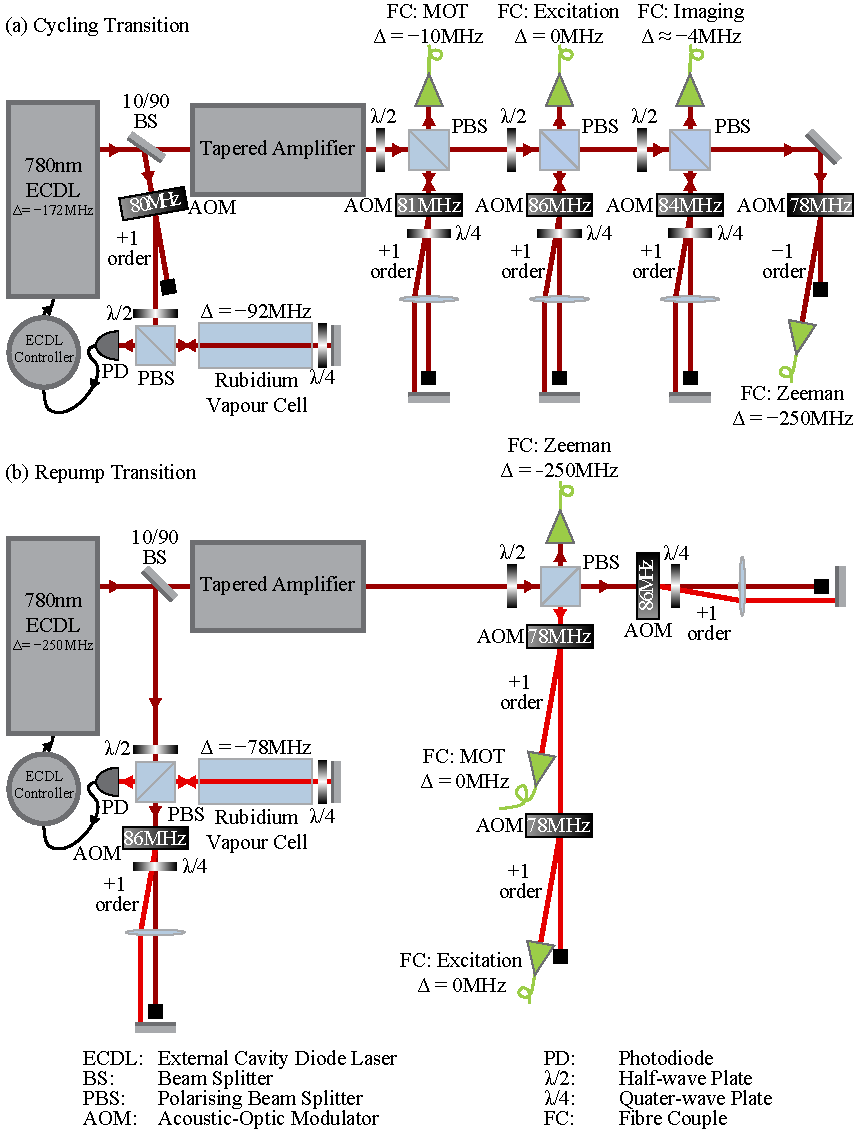
\includegraphics{part2/Figs/laser_setup.pdf}
    \caption[Simplified schematic of the laser setup for the \gls{caeis}.]{The simplified setup of the lasers locked to the rubidium-85 cycling (a) and repump (b) transitions.
    The \glspl{ecdl} are locked with saturated absorption spectroscopy, amplified with tapered amplifiers and frequency-offset using \glspl{aom}.
    $\Delta$s refer to the frequency relative to the cycling or repump transitions.}
    \label{figure:laser_setup}
\end{figure}

\subsection{Rubidium Oven}
The source begins with an effusive rubidium oven with a long heated collimation tube.
Typically effusive ovens are wasteful with large numbers of atoms lost to large solid angles.
This apparatus makes use of a long heated collimation tube to collect and re-emit atoms that were initially emitted at high angles.
These atoms are re-emitted back to the reservoir or into the collimated atom beam leaving the collimation tube.
The rubidium reservoir was typically heated to \unit[80]{$^\circ$C} and the collimation tube to \unit[120]{$^\circ$C}.
Detail on the design, operation, and performance of the oven can be found in References~\cite{bell_slow_2010} and \cite{bell_cold_2011}.

\begin{figure}
    \center
    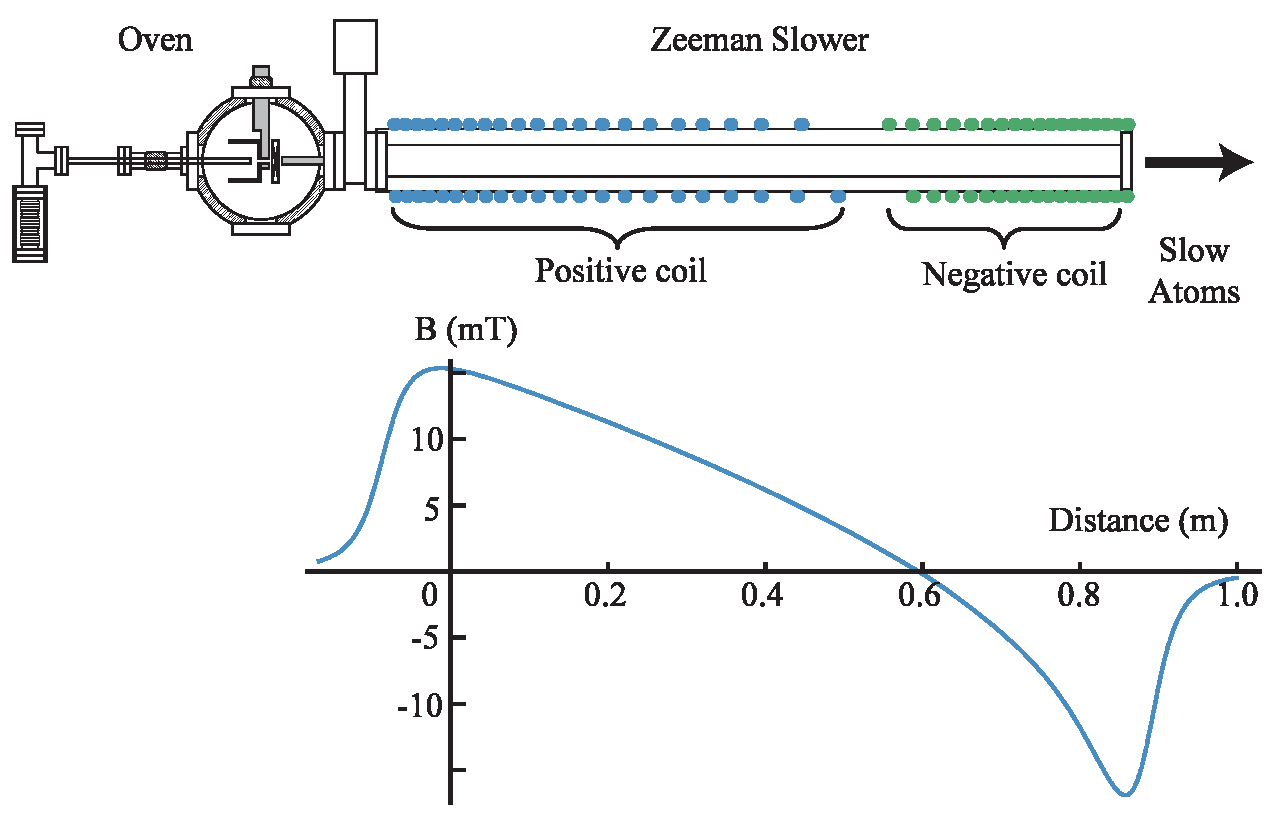
\includegraphics[width=145mm]{part2/Figs/ZeemanOven.pdf}
    \caption[A schematic of the rubidium atom source.]{A schematic of the rubidium atom source. Atomic vapour from the oven is directed into the Zeeman slower where a laser detuned from the atomic resonance (shown in red), in combination with a tapered magnetic coil (blue and green), with a magnetic field as shown, slows the thermal atoms.}
    \label{figure:zeemanoven}
\end{figure}

\subsection{Zeeman Slower}
A Zeeman slower using a solenoid with tapered winding pitch is used to slow the atoms so that they can be captured by the \gls{mot}~\cite{bell_slow_2010}.
Zeeman slowers operate by using a laser red-detuned from resonance to slow the atoms down but as the atoms slow the conditions for resonance change due to the changing Doppler shift thus preventing further slowing of the atoms.
The solution to this quandary used here was a tapered magnetic coil that applied a magnetic field to shift the atomic resonance such that a particular velocity class of atoms remained resonant with the light field, and thus was slowed, along the length of the Zeeman slower.
Atoms leaving the Zeeman slower typically had velocities around \unit[35]{m/s}, well within the capture velocity of the \gls{mot}.
A schematic of the Zeeman slower along with the magnetic field produced by the tapered coil is shown in Figure~\ref{figure:zeemanoven}.

When extracting electrons from the \gls{mot} the magnetic coil must be turned off to prevent disruptions to the electron trajectory.

\subsection{Magneto-Optic Trap}
\glsreset{mot}\Glspl{mot} use a combination of magnetic and light fields to trap and cool atoms to $\muup$K temperatures~\cite{metcalf_laser_1999}.
In the \gls{caeis} the \gls{mot} was formed from six counter propagating \unit[780]{nm} lasers in a retro-reflective quasi-mirror \gls{mot} configuration~\cite{hanssen_using_2006,mcculloch_generation_2013} to allow for the accelerator structure which consisted of transparent and reflective electrodes, as shown in Figure~\ref{figure:mot}.
The magnetic component of the \gls{mot} was formed from two magnetic coils in an anti-Helmholtz configuration providing a zero-field region in the centre of the trap.

The \gls{mot} trapping lasers were detuned \unit[$-10$]{MHz} from the cycling transition and were mixed with on-resonant light at the repump transition to pump atoms that fell into the dark $F=2$ state.

\begin{figure}
    \center
    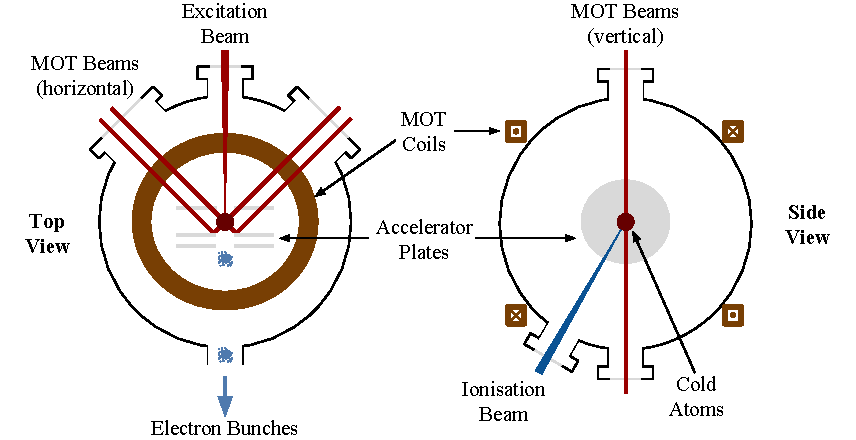
\includegraphics[width=145mm]{part2/Figs/MOTdiagram.pdf}
    \caption[A diagram of the magneto-optic trap.]{A diagram of the magneto-optic trap, ionisation lasers and accelerator structures.}
    \label{figure:mot}
\end{figure}

\subsection{Ionisation}\label{section:two_stage_ionisation}

The \gls{caeis} was capable of generating bunches of electron and ions with long (\unit[$\sim$10]{$\muup$s}), short (\unit[$\sim$5]{ns}), and ultrashort (\unit[$\sim$10]{ps}) bunch duration depending on the laser systems used~\cite{speirs_identification_2017,speirs_electron_2017}.
Depending on the ionisation pathway, the \gls{caeis} was able to produce cold electron bunches (\unit[$\sim$10]{K}) or hotter electron bunches (\unit[$>$10]{K}).
Generally cold electron bunches were preferable and desired bunch duration depended on the application, \gls{ued} for example requires ultrashort bunches.

Rubidium has a ground state ionisation threshold of \unit[4.18]{eV} which can be generated using one blue and one red photon.
Red light could be generated by a \gls{cw} diode laser amplified by a \gls{ta} and locked to the cycling transition or it could be generated with a mode-locked Ti:sapphire amplified pulsed laser with a wavelength range of \unit[770]{nm} to \unit[830]{nm} and a minimum pulse length of \unit[35]{fs}.
Blue light could be generated with a tunable dye pulse laser that produced \unit[460 to 490]{nm} light with a \gls{fwhm} duration of \unit[5]{nm} or with a \gls{cw} laser generated by a high-power tunable frequency-doubled diode laser.

Sequential ionisation utilised a single red photon to excite from the ground state to an intermediate excited state followed by a single blue photon to transition to a field-ionising state or to the ionisation continuum.
For sequential ionisation, the bunch duration was determined by the shortest of the duration of the laser pulse driving the transition from the exited state to the ionising state, the lifetime of the intermediate state, or by the depletion time of the intermediate state.

Multiphoton excitation occurs when the laser intensities are high enough for nonlinear optical transitions to occur which was the case when the red or blue pulse lasers were tightly focused into the atom cloud.
In multiphoton excitation two or more photons are absorbed without transitioning via a real intermediate state.
If $n$ is the number of photons absorbed for the atom to reach its final ionised state then the transition rate is proportional to the $n$th power of the optical intensity~\cite{joachain_atoms_2011}.
Due to the short lifetime of the virtual intermediate states the bunch duration is determined by the duration of the laser pulses.
Multiphoton excitation can occur with just photons of one colour or with photons of both colours.

\Gls{tcmpe} occurs when one blue and one red photon are absorbed but the intermediate state is a virtual state.
Due to the short lifetime of the intermediate state the duration of bunches produced by \gls{tcmpe} depends on duration of the shortest laser pulse.

\Gls{rempe} occurs when there is a combination of sequential excitation and multiphoton excitation.
Here a number of photons are absorbed to excite the atom to a real intermediate state followed by more photons of the same colour being absorbed to transition to the final state.
As less photons are required for each transition the overall transition rate can be much higher when compared to plain multiphoton excitation.

\begin{figure}
    \center
    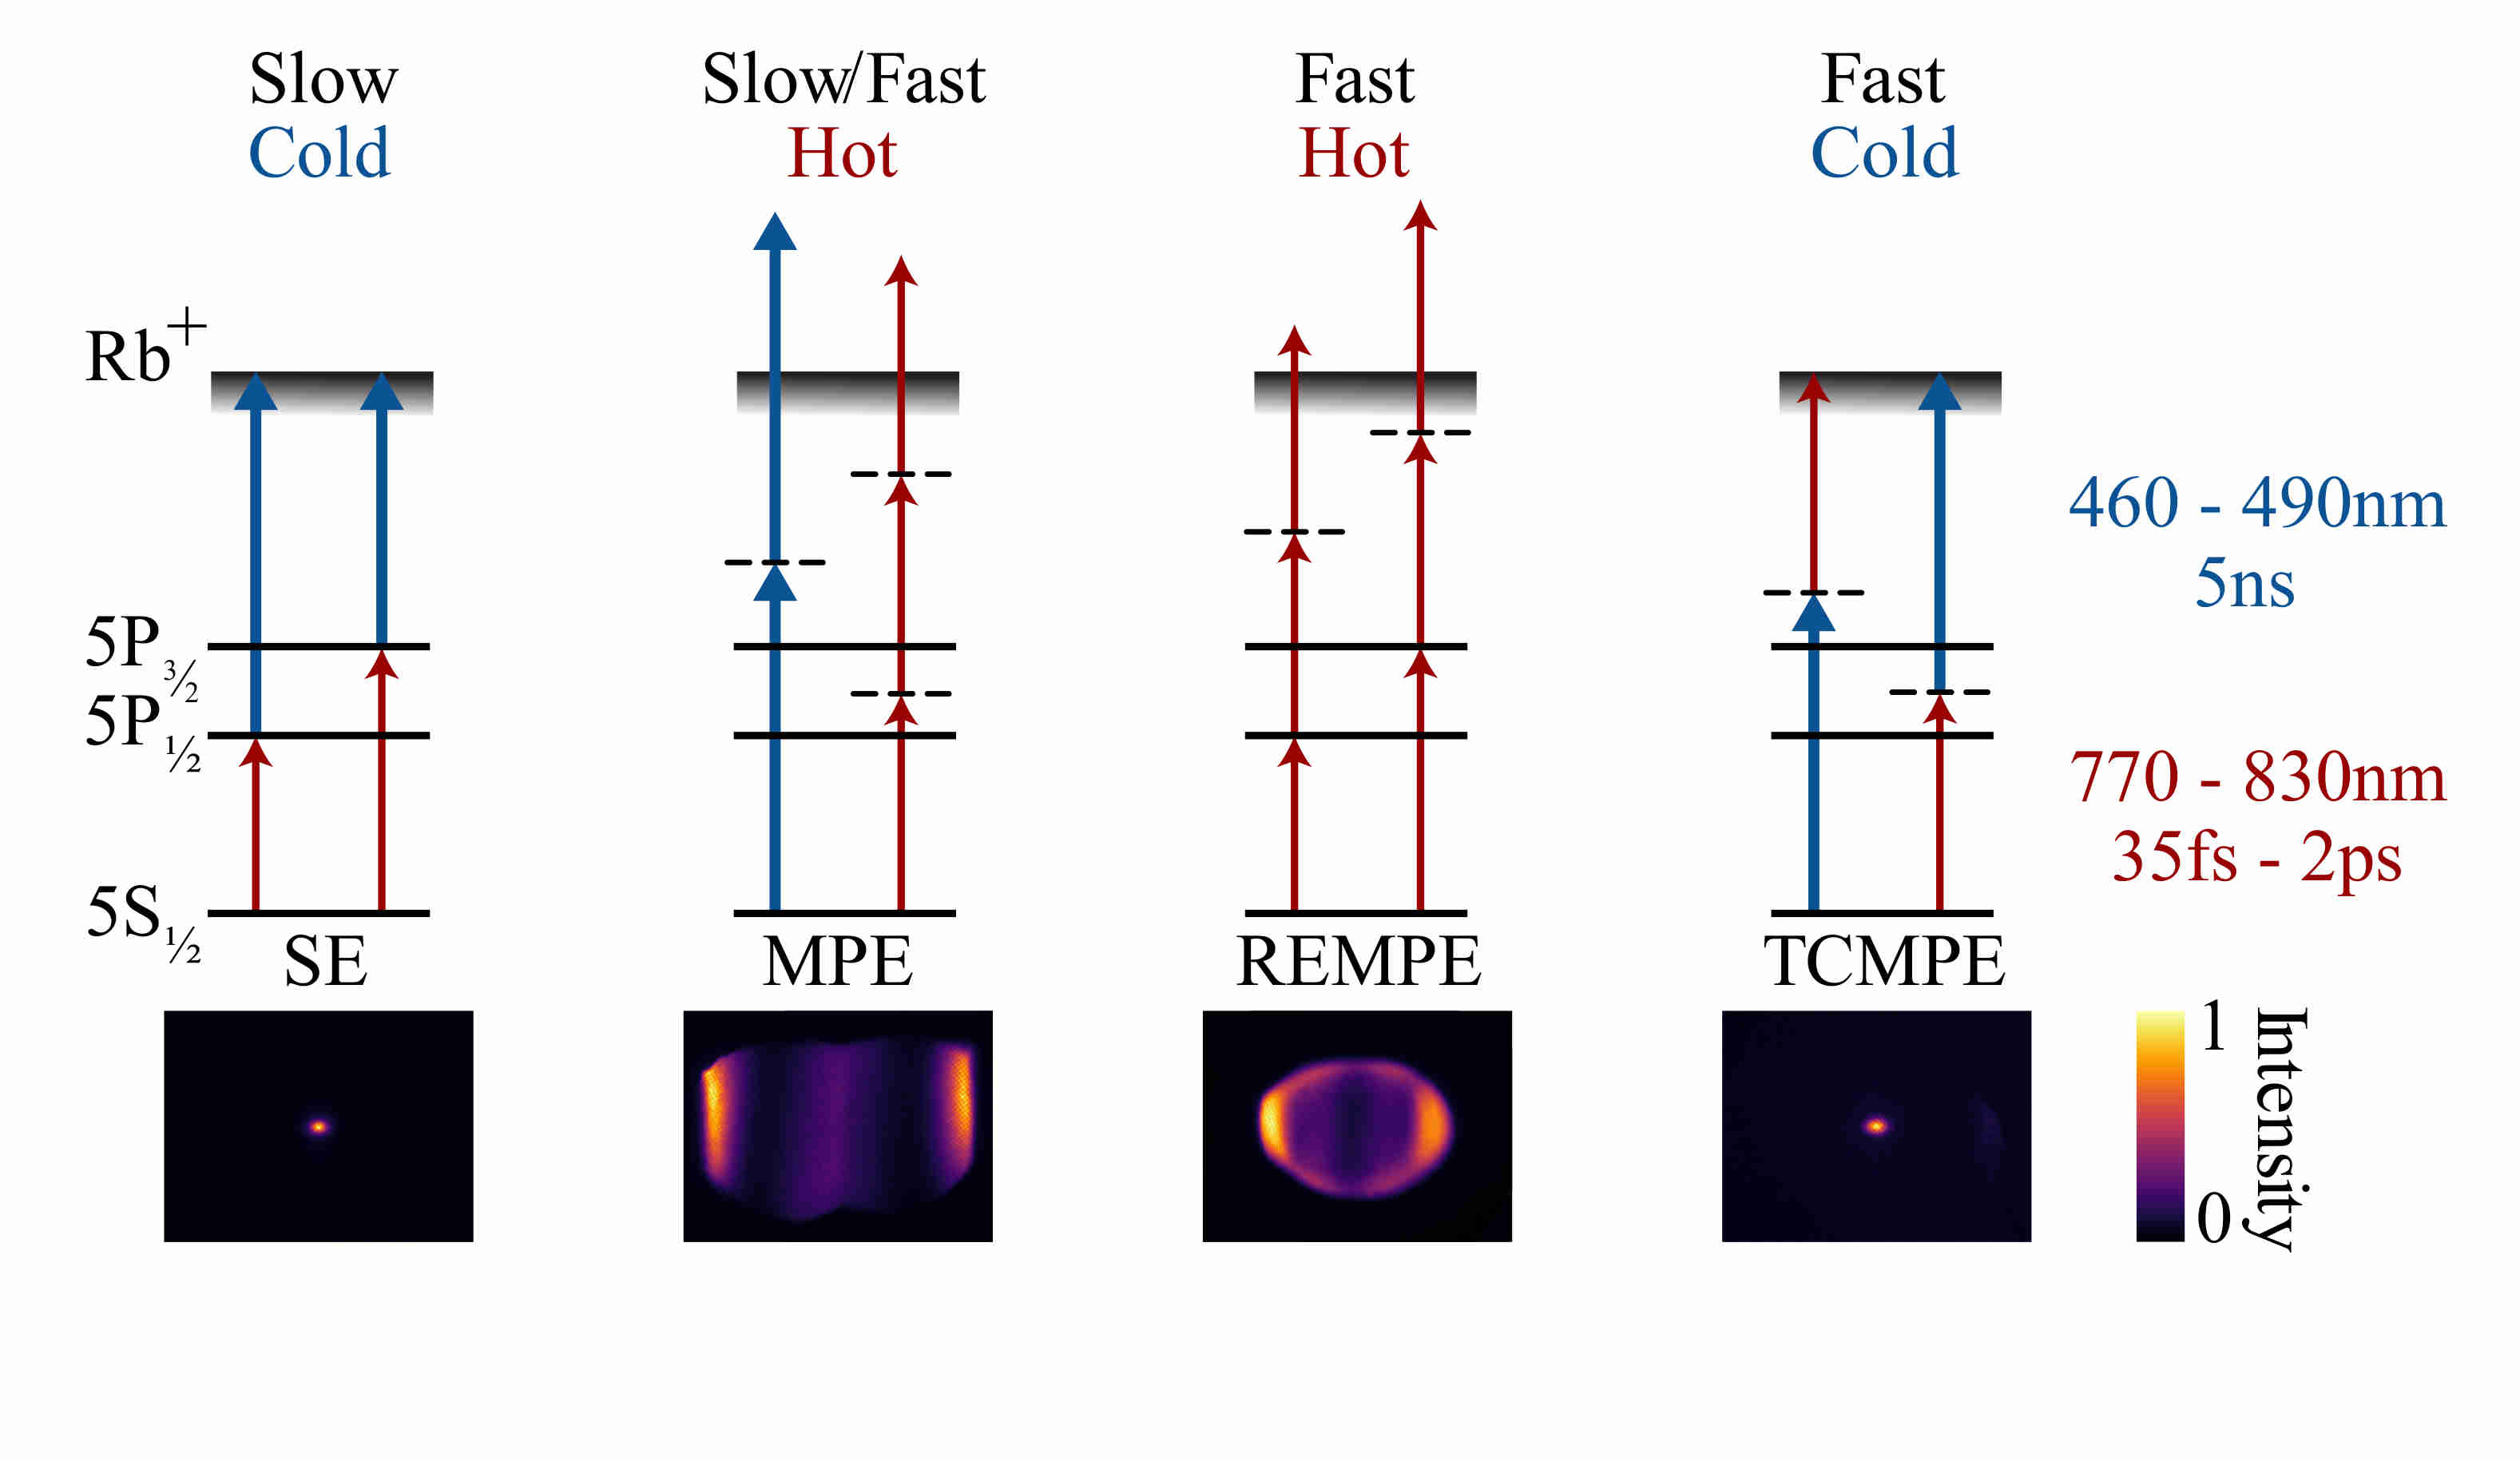
\includegraphics[width=0.75\linewidth]{part2/Figs/ionisationmodes.jpg}
    \caption[Photoexcitation pathways.]{A number of photoexcitation pathways were possible in the presence of high intensity illumination by the red a blue lasers in the \gls{caes} such as sequential excitation (SE), multiphoton excitation (MPE), resonance-enhanced multiphoton excitation (REMPE), and two-colour multiphoton excitation (TCMPE). TCMPE is the only pathway that produces bunches that are cold and ultrashort. The images show the relative transverse momentum distributions for the detected bunches.
    This figure is from Reference~\cite{speirs_electron_2017}.}
    \label{figure:ionisation_modes}
\end{figure}

The temperature of particles generated from the \gls{caes} depends primarily on the excess ionisation energy given to the atoms by the absorbed photons.
Due to the complex spatial probability distributions of electrons in high-lying states the relationship between absorbed photon energy and temperature is complex~\cite{mcculloch_high-coherence_2013} but it is generally true that with greater photon energy comes greater source temperature.
The classical ionisation threshold is lower in the presence of electric field, such as the accelerating field in the \gls{caeis}, due to the Stark-shift.
The excess energy of an ion or electron relative to the classical ionisation threshold is:
\begin{equation}\label{equation:ionisation_energy_stark}
\Delta E = -E_I + 2\sqrt{ke^3F} + \sum_{i=0}^{n}{\frac{hc}{\lambda_i}},
\end{equation}
where $E_I=4.18$\,eV is the ground state ionisation energy of rubidium-85, $k$ is the Coulomb constant, $e$ is the elementary charge, $F$ is the strength of the electric field, $h$ is the Planck constant, and $c$ is the speed of light.
The second term represents the Stark-shift of the classical ionisation threshold, and the last term is the sum of the energy of the $n$ photons involved in the ionisation, with wavelengths $\lambda_i$.
Equation~\ref{equation:ionisation_energy_stark} assumes that rubidium is hydrogen-like which is a good approximation as long as $E_I \gg 2\sqrt{ke^3F}$~\cite{gallagher_rydberg_2005}.

Sequential excitation and \gls{tcmpe} are the only ionisation processes that produced cold electrons as the atoms underwent field ionisation due to the combined photon energy being slightly less than $E_I$.
With the other methods the combined photon energy is larger than $E_I$ and the excess ionisation energy is transferred to the electrons.
The electron bunch temperature was demonstrated experimentally~\cite{speirs_identification_2017} and can be seen in Figure~\ref{figure:ionisation_modes} in the momentum distributions for various ionisation processes.

The duration of the charge particle bunches depended on a number of factors~\cite{speirs_identification_2017}.
Direct ionisation, with combined photon energy greater than $E_I$, resulted in short duration bunches with duration equal to that of the blue laser driving the transition to the ionisation continuum, \unit[5]{ns}.
Excitation to a Rydberg state, followed by field ionisation, resulted in relatively long duration bunches as the bunch duration in this case depends on the lifetime of the Rydberg state, typically 10s of microseconds.
Ionisation by \gls{tcmpe} could result in ultrashort duration bunches, \unit[10]{ps}, if the red femtosecond-duration pulse laser was used to excite the atoms to the virtual intermediate state.

\subsubsection{Beam Shaping}

The \gls{caeis} was able to shape the profile of the electron and ion bunches produced by manipulating the red and blue ionisation laser beams~\cite{mcculloch_arbitrarily_2011}.
The lasers imparted their spatial profiles onto the ionised atoms which, for cold low-emittance bunches, could be maintained to the detector.
The transverse bunch profile was determined by the red excitation laser profile combined with the density profile of the atomic cloud.
Similarly the longitudinal profile depended on the ionisation laser profile and atomic cloud density.

Control over the excitation beam profile was achieved with an \gls{slm} and an iterative feedback system~\cite{van_bijnen_patterned_2015}.
With a second \gls{slm} and control system the longitudinal profile could also be controllable which would allow for full three-dimensional control over the beam shape.
A schematic of the bunch profile system is shown in Figure~\ref{figure:beam_shaping_schematic} and an example of its performance can be seen in Figure~\ref{figure:beam_shaping}.

\begin{figure}
    \center
    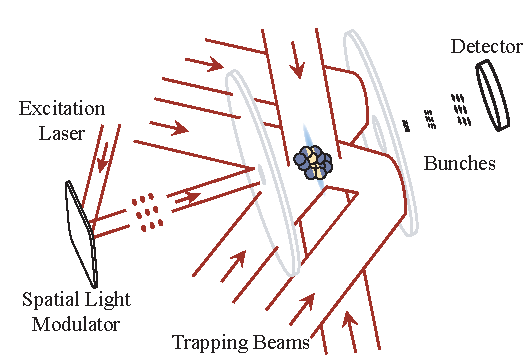
\includegraphics{part2/Figs/beam_shaping_schem.pdf}
    \caption[A schematic of the apparatus used to produce arbitrarily shaped bunches.]{A schematic of the apparatus used to produce arbitrarily shaped bunches. The excitation laser pulse is shaped with an \gls{slm} to form an arbitrary beam profile at the atom cloud, imparting that profile onto the bunch produced by the \gls{caeis}. In this diagram the blue ionisation laser comes from behind the atom cloud.}
    \label{figure:beam_shaping_schematic}
\end{figure}

\begin{figure}
    \center
    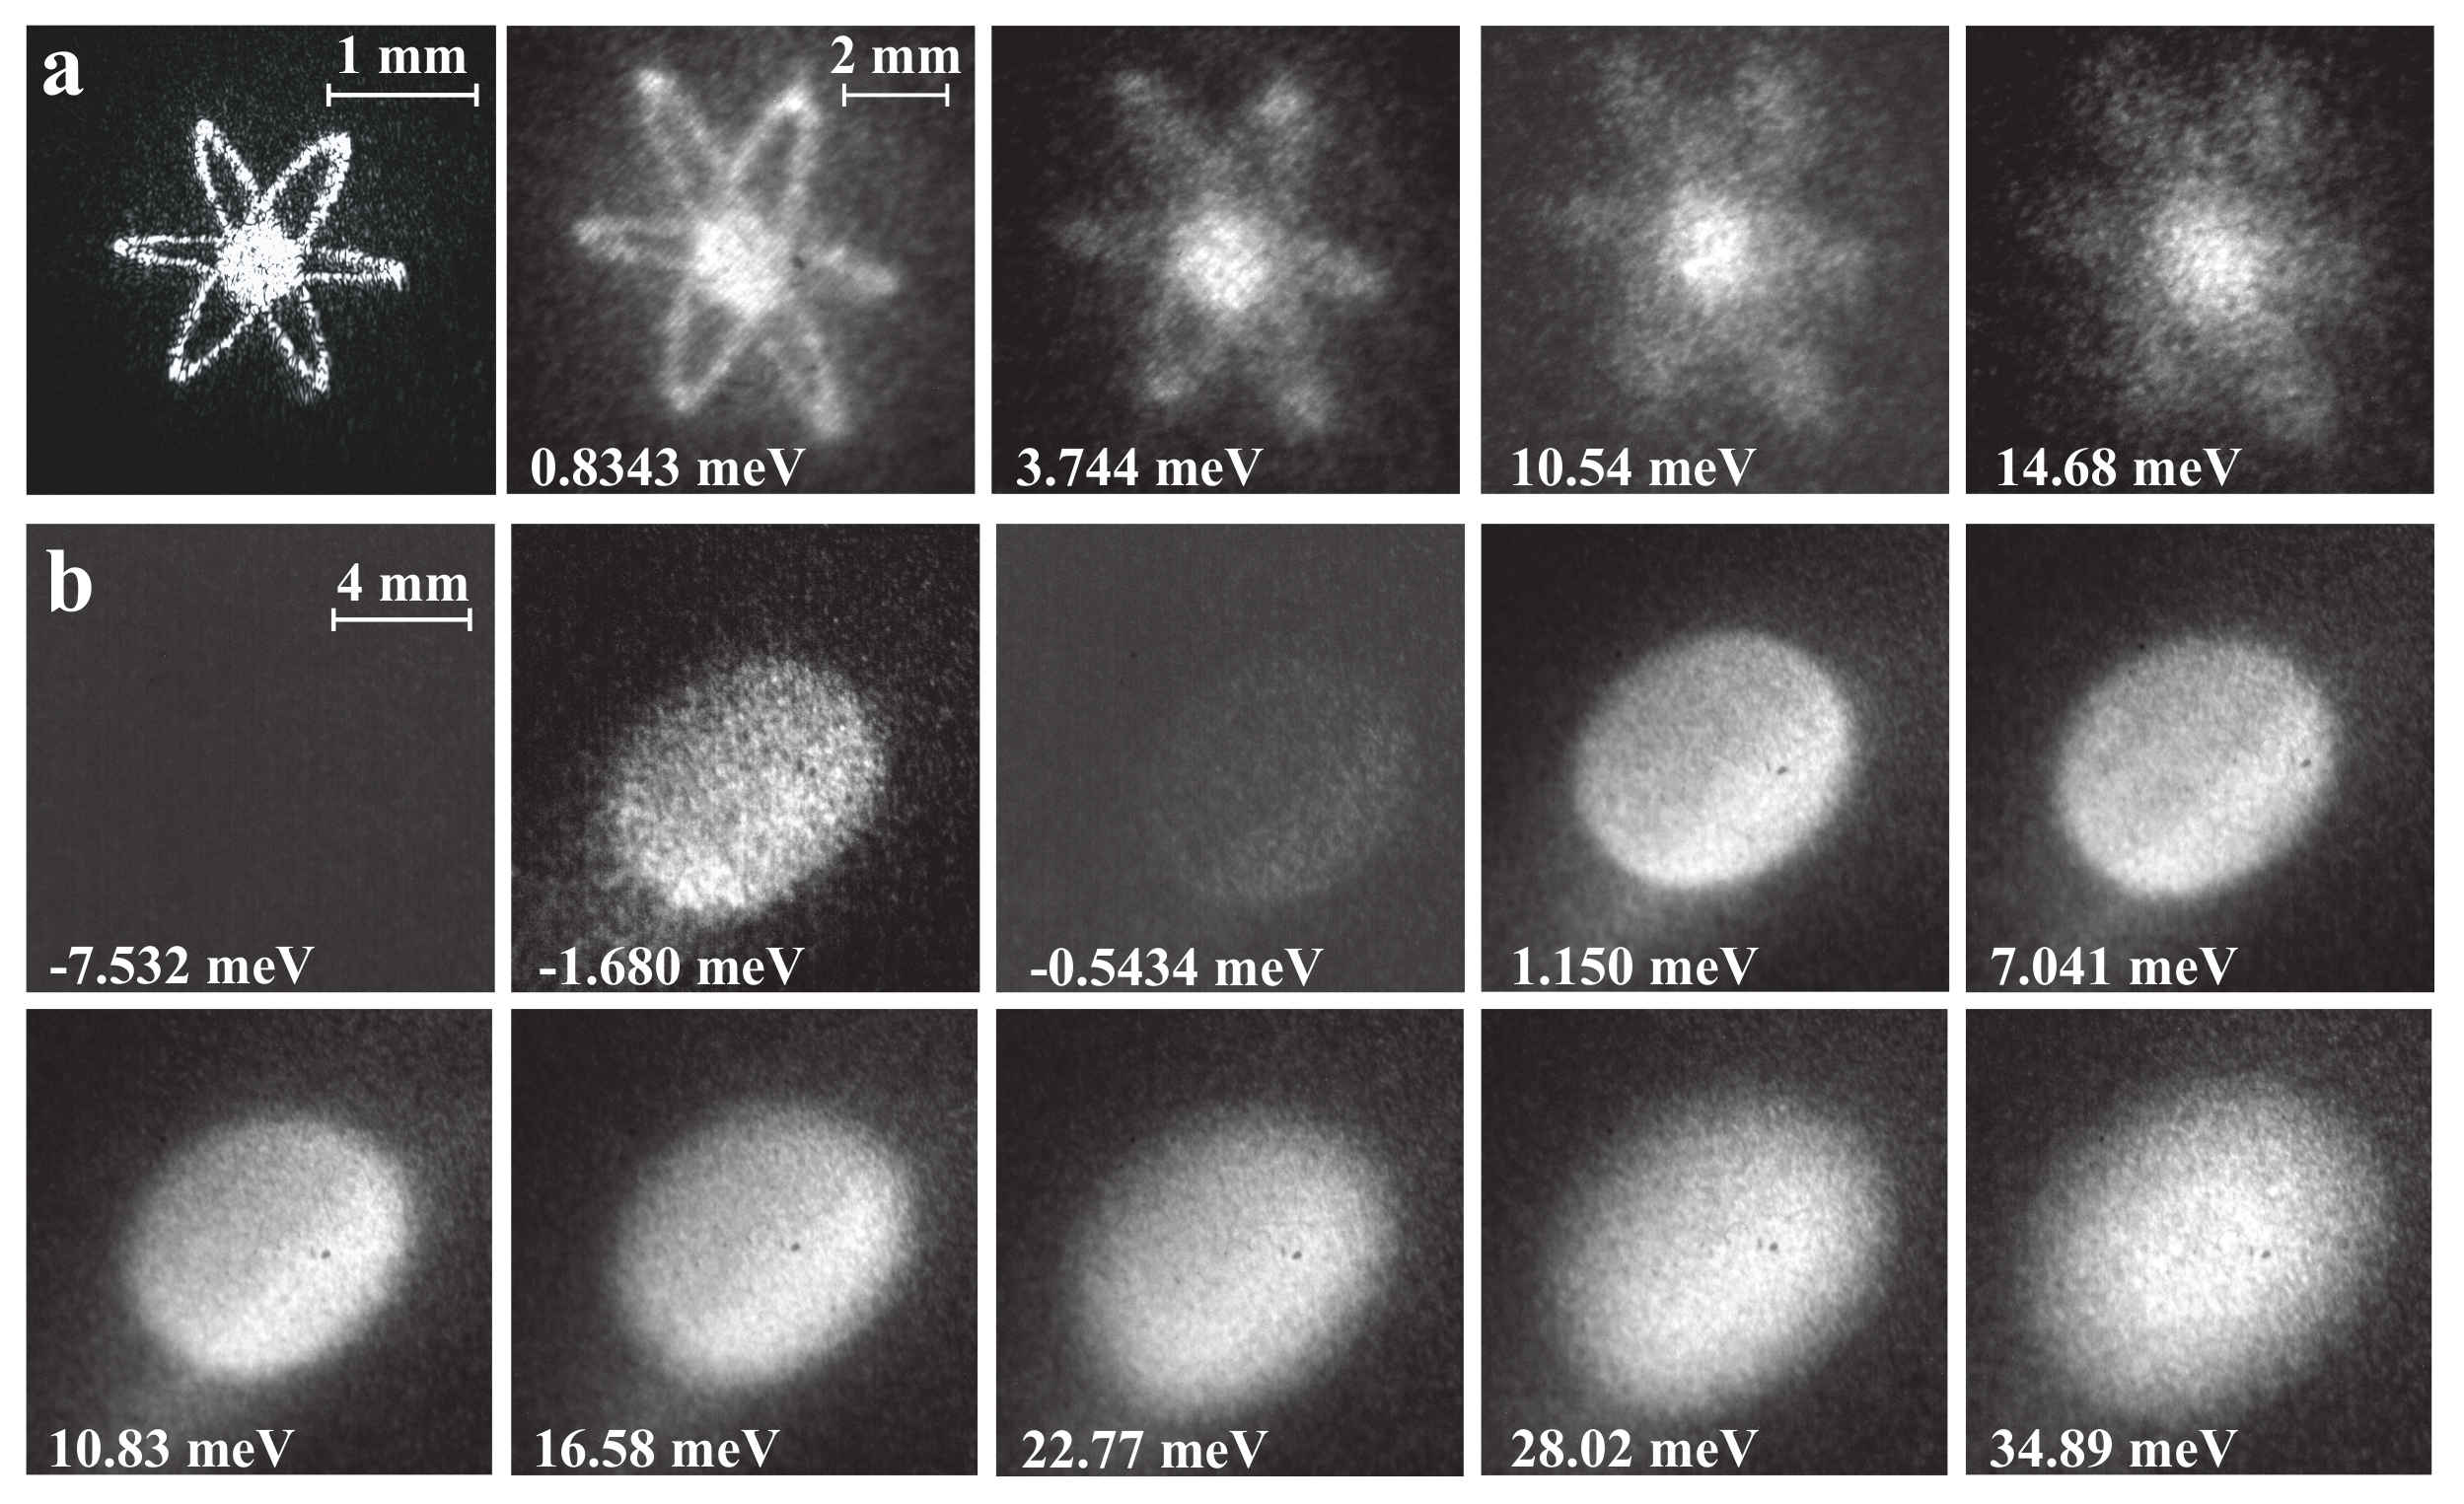
\includegraphics{part2/Figs/beam_shaping.jpg}
    \caption[Beam shaping and the effects of temperature.]{An example of beam shaping and the effects of temperature on the bunch profile.
    \textbf{a}~The left most image indicates the excitation laser profile, and the other images are the transverse electron bunch profiles as excess ionisation energy is varied.
    \textbf{b}~Transverse electron bunch profiles generated by a uniform excitation laser profile as excess ionisation energy is varied.
    The white text indicates the image dimensions and the excess ionisation energy in meV, with negative values being below threshold ionisation.
    At \unit[$-1.680$]{meV} excess ionisation energy the bunch current increases as the ionisation laser couples to a Rydberg state.
    This figure was adapted from Reference~\cite{mcculloch_arbitrarily_2011}.}
    \label{figure:beam_shaping}
\end{figure}

Control over the bunch profile allows for customisation and feedback for whatever application the \gls{caeis} is being used for but is of particular interest for countering space-charge expansion.
Self-interactions between charged particles within a sufficiently dense bunch, referred to as space-charge expansion or Coulomb expansion, results in degradation in the quality of a bunch.
The loss of beam quality is usually expressed as an increase in emittance (see Chapter~\ref{chapter:brightness} for a definition of emittance).
Increases in bunch emittance also results in a decrease in coherence which has ramifications for imaging applications.
With the electron bunch charges achieved to date only the ultrashort duration electron bunches are dense enough to experience significant space-charge expansion.
Ion bunches produced by this source are usually dense enough to demonstrate space-charge.
Suppression of space-charge expansion has been demonstrated with the \gls{caeis} by using beam shaping to produce bunches with linear and reversible Coulomb expansion~\cite{luiten_how_2004,thompson_suppression_2016}.

\subsection{Accelerator}

The static accelerating electric field was generated by two electrodes which were approximately \unit[11]{cm} in diameter and \unit[4]{mm} thick.
One electrode was transmissive and \gls{ar} coated at \unit[780]{nm} and coated with indium-tin-oxide which is also transmissive to \unit[780]{nm} to 96\%.
The second electrode was reflective and composed of polished gold-coated copper.
Each of the electrodes had an aperture in the centre to allow the electron and ion bunches to pass through.

The limit to the beam energy the apparatus was able to produce, approximately \unit[12]{keV}, was determined by the maximum voltages that could be applied to the electrodes; any higher and the electrodes would begin to either arc or short.

\subsection{Beam Optics}

There were a number of systems in place for manipulating the electron and ion beams: a solenoid lens, an Einzel lens, a magnetic quadrupole lens, a one-axis deflector, and a number of permanent magnets located outside the vacuum system.
A schematic of the beamline is shown in Figure~\ref{figure:full_beam_apparatus}.
The lenses were used to focus the bunches, usually to a focus on the detector but sometimes to manipulate the size of the beam at the sample plane.
The quadrupole lens was used to counter astigmatism in the beam and is discussed in more detail in Section~\ref{section:quadrupole}.
The deflector was located after the sample stage and was used to streak bunches across the detector for the results presented in Chapter~\ref{chapter:brightness}.
The permanent magnets were used to steer electron bunches through the system, through a number of apertures and countering the deflection imposed by a number of anomalous magnetic fields present with the \gls{caeis}.

\begin{figure}
    \center
    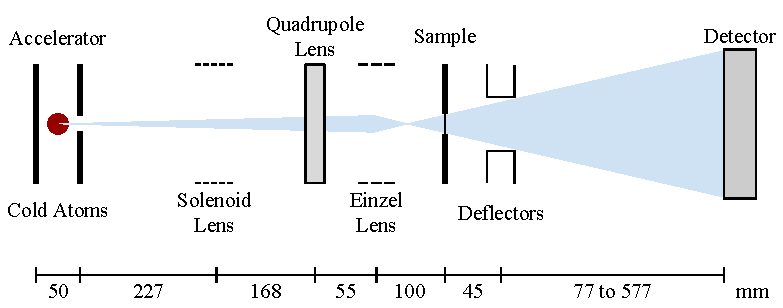
\includegraphics{part2/Figs/FullApparatusSchematic.pdf}
    \caption[Beam optics schematic.]{A schematic of the optics along the charged particle beamline in the \gls{caeis}. The atoms are trapped in a \gls{mot} (not shown) located between two accelerator electrodes. Downstream from the accelerator is a magnetic solenoid lens, a magnetic quadrupole lens, an electrostatic Einzel lens, the sample holder, one-dimensional deflectors, and the \gls{mcp} detector mounted on translating bellows with a $z$ range of \unit[500]{mm}. The numbers at the bottom of the figure indicate the distance between elements and the horizontal axis is not to scale.}
    \label{figure:full_beam_apparatus}
\end{figure}

\subsection{Sample Management}

Experimental samples were mounted on a custom sample mount formed from an aluminium paddle that was large enough to mount eight \gls{tem} samples and block any portion of the beam not passing through the samples.
The samples were held by two commercial \gls{tem} mounts attached to the paddle that were able to fit \unit[3.05]{mm} diameter samples with approximately \unit[2]{mm} diameter of the sample visible to the bunches when the sample lid was in place.
Grazing incidence reflection diffraction samples could also be mounted at the end of the paddle as shown in Figure~\ref{figure:sample_holder}.
The sample paddle was mounted on a stage with manual control over two-axis translation transverse to the beam axis, as well as rotation about the horizontal transverse axis.
The sample paddle could also be connected to a high-voltage supply to allow for the sample to be biased to further manipulate the beam energy as described in Section~\ref{section:sample_bias}.

\begin{figure}
    \centering
    \begin{subfigure}{0.49\linewidth}
    \centering
    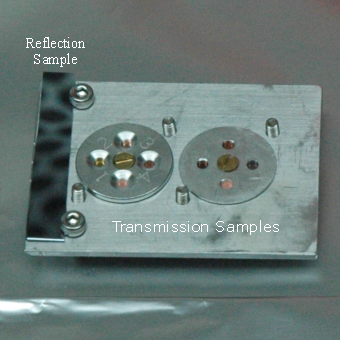
\includegraphics[width=\linewidth]{part2/Figs/sample_holder_alone.pdf}
    \end{subfigure}
    \begin{subfigure}{0.49\linewidth}
    \centering
    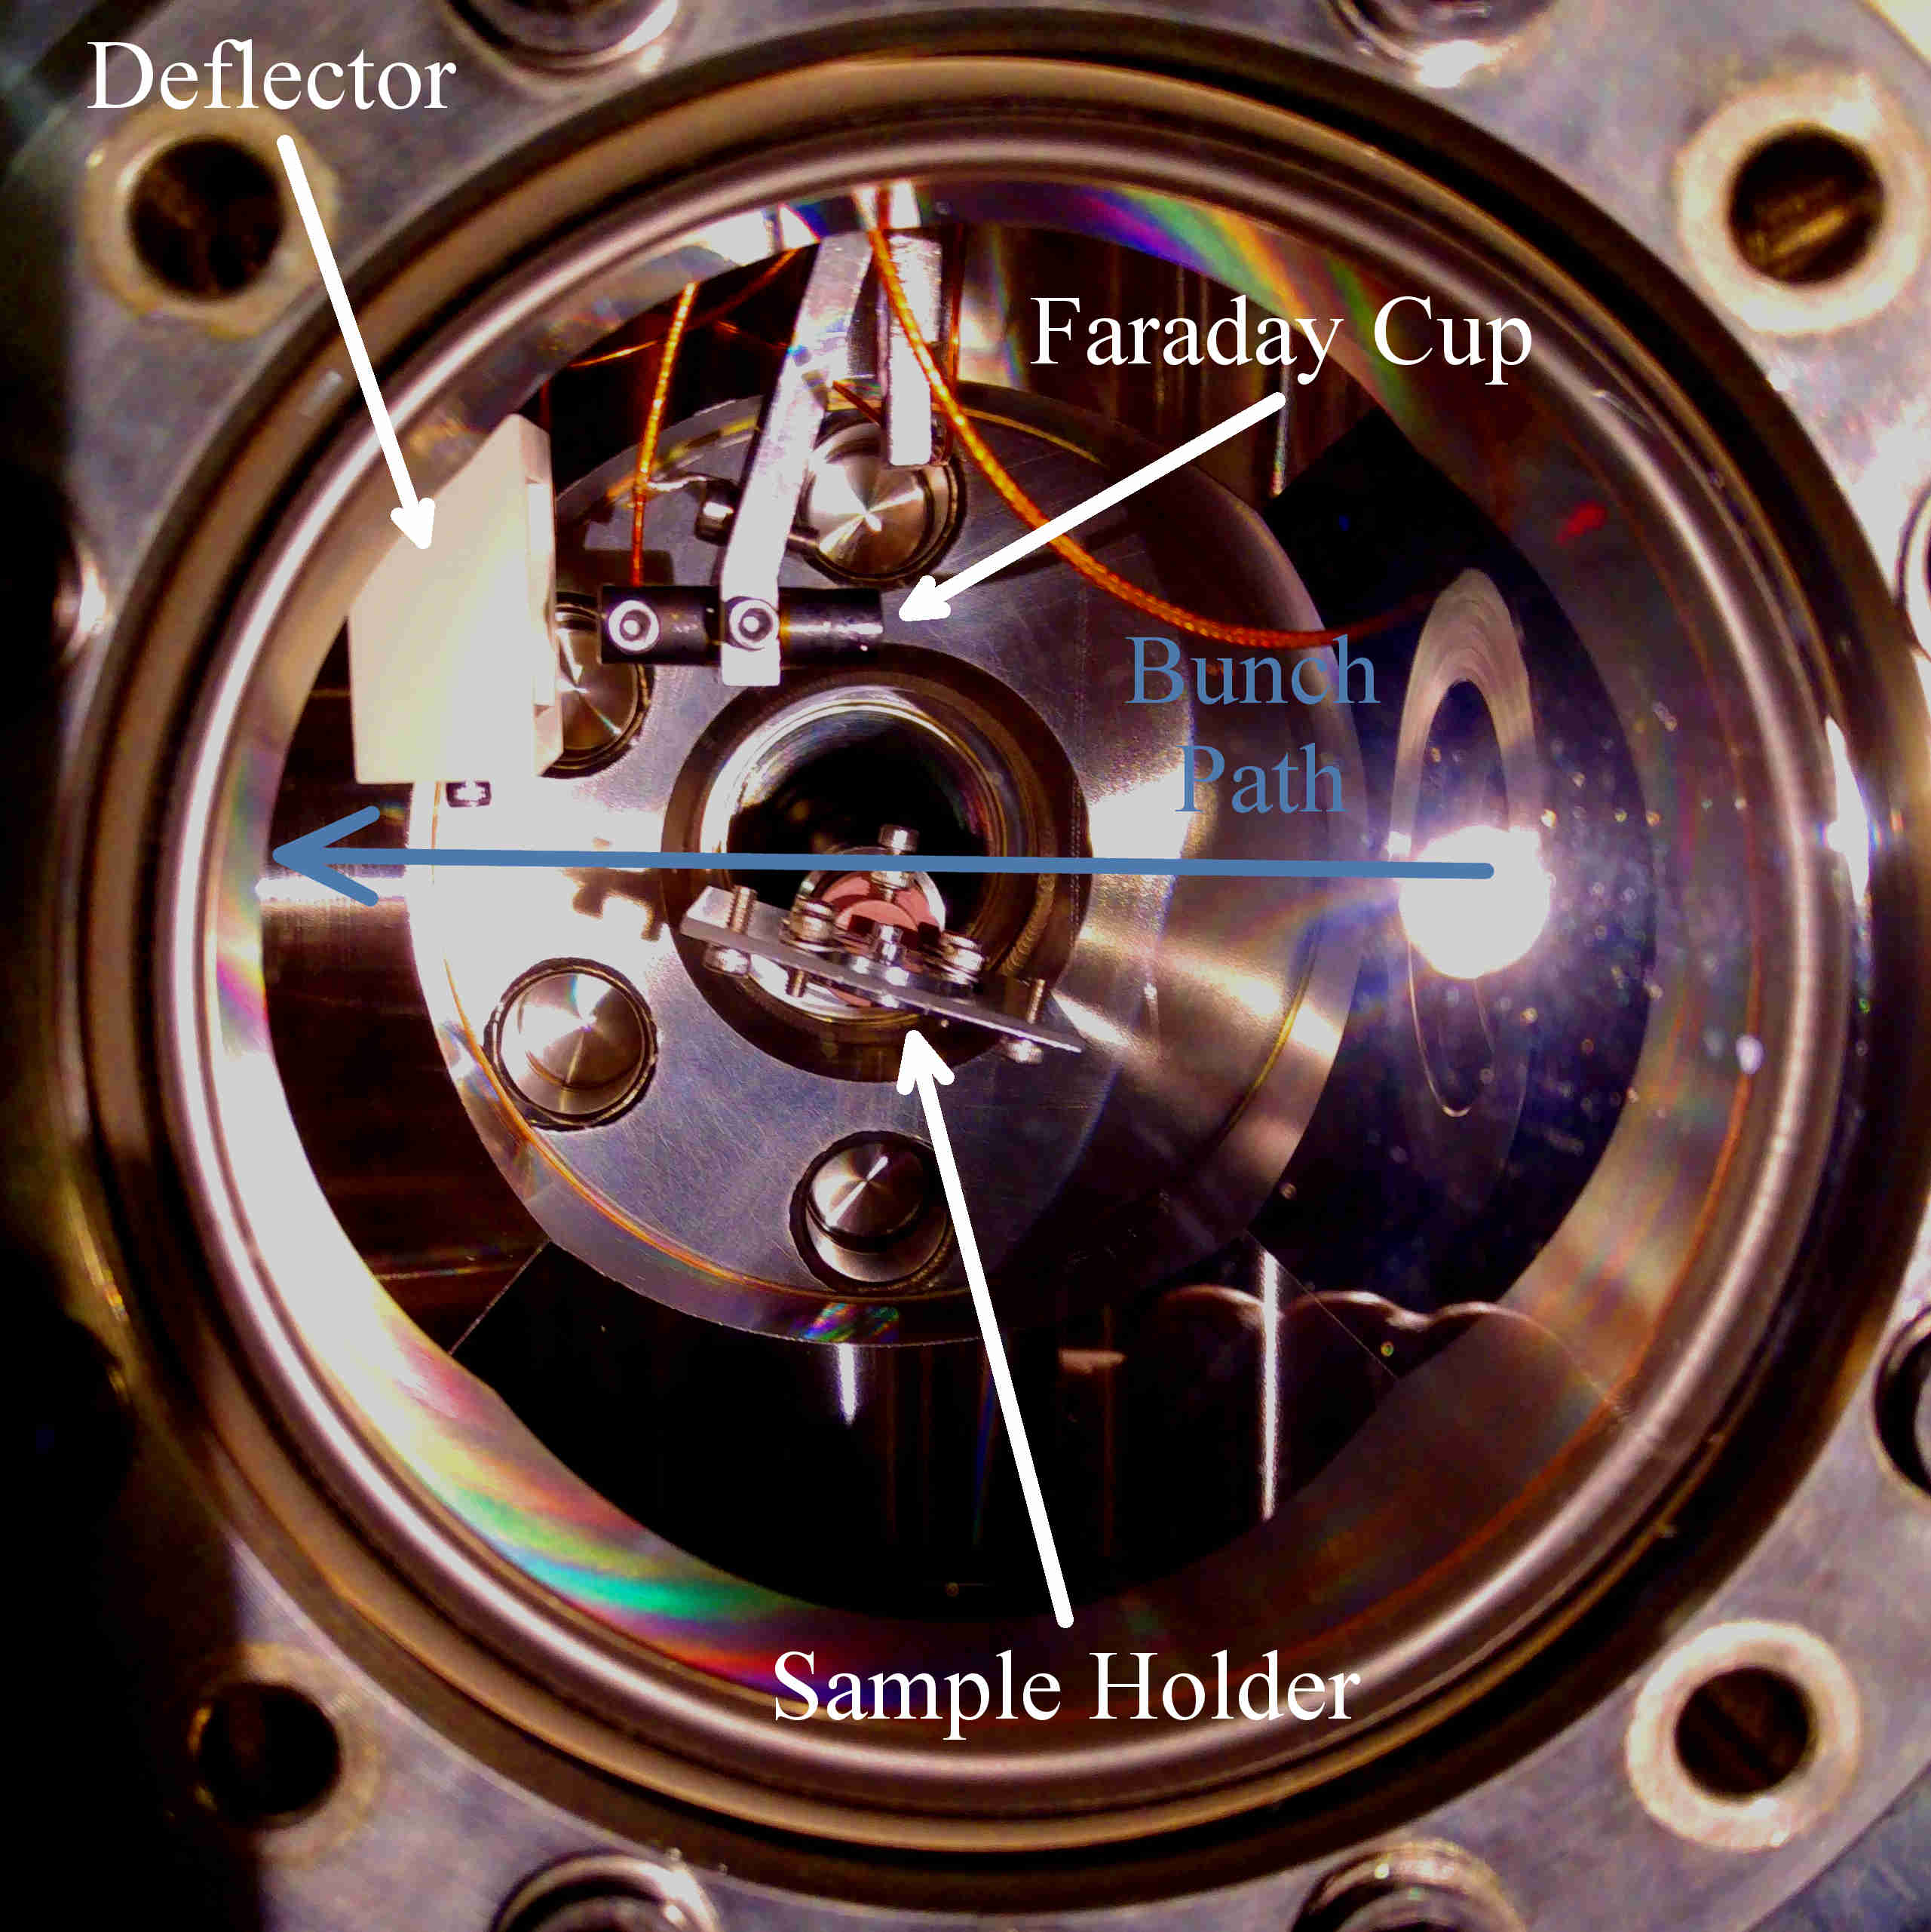
\includegraphics[width=\linewidth]{part2/Figs/sample_holder_in_vitro.jpg}
    \end{subfigure}
    \caption[Sample holder.]{The sample holder used in the \gls{caeis}. In the left photograph the sample holder with eight transmission samples and a reflection sample is shown. On the right is the sample holder in the sample chamber, with the post-sample deflector and Faraday cup retracted from the beam path. Bunches travel from right to left as shown by the blue arrow.}
    \label{figure:sample_holder}
\end{figure}

\subsection{Timing}\label{section:pulse_blaster}

Synchronisation throughout the experiment was achieved with a 24-channel digital timing card\footnote{Spincore Pulseblaster PCI mounted in external USB enclosure.}.
Low voltage TTL signals were used to trigger the numerous time-sensitive devices involved in the experiment.
The \gls{caeis} operated at \unit[10]{Hz}, the frequency of the flashlamp of the \unit[5]{ns} blue pulse laser.
The sequence began with \gls{mot} and Zeeman lasers and fields turning on to load the trap for approximately \unit[90]{ms}.
The trapping lasers and fields were extinguished \unit[5]{ms} before the excitation and ionisation lasers and \gls{ccd} camera were triggered to generate and detect the electron or ion bunch.

\subsection{Current Limitations of the Melbourne CAEIS}

There were a number of factors preventing the \gls{caeis} achieving its goal of electron diffractive imaging that was both single-shot and ultrafast, most importantly the low electron beam current and the instability of the electron trajectory.
These factors also require improvement for other \gls{caeis} goals such as \gls{fib} milling.

The University of Melbourne \gls{caes} was able to generate bunches of $5\times10^5$ electrons when generating \unit[5]{ns} duration bunches, which is of order the charge required for \gls{ued}~\cite{van_oudheusden_compression_2010} but only a few hundred electrons when generating \unit[10]{ps} duration bunches~\cite{speirs_identification_2017}.
There are a few avenues available to the \gls{caeis} to improve the bunch count such as increasing the \gls{mot} density, increasing the power of the ionisation laser, better optimisation of the ionisation pathways~\cite{mcculloch_field_2017}, and potentially running the apparatus in \gls{cw} mode.
\Gls{cw} mode has the potential to increase the number of particles per second however some applications would be difficult or impossible without discrete bunches.
An investigation of the performance of the apparatus in \gls{cw} mode is described in Section~\ref{section:pulse_vs_continuous}.

The stability of the source was also problematic, particularly for electron bunches, as a number of transient effects interfered with the path of the beams on timescales from shot-to-shot to minute-to-minute.
Effects such as eddy currents, due to the switching of the strong magnetic fields, in the steel of the vacuum system and optical tables was one of the primary suspects for the perturbations in the beam path.
Other potential sources are the electronic equipment such as power supplies and switches that were placed as far away from the beam path as practical but were still in the vicinity.
The poor stability of the source made some measurements difficult and others impossible.
Multi-shot measurements were required in a number of cases and, due to the drift of the beam, straight averages of the images from the detector resulted in an unusable blur.
Generating usable images for multi-shot measurements required `registration' of the images, set averages where the features in each individual image was aligned with the other images to prevent blurring.
Measurements without sharp features could not be well registered, as the registration algorithms have trouble precisely aligning the images.
Registration is discussed further in Section~\ref{section:registration}.

\section{Pulsed vs Continuous}\label{section:pulse_vs_continuous}
This \gls{caeis} had not previously been operated as a continuous source and with minor modifications it was adapted to act as a continuous source.
Comparing the performance of the source in its usual pulse mode against the performance as a continuous source had the potential to show pathways for improving the pulsed mode.
Continuous operation, if found advantageous, could have provided an alternative that could be used to demonstrate particular applications, such as \glsreset{cdi}\gls{cdi}, that do not require the source to be pulsed.
Continuous mode functions by using the two-stage ionisation and acceleration on the atom beam from the oven without cooling or trapping by the Zeeman slower and \gls{mot}.
It was hoped that the average beam current would increase with this mode of operation and that the beam produced would be subject to less drift and instability as the large magnetic fields were not switching.
This investigation of continuous operation also, almost serendipitously, permitted a more detailed investigation of the instabilities in the electron trajectory as it provided an opportunity to examine the temporal behaviour of the instability, something not possible when the source operates at a mere \unit[10]{Hz}.

While the entire apparatus and control system had been designed to operate in pulse mode it was fortunately relatively simple to modify the setup to operate to continuously produce an electron beam.
The lasers and magnetic field of the \gls{mot} were disabled, the excitation beam was left on, and the \gls{cw} blue laser was used instead of the usual blue pulse laser to drive ionisation.

Before switching to continuous mode the \gls{caeis} had been measured to have \unit[$0.42\times10^6$]{electrons per bunch} equating to a beam current of \unit[$4.2\times10^6$]{electrons per second}.
Initially the continuous mode was producing \unit[$0.64\times10^6$]{electrons per second} however there were a number of optimisations available to improve the current, as detailed below.

\subsection{Oven Temperature to Electron Count}
When operating in pulsed mode the \gls{mot} was given more than enough time to saturate and thus there was no benefit to producing more atoms from the oven.
In continuous mode the beam current was dependent on the density of atoms in the ionisation region which could be increased by increasing the atomic flux from the rubidium oven.

The atomic flux from the oven could be increased by running the oven at a higher temperature.
During normal operation the oven was set to a temperature of approximately \unit[80]{$^\circ$C} (rubidium has a melting point of \unit[39.30]{$^\circ$C}) however the oven was able to operate at up to \unit[200]{$^\circ$C}.
Previous measurements indicate that the atomic flux from the oven was \unit[$5\times10^9$]{cm$^{-2}$s$^{-1}$} at \unit[80]{$^\circ$C} and increased approximately linearly to \unit[$2\times10^{10}$]{cm$^{-2}$s$^{-1}$} at \unit[200]{$^\circ$C}~\cite{bell_slow_2010}.

The effects of the oven temperature on the beam current are shown in Figure~\ref{figure:oven_counts}.
There was a significant increase in the electron beam current as the oven temperature was increased.
With the oven at a high temperature the beam current was greater than that of the pulsed mode bunches.
An unfortunate side effect of running the oven at high temperatures is that the lifetime of the \unit[5]{g} rubidium ampule in the oven will be reduced.
Given the atomic flux measurements in Reference~\cite{bell_slow_2010}, running the rubidium oven at \unit[200]{$^\circ$C} will reduce the ampule lifetime by approximately a factor of four.
This data indicates that the \gls{cw} beam current could be improved with the use of transverse compression of the atom beam which would provide a similar improvement to beam current as more atoms would be present in the ionisation region~\cite{tielen_development_2015}.

\begin{figure}
    \center
    %% Creator: Matplotlib, PGF backend
%%
%% To include the figure in your LaTeX document, write
%%   \input{<filename>.pgf}
%%
%% Make sure the required packages are loaded in your preamble
%%   \usepackage{pgf}
%%
%% Figures using additional raster images can only be included by \input if
%% they are in the same directory as the main LaTeX file. For loading figures
%% from other directories you can use the `import` package
%%   \usepackage{import}
%% and then include the figures with
%%   \import{<path to file>}{<filename>.pgf}
%%
%% Matplotlib used the following preamble
%%
\begingroup%
\makeatletter%
\begin{pgfpicture}%
\pgfpathrectangle{\pgfpointorigin}{\pgfqpoint{4.282500in}{2.141250in}}%
\pgfusepath{use as bounding box, clip}%
\begin{pgfscope}%
\pgfsetbuttcap%
\pgfsetmiterjoin%
\definecolor{currentfill}{rgb}{1.000000,1.000000,1.000000}%
\pgfsetfillcolor{currentfill}%
\pgfsetlinewidth{0.000000pt}%
\definecolor{currentstroke}{rgb}{1.000000,1.000000,1.000000}%
\pgfsetstrokecolor{currentstroke}%
\pgfsetdash{}{0pt}%
\pgfpathmoveto{\pgfqpoint{0.000000in}{0.000000in}}%
\pgfpathlineto{\pgfqpoint{4.282500in}{0.000000in}}%
\pgfpathlineto{\pgfqpoint{4.282500in}{2.141250in}}%
\pgfpathlineto{\pgfqpoint{0.000000in}{2.141250in}}%
\pgfpathclose%
\pgfusepath{fill}%
\end{pgfscope}%
\begin{pgfscope}%
\pgfsetbuttcap%
\pgfsetmiterjoin%
\definecolor{currentfill}{rgb}{1.000000,1.000000,1.000000}%
\pgfsetfillcolor{currentfill}%
\pgfsetlinewidth{0.000000pt}%
\definecolor{currentstroke}{rgb}{0.000000,0.000000,0.000000}%
\pgfsetstrokecolor{currentstroke}%
\pgfsetstrokeopacity{0.000000}%
\pgfsetdash{}{0pt}%
\pgfpathmoveto{\pgfqpoint{0.691823in}{0.532919in}}%
\pgfpathlineto{\pgfqpoint{4.028722in}{0.532919in}}%
\pgfpathlineto{\pgfqpoint{4.028722in}{1.926770in}}%
\pgfpathlineto{\pgfqpoint{0.691823in}{1.926770in}}%
\pgfpathclose%
\pgfusepath{fill}%
\end{pgfscope}%
\begin{pgfscope}%
\pgfpathrectangle{\pgfqpoint{0.691823in}{0.532919in}}{\pgfqpoint{3.336899in}{1.393852in}} %
\pgfusepath{clip}%
\pgfsetrectcap%
\pgfsetroundjoin%
\pgfsetlinewidth{1.003750pt}%
\definecolor{currentstroke}{rgb}{0.309804,0.478431,0.682353}%
\pgfsetstrokecolor{currentstroke}%
\pgfsetdash{}{0pt}%
\pgfpathmoveto{\pgfqpoint{1.029684in}{0.596936in}}%
\pgfpathlineto{\pgfqpoint{1.584443in}{0.629190in}}%
\pgfpathlineto{\pgfqpoint{2.270593in}{0.845827in}}%
\pgfpathlineto{\pgfqpoint{2.650166in}{1.273641in}}%
\pgfpathlineto{\pgfqpoint{2.825353in}{1.276714in}}%
\pgfpathlineto{\pgfqpoint{3.238294in}{1.418479in}}%
\pgfpathlineto{\pgfqpoint{3.667920in}{1.479532in}}%
\pgfpathlineto{\pgfqpoint{3.903588in}{1.780648in}}%
\pgfusepath{stroke}%
\end{pgfscope}%
\begin{pgfscope}%
\pgfpathrectangle{\pgfqpoint{0.691823in}{0.532919in}}{\pgfqpoint{3.336899in}{1.393852in}} %
\pgfusepath{clip}%
\pgfsetbuttcap%
\pgfsetroundjoin%
\pgfsetlinewidth{1.003750pt}%
\definecolor{currentstroke}{rgb}{0.000000,0.000000,0.000000}%
\pgfsetstrokecolor{currentstroke}%
\pgfsetdash{{6.000000pt}{6.000000pt}}{0.000000pt}%
\pgfpathmoveto{\pgfqpoint{0.691823in}{0.951074in}}%
\pgfpathlineto{\pgfqpoint{4.028722in}{0.951074in}}%
\pgfusepath{stroke}%
\end{pgfscope}%
\begin{pgfscope}%
\pgfsetrectcap%
\pgfsetmiterjoin%
\pgfsetlinewidth{1.003750pt}%
\definecolor{currentstroke}{rgb}{0.000000,0.000000,0.000000}%
\pgfsetstrokecolor{currentstroke}%
\pgfsetdash{}{0pt}%
\pgfpathmoveto{\pgfqpoint{4.028722in}{0.532919in}}%
\pgfpathlineto{\pgfqpoint{4.028722in}{1.926770in}}%
\pgfusepath{stroke}%
\end{pgfscope}%
\begin{pgfscope}%
\pgfsetrectcap%
\pgfsetmiterjoin%
\pgfsetlinewidth{1.003750pt}%
\definecolor{currentstroke}{rgb}{0.000000,0.000000,0.000000}%
\pgfsetstrokecolor{currentstroke}%
\pgfsetdash{}{0pt}%
\pgfpathmoveto{\pgfqpoint{0.691823in}{0.532919in}}%
\pgfpathlineto{\pgfqpoint{0.691823in}{1.926770in}}%
\pgfusepath{stroke}%
\end{pgfscope}%
\begin{pgfscope}%
\pgfsetrectcap%
\pgfsetmiterjoin%
\pgfsetlinewidth{1.003750pt}%
\definecolor{currentstroke}{rgb}{0.000000,0.000000,0.000000}%
\pgfsetstrokecolor{currentstroke}%
\pgfsetdash{}{0pt}%
\pgfpathmoveto{\pgfqpoint{0.691823in}{1.926770in}}%
\pgfpathlineto{\pgfqpoint{4.028722in}{1.926770in}}%
\pgfusepath{stroke}%
\end{pgfscope}%
\begin{pgfscope}%
\pgfsetrectcap%
\pgfsetmiterjoin%
\pgfsetlinewidth{1.003750pt}%
\definecolor{currentstroke}{rgb}{0.000000,0.000000,0.000000}%
\pgfsetstrokecolor{currentstroke}%
\pgfsetdash{}{0pt}%
\pgfpathmoveto{\pgfqpoint{0.691823in}{0.532919in}}%
\pgfpathlineto{\pgfqpoint{4.028722in}{0.532919in}}%
\pgfusepath{stroke}%
\end{pgfscope}%
\begin{pgfscope}%
\pgfsetbuttcap%
\pgfsetroundjoin%
\definecolor{currentfill}{rgb}{0.000000,0.000000,0.000000}%
\pgfsetfillcolor{currentfill}%
\pgfsetlinewidth{0.501875pt}%
\definecolor{currentstroke}{rgb}{0.000000,0.000000,0.000000}%
\pgfsetstrokecolor{currentstroke}%
\pgfsetdash{}{0pt}%
\pgfsys@defobject{currentmarker}{\pgfqpoint{0.000000in}{0.000000in}}{\pgfqpoint{0.000000in}{0.055556in}}{%
\pgfpathmoveto{\pgfqpoint{0.000000in}{0.000000in}}%
\pgfpathlineto{\pgfqpoint{0.000000in}{0.055556in}}%
\pgfusepath{stroke,fill}%
}%
\begin{pgfscope}%
\pgfsys@transformshift{0.691823in}{0.532919in}%
\pgfsys@useobject{currentmarker}{}%
\end{pgfscope}%
\end{pgfscope}%
\begin{pgfscope}%
\pgfsetbuttcap%
\pgfsetroundjoin%
\definecolor{currentfill}{rgb}{0.000000,0.000000,0.000000}%
\pgfsetfillcolor{currentfill}%
\pgfsetlinewidth{0.501875pt}%
\definecolor{currentstroke}{rgb}{0.000000,0.000000,0.000000}%
\pgfsetstrokecolor{currentstroke}%
\pgfsetdash{}{0pt}%
\pgfsys@defobject{currentmarker}{\pgfqpoint{0.000000in}{-0.055556in}}{\pgfqpoint{0.000000in}{0.000000in}}{%
\pgfpathmoveto{\pgfqpoint{0.000000in}{0.000000in}}%
\pgfpathlineto{\pgfqpoint{0.000000in}{-0.055556in}}%
\pgfusepath{stroke,fill}%
}%
\begin{pgfscope}%
\pgfsys@transformshift{0.691823in}{1.926770in}%
\pgfsys@useobject{currentmarker}{}%
\end{pgfscope}%
\end{pgfscope}%
\begin{pgfscope}%
\pgftext[x=0.691823in,y=0.477363in,,top]{\fontsize{10.000000}{12.000000}\selectfont \(\displaystyle 60\)}%
\end{pgfscope}%
\begin{pgfscope}%
\pgfsetbuttcap%
\pgfsetroundjoin%
\definecolor{currentfill}{rgb}{0.000000,0.000000,0.000000}%
\pgfsetfillcolor{currentfill}%
\pgfsetlinewidth{0.501875pt}%
\definecolor{currentstroke}{rgb}{0.000000,0.000000,0.000000}%
\pgfsetstrokecolor{currentstroke}%
\pgfsetdash{}{0pt}%
\pgfsys@defobject{currentmarker}{\pgfqpoint{0.000000in}{0.000000in}}{\pgfqpoint{0.000000in}{0.055556in}}{%
\pgfpathmoveto{\pgfqpoint{0.000000in}{0.000000in}}%
\pgfpathlineto{\pgfqpoint{0.000000in}{0.055556in}}%
\pgfusepath{stroke,fill}%
}%
\begin{pgfscope}%
\pgfsys@transformshift{1.108935in}{0.532919in}%
\pgfsys@useobject{currentmarker}{}%
\end{pgfscope}%
\end{pgfscope}%
\begin{pgfscope}%
\pgfsetbuttcap%
\pgfsetroundjoin%
\definecolor{currentfill}{rgb}{0.000000,0.000000,0.000000}%
\pgfsetfillcolor{currentfill}%
\pgfsetlinewidth{0.501875pt}%
\definecolor{currentstroke}{rgb}{0.000000,0.000000,0.000000}%
\pgfsetstrokecolor{currentstroke}%
\pgfsetdash{}{0pt}%
\pgfsys@defobject{currentmarker}{\pgfqpoint{0.000000in}{-0.055556in}}{\pgfqpoint{0.000000in}{0.000000in}}{%
\pgfpathmoveto{\pgfqpoint{0.000000in}{0.000000in}}%
\pgfpathlineto{\pgfqpoint{0.000000in}{-0.055556in}}%
\pgfusepath{stroke,fill}%
}%
\begin{pgfscope}%
\pgfsys@transformshift{1.108935in}{1.926770in}%
\pgfsys@useobject{currentmarker}{}%
\end{pgfscope}%
\end{pgfscope}%
\begin{pgfscope}%
\pgftext[x=1.108935in,y=0.477363in,,top]{\fontsize{10.000000}{12.000000}\selectfont \(\displaystyle 80\)}%
\end{pgfscope}%
\begin{pgfscope}%
\pgfsetbuttcap%
\pgfsetroundjoin%
\definecolor{currentfill}{rgb}{0.000000,0.000000,0.000000}%
\pgfsetfillcolor{currentfill}%
\pgfsetlinewidth{0.501875pt}%
\definecolor{currentstroke}{rgb}{0.000000,0.000000,0.000000}%
\pgfsetstrokecolor{currentstroke}%
\pgfsetdash{}{0pt}%
\pgfsys@defobject{currentmarker}{\pgfqpoint{0.000000in}{0.000000in}}{\pgfqpoint{0.000000in}{0.055556in}}{%
\pgfpathmoveto{\pgfqpoint{0.000000in}{0.000000in}}%
\pgfpathlineto{\pgfqpoint{0.000000in}{0.055556in}}%
\pgfusepath{stroke,fill}%
}%
\begin{pgfscope}%
\pgfsys@transformshift{1.526048in}{0.532919in}%
\pgfsys@useobject{currentmarker}{}%
\end{pgfscope}%
\end{pgfscope}%
\begin{pgfscope}%
\pgfsetbuttcap%
\pgfsetroundjoin%
\definecolor{currentfill}{rgb}{0.000000,0.000000,0.000000}%
\pgfsetfillcolor{currentfill}%
\pgfsetlinewidth{0.501875pt}%
\definecolor{currentstroke}{rgb}{0.000000,0.000000,0.000000}%
\pgfsetstrokecolor{currentstroke}%
\pgfsetdash{}{0pt}%
\pgfsys@defobject{currentmarker}{\pgfqpoint{0.000000in}{-0.055556in}}{\pgfqpoint{0.000000in}{0.000000in}}{%
\pgfpathmoveto{\pgfqpoint{0.000000in}{0.000000in}}%
\pgfpathlineto{\pgfqpoint{0.000000in}{-0.055556in}}%
\pgfusepath{stroke,fill}%
}%
\begin{pgfscope}%
\pgfsys@transformshift{1.526048in}{1.926770in}%
\pgfsys@useobject{currentmarker}{}%
\end{pgfscope}%
\end{pgfscope}%
\begin{pgfscope}%
\pgftext[x=1.526048in,y=0.477363in,,top]{\fontsize{10.000000}{12.000000}\selectfont \(\displaystyle 100\)}%
\end{pgfscope}%
\begin{pgfscope}%
\pgfsetbuttcap%
\pgfsetroundjoin%
\definecolor{currentfill}{rgb}{0.000000,0.000000,0.000000}%
\pgfsetfillcolor{currentfill}%
\pgfsetlinewidth{0.501875pt}%
\definecolor{currentstroke}{rgb}{0.000000,0.000000,0.000000}%
\pgfsetstrokecolor{currentstroke}%
\pgfsetdash{}{0pt}%
\pgfsys@defobject{currentmarker}{\pgfqpoint{0.000000in}{0.000000in}}{\pgfqpoint{0.000000in}{0.055556in}}{%
\pgfpathmoveto{\pgfqpoint{0.000000in}{0.000000in}}%
\pgfpathlineto{\pgfqpoint{0.000000in}{0.055556in}}%
\pgfusepath{stroke,fill}%
}%
\begin{pgfscope}%
\pgfsys@transformshift{1.943160in}{0.532919in}%
\pgfsys@useobject{currentmarker}{}%
\end{pgfscope}%
\end{pgfscope}%
\begin{pgfscope}%
\pgfsetbuttcap%
\pgfsetroundjoin%
\definecolor{currentfill}{rgb}{0.000000,0.000000,0.000000}%
\pgfsetfillcolor{currentfill}%
\pgfsetlinewidth{0.501875pt}%
\definecolor{currentstroke}{rgb}{0.000000,0.000000,0.000000}%
\pgfsetstrokecolor{currentstroke}%
\pgfsetdash{}{0pt}%
\pgfsys@defobject{currentmarker}{\pgfqpoint{0.000000in}{-0.055556in}}{\pgfqpoint{0.000000in}{0.000000in}}{%
\pgfpathmoveto{\pgfqpoint{0.000000in}{0.000000in}}%
\pgfpathlineto{\pgfqpoint{0.000000in}{-0.055556in}}%
\pgfusepath{stroke,fill}%
}%
\begin{pgfscope}%
\pgfsys@transformshift{1.943160in}{1.926770in}%
\pgfsys@useobject{currentmarker}{}%
\end{pgfscope}%
\end{pgfscope}%
\begin{pgfscope}%
\pgftext[x=1.943160in,y=0.477363in,,top]{\fontsize{10.000000}{12.000000}\selectfont \(\displaystyle 120\)}%
\end{pgfscope}%
\begin{pgfscope}%
\pgfsetbuttcap%
\pgfsetroundjoin%
\definecolor{currentfill}{rgb}{0.000000,0.000000,0.000000}%
\pgfsetfillcolor{currentfill}%
\pgfsetlinewidth{0.501875pt}%
\definecolor{currentstroke}{rgb}{0.000000,0.000000,0.000000}%
\pgfsetstrokecolor{currentstroke}%
\pgfsetdash{}{0pt}%
\pgfsys@defobject{currentmarker}{\pgfqpoint{0.000000in}{0.000000in}}{\pgfqpoint{0.000000in}{0.055556in}}{%
\pgfpathmoveto{\pgfqpoint{0.000000in}{0.000000in}}%
\pgfpathlineto{\pgfqpoint{0.000000in}{0.055556in}}%
\pgfusepath{stroke,fill}%
}%
\begin{pgfscope}%
\pgfsys@transformshift{2.360273in}{0.532919in}%
\pgfsys@useobject{currentmarker}{}%
\end{pgfscope}%
\end{pgfscope}%
\begin{pgfscope}%
\pgfsetbuttcap%
\pgfsetroundjoin%
\definecolor{currentfill}{rgb}{0.000000,0.000000,0.000000}%
\pgfsetfillcolor{currentfill}%
\pgfsetlinewidth{0.501875pt}%
\definecolor{currentstroke}{rgb}{0.000000,0.000000,0.000000}%
\pgfsetstrokecolor{currentstroke}%
\pgfsetdash{}{0pt}%
\pgfsys@defobject{currentmarker}{\pgfqpoint{0.000000in}{-0.055556in}}{\pgfqpoint{0.000000in}{0.000000in}}{%
\pgfpathmoveto{\pgfqpoint{0.000000in}{0.000000in}}%
\pgfpathlineto{\pgfqpoint{0.000000in}{-0.055556in}}%
\pgfusepath{stroke,fill}%
}%
\begin{pgfscope}%
\pgfsys@transformshift{2.360273in}{1.926770in}%
\pgfsys@useobject{currentmarker}{}%
\end{pgfscope}%
\end{pgfscope}%
\begin{pgfscope}%
\pgftext[x=2.360273in,y=0.477363in,,top]{\fontsize{10.000000}{12.000000}\selectfont \(\displaystyle 140\)}%
\end{pgfscope}%
\begin{pgfscope}%
\pgfsetbuttcap%
\pgfsetroundjoin%
\definecolor{currentfill}{rgb}{0.000000,0.000000,0.000000}%
\pgfsetfillcolor{currentfill}%
\pgfsetlinewidth{0.501875pt}%
\definecolor{currentstroke}{rgb}{0.000000,0.000000,0.000000}%
\pgfsetstrokecolor{currentstroke}%
\pgfsetdash{}{0pt}%
\pgfsys@defobject{currentmarker}{\pgfqpoint{0.000000in}{0.000000in}}{\pgfqpoint{0.000000in}{0.055556in}}{%
\pgfpathmoveto{\pgfqpoint{0.000000in}{0.000000in}}%
\pgfpathlineto{\pgfqpoint{0.000000in}{0.055556in}}%
\pgfusepath{stroke,fill}%
}%
\begin{pgfscope}%
\pgfsys@transformshift{2.777385in}{0.532919in}%
\pgfsys@useobject{currentmarker}{}%
\end{pgfscope}%
\end{pgfscope}%
\begin{pgfscope}%
\pgfsetbuttcap%
\pgfsetroundjoin%
\definecolor{currentfill}{rgb}{0.000000,0.000000,0.000000}%
\pgfsetfillcolor{currentfill}%
\pgfsetlinewidth{0.501875pt}%
\definecolor{currentstroke}{rgb}{0.000000,0.000000,0.000000}%
\pgfsetstrokecolor{currentstroke}%
\pgfsetdash{}{0pt}%
\pgfsys@defobject{currentmarker}{\pgfqpoint{0.000000in}{-0.055556in}}{\pgfqpoint{0.000000in}{0.000000in}}{%
\pgfpathmoveto{\pgfqpoint{0.000000in}{0.000000in}}%
\pgfpathlineto{\pgfqpoint{0.000000in}{-0.055556in}}%
\pgfusepath{stroke,fill}%
}%
\begin{pgfscope}%
\pgfsys@transformshift{2.777385in}{1.926770in}%
\pgfsys@useobject{currentmarker}{}%
\end{pgfscope}%
\end{pgfscope}%
\begin{pgfscope}%
\pgftext[x=2.777385in,y=0.477363in,,top]{\fontsize{10.000000}{12.000000}\selectfont \(\displaystyle 160\)}%
\end{pgfscope}%
\begin{pgfscope}%
\pgfsetbuttcap%
\pgfsetroundjoin%
\definecolor{currentfill}{rgb}{0.000000,0.000000,0.000000}%
\pgfsetfillcolor{currentfill}%
\pgfsetlinewidth{0.501875pt}%
\definecolor{currentstroke}{rgb}{0.000000,0.000000,0.000000}%
\pgfsetstrokecolor{currentstroke}%
\pgfsetdash{}{0pt}%
\pgfsys@defobject{currentmarker}{\pgfqpoint{0.000000in}{0.000000in}}{\pgfqpoint{0.000000in}{0.055556in}}{%
\pgfpathmoveto{\pgfqpoint{0.000000in}{0.000000in}}%
\pgfpathlineto{\pgfqpoint{0.000000in}{0.055556in}}%
\pgfusepath{stroke,fill}%
}%
\begin{pgfscope}%
\pgfsys@transformshift{3.194497in}{0.532919in}%
\pgfsys@useobject{currentmarker}{}%
\end{pgfscope}%
\end{pgfscope}%
\begin{pgfscope}%
\pgfsetbuttcap%
\pgfsetroundjoin%
\definecolor{currentfill}{rgb}{0.000000,0.000000,0.000000}%
\pgfsetfillcolor{currentfill}%
\pgfsetlinewidth{0.501875pt}%
\definecolor{currentstroke}{rgb}{0.000000,0.000000,0.000000}%
\pgfsetstrokecolor{currentstroke}%
\pgfsetdash{}{0pt}%
\pgfsys@defobject{currentmarker}{\pgfqpoint{0.000000in}{-0.055556in}}{\pgfqpoint{0.000000in}{0.000000in}}{%
\pgfpathmoveto{\pgfqpoint{0.000000in}{0.000000in}}%
\pgfpathlineto{\pgfqpoint{0.000000in}{-0.055556in}}%
\pgfusepath{stroke,fill}%
}%
\begin{pgfscope}%
\pgfsys@transformshift{3.194497in}{1.926770in}%
\pgfsys@useobject{currentmarker}{}%
\end{pgfscope}%
\end{pgfscope}%
\begin{pgfscope}%
\pgftext[x=3.194497in,y=0.477363in,,top]{\fontsize{10.000000}{12.000000}\selectfont \(\displaystyle 180\)}%
\end{pgfscope}%
\begin{pgfscope}%
\pgfsetbuttcap%
\pgfsetroundjoin%
\definecolor{currentfill}{rgb}{0.000000,0.000000,0.000000}%
\pgfsetfillcolor{currentfill}%
\pgfsetlinewidth{0.501875pt}%
\definecolor{currentstroke}{rgb}{0.000000,0.000000,0.000000}%
\pgfsetstrokecolor{currentstroke}%
\pgfsetdash{}{0pt}%
\pgfsys@defobject{currentmarker}{\pgfqpoint{0.000000in}{0.000000in}}{\pgfqpoint{0.000000in}{0.055556in}}{%
\pgfpathmoveto{\pgfqpoint{0.000000in}{0.000000in}}%
\pgfpathlineto{\pgfqpoint{0.000000in}{0.055556in}}%
\pgfusepath{stroke,fill}%
}%
\begin{pgfscope}%
\pgfsys@transformshift{3.611610in}{0.532919in}%
\pgfsys@useobject{currentmarker}{}%
\end{pgfscope}%
\end{pgfscope}%
\begin{pgfscope}%
\pgfsetbuttcap%
\pgfsetroundjoin%
\definecolor{currentfill}{rgb}{0.000000,0.000000,0.000000}%
\pgfsetfillcolor{currentfill}%
\pgfsetlinewidth{0.501875pt}%
\definecolor{currentstroke}{rgb}{0.000000,0.000000,0.000000}%
\pgfsetstrokecolor{currentstroke}%
\pgfsetdash{}{0pt}%
\pgfsys@defobject{currentmarker}{\pgfqpoint{0.000000in}{-0.055556in}}{\pgfqpoint{0.000000in}{0.000000in}}{%
\pgfpathmoveto{\pgfqpoint{0.000000in}{0.000000in}}%
\pgfpathlineto{\pgfqpoint{0.000000in}{-0.055556in}}%
\pgfusepath{stroke,fill}%
}%
\begin{pgfscope}%
\pgfsys@transformshift{3.611610in}{1.926770in}%
\pgfsys@useobject{currentmarker}{}%
\end{pgfscope}%
\end{pgfscope}%
\begin{pgfscope}%
\pgftext[x=3.611610in,y=0.477363in,,top]{\fontsize{10.000000}{12.000000}\selectfont \(\displaystyle 200\)}%
\end{pgfscope}%
\begin{pgfscope}%
\pgfsetbuttcap%
\pgfsetroundjoin%
\definecolor{currentfill}{rgb}{0.000000,0.000000,0.000000}%
\pgfsetfillcolor{currentfill}%
\pgfsetlinewidth{0.501875pt}%
\definecolor{currentstroke}{rgb}{0.000000,0.000000,0.000000}%
\pgfsetstrokecolor{currentstroke}%
\pgfsetdash{}{0pt}%
\pgfsys@defobject{currentmarker}{\pgfqpoint{0.000000in}{0.000000in}}{\pgfqpoint{0.000000in}{0.055556in}}{%
\pgfpathmoveto{\pgfqpoint{0.000000in}{0.000000in}}%
\pgfpathlineto{\pgfqpoint{0.000000in}{0.055556in}}%
\pgfusepath{stroke,fill}%
}%
\begin{pgfscope}%
\pgfsys@transformshift{4.028722in}{0.532919in}%
\pgfsys@useobject{currentmarker}{}%
\end{pgfscope}%
\end{pgfscope}%
\begin{pgfscope}%
\pgfsetbuttcap%
\pgfsetroundjoin%
\definecolor{currentfill}{rgb}{0.000000,0.000000,0.000000}%
\pgfsetfillcolor{currentfill}%
\pgfsetlinewidth{0.501875pt}%
\definecolor{currentstroke}{rgb}{0.000000,0.000000,0.000000}%
\pgfsetstrokecolor{currentstroke}%
\pgfsetdash{}{0pt}%
\pgfsys@defobject{currentmarker}{\pgfqpoint{0.000000in}{-0.055556in}}{\pgfqpoint{0.000000in}{0.000000in}}{%
\pgfpathmoveto{\pgfqpoint{0.000000in}{0.000000in}}%
\pgfpathlineto{\pgfqpoint{0.000000in}{-0.055556in}}%
\pgfusepath{stroke,fill}%
}%
\begin{pgfscope}%
\pgfsys@transformshift{4.028722in}{1.926770in}%
\pgfsys@useobject{currentmarker}{}%
\end{pgfscope}%
\end{pgfscope}%
\begin{pgfscope}%
\pgftext[x=4.028722in,y=0.477363in,,top]{\fontsize{10.000000}{12.000000}\selectfont \(\displaystyle 220\)}%
\end{pgfscope}%
\begin{pgfscope}%
\pgftext[x=2.360273in,y=0.284462in,,top]{\fontsize{10.000000}{12.000000}\selectfont Oven Temperature (\(\displaystyle ^\circ\)C)}%
\end{pgfscope}%
\begin{pgfscope}%
\pgfsetbuttcap%
\pgfsetroundjoin%
\definecolor{currentfill}{rgb}{0.000000,0.000000,0.000000}%
\pgfsetfillcolor{currentfill}%
\pgfsetlinewidth{0.501875pt}%
\definecolor{currentstroke}{rgb}{0.000000,0.000000,0.000000}%
\pgfsetstrokecolor{currentstroke}%
\pgfsetdash{}{0pt}%
\pgfsys@defobject{currentmarker}{\pgfqpoint{0.000000in}{0.000000in}}{\pgfqpoint{0.055556in}{0.000000in}}{%
\pgfpathmoveto{\pgfqpoint{0.000000in}{0.000000in}}%
\pgfpathlineto{\pgfqpoint{0.055556in}{0.000000in}}%
\pgfusepath{stroke,fill}%
}%
\begin{pgfscope}%
\pgfsys@transformshift{0.691823in}{0.532919in}%
\pgfsys@useobject{currentmarker}{}%
\end{pgfscope}%
\end{pgfscope}%
\begin{pgfscope}%
\pgfsetbuttcap%
\pgfsetroundjoin%
\definecolor{currentfill}{rgb}{0.000000,0.000000,0.000000}%
\pgfsetfillcolor{currentfill}%
\pgfsetlinewidth{0.501875pt}%
\definecolor{currentstroke}{rgb}{0.000000,0.000000,0.000000}%
\pgfsetstrokecolor{currentstroke}%
\pgfsetdash{}{0pt}%
\pgfsys@defobject{currentmarker}{\pgfqpoint{-0.055556in}{0.000000in}}{\pgfqpoint{0.000000in}{0.000000in}}{%
\pgfpathmoveto{\pgfqpoint{0.000000in}{0.000000in}}%
\pgfpathlineto{\pgfqpoint{-0.055556in}{0.000000in}}%
\pgfusepath{stroke,fill}%
}%
\begin{pgfscope}%
\pgfsys@transformshift{4.028722in}{0.532919in}%
\pgfsys@useobject{currentmarker}{}%
\end{pgfscope}%
\end{pgfscope}%
\begin{pgfscope}%
\pgftext[x=0.636267in,y=0.532919in,right,]{\fontsize{10.000000}{12.000000}\selectfont \(\displaystyle 0\)}%
\end{pgfscope}%
\begin{pgfscope}%
\pgfsetbuttcap%
\pgfsetroundjoin%
\definecolor{currentfill}{rgb}{0.000000,0.000000,0.000000}%
\pgfsetfillcolor{currentfill}%
\pgfsetlinewidth{0.501875pt}%
\definecolor{currentstroke}{rgb}{0.000000,0.000000,0.000000}%
\pgfsetstrokecolor{currentstroke}%
\pgfsetdash{}{0pt}%
\pgfsys@defobject{currentmarker}{\pgfqpoint{0.000000in}{0.000000in}}{\pgfqpoint{0.055556in}{0.000000in}}{%
\pgfpathmoveto{\pgfqpoint{0.000000in}{0.000000in}}%
\pgfpathlineto{\pgfqpoint{0.055556in}{0.000000in}}%
\pgfusepath{stroke,fill}%
}%
\begin{pgfscope}%
\pgfsys@transformshift{0.691823in}{0.732040in}%
\pgfsys@useobject{currentmarker}{}%
\end{pgfscope}%
\end{pgfscope}%
\begin{pgfscope}%
\pgfsetbuttcap%
\pgfsetroundjoin%
\definecolor{currentfill}{rgb}{0.000000,0.000000,0.000000}%
\pgfsetfillcolor{currentfill}%
\pgfsetlinewidth{0.501875pt}%
\definecolor{currentstroke}{rgb}{0.000000,0.000000,0.000000}%
\pgfsetstrokecolor{currentstroke}%
\pgfsetdash{}{0pt}%
\pgfsys@defobject{currentmarker}{\pgfqpoint{-0.055556in}{0.000000in}}{\pgfqpoint{0.000000in}{0.000000in}}{%
\pgfpathmoveto{\pgfqpoint{0.000000in}{0.000000in}}%
\pgfpathlineto{\pgfqpoint{-0.055556in}{0.000000in}}%
\pgfusepath{stroke,fill}%
}%
\begin{pgfscope}%
\pgfsys@transformshift{4.028722in}{0.732040in}%
\pgfsys@useobject{currentmarker}{}%
\end{pgfscope}%
\end{pgfscope}%
\begin{pgfscope}%
\pgftext[x=0.636267in,y=0.732040in,right,]{\fontsize{10.000000}{12.000000}\selectfont \(\displaystyle 2\)}%
\end{pgfscope}%
\begin{pgfscope}%
\pgfsetbuttcap%
\pgfsetroundjoin%
\definecolor{currentfill}{rgb}{0.000000,0.000000,0.000000}%
\pgfsetfillcolor{currentfill}%
\pgfsetlinewidth{0.501875pt}%
\definecolor{currentstroke}{rgb}{0.000000,0.000000,0.000000}%
\pgfsetstrokecolor{currentstroke}%
\pgfsetdash{}{0pt}%
\pgfsys@defobject{currentmarker}{\pgfqpoint{0.000000in}{0.000000in}}{\pgfqpoint{0.055556in}{0.000000in}}{%
\pgfpathmoveto{\pgfqpoint{0.000000in}{0.000000in}}%
\pgfpathlineto{\pgfqpoint{0.055556in}{0.000000in}}%
\pgfusepath{stroke,fill}%
}%
\begin{pgfscope}%
\pgfsys@transformshift{0.691823in}{0.931162in}%
\pgfsys@useobject{currentmarker}{}%
\end{pgfscope}%
\end{pgfscope}%
\begin{pgfscope}%
\pgfsetbuttcap%
\pgfsetroundjoin%
\definecolor{currentfill}{rgb}{0.000000,0.000000,0.000000}%
\pgfsetfillcolor{currentfill}%
\pgfsetlinewidth{0.501875pt}%
\definecolor{currentstroke}{rgb}{0.000000,0.000000,0.000000}%
\pgfsetstrokecolor{currentstroke}%
\pgfsetdash{}{0pt}%
\pgfsys@defobject{currentmarker}{\pgfqpoint{-0.055556in}{0.000000in}}{\pgfqpoint{0.000000in}{0.000000in}}{%
\pgfpathmoveto{\pgfqpoint{0.000000in}{0.000000in}}%
\pgfpathlineto{\pgfqpoint{-0.055556in}{0.000000in}}%
\pgfusepath{stroke,fill}%
}%
\begin{pgfscope}%
\pgfsys@transformshift{4.028722in}{0.931162in}%
\pgfsys@useobject{currentmarker}{}%
\end{pgfscope}%
\end{pgfscope}%
\begin{pgfscope}%
\pgftext[x=0.636267in,y=0.931162in,right,]{\fontsize{10.000000}{12.000000}\selectfont \(\displaystyle 4\)}%
\end{pgfscope}%
\begin{pgfscope}%
\pgfsetbuttcap%
\pgfsetroundjoin%
\definecolor{currentfill}{rgb}{0.000000,0.000000,0.000000}%
\pgfsetfillcolor{currentfill}%
\pgfsetlinewidth{0.501875pt}%
\definecolor{currentstroke}{rgb}{0.000000,0.000000,0.000000}%
\pgfsetstrokecolor{currentstroke}%
\pgfsetdash{}{0pt}%
\pgfsys@defobject{currentmarker}{\pgfqpoint{0.000000in}{0.000000in}}{\pgfqpoint{0.055556in}{0.000000in}}{%
\pgfpathmoveto{\pgfqpoint{0.000000in}{0.000000in}}%
\pgfpathlineto{\pgfqpoint{0.055556in}{0.000000in}}%
\pgfusepath{stroke,fill}%
}%
\begin{pgfscope}%
\pgfsys@transformshift{0.691823in}{1.130284in}%
\pgfsys@useobject{currentmarker}{}%
\end{pgfscope}%
\end{pgfscope}%
\begin{pgfscope}%
\pgfsetbuttcap%
\pgfsetroundjoin%
\definecolor{currentfill}{rgb}{0.000000,0.000000,0.000000}%
\pgfsetfillcolor{currentfill}%
\pgfsetlinewidth{0.501875pt}%
\definecolor{currentstroke}{rgb}{0.000000,0.000000,0.000000}%
\pgfsetstrokecolor{currentstroke}%
\pgfsetdash{}{0pt}%
\pgfsys@defobject{currentmarker}{\pgfqpoint{-0.055556in}{0.000000in}}{\pgfqpoint{0.000000in}{0.000000in}}{%
\pgfpathmoveto{\pgfqpoint{0.000000in}{0.000000in}}%
\pgfpathlineto{\pgfqpoint{-0.055556in}{0.000000in}}%
\pgfusepath{stroke,fill}%
}%
\begin{pgfscope}%
\pgfsys@transformshift{4.028722in}{1.130284in}%
\pgfsys@useobject{currentmarker}{}%
\end{pgfscope}%
\end{pgfscope}%
\begin{pgfscope}%
\pgftext[x=0.636267in,y=1.130284in,right,]{\fontsize{10.000000}{12.000000}\selectfont \(\displaystyle 6\)}%
\end{pgfscope}%
\begin{pgfscope}%
\pgfsetbuttcap%
\pgfsetroundjoin%
\definecolor{currentfill}{rgb}{0.000000,0.000000,0.000000}%
\pgfsetfillcolor{currentfill}%
\pgfsetlinewidth{0.501875pt}%
\definecolor{currentstroke}{rgb}{0.000000,0.000000,0.000000}%
\pgfsetstrokecolor{currentstroke}%
\pgfsetdash{}{0pt}%
\pgfsys@defobject{currentmarker}{\pgfqpoint{0.000000in}{0.000000in}}{\pgfqpoint{0.055556in}{0.000000in}}{%
\pgfpathmoveto{\pgfqpoint{0.000000in}{0.000000in}}%
\pgfpathlineto{\pgfqpoint{0.055556in}{0.000000in}}%
\pgfusepath{stroke,fill}%
}%
\begin{pgfscope}%
\pgfsys@transformshift{0.691823in}{1.329405in}%
\pgfsys@useobject{currentmarker}{}%
\end{pgfscope}%
\end{pgfscope}%
\begin{pgfscope}%
\pgfsetbuttcap%
\pgfsetroundjoin%
\definecolor{currentfill}{rgb}{0.000000,0.000000,0.000000}%
\pgfsetfillcolor{currentfill}%
\pgfsetlinewidth{0.501875pt}%
\definecolor{currentstroke}{rgb}{0.000000,0.000000,0.000000}%
\pgfsetstrokecolor{currentstroke}%
\pgfsetdash{}{0pt}%
\pgfsys@defobject{currentmarker}{\pgfqpoint{-0.055556in}{0.000000in}}{\pgfqpoint{0.000000in}{0.000000in}}{%
\pgfpathmoveto{\pgfqpoint{0.000000in}{0.000000in}}%
\pgfpathlineto{\pgfqpoint{-0.055556in}{0.000000in}}%
\pgfusepath{stroke,fill}%
}%
\begin{pgfscope}%
\pgfsys@transformshift{4.028722in}{1.329405in}%
\pgfsys@useobject{currentmarker}{}%
\end{pgfscope}%
\end{pgfscope}%
\begin{pgfscope}%
\pgftext[x=0.636267in,y=1.329405in,right,]{\fontsize{10.000000}{12.000000}\selectfont \(\displaystyle 8\)}%
\end{pgfscope}%
\begin{pgfscope}%
\pgfsetbuttcap%
\pgfsetroundjoin%
\definecolor{currentfill}{rgb}{0.000000,0.000000,0.000000}%
\pgfsetfillcolor{currentfill}%
\pgfsetlinewidth{0.501875pt}%
\definecolor{currentstroke}{rgb}{0.000000,0.000000,0.000000}%
\pgfsetstrokecolor{currentstroke}%
\pgfsetdash{}{0pt}%
\pgfsys@defobject{currentmarker}{\pgfqpoint{0.000000in}{0.000000in}}{\pgfqpoint{0.055556in}{0.000000in}}{%
\pgfpathmoveto{\pgfqpoint{0.000000in}{0.000000in}}%
\pgfpathlineto{\pgfqpoint{0.055556in}{0.000000in}}%
\pgfusepath{stroke,fill}%
}%
\begin{pgfscope}%
\pgfsys@transformshift{0.691823in}{1.528527in}%
\pgfsys@useobject{currentmarker}{}%
\end{pgfscope}%
\end{pgfscope}%
\begin{pgfscope}%
\pgfsetbuttcap%
\pgfsetroundjoin%
\definecolor{currentfill}{rgb}{0.000000,0.000000,0.000000}%
\pgfsetfillcolor{currentfill}%
\pgfsetlinewidth{0.501875pt}%
\definecolor{currentstroke}{rgb}{0.000000,0.000000,0.000000}%
\pgfsetstrokecolor{currentstroke}%
\pgfsetdash{}{0pt}%
\pgfsys@defobject{currentmarker}{\pgfqpoint{-0.055556in}{0.000000in}}{\pgfqpoint{0.000000in}{0.000000in}}{%
\pgfpathmoveto{\pgfqpoint{0.000000in}{0.000000in}}%
\pgfpathlineto{\pgfqpoint{-0.055556in}{0.000000in}}%
\pgfusepath{stroke,fill}%
}%
\begin{pgfscope}%
\pgfsys@transformshift{4.028722in}{1.528527in}%
\pgfsys@useobject{currentmarker}{}%
\end{pgfscope}%
\end{pgfscope}%
\begin{pgfscope}%
\pgftext[x=0.636267in,y=1.528527in,right,]{\fontsize{10.000000}{12.000000}\selectfont \(\displaystyle 10\)}%
\end{pgfscope}%
\begin{pgfscope}%
\pgfsetbuttcap%
\pgfsetroundjoin%
\definecolor{currentfill}{rgb}{0.000000,0.000000,0.000000}%
\pgfsetfillcolor{currentfill}%
\pgfsetlinewidth{0.501875pt}%
\definecolor{currentstroke}{rgb}{0.000000,0.000000,0.000000}%
\pgfsetstrokecolor{currentstroke}%
\pgfsetdash{}{0pt}%
\pgfsys@defobject{currentmarker}{\pgfqpoint{0.000000in}{0.000000in}}{\pgfqpoint{0.055556in}{0.000000in}}{%
\pgfpathmoveto{\pgfqpoint{0.000000in}{0.000000in}}%
\pgfpathlineto{\pgfqpoint{0.055556in}{0.000000in}}%
\pgfusepath{stroke,fill}%
}%
\begin{pgfscope}%
\pgfsys@transformshift{0.691823in}{1.727649in}%
\pgfsys@useobject{currentmarker}{}%
\end{pgfscope}%
\end{pgfscope}%
\begin{pgfscope}%
\pgfsetbuttcap%
\pgfsetroundjoin%
\definecolor{currentfill}{rgb}{0.000000,0.000000,0.000000}%
\pgfsetfillcolor{currentfill}%
\pgfsetlinewidth{0.501875pt}%
\definecolor{currentstroke}{rgb}{0.000000,0.000000,0.000000}%
\pgfsetstrokecolor{currentstroke}%
\pgfsetdash{}{0pt}%
\pgfsys@defobject{currentmarker}{\pgfqpoint{-0.055556in}{0.000000in}}{\pgfqpoint{0.000000in}{0.000000in}}{%
\pgfpathmoveto{\pgfqpoint{0.000000in}{0.000000in}}%
\pgfpathlineto{\pgfqpoint{-0.055556in}{0.000000in}}%
\pgfusepath{stroke,fill}%
}%
\begin{pgfscope}%
\pgfsys@transformshift{4.028722in}{1.727649in}%
\pgfsys@useobject{currentmarker}{}%
\end{pgfscope}%
\end{pgfscope}%
\begin{pgfscope}%
\pgftext[x=0.636267in,y=1.727649in,right,]{\fontsize{10.000000}{12.000000}\selectfont \(\displaystyle 12\)}%
\end{pgfscope}%
\begin{pgfscope}%
\pgfsetbuttcap%
\pgfsetroundjoin%
\definecolor{currentfill}{rgb}{0.000000,0.000000,0.000000}%
\pgfsetfillcolor{currentfill}%
\pgfsetlinewidth{0.501875pt}%
\definecolor{currentstroke}{rgb}{0.000000,0.000000,0.000000}%
\pgfsetstrokecolor{currentstroke}%
\pgfsetdash{}{0pt}%
\pgfsys@defobject{currentmarker}{\pgfqpoint{0.000000in}{0.000000in}}{\pgfqpoint{0.055556in}{0.000000in}}{%
\pgfpathmoveto{\pgfqpoint{0.000000in}{0.000000in}}%
\pgfpathlineto{\pgfqpoint{0.055556in}{0.000000in}}%
\pgfusepath{stroke,fill}%
}%
\begin{pgfscope}%
\pgfsys@transformshift{0.691823in}{1.926770in}%
\pgfsys@useobject{currentmarker}{}%
\end{pgfscope}%
\end{pgfscope}%
\begin{pgfscope}%
\pgfsetbuttcap%
\pgfsetroundjoin%
\definecolor{currentfill}{rgb}{0.000000,0.000000,0.000000}%
\pgfsetfillcolor{currentfill}%
\pgfsetlinewidth{0.501875pt}%
\definecolor{currentstroke}{rgb}{0.000000,0.000000,0.000000}%
\pgfsetstrokecolor{currentstroke}%
\pgfsetdash{}{0pt}%
\pgfsys@defobject{currentmarker}{\pgfqpoint{-0.055556in}{0.000000in}}{\pgfqpoint{0.000000in}{0.000000in}}{%
\pgfpathmoveto{\pgfqpoint{0.000000in}{0.000000in}}%
\pgfpathlineto{\pgfqpoint{-0.055556in}{0.000000in}}%
\pgfusepath{stroke,fill}%
}%
\begin{pgfscope}%
\pgfsys@transformshift{4.028722in}{1.926770in}%
\pgfsys@useobject{currentmarker}{}%
\end{pgfscope}%
\end{pgfscope}%
\begin{pgfscope}%
\pgftext[x=0.636267in,y=1.926770in,right,]{\fontsize{10.000000}{12.000000}\selectfont \(\displaystyle 14\)}%
\end{pgfscope}%
\begin{pgfscope}%
\pgftext[x=0.222205in,y=0.796395in,left,base,rotate=90.000000]{\fontsize{10.000000}{12.000000}\selectfont Beam Current}%
\end{pgfscope}%
\begin{pgfscope}%
\pgftext[x=0.393211in,y=0.660206in,left,base,rotate=90.000000]{\fontsize{10.000000}{12.000000}\selectfont (10\(\displaystyle ^6\) electrons s\(\displaystyle ^{-1}\))}%
\end{pgfscope}%
\end{pgfpicture}%
\makeatother%
\endgroup%

    \caption[Beam current and rubidium oven temperature.]{The electron beam current, measured by the calibrated \gls{mcp} detector, compared to the temperature of the rubidium oven, as measured by an external sensor.
    The dashed black line indicates the approximate beam current for electrons generated with the \gls{caes} in pulsed mode.}
    \label{figure:oven_counts}
\end{figure}

\subsection{Blue Laser Power}

The second avenue available to increase the beam current is to increase the intensity of the \gls{cw} blue ionisation laser beam.
Optimisation of the laser and beamline allowed for up to \unit[280]{mW} to be delivered to the vacuum system.
By reducing the power of the blue beam incident on the atom beam and recording the beam current it was clear that the atoms were not saturated by the blue laser.
If the blue laser power was saturating or close to saturating the atom beam then the beam current would have been approaching a limit which is not apparent from the shape of the curve in Figure~\ref{figure:blue_power}.

While the true situation was more complicated, involving the atom beam cross-sectional area and the blue laser intensity at the atom beam, the data shown in Figure~\ref{figure:blue_power} indicates that a more powerful blue laser or better optimisation of the laser intensity at the atom beam would increase the available beam current.
Increasing the intensity of the blue ionisation laser would also improve the beam current when operating in pulsed mode as the available power of the blue pulse laser is poor.
As well as optimising or replacing the laser systems, another avenue for increasing the intensity in the ionisation region would be to recycle the beam as most of the power is transmitted through the atom beam or \gls{mot}.

\begin{figure}
    \center
    %% Creator: Matplotlib, PGF backend
%%
%% To include the figure in your LaTeX document, write
%%   \input{<filename>.pgf}
%%
%% Make sure the required packages are loaded in your preamble
%%   \usepackage{pgf}
%%
%% Figures using additional raster images can only be included by \input if
%% they are in the same directory as the main LaTeX file. For loading figures
%% from other directories you can use the `import` package
%%   \usepackage{import}
%% and then include the figures with
%%   \import{<path to file>}{<filename>.pgf}
%%
%% Matplotlib used the following preamble
%%
\begingroup%
\makeatletter%
\begin{pgfpicture}%
\pgfpathrectangle{\pgfpointorigin}{\pgfqpoint{4.282500in}{2.141250in}}%
\pgfusepath{use as bounding box, clip}%
\begin{pgfscope}%
\pgfsetbuttcap%
\pgfsetmiterjoin%
\definecolor{currentfill}{rgb}{1.000000,1.000000,1.000000}%
\pgfsetfillcolor{currentfill}%
\pgfsetlinewidth{0.000000pt}%
\definecolor{currentstroke}{rgb}{1.000000,1.000000,1.000000}%
\pgfsetstrokecolor{currentstroke}%
\pgfsetdash{}{0pt}%
\pgfpathmoveto{\pgfqpoint{0.000000in}{0.000000in}}%
\pgfpathlineto{\pgfqpoint{4.282500in}{0.000000in}}%
\pgfpathlineto{\pgfqpoint{4.282500in}{2.141250in}}%
\pgfpathlineto{\pgfqpoint{0.000000in}{2.141250in}}%
\pgfpathclose%
\pgfusepath{fill}%
\end{pgfscope}%
\begin{pgfscope}%
\pgfsetbuttcap%
\pgfsetmiterjoin%
\definecolor{currentfill}{rgb}{1.000000,1.000000,1.000000}%
\pgfsetfillcolor{currentfill}%
\pgfsetlinewidth{0.000000pt}%
\definecolor{currentstroke}{rgb}{0.000000,0.000000,0.000000}%
\pgfsetstrokecolor{currentstroke}%
\pgfsetstrokeopacity{0.000000}%
\pgfsetdash{}{0pt}%
\pgfpathmoveto{\pgfqpoint{0.730259in}{0.532919in}}%
\pgfpathlineto{\pgfqpoint{4.028722in}{0.532919in}}%
\pgfpathlineto{\pgfqpoint{4.028722in}{1.926770in}}%
\pgfpathlineto{\pgfqpoint{0.730259in}{1.926770in}}%
\pgfpathclose%
\pgfusepath{fill}%
\end{pgfscope}%
\begin{pgfscope}%
\pgfpathrectangle{\pgfqpoint{0.730259in}{0.532919in}}{\pgfqpoint{3.298463in}{1.393852in}} %
\pgfusepath{clip}%
\pgfsetrectcap%
\pgfsetroundjoin%
\pgfsetlinewidth{1.003750pt}%
\definecolor{currentstroke}{rgb}{0.309804,0.478431,0.682353}%
\pgfsetstrokecolor{currentstroke}%
\pgfsetdash{}{0pt}%
\pgfpathmoveto{\pgfqpoint{0.736920in}{0.532919in}}%
\pgfpathlineto{\pgfqpoint{0.796867in}{0.554152in}}%
\pgfpathlineto{\pgfqpoint{0.866139in}{0.585109in}}%
\pgfpathlineto{\pgfqpoint{0.929417in}{0.623589in}}%
\pgfpathlineto{\pgfqpoint{0.999355in}{0.669314in}}%
\pgfpathlineto{\pgfqpoint{1.067295in}{0.696120in}}%
\pgfpathlineto{\pgfqpoint{1.131905in}{0.755866in}}%
\pgfpathlineto{\pgfqpoint{1.193851in}{0.773079in}}%
\pgfpathlineto{\pgfqpoint{1.266453in}{0.824988in}}%
\pgfpathlineto{\pgfqpoint{1.334393in}{0.854954in}}%
\pgfpathlineto{\pgfqpoint{1.399669in}{0.879830in}}%
\pgfpathlineto{\pgfqpoint{1.402333in}{0.879830in}}%
\pgfpathlineto{\pgfqpoint{1.463613in}{0.865164in}}%
\pgfpathlineto{\pgfqpoint{1.467609in}{0.928670in}}%
\pgfpathlineto{\pgfqpoint{1.530221in}{0.956660in}}%
\pgfpathlineto{\pgfqpoint{1.545541in}{0.956464in}}%
\pgfpathlineto{\pgfqpoint{1.573516in}{0.975793in}}%
\pgfpathlineto{\pgfqpoint{1.600159in}{0.932053in}}%
\pgfpathlineto{\pgfqpoint{1.664769in}{0.955150in}}%
\pgfpathlineto{\pgfqpoint{1.724716in}{0.986640in}}%
\pgfpathlineto{\pgfqpoint{1.801315in}{1.065081in}}%
\pgfpathlineto{\pgfqpoint{1.867257in}{1.073343in}}%
\pgfpathlineto{\pgfqpoint{1.931867in}{1.095002in}}%
\pgfpathlineto{\pgfqpoint{1.997143in}{1.105843in}}%
\pgfpathlineto{\pgfqpoint{2.029114in}{1.173067in}}%
\pgfpathlineto{\pgfqpoint{2.066415in}{1.121055in}}%
\pgfpathlineto{\pgfqpoint{2.129026in}{1.148055in}}%
\pgfpathlineto{\pgfqpoint{2.190972in}{1.190059in}}%
\pgfpathlineto{\pgfqpoint{2.195634in}{1.143443in}}%
\pgfpathlineto{\pgfqpoint{2.276896in}{1.196737in}}%
\pgfpathlineto{\pgfqpoint{2.330182in}{1.277241in}}%
\pgfpathlineto{\pgfqpoint{2.335511in}{1.195956in}}%
\pgfpathlineto{\pgfqpoint{2.394126in}{1.299845in}}%
\pgfpathlineto{\pgfqpoint{2.460734in}{1.341494in}}%
\pgfpathlineto{\pgfqpoint{2.615265in}{1.399657in}}%
\pgfpathlineto{\pgfqpoint{2.748481in}{1.416751in}}%
\pgfpathlineto{\pgfqpoint{2.868375in}{1.472734in}}%
\pgfpathlineto{\pgfqpoint{2.988269in}{1.549671in}}%
\pgfpathlineto{\pgfqpoint{3.154789in}{1.649079in}}%
\pgfpathlineto{\pgfqpoint{3.394578in}{1.666901in}}%
\pgfpathlineto{\pgfqpoint{3.527794in}{1.791879in}}%
\pgfpathlineto{\pgfqpoint{3.800886in}{1.906385in}}%
\pgfusepath{stroke}%
\end{pgfscope}%
\begin{pgfscope}%
\pgfsetrectcap%
\pgfsetmiterjoin%
\pgfsetlinewidth{1.003750pt}%
\definecolor{currentstroke}{rgb}{0.000000,0.000000,0.000000}%
\pgfsetstrokecolor{currentstroke}%
\pgfsetdash{}{0pt}%
\pgfpathmoveto{\pgfqpoint{0.730259in}{0.532919in}}%
\pgfpathlineto{\pgfqpoint{4.028722in}{0.532919in}}%
\pgfusepath{stroke}%
\end{pgfscope}%
\begin{pgfscope}%
\pgfsetrectcap%
\pgfsetmiterjoin%
\pgfsetlinewidth{1.003750pt}%
\definecolor{currentstroke}{rgb}{0.000000,0.000000,0.000000}%
\pgfsetstrokecolor{currentstroke}%
\pgfsetdash{}{0pt}%
\pgfpathmoveto{\pgfqpoint{4.028722in}{0.532919in}}%
\pgfpathlineto{\pgfqpoint{4.028722in}{1.926770in}}%
\pgfusepath{stroke}%
\end{pgfscope}%
\begin{pgfscope}%
\pgfsetrectcap%
\pgfsetmiterjoin%
\pgfsetlinewidth{1.003750pt}%
\definecolor{currentstroke}{rgb}{0.000000,0.000000,0.000000}%
\pgfsetstrokecolor{currentstroke}%
\pgfsetdash{}{0pt}%
\pgfpathmoveto{\pgfqpoint{0.730259in}{0.532919in}}%
\pgfpathlineto{\pgfqpoint{0.730259in}{1.926770in}}%
\pgfusepath{stroke}%
\end{pgfscope}%
\begin{pgfscope}%
\pgfsetrectcap%
\pgfsetmiterjoin%
\pgfsetlinewidth{1.003750pt}%
\definecolor{currentstroke}{rgb}{0.000000,0.000000,0.000000}%
\pgfsetstrokecolor{currentstroke}%
\pgfsetdash{}{0pt}%
\pgfpathmoveto{\pgfqpoint{0.730259in}{1.926770in}}%
\pgfpathlineto{\pgfqpoint{4.028722in}{1.926770in}}%
\pgfusepath{stroke}%
\end{pgfscope}%
\begin{pgfscope}%
\pgfsetbuttcap%
\pgfsetroundjoin%
\definecolor{currentfill}{rgb}{0.000000,0.000000,0.000000}%
\pgfsetfillcolor{currentfill}%
\pgfsetlinewidth{0.501875pt}%
\definecolor{currentstroke}{rgb}{0.000000,0.000000,0.000000}%
\pgfsetstrokecolor{currentstroke}%
\pgfsetdash{}{0pt}%
\pgfsys@defobject{currentmarker}{\pgfqpoint{0.000000in}{0.000000in}}{\pgfqpoint{0.000000in}{0.055556in}}{%
\pgfpathmoveto{\pgfqpoint{0.000000in}{0.000000in}}%
\pgfpathlineto{\pgfqpoint{0.000000in}{0.055556in}}%
\pgfusepath{stroke,fill}%
}%
\begin{pgfscope}%
\pgfsys@transformshift{0.730259in}{0.532919in}%
\pgfsys@useobject{currentmarker}{}%
\end{pgfscope}%
\end{pgfscope}%
\begin{pgfscope}%
\pgfsetbuttcap%
\pgfsetroundjoin%
\definecolor{currentfill}{rgb}{0.000000,0.000000,0.000000}%
\pgfsetfillcolor{currentfill}%
\pgfsetlinewidth{0.501875pt}%
\definecolor{currentstroke}{rgb}{0.000000,0.000000,0.000000}%
\pgfsetstrokecolor{currentstroke}%
\pgfsetdash{}{0pt}%
\pgfsys@defobject{currentmarker}{\pgfqpoint{0.000000in}{-0.055556in}}{\pgfqpoint{0.000000in}{0.000000in}}{%
\pgfpathmoveto{\pgfqpoint{0.000000in}{0.000000in}}%
\pgfpathlineto{\pgfqpoint{0.000000in}{-0.055556in}}%
\pgfusepath{stroke,fill}%
}%
\begin{pgfscope}%
\pgfsys@transformshift{0.730259in}{1.926770in}%
\pgfsys@useobject{currentmarker}{}%
\end{pgfscope}%
\end{pgfscope}%
\begin{pgfscope}%
\pgftext[x=0.730259in,y=0.477363in,,top]{\fontsize{10.000000}{12.000000}\selectfont \(\displaystyle 0\)}%
\end{pgfscope}%
\begin{pgfscope}%
\pgfsetbuttcap%
\pgfsetroundjoin%
\definecolor{currentfill}{rgb}{0.000000,0.000000,0.000000}%
\pgfsetfillcolor{currentfill}%
\pgfsetlinewidth{0.501875pt}%
\definecolor{currentstroke}{rgb}{0.000000,0.000000,0.000000}%
\pgfsetstrokecolor{currentstroke}%
\pgfsetdash{}{0pt}%
\pgfsys@defobject{currentmarker}{\pgfqpoint{0.000000in}{0.000000in}}{\pgfqpoint{0.000000in}{0.055556in}}{%
\pgfpathmoveto{\pgfqpoint{0.000000in}{0.000000in}}%
\pgfpathlineto{\pgfqpoint{0.000000in}{0.055556in}}%
\pgfusepath{stroke,fill}%
}%
\begin{pgfscope}%
\pgfsys@transformshift{1.280003in}{0.532919in}%
\pgfsys@useobject{currentmarker}{}%
\end{pgfscope}%
\end{pgfscope}%
\begin{pgfscope}%
\pgfsetbuttcap%
\pgfsetroundjoin%
\definecolor{currentfill}{rgb}{0.000000,0.000000,0.000000}%
\pgfsetfillcolor{currentfill}%
\pgfsetlinewidth{0.501875pt}%
\definecolor{currentstroke}{rgb}{0.000000,0.000000,0.000000}%
\pgfsetstrokecolor{currentstroke}%
\pgfsetdash{}{0pt}%
\pgfsys@defobject{currentmarker}{\pgfqpoint{0.000000in}{-0.055556in}}{\pgfqpoint{0.000000in}{0.000000in}}{%
\pgfpathmoveto{\pgfqpoint{0.000000in}{0.000000in}}%
\pgfpathlineto{\pgfqpoint{0.000000in}{-0.055556in}}%
\pgfusepath{stroke,fill}%
}%
\begin{pgfscope}%
\pgfsys@transformshift{1.280003in}{1.926770in}%
\pgfsys@useobject{currentmarker}{}%
\end{pgfscope}%
\end{pgfscope}%
\begin{pgfscope}%
\pgftext[x=1.280003in,y=0.477363in,,top]{\fontsize{10.000000}{12.000000}\selectfont \(\displaystyle 50\)}%
\end{pgfscope}%
\begin{pgfscope}%
\pgfsetbuttcap%
\pgfsetroundjoin%
\definecolor{currentfill}{rgb}{0.000000,0.000000,0.000000}%
\pgfsetfillcolor{currentfill}%
\pgfsetlinewidth{0.501875pt}%
\definecolor{currentstroke}{rgb}{0.000000,0.000000,0.000000}%
\pgfsetstrokecolor{currentstroke}%
\pgfsetdash{}{0pt}%
\pgfsys@defobject{currentmarker}{\pgfqpoint{0.000000in}{0.000000in}}{\pgfqpoint{0.000000in}{0.055556in}}{%
\pgfpathmoveto{\pgfqpoint{0.000000in}{0.000000in}}%
\pgfpathlineto{\pgfqpoint{0.000000in}{0.055556in}}%
\pgfusepath{stroke,fill}%
}%
\begin{pgfscope}%
\pgfsys@transformshift{1.829747in}{0.532919in}%
\pgfsys@useobject{currentmarker}{}%
\end{pgfscope}%
\end{pgfscope}%
\begin{pgfscope}%
\pgfsetbuttcap%
\pgfsetroundjoin%
\definecolor{currentfill}{rgb}{0.000000,0.000000,0.000000}%
\pgfsetfillcolor{currentfill}%
\pgfsetlinewidth{0.501875pt}%
\definecolor{currentstroke}{rgb}{0.000000,0.000000,0.000000}%
\pgfsetstrokecolor{currentstroke}%
\pgfsetdash{}{0pt}%
\pgfsys@defobject{currentmarker}{\pgfqpoint{0.000000in}{-0.055556in}}{\pgfqpoint{0.000000in}{0.000000in}}{%
\pgfpathmoveto{\pgfqpoint{0.000000in}{0.000000in}}%
\pgfpathlineto{\pgfqpoint{0.000000in}{-0.055556in}}%
\pgfusepath{stroke,fill}%
}%
\begin{pgfscope}%
\pgfsys@transformshift{1.829747in}{1.926770in}%
\pgfsys@useobject{currentmarker}{}%
\end{pgfscope}%
\end{pgfscope}%
\begin{pgfscope}%
\pgftext[x=1.829747in,y=0.477363in,,top]{\fontsize{10.000000}{12.000000}\selectfont \(\displaystyle 100\)}%
\end{pgfscope}%
\begin{pgfscope}%
\pgfsetbuttcap%
\pgfsetroundjoin%
\definecolor{currentfill}{rgb}{0.000000,0.000000,0.000000}%
\pgfsetfillcolor{currentfill}%
\pgfsetlinewidth{0.501875pt}%
\definecolor{currentstroke}{rgb}{0.000000,0.000000,0.000000}%
\pgfsetstrokecolor{currentstroke}%
\pgfsetdash{}{0pt}%
\pgfsys@defobject{currentmarker}{\pgfqpoint{0.000000in}{0.000000in}}{\pgfqpoint{0.000000in}{0.055556in}}{%
\pgfpathmoveto{\pgfqpoint{0.000000in}{0.000000in}}%
\pgfpathlineto{\pgfqpoint{0.000000in}{0.055556in}}%
\pgfusepath{stroke,fill}%
}%
\begin{pgfscope}%
\pgfsys@transformshift{2.379491in}{0.532919in}%
\pgfsys@useobject{currentmarker}{}%
\end{pgfscope}%
\end{pgfscope}%
\begin{pgfscope}%
\pgfsetbuttcap%
\pgfsetroundjoin%
\definecolor{currentfill}{rgb}{0.000000,0.000000,0.000000}%
\pgfsetfillcolor{currentfill}%
\pgfsetlinewidth{0.501875pt}%
\definecolor{currentstroke}{rgb}{0.000000,0.000000,0.000000}%
\pgfsetstrokecolor{currentstroke}%
\pgfsetdash{}{0pt}%
\pgfsys@defobject{currentmarker}{\pgfqpoint{0.000000in}{-0.055556in}}{\pgfqpoint{0.000000in}{0.000000in}}{%
\pgfpathmoveto{\pgfqpoint{0.000000in}{0.000000in}}%
\pgfpathlineto{\pgfqpoint{0.000000in}{-0.055556in}}%
\pgfusepath{stroke,fill}%
}%
\begin{pgfscope}%
\pgfsys@transformshift{2.379491in}{1.926770in}%
\pgfsys@useobject{currentmarker}{}%
\end{pgfscope}%
\end{pgfscope}%
\begin{pgfscope}%
\pgftext[x=2.379491in,y=0.477363in,,top]{\fontsize{10.000000}{12.000000}\selectfont \(\displaystyle 150\)}%
\end{pgfscope}%
\begin{pgfscope}%
\pgfsetbuttcap%
\pgfsetroundjoin%
\definecolor{currentfill}{rgb}{0.000000,0.000000,0.000000}%
\pgfsetfillcolor{currentfill}%
\pgfsetlinewidth{0.501875pt}%
\definecolor{currentstroke}{rgb}{0.000000,0.000000,0.000000}%
\pgfsetstrokecolor{currentstroke}%
\pgfsetdash{}{0pt}%
\pgfsys@defobject{currentmarker}{\pgfqpoint{0.000000in}{0.000000in}}{\pgfqpoint{0.000000in}{0.055556in}}{%
\pgfpathmoveto{\pgfqpoint{0.000000in}{0.000000in}}%
\pgfpathlineto{\pgfqpoint{0.000000in}{0.055556in}}%
\pgfusepath{stroke,fill}%
}%
\begin{pgfscope}%
\pgfsys@transformshift{2.929234in}{0.532919in}%
\pgfsys@useobject{currentmarker}{}%
\end{pgfscope}%
\end{pgfscope}%
\begin{pgfscope}%
\pgfsetbuttcap%
\pgfsetroundjoin%
\definecolor{currentfill}{rgb}{0.000000,0.000000,0.000000}%
\pgfsetfillcolor{currentfill}%
\pgfsetlinewidth{0.501875pt}%
\definecolor{currentstroke}{rgb}{0.000000,0.000000,0.000000}%
\pgfsetstrokecolor{currentstroke}%
\pgfsetdash{}{0pt}%
\pgfsys@defobject{currentmarker}{\pgfqpoint{0.000000in}{-0.055556in}}{\pgfqpoint{0.000000in}{0.000000in}}{%
\pgfpathmoveto{\pgfqpoint{0.000000in}{0.000000in}}%
\pgfpathlineto{\pgfqpoint{0.000000in}{-0.055556in}}%
\pgfusepath{stroke,fill}%
}%
\begin{pgfscope}%
\pgfsys@transformshift{2.929234in}{1.926770in}%
\pgfsys@useobject{currentmarker}{}%
\end{pgfscope}%
\end{pgfscope}%
\begin{pgfscope}%
\pgftext[x=2.929234in,y=0.477363in,,top]{\fontsize{10.000000}{12.000000}\selectfont \(\displaystyle 200\)}%
\end{pgfscope}%
\begin{pgfscope}%
\pgfsetbuttcap%
\pgfsetroundjoin%
\definecolor{currentfill}{rgb}{0.000000,0.000000,0.000000}%
\pgfsetfillcolor{currentfill}%
\pgfsetlinewidth{0.501875pt}%
\definecolor{currentstroke}{rgb}{0.000000,0.000000,0.000000}%
\pgfsetstrokecolor{currentstroke}%
\pgfsetdash{}{0pt}%
\pgfsys@defobject{currentmarker}{\pgfqpoint{0.000000in}{0.000000in}}{\pgfqpoint{0.000000in}{0.055556in}}{%
\pgfpathmoveto{\pgfqpoint{0.000000in}{0.000000in}}%
\pgfpathlineto{\pgfqpoint{0.000000in}{0.055556in}}%
\pgfusepath{stroke,fill}%
}%
\begin{pgfscope}%
\pgfsys@transformshift{3.478978in}{0.532919in}%
\pgfsys@useobject{currentmarker}{}%
\end{pgfscope}%
\end{pgfscope}%
\begin{pgfscope}%
\pgfsetbuttcap%
\pgfsetroundjoin%
\definecolor{currentfill}{rgb}{0.000000,0.000000,0.000000}%
\pgfsetfillcolor{currentfill}%
\pgfsetlinewidth{0.501875pt}%
\definecolor{currentstroke}{rgb}{0.000000,0.000000,0.000000}%
\pgfsetstrokecolor{currentstroke}%
\pgfsetdash{}{0pt}%
\pgfsys@defobject{currentmarker}{\pgfqpoint{0.000000in}{-0.055556in}}{\pgfqpoint{0.000000in}{0.000000in}}{%
\pgfpathmoveto{\pgfqpoint{0.000000in}{0.000000in}}%
\pgfpathlineto{\pgfqpoint{0.000000in}{-0.055556in}}%
\pgfusepath{stroke,fill}%
}%
\begin{pgfscope}%
\pgfsys@transformshift{3.478978in}{1.926770in}%
\pgfsys@useobject{currentmarker}{}%
\end{pgfscope}%
\end{pgfscope}%
\begin{pgfscope}%
\pgftext[x=3.478978in,y=0.477363in,,top]{\fontsize{10.000000}{12.000000}\selectfont \(\displaystyle 250\)}%
\end{pgfscope}%
\begin{pgfscope}%
\pgfsetbuttcap%
\pgfsetroundjoin%
\definecolor{currentfill}{rgb}{0.000000,0.000000,0.000000}%
\pgfsetfillcolor{currentfill}%
\pgfsetlinewidth{0.501875pt}%
\definecolor{currentstroke}{rgb}{0.000000,0.000000,0.000000}%
\pgfsetstrokecolor{currentstroke}%
\pgfsetdash{}{0pt}%
\pgfsys@defobject{currentmarker}{\pgfqpoint{0.000000in}{0.000000in}}{\pgfqpoint{0.000000in}{0.055556in}}{%
\pgfpathmoveto{\pgfqpoint{0.000000in}{0.000000in}}%
\pgfpathlineto{\pgfqpoint{0.000000in}{0.055556in}}%
\pgfusepath{stroke,fill}%
}%
\begin{pgfscope}%
\pgfsys@transformshift{4.028722in}{0.532919in}%
\pgfsys@useobject{currentmarker}{}%
\end{pgfscope}%
\end{pgfscope}%
\begin{pgfscope}%
\pgfsetbuttcap%
\pgfsetroundjoin%
\definecolor{currentfill}{rgb}{0.000000,0.000000,0.000000}%
\pgfsetfillcolor{currentfill}%
\pgfsetlinewidth{0.501875pt}%
\definecolor{currentstroke}{rgb}{0.000000,0.000000,0.000000}%
\pgfsetstrokecolor{currentstroke}%
\pgfsetdash{}{0pt}%
\pgfsys@defobject{currentmarker}{\pgfqpoint{0.000000in}{-0.055556in}}{\pgfqpoint{0.000000in}{0.000000in}}{%
\pgfpathmoveto{\pgfqpoint{0.000000in}{0.000000in}}%
\pgfpathlineto{\pgfqpoint{0.000000in}{-0.055556in}}%
\pgfusepath{stroke,fill}%
}%
\begin{pgfscope}%
\pgfsys@transformshift{4.028722in}{1.926770in}%
\pgfsys@useobject{currentmarker}{}%
\end{pgfscope}%
\end{pgfscope}%
\begin{pgfscope}%
\pgftext[x=4.028722in,y=0.477363in,,top]{\fontsize{10.000000}{12.000000}\selectfont \(\displaystyle 300\)}%
\end{pgfscope}%
\begin{pgfscope}%
\pgftext[x=2.379491in,y=0.284462in,,top]{\fontsize{10.000000}{12.000000}\selectfont Blue Power (mW)}%
\end{pgfscope}%
\begin{pgfscope}%
\pgfsetbuttcap%
\pgfsetroundjoin%
\definecolor{currentfill}{rgb}{0.000000,0.000000,0.000000}%
\pgfsetfillcolor{currentfill}%
\pgfsetlinewidth{0.501875pt}%
\definecolor{currentstroke}{rgb}{0.000000,0.000000,0.000000}%
\pgfsetstrokecolor{currentstroke}%
\pgfsetdash{}{0pt}%
\pgfsys@defobject{currentmarker}{\pgfqpoint{0.000000in}{0.000000in}}{\pgfqpoint{0.055556in}{0.000000in}}{%
\pgfpathmoveto{\pgfqpoint{0.000000in}{0.000000in}}%
\pgfpathlineto{\pgfqpoint{0.055556in}{0.000000in}}%
\pgfusepath{stroke,fill}%
}%
\begin{pgfscope}%
\pgfsys@transformshift{0.730259in}{0.532919in}%
\pgfsys@useobject{currentmarker}{}%
\end{pgfscope}%
\end{pgfscope}%
\begin{pgfscope}%
\pgfsetbuttcap%
\pgfsetroundjoin%
\definecolor{currentfill}{rgb}{0.000000,0.000000,0.000000}%
\pgfsetfillcolor{currentfill}%
\pgfsetlinewidth{0.501875pt}%
\definecolor{currentstroke}{rgb}{0.000000,0.000000,0.000000}%
\pgfsetstrokecolor{currentstroke}%
\pgfsetdash{}{0pt}%
\pgfsys@defobject{currentmarker}{\pgfqpoint{-0.055556in}{0.000000in}}{\pgfqpoint{0.000000in}{0.000000in}}{%
\pgfpathmoveto{\pgfqpoint{0.000000in}{0.000000in}}%
\pgfpathlineto{\pgfqpoint{-0.055556in}{0.000000in}}%
\pgfusepath{stroke,fill}%
}%
\begin{pgfscope}%
\pgfsys@transformshift{4.028722in}{0.532919in}%
\pgfsys@useobject{currentmarker}{}%
\end{pgfscope}%
\end{pgfscope}%
\begin{pgfscope}%
\pgftext[x=0.674703in,y=0.532919in,right,]{\fontsize{10.000000}{12.000000}\selectfont \(\displaystyle 0.0\)}%
\end{pgfscope}%
\begin{pgfscope}%
\pgfsetbuttcap%
\pgfsetroundjoin%
\definecolor{currentfill}{rgb}{0.000000,0.000000,0.000000}%
\pgfsetfillcolor{currentfill}%
\pgfsetlinewidth{0.501875pt}%
\definecolor{currentstroke}{rgb}{0.000000,0.000000,0.000000}%
\pgfsetstrokecolor{currentstroke}%
\pgfsetdash{}{0pt}%
\pgfsys@defobject{currentmarker}{\pgfqpoint{0.000000in}{0.000000in}}{\pgfqpoint{0.055556in}{0.000000in}}{%
\pgfpathmoveto{\pgfqpoint{0.000000in}{0.000000in}}%
\pgfpathlineto{\pgfqpoint{0.055556in}{0.000000in}}%
\pgfusepath{stroke,fill}%
}%
\begin{pgfscope}%
\pgfsys@transformshift{0.730259in}{0.811689in}%
\pgfsys@useobject{currentmarker}{}%
\end{pgfscope}%
\end{pgfscope}%
\begin{pgfscope}%
\pgfsetbuttcap%
\pgfsetroundjoin%
\definecolor{currentfill}{rgb}{0.000000,0.000000,0.000000}%
\pgfsetfillcolor{currentfill}%
\pgfsetlinewidth{0.501875pt}%
\definecolor{currentstroke}{rgb}{0.000000,0.000000,0.000000}%
\pgfsetstrokecolor{currentstroke}%
\pgfsetdash{}{0pt}%
\pgfsys@defobject{currentmarker}{\pgfqpoint{-0.055556in}{0.000000in}}{\pgfqpoint{0.000000in}{0.000000in}}{%
\pgfpathmoveto{\pgfqpoint{0.000000in}{0.000000in}}%
\pgfpathlineto{\pgfqpoint{-0.055556in}{0.000000in}}%
\pgfusepath{stroke,fill}%
}%
\begin{pgfscope}%
\pgfsys@transformshift{4.028722in}{0.811689in}%
\pgfsys@useobject{currentmarker}{}%
\end{pgfscope}%
\end{pgfscope}%
\begin{pgfscope}%
\pgftext[x=0.674703in,y=0.811689in,right,]{\fontsize{10.000000}{12.000000}\selectfont \(\displaystyle 0.5\)}%
\end{pgfscope}%
\begin{pgfscope}%
\pgfsetbuttcap%
\pgfsetroundjoin%
\definecolor{currentfill}{rgb}{0.000000,0.000000,0.000000}%
\pgfsetfillcolor{currentfill}%
\pgfsetlinewidth{0.501875pt}%
\definecolor{currentstroke}{rgb}{0.000000,0.000000,0.000000}%
\pgfsetstrokecolor{currentstroke}%
\pgfsetdash{}{0pt}%
\pgfsys@defobject{currentmarker}{\pgfqpoint{0.000000in}{0.000000in}}{\pgfqpoint{0.055556in}{0.000000in}}{%
\pgfpathmoveto{\pgfqpoint{0.000000in}{0.000000in}}%
\pgfpathlineto{\pgfqpoint{0.055556in}{0.000000in}}%
\pgfusepath{stroke,fill}%
}%
\begin{pgfscope}%
\pgfsys@transformshift{0.730259in}{1.090459in}%
\pgfsys@useobject{currentmarker}{}%
\end{pgfscope}%
\end{pgfscope}%
\begin{pgfscope}%
\pgfsetbuttcap%
\pgfsetroundjoin%
\definecolor{currentfill}{rgb}{0.000000,0.000000,0.000000}%
\pgfsetfillcolor{currentfill}%
\pgfsetlinewidth{0.501875pt}%
\definecolor{currentstroke}{rgb}{0.000000,0.000000,0.000000}%
\pgfsetstrokecolor{currentstroke}%
\pgfsetdash{}{0pt}%
\pgfsys@defobject{currentmarker}{\pgfqpoint{-0.055556in}{0.000000in}}{\pgfqpoint{0.000000in}{0.000000in}}{%
\pgfpathmoveto{\pgfqpoint{0.000000in}{0.000000in}}%
\pgfpathlineto{\pgfqpoint{-0.055556in}{0.000000in}}%
\pgfusepath{stroke,fill}%
}%
\begin{pgfscope}%
\pgfsys@transformshift{4.028722in}{1.090459in}%
\pgfsys@useobject{currentmarker}{}%
\end{pgfscope}%
\end{pgfscope}%
\begin{pgfscope}%
\pgftext[x=0.674703in,y=1.090459in,right,]{\fontsize{10.000000}{12.000000}\selectfont \(\displaystyle 1.0\)}%
\end{pgfscope}%
\begin{pgfscope}%
\pgfsetbuttcap%
\pgfsetroundjoin%
\definecolor{currentfill}{rgb}{0.000000,0.000000,0.000000}%
\pgfsetfillcolor{currentfill}%
\pgfsetlinewidth{0.501875pt}%
\definecolor{currentstroke}{rgb}{0.000000,0.000000,0.000000}%
\pgfsetstrokecolor{currentstroke}%
\pgfsetdash{}{0pt}%
\pgfsys@defobject{currentmarker}{\pgfqpoint{0.000000in}{0.000000in}}{\pgfqpoint{0.055556in}{0.000000in}}{%
\pgfpathmoveto{\pgfqpoint{0.000000in}{0.000000in}}%
\pgfpathlineto{\pgfqpoint{0.055556in}{0.000000in}}%
\pgfusepath{stroke,fill}%
}%
\begin{pgfscope}%
\pgfsys@transformshift{0.730259in}{1.369230in}%
\pgfsys@useobject{currentmarker}{}%
\end{pgfscope}%
\end{pgfscope}%
\begin{pgfscope}%
\pgfsetbuttcap%
\pgfsetroundjoin%
\definecolor{currentfill}{rgb}{0.000000,0.000000,0.000000}%
\pgfsetfillcolor{currentfill}%
\pgfsetlinewidth{0.501875pt}%
\definecolor{currentstroke}{rgb}{0.000000,0.000000,0.000000}%
\pgfsetstrokecolor{currentstroke}%
\pgfsetdash{}{0pt}%
\pgfsys@defobject{currentmarker}{\pgfqpoint{-0.055556in}{0.000000in}}{\pgfqpoint{0.000000in}{0.000000in}}{%
\pgfpathmoveto{\pgfqpoint{0.000000in}{0.000000in}}%
\pgfpathlineto{\pgfqpoint{-0.055556in}{0.000000in}}%
\pgfusepath{stroke,fill}%
}%
\begin{pgfscope}%
\pgfsys@transformshift{4.028722in}{1.369230in}%
\pgfsys@useobject{currentmarker}{}%
\end{pgfscope}%
\end{pgfscope}%
\begin{pgfscope}%
\pgftext[x=0.674703in,y=1.369230in,right,]{\fontsize{10.000000}{12.000000}\selectfont \(\displaystyle 1.5\)}%
\end{pgfscope}%
\begin{pgfscope}%
\pgfsetbuttcap%
\pgfsetroundjoin%
\definecolor{currentfill}{rgb}{0.000000,0.000000,0.000000}%
\pgfsetfillcolor{currentfill}%
\pgfsetlinewidth{0.501875pt}%
\definecolor{currentstroke}{rgb}{0.000000,0.000000,0.000000}%
\pgfsetstrokecolor{currentstroke}%
\pgfsetdash{}{0pt}%
\pgfsys@defobject{currentmarker}{\pgfqpoint{0.000000in}{0.000000in}}{\pgfqpoint{0.055556in}{0.000000in}}{%
\pgfpathmoveto{\pgfqpoint{0.000000in}{0.000000in}}%
\pgfpathlineto{\pgfqpoint{0.055556in}{0.000000in}}%
\pgfusepath{stroke,fill}%
}%
\begin{pgfscope}%
\pgfsys@transformshift{0.730259in}{1.648000in}%
\pgfsys@useobject{currentmarker}{}%
\end{pgfscope}%
\end{pgfscope}%
\begin{pgfscope}%
\pgfsetbuttcap%
\pgfsetroundjoin%
\definecolor{currentfill}{rgb}{0.000000,0.000000,0.000000}%
\pgfsetfillcolor{currentfill}%
\pgfsetlinewidth{0.501875pt}%
\definecolor{currentstroke}{rgb}{0.000000,0.000000,0.000000}%
\pgfsetstrokecolor{currentstroke}%
\pgfsetdash{}{0pt}%
\pgfsys@defobject{currentmarker}{\pgfqpoint{-0.055556in}{0.000000in}}{\pgfqpoint{0.000000in}{0.000000in}}{%
\pgfpathmoveto{\pgfqpoint{0.000000in}{0.000000in}}%
\pgfpathlineto{\pgfqpoint{-0.055556in}{0.000000in}}%
\pgfusepath{stroke,fill}%
}%
\begin{pgfscope}%
\pgfsys@transformshift{4.028722in}{1.648000in}%
\pgfsys@useobject{currentmarker}{}%
\end{pgfscope}%
\end{pgfscope}%
\begin{pgfscope}%
\pgftext[x=0.674703in,y=1.648000in,right,]{\fontsize{10.000000}{12.000000}\selectfont \(\displaystyle 2.0\)}%
\end{pgfscope}%
\begin{pgfscope}%
\pgfsetbuttcap%
\pgfsetroundjoin%
\definecolor{currentfill}{rgb}{0.000000,0.000000,0.000000}%
\pgfsetfillcolor{currentfill}%
\pgfsetlinewidth{0.501875pt}%
\definecolor{currentstroke}{rgb}{0.000000,0.000000,0.000000}%
\pgfsetstrokecolor{currentstroke}%
\pgfsetdash{}{0pt}%
\pgfsys@defobject{currentmarker}{\pgfqpoint{0.000000in}{0.000000in}}{\pgfqpoint{0.055556in}{0.000000in}}{%
\pgfpathmoveto{\pgfqpoint{0.000000in}{0.000000in}}%
\pgfpathlineto{\pgfqpoint{0.055556in}{0.000000in}}%
\pgfusepath{stroke,fill}%
}%
\begin{pgfscope}%
\pgfsys@transformshift{0.730259in}{1.926770in}%
\pgfsys@useobject{currentmarker}{}%
\end{pgfscope}%
\end{pgfscope}%
\begin{pgfscope}%
\pgfsetbuttcap%
\pgfsetroundjoin%
\definecolor{currentfill}{rgb}{0.000000,0.000000,0.000000}%
\pgfsetfillcolor{currentfill}%
\pgfsetlinewidth{0.501875pt}%
\definecolor{currentstroke}{rgb}{0.000000,0.000000,0.000000}%
\pgfsetstrokecolor{currentstroke}%
\pgfsetdash{}{0pt}%
\pgfsys@defobject{currentmarker}{\pgfqpoint{-0.055556in}{0.000000in}}{\pgfqpoint{0.000000in}{0.000000in}}{%
\pgfpathmoveto{\pgfqpoint{0.000000in}{0.000000in}}%
\pgfpathlineto{\pgfqpoint{-0.055556in}{0.000000in}}%
\pgfusepath{stroke,fill}%
}%
\begin{pgfscope}%
\pgfsys@transformshift{4.028722in}{1.926770in}%
\pgfsys@useobject{currentmarker}{}%
\end{pgfscope}%
\end{pgfscope}%
\begin{pgfscope}%
\pgftext[x=0.674703in,y=1.926770in,right,]{\fontsize{10.000000}{12.000000}\selectfont \(\displaystyle 2.5\)}%
\end{pgfscope}%
\begin{pgfscope}%
\pgftext[x=0.222060in,y=0.796395in,left,base,rotate=90.000000]{\fontsize{10.000000}{12.000000}\selectfont Beam Current}%
\end{pgfscope}%
\begin{pgfscope}%
\pgftext[x=0.393067in,y=0.660206in,left,base,rotate=90.000000]{\fontsize{10.000000}{12.000000}\selectfont (10\(\displaystyle ^6\) electrons s\(\displaystyle ^{-1}\))}%
\end{pgfscope}%
\end{pgfpicture}%
\makeatother%
\endgroup%

    \caption[Beam current and ionisation laser power.]{The electron beam current compared to the power in the \gls{cw} blue ionisation laser with a rubidium oven temperature of \unit[78.1]{$^\circ$C}.
    The continuing upward trend indicates that the atom beam is far from saturated by the blue beam.}
    \label{figure:blue_power}
    % Data and code located in 2016/Ultrafast_Electrons/2016.06.23
\end{figure}

Using the maximum laser power available with an oven temperature of \unit[200]{$^\circ$C} provides approximately a sixfold increase in beam current compared to pulse mode.

\subsection{Stability}\label{section:stability}

The instability in the electron beam path observed in pulsed mode was still obvious with \gls{cw} mode, indicating that the primary source of the instability was not the fast switching of the magnetic coils as had been previously suspected.
The next most likely culprit for noise was something involving the mains power supply which operates at \unit[50]{Hz} and thus, according to the Nyquist-Shannon sampling theorem, requires a sampling rate of at least \unit[100]{Hz} to observe.
The repetition rate of pulse mode, \unit[10]{Hz}, made it impossible to observe \unit[50]{Hz} behaviour but \gls{cw} mode with a high framerate camera, in this case \unit[240]{Hz}, allows for a much greater frequency range to be observed.
Focusing the \gls{cw} electron beam onto the detector gives high enough intensity to resolve the beam centre with only \unit[4]{ms} camera exposure.

In order to examine the temporal behaviour of the beam drift a faster camera was used to observe the \gls{mcp}\footnote{Point Grey Flea3 FL3-U3-13S2M-CS} with the electron beam focused at the detector.
To operate the camera at the desired framerate it was necessary to reduce the size of the image from the camera to a smaller field of view.
Data was collected with the \gls{caes} operating in continuous mode and in pulsed mode.

To assign accurate timestamps to each image it was necessary to use a feature of the camera that adds an accurate truncated timestamp directly to the image combined with the inaccurate timestamp on the image file created by the computer the camera was running on.
The combination of the fine and accurate timestamp from the camera (which only counted to \unit[128]{seconds} before resetting) with the coarse inaccurate timestamp on the image file allowed for long duration data sets to be accurately analysed.

To examine the temporal behaviour of the source stability the beam position coordinates were deduced from the images and then Fourier transformed.
With the source operating in continuous mode the analysis was limited by the framerate of the camera (\unit[240]{Hz}) and in pulsed mode it was limited by the repetition rate of the experiment (\unit[10]{Hz}).
Shown in Figure~\ref{figure:stability} are the recorded positions of the electron beam and the corresponding Fourier transforms for continuous and pulsed mode.
With the low sampling rate of the pulsed mode there is little information in the Fourier transform with the only feature being a peak near \unit[0]{Hz} corresponding to the slow oscillation visible in the data.
The higher sampling rate of the continuous mode data provides much more information with numerous peaks visible in the spectrum.
The continuous mode spectrum reveals a strong contribution at \unit[50]{Hz}, likely related to the mains power supply, as well at peaks at \unit[45]{Hz}, \unit[67]{Hz}, \unit[84]{Hz}, and \unit[92]{Hz} which are of unknown origin.

The instabilities present in the normal pulsed operation are still apparent in the continuous mode beam indicating that the fast switching of the magnetic-fields was not the primary source of the beam drift.
The \unit[50]{Hz} peaks in the position spectrum are indicative of some interaction with the main power supply however care had already been taken to keep power supplies and similar devices as far from the beamline as was practical.

\begin{figure}
    \begin{subfigure}{\linewidth}
    \centering
    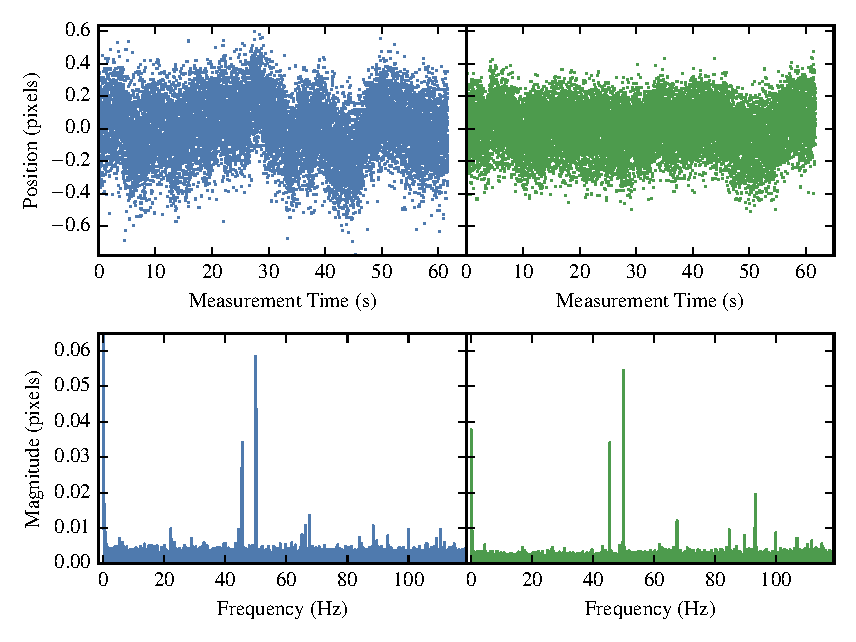
\includegraphics{part2/Figs/cw_beam_stability.pdf}
    \caption{Continuous electron beam.}
    \label{figure:cw_stability}
    \end{subfigure}

    \begin{subfigure}{\linewidth}
    \centering
    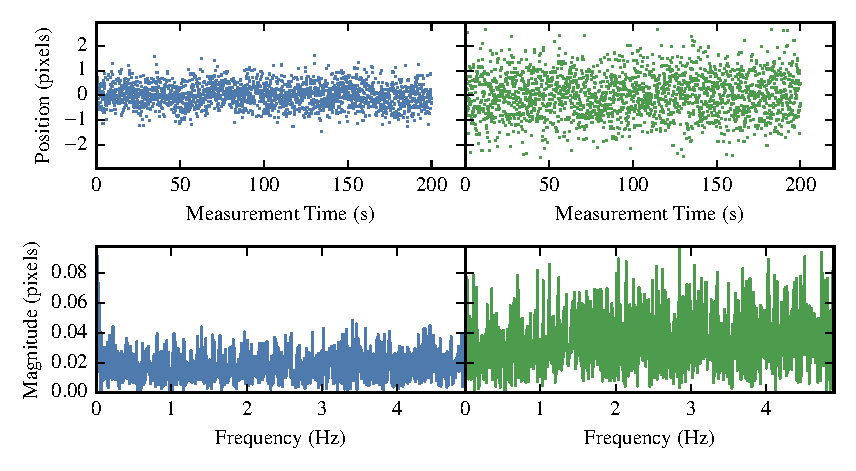
\includegraphics{part2/Figs/pulse_beam_stability.pdf}
    \caption{Pulsed electron beam.}
    \label{figure:pulse_stability}
    \end{subfigure}
    \caption[Beam stability for continuous and pulsed operation.]{Beam position and position spectrum for $x$ (blue) and $y$ (green) directions for \gls{cw}-mode electrons (a) and pulse-mode electrons (b).
    Pulsed operation is limited to \unit[10]{Hz} and thus the spectrum is limited to \unit[5]{Hz}. The continuous beam spectrum was limited to \unit[120]{Hz} by the camera framerate of \unit[240]{Hz}.}
    \label{figure:stability}
    % CW data and code at 2016.06.29
    % Pulsed data and code at 2016.06.17
\end{figure}

\subsection{Summary}

It was hoped that continuous mode would provide a viable alternative to normal pulsed operation with this iteration of the \gls{caeis} with better beam current and stability.
An increase in the time-averaged beam current of approximately a factor of six is possible, compared to pulsed mode, by increasing the atomic flux and intensity of the blue ionisation laser.
The fast switching on and off of the \gls{mot} and Zeeman slower magnetic coils were eliminated as a primary candidate for the electron beam instabilities as the magnitude of the drift was more or less the same with pulsed and \gls{cw} mode.

The investigations in this section indicate that, with the current apparatus, continuous mode is able to provide an increase in beam current but no increase in beam stability at the cost of no longer being able to produce ultrafast bunches.
The next generation of the \gls{caeis} now under construction will operate as a continuous ion source, capitalising on the beam current achievable by directly ionising the atom beam~\cite{mcculloch_heralded_2018}.

\section{Registration}\label{section:registration}

Instability in the beam path (see Section~\ref{section:stability}) resulted in the electron beam trajectory drifting from shot-to-shot.
When multi-shot averages were required the beam drift resulted in the beam being `smeared' when averaged.
It was necessary to `register' the images to prevent this smearing and this is demonstrated in Figures~\ref{figure:registration_examples} and \ref{figure:real_registration_examples}.

\begin{figure}
    \center
    %% Creator: Matplotlib, PGF backend
%%
%% To include the figure in your LaTeX document, write
%%   \input{<filename>.pgf}
%%
%% Make sure the required packages are loaded in your preamble
%%   \usepackage{pgf}
%%
%% Figures using additional raster images can only be included by \input if
%% they are in the same directory as the main LaTeX file. For loading figures
%% from other directories you can use the `import` package
%%   \usepackage{import}
%% and then include the figures with
%%   \import{<path to file>}{<filename>.pgf}
%%
%% Matplotlib used the following preamble
%%
\begingroup%
\makeatletter%
\begin{pgfpicture}%
\pgfpathrectangle{\pgfpointorigin}{\pgfqpoint{5.710000in}{5.710000in}}%
\pgfusepath{use as bounding box, clip}%
\begin{pgfscope}%
\pgfsetbuttcap%
\pgfsetmiterjoin%
\definecolor{currentfill}{rgb}{1.000000,1.000000,1.000000}%
\pgfsetfillcolor{currentfill}%
\pgfsetlinewidth{0.000000pt}%
\definecolor{currentstroke}{rgb}{1.000000,1.000000,1.000000}%
\pgfsetstrokecolor{currentstroke}%
\pgfsetdash{}{0pt}%
\pgfpathmoveto{\pgfqpoint{0.000000in}{0.000000in}}%
\pgfpathlineto{\pgfqpoint{5.710000in}{0.000000in}}%
\pgfpathlineto{\pgfqpoint{5.710000in}{5.710000in}}%
\pgfpathlineto{\pgfqpoint{0.000000in}{5.710000in}}%
\pgfpathclose%
\pgfusepath{fill}%
\end{pgfscope}%
\begin{pgfscope}%
\pgfsetbuttcap%
\pgfsetmiterjoin%
\definecolor{currentfill}{rgb}{1.000000,1.000000,1.000000}%
\pgfsetfillcolor{currentfill}%
\pgfsetlinewidth{0.000000pt}%
\definecolor{currentstroke}{rgb}{0.000000,0.000000,0.000000}%
\pgfsetstrokecolor{currentstroke}%
\pgfsetstrokeopacity{0.000000}%
\pgfsetdash{}{0pt}%
\pgfpathmoveto{\pgfqpoint{0.216430in}{2.913778in}}%
\pgfpathlineto{\pgfqpoint{2.713570in}{2.913778in}}%
\pgfpathlineto{\pgfqpoint{2.713570in}{5.410919in}}%
\pgfpathlineto{\pgfqpoint{0.216430in}{5.410919in}}%
\pgfpathclose%
\pgfusepath{fill}%
\end{pgfscope}%
\begin{pgfscope}%
\pgfpathrectangle{\pgfqpoint{0.216430in}{2.913778in}}{\pgfqpoint{2.497141in}{2.497141in}} %
\pgfusepath{clip}%
\pgftext[at=\pgfqpoint{0.216430in}{2.913778in},left,bottom]{\pgfimage[interpolate=true,width=2.500000in,height=2.510000in]{registration_examples-img0.png}}%
\end{pgfscope}%
\begin{pgfscope}%
\pgfsetrectcap%
\pgfsetmiterjoin%
\pgfsetlinewidth{1.003750pt}%
\definecolor{currentstroke}{rgb}{0.000000,0.000000,0.000000}%
\pgfsetstrokecolor{currentstroke}%
\pgfsetdash{}{0pt}%
\pgfpathmoveto{\pgfqpoint{2.713570in}{2.913778in}}%
\pgfpathlineto{\pgfqpoint{2.713570in}{5.410919in}}%
\pgfusepath{stroke}%
\end{pgfscope}%
\begin{pgfscope}%
\pgfsetrectcap%
\pgfsetmiterjoin%
\pgfsetlinewidth{1.003750pt}%
\definecolor{currentstroke}{rgb}{0.000000,0.000000,0.000000}%
\pgfsetstrokecolor{currentstroke}%
\pgfsetdash{}{0pt}%
\pgfpathmoveto{\pgfqpoint{0.216430in}{2.913778in}}%
\pgfpathlineto{\pgfqpoint{2.713570in}{2.913778in}}%
\pgfusepath{stroke}%
\end{pgfscope}%
\begin{pgfscope}%
\pgfsetrectcap%
\pgfsetmiterjoin%
\pgfsetlinewidth{1.003750pt}%
\definecolor{currentstroke}{rgb}{0.000000,0.000000,0.000000}%
\pgfsetstrokecolor{currentstroke}%
\pgfsetdash{}{0pt}%
\pgfpathmoveto{\pgfqpoint{0.216430in}{2.913778in}}%
\pgfpathlineto{\pgfqpoint{0.216430in}{5.410919in}}%
\pgfusepath{stroke}%
\end{pgfscope}%
\begin{pgfscope}%
\pgfsetrectcap%
\pgfsetmiterjoin%
\pgfsetlinewidth{1.003750pt}%
\definecolor{currentstroke}{rgb}{0.000000,0.000000,0.000000}%
\pgfsetstrokecolor{currentstroke}%
\pgfsetdash{}{0pt}%
\pgfpathmoveto{\pgfqpoint{0.216430in}{5.410919in}}%
\pgfpathlineto{\pgfqpoint{2.713570in}{5.410919in}}%
\pgfusepath{stroke}%
\end{pgfscope}%
\begin{pgfscope}%
\pgftext[x=1.465000in,y=5.480364in,,base]{\fontsize{12.000000}{14.400000}\selectfont Single-Shot}%
\end{pgfscope}%
\begin{pgfscope}%
\pgfsetbuttcap%
\pgfsetmiterjoin%
\definecolor{currentfill}{rgb}{1.000000,1.000000,1.000000}%
\pgfsetfillcolor{currentfill}%
\pgfsetlinewidth{0.000000pt}%
\definecolor{currentstroke}{rgb}{0.000000,0.000000,0.000000}%
\pgfsetstrokecolor{currentstroke}%
\pgfsetstrokeopacity{0.000000}%
\pgfsetdash{}{0pt}%
\pgfpathmoveto{\pgfqpoint{2.996430in}{2.913778in}}%
\pgfpathlineto{\pgfqpoint{5.493570in}{2.913778in}}%
\pgfpathlineto{\pgfqpoint{5.493570in}{5.410919in}}%
\pgfpathlineto{\pgfqpoint{2.996430in}{5.410919in}}%
\pgfpathclose%
\pgfusepath{fill}%
\end{pgfscope}%
\begin{pgfscope}%
\pgfpathrectangle{\pgfqpoint{2.996430in}{2.913778in}}{\pgfqpoint{2.497141in}{2.497141in}} %
\pgfusepath{clip}%
\pgftext[at=\pgfqpoint{2.996430in}{2.913778in},left,bottom]{\pgfimage[interpolate=true,width=2.500000in,height=2.510000in]{registration_examples-img1.png}}%
\end{pgfscope}%
\begin{pgfscope}%
\pgfsetrectcap%
\pgfsetmiterjoin%
\pgfsetlinewidth{1.003750pt}%
\definecolor{currentstroke}{rgb}{0.000000,0.000000,0.000000}%
\pgfsetstrokecolor{currentstroke}%
\pgfsetdash{}{0pt}%
\pgfpathmoveto{\pgfqpoint{5.493570in}{2.913778in}}%
\pgfpathlineto{\pgfqpoint{5.493570in}{5.410919in}}%
\pgfusepath{stroke}%
\end{pgfscope}%
\begin{pgfscope}%
\pgfsetrectcap%
\pgfsetmiterjoin%
\pgfsetlinewidth{1.003750pt}%
\definecolor{currentstroke}{rgb}{0.000000,0.000000,0.000000}%
\pgfsetstrokecolor{currentstroke}%
\pgfsetdash{}{0pt}%
\pgfpathmoveto{\pgfqpoint{2.996430in}{2.913778in}}%
\pgfpathlineto{\pgfqpoint{5.493570in}{2.913778in}}%
\pgfusepath{stroke}%
\end{pgfscope}%
\begin{pgfscope}%
\pgfsetrectcap%
\pgfsetmiterjoin%
\pgfsetlinewidth{1.003750pt}%
\definecolor{currentstroke}{rgb}{0.000000,0.000000,0.000000}%
\pgfsetstrokecolor{currentstroke}%
\pgfsetdash{}{0pt}%
\pgfpathmoveto{\pgfqpoint{2.996430in}{2.913778in}}%
\pgfpathlineto{\pgfqpoint{2.996430in}{5.410919in}}%
\pgfusepath{stroke}%
\end{pgfscope}%
\begin{pgfscope}%
\pgfsetrectcap%
\pgfsetmiterjoin%
\pgfsetlinewidth{1.003750pt}%
\definecolor{currentstroke}{rgb}{0.000000,0.000000,0.000000}%
\pgfsetstrokecolor{currentstroke}%
\pgfsetdash{}{0pt}%
\pgfpathmoveto{\pgfqpoint{2.996430in}{5.410919in}}%
\pgfpathlineto{\pgfqpoint{5.493570in}{5.410919in}}%
\pgfusepath{stroke}%
\end{pgfscope}%
\begin{pgfscope}%
\pgftext[x=4.245000in,y=5.480364in,,base]{\fontsize{12.000000}{14.400000}\selectfont Average}%
\end{pgfscope}%
\begin{pgfscope}%
\pgfsetbuttcap%
\pgfsetmiterjoin%
\definecolor{currentfill}{rgb}{1.000000,1.000000,1.000000}%
\pgfsetfillcolor{currentfill}%
\pgfsetlinewidth{0.000000pt}%
\definecolor{currentstroke}{rgb}{0.000000,0.000000,0.000000}%
\pgfsetstrokecolor{currentstroke}%
\pgfsetstrokeopacity{0.000000}%
\pgfsetdash{}{0pt}%
\pgfpathmoveto{\pgfqpoint{0.216430in}{0.150000in}}%
\pgfpathlineto{\pgfqpoint{2.713570in}{0.150000in}}%
\pgfpathlineto{\pgfqpoint{2.713570in}{2.647141in}}%
\pgfpathlineto{\pgfqpoint{0.216430in}{2.647141in}}%
\pgfpathclose%
\pgfusepath{fill}%
\end{pgfscope}%
\begin{pgfscope}%
\pgfpathrectangle{\pgfqpoint{0.216430in}{0.150000in}}{\pgfqpoint{2.497141in}{2.497141in}} %
\pgfusepath{clip}%
\pgftext[at=\pgfqpoint{0.216430in}{0.150000in},left,bottom]{\pgfimage[interpolate=true,width=2.500000in,height=2.510000in]{registration_examples-img2.png}}%
\end{pgfscope}%
\begin{pgfscope}%
\pgfsetrectcap%
\pgfsetmiterjoin%
\pgfsetlinewidth{1.003750pt}%
\definecolor{currentstroke}{rgb}{0.000000,0.000000,0.000000}%
\pgfsetstrokecolor{currentstroke}%
\pgfsetdash{}{0pt}%
\pgfpathmoveto{\pgfqpoint{2.713570in}{0.150000in}}%
\pgfpathlineto{\pgfqpoint{2.713570in}{2.647141in}}%
\pgfusepath{stroke}%
\end{pgfscope}%
\begin{pgfscope}%
\pgfsetrectcap%
\pgfsetmiterjoin%
\pgfsetlinewidth{1.003750pt}%
\definecolor{currentstroke}{rgb}{0.000000,0.000000,0.000000}%
\pgfsetstrokecolor{currentstroke}%
\pgfsetdash{}{0pt}%
\pgfpathmoveto{\pgfqpoint{0.216430in}{0.150000in}}%
\pgfpathlineto{\pgfqpoint{2.713570in}{0.150000in}}%
\pgfusepath{stroke}%
\end{pgfscope}%
\begin{pgfscope}%
\pgfsetrectcap%
\pgfsetmiterjoin%
\pgfsetlinewidth{1.003750pt}%
\definecolor{currentstroke}{rgb}{0.000000,0.000000,0.000000}%
\pgfsetstrokecolor{currentstroke}%
\pgfsetdash{}{0pt}%
\pgfpathmoveto{\pgfqpoint{0.216430in}{0.150000in}}%
\pgfpathlineto{\pgfqpoint{0.216430in}{2.647141in}}%
\pgfusepath{stroke}%
\end{pgfscope}%
\begin{pgfscope}%
\pgfsetrectcap%
\pgfsetmiterjoin%
\pgfsetlinewidth{1.003750pt}%
\definecolor{currentstroke}{rgb}{0.000000,0.000000,0.000000}%
\pgfsetstrokecolor{currentstroke}%
\pgfsetdash{}{0pt}%
\pgfpathmoveto{\pgfqpoint{0.216430in}{2.647141in}}%
\pgfpathlineto{\pgfqpoint{2.713570in}{2.647141in}}%
\pgfusepath{stroke}%
\end{pgfscope}%
\begin{pgfscope}%
\pgftext[x=1.465000in,y=2.716585in,,base]{\fontsize{12.000000}{14.400000}\selectfont Slipped}%
\end{pgfscope}%
\begin{pgfscope}%
\pgfsetbuttcap%
\pgfsetmiterjoin%
\definecolor{currentfill}{rgb}{1.000000,1.000000,1.000000}%
\pgfsetfillcolor{currentfill}%
\pgfsetlinewidth{0.000000pt}%
\definecolor{currentstroke}{rgb}{0.000000,0.000000,0.000000}%
\pgfsetstrokecolor{currentstroke}%
\pgfsetstrokeopacity{0.000000}%
\pgfsetdash{}{0pt}%
\pgfpathmoveto{\pgfqpoint{2.996430in}{0.150000in}}%
\pgfpathlineto{\pgfqpoint{5.493570in}{0.150000in}}%
\pgfpathlineto{\pgfqpoint{5.493570in}{2.647141in}}%
\pgfpathlineto{\pgfqpoint{2.996430in}{2.647141in}}%
\pgfpathclose%
\pgfusepath{fill}%
\end{pgfscope}%
\begin{pgfscope}%
\pgfpathrectangle{\pgfqpoint{2.996430in}{0.150000in}}{\pgfqpoint{2.497141in}{2.497141in}} %
\pgfusepath{clip}%
\pgftext[at=\pgfqpoint{2.996430in}{0.150000in},left,bottom]{\pgfimage[interpolate=true,width=2.500000in,height=2.510000in]{registration_examples-img3.png}}%
\end{pgfscope}%
\begin{pgfscope}%
\pgfsetrectcap%
\pgfsetmiterjoin%
\pgfsetlinewidth{1.003750pt}%
\definecolor{currentstroke}{rgb}{0.000000,0.000000,0.000000}%
\pgfsetstrokecolor{currentstroke}%
\pgfsetdash{}{0pt}%
\pgfpathmoveto{\pgfqpoint{5.493570in}{0.150000in}}%
\pgfpathlineto{\pgfqpoint{5.493570in}{2.647141in}}%
\pgfusepath{stroke}%
\end{pgfscope}%
\begin{pgfscope}%
\pgfsetrectcap%
\pgfsetmiterjoin%
\pgfsetlinewidth{1.003750pt}%
\definecolor{currentstroke}{rgb}{0.000000,0.000000,0.000000}%
\pgfsetstrokecolor{currentstroke}%
\pgfsetdash{}{0pt}%
\pgfpathmoveto{\pgfqpoint{2.996430in}{0.150000in}}%
\pgfpathlineto{\pgfqpoint{5.493570in}{0.150000in}}%
\pgfusepath{stroke}%
\end{pgfscope}%
\begin{pgfscope}%
\pgfsetrectcap%
\pgfsetmiterjoin%
\pgfsetlinewidth{1.003750pt}%
\definecolor{currentstroke}{rgb}{0.000000,0.000000,0.000000}%
\pgfsetstrokecolor{currentstroke}%
\pgfsetdash{}{0pt}%
\pgfpathmoveto{\pgfqpoint{2.996430in}{0.150000in}}%
\pgfpathlineto{\pgfqpoint{2.996430in}{2.647141in}}%
\pgfusepath{stroke}%
\end{pgfscope}%
\begin{pgfscope}%
\pgfsetrectcap%
\pgfsetmiterjoin%
\pgfsetlinewidth{1.003750pt}%
\definecolor{currentstroke}{rgb}{0.000000,0.000000,0.000000}%
\pgfsetstrokecolor{currentstroke}%
\pgfsetdash{}{0pt}%
\pgfpathmoveto{\pgfqpoint{2.996430in}{2.647141in}}%
\pgfpathlineto{\pgfqpoint{5.493570in}{2.647141in}}%
\pgfusepath{stroke}%
\end{pgfscope}%
\begin{pgfscope}%
\pgftext[x=4.245000in,y=2.716585in,,base]{\fontsize{12.000000}{14.400000}\selectfont Registered}%
\end{pgfscope}%
\end{pgfpicture}%
\makeatother%
\endgroup%

    \caption[Contrived image registration example.]{A demonstration of the importance of the image registration technique using a contrived example of slipping. \emph{Single-Shot} is a single image from a prototype-pepperpot data set of 1000 images. \emph{Average} is the simple average of all 1000 images. \emph{Slipped} is a contrived demonstration of slipping; there is an additional set of beamlets visible at the top of the image. \emph{Registration} is a successful registration where a shot-to-shot limit to drift was enforced. All the images are independently log scaled.}
    \label{figure:registration_examples}
    % Data and code in 2016.10.27
\end{figure}

\begin{figure}
    \center
    %% Creator: Matplotlib, PGF backend
%%
%% To include the figure in your LaTeX document, write
%%   \input{<filename>.pgf}
%%
%% Make sure the required packages are loaded in your preamble
%%   \usepackage{pgf}
%%
%% Figures using additional raster images can only be included by \input if
%% they are in the same directory as the main LaTeX file. For loading figures
%% from other directories you can use the `import` package
%%   \usepackage{import}
%% and then include the figures with
%%   \import{<path to file>}{<filename>.pgf}
%%
%% Matplotlib used the following preamble
%%
\begingroup%
\makeatletter%
\begin{pgfpicture}%
\pgfpathrectangle{\pgfpointorigin}{\pgfqpoint{5.710000in}{5.710000in}}%
\pgfusepath{use as bounding box, clip}%
\begin{pgfscope}%
\pgfsetbuttcap%
\pgfsetmiterjoin%
\definecolor{currentfill}{rgb}{1.000000,1.000000,1.000000}%
\pgfsetfillcolor{currentfill}%
\pgfsetlinewidth{0.000000pt}%
\definecolor{currentstroke}{rgb}{1.000000,1.000000,1.000000}%
\pgfsetstrokecolor{currentstroke}%
\pgfsetdash{}{0pt}%
\pgfpathmoveto{\pgfqpoint{0.000000in}{0.000000in}}%
\pgfpathlineto{\pgfqpoint{5.710000in}{0.000000in}}%
\pgfpathlineto{\pgfqpoint{5.710000in}{5.710000in}}%
\pgfpathlineto{\pgfqpoint{0.000000in}{5.710000in}}%
\pgfpathclose%
\pgfusepath{fill}%
\end{pgfscope}%
\begin{pgfscope}%
\pgftext[x=3.143906in,y=0.459462in,,top]{\rmfamily\fontsize{10.000000}{12.000000}\selectfont Vertical Position (mm)}%
\end{pgfscope}%
\begin{pgfscope}%
\pgfsetbuttcap%
\pgfsetmiterjoin%
\definecolor{currentfill}{rgb}{1.000000,1.000000,1.000000}%
\pgfsetfillcolor{currentfill}%
\pgfsetlinewidth{0.000000pt}%
\definecolor{currentstroke}{rgb}{0.000000,0.000000,0.000000}%
\pgfsetstrokecolor{currentstroke}%
\pgfsetstrokeopacity{0.000000}%
\pgfsetdash{}{0pt}%
\pgfpathmoveto{\pgfqpoint{0.727812in}{4.631530in}}%
\pgfpathlineto{\pgfqpoint{3.143906in}{4.631530in}}%
\pgfpathlineto{\pgfqpoint{3.143906in}{5.365556in}}%
\pgfpathlineto{\pgfqpoint{0.727812in}{5.365556in}}%
\pgfpathclose%
\pgfusepath{fill}%
\end{pgfscope}%
\begin{pgfscope}%
\pgfpathrectangle{\pgfqpoint{0.727812in}{4.631530in}}{\pgfqpoint{2.416094in}{0.734025in}} %
\pgfusepath{clip}%
\pgftext[at=\pgfqpoint{0.727812in}{4.631530in},left,bottom]{\pgfimage[interpolate=true,width=2.420000in,height=0.750000in]{streak_registration_examples-img0.png}}%
\end{pgfscope}%
\begin{pgfscope}%
\pgfsetrectcap%
\pgfsetmiterjoin%
\pgfsetlinewidth{1.003750pt}%
\definecolor{currentstroke}{rgb}{0.000000,0.000000,0.000000}%
\pgfsetstrokecolor{currentstroke}%
\pgfsetdash{}{0pt}%
\pgfpathmoveto{\pgfqpoint{0.727812in}{5.365556in}}%
\pgfpathlineto{\pgfqpoint{3.143906in}{5.365556in}}%
\pgfusepath{stroke}%
\end{pgfscope}%
\begin{pgfscope}%
\pgfsetrectcap%
\pgfsetmiterjoin%
\pgfsetlinewidth{1.003750pt}%
\definecolor{currentstroke}{rgb}{0.000000,0.000000,0.000000}%
\pgfsetstrokecolor{currentstroke}%
\pgfsetdash{}{0pt}%
\pgfpathmoveto{\pgfqpoint{0.727812in}{4.631530in}}%
\pgfpathlineto{\pgfqpoint{3.143906in}{4.631530in}}%
\pgfusepath{stroke}%
\end{pgfscope}%
\begin{pgfscope}%
\pgfsetrectcap%
\pgfsetmiterjoin%
\pgfsetlinewidth{1.003750pt}%
\definecolor{currentstroke}{rgb}{0.000000,0.000000,0.000000}%
\pgfsetstrokecolor{currentstroke}%
\pgfsetdash{}{0pt}%
\pgfpathmoveto{\pgfqpoint{0.727812in}{4.631530in}}%
\pgfpathlineto{\pgfqpoint{0.727812in}{5.365556in}}%
\pgfusepath{stroke}%
\end{pgfscope}%
\begin{pgfscope}%
\pgfsetrectcap%
\pgfsetmiterjoin%
\pgfsetlinewidth{1.003750pt}%
\definecolor{currentstroke}{rgb}{0.000000,0.000000,0.000000}%
\pgfsetstrokecolor{currentstroke}%
\pgfsetdash{}{0pt}%
\pgfpathmoveto{\pgfqpoint{3.143906in}{4.631530in}}%
\pgfpathlineto{\pgfqpoint{3.143906in}{5.365556in}}%
\pgfusepath{stroke}%
\end{pgfscope}%
\begin{pgfscope}%
\pgftext[x=1.935859in,y=5.435000in,,base]{\rmfamily\fontsize{12.000000}{14.400000}\selectfont Single-Shot}%
\end{pgfscope}%
\begin{pgfscope}%
\pgfsetbuttcap%
\pgfsetmiterjoin%
\definecolor{currentfill}{rgb}{1.000000,1.000000,1.000000}%
\pgfsetfillcolor{currentfill}%
\pgfsetlinewidth{0.000000pt}%
\definecolor{currentstroke}{rgb}{0.000000,0.000000,0.000000}%
\pgfsetstrokecolor{currentstroke}%
\pgfsetstrokeopacity{0.000000}%
\pgfsetdash{}{0pt}%
\pgfpathmoveto{\pgfqpoint{0.727812in}{3.163480in}}%
\pgfpathlineto{\pgfqpoint{3.143906in}{3.163480in}}%
\pgfpathlineto{\pgfqpoint{3.143906in}{4.631530in}}%
\pgfpathlineto{\pgfqpoint{0.727812in}{4.631530in}}%
\pgfpathclose%
\pgfusepath{fill}%
\end{pgfscope}%
\begin{pgfscope}%
\pgfpathrectangle{\pgfqpoint{0.727812in}{3.163480in}}{\pgfqpoint{2.416094in}{1.468050in}} %
\pgfusepath{clip}%
\pgfsetrectcap%
\pgfsetroundjoin%
\pgfsetlinewidth{1.003750pt}%
\definecolor{currentstroke}{rgb}{0.309804,0.478431,0.682353}%
\pgfsetstrokecolor{currentstroke}%
\pgfsetdash{}{0pt}%
\pgfpathmoveto{\pgfqpoint{0.717812in}{3.235961in}}%
\pgfpathlineto{\pgfqpoint{0.728445in}{3.229623in}}%
\pgfpathlineto{\pgfqpoint{0.741088in}{3.250824in}}%
\pgfpathlineto{\pgfqpoint{0.753731in}{3.207259in}}%
\pgfpathlineto{\pgfqpoint{0.766374in}{3.222817in}}%
\pgfpathlineto{\pgfqpoint{0.779017in}{3.249459in}}%
\pgfpathlineto{\pgfqpoint{0.791660in}{3.196183in}}%
\pgfpathlineto{\pgfqpoint{0.804303in}{3.191081in}}%
\pgfpathlineto{\pgfqpoint{0.816946in}{3.239287in}}%
\pgfpathlineto{\pgfqpoint{0.829589in}{3.241361in}}%
\pgfpathlineto{\pgfqpoint{0.842232in}{3.200169in}}%
\pgfpathlineto{\pgfqpoint{0.854876in}{3.240849in}}%
\pgfpathlineto{\pgfqpoint{0.867519in}{3.266503in}}%
\pgfpathlineto{\pgfqpoint{0.880162in}{3.236294in}}%
\pgfpathlineto{\pgfqpoint{0.892805in}{3.269625in}}%
\pgfpathlineto{\pgfqpoint{0.905448in}{3.240378in}}%
\pgfpathlineto{\pgfqpoint{0.918091in}{3.263887in}}%
\pgfpathlineto{\pgfqpoint{0.930734in}{3.239537in}}%
\pgfpathlineto{\pgfqpoint{0.943377in}{3.228572in}}%
\pgfpathlineto{\pgfqpoint{0.956020in}{3.297129in}}%
\pgfpathlineto{\pgfqpoint{0.968663in}{3.279248in}}%
\pgfpathlineto{\pgfqpoint{0.981306in}{3.244002in}}%
\pgfpathlineto{\pgfqpoint{0.993949in}{3.280854in}}%
\pgfpathlineto{\pgfqpoint{1.006593in}{3.246950in}}%
\pgfpathlineto{\pgfqpoint{1.019236in}{3.262109in}}%
\pgfpathlineto{\pgfqpoint{1.031879in}{3.309866in}}%
\pgfpathlineto{\pgfqpoint{1.044522in}{3.254045in}}%
\pgfpathlineto{\pgfqpoint{1.057165in}{3.305856in}}%
\pgfpathlineto{\pgfqpoint{1.069808in}{3.372474in}}%
\pgfpathlineto{\pgfqpoint{1.082451in}{3.382131in}}%
\pgfpathlineto{\pgfqpoint{1.095094in}{3.346001in}}%
\pgfpathlineto{\pgfqpoint{1.107737in}{3.343276in}}%
\pgfpathlineto{\pgfqpoint{1.120380in}{3.386913in}}%
\pgfpathlineto{\pgfqpoint{1.133023in}{3.356614in}}%
\pgfpathlineto{\pgfqpoint{1.145666in}{3.350578in}}%
\pgfpathlineto{\pgfqpoint{1.158310in}{3.354010in}}%
\pgfpathlineto{\pgfqpoint{1.170953in}{3.342746in}}%
\pgfpathlineto{\pgfqpoint{1.183596in}{3.314877in}}%
\pgfpathlineto{\pgfqpoint{1.196239in}{3.342491in}}%
\pgfpathlineto{\pgfqpoint{1.208882in}{3.360580in}}%
\pgfpathlineto{\pgfqpoint{1.221525in}{3.342487in}}%
\pgfpathlineto{\pgfqpoint{1.246811in}{3.441586in}}%
\pgfpathlineto{\pgfqpoint{1.259454in}{3.440679in}}%
\pgfpathlineto{\pgfqpoint{1.272097in}{3.538661in}}%
\pgfpathlineto{\pgfqpoint{1.284740in}{3.691062in}}%
\pgfpathlineto{\pgfqpoint{1.297384in}{3.931921in}}%
\pgfpathlineto{\pgfqpoint{1.310027in}{4.031381in}}%
\pgfpathlineto{\pgfqpoint{1.322670in}{4.092211in}}%
\pgfpathlineto{\pgfqpoint{1.335313in}{4.021932in}}%
\pgfpathlineto{\pgfqpoint{1.347956in}{3.932258in}}%
\pgfpathlineto{\pgfqpoint{1.360599in}{3.816817in}}%
\pgfpathlineto{\pgfqpoint{1.373242in}{3.651509in}}%
\pgfpathlineto{\pgfqpoint{1.398528in}{3.449031in}}%
\pgfpathlineto{\pgfqpoint{1.411171in}{3.529741in}}%
\pgfpathlineto{\pgfqpoint{1.423814in}{3.487962in}}%
\pgfpathlineto{\pgfqpoint{1.436457in}{3.417213in}}%
\pgfpathlineto{\pgfqpoint{1.461744in}{3.469951in}}%
\pgfpathlineto{\pgfqpoint{1.474387in}{3.533352in}}%
\pgfpathlineto{\pgfqpoint{1.487030in}{3.608838in}}%
\pgfpathlineto{\pgfqpoint{1.499673in}{3.710843in}}%
\pgfpathlineto{\pgfqpoint{1.512316in}{3.788717in}}%
\pgfpathlineto{\pgfqpoint{1.537602in}{4.260046in}}%
\pgfpathlineto{\pgfqpoint{1.550245in}{4.435466in}}%
\pgfpathlineto{\pgfqpoint{1.562888in}{4.238166in}}%
\pgfpathlineto{\pgfqpoint{1.575531in}{3.892832in}}%
\pgfpathlineto{\pgfqpoint{1.588175in}{3.686273in}}%
\pgfpathlineto{\pgfqpoint{1.600818in}{3.562517in}}%
\pgfpathlineto{\pgfqpoint{1.613461in}{3.500655in}}%
\pgfpathlineto{\pgfqpoint{1.626104in}{3.527499in}}%
\pgfpathlineto{\pgfqpoint{1.638747in}{3.491186in}}%
\pgfpathlineto{\pgfqpoint{1.651390in}{3.490386in}}%
\pgfpathlineto{\pgfqpoint{1.664033in}{3.506564in}}%
\pgfpathlineto{\pgfqpoint{1.676676in}{3.491022in}}%
\pgfpathlineto{\pgfqpoint{1.689319in}{3.607795in}}%
\pgfpathlineto{\pgfqpoint{1.701962in}{3.713200in}}%
\pgfpathlineto{\pgfqpoint{1.714605in}{3.967269in}}%
\pgfpathlineto{\pgfqpoint{1.727248in}{4.299989in}}%
\pgfpathlineto{\pgfqpoint{1.739892in}{4.458664in}}%
\pgfpathlineto{\pgfqpoint{1.752535in}{4.251914in}}%
\pgfpathlineto{\pgfqpoint{1.765178in}{3.962990in}}%
\pgfpathlineto{\pgfqpoint{1.777821in}{3.707136in}}%
\pgfpathlineto{\pgfqpoint{1.790464in}{3.572545in}}%
\pgfpathlineto{\pgfqpoint{1.815750in}{3.484056in}}%
\pgfpathlineto{\pgfqpoint{1.828393in}{3.479840in}}%
\pgfpathlineto{\pgfqpoint{1.841036in}{3.460603in}}%
\pgfpathlineto{\pgfqpoint{1.853679in}{3.384249in}}%
\pgfpathlineto{\pgfqpoint{1.866322in}{3.423801in}}%
\pgfpathlineto{\pgfqpoint{1.878965in}{3.405909in}}%
\pgfpathlineto{\pgfqpoint{1.891609in}{3.410524in}}%
\pgfpathlineto{\pgfqpoint{1.904252in}{3.417215in}}%
\pgfpathlineto{\pgfqpoint{1.916895in}{3.460045in}}%
\pgfpathlineto{\pgfqpoint{1.929538in}{3.528941in}}%
\pgfpathlineto{\pgfqpoint{1.942181in}{3.608470in}}%
\pgfpathlineto{\pgfqpoint{1.954824in}{3.726546in}}%
\pgfpathlineto{\pgfqpoint{1.967467in}{3.927504in}}%
\pgfpathlineto{\pgfqpoint{1.980110in}{4.038163in}}%
\pgfpathlineto{\pgfqpoint{2.005396in}{3.608346in}}%
\pgfpathlineto{\pgfqpoint{2.018039in}{3.469464in}}%
\pgfpathlineto{\pgfqpoint{2.030683in}{3.429301in}}%
\pgfpathlineto{\pgfqpoint{2.043326in}{3.418915in}}%
\pgfpathlineto{\pgfqpoint{2.055969in}{3.363095in}}%
\pgfpathlineto{\pgfqpoint{2.068612in}{3.328442in}}%
\pgfpathlineto{\pgfqpoint{2.081255in}{3.357912in}}%
\pgfpathlineto{\pgfqpoint{2.093898in}{3.325277in}}%
\pgfpathlineto{\pgfqpoint{2.106541in}{3.346224in}}%
\pgfpathlineto{\pgfqpoint{2.119184in}{3.320234in}}%
\pgfpathlineto{\pgfqpoint{2.131827in}{3.365508in}}%
\pgfpathlineto{\pgfqpoint{2.144470in}{3.422073in}}%
\pgfpathlineto{\pgfqpoint{2.169756in}{3.508482in}}%
\pgfpathlineto{\pgfqpoint{2.182400in}{3.532780in}}%
\pgfpathlineto{\pgfqpoint{2.195043in}{3.615785in}}%
\pgfpathlineto{\pgfqpoint{2.207686in}{3.639377in}}%
\pgfpathlineto{\pgfqpoint{2.220329in}{3.562605in}}%
\pgfpathlineto{\pgfqpoint{2.232972in}{3.412777in}}%
\pgfpathlineto{\pgfqpoint{2.245615in}{3.378141in}}%
\pgfpathlineto{\pgfqpoint{2.258258in}{3.366874in}}%
\pgfpathlineto{\pgfqpoint{2.270901in}{3.289849in}}%
\pgfpathlineto{\pgfqpoint{2.283544in}{3.310479in}}%
\pgfpathlineto{\pgfqpoint{2.296187in}{3.341898in}}%
\pgfpathlineto{\pgfqpoint{2.308830in}{3.292076in}}%
\pgfpathlineto{\pgfqpoint{2.321474in}{3.307669in}}%
\pgfpathlineto{\pgfqpoint{2.334117in}{3.320504in}}%
\pgfpathlineto{\pgfqpoint{2.346760in}{3.288094in}}%
\pgfpathlineto{\pgfqpoint{2.359403in}{3.288999in}}%
\pgfpathlineto{\pgfqpoint{2.372046in}{3.247326in}}%
\pgfpathlineto{\pgfqpoint{2.384689in}{3.292536in}}%
\pgfpathlineto{\pgfqpoint{2.397332in}{3.326209in}}%
\pgfpathlineto{\pgfqpoint{2.409975in}{3.350854in}}%
\pgfpathlineto{\pgfqpoint{2.435261in}{3.466115in}}%
\pgfpathlineto{\pgfqpoint{2.447904in}{3.451623in}}%
\pgfpathlineto{\pgfqpoint{2.460547in}{3.406406in}}%
\pgfpathlineto{\pgfqpoint{2.473191in}{3.323006in}}%
\pgfpathlineto{\pgfqpoint{2.485834in}{3.305243in}}%
\pgfpathlineto{\pgfqpoint{2.498477in}{3.268693in}}%
\pgfpathlineto{\pgfqpoint{2.511120in}{3.273410in}}%
\pgfpathlineto{\pgfqpoint{2.523763in}{3.234989in}}%
\pgfpathlineto{\pgfqpoint{2.536406in}{3.259598in}}%
\pgfpathlineto{\pgfqpoint{2.549049in}{3.252164in}}%
\pgfpathlineto{\pgfqpoint{2.561692in}{3.230210in}}%
\pgfpathlineto{\pgfqpoint{2.574335in}{3.226514in}}%
\pgfpathlineto{\pgfqpoint{2.586978in}{3.198153in}}%
\pgfpathlineto{\pgfqpoint{2.599621in}{3.222784in}}%
\pgfpathlineto{\pgfqpoint{2.612264in}{3.252360in}}%
\pgfpathlineto{\pgfqpoint{2.624908in}{3.207758in}}%
\pgfpathlineto{\pgfqpoint{2.637551in}{3.231271in}}%
\pgfpathlineto{\pgfqpoint{2.650194in}{3.231371in}}%
\pgfpathlineto{\pgfqpoint{2.662837in}{3.233665in}}%
\pgfpathlineto{\pgfqpoint{2.675480in}{3.240656in}}%
\pgfpathlineto{\pgfqpoint{2.688123in}{3.254183in}}%
\pgfpathlineto{\pgfqpoint{2.700766in}{3.192408in}}%
\pgfpathlineto{\pgfqpoint{2.713409in}{3.179565in}}%
\pgfpathlineto{\pgfqpoint{2.726052in}{3.233655in}}%
\pgfpathlineto{\pgfqpoint{2.738695in}{3.263104in}}%
\pgfpathlineto{\pgfqpoint{2.751338in}{3.219879in}}%
\pgfpathlineto{\pgfqpoint{2.763982in}{3.224533in}}%
\pgfpathlineto{\pgfqpoint{2.776625in}{3.213419in}}%
\pgfpathlineto{\pgfqpoint{2.789268in}{3.197460in}}%
\pgfpathlineto{\pgfqpoint{2.801911in}{3.163480in}}%
\pgfpathlineto{\pgfqpoint{2.814554in}{3.210106in}}%
\pgfpathlineto{\pgfqpoint{2.827197in}{3.223267in}}%
\pgfpathlineto{\pgfqpoint{2.839840in}{3.198662in}}%
\pgfpathlineto{\pgfqpoint{2.852483in}{3.241806in}}%
\pgfpathlineto{\pgfqpoint{2.865126in}{3.251478in}}%
\pgfpathlineto{\pgfqpoint{2.877769in}{3.185554in}}%
\pgfpathlineto{\pgfqpoint{2.903055in}{3.274562in}}%
\pgfpathlineto{\pgfqpoint{2.915699in}{3.258179in}}%
\pgfpathlineto{\pgfqpoint{2.928342in}{3.230370in}}%
\pgfpathlineto{\pgfqpoint{2.940985in}{3.194409in}}%
\pgfpathlineto{\pgfqpoint{2.953628in}{3.197151in}}%
\pgfpathlineto{\pgfqpoint{2.966271in}{3.201688in}}%
\pgfpathlineto{\pgfqpoint{2.978914in}{3.229966in}}%
\pgfpathlineto{\pgfqpoint{2.991557in}{3.172960in}}%
\pgfpathlineto{\pgfqpoint{3.004200in}{3.173785in}}%
\pgfpathlineto{\pgfqpoint{3.016843in}{3.231366in}}%
\pgfpathlineto{\pgfqpoint{3.029486in}{3.243154in}}%
\pgfpathlineto{\pgfqpoint{3.042129in}{3.229609in}}%
\pgfpathlineto{\pgfqpoint{3.054772in}{3.226657in}}%
\pgfpathlineto{\pgfqpoint{3.067416in}{3.260213in}}%
\pgfpathlineto{\pgfqpoint{3.080059in}{3.235657in}}%
\pgfpathlineto{\pgfqpoint{3.092702in}{3.220180in}}%
\pgfpathlineto{\pgfqpoint{3.105345in}{3.199056in}}%
\pgfpathlineto{\pgfqpoint{3.117988in}{3.194918in}}%
\pgfpathlineto{\pgfqpoint{3.130631in}{3.226263in}}%
\pgfpathlineto{\pgfqpoint{3.143274in}{3.211102in}}%
\pgfpathlineto{\pgfqpoint{3.153906in}{3.195082in}}%
\pgfpathlineto{\pgfqpoint{3.153906in}{3.195082in}}%
\pgfusepath{stroke}%
\end{pgfscope}%
\begin{pgfscope}%
\pgfsetrectcap%
\pgfsetmiterjoin%
\pgfsetlinewidth{1.003750pt}%
\definecolor{currentstroke}{rgb}{0.000000,0.000000,0.000000}%
\pgfsetstrokecolor{currentstroke}%
\pgfsetdash{}{0pt}%
\pgfpathmoveto{\pgfqpoint{0.727812in}{4.631530in}}%
\pgfpathlineto{\pgfqpoint{3.143906in}{4.631530in}}%
\pgfusepath{stroke}%
\end{pgfscope}%
\begin{pgfscope}%
\pgfsetrectcap%
\pgfsetmiterjoin%
\pgfsetlinewidth{1.003750pt}%
\definecolor{currentstroke}{rgb}{0.000000,0.000000,0.000000}%
\pgfsetstrokecolor{currentstroke}%
\pgfsetdash{}{0pt}%
\pgfpathmoveto{\pgfqpoint{0.727812in}{3.163480in}}%
\pgfpathlineto{\pgfqpoint{3.143906in}{3.163480in}}%
\pgfusepath{stroke}%
\end{pgfscope}%
\begin{pgfscope}%
\pgfsetrectcap%
\pgfsetmiterjoin%
\pgfsetlinewidth{1.003750pt}%
\definecolor{currentstroke}{rgb}{0.000000,0.000000,0.000000}%
\pgfsetstrokecolor{currentstroke}%
\pgfsetdash{}{0pt}%
\pgfpathmoveto{\pgfqpoint{0.727812in}{3.163480in}}%
\pgfpathlineto{\pgfqpoint{0.727812in}{4.631530in}}%
\pgfusepath{stroke}%
\end{pgfscope}%
\begin{pgfscope}%
\pgfsetrectcap%
\pgfsetmiterjoin%
\pgfsetlinewidth{1.003750pt}%
\definecolor{currentstroke}{rgb}{0.000000,0.000000,0.000000}%
\pgfsetstrokecolor{currentstroke}%
\pgfsetdash{}{0pt}%
\pgfpathmoveto{\pgfqpoint{3.143906in}{3.163480in}}%
\pgfpathlineto{\pgfqpoint{3.143906in}{4.631530in}}%
\pgfusepath{stroke}%
\end{pgfscope}%
\begin{pgfscope}%
\pgfsetbuttcap%
\pgfsetroundjoin%
\definecolor{currentfill}{rgb}{0.000000,0.000000,0.000000}%
\pgfsetfillcolor{currentfill}%
\pgfsetlinewidth{0.501875pt}%
\definecolor{currentstroke}{rgb}{0.000000,0.000000,0.000000}%
\pgfsetstrokecolor{currentstroke}%
\pgfsetdash{}{0pt}%
\pgfsys@defobject{currentmarker}{\pgfqpoint{0.000000in}{0.000000in}}{\pgfqpoint{0.000000in}{0.055556in}}{%
\pgfpathmoveto{\pgfqpoint{0.000000in}{0.000000in}}%
\pgfpathlineto{\pgfqpoint{0.000000in}{0.055556in}}%
\pgfusepath{stroke,fill}%
}%
\begin{pgfscope}%
\pgfsys@transformshift{1.006593in}{3.163480in}%
\pgfsys@useobject{currentmarker}{}%
\end{pgfscope}%
\end{pgfscope}%
\begin{pgfscope}%
\pgfsetbuttcap%
\pgfsetroundjoin%
\definecolor{currentfill}{rgb}{0.000000,0.000000,0.000000}%
\pgfsetfillcolor{currentfill}%
\pgfsetlinewidth{0.501875pt}%
\definecolor{currentstroke}{rgb}{0.000000,0.000000,0.000000}%
\pgfsetstrokecolor{currentstroke}%
\pgfsetdash{}{0pt}%
\pgfsys@defobject{currentmarker}{\pgfqpoint{0.000000in}{-0.055556in}}{\pgfqpoint{0.000000in}{0.000000in}}{%
\pgfpathmoveto{\pgfqpoint{0.000000in}{0.000000in}}%
\pgfpathlineto{\pgfqpoint{0.000000in}{-0.055556in}}%
\pgfusepath{stroke,fill}%
}%
\begin{pgfscope}%
\pgfsys@transformshift{1.006593in}{4.631530in}%
\pgfsys@useobject{currentmarker}{}%
\end{pgfscope}%
\end{pgfscope}%
\begin{pgfscope}%
\pgfsetbuttcap%
\pgfsetroundjoin%
\definecolor{currentfill}{rgb}{0.000000,0.000000,0.000000}%
\pgfsetfillcolor{currentfill}%
\pgfsetlinewidth{0.501875pt}%
\definecolor{currentstroke}{rgb}{0.000000,0.000000,0.000000}%
\pgfsetstrokecolor{currentstroke}%
\pgfsetdash{}{0pt}%
\pgfsys@defobject{currentmarker}{\pgfqpoint{0.000000in}{0.000000in}}{\pgfqpoint{0.000000in}{0.055556in}}{%
\pgfpathmoveto{\pgfqpoint{0.000000in}{0.000000in}}%
\pgfpathlineto{\pgfqpoint{0.000000in}{0.055556in}}%
\pgfusepath{stroke,fill}%
}%
\begin{pgfscope}%
\pgfsys@transformshift{1.935859in}{3.163480in}%
\pgfsys@useobject{currentmarker}{}%
\end{pgfscope}%
\end{pgfscope}%
\begin{pgfscope}%
\pgfsetbuttcap%
\pgfsetroundjoin%
\definecolor{currentfill}{rgb}{0.000000,0.000000,0.000000}%
\pgfsetfillcolor{currentfill}%
\pgfsetlinewidth{0.501875pt}%
\definecolor{currentstroke}{rgb}{0.000000,0.000000,0.000000}%
\pgfsetstrokecolor{currentstroke}%
\pgfsetdash{}{0pt}%
\pgfsys@defobject{currentmarker}{\pgfqpoint{0.000000in}{-0.055556in}}{\pgfqpoint{0.000000in}{0.000000in}}{%
\pgfpathmoveto{\pgfqpoint{0.000000in}{0.000000in}}%
\pgfpathlineto{\pgfqpoint{0.000000in}{-0.055556in}}%
\pgfusepath{stroke,fill}%
}%
\begin{pgfscope}%
\pgfsys@transformshift{1.935859in}{4.631530in}%
\pgfsys@useobject{currentmarker}{}%
\end{pgfscope}%
\end{pgfscope}%
\begin{pgfscope}%
\pgfsetbuttcap%
\pgfsetroundjoin%
\definecolor{currentfill}{rgb}{0.000000,0.000000,0.000000}%
\pgfsetfillcolor{currentfill}%
\pgfsetlinewidth{0.501875pt}%
\definecolor{currentstroke}{rgb}{0.000000,0.000000,0.000000}%
\pgfsetstrokecolor{currentstroke}%
\pgfsetdash{}{0pt}%
\pgfsys@defobject{currentmarker}{\pgfqpoint{0.000000in}{0.000000in}}{\pgfqpoint{0.000000in}{0.055556in}}{%
\pgfpathmoveto{\pgfqpoint{0.000000in}{0.000000in}}%
\pgfpathlineto{\pgfqpoint{0.000000in}{0.055556in}}%
\pgfusepath{stroke,fill}%
}%
\begin{pgfscope}%
\pgfsys@transformshift{2.865126in}{3.163480in}%
\pgfsys@useobject{currentmarker}{}%
\end{pgfscope}%
\end{pgfscope}%
\begin{pgfscope}%
\pgfsetbuttcap%
\pgfsetroundjoin%
\definecolor{currentfill}{rgb}{0.000000,0.000000,0.000000}%
\pgfsetfillcolor{currentfill}%
\pgfsetlinewidth{0.501875pt}%
\definecolor{currentstroke}{rgb}{0.000000,0.000000,0.000000}%
\pgfsetstrokecolor{currentstroke}%
\pgfsetdash{}{0pt}%
\pgfsys@defobject{currentmarker}{\pgfqpoint{0.000000in}{-0.055556in}}{\pgfqpoint{0.000000in}{0.000000in}}{%
\pgfpathmoveto{\pgfqpoint{0.000000in}{0.000000in}}%
\pgfpathlineto{\pgfqpoint{0.000000in}{-0.055556in}}%
\pgfusepath{stroke,fill}%
}%
\begin{pgfscope}%
\pgfsys@transformshift{2.865126in}{4.631530in}%
\pgfsys@useobject{currentmarker}{}%
\end{pgfscope}%
\end{pgfscope}%
\begin{pgfscope}%
\pgfsetbuttcap%
\pgfsetroundjoin%
\definecolor{currentfill}{rgb}{0.000000,0.000000,0.000000}%
\pgfsetfillcolor{currentfill}%
\pgfsetlinewidth{0.501875pt}%
\definecolor{currentstroke}{rgb}{0.000000,0.000000,0.000000}%
\pgfsetstrokecolor{currentstroke}%
\pgfsetdash{}{0pt}%
\pgfsys@defobject{currentmarker}{\pgfqpoint{0.000000in}{0.000000in}}{\pgfqpoint{0.055556in}{0.000000in}}{%
\pgfpathmoveto{\pgfqpoint{0.000000in}{0.000000in}}%
\pgfpathlineto{\pgfqpoint{0.055556in}{0.000000in}}%
\pgfusepath{stroke,fill}%
}%
\begin{pgfscope}%
\pgfsys@transformshift{0.727812in}{3.163480in}%
\pgfsys@useobject{currentmarker}{}%
\end{pgfscope}%
\end{pgfscope}%
\begin{pgfscope}%
\pgfsetbuttcap%
\pgfsetroundjoin%
\definecolor{currentfill}{rgb}{0.000000,0.000000,0.000000}%
\pgfsetfillcolor{currentfill}%
\pgfsetlinewidth{0.501875pt}%
\definecolor{currentstroke}{rgb}{0.000000,0.000000,0.000000}%
\pgfsetstrokecolor{currentstroke}%
\pgfsetdash{}{0pt}%
\pgfsys@defobject{currentmarker}{\pgfqpoint{-0.055556in}{0.000000in}}{\pgfqpoint{0.000000in}{0.000000in}}{%
\pgfpathmoveto{\pgfqpoint{0.000000in}{0.000000in}}%
\pgfpathlineto{\pgfqpoint{-0.055556in}{0.000000in}}%
\pgfusepath{stroke,fill}%
}%
\begin{pgfscope}%
\pgfsys@transformshift{3.143906in}{3.163480in}%
\pgfsys@useobject{currentmarker}{}%
\end{pgfscope}%
\end{pgfscope}%
\begin{pgfscope}%
\pgftext[x=0.672257in,y=3.163480in,right,]{\rmfamily\fontsize{10.000000}{12.000000}\selectfont 0}%
\end{pgfscope}%
\begin{pgfscope}%
\pgfsetbuttcap%
\pgfsetroundjoin%
\definecolor{currentfill}{rgb}{0.000000,0.000000,0.000000}%
\pgfsetfillcolor{currentfill}%
\pgfsetlinewidth{0.501875pt}%
\definecolor{currentstroke}{rgb}{0.000000,0.000000,0.000000}%
\pgfsetstrokecolor{currentstroke}%
\pgfsetdash{}{0pt}%
\pgfsys@defobject{currentmarker}{\pgfqpoint{0.000000in}{0.000000in}}{\pgfqpoint{0.055556in}{0.000000in}}{%
\pgfpathmoveto{\pgfqpoint{0.000000in}{0.000000in}}%
\pgfpathlineto{\pgfqpoint{0.055556in}{0.000000in}}%
\pgfusepath{stroke,fill}%
}%
\begin{pgfscope}%
\pgfsys@transformshift{0.727812in}{3.530493in}%
\pgfsys@useobject{currentmarker}{}%
\end{pgfscope}%
\end{pgfscope}%
\begin{pgfscope}%
\pgfsetbuttcap%
\pgfsetroundjoin%
\definecolor{currentfill}{rgb}{0.000000,0.000000,0.000000}%
\pgfsetfillcolor{currentfill}%
\pgfsetlinewidth{0.501875pt}%
\definecolor{currentstroke}{rgb}{0.000000,0.000000,0.000000}%
\pgfsetstrokecolor{currentstroke}%
\pgfsetdash{}{0pt}%
\pgfsys@defobject{currentmarker}{\pgfqpoint{-0.055556in}{0.000000in}}{\pgfqpoint{0.000000in}{0.000000in}}{%
\pgfpathmoveto{\pgfqpoint{0.000000in}{0.000000in}}%
\pgfpathlineto{\pgfqpoint{-0.055556in}{0.000000in}}%
\pgfusepath{stroke,fill}%
}%
\begin{pgfscope}%
\pgfsys@transformshift{3.143906in}{3.530493in}%
\pgfsys@useobject{currentmarker}{}%
\end{pgfscope}%
\end{pgfscope}%
\begin{pgfscope}%
\pgftext[x=0.672257in,y=3.530493in,right,]{\rmfamily\fontsize{10.000000}{12.000000}\selectfont 5}%
\end{pgfscope}%
\begin{pgfscope}%
\pgfsetbuttcap%
\pgfsetroundjoin%
\definecolor{currentfill}{rgb}{0.000000,0.000000,0.000000}%
\pgfsetfillcolor{currentfill}%
\pgfsetlinewidth{0.501875pt}%
\definecolor{currentstroke}{rgb}{0.000000,0.000000,0.000000}%
\pgfsetstrokecolor{currentstroke}%
\pgfsetdash{}{0pt}%
\pgfsys@defobject{currentmarker}{\pgfqpoint{0.000000in}{0.000000in}}{\pgfqpoint{0.055556in}{0.000000in}}{%
\pgfpathmoveto{\pgfqpoint{0.000000in}{0.000000in}}%
\pgfpathlineto{\pgfqpoint{0.055556in}{0.000000in}}%
\pgfusepath{stroke,fill}%
}%
\begin{pgfscope}%
\pgfsys@transformshift{0.727812in}{3.897505in}%
\pgfsys@useobject{currentmarker}{}%
\end{pgfscope}%
\end{pgfscope}%
\begin{pgfscope}%
\pgfsetbuttcap%
\pgfsetroundjoin%
\definecolor{currentfill}{rgb}{0.000000,0.000000,0.000000}%
\pgfsetfillcolor{currentfill}%
\pgfsetlinewidth{0.501875pt}%
\definecolor{currentstroke}{rgb}{0.000000,0.000000,0.000000}%
\pgfsetstrokecolor{currentstroke}%
\pgfsetdash{}{0pt}%
\pgfsys@defobject{currentmarker}{\pgfqpoint{-0.055556in}{0.000000in}}{\pgfqpoint{0.000000in}{0.000000in}}{%
\pgfpathmoveto{\pgfqpoint{0.000000in}{0.000000in}}%
\pgfpathlineto{\pgfqpoint{-0.055556in}{0.000000in}}%
\pgfusepath{stroke,fill}%
}%
\begin{pgfscope}%
\pgfsys@transformshift{3.143906in}{3.897505in}%
\pgfsys@useobject{currentmarker}{}%
\end{pgfscope}%
\end{pgfscope}%
\begin{pgfscope}%
\pgftext[x=0.672257in,y=3.897505in,right,]{\rmfamily\fontsize{10.000000}{12.000000}\selectfont 10}%
\end{pgfscope}%
\begin{pgfscope}%
\pgfsetbuttcap%
\pgfsetroundjoin%
\definecolor{currentfill}{rgb}{0.000000,0.000000,0.000000}%
\pgfsetfillcolor{currentfill}%
\pgfsetlinewidth{0.501875pt}%
\definecolor{currentstroke}{rgb}{0.000000,0.000000,0.000000}%
\pgfsetstrokecolor{currentstroke}%
\pgfsetdash{}{0pt}%
\pgfsys@defobject{currentmarker}{\pgfqpoint{0.000000in}{0.000000in}}{\pgfqpoint{0.055556in}{0.000000in}}{%
\pgfpathmoveto{\pgfqpoint{0.000000in}{0.000000in}}%
\pgfpathlineto{\pgfqpoint{0.055556in}{0.000000in}}%
\pgfusepath{stroke,fill}%
}%
\begin{pgfscope}%
\pgfsys@transformshift{0.727812in}{4.264518in}%
\pgfsys@useobject{currentmarker}{}%
\end{pgfscope}%
\end{pgfscope}%
\begin{pgfscope}%
\pgfsetbuttcap%
\pgfsetroundjoin%
\definecolor{currentfill}{rgb}{0.000000,0.000000,0.000000}%
\pgfsetfillcolor{currentfill}%
\pgfsetlinewidth{0.501875pt}%
\definecolor{currentstroke}{rgb}{0.000000,0.000000,0.000000}%
\pgfsetstrokecolor{currentstroke}%
\pgfsetdash{}{0pt}%
\pgfsys@defobject{currentmarker}{\pgfqpoint{-0.055556in}{0.000000in}}{\pgfqpoint{0.000000in}{0.000000in}}{%
\pgfpathmoveto{\pgfqpoint{0.000000in}{0.000000in}}%
\pgfpathlineto{\pgfqpoint{-0.055556in}{0.000000in}}%
\pgfusepath{stroke,fill}%
}%
\begin{pgfscope}%
\pgfsys@transformshift{3.143906in}{4.264518in}%
\pgfsys@useobject{currentmarker}{}%
\end{pgfscope}%
\end{pgfscope}%
\begin{pgfscope}%
\pgftext[x=0.672257in,y=4.264518in,right,]{\rmfamily\fontsize{10.000000}{12.000000}\selectfont 15}%
\end{pgfscope}%
\begin{pgfscope}%
\pgfsetbuttcap%
\pgfsetroundjoin%
\definecolor{currentfill}{rgb}{0.000000,0.000000,0.000000}%
\pgfsetfillcolor{currentfill}%
\pgfsetlinewidth{0.501875pt}%
\definecolor{currentstroke}{rgb}{0.000000,0.000000,0.000000}%
\pgfsetstrokecolor{currentstroke}%
\pgfsetdash{}{0pt}%
\pgfsys@defobject{currentmarker}{\pgfqpoint{0.000000in}{0.000000in}}{\pgfqpoint{0.055556in}{0.000000in}}{%
\pgfpathmoveto{\pgfqpoint{0.000000in}{0.000000in}}%
\pgfpathlineto{\pgfqpoint{0.055556in}{0.000000in}}%
\pgfusepath{stroke,fill}%
}%
\begin{pgfscope}%
\pgfsys@transformshift{0.727812in}{4.631530in}%
\pgfsys@useobject{currentmarker}{}%
\end{pgfscope}%
\end{pgfscope}%
\begin{pgfscope}%
\pgfsetbuttcap%
\pgfsetroundjoin%
\definecolor{currentfill}{rgb}{0.000000,0.000000,0.000000}%
\pgfsetfillcolor{currentfill}%
\pgfsetlinewidth{0.501875pt}%
\definecolor{currentstroke}{rgb}{0.000000,0.000000,0.000000}%
\pgfsetstrokecolor{currentstroke}%
\pgfsetdash{}{0pt}%
\pgfsys@defobject{currentmarker}{\pgfqpoint{-0.055556in}{0.000000in}}{\pgfqpoint{0.000000in}{0.000000in}}{%
\pgfpathmoveto{\pgfqpoint{0.000000in}{0.000000in}}%
\pgfpathlineto{\pgfqpoint{-0.055556in}{0.000000in}}%
\pgfusepath{stroke,fill}%
}%
\begin{pgfscope}%
\pgfsys@transformshift{3.143906in}{4.631530in}%
\pgfsys@useobject{currentmarker}{}%
\end{pgfscope}%
\end{pgfscope}%
\begin{pgfscope}%
\pgftext[x=0.672257in,y=4.631530in,right,]{\rmfamily\fontsize{10.000000}{12.000000}\selectfont 20}%
\end{pgfscope}%
\begin{pgfscope}%
\pgftext[x=0.277195in,y=3.605260in,left,base,rotate=90.000000]{\rmfamily\fontsize{10.000000}{12.000000}\selectfont Row Sum}%
\end{pgfscope}%
\begin{pgfscope}%
\pgftext[x=0.429201in,y=3.576710in,left,base,rotate=90.000000]{\rmfamily\fontsize{10.000000}{12.000000}\selectfont (electrons)}%
\end{pgfscope}%
\begin{pgfscope}%
\pgfsetbuttcap%
\pgfsetmiterjoin%
\definecolor{currentfill}{rgb}{1.000000,1.000000,1.000000}%
\pgfsetfillcolor{currentfill}%
\pgfsetlinewidth{0.000000pt}%
\definecolor{currentstroke}{rgb}{0.000000,0.000000,0.000000}%
\pgfsetstrokecolor{currentstroke}%
\pgfsetstrokeopacity{0.000000}%
\pgfsetdash{}{0pt}%
\pgfpathmoveto{\pgfqpoint{3.143906in}{4.631530in}}%
\pgfpathlineto{\pgfqpoint{5.560000in}{4.631530in}}%
\pgfpathlineto{\pgfqpoint{5.560000in}{5.365556in}}%
\pgfpathlineto{\pgfqpoint{3.143906in}{5.365556in}}%
\pgfpathclose%
\pgfusepath{fill}%
\end{pgfscope}%
\begin{pgfscope}%
\pgfpathrectangle{\pgfqpoint{3.143906in}{4.631530in}}{\pgfqpoint{2.416094in}{0.734025in}} %
\pgfusepath{clip}%
\pgftext[at=\pgfqpoint{3.143906in}{4.631530in},left,bottom]{\pgfimage[interpolate=true,width=2.430000in,height=0.750000in]{streak_registration_examples-img1.png}}%
\end{pgfscope}%
\begin{pgfscope}%
\pgfsetrectcap%
\pgfsetmiterjoin%
\pgfsetlinewidth{1.003750pt}%
\definecolor{currentstroke}{rgb}{0.000000,0.000000,0.000000}%
\pgfsetstrokecolor{currentstroke}%
\pgfsetdash{}{0pt}%
\pgfpathmoveto{\pgfqpoint{3.143906in}{5.365556in}}%
\pgfpathlineto{\pgfqpoint{5.560000in}{5.365556in}}%
\pgfusepath{stroke}%
\end{pgfscope}%
\begin{pgfscope}%
\pgfsetrectcap%
\pgfsetmiterjoin%
\pgfsetlinewidth{1.003750pt}%
\definecolor{currentstroke}{rgb}{0.000000,0.000000,0.000000}%
\pgfsetstrokecolor{currentstroke}%
\pgfsetdash{}{0pt}%
\pgfpathmoveto{\pgfqpoint{3.143906in}{4.631530in}}%
\pgfpathlineto{\pgfqpoint{5.560000in}{4.631530in}}%
\pgfusepath{stroke}%
\end{pgfscope}%
\begin{pgfscope}%
\pgfsetrectcap%
\pgfsetmiterjoin%
\pgfsetlinewidth{1.003750pt}%
\definecolor{currentstroke}{rgb}{0.000000,0.000000,0.000000}%
\pgfsetstrokecolor{currentstroke}%
\pgfsetdash{}{0pt}%
\pgfpathmoveto{\pgfqpoint{3.143906in}{4.631530in}}%
\pgfpathlineto{\pgfqpoint{3.143906in}{5.365556in}}%
\pgfusepath{stroke}%
\end{pgfscope}%
\begin{pgfscope}%
\pgfsetrectcap%
\pgfsetmiterjoin%
\pgfsetlinewidth{1.003750pt}%
\definecolor{currentstroke}{rgb}{0.000000,0.000000,0.000000}%
\pgfsetstrokecolor{currentstroke}%
\pgfsetdash{}{0pt}%
\pgfpathmoveto{\pgfqpoint{5.560000in}{4.631530in}}%
\pgfpathlineto{\pgfqpoint{5.560000in}{5.365556in}}%
\pgfusepath{stroke}%
\end{pgfscope}%
\begin{pgfscope}%
\pgftext[x=4.351953in,y=5.435000in,,base]{\rmfamily\fontsize{12.000000}{14.400000}\selectfont Average}%
\end{pgfscope}%
\begin{pgfscope}%
\pgfsetbuttcap%
\pgfsetmiterjoin%
\definecolor{currentfill}{rgb}{1.000000,1.000000,1.000000}%
\pgfsetfillcolor{currentfill}%
\pgfsetlinewidth{0.000000pt}%
\definecolor{currentstroke}{rgb}{0.000000,0.000000,0.000000}%
\pgfsetstrokecolor{currentstroke}%
\pgfsetstrokeopacity{0.000000}%
\pgfsetdash{}{0pt}%
\pgfpathmoveto{\pgfqpoint{3.143906in}{3.163480in}}%
\pgfpathlineto{\pgfqpoint{5.560000in}{3.163480in}}%
\pgfpathlineto{\pgfqpoint{5.560000in}{4.631530in}}%
\pgfpathlineto{\pgfqpoint{3.143906in}{4.631530in}}%
\pgfpathclose%
\pgfusepath{fill}%
\end{pgfscope}%
\begin{pgfscope}%
\pgfpathrectangle{\pgfqpoint{3.143906in}{3.163480in}}{\pgfqpoint{2.416094in}{1.468050in}} %
\pgfusepath{clip}%
\pgfsetrectcap%
\pgfsetroundjoin%
\pgfsetlinewidth{1.003750pt}%
\definecolor{currentstroke}{rgb}{0.309804,0.478431,0.682353}%
\pgfsetstrokecolor{currentstroke}%
\pgfsetdash{}{0pt}%
\pgfpathmoveto{\pgfqpoint{3.133906in}{3.167150in}}%
\pgfpathlineto{\pgfqpoint{3.144538in}{3.165506in}}%
\pgfpathlineto{\pgfqpoint{3.157181in}{3.168856in}}%
\pgfpathlineto{\pgfqpoint{3.169825in}{3.163480in}}%
\pgfpathlineto{\pgfqpoint{3.182468in}{3.176558in}}%
\pgfpathlineto{\pgfqpoint{3.195111in}{3.166667in}}%
\pgfpathlineto{\pgfqpoint{3.207754in}{3.171464in}}%
\pgfpathlineto{\pgfqpoint{3.220397in}{3.179139in}}%
\pgfpathlineto{\pgfqpoint{3.233040in}{3.175657in}}%
\pgfpathlineto{\pgfqpoint{3.245683in}{3.181418in}}%
\pgfpathlineto{\pgfqpoint{3.258326in}{3.176266in}}%
\pgfpathlineto{\pgfqpoint{3.270969in}{3.164300in}}%
\pgfpathlineto{\pgfqpoint{3.283612in}{3.171669in}}%
\pgfpathlineto{\pgfqpoint{3.296255in}{3.172118in}}%
\pgfpathlineto{\pgfqpoint{3.308899in}{3.170604in}}%
\pgfpathlineto{\pgfqpoint{3.321542in}{3.180246in}}%
\pgfpathlineto{\pgfqpoint{3.334185in}{3.180068in}}%
\pgfpathlineto{\pgfqpoint{3.346828in}{3.182156in}}%
\pgfpathlineto{\pgfqpoint{3.359471in}{3.176811in}}%
\pgfpathlineto{\pgfqpoint{3.384757in}{3.172523in}}%
\pgfpathlineto{\pgfqpoint{3.397400in}{3.178927in}}%
\pgfpathlineto{\pgfqpoint{3.410043in}{3.183894in}}%
\pgfpathlineto{\pgfqpoint{3.422686in}{3.186468in}}%
\pgfpathlineto{\pgfqpoint{3.435329in}{3.182401in}}%
\pgfpathlineto{\pgfqpoint{3.447972in}{3.189508in}}%
\pgfpathlineto{\pgfqpoint{3.460616in}{3.186556in}}%
\pgfpathlineto{\pgfqpoint{3.473259in}{3.199406in}}%
\pgfpathlineto{\pgfqpoint{3.498545in}{3.195576in}}%
\pgfpathlineto{\pgfqpoint{3.511188in}{3.201735in}}%
\pgfpathlineto{\pgfqpoint{3.523831in}{3.214063in}}%
\pgfpathlineto{\pgfqpoint{3.536474in}{3.215195in}}%
\pgfpathlineto{\pgfqpoint{3.561760in}{3.233875in}}%
\pgfpathlineto{\pgfqpoint{3.574403in}{3.239092in}}%
\pgfpathlineto{\pgfqpoint{3.587046in}{3.249453in}}%
\pgfpathlineto{\pgfqpoint{3.599690in}{3.252362in}}%
\pgfpathlineto{\pgfqpoint{3.624976in}{3.262117in}}%
\pgfpathlineto{\pgfqpoint{3.637619in}{3.274302in}}%
\pgfpathlineto{\pgfqpoint{3.650262in}{3.278858in}}%
\pgfpathlineto{\pgfqpoint{3.662905in}{3.281703in}}%
\pgfpathlineto{\pgfqpoint{3.675548in}{3.294732in}}%
\pgfpathlineto{\pgfqpoint{3.688191in}{3.299160in}}%
\pgfpathlineto{\pgfqpoint{3.700834in}{3.310914in}}%
\pgfpathlineto{\pgfqpoint{3.713477in}{3.327585in}}%
\pgfpathlineto{\pgfqpoint{3.726120in}{3.336484in}}%
\pgfpathlineto{\pgfqpoint{3.738763in}{3.362472in}}%
\pgfpathlineto{\pgfqpoint{3.751407in}{3.368778in}}%
\pgfpathlineto{\pgfqpoint{3.764050in}{3.389713in}}%
\pgfpathlineto{\pgfqpoint{3.776693in}{3.402277in}}%
\pgfpathlineto{\pgfqpoint{3.801979in}{3.447166in}}%
\pgfpathlineto{\pgfqpoint{3.814622in}{3.461959in}}%
\pgfpathlineto{\pgfqpoint{3.827265in}{3.485085in}}%
\pgfpathlineto{\pgfqpoint{3.839908in}{3.495976in}}%
\pgfpathlineto{\pgfqpoint{3.852551in}{3.498584in}}%
\pgfpathlineto{\pgfqpoint{3.865194in}{3.504933in}}%
\pgfpathlineto{\pgfqpoint{3.890480in}{3.521450in}}%
\pgfpathlineto{\pgfqpoint{3.903124in}{3.520756in}}%
\pgfpathlineto{\pgfqpoint{3.928410in}{3.526750in}}%
\pgfpathlineto{\pgfqpoint{3.941053in}{3.532202in}}%
\pgfpathlineto{\pgfqpoint{3.966339in}{3.548543in}}%
\pgfpathlineto{\pgfqpoint{3.978982in}{3.552298in}}%
\pgfpathlineto{\pgfqpoint{3.991625in}{3.564520in}}%
\pgfpathlineto{\pgfqpoint{4.004268in}{3.580994in}}%
\pgfpathlineto{\pgfqpoint{4.016911in}{3.605534in}}%
\pgfpathlineto{\pgfqpoint{4.029554in}{3.617797in}}%
\pgfpathlineto{\pgfqpoint{4.042198in}{3.631768in}}%
\pgfpathlineto{\pgfqpoint{4.054841in}{3.621705in}}%
\pgfpathlineto{\pgfqpoint{4.067484in}{3.614250in}}%
\pgfpathlineto{\pgfqpoint{4.080127in}{3.618180in}}%
\pgfpathlineto{\pgfqpoint{4.105413in}{3.620562in}}%
\pgfpathlineto{\pgfqpoint{4.118056in}{3.625473in}}%
\pgfpathlineto{\pgfqpoint{4.143342in}{3.597404in}}%
\pgfpathlineto{\pgfqpoint{4.155985in}{3.588499in}}%
\pgfpathlineto{\pgfqpoint{4.181271in}{3.578634in}}%
\pgfpathlineto{\pgfqpoint{4.193915in}{3.584622in}}%
\pgfpathlineto{\pgfqpoint{4.206558in}{3.584793in}}%
\pgfpathlineto{\pgfqpoint{4.219201in}{3.602290in}}%
\pgfpathlineto{\pgfqpoint{4.231844in}{3.604474in}}%
\pgfpathlineto{\pgfqpoint{4.244487in}{3.601525in}}%
\pgfpathlineto{\pgfqpoint{4.282416in}{3.562442in}}%
\pgfpathlineto{\pgfqpoint{4.295059in}{3.560037in}}%
\pgfpathlineto{\pgfqpoint{4.307702in}{3.546012in}}%
\pgfpathlineto{\pgfqpoint{4.320345in}{3.537711in}}%
\pgfpathlineto{\pgfqpoint{4.332988in}{3.522763in}}%
\pgfpathlineto{\pgfqpoint{4.345632in}{3.511030in}}%
\pgfpathlineto{\pgfqpoint{4.370918in}{3.503386in}}%
\pgfpathlineto{\pgfqpoint{4.383561in}{3.519009in}}%
\pgfpathlineto{\pgfqpoint{4.396204in}{3.508893in}}%
\pgfpathlineto{\pgfqpoint{4.408847in}{3.522994in}}%
\pgfpathlineto{\pgfqpoint{4.421490in}{3.539909in}}%
\pgfpathlineto{\pgfqpoint{4.434133in}{3.538625in}}%
\pgfpathlineto{\pgfqpoint{4.446776in}{3.554852in}}%
\pgfpathlineto{\pgfqpoint{4.472062in}{3.580451in}}%
\pgfpathlineto{\pgfqpoint{4.484706in}{3.575778in}}%
\pgfpathlineto{\pgfqpoint{4.497349in}{3.562028in}}%
\pgfpathlineto{\pgfqpoint{4.509992in}{3.545332in}}%
\pgfpathlineto{\pgfqpoint{4.522635in}{3.533942in}}%
\pgfpathlineto{\pgfqpoint{4.547921in}{3.531073in}}%
\pgfpathlineto{\pgfqpoint{4.560564in}{3.507621in}}%
\pgfpathlineto{\pgfqpoint{4.573207in}{3.489832in}}%
\pgfpathlineto{\pgfqpoint{4.585850in}{3.485806in}}%
\pgfpathlineto{\pgfqpoint{4.598493in}{3.474605in}}%
\pgfpathlineto{\pgfqpoint{4.611136in}{3.467631in}}%
\pgfpathlineto{\pgfqpoint{4.623779in}{3.462594in}}%
\pgfpathlineto{\pgfqpoint{4.636423in}{3.454187in}}%
\pgfpathlineto{\pgfqpoint{4.649066in}{3.453644in}}%
\pgfpathlineto{\pgfqpoint{4.674352in}{3.442736in}}%
\pgfpathlineto{\pgfqpoint{4.686995in}{3.443779in}}%
\pgfpathlineto{\pgfqpoint{4.699638in}{3.441554in}}%
\pgfpathlineto{\pgfqpoint{4.712281in}{3.432058in}}%
\pgfpathlineto{\pgfqpoint{4.724924in}{3.417474in}}%
\pgfpathlineto{\pgfqpoint{4.737567in}{3.412496in}}%
\pgfpathlineto{\pgfqpoint{4.750210in}{3.392293in}}%
\pgfpathlineto{\pgfqpoint{4.762853in}{3.379310in}}%
\pgfpathlineto{\pgfqpoint{4.775497in}{3.368358in}}%
\pgfpathlineto{\pgfqpoint{4.788140in}{3.353656in}}%
\pgfpathlineto{\pgfqpoint{4.813426in}{3.337502in}}%
\pgfpathlineto{\pgfqpoint{4.826069in}{3.331479in}}%
\pgfpathlineto{\pgfqpoint{4.838712in}{3.322642in}}%
\pgfpathlineto{\pgfqpoint{4.851355in}{3.324534in}}%
\pgfpathlineto{\pgfqpoint{4.863998in}{3.305830in}}%
\pgfpathlineto{\pgfqpoint{4.876641in}{3.310625in}}%
\pgfpathlineto{\pgfqpoint{4.889284in}{3.298456in}}%
\pgfpathlineto{\pgfqpoint{4.901927in}{3.298829in}}%
\pgfpathlineto{\pgfqpoint{4.914570in}{3.287708in}}%
\pgfpathlineto{\pgfqpoint{4.927214in}{3.295419in}}%
\pgfpathlineto{\pgfqpoint{4.952500in}{3.282748in}}%
\pgfpathlineto{\pgfqpoint{4.965143in}{3.270374in}}%
\pgfpathlineto{\pgfqpoint{4.977786in}{3.270428in}}%
\pgfpathlineto{\pgfqpoint{4.990429in}{3.258845in}}%
\pgfpathlineto{\pgfqpoint{5.003072in}{3.260414in}}%
\pgfpathlineto{\pgfqpoint{5.015715in}{3.255722in}}%
\pgfpathlineto{\pgfqpoint{5.028358in}{3.244140in}}%
\pgfpathlineto{\pgfqpoint{5.041001in}{3.225811in}}%
\pgfpathlineto{\pgfqpoint{5.053644in}{3.222100in}}%
\pgfpathlineto{\pgfqpoint{5.066287in}{3.223268in}}%
\pgfpathlineto{\pgfqpoint{5.078931in}{3.217287in}}%
\pgfpathlineto{\pgfqpoint{5.091574in}{3.202720in}}%
\pgfpathlineto{\pgfqpoint{5.104217in}{3.197968in}}%
\pgfpathlineto{\pgfqpoint{5.116860in}{3.203238in}}%
\pgfpathlineto{\pgfqpoint{5.129503in}{3.199611in}}%
\pgfpathlineto{\pgfqpoint{5.142146in}{3.185728in}}%
\pgfpathlineto{\pgfqpoint{5.154789in}{3.192335in}}%
\pgfpathlineto{\pgfqpoint{5.167432in}{3.193579in}}%
\pgfpathlineto{\pgfqpoint{5.180075in}{3.181418in}}%
\pgfpathlineto{\pgfqpoint{5.192718in}{3.179971in}}%
\pgfpathlineto{\pgfqpoint{5.205361in}{3.182644in}}%
\pgfpathlineto{\pgfqpoint{5.218005in}{3.179434in}}%
\pgfpathlineto{\pgfqpoint{5.243291in}{3.181161in}}%
\pgfpathlineto{\pgfqpoint{5.255934in}{3.170109in}}%
\pgfpathlineto{\pgfqpoint{5.268577in}{3.173393in}}%
\pgfpathlineto{\pgfqpoint{5.306506in}{3.174368in}}%
\pgfpathlineto{\pgfqpoint{5.319149in}{3.171519in}}%
\pgfpathlineto{\pgfqpoint{5.344435in}{3.175349in}}%
\pgfpathlineto{\pgfqpoint{5.357078in}{3.168738in}}%
\pgfpathlineto{\pgfqpoint{5.369722in}{3.164765in}}%
\pgfpathlineto{\pgfqpoint{5.382365in}{3.171083in}}%
\pgfpathlineto{\pgfqpoint{5.395008in}{3.175846in}}%
\pgfpathlineto{\pgfqpoint{5.407651in}{3.168261in}}%
\pgfpathlineto{\pgfqpoint{5.420294in}{3.169320in}}%
\pgfpathlineto{\pgfqpoint{5.432937in}{3.169258in}}%
\pgfpathlineto{\pgfqpoint{5.445580in}{3.171068in}}%
\pgfpathlineto{\pgfqpoint{5.458223in}{3.170959in}}%
\pgfpathlineto{\pgfqpoint{5.470866in}{3.166771in}}%
\pgfpathlineto{\pgfqpoint{5.483509in}{3.167347in}}%
\pgfpathlineto{\pgfqpoint{5.496152in}{3.164617in}}%
\pgfpathlineto{\pgfqpoint{5.508796in}{3.172600in}}%
\pgfpathlineto{\pgfqpoint{5.521439in}{3.168821in}}%
\pgfpathlineto{\pgfqpoint{5.534082in}{3.170106in}}%
\pgfpathlineto{\pgfqpoint{5.546725in}{3.166573in}}%
\pgfpathlineto{\pgfqpoint{5.559368in}{3.172172in}}%
\pgfpathlineto{\pgfqpoint{5.570000in}{3.172499in}}%
\pgfpathlineto{\pgfqpoint{5.570000in}{3.172499in}}%
\pgfusepath{stroke}%
\end{pgfscope}%
\begin{pgfscope}%
\pgfsetrectcap%
\pgfsetmiterjoin%
\pgfsetlinewidth{1.003750pt}%
\definecolor{currentstroke}{rgb}{0.000000,0.000000,0.000000}%
\pgfsetstrokecolor{currentstroke}%
\pgfsetdash{}{0pt}%
\pgfpathmoveto{\pgfqpoint{3.143906in}{4.631530in}}%
\pgfpathlineto{\pgfqpoint{5.560000in}{4.631530in}}%
\pgfusepath{stroke}%
\end{pgfscope}%
\begin{pgfscope}%
\pgfsetrectcap%
\pgfsetmiterjoin%
\pgfsetlinewidth{1.003750pt}%
\definecolor{currentstroke}{rgb}{0.000000,0.000000,0.000000}%
\pgfsetstrokecolor{currentstroke}%
\pgfsetdash{}{0pt}%
\pgfpathmoveto{\pgfqpoint{3.143906in}{3.163480in}}%
\pgfpathlineto{\pgfqpoint{5.560000in}{3.163480in}}%
\pgfusepath{stroke}%
\end{pgfscope}%
\begin{pgfscope}%
\pgfsetrectcap%
\pgfsetmiterjoin%
\pgfsetlinewidth{1.003750pt}%
\definecolor{currentstroke}{rgb}{0.000000,0.000000,0.000000}%
\pgfsetstrokecolor{currentstroke}%
\pgfsetdash{}{0pt}%
\pgfpathmoveto{\pgfqpoint{3.143906in}{3.163480in}}%
\pgfpathlineto{\pgfqpoint{3.143906in}{4.631530in}}%
\pgfusepath{stroke}%
\end{pgfscope}%
\begin{pgfscope}%
\pgfsetrectcap%
\pgfsetmiterjoin%
\pgfsetlinewidth{1.003750pt}%
\definecolor{currentstroke}{rgb}{0.000000,0.000000,0.000000}%
\pgfsetstrokecolor{currentstroke}%
\pgfsetdash{}{0pt}%
\pgfpathmoveto{\pgfqpoint{5.560000in}{3.163480in}}%
\pgfpathlineto{\pgfqpoint{5.560000in}{4.631530in}}%
\pgfusepath{stroke}%
\end{pgfscope}%
\begin{pgfscope}%
\pgfsetbuttcap%
\pgfsetroundjoin%
\definecolor{currentfill}{rgb}{0.000000,0.000000,0.000000}%
\pgfsetfillcolor{currentfill}%
\pgfsetlinewidth{0.501875pt}%
\definecolor{currentstroke}{rgb}{0.000000,0.000000,0.000000}%
\pgfsetstrokecolor{currentstroke}%
\pgfsetdash{}{0pt}%
\pgfsys@defobject{currentmarker}{\pgfqpoint{0.000000in}{0.000000in}}{\pgfqpoint{0.000000in}{0.055556in}}{%
\pgfpathmoveto{\pgfqpoint{0.000000in}{0.000000in}}%
\pgfpathlineto{\pgfqpoint{0.000000in}{0.055556in}}%
\pgfusepath{stroke,fill}%
}%
\begin{pgfscope}%
\pgfsys@transformshift{3.422686in}{3.163480in}%
\pgfsys@useobject{currentmarker}{}%
\end{pgfscope}%
\end{pgfscope}%
\begin{pgfscope}%
\pgfsetbuttcap%
\pgfsetroundjoin%
\definecolor{currentfill}{rgb}{0.000000,0.000000,0.000000}%
\pgfsetfillcolor{currentfill}%
\pgfsetlinewidth{0.501875pt}%
\definecolor{currentstroke}{rgb}{0.000000,0.000000,0.000000}%
\pgfsetstrokecolor{currentstroke}%
\pgfsetdash{}{0pt}%
\pgfsys@defobject{currentmarker}{\pgfqpoint{0.000000in}{-0.055556in}}{\pgfqpoint{0.000000in}{0.000000in}}{%
\pgfpathmoveto{\pgfqpoint{0.000000in}{0.000000in}}%
\pgfpathlineto{\pgfqpoint{0.000000in}{-0.055556in}}%
\pgfusepath{stroke,fill}%
}%
\begin{pgfscope}%
\pgfsys@transformshift{3.422686in}{4.631530in}%
\pgfsys@useobject{currentmarker}{}%
\end{pgfscope}%
\end{pgfscope}%
\begin{pgfscope}%
\pgfsetbuttcap%
\pgfsetroundjoin%
\definecolor{currentfill}{rgb}{0.000000,0.000000,0.000000}%
\pgfsetfillcolor{currentfill}%
\pgfsetlinewidth{0.501875pt}%
\definecolor{currentstroke}{rgb}{0.000000,0.000000,0.000000}%
\pgfsetstrokecolor{currentstroke}%
\pgfsetdash{}{0pt}%
\pgfsys@defobject{currentmarker}{\pgfqpoint{0.000000in}{0.000000in}}{\pgfqpoint{0.000000in}{0.055556in}}{%
\pgfpathmoveto{\pgfqpoint{0.000000in}{0.000000in}}%
\pgfpathlineto{\pgfqpoint{0.000000in}{0.055556in}}%
\pgfusepath{stroke,fill}%
}%
\begin{pgfscope}%
\pgfsys@transformshift{4.351953in}{3.163480in}%
\pgfsys@useobject{currentmarker}{}%
\end{pgfscope}%
\end{pgfscope}%
\begin{pgfscope}%
\pgfsetbuttcap%
\pgfsetroundjoin%
\definecolor{currentfill}{rgb}{0.000000,0.000000,0.000000}%
\pgfsetfillcolor{currentfill}%
\pgfsetlinewidth{0.501875pt}%
\definecolor{currentstroke}{rgb}{0.000000,0.000000,0.000000}%
\pgfsetstrokecolor{currentstroke}%
\pgfsetdash{}{0pt}%
\pgfsys@defobject{currentmarker}{\pgfqpoint{0.000000in}{-0.055556in}}{\pgfqpoint{0.000000in}{0.000000in}}{%
\pgfpathmoveto{\pgfqpoint{0.000000in}{0.000000in}}%
\pgfpathlineto{\pgfqpoint{0.000000in}{-0.055556in}}%
\pgfusepath{stroke,fill}%
}%
\begin{pgfscope}%
\pgfsys@transformshift{4.351953in}{4.631530in}%
\pgfsys@useobject{currentmarker}{}%
\end{pgfscope}%
\end{pgfscope}%
\begin{pgfscope}%
\pgfsetbuttcap%
\pgfsetroundjoin%
\definecolor{currentfill}{rgb}{0.000000,0.000000,0.000000}%
\pgfsetfillcolor{currentfill}%
\pgfsetlinewidth{0.501875pt}%
\definecolor{currentstroke}{rgb}{0.000000,0.000000,0.000000}%
\pgfsetstrokecolor{currentstroke}%
\pgfsetdash{}{0pt}%
\pgfsys@defobject{currentmarker}{\pgfqpoint{0.000000in}{0.000000in}}{\pgfqpoint{0.000000in}{0.055556in}}{%
\pgfpathmoveto{\pgfqpoint{0.000000in}{0.000000in}}%
\pgfpathlineto{\pgfqpoint{0.000000in}{0.055556in}}%
\pgfusepath{stroke,fill}%
}%
\begin{pgfscope}%
\pgfsys@transformshift{5.281220in}{3.163480in}%
\pgfsys@useobject{currentmarker}{}%
\end{pgfscope}%
\end{pgfscope}%
\begin{pgfscope}%
\pgfsetbuttcap%
\pgfsetroundjoin%
\definecolor{currentfill}{rgb}{0.000000,0.000000,0.000000}%
\pgfsetfillcolor{currentfill}%
\pgfsetlinewidth{0.501875pt}%
\definecolor{currentstroke}{rgb}{0.000000,0.000000,0.000000}%
\pgfsetstrokecolor{currentstroke}%
\pgfsetdash{}{0pt}%
\pgfsys@defobject{currentmarker}{\pgfqpoint{0.000000in}{-0.055556in}}{\pgfqpoint{0.000000in}{0.000000in}}{%
\pgfpathmoveto{\pgfqpoint{0.000000in}{0.000000in}}%
\pgfpathlineto{\pgfqpoint{0.000000in}{-0.055556in}}%
\pgfusepath{stroke,fill}%
}%
\begin{pgfscope}%
\pgfsys@transformshift{5.281220in}{4.631530in}%
\pgfsys@useobject{currentmarker}{}%
\end{pgfscope}%
\end{pgfscope}%
\begin{pgfscope}%
\pgfsetbuttcap%
\pgfsetroundjoin%
\definecolor{currentfill}{rgb}{0.000000,0.000000,0.000000}%
\pgfsetfillcolor{currentfill}%
\pgfsetlinewidth{0.501875pt}%
\definecolor{currentstroke}{rgb}{0.000000,0.000000,0.000000}%
\pgfsetstrokecolor{currentstroke}%
\pgfsetdash{}{0pt}%
\pgfsys@defobject{currentmarker}{\pgfqpoint{0.000000in}{0.000000in}}{\pgfqpoint{0.055556in}{0.000000in}}{%
\pgfpathmoveto{\pgfqpoint{0.000000in}{0.000000in}}%
\pgfpathlineto{\pgfqpoint{0.055556in}{0.000000in}}%
\pgfusepath{stroke,fill}%
}%
\begin{pgfscope}%
\pgfsys@transformshift{3.143906in}{3.163480in}%
\pgfsys@useobject{currentmarker}{}%
\end{pgfscope}%
\end{pgfscope}%
\begin{pgfscope}%
\pgfsetbuttcap%
\pgfsetroundjoin%
\definecolor{currentfill}{rgb}{0.000000,0.000000,0.000000}%
\pgfsetfillcolor{currentfill}%
\pgfsetlinewidth{0.501875pt}%
\definecolor{currentstroke}{rgb}{0.000000,0.000000,0.000000}%
\pgfsetstrokecolor{currentstroke}%
\pgfsetdash{}{0pt}%
\pgfsys@defobject{currentmarker}{\pgfqpoint{-0.055556in}{0.000000in}}{\pgfqpoint{0.000000in}{0.000000in}}{%
\pgfpathmoveto{\pgfqpoint{0.000000in}{0.000000in}}%
\pgfpathlineto{\pgfqpoint{-0.055556in}{0.000000in}}%
\pgfusepath{stroke,fill}%
}%
\begin{pgfscope}%
\pgfsys@transformshift{5.560000in}{3.163480in}%
\pgfsys@useobject{currentmarker}{}%
\end{pgfscope}%
\end{pgfscope}%
\begin{pgfscope}%
\pgfsetbuttcap%
\pgfsetroundjoin%
\definecolor{currentfill}{rgb}{0.000000,0.000000,0.000000}%
\pgfsetfillcolor{currentfill}%
\pgfsetlinewidth{0.501875pt}%
\definecolor{currentstroke}{rgb}{0.000000,0.000000,0.000000}%
\pgfsetstrokecolor{currentstroke}%
\pgfsetdash{}{0pt}%
\pgfsys@defobject{currentmarker}{\pgfqpoint{0.000000in}{0.000000in}}{\pgfqpoint{0.055556in}{0.000000in}}{%
\pgfpathmoveto{\pgfqpoint{0.000000in}{0.000000in}}%
\pgfpathlineto{\pgfqpoint{0.055556in}{0.000000in}}%
\pgfusepath{stroke,fill}%
}%
\begin{pgfscope}%
\pgfsys@transformshift{3.143906in}{3.530493in}%
\pgfsys@useobject{currentmarker}{}%
\end{pgfscope}%
\end{pgfscope}%
\begin{pgfscope}%
\pgfsetbuttcap%
\pgfsetroundjoin%
\definecolor{currentfill}{rgb}{0.000000,0.000000,0.000000}%
\pgfsetfillcolor{currentfill}%
\pgfsetlinewidth{0.501875pt}%
\definecolor{currentstroke}{rgb}{0.000000,0.000000,0.000000}%
\pgfsetstrokecolor{currentstroke}%
\pgfsetdash{}{0pt}%
\pgfsys@defobject{currentmarker}{\pgfqpoint{-0.055556in}{0.000000in}}{\pgfqpoint{0.000000in}{0.000000in}}{%
\pgfpathmoveto{\pgfqpoint{0.000000in}{0.000000in}}%
\pgfpathlineto{\pgfqpoint{-0.055556in}{0.000000in}}%
\pgfusepath{stroke,fill}%
}%
\begin{pgfscope}%
\pgfsys@transformshift{5.560000in}{3.530493in}%
\pgfsys@useobject{currentmarker}{}%
\end{pgfscope}%
\end{pgfscope}%
\begin{pgfscope}%
\pgfsetbuttcap%
\pgfsetroundjoin%
\definecolor{currentfill}{rgb}{0.000000,0.000000,0.000000}%
\pgfsetfillcolor{currentfill}%
\pgfsetlinewidth{0.501875pt}%
\definecolor{currentstroke}{rgb}{0.000000,0.000000,0.000000}%
\pgfsetstrokecolor{currentstroke}%
\pgfsetdash{}{0pt}%
\pgfsys@defobject{currentmarker}{\pgfqpoint{0.000000in}{0.000000in}}{\pgfqpoint{0.055556in}{0.000000in}}{%
\pgfpathmoveto{\pgfqpoint{0.000000in}{0.000000in}}%
\pgfpathlineto{\pgfqpoint{0.055556in}{0.000000in}}%
\pgfusepath{stroke,fill}%
}%
\begin{pgfscope}%
\pgfsys@transformshift{3.143906in}{3.897505in}%
\pgfsys@useobject{currentmarker}{}%
\end{pgfscope}%
\end{pgfscope}%
\begin{pgfscope}%
\pgfsetbuttcap%
\pgfsetroundjoin%
\definecolor{currentfill}{rgb}{0.000000,0.000000,0.000000}%
\pgfsetfillcolor{currentfill}%
\pgfsetlinewidth{0.501875pt}%
\definecolor{currentstroke}{rgb}{0.000000,0.000000,0.000000}%
\pgfsetstrokecolor{currentstroke}%
\pgfsetdash{}{0pt}%
\pgfsys@defobject{currentmarker}{\pgfqpoint{-0.055556in}{0.000000in}}{\pgfqpoint{0.000000in}{0.000000in}}{%
\pgfpathmoveto{\pgfqpoint{0.000000in}{0.000000in}}%
\pgfpathlineto{\pgfqpoint{-0.055556in}{0.000000in}}%
\pgfusepath{stroke,fill}%
}%
\begin{pgfscope}%
\pgfsys@transformshift{5.560000in}{3.897505in}%
\pgfsys@useobject{currentmarker}{}%
\end{pgfscope}%
\end{pgfscope}%
\begin{pgfscope}%
\pgfsetbuttcap%
\pgfsetroundjoin%
\definecolor{currentfill}{rgb}{0.000000,0.000000,0.000000}%
\pgfsetfillcolor{currentfill}%
\pgfsetlinewidth{0.501875pt}%
\definecolor{currentstroke}{rgb}{0.000000,0.000000,0.000000}%
\pgfsetstrokecolor{currentstroke}%
\pgfsetdash{}{0pt}%
\pgfsys@defobject{currentmarker}{\pgfqpoint{0.000000in}{0.000000in}}{\pgfqpoint{0.055556in}{0.000000in}}{%
\pgfpathmoveto{\pgfqpoint{0.000000in}{0.000000in}}%
\pgfpathlineto{\pgfqpoint{0.055556in}{0.000000in}}%
\pgfusepath{stroke,fill}%
}%
\begin{pgfscope}%
\pgfsys@transformshift{3.143906in}{4.264518in}%
\pgfsys@useobject{currentmarker}{}%
\end{pgfscope}%
\end{pgfscope}%
\begin{pgfscope}%
\pgfsetbuttcap%
\pgfsetroundjoin%
\definecolor{currentfill}{rgb}{0.000000,0.000000,0.000000}%
\pgfsetfillcolor{currentfill}%
\pgfsetlinewidth{0.501875pt}%
\definecolor{currentstroke}{rgb}{0.000000,0.000000,0.000000}%
\pgfsetstrokecolor{currentstroke}%
\pgfsetdash{}{0pt}%
\pgfsys@defobject{currentmarker}{\pgfqpoint{-0.055556in}{0.000000in}}{\pgfqpoint{0.000000in}{0.000000in}}{%
\pgfpathmoveto{\pgfqpoint{0.000000in}{0.000000in}}%
\pgfpathlineto{\pgfqpoint{-0.055556in}{0.000000in}}%
\pgfusepath{stroke,fill}%
}%
\begin{pgfscope}%
\pgfsys@transformshift{5.560000in}{4.264518in}%
\pgfsys@useobject{currentmarker}{}%
\end{pgfscope}%
\end{pgfscope}%
\begin{pgfscope}%
\pgfsetbuttcap%
\pgfsetroundjoin%
\definecolor{currentfill}{rgb}{0.000000,0.000000,0.000000}%
\pgfsetfillcolor{currentfill}%
\pgfsetlinewidth{0.501875pt}%
\definecolor{currentstroke}{rgb}{0.000000,0.000000,0.000000}%
\pgfsetstrokecolor{currentstroke}%
\pgfsetdash{}{0pt}%
\pgfsys@defobject{currentmarker}{\pgfqpoint{0.000000in}{0.000000in}}{\pgfqpoint{0.055556in}{0.000000in}}{%
\pgfpathmoveto{\pgfqpoint{0.000000in}{0.000000in}}%
\pgfpathlineto{\pgfqpoint{0.055556in}{0.000000in}}%
\pgfusepath{stroke,fill}%
}%
\begin{pgfscope}%
\pgfsys@transformshift{3.143906in}{4.631530in}%
\pgfsys@useobject{currentmarker}{}%
\end{pgfscope}%
\end{pgfscope}%
\begin{pgfscope}%
\pgfsetbuttcap%
\pgfsetroundjoin%
\definecolor{currentfill}{rgb}{0.000000,0.000000,0.000000}%
\pgfsetfillcolor{currentfill}%
\pgfsetlinewidth{0.501875pt}%
\definecolor{currentstroke}{rgb}{0.000000,0.000000,0.000000}%
\pgfsetstrokecolor{currentstroke}%
\pgfsetdash{}{0pt}%
\pgfsys@defobject{currentmarker}{\pgfqpoint{-0.055556in}{0.000000in}}{\pgfqpoint{0.000000in}{0.000000in}}{%
\pgfpathmoveto{\pgfqpoint{0.000000in}{0.000000in}}%
\pgfpathlineto{\pgfqpoint{-0.055556in}{0.000000in}}%
\pgfusepath{stroke,fill}%
}%
\begin{pgfscope}%
\pgfsys@transformshift{5.560000in}{4.631530in}%
\pgfsys@useobject{currentmarker}{}%
\end{pgfscope}%
\end{pgfscope}%
\begin{pgfscope}%
\pgfsetbuttcap%
\pgfsetmiterjoin%
\definecolor{currentfill}{rgb}{1.000000,1.000000,1.000000}%
\pgfsetfillcolor{currentfill}%
\pgfsetlinewidth{0.000000pt}%
\definecolor{currentstroke}{rgb}{0.000000,0.000000,0.000000}%
\pgfsetstrokecolor{currentstroke}%
\pgfsetstrokeopacity{0.000000}%
\pgfsetdash{}{0pt}%
\pgfpathmoveto{\pgfqpoint{3.143906in}{2.135845in}}%
\pgfpathlineto{\pgfqpoint{5.560000in}{2.135845in}}%
\pgfpathlineto{\pgfqpoint{5.560000in}{2.869870in}}%
\pgfpathlineto{\pgfqpoint{3.143906in}{2.869870in}}%
\pgfpathclose%
\pgfusepath{fill}%
\end{pgfscope}%
\begin{pgfscope}%
\pgfpathrectangle{\pgfqpoint{3.143906in}{2.135845in}}{\pgfqpoint{2.416094in}{0.734025in}} %
\pgfusepath{clip}%
\pgftext[at=\pgfqpoint{3.143906in}{2.135845in},left,bottom]{\pgfimage[interpolate=true,width=2.430000in,height=0.740000in]{streak_registration_examples-img2.png}}%
\end{pgfscope}%
\begin{pgfscope}%
\pgfsetrectcap%
\pgfsetmiterjoin%
\pgfsetlinewidth{1.003750pt}%
\definecolor{currentstroke}{rgb}{0.000000,0.000000,0.000000}%
\pgfsetstrokecolor{currentstroke}%
\pgfsetdash{}{0pt}%
\pgfpathmoveto{\pgfqpoint{3.143906in}{2.869870in}}%
\pgfpathlineto{\pgfqpoint{5.560000in}{2.869870in}}%
\pgfusepath{stroke}%
\end{pgfscope}%
\begin{pgfscope}%
\pgfsetrectcap%
\pgfsetmiterjoin%
\pgfsetlinewidth{1.003750pt}%
\definecolor{currentstroke}{rgb}{0.000000,0.000000,0.000000}%
\pgfsetstrokecolor{currentstroke}%
\pgfsetdash{}{0pt}%
\pgfpathmoveto{\pgfqpoint{3.143906in}{2.135845in}}%
\pgfpathlineto{\pgfqpoint{5.560000in}{2.135845in}}%
\pgfusepath{stroke}%
\end{pgfscope}%
\begin{pgfscope}%
\pgfsetrectcap%
\pgfsetmiterjoin%
\pgfsetlinewidth{1.003750pt}%
\definecolor{currentstroke}{rgb}{0.000000,0.000000,0.000000}%
\pgfsetstrokecolor{currentstroke}%
\pgfsetdash{}{0pt}%
\pgfpathmoveto{\pgfqpoint{3.143906in}{2.135845in}}%
\pgfpathlineto{\pgfqpoint{3.143906in}{2.869870in}}%
\pgfusepath{stroke}%
\end{pgfscope}%
\begin{pgfscope}%
\pgfsetrectcap%
\pgfsetmiterjoin%
\pgfsetlinewidth{1.003750pt}%
\definecolor{currentstroke}{rgb}{0.000000,0.000000,0.000000}%
\pgfsetstrokecolor{currentstroke}%
\pgfsetdash{}{0pt}%
\pgfpathmoveto{\pgfqpoint{5.560000in}{2.135845in}}%
\pgfpathlineto{\pgfqpoint{5.560000in}{2.869870in}}%
\pgfusepath{stroke}%
\end{pgfscope}%
\begin{pgfscope}%
\pgftext[x=4.351953in,y=2.939315in,,base]{\rmfamily\fontsize{12.000000}{14.400000}\selectfont Registered}%
\end{pgfscope}%
\begin{pgfscope}%
\pgfsetbuttcap%
\pgfsetmiterjoin%
\definecolor{currentfill}{rgb}{1.000000,1.000000,1.000000}%
\pgfsetfillcolor{currentfill}%
\pgfsetlinewidth{0.000000pt}%
\definecolor{currentstroke}{rgb}{0.000000,0.000000,0.000000}%
\pgfsetstrokecolor{currentstroke}%
\pgfsetstrokeopacity{0.000000}%
\pgfsetdash{}{0pt}%
\pgfpathmoveto{\pgfqpoint{3.143906in}{0.667795in}}%
\pgfpathlineto{\pgfqpoint{5.560000in}{0.667795in}}%
\pgfpathlineto{\pgfqpoint{5.560000in}{2.135845in}}%
\pgfpathlineto{\pgfqpoint{3.143906in}{2.135845in}}%
\pgfpathclose%
\pgfusepath{fill}%
\end{pgfscope}%
\begin{pgfscope}%
\pgfpathrectangle{\pgfqpoint{3.143906in}{0.667795in}}{\pgfqpoint{2.416094in}{1.468050in}} %
\pgfusepath{clip}%
\pgfsetrectcap%
\pgfsetroundjoin%
\pgfsetlinewidth{1.003750pt}%
\definecolor{currentstroke}{rgb}{0.309804,0.478431,0.682353}%
\pgfsetstrokecolor{currentstroke}%
\pgfsetdash{}{0pt}%
\pgfpathmoveto{\pgfqpoint{3.133906in}{0.671303in}}%
\pgfpathlineto{\pgfqpoint{3.144538in}{0.673019in}}%
\pgfpathlineto{\pgfqpoint{3.157181in}{0.671225in}}%
\pgfpathlineto{\pgfqpoint{3.182468in}{0.673413in}}%
\pgfpathlineto{\pgfqpoint{3.195111in}{0.671107in}}%
\pgfpathlineto{\pgfqpoint{3.207754in}{0.676208in}}%
\pgfpathlineto{\pgfqpoint{3.220397in}{0.674854in}}%
\pgfpathlineto{\pgfqpoint{3.245683in}{0.676519in}}%
\pgfpathlineto{\pgfqpoint{3.258326in}{0.674744in}}%
\pgfpathlineto{\pgfqpoint{3.270969in}{0.676031in}}%
\pgfpathlineto{\pgfqpoint{3.283612in}{0.678927in}}%
\pgfpathlineto{\pgfqpoint{3.296255in}{0.675498in}}%
\pgfpathlineto{\pgfqpoint{3.308899in}{0.679566in}}%
\pgfpathlineto{\pgfqpoint{3.321542in}{0.680942in}}%
\pgfpathlineto{\pgfqpoint{3.334185in}{0.681137in}}%
\pgfpathlineto{\pgfqpoint{3.346828in}{0.684924in}}%
\pgfpathlineto{\pgfqpoint{3.372114in}{0.682953in}}%
\pgfpathlineto{\pgfqpoint{3.384757in}{0.684393in}}%
\pgfpathlineto{\pgfqpoint{3.397400in}{0.687742in}}%
\pgfpathlineto{\pgfqpoint{3.410043in}{0.693002in}}%
\pgfpathlineto{\pgfqpoint{3.422686in}{0.691714in}}%
\pgfpathlineto{\pgfqpoint{3.435329in}{0.693686in}}%
\pgfpathlineto{\pgfqpoint{3.447972in}{0.697674in}}%
\pgfpathlineto{\pgfqpoint{3.460616in}{0.700329in}}%
\pgfpathlineto{\pgfqpoint{3.473259in}{0.707465in}}%
\pgfpathlineto{\pgfqpoint{3.485902in}{0.707673in}}%
\pgfpathlineto{\pgfqpoint{3.498545in}{0.715372in}}%
\pgfpathlineto{\pgfqpoint{3.523831in}{0.734216in}}%
\pgfpathlineto{\pgfqpoint{3.536474in}{0.748369in}}%
\pgfpathlineto{\pgfqpoint{3.549117in}{0.774504in}}%
\pgfpathlineto{\pgfqpoint{3.561760in}{0.797919in}}%
\pgfpathlineto{\pgfqpoint{3.574403in}{0.827866in}}%
\pgfpathlineto{\pgfqpoint{3.587046in}{0.853435in}}%
\pgfpathlineto{\pgfqpoint{3.599690in}{0.871604in}}%
\pgfpathlineto{\pgfqpoint{3.612333in}{0.876782in}}%
\pgfpathlineto{\pgfqpoint{3.624976in}{0.874252in}}%
\pgfpathlineto{\pgfqpoint{3.650262in}{0.845036in}}%
\pgfpathlineto{\pgfqpoint{3.662905in}{0.827183in}}%
\pgfpathlineto{\pgfqpoint{3.688191in}{0.807608in}}%
\pgfpathlineto{\pgfqpoint{3.700834in}{0.811446in}}%
\pgfpathlineto{\pgfqpoint{3.713477in}{0.819547in}}%
\pgfpathlineto{\pgfqpoint{3.726120in}{0.834637in}}%
\pgfpathlineto{\pgfqpoint{3.738763in}{0.855863in}}%
\pgfpathlineto{\pgfqpoint{3.751407in}{0.887096in}}%
\pgfpathlineto{\pgfqpoint{3.764050in}{0.944159in}}%
\pgfpathlineto{\pgfqpoint{3.776693in}{1.036033in}}%
\pgfpathlineto{\pgfqpoint{3.789336in}{1.170421in}}%
\pgfpathlineto{\pgfqpoint{3.801979in}{1.320678in}}%
\pgfpathlineto{\pgfqpoint{3.814622in}{1.454213in}}%
\pgfpathlineto{\pgfqpoint{3.827265in}{1.524409in}}%
\pgfpathlineto{\pgfqpoint{3.839908in}{1.491829in}}%
\pgfpathlineto{\pgfqpoint{3.852551in}{1.379303in}}%
\pgfpathlineto{\pgfqpoint{3.865194in}{1.232945in}}%
\pgfpathlineto{\pgfqpoint{3.877837in}{1.104880in}}%
\pgfpathlineto{\pgfqpoint{3.890480in}{1.015093in}}%
\pgfpathlineto{\pgfqpoint{3.903124in}{0.962111in}}%
\pgfpathlineto{\pgfqpoint{3.915767in}{0.934718in}}%
\pgfpathlineto{\pgfqpoint{3.928410in}{0.927152in}}%
\pgfpathlineto{\pgfqpoint{3.941053in}{0.934784in}}%
\pgfpathlineto{\pgfqpoint{3.953696in}{0.945154in}}%
\pgfpathlineto{\pgfqpoint{3.966339in}{0.971715in}}%
\pgfpathlineto{\pgfqpoint{3.978982in}{1.018954in}}%
\pgfpathlineto{\pgfqpoint{3.991625in}{1.104909in}}%
\pgfpathlineto{\pgfqpoint{4.004268in}{1.267497in}}%
\pgfpathlineto{\pgfqpoint{4.029554in}{1.759744in}}%
\pgfpathlineto{\pgfqpoint{4.042198in}{1.920000in}}%
\pgfpathlineto{\pgfqpoint{4.054841in}{1.892338in}}%
\pgfpathlineto{\pgfqpoint{4.067484in}{1.703399in}}%
\pgfpathlineto{\pgfqpoint{4.080127in}{1.441418in}}%
\pgfpathlineto{\pgfqpoint{4.092770in}{1.222449in}}%
\pgfpathlineto{\pgfqpoint{4.105413in}{1.088387in}}%
\pgfpathlineto{\pgfqpoint{4.118056in}{1.017515in}}%
\pgfpathlineto{\pgfqpoint{4.130699in}{0.980638in}}%
\pgfpathlineto{\pgfqpoint{4.143342in}{0.968260in}}%
\pgfpathlineto{\pgfqpoint{4.155985in}{0.969015in}}%
\pgfpathlineto{\pgfqpoint{4.168628in}{0.981235in}}%
\pgfpathlineto{\pgfqpoint{4.181271in}{1.011843in}}%
\pgfpathlineto{\pgfqpoint{4.193915in}{1.079028in}}%
\pgfpathlineto{\pgfqpoint{4.206558in}{1.215621in}}%
\pgfpathlineto{\pgfqpoint{4.219201in}{1.446800in}}%
\pgfpathlineto{\pgfqpoint{4.231844in}{1.702156in}}%
\pgfpathlineto{\pgfqpoint{4.244487in}{1.836796in}}%
\pgfpathlineto{\pgfqpoint{4.257130in}{1.758295in}}%
\pgfpathlineto{\pgfqpoint{4.282416in}{1.270376in}}%
\pgfpathlineto{\pgfqpoint{4.295059in}{1.096994in}}%
\pgfpathlineto{\pgfqpoint{4.307702in}{1.000426in}}%
\pgfpathlineto{\pgfqpoint{4.320345in}{0.955194in}}%
\pgfpathlineto{\pgfqpoint{4.332988in}{0.923836in}}%
\pgfpathlineto{\pgfqpoint{4.345632in}{0.912232in}}%
\pgfpathlineto{\pgfqpoint{4.358275in}{0.902309in}}%
\pgfpathlineto{\pgfqpoint{4.370918in}{0.908792in}}%
\pgfpathlineto{\pgfqpoint{4.383561in}{0.916666in}}%
\pgfpathlineto{\pgfqpoint{4.396204in}{0.931277in}}%
\pgfpathlineto{\pgfqpoint{4.408847in}{0.966647in}}%
\pgfpathlineto{\pgfqpoint{4.421490in}{1.021389in}}%
\pgfpathlineto{\pgfqpoint{4.434133in}{1.119775in}}%
\pgfpathlineto{\pgfqpoint{4.446776in}{1.284146in}}%
\pgfpathlineto{\pgfqpoint{4.459419in}{1.492823in}}%
\pgfpathlineto{\pgfqpoint{4.472062in}{1.674239in}}%
\pgfpathlineto{\pgfqpoint{4.484706in}{1.735429in}}%
\pgfpathlineto{\pgfqpoint{4.497349in}{1.647308in}}%
\pgfpathlineto{\pgfqpoint{4.509992in}{1.465113in}}%
\pgfpathlineto{\pgfqpoint{4.522635in}{1.265835in}}%
\pgfpathlineto{\pgfqpoint{4.535278in}{1.107502in}}%
\pgfpathlineto{\pgfqpoint{4.547921in}{1.004592in}}%
\pgfpathlineto{\pgfqpoint{4.560564in}{0.943440in}}%
\pgfpathlineto{\pgfqpoint{4.573207in}{0.911790in}}%
\pgfpathlineto{\pgfqpoint{4.585850in}{0.898191in}}%
\pgfpathlineto{\pgfqpoint{4.598493in}{0.889788in}}%
\pgfpathlineto{\pgfqpoint{4.611136in}{0.890711in}}%
\pgfpathlineto{\pgfqpoint{4.623779in}{0.903133in}}%
\pgfpathlineto{\pgfqpoint{4.636423in}{0.931065in}}%
\pgfpathlineto{\pgfqpoint{4.649066in}{0.983602in}}%
\pgfpathlineto{\pgfqpoint{4.661709in}{1.058843in}}%
\pgfpathlineto{\pgfqpoint{4.686995in}{1.223519in}}%
\pgfpathlineto{\pgfqpoint{4.699638in}{1.274943in}}%
\pgfpathlineto{\pgfqpoint{4.712281in}{1.271791in}}%
\pgfpathlineto{\pgfqpoint{4.724924in}{1.227829in}}%
\pgfpathlineto{\pgfqpoint{4.737567in}{1.140288in}}%
\pgfpathlineto{\pgfqpoint{4.750210in}{1.040975in}}%
\pgfpathlineto{\pgfqpoint{4.762853in}{0.951988in}}%
\pgfpathlineto{\pgfqpoint{4.775497in}{0.886812in}}%
\pgfpathlineto{\pgfqpoint{4.788140in}{0.846835in}}%
\pgfpathlineto{\pgfqpoint{4.800783in}{0.824600in}}%
\pgfpathlineto{\pgfqpoint{4.813426in}{0.811341in}}%
\pgfpathlineto{\pgfqpoint{4.826069in}{0.800860in}}%
\pgfpathlineto{\pgfqpoint{4.838712in}{0.801328in}}%
\pgfpathlineto{\pgfqpoint{4.851355in}{0.804369in}}%
\pgfpathlineto{\pgfqpoint{4.863998in}{0.812950in}}%
\pgfpathlineto{\pgfqpoint{4.914570in}{0.890257in}}%
\pgfpathlineto{\pgfqpoint{4.927214in}{0.904069in}}%
\pgfpathlineto{\pgfqpoint{4.939857in}{0.909755in}}%
\pgfpathlineto{\pgfqpoint{4.952500in}{0.903226in}}%
\pgfpathlineto{\pgfqpoint{4.965143in}{0.886978in}}%
\pgfpathlineto{\pgfqpoint{4.990429in}{0.828278in}}%
\pgfpathlineto{\pgfqpoint{5.003072in}{0.798235in}}%
\pgfpathlineto{\pgfqpoint{5.015715in}{0.771629in}}%
\pgfpathlineto{\pgfqpoint{5.028358in}{0.748018in}}%
\pgfpathlineto{\pgfqpoint{5.041001in}{0.731520in}}%
\pgfpathlineto{\pgfqpoint{5.053644in}{0.721354in}}%
\pgfpathlineto{\pgfqpoint{5.066287in}{0.716085in}}%
\pgfpathlineto{\pgfqpoint{5.078931in}{0.709403in}}%
\pgfpathlineto{\pgfqpoint{5.091574in}{0.704333in}}%
\pgfpathlineto{\pgfqpoint{5.104217in}{0.703189in}}%
\pgfpathlineto{\pgfqpoint{5.129503in}{0.692993in}}%
\pgfpathlineto{\pgfqpoint{5.142146in}{0.691519in}}%
\pgfpathlineto{\pgfqpoint{5.154789in}{0.692022in}}%
\pgfpathlineto{\pgfqpoint{5.205361in}{0.682573in}}%
\pgfpathlineto{\pgfqpoint{5.218005in}{0.682662in}}%
\pgfpathlineto{\pgfqpoint{5.230648in}{0.680939in}}%
\pgfpathlineto{\pgfqpoint{5.243291in}{0.676776in}}%
\pgfpathlineto{\pgfqpoint{5.255934in}{0.676071in}}%
\pgfpathlineto{\pgfqpoint{5.268577in}{0.678179in}}%
\pgfpathlineto{\pgfqpoint{5.281220in}{0.675821in}}%
\pgfpathlineto{\pgfqpoint{5.319149in}{0.674138in}}%
\pgfpathlineto{\pgfqpoint{5.331792in}{0.675503in}}%
\pgfpathlineto{\pgfqpoint{5.344435in}{0.672602in}}%
\pgfpathlineto{\pgfqpoint{5.369722in}{0.670119in}}%
\pgfpathlineto{\pgfqpoint{5.382365in}{0.672592in}}%
\pgfpathlineto{\pgfqpoint{5.395008in}{0.673222in}}%
\pgfpathlineto{\pgfqpoint{5.458223in}{0.669278in}}%
\pgfpathlineto{\pgfqpoint{5.470866in}{0.670878in}}%
\pgfpathlineto{\pgfqpoint{5.483509in}{0.670374in}}%
\pgfpathlineto{\pgfqpoint{5.508796in}{0.671832in}}%
\pgfpathlineto{\pgfqpoint{5.534082in}{0.667795in}}%
\pgfpathlineto{\pgfqpoint{5.559368in}{0.671620in}}%
\pgfpathlineto{\pgfqpoint{5.570000in}{0.671134in}}%
\pgfpathlineto{\pgfqpoint{5.570000in}{0.671134in}}%
\pgfusepath{stroke}%
\end{pgfscope}%
\begin{pgfscope}%
\pgfsetrectcap%
\pgfsetmiterjoin%
\pgfsetlinewidth{1.003750pt}%
\definecolor{currentstroke}{rgb}{0.000000,0.000000,0.000000}%
\pgfsetstrokecolor{currentstroke}%
\pgfsetdash{}{0pt}%
\pgfpathmoveto{\pgfqpoint{3.143906in}{2.135845in}}%
\pgfpathlineto{\pgfqpoint{5.560000in}{2.135845in}}%
\pgfusepath{stroke}%
\end{pgfscope}%
\begin{pgfscope}%
\pgfsetrectcap%
\pgfsetmiterjoin%
\pgfsetlinewidth{1.003750pt}%
\definecolor{currentstroke}{rgb}{0.000000,0.000000,0.000000}%
\pgfsetstrokecolor{currentstroke}%
\pgfsetdash{}{0pt}%
\pgfpathmoveto{\pgfqpoint{3.143906in}{0.667795in}}%
\pgfpathlineto{\pgfqpoint{5.560000in}{0.667795in}}%
\pgfusepath{stroke}%
\end{pgfscope}%
\begin{pgfscope}%
\pgfsetrectcap%
\pgfsetmiterjoin%
\pgfsetlinewidth{1.003750pt}%
\definecolor{currentstroke}{rgb}{0.000000,0.000000,0.000000}%
\pgfsetstrokecolor{currentstroke}%
\pgfsetdash{}{0pt}%
\pgfpathmoveto{\pgfqpoint{3.143906in}{0.667795in}}%
\pgfpathlineto{\pgfqpoint{3.143906in}{2.135845in}}%
\pgfusepath{stroke}%
\end{pgfscope}%
\begin{pgfscope}%
\pgfsetrectcap%
\pgfsetmiterjoin%
\pgfsetlinewidth{1.003750pt}%
\definecolor{currentstroke}{rgb}{0.000000,0.000000,0.000000}%
\pgfsetstrokecolor{currentstroke}%
\pgfsetdash{}{0pt}%
\pgfpathmoveto{\pgfqpoint{5.560000in}{0.667795in}}%
\pgfpathlineto{\pgfqpoint{5.560000in}{2.135845in}}%
\pgfusepath{stroke}%
\end{pgfscope}%
\begin{pgfscope}%
\pgfsetbuttcap%
\pgfsetroundjoin%
\definecolor{currentfill}{rgb}{0.000000,0.000000,0.000000}%
\pgfsetfillcolor{currentfill}%
\pgfsetlinewidth{0.501875pt}%
\definecolor{currentstroke}{rgb}{0.000000,0.000000,0.000000}%
\pgfsetstrokecolor{currentstroke}%
\pgfsetdash{}{0pt}%
\pgfsys@defobject{currentmarker}{\pgfqpoint{0.000000in}{0.000000in}}{\pgfqpoint{0.000000in}{0.055556in}}{%
\pgfpathmoveto{\pgfqpoint{0.000000in}{0.000000in}}%
\pgfpathlineto{\pgfqpoint{0.000000in}{0.055556in}}%
\pgfusepath{stroke,fill}%
}%
\begin{pgfscope}%
\pgfsys@transformshift{3.422686in}{0.667795in}%
\pgfsys@useobject{currentmarker}{}%
\end{pgfscope}%
\end{pgfscope}%
\begin{pgfscope}%
\pgfsetbuttcap%
\pgfsetroundjoin%
\definecolor{currentfill}{rgb}{0.000000,0.000000,0.000000}%
\pgfsetfillcolor{currentfill}%
\pgfsetlinewidth{0.501875pt}%
\definecolor{currentstroke}{rgb}{0.000000,0.000000,0.000000}%
\pgfsetstrokecolor{currentstroke}%
\pgfsetdash{}{0pt}%
\pgfsys@defobject{currentmarker}{\pgfqpoint{0.000000in}{-0.055556in}}{\pgfqpoint{0.000000in}{0.000000in}}{%
\pgfpathmoveto{\pgfqpoint{0.000000in}{0.000000in}}%
\pgfpathlineto{\pgfqpoint{0.000000in}{-0.055556in}}%
\pgfusepath{stroke,fill}%
}%
\begin{pgfscope}%
\pgfsys@transformshift{3.422686in}{2.135845in}%
\pgfsys@useobject{currentmarker}{}%
\end{pgfscope}%
\end{pgfscope}%
\begin{pgfscope}%
\pgftext[x=3.422686in,y=0.612240in,,top]{\rmfamily\fontsize{10.000000}{12.000000}\selectfont -3}%
\end{pgfscope}%
\begin{pgfscope}%
\pgfsetbuttcap%
\pgfsetroundjoin%
\definecolor{currentfill}{rgb}{0.000000,0.000000,0.000000}%
\pgfsetfillcolor{currentfill}%
\pgfsetlinewidth{0.501875pt}%
\definecolor{currentstroke}{rgb}{0.000000,0.000000,0.000000}%
\pgfsetstrokecolor{currentstroke}%
\pgfsetdash{}{0pt}%
\pgfsys@defobject{currentmarker}{\pgfqpoint{0.000000in}{0.000000in}}{\pgfqpoint{0.000000in}{0.055556in}}{%
\pgfpathmoveto{\pgfqpoint{0.000000in}{0.000000in}}%
\pgfpathlineto{\pgfqpoint{0.000000in}{0.055556in}}%
\pgfusepath{stroke,fill}%
}%
\begin{pgfscope}%
\pgfsys@transformshift{4.351953in}{0.667795in}%
\pgfsys@useobject{currentmarker}{}%
\end{pgfscope}%
\end{pgfscope}%
\begin{pgfscope}%
\pgfsetbuttcap%
\pgfsetroundjoin%
\definecolor{currentfill}{rgb}{0.000000,0.000000,0.000000}%
\pgfsetfillcolor{currentfill}%
\pgfsetlinewidth{0.501875pt}%
\definecolor{currentstroke}{rgb}{0.000000,0.000000,0.000000}%
\pgfsetstrokecolor{currentstroke}%
\pgfsetdash{}{0pt}%
\pgfsys@defobject{currentmarker}{\pgfqpoint{0.000000in}{-0.055556in}}{\pgfqpoint{0.000000in}{0.000000in}}{%
\pgfpathmoveto{\pgfqpoint{0.000000in}{0.000000in}}%
\pgfpathlineto{\pgfqpoint{0.000000in}{-0.055556in}}%
\pgfusepath{stroke,fill}%
}%
\begin{pgfscope}%
\pgfsys@transformshift{4.351953in}{2.135845in}%
\pgfsys@useobject{currentmarker}{}%
\end{pgfscope}%
\end{pgfscope}%
\begin{pgfscope}%
\pgftext[x=4.351953in,y=0.612240in,,top]{\rmfamily\fontsize{10.000000}{12.000000}\selectfont 0}%
\end{pgfscope}%
\begin{pgfscope}%
\pgfsetbuttcap%
\pgfsetroundjoin%
\definecolor{currentfill}{rgb}{0.000000,0.000000,0.000000}%
\pgfsetfillcolor{currentfill}%
\pgfsetlinewidth{0.501875pt}%
\definecolor{currentstroke}{rgb}{0.000000,0.000000,0.000000}%
\pgfsetstrokecolor{currentstroke}%
\pgfsetdash{}{0pt}%
\pgfsys@defobject{currentmarker}{\pgfqpoint{0.000000in}{0.000000in}}{\pgfqpoint{0.000000in}{0.055556in}}{%
\pgfpathmoveto{\pgfqpoint{0.000000in}{0.000000in}}%
\pgfpathlineto{\pgfqpoint{0.000000in}{0.055556in}}%
\pgfusepath{stroke,fill}%
}%
\begin{pgfscope}%
\pgfsys@transformshift{5.281220in}{0.667795in}%
\pgfsys@useobject{currentmarker}{}%
\end{pgfscope}%
\end{pgfscope}%
\begin{pgfscope}%
\pgfsetbuttcap%
\pgfsetroundjoin%
\definecolor{currentfill}{rgb}{0.000000,0.000000,0.000000}%
\pgfsetfillcolor{currentfill}%
\pgfsetlinewidth{0.501875pt}%
\definecolor{currentstroke}{rgb}{0.000000,0.000000,0.000000}%
\pgfsetstrokecolor{currentstroke}%
\pgfsetdash{}{0pt}%
\pgfsys@defobject{currentmarker}{\pgfqpoint{0.000000in}{-0.055556in}}{\pgfqpoint{0.000000in}{0.000000in}}{%
\pgfpathmoveto{\pgfqpoint{0.000000in}{0.000000in}}%
\pgfpathlineto{\pgfqpoint{0.000000in}{-0.055556in}}%
\pgfusepath{stroke,fill}%
}%
\begin{pgfscope}%
\pgfsys@transformshift{5.281220in}{2.135845in}%
\pgfsys@useobject{currentmarker}{}%
\end{pgfscope}%
\end{pgfscope}%
\begin{pgfscope}%
\pgftext[x=5.281220in,y=0.612240in,,top]{\rmfamily\fontsize{10.000000}{12.000000}\selectfont 3}%
\end{pgfscope}%
\begin{pgfscope}%
\pgfsetbuttcap%
\pgfsetroundjoin%
\definecolor{currentfill}{rgb}{0.000000,0.000000,0.000000}%
\pgfsetfillcolor{currentfill}%
\pgfsetlinewidth{0.501875pt}%
\definecolor{currentstroke}{rgb}{0.000000,0.000000,0.000000}%
\pgfsetstrokecolor{currentstroke}%
\pgfsetdash{}{0pt}%
\pgfsys@defobject{currentmarker}{\pgfqpoint{0.000000in}{0.000000in}}{\pgfqpoint{0.055556in}{0.000000in}}{%
\pgfpathmoveto{\pgfqpoint{0.000000in}{0.000000in}}%
\pgfpathlineto{\pgfqpoint{0.055556in}{0.000000in}}%
\pgfusepath{stroke,fill}%
}%
\begin{pgfscope}%
\pgfsys@transformshift{3.143906in}{0.667795in}%
\pgfsys@useobject{currentmarker}{}%
\end{pgfscope}%
\end{pgfscope}%
\begin{pgfscope}%
\pgfsetbuttcap%
\pgfsetroundjoin%
\definecolor{currentfill}{rgb}{0.000000,0.000000,0.000000}%
\pgfsetfillcolor{currentfill}%
\pgfsetlinewidth{0.501875pt}%
\definecolor{currentstroke}{rgb}{0.000000,0.000000,0.000000}%
\pgfsetstrokecolor{currentstroke}%
\pgfsetdash{}{0pt}%
\pgfsys@defobject{currentmarker}{\pgfqpoint{-0.055556in}{0.000000in}}{\pgfqpoint{0.000000in}{0.000000in}}{%
\pgfpathmoveto{\pgfqpoint{0.000000in}{0.000000in}}%
\pgfpathlineto{\pgfqpoint{-0.055556in}{0.000000in}}%
\pgfusepath{stroke,fill}%
}%
\begin{pgfscope}%
\pgfsys@transformshift{5.560000in}{0.667795in}%
\pgfsys@useobject{currentmarker}{}%
\end{pgfscope}%
\end{pgfscope}%
\begin{pgfscope}%
\pgfsetbuttcap%
\pgfsetroundjoin%
\definecolor{currentfill}{rgb}{0.000000,0.000000,0.000000}%
\pgfsetfillcolor{currentfill}%
\pgfsetlinewidth{0.501875pt}%
\definecolor{currentstroke}{rgb}{0.000000,0.000000,0.000000}%
\pgfsetstrokecolor{currentstroke}%
\pgfsetdash{}{0pt}%
\pgfsys@defobject{currentmarker}{\pgfqpoint{0.000000in}{0.000000in}}{\pgfqpoint{0.055556in}{0.000000in}}{%
\pgfpathmoveto{\pgfqpoint{0.000000in}{0.000000in}}%
\pgfpathlineto{\pgfqpoint{0.055556in}{0.000000in}}%
\pgfusepath{stroke,fill}%
}%
\begin{pgfscope}%
\pgfsys@transformshift{3.143906in}{0.877517in}%
\pgfsys@useobject{currentmarker}{}%
\end{pgfscope}%
\end{pgfscope}%
\begin{pgfscope}%
\pgfsetbuttcap%
\pgfsetroundjoin%
\definecolor{currentfill}{rgb}{0.000000,0.000000,0.000000}%
\pgfsetfillcolor{currentfill}%
\pgfsetlinewidth{0.501875pt}%
\definecolor{currentstroke}{rgb}{0.000000,0.000000,0.000000}%
\pgfsetstrokecolor{currentstroke}%
\pgfsetdash{}{0pt}%
\pgfsys@defobject{currentmarker}{\pgfqpoint{-0.055556in}{0.000000in}}{\pgfqpoint{0.000000in}{0.000000in}}{%
\pgfpathmoveto{\pgfqpoint{0.000000in}{0.000000in}}%
\pgfpathlineto{\pgfqpoint{-0.055556in}{0.000000in}}%
\pgfusepath{stroke,fill}%
}%
\begin{pgfscope}%
\pgfsys@transformshift{5.560000in}{0.877517in}%
\pgfsys@useobject{currentmarker}{}%
\end{pgfscope}%
\end{pgfscope}%
\begin{pgfscope}%
\pgfsetbuttcap%
\pgfsetroundjoin%
\definecolor{currentfill}{rgb}{0.000000,0.000000,0.000000}%
\pgfsetfillcolor{currentfill}%
\pgfsetlinewidth{0.501875pt}%
\definecolor{currentstroke}{rgb}{0.000000,0.000000,0.000000}%
\pgfsetstrokecolor{currentstroke}%
\pgfsetdash{}{0pt}%
\pgfsys@defobject{currentmarker}{\pgfqpoint{0.000000in}{0.000000in}}{\pgfqpoint{0.055556in}{0.000000in}}{%
\pgfpathmoveto{\pgfqpoint{0.000000in}{0.000000in}}%
\pgfpathlineto{\pgfqpoint{0.055556in}{0.000000in}}%
\pgfusepath{stroke,fill}%
}%
\begin{pgfscope}%
\pgfsys@transformshift{3.143906in}{1.087238in}%
\pgfsys@useobject{currentmarker}{}%
\end{pgfscope}%
\end{pgfscope}%
\begin{pgfscope}%
\pgfsetbuttcap%
\pgfsetroundjoin%
\definecolor{currentfill}{rgb}{0.000000,0.000000,0.000000}%
\pgfsetfillcolor{currentfill}%
\pgfsetlinewidth{0.501875pt}%
\definecolor{currentstroke}{rgb}{0.000000,0.000000,0.000000}%
\pgfsetstrokecolor{currentstroke}%
\pgfsetdash{}{0pt}%
\pgfsys@defobject{currentmarker}{\pgfqpoint{-0.055556in}{0.000000in}}{\pgfqpoint{0.000000in}{0.000000in}}{%
\pgfpathmoveto{\pgfqpoint{0.000000in}{0.000000in}}%
\pgfpathlineto{\pgfqpoint{-0.055556in}{0.000000in}}%
\pgfusepath{stroke,fill}%
}%
\begin{pgfscope}%
\pgfsys@transformshift{5.560000in}{1.087238in}%
\pgfsys@useobject{currentmarker}{}%
\end{pgfscope}%
\end{pgfscope}%
\begin{pgfscope}%
\pgfsetbuttcap%
\pgfsetroundjoin%
\definecolor{currentfill}{rgb}{0.000000,0.000000,0.000000}%
\pgfsetfillcolor{currentfill}%
\pgfsetlinewidth{0.501875pt}%
\definecolor{currentstroke}{rgb}{0.000000,0.000000,0.000000}%
\pgfsetstrokecolor{currentstroke}%
\pgfsetdash{}{0pt}%
\pgfsys@defobject{currentmarker}{\pgfqpoint{0.000000in}{0.000000in}}{\pgfqpoint{0.055556in}{0.000000in}}{%
\pgfpathmoveto{\pgfqpoint{0.000000in}{0.000000in}}%
\pgfpathlineto{\pgfqpoint{0.055556in}{0.000000in}}%
\pgfusepath{stroke,fill}%
}%
\begin{pgfscope}%
\pgfsys@transformshift{3.143906in}{1.296959in}%
\pgfsys@useobject{currentmarker}{}%
\end{pgfscope}%
\end{pgfscope}%
\begin{pgfscope}%
\pgfsetbuttcap%
\pgfsetroundjoin%
\definecolor{currentfill}{rgb}{0.000000,0.000000,0.000000}%
\pgfsetfillcolor{currentfill}%
\pgfsetlinewidth{0.501875pt}%
\definecolor{currentstroke}{rgb}{0.000000,0.000000,0.000000}%
\pgfsetstrokecolor{currentstroke}%
\pgfsetdash{}{0pt}%
\pgfsys@defobject{currentmarker}{\pgfqpoint{-0.055556in}{0.000000in}}{\pgfqpoint{0.000000in}{0.000000in}}{%
\pgfpathmoveto{\pgfqpoint{0.000000in}{0.000000in}}%
\pgfpathlineto{\pgfqpoint{-0.055556in}{0.000000in}}%
\pgfusepath{stroke,fill}%
}%
\begin{pgfscope}%
\pgfsys@transformshift{5.560000in}{1.296959in}%
\pgfsys@useobject{currentmarker}{}%
\end{pgfscope}%
\end{pgfscope}%
\begin{pgfscope}%
\pgfsetbuttcap%
\pgfsetroundjoin%
\definecolor{currentfill}{rgb}{0.000000,0.000000,0.000000}%
\pgfsetfillcolor{currentfill}%
\pgfsetlinewidth{0.501875pt}%
\definecolor{currentstroke}{rgb}{0.000000,0.000000,0.000000}%
\pgfsetstrokecolor{currentstroke}%
\pgfsetdash{}{0pt}%
\pgfsys@defobject{currentmarker}{\pgfqpoint{0.000000in}{0.000000in}}{\pgfqpoint{0.055556in}{0.000000in}}{%
\pgfpathmoveto{\pgfqpoint{0.000000in}{0.000000in}}%
\pgfpathlineto{\pgfqpoint{0.055556in}{0.000000in}}%
\pgfusepath{stroke,fill}%
}%
\begin{pgfscope}%
\pgfsys@transformshift{3.143906in}{1.506681in}%
\pgfsys@useobject{currentmarker}{}%
\end{pgfscope}%
\end{pgfscope}%
\begin{pgfscope}%
\pgfsetbuttcap%
\pgfsetroundjoin%
\definecolor{currentfill}{rgb}{0.000000,0.000000,0.000000}%
\pgfsetfillcolor{currentfill}%
\pgfsetlinewidth{0.501875pt}%
\definecolor{currentstroke}{rgb}{0.000000,0.000000,0.000000}%
\pgfsetstrokecolor{currentstroke}%
\pgfsetdash{}{0pt}%
\pgfsys@defobject{currentmarker}{\pgfqpoint{-0.055556in}{0.000000in}}{\pgfqpoint{0.000000in}{0.000000in}}{%
\pgfpathmoveto{\pgfqpoint{0.000000in}{0.000000in}}%
\pgfpathlineto{\pgfqpoint{-0.055556in}{0.000000in}}%
\pgfusepath{stroke,fill}%
}%
\begin{pgfscope}%
\pgfsys@transformshift{5.560000in}{1.506681in}%
\pgfsys@useobject{currentmarker}{}%
\end{pgfscope}%
\end{pgfscope}%
\begin{pgfscope}%
\pgfsetbuttcap%
\pgfsetroundjoin%
\definecolor{currentfill}{rgb}{0.000000,0.000000,0.000000}%
\pgfsetfillcolor{currentfill}%
\pgfsetlinewidth{0.501875pt}%
\definecolor{currentstroke}{rgb}{0.000000,0.000000,0.000000}%
\pgfsetstrokecolor{currentstroke}%
\pgfsetdash{}{0pt}%
\pgfsys@defobject{currentmarker}{\pgfqpoint{0.000000in}{0.000000in}}{\pgfqpoint{0.055556in}{0.000000in}}{%
\pgfpathmoveto{\pgfqpoint{0.000000in}{0.000000in}}%
\pgfpathlineto{\pgfqpoint{0.055556in}{0.000000in}}%
\pgfusepath{stroke,fill}%
}%
\begin{pgfscope}%
\pgfsys@transformshift{3.143906in}{1.716402in}%
\pgfsys@useobject{currentmarker}{}%
\end{pgfscope}%
\end{pgfscope}%
\begin{pgfscope}%
\pgfsetbuttcap%
\pgfsetroundjoin%
\definecolor{currentfill}{rgb}{0.000000,0.000000,0.000000}%
\pgfsetfillcolor{currentfill}%
\pgfsetlinewidth{0.501875pt}%
\definecolor{currentstroke}{rgb}{0.000000,0.000000,0.000000}%
\pgfsetstrokecolor{currentstroke}%
\pgfsetdash{}{0pt}%
\pgfsys@defobject{currentmarker}{\pgfqpoint{-0.055556in}{0.000000in}}{\pgfqpoint{0.000000in}{0.000000in}}{%
\pgfpathmoveto{\pgfqpoint{0.000000in}{0.000000in}}%
\pgfpathlineto{\pgfqpoint{-0.055556in}{0.000000in}}%
\pgfusepath{stroke,fill}%
}%
\begin{pgfscope}%
\pgfsys@transformshift{5.560000in}{1.716402in}%
\pgfsys@useobject{currentmarker}{}%
\end{pgfscope}%
\end{pgfscope}%
\begin{pgfscope}%
\pgfsetbuttcap%
\pgfsetroundjoin%
\definecolor{currentfill}{rgb}{0.000000,0.000000,0.000000}%
\pgfsetfillcolor{currentfill}%
\pgfsetlinewidth{0.501875pt}%
\definecolor{currentstroke}{rgb}{0.000000,0.000000,0.000000}%
\pgfsetstrokecolor{currentstroke}%
\pgfsetdash{}{0pt}%
\pgfsys@defobject{currentmarker}{\pgfqpoint{0.000000in}{0.000000in}}{\pgfqpoint{0.055556in}{0.000000in}}{%
\pgfpathmoveto{\pgfqpoint{0.000000in}{0.000000in}}%
\pgfpathlineto{\pgfqpoint{0.055556in}{0.000000in}}%
\pgfusepath{stroke,fill}%
}%
\begin{pgfscope}%
\pgfsys@transformshift{3.143906in}{1.926124in}%
\pgfsys@useobject{currentmarker}{}%
\end{pgfscope}%
\end{pgfscope}%
\begin{pgfscope}%
\pgfsetbuttcap%
\pgfsetroundjoin%
\definecolor{currentfill}{rgb}{0.000000,0.000000,0.000000}%
\pgfsetfillcolor{currentfill}%
\pgfsetlinewidth{0.501875pt}%
\definecolor{currentstroke}{rgb}{0.000000,0.000000,0.000000}%
\pgfsetstrokecolor{currentstroke}%
\pgfsetdash{}{0pt}%
\pgfsys@defobject{currentmarker}{\pgfqpoint{-0.055556in}{0.000000in}}{\pgfqpoint{0.000000in}{0.000000in}}{%
\pgfpathmoveto{\pgfqpoint{0.000000in}{0.000000in}}%
\pgfpathlineto{\pgfqpoint{-0.055556in}{0.000000in}}%
\pgfusepath{stroke,fill}%
}%
\begin{pgfscope}%
\pgfsys@transformshift{5.560000in}{1.926124in}%
\pgfsys@useobject{currentmarker}{}%
\end{pgfscope}%
\end{pgfscope}%
\begin{pgfscope}%
\pgfsetbuttcap%
\pgfsetroundjoin%
\definecolor{currentfill}{rgb}{0.000000,0.000000,0.000000}%
\pgfsetfillcolor{currentfill}%
\pgfsetlinewidth{0.501875pt}%
\definecolor{currentstroke}{rgb}{0.000000,0.000000,0.000000}%
\pgfsetstrokecolor{currentstroke}%
\pgfsetdash{}{0pt}%
\pgfsys@defobject{currentmarker}{\pgfqpoint{0.000000in}{0.000000in}}{\pgfqpoint{0.055556in}{0.000000in}}{%
\pgfpathmoveto{\pgfqpoint{0.000000in}{0.000000in}}%
\pgfpathlineto{\pgfqpoint{0.055556in}{0.000000in}}%
\pgfusepath{stroke,fill}%
}%
\begin{pgfscope}%
\pgfsys@transformshift{3.143906in}{2.135845in}%
\pgfsys@useobject{currentmarker}{}%
\end{pgfscope}%
\end{pgfscope}%
\begin{pgfscope}%
\pgfsetbuttcap%
\pgfsetroundjoin%
\definecolor{currentfill}{rgb}{0.000000,0.000000,0.000000}%
\pgfsetfillcolor{currentfill}%
\pgfsetlinewidth{0.501875pt}%
\definecolor{currentstroke}{rgb}{0.000000,0.000000,0.000000}%
\pgfsetstrokecolor{currentstroke}%
\pgfsetdash{}{0pt}%
\pgfsys@defobject{currentmarker}{\pgfqpoint{-0.055556in}{0.000000in}}{\pgfqpoint{0.000000in}{0.000000in}}{%
\pgfpathmoveto{\pgfqpoint{0.000000in}{0.000000in}}%
\pgfpathlineto{\pgfqpoint{-0.055556in}{0.000000in}}%
\pgfusepath{stroke,fill}%
}%
\begin{pgfscope}%
\pgfsys@transformshift{5.560000in}{2.135845in}%
\pgfsys@useobject{currentmarker}{}%
\end{pgfscope}%
\end{pgfscope}%
\begin{pgfscope}%
\pgfsetbuttcap%
\pgfsetmiterjoin%
\definecolor{currentfill}{rgb}{1.000000,1.000000,1.000000}%
\pgfsetfillcolor{currentfill}%
\pgfsetlinewidth{0.000000pt}%
\definecolor{currentstroke}{rgb}{0.000000,0.000000,0.000000}%
\pgfsetstrokecolor{currentstroke}%
\pgfsetstrokeopacity{0.000000}%
\pgfsetdash{}{0pt}%
\pgfpathmoveto{\pgfqpoint{0.727812in}{2.135845in}}%
\pgfpathlineto{\pgfqpoint{3.143906in}{2.135845in}}%
\pgfpathlineto{\pgfqpoint{3.143906in}{2.869870in}}%
\pgfpathlineto{\pgfqpoint{0.727812in}{2.869870in}}%
\pgfpathclose%
\pgfusepath{fill}%
\end{pgfscope}%
\begin{pgfscope}%
\pgfpathrectangle{\pgfqpoint{0.727812in}{2.135845in}}{\pgfqpoint{2.416094in}{0.734025in}} %
\pgfusepath{clip}%
\pgftext[at=\pgfqpoint{0.727812in}{2.135845in},left,bottom]{\pgfimage[interpolate=true,width=2.420000in,height=0.740000in]{streak_registration_examples-img3.png}}%
\end{pgfscope}%
\begin{pgfscope}%
\pgfsetrectcap%
\pgfsetmiterjoin%
\pgfsetlinewidth{1.003750pt}%
\definecolor{currentstroke}{rgb}{0.000000,0.000000,0.000000}%
\pgfsetstrokecolor{currentstroke}%
\pgfsetdash{}{0pt}%
\pgfpathmoveto{\pgfqpoint{0.727812in}{2.869870in}}%
\pgfpathlineto{\pgfqpoint{3.143906in}{2.869870in}}%
\pgfusepath{stroke}%
\end{pgfscope}%
\begin{pgfscope}%
\pgfsetrectcap%
\pgfsetmiterjoin%
\pgfsetlinewidth{1.003750pt}%
\definecolor{currentstroke}{rgb}{0.000000,0.000000,0.000000}%
\pgfsetstrokecolor{currentstroke}%
\pgfsetdash{}{0pt}%
\pgfpathmoveto{\pgfqpoint{0.727812in}{2.135845in}}%
\pgfpathlineto{\pgfqpoint{3.143906in}{2.135845in}}%
\pgfusepath{stroke}%
\end{pgfscope}%
\begin{pgfscope}%
\pgfsetrectcap%
\pgfsetmiterjoin%
\pgfsetlinewidth{1.003750pt}%
\definecolor{currentstroke}{rgb}{0.000000,0.000000,0.000000}%
\pgfsetstrokecolor{currentstroke}%
\pgfsetdash{}{0pt}%
\pgfpathmoveto{\pgfqpoint{0.727812in}{2.135845in}}%
\pgfpathlineto{\pgfqpoint{0.727812in}{2.869870in}}%
\pgfusepath{stroke}%
\end{pgfscope}%
\begin{pgfscope}%
\pgfsetrectcap%
\pgfsetmiterjoin%
\pgfsetlinewidth{1.003750pt}%
\definecolor{currentstroke}{rgb}{0.000000,0.000000,0.000000}%
\pgfsetstrokecolor{currentstroke}%
\pgfsetdash{}{0pt}%
\pgfpathmoveto{\pgfqpoint{3.143906in}{2.135845in}}%
\pgfpathlineto{\pgfqpoint{3.143906in}{2.869870in}}%
\pgfusepath{stroke}%
\end{pgfscope}%
\begin{pgfscope}%
\pgftext[x=1.935859in,y=2.939315in,,base]{\rmfamily\fontsize{12.000000}{14.400000}\selectfont Slipped}%
\end{pgfscope}%
\begin{pgfscope}%
\pgfsetbuttcap%
\pgfsetmiterjoin%
\definecolor{currentfill}{rgb}{1.000000,1.000000,1.000000}%
\pgfsetfillcolor{currentfill}%
\pgfsetlinewidth{0.000000pt}%
\definecolor{currentstroke}{rgb}{0.000000,0.000000,0.000000}%
\pgfsetstrokecolor{currentstroke}%
\pgfsetstrokeopacity{0.000000}%
\pgfsetdash{}{0pt}%
\pgfpathmoveto{\pgfqpoint{0.727812in}{0.667795in}}%
\pgfpathlineto{\pgfqpoint{3.143906in}{0.667795in}}%
\pgfpathlineto{\pgfqpoint{3.143906in}{2.135845in}}%
\pgfpathlineto{\pgfqpoint{0.727812in}{2.135845in}}%
\pgfpathclose%
\pgfusepath{fill}%
\end{pgfscope}%
\begin{pgfscope}%
\pgfpathrectangle{\pgfqpoint{0.727812in}{0.667795in}}{\pgfqpoint{2.416094in}{1.468050in}} %
\pgfusepath{clip}%
\pgfsetrectcap%
\pgfsetroundjoin%
\pgfsetlinewidth{1.003750pt}%
\definecolor{currentstroke}{rgb}{0.309804,0.478431,0.682353}%
\pgfsetstrokecolor{currentstroke}%
\pgfsetdash{}{0pt}%
\pgfpathmoveto{\pgfqpoint{0.717812in}{0.672207in}}%
\pgfpathlineto{\pgfqpoint{0.728445in}{0.674386in}}%
\pgfpathlineto{\pgfqpoint{0.741088in}{0.670221in}}%
\pgfpathlineto{\pgfqpoint{0.753731in}{0.670639in}}%
\pgfpathlineto{\pgfqpoint{0.766374in}{0.674304in}}%
\pgfpathlineto{\pgfqpoint{0.779017in}{0.671198in}}%
\pgfpathlineto{\pgfqpoint{0.791660in}{0.677240in}}%
\pgfpathlineto{\pgfqpoint{0.804303in}{0.675795in}}%
\pgfpathlineto{\pgfqpoint{0.829589in}{0.677197in}}%
\pgfpathlineto{\pgfqpoint{0.854876in}{0.676278in}}%
\pgfpathlineto{\pgfqpoint{0.867519in}{0.679600in}}%
\pgfpathlineto{\pgfqpoint{0.880162in}{0.677684in}}%
\pgfpathlineto{\pgfqpoint{0.892805in}{0.679954in}}%
\pgfpathlineto{\pgfqpoint{0.918091in}{0.682735in}}%
\pgfpathlineto{\pgfqpoint{0.930734in}{0.686338in}}%
\pgfpathlineto{\pgfqpoint{0.943377in}{0.687455in}}%
\pgfpathlineto{\pgfqpoint{0.956020in}{0.687262in}}%
\pgfpathlineto{\pgfqpoint{0.968663in}{0.689358in}}%
\pgfpathlineto{\pgfqpoint{0.981306in}{0.692785in}}%
\pgfpathlineto{\pgfqpoint{0.993949in}{0.694616in}}%
\pgfpathlineto{\pgfqpoint{1.006593in}{0.692527in}}%
\pgfpathlineto{\pgfqpoint{1.031879in}{0.698660in}}%
\pgfpathlineto{\pgfqpoint{1.044522in}{0.700854in}}%
\pgfpathlineto{\pgfqpoint{1.057165in}{0.709061in}}%
\pgfpathlineto{\pgfqpoint{1.069808in}{0.707622in}}%
\pgfpathlineto{\pgfqpoint{1.082451in}{0.713984in}}%
\pgfpathlineto{\pgfqpoint{1.107737in}{0.733100in}}%
\pgfpathlineto{\pgfqpoint{1.120380in}{0.747944in}}%
\pgfpathlineto{\pgfqpoint{1.133023in}{0.773791in}}%
\pgfpathlineto{\pgfqpoint{1.145666in}{0.796844in}}%
\pgfpathlineto{\pgfqpoint{1.158310in}{0.825405in}}%
\pgfpathlineto{\pgfqpoint{1.170953in}{0.848264in}}%
\pgfpathlineto{\pgfqpoint{1.183596in}{0.864839in}}%
\pgfpathlineto{\pgfqpoint{1.196239in}{0.867589in}}%
\pgfpathlineto{\pgfqpoint{1.208882in}{0.864889in}}%
\pgfpathlineto{\pgfqpoint{1.221525in}{0.848125in}}%
\pgfpathlineto{\pgfqpoint{1.234168in}{0.833506in}}%
\pgfpathlineto{\pgfqpoint{1.246811in}{0.816268in}}%
\pgfpathlineto{\pgfqpoint{1.259454in}{0.808294in}}%
\pgfpathlineto{\pgfqpoint{1.272097in}{0.802367in}}%
\pgfpathlineto{\pgfqpoint{1.284740in}{0.809501in}}%
\pgfpathlineto{\pgfqpoint{1.297384in}{0.819526in}}%
\pgfpathlineto{\pgfqpoint{1.310027in}{0.835726in}}%
\pgfpathlineto{\pgfqpoint{1.322670in}{0.858482in}}%
\pgfpathlineto{\pgfqpoint{1.335313in}{0.891231in}}%
\pgfpathlineto{\pgfqpoint{1.347956in}{0.951525in}}%
\pgfpathlineto{\pgfqpoint{1.360599in}{1.046802in}}%
\pgfpathlineto{\pgfqpoint{1.373242in}{1.184746in}}%
\pgfpathlineto{\pgfqpoint{1.385885in}{1.335695in}}%
\pgfpathlineto{\pgfqpoint{1.398528in}{1.459956in}}%
\pgfpathlineto{\pgfqpoint{1.411171in}{1.519256in}}%
\pgfpathlineto{\pgfqpoint{1.423814in}{1.478236in}}%
\pgfpathlineto{\pgfqpoint{1.436457in}{1.361468in}}%
\pgfpathlineto{\pgfqpoint{1.449101in}{1.217110in}}%
\pgfpathlineto{\pgfqpoint{1.461744in}{1.095160in}}%
\pgfpathlineto{\pgfqpoint{1.474387in}{1.015498in}}%
\pgfpathlineto{\pgfqpoint{1.487030in}{0.968635in}}%
\pgfpathlineto{\pgfqpoint{1.499673in}{0.945672in}}%
\pgfpathlineto{\pgfqpoint{1.512316in}{0.940903in}}%
\pgfpathlineto{\pgfqpoint{1.524959in}{0.952793in}}%
\pgfpathlineto{\pgfqpoint{1.537602in}{0.968693in}}%
\pgfpathlineto{\pgfqpoint{1.550245in}{1.002038in}}%
\pgfpathlineto{\pgfqpoint{1.562888in}{1.061899in}}%
\pgfpathlineto{\pgfqpoint{1.575531in}{1.173349in}}%
\pgfpathlineto{\pgfqpoint{1.588175in}{1.372575in}}%
\pgfpathlineto{\pgfqpoint{1.613461in}{1.903565in}}%
\pgfpathlineto{\pgfqpoint{1.626104in}{2.030444in}}%
\pgfpathlineto{\pgfqpoint{1.638747in}{1.960137in}}%
\pgfpathlineto{\pgfqpoint{1.651390in}{1.735384in}}%
\pgfpathlineto{\pgfqpoint{1.664033in}{1.462495in}}%
\pgfpathlineto{\pgfqpoint{1.676676in}{1.244573in}}%
\pgfpathlineto{\pgfqpoint{1.689319in}{1.110061in}}%
\pgfpathlineto{\pgfqpoint{1.701962in}{1.039227in}}%
\pgfpathlineto{\pgfqpoint{1.714605in}{1.003218in}}%
\pgfpathlineto{\pgfqpoint{1.727248in}{0.991437in}}%
\pgfpathlineto{\pgfqpoint{1.739892in}{0.993858in}}%
\pgfpathlineto{\pgfqpoint{1.752535in}{1.004815in}}%
\pgfpathlineto{\pgfqpoint{1.765178in}{1.038230in}}%
\pgfpathlineto{\pgfqpoint{1.777821in}{1.104667in}}%
\pgfpathlineto{\pgfqpoint{1.790464in}{1.241145in}}%
\pgfpathlineto{\pgfqpoint{1.803107in}{1.475083in}}%
\pgfpathlineto{\pgfqpoint{1.815750in}{1.752035in}}%
\pgfpathlineto{\pgfqpoint{1.828393in}{1.932071in}}%
\pgfpathlineto{\pgfqpoint{1.841036in}{1.903728in}}%
\pgfpathlineto{\pgfqpoint{1.853679in}{1.699729in}}%
\pgfpathlineto{\pgfqpoint{1.866322in}{1.438525in}}%
\pgfpathlineto{\pgfqpoint{1.878965in}{1.226045in}}%
\pgfpathlineto{\pgfqpoint{1.891609in}{1.086864in}}%
\pgfpathlineto{\pgfqpoint{1.904252in}{1.011316in}}%
\pgfpathlineto{\pgfqpoint{1.916895in}{0.966298in}}%
\pgfpathlineto{\pgfqpoint{1.929538in}{0.950907in}}%
\pgfpathlineto{\pgfqpoint{1.942181in}{0.938062in}}%
\pgfpathlineto{\pgfqpoint{1.954824in}{0.945211in}}%
\pgfpathlineto{\pgfqpoint{1.967467in}{0.953920in}}%
\pgfpathlineto{\pgfqpoint{1.980110in}{0.969473in}}%
\pgfpathlineto{\pgfqpoint{1.992753in}{1.010984in}}%
\pgfpathlineto{\pgfqpoint{2.005396in}{1.079258in}}%
\pgfpathlineto{\pgfqpoint{2.018039in}{1.205363in}}%
\pgfpathlineto{\pgfqpoint{2.030683in}{1.402986in}}%
\pgfpathlineto{\pgfqpoint{2.043326in}{1.628842in}}%
\pgfpathlineto{\pgfqpoint{2.055969in}{1.797066in}}%
\pgfpathlineto{\pgfqpoint{2.068612in}{1.825723in}}%
\pgfpathlineto{\pgfqpoint{2.081255in}{1.703326in}}%
\pgfpathlineto{\pgfqpoint{2.106541in}{1.301381in}}%
\pgfpathlineto{\pgfqpoint{2.119184in}{1.139717in}}%
\pgfpathlineto{\pgfqpoint{2.131827in}{1.032779in}}%
\pgfpathlineto{\pgfqpoint{2.144470in}{0.965632in}}%
\pgfpathlineto{\pgfqpoint{2.157113in}{0.931441in}}%
\pgfpathlineto{\pgfqpoint{2.169756in}{0.914951in}}%
\pgfpathlineto{\pgfqpoint{2.182400in}{0.905588in}}%
\pgfpathlineto{\pgfqpoint{2.195043in}{0.906005in}}%
\pgfpathlineto{\pgfqpoint{2.207686in}{0.918100in}}%
\pgfpathlineto{\pgfqpoint{2.220329in}{0.945960in}}%
\pgfpathlineto{\pgfqpoint{2.232972in}{0.999703in}}%
\pgfpathlineto{\pgfqpoint{2.245615in}{1.078286in}}%
\pgfpathlineto{\pgfqpoint{2.270901in}{1.265081in}}%
\pgfpathlineto{\pgfqpoint{2.283544in}{1.323908in}}%
\pgfpathlineto{\pgfqpoint{2.296187in}{1.318839in}}%
\pgfpathlineto{\pgfqpoint{2.308830in}{1.265536in}}%
\pgfpathlineto{\pgfqpoint{2.346760in}{0.968846in}}%
\pgfpathlineto{\pgfqpoint{2.359403in}{0.900636in}}%
\pgfpathlineto{\pgfqpoint{2.372046in}{0.858219in}}%
\pgfpathlineto{\pgfqpoint{2.384689in}{0.835858in}}%
\pgfpathlineto{\pgfqpoint{2.397332in}{0.818769in}}%
\pgfpathlineto{\pgfqpoint{2.409975in}{0.808081in}}%
\pgfpathlineto{\pgfqpoint{2.422618in}{0.807230in}}%
\pgfpathlineto{\pgfqpoint{2.435261in}{0.809388in}}%
\pgfpathlineto{\pgfqpoint{2.447904in}{0.821956in}}%
\pgfpathlineto{\pgfqpoint{2.498477in}{0.901532in}}%
\pgfpathlineto{\pgfqpoint{2.511120in}{0.915074in}}%
\pgfpathlineto{\pgfqpoint{2.523763in}{0.918777in}}%
\pgfpathlineto{\pgfqpoint{2.536406in}{0.906521in}}%
\pgfpathlineto{\pgfqpoint{2.549049in}{0.886843in}}%
\pgfpathlineto{\pgfqpoint{2.574335in}{0.827114in}}%
\pgfpathlineto{\pgfqpoint{2.586978in}{0.795876in}}%
\pgfpathlineto{\pgfqpoint{2.612264in}{0.748390in}}%
\pgfpathlineto{\pgfqpoint{2.624908in}{0.733195in}}%
\pgfpathlineto{\pgfqpoint{2.662837in}{0.716152in}}%
\pgfpathlineto{\pgfqpoint{2.675480in}{0.711960in}}%
\pgfpathlineto{\pgfqpoint{2.688123in}{0.712821in}}%
\pgfpathlineto{\pgfqpoint{2.713409in}{0.706129in}}%
\pgfpathlineto{\pgfqpoint{2.726052in}{0.705579in}}%
\pgfpathlineto{\pgfqpoint{2.738695in}{0.708155in}}%
\pgfpathlineto{\pgfqpoint{2.751338in}{0.705812in}}%
\pgfpathlineto{\pgfqpoint{2.763982in}{0.700000in}}%
\pgfpathlineto{\pgfqpoint{2.776625in}{0.698547in}}%
\pgfpathlineto{\pgfqpoint{2.789268in}{0.694868in}}%
\pgfpathlineto{\pgfqpoint{2.801911in}{0.693535in}}%
\pgfpathlineto{\pgfqpoint{2.839840in}{0.679917in}}%
\pgfpathlineto{\pgfqpoint{2.852483in}{0.680821in}}%
\pgfpathlineto{\pgfqpoint{2.865126in}{0.678997in}}%
\pgfpathlineto{\pgfqpoint{2.877769in}{0.679654in}}%
\pgfpathlineto{\pgfqpoint{2.890412in}{0.674857in}}%
\pgfpathlineto{\pgfqpoint{2.903055in}{0.676654in}}%
\pgfpathlineto{\pgfqpoint{2.928342in}{0.675064in}}%
\pgfpathlineto{\pgfqpoint{2.953628in}{0.670769in}}%
\pgfpathlineto{\pgfqpoint{2.966271in}{0.673954in}}%
\pgfpathlineto{\pgfqpoint{2.991557in}{0.673294in}}%
\pgfpathlineto{\pgfqpoint{3.004200in}{0.673206in}}%
\pgfpathlineto{\pgfqpoint{3.042129in}{0.670337in}}%
\pgfpathlineto{\pgfqpoint{3.067416in}{0.671369in}}%
\pgfpathlineto{\pgfqpoint{3.080059in}{0.672521in}}%
\pgfpathlineto{\pgfqpoint{3.105345in}{0.669935in}}%
\pgfpathlineto{\pgfqpoint{3.117988in}{0.667795in}}%
\pgfpathlineto{\pgfqpoint{3.130631in}{0.670934in}}%
\pgfpathlineto{\pgfqpoint{3.143274in}{0.672273in}}%
\pgfpathlineto{\pgfqpoint{3.153906in}{0.671917in}}%
\pgfpathlineto{\pgfqpoint{3.153906in}{0.671917in}}%
\pgfusepath{stroke}%
\end{pgfscope}%
\begin{pgfscope}%
\pgfsetrectcap%
\pgfsetmiterjoin%
\pgfsetlinewidth{1.003750pt}%
\definecolor{currentstroke}{rgb}{0.000000,0.000000,0.000000}%
\pgfsetstrokecolor{currentstroke}%
\pgfsetdash{}{0pt}%
\pgfpathmoveto{\pgfqpoint{0.727812in}{2.135845in}}%
\pgfpathlineto{\pgfqpoint{3.143906in}{2.135845in}}%
\pgfusepath{stroke}%
\end{pgfscope}%
\begin{pgfscope}%
\pgfsetrectcap%
\pgfsetmiterjoin%
\pgfsetlinewidth{1.003750pt}%
\definecolor{currentstroke}{rgb}{0.000000,0.000000,0.000000}%
\pgfsetstrokecolor{currentstroke}%
\pgfsetdash{}{0pt}%
\pgfpathmoveto{\pgfqpoint{0.727812in}{0.667795in}}%
\pgfpathlineto{\pgfqpoint{3.143906in}{0.667795in}}%
\pgfusepath{stroke}%
\end{pgfscope}%
\begin{pgfscope}%
\pgfsetrectcap%
\pgfsetmiterjoin%
\pgfsetlinewidth{1.003750pt}%
\definecolor{currentstroke}{rgb}{0.000000,0.000000,0.000000}%
\pgfsetstrokecolor{currentstroke}%
\pgfsetdash{}{0pt}%
\pgfpathmoveto{\pgfqpoint{0.727812in}{0.667795in}}%
\pgfpathlineto{\pgfqpoint{0.727812in}{2.135845in}}%
\pgfusepath{stroke}%
\end{pgfscope}%
\begin{pgfscope}%
\pgfsetrectcap%
\pgfsetmiterjoin%
\pgfsetlinewidth{1.003750pt}%
\definecolor{currentstroke}{rgb}{0.000000,0.000000,0.000000}%
\pgfsetstrokecolor{currentstroke}%
\pgfsetdash{}{0pt}%
\pgfpathmoveto{\pgfqpoint{3.143906in}{0.667795in}}%
\pgfpathlineto{\pgfqpoint{3.143906in}{2.135845in}}%
\pgfusepath{stroke}%
\end{pgfscope}%
\begin{pgfscope}%
\pgfsetbuttcap%
\pgfsetroundjoin%
\definecolor{currentfill}{rgb}{0.000000,0.000000,0.000000}%
\pgfsetfillcolor{currentfill}%
\pgfsetlinewidth{0.501875pt}%
\definecolor{currentstroke}{rgb}{0.000000,0.000000,0.000000}%
\pgfsetstrokecolor{currentstroke}%
\pgfsetdash{}{0pt}%
\pgfsys@defobject{currentmarker}{\pgfqpoint{0.000000in}{0.000000in}}{\pgfqpoint{0.000000in}{0.055556in}}{%
\pgfpathmoveto{\pgfqpoint{0.000000in}{0.000000in}}%
\pgfpathlineto{\pgfqpoint{0.000000in}{0.055556in}}%
\pgfusepath{stroke,fill}%
}%
\begin{pgfscope}%
\pgfsys@transformshift{1.006593in}{0.667795in}%
\pgfsys@useobject{currentmarker}{}%
\end{pgfscope}%
\end{pgfscope}%
\begin{pgfscope}%
\pgfsetbuttcap%
\pgfsetroundjoin%
\definecolor{currentfill}{rgb}{0.000000,0.000000,0.000000}%
\pgfsetfillcolor{currentfill}%
\pgfsetlinewidth{0.501875pt}%
\definecolor{currentstroke}{rgb}{0.000000,0.000000,0.000000}%
\pgfsetstrokecolor{currentstroke}%
\pgfsetdash{}{0pt}%
\pgfsys@defobject{currentmarker}{\pgfqpoint{0.000000in}{-0.055556in}}{\pgfqpoint{0.000000in}{0.000000in}}{%
\pgfpathmoveto{\pgfqpoint{0.000000in}{0.000000in}}%
\pgfpathlineto{\pgfqpoint{0.000000in}{-0.055556in}}%
\pgfusepath{stroke,fill}%
}%
\begin{pgfscope}%
\pgfsys@transformshift{1.006593in}{2.135845in}%
\pgfsys@useobject{currentmarker}{}%
\end{pgfscope}%
\end{pgfscope}%
\begin{pgfscope}%
\pgftext[x=1.006593in,y=0.612240in,,top]{\rmfamily\fontsize{10.000000}{12.000000}\selectfont -3}%
\end{pgfscope}%
\begin{pgfscope}%
\pgfsetbuttcap%
\pgfsetroundjoin%
\definecolor{currentfill}{rgb}{0.000000,0.000000,0.000000}%
\pgfsetfillcolor{currentfill}%
\pgfsetlinewidth{0.501875pt}%
\definecolor{currentstroke}{rgb}{0.000000,0.000000,0.000000}%
\pgfsetstrokecolor{currentstroke}%
\pgfsetdash{}{0pt}%
\pgfsys@defobject{currentmarker}{\pgfqpoint{0.000000in}{0.000000in}}{\pgfqpoint{0.000000in}{0.055556in}}{%
\pgfpathmoveto{\pgfqpoint{0.000000in}{0.000000in}}%
\pgfpathlineto{\pgfqpoint{0.000000in}{0.055556in}}%
\pgfusepath{stroke,fill}%
}%
\begin{pgfscope}%
\pgfsys@transformshift{1.935859in}{0.667795in}%
\pgfsys@useobject{currentmarker}{}%
\end{pgfscope}%
\end{pgfscope}%
\begin{pgfscope}%
\pgfsetbuttcap%
\pgfsetroundjoin%
\definecolor{currentfill}{rgb}{0.000000,0.000000,0.000000}%
\pgfsetfillcolor{currentfill}%
\pgfsetlinewidth{0.501875pt}%
\definecolor{currentstroke}{rgb}{0.000000,0.000000,0.000000}%
\pgfsetstrokecolor{currentstroke}%
\pgfsetdash{}{0pt}%
\pgfsys@defobject{currentmarker}{\pgfqpoint{0.000000in}{-0.055556in}}{\pgfqpoint{0.000000in}{0.000000in}}{%
\pgfpathmoveto{\pgfqpoint{0.000000in}{0.000000in}}%
\pgfpathlineto{\pgfqpoint{0.000000in}{-0.055556in}}%
\pgfusepath{stroke,fill}%
}%
\begin{pgfscope}%
\pgfsys@transformshift{1.935859in}{2.135845in}%
\pgfsys@useobject{currentmarker}{}%
\end{pgfscope}%
\end{pgfscope}%
\begin{pgfscope}%
\pgftext[x=1.935859in,y=0.612240in,,top]{\rmfamily\fontsize{10.000000}{12.000000}\selectfont 0}%
\end{pgfscope}%
\begin{pgfscope}%
\pgfsetbuttcap%
\pgfsetroundjoin%
\definecolor{currentfill}{rgb}{0.000000,0.000000,0.000000}%
\pgfsetfillcolor{currentfill}%
\pgfsetlinewidth{0.501875pt}%
\definecolor{currentstroke}{rgb}{0.000000,0.000000,0.000000}%
\pgfsetstrokecolor{currentstroke}%
\pgfsetdash{}{0pt}%
\pgfsys@defobject{currentmarker}{\pgfqpoint{0.000000in}{0.000000in}}{\pgfqpoint{0.000000in}{0.055556in}}{%
\pgfpathmoveto{\pgfqpoint{0.000000in}{0.000000in}}%
\pgfpathlineto{\pgfqpoint{0.000000in}{0.055556in}}%
\pgfusepath{stroke,fill}%
}%
\begin{pgfscope}%
\pgfsys@transformshift{2.865126in}{0.667795in}%
\pgfsys@useobject{currentmarker}{}%
\end{pgfscope}%
\end{pgfscope}%
\begin{pgfscope}%
\pgfsetbuttcap%
\pgfsetroundjoin%
\definecolor{currentfill}{rgb}{0.000000,0.000000,0.000000}%
\pgfsetfillcolor{currentfill}%
\pgfsetlinewidth{0.501875pt}%
\definecolor{currentstroke}{rgb}{0.000000,0.000000,0.000000}%
\pgfsetstrokecolor{currentstroke}%
\pgfsetdash{}{0pt}%
\pgfsys@defobject{currentmarker}{\pgfqpoint{0.000000in}{-0.055556in}}{\pgfqpoint{0.000000in}{0.000000in}}{%
\pgfpathmoveto{\pgfqpoint{0.000000in}{0.000000in}}%
\pgfpathlineto{\pgfqpoint{0.000000in}{-0.055556in}}%
\pgfusepath{stroke,fill}%
}%
\begin{pgfscope}%
\pgfsys@transformshift{2.865126in}{2.135845in}%
\pgfsys@useobject{currentmarker}{}%
\end{pgfscope}%
\end{pgfscope}%
\begin{pgfscope}%
\pgftext[x=2.865126in,y=0.612240in,,top]{\rmfamily\fontsize{10.000000}{12.000000}\selectfont 3}%
\end{pgfscope}%
\begin{pgfscope}%
\pgfsetbuttcap%
\pgfsetroundjoin%
\definecolor{currentfill}{rgb}{0.000000,0.000000,0.000000}%
\pgfsetfillcolor{currentfill}%
\pgfsetlinewidth{0.501875pt}%
\definecolor{currentstroke}{rgb}{0.000000,0.000000,0.000000}%
\pgfsetstrokecolor{currentstroke}%
\pgfsetdash{}{0pt}%
\pgfsys@defobject{currentmarker}{\pgfqpoint{0.000000in}{0.000000in}}{\pgfqpoint{0.055556in}{0.000000in}}{%
\pgfpathmoveto{\pgfqpoint{0.000000in}{0.000000in}}%
\pgfpathlineto{\pgfqpoint{0.055556in}{0.000000in}}%
\pgfusepath{stroke,fill}%
}%
\begin{pgfscope}%
\pgfsys@transformshift{0.727812in}{0.667795in}%
\pgfsys@useobject{currentmarker}{}%
\end{pgfscope}%
\end{pgfscope}%
\begin{pgfscope}%
\pgfsetbuttcap%
\pgfsetroundjoin%
\definecolor{currentfill}{rgb}{0.000000,0.000000,0.000000}%
\pgfsetfillcolor{currentfill}%
\pgfsetlinewidth{0.501875pt}%
\definecolor{currentstroke}{rgb}{0.000000,0.000000,0.000000}%
\pgfsetstrokecolor{currentstroke}%
\pgfsetdash{}{0pt}%
\pgfsys@defobject{currentmarker}{\pgfqpoint{-0.055556in}{0.000000in}}{\pgfqpoint{0.000000in}{0.000000in}}{%
\pgfpathmoveto{\pgfqpoint{0.000000in}{0.000000in}}%
\pgfpathlineto{\pgfqpoint{-0.055556in}{0.000000in}}%
\pgfusepath{stroke,fill}%
}%
\begin{pgfscope}%
\pgfsys@transformshift{3.143906in}{0.667795in}%
\pgfsys@useobject{currentmarker}{}%
\end{pgfscope}%
\end{pgfscope}%
\begin{pgfscope}%
\pgftext[x=0.672257in,y=0.667795in,right,]{\rmfamily\fontsize{10.000000}{12.000000}\selectfont 0}%
\end{pgfscope}%
\begin{pgfscope}%
\pgfsetbuttcap%
\pgfsetroundjoin%
\definecolor{currentfill}{rgb}{0.000000,0.000000,0.000000}%
\pgfsetfillcolor{currentfill}%
\pgfsetlinewidth{0.501875pt}%
\definecolor{currentstroke}{rgb}{0.000000,0.000000,0.000000}%
\pgfsetstrokecolor{currentstroke}%
\pgfsetdash{}{0pt}%
\pgfsys@defobject{currentmarker}{\pgfqpoint{0.000000in}{0.000000in}}{\pgfqpoint{0.055556in}{0.000000in}}{%
\pgfpathmoveto{\pgfqpoint{0.000000in}{0.000000in}}%
\pgfpathlineto{\pgfqpoint{0.055556in}{0.000000in}}%
\pgfusepath{stroke,fill}%
}%
\begin{pgfscope}%
\pgfsys@transformshift{0.727812in}{0.893649in}%
\pgfsys@useobject{currentmarker}{}%
\end{pgfscope}%
\end{pgfscope}%
\begin{pgfscope}%
\pgfsetbuttcap%
\pgfsetroundjoin%
\definecolor{currentfill}{rgb}{0.000000,0.000000,0.000000}%
\pgfsetfillcolor{currentfill}%
\pgfsetlinewidth{0.501875pt}%
\definecolor{currentstroke}{rgb}{0.000000,0.000000,0.000000}%
\pgfsetstrokecolor{currentstroke}%
\pgfsetdash{}{0pt}%
\pgfsys@defobject{currentmarker}{\pgfqpoint{-0.055556in}{0.000000in}}{\pgfqpoint{0.000000in}{0.000000in}}{%
\pgfpathmoveto{\pgfqpoint{0.000000in}{0.000000in}}%
\pgfpathlineto{\pgfqpoint{-0.055556in}{0.000000in}}%
\pgfusepath{stroke,fill}%
}%
\begin{pgfscope}%
\pgfsys@transformshift{3.143906in}{0.893649in}%
\pgfsys@useobject{currentmarker}{}%
\end{pgfscope}%
\end{pgfscope}%
\begin{pgfscope}%
\pgftext[x=0.672257in,y=0.893649in,right,]{\rmfamily\fontsize{10.000000}{12.000000}\selectfont 2}%
\end{pgfscope}%
\begin{pgfscope}%
\pgfsetbuttcap%
\pgfsetroundjoin%
\definecolor{currentfill}{rgb}{0.000000,0.000000,0.000000}%
\pgfsetfillcolor{currentfill}%
\pgfsetlinewidth{0.501875pt}%
\definecolor{currentstroke}{rgb}{0.000000,0.000000,0.000000}%
\pgfsetstrokecolor{currentstroke}%
\pgfsetdash{}{0pt}%
\pgfsys@defobject{currentmarker}{\pgfqpoint{0.000000in}{0.000000in}}{\pgfqpoint{0.055556in}{0.000000in}}{%
\pgfpathmoveto{\pgfqpoint{0.000000in}{0.000000in}}%
\pgfpathlineto{\pgfqpoint{0.055556in}{0.000000in}}%
\pgfusepath{stroke,fill}%
}%
\begin{pgfscope}%
\pgfsys@transformshift{0.727812in}{1.119503in}%
\pgfsys@useobject{currentmarker}{}%
\end{pgfscope}%
\end{pgfscope}%
\begin{pgfscope}%
\pgfsetbuttcap%
\pgfsetroundjoin%
\definecolor{currentfill}{rgb}{0.000000,0.000000,0.000000}%
\pgfsetfillcolor{currentfill}%
\pgfsetlinewidth{0.501875pt}%
\definecolor{currentstroke}{rgb}{0.000000,0.000000,0.000000}%
\pgfsetstrokecolor{currentstroke}%
\pgfsetdash{}{0pt}%
\pgfsys@defobject{currentmarker}{\pgfqpoint{-0.055556in}{0.000000in}}{\pgfqpoint{0.000000in}{0.000000in}}{%
\pgfpathmoveto{\pgfqpoint{0.000000in}{0.000000in}}%
\pgfpathlineto{\pgfqpoint{-0.055556in}{0.000000in}}%
\pgfusepath{stroke,fill}%
}%
\begin{pgfscope}%
\pgfsys@transformshift{3.143906in}{1.119503in}%
\pgfsys@useobject{currentmarker}{}%
\end{pgfscope}%
\end{pgfscope}%
\begin{pgfscope}%
\pgftext[x=0.672257in,y=1.119503in,right,]{\rmfamily\fontsize{10.000000}{12.000000}\selectfont 4}%
\end{pgfscope}%
\begin{pgfscope}%
\pgfsetbuttcap%
\pgfsetroundjoin%
\definecolor{currentfill}{rgb}{0.000000,0.000000,0.000000}%
\pgfsetfillcolor{currentfill}%
\pgfsetlinewidth{0.501875pt}%
\definecolor{currentstroke}{rgb}{0.000000,0.000000,0.000000}%
\pgfsetstrokecolor{currentstroke}%
\pgfsetdash{}{0pt}%
\pgfsys@defobject{currentmarker}{\pgfqpoint{0.000000in}{0.000000in}}{\pgfqpoint{0.055556in}{0.000000in}}{%
\pgfpathmoveto{\pgfqpoint{0.000000in}{0.000000in}}%
\pgfpathlineto{\pgfqpoint{0.055556in}{0.000000in}}%
\pgfusepath{stroke,fill}%
}%
\begin{pgfscope}%
\pgfsys@transformshift{0.727812in}{1.345357in}%
\pgfsys@useobject{currentmarker}{}%
\end{pgfscope}%
\end{pgfscope}%
\begin{pgfscope}%
\pgfsetbuttcap%
\pgfsetroundjoin%
\definecolor{currentfill}{rgb}{0.000000,0.000000,0.000000}%
\pgfsetfillcolor{currentfill}%
\pgfsetlinewidth{0.501875pt}%
\definecolor{currentstroke}{rgb}{0.000000,0.000000,0.000000}%
\pgfsetstrokecolor{currentstroke}%
\pgfsetdash{}{0pt}%
\pgfsys@defobject{currentmarker}{\pgfqpoint{-0.055556in}{0.000000in}}{\pgfqpoint{0.000000in}{0.000000in}}{%
\pgfpathmoveto{\pgfqpoint{0.000000in}{0.000000in}}%
\pgfpathlineto{\pgfqpoint{-0.055556in}{0.000000in}}%
\pgfusepath{stroke,fill}%
}%
\begin{pgfscope}%
\pgfsys@transformshift{3.143906in}{1.345357in}%
\pgfsys@useobject{currentmarker}{}%
\end{pgfscope}%
\end{pgfscope}%
\begin{pgfscope}%
\pgftext[x=0.672257in,y=1.345357in,right,]{\rmfamily\fontsize{10.000000}{12.000000}\selectfont 6}%
\end{pgfscope}%
\begin{pgfscope}%
\pgfsetbuttcap%
\pgfsetroundjoin%
\definecolor{currentfill}{rgb}{0.000000,0.000000,0.000000}%
\pgfsetfillcolor{currentfill}%
\pgfsetlinewidth{0.501875pt}%
\definecolor{currentstroke}{rgb}{0.000000,0.000000,0.000000}%
\pgfsetstrokecolor{currentstroke}%
\pgfsetdash{}{0pt}%
\pgfsys@defobject{currentmarker}{\pgfqpoint{0.000000in}{0.000000in}}{\pgfqpoint{0.055556in}{0.000000in}}{%
\pgfpathmoveto{\pgfqpoint{0.000000in}{0.000000in}}%
\pgfpathlineto{\pgfqpoint{0.055556in}{0.000000in}}%
\pgfusepath{stroke,fill}%
}%
\begin{pgfscope}%
\pgfsys@transformshift{0.727812in}{1.571211in}%
\pgfsys@useobject{currentmarker}{}%
\end{pgfscope}%
\end{pgfscope}%
\begin{pgfscope}%
\pgfsetbuttcap%
\pgfsetroundjoin%
\definecolor{currentfill}{rgb}{0.000000,0.000000,0.000000}%
\pgfsetfillcolor{currentfill}%
\pgfsetlinewidth{0.501875pt}%
\definecolor{currentstroke}{rgb}{0.000000,0.000000,0.000000}%
\pgfsetstrokecolor{currentstroke}%
\pgfsetdash{}{0pt}%
\pgfsys@defobject{currentmarker}{\pgfqpoint{-0.055556in}{0.000000in}}{\pgfqpoint{0.000000in}{0.000000in}}{%
\pgfpathmoveto{\pgfqpoint{0.000000in}{0.000000in}}%
\pgfpathlineto{\pgfqpoint{-0.055556in}{0.000000in}}%
\pgfusepath{stroke,fill}%
}%
\begin{pgfscope}%
\pgfsys@transformshift{3.143906in}{1.571211in}%
\pgfsys@useobject{currentmarker}{}%
\end{pgfscope}%
\end{pgfscope}%
\begin{pgfscope}%
\pgftext[x=0.672257in,y=1.571211in,right,]{\rmfamily\fontsize{10.000000}{12.000000}\selectfont 8}%
\end{pgfscope}%
\begin{pgfscope}%
\pgfsetbuttcap%
\pgfsetroundjoin%
\definecolor{currentfill}{rgb}{0.000000,0.000000,0.000000}%
\pgfsetfillcolor{currentfill}%
\pgfsetlinewidth{0.501875pt}%
\definecolor{currentstroke}{rgb}{0.000000,0.000000,0.000000}%
\pgfsetstrokecolor{currentstroke}%
\pgfsetdash{}{0pt}%
\pgfsys@defobject{currentmarker}{\pgfqpoint{0.000000in}{0.000000in}}{\pgfqpoint{0.055556in}{0.000000in}}{%
\pgfpathmoveto{\pgfqpoint{0.000000in}{0.000000in}}%
\pgfpathlineto{\pgfqpoint{0.055556in}{0.000000in}}%
\pgfusepath{stroke,fill}%
}%
\begin{pgfscope}%
\pgfsys@transformshift{0.727812in}{1.797064in}%
\pgfsys@useobject{currentmarker}{}%
\end{pgfscope}%
\end{pgfscope}%
\begin{pgfscope}%
\pgfsetbuttcap%
\pgfsetroundjoin%
\definecolor{currentfill}{rgb}{0.000000,0.000000,0.000000}%
\pgfsetfillcolor{currentfill}%
\pgfsetlinewidth{0.501875pt}%
\definecolor{currentstroke}{rgb}{0.000000,0.000000,0.000000}%
\pgfsetstrokecolor{currentstroke}%
\pgfsetdash{}{0pt}%
\pgfsys@defobject{currentmarker}{\pgfqpoint{-0.055556in}{0.000000in}}{\pgfqpoint{0.000000in}{0.000000in}}{%
\pgfpathmoveto{\pgfqpoint{0.000000in}{0.000000in}}%
\pgfpathlineto{\pgfqpoint{-0.055556in}{0.000000in}}%
\pgfusepath{stroke,fill}%
}%
\begin{pgfscope}%
\pgfsys@transformshift{3.143906in}{1.797064in}%
\pgfsys@useobject{currentmarker}{}%
\end{pgfscope}%
\end{pgfscope}%
\begin{pgfscope}%
\pgftext[x=0.672257in,y=1.797064in,right,]{\rmfamily\fontsize{10.000000}{12.000000}\selectfont 10}%
\end{pgfscope}%
\begin{pgfscope}%
\pgfsetbuttcap%
\pgfsetroundjoin%
\definecolor{currentfill}{rgb}{0.000000,0.000000,0.000000}%
\pgfsetfillcolor{currentfill}%
\pgfsetlinewidth{0.501875pt}%
\definecolor{currentstroke}{rgb}{0.000000,0.000000,0.000000}%
\pgfsetstrokecolor{currentstroke}%
\pgfsetdash{}{0pt}%
\pgfsys@defobject{currentmarker}{\pgfqpoint{0.000000in}{0.000000in}}{\pgfqpoint{0.055556in}{0.000000in}}{%
\pgfpathmoveto{\pgfqpoint{0.000000in}{0.000000in}}%
\pgfpathlineto{\pgfqpoint{0.055556in}{0.000000in}}%
\pgfusepath{stroke,fill}%
}%
\begin{pgfscope}%
\pgfsys@transformshift{0.727812in}{2.022918in}%
\pgfsys@useobject{currentmarker}{}%
\end{pgfscope}%
\end{pgfscope}%
\begin{pgfscope}%
\pgfsetbuttcap%
\pgfsetroundjoin%
\definecolor{currentfill}{rgb}{0.000000,0.000000,0.000000}%
\pgfsetfillcolor{currentfill}%
\pgfsetlinewidth{0.501875pt}%
\definecolor{currentstroke}{rgb}{0.000000,0.000000,0.000000}%
\pgfsetstrokecolor{currentstroke}%
\pgfsetdash{}{0pt}%
\pgfsys@defobject{currentmarker}{\pgfqpoint{-0.055556in}{0.000000in}}{\pgfqpoint{0.000000in}{0.000000in}}{%
\pgfpathmoveto{\pgfqpoint{0.000000in}{0.000000in}}%
\pgfpathlineto{\pgfqpoint{-0.055556in}{0.000000in}}%
\pgfusepath{stroke,fill}%
}%
\begin{pgfscope}%
\pgfsys@transformshift{3.143906in}{2.022918in}%
\pgfsys@useobject{currentmarker}{}%
\end{pgfscope}%
\end{pgfscope}%
\begin{pgfscope}%
\pgftext[x=0.672257in,y=2.022918in,right,]{\rmfamily\fontsize{10.000000}{12.000000}\selectfont 12}%
\end{pgfscope}%
\begin{pgfscope}%
\pgftext[x=0.277195in,y=1.109574in,left,base,rotate=90.000000]{\rmfamily\fontsize{10.000000}{12.000000}\selectfont Row Sum}%
\end{pgfscope}%
\begin{pgfscope}%
\pgftext[x=0.429201in,y=1.081025in,left,base,rotate=90.000000]{\rmfamily\fontsize{10.000000}{12.000000}\selectfont (electrons)}%
\end{pgfscope}%
\end{pgfpicture}%
\makeatother%
\endgroup%

    \caption[Realistic image registration example.]{A demonstration of the image registration technique using a real example. \emph{Single-Shot} is a single image from a streaked pepperpot data set of 1000 images. \emph{Average} is the simple average of all 1000 images. \emph{Slipped} is an attempt at registration that only looks for the maximum value of the convolution with no limit on shot-to-shot variation; there is an additional faint beamlet visible at the top of the image. \emph{Registration} is a successful registration where a shot-to-shot limit to drift was enforced. Below each image is the row sum of that image. All the images are independently log scaled.}
    \label{figure:real_registration_examples}
    % Data and code in 2016.10.27
\end{figure}

Registration consisted of convolving each image with a reference image, recording the location of the maximum value of the convolution and then using that location to align all the images.
The reference image usually consisted of either just the first image in the set or the average image of the entire set, depending on the amount of signal in a single image.
The registration process could also be performed iteratively where the reference image became the aligned output of the previous iteration.

Registration functioned very well for low noise, structured data such as diffraction patterns (see Chapter~\ref{chapter:diffraction}) or pepperpot beam masks (see Chapter~\ref{chapter:brightness}).
Low signal data could be registered as long as there was sufficient signal in a single shot for the convolution to correctly identify the features of the image.
Unstructured data or continuous data, such as large flat beam profiles, did not register well as the convolution was not able to identify common features well.

Noisier data required more care than clean data and in some cases could not be registered.
One of the registration errors that has occurred with pepperpot data is `slipping' where the convolution maxima correspond to neighbouring beamlets rather than the same beamlet and thus the images are incorrectly aligned.
This error could be evaded by applying a limit to how far the convolution maxima of an image could change from shot to shot, generally the limit should be less than the distance between beamlets.
This allowed slow drift of the beam path to be accounted for while preventing slipping.

Slipped, and therefore failed, pepperpot registrations were usually easy to identify since the number of beamlets was known and slipped errors results in extra beamlets appearing in the registered image.
While registering the pepperpots the best results were provided with around 3 iterations and limits on the shot-to-shot drift less than distance between the pepperpots beamlets.
An contrived example of a slipped registration is shown in Figure~\ref{figure:registration_examples} and a real, albeit subtle, example can be seen in Figure~\ref{figure:real_registration_examples} using data from Chapter~\ref{chapter:brightness}.

\section{Astigmatism}\label{section:quadrupole}

During the investigations already discussed in this section, astigmatism was observed in the electron beam.
The astigmatism was apparent when the strength of the electron lenses were adjusted or while translating the \gls{mcp} detector past a beam focus as the two orthogonal transverse axes did not share a focal point, as shown in Figures~\ref{figure:astigmatism_translation} and \ref{figure:quadrupole_scans_off}.

\begin{figure}
    \centering
    %% Creator: Matplotlib, PGF backend
%%
%% To include the figure in your LaTeX document, write
%%   \input{<filename>.pgf}
%%
%% Make sure the required packages are loaded in your preamble
%%   \usepackage{pgf}
%%
%% Figures using additional raster images can only be included by \input if
%% they are in the same directory as the main LaTeX file. For loading figures
%% from other directories you can use the `import` package
%%   \usepackage{import}
%% and then include the figures with
%%   \import{<path to file>}{<filename>.pgf}
%%
%% Matplotlib used the following preamble
%%
\begingroup%
\makeatletter%
\begin{pgfpicture}%
\pgfpathrectangle{\pgfpointorigin}{\pgfqpoint{4.282500in}{2.855000in}}%
\pgfusepath{use as bounding box, clip}%
\begin{pgfscope}%
\pgfsetbuttcap%
\pgfsetmiterjoin%
\definecolor{currentfill}{rgb}{1.000000,1.000000,1.000000}%
\pgfsetfillcolor{currentfill}%
\pgfsetlinewidth{0.000000pt}%
\definecolor{currentstroke}{rgb}{1.000000,1.000000,1.000000}%
\pgfsetstrokecolor{currentstroke}%
\pgfsetdash{}{0pt}%
\pgfpathmoveto{\pgfqpoint{0.000000in}{0.000000in}}%
\pgfpathlineto{\pgfqpoint{4.282500in}{0.000000in}}%
\pgfpathlineto{\pgfqpoint{4.282500in}{2.855000in}}%
\pgfpathlineto{\pgfqpoint{0.000000in}{2.855000in}}%
\pgfpathclose%
\pgfusepath{fill}%
\end{pgfscope}%
\begin{pgfscope}%
\pgfsetbuttcap%
\pgfsetmiterjoin%
\definecolor{currentfill}{rgb}{1.000000,1.000000,1.000000}%
\pgfsetfillcolor{currentfill}%
\pgfsetlinewidth{0.000000pt}%
\definecolor{currentstroke}{rgb}{0.000000,0.000000,0.000000}%
\pgfsetstrokecolor{currentstroke}%
\pgfsetstrokeopacity{0.000000}%
\pgfsetdash{}{0pt}%
\pgfpathmoveto{\pgfqpoint{0.571250in}{0.521575in}}%
\pgfpathlineto{\pgfqpoint{4.132500in}{0.521575in}}%
\pgfpathlineto{\pgfqpoint{4.132500in}{2.643356in}}%
\pgfpathlineto{\pgfqpoint{0.571250in}{2.643356in}}%
\pgfpathclose%
\pgfusepath{fill}%
\end{pgfscope}%
\begin{pgfscope}%
\pgfpathrectangle{\pgfqpoint{0.571250in}{0.521575in}}{\pgfqpoint{3.561250in}{2.121782in}} %
\pgfusepath{clip}%
\pgfsetbuttcap%
\pgfsetroundjoin%
\definecolor{currentfill}{rgb}{0.000000,0.000000,1.000000}%
\pgfsetfillcolor{currentfill}%
\pgfsetlinewidth{0.501875pt}%
\definecolor{currentstroke}{rgb}{0.000000,0.000000,1.000000}%
\pgfsetstrokecolor{currentstroke}%
\pgfsetdash{}{0pt}%
\pgfsys@defobject{currentmarker}{\pgfqpoint{-0.041667in}{-0.041667in}}{\pgfqpoint{0.041667in}{0.041667in}}{%
\pgfpathmoveto{\pgfqpoint{-0.041667in}{-0.041667in}}%
\pgfpathlineto{\pgfqpoint{0.041667in}{0.041667in}}%
\pgfpathmoveto{\pgfqpoint{-0.041667in}{0.041667in}}%
\pgfpathlineto{\pgfqpoint{0.041667in}{-0.041667in}}%
\pgfusepath{stroke,fill}%
}%
\begin{pgfscope}%
\pgfsys@transformshift{3.117880in}{1.380816in}%
\pgfsys@useobject{currentmarker}{}%
\end{pgfscope}%
\begin{pgfscope}%
\pgfsys@transformshift{3.789814in}{1.302657in}%
\pgfsys@useobject{currentmarker}{}%
\end{pgfscope}%
\begin{pgfscope}%
\pgfsys@transformshift{0.766111in}{2.349479in}%
\pgfsys@useobject{currentmarker}{}%
\end{pgfscope}%
\begin{pgfscope}%
\pgfsys@transformshift{1.774012in}{1.757995in}%
\pgfsys@useobject{currentmarker}{}%
\end{pgfscope}%
\begin{pgfscope}%
\pgfsys@transformshift{2.445946in}{1.557808in}%
\pgfsys@useobject{currentmarker}{}%
\end{pgfscope}%
\begin{pgfscope}%
\pgfsys@transformshift{1.102078in}{2.202239in}%
\pgfsys@useobject{currentmarker}{}%
\end{pgfscope}%
\begin{pgfscope}%
\pgfsys@transformshift{2.781913in}{1.409558in}%
\pgfsys@useobject{currentmarker}{}%
\end{pgfscope}%
\begin{pgfscope}%
\pgfsys@transformshift{2.109979in}{1.646555in}%
\pgfsys@useobject{currentmarker}{}%
\end{pgfscope}%
\begin{pgfscope}%
\pgfsys@transformshift{3.453847in}{1.288034in}%
\pgfsys@useobject{currentmarker}{}%
\end{pgfscope}%
\begin{pgfscope}%
\pgfsys@transformshift{1.438045in}{1.904731in}%
\pgfsys@useobject{currentmarker}{}%
\end{pgfscope}%
\begin{pgfscope}%
\pgfsys@transformshift{3.991394in}{1.360142in}%
\pgfsys@useobject{currentmarker}{}%
\end{pgfscope}%
\end{pgfscope}%
\begin{pgfscope}%
\pgfpathrectangle{\pgfqpoint{0.571250in}{0.521575in}}{\pgfqpoint{3.561250in}{2.121782in}} %
\pgfusepath{clip}%
\pgfsetbuttcap%
\pgfsetroundjoin%
\definecolor{currentfill}{rgb}{0.000000,0.500000,0.000000}%
\pgfsetfillcolor{currentfill}%
\pgfsetlinewidth{0.501875pt}%
\definecolor{currentstroke}{rgb}{0.000000,0.500000,0.000000}%
\pgfsetstrokecolor{currentstroke}%
\pgfsetdash{}{0pt}%
\pgfsys@defobject{currentmarker}{\pgfqpoint{-0.041667in}{-0.041667in}}{\pgfqpoint{0.041667in}{0.041667in}}{%
\pgfpathmoveto{\pgfqpoint{-0.041667in}{-0.041667in}}%
\pgfpathlineto{\pgfqpoint{0.041667in}{0.041667in}}%
\pgfpathmoveto{\pgfqpoint{-0.041667in}{0.041667in}}%
\pgfpathlineto{\pgfqpoint{0.041667in}{-0.041667in}}%
\pgfusepath{stroke,fill}%
}%
\begin{pgfscope}%
\pgfsys@transformshift{3.117880in}{1.602686in}%
\pgfsys@useobject{currentmarker}{}%
\end{pgfscope}%
\begin{pgfscope}%
\pgfsys@transformshift{3.789814in}{2.161394in}%
\pgfsys@useobject{currentmarker}{}%
\end{pgfscope}%
\begin{pgfscope}%
\pgfsys@transformshift{0.766111in}{1.244669in}%
\pgfsys@useobject{currentmarker}{}%
\end{pgfscope}%
\begin{pgfscope}%
\pgfsys@transformshift{1.774012in}{1.352578in}%
\pgfsys@useobject{currentmarker}{}%
\end{pgfscope}%
\begin{pgfscope}%
\pgfsys@transformshift{2.445946in}{1.469564in}%
\pgfsys@useobject{currentmarker}{}%
\end{pgfscope}%
\begin{pgfscope}%
\pgfsys@transformshift{1.102078in}{1.322827in}%
\pgfsys@useobject{currentmarker}{}%
\end{pgfscope}%
\begin{pgfscope}%
\pgfsys@transformshift{2.781913in}{1.520997in}%
\pgfsys@useobject{currentmarker}{}%
\end{pgfscope}%
\begin{pgfscope}%
\pgfsys@transformshift{2.109979in}{1.432249in}%
\pgfsys@useobject{currentmarker}{}%
\end{pgfscope}%
\begin{pgfscope}%
\pgfsys@transformshift{3.453847in}{1.854306in}%
\pgfsys@useobject{currentmarker}{}%
\end{pgfscope}%
\begin{pgfscope}%
\pgfsys@transformshift{1.438045in}{1.399977in}%
\pgfsys@useobject{currentmarker}{}%
\end{pgfscope}%
\begin{pgfscope}%
\pgfsys@transformshift{3.991394in}{2.278380in}%
\pgfsys@useobject{currentmarker}{}%
\end{pgfscope}%
\end{pgfscope}%
\begin{pgfscope}%
\pgfpathrectangle{\pgfqpoint{0.571250in}{0.521575in}}{\pgfqpoint{3.561250in}{2.121782in}} %
\pgfusepath{clip}%
\pgfsetrectcap%
\pgfsetroundjoin%
\pgfsetlinewidth{1.003750pt}%
\definecolor{currentstroke}{rgb}{0.309804,0.478431,0.682353}%
\pgfsetstrokecolor{currentstroke}%
\pgfsetdash{}{0pt}%
\pgfpathmoveto{\pgfqpoint{0.561250in}{2.435770in}}%
\pgfpathlineto{\pgfqpoint{0.828838in}{2.291395in}}%
\pgfpathlineto{\pgfqpoint{1.073156in}{2.162018in}}%
\pgfpathlineto{\pgfqpoint{1.290327in}{2.049469in}}%
\pgfpathlineto{\pgfqpoint{1.487138in}{1.949942in}}%
\pgfpathlineto{\pgfqpoint{1.663590in}{1.863153in}}%
\pgfpathlineto{\pgfqpoint{1.826468in}{1.785518in}}%
\pgfpathlineto{\pgfqpoint{1.975773in}{1.716850in}}%
\pgfpathlineto{\pgfqpoint{2.111505in}{1.656874in}}%
\pgfpathlineto{\pgfqpoint{2.233664in}{1.605222in}}%
\pgfpathlineto{\pgfqpoint{2.349037in}{1.558772in}}%
\pgfpathlineto{\pgfqpoint{2.457622in}{1.517414in}}%
\pgfpathlineto{\pgfqpoint{2.559421in}{1.480989in}}%
\pgfpathlineto{\pgfqpoint{2.654434in}{1.449283in}}%
\pgfpathlineto{\pgfqpoint{2.742659in}{1.422034in}}%
\pgfpathlineto{\pgfqpoint{2.830885in}{1.397096in}}%
\pgfpathlineto{\pgfqpoint{2.912324in}{1.376305in}}%
\pgfpathlineto{\pgfqpoint{2.993764in}{1.357816in}}%
\pgfpathlineto{\pgfqpoint{3.068416in}{1.343024in}}%
\pgfpathlineto{\pgfqpoint{3.143069in}{1.330412in}}%
\pgfpathlineto{\pgfqpoint{3.217721in}{1.320082in}}%
\pgfpathlineto{\pgfqpoint{3.292374in}{1.312125in}}%
\pgfpathlineto{\pgfqpoint{3.360240in}{1.307010in}}%
\pgfpathlineto{\pgfqpoint{3.428106in}{1.303955in}}%
\pgfpathlineto{\pgfqpoint{3.495972in}{1.302985in}}%
\pgfpathlineto{\pgfqpoint{3.563838in}{1.304106in}}%
\pgfpathlineto{\pgfqpoint{3.631704in}{1.307310in}}%
\pgfpathlineto{\pgfqpoint{3.699570in}{1.312571in}}%
\pgfpathlineto{\pgfqpoint{3.774223in}{1.320687in}}%
\pgfpathlineto{\pgfqpoint{3.848875in}{1.331169in}}%
\pgfpathlineto{\pgfqpoint{3.923528in}{1.343927in}}%
\pgfpathlineto{\pgfqpoint{3.991394in}{1.357413in}}%
\pgfpathlineto{\pgfqpoint{3.991394in}{1.357413in}}%
\pgfusepath{stroke}%
\end{pgfscope}%
\begin{pgfscope}%
\pgfpathrectangle{\pgfqpoint{0.571250in}{0.521575in}}{\pgfqpoint{3.561250in}{2.121782in}} %
\pgfusepath{clip}%
\pgfsetrectcap%
\pgfsetroundjoin%
\pgfsetlinewidth{1.003750pt}%
\definecolor{currentstroke}{rgb}{0.301961,0.607843,0.301961}%
\pgfsetstrokecolor{currentstroke}%
\pgfsetdash{}{0pt}%
\pgfpathmoveto{\pgfqpoint{0.561250in}{1.413087in}}%
\pgfpathlineto{\pgfqpoint{0.652386in}{1.387460in}}%
\pgfpathlineto{\pgfqpoint{0.740612in}{1.364888in}}%
\pgfpathlineto{\pgfqpoint{0.828838in}{1.344696in}}%
\pgfpathlineto{\pgfqpoint{0.910277in}{1.328325in}}%
\pgfpathlineto{\pgfqpoint{0.991716in}{1.314271in}}%
\pgfpathlineto{\pgfqpoint{1.066369in}{1.303531in}}%
\pgfpathlineto{\pgfqpoint{1.141022in}{1.294928in}}%
\pgfpathlineto{\pgfqpoint{1.215674in}{1.288533in}}%
\pgfpathlineto{\pgfqpoint{1.290327in}{1.284404in}}%
\pgfpathlineto{\pgfqpoint{1.364979in}{1.282576in}}%
\pgfpathlineto{\pgfqpoint{1.439632in}{1.283067in}}%
\pgfpathlineto{\pgfqpoint{1.514285in}{1.285871in}}%
\pgfpathlineto{\pgfqpoint{1.588937in}{1.290964in}}%
\pgfpathlineto{\pgfqpoint{1.663590in}{1.298300in}}%
\pgfpathlineto{\pgfqpoint{1.738242in}{1.307817in}}%
\pgfpathlineto{\pgfqpoint{1.812895in}{1.319437in}}%
\pgfpathlineto{\pgfqpoint{1.894334in}{1.334404in}}%
\pgfpathlineto{\pgfqpoint{1.975773in}{1.351637in}}%
\pgfpathlineto{\pgfqpoint{2.063999in}{1.372701in}}%
\pgfpathlineto{\pgfqpoint{2.152225in}{1.396082in}}%
\pgfpathlineto{\pgfqpoint{2.247237in}{1.423645in}}%
\pgfpathlineto{\pgfqpoint{2.342250in}{1.453465in}}%
\pgfpathlineto{\pgfqpoint{2.444049in}{1.487681in}}%
\pgfpathlineto{\pgfqpoint{2.552635in}{1.526500in}}%
\pgfpathlineto{\pgfqpoint{2.668007in}{1.570076in}}%
\pgfpathlineto{\pgfqpoint{2.790166in}{1.618523in}}%
\pgfpathlineto{\pgfqpoint{2.925898in}{1.674777in}}%
\pgfpathlineto{\pgfqpoint{3.075203in}{1.739195in}}%
\pgfpathlineto{\pgfqpoint{3.231295in}{1.808964in}}%
\pgfpathlineto{\pgfqpoint{3.407746in}{1.890345in}}%
\pgfpathlineto{\pgfqpoint{3.597771in}{1.980475in}}%
\pgfpathlineto{\pgfqpoint{3.808156in}{2.082743in}}%
\pgfpathlineto{\pgfqpoint{3.991394in}{2.173575in}}%
\pgfpathlineto{\pgfqpoint{3.991394in}{2.173575in}}%
\pgfusepath{stroke}%
\end{pgfscope}%
\begin{pgfscope}%
\pgfsetrectcap%
\pgfsetmiterjoin%
\pgfsetlinewidth{1.003750pt}%
\definecolor{currentstroke}{rgb}{0.000000,0.000000,0.000000}%
\pgfsetstrokecolor{currentstroke}%
\pgfsetdash{}{0pt}%
\pgfpathmoveto{\pgfqpoint{0.571250in}{0.521575in}}%
\pgfpathlineto{\pgfqpoint{4.132500in}{0.521575in}}%
\pgfusepath{stroke}%
\end{pgfscope}%
\begin{pgfscope}%
\pgfsetrectcap%
\pgfsetmiterjoin%
\pgfsetlinewidth{1.003750pt}%
\definecolor{currentstroke}{rgb}{0.000000,0.000000,0.000000}%
\pgfsetstrokecolor{currentstroke}%
\pgfsetdash{}{0pt}%
\pgfpathmoveto{\pgfqpoint{0.571250in}{2.643356in}}%
\pgfpathlineto{\pgfqpoint{4.132500in}{2.643356in}}%
\pgfusepath{stroke}%
\end{pgfscope}%
\begin{pgfscope}%
\pgfsetrectcap%
\pgfsetmiterjoin%
\pgfsetlinewidth{1.003750pt}%
\definecolor{currentstroke}{rgb}{0.000000,0.000000,0.000000}%
\pgfsetstrokecolor{currentstroke}%
\pgfsetdash{}{0pt}%
\pgfpathmoveto{\pgfqpoint{4.132500in}{0.521575in}}%
\pgfpathlineto{\pgfqpoint{4.132500in}{2.643356in}}%
\pgfusepath{stroke}%
\end{pgfscope}%
\begin{pgfscope}%
\pgfsetrectcap%
\pgfsetmiterjoin%
\pgfsetlinewidth{1.003750pt}%
\definecolor{currentstroke}{rgb}{0.000000,0.000000,0.000000}%
\pgfsetstrokecolor{currentstroke}%
\pgfsetdash{}{0pt}%
\pgfpathmoveto{\pgfqpoint{0.571250in}{0.521575in}}%
\pgfpathlineto{\pgfqpoint{0.571250in}{2.643356in}}%
\pgfusepath{stroke}%
\end{pgfscope}%
\begin{pgfscope}%
\pgfsetbuttcap%
\pgfsetroundjoin%
\definecolor{currentfill}{rgb}{0.000000,0.000000,0.000000}%
\pgfsetfillcolor{currentfill}%
\pgfsetlinewidth{0.501875pt}%
\definecolor{currentstroke}{rgb}{0.000000,0.000000,0.000000}%
\pgfsetstrokecolor{currentstroke}%
\pgfsetdash{}{0pt}%
\pgfsys@defobject{currentmarker}{\pgfqpoint{0.000000in}{0.000000in}}{\pgfqpoint{0.000000in}{0.055556in}}{%
\pgfpathmoveto{\pgfqpoint{0.000000in}{0.000000in}}%
\pgfpathlineto{\pgfqpoint{0.000000in}{0.055556in}}%
\pgfusepath{stroke,fill}%
}%
\begin{pgfscope}%
\pgfsys@transformshift{0.571250in}{0.521575in}%
\pgfsys@useobject{currentmarker}{}%
\end{pgfscope}%
\end{pgfscope}%
\begin{pgfscope}%
\pgfsetbuttcap%
\pgfsetroundjoin%
\definecolor{currentfill}{rgb}{0.000000,0.000000,0.000000}%
\pgfsetfillcolor{currentfill}%
\pgfsetlinewidth{0.501875pt}%
\definecolor{currentstroke}{rgb}{0.000000,0.000000,0.000000}%
\pgfsetstrokecolor{currentstroke}%
\pgfsetdash{}{0pt}%
\pgfsys@defobject{currentmarker}{\pgfqpoint{0.000000in}{-0.055556in}}{\pgfqpoint{0.000000in}{0.000000in}}{%
\pgfpathmoveto{\pgfqpoint{0.000000in}{0.000000in}}%
\pgfpathlineto{\pgfqpoint{0.000000in}{-0.055556in}}%
\pgfusepath{stroke,fill}%
}%
\begin{pgfscope}%
\pgfsys@transformshift{0.571250in}{2.643356in}%
\pgfsys@useobject{currentmarker}{}%
\end{pgfscope}%
\end{pgfscope}%
\begin{pgfscope}%
\pgftext[x=0.571250in,y=0.466019in,,top]{\fontsize{10.000000}{12.000000}\selectfont \(\displaystyle 0\)}%
\end{pgfscope}%
\begin{pgfscope}%
\pgfsetbuttcap%
\pgfsetroundjoin%
\definecolor{currentfill}{rgb}{0.000000,0.000000,0.000000}%
\pgfsetfillcolor{currentfill}%
\pgfsetlinewidth{0.501875pt}%
\definecolor{currentstroke}{rgb}{0.000000,0.000000,0.000000}%
\pgfsetstrokecolor{currentstroke}%
\pgfsetdash{}{0pt}%
\pgfsys@defobject{currentmarker}{\pgfqpoint{0.000000in}{0.000000in}}{\pgfqpoint{0.000000in}{0.055556in}}{%
\pgfpathmoveto{\pgfqpoint{0.000000in}{0.000000in}}%
\pgfpathlineto{\pgfqpoint{0.000000in}{0.055556in}}%
\pgfusepath{stroke,fill}%
}%
\begin{pgfscope}%
\pgfsys@transformshift{1.243184in}{0.521575in}%
\pgfsys@useobject{currentmarker}{}%
\end{pgfscope}%
\end{pgfscope}%
\begin{pgfscope}%
\pgfsetbuttcap%
\pgfsetroundjoin%
\definecolor{currentfill}{rgb}{0.000000,0.000000,0.000000}%
\pgfsetfillcolor{currentfill}%
\pgfsetlinewidth{0.501875pt}%
\definecolor{currentstroke}{rgb}{0.000000,0.000000,0.000000}%
\pgfsetstrokecolor{currentstroke}%
\pgfsetdash{}{0pt}%
\pgfsys@defobject{currentmarker}{\pgfqpoint{0.000000in}{-0.055556in}}{\pgfqpoint{0.000000in}{0.000000in}}{%
\pgfpathmoveto{\pgfqpoint{0.000000in}{0.000000in}}%
\pgfpathlineto{\pgfqpoint{0.000000in}{-0.055556in}}%
\pgfusepath{stroke,fill}%
}%
\begin{pgfscope}%
\pgfsys@transformshift{1.243184in}{2.643356in}%
\pgfsys@useobject{currentmarker}{}%
\end{pgfscope}%
\end{pgfscope}%
\begin{pgfscope}%
\pgftext[x=1.243184in,y=0.466019in,,top]{\fontsize{10.000000}{12.000000}\selectfont \(\displaystyle 100\)}%
\end{pgfscope}%
\begin{pgfscope}%
\pgfsetbuttcap%
\pgfsetroundjoin%
\definecolor{currentfill}{rgb}{0.000000,0.000000,0.000000}%
\pgfsetfillcolor{currentfill}%
\pgfsetlinewidth{0.501875pt}%
\definecolor{currentstroke}{rgb}{0.000000,0.000000,0.000000}%
\pgfsetstrokecolor{currentstroke}%
\pgfsetdash{}{0pt}%
\pgfsys@defobject{currentmarker}{\pgfqpoint{0.000000in}{0.000000in}}{\pgfqpoint{0.000000in}{0.055556in}}{%
\pgfpathmoveto{\pgfqpoint{0.000000in}{0.000000in}}%
\pgfpathlineto{\pgfqpoint{0.000000in}{0.055556in}}%
\pgfusepath{stroke,fill}%
}%
\begin{pgfscope}%
\pgfsys@transformshift{1.915118in}{0.521575in}%
\pgfsys@useobject{currentmarker}{}%
\end{pgfscope}%
\end{pgfscope}%
\begin{pgfscope}%
\pgfsetbuttcap%
\pgfsetroundjoin%
\definecolor{currentfill}{rgb}{0.000000,0.000000,0.000000}%
\pgfsetfillcolor{currentfill}%
\pgfsetlinewidth{0.501875pt}%
\definecolor{currentstroke}{rgb}{0.000000,0.000000,0.000000}%
\pgfsetstrokecolor{currentstroke}%
\pgfsetdash{}{0pt}%
\pgfsys@defobject{currentmarker}{\pgfqpoint{0.000000in}{-0.055556in}}{\pgfqpoint{0.000000in}{0.000000in}}{%
\pgfpathmoveto{\pgfqpoint{0.000000in}{0.000000in}}%
\pgfpathlineto{\pgfqpoint{0.000000in}{-0.055556in}}%
\pgfusepath{stroke,fill}%
}%
\begin{pgfscope}%
\pgfsys@transformshift{1.915118in}{2.643356in}%
\pgfsys@useobject{currentmarker}{}%
\end{pgfscope}%
\end{pgfscope}%
\begin{pgfscope}%
\pgftext[x=1.915118in,y=0.466019in,,top]{\fontsize{10.000000}{12.000000}\selectfont \(\displaystyle 200\)}%
\end{pgfscope}%
\begin{pgfscope}%
\pgfsetbuttcap%
\pgfsetroundjoin%
\definecolor{currentfill}{rgb}{0.000000,0.000000,0.000000}%
\pgfsetfillcolor{currentfill}%
\pgfsetlinewidth{0.501875pt}%
\definecolor{currentstroke}{rgb}{0.000000,0.000000,0.000000}%
\pgfsetstrokecolor{currentstroke}%
\pgfsetdash{}{0pt}%
\pgfsys@defobject{currentmarker}{\pgfqpoint{0.000000in}{0.000000in}}{\pgfqpoint{0.000000in}{0.055556in}}{%
\pgfpathmoveto{\pgfqpoint{0.000000in}{0.000000in}}%
\pgfpathlineto{\pgfqpoint{0.000000in}{0.055556in}}%
\pgfusepath{stroke,fill}%
}%
\begin{pgfscope}%
\pgfsys@transformshift{2.587052in}{0.521575in}%
\pgfsys@useobject{currentmarker}{}%
\end{pgfscope}%
\end{pgfscope}%
\begin{pgfscope}%
\pgfsetbuttcap%
\pgfsetroundjoin%
\definecolor{currentfill}{rgb}{0.000000,0.000000,0.000000}%
\pgfsetfillcolor{currentfill}%
\pgfsetlinewidth{0.501875pt}%
\definecolor{currentstroke}{rgb}{0.000000,0.000000,0.000000}%
\pgfsetstrokecolor{currentstroke}%
\pgfsetdash{}{0pt}%
\pgfsys@defobject{currentmarker}{\pgfqpoint{0.000000in}{-0.055556in}}{\pgfqpoint{0.000000in}{0.000000in}}{%
\pgfpathmoveto{\pgfqpoint{0.000000in}{0.000000in}}%
\pgfpathlineto{\pgfqpoint{0.000000in}{-0.055556in}}%
\pgfusepath{stroke,fill}%
}%
\begin{pgfscope}%
\pgfsys@transformshift{2.587052in}{2.643356in}%
\pgfsys@useobject{currentmarker}{}%
\end{pgfscope}%
\end{pgfscope}%
\begin{pgfscope}%
\pgftext[x=2.587052in,y=0.466019in,,top]{\fontsize{10.000000}{12.000000}\selectfont \(\displaystyle 300\)}%
\end{pgfscope}%
\begin{pgfscope}%
\pgfsetbuttcap%
\pgfsetroundjoin%
\definecolor{currentfill}{rgb}{0.000000,0.000000,0.000000}%
\pgfsetfillcolor{currentfill}%
\pgfsetlinewidth{0.501875pt}%
\definecolor{currentstroke}{rgb}{0.000000,0.000000,0.000000}%
\pgfsetstrokecolor{currentstroke}%
\pgfsetdash{}{0pt}%
\pgfsys@defobject{currentmarker}{\pgfqpoint{0.000000in}{0.000000in}}{\pgfqpoint{0.000000in}{0.055556in}}{%
\pgfpathmoveto{\pgfqpoint{0.000000in}{0.000000in}}%
\pgfpathlineto{\pgfqpoint{0.000000in}{0.055556in}}%
\pgfusepath{stroke,fill}%
}%
\begin{pgfscope}%
\pgfsys@transformshift{3.258986in}{0.521575in}%
\pgfsys@useobject{currentmarker}{}%
\end{pgfscope}%
\end{pgfscope}%
\begin{pgfscope}%
\pgfsetbuttcap%
\pgfsetroundjoin%
\definecolor{currentfill}{rgb}{0.000000,0.000000,0.000000}%
\pgfsetfillcolor{currentfill}%
\pgfsetlinewidth{0.501875pt}%
\definecolor{currentstroke}{rgb}{0.000000,0.000000,0.000000}%
\pgfsetstrokecolor{currentstroke}%
\pgfsetdash{}{0pt}%
\pgfsys@defobject{currentmarker}{\pgfqpoint{0.000000in}{-0.055556in}}{\pgfqpoint{0.000000in}{0.000000in}}{%
\pgfpathmoveto{\pgfqpoint{0.000000in}{0.000000in}}%
\pgfpathlineto{\pgfqpoint{0.000000in}{-0.055556in}}%
\pgfusepath{stroke,fill}%
}%
\begin{pgfscope}%
\pgfsys@transformshift{3.258986in}{2.643356in}%
\pgfsys@useobject{currentmarker}{}%
\end{pgfscope}%
\end{pgfscope}%
\begin{pgfscope}%
\pgftext[x=3.258986in,y=0.466019in,,top]{\fontsize{10.000000}{12.000000}\selectfont \(\displaystyle 400\)}%
\end{pgfscope}%
\begin{pgfscope}%
\pgfsetbuttcap%
\pgfsetroundjoin%
\definecolor{currentfill}{rgb}{0.000000,0.000000,0.000000}%
\pgfsetfillcolor{currentfill}%
\pgfsetlinewidth{0.501875pt}%
\definecolor{currentstroke}{rgb}{0.000000,0.000000,0.000000}%
\pgfsetstrokecolor{currentstroke}%
\pgfsetdash{}{0pt}%
\pgfsys@defobject{currentmarker}{\pgfqpoint{0.000000in}{0.000000in}}{\pgfqpoint{0.000000in}{0.055556in}}{%
\pgfpathmoveto{\pgfqpoint{0.000000in}{0.000000in}}%
\pgfpathlineto{\pgfqpoint{0.000000in}{0.055556in}}%
\pgfusepath{stroke,fill}%
}%
\begin{pgfscope}%
\pgfsys@transformshift{3.930920in}{0.521575in}%
\pgfsys@useobject{currentmarker}{}%
\end{pgfscope}%
\end{pgfscope}%
\begin{pgfscope}%
\pgfsetbuttcap%
\pgfsetroundjoin%
\definecolor{currentfill}{rgb}{0.000000,0.000000,0.000000}%
\pgfsetfillcolor{currentfill}%
\pgfsetlinewidth{0.501875pt}%
\definecolor{currentstroke}{rgb}{0.000000,0.000000,0.000000}%
\pgfsetstrokecolor{currentstroke}%
\pgfsetdash{}{0pt}%
\pgfsys@defobject{currentmarker}{\pgfqpoint{0.000000in}{-0.055556in}}{\pgfqpoint{0.000000in}{0.000000in}}{%
\pgfpathmoveto{\pgfqpoint{0.000000in}{0.000000in}}%
\pgfpathlineto{\pgfqpoint{0.000000in}{-0.055556in}}%
\pgfusepath{stroke,fill}%
}%
\begin{pgfscope}%
\pgfsys@transformshift{3.930920in}{2.643356in}%
\pgfsys@useobject{currentmarker}{}%
\end{pgfscope}%
\end{pgfscope}%
\begin{pgfscope}%
\pgftext[x=3.930920in,y=0.466019in,,top]{\fontsize{10.000000}{12.000000}\selectfont \(\displaystyle 500\)}%
\end{pgfscope}%
\begin{pgfscope}%
\pgftext[x=2.351875in,y=0.273118in,,top]{\fontsize{10.000000}{12.000000}\selectfont z (mm)}%
\end{pgfscope}%
\begin{pgfscope}%
\pgfsetbuttcap%
\pgfsetroundjoin%
\definecolor{currentfill}{rgb}{0.000000,0.000000,0.000000}%
\pgfsetfillcolor{currentfill}%
\pgfsetlinewidth{0.501875pt}%
\definecolor{currentstroke}{rgb}{0.000000,0.000000,0.000000}%
\pgfsetstrokecolor{currentstroke}%
\pgfsetdash{}{0pt}%
\pgfsys@defobject{currentmarker}{\pgfqpoint{0.000000in}{0.000000in}}{\pgfqpoint{0.055556in}{0.000000in}}{%
\pgfpathmoveto{\pgfqpoint{0.000000in}{0.000000in}}%
\pgfpathlineto{\pgfqpoint{0.055556in}{0.000000in}}%
\pgfusepath{stroke,fill}%
}%
\begin{pgfscope}%
\pgfsys@transformshift{0.571250in}{0.521575in}%
\pgfsys@useobject{currentmarker}{}%
\end{pgfscope}%
\end{pgfscope}%
\begin{pgfscope}%
\pgfsetbuttcap%
\pgfsetroundjoin%
\definecolor{currentfill}{rgb}{0.000000,0.000000,0.000000}%
\pgfsetfillcolor{currentfill}%
\pgfsetlinewidth{0.501875pt}%
\definecolor{currentstroke}{rgb}{0.000000,0.000000,0.000000}%
\pgfsetstrokecolor{currentstroke}%
\pgfsetdash{}{0pt}%
\pgfsys@defobject{currentmarker}{\pgfqpoint{-0.055556in}{0.000000in}}{\pgfqpoint{0.000000in}{0.000000in}}{%
\pgfpathmoveto{\pgfqpoint{0.000000in}{0.000000in}}%
\pgfpathlineto{\pgfqpoint{-0.055556in}{0.000000in}}%
\pgfusepath{stroke,fill}%
}%
\begin{pgfscope}%
\pgfsys@transformshift{4.132500in}{0.521575in}%
\pgfsys@useobject{currentmarker}{}%
\end{pgfscope}%
\end{pgfscope}%
\begin{pgfscope}%
\pgftext[x=0.515694in,y=0.521575in,right,]{\fontsize{10.000000}{12.000000}\selectfont \(\displaystyle 0.0\)}%
\end{pgfscope}%
\begin{pgfscope}%
\pgfsetbuttcap%
\pgfsetroundjoin%
\definecolor{currentfill}{rgb}{0.000000,0.000000,0.000000}%
\pgfsetfillcolor{currentfill}%
\pgfsetlinewidth{0.501875pt}%
\definecolor{currentstroke}{rgb}{0.000000,0.000000,0.000000}%
\pgfsetstrokecolor{currentstroke}%
\pgfsetdash{}{0pt}%
\pgfsys@defobject{currentmarker}{\pgfqpoint{0.000000in}{0.000000in}}{\pgfqpoint{0.055556in}{0.000000in}}{%
\pgfpathmoveto{\pgfqpoint{0.000000in}{0.000000in}}%
\pgfpathlineto{\pgfqpoint{0.055556in}{0.000000in}}%
\pgfusepath{stroke,fill}%
}%
\begin{pgfscope}%
\pgfsys@transformshift{0.571250in}{0.824686in}%
\pgfsys@useobject{currentmarker}{}%
\end{pgfscope}%
\end{pgfscope}%
\begin{pgfscope}%
\pgfsetbuttcap%
\pgfsetroundjoin%
\definecolor{currentfill}{rgb}{0.000000,0.000000,0.000000}%
\pgfsetfillcolor{currentfill}%
\pgfsetlinewidth{0.501875pt}%
\definecolor{currentstroke}{rgb}{0.000000,0.000000,0.000000}%
\pgfsetstrokecolor{currentstroke}%
\pgfsetdash{}{0pt}%
\pgfsys@defobject{currentmarker}{\pgfqpoint{-0.055556in}{0.000000in}}{\pgfqpoint{0.000000in}{0.000000in}}{%
\pgfpathmoveto{\pgfqpoint{0.000000in}{0.000000in}}%
\pgfpathlineto{\pgfqpoint{-0.055556in}{0.000000in}}%
\pgfusepath{stroke,fill}%
}%
\begin{pgfscope}%
\pgfsys@transformshift{4.132500in}{0.824686in}%
\pgfsys@useobject{currentmarker}{}%
\end{pgfscope}%
\end{pgfscope}%
\begin{pgfscope}%
\pgftext[x=0.515694in,y=0.824686in,right,]{\fontsize{10.000000}{12.000000}\selectfont \(\displaystyle 0.5\)}%
\end{pgfscope}%
\begin{pgfscope}%
\pgfsetbuttcap%
\pgfsetroundjoin%
\definecolor{currentfill}{rgb}{0.000000,0.000000,0.000000}%
\pgfsetfillcolor{currentfill}%
\pgfsetlinewidth{0.501875pt}%
\definecolor{currentstroke}{rgb}{0.000000,0.000000,0.000000}%
\pgfsetstrokecolor{currentstroke}%
\pgfsetdash{}{0pt}%
\pgfsys@defobject{currentmarker}{\pgfqpoint{0.000000in}{0.000000in}}{\pgfqpoint{0.055556in}{0.000000in}}{%
\pgfpathmoveto{\pgfqpoint{0.000000in}{0.000000in}}%
\pgfpathlineto{\pgfqpoint{0.055556in}{0.000000in}}%
\pgfusepath{stroke,fill}%
}%
\begin{pgfscope}%
\pgfsys@transformshift{0.571250in}{1.127798in}%
\pgfsys@useobject{currentmarker}{}%
\end{pgfscope}%
\end{pgfscope}%
\begin{pgfscope}%
\pgfsetbuttcap%
\pgfsetroundjoin%
\definecolor{currentfill}{rgb}{0.000000,0.000000,0.000000}%
\pgfsetfillcolor{currentfill}%
\pgfsetlinewidth{0.501875pt}%
\definecolor{currentstroke}{rgb}{0.000000,0.000000,0.000000}%
\pgfsetstrokecolor{currentstroke}%
\pgfsetdash{}{0pt}%
\pgfsys@defobject{currentmarker}{\pgfqpoint{-0.055556in}{0.000000in}}{\pgfqpoint{0.000000in}{0.000000in}}{%
\pgfpathmoveto{\pgfqpoint{0.000000in}{0.000000in}}%
\pgfpathlineto{\pgfqpoint{-0.055556in}{0.000000in}}%
\pgfusepath{stroke,fill}%
}%
\begin{pgfscope}%
\pgfsys@transformshift{4.132500in}{1.127798in}%
\pgfsys@useobject{currentmarker}{}%
\end{pgfscope}%
\end{pgfscope}%
\begin{pgfscope}%
\pgftext[x=0.515694in,y=1.127798in,right,]{\fontsize{10.000000}{12.000000}\selectfont \(\displaystyle 1.0\)}%
\end{pgfscope}%
\begin{pgfscope}%
\pgfsetbuttcap%
\pgfsetroundjoin%
\definecolor{currentfill}{rgb}{0.000000,0.000000,0.000000}%
\pgfsetfillcolor{currentfill}%
\pgfsetlinewidth{0.501875pt}%
\definecolor{currentstroke}{rgb}{0.000000,0.000000,0.000000}%
\pgfsetstrokecolor{currentstroke}%
\pgfsetdash{}{0pt}%
\pgfsys@defobject{currentmarker}{\pgfqpoint{0.000000in}{0.000000in}}{\pgfqpoint{0.055556in}{0.000000in}}{%
\pgfpathmoveto{\pgfqpoint{0.000000in}{0.000000in}}%
\pgfpathlineto{\pgfqpoint{0.055556in}{0.000000in}}%
\pgfusepath{stroke,fill}%
}%
\begin{pgfscope}%
\pgfsys@transformshift{0.571250in}{1.430910in}%
\pgfsys@useobject{currentmarker}{}%
\end{pgfscope}%
\end{pgfscope}%
\begin{pgfscope}%
\pgfsetbuttcap%
\pgfsetroundjoin%
\definecolor{currentfill}{rgb}{0.000000,0.000000,0.000000}%
\pgfsetfillcolor{currentfill}%
\pgfsetlinewidth{0.501875pt}%
\definecolor{currentstroke}{rgb}{0.000000,0.000000,0.000000}%
\pgfsetstrokecolor{currentstroke}%
\pgfsetdash{}{0pt}%
\pgfsys@defobject{currentmarker}{\pgfqpoint{-0.055556in}{0.000000in}}{\pgfqpoint{0.000000in}{0.000000in}}{%
\pgfpathmoveto{\pgfqpoint{0.000000in}{0.000000in}}%
\pgfpathlineto{\pgfqpoint{-0.055556in}{0.000000in}}%
\pgfusepath{stroke,fill}%
}%
\begin{pgfscope}%
\pgfsys@transformshift{4.132500in}{1.430910in}%
\pgfsys@useobject{currentmarker}{}%
\end{pgfscope}%
\end{pgfscope}%
\begin{pgfscope}%
\pgftext[x=0.515694in,y=1.430910in,right,]{\fontsize{10.000000}{12.000000}\selectfont \(\displaystyle 1.5\)}%
\end{pgfscope}%
\begin{pgfscope}%
\pgfsetbuttcap%
\pgfsetroundjoin%
\definecolor{currentfill}{rgb}{0.000000,0.000000,0.000000}%
\pgfsetfillcolor{currentfill}%
\pgfsetlinewidth{0.501875pt}%
\definecolor{currentstroke}{rgb}{0.000000,0.000000,0.000000}%
\pgfsetstrokecolor{currentstroke}%
\pgfsetdash{}{0pt}%
\pgfsys@defobject{currentmarker}{\pgfqpoint{0.000000in}{0.000000in}}{\pgfqpoint{0.055556in}{0.000000in}}{%
\pgfpathmoveto{\pgfqpoint{0.000000in}{0.000000in}}%
\pgfpathlineto{\pgfqpoint{0.055556in}{0.000000in}}%
\pgfusepath{stroke,fill}%
}%
\begin{pgfscope}%
\pgfsys@transformshift{0.571250in}{1.734021in}%
\pgfsys@useobject{currentmarker}{}%
\end{pgfscope}%
\end{pgfscope}%
\begin{pgfscope}%
\pgfsetbuttcap%
\pgfsetroundjoin%
\definecolor{currentfill}{rgb}{0.000000,0.000000,0.000000}%
\pgfsetfillcolor{currentfill}%
\pgfsetlinewidth{0.501875pt}%
\definecolor{currentstroke}{rgb}{0.000000,0.000000,0.000000}%
\pgfsetstrokecolor{currentstroke}%
\pgfsetdash{}{0pt}%
\pgfsys@defobject{currentmarker}{\pgfqpoint{-0.055556in}{0.000000in}}{\pgfqpoint{0.000000in}{0.000000in}}{%
\pgfpathmoveto{\pgfqpoint{0.000000in}{0.000000in}}%
\pgfpathlineto{\pgfqpoint{-0.055556in}{0.000000in}}%
\pgfusepath{stroke,fill}%
}%
\begin{pgfscope}%
\pgfsys@transformshift{4.132500in}{1.734021in}%
\pgfsys@useobject{currentmarker}{}%
\end{pgfscope}%
\end{pgfscope}%
\begin{pgfscope}%
\pgftext[x=0.515694in,y=1.734021in,right,]{\fontsize{10.000000}{12.000000}\selectfont \(\displaystyle 2.0\)}%
\end{pgfscope}%
\begin{pgfscope}%
\pgfsetbuttcap%
\pgfsetroundjoin%
\definecolor{currentfill}{rgb}{0.000000,0.000000,0.000000}%
\pgfsetfillcolor{currentfill}%
\pgfsetlinewidth{0.501875pt}%
\definecolor{currentstroke}{rgb}{0.000000,0.000000,0.000000}%
\pgfsetstrokecolor{currentstroke}%
\pgfsetdash{}{0pt}%
\pgfsys@defobject{currentmarker}{\pgfqpoint{0.000000in}{0.000000in}}{\pgfqpoint{0.055556in}{0.000000in}}{%
\pgfpathmoveto{\pgfqpoint{0.000000in}{0.000000in}}%
\pgfpathlineto{\pgfqpoint{0.055556in}{0.000000in}}%
\pgfusepath{stroke,fill}%
}%
\begin{pgfscope}%
\pgfsys@transformshift{0.571250in}{2.037133in}%
\pgfsys@useobject{currentmarker}{}%
\end{pgfscope}%
\end{pgfscope}%
\begin{pgfscope}%
\pgfsetbuttcap%
\pgfsetroundjoin%
\definecolor{currentfill}{rgb}{0.000000,0.000000,0.000000}%
\pgfsetfillcolor{currentfill}%
\pgfsetlinewidth{0.501875pt}%
\definecolor{currentstroke}{rgb}{0.000000,0.000000,0.000000}%
\pgfsetstrokecolor{currentstroke}%
\pgfsetdash{}{0pt}%
\pgfsys@defobject{currentmarker}{\pgfqpoint{-0.055556in}{0.000000in}}{\pgfqpoint{0.000000in}{0.000000in}}{%
\pgfpathmoveto{\pgfqpoint{0.000000in}{0.000000in}}%
\pgfpathlineto{\pgfqpoint{-0.055556in}{0.000000in}}%
\pgfusepath{stroke,fill}%
}%
\begin{pgfscope}%
\pgfsys@transformshift{4.132500in}{2.037133in}%
\pgfsys@useobject{currentmarker}{}%
\end{pgfscope}%
\end{pgfscope}%
\begin{pgfscope}%
\pgftext[x=0.515694in,y=2.037133in,right,]{\fontsize{10.000000}{12.000000}\selectfont \(\displaystyle 2.5\)}%
\end{pgfscope}%
\begin{pgfscope}%
\pgfsetbuttcap%
\pgfsetroundjoin%
\definecolor{currentfill}{rgb}{0.000000,0.000000,0.000000}%
\pgfsetfillcolor{currentfill}%
\pgfsetlinewidth{0.501875pt}%
\definecolor{currentstroke}{rgb}{0.000000,0.000000,0.000000}%
\pgfsetstrokecolor{currentstroke}%
\pgfsetdash{}{0pt}%
\pgfsys@defobject{currentmarker}{\pgfqpoint{0.000000in}{0.000000in}}{\pgfqpoint{0.055556in}{0.000000in}}{%
\pgfpathmoveto{\pgfqpoint{0.000000in}{0.000000in}}%
\pgfpathlineto{\pgfqpoint{0.055556in}{0.000000in}}%
\pgfusepath{stroke,fill}%
}%
\begin{pgfscope}%
\pgfsys@transformshift{0.571250in}{2.340245in}%
\pgfsys@useobject{currentmarker}{}%
\end{pgfscope}%
\end{pgfscope}%
\begin{pgfscope}%
\pgfsetbuttcap%
\pgfsetroundjoin%
\definecolor{currentfill}{rgb}{0.000000,0.000000,0.000000}%
\pgfsetfillcolor{currentfill}%
\pgfsetlinewidth{0.501875pt}%
\definecolor{currentstroke}{rgb}{0.000000,0.000000,0.000000}%
\pgfsetstrokecolor{currentstroke}%
\pgfsetdash{}{0pt}%
\pgfsys@defobject{currentmarker}{\pgfqpoint{-0.055556in}{0.000000in}}{\pgfqpoint{0.000000in}{0.000000in}}{%
\pgfpathmoveto{\pgfqpoint{0.000000in}{0.000000in}}%
\pgfpathlineto{\pgfqpoint{-0.055556in}{0.000000in}}%
\pgfusepath{stroke,fill}%
}%
\begin{pgfscope}%
\pgfsys@transformshift{4.132500in}{2.340245in}%
\pgfsys@useobject{currentmarker}{}%
\end{pgfscope}%
\end{pgfscope}%
\begin{pgfscope}%
\pgftext[x=0.515694in,y=2.340245in,right,]{\fontsize{10.000000}{12.000000}\selectfont \(\displaystyle 3.0\)}%
\end{pgfscope}%
\begin{pgfscope}%
\pgfsetbuttcap%
\pgfsetroundjoin%
\definecolor{currentfill}{rgb}{0.000000,0.000000,0.000000}%
\pgfsetfillcolor{currentfill}%
\pgfsetlinewidth{0.501875pt}%
\definecolor{currentstroke}{rgb}{0.000000,0.000000,0.000000}%
\pgfsetstrokecolor{currentstroke}%
\pgfsetdash{}{0pt}%
\pgfsys@defobject{currentmarker}{\pgfqpoint{0.000000in}{0.000000in}}{\pgfqpoint{0.055556in}{0.000000in}}{%
\pgfpathmoveto{\pgfqpoint{0.000000in}{0.000000in}}%
\pgfpathlineto{\pgfqpoint{0.055556in}{0.000000in}}%
\pgfusepath{stroke,fill}%
}%
\begin{pgfscope}%
\pgfsys@transformshift{0.571250in}{2.643356in}%
\pgfsys@useobject{currentmarker}{}%
\end{pgfscope}%
\end{pgfscope}%
\begin{pgfscope}%
\pgfsetbuttcap%
\pgfsetroundjoin%
\definecolor{currentfill}{rgb}{0.000000,0.000000,0.000000}%
\pgfsetfillcolor{currentfill}%
\pgfsetlinewidth{0.501875pt}%
\definecolor{currentstroke}{rgb}{0.000000,0.000000,0.000000}%
\pgfsetstrokecolor{currentstroke}%
\pgfsetdash{}{0pt}%
\pgfsys@defobject{currentmarker}{\pgfqpoint{-0.055556in}{0.000000in}}{\pgfqpoint{0.000000in}{0.000000in}}{%
\pgfpathmoveto{\pgfqpoint{0.000000in}{0.000000in}}%
\pgfpathlineto{\pgfqpoint{-0.055556in}{0.000000in}}%
\pgfusepath{stroke,fill}%
}%
\begin{pgfscope}%
\pgfsys@transformshift{4.132500in}{2.643356in}%
\pgfsys@useobject{currentmarker}{}%
\end{pgfscope}%
\end{pgfscope}%
\begin{pgfscope}%
\pgftext[x=0.515694in,y=2.643356in,right,]{\fontsize{10.000000}{12.000000}\selectfont \(\displaystyle 3.5\)}%
\end{pgfscope}%
\begin{pgfscope}%
\pgftext[x=0.268780in,y=1.582465in,,bottom,rotate=90.000000]{\fontsize{10.000000}{12.000000}\selectfont Beam Width \(\displaystyle \sigma\) (mm)}%
\end{pgfscope}%
\end{pgfpicture}%
\makeatother%
\endgroup%

    \caption[Electron beam astigmatism.]{A demonstration of astigmatism in the electron beam as the detector is translated past the focal points. The $x$- (blue) and $y$-axis (green) \gls{rms} beam radii are shown on the vertical figure axis and the horizontal figure axis shows the \gls{mcp} detector position along the beam axis, $z$.
    The crosses indicate the measured beam size and the lines a fit to the Gaussian beam waist equation.
    The beam astigmatism is apparent as the two axes do not come to a focus at the same position.}
    \label{figure:astigmatism_translation}
    % Code and data at 2016.08.09
\end{figure}

A quadrupole magnetic field can be used to correct for astigmatism in a beam along a fixed axis.
A quadrupole magnetic field can be described as
\begin{align}
B_x &= K y \notag\\
B_y &= K x,
\end{align}
where the constant $K$ indicates the strength of the field, and $x$ and $y$ refer to the transverse displacement from the central axis.
The force on particles in a charged beam, such as that in the \gls{caeis}, passing through a quadrupole field is shown in Figure~\ref{figure:quadrupole_example} where there is an inwards force along one axis and an outwards force along the other, which is ideal for correcting astigmatism.

\begin{figure}
    \centering
    \begin{subfigure}{0.49\linewidth}
    \centering
    %% Creator: Matplotlib, PGF backend
%%
%% To include the figure in your LaTeX document, write
%%   \input{<filename>.pgf}
%%
%% Make sure the required packages are loaded in your preamble
%%   \usepackage{pgf}
%%
%% Figures using additional raster images can only be included by \input if
%% they are in the same directory as the main LaTeX file. For loading figures
%% from other directories you can use the `import` package
%%   \usepackage{import}
%% and then include the figures with
%%   \import{<path to file>}{<filename>.pgf}
%%
%% Matplotlib used the following preamble
%%   \usepackage{fontspec}
%%   \setmainfont{Times New Roman}
%%   \setsansfont{Verdana}
%%   \setmonofont{Courier New}
%%
\begingroup%
\makeatletter%
\begin{pgfpicture}%
\pgfpathrectangle{\pgfpointorigin}{\pgfqpoint{2.855000in}{2.855000in}}%
\pgfusepath{use as bounding box, clip}%
\begin{pgfscope}%
\pgfsetbuttcap%
\pgfsetmiterjoin%
\definecolor{currentfill}{rgb}{1.000000,1.000000,1.000000}%
\pgfsetfillcolor{currentfill}%
\pgfsetlinewidth{0.000000pt}%
\definecolor{currentstroke}{rgb}{1.000000,1.000000,1.000000}%
\pgfsetstrokecolor{currentstroke}%
\pgfsetdash{}{0pt}%
\pgfpathmoveto{\pgfqpoint{0.000000in}{0.000000in}}%
\pgfpathlineto{\pgfqpoint{2.855000in}{0.000000in}}%
\pgfpathlineto{\pgfqpoint{2.855000in}{2.855000in}}%
\pgfpathlineto{\pgfqpoint{0.000000in}{2.855000in}}%
\pgfpathclose%
\pgfusepath{fill}%
\end{pgfscope}%
\begin{pgfscope}%
\pgfsetbuttcap%
\pgfsetmiterjoin%
\definecolor{currentfill}{rgb}{1.000000,1.000000,1.000000}%
\pgfsetfillcolor{currentfill}%
\pgfsetlinewidth{0.000000pt}%
\definecolor{currentstroke}{rgb}{0.000000,0.000000,0.000000}%
\pgfsetstrokecolor{currentstroke}%
\pgfsetstrokeopacity{0.000000}%
\pgfsetdash{}{0pt}%
\pgfpathmoveto{\pgfqpoint{0.180000in}{0.180000in}}%
\pgfpathlineto{\pgfqpoint{2.675000in}{0.180000in}}%
\pgfpathlineto{\pgfqpoint{2.675000in}{2.675000in}}%
\pgfpathlineto{\pgfqpoint{0.180000in}{2.675000in}}%
\pgfpathclose%
\pgfusepath{fill}%
\end{pgfscope}%
\begin{pgfscope}%
\pgfpathrectangle{\pgfqpoint{0.180000in}{0.180000in}}{\pgfqpoint{2.495000in}{2.495000in}} %
\pgfusepath{clip}%
\pgfsetbuttcap%
\pgfsetroundjoin%
\definecolor{currentfill}{rgb}{0.016561,0.013136,0.080282}%
\pgfsetfillcolor{currentfill}%
\pgfsetlinewidth{0.000000pt}%
\definecolor{currentstroke}{rgb}{0.000000,0.000000,0.000000}%
\pgfsetstrokecolor{currentstroke}%
\pgfsetdash{}{0pt}%
\pgfpathmoveto{\pgfqpoint{0.182646in}{0.177354in}}%
\pgfpathlineto{\pgfqpoint{0.157457in}{0.152164in}}%
\pgfpathlineto{\pgfqpoint{0.165396in}{0.149518in}}%
\pgfpathlineto{\pgfqpoint{0.130994in}{0.130994in}}%
\pgfpathlineto{\pgfqpoint{0.149518in}{0.165396in}}%
\pgfpathlineto{\pgfqpoint{0.152164in}{0.157457in}}%
\pgfpathlineto{\pgfqpoint{0.177354in}{0.182646in}}%
\pgfpathlineto{\pgfqpoint{0.182646in}{0.177354in}}%
\pgfusepath{fill}%
\end{pgfscope}%
\begin{pgfscope}%
\pgfpathrectangle{\pgfqpoint{0.180000in}{0.180000in}}{\pgfqpoint{2.495000in}{2.495000in}} %
\pgfusepath{clip}%
\pgfsetbuttcap%
\pgfsetroundjoin%
\definecolor{currentfill}{rgb}{0.025793,0.019331,0.105930}%
\pgfsetfillcolor{currentfill}%
\pgfsetlinewidth{0.000000pt}%
\definecolor{currentstroke}{rgb}{0.000000,0.000000,0.000000}%
\pgfsetstrokecolor{currentstroke}%
\pgfsetdash{}{0pt}%
\pgfpathmoveto{\pgfqpoint{0.314482in}{0.178005in}}%
\pgfpathlineto{\pgfqpoint{0.295493in}{0.147865in}}%
\pgfpathlineto{\pgfqpoint{0.303821in}{0.147042in}}%
\pgfpathlineto{\pgfqpoint{0.274372in}{0.121362in}}%
\pgfpathlineto{\pgfqpoint{0.284822in}{0.159011in}}%
\pgfpathlineto{\pgfqpoint{0.289160in}{0.151855in}}%
\pgfpathlineto{\pgfqpoint{0.308149in}{0.181995in}}%
\pgfpathlineto{\pgfqpoint{0.314482in}{0.178005in}}%
\pgfusepath{fill}%
\end{pgfscope}%
\begin{pgfscope}%
\pgfpathrectangle{\pgfqpoint{0.180000in}{0.180000in}}{\pgfqpoint{2.495000in}{2.495000in}} %
\pgfusepath{clip}%
\pgfsetbuttcap%
\pgfsetroundjoin%
\definecolor{currentfill}{rgb}{0.042253,0.028139,0.141141}%
\pgfsetfillcolor{currentfill}%
\pgfsetlinewidth{0.000000pt}%
\definecolor{currentstroke}{rgb}{0.000000,0.000000,0.000000}%
\pgfsetstrokecolor{currentstroke}%
\pgfsetdash{}{0pt}%
\pgfpathmoveto{\pgfqpoint{0.446216in}{0.178923in}}%
\pgfpathlineto{\pgfqpoint{0.435962in}{0.144807in}}%
\pgfpathlineto{\pgfqpoint{0.444208in}{0.146237in}}%
\pgfpathlineto{\pgfqpoint{0.422684in}{0.113627in}}%
\pgfpathlineto{\pgfqpoint{0.422703in}{0.152700in}}%
\pgfpathlineto{\pgfqpoint{0.428794in}{0.146962in}}%
\pgfpathlineto{\pgfqpoint{0.439047in}{0.181077in}}%
\pgfpathlineto{\pgfqpoint{0.446216in}{0.178923in}}%
\pgfusepath{fill}%
\end{pgfscope}%
\begin{pgfscope}%
\pgfpathrectangle{\pgfqpoint{0.180000in}{0.180000in}}{\pgfqpoint{2.495000in}{2.495000in}} %
\pgfusepath{clip}%
\pgfsetbuttcap%
\pgfsetroundjoin%
\definecolor{currentfill}{rgb}{0.066331,0.038504,0.186962}%
\pgfsetfillcolor{currentfill}%
\pgfsetlinewidth{0.000000pt}%
\definecolor{currentstroke}{rgb}{0.000000,0.000000,0.000000}%
\pgfsetstrokecolor{currentstroke}%
\pgfsetdash{}{0pt}%
\pgfpathmoveto{\pgfqpoint{0.577688in}{0.180121in}}%
\pgfpathlineto{\pgfqpoint{0.578836in}{0.144516in}}%
\pgfpathlineto{\pgfqpoint{0.586197in}{0.148498in}}%
\pgfpathlineto{\pgfqpoint{0.576181in}{0.110730in}}%
\pgfpathlineto{\pgfqpoint{0.563753in}{0.147774in}}%
\pgfpathlineto{\pgfqpoint{0.571355in}{0.144275in}}%
\pgfpathlineto{\pgfqpoint{0.570207in}{0.179879in}}%
\pgfpathlineto{\pgfqpoint{0.577688in}{0.180121in}}%
\pgfusepath{fill}%
\end{pgfscope}%
\begin{pgfscope}%
\pgfpathrectangle{\pgfqpoint{0.180000in}{0.180000in}}{\pgfqpoint{2.495000in}{2.495000in}} %
\pgfusepath{clip}%
\pgfsetbuttcap%
\pgfsetroundjoin%
\definecolor{currentfill}{rgb}{0.081962,0.043328,0.215289}%
\pgfsetfillcolor{currentfill}%
\pgfsetlinewidth{0.000000pt}%
\definecolor{currentstroke}{rgb}{0.000000,0.000000,0.000000}%
\pgfsetstrokecolor{currentstroke}%
\pgfsetdash{}{0pt}%
\pgfpathmoveto{\pgfqpoint{0.708694in}{0.181496in}}%
\pgfpathlineto{\pgfqpoint{0.722934in}{0.148843in}}%
\pgfpathlineto{\pgfqpoint{0.728299in}{0.155266in}}%
\pgfpathlineto{\pgfqpoint{0.732968in}{0.116473in}}%
\pgfpathlineto{\pgfqpoint{0.707716in}{0.146289in}}%
\pgfpathlineto{\pgfqpoint{0.716073in}{0.145851in}}%
\pgfpathlineto{\pgfqpoint{0.701833in}{0.178504in}}%
\pgfpathlineto{\pgfqpoint{0.708694in}{0.181496in}}%
\pgfusepath{fill}%
\end{pgfscope}%
\begin{pgfscope}%
\pgfpathrectangle{\pgfqpoint{0.180000in}{0.180000in}}{\pgfqpoint{2.495000in}{2.495000in}} %
\pgfusepath{clip}%
\pgfsetbuttcap%
\pgfsetroundjoin%
\definecolor{currentfill}{rgb}{0.081962,0.043328,0.215289}%
\pgfsetfillcolor{currentfill}%
\pgfsetlinewidth{0.000000pt}%
\definecolor{currentstroke}{rgb}{0.000000,0.000000,0.000000}%
\pgfsetstrokecolor{currentstroke}%
\pgfsetdash{}{0pt}%
\pgfpathmoveto{\pgfqpoint{0.839131in}{0.182737in}}%
\pgfpathlineto{\pgfqpoint{0.865184in}{0.158441in}}%
\pgfpathlineto{\pgfqpoint{0.867552in}{0.166468in}}%
\pgfpathlineto{\pgfqpoint{0.887264in}{0.132732in}}%
\pgfpathlineto{\pgfqpoint{0.852237in}{0.150046in}}%
\pgfpathlineto{\pgfqpoint{0.860079in}{0.152967in}}%
\pgfpathlineto{\pgfqpoint{0.834026in}{0.177263in}}%
\pgfpathlineto{\pgfqpoint{0.839131in}{0.182737in}}%
\pgfusepath{fill}%
\end{pgfscope}%
\begin{pgfscope}%
\pgfpathrectangle{\pgfqpoint{0.180000in}{0.180000in}}{\pgfqpoint{2.495000in}{2.495000in}} %
\pgfusepath{clip}%
\pgfsetbuttcap%
\pgfsetroundjoin%
\definecolor{currentfill}{rgb}{0.061340,0.036590,0.177642}%
\pgfsetfillcolor{currentfill}%
\pgfsetlinewidth{0.000000pt}%
\definecolor{currentstroke}{rgb}{0.000000,0.000000,0.000000}%
\pgfsetstrokecolor{currentstroke}%
\pgfsetdash{}{0pt}%
\pgfpathmoveto{\pgfqpoint{0.969271in}{0.183480in}}%
\pgfpathlineto{\pgfqpoint{1.002399in}{0.170385in}}%
\pgfpathlineto{\pgfqpoint{1.001670in}{0.178721in}}%
\pgfpathlineto{\pgfqpoint{1.032347in}{0.154522in}}%
\pgfpathlineto{\pgfqpoint{0.993415in}{0.157839in}}%
\pgfpathlineto{\pgfqpoint{0.999647in}{0.163424in}}%
\pgfpathlineto{\pgfqpoint{0.966519in}{0.176520in}}%
\pgfpathlineto{\pgfqpoint{0.969271in}{0.183480in}}%
\pgfusepath{fill}%
\end{pgfscope}%
\begin{pgfscope}%
\pgfpathrectangle{\pgfqpoint{0.180000in}{0.180000in}}{\pgfqpoint{2.495000in}{2.495000in}} %
\pgfusepath{clip}%
\pgfsetbuttcap%
\pgfsetroundjoin%
\definecolor{currentfill}{rgb}{0.037668,0.025921,0.132232}%
\pgfsetfillcolor{currentfill}%
\pgfsetlinewidth{0.000000pt}%
\definecolor{currentstroke}{rgb}{0.000000,0.000000,0.000000}%
\pgfsetstrokecolor{currentstroke}%
\pgfsetdash{}{0pt}%
\pgfpathmoveto{\pgfqpoint{1.099585in}{0.183724in}}%
\pgfpathlineto{\pgfqpoint{1.135029in}{0.180158in}}%
\pgfpathlineto{\pgfqpoint{1.132055in}{0.187980in}}%
\pgfpathlineto{\pgfqpoint{1.168168in}{0.173063in}}%
\pgfpathlineto{\pgfqpoint{1.129807in}{0.165638in}}%
\pgfpathlineto{\pgfqpoint{1.134280in}{0.172711in}}%
\pgfpathlineto{\pgfqpoint{1.098836in}{0.176276in}}%
\pgfpathlineto{\pgfqpoint{1.099585in}{0.183724in}}%
\pgfusepath{fill}%
\end{pgfscope}%
\begin{pgfscope}%
\pgfpathrectangle{\pgfqpoint{0.180000in}{0.180000in}}{\pgfqpoint{2.495000in}{2.495000in}} %
\pgfusepath{clip}%
\pgfsetbuttcap%
\pgfsetroundjoin%
\definecolor{currentfill}{rgb}{0.019373,0.015133,0.088767}%
\pgfsetfillcolor{currentfill}%
\pgfsetlinewidth{0.000000pt}%
\definecolor{currentstroke}{rgb}{0.000000,0.000000,0.000000}%
\pgfsetstrokecolor{currentstroke}%
\pgfsetdash{}{0pt}%
\pgfpathmoveto{\pgfqpoint{1.230368in}{0.183739in}}%
\pgfpathlineto{\pgfqpoint{1.265960in}{0.185241in}}%
\pgfpathlineto{\pgfqpoint{1.261905in}{0.192562in}}%
\pgfpathlineto{\pgfqpoint{1.299770in}{0.182923in}}%
\pgfpathlineto{\pgfqpoint{1.262852in}{0.170127in}}%
\pgfpathlineto{\pgfqpoint{1.266276in}{0.177763in}}%
\pgfpathlineto{\pgfqpoint{1.230684in}{0.176261in}}%
\pgfpathlineto{\pgfqpoint{1.230368in}{0.183739in}}%
\pgfusepath{fill}%
\end{pgfscope}%
\begin{pgfscope}%
\pgfpathrectangle{\pgfqpoint{0.180000in}{0.180000in}}{\pgfqpoint{2.495000in}{2.495000in}} %
\pgfusepath{clip}%
\pgfsetbuttcap%
\pgfsetroundjoin%
\definecolor{currentfill}{rgb}{0.013995,0.011225,0.071862}%
\pgfsetfillcolor{currentfill}%
\pgfsetlinewidth{0.000000pt}%
\definecolor{currentstroke}{rgb}{0.000000,0.000000,0.000000}%
\pgfsetstrokecolor{currentstroke}%
\pgfsetdash{}{0pt}%
\pgfpathmoveto{\pgfqpoint{1.361696in}{0.183740in}}%
\pgfpathlineto{\pgfqpoint{1.397293in}{0.185126in}}%
\pgfpathlineto{\pgfqpoint{1.393262in}{0.192459in}}%
\pgfpathlineto{\pgfqpoint{1.431095in}{0.182697in}}%
\pgfpathlineto{\pgfqpoint{1.394135in}{0.170021in}}%
\pgfpathlineto{\pgfqpoint{1.397584in}{0.177646in}}%
\pgfpathlineto{\pgfqpoint{1.361988in}{0.176260in}}%
\pgfpathlineto{\pgfqpoint{1.361696in}{0.183740in}}%
\pgfusepath{fill}%
\end{pgfscope}%
\begin{pgfscope}%
\pgfpathrectangle{\pgfqpoint{0.180000in}{0.180000in}}{\pgfqpoint{2.495000in}{2.495000in}} %
\pgfusepath{clip}%
\pgfsetbuttcap%
\pgfsetroundjoin%
\definecolor{currentfill}{rgb}{0.013995,0.011225,0.071862}%
\pgfsetfillcolor{currentfill}%
\pgfsetlinewidth{0.000000pt}%
\definecolor{currentstroke}{rgb}{0.000000,0.000000,0.000000}%
\pgfsetstrokecolor{currentstroke}%
\pgfsetdash{}{0pt}%
\pgfpathmoveto{\pgfqpoint{1.493304in}{0.183740in}}%
\pgfpathlineto{\pgfqpoint{1.528900in}{0.182354in}}%
\pgfpathlineto{\pgfqpoint{1.525451in}{0.189979in}}%
\pgfpathlineto{\pgfqpoint{1.562411in}{0.177303in}}%
\pgfpathlineto{\pgfqpoint{1.524577in}{0.167541in}}%
\pgfpathlineto{\pgfqpoint{1.528608in}{0.174874in}}%
\pgfpathlineto{\pgfqpoint{1.493012in}{0.176260in}}%
\pgfpathlineto{\pgfqpoint{1.493304in}{0.183740in}}%
\pgfusepath{fill}%
\end{pgfscope}%
\begin{pgfscope}%
\pgfpathrectangle{\pgfqpoint{0.180000in}{0.180000in}}{\pgfqpoint{2.495000in}{2.495000in}} %
\pgfusepath{clip}%
\pgfsetbuttcap%
\pgfsetroundjoin%
\definecolor{currentfill}{rgb}{0.019373,0.015133,0.088767}%
\pgfsetfillcolor{currentfill}%
\pgfsetlinewidth{0.000000pt}%
\definecolor{currentstroke}{rgb}{0.000000,0.000000,0.000000}%
\pgfsetstrokecolor{currentstroke}%
\pgfsetdash{}{0pt}%
\pgfpathmoveto{\pgfqpoint{1.624632in}{0.183739in}}%
\pgfpathlineto{\pgfqpoint{1.660223in}{0.182237in}}%
\pgfpathlineto{\pgfqpoint{1.656799in}{0.189873in}}%
\pgfpathlineto{\pgfqpoint{1.693718in}{0.177077in}}%
\pgfpathlineto{\pgfqpoint{1.655852in}{0.167438in}}%
\pgfpathlineto{\pgfqpoint{1.659907in}{0.174759in}}%
\pgfpathlineto{\pgfqpoint{1.624316in}{0.176261in}}%
\pgfpathlineto{\pgfqpoint{1.624632in}{0.183739in}}%
\pgfusepath{fill}%
\end{pgfscope}%
\begin{pgfscope}%
\pgfpathrectangle{\pgfqpoint{0.180000in}{0.180000in}}{\pgfqpoint{2.495000in}{2.495000in}} %
\pgfusepath{clip}%
\pgfsetbuttcap%
\pgfsetroundjoin%
\definecolor{currentfill}{rgb}{0.037668,0.025921,0.132232}%
\pgfsetfillcolor{currentfill}%
\pgfsetlinewidth{0.000000pt}%
\definecolor{currentstroke}{rgb}{0.000000,0.000000,0.000000}%
\pgfsetstrokecolor{currentstroke}%
\pgfsetdash{}{0pt}%
\pgfpathmoveto{\pgfqpoint{1.755415in}{0.183724in}}%
\pgfpathlineto{\pgfqpoint{1.790859in}{0.187289in}}%
\pgfpathlineto{\pgfqpoint{1.786386in}{0.194362in}}%
\pgfpathlineto{\pgfqpoint{1.824747in}{0.186937in}}%
\pgfpathlineto{\pgfqpoint{1.788634in}{0.172020in}}%
\pgfpathlineto{\pgfqpoint{1.791608in}{0.179842in}}%
\pgfpathlineto{\pgfqpoint{1.756164in}{0.176276in}}%
\pgfpathlineto{\pgfqpoint{1.755415in}{0.183724in}}%
\pgfusepath{fill}%
\end{pgfscope}%
\begin{pgfscope}%
\pgfpathrectangle{\pgfqpoint{0.180000in}{0.180000in}}{\pgfqpoint{2.495000in}{2.495000in}} %
\pgfusepath{clip}%
\pgfsetbuttcap%
\pgfsetroundjoin%
\definecolor{currentfill}{rgb}{0.061340,0.036590,0.177642}%
\pgfsetfillcolor{currentfill}%
\pgfsetlinewidth{0.000000pt}%
\definecolor{currentstroke}{rgb}{0.000000,0.000000,0.000000}%
\pgfsetstrokecolor{currentstroke}%
\pgfsetdash{}{0pt}%
\pgfpathmoveto{\pgfqpoint{1.885729in}{0.183480in}}%
\pgfpathlineto{\pgfqpoint{1.918858in}{0.196576in}}%
\pgfpathlineto{\pgfqpoint{1.912626in}{0.202161in}}%
\pgfpathlineto{\pgfqpoint{1.951558in}{0.205478in}}%
\pgfpathlineto{\pgfqpoint{1.920881in}{0.181279in}}%
\pgfpathlineto{\pgfqpoint{1.921610in}{0.189615in}}%
\pgfpathlineto{\pgfqpoint{1.888481in}{0.176520in}}%
\pgfpathlineto{\pgfqpoint{1.885729in}{0.183480in}}%
\pgfusepath{fill}%
\end{pgfscope}%
\begin{pgfscope}%
\pgfpathrectangle{\pgfqpoint{0.180000in}{0.180000in}}{\pgfqpoint{2.495000in}{2.495000in}} %
\pgfusepath{clip}%
\pgfsetbuttcap%
\pgfsetroundjoin%
\definecolor{currentfill}{rgb}{0.081962,0.043328,0.215289}%
\pgfsetfillcolor{currentfill}%
\pgfsetlinewidth{0.000000pt}%
\definecolor{currentstroke}{rgb}{0.000000,0.000000,0.000000}%
\pgfsetstrokecolor{currentstroke}%
\pgfsetdash{}{0pt}%
\pgfpathmoveto{\pgfqpoint{2.015869in}{0.182737in}}%
\pgfpathlineto{\pgfqpoint{2.041921in}{0.207033in}}%
\pgfpathlineto{\pgfqpoint{2.034079in}{0.209954in}}%
\pgfpathlineto{\pgfqpoint{2.069106in}{0.227268in}}%
\pgfpathlineto{\pgfqpoint{2.049394in}{0.193532in}}%
\pgfpathlineto{\pgfqpoint{2.047026in}{0.201559in}}%
\pgfpathlineto{\pgfqpoint{2.020974in}{0.177263in}}%
\pgfpathlineto{\pgfqpoint{2.015869in}{0.182737in}}%
\pgfusepath{fill}%
\end{pgfscope}%
\begin{pgfscope}%
\pgfpathrectangle{\pgfqpoint{0.180000in}{0.180000in}}{\pgfqpoint{2.495000in}{2.495000in}} %
\pgfusepath{clip}%
\pgfsetbuttcap%
\pgfsetroundjoin%
\definecolor{currentfill}{rgb}{0.081962,0.043328,0.215289}%
\pgfsetfillcolor{currentfill}%
\pgfsetlinewidth{0.000000pt}%
\definecolor{currentstroke}{rgb}{0.000000,0.000000,0.000000}%
\pgfsetstrokecolor{currentstroke}%
\pgfsetdash{}{0pt}%
\pgfpathmoveto{\pgfqpoint{2.146306in}{0.181496in}}%
\pgfpathlineto{\pgfqpoint{2.160547in}{0.214149in}}%
\pgfpathlineto{\pgfqpoint{2.152190in}{0.213711in}}%
\pgfpathlineto{\pgfqpoint{2.177441in}{0.243527in}}%
\pgfpathlineto{\pgfqpoint{2.172772in}{0.204734in}}%
\pgfpathlineto{\pgfqpoint{2.167407in}{0.211157in}}%
\pgfpathlineto{\pgfqpoint{2.153167in}{0.178504in}}%
\pgfpathlineto{\pgfqpoint{2.146306in}{0.181496in}}%
\pgfusepath{fill}%
\end{pgfscope}%
\begin{pgfscope}%
\pgfpathrectangle{\pgfqpoint{0.180000in}{0.180000in}}{\pgfqpoint{2.495000in}{2.495000in}} %
\pgfusepath{clip}%
\pgfsetbuttcap%
\pgfsetroundjoin%
\definecolor{currentfill}{rgb}{0.066331,0.038504,0.186962}%
\pgfsetfillcolor{currentfill}%
\pgfsetlinewidth{0.000000pt}%
\definecolor{currentstroke}{rgb}{0.000000,0.000000,0.000000}%
\pgfsetstrokecolor{currentstroke}%
\pgfsetdash{}{0pt}%
\pgfpathmoveto{\pgfqpoint{2.277312in}{0.180121in}}%
\pgfpathlineto{\pgfqpoint{2.278460in}{0.215725in}}%
\pgfpathlineto{\pgfqpoint{2.270859in}{0.212226in}}%
\pgfpathlineto{\pgfqpoint{2.283287in}{0.249270in}}%
\pgfpathlineto{\pgfqpoint{2.293302in}{0.211502in}}%
\pgfpathlineto{\pgfqpoint{2.285941in}{0.215484in}}%
\pgfpathlineto{\pgfqpoint{2.284793in}{0.179879in}}%
\pgfpathlineto{\pgfqpoint{2.277312in}{0.180121in}}%
\pgfusepath{fill}%
\end{pgfscope}%
\begin{pgfscope}%
\pgfpathrectangle{\pgfqpoint{0.180000in}{0.180000in}}{\pgfqpoint{2.495000in}{2.495000in}} %
\pgfusepath{clip}%
\pgfsetbuttcap%
\pgfsetroundjoin%
\definecolor{currentfill}{rgb}{0.042253,0.028139,0.141141}%
\pgfsetfillcolor{currentfill}%
\pgfsetlinewidth{0.000000pt}%
\definecolor{currentstroke}{rgb}{0.000000,0.000000,0.000000}%
\pgfsetstrokecolor{currentstroke}%
\pgfsetdash{}{0pt}%
\pgfpathmoveto{\pgfqpoint{2.408784in}{0.178923in}}%
\pgfpathlineto{\pgfqpoint{2.398531in}{0.213038in}}%
\pgfpathlineto{\pgfqpoint{2.392440in}{0.207300in}}%
\pgfpathlineto{\pgfqpoint{2.392420in}{0.246373in}}%
\pgfpathlineto{\pgfqpoint{2.413945in}{0.213763in}}%
\pgfpathlineto{\pgfqpoint{2.405699in}{0.215193in}}%
\pgfpathlineto{\pgfqpoint{2.415953in}{0.181077in}}%
\pgfpathlineto{\pgfqpoint{2.408784in}{0.178923in}}%
\pgfusepath{fill}%
\end{pgfscope}%
\begin{pgfscope}%
\pgfpathrectangle{\pgfqpoint{0.180000in}{0.180000in}}{\pgfqpoint{2.495000in}{2.495000in}} %
\pgfusepath{clip}%
\pgfsetbuttcap%
\pgfsetroundjoin%
\definecolor{currentfill}{rgb}{0.025793,0.019331,0.105930}%
\pgfsetfillcolor{currentfill}%
\pgfsetlinewidth{0.000000pt}%
\definecolor{currentstroke}{rgb}{0.000000,0.000000,0.000000}%
\pgfsetstrokecolor{currentstroke}%
\pgfsetdash{}{0pt}%
\pgfpathmoveto{\pgfqpoint{2.540518in}{0.178005in}}%
\pgfpathlineto{\pgfqpoint{2.521529in}{0.208145in}}%
\pgfpathlineto{\pgfqpoint{2.517191in}{0.200989in}}%
\pgfpathlineto{\pgfqpoint{2.506740in}{0.238638in}}%
\pgfpathlineto{\pgfqpoint{2.536189in}{0.212958in}}%
\pgfpathlineto{\pgfqpoint{2.527861in}{0.212135in}}%
\pgfpathlineto{\pgfqpoint{2.546851in}{0.181995in}}%
\pgfpathlineto{\pgfqpoint{2.540518in}{0.178005in}}%
\pgfusepath{fill}%
\end{pgfscope}%
\begin{pgfscope}%
\pgfpathrectangle{\pgfqpoint{0.180000in}{0.180000in}}{\pgfqpoint{2.495000in}{2.495000in}} %
\pgfusepath{clip}%
\pgfsetbuttcap%
\pgfsetroundjoin%
\definecolor{currentfill}{rgb}{0.016561,0.013136,0.080282}%
\pgfsetfillcolor{currentfill}%
\pgfsetlinewidth{0.000000pt}%
\definecolor{currentstroke}{rgb}{0.000000,0.000000,0.000000}%
\pgfsetstrokecolor{currentstroke}%
\pgfsetdash{}{0pt}%
\pgfpathmoveto{\pgfqpoint{2.672354in}{0.177354in}}%
\pgfpathlineto{\pgfqpoint{2.647164in}{0.202543in}}%
\pgfpathlineto{\pgfqpoint{2.644518in}{0.194604in}}%
\pgfpathlineto{\pgfqpoint{2.625994in}{0.229006in}}%
\pgfpathlineto{\pgfqpoint{2.660396in}{0.210482in}}%
\pgfpathlineto{\pgfqpoint{2.652457in}{0.207836in}}%
\pgfpathlineto{\pgfqpoint{2.677646in}{0.182646in}}%
\pgfpathlineto{\pgfqpoint{2.672354in}{0.177354in}}%
\pgfusepath{fill}%
\end{pgfscope}%
\begin{pgfscope}%
\pgfpathrectangle{\pgfqpoint{0.180000in}{0.180000in}}{\pgfqpoint{2.495000in}{2.495000in}} %
\pgfusepath{clip}%
\pgfsetbuttcap%
\pgfsetroundjoin%
\definecolor{currentfill}{rgb}{0.025793,0.019331,0.105930}%
\pgfsetfillcolor{currentfill}%
\pgfsetlinewidth{0.000000pt}%
\definecolor{currentstroke}{rgb}{0.000000,0.000000,0.000000}%
\pgfsetstrokecolor{currentstroke}%
\pgfsetdash{}{0pt}%
\pgfpathmoveto{\pgfqpoint{0.181995in}{0.308149in}}%
\pgfpathlineto{\pgfqpoint{0.151855in}{0.289160in}}%
\pgfpathlineto{\pgfqpoint{0.159011in}{0.284822in}}%
\pgfpathlineto{\pgfqpoint{0.121362in}{0.274372in}}%
\pgfpathlineto{\pgfqpoint{0.147042in}{0.303821in}}%
\pgfpathlineto{\pgfqpoint{0.147865in}{0.295493in}}%
\pgfpathlineto{\pgfqpoint{0.178005in}{0.314482in}}%
\pgfpathlineto{\pgfqpoint{0.181995in}{0.308149in}}%
\pgfusepath{fill}%
\end{pgfscope}%
\begin{pgfscope}%
\pgfpathrectangle{\pgfqpoint{0.180000in}{0.180000in}}{\pgfqpoint{2.495000in}{2.495000in}} %
\pgfusepath{clip}%
\pgfsetbuttcap%
\pgfsetroundjoin%
\definecolor{currentfill}{rgb}{0.051644,0.032474,0.159254}%
\pgfsetfillcolor{currentfill}%
\pgfsetlinewidth{0.000000pt}%
\definecolor{currentstroke}{rgb}{0.000000,0.000000,0.000000}%
\pgfsetstrokecolor{currentstroke}%
\pgfsetdash{}{0pt}%
\pgfpathmoveto{\pgfqpoint{0.313962in}{0.308669in}}%
\pgfpathlineto{\pgfqpoint{0.288773in}{0.283480in}}%
\pgfpathlineto{\pgfqpoint{0.296712in}{0.280834in}}%
\pgfpathlineto{\pgfqpoint{0.262309in}{0.262309in}}%
\pgfpathlineto{\pgfqpoint{0.280834in}{0.296712in}}%
\pgfpathlineto{\pgfqpoint{0.283480in}{0.288773in}}%
\pgfpathlineto{\pgfqpoint{0.308669in}{0.313962in}}%
\pgfpathlineto{\pgfqpoint{0.313962in}{0.308669in}}%
\pgfusepath{fill}%
\end{pgfscope}%
\begin{pgfscope}%
\pgfpathrectangle{\pgfqpoint{0.180000in}{0.180000in}}{\pgfqpoint{2.495000in}{2.495000in}} %
\pgfusepath{clip}%
\pgfsetbuttcap%
\pgfsetroundjoin%
\definecolor{currentfill}{rgb}{0.087411,0.044556,0.224813}%
\pgfsetfillcolor{currentfill}%
\pgfsetlinewidth{0.000000pt}%
\definecolor{currentstroke}{rgb}{0.000000,0.000000,0.000000}%
\pgfsetstrokecolor{currentstroke}%
\pgfsetdash{}{0pt}%
\pgfpathmoveto{\pgfqpoint{0.445913in}{0.309517in}}%
\pgfpathlineto{\pgfqpoint{0.428789in}{0.278279in}}%
\pgfpathlineto{\pgfqpoint{0.437152in}{0.277963in}}%
\pgfpathlineto{\pgfqpoint{0.409316in}{0.250543in}}%
\pgfpathlineto{\pgfqpoint{0.417461in}{0.288757in}}%
\pgfpathlineto{\pgfqpoint{0.422226in}{0.281877in}}%
\pgfpathlineto{\pgfqpoint{0.439350in}{0.313115in}}%
\pgfpathlineto{\pgfqpoint{0.445913in}{0.309517in}}%
\pgfusepath{fill}%
\end{pgfscope}%
\begin{pgfscope}%
\pgfpathrectangle{\pgfqpoint{0.180000in}{0.180000in}}{\pgfqpoint{2.495000in}{2.495000in}} %
\pgfusepath{clip}%
\pgfsetbuttcap%
\pgfsetroundjoin%
\definecolor{currentfill}{rgb}{0.142378,0.046242,0.308553}%
\pgfsetfillcolor{currentfill}%
\pgfsetlinewidth{0.000000pt}%
\definecolor{currentstroke}{rgb}{0.000000,0.000000,0.000000}%
\pgfsetstrokecolor{currentstroke}%
\pgfsetdash{}{0pt}%
\pgfpathmoveto{\pgfqpoint{0.577653in}{0.310790in}}%
\pgfpathlineto{\pgfqpoint{0.572649in}{0.275520in}}%
\pgfpathlineto{\pgfqpoint{0.580585in}{0.278174in}}%
\pgfpathlineto{\pgfqpoint{0.564212in}{0.242697in}}%
\pgfpathlineto{\pgfqpoint{0.558353in}{0.281328in}}%
\pgfpathlineto{\pgfqpoint{0.565238in}{0.276572in}}%
\pgfpathlineto{\pgfqpoint{0.570242in}{0.311841in}}%
\pgfpathlineto{\pgfqpoint{0.577653in}{0.310790in}}%
\pgfusepath{fill}%
\end{pgfscope}%
\begin{pgfscope}%
\pgfpathrectangle{\pgfqpoint{0.180000in}{0.180000in}}{\pgfqpoint{2.495000in}{2.495000in}} %
\pgfusepath{clip}%
\pgfsetbuttcap%
\pgfsetroundjoin%
\definecolor{currentfill}{rgb}{0.197297,0.038400,0.367535}%
\pgfsetfillcolor{currentfill}%
\pgfsetlinewidth{0.000000pt}%
\definecolor{currentstroke}{rgb}{0.000000,0.000000,0.000000}%
\pgfsetstrokecolor{currentstroke}%
\pgfsetdash{}{0pt}%
\pgfpathmoveto{\pgfqpoint{0.708810in}{0.312509in}}%
\pgfpathlineto{\pgfqpoint{0.720169in}{0.278746in}}%
\pgfpathlineto{\pgfqpoint{0.726070in}{0.284679in}}%
\pgfpathlineto{\pgfqpoint{0.727362in}{0.245628in}}%
\pgfpathlineto{\pgfqpoint{0.704787in}{0.277519in}}%
\pgfpathlineto{\pgfqpoint{0.713075in}{0.276359in}}%
\pgfpathlineto{\pgfqpoint{0.701716in}{0.310122in}}%
\pgfpathlineto{\pgfqpoint{0.708810in}{0.312509in}}%
\pgfusepath{fill}%
\end{pgfscope}%
\begin{pgfscope}%
\pgfpathrectangle{\pgfqpoint{0.180000in}{0.180000in}}{\pgfqpoint{2.495000in}{2.495000in}} %
\pgfusepath{clip}%
\pgfsetbuttcap%
\pgfsetroundjoin%
\definecolor{currentfill}{rgb}{0.204209,0.037632,0.373238}%
\pgfsetfillcolor{currentfill}%
\pgfsetlinewidth{0.000000pt}%
\definecolor{currentstroke}{rgb}{0.000000,0.000000,0.000000}%
\pgfsetstrokecolor{currentstroke}%
\pgfsetdash{}{0pt}%
\pgfpathmoveto{\pgfqpoint{0.838903in}{0.314249in}}%
\pgfpathlineto{\pgfqpoint{0.866823in}{0.292124in}}%
\pgfpathlineto{\pgfqpoint{0.868539in}{0.300315in}}%
\pgfpathlineto{\pgfqpoint{0.890897in}{0.268272in}}%
\pgfpathlineto{\pgfqpoint{0.854592in}{0.282716in}}%
\pgfpathlineto{\pgfqpoint{0.862174in}{0.286258in}}%
\pgfpathlineto{\pgfqpoint{0.834255in}{0.308383in}}%
\pgfpathlineto{\pgfqpoint{0.838903in}{0.314249in}}%
\pgfusepath{fill}%
\end{pgfscope}%
\begin{pgfscope}%
\pgfpathrectangle{\pgfqpoint{0.180000in}{0.180000in}}{\pgfqpoint{2.495000in}{2.495000in}} %
\pgfusepath{clip}%
\pgfsetbuttcap%
\pgfsetroundjoin%
\definecolor{currentfill}{rgb}{0.135778,0.046856,0.299776}%
\pgfsetfillcolor{currentfill}%
\pgfsetlinewidth{0.000000pt}%
\definecolor{currentstroke}{rgb}{0.000000,0.000000,0.000000}%
\pgfsetstrokecolor{currentstroke}%
\pgfsetdash{}{0pt}%
\pgfpathmoveto{\pgfqpoint{0.968443in}{0.315018in}}%
\pgfpathlineto{\pgfqpoint{1.003682in}{0.309797in}}%
\pgfpathlineto{\pgfqpoint{1.001077in}{0.317750in}}%
\pgfpathlineto{\pgfqpoint{1.036452in}{0.301159in}}%
\pgfpathlineto{\pgfqpoint{0.997786in}{0.295537in}}%
\pgfpathlineto{\pgfqpoint{1.002585in}{0.302393in}}%
\pgfpathlineto{\pgfqpoint{0.967346in}{0.307614in}}%
\pgfpathlineto{\pgfqpoint{0.968443in}{0.315018in}}%
\pgfusepath{fill}%
\end{pgfscope}%
\begin{pgfscope}%
\pgfpathrectangle{\pgfqpoint{0.180000in}{0.180000in}}{\pgfqpoint{2.495000in}{2.495000in}} %
\pgfusepath{clip}%
\pgfsetbuttcap%
\pgfsetroundjoin%
\definecolor{currentfill}{rgb}{0.066331,0.038504,0.186962}%
\pgfsetfillcolor{currentfill}%
\pgfsetlinewidth{0.000000pt}%
\definecolor{currentstroke}{rgb}{0.000000,0.000000,0.000000}%
\pgfsetstrokecolor{currentstroke}%
\pgfsetdash{}{0pt}%
\pgfpathmoveto{\pgfqpoint{1.098457in}{0.314982in}}%
\pgfpathlineto{\pgfqpoint{1.133350in}{0.322156in}}%
\pgfpathlineto{\pgfqpoint{1.128176in}{0.328734in}}%
\pgfpathlineto{\pgfqpoint{1.167096in}{0.325275in}}%
\pgfpathlineto{\pgfqpoint{1.132699in}{0.306739in}}%
\pgfpathlineto{\pgfqpoint{1.134857in}{0.314825in}}%
\pgfpathlineto{\pgfqpoint{1.099964in}{0.307650in}}%
\pgfpathlineto{\pgfqpoint{1.098457in}{0.314982in}}%
\pgfusepath{fill}%
\end{pgfscope}%
\begin{pgfscope}%
\pgfpathrectangle{\pgfqpoint{0.180000in}{0.180000in}}{\pgfqpoint{2.495000in}{2.495000in}} %
\pgfusepath{clip}%
\pgfsetbuttcap%
\pgfsetroundjoin%
\definecolor{currentfill}{rgb}{0.022447,0.017199,0.097327}%
\pgfsetfillcolor{currentfill}%
\pgfsetlinewidth{0.000000pt}%
\definecolor{currentstroke}{rgb}{0.000000,0.000000,0.000000}%
\pgfsetstrokecolor{currentstroke}%
\pgfsetdash{}{0pt}%
\pgfpathmoveto{\pgfqpoint{1.229223in}{0.314824in}}%
\pgfpathlineto{\pgfqpoint{1.262615in}{0.327232in}}%
\pgfpathlineto{\pgfqpoint{1.256499in}{0.332945in}}%
\pgfpathlineto{\pgfqpoint{1.295492in}{0.335457in}}%
\pgfpathlineto{\pgfqpoint{1.264321in}{0.311896in}}%
\pgfpathlineto{\pgfqpoint{1.265222in}{0.320216in}}%
\pgfpathlineto{\pgfqpoint{1.231830in}{0.307808in}}%
\pgfpathlineto{\pgfqpoint{1.229223in}{0.314824in}}%
\pgfusepath{fill}%
\end{pgfscope}%
\begin{pgfscope}%
\pgfpathrectangle{\pgfqpoint{0.180000in}{0.180000in}}{\pgfqpoint{2.495000in}{2.495000in}} %
\pgfusepath{clip}%
\pgfsetbuttcap%
\pgfsetroundjoin%
\definecolor{currentfill}{rgb}{0.007676,0.006136,0.046836}%
\pgfsetfillcolor{currentfill}%
\pgfsetlinewidth{0.000000pt}%
\definecolor{currentstroke}{rgb}{0.000000,0.000000,0.000000}%
\pgfsetstrokecolor{currentstroke}%
\pgfsetdash{}{0pt}%
\pgfpathmoveto{\pgfqpoint{1.361083in}{0.314980in}}%
\pgfpathlineto{\pgfqpoint{1.395965in}{0.322207in}}%
\pgfpathlineto{\pgfqpoint{1.390782in}{0.328777in}}%
\pgfpathlineto{\pgfqpoint{1.429707in}{0.325376in}}%
\pgfpathlineto{\pgfqpoint{1.395337in}{0.306789in}}%
\pgfpathlineto{\pgfqpoint{1.397484in}{0.314878in}}%
\pgfpathlineto{\pgfqpoint{1.362601in}{0.307651in}}%
\pgfpathlineto{\pgfqpoint{1.361083in}{0.314980in}}%
\pgfusepath{fill}%
\end{pgfscope}%
\begin{pgfscope}%
\pgfpathrectangle{\pgfqpoint{0.180000in}{0.180000in}}{\pgfqpoint{2.495000in}{2.495000in}} %
\pgfusepath{clip}%
\pgfsetbuttcap%
\pgfsetroundjoin%
\definecolor{currentfill}{rgb}{0.007676,0.006136,0.046836}%
\pgfsetfillcolor{currentfill}%
\pgfsetlinewidth{0.000000pt}%
\definecolor{currentstroke}{rgb}{0.000000,0.000000,0.000000}%
\pgfsetstrokecolor{currentstroke}%
\pgfsetdash{}{0pt}%
\pgfpathmoveto{\pgfqpoint{1.493917in}{0.314980in}}%
\pgfpathlineto{\pgfqpoint{1.528799in}{0.307754in}}%
\pgfpathlineto{\pgfqpoint{1.526653in}{0.315842in}}%
\pgfpathlineto{\pgfqpoint{1.561022in}{0.297256in}}%
\pgfpathlineto{\pgfqpoint{1.522098in}{0.293854in}}%
\pgfpathlineto{\pgfqpoint{1.527281in}{0.300424in}}%
\pgfpathlineto{\pgfqpoint{1.492399in}{0.307651in}}%
\pgfpathlineto{\pgfqpoint{1.493917in}{0.314980in}}%
\pgfusepath{fill}%
\end{pgfscope}%
\begin{pgfscope}%
\pgfpathrectangle{\pgfqpoint{0.180000in}{0.180000in}}{\pgfqpoint{2.495000in}{2.495000in}} %
\pgfusepath{clip}%
\pgfsetbuttcap%
\pgfsetroundjoin%
\definecolor{currentfill}{rgb}{0.022447,0.017199,0.097327}%
\pgfsetfillcolor{currentfill}%
\pgfsetlinewidth{0.000000pt}%
\definecolor{currentstroke}{rgb}{0.000000,0.000000,0.000000}%
\pgfsetstrokecolor{currentstroke}%
\pgfsetdash{}{0pt}%
\pgfpathmoveto{\pgfqpoint{1.625777in}{0.314824in}}%
\pgfpathlineto{\pgfqpoint{1.659169in}{0.302415in}}%
\pgfpathlineto{\pgfqpoint{1.658269in}{0.310735in}}%
\pgfpathlineto{\pgfqpoint{1.689439in}{0.287175in}}%
\pgfpathlineto{\pgfqpoint{1.650447in}{0.289687in}}%
\pgfpathlineto{\pgfqpoint{1.656562in}{0.295399in}}%
\pgfpathlineto{\pgfqpoint{1.623170in}{0.307808in}}%
\pgfpathlineto{\pgfqpoint{1.625777in}{0.314824in}}%
\pgfusepath{fill}%
\end{pgfscope}%
\begin{pgfscope}%
\pgfpathrectangle{\pgfqpoint{0.180000in}{0.180000in}}{\pgfqpoint{2.495000in}{2.495000in}} %
\pgfusepath{clip}%
\pgfsetbuttcap%
\pgfsetroundjoin%
\definecolor{currentfill}{rgb}{0.066331,0.038504,0.186962}%
\pgfsetfillcolor{currentfill}%
\pgfsetlinewidth{0.000000pt}%
\definecolor{currentstroke}{rgb}{0.000000,0.000000,0.000000}%
\pgfsetstrokecolor{currentstroke}%
\pgfsetdash{}{0pt}%
\pgfpathmoveto{\pgfqpoint{1.756543in}{0.314982in}}%
\pgfpathlineto{\pgfqpoint{1.791436in}{0.307807in}}%
\pgfpathlineto{\pgfqpoint{1.789278in}{0.315892in}}%
\pgfpathlineto{\pgfqpoint{1.823675in}{0.297357in}}%
\pgfpathlineto{\pgfqpoint{1.784755in}{0.293897in}}%
\pgfpathlineto{\pgfqpoint{1.789929in}{0.300475in}}%
\pgfpathlineto{\pgfqpoint{1.755036in}{0.307650in}}%
\pgfpathlineto{\pgfqpoint{1.756543in}{0.314982in}}%
\pgfusepath{fill}%
\end{pgfscope}%
\begin{pgfscope}%
\pgfpathrectangle{\pgfqpoint{0.180000in}{0.180000in}}{\pgfqpoint{2.495000in}{2.495000in}} %
\pgfusepath{clip}%
\pgfsetbuttcap%
\pgfsetroundjoin%
\definecolor{currentfill}{rgb}{0.135778,0.046856,0.299776}%
\pgfsetfillcolor{currentfill}%
\pgfsetlinewidth{0.000000pt}%
\definecolor{currentstroke}{rgb}{0.000000,0.000000,0.000000}%
\pgfsetstrokecolor{currentstroke}%
\pgfsetdash{}{0pt}%
\pgfpathmoveto{\pgfqpoint{1.886557in}{0.315018in}}%
\pgfpathlineto{\pgfqpoint{1.921795in}{0.320239in}}%
\pgfpathlineto{\pgfqpoint{1.916996in}{0.327094in}}%
\pgfpathlineto{\pgfqpoint{1.955662in}{0.321473in}}%
\pgfpathlineto{\pgfqpoint{1.920287in}{0.304882in}}%
\pgfpathlineto{\pgfqpoint{1.922892in}{0.312834in}}%
\pgfpathlineto{\pgfqpoint{1.887654in}{0.307614in}}%
\pgfpathlineto{\pgfqpoint{1.886557in}{0.315018in}}%
\pgfusepath{fill}%
\end{pgfscope}%
\begin{pgfscope}%
\pgfpathrectangle{\pgfqpoint{0.180000in}{0.180000in}}{\pgfqpoint{2.495000in}{2.495000in}} %
\pgfusepath{clip}%
\pgfsetbuttcap%
\pgfsetroundjoin%
\definecolor{currentfill}{rgb}{0.204209,0.037632,0.373238}%
\pgfsetfillcolor{currentfill}%
\pgfsetlinewidth{0.000000pt}%
\definecolor{currentstroke}{rgb}{0.000000,0.000000,0.000000}%
\pgfsetstrokecolor{currentstroke}%
\pgfsetdash{}{0pt}%
\pgfpathmoveto{\pgfqpoint{2.016097in}{0.314249in}}%
\pgfpathlineto{\pgfqpoint{2.044016in}{0.336374in}}%
\pgfpathlineto{\pgfqpoint{2.036434in}{0.339916in}}%
\pgfpathlineto{\pgfqpoint{2.072739in}{0.354360in}}%
\pgfpathlineto{\pgfqpoint{2.050381in}{0.322316in}}%
\pgfpathlineto{\pgfqpoint{2.048665in}{0.330507in}}%
\pgfpathlineto{\pgfqpoint{2.020745in}{0.308383in}}%
\pgfpathlineto{\pgfqpoint{2.016097in}{0.314249in}}%
\pgfusepath{fill}%
\end{pgfscope}%
\begin{pgfscope}%
\pgfpathrectangle{\pgfqpoint{0.180000in}{0.180000in}}{\pgfqpoint{2.495000in}{2.495000in}} %
\pgfusepath{clip}%
\pgfsetbuttcap%
\pgfsetroundjoin%
\definecolor{currentfill}{rgb}{0.197297,0.038400,0.367535}%
\pgfsetfillcolor{currentfill}%
\pgfsetlinewidth{0.000000pt}%
\definecolor{currentstroke}{rgb}{0.000000,0.000000,0.000000}%
\pgfsetstrokecolor{currentstroke}%
\pgfsetdash{}{0pt}%
\pgfpathmoveto{\pgfqpoint{2.146190in}{0.312509in}}%
\pgfpathlineto{\pgfqpoint{2.157548in}{0.346273in}}%
\pgfpathlineto{\pgfqpoint{2.149261in}{0.345112in}}%
\pgfpathlineto{\pgfqpoint{2.171836in}{0.377004in}}%
\pgfpathlineto{\pgfqpoint{2.170544in}{0.337952in}}%
\pgfpathlineto{\pgfqpoint{2.164643in}{0.343886in}}%
\pgfpathlineto{\pgfqpoint{2.153284in}{0.310122in}}%
\pgfpathlineto{\pgfqpoint{2.146190in}{0.312509in}}%
\pgfusepath{fill}%
\end{pgfscope}%
\begin{pgfscope}%
\pgfpathrectangle{\pgfqpoint{0.180000in}{0.180000in}}{\pgfqpoint{2.495000in}{2.495000in}} %
\pgfusepath{clip}%
\pgfsetbuttcap%
\pgfsetroundjoin%
\definecolor{currentfill}{rgb}{0.142378,0.046242,0.308553}%
\pgfsetfillcolor{currentfill}%
\pgfsetlinewidth{0.000000pt}%
\definecolor{currentstroke}{rgb}{0.000000,0.000000,0.000000}%
\pgfsetstrokecolor{currentstroke}%
\pgfsetdash{}{0pt}%
\pgfpathmoveto{\pgfqpoint{2.277347in}{0.310790in}}%
\pgfpathlineto{\pgfqpoint{2.272343in}{0.346060in}}%
\pgfpathlineto{\pgfqpoint{2.265458in}{0.341303in}}%
\pgfpathlineto{\pgfqpoint{2.271318in}{0.379934in}}%
\pgfpathlineto{\pgfqpoint{2.287691in}{0.344457in}}%
\pgfpathlineto{\pgfqpoint{2.279754in}{0.347111in}}%
\pgfpathlineto{\pgfqpoint{2.284758in}{0.311841in}}%
\pgfpathlineto{\pgfqpoint{2.277347in}{0.310790in}}%
\pgfusepath{fill}%
\end{pgfscope}%
\begin{pgfscope}%
\pgfpathrectangle{\pgfqpoint{0.180000in}{0.180000in}}{\pgfqpoint{2.495000in}{2.495000in}} %
\pgfusepath{clip}%
\pgfsetbuttcap%
\pgfsetroundjoin%
\definecolor{currentfill}{rgb}{0.087411,0.044556,0.224813}%
\pgfsetfillcolor{currentfill}%
\pgfsetlinewidth{0.000000pt}%
\definecolor{currentstroke}{rgb}{0.000000,0.000000,0.000000}%
\pgfsetstrokecolor{currentstroke}%
\pgfsetdash{}{0pt}%
\pgfpathmoveto{\pgfqpoint{2.409087in}{0.309517in}}%
\pgfpathlineto{\pgfqpoint{2.391963in}{0.340754in}}%
\pgfpathlineto{\pgfqpoint{2.387198in}{0.333874in}}%
\pgfpathlineto{\pgfqpoint{2.379053in}{0.372089in}}%
\pgfpathlineto{\pgfqpoint{2.406889in}{0.344668in}}%
\pgfpathlineto{\pgfqpoint{2.398526in}{0.344352in}}%
\pgfpathlineto{\pgfqpoint{2.415650in}{0.313115in}}%
\pgfpathlineto{\pgfqpoint{2.409087in}{0.309517in}}%
\pgfusepath{fill}%
\end{pgfscope}%
\begin{pgfscope}%
\pgfpathrectangle{\pgfqpoint{0.180000in}{0.180000in}}{\pgfqpoint{2.495000in}{2.495000in}} %
\pgfusepath{clip}%
\pgfsetbuttcap%
\pgfsetroundjoin%
\definecolor{currentfill}{rgb}{0.051644,0.032474,0.159254}%
\pgfsetfillcolor{currentfill}%
\pgfsetlinewidth{0.000000pt}%
\definecolor{currentstroke}{rgb}{0.000000,0.000000,0.000000}%
\pgfsetstrokecolor{currentstroke}%
\pgfsetdash{}{0pt}%
\pgfpathmoveto{\pgfqpoint{2.541038in}{0.308669in}}%
\pgfpathlineto{\pgfqpoint{2.515849in}{0.333859in}}%
\pgfpathlineto{\pgfqpoint{2.513202in}{0.325920in}}%
\pgfpathlineto{\pgfqpoint{2.494678in}{0.360322in}}%
\pgfpathlineto{\pgfqpoint{2.529080in}{0.341798in}}%
\pgfpathlineto{\pgfqpoint{2.521141in}{0.339151in}}%
\pgfpathlineto{\pgfqpoint{2.546331in}{0.313962in}}%
\pgfpathlineto{\pgfqpoint{2.541038in}{0.308669in}}%
\pgfusepath{fill}%
\end{pgfscope}%
\begin{pgfscope}%
\pgfpathrectangle{\pgfqpoint{0.180000in}{0.180000in}}{\pgfqpoint{2.495000in}{2.495000in}} %
\pgfusepath{clip}%
\pgfsetbuttcap%
\pgfsetroundjoin%
\definecolor{currentfill}{rgb}{0.025793,0.019331,0.105930}%
\pgfsetfillcolor{currentfill}%
\pgfsetlinewidth{0.000000pt}%
\definecolor{currentstroke}{rgb}{0.000000,0.000000,0.000000}%
\pgfsetstrokecolor{currentstroke}%
\pgfsetdash{}{0pt}%
\pgfpathmoveto{\pgfqpoint{2.673005in}{0.308149in}}%
\pgfpathlineto{\pgfqpoint{2.642865in}{0.327139in}}%
\pgfpathlineto{\pgfqpoint{2.642042in}{0.318811in}}%
\pgfpathlineto{\pgfqpoint{2.616362in}{0.348260in}}%
\pgfpathlineto{\pgfqpoint{2.654011in}{0.337809in}}%
\pgfpathlineto{\pgfqpoint{2.646855in}{0.333471in}}%
\pgfpathlineto{\pgfqpoint{2.676995in}{0.314482in}}%
\pgfpathlineto{\pgfqpoint{2.673005in}{0.308149in}}%
\pgfusepath{fill}%
\end{pgfscope}%
\begin{pgfscope}%
\pgfpathrectangle{\pgfqpoint{0.180000in}{0.180000in}}{\pgfqpoint{2.495000in}{2.495000in}} %
\pgfusepath{clip}%
\pgfsetbuttcap%
\pgfsetroundjoin%
\definecolor{currentfill}{rgb}{0.042253,0.028139,0.141141}%
\pgfsetfillcolor{currentfill}%
\pgfsetlinewidth{0.000000pt}%
\definecolor{currentstroke}{rgb}{0.000000,0.000000,0.000000}%
\pgfsetstrokecolor{currentstroke}%
\pgfsetdash{}{0pt}%
\pgfpathmoveto{\pgfqpoint{0.181077in}{0.439047in}}%
\pgfpathlineto{\pgfqpoint{0.146962in}{0.428794in}}%
\pgfpathlineto{\pgfqpoint{0.152700in}{0.422703in}}%
\pgfpathlineto{\pgfqpoint{0.113627in}{0.422684in}}%
\pgfpathlineto{\pgfqpoint{0.146237in}{0.444208in}}%
\pgfpathlineto{\pgfqpoint{0.144807in}{0.435962in}}%
\pgfpathlineto{\pgfqpoint{0.178923in}{0.446216in}}%
\pgfpathlineto{\pgfqpoint{0.181077in}{0.439047in}}%
\pgfusepath{fill}%
\end{pgfscope}%
\begin{pgfscope}%
\pgfpathrectangle{\pgfqpoint{0.180000in}{0.180000in}}{\pgfqpoint{2.495000in}{2.495000in}} %
\pgfusepath{clip}%
\pgfsetbuttcap%
\pgfsetroundjoin%
\definecolor{currentfill}{rgb}{0.087411,0.044556,0.224813}%
\pgfsetfillcolor{currentfill}%
\pgfsetlinewidth{0.000000pt}%
\definecolor{currentstroke}{rgb}{0.000000,0.000000,0.000000}%
\pgfsetstrokecolor{currentstroke}%
\pgfsetdash{}{0pt}%
\pgfpathmoveto{\pgfqpoint{0.313115in}{0.439350in}}%
\pgfpathlineto{\pgfqpoint{0.281877in}{0.422226in}}%
\pgfpathlineto{\pgfqpoint{0.288757in}{0.417461in}}%
\pgfpathlineto{\pgfqpoint{0.250543in}{0.409316in}}%
\pgfpathlineto{\pgfqpoint{0.277963in}{0.437152in}}%
\pgfpathlineto{\pgfqpoint{0.278279in}{0.428789in}}%
\pgfpathlineto{\pgfqpoint{0.309517in}{0.445913in}}%
\pgfpathlineto{\pgfqpoint{0.313115in}{0.439350in}}%
\pgfusepath{fill}%
\end{pgfscope}%
\begin{pgfscope}%
\pgfpathrectangle{\pgfqpoint{0.180000in}{0.180000in}}{\pgfqpoint{2.495000in}{2.495000in}} %
\pgfusepath{clip}%
\pgfsetbuttcap%
\pgfsetroundjoin%
\definecolor{currentfill}{rgb}{0.169575,0.042489,0.340874}%
\pgfsetfillcolor{currentfill}%
\pgfsetlinewidth{0.000000pt}%
\definecolor{currentstroke}{rgb}{0.000000,0.000000,0.000000}%
\pgfsetstrokecolor{currentstroke}%
\pgfsetdash{}{0pt}%
\pgfpathmoveto{\pgfqpoint{0.445278in}{0.439985in}}%
\pgfpathlineto{\pgfqpoint{0.420089in}{0.414796in}}%
\pgfpathlineto{\pgfqpoint{0.428028in}{0.412150in}}%
\pgfpathlineto{\pgfqpoint{0.393625in}{0.393625in}}%
\pgfpathlineto{\pgfqpoint{0.412150in}{0.428028in}}%
\pgfpathlineto{\pgfqpoint{0.414796in}{0.420089in}}%
\pgfpathlineto{\pgfqpoint{0.439985in}{0.445278in}}%
\pgfpathlineto{\pgfqpoint{0.445278in}{0.439985in}}%
\pgfusepath{fill}%
\end{pgfscope}%
\begin{pgfscope}%
\pgfpathrectangle{\pgfqpoint{0.180000in}{0.180000in}}{\pgfqpoint{2.495000in}{2.495000in}} %
\pgfusepath{clip}%
\pgfsetbuttcap%
\pgfsetroundjoin%
\definecolor{currentfill}{rgb}{0.284321,0.043933,0.416608}%
\pgfsetfillcolor{currentfill}%
\pgfsetlinewidth{0.000000pt}%
\definecolor{currentstroke}{rgb}{0.000000,0.000000,0.000000}%
\pgfsetstrokecolor{currentstroke}%
\pgfsetdash{}{0pt}%
\pgfpathmoveto{\pgfqpoint{0.577372in}{0.441121in}}%
\pgfpathlineto{\pgfqpoint{0.562997in}{0.408527in}}%
\pgfpathlineto{\pgfqpoint{0.571356in}{0.408931in}}%
\pgfpathlineto{\pgfqpoint{0.545981in}{0.379219in}}%
\pgfpathlineto{\pgfqpoint{0.550810in}{0.417992in}}%
\pgfpathlineto{\pgfqpoint{0.556148in}{0.411548in}}%
\pgfpathlineto{\pgfqpoint{0.570523in}{0.444142in}}%
\pgfpathlineto{\pgfqpoint{0.577372in}{0.441121in}}%
\pgfusepath{fill}%
\end{pgfscope}%
\begin{pgfscope}%
\pgfpathrectangle{\pgfqpoint{0.180000in}{0.180000in}}{\pgfqpoint{2.495000in}{2.495000in}} %
\pgfusepath{clip}%
\pgfsetbuttcap%
\pgfsetroundjoin%
\definecolor{currentfill}{rgb}{0.459875,0.106089,0.429846}%
\pgfsetfillcolor{currentfill}%
\pgfsetlinewidth{0.000000pt}%
\definecolor{currentstroke}{rgb}{0.000000,0.000000,0.000000}%
\pgfsetstrokecolor{currentstroke}%
\pgfsetdash{}{0pt}%
\pgfpathmoveto{\pgfqpoint{0.708992in}{0.442951in}}%
\pgfpathlineto{\pgfqpoint{0.712030in}{0.407457in}}%
\pgfpathlineto{\pgfqpoint{0.719169in}{0.411825in}}%
\pgfpathlineto{\pgfqpoint{0.711174in}{0.373579in}}%
\pgfpathlineto{\pgfqpoint{0.696795in}{0.409910in}}%
\pgfpathlineto{\pgfqpoint{0.704572in}{0.406819in}}%
\pgfpathlineto{\pgfqpoint{0.701534in}{0.442312in}}%
\pgfpathlineto{\pgfqpoint{0.708992in}{0.442951in}}%
\pgfusepath{fill}%
\end{pgfscope}%
\begin{pgfscope}%
\pgfpathrectangle{\pgfqpoint{0.180000in}{0.180000in}}{\pgfqpoint{2.495000in}{2.495000in}} %
\pgfusepath{clip}%
\pgfsetbuttcap%
\pgfsetroundjoin%
\definecolor{currentfill}{rgb}{0.615513,0.161817,0.391219}%
\pgfsetfillcolor{currentfill}%
\pgfsetlinewidth{0.000000pt}%
\definecolor{currentstroke}{rgb}{0.000000,0.000000,0.000000}%
\pgfsetstrokecolor{currentstroke}%
\pgfsetdash{}{0pt}%
\pgfpathmoveto{\pgfqpoint{0.838395in}{0.445904in}}%
\pgfpathlineto{\pgfqpoint{0.869543in}{0.428617in}}%
\pgfpathlineto{\pgfqpoint{0.869903in}{0.436978in}}%
\pgfpathlineto{\pgfqpoint{0.897177in}{0.409000in}}%
\pgfpathlineto{\pgfqpoint{0.859006in}{0.417344in}}%
\pgfpathlineto{\pgfqpoint{0.865910in}{0.422073in}}%
\pgfpathlineto{\pgfqpoint{0.834763in}{0.439359in}}%
\pgfpathlineto{\pgfqpoint{0.838395in}{0.445904in}}%
\pgfusepath{fill}%
\end{pgfscope}%
\begin{pgfscope}%
\pgfpathrectangle{\pgfqpoint{0.180000in}{0.180000in}}{\pgfqpoint{2.495000in}{2.495000in}} %
\pgfusepath{clip}%
\pgfsetbuttcap%
\pgfsetroundjoin%
\definecolor{currentfill}{rgb}{0.303568,0.049396,0.422182}%
\pgfsetfillcolor{currentfill}%
\pgfsetlinewidth{0.000000pt}%
\definecolor{currentstroke}{rgb}{0.000000,0.000000,0.000000}%
\pgfsetstrokecolor{currentstroke}%
\pgfsetdash{}{0pt}%
\pgfpathmoveto{\pgfqpoint{0.966925in}{0.446246in}}%
\pgfpathlineto{\pgfqpoint{1.001332in}{0.455475in}}%
\pgfpathlineto{\pgfqpoint{0.995778in}{0.461735in}}%
\pgfpathlineto{\pgfqpoint{1.034834in}{0.460586in}}%
\pgfpathlineto{\pgfqpoint{1.001596in}{0.440046in}}%
\pgfpathlineto{\pgfqpoint{1.003271in}{0.448245in}}%
\pgfpathlineto{\pgfqpoint{0.968864in}{0.439017in}}%
\pgfpathlineto{\pgfqpoint{0.966925in}{0.446246in}}%
\pgfusepath{fill}%
\end{pgfscope}%
\begin{pgfscope}%
\pgfpathrectangle{\pgfqpoint{0.180000in}{0.180000in}}{\pgfqpoint{2.495000in}{2.495000in}} %
\pgfusepath{clip}%
\pgfsetbuttcap%
\pgfsetroundjoin%
\definecolor{currentfill}{rgb}{0.122908,0.047536,0.281624}%
\pgfsetfillcolor{currentfill}%
\pgfsetlinewidth{0.000000pt}%
\definecolor{currentstroke}{rgb}{0.000000,0.000000,0.000000}%
\pgfsetstrokecolor{currentstroke}%
\pgfsetdash{}{0pt}%
\pgfpathmoveto{\pgfqpoint{1.096843in}{0.445530in}}%
\pgfpathlineto{\pgfqpoint{1.124430in}{0.468067in}}%
\pgfpathlineto{\pgfqpoint{1.116797in}{0.471496in}}%
\pgfpathlineto{\pgfqpoint{1.152883in}{0.486478in}}%
\pgfpathlineto{\pgfqpoint{1.131003in}{0.454106in}}%
\pgfpathlineto{\pgfqpoint{1.129166in}{0.462270in}}%
\pgfpathlineto{\pgfqpoint{1.101578in}{0.439733in}}%
\pgfpathlineto{\pgfqpoint{1.096843in}{0.445530in}}%
\pgfusepath{fill}%
\end{pgfscope}%
\begin{pgfscope}%
\pgfpathrectangle{\pgfqpoint{0.180000in}{0.180000in}}{\pgfqpoint{2.495000in}{2.495000in}} %
\pgfusepath{clip}%
\pgfsetbuttcap%
\pgfsetroundjoin%
\definecolor{currentfill}{rgb}{0.029432,0.021503,0.114621}%
\pgfsetfillcolor{currentfill}%
\pgfsetlinewidth{0.000000pt}%
\definecolor{currentstroke}{rgb}{0.000000,0.000000,0.000000}%
\pgfsetstrokecolor{currentstroke}%
\pgfsetdash{}{0pt}%
\pgfpathmoveto{\pgfqpoint{1.227462in}{0.444780in}}%
\pgfpathlineto{\pgfqpoint{1.247914in}{0.473947in}}%
\pgfpathlineto{\pgfqpoint{1.239637in}{0.475180in}}%
\pgfpathlineto{\pgfqpoint{1.270317in}{0.499376in}}%
\pgfpathlineto{\pgfqpoint{1.258023in}{0.462288in}}%
\pgfpathlineto{\pgfqpoint{1.254043in}{0.469650in}}%
\pgfpathlineto{\pgfqpoint{1.233591in}{0.440483in}}%
\pgfpathlineto{\pgfqpoint{1.227462in}{0.444780in}}%
\pgfusepath{fill}%
\end{pgfscope}%
\begin{pgfscope}%
\pgfpathrectangle{\pgfqpoint{0.180000in}{0.180000in}}{\pgfqpoint{2.495000in}{2.495000in}} %
\pgfusepath{clip}%
\pgfsetbuttcap%
\pgfsetroundjoin%
\definecolor{currentfill}{rgb}{0.001462,0.000466,0.013866}%
\pgfsetfillcolor{currentfill}%
\pgfsetlinewidth{0.000000pt}%
\definecolor{currentstroke}{rgb}{0.000000,0.000000,0.000000}%
\pgfsetstrokecolor{currentstroke}%
\pgfsetdash{}{0pt}%
\pgfpathmoveto{\pgfqpoint{1.358951in}{0.445009in}}%
\pgfpathlineto{\pgfqpoint{1.381576in}{0.472524in}}%
\pgfpathlineto{\pgfqpoint{1.373418in}{0.474387in}}%
\pgfpathlineto{\pgfqpoint{1.405860in}{0.496164in}}%
\pgfpathlineto{\pgfqpoint{1.390762in}{0.460126in}}%
\pgfpathlineto{\pgfqpoint{1.387358in}{0.467770in}}%
\pgfpathlineto{\pgfqpoint{1.364733in}{0.440255in}}%
\pgfpathlineto{\pgfqpoint{1.358951in}{0.445009in}}%
\pgfusepath{fill}%
\end{pgfscope}%
\begin{pgfscope}%
\pgfpathrectangle{\pgfqpoint{0.180000in}{0.180000in}}{\pgfqpoint{2.495000in}{2.495000in}} %
\pgfusepath{clip}%
\pgfsetbuttcap%
\pgfsetroundjoin%
\definecolor{currentfill}{rgb}{0.001462,0.000466,0.013866}%
\pgfsetfillcolor{currentfill}%
\pgfsetlinewidth{0.000000pt}%
\definecolor{currentstroke}{rgb}{0.000000,0.000000,0.000000}%
\pgfsetstrokecolor{currentstroke}%
\pgfsetdash{}{0pt}%
\pgfpathmoveto{\pgfqpoint{1.496049in}{0.445009in}}%
\pgfpathlineto{\pgfqpoint{1.518674in}{0.417493in}}%
\pgfpathlineto{\pgfqpoint{1.522078in}{0.425138in}}%
\pgfpathlineto{\pgfqpoint{1.537176in}{0.389099in}}%
\pgfpathlineto{\pgfqpoint{1.504734in}{0.410876in}}%
\pgfpathlineto{\pgfqpoint{1.512892in}{0.412739in}}%
\pgfpathlineto{\pgfqpoint{1.490267in}{0.440255in}}%
\pgfpathlineto{\pgfqpoint{1.496049in}{0.445009in}}%
\pgfusepath{fill}%
\end{pgfscope}%
\begin{pgfscope}%
\pgfpathrectangle{\pgfqpoint{0.180000in}{0.180000in}}{\pgfqpoint{2.495000in}{2.495000in}} %
\pgfusepath{clip}%
\pgfsetbuttcap%
\pgfsetroundjoin%
\definecolor{currentfill}{rgb}{0.029432,0.021503,0.114621}%
\pgfsetfillcolor{currentfill}%
\pgfsetlinewidth{0.000000pt}%
\definecolor{currentstroke}{rgb}{0.000000,0.000000,0.000000}%
\pgfsetstrokecolor{currentstroke}%
\pgfsetdash{}{0pt}%
\pgfpathmoveto{\pgfqpoint{1.627538in}{0.444780in}}%
\pgfpathlineto{\pgfqpoint{1.647990in}{0.415613in}}%
\pgfpathlineto{\pgfqpoint{1.651970in}{0.422975in}}%
\pgfpathlineto{\pgfqpoint{1.664264in}{0.385887in}}%
\pgfpathlineto{\pgfqpoint{1.633585in}{0.410083in}}%
\pgfpathlineto{\pgfqpoint{1.641862in}{0.411316in}}%
\pgfpathlineto{\pgfqpoint{1.621409in}{0.440483in}}%
\pgfpathlineto{\pgfqpoint{1.627538in}{0.444780in}}%
\pgfusepath{fill}%
\end{pgfscope}%
\begin{pgfscope}%
\pgfpathrectangle{\pgfqpoint{0.180000in}{0.180000in}}{\pgfqpoint{2.495000in}{2.495000in}} %
\pgfusepath{clip}%
\pgfsetbuttcap%
\pgfsetroundjoin%
\definecolor{currentfill}{rgb}{0.122908,0.047536,0.281624}%
\pgfsetfillcolor{currentfill}%
\pgfsetlinewidth{0.000000pt}%
\definecolor{currentstroke}{rgb}{0.000000,0.000000,0.000000}%
\pgfsetstrokecolor{currentstroke}%
\pgfsetdash{}{0pt}%
\pgfpathmoveto{\pgfqpoint{1.758157in}{0.445530in}}%
\pgfpathlineto{\pgfqpoint{1.785745in}{0.422993in}}%
\pgfpathlineto{\pgfqpoint{1.787582in}{0.431157in}}%
\pgfpathlineto{\pgfqpoint{1.809462in}{0.398785in}}%
\pgfpathlineto{\pgfqpoint{1.773376in}{0.413767in}}%
\pgfpathlineto{\pgfqpoint{1.781009in}{0.417196in}}%
\pgfpathlineto{\pgfqpoint{1.753422in}{0.439733in}}%
\pgfpathlineto{\pgfqpoint{1.758157in}{0.445530in}}%
\pgfusepath{fill}%
\end{pgfscope}%
\begin{pgfscope}%
\pgfpathrectangle{\pgfqpoint{0.180000in}{0.180000in}}{\pgfqpoint{2.495000in}{2.495000in}} %
\pgfusepath{clip}%
\pgfsetbuttcap%
\pgfsetroundjoin%
\definecolor{currentfill}{rgb}{0.303568,0.049396,0.422182}%
\pgfsetfillcolor{currentfill}%
\pgfsetlinewidth{0.000000pt}%
\definecolor{currentstroke}{rgb}{0.000000,0.000000,0.000000}%
\pgfsetstrokecolor{currentstroke}%
\pgfsetdash{}{0pt}%
\pgfpathmoveto{\pgfqpoint{1.888075in}{0.446246in}}%
\pgfpathlineto{\pgfqpoint{1.922482in}{0.437018in}}%
\pgfpathlineto{\pgfqpoint{1.920806in}{0.445217in}}%
\pgfpathlineto{\pgfqpoint{1.954045in}{0.424678in}}%
\pgfpathlineto{\pgfqpoint{1.914989in}{0.423529in}}%
\pgfpathlineto{\pgfqpoint{1.920543in}{0.429788in}}%
\pgfpathlineto{\pgfqpoint{1.886136in}{0.439017in}}%
\pgfpathlineto{\pgfqpoint{1.888075in}{0.446246in}}%
\pgfusepath{fill}%
\end{pgfscope}%
\begin{pgfscope}%
\pgfpathrectangle{\pgfqpoint{0.180000in}{0.180000in}}{\pgfqpoint{2.495000in}{2.495000in}} %
\pgfusepath{clip}%
\pgfsetbuttcap%
\pgfsetroundjoin%
\definecolor{currentfill}{rgb}{0.615513,0.161817,0.391219}%
\pgfsetfillcolor{currentfill}%
\pgfsetlinewidth{0.000000pt}%
\definecolor{currentstroke}{rgb}{0.000000,0.000000,0.000000}%
\pgfsetstrokecolor{currentstroke}%
\pgfsetdash{}{0pt}%
\pgfpathmoveto{\pgfqpoint{2.016605in}{0.445904in}}%
\pgfpathlineto{\pgfqpoint{2.047753in}{0.463190in}}%
\pgfpathlineto{\pgfqpoint{2.040848in}{0.467919in}}%
\pgfpathlineto{\pgfqpoint{2.079020in}{0.476263in}}%
\pgfpathlineto{\pgfqpoint{2.051745in}{0.448285in}}%
\pgfpathlineto{\pgfqpoint{2.051385in}{0.456646in}}%
\pgfpathlineto{\pgfqpoint{2.020237in}{0.439359in}}%
\pgfpathlineto{\pgfqpoint{2.016605in}{0.445904in}}%
\pgfusepath{fill}%
\end{pgfscope}%
\begin{pgfscope}%
\pgfpathrectangle{\pgfqpoint{0.180000in}{0.180000in}}{\pgfqpoint{2.495000in}{2.495000in}} %
\pgfusepath{clip}%
\pgfsetbuttcap%
\pgfsetroundjoin%
\definecolor{currentfill}{rgb}{0.459875,0.106089,0.429846}%
\pgfsetfillcolor{currentfill}%
\pgfsetlinewidth{0.000000pt}%
\definecolor{currentstroke}{rgb}{0.000000,0.000000,0.000000}%
\pgfsetstrokecolor{currentstroke}%
\pgfsetdash{}{0pt}%
\pgfpathmoveto{\pgfqpoint{2.146008in}{0.442951in}}%
\pgfpathlineto{\pgfqpoint{2.149046in}{0.478444in}}%
\pgfpathlineto{\pgfqpoint{2.141269in}{0.475353in}}%
\pgfpathlineto{\pgfqpoint{2.155647in}{0.511685in}}%
\pgfpathlineto{\pgfqpoint{2.163642in}{0.473438in}}%
\pgfpathlineto{\pgfqpoint{2.156504in}{0.477806in}}%
\pgfpathlineto{\pgfqpoint{2.153466in}{0.442312in}}%
\pgfpathlineto{\pgfqpoint{2.146008in}{0.442951in}}%
\pgfusepath{fill}%
\end{pgfscope}%
\begin{pgfscope}%
\pgfpathrectangle{\pgfqpoint{0.180000in}{0.180000in}}{\pgfqpoint{2.495000in}{2.495000in}} %
\pgfusepath{clip}%
\pgfsetbuttcap%
\pgfsetroundjoin%
\definecolor{currentfill}{rgb}{0.284321,0.043933,0.416608}%
\pgfsetfillcolor{currentfill}%
\pgfsetlinewidth{0.000000pt}%
\definecolor{currentstroke}{rgb}{0.000000,0.000000,0.000000}%
\pgfsetstrokecolor{currentstroke}%
\pgfsetdash{}{0pt}%
\pgfpathmoveto{\pgfqpoint{2.277628in}{0.441121in}}%
\pgfpathlineto{\pgfqpoint{2.263254in}{0.473715in}}%
\pgfpathlineto{\pgfqpoint{2.257915in}{0.467271in}}%
\pgfpathlineto{\pgfqpoint{2.253086in}{0.506044in}}%
\pgfpathlineto{\pgfqpoint{2.278461in}{0.476332in}}%
\pgfpathlineto{\pgfqpoint{2.270102in}{0.476736in}}%
\pgfpathlineto{\pgfqpoint{2.284477in}{0.444142in}}%
\pgfpathlineto{\pgfqpoint{2.277628in}{0.441121in}}%
\pgfusepath{fill}%
\end{pgfscope}%
\begin{pgfscope}%
\pgfpathrectangle{\pgfqpoint{0.180000in}{0.180000in}}{\pgfqpoint{2.495000in}{2.495000in}} %
\pgfusepath{clip}%
\pgfsetbuttcap%
\pgfsetroundjoin%
\definecolor{currentfill}{rgb}{0.169575,0.042489,0.340874}%
\pgfsetfillcolor{currentfill}%
\pgfsetlinewidth{0.000000pt}%
\definecolor{currentstroke}{rgb}{0.000000,0.000000,0.000000}%
\pgfsetstrokecolor{currentstroke}%
\pgfsetdash{}{0pt}%
\pgfpathmoveto{\pgfqpoint{2.409722in}{0.439985in}}%
\pgfpathlineto{\pgfqpoint{2.384533in}{0.465175in}}%
\pgfpathlineto{\pgfqpoint{2.381886in}{0.457235in}}%
\pgfpathlineto{\pgfqpoint{2.363362in}{0.491638in}}%
\pgfpathlineto{\pgfqpoint{2.397765in}{0.473114in}}%
\pgfpathlineto{\pgfqpoint{2.389825in}{0.470467in}}%
\pgfpathlineto{\pgfqpoint{2.415015in}{0.445278in}}%
\pgfpathlineto{\pgfqpoint{2.409722in}{0.439985in}}%
\pgfusepath{fill}%
\end{pgfscope}%
\begin{pgfscope}%
\pgfpathrectangle{\pgfqpoint{0.180000in}{0.180000in}}{\pgfqpoint{2.495000in}{2.495000in}} %
\pgfusepath{clip}%
\pgfsetbuttcap%
\pgfsetroundjoin%
\definecolor{currentfill}{rgb}{0.087411,0.044556,0.224813}%
\pgfsetfillcolor{currentfill}%
\pgfsetlinewidth{0.000000pt}%
\definecolor{currentstroke}{rgb}{0.000000,0.000000,0.000000}%
\pgfsetstrokecolor{currentstroke}%
\pgfsetdash{}{0pt}%
\pgfpathmoveto{\pgfqpoint{2.541885in}{0.439350in}}%
\pgfpathlineto{\pgfqpoint{2.510648in}{0.456474in}}%
\pgfpathlineto{\pgfqpoint{2.510332in}{0.448111in}}%
\pgfpathlineto{\pgfqpoint{2.482911in}{0.475947in}}%
\pgfpathlineto{\pgfqpoint{2.521126in}{0.467802in}}%
\pgfpathlineto{\pgfqpoint{2.514246in}{0.463037in}}%
\pgfpathlineto{\pgfqpoint{2.545483in}{0.445913in}}%
\pgfpathlineto{\pgfqpoint{2.541885in}{0.439350in}}%
\pgfusepath{fill}%
\end{pgfscope}%
\begin{pgfscope}%
\pgfpathrectangle{\pgfqpoint{0.180000in}{0.180000in}}{\pgfqpoint{2.495000in}{2.495000in}} %
\pgfusepath{clip}%
\pgfsetbuttcap%
\pgfsetroundjoin%
\definecolor{currentfill}{rgb}{0.042253,0.028139,0.141141}%
\pgfsetfillcolor{currentfill}%
\pgfsetlinewidth{0.000000pt}%
\definecolor{currentstroke}{rgb}{0.000000,0.000000,0.000000}%
\pgfsetstrokecolor{currentstroke}%
\pgfsetdash{}{0pt}%
\pgfpathmoveto{\pgfqpoint{2.673923in}{0.439047in}}%
\pgfpathlineto{\pgfqpoint{2.639807in}{0.449301in}}%
\pgfpathlineto{\pgfqpoint{2.641237in}{0.441055in}}%
\pgfpathlineto{\pgfqpoint{2.608627in}{0.462580in}}%
\pgfpathlineto{\pgfqpoint{2.647700in}{0.462560in}}%
\pgfpathlineto{\pgfqpoint{2.641962in}{0.456469in}}%
\pgfpathlineto{\pgfqpoint{2.676077in}{0.446216in}}%
\pgfpathlineto{\pgfqpoint{2.673923in}{0.439047in}}%
\pgfusepath{fill}%
\end{pgfscope}%
\begin{pgfscope}%
\pgfpathrectangle{\pgfqpoint{0.180000in}{0.180000in}}{\pgfqpoint{2.495000in}{2.495000in}} %
\pgfusepath{clip}%
\pgfsetbuttcap%
\pgfsetroundjoin%
\definecolor{currentfill}{rgb}{0.066331,0.038504,0.186962}%
\pgfsetfillcolor{currentfill}%
\pgfsetlinewidth{0.000000pt}%
\definecolor{currentstroke}{rgb}{0.000000,0.000000,0.000000}%
\pgfsetstrokecolor{currentstroke}%
\pgfsetdash{}{0pt}%
\pgfpathmoveto{\pgfqpoint{0.179879in}{0.570207in}}%
\pgfpathlineto{\pgfqpoint{0.144275in}{0.571355in}}%
\pgfpathlineto{\pgfqpoint{0.147774in}{0.563753in}}%
\pgfpathlineto{\pgfqpoint{0.110730in}{0.576181in}}%
\pgfpathlineto{\pgfqpoint{0.148498in}{0.586197in}}%
\pgfpathlineto{\pgfqpoint{0.144516in}{0.578836in}}%
\pgfpathlineto{\pgfqpoint{0.180121in}{0.577688in}}%
\pgfpathlineto{\pgfqpoint{0.179879in}{0.570207in}}%
\pgfusepath{fill}%
\end{pgfscope}%
\begin{pgfscope}%
\pgfpathrectangle{\pgfqpoint{0.180000in}{0.180000in}}{\pgfqpoint{2.495000in}{2.495000in}} %
\pgfusepath{clip}%
\pgfsetbuttcap%
\pgfsetroundjoin%
\definecolor{currentfill}{rgb}{0.142378,0.046242,0.308553}%
\pgfsetfillcolor{currentfill}%
\pgfsetlinewidth{0.000000pt}%
\definecolor{currentstroke}{rgb}{0.000000,0.000000,0.000000}%
\pgfsetstrokecolor{currentstroke}%
\pgfsetdash{}{0pt}%
\pgfpathmoveto{\pgfqpoint{0.311841in}{0.570242in}}%
\pgfpathlineto{\pgfqpoint{0.276572in}{0.565238in}}%
\pgfpathlineto{\pgfqpoint{0.281328in}{0.558353in}}%
\pgfpathlineto{\pgfqpoint{0.242697in}{0.564212in}}%
\pgfpathlineto{\pgfqpoint{0.278174in}{0.580585in}}%
\pgfpathlineto{\pgfqpoint{0.275520in}{0.572649in}}%
\pgfpathlineto{\pgfqpoint{0.310790in}{0.577653in}}%
\pgfpathlineto{\pgfqpoint{0.311841in}{0.570242in}}%
\pgfusepath{fill}%
\end{pgfscope}%
\begin{pgfscope}%
\pgfpathrectangle{\pgfqpoint{0.180000in}{0.180000in}}{\pgfqpoint{2.495000in}{2.495000in}} %
\pgfusepath{clip}%
\pgfsetbuttcap%
\pgfsetroundjoin%
\definecolor{currentfill}{rgb}{0.284321,0.043933,0.416608}%
\pgfsetfillcolor{currentfill}%
\pgfsetlinewidth{0.000000pt}%
\definecolor{currentstroke}{rgb}{0.000000,0.000000,0.000000}%
\pgfsetstrokecolor{currentstroke}%
\pgfsetdash{}{0pt}%
\pgfpathmoveto{\pgfqpoint{0.444142in}{0.570523in}}%
\pgfpathlineto{\pgfqpoint{0.411548in}{0.556148in}}%
\pgfpathlineto{\pgfqpoint{0.417992in}{0.550810in}}%
\pgfpathlineto{\pgfqpoint{0.379219in}{0.545981in}}%
\pgfpathlineto{\pgfqpoint{0.408931in}{0.571356in}}%
\pgfpathlineto{\pgfqpoint{0.408527in}{0.562997in}}%
\pgfpathlineto{\pgfqpoint{0.441121in}{0.577372in}}%
\pgfpathlineto{\pgfqpoint{0.444142in}{0.570523in}}%
\pgfusepath{fill}%
\end{pgfscope}%
\begin{pgfscope}%
\pgfpathrectangle{\pgfqpoint{0.180000in}{0.180000in}}{\pgfqpoint{2.495000in}{2.495000in}} %
\pgfusepath{clip}%
\pgfsetbuttcap%
\pgfsetroundjoin%
\definecolor{currentfill}{rgb}{0.478558,0.112764,0.427475}%
\pgfsetfillcolor{currentfill}%
\pgfsetlinewidth{0.000000pt}%
\definecolor{currentstroke}{rgb}{0.000000,0.000000,0.000000}%
\pgfsetstrokecolor{currentstroke}%
\pgfsetdash{}{0pt}%
\pgfpathmoveto{\pgfqpoint{0.576594in}{0.571301in}}%
\pgfpathlineto{\pgfqpoint{0.551404in}{0.546112in}}%
\pgfpathlineto{\pgfqpoint{0.559343in}{0.543465in}}%
\pgfpathlineto{\pgfqpoint{0.524941in}{0.524941in}}%
\pgfpathlineto{\pgfqpoint{0.543465in}{0.559343in}}%
\pgfpathlineto{\pgfqpoint{0.546112in}{0.551404in}}%
\pgfpathlineto{\pgfqpoint{0.571301in}{0.576594in}}%
\pgfpathlineto{\pgfqpoint{0.576594in}{0.571301in}}%
\pgfusepath{fill}%
\end{pgfscope}%
\begin{pgfscope}%
\pgfpathrectangle{\pgfqpoint{0.180000in}{0.180000in}}{\pgfqpoint{2.495000in}{2.495000in}} %
\pgfusepath{clip}%
\pgfsetbuttcap%
\pgfsetroundjoin%
\definecolor{currentfill}{rgb}{0.775059,0.239667,0.303526}%
\pgfsetfillcolor{currentfill}%
\pgfsetlinewidth{0.000000pt}%
\definecolor{currentstroke}{rgb}{0.000000,0.000000,0.000000}%
\pgfsetstrokecolor{currentstroke}%
\pgfsetdash{}{0pt}%
\pgfpathmoveto{\pgfqpoint{0.708623in}{0.572298in}}%
\pgfpathlineto{\pgfqpoint{0.692923in}{0.540321in}}%
\pgfpathlineto{\pgfqpoint{0.701291in}{0.540382in}}%
\pgfpathlineto{\pgfqpoint{0.674720in}{0.511735in}}%
\pgfpathlineto{\pgfqpoint{0.681135in}{0.550278in}}%
\pgfpathlineto{\pgfqpoint{0.686204in}{0.543620in}}%
\pgfpathlineto{\pgfqpoint{0.701904in}{0.575597in}}%
\pgfpathlineto{\pgfqpoint{0.708623in}{0.572298in}}%
\pgfusepath{fill}%
\end{pgfscope}%
\begin{pgfscope}%
\pgfpathrectangle{\pgfqpoint{0.180000in}{0.180000in}}{\pgfqpoint{2.495000in}{2.495000in}} %
\pgfusepath{clip}%
\pgfsetbuttcap%
\pgfsetroundjoin%
\definecolor{currentfill}{rgb}{0.986964,0.630485,0.030908}%
\pgfsetfillcolor{currentfill}%
\pgfsetlinewidth{0.000000pt}%
\definecolor{currentstroke}{rgb}{0.000000,0.000000,0.000000}%
\pgfsetstrokecolor{currentstroke}%
\pgfsetdash{}{0pt}%
\pgfpathmoveto{\pgfqpoint{0.839092in}{0.571174in}}%
\pgfpathlineto{\pgfqpoint{0.812698in}{0.547251in}}%
\pgfpathlineto{\pgfqpoint{0.820498in}{0.544218in}}%
\pgfpathlineto{\pgfqpoint{0.785228in}{0.527403in}}%
\pgfpathlineto{\pgfqpoint{0.805417in}{0.560856in}}%
\pgfpathlineto{\pgfqpoint{0.807671in}{0.552797in}}%
\pgfpathlineto{\pgfqpoint{0.834066in}{0.576720in}}%
\pgfpathlineto{\pgfqpoint{0.839092in}{0.571174in}}%
\pgfusepath{fill}%
\end{pgfscope}%
\begin{pgfscope}%
\pgfpathrectangle{\pgfqpoint{0.180000in}{0.180000in}}{\pgfqpoint{2.495000in}{2.495000in}} %
\pgfusepath{clip}%
\pgfsetbuttcap%
\pgfsetroundjoin%
\definecolor{currentfill}{rgb}{0.646260,0.173914,0.378359}%
\pgfsetfillcolor{currentfill}%
\pgfsetlinewidth{0.000000pt}%
\definecolor{currentstroke}{rgb}{0.000000,0.000000,0.000000}%
\pgfsetstrokecolor{currentstroke}%
\pgfsetdash{}{0pt}%
\pgfpathmoveto{\pgfqpoint{0.965092in}{0.576427in}}%
\pgfpathlineto{\pgfqpoint{0.988696in}{0.603107in}}%
\pgfpathlineto{\pgfqpoint{0.980611in}{0.605264in}}%
\pgfpathlineto{\pgfqpoint{1.013818in}{0.625854in}}%
\pgfpathlineto{\pgfqpoint{0.997428in}{0.590385in}}%
\pgfpathlineto{\pgfqpoint{0.994302in}{0.598148in}}%
\pgfpathlineto{\pgfqpoint{0.970698in}{0.571468in}}%
\pgfpathlineto{\pgfqpoint{0.965092in}{0.576427in}}%
\pgfusepath{fill}%
\end{pgfscope}%
\begin{pgfscope}%
\pgfpathrectangle{\pgfqpoint{0.180000in}{0.180000in}}{\pgfqpoint{2.495000in}{2.495000in}} %
\pgfusepath{clip}%
\pgfsetbuttcap%
\pgfsetroundjoin%
\definecolor{currentfill}{rgb}{0.264810,0.039647,0.409345}%
\pgfsetfillcolor{currentfill}%
\pgfsetlinewidth{0.000000pt}%
\definecolor{currentstroke}{rgb}{0.000000,0.000000,0.000000}%
\pgfsetstrokecolor{currentstroke}%
\pgfsetdash{}{0pt}%
\pgfpathmoveto{\pgfqpoint{1.095598in}{0.574926in}}%
\pgfpathlineto{\pgfqpoint{1.104911in}{0.609310in}}%
\pgfpathlineto{\pgfqpoint{1.096707in}{0.607654in}}%
\pgfpathlineto{\pgfqpoint{1.117328in}{0.640843in}}%
\pgfpathlineto{\pgfqpoint{1.118382in}{0.601784in}}%
\pgfpathlineto{\pgfqpoint{1.112135in}{0.607353in}}%
\pgfpathlineto{\pgfqpoint{1.102823in}{0.572969in}}%
\pgfpathlineto{\pgfqpoint{1.095598in}{0.574926in}}%
\pgfusepath{fill}%
\end{pgfscope}%
\begin{pgfscope}%
\pgfpathrectangle{\pgfqpoint{0.180000in}{0.180000in}}{\pgfqpoint{2.495000in}{2.495000in}} %
\pgfusepath{clip}%
\pgfsetbuttcap%
\pgfsetroundjoin%
\definecolor{currentfill}{rgb}{0.066331,0.038504,0.186962}%
\pgfsetfillcolor{currentfill}%
\pgfsetlinewidth{0.000000pt}%
\definecolor{currentstroke}{rgb}{0.000000,0.000000,0.000000}%
\pgfsetstrokecolor{currentstroke}%
\pgfsetdash{}{0pt}%
\pgfpathmoveto{\pgfqpoint{1.226856in}{0.573217in}}%
\pgfpathlineto{\pgfqpoint{1.219900in}{0.608154in}}%
\pgfpathlineto{\pgfqpoint{1.213290in}{0.603022in}}%
\pgfpathlineto{\pgfqpoint{1.216993in}{0.641919in}}%
\pgfpathlineto{\pgfqpoint{1.235312in}{0.607407in}}%
\pgfpathlineto{\pgfqpoint{1.227241in}{0.609615in}}%
\pgfpathlineto{\pgfqpoint{1.234197in}{0.574678in}}%
\pgfpathlineto{\pgfqpoint{1.226856in}{0.573217in}}%
\pgfusepath{fill}%
\end{pgfscope}%
\begin{pgfscope}%
\pgfpathrectangle{\pgfqpoint{0.180000in}{0.180000in}}{\pgfqpoint{2.495000in}{2.495000in}} %
\pgfusepath{clip}%
\pgfsetbuttcap%
\pgfsetroundjoin%
\definecolor{currentfill}{rgb}{0.007676,0.006136,0.046836}%
\pgfsetfillcolor{currentfill}%
\pgfsetlinewidth{0.000000pt}%
\definecolor{currentstroke}{rgb}{0.000000,0.000000,0.000000}%
\pgfsetstrokecolor{currentstroke}%
\pgfsetdash{}{0pt}%
\pgfpathmoveto{\pgfqpoint{1.359440in}{0.571077in}}%
\pgfpathlineto{\pgfqpoint{1.332120in}{0.593937in}}%
\pgfpathlineto{\pgfqpoint{1.330187in}{0.585795in}}%
\pgfpathlineto{\pgfqpoint{1.308689in}{0.618422in}}%
\pgfpathlineto{\pgfqpoint{1.344597in}{0.603017in}}%
\pgfpathlineto{\pgfqpoint{1.336923in}{0.599678in}}%
\pgfpathlineto{\pgfqpoint{1.364244in}{0.576818in}}%
\pgfpathlineto{\pgfqpoint{1.359440in}{0.571077in}}%
\pgfusepath{fill}%
\end{pgfscope}%
\begin{pgfscope}%
\pgfpathrectangle{\pgfqpoint{0.180000in}{0.180000in}}{\pgfqpoint{2.495000in}{2.495000in}} %
\pgfusepath{clip}%
\pgfsetbuttcap%
\pgfsetroundjoin%
\definecolor{currentfill}{rgb}{0.007676,0.006136,0.046836}%
\pgfsetfillcolor{currentfill}%
\pgfsetlinewidth{0.000000pt}%
\definecolor{currentstroke}{rgb}{0.000000,0.000000,0.000000}%
\pgfsetstrokecolor{currentstroke}%
\pgfsetdash{}{0pt}%
\pgfpathmoveto{\pgfqpoint{1.495560in}{0.571077in}}%
\pgfpathlineto{\pgfqpoint{1.468239in}{0.548217in}}%
\pgfpathlineto{\pgfqpoint{1.475912in}{0.544878in}}%
\pgfpathlineto{\pgfqpoint{1.440005in}{0.529472in}}%
\pgfpathlineto{\pgfqpoint{1.461503in}{0.562100in}}%
\pgfpathlineto{\pgfqpoint{1.463436in}{0.553958in}}%
\pgfpathlineto{\pgfqpoint{1.490756in}{0.576818in}}%
\pgfpathlineto{\pgfqpoint{1.495560in}{0.571077in}}%
\pgfusepath{fill}%
\end{pgfscope}%
\begin{pgfscope}%
\pgfpathrectangle{\pgfqpoint{0.180000in}{0.180000in}}{\pgfqpoint{2.495000in}{2.495000in}} %
\pgfusepath{clip}%
\pgfsetbuttcap%
\pgfsetroundjoin%
\definecolor{currentfill}{rgb}{0.066331,0.038504,0.186962}%
\pgfsetfillcolor{currentfill}%
\pgfsetlinewidth{0.000000pt}%
\definecolor{currentstroke}{rgb}{0.000000,0.000000,0.000000}%
\pgfsetstrokecolor{currentstroke}%
\pgfsetdash{}{0pt}%
\pgfpathmoveto{\pgfqpoint{1.628144in}{0.573217in}}%
\pgfpathlineto{\pgfqpoint{1.621188in}{0.538279in}}%
\pgfpathlineto{\pgfqpoint{1.629260in}{0.540488in}}%
\pgfpathlineto{\pgfqpoint{1.610941in}{0.505976in}}%
\pgfpathlineto{\pgfqpoint{1.607237in}{0.544873in}}%
\pgfpathlineto{\pgfqpoint{1.613847in}{0.539741in}}%
\pgfpathlineto{\pgfqpoint{1.620803in}{0.574678in}}%
\pgfpathlineto{\pgfqpoint{1.628144in}{0.573217in}}%
\pgfusepath{fill}%
\end{pgfscope}%
\begin{pgfscope}%
\pgfpathrectangle{\pgfqpoint{0.180000in}{0.180000in}}{\pgfqpoint{2.495000in}{2.495000in}} %
\pgfusepath{clip}%
\pgfsetbuttcap%
\pgfsetroundjoin%
\definecolor{currentfill}{rgb}{0.264810,0.039647,0.409345}%
\pgfsetfillcolor{currentfill}%
\pgfsetlinewidth{0.000000pt}%
\definecolor{currentstroke}{rgb}{0.000000,0.000000,0.000000}%
\pgfsetstrokecolor{currentstroke}%
\pgfsetdash{}{0pt}%
\pgfpathmoveto{\pgfqpoint{1.759402in}{0.574926in}}%
\pgfpathlineto{\pgfqpoint{1.768714in}{0.540541in}}%
\pgfpathlineto{\pgfqpoint{1.774961in}{0.546110in}}%
\pgfpathlineto{\pgfqpoint{1.773907in}{0.507052in}}%
\pgfpathlineto{\pgfqpoint{1.753286in}{0.540240in}}%
\pgfpathlineto{\pgfqpoint{1.761489in}{0.538585in}}%
\pgfpathlineto{\pgfqpoint{1.752177in}{0.572969in}}%
\pgfpathlineto{\pgfqpoint{1.759402in}{0.574926in}}%
\pgfusepath{fill}%
\end{pgfscope}%
\begin{pgfscope}%
\pgfpathrectangle{\pgfqpoint{0.180000in}{0.180000in}}{\pgfqpoint{2.495000in}{2.495000in}} %
\pgfusepath{clip}%
\pgfsetbuttcap%
\pgfsetroundjoin%
\definecolor{currentfill}{rgb}{0.646260,0.173914,0.378359}%
\pgfsetfillcolor{currentfill}%
\pgfsetlinewidth{0.000000pt}%
\definecolor{currentstroke}{rgb}{0.000000,0.000000,0.000000}%
\pgfsetstrokecolor{currentstroke}%
\pgfsetdash{}{0pt}%
\pgfpathmoveto{\pgfqpoint{1.889908in}{0.576427in}}%
\pgfpathlineto{\pgfqpoint{1.913513in}{0.549747in}}%
\pgfpathlineto{\pgfqpoint{1.916639in}{0.557510in}}%
\pgfpathlineto{\pgfqpoint{1.933029in}{0.522041in}}%
\pgfpathlineto{\pgfqpoint{1.899821in}{0.542631in}}%
\pgfpathlineto{\pgfqpoint{1.907907in}{0.544787in}}%
\pgfpathlineto{\pgfqpoint{1.884302in}{0.571468in}}%
\pgfpathlineto{\pgfqpoint{1.889908in}{0.576427in}}%
\pgfusepath{fill}%
\end{pgfscope}%
\begin{pgfscope}%
\pgfpathrectangle{\pgfqpoint{0.180000in}{0.180000in}}{\pgfqpoint{2.495000in}{2.495000in}} %
\pgfusepath{clip}%
\pgfsetbuttcap%
\pgfsetroundjoin%
\definecolor{currentfill}{rgb}{0.986964,0.630485,0.030908}%
\pgfsetfillcolor{currentfill}%
\pgfsetlinewidth{0.000000pt}%
\definecolor{currentstroke}{rgb}{0.000000,0.000000,0.000000}%
\pgfsetstrokecolor{currentstroke}%
\pgfsetdash{}{0pt}%
\pgfpathmoveto{\pgfqpoint{2.015908in}{0.571174in}}%
\pgfpathlineto{\pgfqpoint{1.989513in}{0.595098in}}%
\pgfpathlineto{\pgfqpoint{1.987260in}{0.587039in}}%
\pgfpathlineto{\pgfqpoint{1.967070in}{0.620491in}}%
\pgfpathlineto{\pgfqpoint{2.002340in}{0.603676in}}%
\pgfpathlineto{\pgfqpoint{1.994540in}{0.600644in}}%
\pgfpathlineto{\pgfqpoint{2.020934in}{0.576720in}}%
\pgfpathlineto{\pgfqpoint{2.015908in}{0.571174in}}%
\pgfusepath{fill}%
\end{pgfscope}%
\begin{pgfscope}%
\pgfpathrectangle{\pgfqpoint{0.180000in}{0.180000in}}{\pgfqpoint{2.495000in}{2.495000in}} %
\pgfusepath{clip}%
\pgfsetbuttcap%
\pgfsetroundjoin%
\definecolor{currentfill}{rgb}{0.775059,0.239667,0.303526}%
\pgfsetfillcolor{currentfill}%
\pgfsetlinewidth{0.000000pt}%
\definecolor{currentstroke}{rgb}{0.000000,0.000000,0.000000}%
\pgfsetstrokecolor{currentstroke}%
\pgfsetdash{}{0pt}%
\pgfpathmoveto{\pgfqpoint{2.146377in}{0.572298in}}%
\pgfpathlineto{\pgfqpoint{2.130678in}{0.604275in}}%
\pgfpathlineto{\pgfqpoint{2.125608in}{0.597617in}}%
\pgfpathlineto{\pgfqpoint{2.119193in}{0.636159in}}%
\pgfpathlineto{\pgfqpoint{2.145765in}{0.607513in}}%
\pgfpathlineto{\pgfqpoint{2.137397in}{0.607574in}}%
\pgfpathlineto{\pgfqpoint{2.153096in}{0.575597in}}%
\pgfpathlineto{\pgfqpoint{2.146377in}{0.572298in}}%
\pgfusepath{fill}%
\end{pgfscope}%
\begin{pgfscope}%
\pgfpathrectangle{\pgfqpoint{0.180000in}{0.180000in}}{\pgfqpoint{2.495000in}{2.495000in}} %
\pgfusepath{clip}%
\pgfsetbuttcap%
\pgfsetroundjoin%
\definecolor{currentfill}{rgb}{0.478558,0.112764,0.427475}%
\pgfsetfillcolor{currentfill}%
\pgfsetlinewidth{0.000000pt}%
\definecolor{currentstroke}{rgb}{0.000000,0.000000,0.000000}%
\pgfsetstrokecolor{currentstroke}%
\pgfsetdash{}{0pt}%
\pgfpathmoveto{\pgfqpoint{2.278406in}{0.571301in}}%
\pgfpathlineto{\pgfqpoint{2.253217in}{0.596490in}}%
\pgfpathlineto{\pgfqpoint{2.250571in}{0.588551in}}%
\pgfpathlineto{\pgfqpoint{2.232046in}{0.622954in}}%
\pgfpathlineto{\pgfqpoint{2.266449in}{0.604429in}}%
\pgfpathlineto{\pgfqpoint{2.258510in}{0.601783in}}%
\pgfpathlineto{\pgfqpoint{2.283699in}{0.576594in}}%
\pgfpathlineto{\pgfqpoint{2.278406in}{0.571301in}}%
\pgfusepath{fill}%
\end{pgfscope}%
\begin{pgfscope}%
\pgfpathrectangle{\pgfqpoint{0.180000in}{0.180000in}}{\pgfqpoint{2.495000in}{2.495000in}} %
\pgfusepath{clip}%
\pgfsetbuttcap%
\pgfsetroundjoin%
\definecolor{currentfill}{rgb}{0.284321,0.043933,0.416608}%
\pgfsetfillcolor{currentfill}%
\pgfsetlinewidth{0.000000pt}%
\definecolor{currentstroke}{rgb}{0.000000,0.000000,0.000000}%
\pgfsetstrokecolor{currentstroke}%
\pgfsetdash{}{0pt}%
\pgfpathmoveto{\pgfqpoint{2.410858in}{0.570523in}}%
\pgfpathlineto{\pgfqpoint{2.378264in}{0.584898in}}%
\pgfpathlineto{\pgfqpoint{2.378668in}{0.576539in}}%
\pgfpathlineto{\pgfqpoint{2.348956in}{0.601914in}}%
\pgfpathlineto{\pgfqpoint{2.387729in}{0.597085in}}%
\pgfpathlineto{\pgfqpoint{2.381285in}{0.591746in}}%
\pgfpathlineto{\pgfqpoint{2.413879in}{0.577372in}}%
\pgfpathlineto{\pgfqpoint{2.410858in}{0.570523in}}%
\pgfusepath{fill}%
\end{pgfscope}%
\begin{pgfscope}%
\pgfpathrectangle{\pgfqpoint{0.180000in}{0.180000in}}{\pgfqpoint{2.495000in}{2.495000in}} %
\pgfusepath{clip}%
\pgfsetbuttcap%
\pgfsetroundjoin%
\definecolor{currentfill}{rgb}{0.142378,0.046242,0.308553}%
\pgfsetfillcolor{currentfill}%
\pgfsetlinewidth{0.000000pt}%
\definecolor{currentstroke}{rgb}{0.000000,0.000000,0.000000}%
\pgfsetstrokecolor{currentstroke}%
\pgfsetdash{}{0pt}%
\pgfpathmoveto{\pgfqpoint{2.543159in}{0.570242in}}%
\pgfpathlineto{\pgfqpoint{2.507889in}{0.575246in}}%
\pgfpathlineto{\pgfqpoint{2.510543in}{0.567309in}}%
\pgfpathlineto{\pgfqpoint{2.475066in}{0.583682in}}%
\pgfpathlineto{\pgfqpoint{2.513697in}{0.589542in}}%
\pgfpathlineto{\pgfqpoint{2.508940in}{0.582657in}}%
\pgfpathlineto{\pgfqpoint{2.544210in}{0.577653in}}%
\pgfpathlineto{\pgfqpoint{2.543159in}{0.570242in}}%
\pgfusepath{fill}%
\end{pgfscope}%
\begin{pgfscope}%
\pgfpathrectangle{\pgfqpoint{0.180000in}{0.180000in}}{\pgfqpoint{2.495000in}{2.495000in}} %
\pgfusepath{clip}%
\pgfsetbuttcap%
\pgfsetroundjoin%
\definecolor{currentfill}{rgb}{0.066331,0.038504,0.186962}%
\pgfsetfillcolor{currentfill}%
\pgfsetlinewidth{0.000000pt}%
\definecolor{currentstroke}{rgb}{0.000000,0.000000,0.000000}%
\pgfsetstrokecolor{currentstroke}%
\pgfsetdash{}{0pt}%
\pgfpathmoveto{\pgfqpoint{2.675121in}{0.570207in}}%
\pgfpathlineto{\pgfqpoint{2.639516in}{0.569059in}}%
\pgfpathlineto{\pgfqpoint{2.643498in}{0.561698in}}%
\pgfpathlineto{\pgfqpoint{2.605730in}{0.571713in}}%
\pgfpathlineto{\pgfqpoint{2.642774in}{0.584141in}}%
\pgfpathlineto{\pgfqpoint{2.639275in}{0.576540in}}%
\pgfpathlineto{\pgfqpoint{2.674879in}{0.577688in}}%
\pgfpathlineto{\pgfqpoint{2.675121in}{0.570207in}}%
\pgfusepath{fill}%
\end{pgfscope}%
\begin{pgfscope}%
\pgfpathrectangle{\pgfqpoint{0.180000in}{0.180000in}}{\pgfqpoint{2.495000in}{2.495000in}} %
\pgfusepath{clip}%
\pgfsetbuttcap%
\pgfsetroundjoin%
\definecolor{currentfill}{rgb}{0.081962,0.043328,0.215289}%
\pgfsetfillcolor{currentfill}%
\pgfsetlinewidth{0.000000pt}%
\definecolor{currentstroke}{rgb}{0.000000,0.000000,0.000000}%
\pgfsetstrokecolor{currentstroke}%
\pgfsetdash{}{0pt}%
\pgfpathmoveto{\pgfqpoint{0.178504in}{0.701833in}}%
\pgfpathlineto{\pgfqpoint{0.145851in}{0.716073in}}%
\pgfpathlineto{\pgfqpoint{0.146289in}{0.707716in}}%
\pgfpathlineto{\pgfqpoint{0.116473in}{0.732968in}}%
\pgfpathlineto{\pgfqpoint{0.155266in}{0.728299in}}%
\pgfpathlineto{\pgfqpoint{0.148843in}{0.722934in}}%
\pgfpathlineto{\pgfqpoint{0.181496in}{0.708694in}}%
\pgfpathlineto{\pgfqpoint{0.178504in}{0.701833in}}%
\pgfusepath{fill}%
\end{pgfscope}%
\begin{pgfscope}%
\pgfpathrectangle{\pgfqpoint{0.180000in}{0.180000in}}{\pgfqpoint{2.495000in}{2.495000in}} %
\pgfusepath{clip}%
\pgfsetbuttcap%
\pgfsetroundjoin%
\definecolor{currentfill}{rgb}{0.197297,0.038400,0.367535}%
\pgfsetfillcolor{currentfill}%
\pgfsetlinewidth{0.000000pt}%
\definecolor{currentstroke}{rgb}{0.000000,0.000000,0.000000}%
\pgfsetstrokecolor{currentstroke}%
\pgfsetdash{}{0pt}%
\pgfpathmoveto{\pgfqpoint{0.310122in}{0.701716in}}%
\pgfpathlineto{\pgfqpoint{0.276359in}{0.713075in}}%
\pgfpathlineto{\pgfqpoint{0.277519in}{0.704787in}}%
\pgfpathlineto{\pgfqpoint{0.245628in}{0.727362in}}%
\pgfpathlineto{\pgfqpoint{0.284679in}{0.726070in}}%
\pgfpathlineto{\pgfqpoint{0.278746in}{0.720169in}}%
\pgfpathlineto{\pgfqpoint{0.312509in}{0.708810in}}%
\pgfpathlineto{\pgfqpoint{0.310122in}{0.701716in}}%
\pgfusepath{fill}%
\end{pgfscope}%
\begin{pgfscope}%
\pgfpathrectangle{\pgfqpoint{0.180000in}{0.180000in}}{\pgfqpoint{2.495000in}{2.495000in}} %
\pgfusepath{clip}%
\pgfsetbuttcap%
\pgfsetroundjoin%
\definecolor{currentfill}{rgb}{0.459875,0.106089,0.429846}%
\pgfsetfillcolor{currentfill}%
\pgfsetlinewidth{0.000000pt}%
\definecolor{currentstroke}{rgb}{0.000000,0.000000,0.000000}%
\pgfsetstrokecolor{currentstroke}%
\pgfsetdash{}{0pt}%
\pgfpathmoveto{\pgfqpoint{0.442312in}{0.701534in}}%
\pgfpathlineto{\pgfqpoint{0.406819in}{0.704572in}}%
\pgfpathlineto{\pgfqpoint{0.409910in}{0.696795in}}%
\pgfpathlineto{\pgfqpoint{0.373579in}{0.711174in}}%
\pgfpathlineto{\pgfqpoint{0.411825in}{0.719169in}}%
\pgfpathlineto{\pgfqpoint{0.407457in}{0.712030in}}%
\pgfpathlineto{\pgfqpoint{0.442951in}{0.708992in}}%
\pgfpathlineto{\pgfqpoint{0.442312in}{0.701534in}}%
\pgfusepath{fill}%
\end{pgfscope}%
\begin{pgfscope}%
\pgfpathrectangle{\pgfqpoint{0.180000in}{0.180000in}}{\pgfqpoint{2.495000in}{2.495000in}} %
\pgfusepath{clip}%
\pgfsetbuttcap%
\pgfsetroundjoin%
\definecolor{currentfill}{rgb}{0.775059,0.239667,0.303526}%
\pgfsetfillcolor{currentfill}%
\pgfsetlinewidth{0.000000pt}%
\definecolor{currentstroke}{rgb}{0.000000,0.000000,0.000000}%
\pgfsetstrokecolor{currentstroke}%
\pgfsetdash{}{0pt}%
\pgfpathmoveto{\pgfqpoint{0.575597in}{0.701904in}}%
\pgfpathlineto{\pgfqpoint{0.543620in}{0.686204in}}%
\pgfpathlineto{\pgfqpoint{0.550278in}{0.681135in}}%
\pgfpathlineto{\pgfqpoint{0.511735in}{0.674720in}}%
\pgfpathlineto{\pgfqpoint{0.540382in}{0.701291in}}%
\pgfpathlineto{\pgfqpoint{0.540321in}{0.692923in}}%
\pgfpathlineto{\pgfqpoint{0.572298in}{0.708623in}}%
\pgfpathlineto{\pgfqpoint{0.575597in}{0.701904in}}%
\pgfusepath{fill}%
\end{pgfscope}%
\begin{pgfscope}%
\pgfpathrectangle{\pgfqpoint{0.180000in}{0.180000in}}{\pgfqpoint{2.495000in}{2.495000in}} %
\pgfusepath{clip}%
\pgfsetbuttcap%
\pgfsetroundjoin%
\definecolor{currentfill}{rgb}{0.898192,0.358911,0.188860}%
\pgfsetfillcolor{currentfill}%
\pgfsetlinewidth{0.000000pt}%
\definecolor{currentstroke}{rgb}{0.000000,0.000000,0.000000}%
\pgfsetstrokecolor{currentstroke}%
\pgfsetdash{}{0pt}%
\pgfpathmoveto{\pgfqpoint{0.707910in}{0.702617in}}%
\pgfpathlineto{\pgfqpoint{0.682720in}{0.677428in}}%
\pgfpathlineto{\pgfqpoint{0.690659in}{0.674781in}}%
\pgfpathlineto{\pgfqpoint{0.656257in}{0.656257in}}%
\pgfpathlineto{\pgfqpoint{0.674781in}{0.690659in}}%
\pgfpathlineto{\pgfqpoint{0.677428in}{0.682720in}}%
\pgfpathlineto{\pgfqpoint{0.702617in}{0.707910in}}%
\pgfpathlineto{\pgfqpoint{0.707910in}{0.702617in}}%
\pgfusepath{fill}%
\end{pgfscope}%
\begin{pgfscope}%
\pgfpathrectangle{\pgfqpoint{0.180000in}{0.180000in}}{\pgfqpoint{2.495000in}{2.495000in}} %
\pgfusepath{clip}%
\pgfsetbuttcap%
\pgfsetroundjoin%
\definecolor{currentfill}{rgb}{0.970919,0.522853,0.058367}%
\pgfsetfillcolor{currentfill}%
\pgfsetlinewidth{0.000000pt}%
\definecolor{currentstroke}{rgb}{0.000000,0.000000,0.000000}%
\pgfsetstrokecolor{currentstroke}%
\pgfsetdash{}{0pt}%
\pgfpathmoveto{\pgfqpoint{0.839205in}{0.702597in}}%
\pgfpathlineto{\pgfqpoint{0.813822in}{0.677602in}}%
\pgfpathlineto{\pgfqpoint{0.821741in}{0.674894in}}%
\pgfpathlineto{\pgfqpoint{0.787197in}{0.656635in}}%
\pgfpathlineto{\pgfqpoint{0.805985in}{0.690894in}}%
\pgfpathlineto{\pgfqpoint{0.808571in}{0.682935in}}%
\pgfpathlineto{\pgfqpoint{0.833953in}{0.707930in}}%
\pgfpathlineto{\pgfqpoint{0.839205in}{0.702597in}}%
\pgfusepath{fill}%
\end{pgfscope}%
\begin{pgfscope}%
\pgfpathrectangle{\pgfqpoint{0.180000in}{0.180000in}}{\pgfqpoint{2.495000in}{2.495000in}} %
\pgfusepath{clip}%
\pgfsetbuttcap%
\pgfsetroundjoin%
\definecolor{currentfill}{rgb}{0.988362,0.998364,0.644924}%
\pgfsetfillcolor{currentfill}%
\pgfsetlinewidth{0.000000pt}%
\definecolor{currentstroke}{rgb}{0.000000,0.000000,0.000000}%
\pgfsetstrokecolor{currentstroke}%
\pgfsetdash{}{0pt}%
\pgfpathmoveto{\pgfqpoint{0.970595in}{0.702672in}}%
\pgfpathlineto{\pgfqpoint{0.945934in}{0.676966in}}%
\pgfpathlineto{\pgfqpoint{0.953926in}{0.674485in}}%
\pgfpathlineto{\pgfqpoint{0.919916in}{0.655250in}}%
\pgfpathlineto{\pgfqpoint{0.937722in}{0.690030in}}%
\pgfpathlineto{\pgfqpoint{0.940533in}{0.682147in}}%
\pgfpathlineto{\pgfqpoint{0.965194in}{0.707854in}}%
\pgfpathlineto{\pgfqpoint{0.970595in}{0.702672in}}%
\pgfusepath{fill}%
\end{pgfscope}%
\begin{pgfscope}%
\pgfpathrectangle{\pgfqpoint{0.180000in}{0.180000in}}{\pgfqpoint{2.495000in}{2.495000in}} %
\pgfusepath{clip}%
\pgfsetbuttcap%
\pgfsetroundjoin%
\definecolor{currentfill}{rgb}{0.528444,0.130341,0.418142}%
\pgfsetfillcolor{currentfill}%
\pgfsetlinewidth{0.000000pt}%
\definecolor{currentstroke}{rgb}{0.000000,0.000000,0.000000}%
\pgfsetstrokecolor{currentstroke}%
\pgfsetdash{}{0pt}%
\pgfpathmoveto{\pgfqpoint{1.096233in}{0.702996in}}%
\pgfpathlineto{\pgfqpoint{1.074656in}{0.731341in}}%
\pgfpathlineto{\pgfqpoint{1.070967in}{0.723830in}}%
\pgfpathlineto{\pgfqpoint{1.057232in}{0.760409in}}%
\pgfpathlineto{\pgfqpoint{1.088834in}{0.737431in}}%
\pgfpathlineto{\pgfqpoint{1.080611in}{0.735875in}}%
\pgfpathlineto{\pgfqpoint{1.102188in}{0.707530in}}%
\pgfpathlineto{\pgfqpoint{1.096233in}{0.702996in}}%
\pgfusepath{fill}%
\end{pgfscope}%
\begin{pgfscope}%
\pgfpathrectangle{\pgfqpoint{0.180000in}{0.180000in}}{\pgfqpoint{2.495000in}{2.495000in}} %
\pgfusepath{clip}%
\pgfsetbuttcap%
\pgfsetroundjoin%
\definecolor{currentfill}{rgb}{0.155850,0.044559,0.325338}%
\pgfsetfillcolor{currentfill}%
\pgfsetlinewidth{0.000000pt}%
\definecolor{currentstroke}{rgb}{0.000000,0.000000,0.000000}%
\pgfsetstrokecolor{currentstroke}%
\pgfsetdash{}{0pt}%
\pgfpathmoveto{\pgfqpoint{1.228200in}{0.702331in}}%
\pgfpathlineto{\pgfqpoint{1.200292in}{0.724470in}}%
\pgfpathlineto{\pgfqpoint{1.198572in}{0.716280in}}%
\pgfpathlineto{\pgfqpoint{1.176230in}{0.748335in}}%
\pgfpathlineto{\pgfqpoint{1.212528in}{0.733872in}}%
\pgfpathlineto{\pgfqpoint{1.204944in}{0.730334in}}%
\pgfpathlineto{\pgfqpoint{1.232852in}{0.708195in}}%
\pgfpathlineto{\pgfqpoint{1.228200in}{0.702331in}}%
\pgfusepath{fill}%
\end{pgfscope}%
\begin{pgfscope}%
\pgfpathrectangle{\pgfqpoint{0.180000in}{0.180000in}}{\pgfqpoint{2.495000in}{2.495000in}} %
\pgfusepath{clip}%
\pgfsetbuttcap%
\pgfsetroundjoin%
\definecolor{currentfill}{rgb}{0.061340,0.036590,0.177642}%
\pgfsetfillcolor{currentfill}%
\pgfsetlinewidth{0.000000pt}%
\definecolor{currentstroke}{rgb}{0.000000,0.000000,0.000000}%
\pgfsetstrokecolor{currentstroke}%
\pgfsetdash{}{0pt}%
\pgfpathmoveto{\pgfqpoint{1.360855in}{0.701653in}}%
\pgfpathlineto{\pgfqpoint{1.326493in}{0.711046in}}%
\pgfpathlineto{\pgfqpoint{1.328129in}{0.702839in}}%
\pgfpathlineto{\pgfqpoint{1.294989in}{0.723536in}}%
\pgfpathlineto{\pgfqpoint{1.334050in}{0.724499in}}%
\pgfpathlineto{\pgfqpoint{1.328466in}{0.718266in}}%
\pgfpathlineto{\pgfqpoint{1.362829in}{0.708873in}}%
\pgfpathlineto{\pgfqpoint{1.360855in}{0.701653in}}%
\pgfusepath{fill}%
\end{pgfscope}%
\begin{pgfscope}%
\pgfpathrectangle{\pgfqpoint{0.180000in}{0.180000in}}{\pgfqpoint{2.495000in}{2.495000in}} %
\pgfusepath{clip}%
\pgfsetbuttcap%
\pgfsetroundjoin%
\definecolor{currentfill}{rgb}{0.061340,0.036590,0.177642}%
\pgfsetfillcolor{currentfill}%
\pgfsetlinewidth{0.000000pt}%
\definecolor{currentstroke}{rgb}{0.000000,0.000000,0.000000}%
\pgfsetstrokecolor{currentstroke}%
\pgfsetdash{}{0pt}%
\pgfpathmoveto{\pgfqpoint{1.494145in}{0.701653in}}%
\pgfpathlineto{\pgfqpoint{1.459782in}{0.692261in}}%
\pgfpathlineto{\pgfqpoint{1.465366in}{0.686027in}}%
\pgfpathlineto{\pgfqpoint{1.426305in}{0.686990in}}%
\pgfpathlineto{\pgfqpoint{1.459445in}{0.707688in}}%
\pgfpathlineto{\pgfqpoint{1.457809in}{0.699481in}}%
\pgfpathlineto{\pgfqpoint{1.492171in}{0.708873in}}%
\pgfpathlineto{\pgfqpoint{1.494145in}{0.701653in}}%
\pgfusepath{fill}%
\end{pgfscope}%
\begin{pgfscope}%
\pgfpathrectangle{\pgfqpoint{0.180000in}{0.180000in}}{\pgfqpoint{2.495000in}{2.495000in}} %
\pgfusepath{clip}%
\pgfsetbuttcap%
\pgfsetroundjoin%
\definecolor{currentfill}{rgb}{0.155850,0.044559,0.325338}%
\pgfsetfillcolor{currentfill}%
\pgfsetlinewidth{0.000000pt}%
\definecolor{currentstroke}{rgb}{0.000000,0.000000,0.000000}%
\pgfsetstrokecolor{currentstroke}%
\pgfsetdash{}{0pt}%
\pgfpathmoveto{\pgfqpoint{1.626800in}{0.702331in}}%
\pgfpathlineto{\pgfqpoint{1.598891in}{0.680192in}}%
\pgfpathlineto{\pgfqpoint{1.606475in}{0.676654in}}%
\pgfpathlineto{\pgfqpoint{1.570178in}{0.662191in}}%
\pgfpathlineto{\pgfqpoint{1.592520in}{0.694246in}}%
\pgfpathlineto{\pgfqpoint{1.594240in}{0.686056in}}%
\pgfpathlineto{\pgfqpoint{1.622148in}{0.708195in}}%
\pgfpathlineto{\pgfqpoint{1.626800in}{0.702331in}}%
\pgfusepath{fill}%
\end{pgfscope}%
\begin{pgfscope}%
\pgfpathrectangle{\pgfqpoint{0.180000in}{0.180000in}}{\pgfqpoint{2.495000in}{2.495000in}} %
\pgfusepath{clip}%
\pgfsetbuttcap%
\pgfsetroundjoin%
\definecolor{currentfill}{rgb}{0.528444,0.130341,0.418142}%
\pgfsetfillcolor{currentfill}%
\pgfsetlinewidth{0.000000pt}%
\definecolor{currentstroke}{rgb}{0.000000,0.000000,0.000000}%
\pgfsetstrokecolor{currentstroke}%
\pgfsetdash{}{0pt}%
\pgfpathmoveto{\pgfqpoint{1.758767in}{0.702996in}}%
\pgfpathlineto{\pgfqpoint{1.737190in}{0.674651in}}%
\pgfpathlineto{\pgfqpoint{1.745413in}{0.673096in}}%
\pgfpathlineto{\pgfqpoint{1.713811in}{0.650117in}}%
\pgfpathlineto{\pgfqpoint{1.727546in}{0.686697in}}%
\pgfpathlineto{\pgfqpoint{1.731235in}{0.679185in}}%
\pgfpathlineto{\pgfqpoint{1.752812in}{0.707530in}}%
\pgfpathlineto{\pgfqpoint{1.758767in}{0.702996in}}%
\pgfusepath{fill}%
\end{pgfscope}%
\begin{pgfscope}%
\pgfpathrectangle{\pgfqpoint{0.180000in}{0.180000in}}{\pgfqpoint{2.495000in}{2.495000in}} %
\pgfusepath{clip}%
\pgfsetbuttcap%
\pgfsetroundjoin%
\definecolor{currentfill}{rgb}{0.988362,0.998364,0.644924}%
\pgfsetfillcolor{currentfill}%
\pgfsetlinewidth{0.000000pt}%
\definecolor{currentstroke}{rgb}{0.000000,0.000000,0.000000}%
\pgfsetstrokecolor{currentstroke}%
\pgfsetdash{}{0pt}%
\pgfpathmoveto{\pgfqpoint{1.884405in}{0.702672in}}%
\pgfpathlineto{\pgfqpoint{1.859743in}{0.728379in}}%
\pgfpathlineto{\pgfqpoint{1.856933in}{0.720496in}}%
\pgfpathlineto{\pgfqpoint{1.839126in}{0.755276in}}%
\pgfpathlineto{\pgfqpoint{1.873137in}{0.736042in}}%
\pgfpathlineto{\pgfqpoint{1.865145in}{0.733561in}}%
\pgfpathlineto{\pgfqpoint{1.889806in}{0.707854in}}%
\pgfpathlineto{\pgfqpoint{1.884405in}{0.702672in}}%
\pgfusepath{fill}%
\end{pgfscope}%
\begin{pgfscope}%
\pgfpathrectangle{\pgfqpoint{0.180000in}{0.180000in}}{\pgfqpoint{2.495000in}{2.495000in}} %
\pgfusepath{clip}%
\pgfsetbuttcap%
\pgfsetroundjoin%
\definecolor{currentfill}{rgb}{0.970919,0.522853,0.058367}%
\pgfsetfillcolor{currentfill}%
\pgfsetlinewidth{0.000000pt}%
\definecolor{currentstroke}{rgb}{0.000000,0.000000,0.000000}%
\pgfsetstrokecolor{currentstroke}%
\pgfsetdash{}{0pt}%
\pgfpathmoveto{\pgfqpoint{2.015795in}{0.702597in}}%
\pgfpathlineto{\pgfqpoint{1.990413in}{0.727591in}}%
\pgfpathlineto{\pgfqpoint{1.987828in}{0.719632in}}%
\pgfpathlineto{\pgfqpoint{1.969039in}{0.753891in}}%
\pgfpathlineto{\pgfqpoint{2.003583in}{0.735632in}}%
\pgfpathlineto{\pgfqpoint{1.995664in}{0.732924in}}%
\pgfpathlineto{\pgfqpoint{2.021047in}{0.707930in}}%
\pgfpathlineto{\pgfqpoint{2.015795in}{0.702597in}}%
\pgfusepath{fill}%
\end{pgfscope}%
\begin{pgfscope}%
\pgfpathrectangle{\pgfqpoint{0.180000in}{0.180000in}}{\pgfqpoint{2.495000in}{2.495000in}} %
\pgfusepath{clip}%
\pgfsetbuttcap%
\pgfsetroundjoin%
\definecolor{currentfill}{rgb}{0.898192,0.358911,0.188860}%
\pgfsetfillcolor{currentfill}%
\pgfsetlinewidth{0.000000pt}%
\definecolor{currentstroke}{rgb}{0.000000,0.000000,0.000000}%
\pgfsetstrokecolor{currentstroke}%
\pgfsetdash{}{0pt}%
\pgfpathmoveto{\pgfqpoint{2.147090in}{0.702617in}}%
\pgfpathlineto{\pgfqpoint{2.121901in}{0.727806in}}%
\pgfpathlineto{\pgfqpoint{2.119255in}{0.719867in}}%
\pgfpathlineto{\pgfqpoint{2.100730in}{0.754270in}}%
\pgfpathlineto{\pgfqpoint{2.135133in}{0.735745in}}%
\pgfpathlineto{\pgfqpoint{2.127194in}{0.733099in}}%
\pgfpathlineto{\pgfqpoint{2.152383in}{0.707910in}}%
\pgfpathlineto{\pgfqpoint{2.147090in}{0.702617in}}%
\pgfusepath{fill}%
\end{pgfscope}%
\begin{pgfscope}%
\pgfpathrectangle{\pgfqpoint{0.180000in}{0.180000in}}{\pgfqpoint{2.495000in}{2.495000in}} %
\pgfusepath{clip}%
\pgfsetbuttcap%
\pgfsetroundjoin%
\definecolor{currentfill}{rgb}{0.775059,0.239667,0.303526}%
\pgfsetfillcolor{currentfill}%
\pgfsetlinewidth{0.000000pt}%
\definecolor{currentstroke}{rgb}{0.000000,0.000000,0.000000}%
\pgfsetstrokecolor{currentstroke}%
\pgfsetdash{}{0pt}%
\pgfpathmoveto{\pgfqpoint{2.279403in}{0.701904in}}%
\pgfpathlineto{\pgfqpoint{2.247426in}{0.717603in}}%
\pgfpathlineto{\pgfqpoint{2.247487in}{0.709235in}}%
\pgfpathlineto{\pgfqpoint{2.218841in}{0.735807in}}%
\pgfpathlineto{\pgfqpoint{2.257383in}{0.729392in}}%
\pgfpathlineto{\pgfqpoint{2.250725in}{0.724322in}}%
\pgfpathlineto{\pgfqpoint{2.282702in}{0.708623in}}%
\pgfpathlineto{\pgfqpoint{2.279403in}{0.701904in}}%
\pgfusepath{fill}%
\end{pgfscope}%
\begin{pgfscope}%
\pgfpathrectangle{\pgfqpoint{0.180000in}{0.180000in}}{\pgfqpoint{2.495000in}{2.495000in}} %
\pgfusepath{clip}%
\pgfsetbuttcap%
\pgfsetroundjoin%
\definecolor{currentfill}{rgb}{0.459875,0.106089,0.429846}%
\pgfsetfillcolor{currentfill}%
\pgfsetlinewidth{0.000000pt}%
\definecolor{currentstroke}{rgb}{0.000000,0.000000,0.000000}%
\pgfsetstrokecolor{currentstroke}%
\pgfsetdash{}{0pt}%
\pgfpathmoveto{\pgfqpoint{2.412688in}{0.701534in}}%
\pgfpathlineto{\pgfqpoint{2.377194in}{0.698496in}}%
\pgfpathlineto{\pgfqpoint{2.381562in}{0.691358in}}%
\pgfpathlineto{\pgfqpoint{2.343315in}{0.699353in}}%
\pgfpathlineto{\pgfqpoint{2.379647in}{0.713731in}}%
\pgfpathlineto{\pgfqpoint{2.376556in}{0.705954in}}%
\pgfpathlineto{\pgfqpoint{2.412049in}{0.708992in}}%
\pgfpathlineto{\pgfqpoint{2.412688in}{0.701534in}}%
\pgfusepath{fill}%
\end{pgfscope}%
\begin{pgfscope}%
\pgfpathrectangle{\pgfqpoint{0.180000in}{0.180000in}}{\pgfqpoint{2.495000in}{2.495000in}} %
\pgfusepath{clip}%
\pgfsetbuttcap%
\pgfsetroundjoin%
\definecolor{currentfill}{rgb}{0.197297,0.038400,0.367535}%
\pgfsetfillcolor{currentfill}%
\pgfsetlinewidth{0.000000pt}%
\definecolor{currentstroke}{rgb}{0.000000,0.000000,0.000000}%
\pgfsetstrokecolor{currentstroke}%
\pgfsetdash{}{0pt}%
\pgfpathmoveto{\pgfqpoint{2.544878in}{0.701716in}}%
\pgfpathlineto{\pgfqpoint{2.511114in}{0.690357in}}%
\pgfpathlineto{\pgfqpoint{2.517048in}{0.684456in}}%
\pgfpathlineto{\pgfqpoint{2.477996in}{0.683164in}}%
\pgfpathlineto{\pgfqpoint{2.509888in}{0.705739in}}%
\pgfpathlineto{\pgfqpoint{2.508727in}{0.697452in}}%
\pgfpathlineto{\pgfqpoint{2.542491in}{0.708810in}}%
\pgfpathlineto{\pgfqpoint{2.544878in}{0.701716in}}%
\pgfusepath{fill}%
\end{pgfscope}%
\begin{pgfscope}%
\pgfpathrectangle{\pgfqpoint{0.180000in}{0.180000in}}{\pgfqpoint{2.495000in}{2.495000in}} %
\pgfusepath{clip}%
\pgfsetbuttcap%
\pgfsetroundjoin%
\definecolor{currentfill}{rgb}{0.081962,0.043328,0.215289}%
\pgfsetfillcolor{currentfill}%
\pgfsetlinewidth{0.000000pt}%
\definecolor{currentstroke}{rgb}{0.000000,0.000000,0.000000}%
\pgfsetstrokecolor{currentstroke}%
\pgfsetdash{}{0pt}%
\pgfpathmoveto{\pgfqpoint{2.676496in}{0.701833in}}%
\pgfpathlineto{\pgfqpoint{2.643843in}{0.687593in}}%
\pgfpathlineto{\pgfqpoint{2.650266in}{0.682228in}}%
\pgfpathlineto{\pgfqpoint{2.611473in}{0.677559in}}%
\pgfpathlineto{\pgfqpoint{2.641289in}{0.702810in}}%
\pgfpathlineto{\pgfqpoint{2.640851in}{0.694453in}}%
\pgfpathlineto{\pgfqpoint{2.673504in}{0.708694in}}%
\pgfpathlineto{\pgfqpoint{2.676496in}{0.701833in}}%
\pgfusepath{fill}%
\end{pgfscope}%
\begin{pgfscope}%
\pgfpathrectangle{\pgfqpoint{0.180000in}{0.180000in}}{\pgfqpoint{2.495000in}{2.495000in}} %
\pgfusepath{clip}%
\pgfsetbuttcap%
\pgfsetroundjoin%
\definecolor{currentfill}{rgb}{0.081962,0.043328,0.215289}%
\pgfsetfillcolor{currentfill}%
\pgfsetlinewidth{0.000000pt}%
\definecolor{currentstroke}{rgb}{0.000000,0.000000,0.000000}%
\pgfsetstrokecolor{currentstroke}%
\pgfsetdash{}{0pt}%
\pgfpathmoveto{\pgfqpoint{0.177263in}{0.834026in}}%
\pgfpathlineto{\pgfqpoint{0.152967in}{0.860079in}}%
\pgfpathlineto{\pgfqpoint{0.150046in}{0.852237in}}%
\pgfpathlineto{\pgfqpoint{0.132732in}{0.887264in}}%
\pgfpathlineto{\pgfqpoint{0.166468in}{0.867552in}}%
\pgfpathlineto{\pgfqpoint{0.158441in}{0.865184in}}%
\pgfpathlineto{\pgfqpoint{0.182737in}{0.839131in}}%
\pgfpathlineto{\pgfqpoint{0.177263in}{0.834026in}}%
\pgfusepath{fill}%
\end{pgfscope}%
\begin{pgfscope}%
\pgfpathrectangle{\pgfqpoint{0.180000in}{0.180000in}}{\pgfqpoint{2.495000in}{2.495000in}} %
\pgfusepath{clip}%
\pgfsetbuttcap%
\pgfsetroundjoin%
\definecolor{currentfill}{rgb}{0.204209,0.037632,0.373238}%
\pgfsetfillcolor{currentfill}%
\pgfsetlinewidth{0.000000pt}%
\definecolor{currentstroke}{rgb}{0.000000,0.000000,0.000000}%
\pgfsetstrokecolor{currentstroke}%
\pgfsetdash{}{0pt}%
\pgfpathmoveto{\pgfqpoint{0.308383in}{0.834255in}}%
\pgfpathlineto{\pgfqpoint{0.286258in}{0.862174in}}%
\pgfpathlineto{\pgfqpoint{0.282716in}{0.854592in}}%
\pgfpathlineto{\pgfqpoint{0.268272in}{0.890897in}}%
\pgfpathlineto{\pgfqpoint{0.300315in}{0.868539in}}%
\pgfpathlineto{\pgfqpoint{0.292124in}{0.866823in}}%
\pgfpathlineto{\pgfqpoint{0.314249in}{0.838903in}}%
\pgfpathlineto{\pgfqpoint{0.308383in}{0.834255in}}%
\pgfusepath{fill}%
\end{pgfscope}%
\begin{pgfscope}%
\pgfpathrectangle{\pgfqpoint{0.180000in}{0.180000in}}{\pgfqpoint{2.495000in}{2.495000in}} %
\pgfusepath{clip}%
\pgfsetbuttcap%
\pgfsetroundjoin%
\definecolor{currentfill}{rgb}{0.615513,0.161817,0.391219}%
\pgfsetfillcolor{currentfill}%
\pgfsetlinewidth{0.000000pt}%
\definecolor{currentstroke}{rgb}{0.000000,0.000000,0.000000}%
\pgfsetstrokecolor{currentstroke}%
\pgfsetdash{}{0pt}%
\pgfpathmoveto{\pgfqpoint{0.439359in}{0.834763in}}%
\pgfpathlineto{\pgfqpoint{0.422073in}{0.865910in}}%
\pgfpathlineto{\pgfqpoint{0.417344in}{0.859006in}}%
\pgfpathlineto{\pgfqpoint{0.409000in}{0.897177in}}%
\pgfpathlineto{\pgfqpoint{0.436978in}{0.869903in}}%
\pgfpathlineto{\pgfqpoint{0.428617in}{0.869543in}}%
\pgfpathlineto{\pgfqpoint{0.445904in}{0.838395in}}%
\pgfpathlineto{\pgfqpoint{0.439359in}{0.834763in}}%
\pgfusepath{fill}%
\end{pgfscope}%
\begin{pgfscope}%
\pgfpathrectangle{\pgfqpoint{0.180000in}{0.180000in}}{\pgfqpoint{2.495000in}{2.495000in}} %
\pgfusepath{clip}%
\pgfsetbuttcap%
\pgfsetroundjoin%
\definecolor{currentfill}{rgb}{0.986964,0.630485,0.030908}%
\pgfsetfillcolor{currentfill}%
\pgfsetlinewidth{0.000000pt}%
\definecolor{currentstroke}{rgb}{0.000000,0.000000,0.000000}%
\pgfsetstrokecolor{currentstroke}%
\pgfsetdash{}{0pt}%
\pgfpathmoveto{\pgfqpoint{0.576720in}{0.834066in}}%
\pgfpathlineto{\pgfqpoint{0.552797in}{0.807671in}}%
\pgfpathlineto{\pgfqpoint{0.560856in}{0.805417in}}%
\pgfpathlineto{\pgfqpoint{0.527403in}{0.785228in}}%
\pgfpathlineto{\pgfqpoint{0.544218in}{0.820498in}}%
\pgfpathlineto{\pgfqpoint{0.547251in}{0.812698in}}%
\pgfpathlineto{\pgfqpoint{0.571174in}{0.839092in}}%
\pgfpathlineto{\pgfqpoint{0.576720in}{0.834066in}}%
\pgfusepath{fill}%
\end{pgfscope}%
\begin{pgfscope}%
\pgfpathrectangle{\pgfqpoint{0.180000in}{0.180000in}}{\pgfqpoint{2.495000in}{2.495000in}} %
\pgfusepath{clip}%
\pgfsetbuttcap%
\pgfsetroundjoin%
\definecolor{currentfill}{rgb}{0.970919,0.522853,0.058367}%
\pgfsetfillcolor{currentfill}%
\pgfsetlinewidth{0.000000pt}%
\definecolor{currentstroke}{rgb}{0.000000,0.000000,0.000000}%
\pgfsetstrokecolor{currentstroke}%
\pgfsetdash{}{0pt}%
\pgfpathmoveto{\pgfqpoint{0.707930in}{0.833953in}}%
\pgfpathlineto{\pgfqpoint{0.682935in}{0.808571in}}%
\pgfpathlineto{\pgfqpoint{0.690894in}{0.805985in}}%
\pgfpathlineto{\pgfqpoint{0.656635in}{0.787197in}}%
\pgfpathlineto{\pgfqpoint{0.674894in}{0.821741in}}%
\pgfpathlineto{\pgfqpoint{0.677602in}{0.813822in}}%
\pgfpathlineto{\pgfqpoint{0.702597in}{0.839205in}}%
\pgfpathlineto{\pgfqpoint{0.707930in}{0.833953in}}%
\pgfusepath{fill}%
\end{pgfscope}%
\begin{pgfscope}%
\pgfpathrectangle{\pgfqpoint{0.180000in}{0.180000in}}{\pgfqpoint{2.495000in}{2.495000in}} %
\pgfusepath{clip}%
\pgfsetbuttcap%
\pgfsetroundjoin%
\definecolor{currentfill}{rgb}{0.886302,0.342586,0.202968}%
\pgfsetfillcolor{currentfill}%
\pgfsetlinewidth{0.000000pt}%
\definecolor{currentstroke}{rgb}{0.000000,0.000000,0.000000}%
\pgfsetstrokecolor{currentstroke}%
\pgfsetdash{}{0pt}%
\pgfpathmoveto{\pgfqpoint{0.839225in}{0.833933in}}%
\pgfpathlineto{\pgfqpoint{0.814036in}{0.808743in}}%
\pgfpathlineto{\pgfqpoint{0.821975in}{0.806097in}}%
\pgfpathlineto{\pgfqpoint{0.787573in}{0.787573in}}%
\pgfpathlineto{\pgfqpoint{0.806097in}{0.821975in}}%
\pgfpathlineto{\pgfqpoint{0.808743in}{0.814036in}}%
\pgfpathlineto{\pgfqpoint{0.833933in}{0.839225in}}%
\pgfpathlineto{\pgfqpoint{0.839225in}{0.833933in}}%
\pgfusepath{fill}%
\end{pgfscope}%
\begin{pgfscope}%
\pgfpathrectangle{\pgfqpoint{0.180000in}{0.180000in}}{\pgfqpoint{2.495000in}{2.495000in}} %
\pgfusepath{clip}%
\pgfsetbuttcap%
\pgfsetroundjoin%
\definecolor{currentfill}{rgb}{0.747127,0.222378,0.322856}%
\pgfsetfillcolor{currentfill}%
\pgfsetlinewidth{0.000000pt}%
\definecolor{currentstroke}{rgb}{0.000000,0.000000,0.000000}%
\pgfsetstrokecolor{currentstroke}%
\pgfsetdash{}{0pt}%
\pgfpathmoveto{\pgfqpoint{0.969532in}{0.833213in}}%
\pgfpathlineto{\pgfqpoint{0.937498in}{0.817631in}}%
\pgfpathlineto{\pgfqpoint{0.944137in}{0.812537in}}%
\pgfpathlineto{\pgfqpoint{0.905571in}{0.806263in}}%
\pgfpathlineto{\pgfqpoint{0.934315in}{0.832730in}}%
\pgfpathlineto{\pgfqpoint{0.934223in}{0.824362in}}%
\pgfpathlineto{\pgfqpoint{0.966258in}{0.839944in}}%
\pgfpathlineto{\pgfqpoint{0.969532in}{0.833213in}}%
\pgfusepath{fill}%
\end{pgfscope}%
\begin{pgfscope}%
\pgfpathrectangle{\pgfqpoint{0.180000in}{0.180000in}}{\pgfqpoint{2.495000in}{2.495000in}} %
\pgfusepath{clip}%
\pgfsetbuttcap%
\pgfsetroundjoin%
\definecolor{currentfill}{rgb}{0.428768,0.094790,0.432412}%
\pgfsetfillcolor{currentfill}%
\pgfsetlinewidth{0.000000pt}%
\definecolor{currentstroke}{rgb}{0.000000,0.000000,0.000000}%
\pgfsetstrokecolor{currentstroke}%
\pgfsetdash{}{0pt}%
\pgfpathmoveto{\pgfqpoint{1.099185in}{0.832837in}}%
\pgfpathlineto{\pgfqpoint{1.063563in}{0.833080in}}%
\pgfpathlineto{\pgfqpoint{1.067254in}{0.825570in}}%
\pgfpathlineto{\pgfqpoint{1.029907in}{0.837053in}}%
\pgfpathlineto{\pgfqpoint{1.067408in}{0.848024in}}%
\pgfpathlineto{\pgfqpoint{1.063614in}{0.840565in}}%
\pgfpathlineto{\pgfqpoint{1.099236in}{0.840321in}}%
\pgfpathlineto{\pgfqpoint{1.099185in}{0.832837in}}%
\pgfusepath{fill}%
\end{pgfscope}%
\begin{pgfscope}%
\pgfpathrectangle{\pgfqpoint{0.180000in}{0.180000in}}{\pgfqpoint{2.495000in}{2.495000in}} %
\pgfusepath{clip}%
\pgfsetbuttcap%
\pgfsetroundjoin%
\definecolor{currentfill}{rgb}{0.204209,0.037632,0.373238}%
\pgfsetfillcolor{currentfill}%
\pgfsetlinewidth{0.000000pt}%
\definecolor{currentstroke}{rgb}{0.000000,0.000000,0.000000}%
\pgfsetstrokecolor{currentstroke}%
\pgfsetdash{}{0pt}%
\pgfpathmoveto{\pgfqpoint{1.230012in}{0.832872in}}%
\pgfpathlineto{\pgfqpoint{1.194727in}{0.837765in}}%
\pgfpathlineto{\pgfqpoint{1.197406in}{0.829836in}}%
\pgfpathlineto{\pgfqpoint{1.161878in}{0.846098in}}%
\pgfpathlineto{\pgfqpoint{1.200490in}{0.852079in}}%
\pgfpathlineto{\pgfqpoint{1.195755in}{0.845179in}}%
\pgfpathlineto{\pgfqpoint{1.231040in}{0.840286in}}%
\pgfpathlineto{\pgfqpoint{1.230012in}{0.832872in}}%
\pgfusepath{fill}%
\end{pgfscope}%
\begin{pgfscope}%
\pgfpathrectangle{\pgfqpoint{0.180000in}{0.180000in}}{\pgfqpoint{2.495000in}{2.495000in}} %
\pgfusepath{clip}%
\pgfsetbuttcap%
\pgfsetroundjoin%
\definecolor{currentfill}{rgb}{0.116656,0.047574,0.272321}%
\pgfsetfillcolor{currentfill}%
\pgfsetlinewidth{0.000000pt}%
\definecolor{currentstroke}{rgb}{0.000000,0.000000,0.000000}%
\pgfsetstrokecolor{currentstroke}%
\pgfsetdash{}{0pt}%
\pgfpathmoveto{\pgfqpoint{1.361591in}{0.832845in}}%
\pgfpathlineto{\pgfqpoint{1.326048in}{0.835235in}}%
\pgfpathlineto{\pgfqpoint{1.329280in}{0.827515in}}%
\pgfpathlineto{\pgfqpoint{1.292693in}{0.841228in}}%
\pgfpathlineto{\pgfqpoint{1.330787in}{0.849920in}}%
\pgfpathlineto{\pgfqpoint{1.326550in}{0.842703in}}%
\pgfpathlineto{\pgfqpoint{1.362093in}{0.840313in}}%
\pgfpathlineto{\pgfqpoint{1.361591in}{0.832845in}}%
\pgfusepath{fill}%
\end{pgfscope}%
\begin{pgfscope}%
\pgfpathrectangle{\pgfqpoint{0.180000in}{0.180000in}}{\pgfqpoint{2.495000in}{2.495000in}} %
\pgfusepath{clip}%
\pgfsetbuttcap%
\pgfsetroundjoin%
\definecolor{currentfill}{rgb}{0.116656,0.047574,0.272321}%
\pgfsetfillcolor{currentfill}%
\pgfsetlinewidth{0.000000pt}%
\definecolor{currentstroke}{rgb}{0.000000,0.000000,0.000000}%
\pgfsetstrokecolor{currentstroke}%
\pgfsetdash{}{0pt}%
\pgfpathmoveto{\pgfqpoint{1.493409in}{0.832845in}}%
\pgfpathlineto{\pgfqpoint{1.457866in}{0.830455in}}%
\pgfpathlineto{\pgfqpoint{1.462102in}{0.823238in}}%
\pgfpathlineto{\pgfqpoint{1.424008in}{0.831930in}}%
\pgfpathlineto{\pgfqpoint{1.460596in}{0.845642in}}%
\pgfpathlineto{\pgfqpoint{1.457364in}{0.837923in}}%
\pgfpathlineto{\pgfqpoint{1.492907in}{0.840313in}}%
\pgfpathlineto{\pgfqpoint{1.493409in}{0.832845in}}%
\pgfusepath{fill}%
\end{pgfscope}%
\begin{pgfscope}%
\pgfpathrectangle{\pgfqpoint{0.180000in}{0.180000in}}{\pgfqpoint{2.495000in}{2.495000in}} %
\pgfusepath{clip}%
\pgfsetbuttcap%
\pgfsetroundjoin%
\definecolor{currentfill}{rgb}{0.204209,0.037632,0.373238}%
\pgfsetfillcolor{currentfill}%
\pgfsetlinewidth{0.000000pt}%
\definecolor{currentstroke}{rgb}{0.000000,0.000000,0.000000}%
\pgfsetstrokecolor{currentstroke}%
\pgfsetdash{}{0pt}%
\pgfpathmoveto{\pgfqpoint{1.624988in}{0.832872in}}%
\pgfpathlineto{\pgfqpoint{1.589702in}{0.827979in}}%
\pgfpathlineto{\pgfqpoint{1.594437in}{0.821079in}}%
\pgfpathlineto{\pgfqpoint{1.555825in}{0.827060in}}%
\pgfpathlineto{\pgfqpoint{1.591353in}{0.843321in}}%
\pgfpathlineto{\pgfqpoint{1.588674in}{0.835393in}}%
\pgfpathlineto{\pgfqpoint{1.623960in}{0.840286in}}%
\pgfpathlineto{\pgfqpoint{1.624988in}{0.832872in}}%
\pgfusepath{fill}%
\end{pgfscope}%
\begin{pgfscope}%
\pgfpathrectangle{\pgfqpoint{0.180000in}{0.180000in}}{\pgfqpoint{2.495000in}{2.495000in}} %
\pgfusepath{clip}%
\pgfsetbuttcap%
\pgfsetroundjoin%
\definecolor{currentfill}{rgb}{0.428768,0.094790,0.432412}%
\pgfsetfillcolor{currentfill}%
\pgfsetlinewidth{0.000000pt}%
\definecolor{currentstroke}{rgb}{0.000000,0.000000,0.000000}%
\pgfsetstrokecolor{currentstroke}%
\pgfsetdash{}{0pt}%
\pgfpathmoveto{\pgfqpoint{1.755815in}{0.832837in}}%
\pgfpathlineto{\pgfqpoint{1.720193in}{0.832593in}}%
\pgfpathlineto{\pgfqpoint{1.723986in}{0.825134in}}%
\pgfpathlineto{\pgfqpoint{1.686486in}{0.836105in}}%
\pgfpathlineto{\pgfqpoint{1.723833in}{0.847588in}}%
\pgfpathlineto{\pgfqpoint{1.720142in}{0.840078in}}%
\pgfpathlineto{\pgfqpoint{1.755764in}{0.840321in}}%
\pgfpathlineto{\pgfqpoint{1.755815in}{0.832837in}}%
\pgfusepath{fill}%
\end{pgfscope}%
\begin{pgfscope}%
\pgfpathrectangle{\pgfqpoint{0.180000in}{0.180000in}}{\pgfqpoint{2.495000in}{2.495000in}} %
\pgfusepath{clip}%
\pgfsetbuttcap%
\pgfsetroundjoin%
\definecolor{currentfill}{rgb}{0.747127,0.222378,0.322856}%
\pgfsetfillcolor{currentfill}%
\pgfsetlinewidth{0.000000pt}%
\definecolor{currentstroke}{rgb}{0.000000,0.000000,0.000000}%
\pgfsetstrokecolor{currentstroke}%
\pgfsetdash{}{0pt}%
\pgfpathmoveto{\pgfqpoint{1.885468in}{0.833213in}}%
\pgfpathlineto{\pgfqpoint{1.853434in}{0.848796in}}%
\pgfpathlineto{\pgfqpoint{1.853525in}{0.840428in}}%
\pgfpathlineto{\pgfqpoint{1.824782in}{0.866895in}}%
\pgfpathlineto{\pgfqpoint{1.863348in}{0.860621in}}%
\pgfpathlineto{\pgfqpoint{1.856708in}{0.855527in}}%
\pgfpathlineto{\pgfqpoint{1.888742in}{0.839944in}}%
\pgfpathlineto{\pgfqpoint{1.885468in}{0.833213in}}%
\pgfusepath{fill}%
\end{pgfscope}%
\begin{pgfscope}%
\pgfpathrectangle{\pgfqpoint{0.180000in}{0.180000in}}{\pgfqpoint{2.495000in}{2.495000in}} %
\pgfusepath{clip}%
\pgfsetbuttcap%
\pgfsetroundjoin%
\definecolor{currentfill}{rgb}{0.886302,0.342586,0.202968}%
\pgfsetfillcolor{currentfill}%
\pgfsetlinewidth{0.000000pt}%
\definecolor{currentstroke}{rgb}{0.000000,0.000000,0.000000}%
\pgfsetstrokecolor{currentstroke}%
\pgfsetdash{}{0pt}%
\pgfpathmoveto{\pgfqpoint{2.015775in}{0.833933in}}%
\pgfpathlineto{\pgfqpoint{1.990585in}{0.859122in}}%
\pgfpathlineto{\pgfqpoint{1.987939in}{0.851183in}}%
\pgfpathlineto{\pgfqpoint{1.969415in}{0.885585in}}%
\pgfpathlineto{\pgfqpoint{2.003817in}{0.867061in}}%
\pgfpathlineto{\pgfqpoint{1.995878in}{0.864415in}}%
\pgfpathlineto{\pgfqpoint{2.021067in}{0.839225in}}%
\pgfpathlineto{\pgfqpoint{2.015775in}{0.833933in}}%
\pgfusepath{fill}%
\end{pgfscope}%
\begin{pgfscope}%
\pgfpathrectangle{\pgfqpoint{0.180000in}{0.180000in}}{\pgfqpoint{2.495000in}{2.495000in}} %
\pgfusepath{clip}%
\pgfsetbuttcap%
\pgfsetroundjoin%
\definecolor{currentfill}{rgb}{0.970919,0.522853,0.058367}%
\pgfsetfillcolor{currentfill}%
\pgfsetlinewidth{0.000000pt}%
\definecolor{currentstroke}{rgb}{0.000000,0.000000,0.000000}%
\pgfsetstrokecolor{currentstroke}%
\pgfsetdash{}{0pt}%
\pgfpathmoveto{\pgfqpoint{2.147070in}{0.833953in}}%
\pgfpathlineto{\pgfqpoint{2.122076in}{0.859336in}}%
\pgfpathlineto{\pgfqpoint{2.119368in}{0.851417in}}%
\pgfpathlineto{\pgfqpoint{2.101109in}{0.885961in}}%
\pgfpathlineto{\pgfqpoint{2.135368in}{0.867172in}}%
\pgfpathlineto{\pgfqpoint{2.127409in}{0.864587in}}%
\pgfpathlineto{\pgfqpoint{2.152403in}{0.839205in}}%
\pgfpathlineto{\pgfqpoint{2.147070in}{0.833953in}}%
\pgfusepath{fill}%
\end{pgfscope}%
\begin{pgfscope}%
\pgfpathrectangle{\pgfqpoint{0.180000in}{0.180000in}}{\pgfqpoint{2.495000in}{2.495000in}} %
\pgfusepath{clip}%
\pgfsetbuttcap%
\pgfsetroundjoin%
\definecolor{currentfill}{rgb}{0.986964,0.630485,0.030908}%
\pgfsetfillcolor{currentfill}%
\pgfsetlinewidth{0.000000pt}%
\definecolor{currentstroke}{rgb}{0.000000,0.000000,0.000000}%
\pgfsetstrokecolor{currentstroke}%
\pgfsetdash{}{0pt}%
\pgfpathmoveto{\pgfqpoint{2.278280in}{0.834066in}}%
\pgfpathlineto{\pgfqpoint{2.254356in}{0.860460in}}%
\pgfpathlineto{\pgfqpoint{2.251324in}{0.852660in}}%
\pgfpathlineto{\pgfqpoint{2.234509in}{0.887930in}}%
\pgfpathlineto{\pgfqpoint{2.267961in}{0.867740in}}%
\pgfpathlineto{\pgfqpoint{2.259902in}{0.865487in}}%
\pgfpathlineto{\pgfqpoint{2.283826in}{0.839092in}}%
\pgfpathlineto{\pgfqpoint{2.278280in}{0.834066in}}%
\pgfusepath{fill}%
\end{pgfscope}%
\begin{pgfscope}%
\pgfpathrectangle{\pgfqpoint{0.180000in}{0.180000in}}{\pgfqpoint{2.495000in}{2.495000in}} %
\pgfusepath{clip}%
\pgfsetbuttcap%
\pgfsetroundjoin%
\definecolor{currentfill}{rgb}{0.615513,0.161817,0.391219}%
\pgfsetfillcolor{currentfill}%
\pgfsetlinewidth{0.000000pt}%
\definecolor{currentstroke}{rgb}{0.000000,0.000000,0.000000}%
\pgfsetstrokecolor{currentstroke}%
\pgfsetdash{}{0pt}%
\pgfpathmoveto{\pgfqpoint{2.415641in}{0.834763in}}%
\pgfpathlineto{\pgfqpoint{2.398354in}{0.803615in}}%
\pgfpathlineto{\pgfqpoint{2.406715in}{0.803255in}}%
\pgfpathlineto{\pgfqpoint{2.378737in}{0.775980in}}%
\pgfpathlineto{\pgfqpoint{2.387081in}{0.814152in}}%
\pgfpathlineto{\pgfqpoint{2.391810in}{0.807247in}}%
\pgfpathlineto{\pgfqpoint{2.409096in}{0.838395in}}%
\pgfpathlineto{\pgfqpoint{2.415641in}{0.834763in}}%
\pgfusepath{fill}%
\end{pgfscope}%
\begin{pgfscope}%
\pgfpathrectangle{\pgfqpoint{0.180000in}{0.180000in}}{\pgfqpoint{2.495000in}{2.495000in}} %
\pgfusepath{clip}%
\pgfsetbuttcap%
\pgfsetroundjoin%
\definecolor{currentfill}{rgb}{0.204209,0.037632,0.373238}%
\pgfsetfillcolor{currentfill}%
\pgfsetlinewidth{0.000000pt}%
\definecolor{currentstroke}{rgb}{0.000000,0.000000,0.000000}%
\pgfsetstrokecolor{currentstroke}%
\pgfsetdash{}{0pt}%
\pgfpathmoveto{\pgfqpoint{2.546617in}{0.834255in}}%
\pgfpathlineto{\pgfqpoint{2.524493in}{0.806335in}}%
\pgfpathlineto{\pgfqpoint{2.532684in}{0.804619in}}%
\pgfpathlineto{\pgfqpoint{2.500640in}{0.782261in}}%
\pgfpathlineto{\pgfqpoint{2.515084in}{0.818566in}}%
\pgfpathlineto{\pgfqpoint{2.518626in}{0.810984in}}%
\pgfpathlineto{\pgfqpoint{2.540751in}{0.838903in}}%
\pgfpathlineto{\pgfqpoint{2.546617in}{0.834255in}}%
\pgfusepath{fill}%
\end{pgfscope}%
\begin{pgfscope}%
\pgfpathrectangle{\pgfqpoint{0.180000in}{0.180000in}}{\pgfqpoint{2.495000in}{2.495000in}} %
\pgfusepath{clip}%
\pgfsetbuttcap%
\pgfsetroundjoin%
\definecolor{currentfill}{rgb}{0.081962,0.043328,0.215289}%
\pgfsetfillcolor{currentfill}%
\pgfsetlinewidth{0.000000pt}%
\definecolor{currentstroke}{rgb}{0.000000,0.000000,0.000000}%
\pgfsetstrokecolor{currentstroke}%
\pgfsetdash{}{0pt}%
\pgfpathmoveto{\pgfqpoint{2.677737in}{0.834026in}}%
\pgfpathlineto{\pgfqpoint{2.653441in}{0.807974in}}%
\pgfpathlineto{\pgfqpoint{2.661468in}{0.805606in}}%
\pgfpathlineto{\pgfqpoint{2.627732in}{0.785894in}}%
\pgfpathlineto{\pgfqpoint{2.645046in}{0.820921in}}%
\pgfpathlineto{\pgfqpoint{2.647967in}{0.813079in}}%
\pgfpathlineto{\pgfqpoint{2.672263in}{0.839131in}}%
\pgfpathlineto{\pgfqpoint{2.677737in}{0.834026in}}%
\pgfusepath{fill}%
\end{pgfscope}%
\begin{pgfscope}%
\pgfpathrectangle{\pgfqpoint{0.180000in}{0.180000in}}{\pgfqpoint{2.495000in}{2.495000in}} %
\pgfusepath{clip}%
\pgfsetbuttcap%
\pgfsetroundjoin%
\definecolor{currentfill}{rgb}{0.061340,0.036590,0.177642}%
\pgfsetfillcolor{currentfill}%
\pgfsetlinewidth{0.000000pt}%
\definecolor{currentstroke}{rgb}{0.000000,0.000000,0.000000}%
\pgfsetstrokecolor{currentstroke}%
\pgfsetdash{}{0pt}%
\pgfpathmoveto{\pgfqpoint{0.176520in}{0.966519in}}%
\pgfpathlineto{\pgfqpoint{0.163424in}{0.999647in}}%
\pgfpathlineto{\pgfqpoint{0.157839in}{0.993415in}}%
\pgfpathlineto{\pgfqpoint{0.154522in}{1.032347in}}%
\pgfpathlineto{\pgfqpoint{0.178721in}{1.001670in}}%
\pgfpathlineto{\pgfqpoint{0.170385in}{1.002399in}}%
\pgfpathlineto{\pgfqpoint{0.183480in}{0.969271in}}%
\pgfpathlineto{\pgfqpoint{0.176520in}{0.966519in}}%
\pgfusepath{fill}%
\end{pgfscope}%
\begin{pgfscope}%
\pgfpathrectangle{\pgfqpoint{0.180000in}{0.180000in}}{\pgfqpoint{2.495000in}{2.495000in}} %
\pgfusepath{clip}%
\pgfsetbuttcap%
\pgfsetroundjoin%
\definecolor{currentfill}{rgb}{0.135778,0.046856,0.299776}%
\pgfsetfillcolor{currentfill}%
\pgfsetlinewidth{0.000000pt}%
\definecolor{currentstroke}{rgb}{0.000000,0.000000,0.000000}%
\pgfsetstrokecolor{currentstroke}%
\pgfsetdash{}{0pt}%
\pgfpathmoveto{\pgfqpoint{0.307614in}{0.967346in}}%
\pgfpathlineto{\pgfqpoint{0.302393in}{1.002585in}}%
\pgfpathlineto{\pgfqpoint{0.295537in}{0.997786in}}%
\pgfpathlineto{\pgfqpoint{0.301159in}{1.036452in}}%
\pgfpathlineto{\pgfqpoint{0.317750in}{1.001077in}}%
\pgfpathlineto{\pgfqpoint{0.309797in}{1.003682in}}%
\pgfpathlineto{\pgfqpoint{0.315018in}{0.968443in}}%
\pgfpathlineto{\pgfqpoint{0.307614in}{0.967346in}}%
\pgfusepath{fill}%
\end{pgfscope}%
\begin{pgfscope}%
\pgfpathrectangle{\pgfqpoint{0.180000in}{0.180000in}}{\pgfqpoint{2.495000in}{2.495000in}} %
\pgfusepath{clip}%
\pgfsetbuttcap%
\pgfsetroundjoin%
\definecolor{currentfill}{rgb}{0.303568,0.049396,0.422182}%
\pgfsetfillcolor{currentfill}%
\pgfsetlinewidth{0.000000pt}%
\definecolor{currentstroke}{rgb}{0.000000,0.000000,0.000000}%
\pgfsetstrokecolor{currentstroke}%
\pgfsetdash{}{0pt}%
\pgfpathmoveto{\pgfqpoint{0.439017in}{0.968864in}}%
\pgfpathlineto{\pgfqpoint{0.448245in}{1.003271in}}%
\pgfpathlineto{\pgfqpoint{0.440046in}{1.001596in}}%
\pgfpathlineto{\pgfqpoint{0.460586in}{1.034834in}}%
\pgfpathlineto{\pgfqpoint{0.461735in}{0.995778in}}%
\pgfpathlineto{\pgfqpoint{0.455475in}{1.001332in}}%
\pgfpathlineto{\pgfqpoint{0.446246in}{0.966925in}}%
\pgfpathlineto{\pgfqpoint{0.439017in}{0.968864in}}%
\pgfusepath{fill}%
\end{pgfscope}%
\begin{pgfscope}%
\pgfpathrectangle{\pgfqpoint{0.180000in}{0.180000in}}{\pgfqpoint{2.495000in}{2.495000in}} %
\pgfusepath{clip}%
\pgfsetbuttcap%
\pgfsetroundjoin%
\definecolor{currentfill}{rgb}{0.646260,0.173914,0.378359}%
\pgfsetfillcolor{currentfill}%
\pgfsetlinewidth{0.000000pt}%
\definecolor{currentstroke}{rgb}{0.000000,0.000000,0.000000}%
\pgfsetstrokecolor{currentstroke}%
\pgfsetdash{}{0pt}%
\pgfpathmoveto{\pgfqpoint{0.571468in}{0.970698in}}%
\pgfpathlineto{\pgfqpoint{0.598148in}{0.994302in}}%
\pgfpathlineto{\pgfqpoint{0.590385in}{0.997428in}}%
\pgfpathlineto{\pgfqpoint{0.625854in}{1.013818in}}%
\pgfpathlineto{\pgfqpoint{0.605264in}{0.980611in}}%
\pgfpathlineto{\pgfqpoint{0.603107in}{0.988696in}}%
\pgfpathlineto{\pgfqpoint{0.576427in}{0.965092in}}%
\pgfpathlineto{\pgfqpoint{0.571468in}{0.970698in}}%
\pgfusepath{fill}%
\end{pgfscope}%
\begin{pgfscope}%
\pgfpathrectangle{\pgfqpoint{0.180000in}{0.180000in}}{\pgfqpoint{2.495000in}{2.495000in}} %
\pgfusepath{clip}%
\pgfsetbuttcap%
\pgfsetroundjoin%
\definecolor{currentfill}{rgb}{0.988362,0.998364,0.644924}%
\pgfsetfillcolor{currentfill}%
\pgfsetlinewidth{0.000000pt}%
\definecolor{currentstroke}{rgb}{0.000000,0.000000,0.000000}%
\pgfsetstrokecolor{currentstroke}%
\pgfsetdash{}{0pt}%
\pgfpathmoveto{\pgfqpoint{0.707854in}{0.965194in}}%
\pgfpathlineto{\pgfqpoint{0.682147in}{0.940533in}}%
\pgfpathlineto{\pgfqpoint{0.690030in}{0.937722in}}%
\pgfpathlineto{\pgfqpoint{0.655250in}{0.919916in}}%
\pgfpathlineto{\pgfqpoint{0.674485in}{0.953926in}}%
\pgfpathlineto{\pgfqpoint{0.676966in}{0.945934in}}%
\pgfpathlineto{\pgfqpoint{0.702672in}{0.970595in}}%
\pgfpathlineto{\pgfqpoint{0.707854in}{0.965194in}}%
\pgfusepath{fill}%
\end{pgfscope}%
\begin{pgfscope}%
\pgfpathrectangle{\pgfqpoint{0.180000in}{0.180000in}}{\pgfqpoint{2.495000in}{2.495000in}} %
\pgfusepath{clip}%
\pgfsetbuttcap%
\pgfsetroundjoin%
\definecolor{currentfill}{rgb}{0.747127,0.222378,0.322856}%
\pgfsetfillcolor{currentfill}%
\pgfsetlinewidth{0.000000pt}%
\definecolor{currentstroke}{rgb}{0.000000,0.000000,0.000000}%
\pgfsetstrokecolor{currentstroke}%
\pgfsetdash{}{0pt}%
\pgfpathmoveto{\pgfqpoint{0.839944in}{0.966258in}}%
\pgfpathlineto{\pgfqpoint{0.824362in}{0.934223in}}%
\pgfpathlineto{\pgfqpoint{0.832730in}{0.934315in}}%
\pgfpathlineto{\pgfqpoint{0.806263in}{0.905571in}}%
\pgfpathlineto{\pgfqpoint{0.812537in}{0.944137in}}%
\pgfpathlineto{\pgfqpoint{0.817631in}{0.937498in}}%
\pgfpathlineto{\pgfqpoint{0.833213in}{0.969532in}}%
\pgfpathlineto{\pgfqpoint{0.839944in}{0.966258in}}%
\pgfusepath{fill}%
\end{pgfscope}%
\begin{pgfscope}%
\pgfpathrectangle{\pgfqpoint{0.180000in}{0.180000in}}{\pgfqpoint{2.495000in}{2.495000in}} %
\pgfusepath{clip}%
\pgfsetbuttcap%
\pgfsetroundjoin%
\definecolor{currentfill}{rgb}{0.472328,0.110547,0.428334}%
\pgfsetfillcolor{currentfill}%
\pgfsetlinewidth{0.000000pt}%
\definecolor{currentstroke}{rgb}{0.000000,0.000000,0.000000}%
\pgfsetstrokecolor{currentstroke}%
\pgfsetdash{}{0pt}%
\pgfpathmoveto{\pgfqpoint{0.970541in}{0.965248in}}%
\pgfpathlineto{\pgfqpoint{0.945352in}{0.940059in}}%
\pgfpathlineto{\pgfqpoint{0.953291in}{0.937413in}}%
\pgfpathlineto{\pgfqpoint{0.918888in}{0.918888in}}%
\pgfpathlineto{\pgfqpoint{0.937413in}{0.953291in}}%
\pgfpathlineto{\pgfqpoint{0.940059in}{0.945352in}}%
\pgfpathlineto{\pgfqpoint{0.965248in}{0.970541in}}%
\pgfpathlineto{\pgfqpoint{0.970541in}{0.965248in}}%
\pgfusepath{fill}%
\end{pgfscope}%
\begin{pgfscope}%
\pgfpathrectangle{\pgfqpoint{0.180000in}{0.180000in}}{\pgfqpoint{2.495000in}{2.495000in}} %
\pgfusepath{clip}%
\pgfsetbuttcap%
\pgfsetroundjoin%
\definecolor{currentfill}{rgb}{0.290763,0.045644,0.418637}%
\pgfsetfillcolor{currentfill}%
\pgfsetlinewidth{0.000000pt}%
\definecolor{currentstroke}{rgb}{0.000000,0.000000,0.000000}%
\pgfsetstrokecolor{currentstroke}%
\pgfsetdash{}{0pt}%
\pgfpathmoveto{\pgfqpoint{1.100847in}{0.964529in}}%
\pgfpathlineto{\pgfqpoint{1.068811in}{0.948950in}}%
\pgfpathlineto{\pgfqpoint{1.075451in}{0.943855in}}%
\pgfpathlineto{\pgfqpoint{1.036884in}{0.937585in}}%
\pgfpathlineto{\pgfqpoint{1.065630in}{0.964049in}}%
\pgfpathlineto{\pgfqpoint{1.065538in}{0.955681in}}%
\pgfpathlineto{\pgfqpoint{1.097574in}{0.971260in}}%
\pgfpathlineto{\pgfqpoint{1.100847in}{0.964529in}}%
\pgfusepath{fill}%
\end{pgfscope}%
\begin{pgfscope}%
\pgfpathrectangle{\pgfqpoint{0.180000in}{0.180000in}}{\pgfqpoint{2.495000in}{2.495000in}} %
\pgfusepath{clip}%
\pgfsetbuttcap%
\pgfsetroundjoin%
\definecolor{currentfill}{rgb}{0.169575,0.042489,0.340874}%
\pgfsetfillcolor{currentfill}%
\pgfsetlinewidth{0.000000pt}%
\definecolor{currentstroke}{rgb}{0.000000,0.000000,0.000000}%
\pgfsetstrokecolor{currentstroke}%
\pgfsetdash{}{0pt}%
\pgfpathmoveto{\pgfqpoint{1.231333in}{0.964240in}}%
\pgfpathlineto{\pgfqpoint{1.196547in}{0.956563in}}%
\pgfpathlineto{\pgfqpoint{1.201815in}{0.950060in}}%
\pgfpathlineto{\pgfqpoint{1.162849in}{0.952958in}}%
\pgfpathlineto{\pgfqpoint{1.196975in}{0.971988in}}%
\pgfpathlineto{\pgfqpoint{1.194934in}{0.963872in}}%
\pgfpathlineto{\pgfqpoint{1.229720in}{0.971549in}}%
\pgfpathlineto{\pgfqpoint{1.231333in}{0.964240in}}%
\pgfusepath{fill}%
\end{pgfscope}%
\begin{pgfscope}%
\pgfpathrectangle{\pgfqpoint{0.180000in}{0.180000in}}{\pgfqpoint{2.495000in}{2.495000in}} %
\pgfusepath{clip}%
\pgfsetbuttcap%
\pgfsetroundjoin%
\definecolor{currentfill}{rgb}{0.110536,0.047399,0.262912}%
\pgfsetfillcolor{currentfill}%
\pgfsetlinewidth{0.000000pt}%
\definecolor{currentstroke}{rgb}{0.000000,0.000000,0.000000}%
\pgfsetstrokecolor{currentstroke}%
\pgfsetdash{}{0pt}%
\pgfpathmoveto{\pgfqpoint{1.362080in}{0.964160in}}%
\pgfpathlineto{\pgfqpoint{1.326529in}{0.961893in}}%
\pgfpathlineto{\pgfqpoint{1.330741in}{0.954661in}}%
\pgfpathlineto{\pgfqpoint{1.292677in}{0.963484in}}%
\pgfpathlineto{\pgfqpoint{1.329312in}{0.977071in}}%
\pgfpathlineto{\pgfqpoint{1.326053in}{0.969363in}}%
\pgfpathlineto{\pgfqpoint{1.361604in}{0.971630in}}%
\pgfpathlineto{\pgfqpoint{1.362080in}{0.964160in}}%
\pgfusepath{fill}%
\end{pgfscope}%
\begin{pgfscope}%
\pgfpathrectangle{\pgfqpoint{0.180000in}{0.180000in}}{\pgfqpoint{2.495000in}{2.495000in}} %
\pgfusepath{clip}%
\pgfsetbuttcap%
\pgfsetroundjoin%
\definecolor{currentfill}{rgb}{0.110536,0.047399,0.262912}%
\pgfsetfillcolor{currentfill}%
\pgfsetlinewidth{0.000000pt}%
\definecolor{currentstroke}{rgb}{0.000000,0.000000,0.000000}%
\pgfsetstrokecolor{currentstroke}%
\pgfsetdash{}{0pt}%
\pgfpathmoveto{\pgfqpoint{1.492920in}{0.964160in}}%
\pgfpathlineto{\pgfqpoint{1.457369in}{0.966427in}}%
\pgfpathlineto{\pgfqpoint{1.460627in}{0.958719in}}%
\pgfpathlineto{\pgfqpoint{1.423993in}{0.972305in}}%
\pgfpathlineto{\pgfqpoint{1.462056in}{0.981128in}}%
\pgfpathlineto{\pgfqpoint{1.457845in}{0.973897in}}%
\pgfpathlineto{\pgfqpoint{1.493396in}{0.971630in}}%
\pgfpathlineto{\pgfqpoint{1.492920in}{0.964160in}}%
\pgfusepath{fill}%
\end{pgfscope}%
\begin{pgfscope}%
\pgfpathrectangle{\pgfqpoint{0.180000in}{0.180000in}}{\pgfqpoint{2.495000in}{2.495000in}} %
\pgfusepath{clip}%
\pgfsetbuttcap%
\pgfsetroundjoin%
\definecolor{currentfill}{rgb}{0.169575,0.042489,0.340874}%
\pgfsetfillcolor{currentfill}%
\pgfsetlinewidth{0.000000pt}%
\definecolor{currentstroke}{rgb}{0.000000,0.000000,0.000000}%
\pgfsetstrokecolor{currentstroke}%
\pgfsetdash{}{0pt}%
\pgfpathmoveto{\pgfqpoint{1.623667in}{0.964240in}}%
\pgfpathlineto{\pgfqpoint{1.588881in}{0.971918in}}%
\pgfpathlineto{\pgfqpoint{1.590923in}{0.963802in}}%
\pgfpathlineto{\pgfqpoint{1.556797in}{0.982831in}}%
\pgfpathlineto{\pgfqpoint{1.595762in}{0.985729in}}%
\pgfpathlineto{\pgfqpoint{1.590494in}{0.979227in}}%
\pgfpathlineto{\pgfqpoint{1.625280in}{0.971549in}}%
\pgfpathlineto{\pgfqpoint{1.623667in}{0.964240in}}%
\pgfusepath{fill}%
\end{pgfscope}%
\begin{pgfscope}%
\pgfpathrectangle{\pgfqpoint{0.180000in}{0.180000in}}{\pgfqpoint{2.495000in}{2.495000in}} %
\pgfusepath{clip}%
\pgfsetbuttcap%
\pgfsetroundjoin%
\definecolor{currentfill}{rgb}{0.290763,0.045644,0.418637}%
\pgfsetfillcolor{currentfill}%
\pgfsetlinewidth{0.000000pt}%
\definecolor{currentstroke}{rgb}{0.000000,0.000000,0.000000}%
\pgfsetstrokecolor{currentstroke}%
\pgfsetdash{}{0pt}%
\pgfpathmoveto{\pgfqpoint{1.754153in}{0.964529in}}%
\pgfpathlineto{\pgfqpoint{1.722117in}{0.980108in}}%
\pgfpathlineto{\pgfqpoint{1.722209in}{0.971740in}}%
\pgfpathlineto{\pgfqpoint{1.693463in}{0.998204in}}%
\pgfpathlineto{\pgfqpoint{1.732029in}{0.991934in}}%
\pgfpathlineto{\pgfqpoint{1.725390in}{0.986840in}}%
\pgfpathlineto{\pgfqpoint{1.757426in}{0.971260in}}%
\pgfpathlineto{\pgfqpoint{1.754153in}{0.964529in}}%
\pgfusepath{fill}%
\end{pgfscope}%
\begin{pgfscope}%
\pgfpathrectangle{\pgfqpoint{0.180000in}{0.180000in}}{\pgfqpoint{2.495000in}{2.495000in}} %
\pgfusepath{clip}%
\pgfsetbuttcap%
\pgfsetroundjoin%
\definecolor{currentfill}{rgb}{0.472328,0.110547,0.428334}%
\pgfsetfillcolor{currentfill}%
\pgfsetlinewidth{0.000000pt}%
\definecolor{currentstroke}{rgb}{0.000000,0.000000,0.000000}%
\pgfsetstrokecolor{currentstroke}%
\pgfsetdash{}{0pt}%
\pgfpathmoveto{\pgfqpoint{1.884459in}{0.965248in}}%
\pgfpathlineto{\pgfqpoint{1.859270in}{0.990438in}}%
\pgfpathlineto{\pgfqpoint{1.856623in}{0.982499in}}%
\pgfpathlineto{\pgfqpoint{1.838099in}{1.016901in}}%
\pgfpathlineto{\pgfqpoint{1.872501in}{0.998377in}}%
\pgfpathlineto{\pgfqpoint{1.864562in}{0.995730in}}%
\pgfpathlineto{\pgfqpoint{1.889752in}{0.970541in}}%
\pgfpathlineto{\pgfqpoint{1.884459in}{0.965248in}}%
\pgfusepath{fill}%
\end{pgfscope}%
\begin{pgfscope}%
\pgfpathrectangle{\pgfqpoint{0.180000in}{0.180000in}}{\pgfqpoint{2.495000in}{2.495000in}} %
\pgfusepath{clip}%
\pgfsetbuttcap%
\pgfsetroundjoin%
\definecolor{currentfill}{rgb}{0.747127,0.222378,0.322856}%
\pgfsetfillcolor{currentfill}%
\pgfsetlinewidth{0.000000pt}%
\definecolor{currentstroke}{rgb}{0.000000,0.000000,0.000000}%
\pgfsetstrokecolor{currentstroke}%
\pgfsetdash{}{0pt}%
\pgfpathmoveto{\pgfqpoint{2.015056in}{0.966258in}}%
\pgfpathlineto{\pgfqpoint{1.999473in}{0.998292in}}%
\pgfpathlineto{\pgfqpoint{1.994379in}{0.991652in}}%
\pgfpathlineto{\pgfqpoint{1.988105in}{1.030218in}}%
\pgfpathlineto{\pgfqpoint{2.014572in}{1.001475in}}%
\pgfpathlineto{\pgfqpoint{2.006204in}{1.001566in}}%
\pgfpathlineto{\pgfqpoint{2.021787in}{0.969532in}}%
\pgfpathlineto{\pgfqpoint{2.015056in}{0.966258in}}%
\pgfusepath{fill}%
\end{pgfscope}%
\begin{pgfscope}%
\pgfpathrectangle{\pgfqpoint{0.180000in}{0.180000in}}{\pgfqpoint{2.495000in}{2.495000in}} %
\pgfusepath{clip}%
\pgfsetbuttcap%
\pgfsetroundjoin%
\definecolor{currentfill}{rgb}{0.988362,0.998364,0.644924}%
\pgfsetfillcolor{currentfill}%
\pgfsetlinewidth{0.000000pt}%
\definecolor{currentstroke}{rgb}{0.000000,0.000000,0.000000}%
\pgfsetstrokecolor{currentstroke}%
\pgfsetdash{}{0pt}%
\pgfpathmoveto{\pgfqpoint{2.147146in}{0.965194in}}%
\pgfpathlineto{\pgfqpoint{2.121439in}{0.989855in}}%
\pgfpathlineto{\pgfqpoint{2.118958in}{0.981863in}}%
\pgfpathlineto{\pgfqpoint{2.099724in}{1.015874in}}%
\pgfpathlineto{\pgfqpoint{2.134504in}{0.998067in}}%
\pgfpathlineto{\pgfqpoint{2.126621in}{0.995257in}}%
\pgfpathlineto{\pgfqpoint{2.152328in}{0.970595in}}%
\pgfpathlineto{\pgfqpoint{2.147146in}{0.965194in}}%
\pgfusepath{fill}%
\end{pgfscope}%
\begin{pgfscope}%
\pgfpathrectangle{\pgfqpoint{0.180000in}{0.180000in}}{\pgfqpoint{2.495000in}{2.495000in}} %
\pgfusepath{clip}%
\pgfsetbuttcap%
\pgfsetroundjoin%
\definecolor{currentfill}{rgb}{0.646260,0.173914,0.378359}%
\pgfsetfillcolor{currentfill}%
\pgfsetlinewidth{0.000000pt}%
\definecolor{currentstroke}{rgb}{0.000000,0.000000,0.000000}%
\pgfsetstrokecolor{currentstroke}%
\pgfsetdash{}{0pt}%
\pgfpathmoveto{\pgfqpoint{2.283532in}{0.970698in}}%
\pgfpathlineto{\pgfqpoint{2.310213in}{0.947093in}}%
\pgfpathlineto{\pgfqpoint{2.312369in}{0.955179in}}%
\pgfpathlineto{\pgfqpoint{2.332959in}{0.921971in}}%
\pgfpathlineto{\pgfqpoint{2.297490in}{0.938361in}}%
\pgfpathlineto{\pgfqpoint{2.305253in}{0.941487in}}%
\pgfpathlineto{\pgfqpoint{2.278573in}{0.965092in}}%
\pgfpathlineto{\pgfqpoint{2.283532in}{0.970698in}}%
\pgfusepath{fill}%
\end{pgfscope}%
\begin{pgfscope}%
\pgfpathrectangle{\pgfqpoint{0.180000in}{0.180000in}}{\pgfqpoint{2.495000in}{2.495000in}} %
\pgfusepath{clip}%
\pgfsetbuttcap%
\pgfsetroundjoin%
\definecolor{currentfill}{rgb}{0.303568,0.049396,0.422182}%
\pgfsetfillcolor{currentfill}%
\pgfsetlinewidth{0.000000pt}%
\definecolor{currentstroke}{rgb}{0.000000,0.000000,0.000000}%
\pgfsetstrokecolor{currentstroke}%
\pgfsetdash{}{0pt}%
\pgfpathmoveto{\pgfqpoint{2.415983in}{0.968864in}}%
\pgfpathlineto{\pgfqpoint{2.425212in}{0.934457in}}%
\pgfpathlineto{\pgfqpoint{2.431471in}{0.940011in}}%
\pgfpathlineto{\pgfqpoint{2.430322in}{0.900955in}}%
\pgfpathlineto{\pgfqpoint{2.409783in}{0.934194in}}%
\pgfpathlineto{\pgfqpoint{2.417982in}{0.932518in}}%
\pgfpathlineto{\pgfqpoint{2.408754in}{0.966925in}}%
\pgfpathlineto{\pgfqpoint{2.415983in}{0.968864in}}%
\pgfusepath{fill}%
\end{pgfscope}%
\begin{pgfscope}%
\pgfpathrectangle{\pgfqpoint{0.180000in}{0.180000in}}{\pgfqpoint{2.495000in}{2.495000in}} %
\pgfusepath{clip}%
\pgfsetbuttcap%
\pgfsetroundjoin%
\definecolor{currentfill}{rgb}{0.135778,0.046856,0.299776}%
\pgfsetfillcolor{currentfill}%
\pgfsetlinewidth{0.000000pt}%
\definecolor{currentstroke}{rgb}{0.000000,0.000000,0.000000}%
\pgfsetstrokecolor{currentstroke}%
\pgfsetdash{}{0pt}%
\pgfpathmoveto{\pgfqpoint{2.547386in}{0.967346in}}%
\pgfpathlineto{\pgfqpoint{2.542166in}{0.932108in}}%
\pgfpathlineto{\pgfqpoint{2.550118in}{0.934713in}}%
\pgfpathlineto{\pgfqpoint{2.533527in}{0.899338in}}%
\pgfpathlineto{\pgfqpoint{2.527906in}{0.938004in}}%
\pgfpathlineto{\pgfqpoint{2.534761in}{0.933205in}}%
\pgfpathlineto{\pgfqpoint{2.539982in}{0.968443in}}%
\pgfpathlineto{\pgfqpoint{2.547386in}{0.967346in}}%
\pgfusepath{fill}%
\end{pgfscope}%
\begin{pgfscope}%
\pgfpathrectangle{\pgfqpoint{0.180000in}{0.180000in}}{\pgfqpoint{2.495000in}{2.495000in}} %
\pgfusepath{clip}%
\pgfsetbuttcap%
\pgfsetroundjoin%
\definecolor{currentfill}{rgb}{0.061340,0.036590,0.177642}%
\pgfsetfillcolor{currentfill}%
\pgfsetlinewidth{0.000000pt}%
\definecolor{currentstroke}{rgb}{0.000000,0.000000,0.000000}%
\pgfsetstrokecolor{currentstroke}%
\pgfsetdash{}{0pt}%
\pgfpathmoveto{\pgfqpoint{2.678480in}{0.966519in}}%
\pgfpathlineto{\pgfqpoint{2.665385in}{0.933390in}}%
\pgfpathlineto{\pgfqpoint{2.673721in}{0.934119in}}%
\pgfpathlineto{\pgfqpoint{2.649522in}{0.903442in}}%
\pgfpathlineto{\pgfqpoint{2.652839in}{0.942374in}}%
\pgfpathlineto{\pgfqpoint{2.658424in}{0.936142in}}%
\pgfpathlineto{\pgfqpoint{2.671520in}{0.969271in}}%
\pgfpathlineto{\pgfqpoint{2.678480in}{0.966519in}}%
\pgfusepath{fill}%
\end{pgfscope}%
\begin{pgfscope}%
\pgfpathrectangle{\pgfqpoint{0.180000in}{0.180000in}}{\pgfqpoint{2.495000in}{2.495000in}} %
\pgfusepath{clip}%
\pgfsetbuttcap%
\pgfsetroundjoin%
\definecolor{currentfill}{rgb}{0.037668,0.025921,0.132232}%
\pgfsetfillcolor{currentfill}%
\pgfsetlinewidth{0.000000pt}%
\definecolor{currentstroke}{rgb}{0.000000,0.000000,0.000000}%
\pgfsetstrokecolor{currentstroke}%
\pgfsetdash{}{0pt}%
\pgfpathmoveto{\pgfqpoint{0.176276in}{1.098836in}}%
\pgfpathlineto{\pgfqpoint{0.172711in}{1.134280in}}%
\pgfpathlineto{\pgfqpoint{0.165638in}{1.129807in}}%
\pgfpathlineto{\pgfqpoint{0.173063in}{1.168168in}}%
\pgfpathlineto{\pgfqpoint{0.187980in}{1.132055in}}%
\pgfpathlineto{\pgfqpoint{0.180158in}{1.135029in}}%
\pgfpathlineto{\pgfqpoint{0.183724in}{1.099585in}}%
\pgfpathlineto{\pgfqpoint{0.176276in}{1.098836in}}%
\pgfusepath{fill}%
\end{pgfscope}%
\begin{pgfscope}%
\pgfpathrectangle{\pgfqpoint{0.180000in}{0.180000in}}{\pgfqpoint{2.495000in}{2.495000in}} %
\pgfusepath{clip}%
\pgfsetbuttcap%
\pgfsetroundjoin%
\definecolor{currentfill}{rgb}{0.066331,0.038504,0.186962}%
\pgfsetfillcolor{currentfill}%
\pgfsetlinewidth{0.000000pt}%
\definecolor{currentstroke}{rgb}{0.000000,0.000000,0.000000}%
\pgfsetstrokecolor{currentstroke}%
\pgfsetdash{}{0pt}%
\pgfpathmoveto{\pgfqpoint{0.307650in}{1.099964in}}%
\pgfpathlineto{\pgfqpoint{0.314825in}{1.134857in}}%
\pgfpathlineto{\pgfqpoint{0.306739in}{1.132699in}}%
\pgfpathlineto{\pgfqpoint{0.325275in}{1.167096in}}%
\pgfpathlineto{\pgfqpoint{0.328734in}{1.128176in}}%
\pgfpathlineto{\pgfqpoint{0.322156in}{1.133350in}}%
\pgfpathlineto{\pgfqpoint{0.314982in}{1.098457in}}%
\pgfpathlineto{\pgfqpoint{0.307650in}{1.099964in}}%
\pgfusepath{fill}%
\end{pgfscope}%
\begin{pgfscope}%
\pgfpathrectangle{\pgfqpoint{0.180000in}{0.180000in}}{\pgfqpoint{2.495000in}{2.495000in}} %
\pgfusepath{clip}%
\pgfsetbuttcap%
\pgfsetroundjoin%
\definecolor{currentfill}{rgb}{0.122908,0.047536,0.281624}%
\pgfsetfillcolor{currentfill}%
\pgfsetlinewidth{0.000000pt}%
\definecolor{currentstroke}{rgb}{0.000000,0.000000,0.000000}%
\pgfsetstrokecolor{currentstroke}%
\pgfsetdash{}{0pt}%
\pgfpathmoveto{\pgfqpoint{0.439733in}{1.101578in}}%
\pgfpathlineto{\pgfqpoint{0.462270in}{1.129166in}}%
\pgfpathlineto{\pgfqpoint{0.454106in}{1.131003in}}%
\pgfpathlineto{\pgfqpoint{0.486478in}{1.152883in}}%
\pgfpathlineto{\pgfqpoint{0.471496in}{1.116797in}}%
\pgfpathlineto{\pgfqpoint{0.468067in}{1.124430in}}%
\pgfpathlineto{\pgfqpoint{0.445530in}{1.096843in}}%
\pgfpathlineto{\pgfqpoint{0.439733in}{1.101578in}}%
\pgfusepath{fill}%
\end{pgfscope}%
\begin{pgfscope}%
\pgfpathrectangle{\pgfqpoint{0.180000in}{0.180000in}}{\pgfqpoint{2.495000in}{2.495000in}} %
\pgfusepath{clip}%
\pgfsetbuttcap%
\pgfsetroundjoin%
\definecolor{currentfill}{rgb}{0.264810,0.039647,0.409345}%
\pgfsetfillcolor{currentfill}%
\pgfsetlinewidth{0.000000pt}%
\definecolor{currentstroke}{rgb}{0.000000,0.000000,0.000000}%
\pgfsetstrokecolor{currentstroke}%
\pgfsetdash{}{0pt}%
\pgfpathmoveto{\pgfqpoint{0.572969in}{1.102823in}}%
\pgfpathlineto{\pgfqpoint{0.607353in}{1.112135in}}%
\pgfpathlineto{\pgfqpoint{0.601784in}{1.118382in}}%
\pgfpathlineto{\pgfqpoint{0.640843in}{1.117328in}}%
\pgfpathlineto{\pgfqpoint{0.607654in}{1.096707in}}%
\pgfpathlineto{\pgfqpoint{0.609310in}{1.104911in}}%
\pgfpathlineto{\pgfqpoint{0.574926in}{1.095598in}}%
\pgfpathlineto{\pgfqpoint{0.572969in}{1.102823in}}%
\pgfusepath{fill}%
\end{pgfscope}%
\begin{pgfscope}%
\pgfpathrectangle{\pgfqpoint{0.180000in}{0.180000in}}{\pgfqpoint{2.495000in}{2.495000in}} %
\pgfusepath{clip}%
\pgfsetbuttcap%
\pgfsetroundjoin%
\definecolor{currentfill}{rgb}{0.528444,0.130341,0.418142}%
\pgfsetfillcolor{currentfill}%
\pgfsetlinewidth{0.000000pt}%
\definecolor{currentstroke}{rgb}{0.000000,0.000000,0.000000}%
\pgfsetstrokecolor{currentstroke}%
\pgfsetdash{}{0pt}%
\pgfpathmoveto{\pgfqpoint{0.707530in}{1.102188in}}%
\pgfpathlineto{\pgfqpoint{0.735875in}{1.080611in}}%
\pgfpathlineto{\pgfqpoint{0.737431in}{1.088834in}}%
\pgfpathlineto{\pgfqpoint{0.760409in}{1.057232in}}%
\pgfpathlineto{\pgfqpoint{0.723830in}{1.070967in}}%
\pgfpathlineto{\pgfqpoint{0.731341in}{1.074656in}}%
\pgfpathlineto{\pgfqpoint{0.702996in}{1.096233in}}%
\pgfpathlineto{\pgfqpoint{0.707530in}{1.102188in}}%
\pgfusepath{fill}%
\end{pgfscope}%
\begin{pgfscope}%
\pgfpathrectangle{\pgfqpoint{0.180000in}{0.180000in}}{\pgfqpoint{2.495000in}{2.495000in}} %
\pgfusepath{clip}%
\pgfsetbuttcap%
\pgfsetroundjoin%
\definecolor{currentfill}{rgb}{0.428768,0.094790,0.432412}%
\pgfsetfillcolor{currentfill}%
\pgfsetlinewidth{0.000000pt}%
\definecolor{currentstroke}{rgb}{0.000000,0.000000,0.000000}%
\pgfsetstrokecolor{currentstroke}%
\pgfsetdash{}{0pt}%
\pgfpathmoveto{\pgfqpoint{0.840321in}{1.099236in}}%
\pgfpathlineto{\pgfqpoint{0.840565in}{1.063614in}}%
\pgfpathlineto{\pgfqpoint{0.848024in}{1.067408in}}%
\pgfpathlineto{\pgfqpoint{0.837053in}{1.029907in}}%
\pgfpathlineto{\pgfqpoint{0.825570in}{1.067254in}}%
\pgfpathlineto{\pgfqpoint{0.833080in}{1.063563in}}%
\pgfpathlineto{\pgfqpoint{0.832837in}{1.099185in}}%
\pgfpathlineto{\pgfqpoint{0.840321in}{1.099236in}}%
\pgfusepath{fill}%
\end{pgfscope}%
\begin{pgfscope}%
\pgfpathrectangle{\pgfqpoint{0.180000in}{0.180000in}}{\pgfqpoint{2.495000in}{2.495000in}} %
\pgfusepath{clip}%
\pgfsetbuttcap%
\pgfsetroundjoin%
\definecolor{currentfill}{rgb}{0.290763,0.045644,0.418637}%
\pgfsetfillcolor{currentfill}%
\pgfsetlinewidth{0.000000pt}%
\definecolor{currentstroke}{rgb}{0.000000,0.000000,0.000000}%
\pgfsetstrokecolor{currentstroke}%
\pgfsetdash{}{0pt}%
\pgfpathmoveto{\pgfqpoint{0.971260in}{1.097574in}}%
\pgfpathlineto{\pgfqpoint{0.955681in}{1.065538in}}%
\pgfpathlineto{\pgfqpoint{0.964049in}{1.065630in}}%
\pgfpathlineto{\pgfqpoint{0.937585in}{1.036884in}}%
\pgfpathlineto{\pgfqpoint{0.943855in}{1.075451in}}%
\pgfpathlineto{\pgfqpoint{0.948950in}{1.068811in}}%
\pgfpathlineto{\pgfqpoint{0.964529in}{1.100847in}}%
\pgfpathlineto{\pgfqpoint{0.971260in}{1.097574in}}%
\pgfusepath{fill}%
\end{pgfscope}%
\begin{pgfscope}%
\pgfpathrectangle{\pgfqpoint{0.180000in}{0.180000in}}{\pgfqpoint{2.495000in}{2.495000in}} %
\pgfusepath{clip}%
\pgfsetbuttcap%
\pgfsetroundjoin%
\definecolor{currentfill}{rgb}{0.183429,0.040329,0.354971}%
\pgfsetfillcolor{currentfill}%
\pgfsetlinewidth{0.000000pt}%
\definecolor{currentstroke}{rgb}{0.000000,0.000000,0.000000}%
\pgfsetstrokecolor{currentstroke}%
\pgfsetdash{}{0pt}%
\pgfpathmoveto{\pgfqpoint{1.101857in}{1.096564in}}%
\pgfpathlineto{\pgfqpoint{1.076668in}{1.071375in}}%
\pgfpathlineto{\pgfqpoint{1.084607in}{1.068729in}}%
\pgfpathlineto{\pgfqpoint{1.050204in}{1.050204in}}%
\pgfpathlineto{\pgfqpoint{1.068729in}{1.084607in}}%
\pgfpathlineto{\pgfqpoint{1.071375in}{1.076668in}}%
\pgfpathlineto{\pgfqpoint{1.096564in}{1.101857in}}%
\pgfpathlineto{\pgfqpoint{1.101857in}{1.096564in}}%
\pgfusepath{fill}%
\end{pgfscope}%
\begin{pgfscope}%
\pgfpathrectangle{\pgfqpoint{0.180000in}{0.180000in}}{\pgfqpoint{2.495000in}{2.495000in}} %
\pgfusepath{clip}%
\pgfsetbuttcap%
\pgfsetroundjoin%
\definecolor{currentfill}{rgb}{0.104551,0.047008,0.253430}%
\pgfsetfillcolor{currentfill}%
\pgfsetlinewidth{0.000000pt}%
\definecolor{currentstroke}{rgb}{0.000000,0.000000,0.000000}%
\pgfsetstrokecolor{currentstroke}%
\pgfsetdash{}{0pt}%
\pgfpathmoveto{\pgfqpoint{1.232279in}{1.095904in}}%
\pgfpathlineto{\pgfqpoint{1.200807in}{1.079216in}}%
\pgfpathlineto{\pgfqpoint{1.207620in}{1.074357in}}%
\pgfpathlineto{\pgfqpoint{1.169296in}{1.066744in}}%
\pgfpathlineto{\pgfqpoint{1.197101in}{1.094195in}}%
\pgfpathlineto{\pgfqpoint{1.197301in}{1.085829in}}%
\pgfpathlineto{\pgfqpoint{1.228773in}{1.102517in}}%
\pgfpathlineto{\pgfqpoint{1.232279in}{1.095904in}}%
\pgfusepath{fill}%
\end{pgfscope}%
\begin{pgfscope}%
\pgfpathrectangle{\pgfqpoint{0.180000in}{0.180000in}}{\pgfqpoint{2.495000in}{2.495000in}} %
\pgfusepath{clip}%
\pgfsetbuttcap%
\pgfsetroundjoin%
\definecolor{currentfill}{rgb}{0.066331,0.038504,0.186962}%
\pgfsetfillcolor{currentfill}%
\pgfsetlinewidth{0.000000pt}%
\definecolor{currentstroke}{rgb}{0.000000,0.000000,0.000000}%
\pgfsetstrokecolor{currentstroke}%
\pgfsetdash{}{0pt}%
\pgfpathmoveto{\pgfqpoint{1.362476in}{1.095522in}}%
\pgfpathlineto{\pgfqpoint{1.327369in}{1.089484in}}%
\pgfpathlineto{\pgfqpoint{1.332326in}{1.082742in}}%
\pgfpathlineto{\pgfqpoint{1.293539in}{1.087464in}}%
\pgfpathlineto{\pgfqpoint{1.328520in}{1.104872in}}%
\pgfpathlineto{\pgfqpoint{1.326100in}{1.096861in}}%
\pgfpathlineto{\pgfqpoint{1.361208in}{1.102899in}}%
\pgfpathlineto{\pgfqpoint{1.362476in}{1.095522in}}%
\pgfusepath{fill}%
\end{pgfscope}%
\begin{pgfscope}%
\pgfpathrectangle{\pgfqpoint{0.180000in}{0.180000in}}{\pgfqpoint{2.495000in}{2.495000in}} %
\pgfusepath{clip}%
\pgfsetbuttcap%
\pgfsetroundjoin%
\definecolor{currentfill}{rgb}{0.066331,0.038504,0.186962}%
\pgfsetfillcolor{currentfill}%
\pgfsetlinewidth{0.000000pt}%
\definecolor{currentstroke}{rgb}{0.000000,0.000000,0.000000}%
\pgfsetstrokecolor{currentstroke}%
\pgfsetdash{}{0pt}%
\pgfpathmoveto{\pgfqpoint{1.492524in}{1.095522in}}%
\pgfpathlineto{\pgfqpoint{1.457416in}{1.101560in}}%
\pgfpathlineto{\pgfqpoint{1.459836in}{1.093549in}}%
\pgfpathlineto{\pgfqpoint{1.424855in}{1.110957in}}%
\pgfpathlineto{\pgfqpoint{1.463642in}{1.115679in}}%
\pgfpathlineto{\pgfqpoint{1.458685in}{1.108937in}}%
\pgfpathlineto{\pgfqpoint{1.493792in}{1.102899in}}%
\pgfpathlineto{\pgfqpoint{1.492524in}{1.095522in}}%
\pgfusepath{fill}%
\end{pgfscope}%
\begin{pgfscope}%
\pgfpathrectangle{\pgfqpoint{0.180000in}{0.180000in}}{\pgfqpoint{2.495000in}{2.495000in}} %
\pgfusepath{clip}%
\pgfsetbuttcap%
\pgfsetroundjoin%
\definecolor{currentfill}{rgb}{0.104551,0.047008,0.253430}%
\pgfsetfillcolor{currentfill}%
\pgfsetlinewidth{0.000000pt}%
\definecolor{currentstroke}{rgb}{0.000000,0.000000,0.000000}%
\pgfsetstrokecolor{currentstroke}%
\pgfsetdash{}{0pt}%
\pgfpathmoveto{\pgfqpoint{1.622721in}{1.095904in}}%
\pgfpathlineto{\pgfqpoint{1.591248in}{1.112592in}}%
\pgfpathlineto{\pgfqpoint{1.591048in}{1.104226in}}%
\pgfpathlineto{\pgfqpoint{1.563243in}{1.131677in}}%
\pgfpathlineto{\pgfqpoint{1.601567in}{1.124064in}}%
\pgfpathlineto{\pgfqpoint{1.594754in}{1.119205in}}%
\pgfpathlineto{\pgfqpoint{1.626227in}{1.102517in}}%
\pgfpathlineto{\pgfqpoint{1.622721in}{1.095904in}}%
\pgfusepath{fill}%
\end{pgfscope}%
\begin{pgfscope}%
\pgfpathrectangle{\pgfqpoint{0.180000in}{0.180000in}}{\pgfqpoint{2.495000in}{2.495000in}} %
\pgfusepath{clip}%
\pgfsetbuttcap%
\pgfsetroundjoin%
\definecolor{currentfill}{rgb}{0.183429,0.040329,0.354971}%
\pgfsetfillcolor{currentfill}%
\pgfsetlinewidth{0.000000pt}%
\definecolor{currentstroke}{rgb}{0.000000,0.000000,0.000000}%
\pgfsetstrokecolor{currentstroke}%
\pgfsetdash{}{0pt}%
\pgfpathmoveto{\pgfqpoint{1.753143in}{1.096564in}}%
\pgfpathlineto{\pgfqpoint{1.727954in}{1.121753in}}%
\pgfpathlineto{\pgfqpoint{1.725307in}{1.113814in}}%
\pgfpathlineto{\pgfqpoint{1.706783in}{1.148217in}}%
\pgfpathlineto{\pgfqpoint{1.741186in}{1.129693in}}%
\pgfpathlineto{\pgfqpoint{1.733247in}{1.127046in}}%
\pgfpathlineto{\pgfqpoint{1.758436in}{1.101857in}}%
\pgfpathlineto{\pgfqpoint{1.753143in}{1.096564in}}%
\pgfusepath{fill}%
\end{pgfscope}%
\begin{pgfscope}%
\pgfpathrectangle{\pgfqpoint{0.180000in}{0.180000in}}{\pgfqpoint{2.495000in}{2.495000in}} %
\pgfusepath{clip}%
\pgfsetbuttcap%
\pgfsetroundjoin%
\definecolor{currentfill}{rgb}{0.290763,0.045644,0.418637}%
\pgfsetfillcolor{currentfill}%
\pgfsetlinewidth{0.000000pt}%
\definecolor{currentstroke}{rgb}{0.000000,0.000000,0.000000}%
\pgfsetstrokecolor{currentstroke}%
\pgfsetdash{}{0pt}%
\pgfpathmoveto{\pgfqpoint{1.883740in}{1.097574in}}%
\pgfpathlineto{\pgfqpoint{1.868160in}{1.129610in}}%
\pgfpathlineto{\pgfqpoint{1.863066in}{1.122971in}}%
\pgfpathlineto{\pgfqpoint{1.856796in}{1.161537in}}%
\pgfpathlineto{\pgfqpoint{1.883260in}{1.132791in}}%
\pgfpathlineto{\pgfqpoint{1.874892in}{1.132883in}}%
\pgfpathlineto{\pgfqpoint{1.890471in}{1.100847in}}%
\pgfpathlineto{\pgfqpoint{1.883740in}{1.097574in}}%
\pgfusepath{fill}%
\end{pgfscope}%
\begin{pgfscope}%
\pgfpathrectangle{\pgfqpoint{0.180000in}{0.180000in}}{\pgfqpoint{2.495000in}{2.495000in}} %
\pgfusepath{clip}%
\pgfsetbuttcap%
\pgfsetroundjoin%
\definecolor{currentfill}{rgb}{0.428768,0.094790,0.432412}%
\pgfsetfillcolor{currentfill}%
\pgfsetlinewidth{0.000000pt}%
\definecolor{currentstroke}{rgb}{0.000000,0.000000,0.000000}%
\pgfsetstrokecolor{currentstroke}%
\pgfsetdash{}{0pt}%
\pgfpathmoveto{\pgfqpoint{2.014679in}{1.099236in}}%
\pgfpathlineto{\pgfqpoint{2.014922in}{1.134858in}}%
\pgfpathlineto{\pgfqpoint{2.007412in}{1.131167in}}%
\pgfpathlineto{\pgfqpoint{2.018895in}{1.168514in}}%
\pgfpathlineto{\pgfqpoint{2.029866in}{1.131014in}}%
\pgfpathlineto{\pgfqpoint{2.022407in}{1.134807in}}%
\pgfpathlineto{\pgfqpoint{2.022163in}{1.099185in}}%
\pgfpathlineto{\pgfqpoint{2.014679in}{1.099236in}}%
\pgfusepath{fill}%
\end{pgfscope}%
\begin{pgfscope}%
\pgfpathrectangle{\pgfqpoint{0.180000in}{0.180000in}}{\pgfqpoint{2.495000in}{2.495000in}} %
\pgfusepath{clip}%
\pgfsetbuttcap%
\pgfsetroundjoin%
\definecolor{currentfill}{rgb}{0.528444,0.130341,0.418142}%
\pgfsetfillcolor{currentfill}%
\pgfsetlinewidth{0.000000pt}%
\definecolor{currentstroke}{rgb}{0.000000,0.000000,0.000000}%
\pgfsetstrokecolor{currentstroke}%
\pgfsetdash{}{0pt}%
\pgfpathmoveto{\pgfqpoint{2.147470in}{1.102188in}}%
\pgfpathlineto{\pgfqpoint{2.175815in}{1.123765in}}%
\pgfpathlineto{\pgfqpoint{2.168303in}{1.127454in}}%
\pgfpathlineto{\pgfqpoint{2.204883in}{1.141189in}}%
\pgfpathlineto{\pgfqpoint{2.181904in}{1.109587in}}%
\pgfpathlineto{\pgfqpoint{2.180349in}{1.117810in}}%
\pgfpathlineto{\pgfqpoint{2.152004in}{1.096233in}}%
\pgfpathlineto{\pgfqpoint{2.147470in}{1.102188in}}%
\pgfusepath{fill}%
\end{pgfscope}%
\begin{pgfscope}%
\pgfpathrectangle{\pgfqpoint{0.180000in}{0.180000in}}{\pgfqpoint{2.495000in}{2.495000in}} %
\pgfusepath{clip}%
\pgfsetbuttcap%
\pgfsetroundjoin%
\definecolor{currentfill}{rgb}{0.264810,0.039647,0.409345}%
\pgfsetfillcolor{currentfill}%
\pgfsetlinewidth{0.000000pt}%
\definecolor{currentstroke}{rgb}{0.000000,0.000000,0.000000}%
\pgfsetstrokecolor{currentstroke}%
\pgfsetdash{}{0pt}%
\pgfpathmoveto{\pgfqpoint{2.282031in}{1.102823in}}%
\pgfpathlineto{\pgfqpoint{2.316415in}{1.093511in}}%
\pgfpathlineto{\pgfqpoint{2.314760in}{1.101714in}}%
\pgfpathlineto{\pgfqpoint{2.347948in}{1.081093in}}%
\pgfpathlineto{\pgfqpoint{2.308890in}{1.080039in}}%
\pgfpathlineto{\pgfqpoint{2.314459in}{1.086286in}}%
\pgfpathlineto{\pgfqpoint{2.280074in}{1.095598in}}%
\pgfpathlineto{\pgfqpoint{2.282031in}{1.102823in}}%
\pgfusepath{fill}%
\end{pgfscope}%
\begin{pgfscope}%
\pgfpathrectangle{\pgfqpoint{0.180000in}{0.180000in}}{\pgfqpoint{2.495000in}{2.495000in}} %
\pgfusepath{clip}%
\pgfsetbuttcap%
\pgfsetroundjoin%
\definecolor{currentfill}{rgb}{0.122908,0.047536,0.281624}%
\pgfsetfillcolor{currentfill}%
\pgfsetlinewidth{0.000000pt}%
\definecolor{currentstroke}{rgb}{0.000000,0.000000,0.000000}%
\pgfsetstrokecolor{currentstroke}%
\pgfsetdash{}{0pt}%
\pgfpathmoveto{\pgfqpoint{2.415267in}{1.101578in}}%
\pgfpathlineto{\pgfqpoint{2.437804in}{1.073991in}}%
\pgfpathlineto{\pgfqpoint{2.441233in}{1.081624in}}%
\pgfpathlineto{\pgfqpoint{2.456215in}{1.045538in}}%
\pgfpathlineto{\pgfqpoint{2.423843in}{1.067418in}}%
\pgfpathlineto{\pgfqpoint{2.432007in}{1.069255in}}%
\pgfpathlineto{\pgfqpoint{2.409470in}{1.096843in}}%
\pgfpathlineto{\pgfqpoint{2.415267in}{1.101578in}}%
\pgfusepath{fill}%
\end{pgfscope}%
\begin{pgfscope}%
\pgfpathrectangle{\pgfqpoint{0.180000in}{0.180000in}}{\pgfqpoint{2.495000in}{2.495000in}} %
\pgfusepath{clip}%
\pgfsetbuttcap%
\pgfsetroundjoin%
\definecolor{currentfill}{rgb}{0.066331,0.038504,0.186962}%
\pgfsetfillcolor{currentfill}%
\pgfsetlinewidth{0.000000pt}%
\definecolor{currentstroke}{rgb}{0.000000,0.000000,0.000000}%
\pgfsetstrokecolor{currentstroke}%
\pgfsetdash{}{0pt}%
\pgfpathmoveto{\pgfqpoint{2.547350in}{1.099964in}}%
\pgfpathlineto{\pgfqpoint{2.554525in}{1.065071in}}%
\pgfpathlineto{\pgfqpoint{2.561103in}{1.070245in}}%
\pgfpathlineto{\pgfqpoint{2.557643in}{1.031325in}}%
\pgfpathlineto{\pgfqpoint{2.539108in}{1.065722in}}%
\pgfpathlineto{\pgfqpoint{2.547193in}{1.063564in}}%
\pgfpathlineto{\pgfqpoint{2.540018in}{1.098457in}}%
\pgfpathlineto{\pgfqpoint{2.547350in}{1.099964in}}%
\pgfusepath{fill}%
\end{pgfscope}%
\begin{pgfscope}%
\pgfpathrectangle{\pgfqpoint{0.180000in}{0.180000in}}{\pgfqpoint{2.495000in}{2.495000in}} %
\pgfusepath{clip}%
\pgfsetbuttcap%
\pgfsetroundjoin%
\definecolor{currentfill}{rgb}{0.037668,0.025921,0.132232}%
\pgfsetfillcolor{currentfill}%
\pgfsetlinewidth{0.000000pt}%
\definecolor{currentstroke}{rgb}{0.000000,0.000000,0.000000}%
\pgfsetstrokecolor{currentstroke}%
\pgfsetdash{}{0pt}%
\pgfpathmoveto{\pgfqpoint{2.678724in}{1.098836in}}%
\pgfpathlineto{\pgfqpoint{2.675158in}{1.063392in}}%
\pgfpathlineto{\pgfqpoint{2.682980in}{1.066366in}}%
\pgfpathlineto{\pgfqpoint{2.668063in}{1.030253in}}%
\pgfpathlineto{\pgfqpoint{2.660638in}{1.068614in}}%
\pgfpathlineto{\pgfqpoint{2.667711in}{1.064141in}}%
\pgfpathlineto{\pgfqpoint{2.671276in}{1.099585in}}%
\pgfpathlineto{\pgfqpoint{2.678724in}{1.098836in}}%
\pgfusepath{fill}%
\end{pgfscope}%
\begin{pgfscope}%
\pgfpathrectangle{\pgfqpoint{0.180000in}{0.180000in}}{\pgfqpoint{2.495000in}{2.495000in}} %
\pgfusepath{clip}%
\pgfsetbuttcap%
\pgfsetroundjoin%
\definecolor{currentfill}{rgb}{0.019373,0.015133,0.088767}%
\pgfsetfillcolor{currentfill}%
\pgfsetlinewidth{0.000000pt}%
\definecolor{currentstroke}{rgb}{0.000000,0.000000,0.000000}%
\pgfsetstrokecolor{currentstroke}%
\pgfsetdash{}{0pt}%
\pgfpathmoveto{\pgfqpoint{0.176261in}{1.230684in}}%
\pgfpathlineto{\pgfqpoint{0.177763in}{1.266276in}}%
\pgfpathlineto{\pgfqpoint{0.170127in}{1.262852in}}%
\pgfpathlineto{\pgfqpoint{0.182923in}{1.299770in}}%
\pgfpathlineto{\pgfqpoint{0.192562in}{1.261905in}}%
\pgfpathlineto{\pgfqpoint{0.185241in}{1.265960in}}%
\pgfpathlineto{\pgfqpoint{0.183739in}{1.230368in}}%
\pgfpathlineto{\pgfqpoint{0.176261in}{1.230684in}}%
\pgfusepath{fill}%
\end{pgfscope}%
\begin{pgfscope}%
\pgfpathrectangle{\pgfqpoint{0.180000in}{0.180000in}}{\pgfqpoint{2.495000in}{2.495000in}} %
\pgfusepath{clip}%
\pgfsetbuttcap%
\pgfsetroundjoin%
\definecolor{currentfill}{rgb}{0.022447,0.017199,0.097327}%
\pgfsetfillcolor{currentfill}%
\pgfsetlinewidth{0.000000pt}%
\definecolor{currentstroke}{rgb}{0.000000,0.000000,0.000000}%
\pgfsetstrokecolor{currentstroke}%
\pgfsetdash{}{0pt}%
\pgfpathmoveto{\pgfqpoint{0.307808in}{1.231830in}}%
\pgfpathlineto{\pgfqpoint{0.320216in}{1.265222in}}%
\pgfpathlineto{\pgfqpoint{0.311896in}{1.264321in}}%
\pgfpathlineto{\pgfqpoint{0.335457in}{1.295492in}}%
\pgfpathlineto{\pgfqpoint{0.332945in}{1.256499in}}%
\pgfpathlineto{\pgfqpoint{0.327232in}{1.262615in}}%
\pgfpathlineto{\pgfqpoint{0.314824in}{1.229223in}}%
\pgfpathlineto{\pgfqpoint{0.307808in}{1.231830in}}%
\pgfusepath{fill}%
\end{pgfscope}%
\begin{pgfscope}%
\pgfpathrectangle{\pgfqpoint{0.180000in}{0.180000in}}{\pgfqpoint{2.495000in}{2.495000in}} %
\pgfusepath{clip}%
\pgfsetbuttcap%
\pgfsetroundjoin%
\definecolor{currentfill}{rgb}{0.029432,0.021503,0.114621}%
\pgfsetfillcolor{currentfill}%
\pgfsetlinewidth{0.000000pt}%
\definecolor{currentstroke}{rgb}{0.000000,0.000000,0.000000}%
\pgfsetstrokecolor{currentstroke}%
\pgfsetdash{}{0pt}%
\pgfpathmoveto{\pgfqpoint{0.440483in}{1.233591in}}%
\pgfpathlineto{\pgfqpoint{0.469650in}{1.254043in}}%
\pgfpathlineto{\pgfqpoint{0.462288in}{1.258023in}}%
\pgfpathlineto{\pgfqpoint{0.499376in}{1.270317in}}%
\pgfpathlineto{\pgfqpoint{0.475180in}{1.239637in}}%
\pgfpathlineto{\pgfqpoint{0.473947in}{1.247914in}}%
\pgfpathlineto{\pgfqpoint{0.444780in}{1.227462in}}%
\pgfpathlineto{\pgfqpoint{0.440483in}{1.233591in}}%
\pgfusepath{fill}%
\end{pgfscope}%
\begin{pgfscope}%
\pgfpathrectangle{\pgfqpoint{0.180000in}{0.180000in}}{\pgfqpoint{2.495000in}{2.495000in}} %
\pgfusepath{clip}%
\pgfsetbuttcap%
\pgfsetroundjoin%
\definecolor{currentfill}{rgb}{0.066331,0.038504,0.186962}%
\pgfsetfillcolor{currentfill}%
\pgfsetlinewidth{0.000000pt}%
\definecolor{currentstroke}{rgb}{0.000000,0.000000,0.000000}%
\pgfsetstrokecolor{currentstroke}%
\pgfsetdash{}{0pt}%
\pgfpathmoveto{\pgfqpoint{0.574678in}{1.234197in}}%
\pgfpathlineto{\pgfqpoint{0.609615in}{1.227241in}}%
\pgfpathlineto{\pgfqpoint{0.607407in}{1.235312in}}%
\pgfpathlineto{\pgfqpoint{0.641919in}{1.216993in}}%
\pgfpathlineto{\pgfqpoint{0.603022in}{1.213290in}}%
\pgfpathlineto{\pgfqpoint{0.608154in}{1.219900in}}%
\pgfpathlineto{\pgfqpoint{0.573217in}{1.226856in}}%
\pgfpathlineto{\pgfqpoint{0.574678in}{1.234197in}}%
\pgfusepath{fill}%
\end{pgfscope}%
\begin{pgfscope}%
\pgfpathrectangle{\pgfqpoint{0.180000in}{0.180000in}}{\pgfqpoint{2.495000in}{2.495000in}} %
\pgfusepath{clip}%
\pgfsetbuttcap%
\pgfsetroundjoin%
\definecolor{currentfill}{rgb}{0.155850,0.044559,0.325338}%
\pgfsetfillcolor{currentfill}%
\pgfsetlinewidth{0.000000pt}%
\definecolor{currentstroke}{rgb}{0.000000,0.000000,0.000000}%
\pgfsetstrokecolor{currentstroke}%
\pgfsetdash{}{0pt}%
\pgfpathmoveto{\pgfqpoint{0.708195in}{1.232852in}}%
\pgfpathlineto{\pgfqpoint{0.730334in}{1.204944in}}%
\pgfpathlineto{\pgfqpoint{0.733872in}{1.212528in}}%
\pgfpathlineto{\pgfqpoint{0.748335in}{1.176230in}}%
\pgfpathlineto{\pgfqpoint{0.716280in}{1.198572in}}%
\pgfpathlineto{\pgfqpoint{0.724470in}{1.200292in}}%
\pgfpathlineto{\pgfqpoint{0.702331in}{1.228200in}}%
\pgfpathlineto{\pgfqpoint{0.708195in}{1.232852in}}%
\pgfusepath{fill}%
\end{pgfscope}%
\begin{pgfscope}%
\pgfpathrectangle{\pgfqpoint{0.180000in}{0.180000in}}{\pgfqpoint{2.495000in}{2.495000in}} %
\pgfusepath{clip}%
\pgfsetbuttcap%
\pgfsetroundjoin%
\definecolor{currentfill}{rgb}{0.204209,0.037632,0.373238}%
\pgfsetfillcolor{currentfill}%
\pgfsetlinewidth{0.000000pt}%
\definecolor{currentstroke}{rgb}{0.000000,0.000000,0.000000}%
\pgfsetstrokecolor{currentstroke}%
\pgfsetdash{}{0pt}%
\pgfpathmoveto{\pgfqpoint{0.840286in}{1.231040in}}%
\pgfpathlineto{\pgfqpoint{0.845179in}{1.195755in}}%
\pgfpathlineto{\pgfqpoint{0.852079in}{1.200490in}}%
\pgfpathlineto{\pgfqpoint{0.846098in}{1.161878in}}%
\pgfpathlineto{\pgfqpoint{0.829836in}{1.197406in}}%
\pgfpathlineto{\pgfqpoint{0.837765in}{1.194727in}}%
\pgfpathlineto{\pgfqpoint{0.832872in}{1.230012in}}%
\pgfpathlineto{\pgfqpoint{0.840286in}{1.231040in}}%
\pgfusepath{fill}%
\end{pgfscope}%
\begin{pgfscope}%
\pgfpathrectangle{\pgfqpoint{0.180000in}{0.180000in}}{\pgfqpoint{2.495000in}{2.495000in}} %
\pgfusepath{clip}%
\pgfsetbuttcap%
\pgfsetroundjoin%
\definecolor{currentfill}{rgb}{0.169575,0.042489,0.340874}%
\pgfsetfillcolor{currentfill}%
\pgfsetlinewidth{0.000000pt}%
\definecolor{currentstroke}{rgb}{0.000000,0.000000,0.000000}%
\pgfsetstrokecolor{currentstroke}%
\pgfsetdash{}{0pt}%
\pgfpathmoveto{\pgfqpoint{0.971549in}{1.229720in}}%
\pgfpathlineto{\pgfqpoint{0.963872in}{1.194934in}}%
\pgfpathlineto{\pgfqpoint{0.971988in}{1.196975in}}%
\pgfpathlineto{\pgfqpoint{0.952958in}{1.162849in}}%
\pgfpathlineto{\pgfqpoint{0.950060in}{1.201815in}}%
\pgfpathlineto{\pgfqpoint{0.956563in}{1.196547in}}%
\pgfpathlineto{\pgfqpoint{0.964240in}{1.231333in}}%
\pgfpathlineto{\pgfqpoint{0.971549in}{1.229720in}}%
\pgfusepath{fill}%
\end{pgfscope}%
\begin{pgfscope}%
\pgfpathrectangle{\pgfqpoint{0.180000in}{0.180000in}}{\pgfqpoint{2.495000in}{2.495000in}} %
\pgfusepath{clip}%
\pgfsetbuttcap%
\pgfsetroundjoin%
\definecolor{currentfill}{rgb}{0.104551,0.047008,0.253430}%
\pgfsetfillcolor{currentfill}%
\pgfsetlinewidth{0.000000pt}%
\definecolor{currentstroke}{rgb}{0.000000,0.000000,0.000000}%
\pgfsetstrokecolor{currentstroke}%
\pgfsetdash{}{0pt}%
\pgfpathmoveto{\pgfqpoint{1.102517in}{1.228773in}}%
\pgfpathlineto{\pgfqpoint{1.085829in}{1.197301in}}%
\pgfpathlineto{\pgfqpoint{1.094195in}{1.197101in}}%
\pgfpathlineto{\pgfqpoint{1.066744in}{1.169296in}}%
\pgfpathlineto{\pgfqpoint{1.074357in}{1.207620in}}%
\pgfpathlineto{\pgfqpoint{1.079216in}{1.200807in}}%
\pgfpathlineto{\pgfqpoint{1.095904in}{1.232279in}}%
\pgfpathlineto{\pgfqpoint{1.102517in}{1.228773in}}%
\pgfusepath{fill}%
\end{pgfscope}%
\begin{pgfscope}%
\pgfpathrectangle{\pgfqpoint{0.180000in}{0.180000in}}{\pgfqpoint{2.495000in}{2.495000in}} %
\pgfusepath{clip}%
\pgfsetbuttcap%
\pgfsetroundjoin%
\definecolor{currentfill}{rgb}{0.051644,0.032474,0.159254}%
\pgfsetfillcolor{currentfill}%
\pgfsetlinewidth{0.000000pt}%
\definecolor{currentstroke}{rgb}{0.000000,0.000000,0.000000}%
\pgfsetstrokecolor{currentstroke}%
\pgfsetdash{}{0pt}%
\pgfpathmoveto{\pgfqpoint{1.233173in}{1.227880in}}%
\pgfpathlineto{\pgfqpoint{1.207983in}{1.202691in}}%
\pgfpathlineto{\pgfqpoint{1.215922in}{1.200044in}}%
\pgfpathlineto{\pgfqpoint{1.181520in}{1.181520in}}%
\pgfpathlineto{\pgfqpoint{1.200044in}{1.215922in}}%
\pgfpathlineto{\pgfqpoint{1.202691in}{1.207983in}}%
\pgfpathlineto{\pgfqpoint{1.227880in}{1.233173in}}%
\pgfpathlineto{\pgfqpoint{1.233173in}{1.227880in}}%
\pgfusepath{fill}%
\end{pgfscope}%
\begin{pgfscope}%
\pgfpathrectangle{\pgfqpoint{0.180000in}{0.180000in}}{\pgfqpoint{2.495000in}{2.495000in}} %
\pgfusepath{clip}%
\pgfsetbuttcap%
\pgfsetroundjoin%
\definecolor{currentfill}{rgb}{0.022447,0.017199,0.097327}%
\pgfsetfillcolor{currentfill}%
\pgfsetlinewidth{0.000000pt}%
\definecolor{currentstroke}{rgb}{0.000000,0.000000,0.000000}%
\pgfsetstrokecolor{currentstroke}%
\pgfsetdash{}{0pt}%
\pgfpathmoveto{\pgfqpoint{1.363007in}{1.226970in}}%
\pgfpathlineto{\pgfqpoint{1.329152in}{1.215886in}}%
\pgfpathlineto{\pgfqpoint{1.335037in}{1.209937in}}%
\pgfpathlineto{\pgfqpoint{1.295976in}{1.208963in}}%
\pgfpathlineto{\pgfqpoint{1.328051in}{1.231277in}}%
\pgfpathlineto{\pgfqpoint{1.326823in}{1.223000in}}%
\pgfpathlineto{\pgfqpoint{1.360678in}{1.234083in}}%
\pgfpathlineto{\pgfqpoint{1.363007in}{1.226970in}}%
\pgfusepath{fill}%
\end{pgfscope}%
\begin{pgfscope}%
\pgfpathrectangle{\pgfqpoint{0.180000in}{0.180000in}}{\pgfqpoint{2.495000in}{2.495000in}} %
\pgfusepath{clip}%
\pgfsetbuttcap%
\pgfsetroundjoin%
\definecolor{currentfill}{rgb}{0.022447,0.017199,0.097327}%
\pgfsetfillcolor{currentfill}%
\pgfsetlinewidth{0.000000pt}%
\definecolor{currentstroke}{rgb}{0.000000,0.000000,0.000000}%
\pgfsetstrokecolor{currentstroke}%
\pgfsetdash{}{0pt}%
\pgfpathmoveto{\pgfqpoint{1.491993in}{1.226970in}}%
\pgfpathlineto{\pgfqpoint{1.458139in}{1.238053in}}%
\pgfpathlineto{\pgfqpoint{1.459366in}{1.229775in}}%
\pgfpathlineto{\pgfqpoint{1.427292in}{1.252090in}}%
\pgfpathlineto{\pgfqpoint{1.466353in}{1.251116in}}%
\pgfpathlineto{\pgfqpoint{1.460467in}{1.245167in}}%
\pgfpathlineto{\pgfqpoint{1.494322in}{1.234083in}}%
\pgfpathlineto{\pgfqpoint{1.491993in}{1.226970in}}%
\pgfusepath{fill}%
\end{pgfscope}%
\begin{pgfscope}%
\pgfpathrectangle{\pgfqpoint{0.180000in}{0.180000in}}{\pgfqpoint{2.495000in}{2.495000in}} %
\pgfusepath{clip}%
\pgfsetbuttcap%
\pgfsetroundjoin%
\definecolor{currentfill}{rgb}{0.051644,0.032474,0.159254}%
\pgfsetfillcolor{currentfill}%
\pgfsetlinewidth{0.000000pt}%
\definecolor{currentstroke}{rgb}{0.000000,0.000000,0.000000}%
\pgfsetstrokecolor{currentstroke}%
\pgfsetdash{}{0pt}%
\pgfpathmoveto{\pgfqpoint{1.621827in}{1.227880in}}%
\pgfpathlineto{\pgfqpoint{1.596638in}{1.253069in}}%
\pgfpathlineto{\pgfqpoint{1.593992in}{1.245130in}}%
\pgfpathlineto{\pgfqpoint{1.575467in}{1.279533in}}%
\pgfpathlineto{\pgfqpoint{1.609870in}{1.261008in}}%
\pgfpathlineto{\pgfqpoint{1.601931in}{1.258362in}}%
\pgfpathlineto{\pgfqpoint{1.627120in}{1.233173in}}%
\pgfpathlineto{\pgfqpoint{1.621827in}{1.227880in}}%
\pgfusepath{fill}%
\end{pgfscope}%
\begin{pgfscope}%
\pgfpathrectangle{\pgfqpoint{0.180000in}{0.180000in}}{\pgfqpoint{2.495000in}{2.495000in}} %
\pgfusepath{clip}%
\pgfsetbuttcap%
\pgfsetroundjoin%
\definecolor{currentfill}{rgb}{0.104551,0.047008,0.253430}%
\pgfsetfillcolor{currentfill}%
\pgfsetlinewidth{0.000000pt}%
\definecolor{currentstroke}{rgb}{0.000000,0.000000,0.000000}%
\pgfsetstrokecolor{currentstroke}%
\pgfsetdash{}{0pt}%
\pgfpathmoveto{\pgfqpoint{1.752483in}{1.228773in}}%
\pgfpathlineto{\pgfqpoint{1.735795in}{1.260246in}}%
\pgfpathlineto{\pgfqpoint{1.730936in}{1.253433in}}%
\pgfpathlineto{\pgfqpoint{1.723323in}{1.291757in}}%
\pgfpathlineto{\pgfqpoint{1.750774in}{1.263952in}}%
\pgfpathlineto{\pgfqpoint{1.742408in}{1.263752in}}%
\pgfpathlineto{\pgfqpoint{1.759096in}{1.232279in}}%
\pgfpathlineto{\pgfqpoint{1.752483in}{1.228773in}}%
\pgfusepath{fill}%
\end{pgfscope}%
\begin{pgfscope}%
\pgfpathrectangle{\pgfqpoint{0.180000in}{0.180000in}}{\pgfqpoint{2.495000in}{2.495000in}} %
\pgfusepath{clip}%
\pgfsetbuttcap%
\pgfsetroundjoin%
\definecolor{currentfill}{rgb}{0.169575,0.042489,0.340874}%
\pgfsetfillcolor{currentfill}%
\pgfsetlinewidth{0.000000pt}%
\definecolor{currentstroke}{rgb}{0.000000,0.000000,0.000000}%
\pgfsetstrokecolor{currentstroke}%
\pgfsetdash{}{0pt}%
\pgfpathmoveto{\pgfqpoint{1.883451in}{1.229720in}}%
\pgfpathlineto{\pgfqpoint{1.875773in}{1.264506in}}%
\pgfpathlineto{\pgfqpoint{1.869271in}{1.259238in}}%
\pgfpathlineto{\pgfqpoint{1.872169in}{1.298203in}}%
\pgfpathlineto{\pgfqpoint{1.891198in}{1.264077in}}%
\pgfpathlineto{\pgfqpoint{1.883082in}{1.266119in}}%
\pgfpathlineto{\pgfqpoint{1.890760in}{1.231333in}}%
\pgfpathlineto{\pgfqpoint{1.883451in}{1.229720in}}%
\pgfusepath{fill}%
\end{pgfscope}%
\begin{pgfscope}%
\pgfpathrectangle{\pgfqpoint{0.180000in}{0.180000in}}{\pgfqpoint{2.495000in}{2.495000in}} %
\pgfusepath{clip}%
\pgfsetbuttcap%
\pgfsetroundjoin%
\definecolor{currentfill}{rgb}{0.204209,0.037632,0.373238}%
\pgfsetfillcolor{currentfill}%
\pgfsetlinewidth{0.000000pt}%
\definecolor{currentstroke}{rgb}{0.000000,0.000000,0.000000}%
\pgfsetstrokecolor{currentstroke}%
\pgfsetdash{}{0pt}%
\pgfpathmoveto{\pgfqpoint{2.014714in}{1.231040in}}%
\pgfpathlineto{\pgfqpoint{2.019607in}{1.266326in}}%
\pgfpathlineto{\pgfqpoint{2.011679in}{1.263647in}}%
\pgfpathlineto{\pgfqpoint{2.027940in}{1.299175in}}%
\pgfpathlineto{\pgfqpoint{2.033921in}{1.260563in}}%
\pgfpathlineto{\pgfqpoint{2.027021in}{1.265298in}}%
\pgfpathlineto{\pgfqpoint{2.022128in}{1.230012in}}%
\pgfpathlineto{\pgfqpoint{2.014714in}{1.231040in}}%
\pgfusepath{fill}%
\end{pgfscope}%
\begin{pgfscope}%
\pgfpathrectangle{\pgfqpoint{0.180000in}{0.180000in}}{\pgfqpoint{2.495000in}{2.495000in}} %
\pgfusepath{clip}%
\pgfsetbuttcap%
\pgfsetroundjoin%
\definecolor{currentfill}{rgb}{0.155850,0.044559,0.325338}%
\pgfsetfillcolor{currentfill}%
\pgfsetlinewidth{0.000000pt}%
\definecolor{currentstroke}{rgb}{0.000000,0.000000,0.000000}%
\pgfsetstrokecolor{currentstroke}%
\pgfsetdash{}{0pt}%
\pgfpathmoveto{\pgfqpoint{2.146805in}{1.232852in}}%
\pgfpathlineto{\pgfqpoint{2.168944in}{1.260760in}}%
\pgfpathlineto{\pgfqpoint{2.160754in}{1.262480in}}%
\pgfpathlineto{\pgfqpoint{2.192809in}{1.284822in}}%
\pgfpathlineto{\pgfqpoint{2.178346in}{1.248525in}}%
\pgfpathlineto{\pgfqpoint{2.174808in}{1.256109in}}%
\pgfpathlineto{\pgfqpoint{2.152669in}{1.228200in}}%
\pgfpathlineto{\pgfqpoint{2.146805in}{1.232852in}}%
\pgfusepath{fill}%
\end{pgfscope}%
\begin{pgfscope}%
\pgfpathrectangle{\pgfqpoint{0.180000in}{0.180000in}}{\pgfqpoint{2.495000in}{2.495000in}} %
\pgfusepath{clip}%
\pgfsetbuttcap%
\pgfsetroundjoin%
\definecolor{currentfill}{rgb}{0.066331,0.038504,0.186962}%
\pgfsetfillcolor{currentfill}%
\pgfsetlinewidth{0.000000pt}%
\definecolor{currentstroke}{rgb}{0.000000,0.000000,0.000000}%
\pgfsetstrokecolor{currentstroke}%
\pgfsetdash{}{0pt}%
\pgfpathmoveto{\pgfqpoint{2.280322in}{1.234197in}}%
\pgfpathlineto{\pgfqpoint{2.315259in}{1.241153in}}%
\pgfpathlineto{\pgfqpoint{2.310127in}{1.247763in}}%
\pgfpathlineto{\pgfqpoint{2.349024in}{1.244059in}}%
\pgfpathlineto{\pgfqpoint{2.314512in}{1.225740in}}%
\pgfpathlineto{\pgfqpoint{2.316721in}{1.233812in}}%
\pgfpathlineto{\pgfqpoint{2.281783in}{1.226856in}}%
\pgfpathlineto{\pgfqpoint{2.280322in}{1.234197in}}%
\pgfusepath{fill}%
\end{pgfscope}%
\begin{pgfscope}%
\pgfpathrectangle{\pgfqpoint{0.180000in}{0.180000in}}{\pgfqpoint{2.495000in}{2.495000in}} %
\pgfusepath{clip}%
\pgfsetbuttcap%
\pgfsetroundjoin%
\definecolor{currentfill}{rgb}{0.029432,0.021503,0.114621}%
\pgfsetfillcolor{currentfill}%
\pgfsetlinewidth{0.000000pt}%
\definecolor{currentstroke}{rgb}{0.000000,0.000000,0.000000}%
\pgfsetstrokecolor{currentstroke}%
\pgfsetdash{}{0pt}%
\pgfpathmoveto{\pgfqpoint{2.414517in}{1.233591in}}%
\pgfpathlineto{\pgfqpoint{2.443684in}{1.213138in}}%
\pgfpathlineto{\pgfqpoint{2.444917in}{1.221415in}}%
\pgfpathlineto{\pgfqpoint{2.469113in}{1.190736in}}%
\pgfpathlineto{\pgfqpoint{2.432025in}{1.203030in}}%
\pgfpathlineto{\pgfqpoint{2.439387in}{1.207010in}}%
\pgfpathlineto{\pgfqpoint{2.410220in}{1.227462in}}%
\pgfpathlineto{\pgfqpoint{2.414517in}{1.233591in}}%
\pgfusepath{fill}%
\end{pgfscope}%
\begin{pgfscope}%
\pgfpathrectangle{\pgfqpoint{0.180000in}{0.180000in}}{\pgfqpoint{2.495000in}{2.495000in}} %
\pgfusepath{clip}%
\pgfsetbuttcap%
\pgfsetroundjoin%
\definecolor{currentfill}{rgb}{0.022447,0.017199,0.097327}%
\pgfsetfillcolor{currentfill}%
\pgfsetlinewidth{0.000000pt}%
\definecolor{currentstroke}{rgb}{0.000000,0.000000,0.000000}%
\pgfsetstrokecolor{currentstroke}%
\pgfsetdash{}{0pt}%
\pgfpathmoveto{\pgfqpoint{2.547192in}{1.231830in}}%
\pgfpathlineto{\pgfqpoint{2.559601in}{1.198438in}}%
\pgfpathlineto{\pgfqpoint{2.565313in}{1.204553in}}%
\pgfpathlineto{\pgfqpoint{2.567825in}{1.165561in}}%
\pgfpathlineto{\pgfqpoint{2.544265in}{1.196731in}}%
\pgfpathlineto{\pgfqpoint{2.552585in}{1.195831in}}%
\pgfpathlineto{\pgfqpoint{2.540176in}{1.229223in}}%
\pgfpathlineto{\pgfqpoint{2.547192in}{1.231830in}}%
\pgfusepath{fill}%
\end{pgfscope}%
\begin{pgfscope}%
\pgfpathrectangle{\pgfqpoint{0.180000in}{0.180000in}}{\pgfqpoint{2.495000in}{2.495000in}} %
\pgfusepath{clip}%
\pgfsetbuttcap%
\pgfsetroundjoin%
\definecolor{currentfill}{rgb}{0.019373,0.015133,0.088767}%
\pgfsetfillcolor{currentfill}%
\pgfsetlinewidth{0.000000pt}%
\definecolor{currentstroke}{rgb}{0.000000,0.000000,0.000000}%
\pgfsetstrokecolor{currentstroke}%
\pgfsetdash{}{0pt}%
\pgfpathmoveto{\pgfqpoint{2.678739in}{1.230684in}}%
\pgfpathlineto{\pgfqpoint{2.680241in}{1.195093in}}%
\pgfpathlineto{\pgfqpoint{2.687562in}{1.199148in}}%
\pgfpathlineto{\pgfqpoint{2.677923in}{1.161282in}}%
\pgfpathlineto{\pgfqpoint{2.665127in}{1.198201in}}%
\pgfpathlineto{\pgfqpoint{2.672763in}{1.194777in}}%
\pgfpathlineto{\pgfqpoint{2.671261in}{1.230368in}}%
\pgfpathlineto{\pgfqpoint{2.678739in}{1.230684in}}%
\pgfusepath{fill}%
\end{pgfscope}%
\begin{pgfscope}%
\pgfpathrectangle{\pgfqpoint{0.180000in}{0.180000in}}{\pgfqpoint{2.495000in}{2.495000in}} %
\pgfusepath{clip}%
\pgfsetbuttcap%
\pgfsetroundjoin%
\definecolor{currentfill}{rgb}{0.013995,0.011225,0.071862}%
\pgfsetfillcolor{currentfill}%
\pgfsetlinewidth{0.000000pt}%
\definecolor{currentstroke}{rgb}{0.000000,0.000000,0.000000}%
\pgfsetstrokecolor{currentstroke}%
\pgfsetdash{}{0pt}%
\pgfpathmoveto{\pgfqpoint{0.176260in}{1.361988in}}%
\pgfpathlineto{\pgfqpoint{0.177646in}{1.397584in}}%
\pgfpathlineto{\pgfqpoint{0.170021in}{1.394135in}}%
\pgfpathlineto{\pgfqpoint{0.182697in}{1.431095in}}%
\pgfpathlineto{\pgfqpoint{0.192459in}{1.393262in}}%
\pgfpathlineto{\pgfqpoint{0.185126in}{1.397293in}}%
\pgfpathlineto{\pgfqpoint{0.183740in}{1.361696in}}%
\pgfpathlineto{\pgfqpoint{0.176260in}{1.361988in}}%
\pgfusepath{fill}%
\end{pgfscope}%
\begin{pgfscope}%
\pgfpathrectangle{\pgfqpoint{0.180000in}{0.180000in}}{\pgfqpoint{2.495000in}{2.495000in}} %
\pgfusepath{clip}%
\pgfsetbuttcap%
\pgfsetroundjoin%
\definecolor{currentfill}{rgb}{0.007676,0.006136,0.046836}%
\pgfsetfillcolor{currentfill}%
\pgfsetlinewidth{0.000000pt}%
\definecolor{currentstroke}{rgb}{0.000000,0.000000,0.000000}%
\pgfsetstrokecolor{currentstroke}%
\pgfsetdash{}{0pt}%
\pgfpathmoveto{\pgfqpoint{0.307651in}{1.362601in}}%
\pgfpathlineto{\pgfqpoint{0.314878in}{1.397484in}}%
\pgfpathlineto{\pgfqpoint{0.306789in}{1.395337in}}%
\pgfpathlineto{\pgfqpoint{0.325376in}{1.429707in}}%
\pgfpathlineto{\pgfqpoint{0.328777in}{1.390782in}}%
\pgfpathlineto{\pgfqpoint{0.322207in}{1.395965in}}%
\pgfpathlineto{\pgfqpoint{0.314980in}{1.361083in}}%
\pgfpathlineto{\pgfqpoint{0.307651in}{1.362601in}}%
\pgfusepath{fill}%
\end{pgfscope}%
\begin{pgfscope}%
\pgfpathrectangle{\pgfqpoint{0.180000in}{0.180000in}}{\pgfqpoint{2.495000in}{2.495000in}} %
\pgfusepath{clip}%
\pgfsetbuttcap%
\pgfsetroundjoin%
\definecolor{currentfill}{rgb}{0.001462,0.000466,0.013866}%
\pgfsetfillcolor{currentfill}%
\pgfsetlinewidth{0.000000pt}%
\definecolor{currentstroke}{rgb}{0.000000,0.000000,0.000000}%
\pgfsetstrokecolor{currentstroke}%
\pgfsetdash{}{0pt}%
\pgfpathmoveto{\pgfqpoint{0.440255in}{1.364733in}}%
\pgfpathlineto{\pgfqpoint{0.467770in}{1.387358in}}%
\pgfpathlineto{\pgfqpoint{0.460126in}{1.390762in}}%
\pgfpathlineto{\pgfqpoint{0.496164in}{1.405860in}}%
\pgfpathlineto{\pgfqpoint{0.474387in}{1.373418in}}%
\pgfpathlineto{\pgfqpoint{0.472524in}{1.381576in}}%
\pgfpathlineto{\pgfqpoint{0.445009in}{1.358951in}}%
\pgfpathlineto{\pgfqpoint{0.440255in}{1.364733in}}%
\pgfusepath{fill}%
\end{pgfscope}%
\begin{pgfscope}%
\pgfpathrectangle{\pgfqpoint{0.180000in}{0.180000in}}{\pgfqpoint{2.495000in}{2.495000in}} %
\pgfusepath{clip}%
\pgfsetbuttcap%
\pgfsetroundjoin%
\definecolor{currentfill}{rgb}{0.007676,0.006136,0.046836}%
\pgfsetfillcolor{currentfill}%
\pgfsetlinewidth{0.000000pt}%
\definecolor{currentstroke}{rgb}{0.000000,0.000000,0.000000}%
\pgfsetstrokecolor{currentstroke}%
\pgfsetdash{}{0pt}%
\pgfpathmoveto{\pgfqpoint{0.576818in}{1.364244in}}%
\pgfpathlineto{\pgfqpoint{0.599678in}{1.336923in}}%
\pgfpathlineto{\pgfqpoint{0.603017in}{1.344597in}}%
\pgfpathlineto{\pgfqpoint{0.618422in}{1.308689in}}%
\pgfpathlineto{\pgfqpoint{0.585795in}{1.330187in}}%
\pgfpathlineto{\pgfqpoint{0.593937in}{1.332120in}}%
\pgfpathlineto{\pgfqpoint{0.571077in}{1.359440in}}%
\pgfpathlineto{\pgfqpoint{0.576818in}{1.364244in}}%
\pgfusepath{fill}%
\end{pgfscope}%
\begin{pgfscope}%
\pgfpathrectangle{\pgfqpoint{0.180000in}{0.180000in}}{\pgfqpoint{2.495000in}{2.495000in}} %
\pgfusepath{clip}%
\pgfsetbuttcap%
\pgfsetroundjoin%
\definecolor{currentfill}{rgb}{0.061340,0.036590,0.177642}%
\pgfsetfillcolor{currentfill}%
\pgfsetlinewidth{0.000000pt}%
\definecolor{currentstroke}{rgb}{0.000000,0.000000,0.000000}%
\pgfsetstrokecolor{currentstroke}%
\pgfsetdash{}{0pt}%
\pgfpathmoveto{\pgfqpoint{0.708873in}{1.362829in}}%
\pgfpathlineto{\pgfqpoint{0.718266in}{1.328466in}}%
\pgfpathlineto{\pgfqpoint{0.724499in}{1.334050in}}%
\pgfpathlineto{\pgfqpoint{0.723536in}{1.294989in}}%
\pgfpathlineto{\pgfqpoint{0.702839in}{1.328129in}}%
\pgfpathlineto{\pgfqpoint{0.711046in}{1.326493in}}%
\pgfpathlineto{\pgfqpoint{0.701653in}{1.360855in}}%
\pgfpathlineto{\pgfqpoint{0.708873in}{1.362829in}}%
\pgfusepath{fill}%
\end{pgfscope}%
\begin{pgfscope}%
\pgfpathrectangle{\pgfqpoint{0.180000in}{0.180000in}}{\pgfqpoint{2.495000in}{2.495000in}} %
\pgfusepath{clip}%
\pgfsetbuttcap%
\pgfsetroundjoin%
\definecolor{currentfill}{rgb}{0.116656,0.047574,0.272321}%
\pgfsetfillcolor{currentfill}%
\pgfsetlinewidth{0.000000pt}%
\definecolor{currentstroke}{rgb}{0.000000,0.000000,0.000000}%
\pgfsetstrokecolor{currentstroke}%
\pgfsetdash{}{0pt}%
\pgfpathmoveto{\pgfqpoint{0.840313in}{1.362093in}}%
\pgfpathlineto{\pgfqpoint{0.842703in}{1.326550in}}%
\pgfpathlineto{\pgfqpoint{0.849920in}{1.330787in}}%
\pgfpathlineto{\pgfqpoint{0.841228in}{1.292693in}}%
\pgfpathlineto{\pgfqpoint{0.827515in}{1.329280in}}%
\pgfpathlineto{\pgfqpoint{0.835235in}{1.326048in}}%
\pgfpathlineto{\pgfqpoint{0.832845in}{1.361591in}}%
\pgfpathlineto{\pgfqpoint{0.840313in}{1.362093in}}%
\pgfusepath{fill}%
\end{pgfscope}%
\begin{pgfscope}%
\pgfpathrectangle{\pgfqpoint{0.180000in}{0.180000in}}{\pgfqpoint{2.495000in}{2.495000in}} %
\pgfusepath{clip}%
\pgfsetbuttcap%
\pgfsetroundjoin%
\definecolor{currentfill}{rgb}{0.110536,0.047399,0.262912}%
\pgfsetfillcolor{currentfill}%
\pgfsetlinewidth{0.000000pt}%
\definecolor{currentstroke}{rgb}{0.000000,0.000000,0.000000}%
\pgfsetstrokecolor{currentstroke}%
\pgfsetdash{}{0pt}%
\pgfpathmoveto{\pgfqpoint{0.971630in}{1.361604in}}%
\pgfpathlineto{\pgfqpoint{0.969363in}{1.326053in}}%
\pgfpathlineto{\pgfqpoint{0.977071in}{1.329312in}}%
\pgfpathlineto{\pgfqpoint{0.963484in}{1.292677in}}%
\pgfpathlineto{\pgfqpoint{0.954661in}{1.330741in}}%
\pgfpathlineto{\pgfqpoint{0.961893in}{1.326529in}}%
\pgfpathlineto{\pgfqpoint{0.964160in}{1.362080in}}%
\pgfpathlineto{\pgfqpoint{0.971630in}{1.361604in}}%
\pgfusepath{fill}%
\end{pgfscope}%
\begin{pgfscope}%
\pgfpathrectangle{\pgfqpoint{0.180000in}{0.180000in}}{\pgfqpoint{2.495000in}{2.495000in}} %
\pgfusepath{clip}%
\pgfsetbuttcap%
\pgfsetroundjoin%
\definecolor{currentfill}{rgb}{0.066331,0.038504,0.186962}%
\pgfsetfillcolor{currentfill}%
\pgfsetlinewidth{0.000000pt}%
\definecolor{currentstroke}{rgb}{0.000000,0.000000,0.000000}%
\pgfsetstrokecolor{currentstroke}%
\pgfsetdash{}{0pt}%
\pgfpathmoveto{\pgfqpoint{1.102899in}{1.361208in}}%
\pgfpathlineto{\pgfqpoint{1.096861in}{1.326100in}}%
\pgfpathlineto{\pgfqpoint{1.104872in}{1.328520in}}%
\pgfpathlineto{\pgfqpoint{1.087464in}{1.293539in}}%
\pgfpathlineto{\pgfqpoint{1.082742in}{1.332326in}}%
\pgfpathlineto{\pgfqpoint{1.089484in}{1.327369in}}%
\pgfpathlineto{\pgfqpoint{1.095522in}{1.362476in}}%
\pgfpathlineto{\pgfqpoint{1.102899in}{1.361208in}}%
\pgfusepath{fill}%
\end{pgfscope}%
\begin{pgfscope}%
\pgfpathrectangle{\pgfqpoint{0.180000in}{0.180000in}}{\pgfqpoint{2.495000in}{2.495000in}} %
\pgfusepath{clip}%
\pgfsetbuttcap%
\pgfsetroundjoin%
\definecolor{currentfill}{rgb}{0.022447,0.017199,0.097327}%
\pgfsetfillcolor{currentfill}%
\pgfsetlinewidth{0.000000pt}%
\definecolor{currentstroke}{rgb}{0.000000,0.000000,0.000000}%
\pgfsetstrokecolor{currentstroke}%
\pgfsetdash{}{0pt}%
\pgfpathmoveto{\pgfqpoint{1.234083in}{1.360678in}}%
\pgfpathlineto{\pgfqpoint{1.223000in}{1.326823in}}%
\pgfpathlineto{\pgfqpoint{1.231277in}{1.328051in}}%
\pgfpathlineto{\pgfqpoint{1.208963in}{1.295976in}}%
\pgfpathlineto{\pgfqpoint{1.209937in}{1.335037in}}%
\pgfpathlineto{\pgfqpoint{1.215886in}{1.329152in}}%
\pgfpathlineto{\pgfqpoint{1.226970in}{1.363007in}}%
\pgfpathlineto{\pgfqpoint{1.234083in}{1.360678in}}%
\pgfusepath{fill}%
\end{pgfscope}%
\begin{pgfscope}%
\pgfpathrectangle{\pgfqpoint{0.180000in}{0.180000in}}{\pgfqpoint{2.495000in}{2.495000in}} %
\pgfusepath{clip}%
\pgfsetbuttcap%
\pgfsetroundjoin%
\definecolor{currentfill}{rgb}{0.002267,0.001270,0.018570}%
\pgfsetfillcolor{currentfill}%
\pgfsetlinewidth{0.000000pt}%
\definecolor{currentstroke}{rgb}{0.000000,0.000000,0.000000}%
\pgfsetstrokecolor{currentstroke}%
\pgfsetdash{}{0pt}%
\pgfpathmoveto{\pgfqpoint{1.364488in}{1.359196in}}%
\pgfpathlineto{\pgfqpoint{1.339299in}{1.334006in}}%
\pgfpathlineto{\pgfqpoint{1.347238in}{1.331360in}}%
\pgfpathlineto{\pgfqpoint{1.312836in}{1.312836in}}%
\pgfpathlineto{\pgfqpoint{1.331360in}{1.347238in}}%
\pgfpathlineto{\pgfqpoint{1.334006in}{1.339299in}}%
\pgfpathlineto{\pgfqpoint{1.359196in}{1.364488in}}%
\pgfpathlineto{\pgfqpoint{1.364488in}{1.359196in}}%
\pgfusepath{fill}%
\end{pgfscope}%
\begin{pgfscope}%
\pgfpathrectangle{\pgfqpoint{0.180000in}{0.180000in}}{\pgfqpoint{2.495000in}{2.495000in}} %
\pgfusepath{clip}%
\pgfsetbuttcap%
\pgfsetroundjoin%
\definecolor{currentfill}{rgb}{0.002267,0.001270,0.018570}%
\pgfsetfillcolor{currentfill}%
\pgfsetlinewidth{0.000000pt}%
\definecolor{currentstroke}{rgb}{0.000000,0.000000,0.000000}%
\pgfsetstrokecolor{currentstroke}%
\pgfsetdash{}{0pt}%
\pgfpathmoveto{\pgfqpoint{1.490512in}{1.359196in}}%
\pgfpathlineto{\pgfqpoint{1.465322in}{1.384385in}}%
\pgfpathlineto{\pgfqpoint{1.462676in}{1.376446in}}%
\pgfpathlineto{\pgfqpoint{1.444151in}{1.410849in}}%
\pgfpathlineto{\pgfqpoint{1.478554in}{1.392324in}}%
\pgfpathlineto{\pgfqpoint{1.470615in}{1.389678in}}%
\pgfpathlineto{\pgfqpoint{1.495804in}{1.364488in}}%
\pgfpathlineto{\pgfqpoint{1.490512in}{1.359196in}}%
\pgfusepath{fill}%
\end{pgfscope}%
\begin{pgfscope}%
\pgfpathrectangle{\pgfqpoint{0.180000in}{0.180000in}}{\pgfqpoint{2.495000in}{2.495000in}} %
\pgfusepath{clip}%
\pgfsetbuttcap%
\pgfsetroundjoin%
\definecolor{currentfill}{rgb}{0.022447,0.017199,0.097327}%
\pgfsetfillcolor{currentfill}%
\pgfsetlinewidth{0.000000pt}%
\definecolor{currentstroke}{rgb}{0.000000,0.000000,0.000000}%
\pgfsetstrokecolor{currentstroke}%
\pgfsetdash{}{0pt}%
\pgfpathmoveto{\pgfqpoint{1.620917in}{1.360678in}}%
\pgfpathlineto{\pgfqpoint{1.609833in}{1.394533in}}%
\pgfpathlineto{\pgfqpoint{1.603884in}{1.388647in}}%
\pgfpathlineto{\pgfqpoint{1.602910in}{1.427708in}}%
\pgfpathlineto{\pgfqpoint{1.625225in}{1.395634in}}%
\pgfpathlineto{\pgfqpoint{1.616947in}{1.396861in}}%
\pgfpathlineto{\pgfqpoint{1.628030in}{1.363007in}}%
\pgfpathlineto{\pgfqpoint{1.620917in}{1.360678in}}%
\pgfusepath{fill}%
\end{pgfscope}%
\begin{pgfscope}%
\pgfpathrectangle{\pgfqpoint{0.180000in}{0.180000in}}{\pgfqpoint{2.495000in}{2.495000in}} %
\pgfusepath{clip}%
\pgfsetbuttcap%
\pgfsetroundjoin%
\definecolor{currentfill}{rgb}{0.066331,0.038504,0.186962}%
\pgfsetfillcolor{currentfill}%
\pgfsetlinewidth{0.000000pt}%
\definecolor{currentstroke}{rgb}{0.000000,0.000000,0.000000}%
\pgfsetstrokecolor{currentstroke}%
\pgfsetdash{}{0pt}%
\pgfpathmoveto{\pgfqpoint{1.752101in}{1.361208in}}%
\pgfpathlineto{\pgfqpoint{1.746063in}{1.396315in}}%
\pgfpathlineto{\pgfqpoint{1.739321in}{1.391358in}}%
\pgfpathlineto{\pgfqpoint{1.744043in}{1.430145in}}%
\pgfpathlineto{\pgfqpoint{1.761451in}{1.395164in}}%
\pgfpathlineto{\pgfqpoint{1.753440in}{1.397584in}}%
\pgfpathlineto{\pgfqpoint{1.759478in}{1.362476in}}%
\pgfpathlineto{\pgfqpoint{1.752101in}{1.361208in}}%
\pgfusepath{fill}%
\end{pgfscope}%
\begin{pgfscope}%
\pgfpathrectangle{\pgfqpoint{0.180000in}{0.180000in}}{\pgfqpoint{2.495000in}{2.495000in}} %
\pgfusepath{clip}%
\pgfsetbuttcap%
\pgfsetroundjoin%
\definecolor{currentfill}{rgb}{0.110536,0.047399,0.262912}%
\pgfsetfillcolor{currentfill}%
\pgfsetlinewidth{0.000000pt}%
\definecolor{currentstroke}{rgb}{0.000000,0.000000,0.000000}%
\pgfsetstrokecolor{currentstroke}%
\pgfsetdash{}{0pt}%
\pgfpathmoveto{\pgfqpoint{1.883370in}{1.361604in}}%
\pgfpathlineto{\pgfqpoint{1.881103in}{1.397155in}}%
\pgfpathlineto{\pgfqpoint{1.873872in}{1.392944in}}%
\pgfpathlineto{\pgfqpoint{1.882695in}{1.431007in}}%
\pgfpathlineto{\pgfqpoint{1.896281in}{1.394373in}}%
\pgfpathlineto{\pgfqpoint{1.888573in}{1.397631in}}%
\pgfpathlineto{\pgfqpoint{1.890840in}{1.362080in}}%
\pgfpathlineto{\pgfqpoint{1.883370in}{1.361604in}}%
\pgfusepath{fill}%
\end{pgfscope}%
\begin{pgfscope}%
\pgfpathrectangle{\pgfqpoint{0.180000in}{0.180000in}}{\pgfqpoint{2.495000in}{2.495000in}} %
\pgfusepath{clip}%
\pgfsetbuttcap%
\pgfsetroundjoin%
\definecolor{currentfill}{rgb}{0.116656,0.047574,0.272321}%
\pgfsetfillcolor{currentfill}%
\pgfsetlinewidth{0.000000pt}%
\definecolor{currentstroke}{rgb}{0.000000,0.000000,0.000000}%
\pgfsetstrokecolor{currentstroke}%
\pgfsetdash{}{0pt}%
\pgfpathmoveto{\pgfqpoint{2.014687in}{1.362093in}}%
\pgfpathlineto{\pgfqpoint{2.017077in}{1.397636in}}%
\pgfpathlineto{\pgfqpoint{2.009358in}{1.394404in}}%
\pgfpathlineto{\pgfqpoint{2.023070in}{1.430992in}}%
\pgfpathlineto{\pgfqpoint{2.031762in}{1.392898in}}%
\pgfpathlineto{\pgfqpoint{2.024545in}{1.397134in}}%
\pgfpathlineto{\pgfqpoint{2.022155in}{1.361591in}}%
\pgfpathlineto{\pgfqpoint{2.014687in}{1.362093in}}%
\pgfusepath{fill}%
\end{pgfscope}%
\begin{pgfscope}%
\pgfpathrectangle{\pgfqpoint{0.180000in}{0.180000in}}{\pgfqpoint{2.495000in}{2.495000in}} %
\pgfusepath{clip}%
\pgfsetbuttcap%
\pgfsetroundjoin%
\definecolor{currentfill}{rgb}{0.061340,0.036590,0.177642}%
\pgfsetfillcolor{currentfill}%
\pgfsetlinewidth{0.000000pt}%
\definecolor{currentstroke}{rgb}{0.000000,0.000000,0.000000}%
\pgfsetstrokecolor{currentstroke}%
\pgfsetdash{}{0pt}%
\pgfpathmoveto{\pgfqpoint{2.146127in}{1.362829in}}%
\pgfpathlineto{\pgfqpoint{2.155519in}{1.397191in}}%
\pgfpathlineto{\pgfqpoint{2.147312in}{1.395555in}}%
\pgfpathlineto{\pgfqpoint{2.168010in}{1.428695in}}%
\pgfpathlineto{\pgfqpoint{2.168973in}{1.389634in}}%
\pgfpathlineto{\pgfqpoint{2.162739in}{1.395218in}}%
\pgfpathlineto{\pgfqpoint{2.153347in}{1.360855in}}%
\pgfpathlineto{\pgfqpoint{2.146127in}{1.362829in}}%
\pgfusepath{fill}%
\end{pgfscope}%
\begin{pgfscope}%
\pgfpathrectangle{\pgfqpoint{0.180000in}{0.180000in}}{\pgfqpoint{2.495000in}{2.495000in}} %
\pgfusepath{clip}%
\pgfsetbuttcap%
\pgfsetroundjoin%
\definecolor{currentfill}{rgb}{0.007676,0.006136,0.046836}%
\pgfsetfillcolor{currentfill}%
\pgfsetlinewidth{0.000000pt}%
\definecolor{currentstroke}{rgb}{0.000000,0.000000,0.000000}%
\pgfsetstrokecolor{currentstroke}%
\pgfsetdash{}{0pt}%
\pgfpathmoveto{\pgfqpoint{2.278182in}{1.364244in}}%
\pgfpathlineto{\pgfqpoint{2.301042in}{1.391564in}}%
\pgfpathlineto{\pgfqpoint{2.292900in}{1.393497in}}%
\pgfpathlineto{\pgfqpoint{2.325528in}{1.414995in}}%
\pgfpathlineto{\pgfqpoint{2.310122in}{1.379088in}}%
\pgfpathlineto{\pgfqpoint{2.306783in}{1.386761in}}%
\pgfpathlineto{\pgfqpoint{2.283923in}{1.359440in}}%
\pgfpathlineto{\pgfqpoint{2.278182in}{1.364244in}}%
\pgfusepath{fill}%
\end{pgfscope}%
\begin{pgfscope}%
\pgfpathrectangle{\pgfqpoint{0.180000in}{0.180000in}}{\pgfqpoint{2.495000in}{2.495000in}} %
\pgfusepath{clip}%
\pgfsetbuttcap%
\pgfsetroundjoin%
\definecolor{currentfill}{rgb}{0.001462,0.000466,0.013866}%
\pgfsetfillcolor{currentfill}%
\pgfsetlinewidth{0.000000pt}%
\definecolor{currentstroke}{rgb}{0.000000,0.000000,0.000000}%
\pgfsetstrokecolor{currentstroke}%
\pgfsetdash{}{0pt}%
\pgfpathmoveto{\pgfqpoint{2.414745in}{1.364733in}}%
\pgfpathlineto{\pgfqpoint{2.442261in}{1.342108in}}%
\pgfpathlineto{\pgfqpoint{2.444124in}{1.350266in}}%
\pgfpathlineto{\pgfqpoint{2.465901in}{1.317824in}}%
\pgfpathlineto{\pgfqpoint{2.429862in}{1.332922in}}%
\pgfpathlineto{\pgfqpoint{2.437507in}{1.336326in}}%
\pgfpathlineto{\pgfqpoint{2.409991in}{1.358951in}}%
\pgfpathlineto{\pgfqpoint{2.414745in}{1.364733in}}%
\pgfusepath{fill}%
\end{pgfscope}%
\begin{pgfscope}%
\pgfpathrectangle{\pgfqpoint{0.180000in}{0.180000in}}{\pgfqpoint{2.495000in}{2.495000in}} %
\pgfusepath{clip}%
\pgfsetbuttcap%
\pgfsetroundjoin%
\definecolor{currentfill}{rgb}{0.007676,0.006136,0.046836}%
\pgfsetfillcolor{currentfill}%
\pgfsetlinewidth{0.000000pt}%
\definecolor{currentstroke}{rgb}{0.000000,0.000000,0.000000}%
\pgfsetstrokecolor{currentstroke}%
\pgfsetdash{}{0pt}%
\pgfpathmoveto{\pgfqpoint{2.547349in}{1.362601in}}%
\pgfpathlineto{\pgfqpoint{2.554576in}{1.327719in}}%
\pgfpathlineto{\pgfqpoint{2.561146in}{1.332902in}}%
\pgfpathlineto{\pgfqpoint{2.557744in}{1.293978in}}%
\pgfpathlineto{\pgfqpoint{2.539158in}{1.328347in}}%
\pgfpathlineto{\pgfqpoint{2.547246in}{1.326201in}}%
\pgfpathlineto{\pgfqpoint{2.540020in}{1.361083in}}%
\pgfpathlineto{\pgfqpoint{2.547349in}{1.362601in}}%
\pgfusepath{fill}%
\end{pgfscope}%
\begin{pgfscope}%
\pgfpathrectangle{\pgfqpoint{0.180000in}{0.180000in}}{\pgfqpoint{2.495000in}{2.495000in}} %
\pgfusepath{clip}%
\pgfsetbuttcap%
\pgfsetroundjoin%
\definecolor{currentfill}{rgb}{0.013995,0.011225,0.071862}%
\pgfsetfillcolor{currentfill}%
\pgfsetlinewidth{0.000000pt}%
\definecolor{currentstroke}{rgb}{0.000000,0.000000,0.000000}%
\pgfsetstrokecolor{currentstroke}%
\pgfsetdash{}{0pt}%
\pgfpathmoveto{\pgfqpoint{2.678740in}{1.361988in}}%
\pgfpathlineto{\pgfqpoint{2.680126in}{1.326392in}}%
\pgfpathlineto{\pgfqpoint{2.687459in}{1.330423in}}%
\pgfpathlineto{\pgfqpoint{2.677697in}{1.292589in}}%
\pgfpathlineto{\pgfqpoint{2.665021in}{1.329549in}}%
\pgfpathlineto{\pgfqpoint{2.672646in}{1.326100in}}%
\pgfpathlineto{\pgfqpoint{2.671260in}{1.361696in}}%
\pgfpathlineto{\pgfqpoint{2.678740in}{1.361988in}}%
\pgfusepath{fill}%
\end{pgfscope}%
\begin{pgfscope}%
\pgfpathrectangle{\pgfqpoint{0.180000in}{0.180000in}}{\pgfqpoint{2.495000in}{2.495000in}} %
\pgfusepath{clip}%
\pgfsetbuttcap%
\pgfsetroundjoin%
\definecolor{currentfill}{rgb}{0.013995,0.011225,0.071862}%
\pgfsetfillcolor{currentfill}%
\pgfsetlinewidth{0.000000pt}%
\definecolor{currentstroke}{rgb}{0.000000,0.000000,0.000000}%
\pgfsetstrokecolor{currentstroke}%
\pgfsetdash{}{0pt}%
\pgfpathmoveto{\pgfqpoint{0.176260in}{1.493012in}}%
\pgfpathlineto{\pgfqpoint{0.174874in}{1.528608in}}%
\pgfpathlineto{\pgfqpoint{0.167541in}{1.524577in}}%
\pgfpathlineto{\pgfqpoint{0.177303in}{1.562411in}}%
\pgfpathlineto{\pgfqpoint{0.189979in}{1.525451in}}%
\pgfpathlineto{\pgfqpoint{0.182354in}{1.528900in}}%
\pgfpathlineto{\pgfqpoint{0.183740in}{1.493304in}}%
\pgfpathlineto{\pgfqpoint{0.176260in}{1.493012in}}%
\pgfusepath{fill}%
\end{pgfscope}%
\begin{pgfscope}%
\pgfpathrectangle{\pgfqpoint{0.180000in}{0.180000in}}{\pgfqpoint{2.495000in}{2.495000in}} %
\pgfusepath{clip}%
\pgfsetbuttcap%
\pgfsetroundjoin%
\definecolor{currentfill}{rgb}{0.007676,0.006136,0.046836}%
\pgfsetfillcolor{currentfill}%
\pgfsetlinewidth{0.000000pt}%
\definecolor{currentstroke}{rgb}{0.000000,0.000000,0.000000}%
\pgfsetstrokecolor{currentstroke}%
\pgfsetdash{}{0pt}%
\pgfpathmoveto{\pgfqpoint{0.307651in}{1.492399in}}%
\pgfpathlineto{\pgfqpoint{0.300424in}{1.527281in}}%
\pgfpathlineto{\pgfqpoint{0.293854in}{1.522098in}}%
\pgfpathlineto{\pgfqpoint{0.297256in}{1.561022in}}%
\pgfpathlineto{\pgfqpoint{0.315842in}{1.526653in}}%
\pgfpathlineto{\pgfqpoint{0.307754in}{1.528799in}}%
\pgfpathlineto{\pgfqpoint{0.314980in}{1.493917in}}%
\pgfpathlineto{\pgfqpoint{0.307651in}{1.492399in}}%
\pgfusepath{fill}%
\end{pgfscope}%
\begin{pgfscope}%
\pgfpathrectangle{\pgfqpoint{0.180000in}{0.180000in}}{\pgfqpoint{2.495000in}{2.495000in}} %
\pgfusepath{clip}%
\pgfsetbuttcap%
\pgfsetroundjoin%
\definecolor{currentfill}{rgb}{0.001462,0.000466,0.013866}%
\pgfsetfillcolor{currentfill}%
\pgfsetlinewidth{0.000000pt}%
\definecolor{currentstroke}{rgb}{0.000000,0.000000,0.000000}%
\pgfsetstrokecolor{currentstroke}%
\pgfsetdash{}{0pt}%
\pgfpathmoveto{\pgfqpoint{0.440255in}{1.490267in}}%
\pgfpathlineto{\pgfqpoint{0.412739in}{1.512892in}}%
\pgfpathlineto{\pgfqpoint{0.410876in}{1.504734in}}%
\pgfpathlineto{\pgfqpoint{0.389099in}{1.537176in}}%
\pgfpathlineto{\pgfqpoint{0.425138in}{1.522078in}}%
\pgfpathlineto{\pgfqpoint{0.417493in}{1.518674in}}%
\pgfpathlineto{\pgfqpoint{0.445009in}{1.496049in}}%
\pgfpathlineto{\pgfqpoint{0.440255in}{1.490267in}}%
\pgfusepath{fill}%
\end{pgfscope}%
\begin{pgfscope}%
\pgfpathrectangle{\pgfqpoint{0.180000in}{0.180000in}}{\pgfqpoint{2.495000in}{2.495000in}} %
\pgfusepath{clip}%
\pgfsetbuttcap%
\pgfsetroundjoin%
\definecolor{currentfill}{rgb}{0.007676,0.006136,0.046836}%
\pgfsetfillcolor{currentfill}%
\pgfsetlinewidth{0.000000pt}%
\definecolor{currentstroke}{rgb}{0.000000,0.000000,0.000000}%
\pgfsetstrokecolor{currentstroke}%
\pgfsetdash{}{0pt}%
\pgfpathmoveto{\pgfqpoint{0.576818in}{1.490756in}}%
\pgfpathlineto{\pgfqpoint{0.553958in}{1.463436in}}%
\pgfpathlineto{\pgfqpoint{0.562100in}{1.461503in}}%
\pgfpathlineto{\pgfqpoint{0.529472in}{1.440005in}}%
\pgfpathlineto{\pgfqpoint{0.544878in}{1.475912in}}%
\pgfpathlineto{\pgfqpoint{0.548217in}{1.468239in}}%
\pgfpathlineto{\pgfqpoint{0.571077in}{1.495560in}}%
\pgfpathlineto{\pgfqpoint{0.576818in}{1.490756in}}%
\pgfusepath{fill}%
\end{pgfscope}%
\begin{pgfscope}%
\pgfpathrectangle{\pgfqpoint{0.180000in}{0.180000in}}{\pgfqpoint{2.495000in}{2.495000in}} %
\pgfusepath{clip}%
\pgfsetbuttcap%
\pgfsetroundjoin%
\definecolor{currentfill}{rgb}{0.061340,0.036590,0.177642}%
\pgfsetfillcolor{currentfill}%
\pgfsetlinewidth{0.000000pt}%
\definecolor{currentstroke}{rgb}{0.000000,0.000000,0.000000}%
\pgfsetstrokecolor{currentstroke}%
\pgfsetdash{}{0pt}%
\pgfpathmoveto{\pgfqpoint{0.708873in}{1.492171in}}%
\pgfpathlineto{\pgfqpoint{0.699481in}{1.457809in}}%
\pgfpathlineto{\pgfqpoint{0.707688in}{1.459445in}}%
\pgfpathlineto{\pgfqpoint{0.686990in}{1.426305in}}%
\pgfpathlineto{\pgfqpoint{0.686027in}{1.465366in}}%
\pgfpathlineto{\pgfqpoint{0.692261in}{1.459782in}}%
\pgfpathlineto{\pgfqpoint{0.701653in}{1.494145in}}%
\pgfpathlineto{\pgfqpoint{0.708873in}{1.492171in}}%
\pgfusepath{fill}%
\end{pgfscope}%
\begin{pgfscope}%
\pgfpathrectangle{\pgfqpoint{0.180000in}{0.180000in}}{\pgfqpoint{2.495000in}{2.495000in}} %
\pgfusepath{clip}%
\pgfsetbuttcap%
\pgfsetroundjoin%
\definecolor{currentfill}{rgb}{0.116656,0.047574,0.272321}%
\pgfsetfillcolor{currentfill}%
\pgfsetlinewidth{0.000000pt}%
\definecolor{currentstroke}{rgb}{0.000000,0.000000,0.000000}%
\pgfsetstrokecolor{currentstroke}%
\pgfsetdash{}{0pt}%
\pgfpathmoveto{\pgfqpoint{0.840313in}{1.492907in}}%
\pgfpathlineto{\pgfqpoint{0.837923in}{1.457364in}}%
\pgfpathlineto{\pgfqpoint{0.845642in}{1.460596in}}%
\pgfpathlineto{\pgfqpoint{0.831930in}{1.424008in}}%
\pgfpathlineto{\pgfqpoint{0.823238in}{1.462102in}}%
\pgfpathlineto{\pgfqpoint{0.830455in}{1.457866in}}%
\pgfpathlineto{\pgfqpoint{0.832845in}{1.493409in}}%
\pgfpathlineto{\pgfqpoint{0.840313in}{1.492907in}}%
\pgfusepath{fill}%
\end{pgfscope}%
\begin{pgfscope}%
\pgfpathrectangle{\pgfqpoint{0.180000in}{0.180000in}}{\pgfqpoint{2.495000in}{2.495000in}} %
\pgfusepath{clip}%
\pgfsetbuttcap%
\pgfsetroundjoin%
\definecolor{currentfill}{rgb}{0.110536,0.047399,0.262912}%
\pgfsetfillcolor{currentfill}%
\pgfsetlinewidth{0.000000pt}%
\definecolor{currentstroke}{rgb}{0.000000,0.000000,0.000000}%
\pgfsetstrokecolor{currentstroke}%
\pgfsetdash{}{0pt}%
\pgfpathmoveto{\pgfqpoint{0.971630in}{1.493396in}}%
\pgfpathlineto{\pgfqpoint{0.973897in}{1.457845in}}%
\pgfpathlineto{\pgfqpoint{0.981128in}{1.462056in}}%
\pgfpathlineto{\pgfqpoint{0.972305in}{1.423993in}}%
\pgfpathlineto{\pgfqpoint{0.958719in}{1.460627in}}%
\pgfpathlineto{\pgfqpoint{0.966427in}{1.457369in}}%
\pgfpathlineto{\pgfqpoint{0.964160in}{1.492920in}}%
\pgfpathlineto{\pgfqpoint{0.971630in}{1.493396in}}%
\pgfusepath{fill}%
\end{pgfscope}%
\begin{pgfscope}%
\pgfpathrectangle{\pgfqpoint{0.180000in}{0.180000in}}{\pgfqpoint{2.495000in}{2.495000in}} %
\pgfusepath{clip}%
\pgfsetbuttcap%
\pgfsetroundjoin%
\definecolor{currentfill}{rgb}{0.066331,0.038504,0.186962}%
\pgfsetfillcolor{currentfill}%
\pgfsetlinewidth{0.000000pt}%
\definecolor{currentstroke}{rgb}{0.000000,0.000000,0.000000}%
\pgfsetstrokecolor{currentstroke}%
\pgfsetdash{}{0pt}%
\pgfpathmoveto{\pgfqpoint{1.102899in}{1.493792in}}%
\pgfpathlineto{\pgfqpoint{1.108937in}{1.458685in}}%
\pgfpathlineto{\pgfqpoint{1.115679in}{1.463642in}}%
\pgfpathlineto{\pgfqpoint{1.110957in}{1.424855in}}%
\pgfpathlineto{\pgfqpoint{1.093549in}{1.459836in}}%
\pgfpathlineto{\pgfqpoint{1.101560in}{1.457416in}}%
\pgfpathlineto{\pgfqpoint{1.095522in}{1.492524in}}%
\pgfpathlineto{\pgfqpoint{1.102899in}{1.493792in}}%
\pgfusepath{fill}%
\end{pgfscope}%
\begin{pgfscope}%
\pgfpathrectangle{\pgfqpoint{0.180000in}{0.180000in}}{\pgfqpoint{2.495000in}{2.495000in}} %
\pgfusepath{clip}%
\pgfsetbuttcap%
\pgfsetroundjoin%
\definecolor{currentfill}{rgb}{0.022447,0.017199,0.097327}%
\pgfsetfillcolor{currentfill}%
\pgfsetlinewidth{0.000000pt}%
\definecolor{currentstroke}{rgb}{0.000000,0.000000,0.000000}%
\pgfsetstrokecolor{currentstroke}%
\pgfsetdash{}{0pt}%
\pgfpathmoveto{\pgfqpoint{1.234083in}{1.494322in}}%
\pgfpathlineto{\pgfqpoint{1.245167in}{1.460467in}}%
\pgfpathlineto{\pgfqpoint{1.251116in}{1.466353in}}%
\pgfpathlineto{\pgfqpoint{1.252090in}{1.427292in}}%
\pgfpathlineto{\pgfqpoint{1.229775in}{1.459366in}}%
\pgfpathlineto{\pgfqpoint{1.238053in}{1.458139in}}%
\pgfpathlineto{\pgfqpoint{1.226970in}{1.491993in}}%
\pgfpathlineto{\pgfqpoint{1.234083in}{1.494322in}}%
\pgfusepath{fill}%
\end{pgfscope}%
\begin{pgfscope}%
\pgfpathrectangle{\pgfqpoint{0.180000in}{0.180000in}}{\pgfqpoint{2.495000in}{2.495000in}} %
\pgfusepath{clip}%
\pgfsetbuttcap%
\pgfsetroundjoin%
\definecolor{currentfill}{rgb}{0.002267,0.001270,0.018570}%
\pgfsetfillcolor{currentfill}%
\pgfsetlinewidth{0.000000pt}%
\definecolor{currentstroke}{rgb}{0.000000,0.000000,0.000000}%
\pgfsetstrokecolor{currentstroke}%
\pgfsetdash{}{0pt}%
\pgfpathmoveto{\pgfqpoint{1.364488in}{1.495804in}}%
\pgfpathlineto{\pgfqpoint{1.389678in}{1.470615in}}%
\pgfpathlineto{\pgfqpoint{1.392324in}{1.478554in}}%
\pgfpathlineto{\pgfqpoint{1.410849in}{1.444151in}}%
\pgfpathlineto{\pgfqpoint{1.376446in}{1.462676in}}%
\pgfpathlineto{\pgfqpoint{1.384385in}{1.465322in}}%
\pgfpathlineto{\pgfqpoint{1.359196in}{1.490512in}}%
\pgfpathlineto{\pgfqpoint{1.364488in}{1.495804in}}%
\pgfusepath{fill}%
\end{pgfscope}%
\begin{pgfscope}%
\pgfpathrectangle{\pgfqpoint{0.180000in}{0.180000in}}{\pgfqpoint{2.495000in}{2.495000in}} %
\pgfusepath{clip}%
\pgfsetbuttcap%
\pgfsetroundjoin%
\definecolor{currentfill}{rgb}{0.002267,0.001270,0.018570}%
\pgfsetfillcolor{currentfill}%
\pgfsetlinewidth{0.000000pt}%
\definecolor{currentstroke}{rgb}{0.000000,0.000000,0.000000}%
\pgfsetstrokecolor{currentstroke}%
\pgfsetdash{}{0pt}%
\pgfpathmoveto{\pgfqpoint{1.490512in}{1.495804in}}%
\pgfpathlineto{\pgfqpoint{1.515701in}{1.520994in}}%
\pgfpathlineto{\pgfqpoint{1.507762in}{1.523640in}}%
\pgfpathlineto{\pgfqpoint{1.542164in}{1.542164in}}%
\pgfpathlineto{\pgfqpoint{1.523640in}{1.507762in}}%
\pgfpathlineto{\pgfqpoint{1.520994in}{1.515701in}}%
\pgfpathlineto{\pgfqpoint{1.495804in}{1.490512in}}%
\pgfpathlineto{\pgfqpoint{1.490512in}{1.495804in}}%
\pgfusepath{fill}%
\end{pgfscope}%
\begin{pgfscope}%
\pgfpathrectangle{\pgfqpoint{0.180000in}{0.180000in}}{\pgfqpoint{2.495000in}{2.495000in}} %
\pgfusepath{clip}%
\pgfsetbuttcap%
\pgfsetroundjoin%
\definecolor{currentfill}{rgb}{0.022447,0.017199,0.097327}%
\pgfsetfillcolor{currentfill}%
\pgfsetlinewidth{0.000000pt}%
\definecolor{currentstroke}{rgb}{0.000000,0.000000,0.000000}%
\pgfsetstrokecolor{currentstroke}%
\pgfsetdash{}{0pt}%
\pgfpathmoveto{\pgfqpoint{1.620917in}{1.494322in}}%
\pgfpathlineto{\pgfqpoint{1.632000in}{1.528177in}}%
\pgfpathlineto{\pgfqpoint{1.623723in}{1.526949in}}%
\pgfpathlineto{\pgfqpoint{1.646037in}{1.559024in}}%
\pgfpathlineto{\pgfqpoint{1.645063in}{1.519963in}}%
\pgfpathlineto{\pgfqpoint{1.639114in}{1.525848in}}%
\pgfpathlineto{\pgfqpoint{1.628030in}{1.491993in}}%
\pgfpathlineto{\pgfqpoint{1.620917in}{1.494322in}}%
\pgfusepath{fill}%
\end{pgfscope}%
\begin{pgfscope}%
\pgfpathrectangle{\pgfqpoint{0.180000in}{0.180000in}}{\pgfqpoint{2.495000in}{2.495000in}} %
\pgfusepath{clip}%
\pgfsetbuttcap%
\pgfsetroundjoin%
\definecolor{currentfill}{rgb}{0.066331,0.038504,0.186962}%
\pgfsetfillcolor{currentfill}%
\pgfsetlinewidth{0.000000pt}%
\definecolor{currentstroke}{rgb}{0.000000,0.000000,0.000000}%
\pgfsetstrokecolor{currentstroke}%
\pgfsetdash{}{0pt}%
\pgfpathmoveto{\pgfqpoint{1.752101in}{1.493792in}}%
\pgfpathlineto{\pgfqpoint{1.758139in}{1.528900in}}%
\pgfpathlineto{\pgfqpoint{1.750128in}{1.526480in}}%
\pgfpathlineto{\pgfqpoint{1.767536in}{1.561461in}}%
\pgfpathlineto{\pgfqpoint{1.772258in}{1.522674in}}%
\pgfpathlineto{\pgfqpoint{1.765516in}{1.527631in}}%
\pgfpathlineto{\pgfqpoint{1.759478in}{1.492524in}}%
\pgfpathlineto{\pgfqpoint{1.752101in}{1.493792in}}%
\pgfusepath{fill}%
\end{pgfscope}%
\begin{pgfscope}%
\pgfpathrectangle{\pgfqpoint{0.180000in}{0.180000in}}{\pgfqpoint{2.495000in}{2.495000in}} %
\pgfusepath{clip}%
\pgfsetbuttcap%
\pgfsetroundjoin%
\definecolor{currentfill}{rgb}{0.110536,0.047399,0.262912}%
\pgfsetfillcolor{currentfill}%
\pgfsetlinewidth{0.000000pt}%
\definecolor{currentstroke}{rgb}{0.000000,0.000000,0.000000}%
\pgfsetstrokecolor{currentstroke}%
\pgfsetdash{}{0pt}%
\pgfpathmoveto{\pgfqpoint{1.883370in}{1.493396in}}%
\pgfpathlineto{\pgfqpoint{1.885637in}{1.528947in}}%
\pgfpathlineto{\pgfqpoint{1.877929in}{1.525688in}}%
\pgfpathlineto{\pgfqpoint{1.891516in}{1.562323in}}%
\pgfpathlineto{\pgfqpoint{1.900339in}{1.524259in}}%
\pgfpathlineto{\pgfqpoint{1.893107in}{1.528471in}}%
\pgfpathlineto{\pgfqpoint{1.890840in}{1.492920in}}%
\pgfpathlineto{\pgfqpoint{1.883370in}{1.493396in}}%
\pgfusepath{fill}%
\end{pgfscope}%
\begin{pgfscope}%
\pgfpathrectangle{\pgfqpoint{0.180000in}{0.180000in}}{\pgfqpoint{2.495000in}{2.495000in}} %
\pgfusepath{clip}%
\pgfsetbuttcap%
\pgfsetroundjoin%
\definecolor{currentfill}{rgb}{0.116656,0.047574,0.272321}%
\pgfsetfillcolor{currentfill}%
\pgfsetlinewidth{0.000000pt}%
\definecolor{currentstroke}{rgb}{0.000000,0.000000,0.000000}%
\pgfsetstrokecolor{currentstroke}%
\pgfsetdash{}{0pt}%
\pgfpathmoveto{\pgfqpoint{2.014687in}{1.492907in}}%
\pgfpathlineto{\pgfqpoint{2.012297in}{1.528450in}}%
\pgfpathlineto{\pgfqpoint{2.005080in}{1.524213in}}%
\pgfpathlineto{\pgfqpoint{2.013772in}{1.562307in}}%
\pgfpathlineto{\pgfqpoint{2.027485in}{1.525720in}}%
\pgfpathlineto{\pgfqpoint{2.019765in}{1.528952in}}%
\pgfpathlineto{\pgfqpoint{2.022155in}{1.493409in}}%
\pgfpathlineto{\pgfqpoint{2.014687in}{1.492907in}}%
\pgfusepath{fill}%
\end{pgfscope}%
\begin{pgfscope}%
\pgfpathrectangle{\pgfqpoint{0.180000in}{0.180000in}}{\pgfqpoint{2.495000in}{2.495000in}} %
\pgfusepath{clip}%
\pgfsetbuttcap%
\pgfsetroundjoin%
\definecolor{currentfill}{rgb}{0.061340,0.036590,0.177642}%
\pgfsetfillcolor{currentfill}%
\pgfsetlinewidth{0.000000pt}%
\definecolor{currentstroke}{rgb}{0.000000,0.000000,0.000000}%
\pgfsetstrokecolor{currentstroke}%
\pgfsetdash{}{0pt}%
\pgfpathmoveto{\pgfqpoint{2.146127in}{1.492171in}}%
\pgfpathlineto{\pgfqpoint{2.136734in}{1.526534in}}%
\pgfpathlineto{\pgfqpoint{2.130501in}{1.520950in}}%
\pgfpathlineto{\pgfqpoint{2.131464in}{1.560011in}}%
\pgfpathlineto{\pgfqpoint{2.152161in}{1.526871in}}%
\pgfpathlineto{\pgfqpoint{2.143954in}{1.528507in}}%
\pgfpathlineto{\pgfqpoint{2.153347in}{1.494145in}}%
\pgfpathlineto{\pgfqpoint{2.146127in}{1.492171in}}%
\pgfusepath{fill}%
\end{pgfscope}%
\begin{pgfscope}%
\pgfpathrectangle{\pgfqpoint{0.180000in}{0.180000in}}{\pgfqpoint{2.495000in}{2.495000in}} %
\pgfusepath{clip}%
\pgfsetbuttcap%
\pgfsetroundjoin%
\definecolor{currentfill}{rgb}{0.007676,0.006136,0.046836}%
\pgfsetfillcolor{currentfill}%
\pgfsetlinewidth{0.000000pt}%
\definecolor{currentstroke}{rgb}{0.000000,0.000000,0.000000}%
\pgfsetstrokecolor{currentstroke}%
\pgfsetdash{}{0pt}%
\pgfpathmoveto{\pgfqpoint{2.278182in}{1.490756in}}%
\pgfpathlineto{\pgfqpoint{2.255322in}{1.518077in}}%
\pgfpathlineto{\pgfqpoint{2.251983in}{1.510403in}}%
\pgfpathlineto{\pgfqpoint{2.236578in}{1.546311in}}%
\pgfpathlineto{\pgfqpoint{2.269205in}{1.524813in}}%
\pgfpathlineto{\pgfqpoint{2.261063in}{1.522880in}}%
\pgfpathlineto{\pgfqpoint{2.283923in}{1.495560in}}%
\pgfpathlineto{\pgfqpoint{2.278182in}{1.490756in}}%
\pgfusepath{fill}%
\end{pgfscope}%
\begin{pgfscope}%
\pgfpathrectangle{\pgfqpoint{0.180000in}{0.180000in}}{\pgfqpoint{2.495000in}{2.495000in}} %
\pgfusepath{clip}%
\pgfsetbuttcap%
\pgfsetroundjoin%
\definecolor{currentfill}{rgb}{0.001462,0.000466,0.013866}%
\pgfsetfillcolor{currentfill}%
\pgfsetlinewidth{0.000000pt}%
\definecolor{currentstroke}{rgb}{0.000000,0.000000,0.000000}%
\pgfsetstrokecolor{currentstroke}%
\pgfsetdash{}{0pt}%
\pgfpathmoveto{\pgfqpoint{2.414745in}{1.490267in}}%
\pgfpathlineto{\pgfqpoint{2.387230in}{1.467642in}}%
\pgfpathlineto{\pgfqpoint{2.394874in}{1.464238in}}%
\pgfpathlineto{\pgfqpoint{2.358836in}{1.449140in}}%
\pgfpathlineto{\pgfqpoint{2.380613in}{1.481582in}}%
\pgfpathlineto{\pgfqpoint{2.382476in}{1.473424in}}%
\pgfpathlineto{\pgfqpoint{2.409991in}{1.496049in}}%
\pgfpathlineto{\pgfqpoint{2.414745in}{1.490267in}}%
\pgfusepath{fill}%
\end{pgfscope}%
\begin{pgfscope}%
\pgfpathrectangle{\pgfqpoint{0.180000in}{0.180000in}}{\pgfqpoint{2.495000in}{2.495000in}} %
\pgfusepath{clip}%
\pgfsetbuttcap%
\pgfsetroundjoin%
\definecolor{currentfill}{rgb}{0.007676,0.006136,0.046836}%
\pgfsetfillcolor{currentfill}%
\pgfsetlinewidth{0.000000pt}%
\definecolor{currentstroke}{rgb}{0.000000,0.000000,0.000000}%
\pgfsetstrokecolor{currentstroke}%
\pgfsetdash{}{0pt}%
\pgfpathmoveto{\pgfqpoint{2.547349in}{1.492399in}}%
\pgfpathlineto{\pgfqpoint{2.540122in}{1.457516in}}%
\pgfpathlineto{\pgfqpoint{2.548211in}{1.459663in}}%
\pgfpathlineto{\pgfqpoint{2.529624in}{1.425293in}}%
\pgfpathlineto{\pgfqpoint{2.526223in}{1.464218in}}%
\pgfpathlineto{\pgfqpoint{2.532793in}{1.459035in}}%
\pgfpathlineto{\pgfqpoint{2.540020in}{1.493917in}}%
\pgfpathlineto{\pgfqpoint{2.547349in}{1.492399in}}%
\pgfusepath{fill}%
\end{pgfscope}%
\begin{pgfscope}%
\pgfpathrectangle{\pgfqpoint{0.180000in}{0.180000in}}{\pgfqpoint{2.495000in}{2.495000in}} %
\pgfusepath{clip}%
\pgfsetbuttcap%
\pgfsetroundjoin%
\definecolor{currentfill}{rgb}{0.013995,0.011225,0.071862}%
\pgfsetfillcolor{currentfill}%
\pgfsetlinewidth{0.000000pt}%
\definecolor{currentstroke}{rgb}{0.000000,0.000000,0.000000}%
\pgfsetstrokecolor{currentstroke}%
\pgfsetdash{}{0pt}%
\pgfpathmoveto{\pgfqpoint{2.678740in}{1.493012in}}%
\pgfpathlineto{\pgfqpoint{2.677354in}{1.457416in}}%
\pgfpathlineto{\pgfqpoint{2.684979in}{1.460865in}}%
\pgfpathlineto{\pgfqpoint{2.672303in}{1.423905in}}%
\pgfpathlineto{\pgfqpoint{2.662541in}{1.461738in}}%
\pgfpathlineto{\pgfqpoint{2.669874in}{1.457707in}}%
\pgfpathlineto{\pgfqpoint{2.671260in}{1.493304in}}%
\pgfpathlineto{\pgfqpoint{2.678740in}{1.493012in}}%
\pgfusepath{fill}%
\end{pgfscope}%
\begin{pgfscope}%
\pgfpathrectangle{\pgfqpoint{0.180000in}{0.180000in}}{\pgfqpoint{2.495000in}{2.495000in}} %
\pgfusepath{clip}%
\pgfsetbuttcap%
\pgfsetroundjoin%
\definecolor{currentfill}{rgb}{0.019373,0.015133,0.088767}%
\pgfsetfillcolor{currentfill}%
\pgfsetlinewidth{0.000000pt}%
\definecolor{currentstroke}{rgb}{0.000000,0.000000,0.000000}%
\pgfsetstrokecolor{currentstroke}%
\pgfsetdash{}{0pt}%
\pgfpathmoveto{\pgfqpoint{0.176261in}{1.624316in}}%
\pgfpathlineto{\pgfqpoint{0.174759in}{1.659907in}}%
\pgfpathlineto{\pgfqpoint{0.167438in}{1.655852in}}%
\pgfpathlineto{\pgfqpoint{0.177077in}{1.693718in}}%
\pgfpathlineto{\pgfqpoint{0.189873in}{1.656799in}}%
\pgfpathlineto{\pgfqpoint{0.182237in}{1.660223in}}%
\pgfpathlineto{\pgfqpoint{0.183739in}{1.624632in}}%
\pgfpathlineto{\pgfqpoint{0.176261in}{1.624316in}}%
\pgfusepath{fill}%
\end{pgfscope}%
\begin{pgfscope}%
\pgfpathrectangle{\pgfqpoint{0.180000in}{0.180000in}}{\pgfqpoint{2.495000in}{2.495000in}} %
\pgfusepath{clip}%
\pgfsetbuttcap%
\pgfsetroundjoin%
\definecolor{currentfill}{rgb}{0.022447,0.017199,0.097327}%
\pgfsetfillcolor{currentfill}%
\pgfsetlinewidth{0.000000pt}%
\definecolor{currentstroke}{rgb}{0.000000,0.000000,0.000000}%
\pgfsetstrokecolor{currentstroke}%
\pgfsetdash{}{0pt}%
\pgfpathmoveto{\pgfqpoint{0.307808in}{1.623170in}}%
\pgfpathlineto{\pgfqpoint{0.295399in}{1.656562in}}%
\pgfpathlineto{\pgfqpoint{0.289687in}{1.650447in}}%
\pgfpathlineto{\pgfqpoint{0.287175in}{1.689439in}}%
\pgfpathlineto{\pgfqpoint{0.310735in}{1.658269in}}%
\pgfpathlineto{\pgfqpoint{0.302415in}{1.659169in}}%
\pgfpathlineto{\pgfqpoint{0.314824in}{1.625777in}}%
\pgfpathlineto{\pgfqpoint{0.307808in}{1.623170in}}%
\pgfusepath{fill}%
\end{pgfscope}%
\begin{pgfscope}%
\pgfpathrectangle{\pgfqpoint{0.180000in}{0.180000in}}{\pgfqpoint{2.495000in}{2.495000in}} %
\pgfusepath{clip}%
\pgfsetbuttcap%
\pgfsetroundjoin%
\definecolor{currentfill}{rgb}{0.029432,0.021503,0.114621}%
\pgfsetfillcolor{currentfill}%
\pgfsetlinewidth{0.000000pt}%
\definecolor{currentstroke}{rgb}{0.000000,0.000000,0.000000}%
\pgfsetstrokecolor{currentstroke}%
\pgfsetdash{}{0pt}%
\pgfpathmoveto{\pgfqpoint{0.440483in}{1.621409in}}%
\pgfpathlineto{\pgfqpoint{0.411316in}{1.641862in}}%
\pgfpathlineto{\pgfqpoint{0.410083in}{1.633585in}}%
\pgfpathlineto{\pgfqpoint{0.385887in}{1.664264in}}%
\pgfpathlineto{\pgfqpoint{0.422975in}{1.651970in}}%
\pgfpathlineto{\pgfqpoint{0.415613in}{1.647990in}}%
\pgfpathlineto{\pgfqpoint{0.444780in}{1.627538in}}%
\pgfpathlineto{\pgfqpoint{0.440483in}{1.621409in}}%
\pgfusepath{fill}%
\end{pgfscope}%
\begin{pgfscope}%
\pgfpathrectangle{\pgfqpoint{0.180000in}{0.180000in}}{\pgfqpoint{2.495000in}{2.495000in}} %
\pgfusepath{clip}%
\pgfsetbuttcap%
\pgfsetroundjoin%
\definecolor{currentfill}{rgb}{0.066331,0.038504,0.186962}%
\pgfsetfillcolor{currentfill}%
\pgfsetlinewidth{0.000000pt}%
\definecolor{currentstroke}{rgb}{0.000000,0.000000,0.000000}%
\pgfsetstrokecolor{currentstroke}%
\pgfsetdash{}{0pt}%
\pgfpathmoveto{\pgfqpoint{0.574678in}{1.620803in}}%
\pgfpathlineto{\pgfqpoint{0.539741in}{1.613847in}}%
\pgfpathlineto{\pgfqpoint{0.544873in}{1.607237in}}%
\pgfpathlineto{\pgfqpoint{0.505976in}{1.610941in}}%
\pgfpathlineto{\pgfqpoint{0.540488in}{1.629260in}}%
\pgfpathlineto{\pgfqpoint{0.538279in}{1.621188in}}%
\pgfpathlineto{\pgfqpoint{0.573217in}{1.628144in}}%
\pgfpathlineto{\pgfqpoint{0.574678in}{1.620803in}}%
\pgfusepath{fill}%
\end{pgfscope}%
\begin{pgfscope}%
\pgfpathrectangle{\pgfqpoint{0.180000in}{0.180000in}}{\pgfqpoint{2.495000in}{2.495000in}} %
\pgfusepath{clip}%
\pgfsetbuttcap%
\pgfsetroundjoin%
\definecolor{currentfill}{rgb}{0.155850,0.044559,0.325338}%
\pgfsetfillcolor{currentfill}%
\pgfsetlinewidth{0.000000pt}%
\definecolor{currentstroke}{rgb}{0.000000,0.000000,0.000000}%
\pgfsetstrokecolor{currentstroke}%
\pgfsetdash{}{0pt}%
\pgfpathmoveto{\pgfqpoint{0.708195in}{1.622148in}}%
\pgfpathlineto{\pgfqpoint{0.686056in}{1.594240in}}%
\pgfpathlineto{\pgfqpoint{0.694246in}{1.592520in}}%
\pgfpathlineto{\pgfqpoint{0.662191in}{1.570178in}}%
\pgfpathlineto{\pgfqpoint{0.676654in}{1.606475in}}%
\pgfpathlineto{\pgfqpoint{0.680192in}{1.598891in}}%
\pgfpathlineto{\pgfqpoint{0.702331in}{1.626800in}}%
\pgfpathlineto{\pgfqpoint{0.708195in}{1.622148in}}%
\pgfusepath{fill}%
\end{pgfscope}%
\begin{pgfscope}%
\pgfpathrectangle{\pgfqpoint{0.180000in}{0.180000in}}{\pgfqpoint{2.495000in}{2.495000in}} %
\pgfusepath{clip}%
\pgfsetbuttcap%
\pgfsetroundjoin%
\definecolor{currentfill}{rgb}{0.204209,0.037632,0.373238}%
\pgfsetfillcolor{currentfill}%
\pgfsetlinewidth{0.000000pt}%
\definecolor{currentstroke}{rgb}{0.000000,0.000000,0.000000}%
\pgfsetstrokecolor{currentstroke}%
\pgfsetdash{}{0pt}%
\pgfpathmoveto{\pgfqpoint{0.840286in}{1.623960in}}%
\pgfpathlineto{\pgfqpoint{0.835393in}{1.588674in}}%
\pgfpathlineto{\pgfqpoint{0.843321in}{1.591353in}}%
\pgfpathlineto{\pgfqpoint{0.827060in}{1.555825in}}%
\pgfpathlineto{\pgfqpoint{0.821079in}{1.594437in}}%
\pgfpathlineto{\pgfqpoint{0.827979in}{1.589702in}}%
\pgfpathlineto{\pgfqpoint{0.832872in}{1.624988in}}%
\pgfpathlineto{\pgfqpoint{0.840286in}{1.623960in}}%
\pgfusepath{fill}%
\end{pgfscope}%
\begin{pgfscope}%
\pgfpathrectangle{\pgfqpoint{0.180000in}{0.180000in}}{\pgfqpoint{2.495000in}{2.495000in}} %
\pgfusepath{clip}%
\pgfsetbuttcap%
\pgfsetroundjoin%
\definecolor{currentfill}{rgb}{0.169575,0.042489,0.340874}%
\pgfsetfillcolor{currentfill}%
\pgfsetlinewidth{0.000000pt}%
\definecolor{currentstroke}{rgb}{0.000000,0.000000,0.000000}%
\pgfsetstrokecolor{currentstroke}%
\pgfsetdash{}{0pt}%
\pgfpathmoveto{\pgfqpoint{0.971549in}{1.625280in}}%
\pgfpathlineto{\pgfqpoint{0.979227in}{1.590494in}}%
\pgfpathlineto{\pgfqpoint{0.985729in}{1.595762in}}%
\pgfpathlineto{\pgfqpoint{0.982831in}{1.556797in}}%
\pgfpathlineto{\pgfqpoint{0.963802in}{1.590923in}}%
\pgfpathlineto{\pgfqpoint{0.971918in}{1.588881in}}%
\pgfpathlineto{\pgfqpoint{0.964240in}{1.623667in}}%
\pgfpathlineto{\pgfqpoint{0.971549in}{1.625280in}}%
\pgfusepath{fill}%
\end{pgfscope}%
\begin{pgfscope}%
\pgfpathrectangle{\pgfqpoint{0.180000in}{0.180000in}}{\pgfqpoint{2.495000in}{2.495000in}} %
\pgfusepath{clip}%
\pgfsetbuttcap%
\pgfsetroundjoin%
\definecolor{currentfill}{rgb}{0.104551,0.047008,0.253430}%
\pgfsetfillcolor{currentfill}%
\pgfsetlinewidth{0.000000pt}%
\definecolor{currentstroke}{rgb}{0.000000,0.000000,0.000000}%
\pgfsetstrokecolor{currentstroke}%
\pgfsetdash{}{0pt}%
\pgfpathmoveto{\pgfqpoint{1.102517in}{1.626227in}}%
\pgfpathlineto{\pgfqpoint{1.119205in}{1.594754in}}%
\pgfpathlineto{\pgfqpoint{1.124064in}{1.601567in}}%
\pgfpathlineto{\pgfqpoint{1.131677in}{1.563243in}}%
\pgfpathlineto{\pgfqpoint{1.104226in}{1.591048in}}%
\pgfpathlineto{\pgfqpoint{1.112592in}{1.591248in}}%
\pgfpathlineto{\pgfqpoint{1.095904in}{1.622721in}}%
\pgfpathlineto{\pgfqpoint{1.102517in}{1.626227in}}%
\pgfusepath{fill}%
\end{pgfscope}%
\begin{pgfscope}%
\pgfpathrectangle{\pgfqpoint{0.180000in}{0.180000in}}{\pgfqpoint{2.495000in}{2.495000in}} %
\pgfusepath{clip}%
\pgfsetbuttcap%
\pgfsetroundjoin%
\definecolor{currentfill}{rgb}{0.051644,0.032474,0.159254}%
\pgfsetfillcolor{currentfill}%
\pgfsetlinewidth{0.000000pt}%
\definecolor{currentstroke}{rgb}{0.000000,0.000000,0.000000}%
\pgfsetstrokecolor{currentstroke}%
\pgfsetdash{}{0pt}%
\pgfpathmoveto{\pgfqpoint{1.233173in}{1.627120in}}%
\pgfpathlineto{\pgfqpoint{1.258362in}{1.601931in}}%
\pgfpathlineto{\pgfqpoint{1.261008in}{1.609870in}}%
\pgfpathlineto{\pgfqpoint{1.279533in}{1.575467in}}%
\pgfpathlineto{\pgfqpoint{1.245130in}{1.593992in}}%
\pgfpathlineto{\pgfqpoint{1.253069in}{1.596638in}}%
\pgfpathlineto{\pgfqpoint{1.227880in}{1.621827in}}%
\pgfpathlineto{\pgfqpoint{1.233173in}{1.627120in}}%
\pgfusepath{fill}%
\end{pgfscope}%
\begin{pgfscope}%
\pgfpathrectangle{\pgfqpoint{0.180000in}{0.180000in}}{\pgfqpoint{2.495000in}{2.495000in}} %
\pgfusepath{clip}%
\pgfsetbuttcap%
\pgfsetroundjoin%
\definecolor{currentfill}{rgb}{0.022447,0.017199,0.097327}%
\pgfsetfillcolor{currentfill}%
\pgfsetlinewidth{0.000000pt}%
\definecolor{currentstroke}{rgb}{0.000000,0.000000,0.000000}%
\pgfsetstrokecolor{currentstroke}%
\pgfsetdash{}{0pt}%
\pgfpathmoveto{\pgfqpoint{1.363007in}{1.628030in}}%
\pgfpathlineto{\pgfqpoint{1.396861in}{1.616947in}}%
\pgfpathlineto{\pgfqpoint{1.395634in}{1.625225in}}%
\pgfpathlineto{\pgfqpoint{1.427708in}{1.602910in}}%
\pgfpathlineto{\pgfqpoint{1.388647in}{1.603884in}}%
\pgfpathlineto{\pgfqpoint{1.394533in}{1.609833in}}%
\pgfpathlineto{\pgfqpoint{1.360678in}{1.620917in}}%
\pgfpathlineto{\pgfqpoint{1.363007in}{1.628030in}}%
\pgfusepath{fill}%
\end{pgfscope}%
\begin{pgfscope}%
\pgfpathrectangle{\pgfqpoint{0.180000in}{0.180000in}}{\pgfqpoint{2.495000in}{2.495000in}} %
\pgfusepath{clip}%
\pgfsetbuttcap%
\pgfsetroundjoin%
\definecolor{currentfill}{rgb}{0.022447,0.017199,0.097327}%
\pgfsetfillcolor{currentfill}%
\pgfsetlinewidth{0.000000pt}%
\definecolor{currentstroke}{rgb}{0.000000,0.000000,0.000000}%
\pgfsetstrokecolor{currentstroke}%
\pgfsetdash{}{0pt}%
\pgfpathmoveto{\pgfqpoint{1.491993in}{1.628030in}}%
\pgfpathlineto{\pgfqpoint{1.525848in}{1.639114in}}%
\pgfpathlineto{\pgfqpoint{1.519963in}{1.645063in}}%
\pgfpathlineto{\pgfqpoint{1.559024in}{1.646037in}}%
\pgfpathlineto{\pgfqpoint{1.526949in}{1.623723in}}%
\pgfpathlineto{\pgfqpoint{1.528177in}{1.632000in}}%
\pgfpathlineto{\pgfqpoint{1.494322in}{1.620917in}}%
\pgfpathlineto{\pgfqpoint{1.491993in}{1.628030in}}%
\pgfusepath{fill}%
\end{pgfscope}%
\begin{pgfscope}%
\pgfpathrectangle{\pgfqpoint{0.180000in}{0.180000in}}{\pgfqpoint{2.495000in}{2.495000in}} %
\pgfusepath{clip}%
\pgfsetbuttcap%
\pgfsetroundjoin%
\definecolor{currentfill}{rgb}{0.051644,0.032474,0.159254}%
\pgfsetfillcolor{currentfill}%
\pgfsetlinewidth{0.000000pt}%
\definecolor{currentstroke}{rgb}{0.000000,0.000000,0.000000}%
\pgfsetstrokecolor{currentstroke}%
\pgfsetdash{}{0pt}%
\pgfpathmoveto{\pgfqpoint{1.621827in}{1.627120in}}%
\pgfpathlineto{\pgfqpoint{1.647017in}{1.652309in}}%
\pgfpathlineto{\pgfqpoint{1.639078in}{1.654956in}}%
\pgfpathlineto{\pgfqpoint{1.673480in}{1.673480in}}%
\pgfpathlineto{\pgfqpoint{1.654956in}{1.639078in}}%
\pgfpathlineto{\pgfqpoint{1.652309in}{1.647017in}}%
\pgfpathlineto{\pgfqpoint{1.627120in}{1.621827in}}%
\pgfpathlineto{\pgfqpoint{1.621827in}{1.627120in}}%
\pgfusepath{fill}%
\end{pgfscope}%
\begin{pgfscope}%
\pgfpathrectangle{\pgfqpoint{0.180000in}{0.180000in}}{\pgfqpoint{2.495000in}{2.495000in}} %
\pgfusepath{clip}%
\pgfsetbuttcap%
\pgfsetroundjoin%
\definecolor{currentfill}{rgb}{0.104551,0.047008,0.253430}%
\pgfsetfillcolor{currentfill}%
\pgfsetlinewidth{0.000000pt}%
\definecolor{currentstroke}{rgb}{0.000000,0.000000,0.000000}%
\pgfsetstrokecolor{currentstroke}%
\pgfsetdash{}{0pt}%
\pgfpathmoveto{\pgfqpoint{1.752483in}{1.626227in}}%
\pgfpathlineto{\pgfqpoint{1.769171in}{1.657699in}}%
\pgfpathlineto{\pgfqpoint{1.760805in}{1.657899in}}%
\pgfpathlineto{\pgfqpoint{1.788256in}{1.685704in}}%
\pgfpathlineto{\pgfqpoint{1.780643in}{1.647380in}}%
\pgfpathlineto{\pgfqpoint{1.775784in}{1.654193in}}%
\pgfpathlineto{\pgfqpoint{1.759096in}{1.622721in}}%
\pgfpathlineto{\pgfqpoint{1.752483in}{1.626227in}}%
\pgfusepath{fill}%
\end{pgfscope}%
\begin{pgfscope}%
\pgfpathrectangle{\pgfqpoint{0.180000in}{0.180000in}}{\pgfqpoint{2.495000in}{2.495000in}} %
\pgfusepath{clip}%
\pgfsetbuttcap%
\pgfsetroundjoin%
\definecolor{currentfill}{rgb}{0.169575,0.042489,0.340874}%
\pgfsetfillcolor{currentfill}%
\pgfsetlinewidth{0.000000pt}%
\definecolor{currentstroke}{rgb}{0.000000,0.000000,0.000000}%
\pgfsetstrokecolor{currentstroke}%
\pgfsetdash{}{0pt}%
\pgfpathmoveto{\pgfqpoint{1.883451in}{1.625280in}}%
\pgfpathlineto{\pgfqpoint{1.891128in}{1.660066in}}%
\pgfpathlineto{\pgfqpoint{1.883012in}{1.658025in}}%
\pgfpathlineto{\pgfqpoint{1.902042in}{1.692151in}}%
\pgfpathlineto{\pgfqpoint{1.904940in}{1.653185in}}%
\pgfpathlineto{\pgfqpoint{1.898437in}{1.658453in}}%
\pgfpathlineto{\pgfqpoint{1.890760in}{1.623667in}}%
\pgfpathlineto{\pgfqpoint{1.883451in}{1.625280in}}%
\pgfusepath{fill}%
\end{pgfscope}%
\begin{pgfscope}%
\pgfpathrectangle{\pgfqpoint{0.180000in}{0.180000in}}{\pgfqpoint{2.495000in}{2.495000in}} %
\pgfusepath{clip}%
\pgfsetbuttcap%
\pgfsetroundjoin%
\definecolor{currentfill}{rgb}{0.204209,0.037632,0.373238}%
\pgfsetfillcolor{currentfill}%
\pgfsetlinewidth{0.000000pt}%
\definecolor{currentstroke}{rgb}{0.000000,0.000000,0.000000}%
\pgfsetstrokecolor{currentstroke}%
\pgfsetdash{}{0pt}%
\pgfpathmoveto{\pgfqpoint{2.014714in}{1.623960in}}%
\pgfpathlineto{\pgfqpoint{2.009821in}{1.659245in}}%
\pgfpathlineto{\pgfqpoint{2.002921in}{1.654510in}}%
\pgfpathlineto{\pgfqpoint{2.008902in}{1.693122in}}%
\pgfpathlineto{\pgfqpoint{2.025164in}{1.657594in}}%
\pgfpathlineto{\pgfqpoint{2.017235in}{1.660273in}}%
\pgfpathlineto{\pgfqpoint{2.022128in}{1.624988in}}%
\pgfpathlineto{\pgfqpoint{2.014714in}{1.623960in}}%
\pgfusepath{fill}%
\end{pgfscope}%
\begin{pgfscope}%
\pgfpathrectangle{\pgfqpoint{0.180000in}{0.180000in}}{\pgfqpoint{2.495000in}{2.495000in}} %
\pgfusepath{clip}%
\pgfsetbuttcap%
\pgfsetroundjoin%
\definecolor{currentfill}{rgb}{0.155850,0.044559,0.325338}%
\pgfsetfillcolor{currentfill}%
\pgfsetlinewidth{0.000000pt}%
\definecolor{currentstroke}{rgb}{0.000000,0.000000,0.000000}%
\pgfsetstrokecolor{currentstroke}%
\pgfsetdash{}{0pt}%
\pgfpathmoveto{\pgfqpoint{2.146805in}{1.622148in}}%
\pgfpathlineto{\pgfqpoint{2.124666in}{1.650056in}}%
\pgfpathlineto{\pgfqpoint{2.121128in}{1.642472in}}%
\pgfpathlineto{\pgfqpoint{2.106665in}{1.678770in}}%
\pgfpathlineto{\pgfqpoint{2.138720in}{1.656428in}}%
\pgfpathlineto{\pgfqpoint{2.130530in}{1.654708in}}%
\pgfpathlineto{\pgfqpoint{2.152669in}{1.626800in}}%
\pgfpathlineto{\pgfqpoint{2.146805in}{1.622148in}}%
\pgfusepath{fill}%
\end{pgfscope}%
\begin{pgfscope}%
\pgfpathrectangle{\pgfqpoint{0.180000in}{0.180000in}}{\pgfqpoint{2.495000in}{2.495000in}} %
\pgfusepath{clip}%
\pgfsetbuttcap%
\pgfsetroundjoin%
\definecolor{currentfill}{rgb}{0.066331,0.038504,0.186962}%
\pgfsetfillcolor{currentfill}%
\pgfsetlinewidth{0.000000pt}%
\definecolor{currentstroke}{rgb}{0.000000,0.000000,0.000000}%
\pgfsetstrokecolor{currentstroke}%
\pgfsetdash{}{0pt}%
\pgfpathmoveto{\pgfqpoint{2.280322in}{1.620803in}}%
\pgfpathlineto{\pgfqpoint{2.245385in}{1.627759in}}%
\pgfpathlineto{\pgfqpoint{2.247593in}{1.619688in}}%
\pgfpathlineto{\pgfqpoint{2.213081in}{1.638007in}}%
\pgfpathlineto{\pgfqpoint{2.251978in}{1.641710in}}%
\pgfpathlineto{\pgfqpoint{2.246846in}{1.635100in}}%
\pgfpathlineto{\pgfqpoint{2.281783in}{1.628144in}}%
\pgfpathlineto{\pgfqpoint{2.280322in}{1.620803in}}%
\pgfusepath{fill}%
\end{pgfscope}%
\begin{pgfscope}%
\pgfpathrectangle{\pgfqpoint{0.180000in}{0.180000in}}{\pgfqpoint{2.495000in}{2.495000in}} %
\pgfusepath{clip}%
\pgfsetbuttcap%
\pgfsetroundjoin%
\definecolor{currentfill}{rgb}{0.029432,0.021503,0.114621}%
\pgfsetfillcolor{currentfill}%
\pgfsetlinewidth{0.000000pt}%
\definecolor{currentstroke}{rgb}{0.000000,0.000000,0.000000}%
\pgfsetstrokecolor{currentstroke}%
\pgfsetdash{}{0pt}%
\pgfpathmoveto{\pgfqpoint{2.414517in}{1.621409in}}%
\pgfpathlineto{\pgfqpoint{2.385350in}{1.600957in}}%
\pgfpathlineto{\pgfqpoint{2.392712in}{1.596977in}}%
\pgfpathlineto{\pgfqpoint{2.355624in}{1.584683in}}%
\pgfpathlineto{\pgfqpoint{2.379820in}{1.615363in}}%
\pgfpathlineto{\pgfqpoint{2.381053in}{1.607086in}}%
\pgfpathlineto{\pgfqpoint{2.410220in}{1.627538in}}%
\pgfpathlineto{\pgfqpoint{2.414517in}{1.621409in}}%
\pgfusepath{fill}%
\end{pgfscope}%
\begin{pgfscope}%
\pgfpathrectangle{\pgfqpoint{0.180000in}{0.180000in}}{\pgfqpoint{2.495000in}{2.495000in}} %
\pgfusepath{clip}%
\pgfsetbuttcap%
\pgfsetroundjoin%
\definecolor{currentfill}{rgb}{0.022447,0.017199,0.097327}%
\pgfsetfillcolor{currentfill}%
\pgfsetlinewidth{0.000000pt}%
\definecolor{currentstroke}{rgb}{0.000000,0.000000,0.000000}%
\pgfsetstrokecolor{currentstroke}%
\pgfsetdash{}{0pt}%
\pgfpathmoveto{\pgfqpoint{2.547192in}{1.623170in}}%
\pgfpathlineto{\pgfqpoint{2.534784in}{1.589778in}}%
\pgfpathlineto{\pgfqpoint{2.543104in}{1.590679in}}%
\pgfpathlineto{\pgfqpoint{2.519543in}{1.559508in}}%
\pgfpathlineto{\pgfqpoint{2.522055in}{1.598501in}}%
\pgfpathlineto{\pgfqpoint{2.527768in}{1.592385in}}%
\pgfpathlineto{\pgfqpoint{2.540176in}{1.625777in}}%
\pgfpathlineto{\pgfqpoint{2.547192in}{1.623170in}}%
\pgfusepath{fill}%
\end{pgfscope}%
\begin{pgfscope}%
\pgfpathrectangle{\pgfqpoint{0.180000in}{0.180000in}}{\pgfqpoint{2.495000in}{2.495000in}} %
\pgfusepath{clip}%
\pgfsetbuttcap%
\pgfsetroundjoin%
\definecolor{currentfill}{rgb}{0.019373,0.015133,0.088767}%
\pgfsetfillcolor{currentfill}%
\pgfsetlinewidth{0.000000pt}%
\definecolor{currentstroke}{rgb}{0.000000,0.000000,0.000000}%
\pgfsetstrokecolor{currentstroke}%
\pgfsetdash{}{0pt}%
\pgfpathmoveto{\pgfqpoint{2.678739in}{1.624316in}}%
\pgfpathlineto{\pgfqpoint{2.677237in}{1.588724in}}%
\pgfpathlineto{\pgfqpoint{2.684873in}{1.592148in}}%
\pgfpathlineto{\pgfqpoint{2.672077in}{1.555230in}}%
\pgfpathlineto{\pgfqpoint{2.662438in}{1.593095in}}%
\pgfpathlineto{\pgfqpoint{2.669759in}{1.589040in}}%
\pgfpathlineto{\pgfqpoint{2.671261in}{1.624632in}}%
\pgfpathlineto{\pgfqpoint{2.678739in}{1.624316in}}%
\pgfusepath{fill}%
\end{pgfscope}%
\begin{pgfscope}%
\pgfpathrectangle{\pgfqpoint{0.180000in}{0.180000in}}{\pgfqpoint{2.495000in}{2.495000in}} %
\pgfusepath{clip}%
\pgfsetbuttcap%
\pgfsetroundjoin%
\definecolor{currentfill}{rgb}{0.037668,0.025921,0.132232}%
\pgfsetfillcolor{currentfill}%
\pgfsetlinewidth{0.000000pt}%
\definecolor{currentstroke}{rgb}{0.000000,0.000000,0.000000}%
\pgfsetstrokecolor{currentstroke}%
\pgfsetdash{}{0pt}%
\pgfpathmoveto{\pgfqpoint{0.176276in}{1.756164in}}%
\pgfpathlineto{\pgfqpoint{0.179842in}{1.791608in}}%
\pgfpathlineto{\pgfqpoint{0.172020in}{1.788634in}}%
\pgfpathlineto{\pgfqpoint{0.186937in}{1.824747in}}%
\pgfpathlineto{\pgfqpoint{0.194362in}{1.786386in}}%
\pgfpathlineto{\pgfqpoint{0.187289in}{1.790859in}}%
\pgfpathlineto{\pgfqpoint{0.183724in}{1.755415in}}%
\pgfpathlineto{\pgfqpoint{0.176276in}{1.756164in}}%
\pgfusepath{fill}%
\end{pgfscope}%
\begin{pgfscope}%
\pgfpathrectangle{\pgfqpoint{0.180000in}{0.180000in}}{\pgfqpoint{2.495000in}{2.495000in}} %
\pgfusepath{clip}%
\pgfsetbuttcap%
\pgfsetroundjoin%
\definecolor{currentfill}{rgb}{0.066331,0.038504,0.186962}%
\pgfsetfillcolor{currentfill}%
\pgfsetlinewidth{0.000000pt}%
\definecolor{currentstroke}{rgb}{0.000000,0.000000,0.000000}%
\pgfsetstrokecolor{currentstroke}%
\pgfsetdash{}{0pt}%
\pgfpathmoveto{\pgfqpoint{0.307650in}{1.755036in}}%
\pgfpathlineto{\pgfqpoint{0.300475in}{1.789929in}}%
\pgfpathlineto{\pgfqpoint{0.293897in}{1.784755in}}%
\pgfpathlineto{\pgfqpoint{0.297357in}{1.823675in}}%
\pgfpathlineto{\pgfqpoint{0.315892in}{1.789278in}}%
\pgfpathlineto{\pgfqpoint{0.307807in}{1.791436in}}%
\pgfpathlineto{\pgfqpoint{0.314982in}{1.756543in}}%
\pgfpathlineto{\pgfqpoint{0.307650in}{1.755036in}}%
\pgfusepath{fill}%
\end{pgfscope}%
\begin{pgfscope}%
\pgfpathrectangle{\pgfqpoint{0.180000in}{0.180000in}}{\pgfqpoint{2.495000in}{2.495000in}} %
\pgfusepath{clip}%
\pgfsetbuttcap%
\pgfsetroundjoin%
\definecolor{currentfill}{rgb}{0.122908,0.047536,0.281624}%
\pgfsetfillcolor{currentfill}%
\pgfsetlinewidth{0.000000pt}%
\definecolor{currentstroke}{rgb}{0.000000,0.000000,0.000000}%
\pgfsetstrokecolor{currentstroke}%
\pgfsetdash{}{0pt}%
\pgfpathmoveto{\pgfqpoint{0.439733in}{1.753422in}}%
\pgfpathlineto{\pgfqpoint{0.417196in}{1.781009in}}%
\pgfpathlineto{\pgfqpoint{0.413767in}{1.773376in}}%
\pgfpathlineto{\pgfqpoint{0.398785in}{1.809462in}}%
\pgfpathlineto{\pgfqpoint{0.431157in}{1.787582in}}%
\pgfpathlineto{\pgfqpoint{0.422993in}{1.785745in}}%
\pgfpathlineto{\pgfqpoint{0.445530in}{1.758157in}}%
\pgfpathlineto{\pgfqpoint{0.439733in}{1.753422in}}%
\pgfusepath{fill}%
\end{pgfscope}%
\begin{pgfscope}%
\pgfpathrectangle{\pgfqpoint{0.180000in}{0.180000in}}{\pgfqpoint{2.495000in}{2.495000in}} %
\pgfusepath{clip}%
\pgfsetbuttcap%
\pgfsetroundjoin%
\definecolor{currentfill}{rgb}{0.264810,0.039647,0.409345}%
\pgfsetfillcolor{currentfill}%
\pgfsetlinewidth{0.000000pt}%
\definecolor{currentstroke}{rgb}{0.000000,0.000000,0.000000}%
\pgfsetstrokecolor{currentstroke}%
\pgfsetdash{}{0pt}%
\pgfpathmoveto{\pgfqpoint{0.572969in}{1.752177in}}%
\pgfpathlineto{\pgfqpoint{0.538585in}{1.761489in}}%
\pgfpathlineto{\pgfqpoint{0.540240in}{1.753286in}}%
\pgfpathlineto{\pgfqpoint{0.507052in}{1.773907in}}%
\pgfpathlineto{\pgfqpoint{0.546110in}{1.774961in}}%
\pgfpathlineto{\pgfqpoint{0.540541in}{1.768714in}}%
\pgfpathlineto{\pgfqpoint{0.574926in}{1.759402in}}%
\pgfpathlineto{\pgfqpoint{0.572969in}{1.752177in}}%
\pgfusepath{fill}%
\end{pgfscope}%
\begin{pgfscope}%
\pgfpathrectangle{\pgfqpoint{0.180000in}{0.180000in}}{\pgfqpoint{2.495000in}{2.495000in}} %
\pgfusepath{clip}%
\pgfsetbuttcap%
\pgfsetroundjoin%
\definecolor{currentfill}{rgb}{0.528444,0.130341,0.418142}%
\pgfsetfillcolor{currentfill}%
\pgfsetlinewidth{0.000000pt}%
\definecolor{currentstroke}{rgb}{0.000000,0.000000,0.000000}%
\pgfsetstrokecolor{currentstroke}%
\pgfsetdash{}{0pt}%
\pgfpathmoveto{\pgfqpoint{0.707530in}{1.752812in}}%
\pgfpathlineto{\pgfqpoint{0.679185in}{1.731235in}}%
\pgfpathlineto{\pgfqpoint{0.686697in}{1.727546in}}%
\pgfpathlineto{\pgfqpoint{0.650117in}{1.713811in}}%
\pgfpathlineto{\pgfqpoint{0.673096in}{1.745413in}}%
\pgfpathlineto{\pgfqpoint{0.674651in}{1.737190in}}%
\pgfpathlineto{\pgfqpoint{0.702996in}{1.758767in}}%
\pgfpathlineto{\pgfqpoint{0.707530in}{1.752812in}}%
\pgfusepath{fill}%
\end{pgfscope}%
\begin{pgfscope}%
\pgfpathrectangle{\pgfqpoint{0.180000in}{0.180000in}}{\pgfqpoint{2.495000in}{2.495000in}} %
\pgfusepath{clip}%
\pgfsetbuttcap%
\pgfsetroundjoin%
\definecolor{currentfill}{rgb}{0.428768,0.094790,0.432412}%
\pgfsetfillcolor{currentfill}%
\pgfsetlinewidth{0.000000pt}%
\definecolor{currentstroke}{rgb}{0.000000,0.000000,0.000000}%
\pgfsetstrokecolor{currentstroke}%
\pgfsetdash{}{0pt}%
\pgfpathmoveto{\pgfqpoint{0.840321in}{1.755764in}}%
\pgfpathlineto{\pgfqpoint{0.840078in}{1.720142in}}%
\pgfpathlineto{\pgfqpoint{0.847588in}{1.723833in}}%
\pgfpathlineto{\pgfqpoint{0.836105in}{1.686486in}}%
\pgfpathlineto{\pgfqpoint{0.825134in}{1.723986in}}%
\pgfpathlineto{\pgfqpoint{0.832593in}{1.720193in}}%
\pgfpathlineto{\pgfqpoint{0.832837in}{1.755815in}}%
\pgfpathlineto{\pgfqpoint{0.840321in}{1.755764in}}%
\pgfusepath{fill}%
\end{pgfscope}%
\begin{pgfscope}%
\pgfpathrectangle{\pgfqpoint{0.180000in}{0.180000in}}{\pgfqpoint{2.495000in}{2.495000in}} %
\pgfusepath{clip}%
\pgfsetbuttcap%
\pgfsetroundjoin%
\definecolor{currentfill}{rgb}{0.290763,0.045644,0.418637}%
\pgfsetfillcolor{currentfill}%
\pgfsetlinewidth{0.000000pt}%
\definecolor{currentstroke}{rgb}{0.000000,0.000000,0.000000}%
\pgfsetstrokecolor{currentstroke}%
\pgfsetdash{}{0pt}%
\pgfpathmoveto{\pgfqpoint{0.971260in}{1.757426in}}%
\pgfpathlineto{\pgfqpoint{0.986840in}{1.725390in}}%
\pgfpathlineto{\pgfqpoint{0.991934in}{1.732029in}}%
\pgfpathlineto{\pgfqpoint{0.998204in}{1.693463in}}%
\pgfpathlineto{\pgfqpoint{0.971740in}{1.722209in}}%
\pgfpathlineto{\pgfqpoint{0.980108in}{1.722117in}}%
\pgfpathlineto{\pgfqpoint{0.964529in}{1.754153in}}%
\pgfpathlineto{\pgfqpoint{0.971260in}{1.757426in}}%
\pgfusepath{fill}%
\end{pgfscope}%
\begin{pgfscope}%
\pgfpathrectangle{\pgfqpoint{0.180000in}{0.180000in}}{\pgfqpoint{2.495000in}{2.495000in}} %
\pgfusepath{clip}%
\pgfsetbuttcap%
\pgfsetroundjoin%
\definecolor{currentfill}{rgb}{0.183429,0.040329,0.354971}%
\pgfsetfillcolor{currentfill}%
\pgfsetlinewidth{0.000000pt}%
\definecolor{currentstroke}{rgb}{0.000000,0.000000,0.000000}%
\pgfsetstrokecolor{currentstroke}%
\pgfsetdash{}{0pt}%
\pgfpathmoveto{\pgfqpoint{1.101857in}{1.758436in}}%
\pgfpathlineto{\pgfqpoint{1.127046in}{1.733247in}}%
\pgfpathlineto{\pgfqpoint{1.129693in}{1.741186in}}%
\pgfpathlineto{\pgfqpoint{1.148217in}{1.706783in}}%
\pgfpathlineto{\pgfqpoint{1.113814in}{1.725307in}}%
\pgfpathlineto{\pgfqpoint{1.121753in}{1.727954in}}%
\pgfpathlineto{\pgfqpoint{1.096564in}{1.753143in}}%
\pgfpathlineto{\pgfqpoint{1.101857in}{1.758436in}}%
\pgfusepath{fill}%
\end{pgfscope}%
\begin{pgfscope}%
\pgfpathrectangle{\pgfqpoint{0.180000in}{0.180000in}}{\pgfqpoint{2.495000in}{2.495000in}} %
\pgfusepath{clip}%
\pgfsetbuttcap%
\pgfsetroundjoin%
\definecolor{currentfill}{rgb}{0.104551,0.047008,0.253430}%
\pgfsetfillcolor{currentfill}%
\pgfsetlinewidth{0.000000pt}%
\definecolor{currentstroke}{rgb}{0.000000,0.000000,0.000000}%
\pgfsetstrokecolor{currentstroke}%
\pgfsetdash{}{0pt}%
\pgfpathmoveto{\pgfqpoint{1.232279in}{1.759096in}}%
\pgfpathlineto{\pgfqpoint{1.263752in}{1.742408in}}%
\pgfpathlineto{\pgfqpoint{1.263952in}{1.750774in}}%
\pgfpathlineto{\pgfqpoint{1.291757in}{1.723323in}}%
\pgfpathlineto{\pgfqpoint{1.253433in}{1.730936in}}%
\pgfpathlineto{\pgfqpoint{1.260246in}{1.735795in}}%
\pgfpathlineto{\pgfqpoint{1.228773in}{1.752483in}}%
\pgfpathlineto{\pgfqpoint{1.232279in}{1.759096in}}%
\pgfusepath{fill}%
\end{pgfscope}%
\begin{pgfscope}%
\pgfpathrectangle{\pgfqpoint{0.180000in}{0.180000in}}{\pgfqpoint{2.495000in}{2.495000in}} %
\pgfusepath{clip}%
\pgfsetbuttcap%
\pgfsetroundjoin%
\definecolor{currentfill}{rgb}{0.066331,0.038504,0.186962}%
\pgfsetfillcolor{currentfill}%
\pgfsetlinewidth{0.000000pt}%
\definecolor{currentstroke}{rgb}{0.000000,0.000000,0.000000}%
\pgfsetstrokecolor{currentstroke}%
\pgfsetdash{}{0pt}%
\pgfpathmoveto{\pgfqpoint{1.362476in}{1.759478in}}%
\pgfpathlineto{\pgfqpoint{1.397584in}{1.753440in}}%
\pgfpathlineto{\pgfqpoint{1.395164in}{1.761451in}}%
\pgfpathlineto{\pgfqpoint{1.430145in}{1.744043in}}%
\pgfpathlineto{\pgfqpoint{1.391358in}{1.739321in}}%
\pgfpathlineto{\pgfqpoint{1.396315in}{1.746063in}}%
\pgfpathlineto{\pgfqpoint{1.361208in}{1.752101in}}%
\pgfpathlineto{\pgfqpoint{1.362476in}{1.759478in}}%
\pgfusepath{fill}%
\end{pgfscope}%
\begin{pgfscope}%
\pgfpathrectangle{\pgfqpoint{0.180000in}{0.180000in}}{\pgfqpoint{2.495000in}{2.495000in}} %
\pgfusepath{clip}%
\pgfsetbuttcap%
\pgfsetroundjoin%
\definecolor{currentfill}{rgb}{0.066331,0.038504,0.186962}%
\pgfsetfillcolor{currentfill}%
\pgfsetlinewidth{0.000000pt}%
\definecolor{currentstroke}{rgb}{0.000000,0.000000,0.000000}%
\pgfsetstrokecolor{currentstroke}%
\pgfsetdash{}{0pt}%
\pgfpathmoveto{\pgfqpoint{1.492524in}{1.759478in}}%
\pgfpathlineto{\pgfqpoint{1.527631in}{1.765516in}}%
\pgfpathlineto{\pgfqpoint{1.522674in}{1.772258in}}%
\pgfpathlineto{\pgfqpoint{1.561461in}{1.767536in}}%
\pgfpathlineto{\pgfqpoint{1.526480in}{1.750128in}}%
\pgfpathlineto{\pgfqpoint{1.528900in}{1.758139in}}%
\pgfpathlineto{\pgfqpoint{1.493792in}{1.752101in}}%
\pgfpathlineto{\pgfqpoint{1.492524in}{1.759478in}}%
\pgfusepath{fill}%
\end{pgfscope}%
\begin{pgfscope}%
\pgfpathrectangle{\pgfqpoint{0.180000in}{0.180000in}}{\pgfqpoint{2.495000in}{2.495000in}} %
\pgfusepath{clip}%
\pgfsetbuttcap%
\pgfsetroundjoin%
\definecolor{currentfill}{rgb}{0.104551,0.047008,0.253430}%
\pgfsetfillcolor{currentfill}%
\pgfsetlinewidth{0.000000pt}%
\definecolor{currentstroke}{rgb}{0.000000,0.000000,0.000000}%
\pgfsetstrokecolor{currentstroke}%
\pgfsetdash{}{0pt}%
\pgfpathmoveto{\pgfqpoint{1.622721in}{1.759096in}}%
\pgfpathlineto{\pgfqpoint{1.654193in}{1.775784in}}%
\pgfpathlineto{\pgfqpoint{1.647380in}{1.780643in}}%
\pgfpathlineto{\pgfqpoint{1.685704in}{1.788256in}}%
\pgfpathlineto{\pgfqpoint{1.657899in}{1.760805in}}%
\pgfpathlineto{\pgfqpoint{1.657699in}{1.769171in}}%
\pgfpathlineto{\pgfqpoint{1.626227in}{1.752483in}}%
\pgfpathlineto{\pgfqpoint{1.622721in}{1.759096in}}%
\pgfusepath{fill}%
\end{pgfscope}%
\begin{pgfscope}%
\pgfpathrectangle{\pgfqpoint{0.180000in}{0.180000in}}{\pgfqpoint{2.495000in}{2.495000in}} %
\pgfusepath{clip}%
\pgfsetbuttcap%
\pgfsetroundjoin%
\definecolor{currentfill}{rgb}{0.183429,0.040329,0.354971}%
\pgfsetfillcolor{currentfill}%
\pgfsetlinewidth{0.000000pt}%
\definecolor{currentstroke}{rgb}{0.000000,0.000000,0.000000}%
\pgfsetstrokecolor{currentstroke}%
\pgfsetdash{}{0pt}%
\pgfpathmoveto{\pgfqpoint{1.753143in}{1.758436in}}%
\pgfpathlineto{\pgfqpoint{1.778332in}{1.783625in}}%
\pgfpathlineto{\pgfqpoint{1.770393in}{1.786271in}}%
\pgfpathlineto{\pgfqpoint{1.804796in}{1.804796in}}%
\pgfpathlineto{\pgfqpoint{1.786271in}{1.770393in}}%
\pgfpathlineto{\pgfqpoint{1.783625in}{1.778332in}}%
\pgfpathlineto{\pgfqpoint{1.758436in}{1.753143in}}%
\pgfpathlineto{\pgfqpoint{1.753143in}{1.758436in}}%
\pgfusepath{fill}%
\end{pgfscope}%
\begin{pgfscope}%
\pgfpathrectangle{\pgfqpoint{0.180000in}{0.180000in}}{\pgfqpoint{2.495000in}{2.495000in}} %
\pgfusepath{clip}%
\pgfsetbuttcap%
\pgfsetroundjoin%
\definecolor{currentfill}{rgb}{0.290763,0.045644,0.418637}%
\pgfsetfillcolor{currentfill}%
\pgfsetlinewidth{0.000000pt}%
\definecolor{currentstroke}{rgb}{0.000000,0.000000,0.000000}%
\pgfsetstrokecolor{currentstroke}%
\pgfsetdash{}{0pt}%
\pgfpathmoveto{\pgfqpoint{1.883740in}{1.757426in}}%
\pgfpathlineto{\pgfqpoint{1.899319in}{1.789462in}}%
\pgfpathlineto{\pgfqpoint{1.890951in}{1.789370in}}%
\pgfpathlineto{\pgfqpoint{1.917415in}{1.818116in}}%
\pgfpathlineto{\pgfqpoint{1.911145in}{1.779549in}}%
\pgfpathlineto{\pgfqpoint{1.906050in}{1.786189in}}%
\pgfpathlineto{\pgfqpoint{1.890471in}{1.754153in}}%
\pgfpathlineto{\pgfqpoint{1.883740in}{1.757426in}}%
\pgfusepath{fill}%
\end{pgfscope}%
\begin{pgfscope}%
\pgfpathrectangle{\pgfqpoint{0.180000in}{0.180000in}}{\pgfqpoint{2.495000in}{2.495000in}} %
\pgfusepath{clip}%
\pgfsetbuttcap%
\pgfsetroundjoin%
\definecolor{currentfill}{rgb}{0.428768,0.094790,0.432412}%
\pgfsetfillcolor{currentfill}%
\pgfsetlinewidth{0.000000pt}%
\definecolor{currentstroke}{rgb}{0.000000,0.000000,0.000000}%
\pgfsetstrokecolor{currentstroke}%
\pgfsetdash{}{0pt}%
\pgfpathmoveto{\pgfqpoint{2.014679in}{1.755764in}}%
\pgfpathlineto{\pgfqpoint{2.014435in}{1.791386in}}%
\pgfpathlineto{\pgfqpoint{2.006976in}{1.787592in}}%
\pgfpathlineto{\pgfqpoint{2.017947in}{1.825093in}}%
\pgfpathlineto{\pgfqpoint{2.029430in}{1.787746in}}%
\pgfpathlineto{\pgfqpoint{2.021920in}{1.791437in}}%
\pgfpathlineto{\pgfqpoint{2.022163in}{1.755815in}}%
\pgfpathlineto{\pgfqpoint{2.014679in}{1.755764in}}%
\pgfusepath{fill}%
\end{pgfscope}%
\begin{pgfscope}%
\pgfpathrectangle{\pgfqpoint{0.180000in}{0.180000in}}{\pgfqpoint{2.495000in}{2.495000in}} %
\pgfusepath{clip}%
\pgfsetbuttcap%
\pgfsetroundjoin%
\definecolor{currentfill}{rgb}{0.528444,0.130341,0.418142}%
\pgfsetfillcolor{currentfill}%
\pgfsetlinewidth{0.000000pt}%
\definecolor{currentstroke}{rgb}{0.000000,0.000000,0.000000}%
\pgfsetstrokecolor{currentstroke}%
\pgfsetdash{}{0pt}%
\pgfpathmoveto{\pgfqpoint{2.147470in}{1.752812in}}%
\pgfpathlineto{\pgfqpoint{2.119125in}{1.774389in}}%
\pgfpathlineto{\pgfqpoint{2.117569in}{1.766166in}}%
\pgfpathlineto{\pgfqpoint{2.094591in}{1.797768in}}%
\pgfpathlineto{\pgfqpoint{2.131170in}{1.784033in}}%
\pgfpathlineto{\pgfqpoint{2.123659in}{1.780344in}}%
\pgfpathlineto{\pgfqpoint{2.152004in}{1.758767in}}%
\pgfpathlineto{\pgfqpoint{2.147470in}{1.752812in}}%
\pgfusepath{fill}%
\end{pgfscope}%
\begin{pgfscope}%
\pgfpathrectangle{\pgfqpoint{0.180000in}{0.180000in}}{\pgfqpoint{2.495000in}{2.495000in}} %
\pgfusepath{clip}%
\pgfsetbuttcap%
\pgfsetroundjoin%
\definecolor{currentfill}{rgb}{0.264810,0.039647,0.409345}%
\pgfsetfillcolor{currentfill}%
\pgfsetlinewidth{0.000000pt}%
\definecolor{currentstroke}{rgb}{0.000000,0.000000,0.000000}%
\pgfsetstrokecolor{currentstroke}%
\pgfsetdash{}{0pt}%
\pgfpathmoveto{\pgfqpoint{2.282031in}{1.752177in}}%
\pgfpathlineto{\pgfqpoint{2.247647in}{1.742865in}}%
\pgfpathlineto{\pgfqpoint{2.253216in}{1.736618in}}%
\pgfpathlineto{\pgfqpoint{2.214157in}{1.737672in}}%
\pgfpathlineto{\pgfqpoint{2.247346in}{1.758293in}}%
\pgfpathlineto{\pgfqpoint{2.245690in}{1.750089in}}%
\pgfpathlineto{\pgfqpoint{2.280074in}{1.759402in}}%
\pgfpathlineto{\pgfqpoint{2.282031in}{1.752177in}}%
\pgfusepath{fill}%
\end{pgfscope}%
\begin{pgfscope}%
\pgfpathrectangle{\pgfqpoint{0.180000in}{0.180000in}}{\pgfqpoint{2.495000in}{2.495000in}} %
\pgfusepath{clip}%
\pgfsetbuttcap%
\pgfsetroundjoin%
\definecolor{currentfill}{rgb}{0.122908,0.047536,0.281624}%
\pgfsetfillcolor{currentfill}%
\pgfsetlinewidth{0.000000pt}%
\definecolor{currentstroke}{rgb}{0.000000,0.000000,0.000000}%
\pgfsetstrokecolor{currentstroke}%
\pgfsetdash{}{0pt}%
\pgfpathmoveto{\pgfqpoint{2.415267in}{1.753422in}}%
\pgfpathlineto{\pgfqpoint{2.392730in}{1.725834in}}%
\pgfpathlineto{\pgfqpoint{2.400894in}{1.723997in}}%
\pgfpathlineto{\pgfqpoint{2.368522in}{1.702117in}}%
\pgfpathlineto{\pgfqpoint{2.383504in}{1.738203in}}%
\pgfpathlineto{\pgfqpoint{2.386933in}{1.730570in}}%
\pgfpathlineto{\pgfqpoint{2.409470in}{1.758157in}}%
\pgfpathlineto{\pgfqpoint{2.415267in}{1.753422in}}%
\pgfusepath{fill}%
\end{pgfscope}%
\begin{pgfscope}%
\pgfpathrectangle{\pgfqpoint{0.180000in}{0.180000in}}{\pgfqpoint{2.495000in}{2.495000in}} %
\pgfusepath{clip}%
\pgfsetbuttcap%
\pgfsetroundjoin%
\definecolor{currentfill}{rgb}{0.066331,0.038504,0.186962}%
\pgfsetfillcolor{currentfill}%
\pgfsetlinewidth{0.000000pt}%
\definecolor{currentstroke}{rgb}{0.000000,0.000000,0.000000}%
\pgfsetstrokecolor{currentstroke}%
\pgfsetdash{}{0pt}%
\pgfpathmoveto{\pgfqpoint{2.547350in}{1.755036in}}%
\pgfpathlineto{\pgfqpoint{2.540175in}{1.720143in}}%
\pgfpathlineto{\pgfqpoint{2.548261in}{1.722301in}}%
\pgfpathlineto{\pgfqpoint{2.529725in}{1.687904in}}%
\pgfpathlineto{\pgfqpoint{2.526266in}{1.726824in}}%
\pgfpathlineto{\pgfqpoint{2.532844in}{1.721650in}}%
\pgfpathlineto{\pgfqpoint{2.540018in}{1.756543in}}%
\pgfpathlineto{\pgfqpoint{2.547350in}{1.755036in}}%
\pgfusepath{fill}%
\end{pgfscope}%
\begin{pgfscope}%
\pgfpathrectangle{\pgfqpoint{0.180000in}{0.180000in}}{\pgfqpoint{2.495000in}{2.495000in}} %
\pgfusepath{clip}%
\pgfsetbuttcap%
\pgfsetroundjoin%
\definecolor{currentfill}{rgb}{0.037668,0.025921,0.132232}%
\pgfsetfillcolor{currentfill}%
\pgfsetlinewidth{0.000000pt}%
\definecolor{currentstroke}{rgb}{0.000000,0.000000,0.000000}%
\pgfsetstrokecolor{currentstroke}%
\pgfsetdash{}{0pt}%
\pgfpathmoveto{\pgfqpoint{2.678724in}{1.756164in}}%
\pgfpathlineto{\pgfqpoint{2.682289in}{1.720720in}}%
\pgfpathlineto{\pgfqpoint{2.689362in}{1.725193in}}%
\pgfpathlineto{\pgfqpoint{2.681937in}{1.686832in}}%
\pgfpathlineto{\pgfqpoint{2.667020in}{1.722945in}}%
\pgfpathlineto{\pgfqpoint{2.674842in}{1.719971in}}%
\pgfpathlineto{\pgfqpoint{2.671276in}{1.755415in}}%
\pgfpathlineto{\pgfqpoint{2.678724in}{1.756164in}}%
\pgfusepath{fill}%
\end{pgfscope}%
\begin{pgfscope}%
\pgfpathrectangle{\pgfqpoint{0.180000in}{0.180000in}}{\pgfqpoint{2.495000in}{2.495000in}} %
\pgfusepath{clip}%
\pgfsetbuttcap%
\pgfsetroundjoin%
\definecolor{currentfill}{rgb}{0.061340,0.036590,0.177642}%
\pgfsetfillcolor{currentfill}%
\pgfsetlinewidth{0.000000pt}%
\definecolor{currentstroke}{rgb}{0.000000,0.000000,0.000000}%
\pgfsetstrokecolor{currentstroke}%
\pgfsetdash{}{0pt}%
\pgfpathmoveto{\pgfqpoint{0.176520in}{1.888481in}}%
\pgfpathlineto{\pgfqpoint{0.189615in}{1.921610in}}%
\pgfpathlineto{\pgfqpoint{0.181279in}{1.920881in}}%
\pgfpathlineto{\pgfqpoint{0.205478in}{1.951558in}}%
\pgfpathlineto{\pgfqpoint{0.202161in}{1.912626in}}%
\pgfpathlineto{\pgfqpoint{0.196576in}{1.918858in}}%
\pgfpathlineto{\pgfqpoint{0.183480in}{1.885729in}}%
\pgfpathlineto{\pgfqpoint{0.176520in}{1.888481in}}%
\pgfusepath{fill}%
\end{pgfscope}%
\begin{pgfscope}%
\pgfpathrectangle{\pgfqpoint{0.180000in}{0.180000in}}{\pgfqpoint{2.495000in}{2.495000in}} %
\pgfusepath{clip}%
\pgfsetbuttcap%
\pgfsetroundjoin%
\definecolor{currentfill}{rgb}{0.135778,0.046856,0.299776}%
\pgfsetfillcolor{currentfill}%
\pgfsetlinewidth{0.000000pt}%
\definecolor{currentstroke}{rgb}{0.000000,0.000000,0.000000}%
\pgfsetstrokecolor{currentstroke}%
\pgfsetdash{}{0pt}%
\pgfpathmoveto{\pgfqpoint{0.307614in}{1.887654in}}%
\pgfpathlineto{\pgfqpoint{0.312834in}{1.922892in}}%
\pgfpathlineto{\pgfqpoint{0.304882in}{1.920287in}}%
\pgfpathlineto{\pgfqpoint{0.321473in}{1.955662in}}%
\pgfpathlineto{\pgfqpoint{0.327094in}{1.916996in}}%
\pgfpathlineto{\pgfqpoint{0.320239in}{1.921795in}}%
\pgfpathlineto{\pgfqpoint{0.315018in}{1.886557in}}%
\pgfpathlineto{\pgfqpoint{0.307614in}{1.887654in}}%
\pgfusepath{fill}%
\end{pgfscope}%
\begin{pgfscope}%
\pgfpathrectangle{\pgfqpoint{0.180000in}{0.180000in}}{\pgfqpoint{2.495000in}{2.495000in}} %
\pgfusepath{clip}%
\pgfsetbuttcap%
\pgfsetroundjoin%
\definecolor{currentfill}{rgb}{0.303568,0.049396,0.422182}%
\pgfsetfillcolor{currentfill}%
\pgfsetlinewidth{0.000000pt}%
\definecolor{currentstroke}{rgb}{0.000000,0.000000,0.000000}%
\pgfsetstrokecolor{currentstroke}%
\pgfsetdash{}{0pt}%
\pgfpathmoveto{\pgfqpoint{0.439017in}{1.886136in}}%
\pgfpathlineto{\pgfqpoint{0.429788in}{1.920543in}}%
\pgfpathlineto{\pgfqpoint{0.423529in}{1.914989in}}%
\pgfpathlineto{\pgfqpoint{0.424678in}{1.954045in}}%
\pgfpathlineto{\pgfqpoint{0.445217in}{1.920806in}}%
\pgfpathlineto{\pgfqpoint{0.437018in}{1.922482in}}%
\pgfpathlineto{\pgfqpoint{0.446246in}{1.888075in}}%
\pgfpathlineto{\pgfqpoint{0.439017in}{1.886136in}}%
\pgfusepath{fill}%
\end{pgfscope}%
\begin{pgfscope}%
\pgfpathrectangle{\pgfqpoint{0.180000in}{0.180000in}}{\pgfqpoint{2.495000in}{2.495000in}} %
\pgfusepath{clip}%
\pgfsetbuttcap%
\pgfsetroundjoin%
\definecolor{currentfill}{rgb}{0.646260,0.173914,0.378359}%
\pgfsetfillcolor{currentfill}%
\pgfsetlinewidth{0.000000pt}%
\definecolor{currentstroke}{rgb}{0.000000,0.000000,0.000000}%
\pgfsetstrokecolor{currentstroke}%
\pgfsetdash{}{0pt}%
\pgfpathmoveto{\pgfqpoint{0.571468in}{1.884302in}}%
\pgfpathlineto{\pgfqpoint{0.544787in}{1.907907in}}%
\pgfpathlineto{\pgfqpoint{0.542631in}{1.899821in}}%
\pgfpathlineto{\pgfqpoint{0.522041in}{1.933029in}}%
\pgfpathlineto{\pgfqpoint{0.557510in}{1.916639in}}%
\pgfpathlineto{\pgfqpoint{0.549747in}{1.913513in}}%
\pgfpathlineto{\pgfqpoint{0.576427in}{1.889908in}}%
\pgfpathlineto{\pgfqpoint{0.571468in}{1.884302in}}%
\pgfusepath{fill}%
\end{pgfscope}%
\begin{pgfscope}%
\pgfpathrectangle{\pgfqpoint{0.180000in}{0.180000in}}{\pgfqpoint{2.495000in}{2.495000in}} %
\pgfusepath{clip}%
\pgfsetbuttcap%
\pgfsetroundjoin%
\definecolor{currentfill}{rgb}{0.988362,0.998364,0.644924}%
\pgfsetfillcolor{currentfill}%
\pgfsetlinewidth{0.000000pt}%
\definecolor{currentstroke}{rgb}{0.000000,0.000000,0.000000}%
\pgfsetstrokecolor{currentstroke}%
\pgfsetdash{}{0pt}%
\pgfpathmoveto{\pgfqpoint{0.707854in}{1.889806in}}%
\pgfpathlineto{\pgfqpoint{0.733561in}{1.865145in}}%
\pgfpathlineto{\pgfqpoint{0.736042in}{1.873137in}}%
\pgfpathlineto{\pgfqpoint{0.755276in}{1.839126in}}%
\pgfpathlineto{\pgfqpoint{0.720496in}{1.856933in}}%
\pgfpathlineto{\pgfqpoint{0.728379in}{1.859743in}}%
\pgfpathlineto{\pgfqpoint{0.702672in}{1.884405in}}%
\pgfpathlineto{\pgfqpoint{0.707854in}{1.889806in}}%
\pgfusepath{fill}%
\end{pgfscope}%
\begin{pgfscope}%
\pgfpathrectangle{\pgfqpoint{0.180000in}{0.180000in}}{\pgfqpoint{2.495000in}{2.495000in}} %
\pgfusepath{clip}%
\pgfsetbuttcap%
\pgfsetroundjoin%
\definecolor{currentfill}{rgb}{0.747127,0.222378,0.322856}%
\pgfsetfillcolor{currentfill}%
\pgfsetlinewidth{0.000000pt}%
\definecolor{currentstroke}{rgb}{0.000000,0.000000,0.000000}%
\pgfsetstrokecolor{currentstroke}%
\pgfsetdash{}{0pt}%
\pgfpathmoveto{\pgfqpoint{0.839944in}{1.888742in}}%
\pgfpathlineto{\pgfqpoint{0.855527in}{1.856708in}}%
\pgfpathlineto{\pgfqpoint{0.860621in}{1.863348in}}%
\pgfpathlineto{\pgfqpoint{0.866895in}{1.824782in}}%
\pgfpathlineto{\pgfqpoint{0.840428in}{1.853525in}}%
\pgfpathlineto{\pgfqpoint{0.848796in}{1.853434in}}%
\pgfpathlineto{\pgfqpoint{0.833213in}{1.885468in}}%
\pgfpathlineto{\pgfqpoint{0.839944in}{1.888742in}}%
\pgfusepath{fill}%
\end{pgfscope}%
\begin{pgfscope}%
\pgfpathrectangle{\pgfqpoint{0.180000in}{0.180000in}}{\pgfqpoint{2.495000in}{2.495000in}} %
\pgfusepath{clip}%
\pgfsetbuttcap%
\pgfsetroundjoin%
\definecolor{currentfill}{rgb}{0.472328,0.110547,0.428334}%
\pgfsetfillcolor{currentfill}%
\pgfsetlinewidth{0.000000pt}%
\definecolor{currentstroke}{rgb}{0.000000,0.000000,0.000000}%
\pgfsetstrokecolor{currentstroke}%
\pgfsetdash{}{0pt}%
\pgfpathmoveto{\pgfqpoint{0.970541in}{1.889752in}}%
\pgfpathlineto{\pgfqpoint{0.995730in}{1.864562in}}%
\pgfpathlineto{\pgfqpoint{0.998377in}{1.872501in}}%
\pgfpathlineto{\pgfqpoint{1.016901in}{1.838099in}}%
\pgfpathlineto{\pgfqpoint{0.982499in}{1.856623in}}%
\pgfpathlineto{\pgfqpoint{0.990438in}{1.859270in}}%
\pgfpathlineto{\pgfqpoint{0.965248in}{1.884459in}}%
\pgfpathlineto{\pgfqpoint{0.970541in}{1.889752in}}%
\pgfusepath{fill}%
\end{pgfscope}%
\begin{pgfscope}%
\pgfpathrectangle{\pgfqpoint{0.180000in}{0.180000in}}{\pgfqpoint{2.495000in}{2.495000in}} %
\pgfusepath{clip}%
\pgfsetbuttcap%
\pgfsetroundjoin%
\definecolor{currentfill}{rgb}{0.290763,0.045644,0.418637}%
\pgfsetfillcolor{currentfill}%
\pgfsetlinewidth{0.000000pt}%
\definecolor{currentstroke}{rgb}{0.000000,0.000000,0.000000}%
\pgfsetstrokecolor{currentstroke}%
\pgfsetdash{}{0pt}%
\pgfpathmoveto{\pgfqpoint{1.100847in}{1.890471in}}%
\pgfpathlineto{\pgfqpoint{1.132883in}{1.874892in}}%
\pgfpathlineto{\pgfqpoint{1.132791in}{1.883260in}}%
\pgfpathlineto{\pgfqpoint{1.161537in}{1.856796in}}%
\pgfpathlineto{\pgfqpoint{1.122971in}{1.863066in}}%
\pgfpathlineto{\pgfqpoint{1.129610in}{1.868160in}}%
\pgfpathlineto{\pgfqpoint{1.097574in}{1.883740in}}%
\pgfpathlineto{\pgfqpoint{1.100847in}{1.890471in}}%
\pgfusepath{fill}%
\end{pgfscope}%
\begin{pgfscope}%
\pgfpathrectangle{\pgfqpoint{0.180000in}{0.180000in}}{\pgfqpoint{2.495000in}{2.495000in}} %
\pgfusepath{clip}%
\pgfsetbuttcap%
\pgfsetroundjoin%
\definecolor{currentfill}{rgb}{0.169575,0.042489,0.340874}%
\pgfsetfillcolor{currentfill}%
\pgfsetlinewidth{0.000000pt}%
\definecolor{currentstroke}{rgb}{0.000000,0.000000,0.000000}%
\pgfsetstrokecolor{currentstroke}%
\pgfsetdash{}{0pt}%
\pgfpathmoveto{\pgfqpoint{1.231333in}{1.890760in}}%
\pgfpathlineto{\pgfqpoint{1.266119in}{1.883082in}}%
\pgfpathlineto{\pgfqpoint{1.264077in}{1.891198in}}%
\pgfpathlineto{\pgfqpoint{1.298203in}{1.872169in}}%
\pgfpathlineto{\pgfqpoint{1.259238in}{1.869271in}}%
\pgfpathlineto{\pgfqpoint{1.264506in}{1.875773in}}%
\pgfpathlineto{\pgfqpoint{1.229720in}{1.883451in}}%
\pgfpathlineto{\pgfqpoint{1.231333in}{1.890760in}}%
\pgfusepath{fill}%
\end{pgfscope}%
\begin{pgfscope}%
\pgfpathrectangle{\pgfqpoint{0.180000in}{0.180000in}}{\pgfqpoint{2.495000in}{2.495000in}} %
\pgfusepath{clip}%
\pgfsetbuttcap%
\pgfsetroundjoin%
\definecolor{currentfill}{rgb}{0.110536,0.047399,0.262912}%
\pgfsetfillcolor{currentfill}%
\pgfsetlinewidth{0.000000pt}%
\definecolor{currentstroke}{rgb}{0.000000,0.000000,0.000000}%
\pgfsetstrokecolor{currentstroke}%
\pgfsetdash{}{0pt}%
\pgfpathmoveto{\pgfqpoint{1.362080in}{1.890840in}}%
\pgfpathlineto{\pgfqpoint{1.397631in}{1.888573in}}%
\pgfpathlineto{\pgfqpoint{1.394373in}{1.896281in}}%
\pgfpathlineto{\pgfqpoint{1.431007in}{1.882695in}}%
\pgfpathlineto{\pgfqpoint{1.392944in}{1.873872in}}%
\pgfpathlineto{\pgfqpoint{1.397155in}{1.881103in}}%
\pgfpathlineto{\pgfqpoint{1.361604in}{1.883370in}}%
\pgfpathlineto{\pgfqpoint{1.362080in}{1.890840in}}%
\pgfusepath{fill}%
\end{pgfscope}%
\begin{pgfscope}%
\pgfpathrectangle{\pgfqpoint{0.180000in}{0.180000in}}{\pgfqpoint{2.495000in}{2.495000in}} %
\pgfusepath{clip}%
\pgfsetbuttcap%
\pgfsetroundjoin%
\definecolor{currentfill}{rgb}{0.110536,0.047399,0.262912}%
\pgfsetfillcolor{currentfill}%
\pgfsetlinewidth{0.000000pt}%
\definecolor{currentstroke}{rgb}{0.000000,0.000000,0.000000}%
\pgfsetstrokecolor{currentstroke}%
\pgfsetdash{}{0pt}%
\pgfpathmoveto{\pgfqpoint{1.492920in}{1.890840in}}%
\pgfpathlineto{\pgfqpoint{1.528471in}{1.893107in}}%
\pgfpathlineto{\pgfqpoint{1.524259in}{1.900339in}}%
\pgfpathlineto{\pgfqpoint{1.562323in}{1.891516in}}%
\pgfpathlineto{\pgfqpoint{1.525688in}{1.877929in}}%
\pgfpathlineto{\pgfqpoint{1.528947in}{1.885637in}}%
\pgfpathlineto{\pgfqpoint{1.493396in}{1.883370in}}%
\pgfpathlineto{\pgfqpoint{1.492920in}{1.890840in}}%
\pgfusepath{fill}%
\end{pgfscope}%
\begin{pgfscope}%
\pgfpathrectangle{\pgfqpoint{0.180000in}{0.180000in}}{\pgfqpoint{2.495000in}{2.495000in}} %
\pgfusepath{clip}%
\pgfsetbuttcap%
\pgfsetroundjoin%
\definecolor{currentfill}{rgb}{0.169575,0.042489,0.340874}%
\pgfsetfillcolor{currentfill}%
\pgfsetlinewidth{0.000000pt}%
\definecolor{currentstroke}{rgb}{0.000000,0.000000,0.000000}%
\pgfsetstrokecolor{currentstroke}%
\pgfsetdash{}{0pt}%
\pgfpathmoveto{\pgfqpoint{1.623667in}{1.890760in}}%
\pgfpathlineto{\pgfqpoint{1.658453in}{1.898437in}}%
\pgfpathlineto{\pgfqpoint{1.653185in}{1.904940in}}%
\pgfpathlineto{\pgfqpoint{1.692151in}{1.902042in}}%
\pgfpathlineto{\pgfqpoint{1.658025in}{1.883012in}}%
\pgfpathlineto{\pgfqpoint{1.660066in}{1.891128in}}%
\pgfpathlineto{\pgfqpoint{1.625280in}{1.883451in}}%
\pgfpathlineto{\pgfqpoint{1.623667in}{1.890760in}}%
\pgfusepath{fill}%
\end{pgfscope}%
\begin{pgfscope}%
\pgfpathrectangle{\pgfqpoint{0.180000in}{0.180000in}}{\pgfqpoint{2.495000in}{2.495000in}} %
\pgfusepath{clip}%
\pgfsetbuttcap%
\pgfsetroundjoin%
\definecolor{currentfill}{rgb}{0.290763,0.045644,0.418637}%
\pgfsetfillcolor{currentfill}%
\pgfsetlinewidth{0.000000pt}%
\definecolor{currentstroke}{rgb}{0.000000,0.000000,0.000000}%
\pgfsetstrokecolor{currentstroke}%
\pgfsetdash{}{0pt}%
\pgfpathmoveto{\pgfqpoint{1.754153in}{1.890471in}}%
\pgfpathlineto{\pgfqpoint{1.786189in}{1.906050in}}%
\pgfpathlineto{\pgfqpoint{1.779549in}{1.911145in}}%
\pgfpathlineto{\pgfqpoint{1.818116in}{1.917415in}}%
\pgfpathlineto{\pgfqpoint{1.789370in}{1.890951in}}%
\pgfpathlineto{\pgfqpoint{1.789462in}{1.899319in}}%
\pgfpathlineto{\pgfqpoint{1.757426in}{1.883740in}}%
\pgfpathlineto{\pgfqpoint{1.754153in}{1.890471in}}%
\pgfusepath{fill}%
\end{pgfscope}%
\begin{pgfscope}%
\pgfpathrectangle{\pgfqpoint{0.180000in}{0.180000in}}{\pgfqpoint{2.495000in}{2.495000in}} %
\pgfusepath{clip}%
\pgfsetbuttcap%
\pgfsetroundjoin%
\definecolor{currentfill}{rgb}{0.472328,0.110547,0.428334}%
\pgfsetfillcolor{currentfill}%
\pgfsetlinewidth{0.000000pt}%
\definecolor{currentstroke}{rgb}{0.000000,0.000000,0.000000}%
\pgfsetstrokecolor{currentstroke}%
\pgfsetdash{}{0pt}%
\pgfpathmoveto{\pgfqpoint{1.884459in}{1.889752in}}%
\pgfpathlineto{\pgfqpoint{1.909648in}{1.914941in}}%
\pgfpathlineto{\pgfqpoint{1.901709in}{1.917587in}}%
\pgfpathlineto{\pgfqpoint{1.936112in}{1.936112in}}%
\pgfpathlineto{\pgfqpoint{1.917587in}{1.901709in}}%
\pgfpathlineto{\pgfqpoint{1.914941in}{1.909648in}}%
\pgfpathlineto{\pgfqpoint{1.889752in}{1.884459in}}%
\pgfpathlineto{\pgfqpoint{1.884459in}{1.889752in}}%
\pgfusepath{fill}%
\end{pgfscope}%
\begin{pgfscope}%
\pgfpathrectangle{\pgfqpoint{0.180000in}{0.180000in}}{\pgfqpoint{2.495000in}{2.495000in}} %
\pgfusepath{clip}%
\pgfsetbuttcap%
\pgfsetroundjoin%
\definecolor{currentfill}{rgb}{0.747127,0.222378,0.322856}%
\pgfsetfillcolor{currentfill}%
\pgfsetlinewidth{0.000000pt}%
\definecolor{currentstroke}{rgb}{0.000000,0.000000,0.000000}%
\pgfsetstrokecolor{currentstroke}%
\pgfsetdash{}{0pt}%
\pgfpathmoveto{\pgfqpoint{2.015056in}{1.888742in}}%
\pgfpathlineto{\pgfqpoint{2.030638in}{1.920777in}}%
\pgfpathlineto{\pgfqpoint{2.022270in}{1.920685in}}%
\pgfpathlineto{\pgfqpoint{2.048737in}{1.949429in}}%
\pgfpathlineto{\pgfqpoint{2.042463in}{1.910863in}}%
\pgfpathlineto{\pgfqpoint{2.037369in}{1.917502in}}%
\pgfpathlineto{\pgfqpoint{2.021787in}{1.885468in}}%
\pgfpathlineto{\pgfqpoint{2.015056in}{1.888742in}}%
\pgfusepath{fill}%
\end{pgfscope}%
\begin{pgfscope}%
\pgfpathrectangle{\pgfqpoint{0.180000in}{0.180000in}}{\pgfqpoint{2.495000in}{2.495000in}} %
\pgfusepath{clip}%
\pgfsetbuttcap%
\pgfsetroundjoin%
\definecolor{currentfill}{rgb}{0.988362,0.998364,0.644924}%
\pgfsetfillcolor{currentfill}%
\pgfsetlinewidth{0.000000pt}%
\definecolor{currentstroke}{rgb}{0.000000,0.000000,0.000000}%
\pgfsetstrokecolor{currentstroke}%
\pgfsetdash{}{0pt}%
\pgfpathmoveto{\pgfqpoint{2.147146in}{1.889806in}}%
\pgfpathlineto{\pgfqpoint{2.172853in}{1.914467in}}%
\pgfpathlineto{\pgfqpoint{2.164970in}{1.917278in}}%
\pgfpathlineto{\pgfqpoint{2.199750in}{1.935084in}}%
\pgfpathlineto{\pgfqpoint{2.180515in}{1.901074in}}%
\pgfpathlineto{\pgfqpoint{2.178034in}{1.909066in}}%
\pgfpathlineto{\pgfqpoint{2.152328in}{1.884405in}}%
\pgfpathlineto{\pgfqpoint{2.147146in}{1.889806in}}%
\pgfusepath{fill}%
\end{pgfscope}%
\begin{pgfscope}%
\pgfpathrectangle{\pgfqpoint{0.180000in}{0.180000in}}{\pgfqpoint{2.495000in}{2.495000in}} %
\pgfusepath{clip}%
\pgfsetbuttcap%
\pgfsetroundjoin%
\definecolor{currentfill}{rgb}{0.646260,0.173914,0.378359}%
\pgfsetfillcolor{currentfill}%
\pgfsetlinewidth{0.000000pt}%
\definecolor{currentstroke}{rgb}{0.000000,0.000000,0.000000}%
\pgfsetstrokecolor{currentstroke}%
\pgfsetdash{}{0pt}%
\pgfpathmoveto{\pgfqpoint{2.283532in}{1.884302in}}%
\pgfpathlineto{\pgfqpoint{2.256852in}{1.860698in}}%
\pgfpathlineto{\pgfqpoint{2.264615in}{1.857572in}}%
\pgfpathlineto{\pgfqpoint{2.229146in}{1.841182in}}%
\pgfpathlineto{\pgfqpoint{2.249736in}{1.874389in}}%
\pgfpathlineto{\pgfqpoint{2.251893in}{1.866304in}}%
\pgfpathlineto{\pgfqpoint{2.278573in}{1.889908in}}%
\pgfpathlineto{\pgfqpoint{2.283532in}{1.884302in}}%
\pgfusepath{fill}%
\end{pgfscope}%
\begin{pgfscope}%
\pgfpathrectangle{\pgfqpoint{0.180000in}{0.180000in}}{\pgfqpoint{2.495000in}{2.495000in}} %
\pgfusepath{clip}%
\pgfsetbuttcap%
\pgfsetroundjoin%
\definecolor{currentfill}{rgb}{0.303568,0.049396,0.422182}%
\pgfsetfillcolor{currentfill}%
\pgfsetlinewidth{0.000000pt}%
\definecolor{currentstroke}{rgb}{0.000000,0.000000,0.000000}%
\pgfsetstrokecolor{currentstroke}%
\pgfsetdash{}{0pt}%
\pgfpathmoveto{\pgfqpoint{2.415983in}{1.886136in}}%
\pgfpathlineto{\pgfqpoint{2.406755in}{1.851729in}}%
\pgfpathlineto{\pgfqpoint{2.414954in}{1.853404in}}%
\pgfpathlineto{\pgfqpoint{2.394414in}{1.820166in}}%
\pgfpathlineto{\pgfqpoint{2.393265in}{1.859222in}}%
\pgfpathlineto{\pgfqpoint{2.399525in}{1.853668in}}%
\pgfpathlineto{\pgfqpoint{2.408754in}{1.888075in}}%
\pgfpathlineto{\pgfqpoint{2.415983in}{1.886136in}}%
\pgfusepath{fill}%
\end{pgfscope}%
\begin{pgfscope}%
\pgfpathrectangle{\pgfqpoint{0.180000in}{0.180000in}}{\pgfqpoint{2.495000in}{2.495000in}} %
\pgfusepath{clip}%
\pgfsetbuttcap%
\pgfsetroundjoin%
\definecolor{currentfill}{rgb}{0.135778,0.046856,0.299776}%
\pgfsetfillcolor{currentfill}%
\pgfsetlinewidth{0.000000pt}%
\definecolor{currentstroke}{rgb}{0.000000,0.000000,0.000000}%
\pgfsetstrokecolor{currentstroke}%
\pgfsetdash{}{0pt}%
\pgfpathmoveto{\pgfqpoint{2.547386in}{1.887654in}}%
\pgfpathlineto{\pgfqpoint{2.552607in}{1.852415in}}%
\pgfpathlineto{\pgfqpoint{2.559463in}{1.857214in}}%
\pgfpathlineto{\pgfqpoint{2.553841in}{1.818548in}}%
\pgfpathlineto{\pgfqpoint{2.537250in}{1.853923in}}%
\pgfpathlineto{\pgfqpoint{2.545203in}{1.851318in}}%
\pgfpathlineto{\pgfqpoint{2.539982in}{1.886557in}}%
\pgfpathlineto{\pgfqpoint{2.547386in}{1.887654in}}%
\pgfusepath{fill}%
\end{pgfscope}%
\begin{pgfscope}%
\pgfpathrectangle{\pgfqpoint{0.180000in}{0.180000in}}{\pgfqpoint{2.495000in}{2.495000in}} %
\pgfusepath{clip}%
\pgfsetbuttcap%
\pgfsetroundjoin%
\definecolor{currentfill}{rgb}{0.061340,0.036590,0.177642}%
\pgfsetfillcolor{currentfill}%
\pgfsetlinewidth{0.000000pt}%
\definecolor{currentstroke}{rgb}{0.000000,0.000000,0.000000}%
\pgfsetstrokecolor{currentstroke}%
\pgfsetdash{}{0pt}%
\pgfpathmoveto{\pgfqpoint{2.678480in}{1.888481in}}%
\pgfpathlineto{\pgfqpoint{2.691576in}{1.855353in}}%
\pgfpathlineto{\pgfqpoint{2.697161in}{1.861585in}}%
\pgfpathlineto{\pgfqpoint{2.700478in}{1.822653in}}%
\pgfpathlineto{\pgfqpoint{2.676279in}{1.853330in}}%
\pgfpathlineto{\pgfqpoint{2.684615in}{1.852601in}}%
\pgfpathlineto{\pgfqpoint{2.671520in}{1.885729in}}%
\pgfpathlineto{\pgfqpoint{2.678480in}{1.888481in}}%
\pgfusepath{fill}%
\end{pgfscope}%
\begin{pgfscope}%
\pgfpathrectangle{\pgfqpoint{0.180000in}{0.180000in}}{\pgfqpoint{2.495000in}{2.495000in}} %
\pgfusepath{clip}%
\pgfsetbuttcap%
\pgfsetroundjoin%
\definecolor{currentfill}{rgb}{0.081962,0.043328,0.215289}%
\pgfsetfillcolor{currentfill}%
\pgfsetlinewidth{0.000000pt}%
\definecolor{currentstroke}{rgb}{0.000000,0.000000,0.000000}%
\pgfsetstrokecolor{currentstroke}%
\pgfsetdash{}{0pt}%
\pgfpathmoveto{\pgfqpoint{0.177263in}{2.020974in}}%
\pgfpathlineto{\pgfqpoint{0.201559in}{2.047026in}}%
\pgfpathlineto{\pgfqpoint{0.193532in}{2.049394in}}%
\pgfpathlineto{\pgfqpoint{0.227268in}{2.069106in}}%
\pgfpathlineto{\pgfqpoint{0.209954in}{2.034079in}}%
\pgfpathlineto{\pgfqpoint{0.207033in}{2.041921in}}%
\pgfpathlineto{\pgfqpoint{0.182737in}{2.015869in}}%
\pgfpathlineto{\pgfqpoint{0.177263in}{2.020974in}}%
\pgfusepath{fill}%
\end{pgfscope}%
\begin{pgfscope}%
\pgfpathrectangle{\pgfqpoint{0.180000in}{0.180000in}}{\pgfqpoint{2.495000in}{2.495000in}} %
\pgfusepath{clip}%
\pgfsetbuttcap%
\pgfsetroundjoin%
\definecolor{currentfill}{rgb}{0.204209,0.037632,0.373238}%
\pgfsetfillcolor{currentfill}%
\pgfsetlinewidth{0.000000pt}%
\definecolor{currentstroke}{rgb}{0.000000,0.000000,0.000000}%
\pgfsetstrokecolor{currentstroke}%
\pgfsetdash{}{0pt}%
\pgfpathmoveto{\pgfqpoint{0.308383in}{2.020745in}}%
\pgfpathlineto{\pgfqpoint{0.330507in}{2.048665in}}%
\pgfpathlineto{\pgfqpoint{0.322316in}{2.050381in}}%
\pgfpathlineto{\pgfqpoint{0.354360in}{2.072739in}}%
\pgfpathlineto{\pgfqpoint{0.339916in}{2.036434in}}%
\pgfpathlineto{\pgfqpoint{0.336374in}{2.044016in}}%
\pgfpathlineto{\pgfqpoint{0.314249in}{2.016097in}}%
\pgfpathlineto{\pgfqpoint{0.308383in}{2.020745in}}%
\pgfusepath{fill}%
\end{pgfscope}%
\begin{pgfscope}%
\pgfpathrectangle{\pgfqpoint{0.180000in}{0.180000in}}{\pgfqpoint{2.495000in}{2.495000in}} %
\pgfusepath{clip}%
\pgfsetbuttcap%
\pgfsetroundjoin%
\definecolor{currentfill}{rgb}{0.615513,0.161817,0.391219}%
\pgfsetfillcolor{currentfill}%
\pgfsetlinewidth{0.000000pt}%
\definecolor{currentstroke}{rgb}{0.000000,0.000000,0.000000}%
\pgfsetstrokecolor{currentstroke}%
\pgfsetdash{}{0pt}%
\pgfpathmoveto{\pgfqpoint{0.439359in}{2.020237in}}%
\pgfpathlineto{\pgfqpoint{0.456646in}{2.051385in}}%
\pgfpathlineto{\pgfqpoint{0.448285in}{2.051745in}}%
\pgfpathlineto{\pgfqpoint{0.476263in}{2.079020in}}%
\pgfpathlineto{\pgfqpoint{0.467919in}{2.040848in}}%
\pgfpathlineto{\pgfqpoint{0.463190in}{2.047753in}}%
\pgfpathlineto{\pgfqpoint{0.445904in}{2.016605in}}%
\pgfpathlineto{\pgfqpoint{0.439359in}{2.020237in}}%
\pgfusepath{fill}%
\end{pgfscope}%
\begin{pgfscope}%
\pgfpathrectangle{\pgfqpoint{0.180000in}{0.180000in}}{\pgfqpoint{2.495000in}{2.495000in}} %
\pgfusepath{clip}%
\pgfsetbuttcap%
\pgfsetroundjoin%
\definecolor{currentfill}{rgb}{0.986964,0.630485,0.030908}%
\pgfsetfillcolor{currentfill}%
\pgfsetlinewidth{0.000000pt}%
\definecolor{currentstroke}{rgb}{0.000000,0.000000,0.000000}%
\pgfsetstrokecolor{currentstroke}%
\pgfsetdash{}{0pt}%
\pgfpathmoveto{\pgfqpoint{0.576720in}{2.020934in}}%
\pgfpathlineto{\pgfqpoint{0.600644in}{1.994540in}}%
\pgfpathlineto{\pgfqpoint{0.603676in}{2.002340in}}%
\pgfpathlineto{\pgfqpoint{0.620491in}{1.967070in}}%
\pgfpathlineto{\pgfqpoint{0.587039in}{1.987260in}}%
\pgfpathlineto{\pgfqpoint{0.595098in}{1.989513in}}%
\pgfpathlineto{\pgfqpoint{0.571174in}{2.015908in}}%
\pgfpathlineto{\pgfqpoint{0.576720in}{2.020934in}}%
\pgfusepath{fill}%
\end{pgfscope}%
\begin{pgfscope}%
\pgfpathrectangle{\pgfqpoint{0.180000in}{0.180000in}}{\pgfqpoint{2.495000in}{2.495000in}} %
\pgfusepath{clip}%
\pgfsetbuttcap%
\pgfsetroundjoin%
\definecolor{currentfill}{rgb}{0.970919,0.522853,0.058367}%
\pgfsetfillcolor{currentfill}%
\pgfsetlinewidth{0.000000pt}%
\definecolor{currentstroke}{rgb}{0.000000,0.000000,0.000000}%
\pgfsetstrokecolor{currentstroke}%
\pgfsetdash{}{0pt}%
\pgfpathmoveto{\pgfqpoint{0.707930in}{2.021047in}}%
\pgfpathlineto{\pgfqpoint{0.732924in}{1.995664in}}%
\pgfpathlineto{\pgfqpoint{0.735632in}{2.003583in}}%
\pgfpathlineto{\pgfqpoint{0.753891in}{1.969039in}}%
\pgfpathlineto{\pgfqpoint{0.719632in}{1.987828in}}%
\pgfpathlineto{\pgfqpoint{0.727591in}{1.990413in}}%
\pgfpathlineto{\pgfqpoint{0.702597in}{2.015795in}}%
\pgfpathlineto{\pgfqpoint{0.707930in}{2.021047in}}%
\pgfusepath{fill}%
\end{pgfscope}%
\begin{pgfscope}%
\pgfpathrectangle{\pgfqpoint{0.180000in}{0.180000in}}{\pgfqpoint{2.495000in}{2.495000in}} %
\pgfusepath{clip}%
\pgfsetbuttcap%
\pgfsetroundjoin%
\definecolor{currentfill}{rgb}{0.886302,0.342586,0.202968}%
\pgfsetfillcolor{currentfill}%
\pgfsetlinewidth{0.000000pt}%
\definecolor{currentstroke}{rgb}{0.000000,0.000000,0.000000}%
\pgfsetstrokecolor{currentstroke}%
\pgfsetdash{}{0pt}%
\pgfpathmoveto{\pgfqpoint{0.839225in}{2.021067in}}%
\pgfpathlineto{\pgfqpoint{0.864415in}{1.995878in}}%
\pgfpathlineto{\pgfqpoint{0.867061in}{2.003817in}}%
\pgfpathlineto{\pgfqpoint{0.885585in}{1.969415in}}%
\pgfpathlineto{\pgfqpoint{0.851183in}{1.987939in}}%
\pgfpathlineto{\pgfqpoint{0.859122in}{1.990585in}}%
\pgfpathlineto{\pgfqpoint{0.833933in}{2.015775in}}%
\pgfpathlineto{\pgfqpoint{0.839225in}{2.021067in}}%
\pgfusepath{fill}%
\end{pgfscope}%
\begin{pgfscope}%
\pgfpathrectangle{\pgfqpoint{0.180000in}{0.180000in}}{\pgfqpoint{2.495000in}{2.495000in}} %
\pgfusepath{clip}%
\pgfsetbuttcap%
\pgfsetroundjoin%
\definecolor{currentfill}{rgb}{0.747127,0.222378,0.322856}%
\pgfsetfillcolor{currentfill}%
\pgfsetlinewidth{0.000000pt}%
\definecolor{currentstroke}{rgb}{0.000000,0.000000,0.000000}%
\pgfsetstrokecolor{currentstroke}%
\pgfsetdash{}{0pt}%
\pgfpathmoveto{\pgfqpoint{0.969532in}{2.021787in}}%
\pgfpathlineto{\pgfqpoint{1.001566in}{2.006204in}}%
\pgfpathlineto{\pgfqpoint{1.001475in}{2.014572in}}%
\pgfpathlineto{\pgfqpoint{1.030218in}{1.988105in}}%
\pgfpathlineto{\pgfqpoint{0.991652in}{1.994379in}}%
\pgfpathlineto{\pgfqpoint{0.998292in}{1.999473in}}%
\pgfpathlineto{\pgfqpoint{0.966258in}{2.015056in}}%
\pgfpathlineto{\pgfqpoint{0.969532in}{2.021787in}}%
\pgfusepath{fill}%
\end{pgfscope}%
\begin{pgfscope}%
\pgfpathrectangle{\pgfqpoint{0.180000in}{0.180000in}}{\pgfqpoint{2.495000in}{2.495000in}} %
\pgfusepath{clip}%
\pgfsetbuttcap%
\pgfsetroundjoin%
\definecolor{currentfill}{rgb}{0.428768,0.094790,0.432412}%
\pgfsetfillcolor{currentfill}%
\pgfsetlinewidth{0.000000pt}%
\definecolor{currentstroke}{rgb}{0.000000,0.000000,0.000000}%
\pgfsetstrokecolor{currentstroke}%
\pgfsetdash{}{0pt}%
\pgfpathmoveto{\pgfqpoint{1.099185in}{2.022163in}}%
\pgfpathlineto{\pgfqpoint{1.134807in}{2.022407in}}%
\pgfpathlineto{\pgfqpoint{1.131014in}{2.029866in}}%
\pgfpathlineto{\pgfqpoint{1.168514in}{2.018895in}}%
\pgfpathlineto{\pgfqpoint{1.131167in}{2.007412in}}%
\pgfpathlineto{\pgfqpoint{1.134858in}{2.014922in}}%
\pgfpathlineto{\pgfqpoint{1.099236in}{2.014679in}}%
\pgfpathlineto{\pgfqpoint{1.099185in}{2.022163in}}%
\pgfusepath{fill}%
\end{pgfscope}%
\begin{pgfscope}%
\pgfpathrectangle{\pgfqpoint{0.180000in}{0.180000in}}{\pgfqpoint{2.495000in}{2.495000in}} %
\pgfusepath{clip}%
\pgfsetbuttcap%
\pgfsetroundjoin%
\definecolor{currentfill}{rgb}{0.204209,0.037632,0.373238}%
\pgfsetfillcolor{currentfill}%
\pgfsetlinewidth{0.000000pt}%
\definecolor{currentstroke}{rgb}{0.000000,0.000000,0.000000}%
\pgfsetstrokecolor{currentstroke}%
\pgfsetdash{}{0pt}%
\pgfpathmoveto{\pgfqpoint{1.230012in}{2.022128in}}%
\pgfpathlineto{\pgfqpoint{1.265298in}{2.027021in}}%
\pgfpathlineto{\pgfqpoint{1.260563in}{2.033921in}}%
\pgfpathlineto{\pgfqpoint{1.299175in}{2.027940in}}%
\pgfpathlineto{\pgfqpoint{1.263647in}{2.011679in}}%
\pgfpathlineto{\pgfqpoint{1.266326in}{2.019607in}}%
\pgfpathlineto{\pgfqpoint{1.231040in}{2.014714in}}%
\pgfpathlineto{\pgfqpoint{1.230012in}{2.022128in}}%
\pgfusepath{fill}%
\end{pgfscope}%
\begin{pgfscope}%
\pgfpathrectangle{\pgfqpoint{0.180000in}{0.180000in}}{\pgfqpoint{2.495000in}{2.495000in}} %
\pgfusepath{clip}%
\pgfsetbuttcap%
\pgfsetroundjoin%
\definecolor{currentfill}{rgb}{0.116656,0.047574,0.272321}%
\pgfsetfillcolor{currentfill}%
\pgfsetlinewidth{0.000000pt}%
\definecolor{currentstroke}{rgb}{0.000000,0.000000,0.000000}%
\pgfsetstrokecolor{currentstroke}%
\pgfsetdash{}{0pt}%
\pgfpathmoveto{\pgfqpoint{1.361591in}{2.022155in}}%
\pgfpathlineto{\pgfqpoint{1.397134in}{2.024545in}}%
\pgfpathlineto{\pgfqpoint{1.392898in}{2.031762in}}%
\pgfpathlineto{\pgfqpoint{1.430992in}{2.023070in}}%
\pgfpathlineto{\pgfqpoint{1.394404in}{2.009358in}}%
\pgfpathlineto{\pgfqpoint{1.397636in}{2.017077in}}%
\pgfpathlineto{\pgfqpoint{1.362093in}{2.014687in}}%
\pgfpathlineto{\pgfqpoint{1.361591in}{2.022155in}}%
\pgfusepath{fill}%
\end{pgfscope}%
\begin{pgfscope}%
\pgfpathrectangle{\pgfqpoint{0.180000in}{0.180000in}}{\pgfqpoint{2.495000in}{2.495000in}} %
\pgfusepath{clip}%
\pgfsetbuttcap%
\pgfsetroundjoin%
\definecolor{currentfill}{rgb}{0.116656,0.047574,0.272321}%
\pgfsetfillcolor{currentfill}%
\pgfsetlinewidth{0.000000pt}%
\definecolor{currentstroke}{rgb}{0.000000,0.000000,0.000000}%
\pgfsetstrokecolor{currentstroke}%
\pgfsetdash{}{0pt}%
\pgfpathmoveto{\pgfqpoint{1.493409in}{2.022155in}}%
\pgfpathlineto{\pgfqpoint{1.528952in}{2.019765in}}%
\pgfpathlineto{\pgfqpoint{1.525720in}{2.027485in}}%
\pgfpathlineto{\pgfqpoint{1.562307in}{2.013772in}}%
\pgfpathlineto{\pgfqpoint{1.524213in}{2.005080in}}%
\pgfpathlineto{\pgfqpoint{1.528450in}{2.012297in}}%
\pgfpathlineto{\pgfqpoint{1.492907in}{2.014687in}}%
\pgfpathlineto{\pgfqpoint{1.493409in}{2.022155in}}%
\pgfusepath{fill}%
\end{pgfscope}%
\begin{pgfscope}%
\pgfpathrectangle{\pgfqpoint{0.180000in}{0.180000in}}{\pgfqpoint{2.495000in}{2.495000in}} %
\pgfusepath{clip}%
\pgfsetbuttcap%
\pgfsetroundjoin%
\definecolor{currentfill}{rgb}{0.204209,0.037632,0.373238}%
\pgfsetfillcolor{currentfill}%
\pgfsetlinewidth{0.000000pt}%
\definecolor{currentstroke}{rgb}{0.000000,0.000000,0.000000}%
\pgfsetstrokecolor{currentstroke}%
\pgfsetdash{}{0pt}%
\pgfpathmoveto{\pgfqpoint{1.624988in}{2.022128in}}%
\pgfpathlineto{\pgfqpoint{1.660273in}{2.017235in}}%
\pgfpathlineto{\pgfqpoint{1.657594in}{2.025164in}}%
\pgfpathlineto{\pgfqpoint{1.693122in}{2.008902in}}%
\pgfpathlineto{\pgfqpoint{1.654510in}{2.002921in}}%
\pgfpathlineto{\pgfqpoint{1.659245in}{2.009821in}}%
\pgfpathlineto{\pgfqpoint{1.623960in}{2.014714in}}%
\pgfpathlineto{\pgfqpoint{1.624988in}{2.022128in}}%
\pgfusepath{fill}%
\end{pgfscope}%
\begin{pgfscope}%
\pgfpathrectangle{\pgfqpoint{0.180000in}{0.180000in}}{\pgfqpoint{2.495000in}{2.495000in}} %
\pgfusepath{clip}%
\pgfsetbuttcap%
\pgfsetroundjoin%
\definecolor{currentfill}{rgb}{0.428768,0.094790,0.432412}%
\pgfsetfillcolor{currentfill}%
\pgfsetlinewidth{0.000000pt}%
\definecolor{currentstroke}{rgb}{0.000000,0.000000,0.000000}%
\pgfsetstrokecolor{currentstroke}%
\pgfsetdash{}{0pt}%
\pgfpathmoveto{\pgfqpoint{1.755815in}{2.022163in}}%
\pgfpathlineto{\pgfqpoint{1.791437in}{2.021920in}}%
\pgfpathlineto{\pgfqpoint{1.787746in}{2.029430in}}%
\pgfpathlineto{\pgfqpoint{1.825093in}{2.017947in}}%
\pgfpathlineto{\pgfqpoint{1.787592in}{2.006976in}}%
\pgfpathlineto{\pgfqpoint{1.791386in}{2.014435in}}%
\pgfpathlineto{\pgfqpoint{1.755764in}{2.014679in}}%
\pgfpathlineto{\pgfqpoint{1.755815in}{2.022163in}}%
\pgfusepath{fill}%
\end{pgfscope}%
\begin{pgfscope}%
\pgfpathrectangle{\pgfqpoint{0.180000in}{0.180000in}}{\pgfqpoint{2.495000in}{2.495000in}} %
\pgfusepath{clip}%
\pgfsetbuttcap%
\pgfsetroundjoin%
\definecolor{currentfill}{rgb}{0.747127,0.222378,0.322856}%
\pgfsetfillcolor{currentfill}%
\pgfsetlinewidth{0.000000pt}%
\definecolor{currentstroke}{rgb}{0.000000,0.000000,0.000000}%
\pgfsetstrokecolor{currentstroke}%
\pgfsetdash{}{0pt}%
\pgfpathmoveto{\pgfqpoint{1.885468in}{2.021787in}}%
\pgfpathlineto{\pgfqpoint{1.917502in}{2.037369in}}%
\pgfpathlineto{\pgfqpoint{1.910863in}{2.042463in}}%
\pgfpathlineto{\pgfqpoint{1.949429in}{2.048737in}}%
\pgfpathlineto{\pgfqpoint{1.920685in}{2.022270in}}%
\pgfpathlineto{\pgfqpoint{1.920777in}{2.030638in}}%
\pgfpathlineto{\pgfqpoint{1.888742in}{2.015056in}}%
\pgfpathlineto{\pgfqpoint{1.885468in}{2.021787in}}%
\pgfusepath{fill}%
\end{pgfscope}%
\begin{pgfscope}%
\pgfpathrectangle{\pgfqpoint{0.180000in}{0.180000in}}{\pgfqpoint{2.495000in}{2.495000in}} %
\pgfusepath{clip}%
\pgfsetbuttcap%
\pgfsetroundjoin%
\definecolor{currentfill}{rgb}{0.886302,0.342586,0.202968}%
\pgfsetfillcolor{currentfill}%
\pgfsetlinewidth{0.000000pt}%
\definecolor{currentstroke}{rgb}{0.000000,0.000000,0.000000}%
\pgfsetstrokecolor{currentstroke}%
\pgfsetdash{}{0pt}%
\pgfpathmoveto{\pgfqpoint{2.015775in}{2.021067in}}%
\pgfpathlineto{\pgfqpoint{2.040964in}{2.046257in}}%
\pgfpathlineto{\pgfqpoint{2.033025in}{2.048903in}}%
\pgfpathlineto{\pgfqpoint{2.067427in}{2.067427in}}%
\pgfpathlineto{\pgfqpoint{2.048903in}{2.033025in}}%
\pgfpathlineto{\pgfqpoint{2.046257in}{2.040964in}}%
\pgfpathlineto{\pgfqpoint{2.021067in}{2.015775in}}%
\pgfpathlineto{\pgfqpoint{2.015775in}{2.021067in}}%
\pgfusepath{fill}%
\end{pgfscope}%
\begin{pgfscope}%
\pgfpathrectangle{\pgfqpoint{0.180000in}{0.180000in}}{\pgfqpoint{2.495000in}{2.495000in}} %
\pgfusepath{clip}%
\pgfsetbuttcap%
\pgfsetroundjoin%
\definecolor{currentfill}{rgb}{0.970919,0.522853,0.058367}%
\pgfsetfillcolor{currentfill}%
\pgfsetlinewidth{0.000000pt}%
\definecolor{currentstroke}{rgb}{0.000000,0.000000,0.000000}%
\pgfsetstrokecolor{currentstroke}%
\pgfsetdash{}{0pt}%
\pgfpathmoveto{\pgfqpoint{2.147070in}{2.021047in}}%
\pgfpathlineto{\pgfqpoint{2.172065in}{2.046429in}}%
\pgfpathlineto{\pgfqpoint{2.164106in}{2.049015in}}%
\pgfpathlineto{\pgfqpoint{2.198365in}{2.067803in}}%
\pgfpathlineto{\pgfqpoint{2.180106in}{2.033259in}}%
\pgfpathlineto{\pgfqpoint{2.177398in}{2.041178in}}%
\pgfpathlineto{\pgfqpoint{2.152403in}{2.015795in}}%
\pgfpathlineto{\pgfqpoint{2.147070in}{2.021047in}}%
\pgfusepath{fill}%
\end{pgfscope}%
\begin{pgfscope}%
\pgfpathrectangle{\pgfqpoint{0.180000in}{0.180000in}}{\pgfqpoint{2.495000in}{2.495000in}} %
\pgfusepath{clip}%
\pgfsetbuttcap%
\pgfsetroundjoin%
\definecolor{currentfill}{rgb}{0.986964,0.630485,0.030908}%
\pgfsetfillcolor{currentfill}%
\pgfsetlinewidth{0.000000pt}%
\definecolor{currentstroke}{rgb}{0.000000,0.000000,0.000000}%
\pgfsetstrokecolor{currentstroke}%
\pgfsetdash{}{0pt}%
\pgfpathmoveto{\pgfqpoint{2.278280in}{2.020934in}}%
\pgfpathlineto{\pgfqpoint{2.302203in}{2.047329in}}%
\pgfpathlineto{\pgfqpoint{2.294144in}{2.049583in}}%
\pgfpathlineto{\pgfqpoint{2.327597in}{2.069772in}}%
\pgfpathlineto{\pgfqpoint{2.310782in}{2.034502in}}%
\pgfpathlineto{\pgfqpoint{2.307749in}{2.042302in}}%
\pgfpathlineto{\pgfqpoint{2.283826in}{2.015908in}}%
\pgfpathlineto{\pgfqpoint{2.278280in}{2.020934in}}%
\pgfusepath{fill}%
\end{pgfscope}%
\begin{pgfscope}%
\pgfpathrectangle{\pgfqpoint{0.180000in}{0.180000in}}{\pgfqpoint{2.495000in}{2.495000in}} %
\pgfusepath{clip}%
\pgfsetbuttcap%
\pgfsetroundjoin%
\definecolor{currentfill}{rgb}{0.615513,0.161817,0.391219}%
\pgfsetfillcolor{currentfill}%
\pgfsetlinewidth{0.000000pt}%
\definecolor{currentstroke}{rgb}{0.000000,0.000000,0.000000}%
\pgfsetstrokecolor{currentstroke}%
\pgfsetdash{}{0pt}%
\pgfpathmoveto{\pgfqpoint{2.415641in}{2.020237in}}%
\pgfpathlineto{\pgfqpoint{2.432927in}{1.989090in}}%
\pgfpathlineto{\pgfqpoint{2.437656in}{1.995994in}}%
\pgfpathlineto{\pgfqpoint{2.446000in}{1.957823in}}%
\pgfpathlineto{\pgfqpoint{2.418022in}{1.985097in}}%
\pgfpathlineto{\pgfqpoint{2.426383in}{1.985457in}}%
\pgfpathlineto{\pgfqpoint{2.409096in}{2.016605in}}%
\pgfpathlineto{\pgfqpoint{2.415641in}{2.020237in}}%
\pgfusepath{fill}%
\end{pgfscope}%
\begin{pgfscope}%
\pgfpathrectangle{\pgfqpoint{0.180000in}{0.180000in}}{\pgfqpoint{2.495000in}{2.495000in}} %
\pgfusepath{clip}%
\pgfsetbuttcap%
\pgfsetroundjoin%
\definecolor{currentfill}{rgb}{0.204209,0.037632,0.373238}%
\pgfsetfillcolor{currentfill}%
\pgfsetlinewidth{0.000000pt}%
\definecolor{currentstroke}{rgb}{0.000000,0.000000,0.000000}%
\pgfsetstrokecolor{currentstroke}%
\pgfsetdash{}{0pt}%
\pgfpathmoveto{\pgfqpoint{2.546617in}{2.020745in}}%
\pgfpathlineto{\pgfqpoint{2.568742in}{1.992826in}}%
\pgfpathlineto{\pgfqpoint{2.572284in}{2.000408in}}%
\pgfpathlineto{\pgfqpoint{2.586728in}{1.964103in}}%
\pgfpathlineto{\pgfqpoint{2.554685in}{1.986461in}}%
\pgfpathlineto{\pgfqpoint{2.562876in}{1.988177in}}%
\pgfpathlineto{\pgfqpoint{2.540751in}{2.016097in}}%
\pgfpathlineto{\pgfqpoint{2.546617in}{2.020745in}}%
\pgfusepath{fill}%
\end{pgfscope}%
\begin{pgfscope}%
\pgfpathrectangle{\pgfqpoint{0.180000in}{0.180000in}}{\pgfqpoint{2.495000in}{2.495000in}} %
\pgfusepath{clip}%
\pgfsetbuttcap%
\pgfsetroundjoin%
\definecolor{currentfill}{rgb}{0.081962,0.043328,0.215289}%
\pgfsetfillcolor{currentfill}%
\pgfsetlinewidth{0.000000pt}%
\definecolor{currentstroke}{rgb}{0.000000,0.000000,0.000000}%
\pgfsetstrokecolor{currentstroke}%
\pgfsetdash{}{0pt}%
\pgfpathmoveto{\pgfqpoint{2.677737in}{2.020974in}}%
\pgfpathlineto{\pgfqpoint{2.702033in}{1.994921in}}%
\pgfpathlineto{\pgfqpoint{2.704954in}{2.002763in}}%
\pgfpathlineto{\pgfqpoint{2.722268in}{1.967736in}}%
\pgfpathlineto{\pgfqpoint{2.688532in}{1.987448in}}%
\pgfpathlineto{\pgfqpoint{2.696559in}{1.989816in}}%
\pgfpathlineto{\pgfqpoint{2.672263in}{2.015869in}}%
\pgfpathlineto{\pgfqpoint{2.677737in}{2.020974in}}%
\pgfusepath{fill}%
\end{pgfscope}%
\begin{pgfscope}%
\pgfpathrectangle{\pgfqpoint{0.180000in}{0.180000in}}{\pgfqpoint{2.495000in}{2.495000in}} %
\pgfusepath{clip}%
\pgfsetbuttcap%
\pgfsetroundjoin%
\definecolor{currentfill}{rgb}{0.081962,0.043328,0.215289}%
\pgfsetfillcolor{currentfill}%
\pgfsetlinewidth{0.000000pt}%
\definecolor{currentstroke}{rgb}{0.000000,0.000000,0.000000}%
\pgfsetstrokecolor{currentstroke}%
\pgfsetdash{}{0pt}%
\pgfpathmoveto{\pgfqpoint{0.178504in}{2.153167in}}%
\pgfpathlineto{\pgfqpoint{0.211157in}{2.167407in}}%
\pgfpathlineto{\pgfqpoint{0.204734in}{2.172772in}}%
\pgfpathlineto{\pgfqpoint{0.243527in}{2.177441in}}%
\pgfpathlineto{\pgfqpoint{0.213711in}{2.152190in}}%
\pgfpathlineto{\pgfqpoint{0.214149in}{2.160547in}}%
\pgfpathlineto{\pgfqpoint{0.181496in}{2.146306in}}%
\pgfpathlineto{\pgfqpoint{0.178504in}{2.153167in}}%
\pgfusepath{fill}%
\end{pgfscope}%
\begin{pgfscope}%
\pgfpathrectangle{\pgfqpoint{0.180000in}{0.180000in}}{\pgfqpoint{2.495000in}{2.495000in}} %
\pgfusepath{clip}%
\pgfsetbuttcap%
\pgfsetroundjoin%
\definecolor{currentfill}{rgb}{0.197297,0.038400,0.367535}%
\pgfsetfillcolor{currentfill}%
\pgfsetlinewidth{0.000000pt}%
\definecolor{currentstroke}{rgb}{0.000000,0.000000,0.000000}%
\pgfsetstrokecolor{currentstroke}%
\pgfsetdash{}{0pt}%
\pgfpathmoveto{\pgfqpoint{0.310122in}{2.153284in}}%
\pgfpathlineto{\pgfqpoint{0.343886in}{2.164643in}}%
\pgfpathlineto{\pgfqpoint{0.337952in}{2.170544in}}%
\pgfpathlineto{\pgfqpoint{0.377004in}{2.171836in}}%
\pgfpathlineto{\pgfqpoint{0.345112in}{2.149261in}}%
\pgfpathlineto{\pgfqpoint{0.346273in}{2.157548in}}%
\pgfpathlineto{\pgfqpoint{0.312509in}{2.146190in}}%
\pgfpathlineto{\pgfqpoint{0.310122in}{2.153284in}}%
\pgfusepath{fill}%
\end{pgfscope}%
\begin{pgfscope}%
\pgfpathrectangle{\pgfqpoint{0.180000in}{0.180000in}}{\pgfqpoint{2.495000in}{2.495000in}} %
\pgfusepath{clip}%
\pgfsetbuttcap%
\pgfsetroundjoin%
\definecolor{currentfill}{rgb}{0.459875,0.106089,0.429846}%
\pgfsetfillcolor{currentfill}%
\pgfsetlinewidth{0.000000pt}%
\definecolor{currentstroke}{rgb}{0.000000,0.000000,0.000000}%
\pgfsetstrokecolor{currentstroke}%
\pgfsetdash{}{0pt}%
\pgfpathmoveto{\pgfqpoint{0.442312in}{2.153466in}}%
\pgfpathlineto{\pgfqpoint{0.477806in}{2.156504in}}%
\pgfpathlineto{\pgfqpoint{0.473438in}{2.163642in}}%
\pgfpathlineto{\pgfqpoint{0.511685in}{2.155647in}}%
\pgfpathlineto{\pgfqpoint{0.475353in}{2.141269in}}%
\pgfpathlineto{\pgfqpoint{0.478444in}{2.149046in}}%
\pgfpathlineto{\pgfqpoint{0.442951in}{2.146008in}}%
\pgfpathlineto{\pgfqpoint{0.442312in}{2.153466in}}%
\pgfusepath{fill}%
\end{pgfscope}%
\begin{pgfscope}%
\pgfpathrectangle{\pgfqpoint{0.180000in}{0.180000in}}{\pgfqpoint{2.495000in}{2.495000in}} %
\pgfusepath{clip}%
\pgfsetbuttcap%
\pgfsetroundjoin%
\definecolor{currentfill}{rgb}{0.775059,0.239667,0.303526}%
\pgfsetfillcolor{currentfill}%
\pgfsetlinewidth{0.000000pt}%
\definecolor{currentstroke}{rgb}{0.000000,0.000000,0.000000}%
\pgfsetstrokecolor{currentstroke}%
\pgfsetdash{}{0pt}%
\pgfpathmoveto{\pgfqpoint{0.575597in}{2.153096in}}%
\pgfpathlineto{\pgfqpoint{0.607574in}{2.137397in}}%
\pgfpathlineto{\pgfqpoint{0.607513in}{2.145765in}}%
\pgfpathlineto{\pgfqpoint{0.636159in}{2.119193in}}%
\pgfpathlineto{\pgfqpoint{0.597617in}{2.125608in}}%
\pgfpathlineto{\pgfqpoint{0.604275in}{2.130678in}}%
\pgfpathlineto{\pgfqpoint{0.572298in}{2.146377in}}%
\pgfpathlineto{\pgfqpoint{0.575597in}{2.153096in}}%
\pgfusepath{fill}%
\end{pgfscope}%
\begin{pgfscope}%
\pgfpathrectangle{\pgfqpoint{0.180000in}{0.180000in}}{\pgfqpoint{2.495000in}{2.495000in}} %
\pgfusepath{clip}%
\pgfsetbuttcap%
\pgfsetroundjoin%
\definecolor{currentfill}{rgb}{0.898192,0.358911,0.188860}%
\pgfsetfillcolor{currentfill}%
\pgfsetlinewidth{0.000000pt}%
\definecolor{currentstroke}{rgb}{0.000000,0.000000,0.000000}%
\pgfsetstrokecolor{currentstroke}%
\pgfsetdash{}{0pt}%
\pgfpathmoveto{\pgfqpoint{0.707910in}{2.152383in}}%
\pgfpathlineto{\pgfqpoint{0.733099in}{2.127194in}}%
\pgfpathlineto{\pgfqpoint{0.735745in}{2.135133in}}%
\pgfpathlineto{\pgfqpoint{0.754270in}{2.100730in}}%
\pgfpathlineto{\pgfqpoint{0.719867in}{2.119255in}}%
\pgfpathlineto{\pgfqpoint{0.727806in}{2.121901in}}%
\pgfpathlineto{\pgfqpoint{0.702617in}{2.147090in}}%
\pgfpathlineto{\pgfqpoint{0.707910in}{2.152383in}}%
\pgfusepath{fill}%
\end{pgfscope}%
\begin{pgfscope}%
\pgfpathrectangle{\pgfqpoint{0.180000in}{0.180000in}}{\pgfqpoint{2.495000in}{2.495000in}} %
\pgfusepath{clip}%
\pgfsetbuttcap%
\pgfsetroundjoin%
\definecolor{currentfill}{rgb}{0.970919,0.522853,0.058367}%
\pgfsetfillcolor{currentfill}%
\pgfsetlinewidth{0.000000pt}%
\definecolor{currentstroke}{rgb}{0.000000,0.000000,0.000000}%
\pgfsetstrokecolor{currentstroke}%
\pgfsetdash{}{0pt}%
\pgfpathmoveto{\pgfqpoint{0.839205in}{2.152403in}}%
\pgfpathlineto{\pgfqpoint{0.864587in}{2.127409in}}%
\pgfpathlineto{\pgfqpoint{0.867172in}{2.135368in}}%
\pgfpathlineto{\pgfqpoint{0.885961in}{2.101109in}}%
\pgfpathlineto{\pgfqpoint{0.851417in}{2.119368in}}%
\pgfpathlineto{\pgfqpoint{0.859336in}{2.122076in}}%
\pgfpathlineto{\pgfqpoint{0.833953in}{2.147070in}}%
\pgfpathlineto{\pgfqpoint{0.839205in}{2.152403in}}%
\pgfusepath{fill}%
\end{pgfscope}%
\begin{pgfscope}%
\pgfpathrectangle{\pgfqpoint{0.180000in}{0.180000in}}{\pgfqpoint{2.495000in}{2.495000in}} %
\pgfusepath{clip}%
\pgfsetbuttcap%
\pgfsetroundjoin%
\definecolor{currentfill}{rgb}{0.988362,0.998364,0.644924}%
\pgfsetfillcolor{currentfill}%
\pgfsetlinewidth{0.000000pt}%
\definecolor{currentstroke}{rgb}{0.000000,0.000000,0.000000}%
\pgfsetstrokecolor{currentstroke}%
\pgfsetdash{}{0pt}%
\pgfpathmoveto{\pgfqpoint{0.970595in}{2.152328in}}%
\pgfpathlineto{\pgfqpoint{0.995257in}{2.126621in}}%
\pgfpathlineto{\pgfqpoint{0.998067in}{2.134504in}}%
\pgfpathlineto{\pgfqpoint{1.015874in}{2.099724in}}%
\pgfpathlineto{\pgfqpoint{0.981863in}{2.118958in}}%
\pgfpathlineto{\pgfqpoint{0.989855in}{2.121439in}}%
\pgfpathlineto{\pgfqpoint{0.965194in}{2.147146in}}%
\pgfpathlineto{\pgfqpoint{0.970595in}{2.152328in}}%
\pgfusepath{fill}%
\end{pgfscope}%
\begin{pgfscope}%
\pgfpathrectangle{\pgfqpoint{0.180000in}{0.180000in}}{\pgfqpoint{2.495000in}{2.495000in}} %
\pgfusepath{clip}%
\pgfsetbuttcap%
\pgfsetroundjoin%
\definecolor{currentfill}{rgb}{0.528444,0.130341,0.418142}%
\pgfsetfillcolor{currentfill}%
\pgfsetlinewidth{0.000000pt}%
\definecolor{currentstroke}{rgb}{0.000000,0.000000,0.000000}%
\pgfsetstrokecolor{currentstroke}%
\pgfsetdash{}{0pt}%
\pgfpathmoveto{\pgfqpoint{1.096233in}{2.152004in}}%
\pgfpathlineto{\pgfqpoint{1.117810in}{2.180349in}}%
\pgfpathlineto{\pgfqpoint{1.109587in}{2.181904in}}%
\pgfpathlineto{\pgfqpoint{1.141189in}{2.204883in}}%
\pgfpathlineto{\pgfqpoint{1.127454in}{2.168303in}}%
\pgfpathlineto{\pgfqpoint{1.123765in}{2.175815in}}%
\pgfpathlineto{\pgfqpoint{1.102188in}{2.147470in}}%
\pgfpathlineto{\pgfqpoint{1.096233in}{2.152004in}}%
\pgfusepath{fill}%
\end{pgfscope}%
\begin{pgfscope}%
\pgfpathrectangle{\pgfqpoint{0.180000in}{0.180000in}}{\pgfqpoint{2.495000in}{2.495000in}} %
\pgfusepath{clip}%
\pgfsetbuttcap%
\pgfsetroundjoin%
\definecolor{currentfill}{rgb}{0.155850,0.044559,0.325338}%
\pgfsetfillcolor{currentfill}%
\pgfsetlinewidth{0.000000pt}%
\definecolor{currentstroke}{rgb}{0.000000,0.000000,0.000000}%
\pgfsetstrokecolor{currentstroke}%
\pgfsetdash{}{0pt}%
\pgfpathmoveto{\pgfqpoint{1.228200in}{2.152669in}}%
\pgfpathlineto{\pgfqpoint{1.256109in}{2.174808in}}%
\pgfpathlineto{\pgfqpoint{1.248525in}{2.178346in}}%
\pgfpathlineto{\pgfqpoint{1.284822in}{2.192809in}}%
\pgfpathlineto{\pgfqpoint{1.262480in}{2.160754in}}%
\pgfpathlineto{\pgfqpoint{1.260760in}{2.168944in}}%
\pgfpathlineto{\pgfqpoint{1.232852in}{2.146805in}}%
\pgfpathlineto{\pgfqpoint{1.228200in}{2.152669in}}%
\pgfusepath{fill}%
\end{pgfscope}%
\begin{pgfscope}%
\pgfpathrectangle{\pgfqpoint{0.180000in}{0.180000in}}{\pgfqpoint{2.495000in}{2.495000in}} %
\pgfusepath{clip}%
\pgfsetbuttcap%
\pgfsetroundjoin%
\definecolor{currentfill}{rgb}{0.061340,0.036590,0.177642}%
\pgfsetfillcolor{currentfill}%
\pgfsetlinewidth{0.000000pt}%
\definecolor{currentstroke}{rgb}{0.000000,0.000000,0.000000}%
\pgfsetstrokecolor{currentstroke}%
\pgfsetdash{}{0pt}%
\pgfpathmoveto{\pgfqpoint{1.360855in}{2.153347in}}%
\pgfpathlineto{\pgfqpoint{1.395218in}{2.162739in}}%
\pgfpathlineto{\pgfqpoint{1.389634in}{2.168973in}}%
\pgfpathlineto{\pgfqpoint{1.428695in}{2.168010in}}%
\pgfpathlineto{\pgfqpoint{1.395555in}{2.147312in}}%
\pgfpathlineto{\pgfqpoint{1.397191in}{2.155519in}}%
\pgfpathlineto{\pgfqpoint{1.362829in}{2.146127in}}%
\pgfpathlineto{\pgfqpoint{1.360855in}{2.153347in}}%
\pgfusepath{fill}%
\end{pgfscope}%
\begin{pgfscope}%
\pgfpathrectangle{\pgfqpoint{0.180000in}{0.180000in}}{\pgfqpoint{2.495000in}{2.495000in}} %
\pgfusepath{clip}%
\pgfsetbuttcap%
\pgfsetroundjoin%
\definecolor{currentfill}{rgb}{0.061340,0.036590,0.177642}%
\pgfsetfillcolor{currentfill}%
\pgfsetlinewidth{0.000000pt}%
\definecolor{currentstroke}{rgb}{0.000000,0.000000,0.000000}%
\pgfsetstrokecolor{currentstroke}%
\pgfsetdash{}{0pt}%
\pgfpathmoveto{\pgfqpoint{1.494145in}{2.153347in}}%
\pgfpathlineto{\pgfqpoint{1.528507in}{2.143954in}}%
\pgfpathlineto{\pgfqpoint{1.526871in}{2.152161in}}%
\pgfpathlineto{\pgfqpoint{1.560011in}{2.131464in}}%
\pgfpathlineto{\pgfqpoint{1.520950in}{2.130501in}}%
\pgfpathlineto{\pgfqpoint{1.526534in}{2.136734in}}%
\pgfpathlineto{\pgfqpoint{1.492171in}{2.146127in}}%
\pgfpathlineto{\pgfqpoint{1.494145in}{2.153347in}}%
\pgfusepath{fill}%
\end{pgfscope}%
\begin{pgfscope}%
\pgfpathrectangle{\pgfqpoint{0.180000in}{0.180000in}}{\pgfqpoint{2.495000in}{2.495000in}} %
\pgfusepath{clip}%
\pgfsetbuttcap%
\pgfsetroundjoin%
\definecolor{currentfill}{rgb}{0.155850,0.044559,0.325338}%
\pgfsetfillcolor{currentfill}%
\pgfsetlinewidth{0.000000pt}%
\definecolor{currentstroke}{rgb}{0.000000,0.000000,0.000000}%
\pgfsetstrokecolor{currentstroke}%
\pgfsetdash{}{0pt}%
\pgfpathmoveto{\pgfqpoint{1.626800in}{2.152669in}}%
\pgfpathlineto{\pgfqpoint{1.654708in}{2.130530in}}%
\pgfpathlineto{\pgfqpoint{1.656428in}{2.138720in}}%
\pgfpathlineto{\pgfqpoint{1.678770in}{2.106665in}}%
\pgfpathlineto{\pgfqpoint{1.642472in}{2.121128in}}%
\pgfpathlineto{\pgfqpoint{1.650056in}{2.124666in}}%
\pgfpathlineto{\pgfqpoint{1.622148in}{2.146805in}}%
\pgfpathlineto{\pgfqpoint{1.626800in}{2.152669in}}%
\pgfusepath{fill}%
\end{pgfscope}%
\begin{pgfscope}%
\pgfpathrectangle{\pgfqpoint{0.180000in}{0.180000in}}{\pgfqpoint{2.495000in}{2.495000in}} %
\pgfusepath{clip}%
\pgfsetbuttcap%
\pgfsetroundjoin%
\definecolor{currentfill}{rgb}{0.528444,0.130341,0.418142}%
\pgfsetfillcolor{currentfill}%
\pgfsetlinewidth{0.000000pt}%
\definecolor{currentstroke}{rgb}{0.000000,0.000000,0.000000}%
\pgfsetstrokecolor{currentstroke}%
\pgfsetdash{}{0pt}%
\pgfpathmoveto{\pgfqpoint{1.758767in}{2.152004in}}%
\pgfpathlineto{\pgfqpoint{1.780344in}{2.123659in}}%
\pgfpathlineto{\pgfqpoint{1.784033in}{2.131170in}}%
\pgfpathlineto{\pgfqpoint{1.797768in}{2.094591in}}%
\pgfpathlineto{\pgfqpoint{1.766166in}{2.117569in}}%
\pgfpathlineto{\pgfqpoint{1.774389in}{2.119125in}}%
\pgfpathlineto{\pgfqpoint{1.752812in}{2.147470in}}%
\pgfpathlineto{\pgfqpoint{1.758767in}{2.152004in}}%
\pgfusepath{fill}%
\end{pgfscope}%
\begin{pgfscope}%
\pgfpathrectangle{\pgfqpoint{0.180000in}{0.180000in}}{\pgfqpoint{2.495000in}{2.495000in}} %
\pgfusepath{clip}%
\pgfsetbuttcap%
\pgfsetroundjoin%
\definecolor{currentfill}{rgb}{0.988362,0.998364,0.644924}%
\pgfsetfillcolor{currentfill}%
\pgfsetlinewidth{0.000000pt}%
\definecolor{currentstroke}{rgb}{0.000000,0.000000,0.000000}%
\pgfsetstrokecolor{currentstroke}%
\pgfsetdash{}{0pt}%
\pgfpathmoveto{\pgfqpoint{1.884405in}{2.152328in}}%
\pgfpathlineto{\pgfqpoint{1.909066in}{2.178034in}}%
\pgfpathlineto{\pgfqpoint{1.901074in}{2.180515in}}%
\pgfpathlineto{\pgfqpoint{1.935084in}{2.199750in}}%
\pgfpathlineto{\pgfqpoint{1.917278in}{2.164970in}}%
\pgfpathlineto{\pgfqpoint{1.914467in}{2.172853in}}%
\pgfpathlineto{\pgfqpoint{1.889806in}{2.147146in}}%
\pgfpathlineto{\pgfqpoint{1.884405in}{2.152328in}}%
\pgfusepath{fill}%
\end{pgfscope}%
\begin{pgfscope}%
\pgfpathrectangle{\pgfqpoint{0.180000in}{0.180000in}}{\pgfqpoint{2.495000in}{2.495000in}} %
\pgfusepath{clip}%
\pgfsetbuttcap%
\pgfsetroundjoin%
\definecolor{currentfill}{rgb}{0.970919,0.522853,0.058367}%
\pgfsetfillcolor{currentfill}%
\pgfsetlinewidth{0.000000pt}%
\definecolor{currentstroke}{rgb}{0.000000,0.000000,0.000000}%
\pgfsetstrokecolor{currentstroke}%
\pgfsetdash{}{0pt}%
\pgfpathmoveto{\pgfqpoint{2.015795in}{2.152403in}}%
\pgfpathlineto{\pgfqpoint{2.041178in}{2.177398in}}%
\pgfpathlineto{\pgfqpoint{2.033259in}{2.180106in}}%
\pgfpathlineto{\pgfqpoint{2.067803in}{2.198365in}}%
\pgfpathlineto{\pgfqpoint{2.049015in}{2.164106in}}%
\pgfpathlineto{\pgfqpoint{2.046429in}{2.172065in}}%
\pgfpathlineto{\pgfqpoint{2.021047in}{2.147070in}}%
\pgfpathlineto{\pgfqpoint{2.015795in}{2.152403in}}%
\pgfusepath{fill}%
\end{pgfscope}%
\begin{pgfscope}%
\pgfpathrectangle{\pgfqpoint{0.180000in}{0.180000in}}{\pgfqpoint{2.495000in}{2.495000in}} %
\pgfusepath{clip}%
\pgfsetbuttcap%
\pgfsetroundjoin%
\definecolor{currentfill}{rgb}{0.898192,0.358911,0.188860}%
\pgfsetfillcolor{currentfill}%
\pgfsetlinewidth{0.000000pt}%
\definecolor{currentstroke}{rgb}{0.000000,0.000000,0.000000}%
\pgfsetstrokecolor{currentstroke}%
\pgfsetdash{}{0pt}%
\pgfpathmoveto{\pgfqpoint{2.147090in}{2.152383in}}%
\pgfpathlineto{\pgfqpoint{2.172280in}{2.177572in}}%
\pgfpathlineto{\pgfqpoint{2.164341in}{2.180219in}}%
\pgfpathlineto{\pgfqpoint{2.198743in}{2.198743in}}%
\pgfpathlineto{\pgfqpoint{2.180219in}{2.164341in}}%
\pgfpathlineto{\pgfqpoint{2.177572in}{2.172280in}}%
\pgfpathlineto{\pgfqpoint{2.152383in}{2.147090in}}%
\pgfpathlineto{\pgfqpoint{2.147090in}{2.152383in}}%
\pgfusepath{fill}%
\end{pgfscope}%
\begin{pgfscope}%
\pgfpathrectangle{\pgfqpoint{0.180000in}{0.180000in}}{\pgfqpoint{2.495000in}{2.495000in}} %
\pgfusepath{clip}%
\pgfsetbuttcap%
\pgfsetroundjoin%
\definecolor{currentfill}{rgb}{0.775059,0.239667,0.303526}%
\pgfsetfillcolor{currentfill}%
\pgfsetlinewidth{0.000000pt}%
\definecolor{currentstroke}{rgb}{0.000000,0.000000,0.000000}%
\pgfsetstrokecolor{currentstroke}%
\pgfsetdash{}{0pt}%
\pgfpathmoveto{\pgfqpoint{2.279403in}{2.153096in}}%
\pgfpathlineto{\pgfqpoint{2.311380in}{2.168796in}}%
\pgfpathlineto{\pgfqpoint{2.304722in}{2.173865in}}%
\pgfpathlineto{\pgfqpoint{2.343265in}{2.180280in}}%
\pgfpathlineto{\pgfqpoint{2.314618in}{2.153709in}}%
\pgfpathlineto{\pgfqpoint{2.314679in}{2.162077in}}%
\pgfpathlineto{\pgfqpoint{2.282702in}{2.146377in}}%
\pgfpathlineto{\pgfqpoint{2.279403in}{2.153096in}}%
\pgfusepath{fill}%
\end{pgfscope}%
\begin{pgfscope}%
\pgfpathrectangle{\pgfqpoint{0.180000in}{0.180000in}}{\pgfqpoint{2.495000in}{2.495000in}} %
\pgfusepath{clip}%
\pgfsetbuttcap%
\pgfsetroundjoin%
\definecolor{currentfill}{rgb}{0.459875,0.106089,0.429846}%
\pgfsetfillcolor{currentfill}%
\pgfsetlinewidth{0.000000pt}%
\definecolor{currentstroke}{rgb}{0.000000,0.000000,0.000000}%
\pgfsetstrokecolor{currentstroke}%
\pgfsetdash{}{0pt}%
\pgfpathmoveto{\pgfqpoint{2.412688in}{2.153466in}}%
\pgfpathlineto{\pgfqpoint{2.448181in}{2.150428in}}%
\pgfpathlineto{\pgfqpoint{2.445090in}{2.158205in}}%
\pgfpathlineto{\pgfqpoint{2.481421in}{2.143826in}}%
\pgfpathlineto{\pgfqpoint{2.443175in}{2.135831in}}%
\pgfpathlineto{\pgfqpoint{2.447543in}{2.142970in}}%
\pgfpathlineto{\pgfqpoint{2.412049in}{2.146008in}}%
\pgfpathlineto{\pgfqpoint{2.412688in}{2.153466in}}%
\pgfusepath{fill}%
\end{pgfscope}%
\begin{pgfscope}%
\pgfpathrectangle{\pgfqpoint{0.180000in}{0.180000in}}{\pgfqpoint{2.495000in}{2.495000in}} %
\pgfusepath{clip}%
\pgfsetbuttcap%
\pgfsetroundjoin%
\definecolor{currentfill}{rgb}{0.197297,0.038400,0.367535}%
\pgfsetfillcolor{currentfill}%
\pgfsetlinewidth{0.000000pt}%
\definecolor{currentstroke}{rgb}{0.000000,0.000000,0.000000}%
\pgfsetstrokecolor{currentstroke}%
\pgfsetdash{}{0pt}%
\pgfpathmoveto{\pgfqpoint{2.544878in}{2.153284in}}%
\pgfpathlineto{\pgfqpoint{2.578641in}{2.141925in}}%
\pgfpathlineto{\pgfqpoint{2.577481in}{2.150213in}}%
\pgfpathlineto{\pgfqpoint{2.609372in}{2.127638in}}%
\pgfpathlineto{\pgfqpoint{2.570321in}{2.128930in}}%
\pgfpathlineto{\pgfqpoint{2.576254in}{2.134831in}}%
\pgfpathlineto{\pgfqpoint{2.542491in}{2.146190in}}%
\pgfpathlineto{\pgfqpoint{2.544878in}{2.153284in}}%
\pgfusepath{fill}%
\end{pgfscope}%
\begin{pgfscope}%
\pgfpathrectangle{\pgfqpoint{0.180000in}{0.180000in}}{\pgfqpoint{2.495000in}{2.495000in}} %
\pgfusepath{clip}%
\pgfsetbuttcap%
\pgfsetroundjoin%
\definecolor{currentfill}{rgb}{0.081962,0.043328,0.215289}%
\pgfsetfillcolor{currentfill}%
\pgfsetlinewidth{0.000000pt}%
\definecolor{currentstroke}{rgb}{0.000000,0.000000,0.000000}%
\pgfsetstrokecolor{currentstroke}%
\pgfsetdash{}{0pt}%
\pgfpathmoveto{\pgfqpoint{2.676496in}{2.153167in}}%
\pgfpathlineto{\pgfqpoint{2.709149in}{2.138927in}}%
\pgfpathlineto{\pgfqpoint{2.708711in}{2.147284in}}%
\pgfpathlineto{\pgfqpoint{2.738527in}{2.122032in}}%
\pgfpathlineto{\pgfqpoint{2.699734in}{2.126701in}}%
\pgfpathlineto{\pgfqpoint{2.706157in}{2.132066in}}%
\pgfpathlineto{\pgfqpoint{2.673504in}{2.146306in}}%
\pgfpathlineto{\pgfqpoint{2.676496in}{2.153167in}}%
\pgfusepath{fill}%
\end{pgfscope}%
\begin{pgfscope}%
\pgfpathrectangle{\pgfqpoint{0.180000in}{0.180000in}}{\pgfqpoint{2.495000in}{2.495000in}} %
\pgfusepath{clip}%
\pgfsetbuttcap%
\pgfsetroundjoin%
\definecolor{currentfill}{rgb}{0.066331,0.038504,0.186962}%
\pgfsetfillcolor{currentfill}%
\pgfsetlinewidth{0.000000pt}%
\definecolor{currentstroke}{rgb}{0.000000,0.000000,0.000000}%
\pgfsetstrokecolor{currentstroke}%
\pgfsetdash{}{0pt}%
\pgfpathmoveto{\pgfqpoint{0.179879in}{2.284793in}}%
\pgfpathlineto{\pgfqpoint{0.215484in}{2.285941in}}%
\pgfpathlineto{\pgfqpoint{0.211502in}{2.293302in}}%
\pgfpathlineto{\pgfqpoint{0.249270in}{2.283287in}}%
\pgfpathlineto{\pgfqpoint{0.212226in}{2.270859in}}%
\pgfpathlineto{\pgfqpoint{0.215725in}{2.278460in}}%
\pgfpathlineto{\pgfqpoint{0.180121in}{2.277312in}}%
\pgfpathlineto{\pgfqpoint{0.179879in}{2.284793in}}%
\pgfusepath{fill}%
\end{pgfscope}%
\begin{pgfscope}%
\pgfpathrectangle{\pgfqpoint{0.180000in}{0.180000in}}{\pgfqpoint{2.495000in}{2.495000in}} %
\pgfusepath{clip}%
\pgfsetbuttcap%
\pgfsetroundjoin%
\definecolor{currentfill}{rgb}{0.142378,0.046242,0.308553}%
\pgfsetfillcolor{currentfill}%
\pgfsetlinewidth{0.000000pt}%
\definecolor{currentstroke}{rgb}{0.000000,0.000000,0.000000}%
\pgfsetstrokecolor{currentstroke}%
\pgfsetdash{}{0pt}%
\pgfpathmoveto{\pgfqpoint{0.311841in}{2.284758in}}%
\pgfpathlineto{\pgfqpoint{0.347111in}{2.279754in}}%
\pgfpathlineto{\pgfqpoint{0.344457in}{2.287691in}}%
\pgfpathlineto{\pgfqpoint{0.379934in}{2.271318in}}%
\pgfpathlineto{\pgfqpoint{0.341303in}{2.265458in}}%
\pgfpathlineto{\pgfqpoint{0.346060in}{2.272343in}}%
\pgfpathlineto{\pgfqpoint{0.310790in}{2.277347in}}%
\pgfpathlineto{\pgfqpoint{0.311841in}{2.284758in}}%
\pgfusepath{fill}%
\end{pgfscope}%
\begin{pgfscope}%
\pgfpathrectangle{\pgfqpoint{0.180000in}{0.180000in}}{\pgfqpoint{2.495000in}{2.495000in}} %
\pgfusepath{clip}%
\pgfsetbuttcap%
\pgfsetroundjoin%
\definecolor{currentfill}{rgb}{0.284321,0.043933,0.416608}%
\pgfsetfillcolor{currentfill}%
\pgfsetlinewidth{0.000000pt}%
\definecolor{currentstroke}{rgb}{0.000000,0.000000,0.000000}%
\pgfsetstrokecolor{currentstroke}%
\pgfsetdash{}{0pt}%
\pgfpathmoveto{\pgfqpoint{0.444142in}{2.284477in}}%
\pgfpathlineto{\pgfqpoint{0.476736in}{2.270102in}}%
\pgfpathlineto{\pgfqpoint{0.476332in}{2.278461in}}%
\pgfpathlineto{\pgfqpoint{0.506044in}{2.253086in}}%
\pgfpathlineto{\pgfqpoint{0.467271in}{2.257915in}}%
\pgfpathlineto{\pgfqpoint{0.473715in}{2.263254in}}%
\pgfpathlineto{\pgfqpoint{0.441121in}{2.277628in}}%
\pgfpathlineto{\pgfqpoint{0.444142in}{2.284477in}}%
\pgfusepath{fill}%
\end{pgfscope}%
\begin{pgfscope}%
\pgfpathrectangle{\pgfqpoint{0.180000in}{0.180000in}}{\pgfqpoint{2.495000in}{2.495000in}} %
\pgfusepath{clip}%
\pgfsetbuttcap%
\pgfsetroundjoin%
\definecolor{currentfill}{rgb}{0.478558,0.112764,0.427475}%
\pgfsetfillcolor{currentfill}%
\pgfsetlinewidth{0.000000pt}%
\definecolor{currentstroke}{rgb}{0.000000,0.000000,0.000000}%
\pgfsetstrokecolor{currentstroke}%
\pgfsetdash{}{0pt}%
\pgfpathmoveto{\pgfqpoint{0.576594in}{2.283699in}}%
\pgfpathlineto{\pgfqpoint{0.601783in}{2.258510in}}%
\pgfpathlineto{\pgfqpoint{0.604429in}{2.266449in}}%
\pgfpathlineto{\pgfqpoint{0.622954in}{2.232046in}}%
\pgfpathlineto{\pgfqpoint{0.588551in}{2.250571in}}%
\pgfpathlineto{\pgfqpoint{0.596490in}{2.253217in}}%
\pgfpathlineto{\pgfqpoint{0.571301in}{2.278406in}}%
\pgfpathlineto{\pgfqpoint{0.576594in}{2.283699in}}%
\pgfusepath{fill}%
\end{pgfscope}%
\begin{pgfscope}%
\pgfpathrectangle{\pgfqpoint{0.180000in}{0.180000in}}{\pgfqpoint{2.495000in}{2.495000in}} %
\pgfusepath{clip}%
\pgfsetbuttcap%
\pgfsetroundjoin%
\definecolor{currentfill}{rgb}{0.775059,0.239667,0.303526}%
\pgfsetfillcolor{currentfill}%
\pgfsetlinewidth{0.000000pt}%
\definecolor{currentstroke}{rgb}{0.000000,0.000000,0.000000}%
\pgfsetstrokecolor{currentstroke}%
\pgfsetdash{}{0pt}%
\pgfpathmoveto{\pgfqpoint{0.708623in}{2.282702in}}%
\pgfpathlineto{\pgfqpoint{0.724322in}{2.250725in}}%
\pgfpathlineto{\pgfqpoint{0.729392in}{2.257383in}}%
\pgfpathlineto{\pgfqpoint{0.735807in}{2.218841in}}%
\pgfpathlineto{\pgfqpoint{0.709235in}{2.247487in}}%
\pgfpathlineto{\pgfqpoint{0.717603in}{2.247426in}}%
\pgfpathlineto{\pgfqpoint{0.701904in}{2.279403in}}%
\pgfpathlineto{\pgfqpoint{0.708623in}{2.282702in}}%
\pgfusepath{fill}%
\end{pgfscope}%
\begin{pgfscope}%
\pgfpathrectangle{\pgfqpoint{0.180000in}{0.180000in}}{\pgfqpoint{2.495000in}{2.495000in}} %
\pgfusepath{clip}%
\pgfsetbuttcap%
\pgfsetroundjoin%
\definecolor{currentfill}{rgb}{0.986964,0.630485,0.030908}%
\pgfsetfillcolor{currentfill}%
\pgfsetlinewidth{0.000000pt}%
\definecolor{currentstroke}{rgb}{0.000000,0.000000,0.000000}%
\pgfsetstrokecolor{currentstroke}%
\pgfsetdash{}{0pt}%
\pgfpathmoveto{\pgfqpoint{0.839092in}{2.283826in}}%
\pgfpathlineto{\pgfqpoint{0.865487in}{2.259902in}}%
\pgfpathlineto{\pgfqpoint{0.867740in}{2.267961in}}%
\pgfpathlineto{\pgfqpoint{0.887930in}{2.234509in}}%
\pgfpathlineto{\pgfqpoint{0.852660in}{2.251324in}}%
\pgfpathlineto{\pgfqpoint{0.860460in}{2.254356in}}%
\pgfpathlineto{\pgfqpoint{0.834066in}{2.278280in}}%
\pgfpathlineto{\pgfqpoint{0.839092in}{2.283826in}}%
\pgfusepath{fill}%
\end{pgfscope}%
\begin{pgfscope}%
\pgfpathrectangle{\pgfqpoint{0.180000in}{0.180000in}}{\pgfqpoint{2.495000in}{2.495000in}} %
\pgfusepath{clip}%
\pgfsetbuttcap%
\pgfsetroundjoin%
\definecolor{currentfill}{rgb}{0.646260,0.173914,0.378359}%
\pgfsetfillcolor{currentfill}%
\pgfsetlinewidth{0.000000pt}%
\definecolor{currentstroke}{rgb}{0.000000,0.000000,0.000000}%
\pgfsetstrokecolor{currentstroke}%
\pgfsetdash{}{0pt}%
\pgfpathmoveto{\pgfqpoint{0.965092in}{2.278573in}}%
\pgfpathlineto{\pgfqpoint{0.941487in}{2.305253in}}%
\pgfpathlineto{\pgfqpoint{0.938361in}{2.297490in}}%
\pgfpathlineto{\pgfqpoint{0.921971in}{2.332959in}}%
\pgfpathlineto{\pgfqpoint{0.955179in}{2.312369in}}%
\pgfpathlineto{\pgfqpoint{0.947093in}{2.310213in}}%
\pgfpathlineto{\pgfqpoint{0.970698in}{2.283532in}}%
\pgfpathlineto{\pgfqpoint{0.965092in}{2.278573in}}%
\pgfusepath{fill}%
\end{pgfscope}%
\begin{pgfscope}%
\pgfpathrectangle{\pgfqpoint{0.180000in}{0.180000in}}{\pgfqpoint{2.495000in}{2.495000in}} %
\pgfusepath{clip}%
\pgfsetbuttcap%
\pgfsetroundjoin%
\definecolor{currentfill}{rgb}{0.264810,0.039647,0.409345}%
\pgfsetfillcolor{currentfill}%
\pgfsetlinewidth{0.000000pt}%
\definecolor{currentstroke}{rgb}{0.000000,0.000000,0.000000}%
\pgfsetstrokecolor{currentstroke}%
\pgfsetdash{}{0pt}%
\pgfpathmoveto{\pgfqpoint{1.095598in}{2.280074in}}%
\pgfpathlineto{\pgfqpoint{1.086286in}{2.314459in}}%
\pgfpathlineto{\pgfqpoint{1.080039in}{2.308890in}}%
\pgfpathlineto{\pgfqpoint{1.081093in}{2.347948in}}%
\pgfpathlineto{\pgfqpoint{1.101714in}{2.314760in}}%
\pgfpathlineto{\pgfqpoint{1.093511in}{2.316415in}}%
\pgfpathlineto{\pgfqpoint{1.102823in}{2.282031in}}%
\pgfpathlineto{\pgfqpoint{1.095598in}{2.280074in}}%
\pgfusepath{fill}%
\end{pgfscope}%
\begin{pgfscope}%
\pgfpathrectangle{\pgfqpoint{0.180000in}{0.180000in}}{\pgfqpoint{2.495000in}{2.495000in}} %
\pgfusepath{clip}%
\pgfsetbuttcap%
\pgfsetroundjoin%
\definecolor{currentfill}{rgb}{0.066331,0.038504,0.186962}%
\pgfsetfillcolor{currentfill}%
\pgfsetlinewidth{0.000000pt}%
\definecolor{currentstroke}{rgb}{0.000000,0.000000,0.000000}%
\pgfsetstrokecolor{currentstroke}%
\pgfsetdash{}{0pt}%
\pgfpathmoveto{\pgfqpoint{1.226856in}{2.281783in}}%
\pgfpathlineto{\pgfqpoint{1.233812in}{2.316721in}}%
\pgfpathlineto{\pgfqpoint{1.225740in}{2.314512in}}%
\pgfpathlineto{\pgfqpoint{1.244059in}{2.349024in}}%
\pgfpathlineto{\pgfqpoint{1.247763in}{2.310127in}}%
\pgfpathlineto{\pgfqpoint{1.241153in}{2.315259in}}%
\pgfpathlineto{\pgfqpoint{1.234197in}{2.280322in}}%
\pgfpathlineto{\pgfqpoint{1.226856in}{2.281783in}}%
\pgfusepath{fill}%
\end{pgfscope}%
\begin{pgfscope}%
\pgfpathrectangle{\pgfqpoint{0.180000in}{0.180000in}}{\pgfqpoint{2.495000in}{2.495000in}} %
\pgfusepath{clip}%
\pgfsetbuttcap%
\pgfsetroundjoin%
\definecolor{currentfill}{rgb}{0.007676,0.006136,0.046836}%
\pgfsetfillcolor{currentfill}%
\pgfsetlinewidth{0.000000pt}%
\definecolor{currentstroke}{rgb}{0.000000,0.000000,0.000000}%
\pgfsetstrokecolor{currentstroke}%
\pgfsetdash{}{0pt}%
\pgfpathmoveto{\pgfqpoint{1.359440in}{2.283923in}}%
\pgfpathlineto{\pgfqpoint{1.386761in}{2.306783in}}%
\pgfpathlineto{\pgfqpoint{1.379088in}{2.310122in}}%
\pgfpathlineto{\pgfqpoint{1.414995in}{2.325528in}}%
\pgfpathlineto{\pgfqpoint{1.393497in}{2.292900in}}%
\pgfpathlineto{\pgfqpoint{1.391564in}{2.301042in}}%
\pgfpathlineto{\pgfqpoint{1.364244in}{2.278182in}}%
\pgfpathlineto{\pgfqpoint{1.359440in}{2.283923in}}%
\pgfusepath{fill}%
\end{pgfscope}%
\begin{pgfscope}%
\pgfpathrectangle{\pgfqpoint{0.180000in}{0.180000in}}{\pgfqpoint{2.495000in}{2.495000in}} %
\pgfusepath{clip}%
\pgfsetbuttcap%
\pgfsetroundjoin%
\definecolor{currentfill}{rgb}{0.007676,0.006136,0.046836}%
\pgfsetfillcolor{currentfill}%
\pgfsetlinewidth{0.000000pt}%
\definecolor{currentstroke}{rgb}{0.000000,0.000000,0.000000}%
\pgfsetstrokecolor{currentstroke}%
\pgfsetdash{}{0pt}%
\pgfpathmoveto{\pgfqpoint{1.495560in}{2.283923in}}%
\pgfpathlineto{\pgfqpoint{1.522880in}{2.261063in}}%
\pgfpathlineto{\pgfqpoint{1.524813in}{2.269205in}}%
\pgfpathlineto{\pgfqpoint{1.546311in}{2.236578in}}%
\pgfpathlineto{\pgfqpoint{1.510403in}{2.251983in}}%
\pgfpathlineto{\pgfqpoint{1.518077in}{2.255322in}}%
\pgfpathlineto{\pgfqpoint{1.490756in}{2.278182in}}%
\pgfpathlineto{\pgfqpoint{1.495560in}{2.283923in}}%
\pgfusepath{fill}%
\end{pgfscope}%
\begin{pgfscope}%
\pgfpathrectangle{\pgfqpoint{0.180000in}{0.180000in}}{\pgfqpoint{2.495000in}{2.495000in}} %
\pgfusepath{clip}%
\pgfsetbuttcap%
\pgfsetroundjoin%
\definecolor{currentfill}{rgb}{0.066331,0.038504,0.186962}%
\pgfsetfillcolor{currentfill}%
\pgfsetlinewidth{0.000000pt}%
\definecolor{currentstroke}{rgb}{0.000000,0.000000,0.000000}%
\pgfsetstrokecolor{currentstroke}%
\pgfsetdash{}{0pt}%
\pgfpathmoveto{\pgfqpoint{1.628144in}{2.281783in}}%
\pgfpathlineto{\pgfqpoint{1.635100in}{2.246846in}}%
\pgfpathlineto{\pgfqpoint{1.641710in}{2.251978in}}%
\pgfpathlineto{\pgfqpoint{1.638007in}{2.213081in}}%
\pgfpathlineto{\pgfqpoint{1.619688in}{2.247593in}}%
\pgfpathlineto{\pgfqpoint{1.627759in}{2.245385in}}%
\pgfpathlineto{\pgfqpoint{1.620803in}{2.280322in}}%
\pgfpathlineto{\pgfqpoint{1.628144in}{2.281783in}}%
\pgfusepath{fill}%
\end{pgfscope}%
\begin{pgfscope}%
\pgfpathrectangle{\pgfqpoint{0.180000in}{0.180000in}}{\pgfqpoint{2.495000in}{2.495000in}} %
\pgfusepath{clip}%
\pgfsetbuttcap%
\pgfsetroundjoin%
\definecolor{currentfill}{rgb}{0.264810,0.039647,0.409345}%
\pgfsetfillcolor{currentfill}%
\pgfsetlinewidth{0.000000pt}%
\definecolor{currentstroke}{rgb}{0.000000,0.000000,0.000000}%
\pgfsetstrokecolor{currentstroke}%
\pgfsetdash{}{0pt}%
\pgfpathmoveto{\pgfqpoint{1.759402in}{2.280074in}}%
\pgfpathlineto{\pgfqpoint{1.750089in}{2.245690in}}%
\pgfpathlineto{\pgfqpoint{1.758293in}{2.247346in}}%
\pgfpathlineto{\pgfqpoint{1.737672in}{2.214157in}}%
\pgfpathlineto{\pgfqpoint{1.736618in}{2.253216in}}%
\pgfpathlineto{\pgfqpoint{1.742865in}{2.247647in}}%
\pgfpathlineto{\pgfqpoint{1.752177in}{2.282031in}}%
\pgfpathlineto{\pgfqpoint{1.759402in}{2.280074in}}%
\pgfusepath{fill}%
\end{pgfscope}%
\begin{pgfscope}%
\pgfpathrectangle{\pgfqpoint{0.180000in}{0.180000in}}{\pgfqpoint{2.495000in}{2.495000in}} %
\pgfusepath{clip}%
\pgfsetbuttcap%
\pgfsetroundjoin%
\definecolor{currentfill}{rgb}{0.646260,0.173914,0.378359}%
\pgfsetfillcolor{currentfill}%
\pgfsetlinewidth{0.000000pt}%
\definecolor{currentstroke}{rgb}{0.000000,0.000000,0.000000}%
\pgfsetstrokecolor{currentstroke}%
\pgfsetdash{}{0pt}%
\pgfpathmoveto{\pgfqpoint{1.889908in}{2.278573in}}%
\pgfpathlineto{\pgfqpoint{1.866304in}{2.251893in}}%
\pgfpathlineto{\pgfqpoint{1.874389in}{2.249736in}}%
\pgfpathlineto{\pgfqpoint{1.841182in}{2.229146in}}%
\pgfpathlineto{\pgfqpoint{1.857572in}{2.264615in}}%
\pgfpathlineto{\pgfqpoint{1.860698in}{2.256852in}}%
\pgfpathlineto{\pgfqpoint{1.884302in}{2.283532in}}%
\pgfpathlineto{\pgfqpoint{1.889908in}{2.278573in}}%
\pgfusepath{fill}%
\end{pgfscope}%
\begin{pgfscope}%
\pgfpathrectangle{\pgfqpoint{0.180000in}{0.180000in}}{\pgfqpoint{2.495000in}{2.495000in}} %
\pgfusepath{clip}%
\pgfsetbuttcap%
\pgfsetroundjoin%
\definecolor{currentfill}{rgb}{0.986964,0.630485,0.030908}%
\pgfsetfillcolor{currentfill}%
\pgfsetlinewidth{0.000000pt}%
\definecolor{currentstroke}{rgb}{0.000000,0.000000,0.000000}%
\pgfsetstrokecolor{currentstroke}%
\pgfsetdash{}{0pt}%
\pgfpathmoveto{\pgfqpoint{2.015908in}{2.283826in}}%
\pgfpathlineto{\pgfqpoint{2.042302in}{2.307749in}}%
\pgfpathlineto{\pgfqpoint{2.034502in}{2.310782in}}%
\pgfpathlineto{\pgfqpoint{2.069772in}{2.327597in}}%
\pgfpathlineto{\pgfqpoint{2.049583in}{2.294144in}}%
\pgfpathlineto{\pgfqpoint{2.047329in}{2.302203in}}%
\pgfpathlineto{\pgfqpoint{2.020934in}{2.278280in}}%
\pgfpathlineto{\pgfqpoint{2.015908in}{2.283826in}}%
\pgfusepath{fill}%
\end{pgfscope}%
\begin{pgfscope}%
\pgfpathrectangle{\pgfqpoint{0.180000in}{0.180000in}}{\pgfqpoint{2.495000in}{2.495000in}} %
\pgfusepath{clip}%
\pgfsetbuttcap%
\pgfsetroundjoin%
\definecolor{currentfill}{rgb}{0.775059,0.239667,0.303526}%
\pgfsetfillcolor{currentfill}%
\pgfsetlinewidth{0.000000pt}%
\definecolor{currentstroke}{rgb}{0.000000,0.000000,0.000000}%
\pgfsetstrokecolor{currentstroke}%
\pgfsetdash{}{0pt}%
\pgfpathmoveto{\pgfqpoint{2.146377in}{2.282702in}}%
\pgfpathlineto{\pgfqpoint{2.162077in}{2.314679in}}%
\pgfpathlineto{\pgfqpoint{2.153709in}{2.314618in}}%
\pgfpathlineto{\pgfqpoint{2.180280in}{2.343265in}}%
\pgfpathlineto{\pgfqpoint{2.173865in}{2.304722in}}%
\pgfpathlineto{\pgfqpoint{2.168796in}{2.311380in}}%
\pgfpathlineto{\pgfqpoint{2.153096in}{2.279403in}}%
\pgfpathlineto{\pgfqpoint{2.146377in}{2.282702in}}%
\pgfusepath{fill}%
\end{pgfscope}%
\begin{pgfscope}%
\pgfpathrectangle{\pgfqpoint{0.180000in}{0.180000in}}{\pgfqpoint{2.495000in}{2.495000in}} %
\pgfusepath{clip}%
\pgfsetbuttcap%
\pgfsetroundjoin%
\definecolor{currentfill}{rgb}{0.478558,0.112764,0.427475}%
\pgfsetfillcolor{currentfill}%
\pgfsetlinewidth{0.000000pt}%
\definecolor{currentstroke}{rgb}{0.000000,0.000000,0.000000}%
\pgfsetstrokecolor{currentstroke}%
\pgfsetdash{}{0pt}%
\pgfpathmoveto{\pgfqpoint{2.278406in}{2.283699in}}%
\pgfpathlineto{\pgfqpoint{2.303596in}{2.308888in}}%
\pgfpathlineto{\pgfqpoint{2.295657in}{2.311535in}}%
\pgfpathlineto{\pgfqpoint{2.330059in}{2.330059in}}%
\pgfpathlineto{\pgfqpoint{2.311535in}{2.295657in}}%
\pgfpathlineto{\pgfqpoint{2.308888in}{2.303596in}}%
\pgfpathlineto{\pgfqpoint{2.283699in}{2.278406in}}%
\pgfpathlineto{\pgfqpoint{2.278406in}{2.283699in}}%
\pgfusepath{fill}%
\end{pgfscope}%
\begin{pgfscope}%
\pgfpathrectangle{\pgfqpoint{0.180000in}{0.180000in}}{\pgfqpoint{2.495000in}{2.495000in}} %
\pgfusepath{clip}%
\pgfsetbuttcap%
\pgfsetroundjoin%
\definecolor{currentfill}{rgb}{0.284321,0.043933,0.416608}%
\pgfsetfillcolor{currentfill}%
\pgfsetlinewidth{0.000000pt}%
\definecolor{currentstroke}{rgb}{0.000000,0.000000,0.000000}%
\pgfsetstrokecolor{currentstroke}%
\pgfsetdash{}{0pt}%
\pgfpathmoveto{\pgfqpoint{2.410858in}{2.284477in}}%
\pgfpathlineto{\pgfqpoint{2.443452in}{2.298852in}}%
\pgfpathlineto{\pgfqpoint{2.437008in}{2.304190in}}%
\pgfpathlineto{\pgfqpoint{2.475781in}{2.309019in}}%
\pgfpathlineto{\pgfqpoint{2.446069in}{2.283644in}}%
\pgfpathlineto{\pgfqpoint{2.446473in}{2.292003in}}%
\pgfpathlineto{\pgfqpoint{2.413879in}{2.277628in}}%
\pgfpathlineto{\pgfqpoint{2.410858in}{2.284477in}}%
\pgfusepath{fill}%
\end{pgfscope}%
\begin{pgfscope}%
\pgfpathrectangle{\pgfqpoint{0.180000in}{0.180000in}}{\pgfqpoint{2.495000in}{2.495000in}} %
\pgfusepath{clip}%
\pgfsetbuttcap%
\pgfsetroundjoin%
\definecolor{currentfill}{rgb}{0.142378,0.046242,0.308553}%
\pgfsetfillcolor{currentfill}%
\pgfsetlinewidth{0.000000pt}%
\definecolor{currentstroke}{rgb}{0.000000,0.000000,0.000000}%
\pgfsetstrokecolor{currentstroke}%
\pgfsetdash{}{0pt}%
\pgfpathmoveto{\pgfqpoint{2.543159in}{2.284758in}}%
\pgfpathlineto{\pgfqpoint{2.578428in}{2.289762in}}%
\pgfpathlineto{\pgfqpoint{2.573672in}{2.296647in}}%
\pgfpathlineto{\pgfqpoint{2.612303in}{2.290788in}}%
\pgfpathlineto{\pgfqpoint{2.576826in}{2.274415in}}%
\pgfpathlineto{\pgfqpoint{2.579480in}{2.282351in}}%
\pgfpathlineto{\pgfqpoint{2.544210in}{2.277347in}}%
\pgfpathlineto{\pgfqpoint{2.543159in}{2.284758in}}%
\pgfusepath{fill}%
\end{pgfscope}%
\begin{pgfscope}%
\pgfpathrectangle{\pgfqpoint{0.180000in}{0.180000in}}{\pgfqpoint{2.495000in}{2.495000in}} %
\pgfusepath{clip}%
\pgfsetbuttcap%
\pgfsetroundjoin%
\definecolor{currentfill}{rgb}{0.066331,0.038504,0.186962}%
\pgfsetfillcolor{currentfill}%
\pgfsetlinewidth{0.000000pt}%
\definecolor{currentstroke}{rgb}{0.000000,0.000000,0.000000}%
\pgfsetstrokecolor{currentstroke}%
\pgfsetdash{}{0pt}%
\pgfpathmoveto{\pgfqpoint{2.675121in}{2.284793in}}%
\pgfpathlineto{\pgfqpoint{2.710725in}{2.283645in}}%
\pgfpathlineto{\pgfqpoint{2.707226in}{2.291247in}}%
\pgfpathlineto{\pgfqpoint{2.744270in}{2.278819in}}%
\pgfpathlineto{\pgfqpoint{2.706502in}{2.268803in}}%
\pgfpathlineto{\pgfqpoint{2.710484in}{2.276164in}}%
\pgfpathlineto{\pgfqpoint{2.674879in}{2.277312in}}%
\pgfpathlineto{\pgfqpoint{2.675121in}{2.284793in}}%
\pgfusepath{fill}%
\end{pgfscope}%
\begin{pgfscope}%
\pgfpathrectangle{\pgfqpoint{0.180000in}{0.180000in}}{\pgfqpoint{2.495000in}{2.495000in}} %
\pgfusepath{clip}%
\pgfsetbuttcap%
\pgfsetroundjoin%
\definecolor{currentfill}{rgb}{0.042253,0.028139,0.141141}%
\pgfsetfillcolor{currentfill}%
\pgfsetlinewidth{0.000000pt}%
\definecolor{currentstroke}{rgb}{0.000000,0.000000,0.000000}%
\pgfsetstrokecolor{currentstroke}%
\pgfsetdash{}{0pt}%
\pgfpathmoveto{\pgfqpoint{0.181077in}{2.415953in}}%
\pgfpathlineto{\pgfqpoint{0.215193in}{2.405699in}}%
\pgfpathlineto{\pgfqpoint{0.213763in}{2.413945in}}%
\pgfpathlineto{\pgfqpoint{0.246373in}{2.392420in}}%
\pgfpathlineto{\pgfqpoint{0.207300in}{2.392440in}}%
\pgfpathlineto{\pgfqpoint{0.213038in}{2.398531in}}%
\pgfpathlineto{\pgfqpoint{0.178923in}{2.408784in}}%
\pgfpathlineto{\pgfqpoint{0.181077in}{2.415953in}}%
\pgfusepath{fill}%
\end{pgfscope}%
\begin{pgfscope}%
\pgfpathrectangle{\pgfqpoint{0.180000in}{0.180000in}}{\pgfqpoint{2.495000in}{2.495000in}} %
\pgfusepath{clip}%
\pgfsetbuttcap%
\pgfsetroundjoin%
\definecolor{currentfill}{rgb}{0.087411,0.044556,0.224813}%
\pgfsetfillcolor{currentfill}%
\pgfsetlinewidth{0.000000pt}%
\definecolor{currentstroke}{rgb}{0.000000,0.000000,0.000000}%
\pgfsetstrokecolor{currentstroke}%
\pgfsetdash{}{0pt}%
\pgfpathmoveto{\pgfqpoint{0.313115in}{2.415650in}}%
\pgfpathlineto{\pgfqpoint{0.344352in}{2.398526in}}%
\pgfpathlineto{\pgfqpoint{0.344668in}{2.406889in}}%
\pgfpathlineto{\pgfqpoint{0.372089in}{2.379053in}}%
\pgfpathlineto{\pgfqpoint{0.333874in}{2.387198in}}%
\pgfpathlineto{\pgfqpoint{0.340754in}{2.391963in}}%
\pgfpathlineto{\pgfqpoint{0.309517in}{2.409087in}}%
\pgfpathlineto{\pgfqpoint{0.313115in}{2.415650in}}%
\pgfusepath{fill}%
\end{pgfscope}%
\begin{pgfscope}%
\pgfpathrectangle{\pgfqpoint{0.180000in}{0.180000in}}{\pgfqpoint{2.495000in}{2.495000in}} %
\pgfusepath{clip}%
\pgfsetbuttcap%
\pgfsetroundjoin%
\definecolor{currentfill}{rgb}{0.169575,0.042489,0.340874}%
\pgfsetfillcolor{currentfill}%
\pgfsetlinewidth{0.000000pt}%
\definecolor{currentstroke}{rgb}{0.000000,0.000000,0.000000}%
\pgfsetstrokecolor{currentstroke}%
\pgfsetdash{}{0pt}%
\pgfpathmoveto{\pgfqpoint{0.445278in}{2.415015in}}%
\pgfpathlineto{\pgfqpoint{0.470467in}{2.389825in}}%
\pgfpathlineto{\pgfqpoint{0.473114in}{2.397765in}}%
\pgfpathlineto{\pgfqpoint{0.491638in}{2.363362in}}%
\pgfpathlineto{\pgfqpoint{0.457235in}{2.381886in}}%
\pgfpathlineto{\pgfqpoint{0.465175in}{2.384533in}}%
\pgfpathlineto{\pgfqpoint{0.439985in}{2.409722in}}%
\pgfpathlineto{\pgfqpoint{0.445278in}{2.415015in}}%
\pgfusepath{fill}%
\end{pgfscope}%
\begin{pgfscope}%
\pgfpathrectangle{\pgfqpoint{0.180000in}{0.180000in}}{\pgfqpoint{2.495000in}{2.495000in}} %
\pgfusepath{clip}%
\pgfsetbuttcap%
\pgfsetroundjoin%
\definecolor{currentfill}{rgb}{0.284321,0.043933,0.416608}%
\pgfsetfillcolor{currentfill}%
\pgfsetlinewidth{0.000000pt}%
\definecolor{currentstroke}{rgb}{0.000000,0.000000,0.000000}%
\pgfsetstrokecolor{currentstroke}%
\pgfsetdash{}{0pt}%
\pgfpathmoveto{\pgfqpoint{0.577372in}{2.413879in}}%
\pgfpathlineto{\pgfqpoint{0.591746in}{2.381285in}}%
\pgfpathlineto{\pgfqpoint{0.597085in}{2.387729in}}%
\pgfpathlineto{\pgfqpoint{0.601914in}{2.348956in}}%
\pgfpathlineto{\pgfqpoint{0.576539in}{2.378668in}}%
\pgfpathlineto{\pgfqpoint{0.584898in}{2.378264in}}%
\pgfpathlineto{\pgfqpoint{0.570523in}{2.410858in}}%
\pgfpathlineto{\pgfqpoint{0.577372in}{2.413879in}}%
\pgfusepath{fill}%
\end{pgfscope}%
\begin{pgfscope}%
\pgfpathrectangle{\pgfqpoint{0.180000in}{0.180000in}}{\pgfqpoint{2.495000in}{2.495000in}} %
\pgfusepath{clip}%
\pgfsetbuttcap%
\pgfsetroundjoin%
\definecolor{currentfill}{rgb}{0.459875,0.106089,0.429846}%
\pgfsetfillcolor{currentfill}%
\pgfsetlinewidth{0.000000pt}%
\definecolor{currentstroke}{rgb}{0.000000,0.000000,0.000000}%
\pgfsetstrokecolor{currentstroke}%
\pgfsetdash{}{0pt}%
\pgfpathmoveto{\pgfqpoint{0.708992in}{2.412049in}}%
\pgfpathlineto{\pgfqpoint{0.705954in}{2.376556in}}%
\pgfpathlineto{\pgfqpoint{0.713731in}{2.379647in}}%
\pgfpathlineto{\pgfqpoint{0.699353in}{2.343315in}}%
\pgfpathlineto{\pgfqpoint{0.691358in}{2.381562in}}%
\pgfpathlineto{\pgfqpoint{0.698496in}{2.377194in}}%
\pgfpathlineto{\pgfqpoint{0.701534in}{2.412688in}}%
\pgfpathlineto{\pgfqpoint{0.708992in}{2.412049in}}%
\pgfusepath{fill}%
\end{pgfscope}%
\begin{pgfscope}%
\pgfpathrectangle{\pgfqpoint{0.180000in}{0.180000in}}{\pgfqpoint{2.495000in}{2.495000in}} %
\pgfusepath{clip}%
\pgfsetbuttcap%
\pgfsetroundjoin%
\definecolor{currentfill}{rgb}{0.615513,0.161817,0.391219}%
\pgfsetfillcolor{currentfill}%
\pgfsetlinewidth{0.000000pt}%
\definecolor{currentstroke}{rgb}{0.000000,0.000000,0.000000}%
\pgfsetstrokecolor{currentstroke}%
\pgfsetdash{}{0pt}%
\pgfpathmoveto{\pgfqpoint{0.838395in}{2.409096in}}%
\pgfpathlineto{\pgfqpoint{0.807247in}{2.391810in}}%
\pgfpathlineto{\pgfqpoint{0.814152in}{2.387081in}}%
\pgfpathlineto{\pgfqpoint{0.775980in}{2.378737in}}%
\pgfpathlineto{\pgfqpoint{0.803255in}{2.406715in}}%
\pgfpathlineto{\pgfqpoint{0.803615in}{2.398354in}}%
\pgfpathlineto{\pgfqpoint{0.834763in}{2.415641in}}%
\pgfpathlineto{\pgfqpoint{0.838395in}{2.409096in}}%
\pgfusepath{fill}%
\end{pgfscope}%
\begin{pgfscope}%
\pgfpathrectangle{\pgfqpoint{0.180000in}{0.180000in}}{\pgfqpoint{2.495000in}{2.495000in}} %
\pgfusepath{clip}%
\pgfsetbuttcap%
\pgfsetroundjoin%
\definecolor{currentfill}{rgb}{0.303568,0.049396,0.422182}%
\pgfsetfillcolor{currentfill}%
\pgfsetlinewidth{0.000000pt}%
\definecolor{currentstroke}{rgb}{0.000000,0.000000,0.000000}%
\pgfsetstrokecolor{currentstroke}%
\pgfsetdash{}{0pt}%
\pgfpathmoveto{\pgfqpoint{0.966925in}{2.408754in}}%
\pgfpathlineto{\pgfqpoint{0.932518in}{2.417982in}}%
\pgfpathlineto{\pgfqpoint{0.934194in}{2.409783in}}%
\pgfpathlineto{\pgfqpoint{0.900955in}{2.430322in}}%
\pgfpathlineto{\pgfqpoint{0.940011in}{2.431471in}}%
\pgfpathlineto{\pgfqpoint{0.934457in}{2.425212in}}%
\pgfpathlineto{\pgfqpoint{0.968864in}{2.415983in}}%
\pgfpathlineto{\pgfqpoint{0.966925in}{2.408754in}}%
\pgfusepath{fill}%
\end{pgfscope}%
\begin{pgfscope}%
\pgfpathrectangle{\pgfqpoint{0.180000in}{0.180000in}}{\pgfqpoint{2.495000in}{2.495000in}} %
\pgfusepath{clip}%
\pgfsetbuttcap%
\pgfsetroundjoin%
\definecolor{currentfill}{rgb}{0.122908,0.047536,0.281624}%
\pgfsetfillcolor{currentfill}%
\pgfsetlinewidth{0.000000pt}%
\definecolor{currentstroke}{rgb}{0.000000,0.000000,0.000000}%
\pgfsetstrokecolor{currentstroke}%
\pgfsetdash{}{0pt}%
\pgfpathmoveto{\pgfqpoint{1.096843in}{2.409470in}}%
\pgfpathlineto{\pgfqpoint{1.069255in}{2.432007in}}%
\pgfpathlineto{\pgfqpoint{1.067418in}{2.423843in}}%
\pgfpathlineto{\pgfqpoint{1.045538in}{2.456215in}}%
\pgfpathlineto{\pgfqpoint{1.081624in}{2.441233in}}%
\pgfpathlineto{\pgfqpoint{1.073991in}{2.437804in}}%
\pgfpathlineto{\pgfqpoint{1.101578in}{2.415267in}}%
\pgfpathlineto{\pgfqpoint{1.096843in}{2.409470in}}%
\pgfusepath{fill}%
\end{pgfscope}%
\begin{pgfscope}%
\pgfpathrectangle{\pgfqpoint{0.180000in}{0.180000in}}{\pgfqpoint{2.495000in}{2.495000in}} %
\pgfusepath{clip}%
\pgfsetbuttcap%
\pgfsetroundjoin%
\definecolor{currentfill}{rgb}{0.029432,0.021503,0.114621}%
\pgfsetfillcolor{currentfill}%
\pgfsetlinewidth{0.000000pt}%
\definecolor{currentstroke}{rgb}{0.000000,0.000000,0.000000}%
\pgfsetstrokecolor{currentstroke}%
\pgfsetdash{}{0pt}%
\pgfpathmoveto{\pgfqpoint{1.227462in}{2.410220in}}%
\pgfpathlineto{\pgfqpoint{1.207010in}{2.439387in}}%
\pgfpathlineto{\pgfqpoint{1.203030in}{2.432025in}}%
\pgfpathlineto{\pgfqpoint{1.190736in}{2.469113in}}%
\pgfpathlineto{\pgfqpoint{1.221415in}{2.444917in}}%
\pgfpathlineto{\pgfqpoint{1.213138in}{2.443684in}}%
\pgfpathlineto{\pgfqpoint{1.233591in}{2.414517in}}%
\pgfpathlineto{\pgfqpoint{1.227462in}{2.410220in}}%
\pgfusepath{fill}%
\end{pgfscope}%
\begin{pgfscope}%
\pgfpathrectangle{\pgfqpoint{0.180000in}{0.180000in}}{\pgfqpoint{2.495000in}{2.495000in}} %
\pgfusepath{clip}%
\pgfsetbuttcap%
\pgfsetroundjoin%
\definecolor{currentfill}{rgb}{0.001462,0.000466,0.013866}%
\pgfsetfillcolor{currentfill}%
\pgfsetlinewidth{0.000000pt}%
\definecolor{currentstroke}{rgb}{0.000000,0.000000,0.000000}%
\pgfsetstrokecolor{currentstroke}%
\pgfsetdash{}{0pt}%
\pgfpathmoveto{\pgfqpoint{1.358951in}{2.409991in}}%
\pgfpathlineto{\pgfqpoint{1.336326in}{2.437507in}}%
\pgfpathlineto{\pgfqpoint{1.332922in}{2.429862in}}%
\pgfpathlineto{\pgfqpoint{1.317824in}{2.465901in}}%
\pgfpathlineto{\pgfqpoint{1.350266in}{2.444124in}}%
\pgfpathlineto{\pgfqpoint{1.342108in}{2.442261in}}%
\pgfpathlineto{\pgfqpoint{1.364733in}{2.414745in}}%
\pgfpathlineto{\pgfqpoint{1.358951in}{2.409991in}}%
\pgfusepath{fill}%
\end{pgfscope}%
\begin{pgfscope}%
\pgfpathrectangle{\pgfqpoint{0.180000in}{0.180000in}}{\pgfqpoint{2.495000in}{2.495000in}} %
\pgfusepath{clip}%
\pgfsetbuttcap%
\pgfsetroundjoin%
\definecolor{currentfill}{rgb}{0.001462,0.000466,0.013866}%
\pgfsetfillcolor{currentfill}%
\pgfsetlinewidth{0.000000pt}%
\definecolor{currentstroke}{rgb}{0.000000,0.000000,0.000000}%
\pgfsetstrokecolor{currentstroke}%
\pgfsetdash{}{0pt}%
\pgfpathmoveto{\pgfqpoint{1.496049in}{2.409991in}}%
\pgfpathlineto{\pgfqpoint{1.473424in}{2.382476in}}%
\pgfpathlineto{\pgfqpoint{1.481582in}{2.380613in}}%
\pgfpathlineto{\pgfqpoint{1.449140in}{2.358836in}}%
\pgfpathlineto{\pgfqpoint{1.464238in}{2.394874in}}%
\pgfpathlineto{\pgfqpoint{1.467642in}{2.387230in}}%
\pgfpathlineto{\pgfqpoint{1.490267in}{2.414745in}}%
\pgfpathlineto{\pgfqpoint{1.496049in}{2.409991in}}%
\pgfusepath{fill}%
\end{pgfscope}%
\begin{pgfscope}%
\pgfpathrectangle{\pgfqpoint{0.180000in}{0.180000in}}{\pgfqpoint{2.495000in}{2.495000in}} %
\pgfusepath{clip}%
\pgfsetbuttcap%
\pgfsetroundjoin%
\definecolor{currentfill}{rgb}{0.029432,0.021503,0.114621}%
\pgfsetfillcolor{currentfill}%
\pgfsetlinewidth{0.000000pt}%
\definecolor{currentstroke}{rgb}{0.000000,0.000000,0.000000}%
\pgfsetstrokecolor{currentstroke}%
\pgfsetdash{}{0pt}%
\pgfpathmoveto{\pgfqpoint{1.627538in}{2.410220in}}%
\pgfpathlineto{\pgfqpoint{1.607086in}{2.381053in}}%
\pgfpathlineto{\pgfqpoint{1.615363in}{2.379820in}}%
\pgfpathlineto{\pgfqpoint{1.584683in}{2.355624in}}%
\pgfpathlineto{\pgfqpoint{1.596977in}{2.392712in}}%
\pgfpathlineto{\pgfqpoint{1.600957in}{2.385350in}}%
\pgfpathlineto{\pgfqpoint{1.621409in}{2.414517in}}%
\pgfpathlineto{\pgfqpoint{1.627538in}{2.410220in}}%
\pgfusepath{fill}%
\end{pgfscope}%
\begin{pgfscope}%
\pgfpathrectangle{\pgfqpoint{0.180000in}{0.180000in}}{\pgfqpoint{2.495000in}{2.495000in}} %
\pgfusepath{clip}%
\pgfsetbuttcap%
\pgfsetroundjoin%
\definecolor{currentfill}{rgb}{0.122908,0.047536,0.281624}%
\pgfsetfillcolor{currentfill}%
\pgfsetlinewidth{0.000000pt}%
\definecolor{currentstroke}{rgb}{0.000000,0.000000,0.000000}%
\pgfsetstrokecolor{currentstroke}%
\pgfsetdash{}{0pt}%
\pgfpathmoveto{\pgfqpoint{1.758157in}{2.409470in}}%
\pgfpathlineto{\pgfqpoint{1.730570in}{2.386933in}}%
\pgfpathlineto{\pgfqpoint{1.738203in}{2.383504in}}%
\pgfpathlineto{\pgfqpoint{1.702117in}{2.368522in}}%
\pgfpathlineto{\pgfqpoint{1.723997in}{2.400894in}}%
\pgfpathlineto{\pgfqpoint{1.725834in}{2.392730in}}%
\pgfpathlineto{\pgfqpoint{1.753422in}{2.415267in}}%
\pgfpathlineto{\pgfqpoint{1.758157in}{2.409470in}}%
\pgfusepath{fill}%
\end{pgfscope}%
\begin{pgfscope}%
\pgfpathrectangle{\pgfqpoint{0.180000in}{0.180000in}}{\pgfqpoint{2.495000in}{2.495000in}} %
\pgfusepath{clip}%
\pgfsetbuttcap%
\pgfsetroundjoin%
\definecolor{currentfill}{rgb}{0.303568,0.049396,0.422182}%
\pgfsetfillcolor{currentfill}%
\pgfsetlinewidth{0.000000pt}%
\definecolor{currentstroke}{rgb}{0.000000,0.000000,0.000000}%
\pgfsetstrokecolor{currentstroke}%
\pgfsetdash{}{0pt}%
\pgfpathmoveto{\pgfqpoint{1.888075in}{2.408754in}}%
\pgfpathlineto{\pgfqpoint{1.853668in}{2.399525in}}%
\pgfpathlineto{\pgfqpoint{1.859222in}{2.393265in}}%
\pgfpathlineto{\pgfqpoint{1.820166in}{2.394414in}}%
\pgfpathlineto{\pgfqpoint{1.853404in}{2.414954in}}%
\pgfpathlineto{\pgfqpoint{1.851729in}{2.406755in}}%
\pgfpathlineto{\pgfqpoint{1.886136in}{2.415983in}}%
\pgfpathlineto{\pgfqpoint{1.888075in}{2.408754in}}%
\pgfusepath{fill}%
\end{pgfscope}%
\begin{pgfscope}%
\pgfpathrectangle{\pgfqpoint{0.180000in}{0.180000in}}{\pgfqpoint{2.495000in}{2.495000in}} %
\pgfusepath{clip}%
\pgfsetbuttcap%
\pgfsetroundjoin%
\definecolor{currentfill}{rgb}{0.615513,0.161817,0.391219}%
\pgfsetfillcolor{currentfill}%
\pgfsetlinewidth{0.000000pt}%
\definecolor{currentstroke}{rgb}{0.000000,0.000000,0.000000}%
\pgfsetstrokecolor{currentstroke}%
\pgfsetdash{}{0pt}%
\pgfpathmoveto{\pgfqpoint{2.016605in}{2.409096in}}%
\pgfpathlineto{\pgfqpoint{1.985457in}{2.426383in}}%
\pgfpathlineto{\pgfqpoint{1.985097in}{2.418022in}}%
\pgfpathlineto{\pgfqpoint{1.957823in}{2.446000in}}%
\pgfpathlineto{\pgfqpoint{1.995994in}{2.437656in}}%
\pgfpathlineto{\pgfqpoint{1.989090in}{2.432927in}}%
\pgfpathlineto{\pgfqpoint{2.020237in}{2.415641in}}%
\pgfpathlineto{\pgfqpoint{2.016605in}{2.409096in}}%
\pgfusepath{fill}%
\end{pgfscope}%
\begin{pgfscope}%
\pgfpathrectangle{\pgfqpoint{0.180000in}{0.180000in}}{\pgfqpoint{2.495000in}{2.495000in}} %
\pgfusepath{clip}%
\pgfsetbuttcap%
\pgfsetroundjoin%
\definecolor{currentfill}{rgb}{0.459875,0.106089,0.429846}%
\pgfsetfillcolor{currentfill}%
\pgfsetlinewidth{0.000000pt}%
\definecolor{currentstroke}{rgb}{0.000000,0.000000,0.000000}%
\pgfsetstrokecolor{currentstroke}%
\pgfsetdash{}{0pt}%
\pgfpathmoveto{\pgfqpoint{2.146008in}{2.412049in}}%
\pgfpathlineto{\pgfqpoint{2.142970in}{2.447543in}}%
\pgfpathlineto{\pgfqpoint{2.135831in}{2.443175in}}%
\pgfpathlineto{\pgfqpoint{2.143826in}{2.481421in}}%
\pgfpathlineto{\pgfqpoint{2.158205in}{2.445090in}}%
\pgfpathlineto{\pgfqpoint{2.150428in}{2.448181in}}%
\pgfpathlineto{\pgfqpoint{2.153466in}{2.412688in}}%
\pgfpathlineto{\pgfqpoint{2.146008in}{2.412049in}}%
\pgfusepath{fill}%
\end{pgfscope}%
\begin{pgfscope}%
\pgfpathrectangle{\pgfqpoint{0.180000in}{0.180000in}}{\pgfqpoint{2.495000in}{2.495000in}} %
\pgfusepath{clip}%
\pgfsetbuttcap%
\pgfsetroundjoin%
\definecolor{currentfill}{rgb}{0.284321,0.043933,0.416608}%
\pgfsetfillcolor{currentfill}%
\pgfsetlinewidth{0.000000pt}%
\definecolor{currentstroke}{rgb}{0.000000,0.000000,0.000000}%
\pgfsetstrokecolor{currentstroke}%
\pgfsetdash{}{0pt}%
\pgfpathmoveto{\pgfqpoint{2.277628in}{2.413879in}}%
\pgfpathlineto{\pgfqpoint{2.292003in}{2.446473in}}%
\pgfpathlineto{\pgfqpoint{2.283644in}{2.446069in}}%
\pgfpathlineto{\pgfqpoint{2.309019in}{2.475781in}}%
\pgfpathlineto{\pgfqpoint{2.304190in}{2.437008in}}%
\pgfpathlineto{\pgfqpoint{2.298852in}{2.443452in}}%
\pgfpathlineto{\pgfqpoint{2.284477in}{2.410858in}}%
\pgfpathlineto{\pgfqpoint{2.277628in}{2.413879in}}%
\pgfusepath{fill}%
\end{pgfscope}%
\begin{pgfscope}%
\pgfpathrectangle{\pgfqpoint{0.180000in}{0.180000in}}{\pgfqpoint{2.495000in}{2.495000in}} %
\pgfusepath{clip}%
\pgfsetbuttcap%
\pgfsetroundjoin%
\definecolor{currentfill}{rgb}{0.169575,0.042489,0.340874}%
\pgfsetfillcolor{currentfill}%
\pgfsetlinewidth{0.000000pt}%
\definecolor{currentstroke}{rgb}{0.000000,0.000000,0.000000}%
\pgfsetstrokecolor{currentstroke}%
\pgfsetdash{}{0pt}%
\pgfpathmoveto{\pgfqpoint{2.409722in}{2.415015in}}%
\pgfpathlineto{\pgfqpoint{2.434911in}{2.440204in}}%
\pgfpathlineto{\pgfqpoint{2.426972in}{2.442850in}}%
\pgfpathlineto{\pgfqpoint{2.461375in}{2.461375in}}%
\pgfpathlineto{\pgfqpoint{2.442850in}{2.426972in}}%
\pgfpathlineto{\pgfqpoint{2.440204in}{2.434911in}}%
\pgfpathlineto{\pgfqpoint{2.415015in}{2.409722in}}%
\pgfpathlineto{\pgfqpoint{2.409722in}{2.415015in}}%
\pgfusepath{fill}%
\end{pgfscope}%
\begin{pgfscope}%
\pgfpathrectangle{\pgfqpoint{0.180000in}{0.180000in}}{\pgfqpoint{2.495000in}{2.495000in}} %
\pgfusepath{clip}%
\pgfsetbuttcap%
\pgfsetroundjoin%
\definecolor{currentfill}{rgb}{0.087411,0.044556,0.224813}%
\pgfsetfillcolor{currentfill}%
\pgfsetlinewidth{0.000000pt}%
\definecolor{currentstroke}{rgb}{0.000000,0.000000,0.000000}%
\pgfsetstrokecolor{currentstroke}%
\pgfsetdash{}{0pt}%
\pgfpathmoveto{\pgfqpoint{2.541885in}{2.415650in}}%
\pgfpathlineto{\pgfqpoint{2.573123in}{2.432774in}}%
\pgfpathlineto{\pgfqpoint{2.566243in}{2.437539in}}%
\pgfpathlineto{\pgfqpoint{2.604457in}{2.445684in}}%
\pgfpathlineto{\pgfqpoint{2.577037in}{2.417848in}}%
\pgfpathlineto{\pgfqpoint{2.576721in}{2.426211in}}%
\pgfpathlineto{\pgfqpoint{2.545483in}{2.409087in}}%
\pgfpathlineto{\pgfqpoint{2.541885in}{2.415650in}}%
\pgfusepath{fill}%
\end{pgfscope}%
\begin{pgfscope}%
\pgfpathrectangle{\pgfqpoint{0.180000in}{0.180000in}}{\pgfqpoint{2.495000in}{2.495000in}} %
\pgfusepath{clip}%
\pgfsetbuttcap%
\pgfsetroundjoin%
\definecolor{currentfill}{rgb}{0.042253,0.028139,0.141141}%
\pgfsetfillcolor{currentfill}%
\pgfsetlinewidth{0.000000pt}%
\definecolor{currentstroke}{rgb}{0.000000,0.000000,0.000000}%
\pgfsetstrokecolor{currentstroke}%
\pgfsetdash{}{0pt}%
\pgfpathmoveto{\pgfqpoint{2.673923in}{2.415953in}}%
\pgfpathlineto{\pgfqpoint{2.708038in}{2.426206in}}%
\pgfpathlineto{\pgfqpoint{2.702300in}{2.432297in}}%
\pgfpathlineto{\pgfqpoint{2.741373in}{2.432316in}}%
\pgfpathlineto{\pgfqpoint{2.708763in}{2.410792in}}%
\pgfpathlineto{\pgfqpoint{2.710193in}{2.419038in}}%
\pgfpathlineto{\pgfqpoint{2.676077in}{2.408784in}}%
\pgfpathlineto{\pgfqpoint{2.673923in}{2.415953in}}%
\pgfusepath{fill}%
\end{pgfscope}%
\begin{pgfscope}%
\pgfpathrectangle{\pgfqpoint{0.180000in}{0.180000in}}{\pgfqpoint{2.495000in}{2.495000in}} %
\pgfusepath{clip}%
\pgfsetbuttcap%
\pgfsetroundjoin%
\definecolor{currentfill}{rgb}{0.025793,0.019331,0.105930}%
\pgfsetfillcolor{currentfill}%
\pgfsetlinewidth{0.000000pt}%
\definecolor{currentstroke}{rgb}{0.000000,0.000000,0.000000}%
\pgfsetstrokecolor{currentstroke}%
\pgfsetdash{}{0pt}%
\pgfpathmoveto{\pgfqpoint{0.181995in}{2.546851in}}%
\pgfpathlineto{\pgfqpoint{0.212135in}{2.527861in}}%
\pgfpathlineto{\pgfqpoint{0.212958in}{2.536189in}}%
\pgfpathlineto{\pgfqpoint{0.238638in}{2.506740in}}%
\pgfpathlineto{\pgfqpoint{0.200989in}{2.517191in}}%
\pgfpathlineto{\pgfqpoint{0.208145in}{2.521529in}}%
\pgfpathlineto{\pgfqpoint{0.178005in}{2.540518in}}%
\pgfpathlineto{\pgfqpoint{0.181995in}{2.546851in}}%
\pgfusepath{fill}%
\end{pgfscope}%
\begin{pgfscope}%
\pgfpathrectangle{\pgfqpoint{0.180000in}{0.180000in}}{\pgfqpoint{2.495000in}{2.495000in}} %
\pgfusepath{clip}%
\pgfsetbuttcap%
\pgfsetroundjoin%
\definecolor{currentfill}{rgb}{0.051644,0.032474,0.159254}%
\pgfsetfillcolor{currentfill}%
\pgfsetlinewidth{0.000000pt}%
\definecolor{currentstroke}{rgb}{0.000000,0.000000,0.000000}%
\pgfsetstrokecolor{currentstroke}%
\pgfsetdash{}{0pt}%
\pgfpathmoveto{\pgfqpoint{0.313962in}{2.546331in}}%
\pgfpathlineto{\pgfqpoint{0.339151in}{2.521141in}}%
\pgfpathlineto{\pgfqpoint{0.341798in}{2.529080in}}%
\pgfpathlineto{\pgfqpoint{0.360322in}{2.494678in}}%
\pgfpathlineto{\pgfqpoint{0.325920in}{2.513202in}}%
\pgfpathlineto{\pgfqpoint{0.333859in}{2.515849in}}%
\pgfpathlineto{\pgfqpoint{0.308669in}{2.541038in}}%
\pgfpathlineto{\pgfqpoint{0.313962in}{2.546331in}}%
\pgfusepath{fill}%
\end{pgfscope}%
\begin{pgfscope}%
\pgfpathrectangle{\pgfqpoint{0.180000in}{0.180000in}}{\pgfqpoint{2.495000in}{2.495000in}} %
\pgfusepath{clip}%
\pgfsetbuttcap%
\pgfsetroundjoin%
\definecolor{currentfill}{rgb}{0.087411,0.044556,0.224813}%
\pgfsetfillcolor{currentfill}%
\pgfsetlinewidth{0.000000pt}%
\definecolor{currentstroke}{rgb}{0.000000,0.000000,0.000000}%
\pgfsetstrokecolor{currentstroke}%
\pgfsetdash{}{0pt}%
\pgfpathmoveto{\pgfqpoint{0.445913in}{2.545483in}}%
\pgfpathlineto{\pgfqpoint{0.463037in}{2.514246in}}%
\pgfpathlineto{\pgfqpoint{0.467802in}{2.521126in}}%
\pgfpathlineto{\pgfqpoint{0.475947in}{2.482911in}}%
\pgfpathlineto{\pgfqpoint{0.448111in}{2.510332in}}%
\pgfpathlineto{\pgfqpoint{0.456474in}{2.510648in}}%
\pgfpathlineto{\pgfqpoint{0.439350in}{2.541885in}}%
\pgfpathlineto{\pgfqpoint{0.445913in}{2.545483in}}%
\pgfusepath{fill}%
\end{pgfscope}%
\begin{pgfscope}%
\pgfpathrectangle{\pgfqpoint{0.180000in}{0.180000in}}{\pgfqpoint{2.495000in}{2.495000in}} %
\pgfusepath{clip}%
\pgfsetbuttcap%
\pgfsetroundjoin%
\definecolor{currentfill}{rgb}{0.142378,0.046242,0.308553}%
\pgfsetfillcolor{currentfill}%
\pgfsetlinewidth{0.000000pt}%
\definecolor{currentstroke}{rgb}{0.000000,0.000000,0.000000}%
\pgfsetstrokecolor{currentstroke}%
\pgfsetdash{}{0pt}%
\pgfpathmoveto{\pgfqpoint{0.577653in}{2.544210in}}%
\pgfpathlineto{\pgfqpoint{0.582657in}{2.508940in}}%
\pgfpathlineto{\pgfqpoint{0.589542in}{2.513697in}}%
\pgfpathlineto{\pgfqpoint{0.583682in}{2.475066in}}%
\pgfpathlineto{\pgfqpoint{0.567309in}{2.510543in}}%
\pgfpathlineto{\pgfqpoint{0.575246in}{2.507889in}}%
\pgfpathlineto{\pgfqpoint{0.570242in}{2.543159in}}%
\pgfpathlineto{\pgfqpoint{0.577653in}{2.544210in}}%
\pgfusepath{fill}%
\end{pgfscope}%
\begin{pgfscope}%
\pgfpathrectangle{\pgfqpoint{0.180000in}{0.180000in}}{\pgfqpoint{2.495000in}{2.495000in}} %
\pgfusepath{clip}%
\pgfsetbuttcap%
\pgfsetroundjoin%
\definecolor{currentfill}{rgb}{0.197297,0.038400,0.367535}%
\pgfsetfillcolor{currentfill}%
\pgfsetlinewidth{0.000000pt}%
\definecolor{currentstroke}{rgb}{0.000000,0.000000,0.000000}%
\pgfsetstrokecolor{currentstroke}%
\pgfsetdash{}{0pt}%
\pgfpathmoveto{\pgfqpoint{0.708810in}{2.542491in}}%
\pgfpathlineto{\pgfqpoint{0.697452in}{2.508727in}}%
\pgfpathlineto{\pgfqpoint{0.705739in}{2.509888in}}%
\pgfpathlineto{\pgfqpoint{0.683164in}{2.477996in}}%
\pgfpathlineto{\pgfqpoint{0.684456in}{2.517048in}}%
\pgfpathlineto{\pgfqpoint{0.690357in}{2.511114in}}%
\pgfpathlineto{\pgfqpoint{0.701716in}{2.544878in}}%
\pgfpathlineto{\pgfqpoint{0.708810in}{2.542491in}}%
\pgfusepath{fill}%
\end{pgfscope}%
\begin{pgfscope}%
\pgfpathrectangle{\pgfqpoint{0.180000in}{0.180000in}}{\pgfqpoint{2.495000in}{2.495000in}} %
\pgfusepath{clip}%
\pgfsetbuttcap%
\pgfsetroundjoin%
\definecolor{currentfill}{rgb}{0.204209,0.037632,0.373238}%
\pgfsetfillcolor{currentfill}%
\pgfsetlinewidth{0.000000pt}%
\definecolor{currentstroke}{rgb}{0.000000,0.000000,0.000000}%
\pgfsetstrokecolor{currentstroke}%
\pgfsetdash{}{0pt}%
\pgfpathmoveto{\pgfqpoint{0.838903in}{2.540751in}}%
\pgfpathlineto{\pgfqpoint{0.810984in}{2.518626in}}%
\pgfpathlineto{\pgfqpoint{0.818566in}{2.515084in}}%
\pgfpathlineto{\pgfqpoint{0.782261in}{2.500640in}}%
\pgfpathlineto{\pgfqpoint{0.804619in}{2.532684in}}%
\pgfpathlineto{\pgfqpoint{0.806335in}{2.524493in}}%
\pgfpathlineto{\pgfqpoint{0.834255in}{2.546617in}}%
\pgfpathlineto{\pgfqpoint{0.838903in}{2.540751in}}%
\pgfusepath{fill}%
\end{pgfscope}%
\begin{pgfscope}%
\pgfpathrectangle{\pgfqpoint{0.180000in}{0.180000in}}{\pgfqpoint{2.495000in}{2.495000in}} %
\pgfusepath{clip}%
\pgfsetbuttcap%
\pgfsetroundjoin%
\definecolor{currentfill}{rgb}{0.135778,0.046856,0.299776}%
\pgfsetfillcolor{currentfill}%
\pgfsetlinewidth{0.000000pt}%
\definecolor{currentstroke}{rgb}{0.000000,0.000000,0.000000}%
\pgfsetstrokecolor{currentstroke}%
\pgfsetdash{}{0pt}%
\pgfpathmoveto{\pgfqpoint{0.968443in}{2.539982in}}%
\pgfpathlineto{\pgfqpoint{0.933205in}{2.534761in}}%
\pgfpathlineto{\pgfqpoint{0.938004in}{2.527906in}}%
\pgfpathlineto{\pgfqpoint{0.899338in}{2.533527in}}%
\pgfpathlineto{\pgfqpoint{0.934713in}{2.550118in}}%
\pgfpathlineto{\pgfqpoint{0.932108in}{2.542166in}}%
\pgfpathlineto{\pgfqpoint{0.967346in}{2.547386in}}%
\pgfpathlineto{\pgfqpoint{0.968443in}{2.539982in}}%
\pgfusepath{fill}%
\end{pgfscope}%
\begin{pgfscope}%
\pgfpathrectangle{\pgfqpoint{0.180000in}{0.180000in}}{\pgfqpoint{2.495000in}{2.495000in}} %
\pgfusepath{clip}%
\pgfsetbuttcap%
\pgfsetroundjoin%
\definecolor{currentfill}{rgb}{0.066331,0.038504,0.186962}%
\pgfsetfillcolor{currentfill}%
\pgfsetlinewidth{0.000000pt}%
\definecolor{currentstroke}{rgb}{0.000000,0.000000,0.000000}%
\pgfsetstrokecolor{currentstroke}%
\pgfsetdash{}{0pt}%
\pgfpathmoveto{\pgfqpoint{1.098457in}{2.540018in}}%
\pgfpathlineto{\pgfqpoint{1.063564in}{2.547193in}}%
\pgfpathlineto{\pgfqpoint{1.065722in}{2.539108in}}%
\pgfpathlineto{\pgfqpoint{1.031325in}{2.557643in}}%
\pgfpathlineto{\pgfqpoint{1.070245in}{2.561103in}}%
\pgfpathlineto{\pgfqpoint{1.065071in}{2.554525in}}%
\pgfpathlineto{\pgfqpoint{1.099964in}{2.547350in}}%
\pgfpathlineto{\pgfqpoint{1.098457in}{2.540018in}}%
\pgfusepath{fill}%
\end{pgfscope}%
\begin{pgfscope}%
\pgfpathrectangle{\pgfqpoint{0.180000in}{0.180000in}}{\pgfqpoint{2.495000in}{2.495000in}} %
\pgfusepath{clip}%
\pgfsetbuttcap%
\pgfsetroundjoin%
\definecolor{currentfill}{rgb}{0.022447,0.017199,0.097327}%
\pgfsetfillcolor{currentfill}%
\pgfsetlinewidth{0.000000pt}%
\definecolor{currentstroke}{rgb}{0.000000,0.000000,0.000000}%
\pgfsetstrokecolor{currentstroke}%
\pgfsetdash{}{0pt}%
\pgfpathmoveto{\pgfqpoint{1.229223in}{2.540176in}}%
\pgfpathlineto{\pgfqpoint{1.195831in}{2.552585in}}%
\pgfpathlineto{\pgfqpoint{1.196731in}{2.544265in}}%
\pgfpathlineto{\pgfqpoint{1.165561in}{2.567825in}}%
\pgfpathlineto{\pgfqpoint{1.204553in}{2.565313in}}%
\pgfpathlineto{\pgfqpoint{1.198438in}{2.559601in}}%
\pgfpathlineto{\pgfqpoint{1.231830in}{2.547192in}}%
\pgfpathlineto{\pgfqpoint{1.229223in}{2.540176in}}%
\pgfusepath{fill}%
\end{pgfscope}%
\begin{pgfscope}%
\pgfpathrectangle{\pgfqpoint{0.180000in}{0.180000in}}{\pgfqpoint{2.495000in}{2.495000in}} %
\pgfusepath{clip}%
\pgfsetbuttcap%
\pgfsetroundjoin%
\definecolor{currentfill}{rgb}{0.007676,0.006136,0.046836}%
\pgfsetfillcolor{currentfill}%
\pgfsetlinewidth{0.000000pt}%
\definecolor{currentstroke}{rgb}{0.000000,0.000000,0.000000}%
\pgfsetstrokecolor{currentstroke}%
\pgfsetdash{}{0pt}%
\pgfpathmoveto{\pgfqpoint{1.361083in}{2.540020in}}%
\pgfpathlineto{\pgfqpoint{1.326201in}{2.547246in}}%
\pgfpathlineto{\pgfqpoint{1.328347in}{2.539158in}}%
\pgfpathlineto{\pgfqpoint{1.293978in}{2.557744in}}%
\pgfpathlineto{\pgfqpoint{1.332902in}{2.561146in}}%
\pgfpathlineto{\pgfqpoint{1.327719in}{2.554576in}}%
\pgfpathlineto{\pgfqpoint{1.362601in}{2.547349in}}%
\pgfpathlineto{\pgfqpoint{1.361083in}{2.540020in}}%
\pgfusepath{fill}%
\end{pgfscope}%
\begin{pgfscope}%
\pgfpathrectangle{\pgfqpoint{0.180000in}{0.180000in}}{\pgfqpoint{2.495000in}{2.495000in}} %
\pgfusepath{clip}%
\pgfsetbuttcap%
\pgfsetroundjoin%
\definecolor{currentfill}{rgb}{0.007676,0.006136,0.046836}%
\pgfsetfillcolor{currentfill}%
\pgfsetlinewidth{0.000000pt}%
\definecolor{currentstroke}{rgb}{0.000000,0.000000,0.000000}%
\pgfsetstrokecolor{currentstroke}%
\pgfsetdash{}{0pt}%
\pgfpathmoveto{\pgfqpoint{1.493917in}{2.540020in}}%
\pgfpathlineto{\pgfqpoint{1.459035in}{2.532793in}}%
\pgfpathlineto{\pgfqpoint{1.464218in}{2.526223in}}%
\pgfpathlineto{\pgfqpoint{1.425293in}{2.529624in}}%
\pgfpathlineto{\pgfqpoint{1.459663in}{2.548211in}}%
\pgfpathlineto{\pgfqpoint{1.457516in}{2.540122in}}%
\pgfpathlineto{\pgfqpoint{1.492399in}{2.547349in}}%
\pgfpathlineto{\pgfqpoint{1.493917in}{2.540020in}}%
\pgfusepath{fill}%
\end{pgfscope}%
\begin{pgfscope}%
\pgfpathrectangle{\pgfqpoint{0.180000in}{0.180000in}}{\pgfqpoint{2.495000in}{2.495000in}} %
\pgfusepath{clip}%
\pgfsetbuttcap%
\pgfsetroundjoin%
\definecolor{currentfill}{rgb}{0.022447,0.017199,0.097327}%
\pgfsetfillcolor{currentfill}%
\pgfsetlinewidth{0.000000pt}%
\definecolor{currentstroke}{rgb}{0.000000,0.000000,0.000000}%
\pgfsetstrokecolor{currentstroke}%
\pgfsetdash{}{0pt}%
\pgfpathmoveto{\pgfqpoint{1.625777in}{2.540176in}}%
\pgfpathlineto{\pgfqpoint{1.592385in}{2.527768in}}%
\pgfpathlineto{\pgfqpoint{1.598501in}{2.522055in}}%
\pgfpathlineto{\pgfqpoint{1.559508in}{2.519543in}}%
\pgfpathlineto{\pgfqpoint{1.590679in}{2.543104in}}%
\pgfpathlineto{\pgfqpoint{1.589778in}{2.534784in}}%
\pgfpathlineto{\pgfqpoint{1.623170in}{2.547192in}}%
\pgfpathlineto{\pgfqpoint{1.625777in}{2.540176in}}%
\pgfusepath{fill}%
\end{pgfscope}%
\begin{pgfscope}%
\pgfpathrectangle{\pgfqpoint{0.180000in}{0.180000in}}{\pgfqpoint{2.495000in}{2.495000in}} %
\pgfusepath{clip}%
\pgfsetbuttcap%
\pgfsetroundjoin%
\definecolor{currentfill}{rgb}{0.066331,0.038504,0.186962}%
\pgfsetfillcolor{currentfill}%
\pgfsetlinewidth{0.000000pt}%
\definecolor{currentstroke}{rgb}{0.000000,0.000000,0.000000}%
\pgfsetstrokecolor{currentstroke}%
\pgfsetdash{}{0pt}%
\pgfpathmoveto{\pgfqpoint{1.756543in}{2.540018in}}%
\pgfpathlineto{\pgfqpoint{1.721650in}{2.532844in}}%
\pgfpathlineto{\pgfqpoint{1.726824in}{2.526266in}}%
\pgfpathlineto{\pgfqpoint{1.687904in}{2.529725in}}%
\pgfpathlineto{\pgfqpoint{1.722301in}{2.548261in}}%
\pgfpathlineto{\pgfqpoint{1.720143in}{2.540175in}}%
\pgfpathlineto{\pgfqpoint{1.755036in}{2.547350in}}%
\pgfpathlineto{\pgfqpoint{1.756543in}{2.540018in}}%
\pgfusepath{fill}%
\end{pgfscope}%
\begin{pgfscope}%
\pgfpathrectangle{\pgfqpoint{0.180000in}{0.180000in}}{\pgfqpoint{2.495000in}{2.495000in}} %
\pgfusepath{clip}%
\pgfsetbuttcap%
\pgfsetroundjoin%
\definecolor{currentfill}{rgb}{0.135778,0.046856,0.299776}%
\pgfsetfillcolor{currentfill}%
\pgfsetlinewidth{0.000000pt}%
\definecolor{currentstroke}{rgb}{0.000000,0.000000,0.000000}%
\pgfsetstrokecolor{currentstroke}%
\pgfsetdash{}{0pt}%
\pgfpathmoveto{\pgfqpoint{1.886557in}{2.539982in}}%
\pgfpathlineto{\pgfqpoint{1.851318in}{2.545203in}}%
\pgfpathlineto{\pgfqpoint{1.853923in}{2.537250in}}%
\pgfpathlineto{\pgfqpoint{1.818548in}{2.553841in}}%
\pgfpathlineto{\pgfqpoint{1.857214in}{2.559463in}}%
\pgfpathlineto{\pgfqpoint{1.852415in}{2.552607in}}%
\pgfpathlineto{\pgfqpoint{1.887654in}{2.547386in}}%
\pgfpathlineto{\pgfqpoint{1.886557in}{2.539982in}}%
\pgfusepath{fill}%
\end{pgfscope}%
\begin{pgfscope}%
\pgfpathrectangle{\pgfqpoint{0.180000in}{0.180000in}}{\pgfqpoint{2.495000in}{2.495000in}} %
\pgfusepath{clip}%
\pgfsetbuttcap%
\pgfsetroundjoin%
\definecolor{currentfill}{rgb}{0.204209,0.037632,0.373238}%
\pgfsetfillcolor{currentfill}%
\pgfsetlinewidth{0.000000pt}%
\definecolor{currentstroke}{rgb}{0.000000,0.000000,0.000000}%
\pgfsetstrokecolor{currentstroke}%
\pgfsetdash{}{0pt}%
\pgfpathmoveto{\pgfqpoint{2.016097in}{2.540751in}}%
\pgfpathlineto{\pgfqpoint{1.988177in}{2.562876in}}%
\pgfpathlineto{\pgfqpoint{1.986461in}{2.554685in}}%
\pgfpathlineto{\pgfqpoint{1.964103in}{2.586728in}}%
\pgfpathlineto{\pgfqpoint{2.000408in}{2.572284in}}%
\pgfpathlineto{\pgfqpoint{1.992826in}{2.568742in}}%
\pgfpathlineto{\pgfqpoint{2.020745in}{2.546617in}}%
\pgfpathlineto{\pgfqpoint{2.016097in}{2.540751in}}%
\pgfusepath{fill}%
\end{pgfscope}%
\begin{pgfscope}%
\pgfpathrectangle{\pgfqpoint{0.180000in}{0.180000in}}{\pgfqpoint{2.495000in}{2.495000in}} %
\pgfusepath{clip}%
\pgfsetbuttcap%
\pgfsetroundjoin%
\definecolor{currentfill}{rgb}{0.197297,0.038400,0.367535}%
\pgfsetfillcolor{currentfill}%
\pgfsetlinewidth{0.000000pt}%
\definecolor{currentstroke}{rgb}{0.000000,0.000000,0.000000}%
\pgfsetstrokecolor{currentstroke}%
\pgfsetdash{}{0pt}%
\pgfpathmoveto{\pgfqpoint{2.146190in}{2.542491in}}%
\pgfpathlineto{\pgfqpoint{2.134831in}{2.576254in}}%
\pgfpathlineto{\pgfqpoint{2.128930in}{2.570321in}}%
\pgfpathlineto{\pgfqpoint{2.127638in}{2.609372in}}%
\pgfpathlineto{\pgfqpoint{2.150213in}{2.577481in}}%
\pgfpathlineto{\pgfqpoint{2.141925in}{2.578641in}}%
\pgfpathlineto{\pgfqpoint{2.153284in}{2.544878in}}%
\pgfpathlineto{\pgfqpoint{2.146190in}{2.542491in}}%
\pgfusepath{fill}%
\end{pgfscope}%
\begin{pgfscope}%
\pgfpathrectangle{\pgfqpoint{0.180000in}{0.180000in}}{\pgfqpoint{2.495000in}{2.495000in}} %
\pgfusepath{clip}%
\pgfsetbuttcap%
\pgfsetroundjoin%
\definecolor{currentfill}{rgb}{0.142378,0.046242,0.308553}%
\pgfsetfillcolor{currentfill}%
\pgfsetlinewidth{0.000000pt}%
\definecolor{currentstroke}{rgb}{0.000000,0.000000,0.000000}%
\pgfsetstrokecolor{currentstroke}%
\pgfsetdash{}{0pt}%
\pgfpathmoveto{\pgfqpoint{2.277347in}{2.544210in}}%
\pgfpathlineto{\pgfqpoint{2.282351in}{2.579480in}}%
\pgfpathlineto{\pgfqpoint{2.274415in}{2.576826in}}%
\pgfpathlineto{\pgfqpoint{2.290788in}{2.612303in}}%
\pgfpathlineto{\pgfqpoint{2.296647in}{2.573672in}}%
\pgfpathlineto{\pgfqpoint{2.289762in}{2.578428in}}%
\pgfpathlineto{\pgfqpoint{2.284758in}{2.543159in}}%
\pgfpathlineto{\pgfqpoint{2.277347in}{2.544210in}}%
\pgfusepath{fill}%
\end{pgfscope}%
\begin{pgfscope}%
\pgfpathrectangle{\pgfqpoint{0.180000in}{0.180000in}}{\pgfqpoint{2.495000in}{2.495000in}} %
\pgfusepath{clip}%
\pgfsetbuttcap%
\pgfsetroundjoin%
\definecolor{currentfill}{rgb}{0.087411,0.044556,0.224813}%
\pgfsetfillcolor{currentfill}%
\pgfsetlinewidth{0.000000pt}%
\definecolor{currentstroke}{rgb}{0.000000,0.000000,0.000000}%
\pgfsetstrokecolor{currentstroke}%
\pgfsetdash{}{0pt}%
\pgfpathmoveto{\pgfqpoint{2.409087in}{2.545483in}}%
\pgfpathlineto{\pgfqpoint{2.426211in}{2.576721in}}%
\pgfpathlineto{\pgfqpoint{2.417848in}{2.577037in}}%
\pgfpathlineto{\pgfqpoint{2.445684in}{2.604457in}}%
\pgfpathlineto{\pgfqpoint{2.437539in}{2.566243in}}%
\pgfpathlineto{\pgfqpoint{2.432774in}{2.573123in}}%
\pgfpathlineto{\pgfqpoint{2.415650in}{2.541885in}}%
\pgfpathlineto{\pgfqpoint{2.409087in}{2.545483in}}%
\pgfusepath{fill}%
\end{pgfscope}%
\begin{pgfscope}%
\pgfpathrectangle{\pgfqpoint{0.180000in}{0.180000in}}{\pgfqpoint{2.495000in}{2.495000in}} %
\pgfusepath{clip}%
\pgfsetbuttcap%
\pgfsetroundjoin%
\definecolor{currentfill}{rgb}{0.051644,0.032474,0.159254}%
\pgfsetfillcolor{currentfill}%
\pgfsetlinewidth{0.000000pt}%
\definecolor{currentstroke}{rgb}{0.000000,0.000000,0.000000}%
\pgfsetstrokecolor{currentstroke}%
\pgfsetdash{}{0pt}%
\pgfpathmoveto{\pgfqpoint{2.541038in}{2.546331in}}%
\pgfpathlineto{\pgfqpoint{2.566227in}{2.571520in}}%
\pgfpathlineto{\pgfqpoint{2.558288in}{2.574166in}}%
\pgfpathlineto{\pgfqpoint{2.592691in}{2.592691in}}%
\pgfpathlineto{\pgfqpoint{2.574166in}{2.558288in}}%
\pgfpathlineto{\pgfqpoint{2.571520in}{2.566227in}}%
\pgfpathlineto{\pgfqpoint{2.546331in}{2.541038in}}%
\pgfpathlineto{\pgfqpoint{2.541038in}{2.546331in}}%
\pgfusepath{fill}%
\end{pgfscope}%
\begin{pgfscope}%
\pgfpathrectangle{\pgfqpoint{0.180000in}{0.180000in}}{\pgfqpoint{2.495000in}{2.495000in}} %
\pgfusepath{clip}%
\pgfsetbuttcap%
\pgfsetroundjoin%
\definecolor{currentfill}{rgb}{0.025793,0.019331,0.105930}%
\pgfsetfillcolor{currentfill}%
\pgfsetlinewidth{0.000000pt}%
\definecolor{currentstroke}{rgb}{0.000000,0.000000,0.000000}%
\pgfsetstrokecolor{currentstroke}%
\pgfsetdash{}{0pt}%
\pgfpathmoveto{\pgfqpoint{2.673005in}{2.546851in}}%
\pgfpathlineto{\pgfqpoint{2.703145in}{2.565840in}}%
\pgfpathlineto{\pgfqpoint{2.695989in}{2.570178in}}%
\pgfpathlineto{\pgfqpoint{2.733638in}{2.580628in}}%
\pgfpathlineto{\pgfqpoint{2.707958in}{2.551179in}}%
\pgfpathlineto{\pgfqpoint{2.707135in}{2.559507in}}%
\pgfpathlineto{\pgfqpoint{2.676995in}{2.540518in}}%
\pgfpathlineto{\pgfqpoint{2.673005in}{2.546851in}}%
\pgfusepath{fill}%
\end{pgfscope}%
\begin{pgfscope}%
\pgfpathrectangle{\pgfqpoint{0.180000in}{0.180000in}}{\pgfqpoint{2.495000in}{2.495000in}} %
\pgfusepath{clip}%
\pgfsetbuttcap%
\pgfsetroundjoin%
\definecolor{currentfill}{rgb}{0.016561,0.013136,0.080282}%
\pgfsetfillcolor{currentfill}%
\pgfsetlinewidth{0.000000pt}%
\definecolor{currentstroke}{rgb}{0.000000,0.000000,0.000000}%
\pgfsetstrokecolor{currentstroke}%
\pgfsetdash{}{0pt}%
\pgfpathmoveto{\pgfqpoint{0.182646in}{2.677646in}}%
\pgfpathlineto{\pgfqpoint{0.207836in}{2.652457in}}%
\pgfpathlineto{\pgfqpoint{0.210482in}{2.660396in}}%
\pgfpathlineto{\pgfqpoint{0.229006in}{2.625994in}}%
\pgfpathlineto{\pgfqpoint{0.194604in}{2.644518in}}%
\pgfpathlineto{\pgfqpoint{0.202543in}{2.647164in}}%
\pgfpathlineto{\pgfqpoint{0.177354in}{2.672354in}}%
\pgfpathlineto{\pgfqpoint{0.182646in}{2.677646in}}%
\pgfusepath{fill}%
\end{pgfscope}%
\begin{pgfscope}%
\pgfpathrectangle{\pgfqpoint{0.180000in}{0.180000in}}{\pgfqpoint{2.495000in}{2.495000in}} %
\pgfusepath{clip}%
\pgfsetbuttcap%
\pgfsetroundjoin%
\definecolor{currentfill}{rgb}{0.025793,0.019331,0.105930}%
\pgfsetfillcolor{currentfill}%
\pgfsetlinewidth{0.000000pt}%
\definecolor{currentstroke}{rgb}{0.000000,0.000000,0.000000}%
\pgfsetstrokecolor{currentstroke}%
\pgfsetdash{}{0pt}%
\pgfpathmoveto{\pgfqpoint{0.314482in}{2.676995in}}%
\pgfpathlineto{\pgfqpoint{0.333471in}{2.646855in}}%
\pgfpathlineto{\pgfqpoint{0.337809in}{2.654011in}}%
\pgfpathlineto{\pgfqpoint{0.348260in}{2.616362in}}%
\pgfpathlineto{\pgfqpoint{0.318811in}{2.642042in}}%
\pgfpathlineto{\pgfqpoint{0.327139in}{2.642865in}}%
\pgfpathlineto{\pgfqpoint{0.308149in}{2.673005in}}%
\pgfpathlineto{\pgfqpoint{0.314482in}{2.676995in}}%
\pgfusepath{fill}%
\end{pgfscope}%
\begin{pgfscope}%
\pgfpathrectangle{\pgfqpoint{0.180000in}{0.180000in}}{\pgfqpoint{2.495000in}{2.495000in}} %
\pgfusepath{clip}%
\pgfsetbuttcap%
\pgfsetroundjoin%
\definecolor{currentfill}{rgb}{0.042253,0.028139,0.141141}%
\pgfsetfillcolor{currentfill}%
\pgfsetlinewidth{0.000000pt}%
\definecolor{currentstroke}{rgb}{0.000000,0.000000,0.000000}%
\pgfsetstrokecolor{currentstroke}%
\pgfsetdash{}{0pt}%
\pgfpathmoveto{\pgfqpoint{0.446216in}{2.676077in}}%
\pgfpathlineto{\pgfqpoint{0.456469in}{2.641962in}}%
\pgfpathlineto{\pgfqpoint{0.462560in}{2.647700in}}%
\pgfpathlineto{\pgfqpoint{0.462580in}{2.608627in}}%
\pgfpathlineto{\pgfqpoint{0.441055in}{2.641237in}}%
\pgfpathlineto{\pgfqpoint{0.449301in}{2.639807in}}%
\pgfpathlineto{\pgfqpoint{0.439047in}{2.673923in}}%
\pgfpathlineto{\pgfqpoint{0.446216in}{2.676077in}}%
\pgfusepath{fill}%
\end{pgfscope}%
\begin{pgfscope}%
\pgfpathrectangle{\pgfqpoint{0.180000in}{0.180000in}}{\pgfqpoint{2.495000in}{2.495000in}} %
\pgfusepath{clip}%
\pgfsetbuttcap%
\pgfsetroundjoin%
\definecolor{currentfill}{rgb}{0.066331,0.038504,0.186962}%
\pgfsetfillcolor{currentfill}%
\pgfsetlinewidth{0.000000pt}%
\definecolor{currentstroke}{rgb}{0.000000,0.000000,0.000000}%
\pgfsetstrokecolor{currentstroke}%
\pgfsetdash{}{0pt}%
\pgfpathmoveto{\pgfqpoint{0.577688in}{2.674879in}}%
\pgfpathlineto{\pgfqpoint{0.576540in}{2.639275in}}%
\pgfpathlineto{\pgfqpoint{0.584141in}{2.642774in}}%
\pgfpathlineto{\pgfqpoint{0.571713in}{2.605730in}}%
\pgfpathlineto{\pgfqpoint{0.561698in}{2.643498in}}%
\pgfpathlineto{\pgfqpoint{0.569059in}{2.639516in}}%
\pgfpathlineto{\pgfqpoint{0.570207in}{2.675121in}}%
\pgfpathlineto{\pgfqpoint{0.577688in}{2.674879in}}%
\pgfusepath{fill}%
\end{pgfscope}%
\begin{pgfscope}%
\pgfpathrectangle{\pgfqpoint{0.180000in}{0.180000in}}{\pgfqpoint{2.495000in}{2.495000in}} %
\pgfusepath{clip}%
\pgfsetbuttcap%
\pgfsetroundjoin%
\definecolor{currentfill}{rgb}{0.081962,0.043328,0.215289}%
\pgfsetfillcolor{currentfill}%
\pgfsetlinewidth{0.000000pt}%
\definecolor{currentstroke}{rgb}{0.000000,0.000000,0.000000}%
\pgfsetstrokecolor{currentstroke}%
\pgfsetdash{}{0pt}%
\pgfpathmoveto{\pgfqpoint{0.708694in}{2.673504in}}%
\pgfpathlineto{\pgfqpoint{0.694453in}{2.640851in}}%
\pgfpathlineto{\pgfqpoint{0.702810in}{2.641289in}}%
\pgfpathlineto{\pgfqpoint{0.677559in}{2.611473in}}%
\pgfpathlineto{\pgfqpoint{0.682228in}{2.650266in}}%
\pgfpathlineto{\pgfqpoint{0.687593in}{2.643843in}}%
\pgfpathlineto{\pgfqpoint{0.701833in}{2.676496in}}%
\pgfpathlineto{\pgfqpoint{0.708694in}{2.673504in}}%
\pgfusepath{fill}%
\end{pgfscope}%
\begin{pgfscope}%
\pgfpathrectangle{\pgfqpoint{0.180000in}{0.180000in}}{\pgfqpoint{2.495000in}{2.495000in}} %
\pgfusepath{clip}%
\pgfsetbuttcap%
\pgfsetroundjoin%
\definecolor{currentfill}{rgb}{0.081962,0.043328,0.215289}%
\pgfsetfillcolor{currentfill}%
\pgfsetlinewidth{0.000000pt}%
\definecolor{currentstroke}{rgb}{0.000000,0.000000,0.000000}%
\pgfsetstrokecolor{currentstroke}%
\pgfsetdash{}{0pt}%
\pgfpathmoveto{\pgfqpoint{0.839131in}{2.672263in}}%
\pgfpathlineto{\pgfqpoint{0.813079in}{2.647967in}}%
\pgfpathlineto{\pgfqpoint{0.820921in}{2.645046in}}%
\pgfpathlineto{\pgfqpoint{0.785894in}{2.627732in}}%
\pgfpathlineto{\pgfqpoint{0.805606in}{2.661468in}}%
\pgfpathlineto{\pgfqpoint{0.807974in}{2.653441in}}%
\pgfpathlineto{\pgfqpoint{0.834026in}{2.677737in}}%
\pgfpathlineto{\pgfqpoint{0.839131in}{2.672263in}}%
\pgfusepath{fill}%
\end{pgfscope}%
\begin{pgfscope}%
\pgfpathrectangle{\pgfqpoint{0.180000in}{0.180000in}}{\pgfqpoint{2.495000in}{2.495000in}} %
\pgfusepath{clip}%
\pgfsetbuttcap%
\pgfsetroundjoin%
\definecolor{currentfill}{rgb}{0.061340,0.036590,0.177642}%
\pgfsetfillcolor{currentfill}%
\pgfsetlinewidth{0.000000pt}%
\definecolor{currentstroke}{rgb}{0.000000,0.000000,0.000000}%
\pgfsetstrokecolor{currentstroke}%
\pgfsetdash{}{0pt}%
\pgfpathmoveto{\pgfqpoint{0.969271in}{2.671520in}}%
\pgfpathlineto{\pgfqpoint{0.936142in}{2.658424in}}%
\pgfpathlineto{\pgfqpoint{0.942374in}{2.652839in}}%
\pgfpathlineto{\pgfqpoint{0.903442in}{2.649522in}}%
\pgfpathlineto{\pgfqpoint{0.934119in}{2.673721in}}%
\pgfpathlineto{\pgfqpoint{0.933390in}{2.665385in}}%
\pgfpathlineto{\pgfqpoint{0.966519in}{2.678480in}}%
\pgfpathlineto{\pgfqpoint{0.969271in}{2.671520in}}%
\pgfusepath{fill}%
\end{pgfscope}%
\begin{pgfscope}%
\pgfpathrectangle{\pgfqpoint{0.180000in}{0.180000in}}{\pgfqpoint{2.495000in}{2.495000in}} %
\pgfusepath{clip}%
\pgfsetbuttcap%
\pgfsetroundjoin%
\definecolor{currentfill}{rgb}{0.037668,0.025921,0.132232}%
\pgfsetfillcolor{currentfill}%
\pgfsetlinewidth{0.000000pt}%
\definecolor{currentstroke}{rgb}{0.000000,0.000000,0.000000}%
\pgfsetstrokecolor{currentstroke}%
\pgfsetdash{}{0pt}%
\pgfpathmoveto{\pgfqpoint{1.099585in}{2.671276in}}%
\pgfpathlineto{\pgfqpoint{1.064141in}{2.667711in}}%
\pgfpathlineto{\pgfqpoint{1.068614in}{2.660638in}}%
\pgfpathlineto{\pgfqpoint{1.030253in}{2.668063in}}%
\pgfpathlineto{\pgfqpoint{1.066366in}{2.682980in}}%
\pgfpathlineto{\pgfqpoint{1.063392in}{2.675158in}}%
\pgfpathlineto{\pgfqpoint{1.098836in}{2.678724in}}%
\pgfpathlineto{\pgfqpoint{1.099585in}{2.671276in}}%
\pgfusepath{fill}%
\end{pgfscope}%
\begin{pgfscope}%
\pgfpathrectangle{\pgfqpoint{0.180000in}{0.180000in}}{\pgfqpoint{2.495000in}{2.495000in}} %
\pgfusepath{clip}%
\pgfsetbuttcap%
\pgfsetroundjoin%
\definecolor{currentfill}{rgb}{0.019373,0.015133,0.088767}%
\pgfsetfillcolor{currentfill}%
\pgfsetlinewidth{0.000000pt}%
\definecolor{currentstroke}{rgb}{0.000000,0.000000,0.000000}%
\pgfsetstrokecolor{currentstroke}%
\pgfsetdash{}{0pt}%
\pgfpathmoveto{\pgfqpoint{1.230368in}{2.671261in}}%
\pgfpathlineto{\pgfqpoint{1.194777in}{2.672763in}}%
\pgfpathlineto{\pgfqpoint{1.198201in}{2.665127in}}%
\pgfpathlineto{\pgfqpoint{1.161282in}{2.677923in}}%
\pgfpathlineto{\pgfqpoint{1.199148in}{2.687562in}}%
\pgfpathlineto{\pgfqpoint{1.195093in}{2.680241in}}%
\pgfpathlineto{\pgfqpoint{1.230684in}{2.678739in}}%
\pgfpathlineto{\pgfqpoint{1.230368in}{2.671261in}}%
\pgfusepath{fill}%
\end{pgfscope}%
\begin{pgfscope}%
\pgfpathrectangle{\pgfqpoint{0.180000in}{0.180000in}}{\pgfqpoint{2.495000in}{2.495000in}} %
\pgfusepath{clip}%
\pgfsetbuttcap%
\pgfsetroundjoin%
\definecolor{currentfill}{rgb}{0.013995,0.011225,0.071862}%
\pgfsetfillcolor{currentfill}%
\pgfsetlinewidth{0.000000pt}%
\definecolor{currentstroke}{rgb}{0.000000,0.000000,0.000000}%
\pgfsetstrokecolor{currentstroke}%
\pgfsetdash{}{0pt}%
\pgfpathmoveto{\pgfqpoint{1.361696in}{2.671260in}}%
\pgfpathlineto{\pgfqpoint{1.326100in}{2.672646in}}%
\pgfpathlineto{\pgfqpoint{1.329549in}{2.665021in}}%
\pgfpathlineto{\pgfqpoint{1.292589in}{2.677697in}}%
\pgfpathlineto{\pgfqpoint{1.330423in}{2.687459in}}%
\pgfpathlineto{\pgfqpoint{1.326392in}{2.680126in}}%
\pgfpathlineto{\pgfqpoint{1.361988in}{2.678740in}}%
\pgfpathlineto{\pgfqpoint{1.361696in}{2.671260in}}%
\pgfusepath{fill}%
\end{pgfscope}%
\begin{pgfscope}%
\pgfpathrectangle{\pgfqpoint{0.180000in}{0.180000in}}{\pgfqpoint{2.495000in}{2.495000in}} %
\pgfusepath{clip}%
\pgfsetbuttcap%
\pgfsetroundjoin%
\definecolor{currentfill}{rgb}{0.013995,0.011225,0.071862}%
\pgfsetfillcolor{currentfill}%
\pgfsetlinewidth{0.000000pt}%
\definecolor{currentstroke}{rgb}{0.000000,0.000000,0.000000}%
\pgfsetstrokecolor{currentstroke}%
\pgfsetdash{}{0pt}%
\pgfpathmoveto{\pgfqpoint{1.493304in}{2.671260in}}%
\pgfpathlineto{\pgfqpoint{1.457707in}{2.669874in}}%
\pgfpathlineto{\pgfqpoint{1.461738in}{2.662541in}}%
\pgfpathlineto{\pgfqpoint{1.423905in}{2.672303in}}%
\pgfpathlineto{\pgfqpoint{1.460865in}{2.684979in}}%
\pgfpathlineto{\pgfqpoint{1.457416in}{2.677354in}}%
\pgfpathlineto{\pgfqpoint{1.493012in}{2.678740in}}%
\pgfpathlineto{\pgfqpoint{1.493304in}{2.671260in}}%
\pgfusepath{fill}%
\end{pgfscope}%
\begin{pgfscope}%
\pgfpathrectangle{\pgfqpoint{0.180000in}{0.180000in}}{\pgfqpoint{2.495000in}{2.495000in}} %
\pgfusepath{clip}%
\pgfsetbuttcap%
\pgfsetroundjoin%
\definecolor{currentfill}{rgb}{0.019373,0.015133,0.088767}%
\pgfsetfillcolor{currentfill}%
\pgfsetlinewidth{0.000000pt}%
\definecolor{currentstroke}{rgb}{0.000000,0.000000,0.000000}%
\pgfsetstrokecolor{currentstroke}%
\pgfsetdash{}{0pt}%
\pgfpathmoveto{\pgfqpoint{1.624632in}{2.671261in}}%
\pgfpathlineto{\pgfqpoint{1.589040in}{2.669759in}}%
\pgfpathlineto{\pgfqpoint{1.593095in}{2.662438in}}%
\pgfpathlineto{\pgfqpoint{1.555230in}{2.672077in}}%
\pgfpathlineto{\pgfqpoint{1.592148in}{2.684873in}}%
\pgfpathlineto{\pgfqpoint{1.588724in}{2.677237in}}%
\pgfpathlineto{\pgfqpoint{1.624316in}{2.678739in}}%
\pgfpathlineto{\pgfqpoint{1.624632in}{2.671261in}}%
\pgfusepath{fill}%
\end{pgfscope}%
\begin{pgfscope}%
\pgfpathrectangle{\pgfqpoint{0.180000in}{0.180000in}}{\pgfqpoint{2.495000in}{2.495000in}} %
\pgfusepath{clip}%
\pgfsetbuttcap%
\pgfsetroundjoin%
\definecolor{currentfill}{rgb}{0.037668,0.025921,0.132232}%
\pgfsetfillcolor{currentfill}%
\pgfsetlinewidth{0.000000pt}%
\definecolor{currentstroke}{rgb}{0.000000,0.000000,0.000000}%
\pgfsetstrokecolor{currentstroke}%
\pgfsetdash{}{0pt}%
\pgfpathmoveto{\pgfqpoint{1.755415in}{2.671276in}}%
\pgfpathlineto{\pgfqpoint{1.719971in}{2.674842in}}%
\pgfpathlineto{\pgfqpoint{1.722945in}{2.667020in}}%
\pgfpathlineto{\pgfqpoint{1.686832in}{2.681937in}}%
\pgfpathlineto{\pgfqpoint{1.725193in}{2.689362in}}%
\pgfpathlineto{\pgfqpoint{1.720720in}{2.682289in}}%
\pgfpathlineto{\pgfqpoint{1.756164in}{2.678724in}}%
\pgfpathlineto{\pgfqpoint{1.755415in}{2.671276in}}%
\pgfusepath{fill}%
\end{pgfscope}%
\begin{pgfscope}%
\pgfpathrectangle{\pgfqpoint{0.180000in}{0.180000in}}{\pgfqpoint{2.495000in}{2.495000in}} %
\pgfusepath{clip}%
\pgfsetbuttcap%
\pgfsetroundjoin%
\definecolor{currentfill}{rgb}{0.061340,0.036590,0.177642}%
\pgfsetfillcolor{currentfill}%
\pgfsetlinewidth{0.000000pt}%
\definecolor{currentstroke}{rgb}{0.000000,0.000000,0.000000}%
\pgfsetstrokecolor{currentstroke}%
\pgfsetdash{}{0pt}%
\pgfpathmoveto{\pgfqpoint{1.885729in}{2.671520in}}%
\pgfpathlineto{\pgfqpoint{1.852601in}{2.684615in}}%
\pgfpathlineto{\pgfqpoint{1.853330in}{2.676279in}}%
\pgfpathlineto{\pgfqpoint{1.822653in}{2.700478in}}%
\pgfpathlineto{\pgfqpoint{1.861585in}{2.697161in}}%
\pgfpathlineto{\pgfqpoint{1.855353in}{2.691576in}}%
\pgfpathlineto{\pgfqpoint{1.888481in}{2.678480in}}%
\pgfpathlineto{\pgfqpoint{1.885729in}{2.671520in}}%
\pgfusepath{fill}%
\end{pgfscope}%
\begin{pgfscope}%
\pgfpathrectangle{\pgfqpoint{0.180000in}{0.180000in}}{\pgfqpoint{2.495000in}{2.495000in}} %
\pgfusepath{clip}%
\pgfsetbuttcap%
\pgfsetroundjoin%
\definecolor{currentfill}{rgb}{0.081962,0.043328,0.215289}%
\pgfsetfillcolor{currentfill}%
\pgfsetlinewidth{0.000000pt}%
\definecolor{currentstroke}{rgb}{0.000000,0.000000,0.000000}%
\pgfsetstrokecolor{currentstroke}%
\pgfsetdash{}{0pt}%
\pgfpathmoveto{\pgfqpoint{2.015869in}{2.672263in}}%
\pgfpathlineto{\pgfqpoint{1.989816in}{2.696559in}}%
\pgfpathlineto{\pgfqpoint{1.987448in}{2.688532in}}%
\pgfpathlineto{\pgfqpoint{1.967736in}{2.722268in}}%
\pgfpathlineto{\pgfqpoint{2.002763in}{2.704954in}}%
\pgfpathlineto{\pgfqpoint{1.994921in}{2.702033in}}%
\pgfpathlineto{\pgfqpoint{2.020974in}{2.677737in}}%
\pgfpathlineto{\pgfqpoint{2.015869in}{2.672263in}}%
\pgfusepath{fill}%
\end{pgfscope}%
\begin{pgfscope}%
\pgfpathrectangle{\pgfqpoint{0.180000in}{0.180000in}}{\pgfqpoint{2.495000in}{2.495000in}} %
\pgfusepath{clip}%
\pgfsetbuttcap%
\pgfsetroundjoin%
\definecolor{currentfill}{rgb}{0.081962,0.043328,0.215289}%
\pgfsetfillcolor{currentfill}%
\pgfsetlinewidth{0.000000pt}%
\definecolor{currentstroke}{rgb}{0.000000,0.000000,0.000000}%
\pgfsetstrokecolor{currentstroke}%
\pgfsetdash{}{0pt}%
\pgfpathmoveto{\pgfqpoint{2.146306in}{2.673504in}}%
\pgfpathlineto{\pgfqpoint{2.132066in}{2.706157in}}%
\pgfpathlineto{\pgfqpoint{2.126701in}{2.699734in}}%
\pgfpathlineto{\pgfqpoint{2.122032in}{2.738527in}}%
\pgfpathlineto{\pgfqpoint{2.147284in}{2.708711in}}%
\pgfpathlineto{\pgfqpoint{2.138927in}{2.709149in}}%
\pgfpathlineto{\pgfqpoint{2.153167in}{2.676496in}}%
\pgfpathlineto{\pgfqpoint{2.146306in}{2.673504in}}%
\pgfusepath{fill}%
\end{pgfscope}%
\begin{pgfscope}%
\pgfpathrectangle{\pgfqpoint{0.180000in}{0.180000in}}{\pgfqpoint{2.495000in}{2.495000in}} %
\pgfusepath{clip}%
\pgfsetbuttcap%
\pgfsetroundjoin%
\definecolor{currentfill}{rgb}{0.066331,0.038504,0.186962}%
\pgfsetfillcolor{currentfill}%
\pgfsetlinewidth{0.000000pt}%
\definecolor{currentstroke}{rgb}{0.000000,0.000000,0.000000}%
\pgfsetstrokecolor{currentstroke}%
\pgfsetdash{}{0pt}%
\pgfpathmoveto{\pgfqpoint{2.277312in}{2.674879in}}%
\pgfpathlineto{\pgfqpoint{2.276164in}{2.710484in}}%
\pgfpathlineto{\pgfqpoint{2.268803in}{2.706502in}}%
\pgfpathlineto{\pgfqpoint{2.278819in}{2.744270in}}%
\pgfpathlineto{\pgfqpoint{2.291247in}{2.707226in}}%
\pgfpathlineto{\pgfqpoint{2.283645in}{2.710725in}}%
\pgfpathlineto{\pgfqpoint{2.284793in}{2.675121in}}%
\pgfpathlineto{\pgfqpoint{2.277312in}{2.674879in}}%
\pgfusepath{fill}%
\end{pgfscope}%
\begin{pgfscope}%
\pgfpathrectangle{\pgfqpoint{0.180000in}{0.180000in}}{\pgfqpoint{2.495000in}{2.495000in}} %
\pgfusepath{clip}%
\pgfsetbuttcap%
\pgfsetroundjoin%
\definecolor{currentfill}{rgb}{0.042253,0.028139,0.141141}%
\pgfsetfillcolor{currentfill}%
\pgfsetlinewidth{0.000000pt}%
\definecolor{currentstroke}{rgb}{0.000000,0.000000,0.000000}%
\pgfsetstrokecolor{currentstroke}%
\pgfsetdash{}{0pt}%
\pgfpathmoveto{\pgfqpoint{2.408784in}{2.676077in}}%
\pgfpathlineto{\pgfqpoint{2.419038in}{2.710193in}}%
\pgfpathlineto{\pgfqpoint{2.410792in}{2.708763in}}%
\pgfpathlineto{\pgfqpoint{2.432316in}{2.741373in}}%
\pgfpathlineto{\pgfqpoint{2.432297in}{2.702300in}}%
\pgfpathlineto{\pgfqpoint{2.426206in}{2.708038in}}%
\pgfpathlineto{\pgfqpoint{2.415953in}{2.673923in}}%
\pgfpathlineto{\pgfqpoint{2.408784in}{2.676077in}}%
\pgfusepath{fill}%
\end{pgfscope}%
\begin{pgfscope}%
\pgfpathrectangle{\pgfqpoint{0.180000in}{0.180000in}}{\pgfqpoint{2.495000in}{2.495000in}} %
\pgfusepath{clip}%
\pgfsetbuttcap%
\pgfsetroundjoin%
\definecolor{currentfill}{rgb}{0.025793,0.019331,0.105930}%
\pgfsetfillcolor{currentfill}%
\pgfsetlinewidth{0.000000pt}%
\definecolor{currentstroke}{rgb}{0.000000,0.000000,0.000000}%
\pgfsetstrokecolor{currentstroke}%
\pgfsetdash{}{0pt}%
\pgfpathmoveto{\pgfqpoint{2.540518in}{2.676995in}}%
\pgfpathlineto{\pgfqpoint{2.559507in}{2.707135in}}%
\pgfpathlineto{\pgfqpoint{2.551179in}{2.707958in}}%
\pgfpathlineto{\pgfqpoint{2.580628in}{2.733638in}}%
\pgfpathlineto{\pgfqpoint{2.570178in}{2.695989in}}%
\pgfpathlineto{\pgfqpoint{2.565840in}{2.703145in}}%
\pgfpathlineto{\pgfqpoint{2.546851in}{2.673005in}}%
\pgfpathlineto{\pgfqpoint{2.540518in}{2.676995in}}%
\pgfusepath{fill}%
\end{pgfscope}%
\begin{pgfscope}%
\pgfpathrectangle{\pgfqpoint{0.180000in}{0.180000in}}{\pgfqpoint{2.495000in}{2.495000in}} %
\pgfusepath{clip}%
\pgfsetbuttcap%
\pgfsetroundjoin%
\definecolor{currentfill}{rgb}{0.016561,0.013136,0.080282}%
\pgfsetfillcolor{currentfill}%
\pgfsetlinewidth{0.000000pt}%
\definecolor{currentstroke}{rgb}{0.000000,0.000000,0.000000}%
\pgfsetstrokecolor{currentstroke}%
\pgfsetdash{}{0pt}%
\pgfpathmoveto{\pgfqpoint{2.672354in}{2.677646in}}%
\pgfpathlineto{\pgfqpoint{2.697543in}{2.702836in}}%
\pgfpathlineto{\pgfqpoint{2.689604in}{2.705482in}}%
\pgfpathlineto{\pgfqpoint{2.724006in}{2.724006in}}%
\pgfpathlineto{\pgfqpoint{2.705482in}{2.689604in}}%
\pgfpathlineto{\pgfqpoint{2.702836in}{2.697543in}}%
\pgfpathlineto{\pgfqpoint{2.677646in}{2.672354in}}%
\pgfpathlineto{\pgfqpoint{2.672354in}{2.677646in}}%
\pgfusepath{fill}%
\end{pgfscope}%
\begin{pgfscope}%
\pgfpathrectangle{\pgfqpoint{0.180000in}{0.180000in}}{\pgfqpoint{2.495000in}{2.495000in}} %
\pgfusepath{clip}%
\pgfsetbuttcap%
\pgfsetroundjoin%
\definecolor{currentfill}{rgb}{1.000000,0.000000,0.000000}%
\pgfsetfillcolor{currentfill}%
\pgfsetlinewidth{0.501875pt}%
\definecolor{currentstroke}{rgb}{0.000000,0.000000,0.000000}%
\pgfsetstrokecolor{currentstroke}%
\pgfsetdash{}{0pt}%
\pgfsys@defobject{currentmarker}{\pgfqpoint{-0.041667in}{-0.041667in}}{\pgfqpoint{0.041667in}{0.041667in}}{%
\pgfpathmoveto{\pgfqpoint{0.000000in}{-0.041667in}}%
\pgfpathcurveto{\pgfqpoint{0.011050in}{-0.041667in}}{\pgfqpoint{0.021649in}{-0.037276in}}{\pgfqpoint{0.029463in}{-0.029463in}}%
\pgfpathcurveto{\pgfqpoint{0.037276in}{-0.021649in}}{\pgfqpoint{0.041667in}{-0.011050in}}{\pgfqpoint{0.041667in}{0.000000in}}%
\pgfpathcurveto{\pgfqpoint{0.041667in}{0.011050in}}{\pgfqpoint{0.037276in}{0.021649in}}{\pgfqpoint{0.029463in}{0.029463in}}%
\pgfpathcurveto{\pgfqpoint{0.021649in}{0.037276in}}{\pgfqpoint{0.011050in}{0.041667in}}{\pgfqpoint{0.000000in}{0.041667in}}%
\pgfpathcurveto{\pgfqpoint{-0.011050in}{0.041667in}}{\pgfqpoint{-0.021649in}{0.037276in}}{\pgfqpoint{-0.029463in}{0.029463in}}%
\pgfpathcurveto{\pgfqpoint{-0.037276in}{0.021649in}}{\pgfqpoint{-0.041667in}{0.011050in}}{\pgfqpoint{-0.041667in}{0.000000in}}%
\pgfpathcurveto{\pgfqpoint{-0.041667in}{-0.011050in}}{\pgfqpoint{-0.037276in}{-0.021649in}}{\pgfqpoint{-0.029463in}{-0.029463in}}%
\pgfpathcurveto{\pgfqpoint{-0.021649in}{-0.037276in}}{\pgfqpoint{-0.011050in}{-0.041667in}}{\pgfqpoint{0.000000in}{-0.041667in}}%
\pgfpathclose%
\pgfusepath{stroke,fill}%
}%
\begin{pgfscope}%
\pgfsys@transformshift{1.852018in}{2.160759in}%
\pgfsys@useobject{currentmarker}{}%
\end{pgfscope}%
\end{pgfscope}%
\begin{pgfscope}%
\pgfpathrectangle{\pgfqpoint{0.180000in}{0.180000in}}{\pgfqpoint{2.495000in}{2.495000in}} %
\pgfusepath{clip}%
\pgfsetbuttcap%
\pgfsetroundjoin%
\definecolor{currentfill}{rgb}{1.000000,0.000000,0.000000}%
\pgfsetfillcolor{currentfill}%
\pgfsetlinewidth{0.501875pt}%
\definecolor{currentstroke}{rgb}{1.000000,0.000000,0.000000}%
\pgfsetstrokecolor{currentstroke}%
\pgfsetdash{}{0pt}%
\pgfsys@defobject{currentmarker}{\pgfqpoint{-0.041667in}{-0.041667in}}{\pgfqpoint{0.041667in}{0.041667in}}{%
\pgfpathmoveto{\pgfqpoint{-0.041667in}{-0.041667in}}%
\pgfpathlineto{\pgfqpoint{0.041667in}{0.041667in}}%
\pgfpathmoveto{\pgfqpoint{-0.041667in}{0.041667in}}%
\pgfpathlineto{\pgfqpoint{0.041667in}{-0.041667in}}%
\pgfusepath{stroke,fill}%
}%
\begin{pgfscope}%
\pgfsys@transformshift{2.160759in}{1.852018in}%
\pgfsys@useobject{currentmarker}{}%
\end{pgfscope}%
\end{pgfscope}%
\begin{pgfscope}%
\pgfpathrectangle{\pgfqpoint{0.180000in}{0.180000in}}{\pgfqpoint{2.495000in}{2.495000in}} %
\pgfusepath{clip}%
\pgfsetbuttcap%
\pgfsetroundjoin%
\definecolor{currentfill}{rgb}{1.000000,0.000000,0.000000}%
\pgfsetfillcolor{currentfill}%
\pgfsetlinewidth{0.501875pt}%
\definecolor{currentstroke}{rgb}{0.000000,0.000000,0.000000}%
\pgfsetstrokecolor{currentstroke}%
\pgfsetdash{}{0pt}%
\pgfsys@defobject{currentmarker}{\pgfqpoint{-0.041667in}{-0.041667in}}{\pgfqpoint{0.041667in}{0.041667in}}{%
\pgfpathmoveto{\pgfqpoint{0.000000in}{-0.041667in}}%
\pgfpathcurveto{\pgfqpoint{0.011050in}{-0.041667in}}{\pgfqpoint{0.021649in}{-0.037276in}}{\pgfqpoint{0.029463in}{-0.029463in}}%
\pgfpathcurveto{\pgfqpoint{0.037276in}{-0.021649in}}{\pgfqpoint{0.041667in}{-0.011050in}}{\pgfqpoint{0.041667in}{0.000000in}}%
\pgfpathcurveto{\pgfqpoint{0.041667in}{0.011050in}}{\pgfqpoint{0.037276in}{0.021649in}}{\pgfqpoint{0.029463in}{0.029463in}}%
\pgfpathcurveto{\pgfqpoint{0.021649in}{0.037276in}}{\pgfqpoint{0.011050in}{0.041667in}}{\pgfqpoint{0.000000in}{0.041667in}}%
\pgfpathcurveto{\pgfqpoint{-0.011050in}{0.041667in}}{\pgfqpoint{-0.021649in}{0.037276in}}{\pgfqpoint{-0.029463in}{0.029463in}}%
\pgfpathcurveto{\pgfqpoint{-0.037276in}{0.021649in}}{\pgfqpoint{-0.041667in}{0.011050in}}{\pgfqpoint{-0.041667in}{0.000000in}}%
\pgfpathcurveto{\pgfqpoint{-0.041667in}{-0.011050in}}{\pgfqpoint{-0.037276in}{-0.021649in}}{\pgfqpoint{-0.029463in}{-0.029463in}}%
\pgfpathcurveto{\pgfqpoint{-0.021649in}{-0.037276in}}{\pgfqpoint{-0.011050in}{-0.041667in}}{\pgfqpoint{0.000000in}{-0.041667in}}%
\pgfpathclose%
\pgfusepath{stroke,fill}%
}%
\begin{pgfscope}%
\pgfsys@transformshift{1.934717in}{2.243457in}%
\pgfsys@useobject{currentmarker}{}%
\end{pgfscope}%
\end{pgfscope}%
\begin{pgfscope}%
\pgfpathrectangle{\pgfqpoint{0.180000in}{0.180000in}}{\pgfqpoint{2.495000in}{2.495000in}} %
\pgfusepath{clip}%
\pgfsetbuttcap%
\pgfsetroundjoin%
\definecolor{currentfill}{rgb}{1.000000,0.000000,0.000000}%
\pgfsetfillcolor{currentfill}%
\pgfsetlinewidth{0.501875pt}%
\definecolor{currentstroke}{rgb}{1.000000,0.000000,0.000000}%
\pgfsetstrokecolor{currentstroke}%
\pgfsetdash{}{0pt}%
\pgfsys@defobject{currentmarker}{\pgfqpoint{-0.041667in}{-0.041667in}}{\pgfqpoint{0.041667in}{0.041667in}}{%
\pgfpathmoveto{\pgfqpoint{-0.041667in}{-0.041667in}}%
\pgfpathlineto{\pgfqpoint{0.041667in}{0.041667in}}%
\pgfpathmoveto{\pgfqpoint{-0.041667in}{0.041667in}}%
\pgfpathlineto{\pgfqpoint{0.041667in}{-0.041667in}}%
\pgfusepath{stroke,fill}%
}%
\begin{pgfscope}%
\pgfsys@transformshift{2.243457in}{1.934717in}%
\pgfsys@useobject{currentmarker}{}%
\end{pgfscope}%
\end{pgfscope}%
\begin{pgfscope}%
\pgfpathrectangle{\pgfqpoint{0.180000in}{0.180000in}}{\pgfqpoint{2.495000in}{2.495000in}} %
\pgfusepath{clip}%
\pgfsetbuttcap%
\pgfsetroundjoin%
\definecolor{currentfill}{rgb}{1.000000,0.000000,0.000000}%
\pgfsetfillcolor{currentfill}%
\pgfsetlinewidth{0.501875pt}%
\definecolor{currentstroke}{rgb}{0.000000,0.000000,0.000000}%
\pgfsetstrokecolor{currentstroke}%
\pgfsetdash{}{0pt}%
\pgfsys@defobject{currentmarker}{\pgfqpoint{-0.041667in}{-0.041667in}}{\pgfqpoint{0.041667in}{0.041667in}}{%
\pgfpathmoveto{\pgfqpoint{0.000000in}{-0.041667in}}%
\pgfpathcurveto{\pgfqpoint{0.011050in}{-0.041667in}}{\pgfqpoint{0.021649in}{-0.037276in}}{\pgfqpoint{0.029463in}{-0.029463in}}%
\pgfpathcurveto{\pgfqpoint{0.037276in}{-0.021649in}}{\pgfqpoint{0.041667in}{-0.011050in}}{\pgfqpoint{0.041667in}{0.000000in}}%
\pgfpathcurveto{\pgfqpoint{0.041667in}{0.011050in}}{\pgfqpoint{0.037276in}{0.021649in}}{\pgfqpoint{0.029463in}{0.029463in}}%
\pgfpathcurveto{\pgfqpoint{0.021649in}{0.037276in}}{\pgfqpoint{0.011050in}{0.041667in}}{\pgfqpoint{0.000000in}{0.041667in}}%
\pgfpathcurveto{\pgfqpoint{-0.011050in}{0.041667in}}{\pgfqpoint{-0.021649in}{0.037276in}}{\pgfqpoint{-0.029463in}{0.029463in}}%
\pgfpathcurveto{\pgfqpoint{-0.037276in}{0.021649in}}{\pgfqpoint{-0.041667in}{0.011050in}}{\pgfqpoint{-0.041667in}{0.000000in}}%
\pgfpathcurveto{\pgfqpoint{-0.041667in}{-0.011050in}}{\pgfqpoint{-0.037276in}{-0.021649in}}{\pgfqpoint{-0.029463in}{-0.029463in}}%
\pgfpathcurveto{\pgfqpoint{-0.021649in}{-0.037276in}}{\pgfqpoint{-0.011050in}{-0.041667in}}{\pgfqpoint{0.000000in}{-0.041667in}}%
\pgfpathclose%
\pgfusepath{stroke,fill}%
}%
\begin{pgfscope}%
\pgfsys@transformshift{2.017415in}{2.326155in}%
\pgfsys@useobject{currentmarker}{}%
\end{pgfscope}%
\end{pgfscope}%
\begin{pgfscope}%
\pgfpathrectangle{\pgfqpoint{0.180000in}{0.180000in}}{\pgfqpoint{2.495000in}{2.495000in}} %
\pgfusepath{clip}%
\pgfsetbuttcap%
\pgfsetroundjoin%
\definecolor{currentfill}{rgb}{1.000000,0.000000,0.000000}%
\pgfsetfillcolor{currentfill}%
\pgfsetlinewidth{0.501875pt}%
\definecolor{currentstroke}{rgb}{1.000000,0.000000,0.000000}%
\pgfsetstrokecolor{currentstroke}%
\pgfsetdash{}{0pt}%
\pgfsys@defobject{currentmarker}{\pgfqpoint{-0.041667in}{-0.041667in}}{\pgfqpoint{0.041667in}{0.041667in}}{%
\pgfpathmoveto{\pgfqpoint{-0.041667in}{-0.041667in}}%
\pgfpathlineto{\pgfqpoint{0.041667in}{0.041667in}}%
\pgfpathmoveto{\pgfqpoint{-0.041667in}{0.041667in}}%
\pgfpathlineto{\pgfqpoint{0.041667in}{-0.041667in}}%
\pgfusepath{stroke,fill}%
}%
\begin{pgfscope}%
\pgfsys@transformshift{2.326155in}{2.017415in}%
\pgfsys@useobject{currentmarker}{}%
\end{pgfscope}%
\end{pgfscope}%
\begin{pgfscope}%
\pgfpathrectangle{\pgfqpoint{0.180000in}{0.180000in}}{\pgfqpoint{2.495000in}{2.495000in}} %
\pgfusepath{clip}%
\pgfsetbuttcap%
\pgfsetroundjoin%
\definecolor{currentfill}{rgb}{1.000000,0.000000,0.000000}%
\pgfsetfillcolor{currentfill}%
\pgfsetlinewidth{0.501875pt}%
\definecolor{currentstroke}{rgb}{1.000000,0.000000,0.000000}%
\pgfsetstrokecolor{currentstroke}%
\pgfsetdash{}{0pt}%
\pgfsys@defobject{currentmarker}{\pgfqpoint{-0.041667in}{-0.041667in}}{\pgfqpoint{0.041667in}{0.041667in}}{%
\pgfpathmoveto{\pgfqpoint{-0.041667in}{-0.041667in}}%
\pgfpathlineto{\pgfqpoint{0.041667in}{0.041667in}}%
\pgfpathmoveto{\pgfqpoint{-0.041667in}{0.041667in}}%
\pgfpathlineto{\pgfqpoint{0.041667in}{-0.041667in}}%
\pgfusepath{stroke,fill}%
}%
\begin{pgfscope}%
\pgfsys@transformshift{0.694241in}{1.852018in}%
\pgfsys@useobject{currentmarker}{}%
\end{pgfscope}%
\end{pgfscope}%
\begin{pgfscope}%
\pgfpathrectangle{\pgfqpoint{0.180000in}{0.180000in}}{\pgfqpoint{2.495000in}{2.495000in}} %
\pgfusepath{clip}%
\pgfsetbuttcap%
\pgfsetroundjoin%
\definecolor{currentfill}{rgb}{1.000000,0.000000,0.000000}%
\pgfsetfillcolor{currentfill}%
\pgfsetlinewidth{0.501875pt}%
\definecolor{currentstroke}{rgb}{0.000000,0.000000,0.000000}%
\pgfsetstrokecolor{currentstroke}%
\pgfsetdash{}{0pt}%
\pgfsys@defobject{currentmarker}{\pgfqpoint{-0.041667in}{-0.041667in}}{\pgfqpoint{0.041667in}{0.041667in}}{%
\pgfpathmoveto{\pgfqpoint{0.000000in}{-0.041667in}}%
\pgfpathcurveto{\pgfqpoint{0.011050in}{-0.041667in}}{\pgfqpoint{0.021649in}{-0.037276in}}{\pgfqpoint{0.029463in}{-0.029463in}}%
\pgfpathcurveto{\pgfqpoint{0.037276in}{-0.021649in}}{\pgfqpoint{0.041667in}{-0.011050in}}{\pgfqpoint{0.041667in}{0.000000in}}%
\pgfpathcurveto{\pgfqpoint{0.041667in}{0.011050in}}{\pgfqpoint{0.037276in}{0.021649in}}{\pgfqpoint{0.029463in}{0.029463in}}%
\pgfpathcurveto{\pgfqpoint{0.021649in}{0.037276in}}{\pgfqpoint{0.011050in}{0.041667in}}{\pgfqpoint{0.000000in}{0.041667in}}%
\pgfpathcurveto{\pgfqpoint{-0.011050in}{0.041667in}}{\pgfqpoint{-0.021649in}{0.037276in}}{\pgfqpoint{-0.029463in}{0.029463in}}%
\pgfpathcurveto{\pgfqpoint{-0.037276in}{0.021649in}}{\pgfqpoint{-0.041667in}{0.011050in}}{\pgfqpoint{-0.041667in}{0.000000in}}%
\pgfpathcurveto{\pgfqpoint{-0.041667in}{-0.011050in}}{\pgfqpoint{-0.037276in}{-0.021649in}}{\pgfqpoint{-0.029463in}{-0.029463in}}%
\pgfpathcurveto{\pgfqpoint{-0.021649in}{-0.037276in}}{\pgfqpoint{-0.011050in}{-0.041667in}}{\pgfqpoint{0.000000in}{-0.041667in}}%
\pgfpathclose%
\pgfusepath{stroke,fill}%
}%
\begin{pgfscope}%
\pgfsys@transformshift{1.002982in}{2.160759in}%
\pgfsys@useobject{currentmarker}{}%
\end{pgfscope}%
\end{pgfscope}%
\begin{pgfscope}%
\pgfpathrectangle{\pgfqpoint{0.180000in}{0.180000in}}{\pgfqpoint{2.495000in}{2.495000in}} %
\pgfusepath{clip}%
\pgfsetbuttcap%
\pgfsetroundjoin%
\definecolor{currentfill}{rgb}{1.000000,0.000000,0.000000}%
\pgfsetfillcolor{currentfill}%
\pgfsetlinewidth{0.501875pt}%
\definecolor{currentstroke}{rgb}{1.000000,0.000000,0.000000}%
\pgfsetstrokecolor{currentstroke}%
\pgfsetdash{}{0pt}%
\pgfsys@defobject{currentmarker}{\pgfqpoint{-0.041667in}{-0.041667in}}{\pgfqpoint{0.041667in}{0.041667in}}{%
\pgfpathmoveto{\pgfqpoint{-0.041667in}{-0.041667in}}%
\pgfpathlineto{\pgfqpoint{0.041667in}{0.041667in}}%
\pgfpathmoveto{\pgfqpoint{-0.041667in}{0.041667in}}%
\pgfpathlineto{\pgfqpoint{0.041667in}{-0.041667in}}%
\pgfusepath{stroke,fill}%
}%
\begin{pgfscope}%
\pgfsys@transformshift{0.611543in}{1.934717in}%
\pgfsys@useobject{currentmarker}{}%
\end{pgfscope}%
\end{pgfscope}%
\begin{pgfscope}%
\pgfpathrectangle{\pgfqpoint{0.180000in}{0.180000in}}{\pgfqpoint{2.495000in}{2.495000in}} %
\pgfusepath{clip}%
\pgfsetbuttcap%
\pgfsetroundjoin%
\definecolor{currentfill}{rgb}{1.000000,0.000000,0.000000}%
\pgfsetfillcolor{currentfill}%
\pgfsetlinewidth{0.501875pt}%
\definecolor{currentstroke}{rgb}{0.000000,0.000000,0.000000}%
\pgfsetstrokecolor{currentstroke}%
\pgfsetdash{}{0pt}%
\pgfsys@defobject{currentmarker}{\pgfqpoint{-0.041667in}{-0.041667in}}{\pgfqpoint{0.041667in}{0.041667in}}{%
\pgfpathmoveto{\pgfqpoint{0.000000in}{-0.041667in}}%
\pgfpathcurveto{\pgfqpoint{0.011050in}{-0.041667in}}{\pgfqpoint{0.021649in}{-0.037276in}}{\pgfqpoint{0.029463in}{-0.029463in}}%
\pgfpathcurveto{\pgfqpoint{0.037276in}{-0.021649in}}{\pgfqpoint{0.041667in}{-0.011050in}}{\pgfqpoint{0.041667in}{0.000000in}}%
\pgfpathcurveto{\pgfqpoint{0.041667in}{0.011050in}}{\pgfqpoint{0.037276in}{0.021649in}}{\pgfqpoint{0.029463in}{0.029463in}}%
\pgfpathcurveto{\pgfqpoint{0.021649in}{0.037276in}}{\pgfqpoint{0.011050in}{0.041667in}}{\pgfqpoint{0.000000in}{0.041667in}}%
\pgfpathcurveto{\pgfqpoint{-0.011050in}{0.041667in}}{\pgfqpoint{-0.021649in}{0.037276in}}{\pgfqpoint{-0.029463in}{0.029463in}}%
\pgfpathcurveto{\pgfqpoint{-0.037276in}{0.021649in}}{\pgfqpoint{-0.041667in}{0.011050in}}{\pgfqpoint{-0.041667in}{0.000000in}}%
\pgfpathcurveto{\pgfqpoint{-0.041667in}{-0.011050in}}{\pgfqpoint{-0.037276in}{-0.021649in}}{\pgfqpoint{-0.029463in}{-0.029463in}}%
\pgfpathcurveto{\pgfqpoint{-0.021649in}{-0.037276in}}{\pgfqpoint{-0.011050in}{-0.041667in}}{\pgfqpoint{0.000000in}{-0.041667in}}%
\pgfpathclose%
\pgfusepath{stroke,fill}%
}%
\begin{pgfscope}%
\pgfsys@transformshift{0.920283in}{2.243457in}%
\pgfsys@useobject{currentmarker}{}%
\end{pgfscope}%
\end{pgfscope}%
\begin{pgfscope}%
\pgfpathrectangle{\pgfqpoint{0.180000in}{0.180000in}}{\pgfqpoint{2.495000in}{2.495000in}} %
\pgfusepath{clip}%
\pgfsetbuttcap%
\pgfsetroundjoin%
\definecolor{currentfill}{rgb}{1.000000,0.000000,0.000000}%
\pgfsetfillcolor{currentfill}%
\pgfsetlinewidth{0.501875pt}%
\definecolor{currentstroke}{rgb}{1.000000,0.000000,0.000000}%
\pgfsetstrokecolor{currentstroke}%
\pgfsetdash{}{0pt}%
\pgfsys@defobject{currentmarker}{\pgfqpoint{-0.041667in}{-0.041667in}}{\pgfqpoint{0.041667in}{0.041667in}}{%
\pgfpathmoveto{\pgfqpoint{-0.041667in}{-0.041667in}}%
\pgfpathlineto{\pgfqpoint{0.041667in}{0.041667in}}%
\pgfpathmoveto{\pgfqpoint{-0.041667in}{0.041667in}}%
\pgfpathlineto{\pgfqpoint{0.041667in}{-0.041667in}}%
\pgfusepath{stroke,fill}%
}%
\begin{pgfscope}%
\pgfsys@transformshift{0.528845in}{2.017415in}%
\pgfsys@useobject{currentmarker}{}%
\end{pgfscope}%
\end{pgfscope}%
\begin{pgfscope}%
\pgfpathrectangle{\pgfqpoint{0.180000in}{0.180000in}}{\pgfqpoint{2.495000in}{2.495000in}} %
\pgfusepath{clip}%
\pgfsetbuttcap%
\pgfsetroundjoin%
\definecolor{currentfill}{rgb}{1.000000,0.000000,0.000000}%
\pgfsetfillcolor{currentfill}%
\pgfsetlinewidth{0.501875pt}%
\definecolor{currentstroke}{rgb}{0.000000,0.000000,0.000000}%
\pgfsetstrokecolor{currentstroke}%
\pgfsetdash{}{0pt}%
\pgfsys@defobject{currentmarker}{\pgfqpoint{-0.041667in}{-0.041667in}}{\pgfqpoint{0.041667in}{0.041667in}}{%
\pgfpathmoveto{\pgfqpoint{0.000000in}{-0.041667in}}%
\pgfpathcurveto{\pgfqpoint{0.011050in}{-0.041667in}}{\pgfqpoint{0.021649in}{-0.037276in}}{\pgfqpoint{0.029463in}{-0.029463in}}%
\pgfpathcurveto{\pgfqpoint{0.037276in}{-0.021649in}}{\pgfqpoint{0.041667in}{-0.011050in}}{\pgfqpoint{0.041667in}{0.000000in}}%
\pgfpathcurveto{\pgfqpoint{0.041667in}{0.011050in}}{\pgfqpoint{0.037276in}{0.021649in}}{\pgfqpoint{0.029463in}{0.029463in}}%
\pgfpathcurveto{\pgfqpoint{0.021649in}{0.037276in}}{\pgfqpoint{0.011050in}{0.041667in}}{\pgfqpoint{0.000000in}{0.041667in}}%
\pgfpathcurveto{\pgfqpoint{-0.011050in}{0.041667in}}{\pgfqpoint{-0.021649in}{0.037276in}}{\pgfqpoint{-0.029463in}{0.029463in}}%
\pgfpathcurveto{\pgfqpoint{-0.037276in}{0.021649in}}{\pgfqpoint{-0.041667in}{0.011050in}}{\pgfqpoint{-0.041667in}{0.000000in}}%
\pgfpathcurveto{\pgfqpoint{-0.041667in}{-0.011050in}}{\pgfqpoint{-0.037276in}{-0.021649in}}{\pgfqpoint{-0.029463in}{-0.029463in}}%
\pgfpathcurveto{\pgfqpoint{-0.021649in}{-0.037276in}}{\pgfqpoint{-0.011050in}{-0.041667in}}{\pgfqpoint{0.000000in}{-0.041667in}}%
\pgfpathclose%
\pgfusepath{stroke,fill}%
}%
\begin{pgfscope}%
\pgfsys@transformshift{0.837585in}{2.326155in}%
\pgfsys@useobject{currentmarker}{}%
\end{pgfscope}%
\end{pgfscope}%
\begin{pgfscope}%
\pgfpathrectangle{\pgfqpoint{0.180000in}{0.180000in}}{\pgfqpoint{2.495000in}{2.495000in}} %
\pgfusepath{clip}%
\pgfsetbuttcap%
\pgfsetroundjoin%
\definecolor{currentfill}{rgb}{1.000000,0.000000,0.000000}%
\pgfsetfillcolor{currentfill}%
\pgfsetlinewidth{0.501875pt}%
\definecolor{currentstroke}{rgb}{0.000000,0.000000,0.000000}%
\pgfsetstrokecolor{currentstroke}%
\pgfsetdash{}{0pt}%
\pgfsys@defobject{currentmarker}{\pgfqpoint{-0.041667in}{-0.041667in}}{\pgfqpoint{0.041667in}{0.041667in}}{%
\pgfpathmoveto{\pgfqpoint{0.000000in}{-0.041667in}}%
\pgfpathcurveto{\pgfqpoint{0.011050in}{-0.041667in}}{\pgfqpoint{0.021649in}{-0.037276in}}{\pgfqpoint{0.029463in}{-0.029463in}}%
\pgfpathcurveto{\pgfqpoint{0.037276in}{-0.021649in}}{\pgfqpoint{0.041667in}{-0.011050in}}{\pgfqpoint{0.041667in}{0.000000in}}%
\pgfpathcurveto{\pgfqpoint{0.041667in}{0.011050in}}{\pgfqpoint{0.037276in}{0.021649in}}{\pgfqpoint{0.029463in}{0.029463in}}%
\pgfpathcurveto{\pgfqpoint{0.021649in}{0.037276in}}{\pgfqpoint{0.011050in}{0.041667in}}{\pgfqpoint{0.000000in}{0.041667in}}%
\pgfpathcurveto{\pgfqpoint{-0.011050in}{0.041667in}}{\pgfqpoint{-0.021649in}{0.037276in}}{\pgfqpoint{-0.029463in}{0.029463in}}%
\pgfpathcurveto{\pgfqpoint{-0.037276in}{0.021649in}}{\pgfqpoint{-0.041667in}{0.011050in}}{\pgfqpoint{-0.041667in}{0.000000in}}%
\pgfpathcurveto{\pgfqpoint{-0.041667in}{-0.011050in}}{\pgfqpoint{-0.037276in}{-0.021649in}}{\pgfqpoint{-0.029463in}{-0.029463in}}%
\pgfpathcurveto{\pgfqpoint{-0.021649in}{-0.037276in}}{\pgfqpoint{-0.011050in}{-0.041667in}}{\pgfqpoint{0.000000in}{-0.041667in}}%
\pgfpathclose%
\pgfusepath{stroke,fill}%
}%
\begin{pgfscope}%
\pgfsys@transformshift{1.002982in}{0.694241in}%
\pgfsys@useobject{currentmarker}{}%
\end{pgfscope}%
\end{pgfscope}%
\begin{pgfscope}%
\pgfpathrectangle{\pgfqpoint{0.180000in}{0.180000in}}{\pgfqpoint{2.495000in}{2.495000in}} %
\pgfusepath{clip}%
\pgfsetbuttcap%
\pgfsetroundjoin%
\definecolor{currentfill}{rgb}{1.000000,0.000000,0.000000}%
\pgfsetfillcolor{currentfill}%
\pgfsetlinewidth{0.501875pt}%
\definecolor{currentstroke}{rgb}{1.000000,0.000000,0.000000}%
\pgfsetstrokecolor{currentstroke}%
\pgfsetdash{}{0pt}%
\pgfsys@defobject{currentmarker}{\pgfqpoint{-0.041667in}{-0.041667in}}{\pgfqpoint{0.041667in}{0.041667in}}{%
\pgfpathmoveto{\pgfqpoint{-0.041667in}{-0.041667in}}%
\pgfpathlineto{\pgfqpoint{0.041667in}{0.041667in}}%
\pgfpathmoveto{\pgfqpoint{-0.041667in}{0.041667in}}%
\pgfpathlineto{\pgfqpoint{0.041667in}{-0.041667in}}%
\pgfusepath{stroke,fill}%
}%
\begin{pgfscope}%
\pgfsys@transformshift{0.694241in}{1.002982in}%
\pgfsys@useobject{currentmarker}{}%
\end{pgfscope}%
\end{pgfscope}%
\begin{pgfscope}%
\pgfpathrectangle{\pgfqpoint{0.180000in}{0.180000in}}{\pgfqpoint{2.495000in}{2.495000in}} %
\pgfusepath{clip}%
\pgfsetbuttcap%
\pgfsetroundjoin%
\definecolor{currentfill}{rgb}{1.000000,0.000000,0.000000}%
\pgfsetfillcolor{currentfill}%
\pgfsetlinewidth{0.501875pt}%
\definecolor{currentstroke}{rgb}{0.000000,0.000000,0.000000}%
\pgfsetstrokecolor{currentstroke}%
\pgfsetdash{}{0pt}%
\pgfsys@defobject{currentmarker}{\pgfqpoint{-0.041667in}{-0.041667in}}{\pgfqpoint{0.041667in}{0.041667in}}{%
\pgfpathmoveto{\pgfqpoint{0.000000in}{-0.041667in}}%
\pgfpathcurveto{\pgfqpoint{0.011050in}{-0.041667in}}{\pgfqpoint{0.021649in}{-0.037276in}}{\pgfqpoint{0.029463in}{-0.029463in}}%
\pgfpathcurveto{\pgfqpoint{0.037276in}{-0.021649in}}{\pgfqpoint{0.041667in}{-0.011050in}}{\pgfqpoint{0.041667in}{0.000000in}}%
\pgfpathcurveto{\pgfqpoint{0.041667in}{0.011050in}}{\pgfqpoint{0.037276in}{0.021649in}}{\pgfqpoint{0.029463in}{0.029463in}}%
\pgfpathcurveto{\pgfqpoint{0.021649in}{0.037276in}}{\pgfqpoint{0.011050in}{0.041667in}}{\pgfqpoint{0.000000in}{0.041667in}}%
\pgfpathcurveto{\pgfqpoint{-0.011050in}{0.041667in}}{\pgfqpoint{-0.021649in}{0.037276in}}{\pgfqpoint{-0.029463in}{0.029463in}}%
\pgfpathcurveto{\pgfqpoint{-0.037276in}{0.021649in}}{\pgfqpoint{-0.041667in}{0.011050in}}{\pgfqpoint{-0.041667in}{0.000000in}}%
\pgfpathcurveto{\pgfqpoint{-0.041667in}{-0.011050in}}{\pgfqpoint{-0.037276in}{-0.021649in}}{\pgfqpoint{-0.029463in}{-0.029463in}}%
\pgfpathcurveto{\pgfqpoint{-0.021649in}{-0.037276in}}{\pgfqpoint{-0.011050in}{-0.041667in}}{\pgfqpoint{0.000000in}{-0.041667in}}%
\pgfpathclose%
\pgfusepath{stroke,fill}%
}%
\begin{pgfscope}%
\pgfsys@transformshift{0.920283in}{0.611543in}%
\pgfsys@useobject{currentmarker}{}%
\end{pgfscope}%
\end{pgfscope}%
\begin{pgfscope}%
\pgfpathrectangle{\pgfqpoint{0.180000in}{0.180000in}}{\pgfqpoint{2.495000in}{2.495000in}} %
\pgfusepath{clip}%
\pgfsetbuttcap%
\pgfsetroundjoin%
\definecolor{currentfill}{rgb}{1.000000,0.000000,0.000000}%
\pgfsetfillcolor{currentfill}%
\pgfsetlinewidth{0.501875pt}%
\definecolor{currentstroke}{rgb}{1.000000,0.000000,0.000000}%
\pgfsetstrokecolor{currentstroke}%
\pgfsetdash{}{0pt}%
\pgfsys@defobject{currentmarker}{\pgfqpoint{-0.041667in}{-0.041667in}}{\pgfqpoint{0.041667in}{0.041667in}}{%
\pgfpathmoveto{\pgfqpoint{-0.041667in}{-0.041667in}}%
\pgfpathlineto{\pgfqpoint{0.041667in}{0.041667in}}%
\pgfpathmoveto{\pgfqpoint{-0.041667in}{0.041667in}}%
\pgfpathlineto{\pgfqpoint{0.041667in}{-0.041667in}}%
\pgfusepath{stroke,fill}%
}%
\begin{pgfscope}%
\pgfsys@transformshift{0.611543in}{0.920283in}%
\pgfsys@useobject{currentmarker}{}%
\end{pgfscope}%
\end{pgfscope}%
\begin{pgfscope}%
\pgfpathrectangle{\pgfqpoint{0.180000in}{0.180000in}}{\pgfqpoint{2.495000in}{2.495000in}} %
\pgfusepath{clip}%
\pgfsetbuttcap%
\pgfsetroundjoin%
\definecolor{currentfill}{rgb}{1.000000,0.000000,0.000000}%
\pgfsetfillcolor{currentfill}%
\pgfsetlinewidth{0.501875pt}%
\definecolor{currentstroke}{rgb}{0.000000,0.000000,0.000000}%
\pgfsetstrokecolor{currentstroke}%
\pgfsetdash{}{0pt}%
\pgfsys@defobject{currentmarker}{\pgfqpoint{-0.041667in}{-0.041667in}}{\pgfqpoint{0.041667in}{0.041667in}}{%
\pgfpathmoveto{\pgfqpoint{0.000000in}{-0.041667in}}%
\pgfpathcurveto{\pgfqpoint{0.011050in}{-0.041667in}}{\pgfqpoint{0.021649in}{-0.037276in}}{\pgfqpoint{0.029463in}{-0.029463in}}%
\pgfpathcurveto{\pgfqpoint{0.037276in}{-0.021649in}}{\pgfqpoint{0.041667in}{-0.011050in}}{\pgfqpoint{0.041667in}{0.000000in}}%
\pgfpathcurveto{\pgfqpoint{0.041667in}{0.011050in}}{\pgfqpoint{0.037276in}{0.021649in}}{\pgfqpoint{0.029463in}{0.029463in}}%
\pgfpathcurveto{\pgfqpoint{0.021649in}{0.037276in}}{\pgfqpoint{0.011050in}{0.041667in}}{\pgfqpoint{0.000000in}{0.041667in}}%
\pgfpathcurveto{\pgfqpoint{-0.011050in}{0.041667in}}{\pgfqpoint{-0.021649in}{0.037276in}}{\pgfqpoint{-0.029463in}{0.029463in}}%
\pgfpathcurveto{\pgfqpoint{-0.037276in}{0.021649in}}{\pgfqpoint{-0.041667in}{0.011050in}}{\pgfqpoint{-0.041667in}{0.000000in}}%
\pgfpathcurveto{\pgfqpoint{-0.041667in}{-0.011050in}}{\pgfqpoint{-0.037276in}{-0.021649in}}{\pgfqpoint{-0.029463in}{-0.029463in}}%
\pgfpathcurveto{\pgfqpoint{-0.021649in}{-0.037276in}}{\pgfqpoint{-0.011050in}{-0.041667in}}{\pgfqpoint{0.000000in}{-0.041667in}}%
\pgfpathclose%
\pgfusepath{stroke,fill}%
}%
\begin{pgfscope}%
\pgfsys@transformshift{0.837585in}{0.528845in}%
\pgfsys@useobject{currentmarker}{}%
\end{pgfscope}%
\end{pgfscope}%
\begin{pgfscope}%
\pgfpathrectangle{\pgfqpoint{0.180000in}{0.180000in}}{\pgfqpoint{2.495000in}{2.495000in}} %
\pgfusepath{clip}%
\pgfsetbuttcap%
\pgfsetroundjoin%
\definecolor{currentfill}{rgb}{1.000000,0.000000,0.000000}%
\pgfsetfillcolor{currentfill}%
\pgfsetlinewidth{0.501875pt}%
\definecolor{currentstroke}{rgb}{1.000000,0.000000,0.000000}%
\pgfsetstrokecolor{currentstroke}%
\pgfsetdash{}{0pt}%
\pgfsys@defobject{currentmarker}{\pgfqpoint{-0.041667in}{-0.041667in}}{\pgfqpoint{0.041667in}{0.041667in}}{%
\pgfpathmoveto{\pgfqpoint{-0.041667in}{-0.041667in}}%
\pgfpathlineto{\pgfqpoint{0.041667in}{0.041667in}}%
\pgfpathmoveto{\pgfqpoint{-0.041667in}{0.041667in}}%
\pgfpathlineto{\pgfqpoint{0.041667in}{-0.041667in}}%
\pgfusepath{stroke,fill}%
}%
\begin{pgfscope}%
\pgfsys@transformshift{0.528845in}{0.837585in}%
\pgfsys@useobject{currentmarker}{}%
\end{pgfscope}%
\end{pgfscope}%
\begin{pgfscope}%
\pgfpathrectangle{\pgfqpoint{0.180000in}{0.180000in}}{\pgfqpoint{2.495000in}{2.495000in}} %
\pgfusepath{clip}%
\pgfsetbuttcap%
\pgfsetroundjoin%
\definecolor{currentfill}{rgb}{1.000000,0.000000,0.000000}%
\pgfsetfillcolor{currentfill}%
\pgfsetlinewidth{0.501875pt}%
\definecolor{currentstroke}{rgb}{1.000000,0.000000,0.000000}%
\pgfsetstrokecolor{currentstroke}%
\pgfsetdash{}{0pt}%
\pgfsys@defobject{currentmarker}{\pgfqpoint{-0.041667in}{-0.041667in}}{\pgfqpoint{0.041667in}{0.041667in}}{%
\pgfpathmoveto{\pgfqpoint{-0.041667in}{-0.041667in}}%
\pgfpathlineto{\pgfqpoint{0.041667in}{0.041667in}}%
\pgfpathmoveto{\pgfqpoint{-0.041667in}{0.041667in}}%
\pgfpathlineto{\pgfqpoint{0.041667in}{-0.041667in}}%
\pgfusepath{stroke,fill}%
}%
\begin{pgfscope}%
\pgfsys@transformshift{2.160759in}{1.002982in}%
\pgfsys@useobject{currentmarker}{}%
\end{pgfscope}%
\end{pgfscope}%
\begin{pgfscope}%
\pgfpathrectangle{\pgfqpoint{0.180000in}{0.180000in}}{\pgfqpoint{2.495000in}{2.495000in}} %
\pgfusepath{clip}%
\pgfsetbuttcap%
\pgfsetroundjoin%
\definecolor{currentfill}{rgb}{1.000000,0.000000,0.000000}%
\pgfsetfillcolor{currentfill}%
\pgfsetlinewidth{0.501875pt}%
\definecolor{currentstroke}{rgb}{0.000000,0.000000,0.000000}%
\pgfsetstrokecolor{currentstroke}%
\pgfsetdash{}{0pt}%
\pgfsys@defobject{currentmarker}{\pgfqpoint{-0.041667in}{-0.041667in}}{\pgfqpoint{0.041667in}{0.041667in}}{%
\pgfpathmoveto{\pgfqpoint{0.000000in}{-0.041667in}}%
\pgfpathcurveto{\pgfqpoint{0.011050in}{-0.041667in}}{\pgfqpoint{0.021649in}{-0.037276in}}{\pgfqpoint{0.029463in}{-0.029463in}}%
\pgfpathcurveto{\pgfqpoint{0.037276in}{-0.021649in}}{\pgfqpoint{0.041667in}{-0.011050in}}{\pgfqpoint{0.041667in}{0.000000in}}%
\pgfpathcurveto{\pgfqpoint{0.041667in}{0.011050in}}{\pgfqpoint{0.037276in}{0.021649in}}{\pgfqpoint{0.029463in}{0.029463in}}%
\pgfpathcurveto{\pgfqpoint{0.021649in}{0.037276in}}{\pgfqpoint{0.011050in}{0.041667in}}{\pgfqpoint{0.000000in}{0.041667in}}%
\pgfpathcurveto{\pgfqpoint{-0.011050in}{0.041667in}}{\pgfqpoint{-0.021649in}{0.037276in}}{\pgfqpoint{-0.029463in}{0.029463in}}%
\pgfpathcurveto{\pgfqpoint{-0.037276in}{0.021649in}}{\pgfqpoint{-0.041667in}{0.011050in}}{\pgfqpoint{-0.041667in}{0.000000in}}%
\pgfpathcurveto{\pgfqpoint{-0.041667in}{-0.011050in}}{\pgfqpoint{-0.037276in}{-0.021649in}}{\pgfqpoint{-0.029463in}{-0.029463in}}%
\pgfpathcurveto{\pgfqpoint{-0.021649in}{-0.037276in}}{\pgfqpoint{-0.011050in}{-0.041667in}}{\pgfqpoint{0.000000in}{-0.041667in}}%
\pgfpathclose%
\pgfusepath{stroke,fill}%
}%
\begin{pgfscope}%
\pgfsys@transformshift{1.852018in}{0.694241in}%
\pgfsys@useobject{currentmarker}{}%
\end{pgfscope}%
\end{pgfscope}%
\begin{pgfscope}%
\pgfpathrectangle{\pgfqpoint{0.180000in}{0.180000in}}{\pgfqpoint{2.495000in}{2.495000in}} %
\pgfusepath{clip}%
\pgfsetbuttcap%
\pgfsetroundjoin%
\definecolor{currentfill}{rgb}{1.000000,0.000000,0.000000}%
\pgfsetfillcolor{currentfill}%
\pgfsetlinewidth{0.501875pt}%
\definecolor{currentstroke}{rgb}{1.000000,0.000000,0.000000}%
\pgfsetstrokecolor{currentstroke}%
\pgfsetdash{}{0pt}%
\pgfsys@defobject{currentmarker}{\pgfqpoint{-0.041667in}{-0.041667in}}{\pgfqpoint{0.041667in}{0.041667in}}{%
\pgfpathmoveto{\pgfqpoint{-0.041667in}{-0.041667in}}%
\pgfpathlineto{\pgfqpoint{0.041667in}{0.041667in}}%
\pgfpathmoveto{\pgfqpoint{-0.041667in}{0.041667in}}%
\pgfpathlineto{\pgfqpoint{0.041667in}{-0.041667in}}%
\pgfusepath{stroke,fill}%
}%
\begin{pgfscope}%
\pgfsys@transformshift{2.243457in}{0.920283in}%
\pgfsys@useobject{currentmarker}{}%
\end{pgfscope}%
\end{pgfscope}%
\begin{pgfscope}%
\pgfpathrectangle{\pgfqpoint{0.180000in}{0.180000in}}{\pgfqpoint{2.495000in}{2.495000in}} %
\pgfusepath{clip}%
\pgfsetbuttcap%
\pgfsetroundjoin%
\definecolor{currentfill}{rgb}{1.000000,0.000000,0.000000}%
\pgfsetfillcolor{currentfill}%
\pgfsetlinewidth{0.501875pt}%
\definecolor{currentstroke}{rgb}{0.000000,0.000000,0.000000}%
\pgfsetstrokecolor{currentstroke}%
\pgfsetdash{}{0pt}%
\pgfsys@defobject{currentmarker}{\pgfqpoint{-0.041667in}{-0.041667in}}{\pgfqpoint{0.041667in}{0.041667in}}{%
\pgfpathmoveto{\pgfqpoint{0.000000in}{-0.041667in}}%
\pgfpathcurveto{\pgfqpoint{0.011050in}{-0.041667in}}{\pgfqpoint{0.021649in}{-0.037276in}}{\pgfqpoint{0.029463in}{-0.029463in}}%
\pgfpathcurveto{\pgfqpoint{0.037276in}{-0.021649in}}{\pgfqpoint{0.041667in}{-0.011050in}}{\pgfqpoint{0.041667in}{0.000000in}}%
\pgfpathcurveto{\pgfqpoint{0.041667in}{0.011050in}}{\pgfqpoint{0.037276in}{0.021649in}}{\pgfqpoint{0.029463in}{0.029463in}}%
\pgfpathcurveto{\pgfqpoint{0.021649in}{0.037276in}}{\pgfqpoint{0.011050in}{0.041667in}}{\pgfqpoint{0.000000in}{0.041667in}}%
\pgfpathcurveto{\pgfqpoint{-0.011050in}{0.041667in}}{\pgfqpoint{-0.021649in}{0.037276in}}{\pgfqpoint{-0.029463in}{0.029463in}}%
\pgfpathcurveto{\pgfqpoint{-0.037276in}{0.021649in}}{\pgfqpoint{-0.041667in}{0.011050in}}{\pgfqpoint{-0.041667in}{0.000000in}}%
\pgfpathcurveto{\pgfqpoint{-0.041667in}{-0.011050in}}{\pgfqpoint{-0.037276in}{-0.021649in}}{\pgfqpoint{-0.029463in}{-0.029463in}}%
\pgfpathcurveto{\pgfqpoint{-0.021649in}{-0.037276in}}{\pgfqpoint{-0.011050in}{-0.041667in}}{\pgfqpoint{0.000000in}{-0.041667in}}%
\pgfpathclose%
\pgfusepath{stroke,fill}%
}%
\begin{pgfscope}%
\pgfsys@transformshift{1.934717in}{0.611543in}%
\pgfsys@useobject{currentmarker}{}%
\end{pgfscope}%
\end{pgfscope}%
\begin{pgfscope}%
\pgfpathrectangle{\pgfqpoint{0.180000in}{0.180000in}}{\pgfqpoint{2.495000in}{2.495000in}} %
\pgfusepath{clip}%
\pgfsetbuttcap%
\pgfsetroundjoin%
\definecolor{currentfill}{rgb}{1.000000,0.000000,0.000000}%
\pgfsetfillcolor{currentfill}%
\pgfsetlinewidth{0.501875pt}%
\definecolor{currentstroke}{rgb}{1.000000,0.000000,0.000000}%
\pgfsetstrokecolor{currentstroke}%
\pgfsetdash{}{0pt}%
\pgfsys@defobject{currentmarker}{\pgfqpoint{-0.041667in}{-0.041667in}}{\pgfqpoint{0.041667in}{0.041667in}}{%
\pgfpathmoveto{\pgfqpoint{-0.041667in}{-0.041667in}}%
\pgfpathlineto{\pgfqpoint{0.041667in}{0.041667in}}%
\pgfpathmoveto{\pgfqpoint{-0.041667in}{0.041667in}}%
\pgfpathlineto{\pgfqpoint{0.041667in}{-0.041667in}}%
\pgfusepath{stroke,fill}%
}%
\begin{pgfscope}%
\pgfsys@transformshift{2.326155in}{0.837585in}%
\pgfsys@useobject{currentmarker}{}%
\end{pgfscope}%
\end{pgfscope}%
\begin{pgfscope}%
\pgfpathrectangle{\pgfqpoint{0.180000in}{0.180000in}}{\pgfqpoint{2.495000in}{2.495000in}} %
\pgfusepath{clip}%
\pgfsetbuttcap%
\pgfsetroundjoin%
\definecolor{currentfill}{rgb}{1.000000,0.000000,0.000000}%
\pgfsetfillcolor{currentfill}%
\pgfsetlinewidth{0.501875pt}%
\definecolor{currentstroke}{rgb}{0.000000,0.000000,0.000000}%
\pgfsetstrokecolor{currentstroke}%
\pgfsetdash{}{0pt}%
\pgfsys@defobject{currentmarker}{\pgfqpoint{-0.041667in}{-0.041667in}}{\pgfqpoint{0.041667in}{0.041667in}}{%
\pgfpathmoveto{\pgfqpoint{0.000000in}{-0.041667in}}%
\pgfpathcurveto{\pgfqpoint{0.011050in}{-0.041667in}}{\pgfqpoint{0.021649in}{-0.037276in}}{\pgfqpoint{0.029463in}{-0.029463in}}%
\pgfpathcurveto{\pgfqpoint{0.037276in}{-0.021649in}}{\pgfqpoint{0.041667in}{-0.011050in}}{\pgfqpoint{0.041667in}{0.000000in}}%
\pgfpathcurveto{\pgfqpoint{0.041667in}{0.011050in}}{\pgfqpoint{0.037276in}{0.021649in}}{\pgfqpoint{0.029463in}{0.029463in}}%
\pgfpathcurveto{\pgfqpoint{0.021649in}{0.037276in}}{\pgfqpoint{0.011050in}{0.041667in}}{\pgfqpoint{0.000000in}{0.041667in}}%
\pgfpathcurveto{\pgfqpoint{-0.011050in}{0.041667in}}{\pgfqpoint{-0.021649in}{0.037276in}}{\pgfqpoint{-0.029463in}{0.029463in}}%
\pgfpathcurveto{\pgfqpoint{-0.037276in}{0.021649in}}{\pgfqpoint{-0.041667in}{0.011050in}}{\pgfqpoint{-0.041667in}{0.000000in}}%
\pgfpathcurveto{\pgfqpoint{-0.041667in}{-0.011050in}}{\pgfqpoint{-0.037276in}{-0.021649in}}{\pgfqpoint{-0.029463in}{-0.029463in}}%
\pgfpathcurveto{\pgfqpoint{-0.021649in}{-0.037276in}}{\pgfqpoint{-0.011050in}{-0.041667in}}{\pgfqpoint{0.000000in}{-0.041667in}}%
\pgfpathclose%
\pgfusepath{stroke,fill}%
}%
\begin{pgfscope}%
\pgfsys@transformshift{2.017415in}{0.528845in}%
\pgfsys@useobject{currentmarker}{}%
\end{pgfscope}%
\end{pgfscope}%
\begin{pgfscope}%
\pgfsetrectcap%
\pgfsetmiterjoin%
\pgfsetlinewidth{1.003750pt}%
\definecolor{currentstroke}{rgb}{0.000000,0.000000,0.000000}%
\pgfsetstrokecolor{currentstroke}%
\pgfsetdash{}{0pt}%
\pgfpathmoveto{\pgfqpoint{2.675000in}{0.180000in}}%
\pgfpathlineto{\pgfqpoint{2.675000in}{2.675000in}}%
\pgfusepath{stroke}%
\end{pgfscope}%
\begin{pgfscope}%
\pgfsetrectcap%
\pgfsetmiterjoin%
\pgfsetlinewidth{1.003750pt}%
\definecolor{currentstroke}{rgb}{0.000000,0.000000,0.000000}%
\pgfsetstrokecolor{currentstroke}%
\pgfsetdash{}{0pt}%
\pgfpathmoveto{\pgfqpoint{0.180000in}{0.180000in}}%
\pgfpathlineto{\pgfqpoint{0.180000in}{2.675000in}}%
\pgfusepath{stroke}%
\end{pgfscope}%
\begin{pgfscope}%
\pgfsetrectcap%
\pgfsetmiterjoin%
\pgfsetlinewidth{1.003750pt}%
\definecolor{currentstroke}{rgb}{0.000000,0.000000,0.000000}%
\pgfsetstrokecolor{currentstroke}%
\pgfsetdash{}{0pt}%
\pgfpathmoveto{\pgfqpoint{0.180000in}{2.675000in}}%
\pgfpathlineto{\pgfqpoint{2.675000in}{2.675000in}}%
\pgfusepath{stroke}%
\end{pgfscope}%
\begin{pgfscope}%
\pgfsetrectcap%
\pgfsetmiterjoin%
\pgfsetlinewidth{1.003750pt}%
\definecolor{currentstroke}{rgb}{0.000000,0.000000,0.000000}%
\pgfsetstrokecolor{currentstroke}%
\pgfsetdash{}{0pt}%
\pgfpathmoveto{\pgfqpoint{0.180000in}{0.180000in}}%
\pgfpathlineto{\pgfqpoint{2.675000in}{0.180000in}}%
\pgfusepath{stroke}%
\end{pgfscope}%
\end{pgfpicture}%
\makeatother%
\endgroup%

    \caption{Magnetic Field}
    \label{figure:quadrupole_example_field}
    \end{subfigure}
    \begin{subfigure}{0.49\linewidth}
    \centering
    %% Creator: Matplotlib, PGF backend
%%
%% To include the figure in your LaTeX document, write
%%   \input{<filename>.pgf}
%%
%% Make sure the required packages are loaded in your preamble
%%   \usepackage{pgf}
%%
%% Figures using additional raster images can only be included by \input if
%% they are in the same directory as the main LaTeX file. For loading figures
%% from other directories you can use the `import` package
%%   \usepackage{import}
%% and then include the figures with
%%   \import{<path to file>}{<filename>.pgf}
%%
%% Matplotlib used the following preamble
%%   \usepackage{fontspec}
%%   \setmainfont{Times New Roman}
%%   \setsansfont{Verdana}
%%   \setmonofont{Courier New}
%%
\begingroup%
\makeatletter%
\begin{pgfpicture}%
\pgfpathrectangle{\pgfpointorigin}{\pgfqpoint{2.855000in}{2.855000in}}%
\pgfusepath{use as bounding box, clip}%
\begin{pgfscope}%
\pgfsetbuttcap%
\pgfsetmiterjoin%
\definecolor{currentfill}{rgb}{1.000000,1.000000,1.000000}%
\pgfsetfillcolor{currentfill}%
\pgfsetlinewidth{0.000000pt}%
\definecolor{currentstroke}{rgb}{1.000000,1.000000,1.000000}%
\pgfsetstrokecolor{currentstroke}%
\pgfsetdash{}{0pt}%
\pgfpathmoveto{\pgfqpoint{0.000000in}{0.000000in}}%
\pgfpathlineto{\pgfqpoint{2.855000in}{0.000000in}}%
\pgfpathlineto{\pgfqpoint{2.855000in}{2.855000in}}%
\pgfpathlineto{\pgfqpoint{0.000000in}{2.855000in}}%
\pgfpathclose%
\pgfusepath{fill}%
\end{pgfscope}%
\begin{pgfscope}%
\pgfsetbuttcap%
\pgfsetmiterjoin%
\definecolor{currentfill}{rgb}{1.000000,1.000000,1.000000}%
\pgfsetfillcolor{currentfill}%
\pgfsetlinewidth{0.000000pt}%
\definecolor{currentstroke}{rgb}{0.000000,0.000000,0.000000}%
\pgfsetstrokecolor{currentstroke}%
\pgfsetstrokeopacity{0.000000}%
\pgfsetdash{}{0pt}%
\pgfpathmoveto{\pgfqpoint{0.180000in}{0.180000in}}%
\pgfpathlineto{\pgfqpoint{2.675000in}{0.180000in}}%
\pgfpathlineto{\pgfqpoint{2.675000in}{2.675000in}}%
\pgfpathlineto{\pgfqpoint{0.180000in}{2.675000in}}%
\pgfpathclose%
\pgfusepath{fill}%
\end{pgfscope}%
\begin{pgfscope}%
\pgfpathrectangle{\pgfqpoint{0.180000in}{0.180000in}}{\pgfqpoint{2.495000in}{2.495000in}} %
\pgfusepath{clip}%
\pgfsetbuttcap%
\pgfsetroundjoin%
\definecolor{currentfill}{rgb}{0.033385,0.023702,0.123397}%
\pgfsetfillcolor{currentfill}%
\pgfsetlinewidth{0.000000pt}%
\definecolor{currentstroke}{rgb}{0.000000,0.000000,0.000000}%
\pgfsetstrokecolor{currentstroke}%
\pgfsetdash{}{0pt}%
\pgfpathmoveto{\pgfqpoint{0.182646in}{0.182646in}}%
\pgfpathlineto{\pgfqpoint{0.207836in}{0.157457in}}%
\pgfpathlineto{\pgfqpoint{0.210482in}{0.165396in}}%
\pgfpathlineto{\pgfqpoint{0.229006in}{0.130994in}}%
\pgfpathlineto{\pgfqpoint{0.194604in}{0.149518in}}%
\pgfpathlineto{\pgfqpoint{0.202543in}{0.152164in}}%
\pgfpathlineto{\pgfqpoint{0.177354in}{0.177354in}}%
\pgfpathlineto{\pgfqpoint{0.182646in}{0.182646in}}%
\pgfusepath{fill}%
\end{pgfscope}%
\begin{pgfscope}%
\pgfpathrectangle{\pgfqpoint{0.180000in}{0.180000in}}{\pgfqpoint{2.495000in}{2.495000in}} %
\pgfusepath{clip}%
\pgfsetbuttcap%
\pgfsetroundjoin%
\definecolor{currentfill}{rgb}{0.029432,0.021503,0.114621}%
\pgfsetfillcolor{currentfill}%
\pgfsetlinewidth{0.000000pt}%
\definecolor{currentstroke}{rgb}{0.000000,0.000000,0.000000}%
\pgfsetstrokecolor{currentstroke}%
\pgfsetdash{}{0pt}%
\pgfpathmoveto{\pgfqpoint{0.313311in}{0.183166in}}%
\pgfpathlineto{\pgfqpoint{0.343451in}{0.164177in}}%
\pgfpathlineto{\pgfqpoint{0.344274in}{0.172505in}}%
\pgfpathlineto{\pgfqpoint{0.369954in}{0.143056in}}%
\pgfpathlineto{\pgfqpoint{0.332304in}{0.153506in}}%
\pgfpathlineto{\pgfqpoint{0.339461in}{0.157844in}}%
\pgfpathlineto{\pgfqpoint{0.309321in}{0.176834in}}%
\pgfpathlineto{\pgfqpoint{0.313311in}{0.183166in}}%
\pgfusepath{fill}%
\end{pgfscope}%
\begin{pgfscope}%
\pgfpathrectangle{\pgfqpoint{0.180000in}{0.180000in}}{\pgfqpoint{2.495000in}{2.495000in}} %
\pgfusepath{clip}%
\pgfsetbuttcap%
\pgfsetroundjoin%
\definecolor{currentfill}{rgb}{0.013995,0.011225,0.071862}%
\pgfsetfillcolor{currentfill}%
\pgfsetlinewidth{0.000000pt}%
\definecolor{currentstroke}{rgb}{0.000000,0.000000,0.000000}%
\pgfsetstrokecolor{currentstroke}%
\pgfsetdash{}{0pt}%
\pgfpathmoveto{\pgfqpoint{0.443709in}{0.183584in}}%
\pgfpathlineto{\pgfqpoint{0.477824in}{0.173331in}}%
\pgfpathlineto{\pgfqpoint{0.476395in}{0.181576in}}%
\pgfpathlineto{\pgfqpoint{0.509004in}{0.160052in}}%
\pgfpathlineto{\pgfqpoint{0.469931in}{0.160072in}}%
\pgfpathlineto{\pgfqpoint{0.475670in}{0.166163in}}%
\pgfpathlineto{\pgfqpoint{0.441554in}{0.176416in}}%
\pgfpathlineto{\pgfqpoint{0.443709in}{0.183584in}}%
\pgfusepath{fill}%
\end{pgfscope}%
\begin{pgfscope}%
\pgfpathrectangle{\pgfqpoint{0.180000in}{0.180000in}}{\pgfqpoint{2.495000in}{2.495000in}} %
\pgfusepath{clip}%
\pgfsetbuttcap%
\pgfsetroundjoin%
\definecolor{currentfill}{rgb}{0.001462,0.000466,0.013866}%
\pgfsetfillcolor{currentfill}%
\pgfsetlinewidth{0.000000pt}%
\definecolor{currentstroke}{rgb}{0.000000,0.000000,0.000000}%
\pgfsetstrokecolor{currentstroke}%
\pgfsetdash{}{0pt}%
\pgfpathmoveto{\pgfqpoint{0.573827in}{0.183741in}}%
\pgfpathlineto{\pgfqpoint{0.609431in}{0.184889in}}%
\pgfpathlineto{\pgfqpoint{0.605449in}{0.192249in}}%
\pgfpathlineto{\pgfqpoint{0.643217in}{0.182234in}}%
\pgfpathlineto{\pgfqpoint{0.606173in}{0.169806in}}%
\pgfpathlineto{\pgfqpoint{0.609673in}{0.177408in}}%
\pgfpathlineto{\pgfqpoint{0.574068in}{0.176259in}}%
\pgfpathlineto{\pgfqpoint{0.573827in}{0.183741in}}%
\pgfusepath{fill}%
\end{pgfscope}%
\begin{pgfscope}%
\pgfpathrectangle{\pgfqpoint{0.180000in}{0.180000in}}{\pgfqpoint{2.495000in}{2.495000in}} %
\pgfusepath{clip}%
\pgfsetbuttcap%
\pgfsetroundjoin%
\definecolor{currentfill}{rgb}{0.042253,0.028139,0.141141}%
\pgfsetfillcolor{currentfill}%
\pgfsetlinewidth{0.000000pt}%
\definecolor{currentstroke}{rgb}{0.000000,0.000000,0.000000}%
\pgfsetstrokecolor{currentstroke}%
\pgfsetdash{}{0pt}%
\pgfpathmoveto{\pgfqpoint{0.703767in}{0.183430in}}%
\pgfpathlineto{\pgfqpoint{0.736420in}{0.197671in}}%
\pgfpathlineto{\pgfqpoint{0.729998in}{0.203036in}}%
\pgfpathlineto{\pgfqpoint{0.768790in}{0.207705in}}%
\pgfpathlineto{\pgfqpoint{0.738974in}{0.182453in}}%
\pgfpathlineto{\pgfqpoint{0.739412in}{0.190810in}}%
\pgfpathlineto{\pgfqpoint{0.706759in}{0.176570in}}%
\pgfpathlineto{\pgfqpoint{0.703767in}{0.183430in}}%
\pgfusepath{fill}%
\end{pgfscope}%
\begin{pgfscope}%
\pgfpathrectangle{\pgfqpoint{0.180000in}{0.180000in}}{\pgfqpoint{2.495000in}{2.495000in}} %
\pgfusepath{clip}%
\pgfsetbuttcap%
\pgfsetroundjoin%
\definecolor{currentfill}{rgb}{0.116656,0.047574,0.272321}%
\pgfsetfillcolor{currentfill}%
\pgfsetlinewidth{0.000000pt}%
\definecolor{currentstroke}{rgb}{0.000000,0.000000,0.000000}%
\pgfsetstrokecolor{currentstroke}%
\pgfsetdash{}{0pt}%
\pgfpathmoveto{\pgfqpoint{0.833842in}{0.182552in}}%
\pgfpathlineto{\pgfqpoint{0.858138in}{0.208605in}}%
\pgfpathlineto{\pgfqpoint{0.850111in}{0.210973in}}%
\pgfpathlineto{\pgfqpoint{0.883847in}{0.230685in}}%
\pgfpathlineto{\pgfqpoint{0.866533in}{0.195658in}}%
\pgfpathlineto{\pgfqpoint{0.863612in}{0.203500in}}%
\pgfpathlineto{\pgfqpoint{0.839316in}{0.177448in}}%
\pgfpathlineto{\pgfqpoint{0.833842in}{0.182552in}}%
\pgfusepath{fill}%
\end{pgfscope}%
\begin{pgfscope}%
\pgfpathrectangle{\pgfqpoint{0.180000in}{0.180000in}}{\pgfqpoint{2.495000in}{2.495000in}} %
\pgfusepath{clip}%
\pgfsetbuttcap%
\pgfsetroundjoin%
\definecolor{currentfill}{rgb}{0.142378,0.046242,0.308553}%
\pgfsetfillcolor{currentfill}%
\pgfsetlinewidth{0.000000pt}%
\definecolor{currentstroke}{rgb}{0.000000,0.000000,0.000000}%
\pgfsetstrokecolor{currentstroke}%
\pgfsetdash{}{0pt}%
\pgfpathmoveto{\pgfqpoint{0.964414in}{0.181376in}}%
\pgfpathlineto{\pgfqpoint{0.977510in}{0.214504in}}%
\pgfpathlineto{\pgfqpoint{0.969173in}{0.213776in}}%
\pgfpathlineto{\pgfqpoint{0.993373in}{0.244452in}}%
\pgfpathlineto{\pgfqpoint{0.990056in}{0.205521in}}%
\pgfpathlineto{\pgfqpoint{0.984471in}{0.211753in}}%
\pgfpathlineto{\pgfqpoint{0.971375in}{0.178624in}}%
\pgfpathlineto{\pgfqpoint{0.964414in}{0.181376in}}%
\pgfusepath{fill}%
\end{pgfscope}%
\begin{pgfscope}%
\pgfpathrectangle{\pgfqpoint{0.180000in}{0.180000in}}{\pgfqpoint{2.495000in}{2.495000in}} %
\pgfusepath{clip}%
\pgfsetbuttcap%
\pgfsetroundjoin%
\definecolor{currentfill}{rgb}{0.110536,0.047399,0.262912}%
\pgfsetfillcolor{currentfill}%
\pgfsetlinewidth{0.000000pt}%
\definecolor{currentstroke}{rgb}{0.000000,0.000000,0.000000}%
\pgfsetstrokecolor{currentstroke}%
\pgfsetdash{}{0pt}%
\pgfpathmoveto{\pgfqpoint{1.095487in}{0.180375in}}%
\pgfpathlineto{\pgfqpoint{1.099052in}{0.215819in}}%
\pgfpathlineto{\pgfqpoint{1.091230in}{0.212844in}}%
\pgfpathlineto{\pgfqpoint{1.106147in}{0.248958in}}%
\pgfpathlineto{\pgfqpoint{1.113573in}{0.210597in}}%
\pgfpathlineto{\pgfqpoint{1.106500in}{0.215070in}}%
\pgfpathlineto{\pgfqpoint{1.102934in}{0.179625in}}%
\pgfpathlineto{\pgfqpoint{1.095487in}{0.180375in}}%
\pgfusepath{fill}%
\end{pgfscope}%
\begin{pgfscope}%
\pgfpathrectangle{\pgfqpoint{0.180000in}{0.180000in}}{\pgfqpoint{2.495000in}{2.495000in}} %
\pgfusepath{clip}%
\pgfsetbuttcap%
\pgfsetroundjoin%
\definecolor{currentfill}{rgb}{0.076637,0.041905,0.205799}%
\pgfsetfillcolor{currentfill}%
\pgfsetlinewidth{0.000000pt}%
\definecolor{currentstroke}{rgb}{0.000000,0.000000,0.000000}%
\pgfsetstrokecolor{currentstroke}%
\pgfsetdash{}{0pt}%
\pgfpathmoveto{\pgfqpoint{1.226787in}{0.179842in}}%
\pgfpathlineto{\pgfqpoint{1.225285in}{0.215434in}}%
\pgfpathlineto{\pgfqpoint{1.217964in}{0.211379in}}%
\pgfpathlineto{\pgfqpoint{1.227604in}{0.249244in}}%
\pgfpathlineto{\pgfqpoint{1.240399in}{0.212326in}}%
\pgfpathlineto{\pgfqpoint{1.232763in}{0.215749in}}%
\pgfpathlineto{\pgfqpoint{1.234265in}{0.180158in}}%
\pgfpathlineto{\pgfqpoint{1.226787in}{0.179842in}}%
\pgfusepath{fill}%
\end{pgfscope}%
\begin{pgfscope}%
\pgfpathrectangle{\pgfqpoint{0.180000in}{0.180000in}}{\pgfqpoint{2.495000in}{2.495000in}} %
\pgfusepath{clip}%
\pgfsetbuttcap%
\pgfsetroundjoin%
\definecolor{currentfill}{rgb}{0.056449,0.034569,0.168414}%
\pgfsetfillcolor{currentfill}%
\pgfsetlinewidth{0.000000pt}%
\definecolor{currentstroke}{rgb}{0.000000,0.000000,0.000000}%
\pgfsetstrokecolor{currentstroke}%
\pgfsetdash{}{0pt}%
\pgfpathmoveto{\pgfqpoint{1.358102in}{0.179854in}}%
\pgfpathlineto{\pgfqpoint{1.356716in}{0.215450in}}%
\pgfpathlineto{\pgfqpoint{1.349383in}{0.211420in}}%
\pgfpathlineto{\pgfqpoint{1.359145in}{0.249253in}}%
\pgfpathlineto{\pgfqpoint{1.371821in}{0.212293in}}%
\pgfpathlineto{\pgfqpoint{1.364196in}{0.215742in}}%
\pgfpathlineto{\pgfqpoint{1.365582in}{0.180146in}}%
\pgfpathlineto{\pgfqpoint{1.358102in}{0.179854in}}%
\pgfusepath{fill}%
\end{pgfscope}%
\begin{pgfscope}%
\pgfpathrectangle{\pgfqpoint{0.180000in}{0.180000in}}{\pgfqpoint{2.495000in}{2.495000in}} %
\pgfusepath{clip}%
\pgfsetbuttcap%
\pgfsetroundjoin%
\definecolor{currentfill}{rgb}{0.056449,0.034569,0.168414}%
\pgfsetfillcolor{currentfill}%
\pgfsetlinewidth{0.000000pt}%
\definecolor{currentstroke}{rgb}{0.000000,0.000000,0.000000}%
\pgfsetstrokecolor{currentstroke}%
\pgfsetdash{}{0pt}%
\pgfpathmoveto{\pgfqpoint{1.489418in}{0.180146in}}%
\pgfpathlineto{\pgfqpoint{1.490804in}{0.215742in}}%
\pgfpathlineto{\pgfqpoint{1.483179in}{0.212293in}}%
\pgfpathlineto{\pgfqpoint{1.495855in}{0.249253in}}%
\pgfpathlineto{\pgfqpoint{1.505617in}{0.211420in}}%
\pgfpathlineto{\pgfqpoint{1.498284in}{0.215450in}}%
\pgfpathlineto{\pgfqpoint{1.496898in}{0.179854in}}%
\pgfpathlineto{\pgfqpoint{1.489418in}{0.180146in}}%
\pgfusepath{fill}%
\end{pgfscope}%
\begin{pgfscope}%
\pgfpathrectangle{\pgfqpoint{0.180000in}{0.180000in}}{\pgfqpoint{2.495000in}{2.495000in}} %
\pgfusepath{clip}%
\pgfsetbuttcap%
\pgfsetroundjoin%
\definecolor{currentfill}{rgb}{0.076637,0.041905,0.205799}%
\pgfsetfillcolor{currentfill}%
\pgfsetlinewidth{0.000000pt}%
\definecolor{currentstroke}{rgb}{0.000000,0.000000,0.000000}%
\pgfsetstrokecolor{currentstroke}%
\pgfsetdash{}{0pt}%
\pgfpathmoveto{\pgfqpoint{1.620735in}{0.180158in}}%
\pgfpathlineto{\pgfqpoint{1.622237in}{0.215749in}}%
\pgfpathlineto{\pgfqpoint{1.614601in}{0.212326in}}%
\pgfpathlineto{\pgfqpoint{1.627396in}{0.249244in}}%
\pgfpathlineto{\pgfqpoint{1.637036in}{0.211379in}}%
\pgfpathlineto{\pgfqpoint{1.629715in}{0.215434in}}%
\pgfpathlineto{\pgfqpoint{1.628213in}{0.179842in}}%
\pgfpathlineto{\pgfqpoint{1.620735in}{0.180158in}}%
\pgfusepath{fill}%
\end{pgfscope}%
\begin{pgfscope}%
\pgfpathrectangle{\pgfqpoint{0.180000in}{0.180000in}}{\pgfqpoint{2.495000in}{2.495000in}} %
\pgfusepath{clip}%
\pgfsetbuttcap%
\pgfsetroundjoin%
\definecolor{currentfill}{rgb}{0.110536,0.047399,0.262912}%
\pgfsetfillcolor{currentfill}%
\pgfsetlinewidth{0.000000pt}%
\definecolor{currentstroke}{rgb}{0.000000,0.000000,0.000000}%
\pgfsetstrokecolor{currentstroke}%
\pgfsetdash{}{0pt}%
\pgfpathmoveto{\pgfqpoint{1.752066in}{0.179625in}}%
\pgfpathlineto{\pgfqpoint{1.748500in}{0.215070in}}%
\pgfpathlineto{\pgfqpoint{1.741427in}{0.210597in}}%
\pgfpathlineto{\pgfqpoint{1.748853in}{0.248958in}}%
\pgfpathlineto{\pgfqpoint{1.763770in}{0.212844in}}%
\pgfpathlineto{\pgfqpoint{1.755948in}{0.215819in}}%
\pgfpathlineto{\pgfqpoint{1.759513in}{0.180375in}}%
\pgfpathlineto{\pgfqpoint{1.752066in}{0.179625in}}%
\pgfusepath{fill}%
\end{pgfscope}%
\begin{pgfscope}%
\pgfpathrectangle{\pgfqpoint{0.180000in}{0.180000in}}{\pgfqpoint{2.495000in}{2.495000in}} %
\pgfusepath{clip}%
\pgfsetbuttcap%
\pgfsetroundjoin%
\definecolor{currentfill}{rgb}{0.142378,0.046242,0.308553}%
\pgfsetfillcolor{currentfill}%
\pgfsetlinewidth{0.000000pt}%
\definecolor{currentstroke}{rgb}{0.000000,0.000000,0.000000}%
\pgfsetstrokecolor{currentstroke}%
\pgfsetdash{}{0pt}%
\pgfpathmoveto{\pgfqpoint{1.883625in}{0.178624in}}%
\pgfpathlineto{\pgfqpoint{1.870529in}{0.211753in}}%
\pgfpathlineto{\pgfqpoint{1.864944in}{0.205521in}}%
\pgfpathlineto{\pgfqpoint{1.861627in}{0.244452in}}%
\pgfpathlineto{\pgfqpoint{1.885827in}{0.213776in}}%
\pgfpathlineto{\pgfqpoint{1.877490in}{0.214504in}}%
\pgfpathlineto{\pgfqpoint{1.890586in}{0.181376in}}%
\pgfpathlineto{\pgfqpoint{1.883625in}{0.178624in}}%
\pgfusepath{fill}%
\end{pgfscope}%
\begin{pgfscope}%
\pgfpathrectangle{\pgfqpoint{0.180000in}{0.180000in}}{\pgfqpoint{2.495000in}{2.495000in}} %
\pgfusepath{clip}%
\pgfsetbuttcap%
\pgfsetroundjoin%
\definecolor{currentfill}{rgb}{0.116656,0.047574,0.272321}%
\pgfsetfillcolor{currentfill}%
\pgfsetlinewidth{0.000000pt}%
\definecolor{currentstroke}{rgb}{0.000000,0.000000,0.000000}%
\pgfsetstrokecolor{currentstroke}%
\pgfsetdash{}{0pt}%
\pgfpathmoveto{\pgfqpoint{2.015684in}{0.177448in}}%
\pgfpathlineto{\pgfqpoint{1.991388in}{0.203500in}}%
\pgfpathlineto{\pgfqpoint{1.988467in}{0.195658in}}%
\pgfpathlineto{\pgfqpoint{1.971153in}{0.230685in}}%
\pgfpathlineto{\pgfqpoint{2.004889in}{0.210973in}}%
\pgfpathlineto{\pgfqpoint{1.996862in}{0.208605in}}%
\pgfpathlineto{\pgfqpoint{2.021158in}{0.182552in}}%
\pgfpathlineto{\pgfqpoint{2.015684in}{0.177448in}}%
\pgfusepath{fill}%
\end{pgfscope}%
\begin{pgfscope}%
\pgfpathrectangle{\pgfqpoint{0.180000in}{0.180000in}}{\pgfqpoint{2.495000in}{2.495000in}} %
\pgfusepath{clip}%
\pgfsetbuttcap%
\pgfsetroundjoin%
\definecolor{currentfill}{rgb}{0.042253,0.028139,0.141141}%
\pgfsetfillcolor{currentfill}%
\pgfsetlinewidth{0.000000pt}%
\definecolor{currentstroke}{rgb}{0.000000,0.000000,0.000000}%
\pgfsetstrokecolor{currentstroke}%
\pgfsetdash{}{0pt}%
\pgfpathmoveto{\pgfqpoint{2.148241in}{0.176570in}}%
\pgfpathlineto{\pgfqpoint{2.115588in}{0.190810in}}%
\pgfpathlineto{\pgfqpoint{2.116026in}{0.182453in}}%
\pgfpathlineto{\pgfqpoint{2.086210in}{0.207705in}}%
\pgfpathlineto{\pgfqpoint{2.125002in}{0.203036in}}%
\pgfpathlineto{\pgfqpoint{2.118580in}{0.197671in}}%
\pgfpathlineto{\pgfqpoint{2.151233in}{0.183430in}}%
\pgfpathlineto{\pgfqpoint{2.148241in}{0.176570in}}%
\pgfusepath{fill}%
\end{pgfscope}%
\begin{pgfscope}%
\pgfpathrectangle{\pgfqpoint{0.180000in}{0.180000in}}{\pgfqpoint{2.495000in}{2.495000in}} %
\pgfusepath{clip}%
\pgfsetbuttcap%
\pgfsetroundjoin%
\definecolor{currentfill}{rgb}{0.001462,0.000466,0.013866}%
\pgfsetfillcolor{currentfill}%
\pgfsetlinewidth{0.000000pt}%
\definecolor{currentstroke}{rgb}{0.000000,0.000000,0.000000}%
\pgfsetstrokecolor{currentstroke}%
\pgfsetdash{}{0pt}%
\pgfpathmoveto{\pgfqpoint{2.280932in}{0.176259in}}%
\pgfpathlineto{\pgfqpoint{2.245327in}{0.177408in}}%
\pgfpathlineto{\pgfqpoint{2.248827in}{0.169806in}}%
\pgfpathlineto{\pgfqpoint{2.211783in}{0.182234in}}%
\pgfpathlineto{\pgfqpoint{2.249551in}{0.192249in}}%
\pgfpathlineto{\pgfqpoint{2.245569in}{0.184889in}}%
\pgfpathlineto{\pgfqpoint{2.281173in}{0.183741in}}%
\pgfpathlineto{\pgfqpoint{2.280932in}{0.176259in}}%
\pgfusepath{fill}%
\end{pgfscope}%
\begin{pgfscope}%
\pgfpathrectangle{\pgfqpoint{0.180000in}{0.180000in}}{\pgfqpoint{2.495000in}{2.495000in}} %
\pgfusepath{clip}%
\pgfsetbuttcap%
\pgfsetroundjoin%
\definecolor{currentfill}{rgb}{0.013995,0.011225,0.071862}%
\pgfsetfillcolor{currentfill}%
\pgfsetlinewidth{0.000000pt}%
\definecolor{currentstroke}{rgb}{0.000000,0.000000,0.000000}%
\pgfsetstrokecolor{currentstroke}%
\pgfsetdash{}{0pt}%
\pgfpathmoveto{\pgfqpoint{2.413446in}{0.176416in}}%
\pgfpathlineto{\pgfqpoint{2.379330in}{0.166163in}}%
\pgfpathlineto{\pgfqpoint{2.385069in}{0.160072in}}%
\pgfpathlineto{\pgfqpoint{2.345996in}{0.160052in}}%
\pgfpathlineto{\pgfqpoint{2.378605in}{0.181576in}}%
\pgfpathlineto{\pgfqpoint{2.377176in}{0.173331in}}%
\pgfpathlineto{\pgfqpoint{2.411291in}{0.183584in}}%
\pgfpathlineto{\pgfqpoint{2.413446in}{0.176416in}}%
\pgfusepath{fill}%
\end{pgfscope}%
\begin{pgfscope}%
\pgfpathrectangle{\pgfqpoint{0.180000in}{0.180000in}}{\pgfqpoint{2.495000in}{2.495000in}} %
\pgfusepath{clip}%
\pgfsetbuttcap%
\pgfsetroundjoin%
\definecolor{currentfill}{rgb}{0.029432,0.021503,0.114621}%
\pgfsetfillcolor{currentfill}%
\pgfsetlinewidth{0.000000pt}%
\definecolor{currentstroke}{rgb}{0.000000,0.000000,0.000000}%
\pgfsetstrokecolor{currentstroke}%
\pgfsetdash{}{0pt}%
\pgfpathmoveto{\pgfqpoint{2.545679in}{0.176834in}}%
\pgfpathlineto{\pgfqpoint{2.515539in}{0.157844in}}%
\pgfpathlineto{\pgfqpoint{2.522696in}{0.153506in}}%
\pgfpathlineto{\pgfqpoint{2.485046in}{0.143056in}}%
\pgfpathlineto{\pgfqpoint{2.510726in}{0.172505in}}%
\pgfpathlineto{\pgfqpoint{2.511549in}{0.164177in}}%
\pgfpathlineto{\pgfqpoint{2.541689in}{0.183166in}}%
\pgfpathlineto{\pgfqpoint{2.545679in}{0.176834in}}%
\pgfusepath{fill}%
\end{pgfscope}%
\begin{pgfscope}%
\pgfpathrectangle{\pgfqpoint{0.180000in}{0.180000in}}{\pgfqpoint{2.495000in}{2.495000in}} %
\pgfusepath{clip}%
\pgfsetbuttcap%
\pgfsetroundjoin%
\definecolor{currentfill}{rgb}{0.033385,0.023702,0.123397}%
\pgfsetfillcolor{currentfill}%
\pgfsetlinewidth{0.000000pt}%
\definecolor{currentstroke}{rgb}{0.000000,0.000000,0.000000}%
\pgfsetstrokecolor{currentstroke}%
\pgfsetdash{}{0pt}%
\pgfpathmoveto{\pgfqpoint{2.677646in}{0.177354in}}%
\pgfpathlineto{\pgfqpoint{2.652457in}{0.152164in}}%
\pgfpathlineto{\pgfqpoint{2.660396in}{0.149518in}}%
\pgfpathlineto{\pgfqpoint{2.625994in}{0.130994in}}%
\pgfpathlineto{\pgfqpoint{2.644518in}{0.165396in}}%
\pgfpathlineto{\pgfqpoint{2.647164in}{0.157457in}}%
\pgfpathlineto{\pgfqpoint{2.672354in}{0.182646in}}%
\pgfpathlineto{\pgfqpoint{2.677646in}{0.177354in}}%
\pgfusepath{fill}%
\end{pgfscope}%
\begin{pgfscope}%
\pgfpathrectangle{\pgfqpoint{0.180000in}{0.180000in}}{\pgfqpoint{2.495000in}{2.495000in}} %
\pgfusepath{clip}%
\pgfsetbuttcap%
\pgfsetroundjoin%
\definecolor{currentfill}{rgb}{0.071429,0.040294,0.196354}%
\pgfsetfillcolor{currentfill}%
\pgfsetlinewidth{0.000000pt}%
\definecolor{currentstroke}{rgb}{0.000000,0.000000,0.000000}%
\pgfsetstrokecolor{currentstroke}%
\pgfsetdash{}{0pt}%
\pgfpathmoveto{\pgfqpoint{0.183166in}{0.313311in}}%
\pgfpathlineto{\pgfqpoint{0.202156in}{0.283171in}}%
\pgfpathlineto{\pgfqpoint{0.206494in}{0.290327in}}%
\pgfpathlineto{\pgfqpoint{0.216944in}{0.252678in}}%
\pgfpathlineto{\pgfqpoint{0.187495in}{0.278357in}}%
\pgfpathlineto{\pgfqpoint{0.195823in}{0.279181in}}%
\pgfpathlineto{\pgfqpoint{0.176834in}{0.309321in}}%
\pgfpathlineto{\pgfqpoint{0.183166in}{0.313311in}}%
\pgfusepath{fill}%
\end{pgfscope}%
\begin{pgfscope}%
\pgfpathrectangle{\pgfqpoint{0.180000in}{0.180000in}}{\pgfqpoint{2.495000in}{2.495000in}} %
\pgfusepath{clip}%
\pgfsetbuttcap%
\pgfsetroundjoin%
\definecolor{currentfill}{rgb}{0.076637,0.041905,0.205799}%
\pgfsetfillcolor{currentfill}%
\pgfsetlinewidth{0.000000pt}%
\definecolor{currentstroke}{rgb}{0.000000,0.000000,0.000000}%
\pgfsetstrokecolor{currentstroke}%
\pgfsetdash{}{0pt}%
\pgfpathmoveto{\pgfqpoint{0.313962in}{0.313962in}}%
\pgfpathlineto{\pgfqpoint{0.339151in}{0.288773in}}%
\pgfpathlineto{\pgfqpoint{0.341798in}{0.296712in}}%
\pgfpathlineto{\pgfqpoint{0.360322in}{0.262309in}}%
\pgfpathlineto{\pgfqpoint{0.325920in}{0.280834in}}%
\pgfpathlineto{\pgfqpoint{0.333859in}{0.283480in}}%
\pgfpathlineto{\pgfqpoint{0.308669in}{0.308669in}}%
\pgfpathlineto{\pgfqpoint{0.313962in}{0.313962in}}%
\pgfusepath{fill}%
\end{pgfscope}%
\begin{pgfscope}%
\pgfpathrectangle{\pgfqpoint{0.180000in}{0.180000in}}{\pgfqpoint{2.495000in}{2.495000in}} %
\pgfusepath{clip}%
\pgfsetbuttcap%
\pgfsetroundjoin%
\definecolor{currentfill}{rgb}{0.061340,0.036590,0.177642}%
\pgfsetfillcolor{currentfill}%
\pgfsetlinewidth{0.000000pt}%
\definecolor{currentstroke}{rgb}{0.000000,0.000000,0.000000}%
\pgfsetstrokecolor{currentstroke}%
\pgfsetdash{}{0pt}%
\pgfpathmoveto{\pgfqpoint{0.444431in}{0.314598in}}%
\pgfpathlineto{\pgfqpoint{0.475668in}{0.297474in}}%
\pgfpathlineto{\pgfqpoint{0.475984in}{0.305836in}}%
\pgfpathlineto{\pgfqpoint{0.503405in}{0.278001in}}%
\pgfpathlineto{\pgfqpoint{0.465190in}{0.286146in}}%
\pgfpathlineto{\pgfqpoint{0.472070in}{0.290910in}}%
\pgfpathlineto{\pgfqpoint{0.440833in}{0.308034in}}%
\pgfpathlineto{\pgfqpoint{0.444431in}{0.314598in}}%
\pgfusepath{fill}%
\end{pgfscope}%
\begin{pgfscope}%
\pgfpathrectangle{\pgfqpoint{0.180000in}{0.180000in}}{\pgfqpoint{2.495000in}{2.495000in}} %
\pgfusepath{clip}%
\pgfsetbuttcap%
\pgfsetroundjoin%
\definecolor{currentfill}{rgb}{0.011663,0.009417,0.063460}%
\pgfsetfillcolor{currentfill}%
\pgfsetlinewidth{0.000000pt}%
\definecolor{currentstroke}{rgb}{0.000000,0.000000,0.000000}%
\pgfsetstrokecolor{currentstroke}%
\pgfsetdash{}{0pt}%
\pgfpathmoveto{\pgfqpoint{0.574473in}{0.315021in}}%
\pgfpathlineto{\pgfqpoint{0.609743in}{0.310017in}}%
\pgfpathlineto{\pgfqpoint{0.607089in}{0.317954in}}%
\pgfpathlineto{\pgfqpoint{0.642566in}{0.301581in}}%
\pgfpathlineto{\pgfqpoint{0.603935in}{0.295722in}}%
\pgfpathlineto{\pgfqpoint{0.608692in}{0.302607in}}%
\pgfpathlineto{\pgfqpoint{0.573422in}{0.307610in}}%
\pgfpathlineto{\pgfqpoint{0.574473in}{0.315021in}}%
\pgfusepath{fill}%
\end{pgfscope}%
\begin{pgfscope}%
\pgfpathrectangle{\pgfqpoint{0.180000in}{0.180000in}}{\pgfqpoint{2.495000in}{2.495000in}} %
\pgfusepath{clip}%
\pgfsetbuttcap%
\pgfsetroundjoin%
\definecolor{currentfill}{rgb}{0.061340,0.036590,0.177642}%
\pgfsetfillcolor{currentfill}%
\pgfsetlinewidth{0.000000pt}%
\definecolor{currentstroke}{rgb}{0.000000,0.000000,0.000000}%
\pgfsetstrokecolor{currentstroke}%
\pgfsetdash{}{0pt}%
\pgfpathmoveto{\pgfqpoint{0.704070in}{0.314863in}}%
\pgfpathlineto{\pgfqpoint{0.737833in}{0.326222in}}%
\pgfpathlineto{\pgfqpoint{0.731900in}{0.332123in}}%
\pgfpathlineto{\pgfqpoint{0.770951in}{0.333415in}}%
\pgfpathlineto{\pgfqpoint{0.739060in}{0.310840in}}%
\pgfpathlineto{\pgfqpoint{0.740220in}{0.319127in}}%
\pgfpathlineto{\pgfqpoint{0.706456in}{0.307769in}}%
\pgfpathlineto{\pgfqpoint{0.704070in}{0.314863in}}%
\pgfusepath{fill}%
\end{pgfscope}%
\begin{pgfscope}%
\pgfpathrectangle{\pgfqpoint{0.180000in}{0.180000in}}{\pgfqpoint{2.495000in}{2.495000in}} %
\pgfusepath{clip}%
\pgfsetbuttcap%
\pgfsetroundjoin%
\definecolor{currentfill}{rgb}{0.271347,0.040922,0.411976}%
\pgfsetfillcolor{currentfill}%
\pgfsetlinewidth{0.000000pt}%
\definecolor{currentstroke}{rgb}{0.000000,0.000000,0.000000}%
\pgfsetstrokecolor{currentstroke}%
\pgfsetdash{}{0pt}%
\pgfpathmoveto{\pgfqpoint{0.833646in}{0.313640in}}%
\pgfpathlineto{\pgfqpoint{0.855770in}{0.341560in}}%
\pgfpathlineto{\pgfqpoint{0.847580in}{0.343275in}}%
\pgfpathlineto{\pgfqpoint{0.879623in}{0.365634in}}%
\pgfpathlineto{\pgfqpoint{0.865179in}{0.329329in}}%
\pgfpathlineto{\pgfqpoint{0.861637in}{0.336911in}}%
\pgfpathlineto{\pgfqpoint{0.839512in}{0.308991in}}%
\pgfpathlineto{\pgfqpoint{0.833646in}{0.313640in}}%
\pgfusepath{fill}%
\end{pgfscope}%
\begin{pgfscope}%
\pgfpathrectangle{\pgfqpoint{0.180000in}{0.180000in}}{\pgfqpoint{2.495000in}{2.495000in}} %
\pgfusepath{clip}%
\pgfsetbuttcap%
\pgfsetroundjoin%
\definecolor{currentfill}{rgb}{0.271347,0.040922,0.411976}%
\pgfsetfillcolor{currentfill}%
\pgfsetlinewidth{0.000000pt}%
\definecolor{currentstroke}{rgb}{0.000000,0.000000,0.000000}%
\pgfsetstrokecolor{currentstroke}%
\pgfsetdash{}{0pt}%
\pgfpathmoveto{\pgfqpoint{0.964193in}{0.311864in}}%
\pgfpathlineto{\pgfqpoint{0.969413in}{0.347103in}}%
\pgfpathlineto{\pgfqpoint{0.961461in}{0.344498in}}%
\pgfpathlineto{\pgfqpoint{0.978052in}{0.379873in}}%
\pgfpathlineto{\pgfqpoint{0.983673in}{0.341207in}}%
\pgfpathlineto{\pgfqpoint{0.976818in}{0.346006in}}%
\pgfpathlineto{\pgfqpoint{0.971597in}{0.310767in}}%
\pgfpathlineto{\pgfqpoint{0.964193in}{0.311864in}}%
\pgfusepath{fill}%
\end{pgfscope}%
\begin{pgfscope}%
\pgfpathrectangle{\pgfqpoint{0.180000in}{0.180000in}}{\pgfqpoint{2.495000in}{2.495000in}} %
\pgfusepath{clip}%
\pgfsetbuttcap%
\pgfsetroundjoin%
\definecolor{currentfill}{rgb}{0.162689,0.043554,0.333277}%
\pgfsetfillcolor{currentfill}%
\pgfsetlinewidth{0.000000pt}%
\definecolor{currentstroke}{rgb}{0.000000,0.000000,0.000000}%
\pgfsetstrokecolor{currentstroke}%
\pgfsetdash{}{0pt}%
\pgfpathmoveto{\pgfqpoint{1.095545in}{0.310562in}}%
\pgfpathlineto{\pgfqpoint{1.088370in}{0.345455in}}%
\pgfpathlineto{\pgfqpoint{1.081792in}{0.340282in}}%
\pgfpathlineto{\pgfqpoint{1.085252in}{0.379201in}}%
\pgfpathlineto{\pgfqpoint{1.103787in}{0.344804in}}%
\pgfpathlineto{\pgfqpoint{1.095701in}{0.346963in}}%
\pgfpathlineto{\pgfqpoint{1.102876in}{0.312070in}}%
\pgfpathlineto{\pgfqpoint{1.095545in}{0.310562in}}%
\pgfusepath{fill}%
\end{pgfscope}%
\begin{pgfscope}%
\pgfpathrectangle{\pgfqpoint{0.180000in}{0.180000in}}{\pgfqpoint{2.495000in}{2.495000in}} %
\pgfusepath{clip}%
\pgfsetbuttcap%
\pgfsetroundjoin%
\definecolor{currentfill}{rgb}{0.076637,0.041905,0.205799}%
\pgfsetfillcolor{currentfill}%
\pgfsetlinewidth{0.000000pt}%
\definecolor{currentstroke}{rgb}{0.000000,0.000000,0.000000}%
\pgfsetstrokecolor{currentstroke}%
\pgfsetdash{}{0pt}%
\pgfpathmoveto{\pgfqpoint{1.227018in}{0.310012in}}%
\pgfpathlineto{\pgfqpoint{1.214610in}{0.343404in}}%
\pgfpathlineto{\pgfqpoint{1.208897in}{0.337289in}}%
\pgfpathlineto{\pgfqpoint{1.206385in}{0.376281in}}%
\pgfpathlineto{\pgfqpoint{1.229946in}{0.345111in}}%
\pgfpathlineto{\pgfqpoint{1.221626in}{0.346012in}}%
\pgfpathlineto{\pgfqpoint{1.234034in}{0.312619in}}%
\pgfpathlineto{\pgfqpoint{1.227018in}{0.310012in}}%
\pgfusepath{fill}%
\end{pgfscope}%
\begin{pgfscope}%
\pgfpathrectangle{\pgfqpoint{0.180000in}{0.180000in}}{\pgfqpoint{2.495000in}{2.495000in}} %
\pgfusepath{clip}%
\pgfsetbuttcap%
\pgfsetroundjoin%
\definecolor{currentfill}{rgb}{0.042253,0.028139,0.141141}%
\pgfsetfillcolor{currentfill}%
\pgfsetlinewidth{0.000000pt}%
\definecolor{currentstroke}{rgb}{0.000000,0.000000,0.000000}%
\pgfsetstrokecolor{currentstroke}%
\pgfsetdash{}{0pt}%
\pgfpathmoveto{\pgfqpoint{1.358177in}{0.310557in}}%
\pgfpathlineto{\pgfqpoint{1.350951in}{0.345439in}}%
\pgfpathlineto{\pgfqpoint{1.344381in}{0.340256in}}%
\pgfpathlineto{\pgfqpoint{1.347782in}{0.379180in}}%
\pgfpathlineto{\pgfqpoint{1.366369in}{0.344811in}}%
\pgfpathlineto{\pgfqpoint{1.358280in}{0.346957in}}%
\pgfpathlineto{\pgfqpoint{1.365507in}{0.312075in}}%
\pgfpathlineto{\pgfqpoint{1.358177in}{0.310557in}}%
\pgfusepath{fill}%
\end{pgfscope}%
\begin{pgfscope}%
\pgfpathrectangle{\pgfqpoint{0.180000in}{0.180000in}}{\pgfqpoint{2.495000in}{2.495000in}} %
\pgfusepath{clip}%
\pgfsetbuttcap%
\pgfsetroundjoin%
\definecolor{currentfill}{rgb}{0.042253,0.028139,0.141141}%
\pgfsetfillcolor{currentfill}%
\pgfsetlinewidth{0.000000pt}%
\definecolor{currentstroke}{rgb}{0.000000,0.000000,0.000000}%
\pgfsetstrokecolor{currentstroke}%
\pgfsetdash{}{0pt}%
\pgfpathmoveto{\pgfqpoint{1.489493in}{0.312075in}}%
\pgfpathlineto{\pgfqpoint{1.496720in}{0.346957in}}%
\pgfpathlineto{\pgfqpoint{1.488631in}{0.344811in}}%
\pgfpathlineto{\pgfqpoint{1.507218in}{0.379180in}}%
\pgfpathlineto{\pgfqpoint{1.510619in}{0.340256in}}%
\pgfpathlineto{\pgfqpoint{1.504049in}{0.345439in}}%
\pgfpathlineto{\pgfqpoint{1.496823in}{0.310557in}}%
\pgfpathlineto{\pgfqpoint{1.489493in}{0.312075in}}%
\pgfusepath{fill}%
\end{pgfscope}%
\begin{pgfscope}%
\pgfpathrectangle{\pgfqpoint{0.180000in}{0.180000in}}{\pgfqpoint{2.495000in}{2.495000in}} %
\pgfusepath{clip}%
\pgfsetbuttcap%
\pgfsetroundjoin%
\definecolor{currentfill}{rgb}{0.076637,0.041905,0.205799}%
\pgfsetfillcolor{currentfill}%
\pgfsetlinewidth{0.000000pt}%
\definecolor{currentstroke}{rgb}{0.000000,0.000000,0.000000}%
\pgfsetstrokecolor{currentstroke}%
\pgfsetdash{}{0pt}%
\pgfpathmoveto{\pgfqpoint{1.620966in}{0.312619in}}%
\pgfpathlineto{\pgfqpoint{1.633374in}{0.346012in}}%
\pgfpathlineto{\pgfqpoint{1.625054in}{0.345111in}}%
\pgfpathlineto{\pgfqpoint{1.648615in}{0.376281in}}%
\pgfpathlineto{\pgfqpoint{1.646103in}{0.337289in}}%
\pgfpathlineto{\pgfqpoint{1.640390in}{0.343404in}}%
\pgfpathlineto{\pgfqpoint{1.627982in}{0.310012in}}%
\pgfpathlineto{\pgfqpoint{1.620966in}{0.312619in}}%
\pgfusepath{fill}%
\end{pgfscope}%
\begin{pgfscope}%
\pgfpathrectangle{\pgfqpoint{0.180000in}{0.180000in}}{\pgfqpoint{2.495000in}{2.495000in}} %
\pgfusepath{clip}%
\pgfsetbuttcap%
\pgfsetroundjoin%
\definecolor{currentfill}{rgb}{0.162689,0.043554,0.333277}%
\pgfsetfillcolor{currentfill}%
\pgfsetlinewidth{0.000000pt}%
\definecolor{currentstroke}{rgb}{0.000000,0.000000,0.000000}%
\pgfsetstrokecolor{currentstroke}%
\pgfsetdash{}{0pt}%
\pgfpathmoveto{\pgfqpoint{1.752124in}{0.312070in}}%
\pgfpathlineto{\pgfqpoint{1.759299in}{0.346963in}}%
\pgfpathlineto{\pgfqpoint{1.751213in}{0.344804in}}%
\pgfpathlineto{\pgfqpoint{1.769748in}{0.379201in}}%
\pgfpathlineto{\pgfqpoint{1.773208in}{0.340282in}}%
\pgfpathlineto{\pgfqpoint{1.766630in}{0.345455in}}%
\pgfpathlineto{\pgfqpoint{1.759455in}{0.310562in}}%
\pgfpathlineto{\pgfqpoint{1.752124in}{0.312070in}}%
\pgfusepath{fill}%
\end{pgfscope}%
\begin{pgfscope}%
\pgfpathrectangle{\pgfqpoint{0.180000in}{0.180000in}}{\pgfqpoint{2.495000in}{2.495000in}} %
\pgfusepath{clip}%
\pgfsetbuttcap%
\pgfsetroundjoin%
\definecolor{currentfill}{rgb}{0.271347,0.040922,0.411976}%
\pgfsetfillcolor{currentfill}%
\pgfsetlinewidth{0.000000pt}%
\definecolor{currentstroke}{rgb}{0.000000,0.000000,0.000000}%
\pgfsetstrokecolor{currentstroke}%
\pgfsetdash{}{0pt}%
\pgfpathmoveto{\pgfqpoint{1.883403in}{0.310767in}}%
\pgfpathlineto{\pgfqpoint{1.878182in}{0.346006in}}%
\pgfpathlineto{\pgfqpoint{1.871327in}{0.341207in}}%
\pgfpathlineto{\pgfqpoint{1.876948in}{0.379873in}}%
\pgfpathlineto{\pgfqpoint{1.893539in}{0.344498in}}%
\pgfpathlineto{\pgfqpoint{1.885587in}{0.347103in}}%
\pgfpathlineto{\pgfqpoint{1.890807in}{0.311864in}}%
\pgfpathlineto{\pgfqpoint{1.883403in}{0.310767in}}%
\pgfusepath{fill}%
\end{pgfscope}%
\begin{pgfscope}%
\pgfpathrectangle{\pgfqpoint{0.180000in}{0.180000in}}{\pgfqpoint{2.495000in}{2.495000in}} %
\pgfusepath{clip}%
\pgfsetbuttcap%
\pgfsetroundjoin%
\definecolor{currentfill}{rgb}{0.271347,0.040922,0.411976}%
\pgfsetfillcolor{currentfill}%
\pgfsetlinewidth{0.000000pt}%
\definecolor{currentstroke}{rgb}{0.000000,0.000000,0.000000}%
\pgfsetstrokecolor{currentstroke}%
\pgfsetdash{}{0pt}%
\pgfpathmoveto{\pgfqpoint{2.015488in}{0.308991in}}%
\pgfpathlineto{\pgfqpoint{1.993363in}{0.336911in}}%
\pgfpathlineto{\pgfqpoint{1.989821in}{0.329329in}}%
\pgfpathlineto{\pgfqpoint{1.975377in}{0.365634in}}%
\pgfpathlineto{\pgfqpoint{2.007420in}{0.343275in}}%
\pgfpathlineto{\pgfqpoint{1.999230in}{0.341560in}}%
\pgfpathlineto{\pgfqpoint{2.021354in}{0.313640in}}%
\pgfpathlineto{\pgfqpoint{2.015488in}{0.308991in}}%
\pgfusepath{fill}%
\end{pgfscope}%
\begin{pgfscope}%
\pgfpathrectangle{\pgfqpoint{0.180000in}{0.180000in}}{\pgfqpoint{2.495000in}{2.495000in}} %
\pgfusepath{clip}%
\pgfsetbuttcap%
\pgfsetroundjoin%
\definecolor{currentfill}{rgb}{0.061340,0.036590,0.177642}%
\pgfsetfillcolor{currentfill}%
\pgfsetlinewidth{0.000000pt}%
\definecolor{currentstroke}{rgb}{0.000000,0.000000,0.000000}%
\pgfsetstrokecolor{currentstroke}%
\pgfsetdash{}{0pt}%
\pgfpathmoveto{\pgfqpoint{2.148544in}{0.307769in}}%
\pgfpathlineto{\pgfqpoint{2.114780in}{0.319127in}}%
\pgfpathlineto{\pgfqpoint{2.115940in}{0.310840in}}%
\pgfpathlineto{\pgfqpoint{2.084049in}{0.333415in}}%
\pgfpathlineto{\pgfqpoint{2.123100in}{0.332123in}}%
\pgfpathlineto{\pgfqpoint{2.117167in}{0.326222in}}%
\pgfpathlineto{\pgfqpoint{2.150930in}{0.314863in}}%
\pgfpathlineto{\pgfqpoint{2.148544in}{0.307769in}}%
\pgfusepath{fill}%
\end{pgfscope}%
\begin{pgfscope}%
\pgfpathrectangle{\pgfqpoint{0.180000in}{0.180000in}}{\pgfqpoint{2.495000in}{2.495000in}} %
\pgfusepath{clip}%
\pgfsetbuttcap%
\pgfsetroundjoin%
\definecolor{currentfill}{rgb}{0.011663,0.009417,0.063460}%
\pgfsetfillcolor{currentfill}%
\pgfsetlinewidth{0.000000pt}%
\definecolor{currentstroke}{rgb}{0.000000,0.000000,0.000000}%
\pgfsetstrokecolor{currentstroke}%
\pgfsetdash{}{0pt}%
\pgfpathmoveto{\pgfqpoint{2.281578in}{0.307610in}}%
\pgfpathlineto{\pgfqpoint{2.246308in}{0.302607in}}%
\pgfpathlineto{\pgfqpoint{2.251065in}{0.295722in}}%
\pgfpathlineto{\pgfqpoint{2.212434in}{0.301581in}}%
\pgfpathlineto{\pgfqpoint{2.247911in}{0.317954in}}%
\pgfpathlineto{\pgfqpoint{2.245257in}{0.310017in}}%
\pgfpathlineto{\pgfqpoint{2.280527in}{0.315021in}}%
\pgfpathlineto{\pgfqpoint{2.281578in}{0.307610in}}%
\pgfusepath{fill}%
\end{pgfscope}%
\begin{pgfscope}%
\pgfpathrectangle{\pgfqpoint{0.180000in}{0.180000in}}{\pgfqpoint{2.495000in}{2.495000in}} %
\pgfusepath{clip}%
\pgfsetbuttcap%
\pgfsetroundjoin%
\definecolor{currentfill}{rgb}{0.061340,0.036590,0.177642}%
\pgfsetfillcolor{currentfill}%
\pgfsetlinewidth{0.000000pt}%
\definecolor{currentstroke}{rgb}{0.000000,0.000000,0.000000}%
\pgfsetstrokecolor{currentstroke}%
\pgfsetdash{}{0pt}%
\pgfpathmoveto{\pgfqpoint{2.414167in}{0.308034in}}%
\pgfpathlineto{\pgfqpoint{2.382930in}{0.290910in}}%
\pgfpathlineto{\pgfqpoint{2.389810in}{0.286146in}}%
\pgfpathlineto{\pgfqpoint{2.351595in}{0.278001in}}%
\pgfpathlineto{\pgfqpoint{2.379016in}{0.305836in}}%
\pgfpathlineto{\pgfqpoint{2.379332in}{0.297474in}}%
\pgfpathlineto{\pgfqpoint{2.410569in}{0.314598in}}%
\pgfpathlineto{\pgfqpoint{2.414167in}{0.308034in}}%
\pgfusepath{fill}%
\end{pgfscope}%
\begin{pgfscope}%
\pgfpathrectangle{\pgfqpoint{0.180000in}{0.180000in}}{\pgfqpoint{2.495000in}{2.495000in}} %
\pgfusepath{clip}%
\pgfsetbuttcap%
\pgfsetroundjoin%
\definecolor{currentfill}{rgb}{0.076637,0.041905,0.205799}%
\pgfsetfillcolor{currentfill}%
\pgfsetlinewidth{0.000000pt}%
\definecolor{currentstroke}{rgb}{0.000000,0.000000,0.000000}%
\pgfsetstrokecolor{currentstroke}%
\pgfsetdash{}{0pt}%
\pgfpathmoveto{\pgfqpoint{2.546331in}{0.308669in}}%
\pgfpathlineto{\pgfqpoint{2.521141in}{0.283480in}}%
\pgfpathlineto{\pgfqpoint{2.529080in}{0.280834in}}%
\pgfpathlineto{\pgfqpoint{2.494678in}{0.262309in}}%
\pgfpathlineto{\pgfqpoint{2.513202in}{0.296712in}}%
\pgfpathlineto{\pgfqpoint{2.515849in}{0.288773in}}%
\pgfpathlineto{\pgfqpoint{2.541038in}{0.313962in}}%
\pgfpathlineto{\pgfqpoint{2.546331in}{0.308669in}}%
\pgfusepath{fill}%
\end{pgfscope}%
\begin{pgfscope}%
\pgfpathrectangle{\pgfqpoint{0.180000in}{0.180000in}}{\pgfqpoint{2.495000in}{2.495000in}} %
\pgfusepath{clip}%
\pgfsetbuttcap%
\pgfsetroundjoin%
\definecolor{currentfill}{rgb}{0.071429,0.040294,0.196354}%
\pgfsetfillcolor{currentfill}%
\pgfsetlinewidth{0.000000pt}%
\definecolor{currentstroke}{rgb}{0.000000,0.000000,0.000000}%
\pgfsetstrokecolor{currentstroke}%
\pgfsetdash{}{0pt}%
\pgfpathmoveto{\pgfqpoint{2.678166in}{0.309321in}}%
\pgfpathlineto{\pgfqpoint{2.659177in}{0.279181in}}%
\pgfpathlineto{\pgfqpoint{2.667505in}{0.278357in}}%
\pgfpathlineto{\pgfqpoint{2.638056in}{0.252678in}}%
\pgfpathlineto{\pgfqpoint{2.648506in}{0.290327in}}%
\pgfpathlineto{\pgfqpoint{2.652844in}{0.283171in}}%
\pgfpathlineto{\pgfqpoint{2.671834in}{0.313311in}}%
\pgfpathlineto{\pgfqpoint{2.678166in}{0.309321in}}%
\pgfusepath{fill}%
\end{pgfscope}%
\begin{pgfscope}%
\pgfpathrectangle{\pgfqpoint{0.180000in}{0.180000in}}{\pgfqpoint{2.495000in}{2.495000in}} %
\pgfusepath{clip}%
\pgfsetbuttcap%
\pgfsetroundjoin%
\definecolor{currentfill}{rgb}{0.116656,0.047574,0.272321}%
\pgfsetfillcolor{currentfill}%
\pgfsetlinewidth{0.000000pt}%
\definecolor{currentstroke}{rgb}{0.000000,0.000000,0.000000}%
\pgfsetstrokecolor{currentstroke}%
\pgfsetdash{}{0pt}%
\pgfpathmoveto{\pgfqpoint{0.183584in}{0.443709in}}%
\pgfpathlineto{\pgfqpoint{0.193837in}{0.409593in}}%
\pgfpathlineto{\pgfqpoint{0.199928in}{0.415332in}}%
\pgfpathlineto{\pgfqpoint{0.199948in}{0.376259in}}%
\pgfpathlineto{\pgfqpoint{0.178424in}{0.408869in}}%
\pgfpathlineto{\pgfqpoint{0.186669in}{0.407439in}}%
\pgfpathlineto{\pgfqpoint{0.176416in}{0.441554in}}%
\pgfpathlineto{\pgfqpoint{0.183584in}{0.443709in}}%
\pgfusepath{fill}%
\end{pgfscope}%
\begin{pgfscope}%
\pgfpathrectangle{\pgfqpoint{0.180000in}{0.180000in}}{\pgfqpoint{2.495000in}{2.495000in}} %
\pgfusepath{clip}%
\pgfsetbuttcap%
\pgfsetroundjoin%
\definecolor{currentfill}{rgb}{0.169575,0.042489,0.340874}%
\pgfsetfillcolor{currentfill}%
\pgfsetlinewidth{0.000000pt}%
\definecolor{currentstroke}{rgb}{0.000000,0.000000,0.000000}%
\pgfsetstrokecolor{currentstroke}%
\pgfsetdash{}{0pt}%
\pgfpathmoveto{\pgfqpoint{0.314598in}{0.444431in}}%
\pgfpathlineto{\pgfqpoint{0.331722in}{0.413193in}}%
\pgfpathlineto{\pgfqpoint{0.336486in}{0.420073in}}%
\pgfpathlineto{\pgfqpoint{0.344631in}{0.381859in}}%
\pgfpathlineto{\pgfqpoint{0.316796in}{0.409279in}}%
\pgfpathlineto{\pgfqpoint{0.325158in}{0.409595in}}%
\pgfpathlineto{\pgfqpoint{0.308034in}{0.440833in}}%
\pgfpathlineto{\pgfqpoint{0.314598in}{0.444431in}}%
\pgfusepath{fill}%
\end{pgfscope}%
\begin{pgfscope}%
\pgfpathrectangle{\pgfqpoint{0.180000in}{0.180000in}}{\pgfqpoint{2.495000in}{2.495000in}} %
\pgfusepath{clip}%
\pgfsetbuttcap%
\pgfsetroundjoin%
\definecolor{currentfill}{rgb}{0.197297,0.038400,0.367535}%
\pgfsetfillcolor{currentfill}%
\pgfsetlinewidth{0.000000pt}%
\definecolor{currentstroke}{rgb}{0.000000,0.000000,0.000000}%
\pgfsetstrokecolor{currentstroke}%
\pgfsetdash{}{0pt}%
\pgfpathmoveto{\pgfqpoint{0.445278in}{0.445278in}}%
\pgfpathlineto{\pgfqpoint{0.470467in}{0.420089in}}%
\pgfpathlineto{\pgfqpoint{0.473114in}{0.428028in}}%
\pgfpathlineto{\pgfqpoint{0.491638in}{0.393625in}}%
\pgfpathlineto{\pgfqpoint{0.457235in}{0.412150in}}%
\pgfpathlineto{\pgfqpoint{0.465175in}{0.414796in}}%
\pgfpathlineto{\pgfqpoint{0.439985in}{0.439985in}}%
\pgfpathlineto{\pgfqpoint{0.445278in}{0.445278in}}%
\pgfusepath{fill}%
\end{pgfscope}%
\begin{pgfscope}%
\pgfpathrectangle{\pgfqpoint{0.180000in}{0.180000in}}{\pgfqpoint{2.495000in}{2.495000in}} %
\pgfusepath{clip}%
\pgfsetbuttcap%
\pgfsetroundjoin%
\definecolor{currentfill}{rgb}{0.135778,0.046856,0.299776}%
\pgfsetfillcolor{currentfill}%
\pgfsetlinewidth{0.000000pt}%
\definecolor{currentstroke}{rgb}{0.000000,0.000000,0.000000}%
\pgfsetstrokecolor{currentstroke}%
\pgfsetdash{}{0pt}%
\pgfpathmoveto{\pgfqpoint{0.575458in}{0.446056in}}%
\pgfpathlineto{\pgfqpoint{0.608052in}{0.431681in}}%
\pgfpathlineto{\pgfqpoint{0.607648in}{0.440040in}}%
\pgfpathlineto{\pgfqpoint{0.637360in}{0.414665in}}%
\pgfpathlineto{\pgfqpoint{0.598586in}{0.419494in}}%
\pgfpathlineto{\pgfqpoint{0.605031in}{0.424832in}}%
\pgfpathlineto{\pgfqpoint{0.572437in}{0.439207in}}%
\pgfpathlineto{\pgfqpoint{0.575458in}{0.446056in}}%
\pgfusepath{fill}%
\end{pgfscope}%
\begin{pgfscope}%
\pgfpathrectangle{\pgfqpoint{0.180000in}{0.180000in}}{\pgfqpoint{2.495000in}{2.495000in}} %
\pgfusepath{clip}%
\pgfsetbuttcap%
\pgfsetroundjoin%
\definecolor{currentfill}{rgb}{0.016561,0.013136,0.080282}%
\pgfsetfillcolor{currentfill}%
\pgfsetlinewidth{0.000000pt}%
\definecolor{currentstroke}{rgb}{0.000000,0.000000,0.000000}%
\pgfsetstrokecolor{currentstroke}%
\pgfsetdash{}{0pt}%
\pgfpathmoveto{\pgfqpoint{0.704944in}{0.446360in}}%
\pgfpathlineto{\pgfqpoint{0.740437in}{0.449398in}}%
\pgfpathlineto{\pgfqpoint{0.736070in}{0.456537in}}%
\pgfpathlineto{\pgfqpoint{0.774316in}{0.448542in}}%
\pgfpathlineto{\pgfqpoint{0.737985in}{0.434164in}}%
\pgfpathlineto{\pgfqpoint{0.741076in}{0.441941in}}%
\pgfpathlineto{\pgfqpoint{0.705582in}{0.438903in}}%
\pgfpathlineto{\pgfqpoint{0.704944in}{0.446360in}}%
\pgfusepath{fill}%
\end{pgfscope}%
\begin{pgfscope}%
\pgfpathrectangle{\pgfqpoint{0.180000in}{0.180000in}}{\pgfqpoint{2.495000in}{2.495000in}} %
\pgfusepath{clip}%
\pgfsetbuttcap%
\pgfsetroundjoin%
\definecolor{currentfill}{rgb}{0.780517,0.243327,0.299523}%
\pgfsetfillcolor{currentfill}%
\pgfsetlinewidth{0.000000pt}%
\definecolor{currentstroke}{rgb}{0.000000,0.000000,0.000000}%
\pgfsetstrokecolor{currentstroke}%
\pgfsetdash{}{0pt}%
\pgfpathmoveto{\pgfqpoint{0.833307in}{0.444448in}}%
\pgfpathlineto{\pgfqpoint{0.850593in}{0.475595in}}%
\pgfpathlineto{\pgfqpoint{0.842232in}{0.475955in}}%
\pgfpathlineto{\pgfqpoint{0.870210in}{0.503230in}}%
\pgfpathlineto{\pgfqpoint{0.861866in}{0.465059in}}%
\pgfpathlineto{\pgfqpoint{0.857138in}{0.471963in}}%
\pgfpathlineto{\pgfqpoint{0.839851in}{0.440815in}}%
\pgfpathlineto{\pgfqpoint{0.833307in}{0.444448in}}%
\pgfusepath{fill}%
\end{pgfscope}%
\begin{pgfscope}%
\pgfpathrectangle{\pgfqpoint{0.180000in}{0.180000in}}{\pgfqpoint{2.495000in}{2.495000in}} %
\pgfusepath{clip}%
\pgfsetbuttcap%
\pgfsetroundjoin%
\definecolor{currentfill}{rgb}{0.472328,0.110547,0.428334}%
\pgfsetfillcolor{currentfill}%
\pgfsetlinewidth{0.000000pt}%
\definecolor{currentstroke}{rgb}{0.000000,0.000000,0.000000}%
\pgfsetstrokecolor{currentstroke}%
\pgfsetdash{}{0pt}%
\pgfpathmoveto{\pgfqpoint{0.964280in}{0.441662in}}%
\pgfpathlineto{\pgfqpoint{0.955052in}{0.476069in}}%
\pgfpathlineto{\pgfqpoint{0.948792in}{0.470515in}}%
\pgfpathlineto{\pgfqpoint{0.949941in}{0.509571in}}%
\pgfpathlineto{\pgfqpoint{0.970480in}{0.476332in}}%
\pgfpathlineto{\pgfqpoint{0.962281in}{0.478008in}}%
\pgfpathlineto{\pgfqpoint{0.971509in}{0.443601in}}%
\pgfpathlineto{\pgfqpoint{0.964280in}{0.441662in}}%
\pgfusepath{fill}%
\end{pgfscope}%
\begin{pgfscope}%
\pgfpathrectangle{\pgfqpoint{0.180000in}{0.180000in}}{\pgfqpoint{2.495000in}{2.495000in}} %
\pgfusepath{clip}%
\pgfsetbuttcap%
\pgfsetroundjoin%
\definecolor{currentfill}{rgb}{0.183429,0.040329,0.354971}%
\pgfsetfillcolor{currentfill}%
\pgfsetlinewidth{0.000000pt}%
\definecolor{currentstroke}{rgb}{0.000000,0.000000,0.000000}%
\pgfsetstrokecolor{currentstroke}%
\pgfsetdash{}{0pt}%
\pgfpathmoveto{\pgfqpoint{1.096312in}{0.440264in}}%
\pgfpathlineto{\pgfqpoint{1.073775in}{0.467851in}}%
\pgfpathlineto{\pgfqpoint{1.070346in}{0.460218in}}%
\pgfpathlineto{\pgfqpoint{1.055364in}{0.496304in}}%
\pgfpathlineto{\pgfqpoint{1.087736in}{0.474424in}}%
\pgfpathlineto{\pgfqpoint{1.079572in}{0.472587in}}%
\pgfpathlineto{\pgfqpoint{1.102109in}{0.444999in}}%
\pgfpathlineto{\pgfqpoint{1.096312in}{0.440264in}}%
\pgfusepath{fill}%
\end{pgfscope}%
\begin{pgfscope}%
\pgfpathrectangle{\pgfqpoint{0.180000in}{0.180000in}}{\pgfqpoint{2.495000in}{2.495000in}} %
\pgfusepath{clip}%
\pgfsetbuttcap%
\pgfsetroundjoin%
\definecolor{currentfill}{rgb}{0.037668,0.025921,0.132232}%
\pgfsetfillcolor{currentfill}%
\pgfsetlinewidth{0.000000pt}%
\definecolor{currentstroke}{rgb}{0.000000,0.000000,0.000000}%
\pgfsetstrokecolor{currentstroke}%
\pgfsetdash{}{0pt}%
\pgfpathmoveto{\pgfqpoint{1.228378in}{0.439567in}}%
\pgfpathlineto{\pgfqpoint{1.199211in}{0.460020in}}%
\pgfpathlineto{\pgfqpoint{1.197978in}{0.451743in}}%
\pgfpathlineto{\pgfqpoint{1.173782in}{0.482422in}}%
\pgfpathlineto{\pgfqpoint{1.210870in}{0.470128in}}%
\pgfpathlineto{\pgfqpoint{1.203508in}{0.466148in}}%
\pgfpathlineto{\pgfqpoint{1.232675in}{0.445696in}}%
\pgfpathlineto{\pgfqpoint{1.228378in}{0.439567in}}%
\pgfusepath{fill}%
\end{pgfscope}%
\begin{pgfscope}%
\pgfpathrectangle{\pgfqpoint{0.180000in}{0.180000in}}{\pgfqpoint{2.495000in}{2.495000in}} %
\pgfusepath{clip}%
\pgfsetbuttcap%
\pgfsetroundjoin%
\definecolor{currentfill}{rgb}{0.007676,0.006136,0.046836}%
\pgfsetfillcolor{currentfill}%
\pgfsetlinewidth{0.000000pt}%
\definecolor{currentstroke}{rgb}{0.000000,0.000000,0.000000}%
\pgfsetstrokecolor{currentstroke}%
\pgfsetdash{}{0pt}%
\pgfpathmoveto{\pgfqpoint{1.359465in}{0.439741in}}%
\pgfpathlineto{\pgfqpoint{1.331950in}{0.462366in}}%
\pgfpathlineto{\pgfqpoint{1.330086in}{0.454207in}}%
\pgfpathlineto{\pgfqpoint{1.308310in}{0.486649in}}%
\pgfpathlineto{\pgfqpoint{1.344348in}{0.471552in}}%
\pgfpathlineto{\pgfqpoint{1.336703in}{0.468147in}}%
\pgfpathlineto{\pgfqpoint{1.364219in}{0.445522in}}%
\pgfpathlineto{\pgfqpoint{1.359465in}{0.439741in}}%
\pgfusepath{fill}%
\end{pgfscope}%
\begin{pgfscope}%
\pgfpathrectangle{\pgfqpoint{0.180000in}{0.180000in}}{\pgfqpoint{2.495000in}{2.495000in}} %
\pgfusepath{clip}%
\pgfsetbuttcap%
\pgfsetroundjoin%
\definecolor{currentfill}{rgb}{0.007676,0.006136,0.046836}%
\pgfsetfillcolor{currentfill}%
\pgfsetlinewidth{0.000000pt}%
\definecolor{currentstroke}{rgb}{0.000000,0.000000,0.000000}%
\pgfsetstrokecolor{currentstroke}%
\pgfsetdash{}{0pt}%
\pgfpathmoveto{\pgfqpoint{1.490781in}{0.445522in}}%
\pgfpathlineto{\pgfqpoint{1.518297in}{0.468147in}}%
\pgfpathlineto{\pgfqpoint{1.510652in}{0.471552in}}%
\pgfpathlineto{\pgfqpoint{1.546690in}{0.486649in}}%
\pgfpathlineto{\pgfqpoint{1.524914in}{0.454207in}}%
\pgfpathlineto{\pgfqpoint{1.523050in}{0.462366in}}%
\pgfpathlineto{\pgfqpoint{1.495535in}{0.439741in}}%
\pgfpathlineto{\pgfqpoint{1.490781in}{0.445522in}}%
\pgfusepath{fill}%
\end{pgfscope}%
\begin{pgfscope}%
\pgfpathrectangle{\pgfqpoint{0.180000in}{0.180000in}}{\pgfqpoint{2.495000in}{2.495000in}} %
\pgfusepath{clip}%
\pgfsetbuttcap%
\pgfsetroundjoin%
\definecolor{currentfill}{rgb}{0.037668,0.025921,0.132232}%
\pgfsetfillcolor{currentfill}%
\pgfsetlinewidth{0.000000pt}%
\definecolor{currentstroke}{rgb}{0.000000,0.000000,0.000000}%
\pgfsetstrokecolor{currentstroke}%
\pgfsetdash{}{0pt}%
\pgfpathmoveto{\pgfqpoint{1.622325in}{0.445696in}}%
\pgfpathlineto{\pgfqpoint{1.651492in}{0.466148in}}%
\pgfpathlineto{\pgfqpoint{1.644130in}{0.470128in}}%
\pgfpathlineto{\pgfqpoint{1.681218in}{0.482422in}}%
\pgfpathlineto{\pgfqpoint{1.657022in}{0.451743in}}%
\pgfpathlineto{\pgfqpoint{1.655789in}{0.460020in}}%
\pgfpathlineto{\pgfqpoint{1.626622in}{0.439567in}}%
\pgfpathlineto{\pgfqpoint{1.622325in}{0.445696in}}%
\pgfusepath{fill}%
\end{pgfscope}%
\begin{pgfscope}%
\pgfpathrectangle{\pgfqpoint{0.180000in}{0.180000in}}{\pgfqpoint{2.495000in}{2.495000in}} %
\pgfusepath{clip}%
\pgfsetbuttcap%
\pgfsetroundjoin%
\definecolor{currentfill}{rgb}{0.183429,0.040329,0.354971}%
\pgfsetfillcolor{currentfill}%
\pgfsetlinewidth{0.000000pt}%
\definecolor{currentstroke}{rgb}{0.000000,0.000000,0.000000}%
\pgfsetstrokecolor{currentstroke}%
\pgfsetdash{}{0pt}%
\pgfpathmoveto{\pgfqpoint{1.752891in}{0.444999in}}%
\pgfpathlineto{\pgfqpoint{1.775428in}{0.472587in}}%
\pgfpathlineto{\pgfqpoint{1.767264in}{0.474424in}}%
\pgfpathlineto{\pgfqpoint{1.799636in}{0.496304in}}%
\pgfpathlineto{\pgfqpoint{1.784654in}{0.460218in}}%
\pgfpathlineto{\pgfqpoint{1.781225in}{0.467851in}}%
\pgfpathlineto{\pgfqpoint{1.758688in}{0.440264in}}%
\pgfpathlineto{\pgfqpoint{1.752891in}{0.444999in}}%
\pgfusepath{fill}%
\end{pgfscope}%
\begin{pgfscope}%
\pgfpathrectangle{\pgfqpoint{0.180000in}{0.180000in}}{\pgfqpoint{2.495000in}{2.495000in}} %
\pgfusepath{clip}%
\pgfsetbuttcap%
\pgfsetroundjoin%
\definecolor{currentfill}{rgb}{0.472328,0.110547,0.428334}%
\pgfsetfillcolor{currentfill}%
\pgfsetlinewidth{0.000000pt}%
\definecolor{currentstroke}{rgb}{0.000000,0.000000,0.000000}%
\pgfsetstrokecolor{currentstroke}%
\pgfsetdash{}{0pt}%
\pgfpathmoveto{\pgfqpoint{1.883491in}{0.443601in}}%
\pgfpathlineto{\pgfqpoint{1.892719in}{0.478008in}}%
\pgfpathlineto{\pgfqpoint{1.884520in}{0.476332in}}%
\pgfpathlineto{\pgfqpoint{1.905059in}{0.509571in}}%
\pgfpathlineto{\pgfqpoint{1.906208in}{0.470515in}}%
\pgfpathlineto{\pgfqpoint{1.899948in}{0.476069in}}%
\pgfpathlineto{\pgfqpoint{1.890720in}{0.441662in}}%
\pgfpathlineto{\pgfqpoint{1.883491in}{0.443601in}}%
\pgfusepath{fill}%
\end{pgfscope}%
\begin{pgfscope}%
\pgfpathrectangle{\pgfqpoint{0.180000in}{0.180000in}}{\pgfqpoint{2.495000in}{2.495000in}} %
\pgfusepath{clip}%
\pgfsetbuttcap%
\pgfsetroundjoin%
\definecolor{currentfill}{rgb}{0.780517,0.243327,0.299523}%
\pgfsetfillcolor{currentfill}%
\pgfsetlinewidth{0.000000pt}%
\definecolor{currentstroke}{rgb}{0.000000,0.000000,0.000000}%
\pgfsetstrokecolor{currentstroke}%
\pgfsetdash{}{0pt}%
\pgfpathmoveto{\pgfqpoint{2.015149in}{0.440815in}}%
\pgfpathlineto{\pgfqpoint{1.997862in}{0.471963in}}%
\pgfpathlineto{\pgfqpoint{1.993134in}{0.465059in}}%
\pgfpathlineto{\pgfqpoint{1.984790in}{0.503230in}}%
\pgfpathlineto{\pgfqpoint{2.012768in}{0.475955in}}%
\pgfpathlineto{\pgfqpoint{2.004407in}{0.475595in}}%
\pgfpathlineto{\pgfqpoint{2.021693in}{0.444448in}}%
\pgfpathlineto{\pgfqpoint{2.015149in}{0.440815in}}%
\pgfusepath{fill}%
\end{pgfscope}%
\begin{pgfscope}%
\pgfpathrectangle{\pgfqpoint{0.180000in}{0.180000in}}{\pgfqpoint{2.495000in}{2.495000in}} %
\pgfusepath{clip}%
\pgfsetbuttcap%
\pgfsetroundjoin%
\definecolor{currentfill}{rgb}{0.016561,0.013136,0.080282}%
\pgfsetfillcolor{currentfill}%
\pgfsetlinewidth{0.000000pt}%
\definecolor{currentstroke}{rgb}{0.000000,0.000000,0.000000}%
\pgfsetstrokecolor{currentstroke}%
\pgfsetdash{}{0pt}%
\pgfpathmoveto{\pgfqpoint{2.149418in}{0.438903in}}%
\pgfpathlineto{\pgfqpoint{2.113924in}{0.441941in}}%
\pgfpathlineto{\pgfqpoint{2.117015in}{0.434164in}}%
\pgfpathlineto{\pgfqpoint{2.080684in}{0.448542in}}%
\pgfpathlineto{\pgfqpoint{2.118930in}{0.456537in}}%
\pgfpathlineto{\pgfqpoint{2.114563in}{0.449398in}}%
\pgfpathlineto{\pgfqpoint{2.150056in}{0.446360in}}%
\pgfpathlineto{\pgfqpoint{2.149418in}{0.438903in}}%
\pgfusepath{fill}%
\end{pgfscope}%
\begin{pgfscope}%
\pgfpathrectangle{\pgfqpoint{0.180000in}{0.180000in}}{\pgfqpoint{2.495000in}{2.495000in}} %
\pgfusepath{clip}%
\pgfsetbuttcap%
\pgfsetroundjoin%
\definecolor{currentfill}{rgb}{0.135778,0.046856,0.299776}%
\pgfsetfillcolor{currentfill}%
\pgfsetlinewidth{0.000000pt}%
\definecolor{currentstroke}{rgb}{0.000000,0.000000,0.000000}%
\pgfsetstrokecolor{currentstroke}%
\pgfsetdash{}{0pt}%
\pgfpathmoveto{\pgfqpoint{2.282563in}{0.439207in}}%
\pgfpathlineto{\pgfqpoint{2.249969in}{0.424832in}}%
\pgfpathlineto{\pgfqpoint{2.256414in}{0.419494in}}%
\pgfpathlineto{\pgfqpoint{2.217640in}{0.414665in}}%
\pgfpathlineto{\pgfqpoint{2.247352in}{0.440040in}}%
\pgfpathlineto{\pgfqpoint{2.246948in}{0.431681in}}%
\pgfpathlineto{\pgfqpoint{2.279542in}{0.446056in}}%
\pgfpathlineto{\pgfqpoint{2.282563in}{0.439207in}}%
\pgfusepath{fill}%
\end{pgfscope}%
\begin{pgfscope}%
\pgfpathrectangle{\pgfqpoint{0.180000in}{0.180000in}}{\pgfqpoint{2.495000in}{2.495000in}} %
\pgfusepath{clip}%
\pgfsetbuttcap%
\pgfsetroundjoin%
\definecolor{currentfill}{rgb}{0.197297,0.038400,0.367535}%
\pgfsetfillcolor{currentfill}%
\pgfsetlinewidth{0.000000pt}%
\definecolor{currentstroke}{rgb}{0.000000,0.000000,0.000000}%
\pgfsetstrokecolor{currentstroke}%
\pgfsetdash{}{0pt}%
\pgfpathmoveto{\pgfqpoint{2.415015in}{0.439985in}}%
\pgfpathlineto{\pgfqpoint{2.389825in}{0.414796in}}%
\pgfpathlineto{\pgfqpoint{2.397765in}{0.412150in}}%
\pgfpathlineto{\pgfqpoint{2.363362in}{0.393625in}}%
\pgfpathlineto{\pgfqpoint{2.381886in}{0.428028in}}%
\pgfpathlineto{\pgfqpoint{2.384533in}{0.420089in}}%
\pgfpathlineto{\pgfqpoint{2.409722in}{0.445278in}}%
\pgfpathlineto{\pgfqpoint{2.415015in}{0.439985in}}%
\pgfusepath{fill}%
\end{pgfscope}%
\begin{pgfscope}%
\pgfpathrectangle{\pgfqpoint{0.180000in}{0.180000in}}{\pgfqpoint{2.495000in}{2.495000in}} %
\pgfusepath{clip}%
\pgfsetbuttcap%
\pgfsetroundjoin%
\definecolor{currentfill}{rgb}{0.169575,0.042489,0.340874}%
\pgfsetfillcolor{currentfill}%
\pgfsetlinewidth{0.000000pt}%
\definecolor{currentstroke}{rgb}{0.000000,0.000000,0.000000}%
\pgfsetstrokecolor{currentstroke}%
\pgfsetdash{}{0pt}%
\pgfpathmoveto{\pgfqpoint{2.546966in}{0.440833in}}%
\pgfpathlineto{\pgfqpoint{2.529842in}{0.409595in}}%
\pgfpathlineto{\pgfqpoint{2.538204in}{0.409279in}}%
\pgfpathlineto{\pgfqpoint{2.510369in}{0.381859in}}%
\pgfpathlineto{\pgfqpoint{2.518514in}{0.420073in}}%
\pgfpathlineto{\pgfqpoint{2.523278in}{0.413193in}}%
\pgfpathlineto{\pgfqpoint{2.540402in}{0.444431in}}%
\pgfpathlineto{\pgfqpoint{2.546966in}{0.440833in}}%
\pgfusepath{fill}%
\end{pgfscope}%
\begin{pgfscope}%
\pgfpathrectangle{\pgfqpoint{0.180000in}{0.180000in}}{\pgfqpoint{2.495000in}{2.495000in}} %
\pgfusepath{clip}%
\pgfsetbuttcap%
\pgfsetroundjoin%
\definecolor{currentfill}{rgb}{0.116656,0.047574,0.272321}%
\pgfsetfillcolor{currentfill}%
\pgfsetlinewidth{0.000000pt}%
\definecolor{currentstroke}{rgb}{0.000000,0.000000,0.000000}%
\pgfsetstrokecolor{currentstroke}%
\pgfsetdash{}{0pt}%
\pgfpathmoveto{\pgfqpoint{2.678584in}{0.441554in}}%
\pgfpathlineto{\pgfqpoint{2.668331in}{0.407439in}}%
\pgfpathlineto{\pgfqpoint{2.676576in}{0.408869in}}%
\pgfpathlineto{\pgfqpoint{2.655052in}{0.376259in}}%
\pgfpathlineto{\pgfqpoint{2.655072in}{0.415332in}}%
\pgfpathlineto{\pgfqpoint{2.661163in}{0.409593in}}%
\pgfpathlineto{\pgfqpoint{2.671416in}{0.443709in}}%
\pgfpathlineto{\pgfqpoint{2.678584in}{0.441554in}}%
\pgfusepath{fill}%
\end{pgfscope}%
\begin{pgfscope}%
\pgfpathrectangle{\pgfqpoint{0.180000in}{0.180000in}}{\pgfqpoint{2.495000in}{2.495000in}} %
\pgfusepath{clip}%
\pgfsetbuttcap%
\pgfsetroundjoin%
\definecolor{currentfill}{rgb}{0.162689,0.043554,0.333277}%
\pgfsetfillcolor{currentfill}%
\pgfsetlinewidth{0.000000pt}%
\definecolor{currentstroke}{rgb}{0.000000,0.000000,0.000000}%
\pgfsetstrokecolor{currentstroke}%
\pgfsetdash{}{0pt}%
\pgfpathmoveto{\pgfqpoint{0.183741in}{0.573827in}}%
\pgfpathlineto{\pgfqpoint{0.182592in}{0.538222in}}%
\pgfpathlineto{\pgfqpoint{0.190194in}{0.541721in}}%
\pgfpathlineto{\pgfqpoint{0.177766in}{0.504678in}}%
\pgfpathlineto{\pgfqpoint{0.167751in}{0.542445in}}%
\pgfpathlineto{\pgfqpoint{0.175111in}{0.538463in}}%
\pgfpathlineto{\pgfqpoint{0.176259in}{0.574068in}}%
\pgfpathlineto{\pgfqpoint{0.183741in}{0.573827in}}%
\pgfusepath{fill}%
\end{pgfscope}%
\begin{pgfscope}%
\pgfpathrectangle{\pgfqpoint{0.180000in}{0.180000in}}{\pgfqpoint{2.495000in}{2.495000in}} %
\pgfusepath{clip}%
\pgfsetbuttcap%
\pgfsetroundjoin%
\definecolor{currentfill}{rgb}{0.277850,0.042353,0.414392}%
\pgfsetfillcolor{currentfill}%
\pgfsetlinewidth{0.000000pt}%
\definecolor{currentstroke}{rgb}{0.000000,0.000000,0.000000}%
\pgfsetstrokecolor{currentstroke}%
\pgfsetdash{}{0pt}%
\pgfpathmoveto{\pgfqpoint{0.315021in}{0.574473in}}%
\pgfpathlineto{\pgfqpoint{0.320025in}{0.539203in}}%
\pgfpathlineto{\pgfqpoint{0.326910in}{0.543960in}}%
\pgfpathlineto{\pgfqpoint{0.321051in}{0.505329in}}%
\pgfpathlineto{\pgfqpoint{0.304678in}{0.540806in}}%
\pgfpathlineto{\pgfqpoint{0.312614in}{0.538152in}}%
\pgfpathlineto{\pgfqpoint{0.307610in}{0.573422in}}%
\pgfpathlineto{\pgfqpoint{0.315021in}{0.574473in}}%
\pgfusepath{fill}%
\end{pgfscope}%
\begin{pgfscope}%
\pgfpathrectangle{\pgfqpoint{0.180000in}{0.180000in}}{\pgfqpoint{2.495000in}{2.495000in}} %
\pgfusepath{clip}%
\pgfsetbuttcap%
\pgfsetroundjoin%
\definecolor{currentfill}{rgb}{0.422549,0.092501,0.432714}%
\pgfsetfillcolor{currentfill}%
\pgfsetlinewidth{0.000000pt}%
\definecolor{currentstroke}{rgb}{0.000000,0.000000,0.000000}%
\pgfsetstrokecolor{currentstroke}%
\pgfsetdash{}{0pt}%
\pgfpathmoveto{\pgfqpoint{0.446056in}{0.575458in}}%
\pgfpathlineto{\pgfqpoint{0.460431in}{0.542864in}}%
\pgfpathlineto{\pgfqpoint{0.465769in}{0.549308in}}%
\pgfpathlineto{\pgfqpoint{0.470598in}{0.510535in}}%
\pgfpathlineto{\pgfqpoint{0.445223in}{0.540247in}}%
\pgfpathlineto{\pgfqpoint{0.453582in}{0.539843in}}%
\pgfpathlineto{\pgfqpoint{0.439207in}{0.572437in}}%
\pgfpathlineto{\pgfqpoint{0.446056in}{0.575458in}}%
\pgfusepath{fill}%
\end{pgfscope}%
\begin{pgfscope}%
\pgfpathrectangle{\pgfqpoint{0.180000in}{0.180000in}}{\pgfqpoint{2.495000in}{2.495000in}} %
\pgfusepath{clip}%
\pgfsetbuttcap%
\pgfsetroundjoin%
\definecolor{currentfill}{rgb}{0.491022,0.117179,0.425552}%
\pgfsetfillcolor{currentfill}%
\pgfsetlinewidth{0.000000pt}%
\definecolor{currentstroke}{rgb}{0.000000,0.000000,0.000000}%
\pgfsetstrokecolor{currentstroke}%
\pgfsetdash{}{0pt}%
\pgfpathmoveto{\pgfqpoint{0.576594in}{0.576594in}}%
\pgfpathlineto{\pgfqpoint{0.601783in}{0.551404in}}%
\pgfpathlineto{\pgfqpoint{0.604429in}{0.559343in}}%
\pgfpathlineto{\pgfqpoint{0.622954in}{0.524941in}}%
\pgfpathlineto{\pgfqpoint{0.588551in}{0.543465in}}%
\pgfpathlineto{\pgfqpoint{0.596490in}{0.546112in}}%
\pgfpathlineto{\pgfqpoint{0.571301in}{0.571301in}}%
\pgfpathlineto{\pgfqpoint{0.576594in}{0.576594in}}%
\pgfusepath{fill}%
\end{pgfscope}%
\begin{pgfscope}%
\pgfpathrectangle{\pgfqpoint{0.180000in}{0.180000in}}{\pgfqpoint{2.495000in}{2.495000in}} %
\pgfusepath{clip}%
\pgfsetbuttcap%
\pgfsetroundjoin%
\definecolor{currentfill}{rgb}{0.466100,0.108322,0.429125}%
\pgfsetfillcolor{currentfill}%
\pgfsetlinewidth{0.000000pt}%
\definecolor{currentstroke}{rgb}{0.000000,0.000000,0.000000}%
\pgfsetstrokecolor{currentstroke}%
\pgfsetdash{}{0pt}%
\pgfpathmoveto{\pgfqpoint{0.706913in}{0.577307in}}%
\pgfpathlineto{\pgfqpoint{0.738890in}{0.561607in}}%
\pgfpathlineto{\pgfqpoint{0.738829in}{0.569976in}}%
\pgfpathlineto{\pgfqpoint{0.767475in}{0.543404in}}%
\pgfpathlineto{\pgfqpoint{0.728933in}{0.549819in}}%
\pgfpathlineto{\pgfqpoint{0.735591in}{0.554888in}}%
\pgfpathlineto{\pgfqpoint{0.703614in}{0.570588in}}%
\pgfpathlineto{\pgfqpoint{0.706913in}{0.577307in}}%
\pgfusepath{fill}%
\end{pgfscope}%
\begin{pgfscope}%
\pgfpathrectangle{\pgfqpoint{0.180000in}{0.180000in}}{\pgfqpoint{2.495000in}{2.495000in}} %
\pgfusepath{clip}%
\pgfsetbuttcap%
\pgfsetroundjoin%
\definecolor{currentfill}{rgb}{0.987714,0.682807,0.072489}%
\pgfsetfillcolor{currentfill}%
\pgfsetlinewidth{0.000000pt}%
\definecolor{currentstroke}{rgb}{0.000000,0.000000,0.000000}%
\pgfsetstrokecolor{currentstroke}%
\pgfsetdash{}{0pt}%
\pgfpathmoveto{\pgfqpoint{0.839352in}{0.576461in}}%
\pgfpathlineto{\pgfqpoint{0.863276in}{0.550066in}}%
\pgfpathlineto{\pgfqpoint{0.866308in}{0.557866in}}%
\pgfpathlineto{\pgfqpoint{0.883123in}{0.522596in}}%
\pgfpathlineto{\pgfqpoint{0.849670in}{0.542786in}}%
\pgfpathlineto{\pgfqpoint{0.857730in}{0.545040in}}%
\pgfpathlineto{\pgfqpoint{0.833806in}{0.571434in}}%
\pgfpathlineto{\pgfqpoint{0.839352in}{0.576461in}}%
\pgfusepath{fill}%
\end{pgfscope}%
\begin{pgfscope}%
\pgfpathrectangle{\pgfqpoint{0.180000in}{0.180000in}}{\pgfqpoint{2.495000in}{2.495000in}} %
\pgfusepath{clip}%
\pgfsetbuttcap%
\pgfsetroundjoin%
\definecolor{currentfill}{rgb}{0.609330,0.159474,0.393589}%
\pgfsetfillcolor{currentfill}%
\pgfsetlinewidth{0.000000pt}%
\definecolor{currentstroke}{rgb}{0.000000,0.000000,0.000000}%
\pgfsetstrokecolor{currentstroke}%
\pgfsetdash{}{0pt}%
\pgfpathmoveto{\pgfqpoint{0.965415in}{0.571144in}}%
\pgfpathlineto{\pgfqpoint{0.938735in}{0.594749in}}%
\pgfpathlineto{\pgfqpoint{0.936578in}{0.586663in}}%
\pgfpathlineto{\pgfqpoint{0.915988in}{0.619871in}}%
\pgfpathlineto{\pgfqpoint{0.951457in}{0.603481in}}%
\pgfpathlineto{\pgfqpoint{0.943694in}{0.600355in}}%
\pgfpathlineto{\pgfqpoint{0.970375in}{0.576750in}}%
\pgfpathlineto{\pgfqpoint{0.965415in}{0.571144in}}%
\pgfusepath{fill}%
\end{pgfscope}%
\begin{pgfscope}%
\pgfpathrectangle{\pgfqpoint{0.180000in}{0.180000in}}{\pgfqpoint{2.495000in}{2.495000in}} %
\pgfusepath{clip}%
\pgfsetbuttcap%
\pgfsetroundjoin%
\definecolor{currentfill}{rgb}{0.061340,0.036590,0.177642}%
\pgfsetfillcolor{currentfill}%
\pgfsetlinewidth{0.000000pt}%
\definecolor{currentstroke}{rgb}{0.000000,0.000000,0.000000}%
\pgfsetstrokecolor{currentstroke}%
\pgfsetdash{}{0pt}%
\pgfpathmoveto{\pgfqpoint{1.098232in}{0.570335in}}%
\pgfpathlineto{\pgfqpoint{1.063848in}{0.579647in}}%
\pgfpathlineto{\pgfqpoint{1.065504in}{0.571444in}}%
\pgfpathlineto{\pgfqpoint{1.032315in}{0.592065in}}%
\pgfpathlineto{\pgfqpoint{1.071374in}{0.593118in}}%
\pgfpathlineto{\pgfqpoint{1.065805in}{0.586872in}}%
\pgfpathlineto{\pgfqpoint{1.100189in}{0.577560in}}%
\pgfpathlineto{\pgfqpoint{1.098232in}{0.570335in}}%
\pgfusepath{fill}%
\end{pgfscope}%
\begin{pgfscope}%
\pgfpathrectangle{\pgfqpoint{0.180000in}{0.180000in}}{\pgfqpoint{2.495000in}{2.495000in}} %
\pgfusepath{clip}%
\pgfsetbuttcap%
\pgfsetroundjoin%
\definecolor{currentfill}{rgb}{0.009561,0.007713,0.055143}%
\pgfsetfillcolor{currentfill}%
\pgfsetlinewidth{0.000000pt}%
\definecolor{currentstroke}{rgb}{0.000000,0.000000,0.000000}%
\pgfsetstrokecolor{currentstroke}%
\pgfsetdash{}{0pt}%
\pgfpathmoveto{\pgfqpoint{1.231257in}{0.570277in}}%
\pgfpathlineto{\pgfqpoint{1.196320in}{0.563321in}}%
\pgfpathlineto{\pgfqpoint{1.201452in}{0.556711in}}%
\pgfpathlineto{\pgfqpoint{1.162555in}{0.560414in}}%
\pgfpathlineto{\pgfqpoint{1.197067in}{0.578734in}}%
\pgfpathlineto{\pgfqpoint{1.194858in}{0.570662in}}%
\pgfpathlineto{\pgfqpoint{1.229796in}{0.577618in}}%
\pgfpathlineto{\pgfqpoint{1.231257in}{0.570277in}}%
\pgfusepath{fill}%
\end{pgfscope}%
\begin{pgfscope}%
\pgfpathrectangle{\pgfqpoint{0.180000in}{0.180000in}}{\pgfqpoint{2.495000in}{2.495000in}} %
\pgfusepath{clip}%
\pgfsetbuttcap%
\pgfsetroundjoin%
\definecolor{currentfill}{rgb}{0.025793,0.019331,0.105930}%
\pgfsetfillcolor{currentfill}%
\pgfsetlinewidth{0.000000pt}%
\definecolor{currentstroke}{rgb}{0.000000,0.000000,0.000000}%
\pgfsetstrokecolor{currentstroke}%
\pgfsetdash{}{0pt}%
\pgfpathmoveto{\pgfqpoint{1.364712in}{0.571546in}}%
\pgfpathlineto{\pgfqpoint{1.341852in}{0.544225in}}%
\pgfpathlineto{\pgfqpoint{1.349994in}{0.542292in}}%
\pgfpathlineto{\pgfqpoint{1.317367in}{0.520794in}}%
\pgfpathlineto{\pgfqpoint{1.332773in}{0.556702in}}%
\pgfpathlineto{\pgfqpoint{1.336112in}{0.549028in}}%
\pgfpathlineto{\pgfqpoint{1.358972in}{0.576349in}}%
\pgfpathlineto{\pgfqpoint{1.364712in}{0.571546in}}%
\pgfusepath{fill}%
\end{pgfscope}%
\begin{pgfscope}%
\pgfpathrectangle{\pgfqpoint{0.180000in}{0.180000in}}{\pgfqpoint{2.495000in}{2.495000in}} %
\pgfusepath{clip}%
\pgfsetbuttcap%
\pgfsetroundjoin%
\definecolor{currentfill}{rgb}{0.025793,0.019331,0.105930}%
\pgfsetfillcolor{currentfill}%
\pgfsetlinewidth{0.000000pt}%
\definecolor{currentstroke}{rgb}{0.000000,0.000000,0.000000}%
\pgfsetstrokecolor{currentstroke}%
\pgfsetdash{}{0pt}%
\pgfpathmoveto{\pgfqpoint{1.496028in}{0.576349in}}%
\pgfpathlineto{\pgfqpoint{1.518888in}{0.549028in}}%
\pgfpathlineto{\pgfqpoint{1.522227in}{0.556702in}}%
\pgfpathlineto{\pgfqpoint{1.537633in}{0.520794in}}%
\pgfpathlineto{\pgfqpoint{1.505006in}{0.542292in}}%
\pgfpathlineto{\pgfqpoint{1.513148in}{0.544225in}}%
\pgfpathlineto{\pgfqpoint{1.490288in}{0.571546in}}%
\pgfpathlineto{\pgfqpoint{1.496028in}{0.576349in}}%
\pgfusepath{fill}%
\end{pgfscope}%
\begin{pgfscope}%
\pgfpathrectangle{\pgfqpoint{0.180000in}{0.180000in}}{\pgfqpoint{2.495000in}{2.495000in}} %
\pgfusepath{clip}%
\pgfsetbuttcap%
\pgfsetroundjoin%
\definecolor{currentfill}{rgb}{0.009561,0.007713,0.055143}%
\pgfsetfillcolor{currentfill}%
\pgfsetlinewidth{0.000000pt}%
\definecolor{currentstroke}{rgb}{0.000000,0.000000,0.000000}%
\pgfsetstrokecolor{currentstroke}%
\pgfsetdash{}{0pt}%
\pgfpathmoveto{\pgfqpoint{1.625204in}{0.577618in}}%
\pgfpathlineto{\pgfqpoint{1.660142in}{0.570662in}}%
\pgfpathlineto{\pgfqpoint{1.657933in}{0.578734in}}%
\pgfpathlineto{\pgfqpoint{1.692445in}{0.560414in}}%
\pgfpathlineto{\pgfqpoint{1.653548in}{0.556711in}}%
\pgfpathlineto{\pgfqpoint{1.658680in}{0.563321in}}%
\pgfpathlineto{\pgfqpoint{1.623743in}{0.570277in}}%
\pgfpathlineto{\pgfqpoint{1.625204in}{0.577618in}}%
\pgfusepath{fill}%
\end{pgfscope}%
\begin{pgfscope}%
\pgfpathrectangle{\pgfqpoint{0.180000in}{0.180000in}}{\pgfqpoint{2.495000in}{2.495000in}} %
\pgfusepath{clip}%
\pgfsetbuttcap%
\pgfsetroundjoin%
\definecolor{currentfill}{rgb}{0.061340,0.036590,0.177642}%
\pgfsetfillcolor{currentfill}%
\pgfsetlinewidth{0.000000pt}%
\definecolor{currentstroke}{rgb}{0.000000,0.000000,0.000000}%
\pgfsetstrokecolor{currentstroke}%
\pgfsetdash{}{0pt}%
\pgfpathmoveto{\pgfqpoint{1.754811in}{0.577560in}}%
\pgfpathlineto{\pgfqpoint{1.789195in}{0.586872in}}%
\pgfpathlineto{\pgfqpoint{1.783626in}{0.593118in}}%
\pgfpathlineto{\pgfqpoint{1.822685in}{0.592065in}}%
\pgfpathlineto{\pgfqpoint{1.789496in}{0.571444in}}%
\pgfpathlineto{\pgfqpoint{1.791152in}{0.579647in}}%
\pgfpathlineto{\pgfqpoint{1.756768in}{0.570335in}}%
\pgfpathlineto{\pgfqpoint{1.754811in}{0.577560in}}%
\pgfusepath{fill}%
\end{pgfscope}%
\begin{pgfscope}%
\pgfpathrectangle{\pgfqpoint{0.180000in}{0.180000in}}{\pgfqpoint{2.495000in}{2.495000in}} %
\pgfusepath{clip}%
\pgfsetbuttcap%
\pgfsetroundjoin%
\definecolor{currentfill}{rgb}{0.609330,0.159474,0.393589}%
\pgfsetfillcolor{currentfill}%
\pgfsetlinewidth{0.000000pt}%
\definecolor{currentstroke}{rgb}{0.000000,0.000000,0.000000}%
\pgfsetstrokecolor{currentstroke}%
\pgfsetdash{}{0pt}%
\pgfpathmoveto{\pgfqpoint{1.884625in}{0.576750in}}%
\pgfpathlineto{\pgfqpoint{1.911306in}{0.600355in}}%
\pgfpathlineto{\pgfqpoint{1.903543in}{0.603481in}}%
\pgfpathlineto{\pgfqpoint{1.939012in}{0.619871in}}%
\pgfpathlineto{\pgfqpoint{1.918422in}{0.586663in}}%
\pgfpathlineto{\pgfqpoint{1.916265in}{0.594749in}}%
\pgfpathlineto{\pgfqpoint{1.889585in}{0.571144in}}%
\pgfpathlineto{\pgfqpoint{1.884625in}{0.576750in}}%
\pgfusepath{fill}%
\end{pgfscope}%
\begin{pgfscope}%
\pgfpathrectangle{\pgfqpoint{0.180000in}{0.180000in}}{\pgfqpoint{2.495000in}{2.495000in}} %
\pgfusepath{clip}%
\pgfsetbuttcap%
\pgfsetroundjoin%
\definecolor{currentfill}{rgb}{0.987714,0.682807,0.072489}%
\pgfsetfillcolor{currentfill}%
\pgfsetlinewidth{0.000000pt}%
\definecolor{currentstroke}{rgb}{0.000000,0.000000,0.000000}%
\pgfsetstrokecolor{currentstroke}%
\pgfsetdash{}{0pt}%
\pgfpathmoveto{\pgfqpoint{2.021194in}{0.571434in}}%
\pgfpathlineto{\pgfqpoint{1.997270in}{0.545040in}}%
\pgfpathlineto{\pgfqpoint{2.005330in}{0.542786in}}%
\pgfpathlineto{\pgfqpoint{1.971877in}{0.522596in}}%
\pgfpathlineto{\pgfqpoint{1.988692in}{0.557866in}}%
\pgfpathlineto{\pgfqpoint{1.991724in}{0.550066in}}%
\pgfpathlineto{\pgfqpoint{2.015648in}{0.576461in}}%
\pgfpathlineto{\pgfqpoint{2.021194in}{0.571434in}}%
\pgfusepath{fill}%
\end{pgfscope}%
\begin{pgfscope}%
\pgfpathrectangle{\pgfqpoint{0.180000in}{0.180000in}}{\pgfqpoint{2.495000in}{2.495000in}} %
\pgfusepath{clip}%
\pgfsetbuttcap%
\pgfsetroundjoin%
\definecolor{currentfill}{rgb}{0.466100,0.108322,0.429125}%
\pgfsetfillcolor{currentfill}%
\pgfsetlinewidth{0.000000pt}%
\definecolor{currentstroke}{rgb}{0.000000,0.000000,0.000000}%
\pgfsetstrokecolor{currentstroke}%
\pgfsetdash{}{0pt}%
\pgfpathmoveto{\pgfqpoint{2.151386in}{0.570588in}}%
\pgfpathlineto{\pgfqpoint{2.119409in}{0.554888in}}%
\pgfpathlineto{\pgfqpoint{2.126067in}{0.549819in}}%
\pgfpathlineto{\pgfqpoint{2.087525in}{0.543404in}}%
\pgfpathlineto{\pgfqpoint{2.116171in}{0.569976in}}%
\pgfpathlineto{\pgfqpoint{2.116110in}{0.561607in}}%
\pgfpathlineto{\pgfqpoint{2.148087in}{0.577307in}}%
\pgfpathlineto{\pgfqpoint{2.151386in}{0.570588in}}%
\pgfusepath{fill}%
\end{pgfscope}%
\begin{pgfscope}%
\pgfpathrectangle{\pgfqpoint{0.180000in}{0.180000in}}{\pgfqpoint{2.495000in}{2.495000in}} %
\pgfusepath{clip}%
\pgfsetbuttcap%
\pgfsetroundjoin%
\definecolor{currentfill}{rgb}{0.491022,0.117179,0.425552}%
\pgfsetfillcolor{currentfill}%
\pgfsetlinewidth{0.000000pt}%
\definecolor{currentstroke}{rgb}{0.000000,0.000000,0.000000}%
\pgfsetstrokecolor{currentstroke}%
\pgfsetdash{}{0pt}%
\pgfpathmoveto{\pgfqpoint{2.283699in}{0.571301in}}%
\pgfpathlineto{\pgfqpoint{2.258510in}{0.546112in}}%
\pgfpathlineto{\pgfqpoint{2.266449in}{0.543465in}}%
\pgfpathlineto{\pgfqpoint{2.232046in}{0.524941in}}%
\pgfpathlineto{\pgfqpoint{2.250571in}{0.559343in}}%
\pgfpathlineto{\pgfqpoint{2.253217in}{0.551404in}}%
\pgfpathlineto{\pgfqpoint{2.278406in}{0.576594in}}%
\pgfpathlineto{\pgfqpoint{2.283699in}{0.571301in}}%
\pgfusepath{fill}%
\end{pgfscope}%
\begin{pgfscope}%
\pgfpathrectangle{\pgfqpoint{0.180000in}{0.180000in}}{\pgfqpoint{2.495000in}{2.495000in}} %
\pgfusepath{clip}%
\pgfsetbuttcap%
\pgfsetroundjoin%
\definecolor{currentfill}{rgb}{0.422549,0.092501,0.432714}%
\pgfsetfillcolor{currentfill}%
\pgfsetlinewidth{0.000000pt}%
\definecolor{currentstroke}{rgb}{0.000000,0.000000,0.000000}%
\pgfsetstrokecolor{currentstroke}%
\pgfsetdash{}{0pt}%
\pgfpathmoveto{\pgfqpoint{2.415793in}{0.572437in}}%
\pgfpathlineto{\pgfqpoint{2.401418in}{0.539843in}}%
\pgfpathlineto{\pgfqpoint{2.409777in}{0.540247in}}%
\pgfpathlineto{\pgfqpoint{2.384402in}{0.510535in}}%
\pgfpathlineto{\pgfqpoint{2.389231in}{0.549308in}}%
\pgfpathlineto{\pgfqpoint{2.394569in}{0.542864in}}%
\pgfpathlineto{\pgfqpoint{2.408944in}{0.575458in}}%
\pgfpathlineto{\pgfqpoint{2.415793in}{0.572437in}}%
\pgfusepath{fill}%
\end{pgfscope}%
\begin{pgfscope}%
\pgfpathrectangle{\pgfqpoint{0.180000in}{0.180000in}}{\pgfqpoint{2.495000in}{2.495000in}} %
\pgfusepath{clip}%
\pgfsetbuttcap%
\pgfsetroundjoin%
\definecolor{currentfill}{rgb}{0.277850,0.042353,0.414392}%
\pgfsetfillcolor{currentfill}%
\pgfsetlinewidth{0.000000pt}%
\definecolor{currentstroke}{rgb}{0.000000,0.000000,0.000000}%
\pgfsetstrokecolor{currentstroke}%
\pgfsetdash{}{0pt}%
\pgfpathmoveto{\pgfqpoint{2.547390in}{0.573422in}}%
\pgfpathlineto{\pgfqpoint{2.542386in}{0.538152in}}%
\pgfpathlineto{\pgfqpoint{2.550322in}{0.540806in}}%
\pgfpathlineto{\pgfqpoint{2.533949in}{0.505329in}}%
\pgfpathlineto{\pgfqpoint{2.528090in}{0.543960in}}%
\pgfpathlineto{\pgfqpoint{2.534975in}{0.539203in}}%
\pgfpathlineto{\pgfqpoint{2.539979in}{0.574473in}}%
\pgfpathlineto{\pgfqpoint{2.547390in}{0.573422in}}%
\pgfusepath{fill}%
\end{pgfscope}%
\begin{pgfscope}%
\pgfpathrectangle{\pgfqpoint{0.180000in}{0.180000in}}{\pgfqpoint{2.495000in}{2.495000in}} %
\pgfusepath{clip}%
\pgfsetbuttcap%
\pgfsetroundjoin%
\definecolor{currentfill}{rgb}{0.162689,0.043554,0.333277}%
\pgfsetfillcolor{currentfill}%
\pgfsetlinewidth{0.000000pt}%
\definecolor{currentstroke}{rgb}{0.000000,0.000000,0.000000}%
\pgfsetstrokecolor{currentstroke}%
\pgfsetdash{}{0pt}%
\pgfpathmoveto{\pgfqpoint{2.678741in}{0.574068in}}%
\pgfpathlineto{\pgfqpoint{2.679889in}{0.538463in}}%
\pgfpathlineto{\pgfqpoint{2.687249in}{0.542445in}}%
\pgfpathlineto{\pgfqpoint{2.677234in}{0.504678in}}%
\pgfpathlineto{\pgfqpoint{2.664806in}{0.541721in}}%
\pgfpathlineto{\pgfqpoint{2.672408in}{0.538222in}}%
\pgfpathlineto{\pgfqpoint{2.671259in}{0.573827in}}%
\pgfpathlineto{\pgfqpoint{2.678741in}{0.574068in}}%
\pgfusepath{fill}%
\end{pgfscope}%
\begin{pgfscope}%
\pgfpathrectangle{\pgfqpoint{0.180000in}{0.180000in}}{\pgfqpoint{2.495000in}{2.495000in}} %
\pgfusepath{clip}%
\pgfsetbuttcap%
\pgfsetroundjoin%
\definecolor{currentfill}{rgb}{0.169575,0.042489,0.340874}%
\pgfsetfillcolor{currentfill}%
\pgfsetlinewidth{0.000000pt}%
\definecolor{currentstroke}{rgb}{0.000000,0.000000,0.000000}%
\pgfsetstrokecolor{currentstroke}%
\pgfsetdash{}{0pt}%
\pgfpathmoveto{\pgfqpoint{0.183430in}{0.703767in}}%
\pgfpathlineto{\pgfqpoint{0.169190in}{0.671114in}}%
\pgfpathlineto{\pgfqpoint{0.177547in}{0.671552in}}%
\pgfpathlineto{\pgfqpoint{0.152295in}{0.641736in}}%
\pgfpathlineto{\pgfqpoint{0.156964in}{0.680529in}}%
\pgfpathlineto{\pgfqpoint{0.162329in}{0.674106in}}%
\pgfpathlineto{\pgfqpoint{0.176570in}{0.706759in}}%
\pgfpathlineto{\pgfqpoint{0.183430in}{0.703767in}}%
\pgfusepath{fill}%
\end{pgfscope}%
\begin{pgfscope}%
\pgfpathrectangle{\pgfqpoint{0.180000in}{0.180000in}}{\pgfqpoint{2.495000in}{2.495000in}} %
\pgfusepath{clip}%
\pgfsetbuttcap%
\pgfsetroundjoin%
\definecolor{currentfill}{rgb}{0.328921,0.057827,0.427511}%
\pgfsetfillcolor{currentfill}%
\pgfsetlinewidth{0.000000pt}%
\definecolor{currentstroke}{rgb}{0.000000,0.000000,0.000000}%
\pgfsetstrokecolor{currentstroke}%
\pgfsetdash{}{0pt}%
\pgfpathmoveto{\pgfqpoint{0.314863in}{0.704070in}}%
\pgfpathlineto{\pgfqpoint{0.303504in}{0.670306in}}%
\pgfpathlineto{\pgfqpoint{0.311792in}{0.671467in}}%
\pgfpathlineto{\pgfqpoint{0.289217in}{0.639575in}}%
\pgfpathlineto{\pgfqpoint{0.290509in}{0.678627in}}%
\pgfpathlineto{\pgfqpoint{0.296410in}{0.672693in}}%
\pgfpathlineto{\pgfqpoint{0.307769in}{0.706456in}}%
\pgfpathlineto{\pgfqpoint{0.314863in}{0.704070in}}%
\pgfusepath{fill}%
\end{pgfscope}%
\begin{pgfscope}%
\pgfpathrectangle{\pgfqpoint{0.180000in}{0.180000in}}{\pgfqpoint{2.495000in}{2.495000in}} %
\pgfusepath{clip}%
\pgfsetbuttcap%
\pgfsetroundjoin%
\definecolor{currentfill}{rgb}{0.688653,0.192239,0.357603}%
\pgfsetfillcolor{currentfill}%
\pgfsetlinewidth{0.000000pt}%
\definecolor{currentstroke}{rgb}{0.000000,0.000000,0.000000}%
\pgfsetstrokecolor{currentstroke}%
\pgfsetdash{}{0pt}%
\pgfpathmoveto{\pgfqpoint{0.446360in}{0.704944in}}%
\pgfpathlineto{\pgfqpoint{0.443322in}{0.669451in}}%
\pgfpathlineto{\pgfqpoint{0.451099in}{0.672541in}}%
\pgfpathlineto{\pgfqpoint{0.436721in}{0.636210in}}%
\pgfpathlineto{\pgfqpoint{0.428726in}{0.674456in}}%
\pgfpathlineto{\pgfqpoint{0.435865in}{0.670089in}}%
\pgfpathlineto{\pgfqpoint{0.438903in}{0.705582in}}%
\pgfpathlineto{\pgfqpoint{0.446360in}{0.704944in}}%
\pgfusepath{fill}%
\end{pgfscope}%
\begin{pgfscope}%
\pgfpathrectangle{\pgfqpoint{0.180000in}{0.180000in}}{\pgfqpoint{2.495000in}{2.495000in}} %
\pgfusepath{clip}%
\pgfsetbuttcap%
\pgfsetroundjoin%
\definecolor{currentfill}{rgb}{0.935747,0.423831,0.135440}%
\pgfsetfillcolor{currentfill}%
\pgfsetlinewidth{0.000000pt}%
\definecolor{currentstroke}{rgb}{0.000000,0.000000,0.000000}%
\pgfsetstrokecolor{currentstroke}%
\pgfsetdash{}{0pt}%
\pgfpathmoveto{\pgfqpoint{0.577307in}{0.706913in}}%
\pgfpathlineto{\pgfqpoint{0.593006in}{0.674935in}}%
\pgfpathlineto{\pgfqpoint{0.598076in}{0.681594in}}%
\pgfpathlineto{\pgfqpoint{0.604491in}{0.643051in}}%
\pgfpathlineto{\pgfqpoint{0.577919in}{0.671698in}}%
\pgfpathlineto{\pgfqpoint{0.586287in}{0.671637in}}%
\pgfpathlineto{\pgfqpoint{0.570588in}{0.703614in}}%
\pgfpathlineto{\pgfqpoint{0.577307in}{0.706913in}}%
\pgfusepath{fill}%
\end{pgfscope}%
\begin{pgfscope}%
\pgfpathrectangle{\pgfqpoint{0.180000in}{0.180000in}}{\pgfqpoint{2.495000in}{2.495000in}} %
\pgfusepath{clip}%
\pgfsetbuttcap%
\pgfsetroundjoin%
\definecolor{currentfill}{rgb}{0.894305,0.353399,0.193584}%
\pgfsetfillcolor{currentfill}%
\pgfsetlinewidth{0.000000pt}%
\definecolor{currentstroke}{rgb}{0.000000,0.000000,0.000000}%
\pgfsetstrokecolor{currentstroke}%
\pgfsetdash{}{0pt}%
\pgfpathmoveto{\pgfqpoint{0.707910in}{0.707910in}}%
\pgfpathlineto{\pgfqpoint{0.733099in}{0.682720in}}%
\pgfpathlineto{\pgfqpoint{0.735745in}{0.690659in}}%
\pgfpathlineto{\pgfqpoint{0.754270in}{0.656257in}}%
\pgfpathlineto{\pgfqpoint{0.719867in}{0.674781in}}%
\pgfpathlineto{\pgfqpoint{0.727806in}{0.677428in}}%
\pgfpathlineto{\pgfqpoint{0.702617in}{0.702617in}}%
\pgfpathlineto{\pgfqpoint{0.707910in}{0.707910in}}%
\pgfusepath{fill}%
\end{pgfscope}%
\begin{pgfscope}%
\pgfpathrectangle{\pgfqpoint{0.180000in}{0.180000in}}{\pgfqpoint{2.495000in}{2.495000in}} %
\pgfusepath{clip}%
\pgfsetbuttcap%
\pgfsetroundjoin%
\definecolor{currentfill}{rgb}{0.969163,0.515946,0.063488}%
\pgfsetfillcolor{currentfill}%
\pgfsetlinewidth{0.000000pt}%
\definecolor{currentstroke}{rgb}{0.000000,0.000000,0.000000}%
\pgfsetstrokecolor{currentstroke}%
\pgfsetdash{}{0pt}%
\pgfpathmoveto{\pgfqpoint{0.839246in}{0.707889in}}%
\pgfpathlineto{\pgfqpoint{0.864240in}{0.682507in}}%
\pgfpathlineto{\pgfqpoint{0.866948in}{0.690425in}}%
\pgfpathlineto{\pgfqpoint{0.885207in}{0.655881in}}%
\pgfpathlineto{\pgfqpoint{0.850948in}{0.674670in}}%
\pgfpathlineto{\pgfqpoint{0.858907in}{0.677255in}}%
\pgfpathlineto{\pgfqpoint{0.833912in}{0.702637in}}%
\pgfpathlineto{\pgfqpoint{0.839246in}{0.707889in}}%
\pgfusepath{fill}%
\end{pgfscope}%
\begin{pgfscope}%
\pgfpathrectangle{\pgfqpoint{0.180000in}{0.180000in}}{\pgfqpoint{2.495000in}{2.495000in}} %
\pgfusepath{clip}%
\pgfsetbuttcap%
\pgfsetroundjoin%
\definecolor{currentfill}{rgb}{0.947937,0.949318,0.491426}%
\pgfsetfillcolor{currentfill}%
\pgfsetlinewidth{0.000000pt}%
\definecolor{currentstroke}{rgb}{0.000000,0.000000,0.000000}%
\pgfsetstrokecolor{currentstroke}%
\pgfsetdash{}{0pt}%
\pgfpathmoveto{\pgfqpoint{0.970486in}{0.707964in}}%
\pgfpathlineto{\pgfqpoint{0.996192in}{0.683303in}}%
\pgfpathlineto{\pgfqpoint{0.998673in}{0.691295in}}%
\pgfpathlineto{\pgfqpoint{1.017907in}{0.657284in}}%
\pgfpathlineto{\pgfqpoint{0.983128in}{0.675091in}}%
\pgfpathlineto{\pgfqpoint{0.991010in}{0.677901in}}%
\pgfpathlineto{\pgfqpoint{0.965304in}{0.702562in}}%
\pgfpathlineto{\pgfqpoint{0.970486in}{0.707964in}}%
\pgfusepath{fill}%
\end{pgfscope}%
\begin{pgfscope}%
\pgfpathrectangle{\pgfqpoint{0.180000in}{0.180000in}}{\pgfqpoint{2.495000in}{2.495000in}} %
\pgfusepath{clip}%
\pgfsetbuttcap%
\pgfsetroundjoin%
\definecolor{currentfill}{rgb}{0.453651,0.103848,0.430498}%
\pgfsetfillcolor{currentfill}%
\pgfsetlinewidth{0.000000pt}%
\definecolor{currentstroke}{rgb}{0.000000,0.000000,0.000000}%
\pgfsetstrokecolor{currentstroke}%
\pgfsetdash{}{0pt}%
\pgfpathmoveto{\pgfqpoint{1.101477in}{0.702285in}}%
\pgfpathlineto{\pgfqpoint{1.073132in}{0.680708in}}%
\pgfpathlineto{\pgfqpoint{1.080644in}{0.677019in}}%
\pgfpathlineto{\pgfqpoint{1.044065in}{0.663284in}}%
\pgfpathlineto{\pgfqpoint{1.067043in}{0.694887in}}%
\pgfpathlineto{\pgfqpoint{1.068599in}{0.686664in}}%
\pgfpathlineto{\pgfqpoint{1.096944in}{0.708241in}}%
\pgfpathlineto{\pgfqpoint{1.101477in}{0.702285in}}%
\pgfusepath{fill}%
\end{pgfscope}%
\begin{pgfscope}%
\pgfpathrectangle{\pgfqpoint{0.180000in}{0.180000in}}{\pgfqpoint{2.495000in}{2.495000in}} %
\pgfusepath{clip}%
\pgfsetbuttcap%
\pgfsetroundjoin%
\definecolor{currentfill}{rgb}{0.217949,0.036615,0.383522}%
\pgfsetfillcolor{currentfill}%
\pgfsetlinewidth{0.000000pt}%
\definecolor{currentstroke}{rgb}{0.000000,0.000000,0.000000}%
\pgfsetstrokecolor{currentstroke}%
\pgfsetdash{}{0pt}%
\pgfpathmoveto{\pgfqpoint{1.233458in}{0.702937in}}%
\pgfpathlineto{\pgfqpoint{1.211319in}{0.675029in}}%
\pgfpathlineto{\pgfqpoint{1.219509in}{0.673309in}}%
\pgfpathlineto{\pgfqpoint{1.187454in}{0.650967in}}%
\pgfpathlineto{\pgfqpoint{1.201917in}{0.687265in}}%
\pgfpathlineto{\pgfqpoint{1.205455in}{0.679681in}}%
\pgfpathlineto{\pgfqpoint{1.227594in}{0.707589in}}%
\pgfpathlineto{\pgfqpoint{1.233458in}{0.702937in}}%
\pgfusepath{fill}%
\end{pgfscope}%
\begin{pgfscope}%
\pgfpathrectangle{\pgfqpoint{0.180000in}{0.180000in}}{\pgfqpoint{2.495000in}{2.495000in}} %
\pgfusepath{clip}%
\pgfsetbuttcap%
\pgfsetroundjoin%
\definecolor{currentfill}{rgb}{0.149073,0.045468,0.317085}%
\pgfsetfillcolor{currentfill}%
\pgfsetlinewidth{0.000000pt}%
\definecolor{currentstroke}{rgb}{0.000000,0.000000,0.000000}%
\pgfsetstrokecolor{currentstroke}%
\pgfsetdash{}{0pt}%
\pgfpathmoveto{\pgfqpoint{1.365452in}{0.704276in}}%
\pgfpathlineto{\pgfqpoint{1.356060in}{0.669914in}}%
\pgfpathlineto{\pgfqpoint{1.364267in}{0.671550in}}%
\pgfpathlineto{\pgfqpoint{1.343569in}{0.638410in}}%
\pgfpathlineto{\pgfqpoint{1.342606in}{0.677471in}}%
\pgfpathlineto{\pgfqpoint{1.348840in}{0.671887in}}%
\pgfpathlineto{\pgfqpoint{1.358232in}{0.706250in}}%
\pgfpathlineto{\pgfqpoint{1.365452in}{0.704276in}}%
\pgfusepath{fill}%
\end{pgfscope}%
\begin{pgfscope}%
\pgfpathrectangle{\pgfqpoint{0.180000in}{0.180000in}}{\pgfqpoint{2.495000in}{2.495000in}} %
\pgfusepath{clip}%
\pgfsetbuttcap%
\pgfsetroundjoin%
\definecolor{currentfill}{rgb}{0.149073,0.045468,0.317085}%
\pgfsetfillcolor{currentfill}%
\pgfsetlinewidth{0.000000pt}%
\definecolor{currentstroke}{rgb}{0.000000,0.000000,0.000000}%
\pgfsetstrokecolor{currentstroke}%
\pgfsetdash{}{0pt}%
\pgfpathmoveto{\pgfqpoint{1.496768in}{0.706250in}}%
\pgfpathlineto{\pgfqpoint{1.506160in}{0.671887in}}%
\pgfpathlineto{\pgfqpoint{1.512394in}{0.677471in}}%
\pgfpathlineto{\pgfqpoint{1.511431in}{0.638410in}}%
\pgfpathlineto{\pgfqpoint{1.490733in}{0.671550in}}%
\pgfpathlineto{\pgfqpoint{1.498940in}{0.669914in}}%
\pgfpathlineto{\pgfqpoint{1.489548in}{0.704276in}}%
\pgfpathlineto{\pgfqpoint{1.496768in}{0.706250in}}%
\pgfusepath{fill}%
\end{pgfscope}%
\begin{pgfscope}%
\pgfpathrectangle{\pgfqpoint{0.180000in}{0.180000in}}{\pgfqpoint{2.495000in}{2.495000in}} %
\pgfusepath{clip}%
\pgfsetbuttcap%
\pgfsetroundjoin%
\definecolor{currentfill}{rgb}{0.217949,0.036615,0.383522}%
\pgfsetfillcolor{currentfill}%
\pgfsetlinewidth{0.000000pt}%
\definecolor{currentstroke}{rgb}{0.000000,0.000000,0.000000}%
\pgfsetstrokecolor{currentstroke}%
\pgfsetdash{}{0pt}%
\pgfpathmoveto{\pgfqpoint{1.627406in}{0.707589in}}%
\pgfpathlineto{\pgfqpoint{1.649545in}{0.679681in}}%
\pgfpathlineto{\pgfqpoint{1.653083in}{0.687265in}}%
\pgfpathlineto{\pgfqpoint{1.667546in}{0.650967in}}%
\pgfpathlineto{\pgfqpoint{1.635491in}{0.673309in}}%
\pgfpathlineto{\pgfqpoint{1.643681in}{0.675029in}}%
\pgfpathlineto{\pgfqpoint{1.621542in}{0.702937in}}%
\pgfpathlineto{\pgfqpoint{1.627406in}{0.707589in}}%
\pgfusepath{fill}%
\end{pgfscope}%
\begin{pgfscope}%
\pgfpathrectangle{\pgfqpoint{0.180000in}{0.180000in}}{\pgfqpoint{2.495000in}{2.495000in}} %
\pgfusepath{clip}%
\pgfsetbuttcap%
\pgfsetroundjoin%
\definecolor{currentfill}{rgb}{0.453651,0.103848,0.430498}%
\pgfsetfillcolor{currentfill}%
\pgfsetlinewidth{0.000000pt}%
\definecolor{currentstroke}{rgb}{0.000000,0.000000,0.000000}%
\pgfsetstrokecolor{currentstroke}%
\pgfsetdash{}{0pt}%
\pgfpathmoveto{\pgfqpoint{1.758056in}{0.708241in}}%
\pgfpathlineto{\pgfqpoint{1.786401in}{0.686664in}}%
\pgfpathlineto{\pgfqpoint{1.787957in}{0.694887in}}%
\pgfpathlineto{\pgfqpoint{1.810935in}{0.663284in}}%
\pgfpathlineto{\pgfqpoint{1.774356in}{0.677019in}}%
\pgfpathlineto{\pgfqpoint{1.781868in}{0.680708in}}%
\pgfpathlineto{\pgfqpoint{1.753523in}{0.702285in}}%
\pgfpathlineto{\pgfqpoint{1.758056in}{0.708241in}}%
\pgfusepath{fill}%
\end{pgfscope}%
\begin{pgfscope}%
\pgfpathrectangle{\pgfqpoint{0.180000in}{0.180000in}}{\pgfqpoint{2.495000in}{2.495000in}} %
\pgfusepath{clip}%
\pgfsetbuttcap%
\pgfsetroundjoin%
\definecolor{currentfill}{rgb}{0.947937,0.949318,0.491426}%
\pgfsetfillcolor{currentfill}%
\pgfsetlinewidth{0.000000pt}%
\definecolor{currentstroke}{rgb}{0.000000,0.000000,0.000000}%
\pgfsetstrokecolor{currentstroke}%
\pgfsetdash{}{0pt}%
\pgfpathmoveto{\pgfqpoint{1.889696in}{0.702562in}}%
\pgfpathlineto{\pgfqpoint{1.863990in}{0.677901in}}%
\pgfpathlineto{\pgfqpoint{1.871872in}{0.675091in}}%
\pgfpathlineto{\pgfqpoint{1.837093in}{0.657284in}}%
\pgfpathlineto{\pgfqpoint{1.856327in}{0.691295in}}%
\pgfpathlineto{\pgfqpoint{1.858808in}{0.683303in}}%
\pgfpathlineto{\pgfqpoint{1.884514in}{0.707964in}}%
\pgfpathlineto{\pgfqpoint{1.889696in}{0.702562in}}%
\pgfusepath{fill}%
\end{pgfscope}%
\begin{pgfscope}%
\pgfpathrectangle{\pgfqpoint{0.180000in}{0.180000in}}{\pgfqpoint{2.495000in}{2.495000in}} %
\pgfusepath{clip}%
\pgfsetbuttcap%
\pgfsetroundjoin%
\definecolor{currentfill}{rgb}{0.969163,0.515946,0.063488}%
\pgfsetfillcolor{currentfill}%
\pgfsetlinewidth{0.000000pt}%
\definecolor{currentstroke}{rgb}{0.000000,0.000000,0.000000}%
\pgfsetstrokecolor{currentstroke}%
\pgfsetdash{}{0pt}%
\pgfpathmoveto{\pgfqpoint{2.021088in}{0.702637in}}%
\pgfpathlineto{\pgfqpoint{1.996093in}{0.677255in}}%
\pgfpathlineto{\pgfqpoint{2.004052in}{0.674670in}}%
\pgfpathlineto{\pgfqpoint{1.969793in}{0.655881in}}%
\pgfpathlineto{\pgfqpoint{1.988052in}{0.690425in}}%
\pgfpathlineto{\pgfqpoint{1.990760in}{0.682507in}}%
\pgfpathlineto{\pgfqpoint{2.015754in}{0.707889in}}%
\pgfpathlineto{\pgfqpoint{2.021088in}{0.702637in}}%
\pgfusepath{fill}%
\end{pgfscope}%
\begin{pgfscope}%
\pgfpathrectangle{\pgfqpoint{0.180000in}{0.180000in}}{\pgfqpoint{2.495000in}{2.495000in}} %
\pgfusepath{clip}%
\pgfsetbuttcap%
\pgfsetroundjoin%
\definecolor{currentfill}{rgb}{0.894305,0.353399,0.193584}%
\pgfsetfillcolor{currentfill}%
\pgfsetlinewidth{0.000000pt}%
\definecolor{currentstroke}{rgb}{0.000000,0.000000,0.000000}%
\pgfsetstrokecolor{currentstroke}%
\pgfsetdash{}{0pt}%
\pgfpathmoveto{\pgfqpoint{2.152383in}{0.702617in}}%
\pgfpathlineto{\pgfqpoint{2.127194in}{0.677428in}}%
\pgfpathlineto{\pgfqpoint{2.135133in}{0.674781in}}%
\pgfpathlineto{\pgfqpoint{2.100730in}{0.656257in}}%
\pgfpathlineto{\pgfqpoint{2.119255in}{0.690659in}}%
\pgfpathlineto{\pgfqpoint{2.121901in}{0.682720in}}%
\pgfpathlineto{\pgfqpoint{2.147090in}{0.707910in}}%
\pgfpathlineto{\pgfqpoint{2.152383in}{0.702617in}}%
\pgfusepath{fill}%
\end{pgfscope}%
\begin{pgfscope}%
\pgfpathrectangle{\pgfqpoint{0.180000in}{0.180000in}}{\pgfqpoint{2.495000in}{2.495000in}} %
\pgfusepath{clip}%
\pgfsetbuttcap%
\pgfsetroundjoin%
\definecolor{currentfill}{rgb}{0.935747,0.423831,0.135440}%
\pgfsetfillcolor{currentfill}%
\pgfsetlinewidth{0.000000pt}%
\definecolor{currentstroke}{rgb}{0.000000,0.000000,0.000000}%
\pgfsetstrokecolor{currentstroke}%
\pgfsetdash{}{0pt}%
\pgfpathmoveto{\pgfqpoint{2.284412in}{0.703614in}}%
\pgfpathlineto{\pgfqpoint{2.268713in}{0.671637in}}%
\pgfpathlineto{\pgfqpoint{2.277081in}{0.671698in}}%
\pgfpathlineto{\pgfqpoint{2.250509in}{0.643051in}}%
\pgfpathlineto{\pgfqpoint{2.256924in}{0.681594in}}%
\pgfpathlineto{\pgfqpoint{2.261994in}{0.674935in}}%
\pgfpathlineto{\pgfqpoint{2.277693in}{0.706913in}}%
\pgfpathlineto{\pgfqpoint{2.284412in}{0.703614in}}%
\pgfusepath{fill}%
\end{pgfscope}%
\begin{pgfscope}%
\pgfpathrectangle{\pgfqpoint{0.180000in}{0.180000in}}{\pgfqpoint{2.495000in}{2.495000in}} %
\pgfusepath{clip}%
\pgfsetbuttcap%
\pgfsetroundjoin%
\definecolor{currentfill}{rgb}{0.688653,0.192239,0.357603}%
\pgfsetfillcolor{currentfill}%
\pgfsetlinewidth{0.000000pt}%
\definecolor{currentstroke}{rgb}{0.000000,0.000000,0.000000}%
\pgfsetstrokecolor{currentstroke}%
\pgfsetdash{}{0pt}%
\pgfpathmoveto{\pgfqpoint{2.416097in}{0.705582in}}%
\pgfpathlineto{\pgfqpoint{2.419135in}{0.670089in}}%
\pgfpathlineto{\pgfqpoint{2.426274in}{0.674456in}}%
\pgfpathlineto{\pgfqpoint{2.418279in}{0.636210in}}%
\pgfpathlineto{\pgfqpoint{2.403901in}{0.672541in}}%
\pgfpathlineto{\pgfqpoint{2.411678in}{0.669451in}}%
\pgfpathlineto{\pgfqpoint{2.408640in}{0.704944in}}%
\pgfpathlineto{\pgfqpoint{2.416097in}{0.705582in}}%
\pgfusepath{fill}%
\end{pgfscope}%
\begin{pgfscope}%
\pgfpathrectangle{\pgfqpoint{0.180000in}{0.180000in}}{\pgfqpoint{2.495000in}{2.495000in}} %
\pgfusepath{clip}%
\pgfsetbuttcap%
\pgfsetroundjoin%
\definecolor{currentfill}{rgb}{0.328921,0.057827,0.427511}%
\pgfsetfillcolor{currentfill}%
\pgfsetlinewidth{0.000000pt}%
\definecolor{currentstroke}{rgb}{0.000000,0.000000,0.000000}%
\pgfsetstrokecolor{currentstroke}%
\pgfsetdash{}{0pt}%
\pgfpathmoveto{\pgfqpoint{2.547231in}{0.706456in}}%
\pgfpathlineto{\pgfqpoint{2.558590in}{0.672693in}}%
\pgfpathlineto{\pgfqpoint{2.564491in}{0.678627in}}%
\pgfpathlineto{\pgfqpoint{2.565783in}{0.639575in}}%
\pgfpathlineto{\pgfqpoint{2.543208in}{0.671467in}}%
\pgfpathlineto{\pgfqpoint{2.551496in}{0.670306in}}%
\pgfpathlineto{\pgfqpoint{2.540137in}{0.704070in}}%
\pgfpathlineto{\pgfqpoint{2.547231in}{0.706456in}}%
\pgfusepath{fill}%
\end{pgfscope}%
\begin{pgfscope}%
\pgfpathrectangle{\pgfqpoint{0.180000in}{0.180000in}}{\pgfqpoint{2.495000in}{2.495000in}} %
\pgfusepath{clip}%
\pgfsetbuttcap%
\pgfsetroundjoin%
\definecolor{currentfill}{rgb}{0.169575,0.042489,0.340874}%
\pgfsetfillcolor{currentfill}%
\pgfsetlinewidth{0.000000pt}%
\definecolor{currentstroke}{rgb}{0.000000,0.000000,0.000000}%
\pgfsetstrokecolor{currentstroke}%
\pgfsetdash{}{0pt}%
\pgfpathmoveto{\pgfqpoint{2.678430in}{0.706759in}}%
\pgfpathlineto{\pgfqpoint{2.692671in}{0.674106in}}%
\pgfpathlineto{\pgfqpoint{2.698036in}{0.680529in}}%
\pgfpathlineto{\pgfqpoint{2.702705in}{0.641736in}}%
\pgfpathlineto{\pgfqpoint{2.677453in}{0.671552in}}%
\pgfpathlineto{\pgfqpoint{2.685810in}{0.671114in}}%
\pgfpathlineto{\pgfqpoint{2.671570in}{0.703767in}}%
\pgfpathlineto{\pgfqpoint{2.678430in}{0.706759in}}%
\pgfusepath{fill}%
\end{pgfscope}%
\begin{pgfscope}%
\pgfpathrectangle{\pgfqpoint{0.180000in}{0.180000in}}{\pgfqpoint{2.495000in}{2.495000in}} %
\pgfusepath{clip}%
\pgfsetbuttcap%
\pgfsetroundjoin%
\definecolor{currentfill}{rgb}{0.104551,0.047008,0.253430}%
\pgfsetfillcolor{currentfill}%
\pgfsetlinewidth{0.000000pt}%
\definecolor{currentstroke}{rgb}{0.000000,0.000000,0.000000}%
\pgfsetstrokecolor{currentstroke}%
\pgfsetdash{}{0pt}%
\pgfpathmoveto{\pgfqpoint{0.182552in}{0.833842in}}%
\pgfpathlineto{\pgfqpoint{0.156500in}{0.809546in}}%
\pgfpathlineto{\pgfqpoint{0.164342in}{0.806625in}}%
\pgfpathlineto{\pgfqpoint{0.129315in}{0.789311in}}%
\pgfpathlineto{\pgfqpoint{0.149027in}{0.823047in}}%
\pgfpathlineto{\pgfqpoint{0.151395in}{0.815020in}}%
\pgfpathlineto{\pgfqpoint{0.177448in}{0.839316in}}%
\pgfpathlineto{\pgfqpoint{0.182552in}{0.833842in}}%
\pgfusepath{fill}%
\end{pgfscope}%
\begin{pgfscope}%
\pgfpathrectangle{\pgfqpoint{0.180000in}{0.180000in}}{\pgfqpoint{2.495000in}{2.495000in}} %
\pgfusepath{clip}%
\pgfsetbuttcap%
\pgfsetroundjoin%
\definecolor{currentfill}{rgb}{0.190367,0.039309,0.361447}%
\pgfsetfillcolor{currentfill}%
\pgfsetlinewidth{0.000000pt}%
\definecolor{currentstroke}{rgb}{0.000000,0.000000,0.000000}%
\pgfsetstrokecolor{currentstroke}%
\pgfsetdash{}{0pt}%
\pgfpathmoveto{\pgfqpoint{0.313640in}{0.833646in}}%
\pgfpathlineto{\pgfqpoint{0.285721in}{0.811521in}}%
\pgfpathlineto{\pgfqpoint{0.293302in}{0.807979in}}%
\pgfpathlineto{\pgfqpoint{0.256997in}{0.793535in}}%
\pgfpathlineto{\pgfqpoint{0.279356in}{0.825578in}}%
\pgfpathlineto{\pgfqpoint{0.281072in}{0.817388in}}%
\pgfpathlineto{\pgfqpoint{0.308991in}{0.839512in}}%
\pgfpathlineto{\pgfqpoint{0.313640in}{0.833646in}}%
\pgfusepath{fill}%
\end{pgfscope}%
\begin{pgfscope}%
\pgfpathrectangle{\pgfqpoint{0.180000in}{0.180000in}}{\pgfqpoint{2.495000in}{2.495000in}} %
\pgfusepath{clip}%
\pgfsetbuttcap%
\pgfsetroundjoin%
\definecolor{currentfill}{rgb}{0.410113,0.087896,0.433098}%
\pgfsetfillcolor{currentfill}%
\pgfsetlinewidth{0.000000pt}%
\definecolor{currentstroke}{rgb}{0.000000,0.000000,0.000000}%
\pgfsetstrokecolor{currentstroke}%
\pgfsetdash{}{0pt}%
\pgfpathmoveto{\pgfqpoint{0.444448in}{0.833307in}}%
\pgfpathlineto{\pgfqpoint{0.413300in}{0.816020in}}%
\pgfpathlineto{\pgfqpoint{0.420205in}{0.811291in}}%
\pgfpathlineto{\pgfqpoint{0.382033in}{0.802947in}}%
\pgfpathlineto{\pgfqpoint{0.409308in}{0.830925in}}%
\pgfpathlineto{\pgfqpoint{0.409668in}{0.822565in}}%
\pgfpathlineto{\pgfqpoint{0.440815in}{0.839851in}}%
\pgfpathlineto{\pgfqpoint{0.444448in}{0.833307in}}%
\pgfusepath{fill}%
\end{pgfscope}%
\begin{pgfscope}%
\pgfpathrectangle{\pgfqpoint{0.180000in}{0.180000in}}{\pgfqpoint{2.495000in}{2.495000in}} %
\pgfusepath{clip}%
\pgfsetbuttcap%
\pgfsetroundjoin%
\definecolor{currentfill}{rgb}{0.974176,0.536780,0.048392}%
\pgfsetfillcolor{currentfill}%
\pgfsetlinewidth{0.000000pt}%
\definecolor{currentstroke}{rgb}{0.000000,0.000000,0.000000}%
\pgfsetstrokecolor{currentstroke}%
\pgfsetdash{}{0pt}%
\pgfpathmoveto{\pgfqpoint{0.576461in}{0.839352in}}%
\pgfpathlineto{\pgfqpoint{0.602855in}{0.815428in}}%
\pgfpathlineto{\pgfqpoint{0.605109in}{0.823488in}}%
\pgfpathlineto{\pgfqpoint{0.625298in}{0.790035in}}%
\pgfpathlineto{\pgfqpoint{0.590029in}{0.806850in}}%
\pgfpathlineto{\pgfqpoint{0.597828in}{0.809882in}}%
\pgfpathlineto{\pgfqpoint{0.571434in}{0.833806in}}%
\pgfpathlineto{\pgfqpoint{0.576461in}{0.839352in}}%
\pgfusepath{fill}%
\end{pgfscope}%
\begin{pgfscope}%
\pgfpathrectangle{\pgfqpoint{0.180000in}{0.180000in}}{\pgfqpoint{2.495000in}{2.495000in}} %
\pgfusepath{clip}%
\pgfsetbuttcap%
\pgfsetroundjoin%
\definecolor{currentfill}{rgb}{0.965397,0.502249,0.073859}%
\pgfsetfillcolor{currentfill}%
\pgfsetlinewidth{0.000000pt}%
\definecolor{currentstroke}{rgb}{0.000000,0.000000,0.000000}%
\pgfsetstrokecolor{currentstroke}%
\pgfsetdash{}{0pt}%
\pgfpathmoveto{\pgfqpoint{0.707889in}{0.839246in}}%
\pgfpathlineto{\pgfqpoint{0.733272in}{0.814251in}}%
\pgfpathlineto{\pgfqpoint{0.735857in}{0.822210in}}%
\pgfpathlineto{\pgfqpoint{0.754645in}{0.787951in}}%
\pgfpathlineto{\pgfqpoint{0.720101in}{0.806210in}}%
\pgfpathlineto{\pgfqpoint{0.728020in}{0.808918in}}%
\pgfpathlineto{\pgfqpoint{0.702637in}{0.833912in}}%
\pgfpathlineto{\pgfqpoint{0.707889in}{0.839246in}}%
\pgfusepath{fill}%
\end{pgfscope}%
\begin{pgfscope}%
\pgfpathrectangle{\pgfqpoint{0.180000in}{0.180000in}}{\pgfqpoint{2.495000in}{2.495000in}} %
\pgfusepath{clip}%
\pgfsetbuttcap%
\pgfsetroundjoin%
\definecolor{currentfill}{rgb}{0.882188,0.337287,0.207628}%
\pgfsetfillcolor{currentfill}%
\pgfsetlinewidth{0.000000pt}%
\definecolor{currentstroke}{rgb}{0.000000,0.000000,0.000000}%
\pgfsetstrokecolor{currentstroke}%
\pgfsetdash{}{0pt}%
\pgfpathmoveto{\pgfqpoint{0.839225in}{0.839225in}}%
\pgfpathlineto{\pgfqpoint{0.864415in}{0.814036in}}%
\pgfpathlineto{\pgfqpoint{0.867061in}{0.821975in}}%
\pgfpathlineto{\pgfqpoint{0.885585in}{0.787573in}}%
\pgfpathlineto{\pgfqpoint{0.851183in}{0.806097in}}%
\pgfpathlineto{\pgfqpoint{0.859122in}{0.808743in}}%
\pgfpathlineto{\pgfqpoint{0.833933in}{0.833933in}}%
\pgfpathlineto{\pgfqpoint{0.839225in}{0.839225in}}%
\pgfusepath{fill}%
\end{pgfscope}%
\begin{pgfscope}%
\pgfpathrectangle{\pgfqpoint{0.180000in}{0.180000in}}{\pgfqpoint{2.495000in}{2.495000in}} %
\pgfusepath{clip}%
\pgfsetbuttcap%
\pgfsetroundjoin%
\definecolor{currentfill}{rgb}{0.916462,0.387481,0.164924}%
\pgfsetfillcolor{currentfill}%
\pgfsetlinewidth{0.000000pt}%
\definecolor{currentstroke}{rgb}{0.000000,0.000000,0.000000}%
\pgfsetstrokecolor{currentstroke}%
\pgfsetdash{}{0pt}%
\pgfpathmoveto{\pgfqpoint{0.971260in}{0.838216in}}%
\pgfpathlineto{\pgfqpoint{0.986843in}{0.806182in}}%
\pgfpathlineto{\pgfqpoint{0.991936in}{0.812821in}}%
\pgfpathlineto{\pgfqpoint{0.998211in}{0.774256in}}%
\pgfpathlineto{\pgfqpoint{0.971744in}{0.802999in}}%
\pgfpathlineto{\pgfqpoint{0.980112in}{0.802908in}}%
\pgfpathlineto{\pgfqpoint{0.964529in}{0.834942in}}%
\pgfpathlineto{\pgfqpoint{0.971260in}{0.838216in}}%
\pgfusepath{fill}%
\end{pgfscope}%
\begin{pgfscope}%
\pgfpathrectangle{\pgfqpoint{0.180000in}{0.180000in}}{\pgfqpoint{2.495000in}{2.495000in}} %
\pgfusepath{clip}%
\pgfsetbuttcap%
\pgfsetroundjoin%
\definecolor{currentfill}{rgb}{0.658463,0.178962,0.372748}%
\pgfsetfillcolor{currentfill}%
\pgfsetlinewidth{0.000000pt}%
\definecolor{currentstroke}{rgb}{0.000000,0.000000,0.000000}%
\pgfsetstrokecolor{currentstroke}%
\pgfsetdash{}{0pt}%
\pgfpathmoveto{\pgfqpoint{1.102953in}{0.836553in}}%
\pgfpathlineto{\pgfqpoint{1.102709in}{0.800931in}}%
\pgfpathlineto{\pgfqpoint{1.110220in}{0.804622in}}%
\pgfpathlineto{\pgfqpoint{1.098736in}{0.767275in}}%
\pgfpathlineto{\pgfqpoint{1.087765in}{0.804776in}}%
\pgfpathlineto{\pgfqpoint{1.095224in}{0.800982in}}%
\pgfpathlineto{\pgfqpoint{1.095468in}{0.836605in}}%
\pgfpathlineto{\pgfqpoint{1.102953in}{0.836553in}}%
\pgfusepath{fill}%
\end{pgfscope}%
\begin{pgfscope}%
\pgfpathrectangle{\pgfqpoint{0.180000in}{0.180000in}}{\pgfqpoint{2.495000in}{2.495000in}} %
\pgfusepath{clip}%
\pgfsetbuttcap%
\pgfsetroundjoin%
\definecolor{currentfill}{rgb}{0.354032,0.066925,0.430906}%
\pgfsetfillcolor{currentfill}%
\pgfsetlinewidth{0.000000pt}%
\definecolor{currentstroke}{rgb}{0.000000,0.000000,0.000000}%
\pgfsetstrokecolor{currentstroke}%
\pgfsetdash{}{0pt}%
\pgfpathmoveto{\pgfqpoint{1.234233in}{0.836065in}}%
\pgfpathlineto{\pgfqpoint{1.229341in}{0.800779in}}%
\pgfpathlineto{\pgfqpoint{1.237269in}{0.803458in}}%
\pgfpathlineto{\pgfqpoint{1.221008in}{0.767930in}}%
\pgfpathlineto{\pgfqpoint{1.215027in}{0.806543in}}%
\pgfpathlineto{\pgfqpoint{1.221927in}{0.801807in}}%
\pgfpathlineto{\pgfqpoint{1.226819in}{0.837093in}}%
\pgfpathlineto{\pgfqpoint{1.234233in}{0.836065in}}%
\pgfusepath{fill}%
\end{pgfscope}%
\begin{pgfscope}%
\pgfpathrectangle{\pgfqpoint{0.180000in}{0.180000in}}{\pgfqpoint{2.495000in}{2.495000in}} %
\pgfusepath{clip}%
\pgfsetbuttcap%
\pgfsetroundjoin%
\definecolor{currentfill}{rgb}{0.244967,0.037055,0.400007}%
\pgfsetfillcolor{currentfill}%
\pgfsetlinewidth{0.000000pt}%
\definecolor{currentstroke}{rgb}{0.000000,0.000000,0.000000}%
\pgfsetstrokecolor{currentstroke}%
\pgfsetdash{}{0pt}%
\pgfpathmoveto{\pgfqpoint{1.365576in}{0.836328in}}%
\pgfpathlineto{\pgfqpoint{1.363186in}{0.800785in}}%
\pgfpathlineto{\pgfqpoint{1.370906in}{0.804017in}}%
\pgfpathlineto{\pgfqpoint{1.357193in}{0.767430in}}%
\pgfpathlineto{\pgfqpoint{1.348501in}{0.805523in}}%
\pgfpathlineto{\pgfqpoint{1.355718in}{0.801287in}}%
\pgfpathlineto{\pgfqpoint{1.358108in}{0.836830in}}%
\pgfpathlineto{\pgfqpoint{1.365576in}{0.836328in}}%
\pgfusepath{fill}%
\end{pgfscope}%
\begin{pgfscope}%
\pgfpathrectangle{\pgfqpoint{0.180000in}{0.180000in}}{\pgfqpoint{2.495000in}{2.495000in}} %
\pgfusepath{clip}%
\pgfsetbuttcap%
\pgfsetroundjoin%
\definecolor{currentfill}{rgb}{0.244967,0.037055,0.400007}%
\pgfsetfillcolor{currentfill}%
\pgfsetlinewidth{0.000000pt}%
\definecolor{currentstroke}{rgb}{0.000000,0.000000,0.000000}%
\pgfsetstrokecolor{currentstroke}%
\pgfsetdash{}{0pt}%
\pgfpathmoveto{\pgfqpoint{1.496892in}{0.836830in}}%
\pgfpathlineto{\pgfqpoint{1.499282in}{0.801287in}}%
\pgfpathlineto{\pgfqpoint{1.506499in}{0.805523in}}%
\pgfpathlineto{\pgfqpoint{1.497807in}{0.767430in}}%
\pgfpathlineto{\pgfqpoint{1.484094in}{0.804017in}}%
\pgfpathlineto{\pgfqpoint{1.491814in}{0.800785in}}%
\pgfpathlineto{\pgfqpoint{1.489424in}{0.836328in}}%
\pgfpathlineto{\pgfqpoint{1.496892in}{0.836830in}}%
\pgfusepath{fill}%
\end{pgfscope}%
\begin{pgfscope}%
\pgfpathrectangle{\pgfqpoint{0.180000in}{0.180000in}}{\pgfqpoint{2.495000in}{2.495000in}} %
\pgfusepath{clip}%
\pgfsetbuttcap%
\pgfsetroundjoin%
\definecolor{currentfill}{rgb}{0.354032,0.066925,0.430906}%
\pgfsetfillcolor{currentfill}%
\pgfsetlinewidth{0.000000pt}%
\definecolor{currentstroke}{rgb}{0.000000,0.000000,0.000000}%
\pgfsetstrokecolor{currentstroke}%
\pgfsetdash{}{0pt}%
\pgfpathmoveto{\pgfqpoint{1.628181in}{0.837093in}}%
\pgfpathlineto{\pgfqpoint{1.633073in}{0.801807in}}%
\pgfpathlineto{\pgfqpoint{1.639973in}{0.806543in}}%
\pgfpathlineto{\pgfqpoint{1.633992in}{0.767930in}}%
\pgfpathlineto{\pgfqpoint{1.617731in}{0.803458in}}%
\pgfpathlineto{\pgfqpoint{1.625659in}{0.800779in}}%
\pgfpathlineto{\pgfqpoint{1.620767in}{0.836065in}}%
\pgfpathlineto{\pgfqpoint{1.628181in}{0.837093in}}%
\pgfusepath{fill}%
\end{pgfscope}%
\begin{pgfscope}%
\pgfpathrectangle{\pgfqpoint{0.180000in}{0.180000in}}{\pgfqpoint{2.495000in}{2.495000in}} %
\pgfusepath{clip}%
\pgfsetbuttcap%
\pgfsetroundjoin%
\definecolor{currentfill}{rgb}{0.658463,0.178962,0.372748}%
\pgfsetfillcolor{currentfill}%
\pgfsetlinewidth{0.000000pt}%
\definecolor{currentstroke}{rgb}{0.000000,0.000000,0.000000}%
\pgfsetstrokecolor{currentstroke}%
\pgfsetdash{}{0pt}%
\pgfpathmoveto{\pgfqpoint{1.759532in}{0.836605in}}%
\pgfpathlineto{\pgfqpoint{1.759776in}{0.800982in}}%
\pgfpathlineto{\pgfqpoint{1.767235in}{0.804776in}}%
\pgfpathlineto{\pgfqpoint{1.756264in}{0.767275in}}%
\pgfpathlineto{\pgfqpoint{1.744780in}{0.804622in}}%
\pgfpathlineto{\pgfqpoint{1.752291in}{0.800931in}}%
\pgfpathlineto{\pgfqpoint{1.752047in}{0.836553in}}%
\pgfpathlineto{\pgfqpoint{1.759532in}{0.836605in}}%
\pgfusepath{fill}%
\end{pgfscope}%
\begin{pgfscope}%
\pgfpathrectangle{\pgfqpoint{0.180000in}{0.180000in}}{\pgfqpoint{2.495000in}{2.495000in}} %
\pgfusepath{clip}%
\pgfsetbuttcap%
\pgfsetroundjoin%
\definecolor{currentfill}{rgb}{0.916462,0.387481,0.164924}%
\pgfsetfillcolor{currentfill}%
\pgfsetlinewidth{0.000000pt}%
\definecolor{currentstroke}{rgb}{0.000000,0.000000,0.000000}%
\pgfsetstrokecolor{currentstroke}%
\pgfsetdash{}{0pt}%
\pgfpathmoveto{\pgfqpoint{1.890471in}{0.834942in}}%
\pgfpathlineto{\pgfqpoint{1.874888in}{0.802908in}}%
\pgfpathlineto{\pgfqpoint{1.883256in}{0.802999in}}%
\pgfpathlineto{\pgfqpoint{1.856789in}{0.774256in}}%
\pgfpathlineto{\pgfqpoint{1.863064in}{0.812821in}}%
\pgfpathlineto{\pgfqpoint{1.868157in}{0.806182in}}%
\pgfpathlineto{\pgfqpoint{1.883740in}{0.838216in}}%
\pgfpathlineto{\pgfqpoint{1.890471in}{0.834942in}}%
\pgfusepath{fill}%
\end{pgfscope}%
\begin{pgfscope}%
\pgfpathrectangle{\pgfqpoint{0.180000in}{0.180000in}}{\pgfqpoint{2.495000in}{2.495000in}} %
\pgfusepath{clip}%
\pgfsetbuttcap%
\pgfsetroundjoin%
\definecolor{currentfill}{rgb}{0.882188,0.337287,0.207628}%
\pgfsetfillcolor{currentfill}%
\pgfsetlinewidth{0.000000pt}%
\definecolor{currentstroke}{rgb}{0.000000,0.000000,0.000000}%
\pgfsetstrokecolor{currentstroke}%
\pgfsetdash{}{0pt}%
\pgfpathmoveto{\pgfqpoint{2.021067in}{0.833933in}}%
\pgfpathlineto{\pgfqpoint{1.995878in}{0.808743in}}%
\pgfpathlineto{\pgfqpoint{2.003817in}{0.806097in}}%
\pgfpathlineto{\pgfqpoint{1.969415in}{0.787573in}}%
\pgfpathlineto{\pgfqpoint{1.987939in}{0.821975in}}%
\pgfpathlineto{\pgfqpoint{1.990585in}{0.814036in}}%
\pgfpathlineto{\pgfqpoint{2.015775in}{0.839225in}}%
\pgfpathlineto{\pgfqpoint{2.021067in}{0.833933in}}%
\pgfusepath{fill}%
\end{pgfscope}%
\begin{pgfscope}%
\pgfpathrectangle{\pgfqpoint{0.180000in}{0.180000in}}{\pgfqpoint{2.495000in}{2.495000in}} %
\pgfusepath{clip}%
\pgfsetbuttcap%
\pgfsetroundjoin%
\definecolor{currentfill}{rgb}{0.965397,0.502249,0.073859}%
\pgfsetfillcolor{currentfill}%
\pgfsetlinewidth{0.000000pt}%
\definecolor{currentstroke}{rgb}{0.000000,0.000000,0.000000}%
\pgfsetstrokecolor{currentstroke}%
\pgfsetdash{}{0pt}%
\pgfpathmoveto{\pgfqpoint{2.152363in}{0.833912in}}%
\pgfpathlineto{\pgfqpoint{2.126980in}{0.808918in}}%
\pgfpathlineto{\pgfqpoint{2.134899in}{0.806210in}}%
\pgfpathlineto{\pgfqpoint{2.100355in}{0.787951in}}%
\pgfpathlineto{\pgfqpoint{2.119143in}{0.822210in}}%
\pgfpathlineto{\pgfqpoint{2.121728in}{0.814251in}}%
\pgfpathlineto{\pgfqpoint{2.147111in}{0.839246in}}%
\pgfpathlineto{\pgfqpoint{2.152363in}{0.833912in}}%
\pgfusepath{fill}%
\end{pgfscope}%
\begin{pgfscope}%
\pgfpathrectangle{\pgfqpoint{0.180000in}{0.180000in}}{\pgfqpoint{2.495000in}{2.495000in}} %
\pgfusepath{clip}%
\pgfsetbuttcap%
\pgfsetroundjoin%
\definecolor{currentfill}{rgb}{0.974176,0.536780,0.048392}%
\pgfsetfillcolor{currentfill}%
\pgfsetlinewidth{0.000000pt}%
\definecolor{currentstroke}{rgb}{0.000000,0.000000,0.000000}%
\pgfsetstrokecolor{currentstroke}%
\pgfsetdash{}{0pt}%
\pgfpathmoveto{\pgfqpoint{2.283566in}{0.833806in}}%
\pgfpathlineto{\pgfqpoint{2.257172in}{0.809882in}}%
\pgfpathlineto{\pgfqpoint{2.264971in}{0.806850in}}%
\pgfpathlineto{\pgfqpoint{2.229702in}{0.790035in}}%
\pgfpathlineto{\pgfqpoint{2.249891in}{0.823488in}}%
\pgfpathlineto{\pgfqpoint{2.252145in}{0.815428in}}%
\pgfpathlineto{\pgfqpoint{2.278539in}{0.839352in}}%
\pgfpathlineto{\pgfqpoint{2.283566in}{0.833806in}}%
\pgfusepath{fill}%
\end{pgfscope}%
\begin{pgfscope}%
\pgfpathrectangle{\pgfqpoint{0.180000in}{0.180000in}}{\pgfqpoint{2.495000in}{2.495000in}} %
\pgfusepath{clip}%
\pgfsetbuttcap%
\pgfsetroundjoin%
\definecolor{currentfill}{rgb}{0.410113,0.087896,0.433098}%
\pgfsetfillcolor{currentfill}%
\pgfsetlinewidth{0.000000pt}%
\definecolor{currentstroke}{rgb}{0.000000,0.000000,0.000000}%
\pgfsetstrokecolor{currentstroke}%
\pgfsetdash{}{0pt}%
\pgfpathmoveto{\pgfqpoint{2.414185in}{0.839851in}}%
\pgfpathlineto{\pgfqpoint{2.445332in}{0.822565in}}%
\pgfpathlineto{\pgfqpoint{2.445692in}{0.830925in}}%
\pgfpathlineto{\pgfqpoint{2.472967in}{0.802947in}}%
\pgfpathlineto{\pgfqpoint{2.434795in}{0.811291in}}%
\pgfpathlineto{\pgfqpoint{2.441700in}{0.816020in}}%
\pgfpathlineto{\pgfqpoint{2.410552in}{0.833307in}}%
\pgfpathlineto{\pgfqpoint{2.414185in}{0.839851in}}%
\pgfusepath{fill}%
\end{pgfscope}%
\begin{pgfscope}%
\pgfpathrectangle{\pgfqpoint{0.180000in}{0.180000in}}{\pgfqpoint{2.495000in}{2.495000in}} %
\pgfusepath{clip}%
\pgfsetbuttcap%
\pgfsetroundjoin%
\definecolor{currentfill}{rgb}{0.190367,0.039309,0.361447}%
\pgfsetfillcolor{currentfill}%
\pgfsetlinewidth{0.000000pt}%
\definecolor{currentstroke}{rgb}{0.000000,0.000000,0.000000}%
\pgfsetstrokecolor{currentstroke}%
\pgfsetdash{}{0pt}%
\pgfpathmoveto{\pgfqpoint{2.546009in}{0.839512in}}%
\pgfpathlineto{\pgfqpoint{2.573928in}{0.817388in}}%
\pgfpathlineto{\pgfqpoint{2.575644in}{0.825578in}}%
\pgfpathlineto{\pgfqpoint{2.598003in}{0.793535in}}%
\pgfpathlineto{\pgfqpoint{2.561698in}{0.807979in}}%
\pgfpathlineto{\pgfqpoint{2.569279in}{0.811521in}}%
\pgfpathlineto{\pgfqpoint{2.541360in}{0.833646in}}%
\pgfpathlineto{\pgfqpoint{2.546009in}{0.839512in}}%
\pgfusepath{fill}%
\end{pgfscope}%
\begin{pgfscope}%
\pgfpathrectangle{\pgfqpoint{0.180000in}{0.180000in}}{\pgfqpoint{2.495000in}{2.495000in}} %
\pgfusepath{clip}%
\pgfsetbuttcap%
\pgfsetroundjoin%
\definecolor{currentfill}{rgb}{0.104551,0.047008,0.253430}%
\pgfsetfillcolor{currentfill}%
\pgfsetlinewidth{0.000000pt}%
\definecolor{currentstroke}{rgb}{0.000000,0.000000,0.000000}%
\pgfsetstrokecolor{currentstroke}%
\pgfsetdash{}{0pt}%
\pgfpathmoveto{\pgfqpoint{2.677552in}{0.839316in}}%
\pgfpathlineto{\pgfqpoint{2.703605in}{0.815020in}}%
\pgfpathlineto{\pgfqpoint{2.705973in}{0.823047in}}%
\pgfpathlineto{\pgfqpoint{2.725685in}{0.789311in}}%
\pgfpathlineto{\pgfqpoint{2.690658in}{0.806625in}}%
\pgfpathlineto{\pgfqpoint{2.698500in}{0.809546in}}%
\pgfpathlineto{\pgfqpoint{2.672448in}{0.833842in}}%
\pgfpathlineto{\pgfqpoint{2.677552in}{0.839316in}}%
\pgfusepath{fill}%
\end{pgfscope}%
\begin{pgfscope}%
\pgfpathrectangle{\pgfqpoint{0.180000in}{0.180000in}}{\pgfqpoint{2.495000in}{2.495000in}} %
\pgfusepath{clip}%
\pgfsetbuttcap%
\pgfsetroundjoin%
\definecolor{currentfill}{rgb}{0.029432,0.021503,0.114621}%
\pgfsetfillcolor{currentfill}%
\pgfsetlinewidth{0.000000pt}%
\definecolor{currentstroke}{rgb}{0.000000,0.000000,0.000000}%
\pgfsetstrokecolor{currentstroke}%
\pgfsetdash{}{0pt}%
\pgfpathmoveto{\pgfqpoint{0.181376in}{0.964414in}}%
\pgfpathlineto{\pgfqpoint{0.148247in}{0.951319in}}%
\pgfpathlineto{\pgfqpoint{0.154479in}{0.945733in}}%
\pgfpathlineto{\pgfqpoint{0.115548in}{0.942417in}}%
\pgfpathlineto{\pgfqpoint{0.146224in}{0.966616in}}%
\pgfpathlineto{\pgfqpoint{0.145496in}{0.958279in}}%
\pgfpathlineto{\pgfqpoint{0.178624in}{0.971375in}}%
\pgfpathlineto{\pgfqpoint{0.181376in}{0.964414in}}%
\pgfusepath{fill}%
\end{pgfscope}%
\begin{pgfscope}%
\pgfpathrectangle{\pgfqpoint{0.180000in}{0.180000in}}{\pgfqpoint{2.495000in}{2.495000in}} %
\pgfusepath{clip}%
\pgfsetbuttcap%
\pgfsetroundjoin%
\definecolor{currentfill}{rgb}{0.011663,0.009417,0.063460}%
\pgfsetfillcolor{currentfill}%
\pgfsetlinewidth{0.000000pt}%
\definecolor{currentstroke}{rgb}{0.000000,0.000000,0.000000}%
\pgfsetstrokecolor{currentstroke}%
\pgfsetdash{}{0pt}%
\pgfpathmoveto{\pgfqpoint{0.311864in}{0.964193in}}%
\pgfpathlineto{\pgfqpoint{0.276626in}{0.958972in}}%
\pgfpathlineto{\pgfqpoint{0.281425in}{0.952116in}}%
\pgfpathlineto{\pgfqpoint{0.242759in}{0.957738in}}%
\pgfpathlineto{\pgfqpoint{0.278134in}{0.974329in}}%
\pgfpathlineto{\pgfqpoint{0.275529in}{0.966376in}}%
\pgfpathlineto{\pgfqpoint{0.310767in}{0.971597in}}%
\pgfpathlineto{\pgfqpoint{0.311864in}{0.964193in}}%
\pgfusepath{fill}%
\end{pgfscope}%
\begin{pgfscope}%
\pgfpathrectangle{\pgfqpoint{0.180000in}{0.180000in}}{\pgfqpoint{2.495000in}{2.495000in}} %
\pgfusepath{clip}%
\pgfsetbuttcap%
\pgfsetroundjoin%
\definecolor{currentfill}{rgb}{0.071429,0.040294,0.196354}%
\pgfsetfillcolor{currentfill}%
\pgfsetlinewidth{0.000000pt}%
\definecolor{currentstroke}{rgb}{0.000000,0.000000,0.000000}%
\pgfsetstrokecolor{currentstroke}%
\pgfsetdash{}{0pt}%
\pgfpathmoveto{\pgfqpoint{0.441662in}{0.964280in}}%
\pgfpathlineto{\pgfqpoint{0.407255in}{0.973508in}}%
\pgfpathlineto{\pgfqpoint{0.408931in}{0.965309in}}%
\pgfpathlineto{\pgfqpoint{0.375692in}{0.985849in}}%
\pgfpathlineto{\pgfqpoint{0.414748in}{0.986998in}}%
\pgfpathlineto{\pgfqpoint{0.409194in}{0.980738in}}%
\pgfpathlineto{\pgfqpoint{0.443601in}{0.971509in}}%
\pgfpathlineto{\pgfqpoint{0.441662in}{0.964280in}}%
\pgfusepath{fill}%
\end{pgfscope}%
\begin{pgfscope}%
\pgfpathrectangle{\pgfqpoint{0.180000in}{0.180000in}}{\pgfqpoint{2.495000in}{2.495000in}} %
\pgfusepath{clip}%
\pgfsetbuttcap%
\pgfsetroundjoin%
\definecolor{currentfill}{rgb}{0.694627,0.195021,0.354388}%
\pgfsetfillcolor{currentfill}%
\pgfsetlinewidth{0.000000pt}%
\definecolor{currentstroke}{rgb}{0.000000,0.000000,0.000000}%
\pgfsetstrokecolor{currentstroke}%
\pgfsetdash{}{0pt}%
\pgfpathmoveto{\pgfqpoint{0.571144in}{0.965415in}}%
\pgfpathlineto{\pgfqpoint{0.547540in}{0.992095in}}%
\pgfpathlineto{\pgfqpoint{0.544414in}{0.984332in}}%
\pgfpathlineto{\pgfqpoint{0.528024in}{1.019802in}}%
\pgfpathlineto{\pgfqpoint{0.561232in}{0.999211in}}%
\pgfpathlineto{\pgfqpoint{0.553146in}{0.997055in}}%
\pgfpathlineto{\pgfqpoint{0.576750in}{0.970375in}}%
\pgfpathlineto{\pgfqpoint{0.571144in}{0.965415in}}%
\pgfusepath{fill}%
\end{pgfscope}%
\begin{pgfscope}%
\pgfpathrectangle{\pgfqpoint{0.180000in}{0.180000in}}{\pgfqpoint{2.495000in}{2.495000in}} %
\pgfusepath{clip}%
\pgfsetbuttcap%
\pgfsetroundjoin%
\definecolor{currentfill}{rgb}{0.988362,0.998364,0.644924}%
\pgfsetfillcolor{currentfill}%
\pgfsetlinewidth{0.000000pt}%
\definecolor{currentstroke}{rgb}{0.000000,0.000000,0.000000}%
\pgfsetstrokecolor{currentstroke}%
\pgfsetdash{}{0pt}%
\pgfpathmoveto{\pgfqpoint{0.707964in}{0.970486in}}%
\pgfpathlineto{\pgfqpoint{0.732625in}{0.944779in}}%
\pgfpathlineto{\pgfqpoint{0.735436in}{0.952661in}}%
\pgfpathlineto{\pgfqpoint{0.753242in}{0.917882in}}%
\pgfpathlineto{\pgfqpoint{0.719231in}{0.937116in}}%
\pgfpathlineto{\pgfqpoint{0.727224in}{0.939597in}}%
\pgfpathlineto{\pgfqpoint{0.702562in}{0.965304in}}%
\pgfpathlineto{\pgfqpoint{0.707964in}{0.970486in}}%
\pgfusepath{fill}%
\end{pgfscope}%
\begin{pgfscope}%
\pgfpathrectangle{\pgfqpoint{0.180000in}{0.180000in}}{\pgfqpoint{2.495000in}{2.495000in}} %
\pgfusepath{clip}%
\pgfsetbuttcap%
\pgfsetroundjoin%
\definecolor{currentfill}{rgb}{0.441207,0.099338,0.431594}%
\pgfsetfillcolor{currentfill}%
\pgfsetlinewidth{0.000000pt}%
\definecolor{currentstroke}{rgb}{0.000000,0.000000,0.000000}%
\pgfsetstrokecolor{currentstroke}%
\pgfsetdash{}{0pt}%
\pgfpathmoveto{\pgfqpoint{0.838216in}{0.971260in}}%
\pgfpathlineto{\pgfqpoint{0.870250in}{0.955678in}}%
\pgfpathlineto{\pgfqpoint{0.870159in}{0.964046in}}%
\pgfpathlineto{\pgfqpoint{0.898902in}{0.937579in}}%
\pgfpathlineto{\pgfqpoint{0.860336in}{0.943853in}}%
\pgfpathlineto{\pgfqpoint{0.866976in}{0.948947in}}%
\pgfpathlineto{\pgfqpoint{0.834942in}{0.964529in}}%
\pgfpathlineto{\pgfqpoint{0.838216in}{0.971260in}}%
\pgfusepath{fill}%
\end{pgfscope}%
\begin{pgfscope}%
\pgfpathrectangle{\pgfqpoint{0.180000in}{0.180000in}}{\pgfqpoint{2.495000in}{2.495000in}} %
\pgfusepath{clip}%
\pgfsetbuttcap%
\pgfsetroundjoin%
\definecolor{currentfill}{rgb}{0.484789,0.114974,0.426548}%
\pgfsetfillcolor{currentfill}%
\pgfsetlinewidth{0.000000pt}%
\definecolor{currentstroke}{rgb}{0.000000,0.000000,0.000000}%
\pgfsetstrokecolor{currentstroke}%
\pgfsetdash{}{0pt}%
\pgfpathmoveto{\pgfqpoint{0.970541in}{0.970541in}}%
\pgfpathlineto{\pgfqpoint{0.995730in}{0.945352in}}%
\pgfpathlineto{\pgfqpoint{0.998377in}{0.953291in}}%
\pgfpathlineto{\pgfqpoint{1.016901in}{0.918888in}}%
\pgfpathlineto{\pgfqpoint{0.982499in}{0.937413in}}%
\pgfpathlineto{\pgfqpoint{0.990438in}{0.940059in}}%
\pgfpathlineto{\pgfqpoint{0.965248in}{0.965248in}}%
\pgfpathlineto{\pgfqpoint{0.970541in}{0.970541in}}%
\pgfusepath{fill}%
\end{pgfscope}%
\begin{pgfscope}%
\pgfpathrectangle{\pgfqpoint{0.180000in}{0.180000in}}{\pgfqpoint{2.495000in}{2.495000in}} %
\pgfusepath{clip}%
\pgfsetbuttcap%
\pgfsetroundjoin%
\definecolor{currentfill}{rgb}{0.422549,0.092501,0.432714}%
\pgfsetfillcolor{currentfill}%
\pgfsetlinewidth{0.000000pt}%
\definecolor{currentstroke}{rgb}{0.000000,0.000000,0.000000}%
\pgfsetstrokecolor{currentstroke}%
\pgfsetdash{}{0pt}%
\pgfpathmoveto{\pgfqpoint{1.102576in}{0.969531in}}%
\pgfpathlineto{\pgfqpoint{1.118155in}{0.937496in}}%
\pgfpathlineto{\pgfqpoint{1.123250in}{0.944135in}}%
\pgfpathlineto{\pgfqpoint{1.129520in}{0.905568in}}%
\pgfpathlineto{\pgfqpoint{1.103056in}{0.934314in}}%
\pgfpathlineto{\pgfqpoint{1.111424in}{0.934222in}}%
\pgfpathlineto{\pgfqpoint{1.095845in}{0.966258in}}%
\pgfpathlineto{\pgfqpoint{1.102576in}{0.969531in}}%
\pgfusepath{fill}%
\end{pgfscope}%
\begin{pgfscope}%
\pgfpathrectangle{\pgfqpoint{0.180000in}{0.180000in}}{\pgfqpoint{2.495000in}{2.495000in}} %
\pgfusepath{clip}%
\pgfsetbuttcap%
\pgfsetroundjoin%
\definecolor{currentfill}{rgb}{0.309935,0.051407,0.423721}%
\pgfsetfillcolor{currentfill}%
\pgfsetlinewidth{0.000000pt}%
\definecolor{currentstroke}{rgb}{0.000000,0.000000,0.000000}%
\pgfsetstrokecolor{currentstroke}%
\pgfsetdash{}{0pt}%
\pgfpathmoveto{\pgfqpoint{1.234181in}{0.968701in}}%
\pgfpathlineto{\pgfqpoint{1.241858in}{0.933915in}}%
\pgfpathlineto{\pgfqpoint{1.248361in}{0.939183in}}%
\pgfpathlineto{\pgfqpoint{1.245463in}{0.900218in}}%
\pgfpathlineto{\pgfqpoint{1.226434in}{0.934344in}}%
\pgfpathlineto{\pgfqpoint{1.234549in}{0.932302in}}%
\pgfpathlineto{\pgfqpoint{1.226872in}{0.967088in}}%
\pgfpathlineto{\pgfqpoint{1.234181in}{0.968701in}}%
\pgfusepath{fill}%
\end{pgfscope}%
\begin{pgfscope}%
\pgfpathrectangle{\pgfqpoint{0.180000in}{0.180000in}}{\pgfqpoint{2.495000in}{2.495000in}} %
\pgfusepath{clip}%
\pgfsetbuttcap%
\pgfsetroundjoin%
\definecolor{currentfill}{rgb}{0.238273,0.036621,0.396353}%
\pgfsetfillcolor{currentfill}%
\pgfsetlinewidth{0.000000pt}%
\definecolor{currentstroke}{rgb}{0.000000,0.000000,0.000000}%
\pgfsetstrokecolor{currentstroke}%
\pgfsetdash{}{0pt}%
\pgfpathmoveto{\pgfqpoint{1.365577in}{0.968133in}}%
\pgfpathlineto{\pgfqpoint{1.367844in}{0.932582in}}%
\pgfpathlineto{\pgfqpoint{1.375076in}{0.936793in}}%
\pgfpathlineto{\pgfqpoint{1.366253in}{0.898730in}}%
\pgfpathlineto{\pgfqpoint{1.352666in}{0.935364in}}%
\pgfpathlineto{\pgfqpoint{1.360374in}{0.932106in}}%
\pgfpathlineto{\pgfqpoint{1.358107in}{0.967657in}}%
\pgfpathlineto{\pgfqpoint{1.365577in}{0.968133in}}%
\pgfusepath{fill}%
\end{pgfscope}%
\begin{pgfscope}%
\pgfpathrectangle{\pgfqpoint{0.180000in}{0.180000in}}{\pgfqpoint{2.495000in}{2.495000in}} %
\pgfusepath{clip}%
\pgfsetbuttcap%
\pgfsetroundjoin%
\definecolor{currentfill}{rgb}{0.238273,0.036621,0.396353}%
\pgfsetfillcolor{currentfill}%
\pgfsetlinewidth{0.000000pt}%
\definecolor{currentstroke}{rgb}{0.000000,0.000000,0.000000}%
\pgfsetstrokecolor{currentstroke}%
\pgfsetdash{}{0pt}%
\pgfpathmoveto{\pgfqpoint{1.496893in}{0.967657in}}%
\pgfpathlineto{\pgfqpoint{1.494626in}{0.932106in}}%
\pgfpathlineto{\pgfqpoint{1.502334in}{0.935364in}}%
\pgfpathlineto{\pgfqpoint{1.488747in}{0.898730in}}%
\pgfpathlineto{\pgfqpoint{1.479924in}{0.936793in}}%
\pgfpathlineto{\pgfqpoint{1.487156in}{0.932582in}}%
\pgfpathlineto{\pgfqpoint{1.489423in}{0.968133in}}%
\pgfpathlineto{\pgfqpoint{1.496893in}{0.967657in}}%
\pgfusepath{fill}%
\end{pgfscope}%
\begin{pgfscope}%
\pgfpathrectangle{\pgfqpoint{0.180000in}{0.180000in}}{\pgfqpoint{2.495000in}{2.495000in}} %
\pgfusepath{clip}%
\pgfsetbuttcap%
\pgfsetroundjoin%
\definecolor{currentfill}{rgb}{0.309935,0.051407,0.423721}%
\pgfsetfillcolor{currentfill}%
\pgfsetlinewidth{0.000000pt}%
\definecolor{currentstroke}{rgb}{0.000000,0.000000,0.000000}%
\pgfsetstrokecolor{currentstroke}%
\pgfsetdash{}{0pt}%
\pgfpathmoveto{\pgfqpoint{1.628128in}{0.967088in}}%
\pgfpathlineto{\pgfqpoint{1.620451in}{0.932302in}}%
\pgfpathlineto{\pgfqpoint{1.628566in}{0.934344in}}%
\pgfpathlineto{\pgfqpoint{1.609537in}{0.900218in}}%
\pgfpathlineto{\pgfqpoint{1.606639in}{0.939183in}}%
\pgfpathlineto{\pgfqpoint{1.613142in}{0.933915in}}%
\pgfpathlineto{\pgfqpoint{1.620819in}{0.968701in}}%
\pgfpathlineto{\pgfqpoint{1.628128in}{0.967088in}}%
\pgfusepath{fill}%
\end{pgfscope}%
\begin{pgfscope}%
\pgfpathrectangle{\pgfqpoint{0.180000in}{0.180000in}}{\pgfqpoint{2.495000in}{2.495000in}} %
\pgfusepath{clip}%
\pgfsetbuttcap%
\pgfsetroundjoin%
\definecolor{currentfill}{rgb}{0.422549,0.092501,0.432714}%
\pgfsetfillcolor{currentfill}%
\pgfsetlinewidth{0.000000pt}%
\definecolor{currentstroke}{rgb}{0.000000,0.000000,0.000000}%
\pgfsetstrokecolor{currentstroke}%
\pgfsetdash{}{0pt}%
\pgfpathmoveto{\pgfqpoint{1.759155in}{0.966258in}}%
\pgfpathlineto{\pgfqpoint{1.743576in}{0.934222in}}%
\pgfpathlineto{\pgfqpoint{1.751944in}{0.934314in}}%
\pgfpathlineto{\pgfqpoint{1.725480in}{0.905568in}}%
\pgfpathlineto{\pgfqpoint{1.731750in}{0.944135in}}%
\pgfpathlineto{\pgfqpoint{1.736845in}{0.937496in}}%
\pgfpathlineto{\pgfqpoint{1.752424in}{0.969531in}}%
\pgfpathlineto{\pgfqpoint{1.759155in}{0.966258in}}%
\pgfusepath{fill}%
\end{pgfscope}%
\begin{pgfscope}%
\pgfpathrectangle{\pgfqpoint{0.180000in}{0.180000in}}{\pgfqpoint{2.495000in}{2.495000in}} %
\pgfusepath{clip}%
\pgfsetbuttcap%
\pgfsetroundjoin%
\definecolor{currentfill}{rgb}{0.484789,0.114974,0.426548}%
\pgfsetfillcolor{currentfill}%
\pgfsetlinewidth{0.000000pt}%
\definecolor{currentstroke}{rgb}{0.000000,0.000000,0.000000}%
\pgfsetstrokecolor{currentstroke}%
\pgfsetdash{}{0pt}%
\pgfpathmoveto{\pgfqpoint{1.889752in}{0.965248in}}%
\pgfpathlineto{\pgfqpoint{1.864562in}{0.940059in}}%
\pgfpathlineto{\pgfqpoint{1.872501in}{0.937413in}}%
\pgfpathlineto{\pgfqpoint{1.838099in}{0.918888in}}%
\pgfpathlineto{\pgfqpoint{1.856623in}{0.953291in}}%
\pgfpathlineto{\pgfqpoint{1.859270in}{0.945352in}}%
\pgfpathlineto{\pgfqpoint{1.884459in}{0.970541in}}%
\pgfpathlineto{\pgfqpoint{1.889752in}{0.965248in}}%
\pgfusepath{fill}%
\end{pgfscope}%
\begin{pgfscope}%
\pgfpathrectangle{\pgfqpoint{0.180000in}{0.180000in}}{\pgfqpoint{2.495000in}{2.495000in}} %
\pgfusepath{clip}%
\pgfsetbuttcap%
\pgfsetroundjoin%
\definecolor{currentfill}{rgb}{0.441207,0.099338,0.431594}%
\pgfsetfillcolor{currentfill}%
\pgfsetlinewidth{0.000000pt}%
\definecolor{currentstroke}{rgb}{0.000000,0.000000,0.000000}%
\pgfsetstrokecolor{currentstroke}%
\pgfsetdash{}{0pt}%
\pgfpathmoveto{\pgfqpoint{2.020058in}{0.964529in}}%
\pgfpathlineto{\pgfqpoint{1.988024in}{0.948947in}}%
\pgfpathlineto{\pgfqpoint{1.994664in}{0.943853in}}%
\pgfpathlineto{\pgfqpoint{1.956098in}{0.937579in}}%
\pgfpathlineto{\pgfqpoint{1.984841in}{0.964046in}}%
\pgfpathlineto{\pgfqpoint{1.984750in}{0.955678in}}%
\pgfpathlineto{\pgfqpoint{2.016784in}{0.971260in}}%
\pgfpathlineto{\pgfqpoint{2.020058in}{0.964529in}}%
\pgfusepath{fill}%
\end{pgfscope}%
\begin{pgfscope}%
\pgfpathrectangle{\pgfqpoint{0.180000in}{0.180000in}}{\pgfqpoint{2.495000in}{2.495000in}} %
\pgfusepath{clip}%
\pgfsetbuttcap%
\pgfsetroundjoin%
\definecolor{currentfill}{rgb}{0.988362,0.998364,0.644924}%
\pgfsetfillcolor{currentfill}%
\pgfsetlinewidth{0.000000pt}%
\definecolor{currentstroke}{rgb}{0.000000,0.000000,0.000000}%
\pgfsetstrokecolor{currentstroke}%
\pgfsetdash{}{0pt}%
\pgfpathmoveto{\pgfqpoint{2.152438in}{0.965304in}}%
\pgfpathlineto{\pgfqpoint{2.127776in}{0.939597in}}%
\pgfpathlineto{\pgfqpoint{2.135769in}{0.937116in}}%
\pgfpathlineto{\pgfqpoint{2.101758in}{0.917882in}}%
\pgfpathlineto{\pgfqpoint{2.119564in}{0.952661in}}%
\pgfpathlineto{\pgfqpoint{2.122375in}{0.944779in}}%
\pgfpathlineto{\pgfqpoint{2.147036in}{0.970486in}}%
\pgfpathlineto{\pgfqpoint{2.152438in}{0.965304in}}%
\pgfusepath{fill}%
\end{pgfscope}%
\begin{pgfscope}%
\pgfpathrectangle{\pgfqpoint{0.180000in}{0.180000in}}{\pgfqpoint{2.495000in}{2.495000in}} %
\pgfusepath{clip}%
\pgfsetbuttcap%
\pgfsetroundjoin%
\definecolor{currentfill}{rgb}{0.694627,0.195021,0.354388}%
\pgfsetfillcolor{currentfill}%
\pgfsetlinewidth{0.000000pt}%
\definecolor{currentstroke}{rgb}{0.000000,0.000000,0.000000}%
\pgfsetstrokecolor{currentstroke}%
\pgfsetdash{}{0pt}%
\pgfpathmoveto{\pgfqpoint{2.278250in}{0.970375in}}%
\pgfpathlineto{\pgfqpoint{2.301854in}{0.997055in}}%
\pgfpathlineto{\pgfqpoint{2.293768in}{0.999211in}}%
\pgfpathlineto{\pgfqpoint{2.326976in}{1.019802in}}%
\pgfpathlineto{\pgfqpoint{2.310586in}{0.984332in}}%
\pgfpathlineto{\pgfqpoint{2.307460in}{0.992095in}}%
\pgfpathlineto{\pgfqpoint{2.283856in}{0.965415in}}%
\pgfpathlineto{\pgfqpoint{2.278250in}{0.970375in}}%
\pgfusepath{fill}%
\end{pgfscope}%
\begin{pgfscope}%
\pgfpathrectangle{\pgfqpoint{0.180000in}{0.180000in}}{\pgfqpoint{2.495000in}{2.495000in}} %
\pgfusepath{clip}%
\pgfsetbuttcap%
\pgfsetroundjoin%
\definecolor{currentfill}{rgb}{0.071429,0.040294,0.196354}%
\pgfsetfillcolor{currentfill}%
\pgfsetlinewidth{0.000000pt}%
\definecolor{currentstroke}{rgb}{0.000000,0.000000,0.000000}%
\pgfsetstrokecolor{currentstroke}%
\pgfsetdash{}{0pt}%
\pgfpathmoveto{\pgfqpoint{2.411399in}{0.971509in}}%
\pgfpathlineto{\pgfqpoint{2.445806in}{0.980738in}}%
\pgfpathlineto{\pgfqpoint{2.440252in}{0.986998in}}%
\pgfpathlineto{\pgfqpoint{2.479308in}{0.985849in}}%
\pgfpathlineto{\pgfqpoint{2.446069in}{0.965309in}}%
\pgfpathlineto{\pgfqpoint{2.447745in}{0.973508in}}%
\pgfpathlineto{\pgfqpoint{2.413338in}{0.964280in}}%
\pgfpathlineto{\pgfqpoint{2.411399in}{0.971509in}}%
\pgfusepath{fill}%
\end{pgfscope}%
\begin{pgfscope}%
\pgfpathrectangle{\pgfqpoint{0.180000in}{0.180000in}}{\pgfqpoint{2.495000in}{2.495000in}} %
\pgfusepath{clip}%
\pgfsetbuttcap%
\pgfsetroundjoin%
\definecolor{currentfill}{rgb}{0.011663,0.009417,0.063460}%
\pgfsetfillcolor{currentfill}%
\pgfsetlinewidth{0.000000pt}%
\definecolor{currentstroke}{rgb}{0.000000,0.000000,0.000000}%
\pgfsetstrokecolor{currentstroke}%
\pgfsetdash{}{0pt}%
\pgfpathmoveto{\pgfqpoint{2.544233in}{0.971597in}}%
\pgfpathlineto{\pgfqpoint{2.579471in}{0.966376in}}%
\pgfpathlineto{\pgfqpoint{2.576866in}{0.974329in}}%
\pgfpathlineto{\pgfqpoint{2.612241in}{0.957738in}}%
\pgfpathlineto{\pgfqpoint{2.573575in}{0.952116in}}%
\pgfpathlineto{\pgfqpoint{2.578374in}{0.958972in}}%
\pgfpathlineto{\pgfqpoint{2.543136in}{0.964193in}}%
\pgfpathlineto{\pgfqpoint{2.544233in}{0.971597in}}%
\pgfusepath{fill}%
\end{pgfscope}%
\begin{pgfscope}%
\pgfpathrectangle{\pgfqpoint{0.180000in}{0.180000in}}{\pgfqpoint{2.495000in}{2.495000in}} %
\pgfusepath{clip}%
\pgfsetbuttcap%
\pgfsetroundjoin%
\definecolor{currentfill}{rgb}{0.029432,0.021503,0.114621}%
\pgfsetfillcolor{currentfill}%
\pgfsetlinewidth{0.000000pt}%
\definecolor{currentstroke}{rgb}{0.000000,0.000000,0.000000}%
\pgfsetstrokecolor{currentstroke}%
\pgfsetdash{}{0pt}%
\pgfpathmoveto{\pgfqpoint{2.676376in}{0.971375in}}%
\pgfpathlineto{\pgfqpoint{2.709504in}{0.958279in}}%
\pgfpathlineto{\pgfqpoint{2.708776in}{0.966616in}}%
\pgfpathlineto{\pgfqpoint{2.739452in}{0.942417in}}%
\pgfpathlineto{\pgfqpoint{2.700521in}{0.945733in}}%
\pgfpathlineto{\pgfqpoint{2.706753in}{0.951319in}}%
\pgfpathlineto{\pgfqpoint{2.673624in}{0.964414in}}%
\pgfpathlineto{\pgfqpoint{2.676376in}{0.971375in}}%
\pgfusepath{fill}%
\end{pgfscope}%
\begin{pgfscope}%
\pgfpathrectangle{\pgfqpoint{0.180000in}{0.180000in}}{\pgfqpoint{2.495000in}{2.495000in}} %
\pgfusepath{clip}%
\pgfsetbuttcap%
\pgfsetroundjoin%
\definecolor{currentfill}{rgb}{0.003299,0.002249,0.024239}%
\pgfsetfillcolor{currentfill}%
\pgfsetlinewidth{0.000000pt}%
\definecolor{currentstroke}{rgb}{0.000000,0.000000,0.000000}%
\pgfsetstrokecolor{currentstroke}%
\pgfsetdash{}{0pt}%
\pgfpathmoveto{\pgfqpoint{0.180375in}{1.095487in}}%
\pgfpathlineto{\pgfqpoint{0.144930in}{1.091921in}}%
\pgfpathlineto{\pgfqpoint{0.149403in}{1.084849in}}%
\pgfpathlineto{\pgfqpoint{0.111042in}{1.092274in}}%
\pgfpathlineto{\pgfqpoint{0.147156in}{1.107191in}}%
\pgfpathlineto{\pgfqpoint{0.144181in}{1.099369in}}%
\pgfpathlineto{\pgfqpoint{0.179625in}{1.102934in}}%
\pgfpathlineto{\pgfqpoint{0.180375in}{1.095487in}}%
\pgfusepath{fill}%
\end{pgfscope}%
\begin{pgfscope}%
\pgfpathrectangle{\pgfqpoint{0.180000in}{0.180000in}}{\pgfqpoint{2.495000in}{2.495000in}} %
\pgfusepath{clip}%
\pgfsetbuttcap%
\pgfsetroundjoin%
\definecolor{currentfill}{rgb}{0.011663,0.009417,0.063460}%
\pgfsetfillcolor{currentfill}%
\pgfsetlinewidth{0.000000pt}%
\definecolor{currentstroke}{rgb}{0.000000,0.000000,0.000000}%
\pgfsetstrokecolor{currentstroke}%
\pgfsetdash{}{0pt}%
\pgfpathmoveto{\pgfqpoint{0.310562in}{1.095545in}}%
\pgfpathlineto{\pgfqpoint{0.275669in}{1.102720in}}%
\pgfpathlineto{\pgfqpoint{0.277827in}{1.094634in}}%
\pgfpathlineto{\pgfqpoint{0.243431in}{1.113169in}}%
\pgfpathlineto{\pgfqpoint{0.282350in}{1.116629in}}%
\pgfpathlineto{\pgfqpoint{0.277177in}{1.110051in}}%
\pgfpathlineto{\pgfqpoint{0.312070in}{1.102876in}}%
\pgfpathlineto{\pgfqpoint{0.310562in}{1.095545in}}%
\pgfusepath{fill}%
\end{pgfscope}%
\begin{pgfscope}%
\pgfpathrectangle{\pgfqpoint{0.180000in}{0.180000in}}{\pgfqpoint{2.495000in}{2.495000in}} %
\pgfusepath{clip}%
\pgfsetbuttcap%
\pgfsetroundjoin%
\definecolor{currentfill}{rgb}{0.129285,0.047293,0.290788}%
\pgfsetfillcolor{currentfill}%
\pgfsetlinewidth{0.000000pt}%
\definecolor{currentstroke}{rgb}{0.000000,0.000000,0.000000}%
\pgfsetstrokecolor{currentstroke}%
\pgfsetdash{}{0pt}%
\pgfpathmoveto{\pgfqpoint{0.440264in}{1.096312in}}%
\pgfpathlineto{\pgfqpoint{0.412676in}{1.118849in}}%
\pgfpathlineto{\pgfqpoint{0.410839in}{1.110685in}}%
\pgfpathlineto{\pgfqpoint{0.388959in}{1.143057in}}%
\pgfpathlineto{\pgfqpoint{0.425045in}{1.128075in}}%
\pgfpathlineto{\pgfqpoint{0.417412in}{1.124646in}}%
\pgfpathlineto{\pgfqpoint{0.444999in}{1.102109in}}%
\pgfpathlineto{\pgfqpoint{0.440264in}{1.096312in}}%
\pgfusepath{fill}%
\end{pgfscope}%
\begin{pgfscope}%
\pgfpathrectangle{\pgfqpoint{0.180000in}{0.180000in}}{\pgfqpoint{2.495000in}{2.495000in}} %
\pgfusepath{clip}%
\pgfsetbuttcap%
\pgfsetroundjoin%
\definecolor{currentfill}{rgb}{0.422549,0.092501,0.432714}%
\pgfsetfillcolor{currentfill}%
\pgfsetlinewidth{0.000000pt}%
\definecolor{currentstroke}{rgb}{0.000000,0.000000,0.000000}%
\pgfsetstrokecolor{currentstroke}%
\pgfsetdash{}{0pt}%
\pgfpathmoveto{\pgfqpoint{0.570335in}{1.098232in}}%
\pgfpathlineto{\pgfqpoint{0.561023in}{1.132617in}}%
\pgfpathlineto{\pgfqpoint{0.554776in}{1.127047in}}%
\pgfpathlineto{\pgfqpoint{0.555830in}{1.166106in}}%
\pgfpathlineto{\pgfqpoint{0.576450in}{1.132918in}}%
\pgfpathlineto{\pgfqpoint{0.568247in}{1.134573in}}%
\pgfpathlineto{\pgfqpoint{0.577560in}{1.100189in}}%
\pgfpathlineto{\pgfqpoint{0.570335in}{1.098232in}}%
\pgfusepath{fill}%
\end{pgfscope}%
\begin{pgfscope}%
\pgfpathrectangle{\pgfqpoint{0.180000in}{0.180000in}}{\pgfqpoint{2.495000in}{2.495000in}} %
\pgfusepath{clip}%
\pgfsetbuttcap%
\pgfsetroundjoin%
\definecolor{currentfill}{rgb}{0.621685,0.164184,0.388781}%
\pgfsetfillcolor{currentfill}%
\pgfsetlinewidth{0.000000pt}%
\definecolor{currentstroke}{rgb}{0.000000,0.000000,0.000000}%
\pgfsetstrokecolor{currentstroke}%
\pgfsetdash{}{0pt}%
\pgfpathmoveto{\pgfqpoint{0.702285in}{1.101477in}}%
\pgfpathlineto{\pgfqpoint{0.723862in}{1.129822in}}%
\pgfpathlineto{\pgfqpoint{0.715640in}{1.131378in}}%
\pgfpathlineto{\pgfqpoint{0.747242in}{1.154356in}}%
\pgfpathlineto{\pgfqpoint{0.733507in}{1.117777in}}%
\pgfpathlineto{\pgfqpoint{0.729818in}{1.125289in}}%
\pgfpathlineto{\pgfqpoint{0.708241in}{1.096944in}}%
\pgfpathlineto{\pgfqpoint{0.702285in}{1.101477in}}%
\pgfusepath{fill}%
\end{pgfscope}%
\begin{pgfscope}%
\pgfpathrectangle{\pgfqpoint{0.180000in}{0.180000in}}{\pgfqpoint{2.495000in}{2.495000in}} %
\pgfusepath{clip}%
\pgfsetbuttcap%
\pgfsetroundjoin%
\definecolor{currentfill}{rgb}{0.001462,0.000466,0.013866}%
\pgfsetfillcolor{currentfill}%
\pgfsetlinewidth{0.000000pt}%
\definecolor{currentstroke}{rgb}{0.000000,0.000000,0.000000}%
\pgfsetstrokecolor{currentstroke}%
\pgfsetdash{}{0pt}%
\pgfpathmoveto{\pgfqpoint{0.836553in}{1.102953in}}%
\pgfpathlineto{\pgfqpoint{0.872176in}{1.103197in}}%
\pgfpathlineto{\pgfqpoint{0.868382in}{1.110656in}}%
\pgfpathlineto{\pgfqpoint{0.905883in}{1.099685in}}%
\pgfpathlineto{\pgfqpoint{0.868536in}{1.088201in}}%
\pgfpathlineto{\pgfqpoint{0.872227in}{1.095712in}}%
\pgfpathlineto{\pgfqpoint{0.836605in}{1.095468in}}%
\pgfpathlineto{\pgfqpoint{0.836553in}{1.102953in}}%
\pgfusepath{fill}%
\end{pgfscope}%
\begin{pgfscope}%
\pgfpathrectangle{\pgfqpoint{0.180000in}{0.180000in}}{\pgfqpoint{2.495000in}{2.495000in}} %
\pgfusepath{clip}%
\pgfsetbuttcap%
\pgfsetroundjoin%
\definecolor{currentfill}{rgb}{0.162689,0.043554,0.333277}%
\pgfsetfillcolor{currentfill}%
\pgfsetlinewidth{0.000000pt}%
\definecolor{currentstroke}{rgb}{0.000000,0.000000,0.000000}%
\pgfsetstrokecolor{currentstroke}%
\pgfsetdash{}{0pt}%
\pgfpathmoveto{\pgfqpoint{0.969531in}{1.102576in}}%
\pgfpathlineto{\pgfqpoint{1.001567in}{1.086997in}}%
\pgfpathlineto{\pgfqpoint{1.001475in}{1.095365in}}%
\pgfpathlineto{\pgfqpoint{1.030221in}{1.068901in}}%
\pgfpathlineto{\pgfqpoint{0.991655in}{1.075171in}}%
\pgfpathlineto{\pgfqpoint{0.998294in}{1.080266in}}%
\pgfpathlineto{\pgfqpoint{0.966258in}{1.095845in}}%
\pgfpathlineto{\pgfqpoint{0.969531in}{1.102576in}}%
\pgfusepath{fill}%
\end{pgfscope}%
\begin{pgfscope}%
\pgfpathrectangle{\pgfqpoint{0.180000in}{0.180000in}}{\pgfqpoint{2.495000in}{2.495000in}} %
\pgfusepath{clip}%
\pgfsetbuttcap%
\pgfsetroundjoin%
\definecolor{currentfill}{rgb}{0.211095,0.037030,0.378563}%
\pgfsetfillcolor{currentfill}%
\pgfsetlinewidth{0.000000pt}%
\definecolor{currentstroke}{rgb}{0.000000,0.000000,0.000000}%
\pgfsetstrokecolor{currentstroke}%
\pgfsetdash{}{0pt}%
\pgfpathmoveto{\pgfqpoint{1.101857in}{1.101857in}}%
\pgfpathlineto{\pgfqpoint{1.127046in}{1.076668in}}%
\pgfpathlineto{\pgfqpoint{1.129693in}{1.084607in}}%
\pgfpathlineto{\pgfqpoint{1.148217in}{1.050204in}}%
\pgfpathlineto{\pgfqpoint{1.113814in}{1.068729in}}%
\pgfpathlineto{\pgfqpoint{1.121753in}{1.071375in}}%
\pgfpathlineto{\pgfqpoint{1.096564in}{1.096564in}}%
\pgfpathlineto{\pgfqpoint{1.101857in}{1.101857in}}%
\pgfusepath{fill}%
\end{pgfscope}%
\begin{pgfscope}%
\pgfpathrectangle{\pgfqpoint{0.180000in}{0.180000in}}{\pgfqpoint{2.495000in}{2.495000in}} %
\pgfusepath{clip}%
\pgfsetbuttcap%
\pgfsetroundjoin%
\definecolor{currentfill}{rgb}{0.190367,0.039309,0.361447}%
\pgfsetfillcolor{currentfill}%
\pgfsetlinewidth{0.000000pt}%
\definecolor{currentstroke}{rgb}{0.000000,0.000000,0.000000}%
\pgfsetstrokecolor{currentstroke}%
\pgfsetdash{}{0pt}%
\pgfpathmoveto{\pgfqpoint{1.233833in}{1.100964in}}%
\pgfpathlineto{\pgfqpoint{1.250520in}{1.069491in}}%
\pgfpathlineto{\pgfqpoint{1.255380in}{1.076304in}}%
\pgfpathlineto{\pgfqpoint{1.262993in}{1.037980in}}%
\pgfpathlineto{\pgfqpoint{1.235541in}{1.065785in}}%
\pgfpathlineto{\pgfqpoint{1.243908in}{1.065985in}}%
\pgfpathlineto{\pgfqpoint{1.227220in}{1.097457in}}%
\pgfpathlineto{\pgfqpoint{1.233833in}{1.100964in}}%
\pgfusepath{fill}%
\end{pgfscope}%
\begin{pgfscope}%
\pgfpathrectangle{\pgfqpoint{0.180000in}{0.180000in}}{\pgfqpoint{2.495000in}{2.495000in}} %
\pgfusepath{clip}%
\pgfsetbuttcap%
\pgfsetroundjoin%
\definecolor{currentfill}{rgb}{0.169575,0.042489,0.340874}%
\pgfsetfillcolor{currentfill}%
\pgfsetlinewidth{0.000000pt}%
\definecolor{currentstroke}{rgb}{0.000000,0.000000,0.000000}%
\pgfsetstrokecolor{currentstroke}%
\pgfsetdash{}{0pt}%
\pgfpathmoveto{\pgfqpoint{1.365530in}{1.099845in}}%
\pgfpathlineto{\pgfqpoint{1.371568in}{1.064737in}}%
\pgfpathlineto{\pgfqpoint{1.378311in}{1.069694in}}%
\pgfpathlineto{\pgfqpoint{1.373589in}{1.030908in}}%
\pgfpathlineto{\pgfqpoint{1.356181in}{1.065888in}}%
\pgfpathlineto{\pgfqpoint{1.364192in}{1.063469in}}%
\pgfpathlineto{\pgfqpoint{1.358154in}{1.098576in}}%
\pgfpathlineto{\pgfqpoint{1.365530in}{1.099845in}}%
\pgfusepath{fill}%
\end{pgfscope}%
\begin{pgfscope}%
\pgfpathrectangle{\pgfqpoint{0.180000in}{0.180000in}}{\pgfqpoint{2.495000in}{2.495000in}} %
\pgfusepath{clip}%
\pgfsetbuttcap%
\pgfsetroundjoin%
\definecolor{currentfill}{rgb}{0.169575,0.042489,0.340874}%
\pgfsetfillcolor{currentfill}%
\pgfsetlinewidth{0.000000pt}%
\definecolor{currentstroke}{rgb}{0.000000,0.000000,0.000000}%
\pgfsetstrokecolor{currentstroke}%
\pgfsetdash{}{0pt}%
\pgfpathmoveto{\pgfqpoint{1.496846in}{1.098576in}}%
\pgfpathlineto{\pgfqpoint{1.490808in}{1.063469in}}%
\pgfpathlineto{\pgfqpoint{1.498819in}{1.065888in}}%
\pgfpathlineto{\pgfqpoint{1.481411in}{1.030908in}}%
\pgfpathlineto{\pgfqpoint{1.476689in}{1.069694in}}%
\pgfpathlineto{\pgfqpoint{1.483432in}{1.064737in}}%
\pgfpathlineto{\pgfqpoint{1.489470in}{1.099845in}}%
\pgfpathlineto{\pgfqpoint{1.496846in}{1.098576in}}%
\pgfusepath{fill}%
\end{pgfscope}%
\begin{pgfscope}%
\pgfpathrectangle{\pgfqpoint{0.180000in}{0.180000in}}{\pgfqpoint{2.495000in}{2.495000in}} %
\pgfusepath{clip}%
\pgfsetbuttcap%
\pgfsetroundjoin%
\definecolor{currentfill}{rgb}{0.190367,0.039309,0.361447}%
\pgfsetfillcolor{currentfill}%
\pgfsetlinewidth{0.000000pt}%
\definecolor{currentstroke}{rgb}{0.000000,0.000000,0.000000}%
\pgfsetstrokecolor{currentstroke}%
\pgfsetdash{}{0pt}%
\pgfpathmoveto{\pgfqpoint{1.627780in}{1.097457in}}%
\pgfpathlineto{\pgfqpoint{1.611092in}{1.065985in}}%
\pgfpathlineto{\pgfqpoint{1.619459in}{1.065785in}}%
\pgfpathlineto{\pgfqpoint{1.592007in}{1.037980in}}%
\pgfpathlineto{\pgfqpoint{1.599620in}{1.076304in}}%
\pgfpathlineto{\pgfqpoint{1.604480in}{1.069491in}}%
\pgfpathlineto{\pgfqpoint{1.621167in}{1.100964in}}%
\pgfpathlineto{\pgfqpoint{1.627780in}{1.097457in}}%
\pgfusepath{fill}%
\end{pgfscope}%
\begin{pgfscope}%
\pgfpathrectangle{\pgfqpoint{0.180000in}{0.180000in}}{\pgfqpoint{2.495000in}{2.495000in}} %
\pgfusepath{clip}%
\pgfsetbuttcap%
\pgfsetroundjoin%
\definecolor{currentfill}{rgb}{0.211095,0.037030,0.378563}%
\pgfsetfillcolor{currentfill}%
\pgfsetlinewidth{0.000000pt}%
\definecolor{currentstroke}{rgb}{0.000000,0.000000,0.000000}%
\pgfsetstrokecolor{currentstroke}%
\pgfsetdash{}{0pt}%
\pgfpathmoveto{\pgfqpoint{1.758436in}{1.096564in}}%
\pgfpathlineto{\pgfqpoint{1.733247in}{1.071375in}}%
\pgfpathlineto{\pgfqpoint{1.741186in}{1.068729in}}%
\pgfpathlineto{\pgfqpoint{1.706783in}{1.050204in}}%
\pgfpathlineto{\pgfqpoint{1.725307in}{1.084607in}}%
\pgfpathlineto{\pgfqpoint{1.727954in}{1.076668in}}%
\pgfpathlineto{\pgfqpoint{1.753143in}{1.101857in}}%
\pgfpathlineto{\pgfqpoint{1.758436in}{1.096564in}}%
\pgfusepath{fill}%
\end{pgfscope}%
\begin{pgfscope}%
\pgfpathrectangle{\pgfqpoint{0.180000in}{0.180000in}}{\pgfqpoint{2.495000in}{2.495000in}} %
\pgfusepath{clip}%
\pgfsetbuttcap%
\pgfsetroundjoin%
\definecolor{currentfill}{rgb}{0.162689,0.043554,0.333277}%
\pgfsetfillcolor{currentfill}%
\pgfsetlinewidth{0.000000pt}%
\definecolor{currentstroke}{rgb}{0.000000,0.000000,0.000000}%
\pgfsetstrokecolor{currentstroke}%
\pgfsetdash{}{0pt}%
\pgfpathmoveto{\pgfqpoint{1.888742in}{1.095845in}}%
\pgfpathlineto{\pgfqpoint{1.856706in}{1.080266in}}%
\pgfpathlineto{\pgfqpoint{1.863345in}{1.075171in}}%
\pgfpathlineto{\pgfqpoint{1.824779in}{1.068901in}}%
\pgfpathlineto{\pgfqpoint{1.853525in}{1.095365in}}%
\pgfpathlineto{\pgfqpoint{1.853433in}{1.086997in}}%
\pgfpathlineto{\pgfqpoint{1.885469in}{1.102576in}}%
\pgfpathlineto{\pgfqpoint{1.888742in}{1.095845in}}%
\pgfusepath{fill}%
\end{pgfscope}%
\begin{pgfscope}%
\pgfpathrectangle{\pgfqpoint{0.180000in}{0.180000in}}{\pgfqpoint{2.495000in}{2.495000in}} %
\pgfusepath{clip}%
\pgfsetbuttcap%
\pgfsetroundjoin%
\definecolor{currentfill}{rgb}{0.001462,0.000466,0.013866}%
\pgfsetfillcolor{currentfill}%
\pgfsetlinewidth{0.000000pt}%
\definecolor{currentstroke}{rgb}{0.000000,0.000000,0.000000}%
\pgfsetstrokecolor{currentstroke}%
\pgfsetdash{}{0pt}%
\pgfpathmoveto{\pgfqpoint{2.018395in}{1.095468in}}%
\pgfpathlineto{\pgfqpoint{1.982773in}{1.095712in}}%
\pgfpathlineto{\pgfqpoint{1.986464in}{1.088201in}}%
\pgfpathlineto{\pgfqpoint{1.949117in}{1.099685in}}%
\pgfpathlineto{\pgfqpoint{1.986618in}{1.110656in}}%
\pgfpathlineto{\pgfqpoint{1.982824in}{1.103197in}}%
\pgfpathlineto{\pgfqpoint{2.018447in}{1.102953in}}%
\pgfpathlineto{\pgfqpoint{2.018395in}{1.095468in}}%
\pgfusepath{fill}%
\end{pgfscope}%
\begin{pgfscope}%
\pgfpathrectangle{\pgfqpoint{0.180000in}{0.180000in}}{\pgfqpoint{2.495000in}{2.495000in}} %
\pgfusepath{clip}%
\pgfsetbuttcap%
\pgfsetroundjoin%
\definecolor{currentfill}{rgb}{0.621685,0.164184,0.388781}%
\pgfsetfillcolor{currentfill}%
\pgfsetlinewidth{0.000000pt}%
\definecolor{currentstroke}{rgb}{0.000000,0.000000,0.000000}%
\pgfsetstrokecolor{currentstroke}%
\pgfsetdash{}{0pt}%
\pgfpathmoveto{\pgfqpoint{2.146759in}{1.096944in}}%
\pgfpathlineto{\pgfqpoint{2.125182in}{1.125289in}}%
\pgfpathlineto{\pgfqpoint{2.121493in}{1.117777in}}%
\pgfpathlineto{\pgfqpoint{2.107758in}{1.154356in}}%
\pgfpathlineto{\pgfqpoint{2.139360in}{1.131378in}}%
\pgfpathlineto{\pgfqpoint{2.131138in}{1.129822in}}%
\pgfpathlineto{\pgfqpoint{2.152715in}{1.101477in}}%
\pgfpathlineto{\pgfqpoint{2.146759in}{1.096944in}}%
\pgfusepath{fill}%
\end{pgfscope}%
\begin{pgfscope}%
\pgfpathrectangle{\pgfqpoint{0.180000in}{0.180000in}}{\pgfqpoint{2.495000in}{2.495000in}} %
\pgfusepath{clip}%
\pgfsetbuttcap%
\pgfsetroundjoin%
\definecolor{currentfill}{rgb}{0.422549,0.092501,0.432714}%
\pgfsetfillcolor{currentfill}%
\pgfsetlinewidth{0.000000pt}%
\definecolor{currentstroke}{rgb}{0.000000,0.000000,0.000000}%
\pgfsetstrokecolor{currentstroke}%
\pgfsetdash{}{0pt}%
\pgfpathmoveto{\pgfqpoint{2.277440in}{1.100189in}}%
\pgfpathlineto{\pgfqpoint{2.286753in}{1.134573in}}%
\pgfpathlineto{\pgfqpoint{2.278550in}{1.132918in}}%
\pgfpathlineto{\pgfqpoint{2.299170in}{1.166106in}}%
\pgfpathlineto{\pgfqpoint{2.300224in}{1.127047in}}%
\pgfpathlineto{\pgfqpoint{2.293977in}{1.132617in}}%
\pgfpathlineto{\pgfqpoint{2.284665in}{1.098232in}}%
\pgfpathlineto{\pgfqpoint{2.277440in}{1.100189in}}%
\pgfusepath{fill}%
\end{pgfscope}%
\begin{pgfscope}%
\pgfpathrectangle{\pgfqpoint{0.180000in}{0.180000in}}{\pgfqpoint{2.495000in}{2.495000in}} %
\pgfusepath{clip}%
\pgfsetbuttcap%
\pgfsetroundjoin%
\definecolor{currentfill}{rgb}{0.129285,0.047293,0.290788}%
\pgfsetfillcolor{currentfill}%
\pgfsetlinewidth{0.000000pt}%
\definecolor{currentstroke}{rgb}{0.000000,0.000000,0.000000}%
\pgfsetstrokecolor{currentstroke}%
\pgfsetdash{}{0pt}%
\pgfpathmoveto{\pgfqpoint{2.410001in}{1.102109in}}%
\pgfpathlineto{\pgfqpoint{2.437588in}{1.124646in}}%
\pgfpathlineto{\pgfqpoint{2.429955in}{1.128075in}}%
\pgfpathlineto{\pgfqpoint{2.466041in}{1.143057in}}%
\pgfpathlineto{\pgfqpoint{2.444161in}{1.110685in}}%
\pgfpathlineto{\pgfqpoint{2.442324in}{1.118849in}}%
\pgfpathlineto{\pgfqpoint{2.414736in}{1.096312in}}%
\pgfpathlineto{\pgfqpoint{2.410001in}{1.102109in}}%
\pgfusepath{fill}%
\end{pgfscope}%
\begin{pgfscope}%
\pgfpathrectangle{\pgfqpoint{0.180000in}{0.180000in}}{\pgfqpoint{2.495000in}{2.495000in}} %
\pgfusepath{clip}%
\pgfsetbuttcap%
\pgfsetroundjoin%
\definecolor{currentfill}{rgb}{0.011663,0.009417,0.063460}%
\pgfsetfillcolor{currentfill}%
\pgfsetlinewidth{0.000000pt}%
\definecolor{currentstroke}{rgb}{0.000000,0.000000,0.000000}%
\pgfsetstrokecolor{currentstroke}%
\pgfsetdash{}{0pt}%
\pgfpathmoveto{\pgfqpoint{2.542930in}{1.102876in}}%
\pgfpathlineto{\pgfqpoint{2.577823in}{1.110051in}}%
\pgfpathlineto{\pgfqpoint{2.572650in}{1.116629in}}%
\pgfpathlineto{\pgfqpoint{2.611569in}{1.113169in}}%
\pgfpathlineto{\pgfqpoint{2.577173in}{1.094634in}}%
\pgfpathlineto{\pgfqpoint{2.579331in}{1.102720in}}%
\pgfpathlineto{\pgfqpoint{2.544438in}{1.095545in}}%
\pgfpathlineto{\pgfqpoint{2.542930in}{1.102876in}}%
\pgfusepath{fill}%
\end{pgfscope}%
\begin{pgfscope}%
\pgfpathrectangle{\pgfqpoint{0.180000in}{0.180000in}}{\pgfqpoint{2.495000in}{2.495000in}} %
\pgfusepath{clip}%
\pgfsetbuttcap%
\pgfsetroundjoin%
\definecolor{currentfill}{rgb}{0.003299,0.002249,0.024239}%
\pgfsetfillcolor{currentfill}%
\pgfsetlinewidth{0.000000pt}%
\definecolor{currentstroke}{rgb}{0.000000,0.000000,0.000000}%
\pgfsetstrokecolor{currentstroke}%
\pgfsetdash{}{0pt}%
\pgfpathmoveto{\pgfqpoint{2.675375in}{1.102934in}}%
\pgfpathlineto{\pgfqpoint{2.710819in}{1.099369in}}%
\pgfpathlineto{\pgfqpoint{2.707844in}{1.107191in}}%
\pgfpathlineto{\pgfqpoint{2.743958in}{1.092274in}}%
\pgfpathlineto{\pgfqpoint{2.705597in}{1.084849in}}%
\pgfpathlineto{\pgfqpoint{2.710070in}{1.091921in}}%
\pgfpathlineto{\pgfqpoint{2.674625in}{1.095487in}}%
\pgfpathlineto{\pgfqpoint{2.675375in}{1.102934in}}%
\pgfusepath{fill}%
\end{pgfscope}%
\begin{pgfscope}%
\pgfpathrectangle{\pgfqpoint{0.180000in}{0.180000in}}{\pgfqpoint{2.495000in}{2.495000in}} %
\pgfusepath{clip}%
\pgfsetbuttcap%
\pgfsetroundjoin%
\definecolor{currentfill}{rgb}{0.001462,0.000466,0.013866}%
\pgfsetfillcolor{currentfill}%
\pgfsetlinewidth{0.000000pt}%
\definecolor{currentstroke}{rgb}{0.000000,0.000000,0.000000}%
\pgfsetstrokecolor{currentstroke}%
\pgfsetdash{}{0pt}%
\pgfpathmoveto{\pgfqpoint{0.179842in}{1.226787in}}%
\pgfpathlineto{\pgfqpoint{0.144251in}{1.228289in}}%
\pgfpathlineto{\pgfqpoint{0.147674in}{1.220653in}}%
\pgfpathlineto{\pgfqpoint{0.110756in}{1.233449in}}%
\pgfpathlineto{\pgfqpoint{0.148621in}{1.243088in}}%
\pgfpathlineto{\pgfqpoint{0.144566in}{1.235768in}}%
\pgfpathlineto{\pgfqpoint{0.180158in}{1.234265in}}%
\pgfpathlineto{\pgfqpoint{0.179842in}{1.226787in}}%
\pgfusepath{fill}%
\end{pgfscope}%
\begin{pgfscope}%
\pgfpathrectangle{\pgfqpoint{0.180000in}{0.180000in}}{\pgfqpoint{2.495000in}{2.495000in}} %
\pgfusepath{clip}%
\pgfsetbuttcap%
\pgfsetroundjoin%
\definecolor{currentfill}{rgb}{0.013995,0.011225,0.071862}%
\pgfsetfillcolor{currentfill}%
\pgfsetlinewidth{0.000000pt}%
\definecolor{currentstroke}{rgb}{0.000000,0.000000,0.000000}%
\pgfsetstrokecolor{currentstroke}%
\pgfsetdash{}{0pt}%
\pgfpathmoveto{\pgfqpoint{0.310012in}{1.227018in}}%
\pgfpathlineto{\pgfqpoint{0.276620in}{1.239427in}}%
\pgfpathlineto{\pgfqpoint{0.277521in}{1.231107in}}%
\pgfpathlineto{\pgfqpoint{0.246351in}{1.254667in}}%
\pgfpathlineto{\pgfqpoint{0.285343in}{1.252156in}}%
\pgfpathlineto{\pgfqpoint{0.279227in}{1.246443in}}%
\pgfpathlineto{\pgfqpoint{0.312619in}{1.234034in}}%
\pgfpathlineto{\pgfqpoint{0.310012in}{1.227018in}}%
\pgfusepath{fill}%
\end{pgfscope}%
\begin{pgfscope}%
\pgfpathrectangle{\pgfqpoint{0.180000in}{0.180000in}}{\pgfqpoint{2.495000in}{2.495000in}} %
\pgfusepath{clip}%
\pgfsetbuttcap%
\pgfsetroundjoin%
\definecolor{currentfill}{rgb}{0.066331,0.038504,0.186962}%
\pgfsetfillcolor{currentfill}%
\pgfsetlinewidth{0.000000pt}%
\definecolor{currentstroke}{rgb}{0.000000,0.000000,0.000000}%
\pgfsetstrokecolor{currentstroke}%
\pgfsetdash{}{0pt}%
\pgfpathmoveto{\pgfqpoint{0.439567in}{1.228378in}}%
\pgfpathlineto{\pgfqpoint{0.419115in}{1.257544in}}%
\pgfpathlineto{\pgfqpoint{0.415135in}{1.250183in}}%
\pgfpathlineto{\pgfqpoint{0.402841in}{1.287271in}}%
\pgfpathlineto{\pgfqpoint{0.433521in}{1.263075in}}%
\pgfpathlineto{\pgfqpoint{0.425243in}{1.261842in}}%
\pgfpathlineto{\pgfqpoint{0.445696in}{1.232675in}}%
\pgfpathlineto{\pgfqpoint{0.439567in}{1.228378in}}%
\pgfusepath{fill}%
\end{pgfscope}%
\begin{pgfscope}%
\pgfpathrectangle{\pgfqpoint{0.180000in}{0.180000in}}{\pgfqpoint{2.495000in}{2.495000in}} %
\pgfusepath{clip}%
\pgfsetbuttcap%
\pgfsetroundjoin%
\definecolor{currentfill}{rgb}{0.162689,0.043554,0.333277}%
\pgfsetfillcolor{currentfill}%
\pgfsetlinewidth{0.000000pt}%
\definecolor{currentstroke}{rgb}{0.000000,0.000000,0.000000}%
\pgfsetstrokecolor{currentstroke}%
\pgfsetdash{}{0pt}%
\pgfpathmoveto{\pgfqpoint{0.570277in}{1.231257in}}%
\pgfpathlineto{\pgfqpoint{0.577233in}{1.266194in}}%
\pgfpathlineto{\pgfqpoint{0.569161in}{1.263986in}}%
\pgfpathlineto{\pgfqpoint{0.587480in}{1.298498in}}%
\pgfpathlineto{\pgfqpoint{0.591184in}{1.259601in}}%
\pgfpathlineto{\pgfqpoint{0.584574in}{1.264733in}}%
\pgfpathlineto{\pgfqpoint{0.577618in}{1.229796in}}%
\pgfpathlineto{\pgfqpoint{0.570277in}{1.231257in}}%
\pgfusepath{fill}%
\end{pgfscope}%
\begin{pgfscope}%
\pgfpathrectangle{\pgfqpoint{0.180000in}{0.180000in}}{\pgfqpoint{2.495000in}{2.495000in}} %
\pgfusepath{clip}%
\pgfsetbuttcap%
\pgfsetroundjoin%
\definecolor{currentfill}{rgb}{0.149073,0.045468,0.317085}%
\pgfsetfillcolor{currentfill}%
\pgfsetlinewidth{0.000000pt}%
\definecolor{currentstroke}{rgb}{0.000000,0.000000,0.000000}%
\pgfsetstrokecolor{currentstroke}%
\pgfsetdash{}{0pt}%
\pgfpathmoveto{\pgfqpoint{0.702937in}{1.233458in}}%
\pgfpathlineto{\pgfqpoint{0.730845in}{1.255597in}}%
\pgfpathlineto{\pgfqpoint{0.723262in}{1.259135in}}%
\pgfpathlineto{\pgfqpoint{0.759559in}{1.273598in}}%
\pgfpathlineto{\pgfqpoint{0.737217in}{1.241544in}}%
\pgfpathlineto{\pgfqpoint{0.735497in}{1.249733in}}%
\pgfpathlineto{\pgfqpoint{0.707589in}{1.227594in}}%
\pgfpathlineto{\pgfqpoint{0.702937in}{1.233458in}}%
\pgfusepath{fill}%
\end{pgfscope}%
\begin{pgfscope}%
\pgfpathrectangle{\pgfqpoint{0.180000in}{0.180000in}}{\pgfqpoint{2.495000in}{2.495000in}} %
\pgfusepath{clip}%
\pgfsetbuttcap%
\pgfsetroundjoin%
\definecolor{currentfill}{rgb}{0.013995,0.011225,0.071862}%
\pgfsetfillcolor{currentfill}%
\pgfsetlinewidth{0.000000pt}%
\definecolor{currentstroke}{rgb}{0.000000,0.000000,0.000000}%
\pgfsetstrokecolor{currentstroke}%
\pgfsetdash{}{0pt}%
\pgfpathmoveto{\pgfqpoint{0.836065in}{1.234233in}}%
\pgfpathlineto{\pgfqpoint{0.871350in}{1.239126in}}%
\pgfpathlineto{\pgfqpoint{0.866615in}{1.246026in}}%
\pgfpathlineto{\pgfqpoint{0.905228in}{1.240045in}}%
\pgfpathlineto{\pgfqpoint{0.869699in}{1.223784in}}%
\pgfpathlineto{\pgfqpoint{0.872378in}{1.231712in}}%
\pgfpathlineto{\pgfqpoint{0.837093in}{1.226819in}}%
\pgfpathlineto{\pgfqpoint{0.836065in}{1.234233in}}%
\pgfusepath{fill}%
\end{pgfscope}%
\begin{pgfscope}%
\pgfpathrectangle{\pgfqpoint{0.180000in}{0.180000in}}{\pgfqpoint{2.495000in}{2.495000in}} %
\pgfusepath{clip}%
\pgfsetbuttcap%
\pgfsetroundjoin%
\definecolor{currentfill}{rgb}{0.025793,0.019331,0.105930}%
\pgfsetfillcolor{currentfill}%
\pgfsetlinewidth{0.000000pt}%
\definecolor{currentstroke}{rgb}{0.000000,0.000000,0.000000}%
\pgfsetstrokecolor{currentstroke}%
\pgfsetdash{}{0pt}%
\pgfpathmoveto{\pgfqpoint{0.968701in}{1.234181in}}%
\pgfpathlineto{\pgfqpoint{1.003487in}{1.226503in}}%
\pgfpathlineto{\pgfqpoint{1.001446in}{1.234619in}}%
\pgfpathlineto{\pgfqpoint{1.035572in}{1.215590in}}%
\pgfpathlineto{\pgfqpoint{0.996606in}{1.212692in}}%
\pgfpathlineto{\pgfqpoint{1.001874in}{1.219194in}}%
\pgfpathlineto{\pgfqpoint{0.967088in}{1.226872in}}%
\pgfpathlineto{\pgfqpoint{0.968701in}{1.234181in}}%
\pgfusepath{fill}%
\end{pgfscope}%
\begin{pgfscope}%
\pgfpathrectangle{\pgfqpoint{0.180000in}{0.180000in}}{\pgfqpoint{2.495000in}{2.495000in}} %
\pgfusepath{clip}%
\pgfsetbuttcap%
\pgfsetroundjoin%
\definecolor{currentfill}{rgb}{0.066331,0.038504,0.186962}%
\pgfsetfillcolor{currentfill}%
\pgfsetlinewidth{0.000000pt}%
\definecolor{currentstroke}{rgb}{0.000000,0.000000,0.000000}%
\pgfsetstrokecolor{currentstroke}%
\pgfsetdash{}{0pt}%
\pgfpathmoveto{\pgfqpoint{1.100964in}{1.233833in}}%
\pgfpathlineto{\pgfqpoint{1.132436in}{1.217145in}}%
\pgfpathlineto{\pgfqpoint{1.132636in}{1.225511in}}%
\pgfpathlineto{\pgfqpoint{1.160441in}{1.198060in}}%
\pgfpathlineto{\pgfqpoint{1.122117in}{1.205672in}}%
\pgfpathlineto{\pgfqpoint{1.128930in}{1.210532in}}%
\pgfpathlineto{\pgfqpoint{1.097457in}{1.227220in}}%
\pgfpathlineto{\pgfqpoint{1.100964in}{1.233833in}}%
\pgfusepath{fill}%
\end{pgfscope}%
\begin{pgfscope}%
\pgfpathrectangle{\pgfqpoint{0.180000in}{0.180000in}}{\pgfqpoint{2.495000in}{2.495000in}} %
\pgfusepath{clip}%
\pgfsetbuttcap%
\pgfsetroundjoin%
\definecolor{currentfill}{rgb}{0.076637,0.041905,0.205799}%
\pgfsetfillcolor{currentfill}%
\pgfsetlinewidth{0.000000pt}%
\definecolor{currentstroke}{rgb}{0.000000,0.000000,0.000000}%
\pgfsetstrokecolor{currentstroke}%
\pgfsetdash{}{0pt}%
\pgfpathmoveto{\pgfqpoint{1.233173in}{1.233173in}}%
\pgfpathlineto{\pgfqpoint{1.258362in}{1.207983in}}%
\pgfpathlineto{\pgfqpoint{1.261008in}{1.215922in}}%
\pgfpathlineto{\pgfqpoint{1.279533in}{1.181520in}}%
\pgfpathlineto{\pgfqpoint{1.245130in}{1.200044in}}%
\pgfpathlineto{\pgfqpoint{1.253069in}{1.202691in}}%
\pgfpathlineto{\pgfqpoint{1.227880in}{1.227880in}}%
\pgfpathlineto{\pgfqpoint{1.233173in}{1.233173in}}%
\pgfusepath{fill}%
\end{pgfscope}%
\begin{pgfscope}%
\pgfpathrectangle{\pgfqpoint{0.180000in}{0.180000in}}{\pgfqpoint{2.495000in}{2.495000in}} %
\pgfusepath{clip}%
\pgfsetbuttcap%
\pgfsetroundjoin%
\definecolor{currentfill}{rgb}{0.076637,0.041905,0.205799}%
\pgfsetfillcolor{currentfill}%
\pgfsetlinewidth{0.000000pt}%
\definecolor{currentstroke}{rgb}{0.000000,0.000000,0.000000}%
\pgfsetstrokecolor{currentstroke}%
\pgfsetdash{}{0pt}%
\pgfpathmoveto{\pgfqpoint{1.365399in}{1.231691in}}%
\pgfpathlineto{\pgfqpoint{1.376482in}{1.197836in}}%
\pgfpathlineto{\pgfqpoint{1.382431in}{1.203721in}}%
\pgfpathlineto{\pgfqpoint{1.383405in}{1.164661in}}%
\pgfpathlineto{\pgfqpoint{1.361091in}{1.196735in}}%
\pgfpathlineto{\pgfqpoint{1.369369in}{1.195507in}}%
\pgfpathlineto{\pgfqpoint{1.358285in}{1.229362in}}%
\pgfpathlineto{\pgfqpoint{1.365399in}{1.231691in}}%
\pgfusepath{fill}%
\end{pgfscope}%
\begin{pgfscope}%
\pgfpathrectangle{\pgfqpoint{0.180000in}{0.180000in}}{\pgfqpoint{2.495000in}{2.495000in}} %
\pgfusepath{clip}%
\pgfsetbuttcap%
\pgfsetroundjoin%
\definecolor{currentfill}{rgb}{0.076637,0.041905,0.205799}%
\pgfsetfillcolor{currentfill}%
\pgfsetlinewidth{0.000000pt}%
\definecolor{currentstroke}{rgb}{0.000000,0.000000,0.000000}%
\pgfsetstrokecolor{currentstroke}%
\pgfsetdash{}{0pt}%
\pgfpathmoveto{\pgfqpoint{1.496715in}{1.229362in}}%
\pgfpathlineto{\pgfqpoint{1.485631in}{1.195507in}}%
\pgfpathlineto{\pgfqpoint{1.493909in}{1.196735in}}%
\pgfpathlineto{\pgfqpoint{1.471595in}{1.164661in}}%
\pgfpathlineto{\pgfqpoint{1.472569in}{1.203721in}}%
\pgfpathlineto{\pgfqpoint{1.478518in}{1.197836in}}%
\pgfpathlineto{\pgfqpoint{1.489601in}{1.231691in}}%
\pgfpathlineto{\pgfqpoint{1.496715in}{1.229362in}}%
\pgfusepath{fill}%
\end{pgfscope}%
\begin{pgfscope}%
\pgfpathrectangle{\pgfqpoint{0.180000in}{0.180000in}}{\pgfqpoint{2.495000in}{2.495000in}} %
\pgfusepath{clip}%
\pgfsetbuttcap%
\pgfsetroundjoin%
\definecolor{currentfill}{rgb}{0.076637,0.041905,0.205799}%
\pgfsetfillcolor{currentfill}%
\pgfsetlinewidth{0.000000pt}%
\definecolor{currentstroke}{rgb}{0.000000,0.000000,0.000000}%
\pgfsetstrokecolor{currentstroke}%
\pgfsetdash{}{0pt}%
\pgfpathmoveto{\pgfqpoint{1.627120in}{1.227880in}}%
\pgfpathlineto{\pgfqpoint{1.601931in}{1.202691in}}%
\pgfpathlineto{\pgfqpoint{1.609870in}{1.200044in}}%
\pgfpathlineto{\pgfqpoint{1.575467in}{1.181520in}}%
\pgfpathlineto{\pgfqpoint{1.593992in}{1.215922in}}%
\pgfpathlineto{\pgfqpoint{1.596638in}{1.207983in}}%
\pgfpathlineto{\pgfqpoint{1.621827in}{1.233173in}}%
\pgfpathlineto{\pgfqpoint{1.627120in}{1.227880in}}%
\pgfusepath{fill}%
\end{pgfscope}%
\begin{pgfscope}%
\pgfpathrectangle{\pgfqpoint{0.180000in}{0.180000in}}{\pgfqpoint{2.495000in}{2.495000in}} %
\pgfusepath{clip}%
\pgfsetbuttcap%
\pgfsetroundjoin%
\definecolor{currentfill}{rgb}{0.066331,0.038504,0.186962}%
\pgfsetfillcolor{currentfill}%
\pgfsetlinewidth{0.000000pt}%
\definecolor{currentstroke}{rgb}{0.000000,0.000000,0.000000}%
\pgfsetstrokecolor{currentstroke}%
\pgfsetdash{}{0pt}%
\pgfpathmoveto{\pgfqpoint{1.757543in}{1.227220in}}%
\pgfpathlineto{\pgfqpoint{1.726070in}{1.210532in}}%
\pgfpathlineto{\pgfqpoint{1.732883in}{1.205672in}}%
\pgfpathlineto{\pgfqpoint{1.694559in}{1.198060in}}%
\pgfpathlineto{\pgfqpoint{1.722364in}{1.225511in}}%
\pgfpathlineto{\pgfqpoint{1.722564in}{1.217145in}}%
\pgfpathlineto{\pgfqpoint{1.754036in}{1.233833in}}%
\pgfpathlineto{\pgfqpoint{1.757543in}{1.227220in}}%
\pgfusepath{fill}%
\end{pgfscope}%
\begin{pgfscope}%
\pgfpathrectangle{\pgfqpoint{0.180000in}{0.180000in}}{\pgfqpoint{2.495000in}{2.495000in}} %
\pgfusepath{clip}%
\pgfsetbuttcap%
\pgfsetroundjoin%
\definecolor{currentfill}{rgb}{0.025793,0.019331,0.105930}%
\pgfsetfillcolor{currentfill}%
\pgfsetlinewidth{0.000000pt}%
\definecolor{currentstroke}{rgb}{0.000000,0.000000,0.000000}%
\pgfsetstrokecolor{currentstroke}%
\pgfsetdash{}{0pt}%
\pgfpathmoveto{\pgfqpoint{1.887912in}{1.226872in}}%
\pgfpathlineto{\pgfqpoint{1.853126in}{1.219194in}}%
\pgfpathlineto{\pgfqpoint{1.858394in}{1.212692in}}%
\pgfpathlineto{\pgfqpoint{1.819428in}{1.215590in}}%
\pgfpathlineto{\pgfqpoint{1.853554in}{1.234619in}}%
\pgfpathlineto{\pgfqpoint{1.851513in}{1.226503in}}%
\pgfpathlineto{\pgfqpoint{1.886299in}{1.234181in}}%
\pgfpathlineto{\pgfqpoint{1.887912in}{1.226872in}}%
\pgfusepath{fill}%
\end{pgfscope}%
\begin{pgfscope}%
\pgfpathrectangle{\pgfqpoint{0.180000in}{0.180000in}}{\pgfqpoint{2.495000in}{2.495000in}} %
\pgfusepath{clip}%
\pgfsetbuttcap%
\pgfsetroundjoin%
\definecolor{currentfill}{rgb}{0.013995,0.011225,0.071862}%
\pgfsetfillcolor{currentfill}%
\pgfsetlinewidth{0.000000pt}%
\definecolor{currentstroke}{rgb}{0.000000,0.000000,0.000000}%
\pgfsetstrokecolor{currentstroke}%
\pgfsetdash{}{0pt}%
\pgfpathmoveto{\pgfqpoint{2.017907in}{1.226819in}}%
\pgfpathlineto{\pgfqpoint{1.982622in}{1.231712in}}%
\pgfpathlineto{\pgfqpoint{1.985301in}{1.223784in}}%
\pgfpathlineto{\pgfqpoint{1.949772in}{1.240045in}}%
\pgfpathlineto{\pgfqpoint{1.988385in}{1.246026in}}%
\pgfpathlineto{\pgfqpoint{1.983650in}{1.239126in}}%
\pgfpathlineto{\pgfqpoint{2.018935in}{1.234233in}}%
\pgfpathlineto{\pgfqpoint{2.017907in}{1.226819in}}%
\pgfusepath{fill}%
\end{pgfscope}%
\begin{pgfscope}%
\pgfpathrectangle{\pgfqpoint{0.180000in}{0.180000in}}{\pgfqpoint{2.495000in}{2.495000in}} %
\pgfusepath{clip}%
\pgfsetbuttcap%
\pgfsetroundjoin%
\definecolor{currentfill}{rgb}{0.149073,0.045468,0.317085}%
\pgfsetfillcolor{currentfill}%
\pgfsetlinewidth{0.000000pt}%
\definecolor{currentstroke}{rgb}{0.000000,0.000000,0.000000}%
\pgfsetstrokecolor{currentstroke}%
\pgfsetdash{}{0pt}%
\pgfpathmoveto{\pgfqpoint{2.147411in}{1.227594in}}%
\pgfpathlineto{\pgfqpoint{2.119503in}{1.249733in}}%
\pgfpathlineto{\pgfqpoint{2.117783in}{1.241544in}}%
\pgfpathlineto{\pgfqpoint{2.095441in}{1.273598in}}%
\pgfpathlineto{\pgfqpoint{2.131738in}{1.259135in}}%
\pgfpathlineto{\pgfqpoint{2.124155in}{1.255597in}}%
\pgfpathlineto{\pgfqpoint{2.152063in}{1.233458in}}%
\pgfpathlineto{\pgfqpoint{2.147411in}{1.227594in}}%
\pgfusepath{fill}%
\end{pgfscope}%
\begin{pgfscope}%
\pgfpathrectangle{\pgfqpoint{0.180000in}{0.180000in}}{\pgfqpoint{2.495000in}{2.495000in}} %
\pgfusepath{clip}%
\pgfsetbuttcap%
\pgfsetroundjoin%
\definecolor{currentfill}{rgb}{0.162689,0.043554,0.333277}%
\pgfsetfillcolor{currentfill}%
\pgfsetlinewidth{0.000000pt}%
\definecolor{currentstroke}{rgb}{0.000000,0.000000,0.000000}%
\pgfsetstrokecolor{currentstroke}%
\pgfsetdash{}{0pt}%
\pgfpathmoveto{\pgfqpoint{2.277382in}{1.229796in}}%
\pgfpathlineto{\pgfqpoint{2.270426in}{1.264733in}}%
\pgfpathlineto{\pgfqpoint{2.263816in}{1.259601in}}%
\pgfpathlineto{\pgfqpoint{2.267520in}{1.298498in}}%
\pgfpathlineto{\pgfqpoint{2.285839in}{1.263986in}}%
\pgfpathlineto{\pgfqpoint{2.277767in}{1.266194in}}%
\pgfpathlineto{\pgfqpoint{2.284723in}{1.231257in}}%
\pgfpathlineto{\pgfqpoint{2.277382in}{1.229796in}}%
\pgfusepath{fill}%
\end{pgfscope}%
\begin{pgfscope}%
\pgfpathrectangle{\pgfqpoint{0.180000in}{0.180000in}}{\pgfqpoint{2.495000in}{2.495000in}} %
\pgfusepath{clip}%
\pgfsetbuttcap%
\pgfsetroundjoin%
\definecolor{currentfill}{rgb}{0.066331,0.038504,0.186962}%
\pgfsetfillcolor{currentfill}%
\pgfsetlinewidth{0.000000pt}%
\definecolor{currentstroke}{rgb}{0.000000,0.000000,0.000000}%
\pgfsetstrokecolor{currentstroke}%
\pgfsetdash{}{0pt}%
\pgfpathmoveto{\pgfqpoint{2.409304in}{1.232675in}}%
\pgfpathlineto{\pgfqpoint{2.429757in}{1.261842in}}%
\pgfpathlineto{\pgfqpoint{2.421479in}{1.263075in}}%
\pgfpathlineto{\pgfqpoint{2.452159in}{1.287271in}}%
\pgfpathlineto{\pgfqpoint{2.439865in}{1.250183in}}%
\pgfpathlineto{\pgfqpoint{2.435885in}{1.257544in}}%
\pgfpathlineto{\pgfqpoint{2.415433in}{1.228378in}}%
\pgfpathlineto{\pgfqpoint{2.409304in}{1.232675in}}%
\pgfusepath{fill}%
\end{pgfscope}%
\begin{pgfscope}%
\pgfpathrectangle{\pgfqpoint{0.180000in}{0.180000in}}{\pgfqpoint{2.495000in}{2.495000in}} %
\pgfusepath{clip}%
\pgfsetbuttcap%
\pgfsetroundjoin%
\definecolor{currentfill}{rgb}{0.013995,0.011225,0.071862}%
\pgfsetfillcolor{currentfill}%
\pgfsetlinewidth{0.000000pt}%
\definecolor{currentstroke}{rgb}{0.000000,0.000000,0.000000}%
\pgfsetstrokecolor{currentstroke}%
\pgfsetdash{}{0pt}%
\pgfpathmoveto{\pgfqpoint{2.542381in}{1.234034in}}%
\pgfpathlineto{\pgfqpoint{2.575773in}{1.246443in}}%
\pgfpathlineto{\pgfqpoint{2.569657in}{1.252156in}}%
\pgfpathlineto{\pgfqpoint{2.608649in}{1.254667in}}%
\pgfpathlineto{\pgfqpoint{2.577479in}{1.231107in}}%
\pgfpathlineto{\pgfqpoint{2.578380in}{1.239427in}}%
\pgfpathlineto{\pgfqpoint{2.544988in}{1.227018in}}%
\pgfpathlineto{\pgfqpoint{2.542381in}{1.234034in}}%
\pgfusepath{fill}%
\end{pgfscope}%
\begin{pgfscope}%
\pgfpathrectangle{\pgfqpoint{0.180000in}{0.180000in}}{\pgfqpoint{2.495000in}{2.495000in}} %
\pgfusepath{clip}%
\pgfsetbuttcap%
\pgfsetroundjoin%
\definecolor{currentfill}{rgb}{0.001462,0.000466,0.013866}%
\pgfsetfillcolor{currentfill}%
\pgfsetlinewidth{0.000000pt}%
\definecolor{currentstroke}{rgb}{0.000000,0.000000,0.000000}%
\pgfsetstrokecolor{currentstroke}%
\pgfsetdash{}{0pt}%
\pgfpathmoveto{\pgfqpoint{2.674842in}{1.234265in}}%
\pgfpathlineto{\pgfqpoint{2.710434in}{1.235768in}}%
\pgfpathlineto{\pgfqpoint{2.706379in}{1.243088in}}%
\pgfpathlineto{\pgfqpoint{2.744244in}{1.233449in}}%
\pgfpathlineto{\pgfqpoint{2.707326in}{1.220653in}}%
\pgfpathlineto{\pgfqpoint{2.710749in}{1.228289in}}%
\pgfpathlineto{\pgfqpoint{2.675158in}{1.226787in}}%
\pgfpathlineto{\pgfqpoint{2.674842in}{1.234265in}}%
\pgfusepath{fill}%
\end{pgfscope}%
\begin{pgfscope}%
\pgfpathrectangle{\pgfqpoint{0.180000in}{0.180000in}}{\pgfqpoint{2.495000in}{2.495000in}} %
\pgfusepath{clip}%
\pgfsetbuttcap%
\pgfsetroundjoin%
\definecolor{currentfill}{rgb}{0.001462,0.000466,0.013866}%
\pgfsetfillcolor{currentfill}%
\pgfsetlinewidth{0.000000pt}%
\definecolor{currentstroke}{rgb}{0.000000,0.000000,0.000000}%
\pgfsetstrokecolor{currentstroke}%
\pgfsetdash{}{0pt}%
\pgfpathmoveto{\pgfqpoint{0.179854in}{1.358102in}}%
\pgfpathlineto{\pgfqpoint{0.144258in}{1.359489in}}%
\pgfpathlineto{\pgfqpoint{0.147707in}{1.351864in}}%
\pgfpathlineto{\pgfqpoint{0.110747in}{1.364539in}}%
\pgfpathlineto{\pgfqpoint{0.148580in}{1.374302in}}%
\pgfpathlineto{\pgfqpoint{0.144550in}{1.366968in}}%
\pgfpathlineto{\pgfqpoint{0.180146in}{1.365582in}}%
\pgfpathlineto{\pgfqpoint{0.179854in}{1.358102in}}%
\pgfusepath{fill}%
\end{pgfscope}%
\begin{pgfscope}%
\pgfpathrectangle{\pgfqpoint{0.180000in}{0.180000in}}{\pgfqpoint{2.495000in}{2.495000in}} %
\pgfusepath{clip}%
\pgfsetbuttcap%
\pgfsetroundjoin%
\definecolor{currentfill}{rgb}{0.003299,0.002249,0.024239}%
\pgfsetfillcolor{currentfill}%
\pgfsetlinewidth{0.000000pt}%
\definecolor{currentstroke}{rgb}{0.000000,0.000000,0.000000}%
\pgfsetstrokecolor{currentstroke}%
\pgfsetdash{}{0pt}%
\pgfpathmoveto{\pgfqpoint{0.310557in}{1.358177in}}%
\pgfpathlineto{\pgfqpoint{0.275674in}{1.365404in}}%
\pgfpathlineto{\pgfqpoint{0.277820in}{1.357316in}}%
\pgfpathlineto{\pgfqpoint{0.243451in}{1.375902in}}%
\pgfpathlineto{\pgfqpoint{0.282376in}{1.379304in}}%
\pgfpathlineto{\pgfqpoint{0.277193in}{1.372734in}}%
\pgfpathlineto{\pgfqpoint{0.312075in}{1.365507in}}%
\pgfpathlineto{\pgfqpoint{0.310557in}{1.358177in}}%
\pgfusepath{fill}%
\end{pgfscope}%
\begin{pgfscope}%
\pgfpathrectangle{\pgfqpoint{0.180000in}{0.180000in}}{\pgfqpoint{2.495000in}{2.495000in}} %
\pgfusepath{clip}%
\pgfsetbuttcap%
\pgfsetroundjoin%
\definecolor{currentfill}{rgb}{0.009561,0.007713,0.055143}%
\pgfsetfillcolor{currentfill}%
\pgfsetlinewidth{0.000000pt}%
\definecolor{currentstroke}{rgb}{0.000000,0.000000,0.000000}%
\pgfsetstrokecolor{currentstroke}%
\pgfsetdash{}{0pt}%
\pgfpathmoveto{\pgfqpoint{0.439741in}{1.359465in}}%
\pgfpathlineto{\pgfqpoint{0.417116in}{1.386981in}}%
\pgfpathlineto{\pgfqpoint{0.413711in}{1.379336in}}%
\pgfpathlineto{\pgfqpoint{0.398614in}{1.415374in}}%
\pgfpathlineto{\pgfqpoint{0.431056in}{1.393598in}}%
\pgfpathlineto{\pgfqpoint{0.422897in}{1.391735in}}%
\pgfpathlineto{\pgfqpoint{0.445522in}{1.364219in}}%
\pgfpathlineto{\pgfqpoint{0.439741in}{1.359465in}}%
\pgfusepath{fill}%
\end{pgfscope}%
\begin{pgfscope}%
\pgfpathrectangle{\pgfqpoint{0.180000in}{0.180000in}}{\pgfqpoint{2.495000in}{2.495000in}} %
\pgfusepath{clip}%
\pgfsetbuttcap%
\pgfsetroundjoin%
\definecolor{currentfill}{rgb}{0.019373,0.015133,0.088767}%
\pgfsetfillcolor{currentfill}%
\pgfsetlinewidth{0.000000pt}%
\definecolor{currentstroke}{rgb}{0.000000,0.000000,0.000000}%
\pgfsetstrokecolor{currentstroke}%
\pgfsetdash{}{0pt}%
\pgfpathmoveto{\pgfqpoint{0.571546in}{1.364712in}}%
\pgfpathlineto{\pgfqpoint{0.598866in}{1.387572in}}%
\pgfpathlineto{\pgfqpoint{0.591193in}{1.390911in}}%
\pgfpathlineto{\pgfqpoint{0.627100in}{1.406317in}}%
\pgfpathlineto{\pgfqpoint{0.605603in}{1.373690in}}%
\pgfpathlineto{\pgfqpoint{0.603670in}{1.381832in}}%
\pgfpathlineto{\pgfqpoint{0.576349in}{1.358972in}}%
\pgfpathlineto{\pgfqpoint{0.571546in}{1.364712in}}%
\pgfusepath{fill}%
\end{pgfscope}%
\begin{pgfscope}%
\pgfpathrectangle{\pgfqpoint{0.180000in}{0.180000in}}{\pgfqpoint{2.495000in}{2.495000in}} %
\pgfusepath{clip}%
\pgfsetbuttcap%
\pgfsetroundjoin%
\definecolor{currentfill}{rgb}{0.016561,0.013136,0.080282}%
\pgfsetfillcolor{currentfill}%
\pgfsetlinewidth{0.000000pt}%
\definecolor{currentstroke}{rgb}{0.000000,0.000000,0.000000}%
\pgfsetstrokecolor{currentstroke}%
\pgfsetdash{}{0pt}%
\pgfpathmoveto{\pgfqpoint{0.704276in}{1.365452in}}%
\pgfpathlineto{\pgfqpoint{0.738639in}{1.374845in}}%
\pgfpathlineto{\pgfqpoint{0.733055in}{1.381078in}}%
\pgfpathlineto{\pgfqpoint{0.772116in}{1.380115in}}%
\pgfpathlineto{\pgfqpoint{0.738976in}{1.359418in}}%
\pgfpathlineto{\pgfqpoint{0.740612in}{1.367625in}}%
\pgfpathlineto{\pgfqpoint{0.706250in}{1.358232in}}%
\pgfpathlineto{\pgfqpoint{0.704276in}{1.365452in}}%
\pgfusepath{fill}%
\end{pgfscope}%
\begin{pgfscope}%
\pgfpathrectangle{\pgfqpoint{0.180000in}{0.180000in}}{\pgfqpoint{2.495000in}{2.495000in}} %
\pgfusepath{clip}%
\pgfsetbuttcap%
\pgfsetroundjoin%
\definecolor{currentfill}{rgb}{0.003299,0.002249,0.024239}%
\pgfsetfillcolor{currentfill}%
\pgfsetlinewidth{0.000000pt}%
\definecolor{currentstroke}{rgb}{0.000000,0.000000,0.000000}%
\pgfsetstrokecolor{currentstroke}%
\pgfsetdash{}{0pt}%
\pgfpathmoveto{\pgfqpoint{0.836328in}{1.365576in}}%
\pgfpathlineto{\pgfqpoint{0.871871in}{1.367966in}}%
\pgfpathlineto{\pgfqpoint{0.867635in}{1.375183in}}%
\pgfpathlineto{\pgfqpoint{0.905728in}{1.366491in}}%
\pgfpathlineto{\pgfqpoint{0.869141in}{1.352779in}}%
\pgfpathlineto{\pgfqpoint{0.872373in}{1.360498in}}%
\pgfpathlineto{\pgfqpoint{0.836830in}{1.358108in}}%
\pgfpathlineto{\pgfqpoint{0.836328in}{1.365576in}}%
\pgfusepath{fill}%
\end{pgfscope}%
\begin{pgfscope}%
\pgfpathrectangle{\pgfqpoint{0.180000in}{0.180000in}}{\pgfqpoint{2.495000in}{2.495000in}} %
\pgfusepath{clip}%
\pgfsetbuttcap%
\pgfsetroundjoin%
\definecolor{currentfill}{rgb}{0.003299,0.002249,0.024239}%
\pgfsetfillcolor{currentfill}%
\pgfsetlinewidth{0.000000pt}%
\definecolor{currentstroke}{rgb}{0.000000,0.000000,0.000000}%
\pgfsetstrokecolor{currentstroke}%
\pgfsetdash{}{0pt}%
\pgfpathmoveto{\pgfqpoint{0.968133in}{1.365577in}}%
\pgfpathlineto{\pgfqpoint{1.003684in}{1.363310in}}%
\pgfpathlineto{\pgfqpoint{1.000425in}{1.371018in}}%
\pgfpathlineto{\pgfqpoint{1.037060in}{1.357432in}}%
\pgfpathlineto{\pgfqpoint{0.998996in}{1.348609in}}%
\pgfpathlineto{\pgfqpoint{1.003207in}{1.355840in}}%
\pgfpathlineto{\pgfqpoint{0.967657in}{1.358107in}}%
\pgfpathlineto{\pgfqpoint{0.968133in}{1.365577in}}%
\pgfusepath{fill}%
\end{pgfscope}%
\begin{pgfscope}%
\pgfpathrectangle{\pgfqpoint{0.180000in}{0.180000in}}{\pgfqpoint{2.495000in}{2.495000in}} %
\pgfusepath{clip}%
\pgfsetbuttcap%
\pgfsetroundjoin%
\definecolor{currentfill}{rgb}{0.007676,0.006136,0.046836}%
\pgfsetfillcolor{currentfill}%
\pgfsetlinewidth{0.000000pt}%
\definecolor{currentstroke}{rgb}{0.000000,0.000000,0.000000}%
\pgfsetstrokecolor{currentstroke}%
\pgfsetdash{}{0pt}%
\pgfpathmoveto{\pgfqpoint{1.099845in}{1.365530in}}%
\pgfpathlineto{\pgfqpoint{1.134952in}{1.359493in}}%
\pgfpathlineto{\pgfqpoint{1.132533in}{1.367504in}}%
\pgfpathlineto{\pgfqpoint{1.167513in}{1.350095in}}%
\pgfpathlineto{\pgfqpoint{1.128727in}{1.345374in}}%
\pgfpathlineto{\pgfqpoint{1.133684in}{1.352116in}}%
\pgfpathlineto{\pgfqpoint{1.098576in}{1.358154in}}%
\pgfpathlineto{\pgfqpoint{1.099845in}{1.365530in}}%
\pgfusepath{fill}%
\end{pgfscope}%
\begin{pgfscope}%
\pgfpathrectangle{\pgfqpoint{0.180000in}{0.180000in}}{\pgfqpoint{2.495000in}{2.495000in}} %
\pgfusepath{clip}%
\pgfsetbuttcap%
\pgfsetroundjoin%
\definecolor{currentfill}{rgb}{0.011663,0.009417,0.063460}%
\pgfsetfillcolor{currentfill}%
\pgfsetlinewidth{0.000000pt}%
\definecolor{currentstroke}{rgb}{0.000000,0.000000,0.000000}%
\pgfsetstrokecolor{currentstroke}%
\pgfsetdash{}{0pt}%
\pgfpathmoveto{\pgfqpoint{1.231691in}{1.365399in}}%
\pgfpathlineto{\pgfqpoint{1.265546in}{1.354315in}}%
\pgfpathlineto{\pgfqpoint{1.264318in}{1.362593in}}%
\pgfpathlineto{\pgfqpoint{1.296392in}{1.340279in}}%
\pgfpathlineto{\pgfqpoint{1.257331in}{1.341253in}}%
\pgfpathlineto{\pgfqpoint{1.263217in}{1.347202in}}%
\pgfpathlineto{\pgfqpoint{1.229362in}{1.358285in}}%
\pgfpathlineto{\pgfqpoint{1.231691in}{1.365399in}}%
\pgfusepath{fill}%
\end{pgfscope}%
\begin{pgfscope}%
\pgfpathrectangle{\pgfqpoint{0.180000in}{0.180000in}}{\pgfqpoint{2.495000in}{2.495000in}} %
\pgfusepath{clip}%
\pgfsetbuttcap%
\pgfsetroundjoin%
\definecolor{currentfill}{rgb}{0.011663,0.009417,0.063460}%
\pgfsetfillcolor{currentfill}%
\pgfsetlinewidth{0.000000pt}%
\definecolor{currentstroke}{rgb}{0.000000,0.000000,0.000000}%
\pgfsetstrokecolor{currentstroke}%
\pgfsetdash{}{0pt}%
\pgfpathmoveto{\pgfqpoint{1.364488in}{1.364488in}}%
\pgfpathlineto{\pgfqpoint{1.389678in}{1.339299in}}%
\pgfpathlineto{\pgfqpoint{1.392324in}{1.347238in}}%
\pgfpathlineto{\pgfqpoint{1.410849in}{1.312836in}}%
\pgfpathlineto{\pgfqpoint{1.376446in}{1.331360in}}%
\pgfpathlineto{\pgfqpoint{1.384385in}{1.334006in}}%
\pgfpathlineto{\pgfqpoint{1.359196in}{1.359196in}}%
\pgfpathlineto{\pgfqpoint{1.364488in}{1.364488in}}%
\pgfusepath{fill}%
\end{pgfscope}%
\begin{pgfscope}%
\pgfpathrectangle{\pgfqpoint{0.180000in}{0.180000in}}{\pgfqpoint{2.495000in}{2.495000in}} %
\pgfusepath{clip}%
\pgfsetbuttcap%
\pgfsetroundjoin%
\definecolor{currentfill}{rgb}{0.011663,0.009417,0.063460}%
\pgfsetfillcolor{currentfill}%
\pgfsetlinewidth{0.000000pt}%
\definecolor{currentstroke}{rgb}{0.000000,0.000000,0.000000}%
\pgfsetstrokecolor{currentstroke}%
\pgfsetdash{}{0pt}%
\pgfpathmoveto{\pgfqpoint{1.495804in}{1.359196in}}%
\pgfpathlineto{\pgfqpoint{1.470615in}{1.334006in}}%
\pgfpathlineto{\pgfqpoint{1.478554in}{1.331360in}}%
\pgfpathlineto{\pgfqpoint{1.444151in}{1.312836in}}%
\pgfpathlineto{\pgfqpoint{1.462676in}{1.347238in}}%
\pgfpathlineto{\pgfqpoint{1.465322in}{1.339299in}}%
\pgfpathlineto{\pgfqpoint{1.490512in}{1.364488in}}%
\pgfpathlineto{\pgfqpoint{1.495804in}{1.359196in}}%
\pgfusepath{fill}%
\end{pgfscope}%
\begin{pgfscope}%
\pgfpathrectangle{\pgfqpoint{0.180000in}{0.180000in}}{\pgfqpoint{2.495000in}{2.495000in}} %
\pgfusepath{clip}%
\pgfsetbuttcap%
\pgfsetroundjoin%
\definecolor{currentfill}{rgb}{0.011663,0.009417,0.063460}%
\pgfsetfillcolor{currentfill}%
\pgfsetlinewidth{0.000000pt}%
\definecolor{currentstroke}{rgb}{0.000000,0.000000,0.000000}%
\pgfsetstrokecolor{currentstroke}%
\pgfsetdash{}{0pt}%
\pgfpathmoveto{\pgfqpoint{1.625638in}{1.358285in}}%
\pgfpathlineto{\pgfqpoint{1.591783in}{1.347202in}}%
\pgfpathlineto{\pgfqpoint{1.597669in}{1.341253in}}%
\pgfpathlineto{\pgfqpoint{1.558608in}{1.340279in}}%
\pgfpathlineto{\pgfqpoint{1.590682in}{1.362593in}}%
\pgfpathlineto{\pgfqpoint{1.589454in}{1.354315in}}%
\pgfpathlineto{\pgfqpoint{1.623309in}{1.365399in}}%
\pgfpathlineto{\pgfqpoint{1.625638in}{1.358285in}}%
\pgfusepath{fill}%
\end{pgfscope}%
\begin{pgfscope}%
\pgfpathrectangle{\pgfqpoint{0.180000in}{0.180000in}}{\pgfqpoint{2.495000in}{2.495000in}} %
\pgfusepath{clip}%
\pgfsetbuttcap%
\pgfsetroundjoin%
\definecolor{currentfill}{rgb}{0.007676,0.006136,0.046836}%
\pgfsetfillcolor{currentfill}%
\pgfsetlinewidth{0.000000pt}%
\definecolor{currentstroke}{rgb}{0.000000,0.000000,0.000000}%
\pgfsetstrokecolor{currentstroke}%
\pgfsetdash{}{0pt}%
\pgfpathmoveto{\pgfqpoint{1.756424in}{1.358154in}}%
\pgfpathlineto{\pgfqpoint{1.721316in}{1.352116in}}%
\pgfpathlineto{\pgfqpoint{1.726273in}{1.345374in}}%
\pgfpathlineto{\pgfqpoint{1.687487in}{1.350095in}}%
\pgfpathlineto{\pgfqpoint{1.722467in}{1.367504in}}%
\pgfpathlineto{\pgfqpoint{1.720048in}{1.359493in}}%
\pgfpathlineto{\pgfqpoint{1.755155in}{1.365530in}}%
\pgfpathlineto{\pgfqpoint{1.756424in}{1.358154in}}%
\pgfusepath{fill}%
\end{pgfscope}%
\begin{pgfscope}%
\pgfpathrectangle{\pgfqpoint{0.180000in}{0.180000in}}{\pgfqpoint{2.495000in}{2.495000in}} %
\pgfusepath{clip}%
\pgfsetbuttcap%
\pgfsetroundjoin%
\definecolor{currentfill}{rgb}{0.003299,0.002249,0.024239}%
\pgfsetfillcolor{currentfill}%
\pgfsetlinewidth{0.000000pt}%
\definecolor{currentstroke}{rgb}{0.000000,0.000000,0.000000}%
\pgfsetstrokecolor{currentstroke}%
\pgfsetdash{}{0pt}%
\pgfpathmoveto{\pgfqpoint{1.887343in}{1.358107in}}%
\pgfpathlineto{\pgfqpoint{1.851793in}{1.355840in}}%
\pgfpathlineto{\pgfqpoint{1.856004in}{1.348609in}}%
\pgfpathlineto{\pgfqpoint{1.817940in}{1.357432in}}%
\pgfpathlineto{\pgfqpoint{1.854575in}{1.371018in}}%
\pgfpathlineto{\pgfqpoint{1.851316in}{1.363310in}}%
\pgfpathlineto{\pgfqpoint{1.886867in}{1.365577in}}%
\pgfpathlineto{\pgfqpoint{1.887343in}{1.358107in}}%
\pgfusepath{fill}%
\end{pgfscope}%
\begin{pgfscope}%
\pgfpathrectangle{\pgfqpoint{0.180000in}{0.180000in}}{\pgfqpoint{2.495000in}{2.495000in}} %
\pgfusepath{clip}%
\pgfsetbuttcap%
\pgfsetroundjoin%
\definecolor{currentfill}{rgb}{0.003299,0.002249,0.024239}%
\pgfsetfillcolor{currentfill}%
\pgfsetlinewidth{0.000000pt}%
\definecolor{currentstroke}{rgb}{0.000000,0.000000,0.000000}%
\pgfsetstrokecolor{currentstroke}%
\pgfsetdash{}{0pt}%
\pgfpathmoveto{\pgfqpoint{2.018170in}{1.358108in}}%
\pgfpathlineto{\pgfqpoint{1.982627in}{1.360498in}}%
\pgfpathlineto{\pgfqpoint{1.985859in}{1.352779in}}%
\pgfpathlineto{\pgfqpoint{1.949272in}{1.366491in}}%
\pgfpathlineto{\pgfqpoint{1.987365in}{1.375183in}}%
\pgfpathlineto{\pgfqpoint{1.983129in}{1.367966in}}%
\pgfpathlineto{\pgfqpoint{2.018672in}{1.365576in}}%
\pgfpathlineto{\pgfqpoint{2.018170in}{1.358108in}}%
\pgfusepath{fill}%
\end{pgfscope}%
\begin{pgfscope}%
\pgfpathrectangle{\pgfqpoint{0.180000in}{0.180000in}}{\pgfqpoint{2.495000in}{2.495000in}} %
\pgfusepath{clip}%
\pgfsetbuttcap%
\pgfsetroundjoin%
\definecolor{currentfill}{rgb}{0.016561,0.013136,0.080282}%
\pgfsetfillcolor{currentfill}%
\pgfsetlinewidth{0.000000pt}%
\definecolor{currentstroke}{rgb}{0.000000,0.000000,0.000000}%
\pgfsetstrokecolor{currentstroke}%
\pgfsetdash{}{0pt}%
\pgfpathmoveto{\pgfqpoint{2.148750in}{1.358232in}}%
\pgfpathlineto{\pgfqpoint{2.114388in}{1.367625in}}%
\pgfpathlineto{\pgfqpoint{2.116024in}{1.359418in}}%
\pgfpathlineto{\pgfqpoint{2.082884in}{1.380115in}}%
\pgfpathlineto{\pgfqpoint{2.121945in}{1.381078in}}%
\pgfpathlineto{\pgfqpoint{2.116361in}{1.374845in}}%
\pgfpathlineto{\pgfqpoint{2.150724in}{1.365452in}}%
\pgfpathlineto{\pgfqpoint{2.148750in}{1.358232in}}%
\pgfusepath{fill}%
\end{pgfscope}%
\begin{pgfscope}%
\pgfpathrectangle{\pgfqpoint{0.180000in}{0.180000in}}{\pgfqpoint{2.495000in}{2.495000in}} %
\pgfusepath{clip}%
\pgfsetbuttcap%
\pgfsetroundjoin%
\definecolor{currentfill}{rgb}{0.019373,0.015133,0.088767}%
\pgfsetfillcolor{currentfill}%
\pgfsetlinewidth{0.000000pt}%
\definecolor{currentstroke}{rgb}{0.000000,0.000000,0.000000}%
\pgfsetstrokecolor{currentstroke}%
\pgfsetdash{}{0pt}%
\pgfpathmoveto{\pgfqpoint{2.278651in}{1.358972in}}%
\pgfpathlineto{\pgfqpoint{2.251330in}{1.381832in}}%
\pgfpathlineto{\pgfqpoint{2.249397in}{1.373690in}}%
\pgfpathlineto{\pgfqpoint{2.227900in}{1.406317in}}%
\pgfpathlineto{\pgfqpoint{2.263807in}{1.390911in}}%
\pgfpathlineto{\pgfqpoint{2.256134in}{1.387572in}}%
\pgfpathlineto{\pgfqpoint{2.283454in}{1.364712in}}%
\pgfpathlineto{\pgfqpoint{2.278651in}{1.358972in}}%
\pgfusepath{fill}%
\end{pgfscope}%
\begin{pgfscope}%
\pgfpathrectangle{\pgfqpoint{0.180000in}{0.180000in}}{\pgfqpoint{2.495000in}{2.495000in}} %
\pgfusepath{clip}%
\pgfsetbuttcap%
\pgfsetroundjoin%
\definecolor{currentfill}{rgb}{0.009561,0.007713,0.055143}%
\pgfsetfillcolor{currentfill}%
\pgfsetlinewidth{0.000000pt}%
\definecolor{currentstroke}{rgb}{0.000000,0.000000,0.000000}%
\pgfsetstrokecolor{currentstroke}%
\pgfsetdash{}{0pt}%
\pgfpathmoveto{\pgfqpoint{2.409478in}{1.364219in}}%
\pgfpathlineto{\pgfqpoint{2.432103in}{1.391735in}}%
\pgfpathlineto{\pgfqpoint{2.423944in}{1.393598in}}%
\pgfpathlineto{\pgfqpoint{2.456386in}{1.415374in}}%
\pgfpathlineto{\pgfqpoint{2.441289in}{1.379336in}}%
\pgfpathlineto{\pgfqpoint{2.437884in}{1.386981in}}%
\pgfpathlineto{\pgfqpoint{2.415259in}{1.359465in}}%
\pgfpathlineto{\pgfqpoint{2.409478in}{1.364219in}}%
\pgfusepath{fill}%
\end{pgfscope}%
\begin{pgfscope}%
\pgfpathrectangle{\pgfqpoint{0.180000in}{0.180000in}}{\pgfqpoint{2.495000in}{2.495000in}} %
\pgfusepath{clip}%
\pgfsetbuttcap%
\pgfsetroundjoin%
\definecolor{currentfill}{rgb}{0.003299,0.002249,0.024239}%
\pgfsetfillcolor{currentfill}%
\pgfsetlinewidth{0.000000pt}%
\definecolor{currentstroke}{rgb}{0.000000,0.000000,0.000000}%
\pgfsetstrokecolor{currentstroke}%
\pgfsetdash{}{0pt}%
\pgfpathmoveto{\pgfqpoint{2.542925in}{1.365507in}}%
\pgfpathlineto{\pgfqpoint{2.577807in}{1.372734in}}%
\pgfpathlineto{\pgfqpoint{2.572624in}{1.379304in}}%
\pgfpathlineto{\pgfqpoint{2.611549in}{1.375902in}}%
\pgfpathlineto{\pgfqpoint{2.577180in}{1.357316in}}%
\pgfpathlineto{\pgfqpoint{2.579326in}{1.365404in}}%
\pgfpathlineto{\pgfqpoint{2.544443in}{1.358177in}}%
\pgfpathlineto{\pgfqpoint{2.542925in}{1.365507in}}%
\pgfusepath{fill}%
\end{pgfscope}%
\begin{pgfscope}%
\pgfpathrectangle{\pgfqpoint{0.180000in}{0.180000in}}{\pgfqpoint{2.495000in}{2.495000in}} %
\pgfusepath{clip}%
\pgfsetbuttcap%
\pgfsetroundjoin%
\definecolor{currentfill}{rgb}{0.001462,0.000466,0.013866}%
\pgfsetfillcolor{currentfill}%
\pgfsetlinewidth{0.000000pt}%
\definecolor{currentstroke}{rgb}{0.000000,0.000000,0.000000}%
\pgfsetstrokecolor{currentstroke}%
\pgfsetdash{}{0pt}%
\pgfpathmoveto{\pgfqpoint{2.674854in}{1.365582in}}%
\pgfpathlineto{\pgfqpoint{2.710450in}{1.366968in}}%
\pgfpathlineto{\pgfqpoint{2.706420in}{1.374302in}}%
\pgfpathlineto{\pgfqpoint{2.744253in}{1.364539in}}%
\pgfpathlineto{\pgfqpoint{2.707293in}{1.351864in}}%
\pgfpathlineto{\pgfqpoint{2.710742in}{1.359489in}}%
\pgfpathlineto{\pgfqpoint{2.675146in}{1.358102in}}%
\pgfpathlineto{\pgfqpoint{2.674854in}{1.365582in}}%
\pgfusepath{fill}%
\end{pgfscope}%
\begin{pgfscope}%
\pgfpathrectangle{\pgfqpoint{0.180000in}{0.180000in}}{\pgfqpoint{2.495000in}{2.495000in}} %
\pgfusepath{clip}%
\pgfsetbuttcap%
\pgfsetroundjoin%
\definecolor{currentfill}{rgb}{0.001462,0.000466,0.013866}%
\pgfsetfillcolor{currentfill}%
\pgfsetlinewidth{0.000000pt}%
\definecolor{currentstroke}{rgb}{0.000000,0.000000,0.000000}%
\pgfsetstrokecolor{currentstroke}%
\pgfsetdash{}{0pt}%
\pgfpathmoveto{\pgfqpoint{0.180146in}{1.489418in}}%
\pgfpathlineto{\pgfqpoint{0.144550in}{1.488032in}}%
\pgfpathlineto{\pgfqpoint{0.148580in}{1.480698in}}%
\pgfpathlineto{\pgfqpoint{0.110747in}{1.490461in}}%
\pgfpathlineto{\pgfqpoint{0.147707in}{1.503136in}}%
\pgfpathlineto{\pgfqpoint{0.144258in}{1.495511in}}%
\pgfpathlineto{\pgfqpoint{0.179854in}{1.496898in}}%
\pgfpathlineto{\pgfqpoint{0.180146in}{1.489418in}}%
\pgfusepath{fill}%
\end{pgfscope}%
\begin{pgfscope}%
\pgfpathrectangle{\pgfqpoint{0.180000in}{0.180000in}}{\pgfqpoint{2.495000in}{2.495000in}} %
\pgfusepath{clip}%
\pgfsetbuttcap%
\pgfsetroundjoin%
\definecolor{currentfill}{rgb}{0.003299,0.002249,0.024239}%
\pgfsetfillcolor{currentfill}%
\pgfsetlinewidth{0.000000pt}%
\definecolor{currentstroke}{rgb}{0.000000,0.000000,0.000000}%
\pgfsetstrokecolor{currentstroke}%
\pgfsetdash{}{0pt}%
\pgfpathmoveto{\pgfqpoint{0.312075in}{1.489493in}}%
\pgfpathlineto{\pgfqpoint{0.277193in}{1.482266in}}%
\pgfpathlineto{\pgfqpoint{0.282376in}{1.475696in}}%
\pgfpathlineto{\pgfqpoint{0.243451in}{1.479098in}}%
\pgfpathlineto{\pgfqpoint{0.277820in}{1.497684in}}%
\pgfpathlineto{\pgfqpoint{0.275674in}{1.489596in}}%
\pgfpathlineto{\pgfqpoint{0.310557in}{1.496823in}}%
\pgfpathlineto{\pgfqpoint{0.312075in}{1.489493in}}%
\pgfusepath{fill}%
\end{pgfscope}%
\begin{pgfscope}%
\pgfpathrectangle{\pgfqpoint{0.180000in}{0.180000in}}{\pgfqpoint{2.495000in}{2.495000in}} %
\pgfusepath{clip}%
\pgfsetbuttcap%
\pgfsetroundjoin%
\definecolor{currentfill}{rgb}{0.009561,0.007713,0.055143}%
\pgfsetfillcolor{currentfill}%
\pgfsetlinewidth{0.000000pt}%
\definecolor{currentstroke}{rgb}{0.000000,0.000000,0.000000}%
\pgfsetstrokecolor{currentstroke}%
\pgfsetdash{}{0pt}%
\pgfpathmoveto{\pgfqpoint{0.445522in}{1.490781in}}%
\pgfpathlineto{\pgfqpoint{0.422897in}{1.463265in}}%
\pgfpathlineto{\pgfqpoint{0.431056in}{1.461402in}}%
\pgfpathlineto{\pgfqpoint{0.398614in}{1.439626in}}%
\pgfpathlineto{\pgfqpoint{0.413711in}{1.475664in}}%
\pgfpathlineto{\pgfqpoint{0.417116in}{1.468019in}}%
\pgfpathlineto{\pgfqpoint{0.439741in}{1.495535in}}%
\pgfpathlineto{\pgfqpoint{0.445522in}{1.490781in}}%
\pgfusepath{fill}%
\end{pgfscope}%
\begin{pgfscope}%
\pgfpathrectangle{\pgfqpoint{0.180000in}{0.180000in}}{\pgfqpoint{2.495000in}{2.495000in}} %
\pgfusepath{clip}%
\pgfsetbuttcap%
\pgfsetroundjoin%
\definecolor{currentfill}{rgb}{0.019373,0.015133,0.088767}%
\pgfsetfillcolor{currentfill}%
\pgfsetlinewidth{0.000000pt}%
\definecolor{currentstroke}{rgb}{0.000000,0.000000,0.000000}%
\pgfsetstrokecolor{currentstroke}%
\pgfsetdash{}{0pt}%
\pgfpathmoveto{\pgfqpoint{0.576349in}{1.496028in}}%
\pgfpathlineto{\pgfqpoint{0.603670in}{1.473168in}}%
\pgfpathlineto{\pgfqpoint{0.605603in}{1.481310in}}%
\pgfpathlineto{\pgfqpoint{0.627100in}{1.448683in}}%
\pgfpathlineto{\pgfqpoint{0.591193in}{1.464089in}}%
\pgfpathlineto{\pgfqpoint{0.598866in}{1.467428in}}%
\pgfpathlineto{\pgfqpoint{0.571546in}{1.490288in}}%
\pgfpathlineto{\pgfqpoint{0.576349in}{1.496028in}}%
\pgfusepath{fill}%
\end{pgfscope}%
\begin{pgfscope}%
\pgfpathrectangle{\pgfqpoint{0.180000in}{0.180000in}}{\pgfqpoint{2.495000in}{2.495000in}} %
\pgfusepath{clip}%
\pgfsetbuttcap%
\pgfsetroundjoin%
\definecolor{currentfill}{rgb}{0.016561,0.013136,0.080282}%
\pgfsetfillcolor{currentfill}%
\pgfsetlinewidth{0.000000pt}%
\definecolor{currentstroke}{rgb}{0.000000,0.000000,0.000000}%
\pgfsetstrokecolor{currentstroke}%
\pgfsetdash{}{0pt}%
\pgfpathmoveto{\pgfqpoint{0.706250in}{1.496768in}}%
\pgfpathlineto{\pgfqpoint{0.740612in}{1.487375in}}%
\pgfpathlineto{\pgfqpoint{0.738976in}{1.495582in}}%
\pgfpathlineto{\pgfqpoint{0.772116in}{1.474885in}}%
\pgfpathlineto{\pgfqpoint{0.733055in}{1.473922in}}%
\pgfpathlineto{\pgfqpoint{0.738639in}{1.480155in}}%
\pgfpathlineto{\pgfqpoint{0.704276in}{1.489548in}}%
\pgfpathlineto{\pgfqpoint{0.706250in}{1.496768in}}%
\pgfusepath{fill}%
\end{pgfscope}%
\begin{pgfscope}%
\pgfpathrectangle{\pgfqpoint{0.180000in}{0.180000in}}{\pgfqpoint{2.495000in}{2.495000in}} %
\pgfusepath{clip}%
\pgfsetbuttcap%
\pgfsetroundjoin%
\definecolor{currentfill}{rgb}{0.003299,0.002249,0.024239}%
\pgfsetfillcolor{currentfill}%
\pgfsetlinewidth{0.000000pt}%
\definecolor{currentstroke}{rgb}{0.000000,0.000000,0.000000}%
\pgfsetstrokecolor{currentstroke}%
\pgfsetdash{}{0pt}%
\pgfpathmoveto{\pgfqpoint{0.836830in}{1.496892in}}%
\pgfpathlineto{\pgfqpoint{0.872373in}{1.494502in}}%
\pgfpathlineto{\pgfqpoint{0.869141in}{1.502221in}}%
\pgfpathlineto{\pgfqpoint{0.905728in}{1.488509in}}%
\pgfpathlineto{\pgfqpoint{0.867635in}{1.479817in}}%
\pgfpathlineto{\pgfqpoint{0.871871in}{1.487034in}}%
\pgfpathlineto{\pgfqpoint{0.836328in}{1.489424in}}%
\pgfpathlineto{\pgfqpoint{0.836830in}{1.496892in}}%
\pgfusepath{fill}%
\end{pgfscope}%
\begin{pgfscope}%
\pgfpathrectangle{\pgfqpoint{0.180000in}{0.180000in}}{\pgfqpoint{2.495000in}{2.495000in}} %
\pgfusepath{clip}%
\pgfsetbuttcap%
\pgfsetroundjoin%
\definecolor{currentfill}{rgb}{0.003299,0.002249,0.024239}%
\pgfsetfillcolor{currentfill}%
\pgfsetlinewidth{0.000000pt}%
\definecolor{currentstroke}{rgb}{0.000000,0.000000,0.000000}%
\pgfsetstrokecolor{currentstroke}%
\pgfsetdash{}{0pt}%
\pgfpathmoveto{\pgfqpoint{0.967657in}{1.496893in}}%
\pgfpathlineto{\pgfqpoint{1.003207in}{1.499160in}}%
\pgfpathlineto{\pgfqpoint{0.998996in}{1.506391in}}%
\pgfpathlineto{\pgfqpoint{1.037060in}{1.497568in}}%
\pgfpathlineto{\pgfqpoint{1.000425in}{1.483982in}}%
\pgfpathlineto{\pgfqpoint{1.003684in}{1.491690in}}%
\pgfpathlineto{\pgfqpoint{0.968133in}{1.489423in}}%
\pgfpathlineto{\pgfqpoint{0.967657in}{1.496893in}}%
\pgfusepath{fill}%
\end{pgfscope}%
\begin{pgfscope}%
\pgfpathrectangle{\pgfqpoint{0.180000in}{0.180000in}}{\pgfqpoint{2.495000in}{2.495000in}} %
\pgfusepath{clip}%
\pgfsetbuttcap%
\pgfsetroundjoin%
\definecolor{currentfill}{rgb}{0.007676,0.006136,0.046836}%
\pgfsetfillcolor{currentfill}%
\pgfsetlinewidth{0.000000pt}%
\definecolor{currentstroke}{rgb}{0.000000,0.000000,0.000000}%
\pgfsetstrokecolor{currentstroke}%
\pgfsetdash{}{0pt}%
\pgfpathmoveto{\pgfqpoint{1.098576in}{1.496846in}}%
\pgfpathlineto{\pgfqpoint{1.133684in}{1.502884in}}%
\pgfpathlineto{\pgfqpoint{1.128727in}{1.509626in}}%
\pgfpathlineto{\pgfqpoint{1.167513in}{1.504905in}}%
\pgfpathlineto{\pgfqpoint{1.132533in}{1.487496in}}%
\pgfpathlineto{\pgfqpoint{1.134952in}{1.495507in}}%
\pgfpathlineto{\pgfqpoint{1.099845in}{1.489470in}}%
\pgfpathlineto{\pgfqpoint{1.098576in}{1.496846in}}%
\pgfusepath{fill}%
\end{pgfscope}%
\begin{pgfscope}%
\pgfpathrectangle{\pgfqpoint{0.180000in}{0.180000in}}{\pgfqpoint{2.495000in}{2.495000in}} %
\pgfusepath{clip}%
\pgfsetbuttcap%
\pgfsetroundjoin%
\definecolor{currentfill}{rgb}{0.011663,0.009417,0.063460}%
\pgfsetfillcolor{currentfill}%
\pgfsetlinewidth{0.000000pt}%
\definecolor{currentstroke}{rgb}{0.000000,0.000000,0.000000}%
\pgfsetstrokecolor{currentstroke}%
\pgfsetdash{}{0pt}%
\pgfpathmoveto{\pgfqpoint{1.229362in}{1.496715in}}%
\pgfpathlineto{\pgfqpoint{1.263217in}{1.507798in}}%
\pgfpathlineto{\pgfqpoint{1.257331in}{1.513747in}}%
\pgfpathlineto{\pgfqpoint{1.296392in}{1.514721in}}%
\pgfpathlineto{\pgfqpoint{1.264318in}{1.492407in}}%
\pgfpathlineto{\pgfqpoint{1.265546in}{1.500685in}}%
\pgfpathlineto{\pgfqpoint{1.231691in}{1.489601in}}%
\pgfpathlineto{\pgfqpoint{1.229362in}{1.496715in}}%
\pgfusepath{fill}%
\end{pgfscope}%
\begin{pgfscope}%
\pgfpathrectangle{\pgfqpoint{0.180000in}{0.180000in}}{\pgfqpoint{2.495000in}{2.495000in}} %
\pgfusepath{clip}%
\pgfsetbuttcap%
\pgfsetroundjoin%
\definecolor{currentfill}{rgb}{0.011663,0.009417,0.063460}%
\pgfsetfillcolor{currentfill}%
\pgfsetlinewidth{0.000000pt}%
\definecolor{currentstroke}{rgb}{0.000000,0.000000,0.000000}%
\pgfsetstrokecolor{currentstroke}%
\pgfsetdash{}{0pt}%
\pgfpathmoveto{\pgfqpoint{1.359196in}{1.495804in}}%
\pgfpathlineto{\pgfqpoint{1.384385in}{1.520994in}}%
\pgfpathlineto{\pgfqpoint{1.376446in}{1.523640in}}%
\pgfpathlineto{\pgfqpoint{1.410849in}{1.542164in}}%
\pgfpathlineto{\pgfqpoint{1.392324in}{1.507762in}}%
\pgfpathlineto{\pgfqpoint{1.389678in}{1.515701in}}%
\pgfpathlineto{\pgfqpoint{1.364488in}{1.490512in}}%
\pgfpathlineto{\pgfqpoint{1.359196in}{1.495804in}}%
\pgfusepath{fill}%
\end{pgfscope}%
\begin{pgfscope}%
\pgfpathrectangle{\pgfqpoint{0.180000in}{0.180000in}}{\pgfqpoint{2.495000in}{2.495000in}} %
\pgfusepath{clip}%
\pgfsetbuttcap%
\pgfsetroundjoin%
\definecolor{currentfill}{rgb}{0.011663,0.009417,0.063460}%
\pgfsetfillcolor{currentfill}%
\pgfsetlinewidth{0.000000pt}%
\definecolor{currentstroke}{rgb}{0.000000,0.000000,0.000000}%
\pgfsetstrokecolor{currentstroke}%
\pgfsetdash{}{0pt}%
\pgfpathmoveto{\pgfqpoint{1.490512in}{1.490512in}}%
\pgfpathlineto{\pgfqpoint{1.465322in}{1.515701in}}%
\pgfpathlineto{\pgfqpoint{1.462676in}{1.507762in}}%
\pgfpathlineto{\pgfqpoint{1.444151in}{1.542164in}}%
\pgfpathlineto{\pgfqpoint{1.478554in}{1.523640in}}%
\pgfpathlineto{\pgfqpoint{1.470615in}{1.520994in}}%
\pgfpathlineto{\pgfqpoint{1.495804in}{1.495804in}}%
\pgfpathlineto{\pgfqpoint{1.490512in}{1.490512in}}%
\pgfusepath{fill}%
\end{pgfscope}%
\begin{pgfscope}%
\pgfpathrectangle{\pgfqpoint{0.180000in}{0.180000in}}{\pgfqpoint{2.495000in}{2.495000in}} %
\pgfusepath{clip}%
\pgfsetbuttcap%
\pgfsetroundjoin%
\definecolor{currentfill}{rgb}{0.011663,0.009417,0.063460}%
\pgfsetfillcolor{currentfill}%
\pgfsetlinewidth{0.000000pt}%
\definecolor{currentstroke}{rgb}{0.000000,0.000000,0.000000}%
\pgfsetstrokecolor{currentstroke}%
\pgfsetdash{}{0pt}%
\pgfpathmoveto{\pgfqpoint{1.623309in}{1.489601in}}%
\pgfpathlineto{\pgfqpoint{1.589454in}{1.500685in}}%
\pgfpathlineto{\pgfqpoint{1.590682in}{1.492407in}}%
\pgfpathlineto{\pgfqpoint{1.558608in}{1.514721in}}%
\pgfpathlineto{\pgfqpoint{1.597669in}{1.513747in}}%
\pgfpathlineto{\pgfqpoint{1.591783in}{1.507798in}}%
\pgfpathlineto{\pgfqpoint{1.625638in}{1.496715in}}%
\pgfpathlineto{\pgfqpoint{1.623309in}{1.489601in}}%
\pgfusepath{fill}%
\end{pgfscope}%
\begin{pgfscope}%
\pgfpathrectangle{\pgfqpoint{0.180000in}{0.180000in}}{\pgfqpoint{2.495000in}{2.495000in}} %
\pgfusepath{clip}%
\pgfsetbuttcap%
\pgfsetroundjoin%
\definecolor{currentfill}{rgb}{0.007676,0.006136,0.046836}%
\pgfsetfillcolor{currentfill}%
\pgfsetlinewidth{0.000000pt}%
\definecolor{currentstroke}{rgb}{0.000000,0.000000,0.000000}%
\pgfsetstrokecolor{currentstroke}%
\pgfsetdash{}{0pt}%
\pgfpathmoveto{\pgfqpoint{1.755155in}{1.489470in}}%
\pgfpathlineto{\pgfqpoint{1.720048in}{1.495507in}}%
\pgfpathlineto{\pgfqpoint{1.722467in}{1.487496in}}%
\pgfpathlineto{\pgfqpoint{1.687487in}{1.504905in}}%
\pgfpathlineto{\pgfqpoint{1.726273in}{1.509626in}}%
\pgfpathlineto{\pgfqpoint{1.721316in}{1.502884in}}%
\pgfpathlineto{\pgfqpoint{1.756424in}{1.496846in}}%
\pgfpathlineto{\pgfqpoint{1.755155in}{1.489470in}}%
\pgfusepath{fill}%
\end{pgfscope}%
\begin{pgfscope}%
\pgfpathrectangle{\pgfqpoint{0.180000in}{0.180000in}}{\pgfqpoint{2.495000in}{2.495000in}} %
\pgfusepath{clip}%
\pgfsetbuttcap%
\pgfsetroundjoin%
\definecolor{currentfill}{rgb}{0.003299,0.002249,0.024239}%
\pgfsetfillcolor{currentfill}%
\pgfsetlinewidth{0.000000pt}%
\definecolor{currentstroke}{rgb}{0.000000,0.000000,0.000000}%
\pgfsetstrokecolor{currentstroke}%
\pgfsetdash{}{0pt}%
\pgfpathmoveto{\pgfqpoint{1.886867in}{1.489423in}}%
\pgfpathlineto{\pgfqpoint{1.851316in}{1.491690in}}%
\pgfpathlineto{\pgfqpoint{1.854575in}{1.483982in}}%
\pgfpathlineto{\pgfqpoint{1.817940in}{1.497568in}}%
\pgfpathlineto{\pgfqpoint{1.856004in}{1.506391in}}%
\pgfpathlineto{\pgfqpoint{1.851793in}{1.499160in}}%
\pgfpathlineto{\pgfqpoint{1.887343in}{1.496893in}}%
\pgfpathlineto{\pgfqpoint{1.886867in}{1.489423in}}%
\pgfusepath{fill}%
\end{pgfscope}%
\begin{pgfscope}%
\pgfpathrectangle{\pgfqpoint{0.180000in}{0.180000in}}{\pgfqpoint{2.495000in}{2.495000in}} %
\pgfusepath{clip}%
\pgfsetbuttcap%
\pgfsetroundjoin%
\definecolor{currentfill}{rgb}{0.003299,0.002249,0.024239}%
\pgfsetfillcolor{currentfill}%
\pgfsetlinewidth{0.000000pt}%
\definecolor{currentstroke}{rgb}{0.000000,0.000000,0.000000}%
\pgfsetstrokecolor{currentstroke}%
\pgfsetdash{}{0pt}%
\pgfpathmoveto{\pgfqpoint{2.018672in}{1.489424in}}%
\pgfpathlineto{\pgfqpoint{1.983129in}{1.487034in}}%
\pgfpathlineto{\pgfqpoint{1.987365in}{1.479817in}}%
\pgfpathlineto{\pgfqpoint{1.949272in}{1.488509in}}%
\pgfpathlineto{\pgfqpoint{1.985859in}{1.502221in}}%
\pgfpathlineto{\pgfqpoint{1.982627in}{1.494502in}}%
\pgfpathlineto{\pgfqpoint{2.018170in}{1.496892in}}%
\pgfpathlineto{\pgfqpoint{2.018672in}{1.489424in}}%
\pgfusepath{fill}%
\end{pgfscope}%
\begin{pgfscope}%
\pgfpathrectangle{\pgfqpoint{0.180000in}{0.180000in}}{\pgfqpoint{2.495000in}{2.495000in}} %
\pgfusepath{clip}%
\pgfsetbuttcap%
\pgfsetroundjoin%
\definecolor{currentfill}{rgb}{0.016561,0.013136,0.080282}%
\pgfsetfillcolor{currentfill}%
\pgfsetlinewidth{0.000000pt}%
\definecolor{currentstroke}{rgb}{0.000000,0.000000,0.000000}%
\pgfsetstrokecolor{currentstroke}%
\pgfsetdash{}{0pt}%
\pgfpathmoveto{\pgfqpoint{2.150724in}{1.489548in}}%
\pgfpathlineto{\pgfqpoint{2.116361in}{1.480155in}}%
\pgfpathlineto{\pgfqpoint{2.121945in}{1.473922in}}%
\pgfpathlineto{\pgfqpoint{2.082884in}{1.474885in}}%
\pgfpathlineto{\pgfqpoint{2.116024in}{1.495582in}}%
\pgfpathlineto{\pgfqpoint{2.114388in}{1.487375in}}%
\pgfpathlineto{\pgfqpoint{2.148750in}{1.496768in}}%
\pgfpathlineto{\pgfqpoint{2.150724in}{1.489548in}}%
\pgfusepath{fill}%
\end{pgfscope}%
\begin{pgfscope}%
\pgfpathrectangle{\pgfqpoint{0.180000in}{0.180000in}}{\pgfqpoint{2.495000in}{2.495000in}} %
\pgfusepath{clip}%
\pgfsetbuttcap%
\pgfsetroundjoin%
\definecolor{currentfill}{rgb}{0.019373,0.015133,0.088767}%
\pgfsetfillcolor{currentfill}%
\pgfsetlinewidth{0.000000pt}%
\definecolor{currentstroke}{rgb}{0.000000,0.000000,0.000000}%
\pgfsetstrokecolor{currentstroke}%
\pgfsetdash{}{0pt}%
\pgfpathmoveto{\pgfqpoint{2.283454in}{1.490288in}}%
\pgfpathlineto{\pgfqpoint{2.256134in}{1.467428in}}%
\pgfpathlineto{\pgfqpoint{2.263807in}{1.464089in}}%
\pgfpathlineto{\pgfqpoint{2.227900in}{1.448683in}}%
\pgfpathlineto{\pgfqpoint{2.249397in}{1.481310in}}%
\pgfpathlineto{\pgfqpoint{2.251330in}{1.473168in}}%
\pgfpathlineto{\pgfqpoint{2.278651in}{1.496028in}}%
\pgfpathlineto{\pgfqpoint{2.283454in}{1.490288in}}%
\pgfusepath{fill}%
\end{pgfscope}%
\begin{pgfscope}%
\pgfpathrectangle{\pgfqpoint{0.180000in}{0.180000in}}{\pgfqpoint{2.495000in}{2.495000in}} %
\pgfusepath{clip}%
\pgfsetbuttcap%
\pgfsetroundjoin%
\definecolor{currentfill}{rgb}{0.009561,0.007713,0.055143}%
\pgfsetfillcolor{currentfill}%
\pgfsetlinewidth{0.000000pt}%
\definecolor{currentstroke}{rgb}{0.000000,0.000000,0.000000}%
\pgfsetstrokecolor{currentstroke}%
\pgfsetdash{}{0pt}%
\pgfpathmoveto{\pgfqpoint{2.415259in}{1.495535in}}%
\pgfpathlineto{\pgfqpoint{2.437884in}{1.468019in}}%
\pgfpathlineto{\pgfqpoint{2.441289in}{1.475664in}}%
\pgfpathlineto{\pgfqpoint{2.456386in}{1.439626in}}%
\pgfpathlineto{\pgfqpoint{2.423944in}{1.461402in}}%
\pgfpathlineto{\pgfqpoint{2.432103in}{1.463265in}}%
\pgfpathlineto{\pgfqpoint{2.409478in}{1.490781in}}%
\pgfpathlineto{\pgfqpoint{2.415259in}{1.495535in}}%
\pgfusepath{fill}%
\end{pgfscope}%
\begin{pgfscope}%
\pgfpathrectangle{\pgfqpoint{0.180000in}{0.180000in}}{\pgfqpoint{2.495000in}{2.495000in}} %
\pgfusepath{clip}%
\pgfsetbuttcap%
\pgfsetroundjoin%
\definecolor{currentfill}{rgb}{0.003299,0.002249,0.024239}%
\pgfsetfillcolor{currentfill}%
\pgfsetlinewidth{0.000000pt}%
\definecolor{currentstroke}{rgb}{0.000000,0.000000,0.000000}%
\pgfsetstrokecolor{currentstroke}%
\pgfsetdash{}{0pt}%
\pgfpathmoveto{\pgfqpoint{2.544443in}{1.496823in}}%
\pgfpathlineto{\pgfqpoint{2.579326in}{1.489596in}}%
\pgfpathlineto{\pgfqpoint{2.577180in}{1.497684in}}%
\pgfpathlineto{\pgfqpoint{2.611549in}{1.479098in}}%
\pgfpathlineto{\pgfqpoint{2.572624in}{1.475696in}}%
\pgfpathlineto{\pgfqpoint{2.577807in}{1.482266in}}%
\pgfpathlineto{\pgfqpoint{2.542925in}{1.489493in}}%
\pgfpathlineto{\pgfqpoint{2.544443in}{1.496823in}}%
\pgfusepath{fill}%
\end{pgfscope}%
\begin{pgfscope}%
\pgfpathrectangle{\pgfqpoint{0.180000in}{0.180000in}}{\pgfqpoint{2.495000in}{2.495000in}} %
\pgfusepath{clip}%
\pgfsetbuttcap%
\pgfsetroundjoin%
\definecolor{currentfill}{rgb}{0.001462,0.000466,0.013866}%
\pgfsetfillcolor{currentfill}%
\pgfsetlinewidth{0.000000pt}%
\definecolor{currentstroke}{rgb}{0.000000,0.000000,0.000000}%
\pgfsetstrokecolor{currentstroke}%
\pgfsetdash{}{0pt}%
\pgfpathmoveto{\pgfqpoint{2.675146in}{1.496898in}}%
\pgfpathlineto{\pgfqpoint{2.710742in}{1.495511in}}%
\pgfpathlineto{\pgfqpoint{2.707293in}{1.503136in}}%
\pgfpathlineto{\pgfqpoint{2.744253in}{1.490461in}}%
\pgfpathlineto{\pgfqpoint{2.706420in}{1.480698in}}%
\pgfpathlineto{\pgfqpoint{2.710450in}{1.488032in}}%
\pgfpathlineto{\pgfqpoint{2.674854in}{1.489418in}}%
\pgfpathlineto{\pgfqpoint{2.675146in}{1.496898in}}%
\pgfusepath{fill}%
\end{pgfscope}%
\begin{pgfscope}%
\pgfpathrectangle{\pgfqpoint{0.180000in}{0.180000in}}{\pgfqpoint{2.495000in}{2.495000in}} %
\pgfusepath{clip}%
\pgfsetbuttcap%
\pgfsetroundjoin%
\definecolor{currentfill}{rgb}{0.001462,0.000466,0.013866}%
\pgfsetfillcolor{currentfill}%
\pgfsetlinewidth{0.000000pt}%
\definecolor{currentstroke}{rgb}{0.000000,0.000000,0.000000}%
\pgfsetstrokecolor{currentstroke}%
\pgfsetdash{}{0pt}%
\pgfpathmoveto{\pgfqpoint{0.180158in}{1.620735in}}%
\pgfpathlineto{\pgfqpoint{0.144566in}{1.619232in}}%
\pgfpathlineto{\pgfqpoint{0.148621in}{1.611912in}}%
\pgfpathlineto{\pgfqpoint{0.110756in}{1.621551in}}%
\pgfpathlineto{\pgfqpoint{0.147674in}{1.634347in}}%
\pgfpathlineto{\pgfqpoint{0.144251in}{1.626711in}}%
\pgfpathlineto{\pgfqpoint{0.179842in}{1.628213in}}%
\pgfpathlineto{\pgfqpoint{0.180158in}{1.620735in}}%
\pgfusepath{fill}%
\end{pgfscope}%
\begin{pgfscope}%
\pgfpathrectangle{\pgfqpoint{0.180000in}{0.180000in}}{\pgfqpoint{2.495000in}{2.495000in}} %
\pgfusepath{clip}%
\pgfsetbuttcap%
\pgfsetroundjoin%
\definecolor{currentfill}{rgb}{0.013995,0.011225,0.071862}%
\pgfsetfillcolor{currentfill}%
\pgfsetlinewidth{0.000000pt}%
\definecolor{currentstroke}{rgb}{0.000000,0.000000,0.000000}%
\pgfsetstrokecolor{currentstroke}%
\pgfsetdash{}{0pt}%
\pgfpathmoveto{\pgfqpoint{0.312619in}{1.620966in}}%
\pgfpathlineto{\pgfqpoint{0.279227in}{1.608557in}}%
\pgfpathlineto{\pgfqpoint{0.285343in}{1.602844in}}%
\pgfpathlineto{\pgfqpoint{0.246351in}{1.600333in}}%
\pgfpathlineto{\pgfqpoint{0.277521in}{1.623893in}}%
\pgfpathlineto{\pgfqpoint{0.276620in}{1.615573in}}%
\pgfpathlineto{\pgfqpoint{0.310012in}{1.627982in}}%
\pgfpathlineto{\pgfqpoint{0.312619in}{1.620966in}}%
\pgfusepath{fill}%
\end{pgfscope}%
\begin{pgfscope}%
\pgfpathrectangle{\pgfqpoint{0.180000in}{0.180000in}}{\pgfqpoint{2.495000in}{2.495000in}} %
\pgfusepath{clip}%
\pgfsetbuttcap%
\pgfsetroundjoin%
\definecolor{currentfill}{rgb}{0.066331,0.038504,0.186962}%
\pgfsetfillcolor{currentfill}%
\pgfsetlinewidth{0.000000pt}%
\definecolor{currentstroke}{rgb}{0.000000,0.000000,0.000000}%
\pgfsetstrokecolor{currentstroke}%
\pgfsetdash{}{0pt}%
\pgfpathmoveto{\pgfqpoint{0.445696in}{1.622325in}}%
\pgfpathlineto{\pgfqpoint{0.425243in}{1.593158in}}%
\pgfpathlineto{\pgfqpoint{0.433521in}{1.591925in}}%
\pgfpathlineto{\pgfqpoint{0.402841in}{1.567729in}}%
\pgfpathlineto{\pgfqpoint{0.415135in}{1.604817in}}%
\pgfpathlineto{\pgfqpoint{0.419115in}{1.597456in}}%
\pgfpathlineto{\pgfqpoint{0.439567in}{1.626622in}}%
\pgfpathlineto{\pgfqpoint{0.445696in}{1.622325in}}%
\pgfusepath{fill}%
\end{pgfscope}%
\begin{pgfscope}%
\pgfpathrectangle{\pgfqpoint{0.180000in}{0.180000in}}{\pgfqpoint{2.495000in}{2.495000in}} %
\pgfusepath{clip}%
\pgfsetbuttcap%
\pgfsetroundjoin%
\definecolor{currentfill}{rgb}{0.162689,0.043554,0.333277}%
\pgfsetfillcolor{currentfill}%
\pgfsetlinewidth{0.000000pt}%
\definecolor{currentstroke}{rgb}{0.000000,0.000000,0.000000}%
\pgfsetstrokecolor{currentstroke}%
\pgfsetdash{}{0pt}%
\pgfpathmoveto{\pgfqpoint{0.577618in}{1.625204in}}%
\pgfpathlineto{\pgfqpoint{0.584574in}{1.590267in}}%
\pgfpathlineto{\pgfqpoint{0.591184in}{1.595399in}}%
\pgfpathlineto{\pgfqpoint{0.587480in}{1.556502in}}%
\pgfpathlineto{\pgfqpoint{0.569161in}{1.591014in}}%
\pgfpathlineto{\pgfqpoint{0.577233in}{1.588806in}}%
\pgfpathlineto{\pgfqpoint{0.570277in}{1.623743in}}%
\pgfpathlineto{\pgfqpoint{0.577618in}{1.625204in}}%
\pgfusepath{fill}%
\end{pgfscope}%
\begin{pgfscope}%
\pgfpathrectangle{\pgfqpoint{0.180000in}{0.180000in}}{\pgfqpoint{2.495000in}{2.495000in}} %
\pgfusepath{clip}%
\pgfsetbuttcap%
\pgfsetroundjoin%
\definecolor{currentfill}{rgb}{0.149073,0.045468,0.317085}%
\pgfsetfillcolor{currentfill}%
\pgfsetlinewidth{0.000000pt}%
\definecolor{currentstroke}{rgb}{0.000000,0.000000,0.000000}%
\pgfsetstrokecolor{currentstroke}%
\pgfsetdash{}{0pt}%
\pgfpathmoveto{\pgfqpoint{0.707589in}{1.627406in}}%
\pgfpathlineto{\pgfqpoint{0.735497in}{1.605267in}}%
\pgfpathlineto{\pgfqpoint{0.737217in}{1.613456in}}%
\pgfpathlineto{\pgfqpoint{0.759559in}{1.581402in}}%
\pgfpathlineto{\pgfqpoint{0.723262in}{1.595865in}}%
\pgfpathlineto{\pgfqpoint{0.730845in}{1.599403in}}%
\pgfpathlineto{\pgfqpoint{0.702937in}{1.621542in}}%
\pgfpathlineto{\pgfqpoint{0.707589in}{1.627406in}}%
\pgfusepath{fill}%
\end{pgfscope}%
\begin{pgfscope}%
\pgfpathrectangle{\pgfqpoint{0.180000in}{0.180000in}}{\pgfqpoint{2.495000in}{2.495000in}} %
\pgfusepath{clip}%
\pgfsetbuttcap%
\pgfsetroundjoin%
\definecolor{currentfill}{rgb}{0.013995,0.011225,0.071862}%
\pgfsetfillcolor{currentfill}%
\pgfsetlinewidth{0.000000pt}%
\definecolor{currentstroke}{rgb}{0.000000,0.000000,0.000000}%
\pgfsetstrokecolor{currentstroke}%
\pgfsetdash{}{0pt}%
\pgfpathmoveto{\pgfqpoint{0.837093in}{1.628181in}}%
\pgfpathlineto{\pgfqpoint{0.872378in}{1.623288in}}%
\pgfpathlineto{\pgfqpoint{0.869699in}{1.631216in}}%
\pgfpathlineto{\pgfqpoint{0.905228in}{1.614955in}}%
\pgfpathlineto{\pgfqpoint{0.866615in}{1.608974in}}%
\pgfpathlineto{\pgfqpoint{0.871350in}{1.615874in}}%
\pgfpathlineto{\pgfqpoint{0.836065in}{1.620767in}}%
\pgfpathlineto{\pgfqpoint{0.837093in}{1.628181in}}%
\pgfusepath{fill}%
\end{pgfscope}%
\begin{pgfscope}%
\pgfpathrectangle{\pgfqpoint{0.180000in}{0.180000in}}{\pgfqpoint{2.495000in}{2.495000in}} %
\pgfusepath{clip}%
\pgfsetbuttcap%
\pgfsetroundjoin%
\definecolor{currentfill}{rgb}{0.025793,0.019331,0.105930}%
\pgfsetfillcolor{currentfill}%
\pgfsetlinewidth{0.000000pt}%
\definecolor{currentstroke}{rgb}{0.000000,0.000000,0.000000}%
\pgfsetstrokecolor{currentstroke}%
\pgfsetdash{}{0pt}%
\pgfpathmoveto{\pgfqpoint{0.967088in}{1.628128in}}%
\pgfpathlineto{\pgfqpoint{1.001874in}{1.635806in}}%
\pgfpathlineto{\pgfqpoint{0.996606in}{1.642308in}}%
\pgfpathlineto{\pgfqpoint{1.035572in}{1.639410in}}%
\pgfpathlineto{\pgfqpoint{1.001446in}{1.620381in}}%
\pgfpathlineto{\pgfqpoint{1.003487in}{1.628497in}}%
\pgfpathlineto{\pgfqpoint{0.968701in}{1.620819in}}%
\pgfpathlineto{\pgfqpoint{0.967088in}{1.628128in}}%
\pgfusepath{fill}%
\end{pgfscope}%
\begin{pgfscope}%
\pgfpathrectangle{\pgfqpoint{0.180000in}{0.180000in}}{\pgfqpoint{2.495000in}{2.495000in}} %
\pgfusepath{clip}%
\pgfsetbuttcap%
\pgfsetroundjoin%
\definecolor{currentfill}{rgb}{0.066331,0.038504,0.186962}%
\pgfsetfillcolor{currentfill}%
\pgfsetlinewidth{0.000000pt}%
\definecolor{currentstroke}{rgb}{0.000000,0.000000,0.000000}%
\pgfsetstrokecolor{currentstroke}%
\pgfsetdash{}{0pt}%
\pgfpathmoveto{\pgfqpoint{1.097457in}{1.627780in}}%
\pgfpathlineto{\pgfqpoint{1.128930in}{1.644468in}}%
\pgfpathlineto{\pgfqpoint{1.122117in}{1.649328in}}%
\pgfpathlineto{\pgfqpoint{1.160441in}{1.656940in}}%
\pgfpathlineto{\pgfqpoint{1.132636in}{1.629489in}}%
\pgfpathlineto{\pgfqpoint{1.132436in}{1.637855in}}%
\pgfpathlineto{\pgfqpoint{1.100964in}{1.621167in}}%
\pgfpathlineto{\pgfqpoint{1.097457in}{1.627780in}}%
\pgfusepath{fill}%
\end{pgfscope}%
\begin{pgfscope}%
\pgfpathrectangle{\pgfqpoint{0.180000in}{0.180000in}}{\pgfqpoint{2.495000in}{2.495000in}} %
\pgfusepath{clip}%
\pgfsetbuttcap%
\pgfsetroundjoin%
\definecolor{currentfill}{rgb}{0.076637,0.041905,0.205799}%
\pgfsetfillcolor{currentfill}%
\pgfsetlinewidth{0.000000pt}%
\definecolor{currentstroke}{rgb}{0.000000,0.000000,0.000000}%
\pgfsetstrokecolor{currentstroke}%
\pgfsetdash{}{0pt}%
\pgfpathmoveto{\pgfqpoint{1.227880in}{1.627120in}}%
\pgfpathlineto{\pgfqpoint{1.253069in}{1.652309in}}%
\pgfpathlineto{\pgfqpoint{1.245130in}{1.654956in}}%
\pgfpathlineto{\pgfqpoint{1.279533in}{1.673480in}}%
\pgfpathlineto{\pgfqpoint{1.261008in}{1.639078in}}%
\pgfpathlineto{\pgfqpoint{1.258362in}{1.647017in}}%
\pgfpathlineto{\pgfqpoint{1.233173in}{1.621827in}}%
\pgfpathlineto{\pgfqpoint{1.227880in}{1.627120in}}%
\pgfusepath{fill}%
\end{pgfscope}%
\begin{pgfscope}%
\pgfpathrectangle{\pgfqpoint{0.180000in}{0.180000in}}{\pgfqpoint{2.495000in}{2.495000in}} %
\pgfusepath{clip}%
\pgfsetbuttcap%
\pgfsetroundjoin%
\definecolor{currentfill}{rgb}{0.076637,0.041905,0.205799}%
\pgfsetfillcolor{currentfill}%
\pgfsetlinewidth{0.000000pt}%
\definecolor{currentstroke}{rgb}{0.000000,0.000000,0.000000}%
\pgfsetstrokecolor{currentstroke}%
\pgfsetdash{}{0pt}%
\pgfpathmoveto{\pgfqpoint{1.358285in}{1.625638in}}%
\pgfpathlineto{\pgfqpoint{1.369369in}{1.659493in}}%
\pgfpathlineto{\pgfqpoint{1.361091in}{1.658265in}}%
\pgfpathlineto{\pgfqpoint{1.383405in}{1.690339in}}%
\pgfpathlineto{\pgfqpoint{1.382431in}{1.651279in}}%
\pgfpathlineto{\pgfqpoint{1.376482in}{1.657164in}}%
\pgfpathlineto{\pgfqpoint{1.365399in}{1.623309in}}%
\pgfpathlineto{\pgfqpoint{1.358285in}{1.625638in}}%
\pgfusepath{fill}%
\end{pgfscope}%
\begin{pgfscope}%
\pgfpathrectangle{\pgfqpoint{0.180000in}{0.180000in}}{\pgfqpoint{2.495000in}{2.495000in}} %
\pgfusepath{clip}%
\pgfsetbuttcap%
\pgfsetroundjoin%
\definecolor{currentfill}{rgb}{0.076637,0.041905,0.205799}%
\pgfsetfillcolor{currentfill}%
\pgfsetlinewidth{0.000000pt}%
\definecolor{currentstroke}{rgb}{0.000000,0.000000,0.000000}%
\pgfsetstrokecolor{currentstroke}%
\pgfsetdash{}{0pt}%
\pgfpathmoveto{\pgfqpoint{1.489601in}{1.623309in}}%
\pgfpathlineto{\pgfqpoint{1.478518in}{1.657164in}}%
\pgfpathlineto{\pgfqpoint{1.472569in}{1.651279in}}%
\pgfpathlineto{\pgfqpoint{1.471595in}{1.690339in}}%
\pgfpathlineto{\pgfqpoint{1.493909in}{1.658265in}}%
\pgfpathlineto{\pgfqpoint{1.485631in}{1.659493in}}%
\pgfpathlineto{\pgfqpoint{1.496715in}{1.625638in}}%
\pgfpathlineto{\pgfqpoint{1.489601in}{1.623309in}}%
\pgfusepath{fill}%
\end{pgfscope}%
\begin{pgfscope}%
\pgfpathrectangle{\pgfqpoint{0.180000in}{0.180000in}}{\pgfqpoint{2.495000in}{2.495000in}} %
\pgfusepath{clip}%
\pgfsetbuttcap%
\pgfsetroundjoin%
\definecolor{currentfill}{rgb}{0.076637,0.041905,0.205799}%
\pgfsetfillcolor{currentfill}%
\pgfsetlinewidth{0.000000pt}%
\definecolor{currentstroke}{rgb}{0.000000,0.000000,0.000000}%
\pgfsetstrokecolor{currentstroke}%
\pgfsetdash{}{0pt}%
\pgfpathmoveto{\pgfqpoint{1.621827in}{1.621827in}}%
\pgfpathlineto{\pgfqpoint{1.596638in}{1.647017in}}%
\pgfpathlineto{\pgfqpoint{1.593992in}{1.639078in}}%
\pgfpathlineto{\pgfqpoint{1.575467in}{1.673480in}}%
\pgfpathlineto{\pgfqpoint{1.609870in}{1.654956in}}%
\pgfpathlineto{\pgfqpoint{1.601931in}{1.652309in}}%
\pgfpathlineto{\pgfqpoint{1.627120in}{1.627120in}}%
\pgfpathlineto{\pgfqpoint{1.621827in}{1.621827in}}%
\pgfusepath{fill}%
\end{pgfscope}%
\begin{pgfscope}%
\pgfpathrectangle{\pgfqpoint{0.180000in}{0.180000in}}{\pgfqpoint{2.495000in}{2.495000in}} %
\pgfusepath{clip}%
\pgfsetbuttcap%
\pgfsetroundjoin%
\definecolor{currentfill}{rgb}{0.066331,0.038504,0.186962}%
\pgfsetfillcolor{currentfill}%
\pgfsetlinewidth{0.000000pt}%
\definecolor{currentstroke}{rgb}{0.000000,0.000000,0.000000}%
\pgfsetstrokecolor{currentstroke}%
\pgfsetdash{}{0pt}%
\pgfpathmoveto{\pgfqpoint{1.754036in}{1.621167in}}%
\pgfpathlineto{\pgfqpoint{1.722564in}{1.637855in}}%
\pgfpathlineto{\pgfqpoint{1.722364in}{1.629489in}}%
\pgfpathlineto{\pgfqpoint{1.694559in}{1.656940in}}%
\pgfpathlineto{\pgfqpoint{1.732883in}{1.649328in}}%
\pgfpathlineto{\pgfqpoint{1.726070in}{1.644468in}}%
\pgfpathlineto{\pgfqpoint{1.757543in}{1.627780in}}%
\pgfpathlineto{\pgfqpoint{1.754036in}{1.621167in}}%
\pgfusepath{fill}%
\end{pgfscope}%
\begin{pgfscope}%
\pgfpathrectangle{\pgfqpoint{0.180000in}{0.180000in}}{\pgfqpoint{2.495000in}{2.495000in}} %
\pgfusepath{clip}%
\pgfsetbuttcap%
\pgfsetroundjoin%
\definecolor{currentfill}{rgb}{0.025793,0.019331,0.105930}%
\pgfsetfillcolor{currentfill}%
\pgfsetlinewidth{0.000000pt}%
\definecolor{currentstroke}{rgb}{0.000000,0.000000,0.000000}%
\pgfsetstrokecolor{currentstroke}%
\pgfsetdash{}{0pt}%
\pgfpathmoveto{\pgfqpoint{1.886299in}{1.620819in}}%
\pgfpathlineto{\pgfqpoint{1.851513in}{1.628497in}}%
\pgfpathlineto{\pgfqpoint{1.853554in}{1.620381in}}%
\pgfpathlineto{\pgfqpoint{1.819428in}{1.639410in}}%
\pgfpathlineto{\pgfqpoint{1.858394in}{1.642308in}}%
\pgfpathlineto{\pgfqpoint{1.853126in}{1.635806in}}%
\pgfpathlineto{\pgfqpoint{1.887912in}{1.628128in}}%
\pgfpathlineto{\pgfqpoint{1.886299in}{1.620819in}}%
\pgfusepath{fill}%
\end{pgfscope}%
\begin{pgfscope}%
\pgfpathrectangle{\pgfqpoint{0.180000in}{0.180000in}}{\pgfqpoint{2.495000in}{2.495000in}} %
\pgfusepath{clip}%
\pgfsetbuttcap%
\pgfsetroundjoin%
\definecolor{currentfill}{rgb}{0.013995,0.011225,0.071862}%
\pgfsetfillcolor{currentfill}%
\pgfsetlinewidth{0.000000pt}%
\definecolor{currentstroke}{rgb}{0.000000,0.000000,0.000000}%
\pgfsetstrokecolor{currentstroke}%
\pgfsetdash{}{0pt}%
\pgfpathmoveto{\pgfqpoint{2.018935in}{1.620767in}}%
\pgfpathlineto{\pgfqpoint{1.983650in}{1.615874in}}%
\pgfpathlineto{\pgfqpoint{1.988385in}{1.608974in}}%
\pgfpathlineto{\pgfqpoint{1.949772in}{1.614955in}}%
\pgfpathlineto{\pgfqpoint{1.985301in}{1.631216in}}%
\pgfpathlineto{\pgfqpoint{1.982622in}{1.623288in}}%
\pgfpathlineto{\pgfqpoint{2.017907in}{1.628181in}}%
\pgfpathlineto{\pgfqpoint{2.018935in}{1.620767in}}%
\pgfusepath{fill}%
\end{pgfscope}%
\begin{pgfscope}%
\pgfpathrectangle{\pgfqpoint{0.180000in}{0.180000in}}{\pgfqpoint{2.495000in}{2.495000in}} %
\pgfusepath{clip}%
\pgfsetbuttcap%
\pgfsetroundjoin%
\definecolor{currentfill}{rgb}{0.149073,0.045468,0.317085}%
\pgfsetfillcolor{currentfill}%
\pgfsetlinewidth{0.000000pt}%
\definecolor{currentstroke}{rgb}{0.000000,0.000000,0.000000}%
\pgfsetstrokecolor{currentstroke}%
\pgfsetdash{}{0pt}%
\pgfpathmoveto{\pgfqpoint{2.152063in}{1.621542in}}%
\pgfpathlineto{\pgfqpoint{2.124155in}{1.599403in}}%
\pgfpathlineto{\pgfqpoint{2.131738in}{1.595865in}}%
\pgfpathlineto{\pgfqpoint{2.095441in}{1.581402in}}%
\pgfpathlineto{\pgfqpoint{2.117783in}{1.613456in}}%
\pgfpathlineto{\pgfqpoint{2.119503in}{1.605267in}}%
\pgfpathlineto{\pgfqpoint{2.147411in}{1.627406in}}%
\pgfpathlineto{\pgfqpoint{2.152063in}{1.621542in}}%
\pgfusepath{fill}%
\end{pgfscope}%
\begin{pgfscope}%
\pgfpathrectangle{\pgfqpoint{0.180000in}{0.180000in}}{\pgfqpoint{2.495000in}{2.495000in}} %
\pgfusepath{clip}%
\pgfsetbuttcap%
\pgfsetroundjoin%
\definecolor{currentfill}{rgb}{0.162689,0.043554,0.333277}%
\pgfsetfillcolor{currentfill}%
\pgfsetlinewidth{0.000000pt}%
\definecolor{currentstroke}{rgb}{0.000000,0.000000,0.000000}%
\pgfsetstrokecolor{currentstroke}%
\pgfsetdash{}{0pt}%
\pgfpathmoveto{\pgfqpoint{2.284723in}{1.623743in}}%
\pgfpathlineto{\pgfqpoint{2.277767in}{1.588806in}}%
\pgfpathlineto{\pgfqpoint{2.285839in}{1.591014in}}%
\pgfpathlineto{\pgfqpoint{2.267520in}{1.556502in}}%
\pgfpathlineto{\pgfqpoint{2.263816in}{1.595399in}}%
\pgfpathlineto{\pgfqpoint{2.270426in}{1.590267in}}%
\pgfpathlineto{\pgfqpoint{2.277382in}{1.625204in}}%
\pgfpathlineto{\pgfqpoint{2.284723in}{1.623743in}}%
\pgfusepath{fill}%
\end{pgfscope}%
\begin{pgfscope}%
\pgfpathrectangle{\pgfqpoint{0.180000in}{0.180000in}}{\pgfqpoint{2.495000in}{2.495000in}} %
\pgfusepath{clip}%
\pgfsetbuttcap%
\pgfsetroundjoin%
\definecolor{currentfill}{rgb}{0.066331,0.038504,0.186962}%
\pgfsetfillcolor{currentfill}%
\pgfsetlinewidth{0.000000pt}%
\definecolor{currentstroke}{rgb}{0.000000,0.000000,0.000000}%
\pgfsetstrokecolor{currentstroke}%
\pgfsetdash{}{0pt}%
\pgfpathmoveto{\pgfqpoint{2.415433in}{1.626622in}}%
\pgfpathlineto{\pgfqpoint{2.435885in}{1.597456in}}%
\pgfpathlineto{\pgfqpoint{2.439865in}{1.604817in}}%
\pgfpathlineto{\pgfqpoint{2.452159in}{1.567729in}}%
\pgfpathlineto{\pgfqpoint{2.421479in}{1.591925in}}%
\pgfpathlineto{\pgfqpoint{2.429757in}{1.593158in}}%
\pgfpathlineto{\pgfqpoint{2.409304in}{1.622325in}}%
\pgfpathlineto{\pgfqpoint{2.415433in}{1.626622in}}%
\pgfusepath{fill}%
\end{pgfscope}%
\begin{pgfscope}%
\pgfpathrectangle{\pgfqpoint{0.180000in}{0.180000in}}{\pgfqpoint{2.495000in}{2.495000in}} %
\pgfusepath{clip}%
\pgfsetbuttcap%
\pgfsetroundjoin%
\definecolor{currentfill}{rgb}{0.013995,0.011225,0.071862}%
\pgfsetfillcolor{currentfill}%
\pgfsetlinewidth{0.000000pt}%
\definecolor{currentstroke}{rgb}{0.000000,0.000000,0.000000}%
\pgfsetstrokecolor{currentstroke}%
\pgfsetdash{}{0pt}%
\pgfpathmoveto{\pgfqpoint{2.544988in}{1.627982in}}%
\pgfpathlineto{\pgfqpoint{2.578380in}{1.615573in}}%
\pgfpathlineto{\pgfqpoint{2.577479in}{1.623893in}}%
\pgfpathlineto{\pgfqpoint{2.608649in}{1.600333in}}%
\pgfpathlineto{\pgfqpoint{2.569657in}{1.602844in}}%
\pgfpathlineto{\pgfqpoint{2.575773in}{1.608557in}}%
\pgfpathlineto{\pgfqpoint{2.542381in}{1.620966in}}%
\pgfpathlineto{\pgfqpoint{2.544988in}{1.627982in}}%
\pgfusepath{fill}%
\end{pgfscope}%
\begin{pgfscope}%
\pgfpathrectangle{\pgfqpoint{0.180000in}{0.180000in}}{\pgfqpoint{2.495000in}{2.495000in}} %
\pgfusepath{clip}%
\pgfsetbuttcap%
\pgfsetroundjoin%
\definecolor{currentfill}{rgb}{0.001462,0.000466,0.013866}%
\pgfsetfillcolor{currentfill}%
\pgfsetlinewidth{0.000000pt}%
\definecolor{currentstroke}{rgb}{0.000000,0.000000,0.000000}%
\pgfsetstrokecolor{currentstroke}%
\pgfsetdash{}{0pt}%
\pgfpathmoveto{\pgfqpoint{2.675158in}{1.628213in}}%
\pgfpathlineto{\pgfqpoint{2.710749in}{1.626711in}}%
\pgfpathlineto{\pgfqpoint{2.707326in}{1.634347in}}%
\pgfpathlineto{\pgfqpoint{2.744244in}{1.621551in}}%
\pgfpathlineto{\pgfqpoint{2.706379in}{1.611912in}}%
\pgfpathlineto{\pgfqpoint{2.710434in}{1.619232in}}%
\pgfpathlineto{\pgfqpoint{2.674842in}{1.620735in}}%
\pgfpathlineto{\pgfqpoint{2.675158in}{1.628213in}}%
\pgfusepath{fill}%
\end{pgfscope}%
\begin{pgfscope}%
\pgfpathrectangle{\pgfqpoint{0.180000in}{0.180000in}}{\pgfqpoint{2.495000in}{2.495000in}} %
\pgfusepath{clip}%
\pgfsetbuttcap%
\pgfsetroundjoin%
\definecolor{currentfill}{rgb}{0.003299,0.002249,0.024239}%
\pgfsetfillcolor{currentfill}%
\pgfsetlinewidth{0.000000pt}%
\definecolor{currentstroke}{rgb}{0.000000,0.000000,0.000000}%
\pgfsetstrokecolor{currentstroke}%
\pgfsetdash{}{0pt}%
\pgfpathmoveto{\pgfqpoint{0.179625in}{1.752066in}}%
\pgfpathlineto{\pgfqpoint{0.144181in}{1.755631in}}%
\pgfpathlineto{\pgfqpoint{0.147156in}{1.747809in}}%
\pgfpathlineto{\pgfqpoint{0.111042in}{1.762726in}}%
\pgfpathlineto{\pgfqpoint{0.149403in}{1.770151in}}%
\pgfpathlineto{\pgfqpoint{0.144930in}{1.763079in}}%
\pgfpathlineto{\pgfqpoint{0.180375in}{1.759513in}}%
\pgfpathlineto{\pgfqpoint{0.179625in}{1.752066in}}%
\pgfusepath{fill}%
\end{pgfscope}%
\begin{pgfscope}%
\pgfpathrectangle{\pgfqpoint{0.180000in}{0.180000in}}{\pgfqpoint{2.495000in}{2.495000in}} %
\pgfusepath{clip}%
\pgfsetbuttcap%
\pgfsetroundjoin%
\definecolor{currentfill}{rgb}{0.011663,0.009417,0.063460}%
\pgfsetfillcolor{currentfill}%
\pgfsetlinewidth{0.000000pt}%
\definecolor{currentstroke}{rgb}{0.000000,0.000000,0.000000}%
\pgfsetstrokecolor{currentstroke}%
\pgfsetdash{}{0pt}%
\pgfpathmoveto{\pgfqpoint{0.312070in}{1.752124in}}%
\pgfpathlineto{\pgfqpoint{0.277177in}{1.744949in}}%
\pgfpathlineto{\pgfqpoint{0.282350in}{1.738371in}}%
\pgfpathlineto{\pgfqpoint{0.243431in}{1.741831in}}%
\pgfpathlineto{\pgfqpoint{0.277827in}{1.760366in}}%
\pgfpathlineto{\pgfqpoint{0.275669in}{1.752280in}}%
\pgfpathlineto{\pgfqpoint{0.310562in}{1.759455in}}%
\pgfpathlineto{\pgfqpoint{0.312070in}{1.752124in}}%
\pgfusepath{fill}%
\end{pgfscope}%
\begin{pgfscope}%
\pgfpathrectangle{\pgfqpoint{0.180000in}{0.180000in}}{\pgfqpoint{2.495000in}{2.495000in}} %
\pgfusepath{clip}%
\pgfsetbuttcap%
\pgfsetroundjoin%
\definecolor{currentfill}{rgb}{0.129285,0.047293,0.290788}%
\pgfsetfillcolor{currentfill}%
\pgfsetlinewidth{0.000000pt}%
\definecolor{currentstroke}{rgb}{0.000000,0.000000,0.000000}%
\pgfsetstrokecolor{currentstroke}%
\pgfsetdash{}{0pt}%
\pgfpathmoveto{\pgfqpoint{0.444999in}{1.752891in}}%
\pgfpathlineto{\pgfqpoint{0.417412in}{1.730354in}}%
\pgfpathlineto{\pgfqpoint{0.425045in}{1.726925in}}%
\pgfpathlineto{\pgfqpoint{0.388959in}{1.711943in}}%
\pgfpathlineto{\pgfqpoint{0.410839in}{1.744315in}}%
\pgfpathlineto{\pgfqpoint{0.412676in}{1.736151in}}%
\pgfpathlineto{\pgfqpoint{0.440264in}{1.758688in}}%
\pgfpathlineto{\pgfqpoint{0.444999in}{1.752891in}}%
\pgfusepath{fill}%
\end{pgfscope}%
\begin{pgfscope}%
\pgfpathrectangle{\pgfqpoint{0.180000in}{0.180000in}}{\pgfqpoint{2.495000in}{2.495000in}} %
\pgfusepath{clip}%
\pgfsetbuttcap%
\pgfsetroundjoin%
\definecolor{currentfill}{rgb}{0.422549,0.092501,0.432714}%
\pgfsetfillcolor{currentfill}%
\pgfsetlinewidth{0.000000pt}%
\definecolor{currentstroke}{rgb}{0.000000,0.000000,0.000000}%
\pgfsetstrokecolor{currentstroke}%
\pgfsetdash{}{0pt}%
\pgfpathmoveto{\pgfqpoint{0.577560in}{1.754811in}}%
\pgfpathlineto{\pgfqpoint{0.568247in}{1.720427in}}%
\pgfpathlineto{\pgfqpoint{0.576450in}{1.722082in}}%
\pgfpathlineto{\pgfqpoint{0.555830in}{1.688894in}}%
\pgfpathlineto{\pgfqpoint{0.554776in}{1.727953in}}%
\pgfpathlineto{\pgfqpoint{0.561023in}{1.722383in}}%
\pgfpathlineto{\pgfqpoint{0.570335in}{1.756768in}}%
\pgfpathlineto{\pgfqpoint{0.577560in}{1.754811in}}%
\pgfusepath{fill}%
\end{pgfscope}%
\begin{pgfscope}%
\pgfpathrectangle{\pgfqpoint{0.180000in}{0.180000in}}{\pgfqpoint{2.495000in}{2.495000in}} %
\pgfusepath{clip}%
\pgfsetbuttcap%
\pgfsetroundjoin%
\definecolor{currentfill}{rgb}{0.621685,0.164184,0.388781}%
\pgfsetfillcolor{currentfill}%
\pgfsetlinewidth{0.000000pt}%
\definecolor{currentstroke}{rgb}{0.000000,0.000000,0.000000}%
\pgfsetstrokecolor{currentstroke}%
\pgfsetdash{}{0pt}%
\pgfpathmoveto{\pgfqpoint{0.708241in}{1.758056in}}%
\pgfpathlineto{\pgfqpoint{0.729818in}{1.729711in}}%
\pgfpathlineto{\pgfqpoint{0.733507in}{1.737223in}}%
\pgfpathlineto{\pgfqpoint{0.747242in}{1.700644in}}%
\pgfpathlineto{\pgfqpoint{0.715640in}{1.723622in}}%
\pgfpathlineto{\pgfqpoint{0.723862in}{1.725178in}}%
\pgfpathlineto{\pgfqpoint{0.702285in}{1.753523in}}%
\pgfpathlineto{\pgfqpoint{0.708241in}{1.758056in}}%
\pgfusepath{fill}%
\end{pgfscope}%
\begin{pgfscope}%
\pgfpathrectangle{\pgfqpoint{0.180000in}{0.180000in}}{\pgfqpoint{2.495000in}{2.495000in}} %
\pgfusepath{clip}%
\pgfsetbuttcap%
\pgfsetroundjoin%
\definecolor{currentfill}{rgb}{0.001462,0.000466,0.013866}%
\pgfsetfillcolor{currentfill}%
\pgfsetlinewidth{0.000000pt}%
\definecolor{currentstroke}{rgb}{0.000000,0.000000,0.000000}%
\pgfsetstrokecolor{currentstroke}%
\pgfsetdash{}{0pt}%
\pgfpathmoveto{\pgfqpoint{0.836605in}{1.759532in}}%
\pgfpathlineto{\pgfqpoint{0.872227in}{1.759288in}}%
\pgfpathlineto{\pgfqpoint{0.868536in}{1.766799in}}%
\pgfpathlineto{\pgfqpoint{0.905883in}{1.755315in}}%
\pgfpathlineto{\pgfqpoint{0.868382in}{1.744344in}}%
\pgfpathlineto{\pgfqpoint{0.872176in}{1.751803in}}%
\pgfpathlineto{\pgfqpoint{0.836553in}{1.752047in}}%
\pgfpathlineto{\pgfqpoint{0.836605in}{1.759532in}}%
\pgfusepath{fill}%
\end{pgfscope}%
\begin{pgfscope}%
\pgfpathrectangle{\pgfqpoint{0.180000in}{0.180000in}}{\pgfqpoint{2.495000in}{2.495000in}} %
\pgfusepath{clip}%
\pgfsetbuttcap%
\pgfsetroundjoin%
\definecolor{currentfill}{rgb}{0.162689,0.043554,0.333277}%
\pgfsetfillcolor{currentfill}%
\pgfsetlinewidth{0.000000pt}%
\definecolor{currentstroke}{rgb}{0.000000,0.000000,0.000000}%
\pgfsetstrokecolor{currentstroke}%
\pgfsetdash{}{0pt}%
\pgfpathmoveto{\pgfqpoint{0.966258in}{1.759155in}}%
\pgfpathlineto{\pgfqpoint{0.998294in}{1.774734in}}%
\pgfpathlineto{\pgfqpoint{0.991655in}{1.779829in}}%
\pgfpathlineto{\pgfqpoint{1.030221in}{1.786099in}}%
\pgfpathlineto{\pgfqpoint{1.001475in}{1.759635in}}%
\pgfpathlineto{\pgfqpoint{1.001567in}{1.768003in}}%
\pgfpathlineto{\pgfqpoint{0.969531in}{1.752424in}}%
\pgfpathlineto{\pgfqpoint{0.966258in}{1.759155in}}%
\pgfusepath{fill}%
\end{pgfscope}%
\begin{pgfscope}%
\pgfpathrectangle{\pgfqpoint{0.180000in}{0.180000in}}{\pgfqpoint{2.495000in}{2.495000in}} %
\pgfusepath{clip}%
\pgfsetbuttcap%
\pgfsetroundjoin%
\definecolor{currentfill}{rgb}{0.211095,0.037030,0.378563}%
\pgfsetfillcolor{currentfill}%
\pgfsetlinewidth{0.000000pt}%
\definecolor{currentstroke}{rgb}{0.000000,0.000000,0.000000}%
\pgfsetstrokecolor{currentstroke}%
\pgfsetdash{}{0pt}%
\pgfpathmoveto{\pgfqpoint{1.096564in}{1.758436in}}%
\pgfpathlineto{\pgfqpoint{1.121753in}{1.783625in}}%
\pgfpathlineto{\pgfqpoint{1.113814in}{1.786271in}}%
\pgfpathlineto{\pgfqpoint{1.148217in}{1.804796in}}%
\pgfpathlineto{\pgfqpoint{1.129693in}{1.770393in}}%
\pgfpathlineto{\pgfqpoint{1.127046in}{1.778332in}}%
\pgfpathlineto{\pgfqpoint{1.101857in}{1.753143in}}%
\pgfpathlineto{\pgfqpoint{1.096564in}{1.758436in}}%
\pgfusepath{fill}%
\end{pgfscope}%
\begin{pgfscope}%
\pgfpathrectangle{\pgfqpoint{0.180000in}{0.180000in}}{\pgfqpoint{2.495000in}{2.495000in}} %
\pgfusepath{clip}%
\pgfsetbuttcap%
\pgfsetroundjoin%
\definecolor{currentfill}{rgb}{0.190367,0.039309,0.361447}%
\pgfsetfillcolor{currentfill}%
\pgfsetlinewidth{0.000000pt}%
\definecolor{currentstroke}{rgb}{0.000000,0.000000,0.000000}%
\pgfsetstrokecolor{currentstroke}%
\pgfsetdash{}{0pt}%
\pgfpathmoveto{\pgfqpoint{1.227220in}{1.757543in}}%
\pgfpathlineto{\pgfqpoint{1.243908in}{1.789015in}}%
\pgfpathlineto{\pgfqpoint{1.235541in}{1.789215in}}%
\pgfpathlineto{\pgfqpoint{1.262993in}{1.817020in}}%
\pgfpathlineto{\pgfqpoint{1.255380in}{1.778696in}}%
\pgfpathlineto{\pgfqpoint{1.250520in}{1.785509in}}%
\pgfpathlineto{\pgfqpoint{1.233833in}{1.754036in}}%
\pgfpathlineto{\pgfqpoint{1.227220in}{1.757543in}}%
\pgfusepath{fill}%
\end{pgfscope}%
\begin{pgfscope}%
\pgfpathrectangle{\pgfqpoint{0.180000in}{0.180000in}}{\pgfqpoint{2.495000in}{2.495000in}} %
\pgfusepath{clip}%
\pgfsetbuttcap%
\pgfsetroundjoin%
\definecolor{currentfill}{rgb}{0.169575,0.042489,0.340874}%
\pgfsetfillcolor{currentfill}%
\pgfsetlinewidth{0.000000pt}%
\definecolor{currentstroke}{rgb}{0.000000,0.000000,0.000000}%
\pgfsetstrokecolor{currentstroke}%
\pgfsetdash{}{0pt}%
\pgfpathmoveto{\pgfqpoint{1.358154in}{1.756424in}}%
\pgfpathlineto{\pgfqpoint{1.364192in}{1.791531in}}%
\pgfpathlineto{\pgfqpoint{1.356181in}{1.789112in}}%
\pgfpathlineto{\pgfqpoint{1.373589in}{1.824092in}}%
\pgfpathlineto{\pgfqpoint{1.378311in}{1.785306in}}%
\pgfpathlineto{\pgfqpoint{1.371568in}{1.790263in}}%
\pgfpathlineto{\pgfqpoint{1.365530in}{1.755155in}}%
\pgfpathlineto{\pgfqpoint{1.358154in}{1.756424in}}%
\pgfusepath{fill}%
\end{pgfscope}%
\begin{pgfscope}%
\pgfpathrectangle{\pgfqpoint{0.180000in}{0.180000in}}{\pgfqpoint{2.495000in}{2.495000in}} %
\pgfusepath{clip}%
\pgfsetbuttcap%
\pgfsetroundjoin%
\definecolor{currentfill}{rgb}{0.169575,0.042489,0.340874}%
\pgfsetfillcolor{currentfill}%
\pgfsetlinewidth{0.000000pt}%
\definecolor{currentstroke}{rgb}{0.000000,0.000000,0.000000}%
\pgfsetstrokecolor{currentstroke}%
\pgfsetdash{}{0pt}%
\pgfpathmoveto{\pgfqpoint{1.489470in}{1.755155in}}%
\pgfpathlineto{\pgfqpoint{1.483432in}{1.790263in}}%
\pgfpathlineto{\pgfqpoint{1.476689in}{1.785306in}}%
\pgfpathlineto{\pgfqpoint{1.481411in}{1.824092in}}%
\pgfpathlineto{\pgfqpoint{1.498819in}{1.789112in}}%
\pgfpathlineto{\pgfqpoint{1.490808in}{1.791531in}}%
\pgfpathlineto{\pgfqpoint{1.496846in}{1.756424in}}%
\pgfpathlineto{\pgfqpoint{1.489470in}{1.755155in}}%
\pgfusepath{fill}%
\end{pgfscope}%
\begin{pgfscope}%
\pgfpathrectangle{\pgfqpoint{0.180000in}{0.180000in}}{\pgfqpoint{2.495000in}{2.495000in}} %
\pgfusepath{clip}%
\pgfsetbuttcap%
\pgfsetroundjoin%
\definecolor{currentfill}{rgb}{0.190367,0.039309,0.361447}%
\pgfsetfillcolor{currentfill}%
\pgfsetlinewidth{0.000000pt}%
\definecolor{currentstroke}{rgb}{0.000000,0.000000,0.000000}%
\pgfsetstrokecolor{currentstroke}%
\pgfsetdash{}{0pt}%
\pgfpathmoveto{\pgfqpoint{1.621167in}{1.754036in}}%
\pgfpathlineto{\pgfqpoint{1.604480in}{1.785509in}}%
\pgfpathlineto{\pgfqpoint{1.599620in}{1.778696in}}%
\pgfpathlineto{\pgfqpoint{1.592007in}{1.817020in}}%
\pgfpathlineto{\pgfqpoint{1.619459in}{1.789215in}}%
\pgfpathlineto{\pgfqpoint{1.611092in}{1.789015in}}%
\pgfpathlineto{\pgfqpoint{1.627780in}{1.757543in}}%
\pgfpathlineto{\pgfqpoint{1.621167in}{1.754036in}}%
\pgfusepath{fill}%
\end{pgfscope}%
\begin{pgfscope}%
\pgfpathrectangle{\pgfqpoint{0.180000in}{0.180000in}}{\pgfqpoint{2.495000in}{2.495000in}} %
\pgfusepath{clip}%
\pgfsetbuttcap%
\pgfsetroundjoin%
\definecolor{currentfill}{rgb}{0.211095,0.037030,0.378563}%
\pgfsetfillcolor{currentfill}%
\pgfsetlinewidth{0.000000pt}%
\definecolor{currentstroke}{rgb}{0.000000,0.000000,0.000000}%
\pgfsetstrokecolor{currentstroke}%
\pgfsetdash{}{0pt}%
\pgfpathmoveto{\pgfqpoint{1.753143in}{1.753143in}}%
\pgfpathlineto{\pgfqpoint{1.727954in}{1.778332in}}%
\pgfpathlineto{\pgfqpoint{1.725307in}{1.770393in}}%
\pgfpathlineto{\pgfqpoint{1.706783in}{1.804796in}}%
\pgfpathlineto{\pgfqpoint{1.741186in}{1.786271in}}%
\pgfpathlineto{\pgfqpoint{1.733247in}{1.783625in}}%
\pgfpathlineto{\pgfqpoint{1.758436in}{1.758436in}}%
\pgfpathlineto{\pgfqpoint{1.753143in}{1.753143in}}%
\pgfusepath{fill}%
\end{pgfscope}%
\begin{pgfscope}%
\pgfpathrectangle{\pgfqpoint{0.180000in}{0.180000in}}{\pgfqpoint{2.495000in}{2.495000in}} %
\pgfusepath{clip}%
\pgfsetbuttcap%
\pgfsetroundjoin%
\definecolor{currentfill}{rgb}{0.162689,0.043554,0.333277}%
\pgfsetfillcolor{currentfill}%
\pgfsetlinewidth{0.000000pt}%
\definecolor{currentstroke}{rgb}{0.000000,0.000000,0.000000}%
\pgfsetstrokecolor{currentstroke}%
\pgfsetdash{}{0pt}%
\pgfpathmoveto{\pgfqpoint{1.885469in}{1.752424in}}%
\pgfpathlineto{\pgfqpoint{1.853433in}{1.768003in}}%
\pgfpathlineto{\pgfqpoint{1.853525in}{1.759635in}}%
\pgfpathlineto{\pgfqpoint{1.824779in}{1.786099in}}%
\pgfpathlineto{\pgfqpoint{1.863345in}{1.779829in}}%
\pgfpathlineto{\pgfqpoint{1.856706in}{1.774734in}}%
\pgfpathlineto{\pgfqpoint{1.888742in}{1.759155in}}%
\pgfpathlineto{\pgfqpoint{1.885469in}{1.752424in}}%
\pgfusepath{fill}%
\end{pgfscope}%
\begin{pgfscope}%
\pgfpathrectangle{\pgfqpoint{0.180000in}{0.180000in}}{\pgfqpoint{2.495000in}{2.495000in}} %
\pgfusepath{clip}%
\pgfsetbuttcap%
\pgfsetroundjoin%
\definecolor{currentfill}{rgb}{0.001462,0.000466,0.013866}%
\pgfsetfillcolor{currentfill}%
\pgfsetlinewidth{0.000000pt}%
\definecolor{currentstroke}{rgb}{0.000000,0.000000,0.000000}%
\pgfsetstrokecolor{currentstroke}%
\pgfsetdash{}{0pt}%
\pgfpathmoveto{\pgfqpoint{2.018447in}{1.752047in}}%
\pgfpathlineto{\pgfqpoint{1.982824in}{1.751803in}}%
\pgfpathlineto{\pgfqpoint{1.986618in}{1.744344in}}%
\pgfpathlineto{\pgfqpoint{1.949117in}{1.755315in}}%
\pgfpathlineto{\pgfqpoint{1.986464in}{1.766799in}}%
\pgfpathlineto{\pgfqpoint{1.982773in}{1.759288in}}%
\pgfpathlineto{\pgfqpoint{2.018395in}{1.759532in}}%
\pgfpathlineto{\pgfqpoint{2.018447in}{1.752047in}}%
\pgfusepath{fill}%
\end{pgfscope}%
\begin{pgfscope}%
\pgfpathrectangle{\pgfqpoint{0.180000in}{0.180000in}}{\pgfqpoint{2.495000in}{2.495000in}} %
\pgfusepath{clip}%
\pgfsetbuttcap%
\pgfsetroundjoin%
\definecolor{currentfill}{rgb}{0.621685,0.164184,0.388781}%
\pgfsetfillcolor{currentfill}%
\pgfsetlinewidth{0.000000pt}%
\definecolor{currentstroke}{rgb}{0.000000,0.000000,0.000000}%
\pgfsetstrokecolor{currentstroke}%
\pgfsetdash{}{0pt}%
\pgfpathmoveto{\pgfqpoint{2.152715in}{1.753523in}}%
\pgfpathlineto{\pgfqpoint{2.131138in}{1.725178in}}%
\pgfpathlineto{\pgfqpoint{2.139360in}{1.723622in}}%
\pgfpathlineto{\pgfqpoint{2.107758in}{1.700644in}}%
\pgfpathlineto{\pgfqpoint{2.121493in}{1.737223in}}%
\pgfpathlineto{\pgfqpoint{2.125182in}{1.729711in}}%
\pgfpathlineto{\pgfqpoint{2.146759in}{1.758056in}}%
\pgfpathlineto{\pgfqpoint{2.152715in}{1.753523in}}%
\pgfusepath{fill}%
\end{pgfscope}%
\begin{pgfscope}%
\pgfpathrectangle{\pgfqpoint{0.180000in}{0.180000in}}{\pgfqpoint{2.495000in}{2.495000in}} %
\pgfusepath{clip}%
\pgfsetbuttcap%
\pgfsetroundjoin%
\definecolor{currentfill}{rgb}{0.422549,0.092501,0.432714}%
\pgfsetfillcolor{currentfill}%
\pgfsetlinewidth{0.000000pt}%
\definecolor{currentstroke}{rgb}{0.000000,0.000000,0.000000}%
\pgfsetstrokecolor{currentstroke}%
\pgfsetdash{}{0pt}%
\pgfpathmoveto{\pgfqpoint{2.284665in}{1.756768in}}%
\pgfpathlineto{\pgfqpoint{2.293977in}{1.722383in}}%
\pgfpathlineto{\pgfqpoint{2.300224in}{1.727953in}}%
\pgfpathlineto{\pgfqpoint{2.299170in}{1.688894in}}%
\pgfpathlineto{\pgfqpoint{2.278550in}{1.722082in}}%
\pgfpathlineto{\pgfqpoint{2.286753in}{1.720427in}}%
\pgfpathlineto{\pgfqpoint{2.277440in}{1.754811in}}%
\pgfpathlineto{\pgfqpoint{2.284665in}{1.756768in}}%
\pgfusepath{fill}%
\end{pgfscope}%
\begin{pgfscope}%
\pgfpathrectangle{\pgfqpoint{0.180000in}{0.180000in}}{\pgfqpoint{2.495000in}{2.495000in}} %
\pgfusepath{clip}%
\pgfsetbuttcap%
\pgfsetroundjoin%
\definecolor{currentfill}{rgb}{0.129285,0.047293,0.290788}%
\pgfsetfillcolor{currentfill}%
\pgfsetlinewidth{0.000000pt}%
\definecolor{currentstroke}{rgb}{0.000000,0.000000,0.000000}%
\pgfsetstrokecolor{currentstroke}%
\pgfsetdash{}{0pt}%
\pgfpathmoveto{\pgfqpoint{2.414736in}{1.758688in}}%
\pgfpathlineto{\pgfqpoint{2.442324in}{1.736151in}}%
\pgfpathlineto{\pgfqpoint{2.444161in}{1.744315in}}%
\pgfpathlineto{\pgfqpoint{2.466041in}{1.711943in}}%
\pgfpathlineto{\pgfqpoint{2.429955in}{1.726925in}}%
\pgfpathlineto{\pgfqpoint{2.437588in}{1.730354in}}%
\pgfpathlineto{\pgfqpoint{2.410001in}{1.752891in}}%
\pgfpathlineto{\pgfqpoint{2.414736in}{1.758688in}}%
\pgfusepath{fill}%
\end{pgfscope}%
\begin{pgfscope}%
\pgfpathrectangle{\pgfqpoint{0.180000in}{0.180000in}}{\pgfqpoint{2.495000in}{2.495000in}} %
\pgfusepath{clip}%
\pgfsetbuttcap%
\pgfsetroundjoin%
\definecolor{currentfill}{rgb}{0.011663,0.009417,0.063460}%
\pgfsetfillcolor{currentfill}%
\pgfsetlinewidth{0.000000pt}%
\definecolor{currentstroke}{rgb}{0.000000,0.000000,0.000000}%
\pgfsetstrokecolor{currentstroke}%
\pgfsetdash{}{0pt}%
\pgfpathmoveto{\pgfqpoint{2.544438in}{1.759455in}}%
\pgfpathlineto{\pgfqpoint{2.579331in}{1.752280in}}%
\pgfpathlineto{\pgfqpoint{2.577173in}{1.760366in}}%
\pgfpathlineto{\pgfqpoint{2.611569in}{1.741831in}}%
\pgfpathlineto{\pgfqpoint{2.572650in}{1.738371in}}%
\pgfpathlineto{\pgfqpoint{2.577823in}{1.744949in}}%
\pgfpathlineto{\pgfqpoint{2.542930in}{1.752124in}}%
\pgfpathlineto{\pgfqpoint{2.544438in}{1.759455in}}%
\pgfusepath{fill}%
\end{pgfscope}%
\begin{pgfscope}%
\pgfpathrectangle{\pgfqpoint{0.180000in}{0.180000in}}{\pgfqpoint{2.495000in}{2.495000in}} %
\pgfusepath{clip}%
\pgfsetbuttcap%
\pgfsetroundjoin%
\definecolor{currentfill}{rgb}{0.003299,0.002249,0.024239}%
\pgfsetfillcolor{currentfill}%
\pgfsetlinewidth{0.000000pt}%
\definecolor{currentstroke}{rgb}{0.000000,0.000000,0.000000}%
\pgfsetstrokecolor{currentstroke}%
\pgfsetdash{}{0pt}%
\pgfpathmoveto{\pgfqpoint{2.674625in}{1.759513in}}%
\pgfpathlineto{\pgfqpoint{2.710070in}{1.763079in}}%
\pgfpathlineto{\pgfqpoint{2.705597in}{1.770151in}}%
\pgfpathlineto{\pgfqpoint{2.743958in}{1.762726in}}%
\pgfpathlineto{\pgfqpoint{2.707844in}{1.747809in}}%
\pgfpathlineto{\pgfqpoint{2.710819in}{1.755631in}}%
\pgfpathlineto{\pgfqpoint{2.675375in}{1.752066in}}%
\pgfpathlineto{\pgfqpoint{2.674625in}{1.759513in}}%
\pgfusepath{fill}%
\end{pgfscope}%
\begin{pgfscope}%
\pgfpathrectangle{\pgfqpoint{0.180000in}{0.180000in}}{\pgfqpoint{2.495000in}{2.495000in}} %
\pgfusepath{clip}%
\pgfsetbuttcap%
\pgfsetroundjoin%
\definecolor{currentfill}{rgb}{0.029432,0.021503,0.114621}%
\pgfsetfillcolor{currentfill}%
\pgfsetlinewidth{0.000000pt}%
\definecolor{currentstroke}{rgb}{0.000000,0.000000,0.000000}%
\pgfsetstrokecolor{currentstroke}%
\pgfsetdash{}{0pt}%
\pgfpathmoveto{\pgfqpoint{0.178624in}{1.883625in}}%
\pgfpathlineto{\pgfqpoint{0.145496in}{1.896721in}}%
\pgfpathlineto{\pgfqpoint{0.146224in}{1.888384in}}%
\pgfpathlineto{\pgfqpoint{0.115548in}{1.912583in}}%
\pgfpathlineto{\pgfqpoint{0.154479in}{1.909267in}}%
\pgfpathlineto{\pgfqpoint{0.148247in}{1.903681in}}%
\pgfpathlineto{\pgfqpoint{0.181376in}{1.890586in}}%
\pgfpathlineto{\pgfqpoint{0.178624in}{1.883625in}}%
\pgfusepath{fill}%
\end{pgfscope}%
\begin{pgfscope}%
\pgfpathrectangle{\pgfqpoint{0.180000in}{0.180000in}}{\pgfqpoint{2.495000in}{2.495000in}} %
\pgfusepath{clip}%
\pgfsetbuttcap%
\pgfsetroundjoin%
\definecolor{currentfill}{rgb}{0.011663,0.009417,0.063460}%
\pgfsetfillcolor{currentfill}%
\pgfsetlinewidth{0.000000pt}%
\definecolor{currentstroke}{rgb}{0.000000,0.000000,0.000000}%
\pgfsetstrokecolor{currentstroke}%
\pgfsetdash{}{0pt}%
\pgfpathmoveto{\pgfqpoint{0.310767in}{1.883403in}}%
\pgfpathlineto{\pgfqpoint{0.275529in}{1.888624in}}%
\pgfpathlineto{\pgfqpoint{0.278134in}{1.880671in}}%
\pgfpathlineto{\pgfqpoint{0.242759in}{1.897262in}}%
\pgfpathlineto{\pgfqpoint{0.281425in}{1.902884in}}%
\pgfpathlineto{\pgfqpoint{0.276626in}{1.896028in}}%
\pgfpathlineto{\pgfqpoint{0.311864in}{1.890807in}}%
\pgfpathlineto{\pgfqpoint{0.310767in}{1.883403in}}%
\pgfusepath{fill}%
\end{pgfscope}%
\begin{pgfscope}%
\pgfpathrectangle{\pgfqpoint{0.180000in}{0.180000in}}{\pgfqpoint{2.495000in}{2.495000in}} %
\pgfusepath{clip}%
\pgfsetbuttcap%
\pgfsetroundjoin%
\definecolor{currentfill}{rgb}{0.071429,0.040294,0.196354}%
\pgfsetfillcolor{currentfill}%
\pgfsetlinewidth{0.000000pt}%
\definecolor{currentstroke}{rgb}{0.000000,0.000000,0.000000}%
\pgfsetstrokecolor{currentstroke}%
\pgfsetdash{}{0pt}%
\pgfpathmoveto{\pgfqpoint{0.443601in}{1.883491in}}%
\pgfpathlineto{\pgfqpoint{0.409194in}{1.874262in}}%
\pgfpathlineto{\pgfqpoint{0.414748in}{1.868002in}}%
\pgfpathlineto{\pgfqpoint{0.375692in}{1.869151in}}%
\pgfpathlineto{\pgfqpoint{0.408931in}{1.889691in}}%
\pgfpathlineto{\pgfqpoint{0.407255in}{1.881492in}}%
\pgfpathlineto{\pgfqpoint{0.441662in}{1.890720in}}%
\pgfpathlineto{\pgfqpoint{0.443601in}{1.883491in}}%
\pgfusepath{fill}%
\end{pgfscope}%
\begin{pgfscope}%
\pgfpathrectangle{\pgfqpoint{0.180000in}{0.180000in}}{\pgfqpoint{2.495000in}{2.495000in}} %
\pgfusepath{clip}%
\pgfsetbuttcap%
\pgfsetroundjoin%
\definecolor{currentfill}{rgb}{0.694627,0.195021,0.354388}%
\pgfsetfillcolor{currentfill}%
\pgfsetlinewidth{0.000000pt}%
\definecolor{currentstroke}{rgb}{0.000000,0.000000,0.000000}%
\pgfsetstrokecolor{currentstroke}%
\pgfsetdash{}{0pt}%
\pgfpathmoveto{\pgfqpoint{0.576750in}{1.884625in}}%
\pgfpathlineto{\pgfqpoint{0.553146in}{1.857945in}}%
\pgfpathlineto{\pgfqpoint{0.561232in}{1.855789in}}%
\pgfpathlineto{\pgfqpoint{0.528024in}{1.835198in}}%
\pgfpathlineto{\pgfqpoint{0.544414in}{1.870668in}}%
\pgfpathlineto{\pgfqpoint{0.547540in}{1.862905in}}%
\pgfpathlineto{\pgfqpoint{0.571144in}{1.889585in}}%
\pgfpathlineto{\pgfqpoint{0.576750in}{1.884625in}}%
\pgfusepath{fill}%
\end{pgfscope}%
\begin{pgfscope}%
\pgfpathrectangle{\pgfqpoint{0.180000in}{0.180000in}}{\pgfqpoint{2.495000in}{2.495000in}} %
\pgfusepath{clip}%
\pgfsetbuttcap%
\pgfsetroundjoin%
\definecolor{currentfill}{rgb}{0.988362,0.998364,0.644924}%
\pgfsetfillcolor{currentfill}%
\pgfsetlinewidth{0.000000pt}%
\definecolor{currentstroke}{rgb}{0.000000,0.000000,0.000000}%
\pgfsetstrokecolor{currentstroke}%
\pgfsetdash{}{0pt}%
\pgfpathmoveto{\pgfqpoint{0.702562in}{1.889696in}}%
\pgfpathlineto{\pgfqpoint{0.727224in}{1.915403in}}%
\pgfpathlineto{\pgfqpoint{0.719231in}{1.917884in}}%
\pgfpathlineto{\pgfqpoint{0.753242in}{1.937118in}}%
\pgfpathlineto{\pgfqpoint{0.735436in}{1.902339in}}%
\pgfpathlineto{\pgfqpoint{0.732625in}{1.910221in}}%
\pgfpathlineto{\pgfqpoint{0.707964in}{1.884514in}}%
\pgfpathlineto{\pgfqpoint{0.702562in}{1.889696in}}%
\pgfusepath{fill}%
\end{pgfscope}%
\begin{pgfscope}%
\pgfpathrectangle{\pgfqpoint{0.180000in}{0.180000in}}{\pgfqpoint{2.495000in}{2.495000in}} %
\pgfusepath{clip}%
\pgfsetbuttcap%
\pgfsetroundjoin%
\definecolor{currentfill}{rgb}{0.441207,0.099338,0.431594}%
\pgfsetfillcolor{currentfill}%
\pgfsetlinewidth{0.000000pt}%
\definecolor{currentstroke}{rgb}{0.000000,0.000000,0.000000}%
\pgfsetstrokecolor{currentstroke}%
\pgfsetdash{}{0pt}%
\pgfpathmoveto{\pgfqpoint{0.834942in}{1.890471in}}%
\pgfpathlineto{\pgfqpoint{0.866976in}{1.906053in}}%
\pgfpathlineto{\pgfqpoint{0.860336in}{1.911147in}}%
\pgfpathlineto{\pgfqpoint{0.898902in}{1.917421in}}%
\pgfpathlineto{\pgfqpoint{0.870159in}{1.890954in}}%
\pgfpathlineto{\pgfqpoint{0.870250in}{1.899322in}}%
\pgfpathlineto{\pgfqpoint{0.838216in}{1.883740in}}%
\pgfpathlineto{\pgfqpoint{0.834942in}{1.890471in}}%
\pgfusepath{fill}%
\end{pgfscope}%
\begin{pgfscope}%
\pgfpathrectangle{\pgfqpoint{0.180000in}{0.180000in}}{\pgfqpoint{2.495000in}{2.495000in}} %
\pgfusepath{clip}%
\pgfsetbuttcap%
\pgfsetroundjoin%
\definecolor{currentfill}{rgb}{0.484789,0.114974,0.426548}%
\pgfsetfillcolor{currentfill}%
\pgfsetlinewidth{0.000000pt}%
\definecolor{currentstroke}{rgb}{0.000000,0.000000,0.000000}%
\pgfsetstrokecolor{currentstroke}%
\pgfsetdash{}{0pt}%
\pgfpathmoveto{\pgfqpoint{0.965248in}{1.889752in}}%
\pgfpathlineto{\pgfqpoint{0.990438in}{1.914941in}}%
\pgfpathlineto{\pgfqpoint{0.982499in}{1.917587in}}%
\pgfpathlineto{\pgfqpoint{1.016901in}{1.936112in}}%
\pgfpathlineto{\pgfqpoint{0.998377in}{1.901709in}}%
\pgfpathlineto{\pgfqpoint{0.995730in}{1.909648in}}%
\pgfpathlineto{\pgfqpoint{0.970541in}{1.884459in}}%
\pgfpathlineto{\pgfqpoint{0.965248in}{1.889752in}}%
\pgfusepath{fill}%
\end{pgfscope}%
\begin{pgfscope}%
\pgfpathrectangle{\pgfqpoint{0.180000in}{0.180000in}}{\pgfqpoint{2.495000in}{2.495000in}} %
\pgfusepath{clip}%
\pgfsetbuttcap%
\pgfsetroundjoin%
\definecolor{currentfill}{rgb}{0.422549,0.092501,0.432714}%
\pgfsetfillcolor{currentfill}%
\pgfsetlinewidth{0.000000pt}%
\definecolor{currentstroke}{rgb}{0.000000,0.000000,0.000000}%
\pgfsetstrokecolor{currentstroke}%
\pgfsetdash{}{0pt}%
\pgfpathmoveto{\pgfqpoint{1.095845in}{1.888742in}}%
\pgfpathlineto{\pgfqpoint{1.111424in}{1.920778in}}%
\pgfpathlineto{\pgfqpoint{1.103056in}{1.920686in}}%
\pgfpathlineto{\pgfqpoint{1.129520in}{1.949432in}}%
\pgfpathlineto{\pgfqpoint{1.123250in}{1.910865in}}%
\pgfpathlineto{\pgfqpoint{1.118155in}{1.917504in}}%
\pgfpathlineto{\pgfqpoint{1.102576in}{1.885469in}}%
\pgfpathlineto{\pgfqpoint{1.095845in}{1.888742in}}%
\pgfusepath{fill}%
\end{pgfscope}%
\begin{pgfscope}%
\pgfpathrectangle{\pgfqpoint{0.180000in}{0.180000in}}{\pgfqpoint{2.495000in}{2.495000in}} %
\pgfusepath{clip}%
\pgfsetbuttcap%
\pgfsetroundjoin%
\definecolor{currentfill}{rgb}{0.309935,0.051407,0.423721}%
\pgfsetfillcolor{currentfill}%
\pgfsetlinewidth{0.000000pt}%
\definecolor{currentstroke}{rgb}{0.000000,0.000000,0.000000}%
\pgfsetstrokecolor{currentstroke}%
\pgfsetdash{}{0pt}%
\pgfpathmoveto{\pgfqpoint{1.226872in}{1.887912in}}%
\pgfpathlineto{\pgfqpoint{1.234549in}{1.922698in}}%
\pgfpathlineto{\pgfqpoint{1.226434in}{1.920656in}}%
\pgfpathlineto{\pgfqpoint{1.245463in}{1.954782in}}%
\pgfpathlineto{\pgfqpoint{1.248361in}{1.915817in}}%
\pgfpathlineto{\pgfqpoint{1.241858in}{1.921085in}}%
\pgfpathlineto{\pgfqpoint{1.234181in}{1.886299in}}%
\pgfpathlineto{\pgfqpoint{1.226872in}{1.887912in}}%
\pgfusepath{fill}%
\end{pgfscope}%
\begin{pgfscope}%
\pgfpathrectangle{\pgfqpoint{0.180000in}{0.180000in}}{\pgfqpoint{2.495000in}{2.495000in}} %
\pgfusepath{clip}%
\pgfsetbuttcap%
\pgfsetroundjoin%
\definecolor{currentfill}{rgb}{0.238273,0.036621,0.396353}%
\pgfsetfillcolor{currentfill}%
\pgfsetlinewidth{0.000000pt}%
\definecolor{currentstroke}{rgb}{0.000000,0.000000,0.000000}%
\pgfsetstrokecolor{currentstroke}%
\pgfsetdash{}{0pt}%
\pgfpathmoveto{\pgfqpoint{1.358107in}{1.887343in}}%
\pgfpathlineto{\pgfqpoint{1.360374in}{1.922894in}}%
\pgfpathlineto{\pgfqpoint{1.352666in}{1.919636in}}%
\pgfpathlineto{\pgfqpoint{1.366253in}{1.956270in}}%
\pgfpathlineto{\pgfqpoint{1.375076in}{1.918207in}}%
\pgfpathlineto{\pgfqpoint{1.367844in}{1.922418in}}%
\pgfpathlineto{\pgfqpoint{1.365577in}{1.886867in}}%
\pgfpathlineto{\pgfqpoint{1.358107in}{1.887343in}}%
\pgfusepath{fill}%
\end{pgfscope}%
\begin{pgfscope}%
\pgfpathrectangle{\pgfqpoint{0.180000in}{0.180000in}}{\pgfqpoint{2.495000in}{2.495000in}} %
\pgfusepath{clip}%
\pgfsetbuttcap%
\pgfsetroundjoin%
\definecolor{currentfill}{rgb}{0.238273,0.036621,0.396353}%
\pgfsetfillcolor{currentfill}%
\pgfsetlinewidth{0.000000pt}%
\definecolor{currentstroke}{rgb}{0.000000,0.000000,0.000000}%
\pgfsetstrokecolor{currentstroke}%
\pgfsetdash{}{0pt}%
\pgfpathmoveto{\pgfqpoint{1.489423in}{1.886867in}}%
\pgfpathlineto{\pgfqpoint{1.487156in}{1.922418in}}%
\pgfpathlineto{\pgfqpoint{1.479924in}{1.918207in}}%
\pgfpathlineto{\pgfqpoint{1.488747in}{1.956270in}}%
\pgfpathlineto{\pgfqpoint{1.502334in}{1.919636in}}%
\pgfpathlineto{\pgfqpoint{1.494626in}{1.922894in}}%
\pgfpathlineto{\pgfqpoint{1.496893in}{1.887343in}}%
\pgfpathlineto{\pgfqpoint{1.489423in}{1.886867in}}%
\pgfusepath{fill}%
\end{pgfscope}%
\begin{pgfscope}%
\pgfpathrectangle{\pgfqpoint{0.180000in}{0.180000in}}{\pgfqpoint{2.495000in}{2.495000in}} %
\pgfusepath{clip}%
\pgfsetbuttcap%
\pgfsetroundjoin%
\definecolor{currentfill}{rgb}{0.309935,0.051407,0.423721}%
\pgfsetfillcolor{currentfill}%
\pgfsetlinewidth{0.000000pt}%
\definecolor{currentstroke}{rgb}{0.000000,0.000000,0.000000}%
\pgfsetstrokecolor{currentstroke}%
\pgfsetdash{}{0pt}%
\pgfpathmoveto{\pgfqpoint{1.620819in}{1.886299in}}%
\pgfpathlineto{\pgfqpoint{1.613142in}{1.921085in}}%
\pgfpathlineto{\pgfqpoint{1.606639in}{1.915817in}}%
\pgfpathlineto{\pgfqpoint{1.609537in}{1.954782in}}%
\pgfpathlineto{\pgfqpoint{1.628566in}{1.920656in}}%
\pgfpathlineto{\pgfqpoint{1.620451in}{1.922698in}}%
\pgfpathlineto{\pgfqpoint{1.628128in}{1.887912in}}%
\pgfpathlineto{\pgfqpoint{1.620819in}{1.886299in}}%
\pgfusepath{fill}%
\end{pgfscope}%
\begin{pgfscope}%
\pgfpathrectangle{\pgfqpoint{0.180000in}{0.180000in}}{\pgfqpoint{2.495000in}{2.495000in}} %
\pgfusepath{clip}%
\pgfsetbuttcap%
\pgfsetroundjoin%
\definecolor{currentfill}{rgb}{0.422549,0.092501,0.432714}%
\pgfsetfillcolor{currentfill}%
\pgfsetlinewidth{0.000000pt}%
\definecolor{currentstroke}{rgb}{0.000000,0.000000,0.000000}%
\pgfsetstrokecolor{currentstroke}%
\pgfsetdash{}{0pt}%
\pgfpathmoveto{\pgfqpoint{1.752424in}{1.885469in}}%
\pgfpathlineto{\pgfqpoint{1.736845in}{1.917504in}}%
\pgfpathlineto{\pgfqpoint{1.731750in}{1.910865in}}%
\pgfpathlineto{\pgfqpoint{1.725480in}{1.949432in}}%
\pgfpathlineto{\pgfqpoint{1.751944in}{1.920686in}}%
\pgfpathlineto{\pgfqpoint{1.743576in}{1.920778in}}%
\pgfpathlineto{\pgfqpoint{1.759155in}{1.888742in}}%
\pgfpathlineto{\pgfqpoint{1.752424in}{1.885469in}}%
\pgfusepath{fill}%
\end{pgfscope}%
\begin{pgfscope}%
\pgfpathrectangle{\pgfqpoint{0.180000in}{0.180000in}}{\pgfqpoint{2.495000in}{2.495000in}} %
\pgfusepath{clip}%
\pgfsetbuttcap%
\pgfsetroundjoin%
\definecolor{currentfill}{rgb}{0.484789,0.114974,0.426548}%
\pgfsetfillcolor{currentfill}%
\pgfsetlinewidth{0.000000pt}%
\definecolor{currentstroke}{rgb}{0.000000,0.000000,0.000000}%
\pgfsetstrokecolor{currentstroke}%
\pgfsetdash{}{0pt}%
\pgfpathmoveto{\pgfqpoint{1.884459in}{1.884459in}}%
\pgfpathlineto{\pgfqpoint{1.859270in}{1.909648in}}%
\pgfpathlineto{\pgfqpoint{1.856623in}{1.901709in}}%
\pgfpathlineto{\pgfqpoint{1.838099in}{1.936112in}}%
\pgfpathlineto{\pgfqpoint{1.872501in}{1.917587in}}%
\pgfpathlineto{\pgfqpoint{1.864562in}{1.914941in}}%
\pgfpathlineto{\pgfqpoint{1.889752in}{1.889752in}}%
\pgfpathlineto{\pgfqpoint{1.884459in}{1.884459in}}%
\pgfusepath{fill}%
\end{pgfscope}%
\begin{pgfscope}%
\pgfpathrectangle{\pgfqpoint{0.180000in}{0.180000in}}{\pgfqpoint{2.495000in}{2.495000in}} %
\pgfusepath{clip}%
\pgfsetbuttcap%
\pgfsetroundjoin%
\definecolor{currentfill}{rgb}{0.441207,0.099338,0.431594}%
\pgfsetfillcolor{currentfill}%
\pgfsetlinewidth{0.000000pt}%
\definecolor{currentstroke}{rgb}{0.000000,0.000000,0.000000}%
\pgfsetstrokecolor{currentstroke}%
\pgfsetdash{}{0pt}%
\pgfpathmoveto{\pgfqpoint{2.016784in}{1.883740in}}%
\pgfpathlineto{\pgfqpoint{1.984750in}{1.899322in}}%
\pgfpathlineto{\pgfqpoint{1.984841in}{1.890954in}}%
\pgfpathlineto{\pgfqpoint{1.956098in}{1.917421in}}%
\pgfpathlineto{\pgfqpoint{1.994664in}{1.911147in}}%
\pgfpathlineto{\pgfqpoint{1.988024in}{1.906053in}}%
\pgfpathlineto{\pgfqpoint{2.020058in}{1.890471in}}%
\pgfpathlineto{\pgfqpoint{2.016784in}{1.883740in}}%
\pgfusepath{fill}%
\end{pgfscope}%
\begin{pgfscope}%
\pgfpathrectangle{\pgfqpoint{0.180000in}{0.180000in}}{\pgfqpoint{2.495000in}{2.495000in}} %
\pgfusepath{clip}%
\pgfsetbuttcap%
\pgfsetroundjoin%
\definecolor{currentfill}{rgb}{0.988362,0.998364,0.644924}%
\pgfsetfillcolor{currentfill}%
\pgfsetlinewidth{0.000000pt}%
\definecolor{currentstroke}{rgb}{0.000000,0.000000,0.000000}%
\pgfsetstrokecolor{currentstroke}%
\pgfsetdash{}{0pt}%
\pgfpathmoveto{\pgfqpoint{2.147036in}{1.884514in}}%
\pgfpathlineto{\pgfqpoint{2.122375in}{1.910221in}}%
\pgfpathlineto{\pgfqpoint{2.119564in}{1.902339in}}%
\pgfpathlineto{\pgfqpoint{2.101758in}{1.937118in}}%
\pgfpathlineto{\pgfqpoint{2.135769in}{1.917884in}}%
\pgfpathlineto{\pgfqpoint{2.127776in}{1.915403in}}%
\pgfpathlineto{\pgfqpoint{2.152438in}{1.889696in}}%
\pgfpathlineto{\pgfqpoint{2.147036in}{1.884514in}}%
\pgfusepath{fill}%
\end{pgfscope}%
\begin{pgfscope}%
\pgfpathrectangle{\pgfqpoint{0.180000in}{0.180000in}}{\pgfqpoint{2.495000in}{2.495000in}} %
\pgfusepath{clip}%
\pgfsetbuttcap%
\pgfsetroundjoin%
\definecolor{currentfill}{rgb}{0.694627,0.195021,0.354388}%
\pgfsetfillcolor{currentfill}%
\pgfsetlinewidth{0.000000pt}%
\definecolor{currentstroke}{rgb}{0.000000,0.000000,0.000000}%
\pgfsetstrokecolor{currentstroke}%
\pgfsetdash{}{0pt}%
\pgfpathmoveto{\pgfqpoint{2.283856in}{1.889585in}}%
\pgfpathlineto{\pgfqpoint{2.307460in}{1.862905in}}%
\pgfpathlineto{\pgfqpoint{2.310586in}{1.870668in}}%
\pgfpathlineto{\pgfqpoint{2.326976in}{1.835198in}}%
\pgfpathlineto{\pgfqpoint{2.293768in}{1.855789in}}%
\pgfpathlineto{\pgfqpoint{2.301854in}{1.857945in}}%
\pgfpathlineto{\pgfqpoint{2.278250in}{1.884625in}}%
\pgfpathlineto{\pgfqpoint{2.283856in}{1.889585in}}%
\pgfusepath{fill}%
\end{pgfscope}%
\begin{pgfscope}%
\pgfpathrectangle{\pgfqpoint{0.180000in}{0.180000in}}{\pgfqpoint{2.495000in}{2.495000in}} %
\pgfusepath{clip}%
\pgfsetbuttcap%
\pgfsetroundjoin%
\definecolor{currentfill}{rgb}{0.071429,0.040294,0.196354}%
\pgfsetfillcolor{currentfill}%
\pgfsetlinewidth{0.000000pt}%
\definecolor{currentstroke}{rgb}{0.000000,0.000000,0.000000}%
\pgfsetstrokecolor{currentstroke}%
\pgfsetdash{}{0pt}%
\pgfpathmoveto{\pgfqpoint{2.413338in}{1.890720in}}%
\pgfpathlineto{\pgfqpoint{2.447745in}{1.881492in}}%
\pgfpathlineto{\pgfqpoint{2.446069in}{1.889691in}}%
\pgfpathlineto{\pgfqpoint{2.479308in}{1.869151in}}%
\pgfpathlineto{\pgfqpoint{2.440252in}{1.868002in}}%
\pgfpathlineto{\pgfqpoint{2.445806in}{1.874262in}}%
\pgfpathlineto{\pgfqpoint{2.411399in}{1.883491in}}%
\pgfpathlineto{\pgfqpoint{2.413338in}{1.890720in}}%
\pgfusepath{fill}%
\end{pgfscope}%
\begin{pgfscope}%
\pgfpathrectangle{\pgfqpoint{0.180000in}{0.180000in}}{\pgfqpoint{2.495000in}{2.495000in}} %
\pgfusepath{clip}%
\pgfsetbuttcap%
\pgfsetroundjoin%
\definecolor{currentfill}{rgb}{0.011663,0.009417,0.063460}%
\pgfsetfillcolor{currentfill}%
\pgfsetlinewidth{0.000000pt}%
\definecolor{currentstroke}{rgb}{0.000000,0.000000,0.000000}%
\pgfsetstrokecolor{currentstroke}%
\pgfsetdash{}{0pt}%
\pgfpathmoveto{\pgfqpoint{2.543136in}{1.890807in}}%
\pgfpathlineto{\pgfqpoint{2.578374in}{1.896028in}}%
\pgfpathlineto{\pgfqpoint{2.573575in}{1.902884in}}%
\pgfpathlineto{\pgfqpoint{2.612241in}{1.897262in}}%
\pgfpathlineto{\pgfqpoint{2.576866in}{1.880671in}}%
\pgfpathlineto{\pgfqpoint{2.579471in}{1.888624in}}%
\pgfpathlineto{\pgfqpoint{2.544233in}{1.883403in}}%
\pgfpathlineto{\pgfqpoint{2.543136in}{1.890807in}}%
\pgfusepath{fill}%
\end{pgfscope}%
\begin{pgfscope}%
\pgfpathrectangle{\pgfqpoint{0.180000in}{0.180000in}}{\pgfqpoint{2.495000in}{2.495000in}} %
\pgfusepath{clip}%
\pgfsetbuttcap%
\pgfsetroundjoin%
\definecolor{currentfill}{rgb}{0.029432,0.021503,0.114621}%
\pgfsetfillcolor{currentfill}%
\pgfsetlinewidth{0.000000pt}%
\definecolor{currentstroke}{rgb}{0.000000,0.000000,0.000000}%
\pgfsetstrokecolor{currentstroke}%
\pgfsetdash{}{0pt}%
\pgfpathmoveto{\pgfqpoint{2.673624in}{1.890586in}}%
\pgfpathlineto{\pgfqpoint{2.706753in}{1.903681in}}%
\pgfpathlineto{\pgfqpoint{2.700521in}{1.909267in}}%
\pgfpathlineto{\pgfqpoint{2.739452in}{1.912583in}}%
\pgfpathlineto{\pgfqpoint{2.708776in}{1.888384in}}%
\pgfpathlineto{\pgfqpoint{2.709504in}{1.896721in}}%
\pgfpathlineto{\pgfqpoint{2.676376in}{1.883625in}}%
\pgfpathlineto{\pgfqpoint{2.673624in}{1.890586in}}%
\pgfusepath{fill}%
\end{pgfscope}%
\begin{pgfscope}%
\pgfpathrectangle{\pgfqpoint{0.180000in}{0.180000in}}{\pgfqpoint{2.495000in}{2.495000in}} %
\pgfusepath{clip}%
\pgfsetbuttcap%
\pgfsetroundjoin%
\definecolor{currentfill}{rgb}{0.104551,0.047008,0.253430}%
\pgfsetfillcolor{currentfill}%
\pgfsetlinewidth{0.000000pt}%
\definecolor{currentstroke}{rgb}{0.000000,0.000000,0.000000}%
\pgfsetstrokecolor{currentstroke}%
\pgfsetdash{}{0pt}%
\pgfpathmoveto{\pgfqpoint{0.177448in}{2.015684in}}%
\pgfpathlineto{\pgfqpoint{0.151395in}{2.039980in}}%
\pgfpathlineto{\pgfqpoint{0.149027in}{2.031953in}}%
\pgfpathlineto{\pgfqpoint{0.129315in}{2.065689in}}%
\pgfpathlineto{\pgfqpoint{0.164342in}{2.048375in}}%
\pgfpathlineto{\pgfqpoint{0.156500in}{2.045454in}}%
\pgfpathlineto{\pgfqpoint{0.182552in}{2.021158in}}%
\pgfpathlineto{\pgfqpoint{0.177448in}{2.015684in}}%
\pgfusepath{fill}%
\end{pgfscope}%
\begin{pgfscope}%
\pgfpathrectangle{\pgfqpoint{0.180000in}{0.180000in}}{\pgfqpoint{2.495000in}{2.495000in}} %
\pgfusepath{clip}%
\pgfsetbuttcap%
\pgfsetroundjoin%
\definecolor{currentfill}{rgb}{0.190367,0.039309,0.361447}%
\pgfsetfillcolor{currentfill}%
\pgfsetlinewidth{0.000000pt}%
\definecolor{currentstroke}{rgb}{0.000000,0.000000,0.000000}%
\pgfsetstrokecolor{currentstroke}%
\pgfsetdash{}{0pt}%
\pgfpathmoveto{\pgfqpoint{0.308991in}{2.015488in}}%
\pgfpathlineto{\pgfqpoint{0.281072in}{2.037612in}}%
\pgfpathlineto{\pgfqpoint{0.279356in}{2.029422in}}%
\pgfpathlineto{\pgfqpoint{0.256997in}{2.061465in}}%
\pgfpathlineto{\pgfqpoint{0.293302in}{2.047021in}}%
\pgfpathlineto{\pgfqpoint{0.285721in}{2.043479in}}%
\pgfpathlineto{\pgfqpoint{0.313640in}{2.021354in}}%
\pgfpathlineto{\pgfqpoint{0.308991in}{2.015488in}}%
\pgfusepath{fill}%
\end{pgfscope}%
\begin{pgfscope}%
\pgfpathrectangle{\pgfqpoint{0.180000in}{0.180000in}}{\pgfqpoint{2.495000in}{2.495000in}} %
\pgfusepath{clip}%
\pgfsetbuttcap%
\pgfsetroundjoin%
\definecolor{currentfill}{rgb}{0.410113,0.087896,0.433098}%
\pgfsetfillcolor{currentfill}%
\pgfsetlinewidth{0.000000pt}%
\definecolor{currentstroke}{rgb}{0.000000,0.000000,0.000000}%
\pgfsetstrokecolor{currentstroke}%
\pgfsetdash{}{0pt}%
\pgfpathmoveto{\pgfqpoint{0.440815in}{2.015149in}}%
\pgfpathlineto{\pgfqpoint{0.409668in}{2.032435in}}%
\pgfpathlineto{\pgfqpoint{0.409308in}{2.024075in}}%
\pgfpathlineto{\pgfqpoint{0.382033in}{2.052053in}}%
\pgfpathlineto{\pgfqpoint{0.420205in}{2.043709in}}%
\pgfpathlineto{\pgfqpoint{0.413300in}{2.038980in}}%
\pgfpathlineto{\pgfqpoint{0.444448in}{2.021693in}}%
\pgfpathlineto{\pgfqpoint{0.440815in}{2.015149in}}%
\pgfusepath{fill}%
\end{pgfscope}%
\begin{pgfscope}%
\pgfpathrectangle{\pgfqpoint{0.180000in}{0.180000in}}{\pgfqpoint{2.495000in}{2.495000in}} %
\pgfusepath{clip}%
\pgfsetbuttcap%
\pgfsetroundjoin%
\definecolor{currentfill}{rgb}{0.974176,0.536780,0.048392}%
\pgfsetfillcolor{currentfill}%
\pgfsetlinewidth{0.000000pt}%
\definecolor{currentstroke}{rgb}{0.000000,0.000000,0.000000}%
\pgfsetstrokecolor{currentstroke}%
\pgfsetdash{}{0pt}%
\pgfpathmoveto{\pgfqpoint{0.571434in}{2.021194in}}%
\pgfpathlineto{\pgfqpoint{0.597828in}{2.045118in}}%
\pgfpathlineto{\pgfqpoint{0.590029in}{2.048150in}}%
\pgfpathlineto{\pgfqpoint{0.625298in}{2.064965in}}%
\pgfpathlineto{\pgfqpoint{0.605109in}{2.031512in}}%
\pgfpathlineto{\pgfqpoint{0.602855in}{2.039572in}}%
\pgfpathlineto{\pgfqpoint{0.576461in}{2.015648in}}%
\pgfpathlineto{\pgfqpoint{0.571434in}{2.021194in}}%
\pgfusepath{fill}%
\end{pgfscope}%
\begin{pgfscope}%
\pgfpathrectangle{\pgfqpoint{0.180000in}{0.180000in}}{\pgfqpoint{2.495000in}{2.495000in}} %
\pgfusepath{clip}%
\pgfsetbuttcap%
\pgfsetroundjoin%
\definecolor{currentfill}{rgb}{0.965397,0.502249,0.073859}%
\pgfsetfillcolor{currentfill}%
\pgfsetlinewidth{0.000000pt}%
\definecolor{currentstroke}{rgb}{0.000000,0.000000,0.000000}%
\pgfsetstrokecolor{currentstroke}%
\pgfsetdash{}{0pt}%
\pgfpathmoveto{\pgfqpoint{0.702637in}{2.021088in}}%
\pgfpathlineto{\pgfqpoint{0.728020in}{2.046082in}}%
\pgfpathlineto{\pgfqpoint{0.720101in}{2.048790in}}%
\pgfpathlineto{\pgfqpoint{0.754645in}{2.067049in}}%
\pgfpathlineto{\pgfqpoint{0.735857in}{2.032790in}}%
\pgfpathlineto{\pgfqpoint{0.733272in}{2.040749in}}%
\pgfpathlineto{\pgfqpoint{0.707889in}{2.015754in}}%
\pgfpathlineto{\pgfqpoint{0.702637in}{2.021088in}}%
\pgfusepath{fill}%
\end{pgfscope}%
\begin{pgfscope}%
\pgfpathrectangle{\pgfqpoint{0.180000in}{0.180000in}}{\pgfqpoint{2.495000in}{2.495000in}} %
\pgfusepath{clip}%
\pgfsetbuttcap%
\pgfsetroundjoin%
\definecolor{currentfill}{rgb}{0.882188,0.337287,0.207628}%
\pgfsetfillcolor{currentfill}%
\pgfsetlinewidth{0.000000pt}%
\definecolor{currentstroke}{rgb}{0.000000,0.000000,0.000000}%
\pgfsetstrokecolor{currentstroke}%
\pgfsetdash{}{0pt}%
\pgfpathmoveto{\pgfqpoint{0.833933in}{2.021067in}}%
\pgfpathlineto{\pgfqpoint{0.859122in}{2.046257in}}%
\pgfpathlineto{\pgfqpoint{0.851183in}{2.048903in}}%
\pgfpathlineto{\pgfqpoint{0.885585in}{2.067427in}}%
\pgfpathlineto{\pgfqpoint{0.867061in}{2.033025in}}%
\pgfpathlineto{\pgfqpoint{0.864415in}{2.040964in}}%
\pgfpathlineto{\pgfqpoint{0.839225in}{2.015775in}}%
\pgfpathlineto{\pgfqpoint{0.833933in}{2.021067in}}%
\pgfusepath{fill}%
\end{pgfscope}%
\begin{pgfscope}%
\pgfpathrectangle{\pgfqpoint{0.180000in}{0.180000in}}{\pgfqpoint{2.495000in}{2.495000in}} %
\pgfusepath{clip}%
\pgfsetbuttcap%
\pgfsetroundjoin%
\definecolor{currentfill}{rgb}{0.916462,0.387481,0.164924}%
\pgfsetfillcolor{currentfill}%
\pgfsetlinewidth{0.000000pt}%
\definecolor{currentstroke}{rgb}{0.000000,0.000000,0.000000}%
\pgfsetstrokecolor{currentstroke}%
\pgfsetdash{}{0pt}%
\pgfpathmoveto{\pgfqpoint{0.964529in}{2.020058in}}%
\pgfpathlineto{\pgfqpoint{0.980112in}{2.052092in}}%
\pgfpathlineto{\pgfqpoint{0.971744in}{2.052001in}}%
\pgfpathlineto{\pgfqpoint{0.998211in}{2.080744in}}%
\pgfpathlineto{\pgfqpoint{0.991936in}{2.042179in}}%
\pgfpathlineto{\pgfqpoint{0.986843in}{2.048818in}}%
\pgfpathlineto{\pgfqpoint{0.971260in}{2.016784in}}%
\pgfpathlineto{\pgfqpoint{0.964529in}{2.020058in}}%
\pgfusepath{fill}%
\end{pgfscope}%
\begin{pgfscope}%
\pgfpathrectangle{\pgfqpoint{0.180000in}{0.180000in}}{\pgfqpoint{2.495000in}{2.495000in}} %
\pgfusepath{clip}%
\pgfsetbuttcap%
\pgfsetroundjoin%
\definecolor{currentfill}{rgb}{0.658463,0.178962,0.372748}%
\pgfsetfillcolor{currentfill}%
\pgfsetlinewidth{0.000000pt}%
\definecolor{currentstroke}{rgb}{0.000000,0.000000,0.000000}%
\pgfsetstrokecolor{currentstroke}%
\pgfsetdash{}{0pt}%
\pgfpathmoveto{\pgfqpoint{1.095468in}{2.018395in}}%
\pgfpathlineto{\pgfqpoint{1.095224in}{2.054018in}}%
\pgfpathlineto{\pgfqpoint{1.087765in}{2.050224in}}%
\pgfpathlineto{\pgfqpoint{1.098736in}{2.087725in}}%
\pgfpathlineto{\pgfqpoint{1.110220in}{2.050378in}}%
\pgfpathlineto{\pgfqpoint{1.102709in}{2.054069in}}%
\pgfpathlineto{\pgfqpoint{1.102953in}{2.018447in}}%
\pgfpathlineto{\pgfqpoint{1.095468in}{2.018395in}}%
\pgfusepath{fill}%
\end{pgfscope}%
\begin{pgfscope}%
\pgfpathrectangle{\pgfqpoint{0.180000in}{0.180000in}}{\pgfqpoint{2.495000in}{2.495000in}} %
\pgfusepath{clip}%
\pgfsetbuttcap%
\pgfsetroundjoin%
\definecolor{currentfill}{rgb}{0.354032,0.066925,0.430906}%
\pgfsetfillcolor{currentfill}%
\pgfsetlinewidth{0.000000pt}%
\definecolor{currentstroke}{rgb}{0.000000,0.000000,0.000000}%
\pgfsetstrokecolor{currentstroke}%
\pgfsetdash{}{0pt}%
\pgfpathmoveto{\pgfqpoint{1.226819in}{2.017907in}}%
\pgfpathlineto{\pgfqpoint{1.221927in}{2.053193in}}%
\pgfpathlineto{\pgfqpoint{1.215027in}{2.048457in}}%
\pgfpathlineto{\pgfqpoint{1.221008in}{2.087070in}}%
\pgfpathlineto{\pgfqpoint{1.237269in}{2.051542in}}%
\pgfpathlineto{\pgfqpoint{1.229341in}{2.054221in}}%
\pgfpathlineto{\pgfqpoint{1.234233in}{2.018935in}}%
\pgfpathlineto{\pgfqpoint{1.226819in}{2.017907in}}%
\pgfusepath{fill}%
\end{pgfscope}%
\begin{pgfscope}%
\pgfpathrectangle{\pgfqpoint{0.180000in}{0.180000in}}{\pgfqpoint{2.495000in}{2.495000in}} %
\pgfusepath{clip}%
\pgfsetbuttcap%
\pgfsetroundjoin%
\definecolor{currentfill}{rgb}{0.244967,0.037055,0.400007}%
\pgfsetfillcolor{currentfill}%
\pgfsetlinewidth{0.000000pt}%
\definecolor{currentstroke}{rgb}{0.000000,0.000000,0.000000}%
\pgfsetstrokecolor{currentstroke}%
\pgfsetdash{}{0pt}%
\pgfpathmoveto{\pgfqpoint{1.358108in}{2.018170in}}%
\pgfpathlineto{\pgfqpoint{1.355718in}{2.053713in}}%
\pgfpathlineto{\pgfqpoint{1.348501in}{2.049477in}}%
\pgfpathlineto{\pgfqpoint{1.357193in}{2.087570in}}%
\pgfpathlineto{\pgfqpoint{1.370906in}{2.050983in}}%
\pgfpathlineto{\pgfqpoint{1.363186in}{2.054215in}}%
\pgfpathlineto{\pgfqpoint{1.365576in}{2.018672in}}%
\pgfpathlineto{\pgfqpoint{1.358108in}{2.018170in}}%
\pgfusepath{fill}%
\end{pgfscope}%
\begin{pgfscope}%
\pgfpathrectangle{\pgfqpoint{0.180000in}{0.180000in}}{\pgfqpoint{2.495000in}{2.495000in}} %
\pgfusepath{clip}%
\pgfsetbuttcap%
\pgfsetroundjoin%
\definecolor{currentfill}{rgb}{0.244967,0.037055,0.400007}%
\pgfsetfillcolor{currentfill}%
\pgfsetlinewidth{0.000000pt}%
\definecolor{currentstroke}{rgb}{0.000000,0.000000,0.000000}%
\pgfsetstrokecolor{currentstroke}%
\pgfsetdash{}{0pt}%
\pgfpathmoveto{\pgfqpoint{1.489424in}{2.018672in}}%
\pgfpathlineto{\pgfqpoint{1.491814in}{2.054215in}}%
\pgfpathlineto{\pgfqpoint{1.484094in}{2.050983in}}%
\pgfpathlineto{\pgfqpoint{1.497807in}{2.087570in}}%
\pgfpathlineto{\pgfqpoint{1.506499in}{2.049477in}}%
\pgfpathlineto{\pgfqpoint{1.499282in}{2.053713in}}%
\pgfpathlineto{\pgfqpoint{1.496892in}{2.018170in}}%
\pgfpathlineto{\pgfqpoint{1.489424in}{2.018672in}}%
\pgfusepath{fill}%
\end{pgfscope}%
\begin{pgfscope}%
\pgfpathrectangle{\pgfqpoint{0.180000in}{0.180000in}}{\pgfqpoint{2.495000in}{2.495000in}} %
\pgfusepath{clip}%
\pgfsetbuttcap%
\pgfsetroundjoin%
\definecolor{currentfill}{rgb}{0.354032,0.066925,0.430906}%
\pgfsetfillcolor{currentfill}%
\pgfsetlinewidth{0.000000pt}%
\definecolor{currentstroke}{rgb}{0.000000,0.000000,0.000000}%
\pgfsetstrokecolor{currentstroke}%
\pgfsetdash{}{0pt}%
\pgfpathmoveto{\pgfqpoint{1.620767in}{2.018935in}}%
\pgfpathlineto{\pgfqpoint{1.625659in}{2.054221in}}%
\pgfpathlineto{\pgfqpoint{1.617731in}{2.051542in}}%
\pgfpathlineto{\pgfqpoint{1.633992in}{2.087070in}}%
\pgfpathlineto{\pgfqpoint{1.639973in}{2.048457in}}%
\pgfpathlineto{\pgfqpoint{1.633073in}{2.053193in}}%
\pgfpathlineto{\pgfqpoint{1.628181in}{2.017907in}}%
\pgfpathlineto{\pgfqpoint{1.620767in}{2.018935in}}%
\pgfusepath{fill}%
\end{pgfscope}%
\begin{pgfscope}%
\pgfpathrectangle{\pgfqpoint{0.180000in}{0.180000in}}{\pgfqpoint{2.495000in}{2.495000in}} %
\pgfusepath{clip}%
\pgfsetbuttcap%
\pgfsetroundjoin%
\definecolor{currentfill}{rgb}{0.658463,0.178962,0.372748}%
\pgfsetfillcolor{currentfill}%
\pgfsetlinewidth{0.000000pt}%
\definecolor{currentstroke}{rgb}{0.000000,0.000000,0.000000}%
\pgfsetstrokecolor{currentstroke}%
\pgfsetdash{}{0pt}%
\pgfpathmoveto{\pgfqpoint{1.752047in}{2.018447in}}%
\pgfpathlineto{\pgfqpoint{1.752291in}{2.054069in}}%
\pgfpathlineto{\pgfqpoint{1.744780in}{2.050378in}}%
\pgfpathlineto{\pgfqpoint{1.756264in}{2.087725in}}%
\pgfpathlineto{\pgfqpoint{1.767235in}{2.050224in}}%
\pgfpathlineto{\pgfqpoint{1.759776in}{2.054018in}}%
\pgfpathlineto{\pgfqpoint{1.759532in}{2.018395in}}%
\pgfpathlineto{\pgfqpoint{1.752047in}{2.018447in}}%
\pgfusepath{fill}%
\end{pgfscope}%
\begin{pgfscope}%
\pgfpathrectangle{\pgfqpoint{0.180000in}{0.180000in}}{\pgfqpoint{2.495000in}{2.495000in}} %
\pgfusepath{clip}%
\pgfsetbuttcap%
\pgfsetroundjoin%
\definecolor{currentfill}{rgb}{0.916462,0.387481,0.164924}%
\pgfsetfillcolor{currentfill}%
\pgfsetlinewidth{0.000000pt}%
\definecolor{currentstroke}{rgb}{0.000000,0.000000,0.000000}%
\pgfsetstrokecolor{currentstroke}%
\pgfsetdash{}{0pt}%
\pgfpathmoveto{\pgfqpoint{1.883740in}{2.016784in}}%
\pgfpathlineto{\pgfqpoint{1.868157in}{2.048818in}}%
\pgfpathlineto{\pgfqpoint{1.863064in}{2.042179in}}%
\pgfpathlineto{\pgfqpoint{1.856789in}{2.080744in}}%
\pgfpathlineto{\pgfqpoint{1.883256in}{2.052001in}}%
\pgfpathlineto{\pgfqpoint{1.874888in}{2.052092in}}%
\pgfpathlineto{\pgfqpoint{1.890471in}{2.020058in}}%
\pgfpathlineto{\pgfqpoint{1.883740in}{2.016784in}}%
\pgfusepath{fill}%
\end{pgfscope}%
\begin{pgfscope}%
\pgfpathrectangle{\pgfqpoint{0.180000in}{0.180000in}}{\pgfqpoint{2.495000in}{2.495000in}} %
\pgfusepath{clip}%
\pgfsetbuttcap%
\pgfsetroundjoin%
\definecolor{currentfill}{rgb}{0.882188,0.337287,0.207628}%
\pgfsetfillcolor{currentfill}%
\pgfsetlinewidth{0.000000pt}%
\definecolor{currentstroke}{rgb}{0.000000,0.000000,0.000000}%
\pgfsetstrokecolor{currentstroke}%
\pgfsetdash{}{0pt}%
\pgfpathmoveto{\pgfqpoint{2.015775in}{2.015775in}}%
\pgfpathlineto{\pgfqpoint{1.990585in}{2.040964in}}%
\pgfpathlineto{\pgfqpoint{1.987939in}{2.033025in}}%
\pgfpathlineto{\pgfqpoint{1.969415in}{2.067427in}}%
\pgfpathlineto{\pgfqpoint{2.003817in}{2.048903in}}%
\pgfpathlineto{\pgfqpoint{1.995878in}{2.046257in}}%
\pgfpathlineto{\pgfqpoint{2.021067in}{2.021067in}}%
\pgfpathlineto{\pgfqpoint{2.015775in}{2.015775in}}%
\pgfusepath{fill}%
\end{pgfscope}%
\begin{pgfscope}%
\pgfpathrectangle{\pgfqpoint{0.180000in}{0.180000in}}{\pgfqpoint{2.495000in}{2.495000in}} %
\pgfusepath{clip}%
\pgfsetbuttcap%
\pgfsetroundjoin%
\definecolor{currentfill}{rgb}{0.965397,0.502249,0.073859}%
\pgfsetfillcolor{currentfill}%
\pgfsetlinewidth{0.000000pt}%
\definecolor{currentstroke}{rgb}{0.000000,0.000000,0.000000}%
\pgfsetstrokecolor{currentstroke}%
\pgfsetdash{}{0pt}%
\pgfpathmoveto{\pgfqpoint{2.147111in}{2.015754in}}%
\pgfpathlineto{\pgfqpoint{2.121728in}{2.040749in}}%
\pgfpathlineto{\pgfqpoint{2.119143in}{2.032790in}}%
\pgfpathlineto{\pgfqpoint{2.100355in}{2.067049in}}%
\pgfpathlineto{\pgfqpoint{2.134899in}{2.048790in}}%
\pgfpathlineto{\pgfqpoint{2.126980in}{2.046082in}}%
\pgfpathlineto{\pgfqpoint{2.152363in}{2.021088in}}%
\pgfpathlineto{\pgfqpoint{2.147111in}{2.015754in}}%
\pgfusepath{fill}%
\end{pgfscope}%
\begin{pgfscope}%
\pgfpathrectangle{\pgfqpoint{0.180000in}{0.180000in}}{\pgfqpoint{2.495000in}{2.495000in}} %
\pgfusepath{clip}%
\pgfsetbuttcap%
\pgfsetroundjoin%
\definecolor{currentfill}{rgb}{0.974176,0.536780,0.048392}%
\pgfsetfillcolor{currentfill}%
\pgfsetlinewidth{0.000000pt}%
\definecolor{currentstroke}{rgb}{0.000000,0.000000,0.000000}%
\pgfsetstrokecolor{currentstroke}%
\pgfsetdash{}{0pt}%
\pgfpathmoveto{\pgfqpoint{2.278539in}{2.015648in}}%
\pgfpathlineto{\pgfqpoint{2.252145in}{2.039572in}}%
\pgfpathlineto{\pgfqpoint{2.249891in}{2.031512in}}%
\pgfpathlineto{\pgfqpoint{2.229702in}{2.064965in}}%
\pgfpathlineto{\pgfqpoint{2.264971in}{2.048150in}}%
\pgfpathlineto{\pgfqpoint{2.257172in}{2.045118in}}%
\pgfpathlineto{\pgfqpoint{2.283566in}{2.021194in}}%
\pgfpathlineto{\pgfqpoint{2.278539in}{2.015648in}}%
\pgfusepath{fill}%
\end{pgfscope}%
\begin{pgfscope}%
\pgfpathrectangle{\pgfqpoint{0.180000in}{0.180000in}}{\pgfqpoint{2.495000in}{2.495000in}} %
\pgfusepath{clip}%
\pgfsetbuttcap%
\pgfsetroundjoin%
\definecolor{currentfill}{rgb}{0.410113,0.087896,0.433098}%
\pgfsetfillcolor{currentfill}%
\pgfsetlinewidth{0.000000pt}%
\definecolor{currentstroke}{rgb}{0.000000,0.000000,0.000000}%
\pgfsetstrokecolor{currentstroke}%
\pgfsetdash{}{0pt}%
\pgfpathmoveto{\pgfqpoint{2.410552in}{2.021693in}}%
\pgfpathlineto{\pgfqpoint{2.441700in}{2.038980in}}%
\pgfpathlineto{\pgfqpoint{2.434795in}{2.043709in}}%
\pgfpathlineto{\pgfqpoint{2.472967in}{2.052053in}}%
\pgfpathlineto{\pgfqpoint{2.445692in}{2.024075in}}%
\pgfpathlineto{\pgfqpoint{2.445332in}{2.032435in}}%
\pgfpathlineto{\pgfqpoint{2.414185in}{2.015149in}}%
\pgfpathlineto{\pgfqpoint{2.410552in}{2.021693in}}%
\pgfusepath{fill}%
\end{pgfscope}%
\begin{pgfscope}%
\pgfpathrectangle{\pgfqpoint{0.180000in}{0.180000in}}{\pgfqpoint{2.495000in}{2.495000in}} %
\pgfusepath{clip}%
\pgfsetbuttcap%
\pgfsetroundjoin%
\definecolor{currentfill}{rgb}{0.190367,0.039309,0.361447}%
\pgfsetfillcolor{currentfill}%
\pgfsetlinewidth{0.000000pt}%
\definecolor{currentstroke}{rgb}{0.000000,0.000000,0.000000}%
\pgfsetstrokecolor{currentstroke}%
\pgfsetdash{}{0pt}%
\pgfpathmoveto{\pgfqpoint{2.541360in}{2.021354in}}%
\pgfpathlineto{\pgfqpoint{2.569279in}{2.043479in}}%
\pgfpathlineto{\pgfqpoint{2.561698in}{2.047021in}}%
\pgfpathlineto{\pgfqpoint{2.598003in}{2.061465in}}%
\pgfpathlineto{\pgfqpoint{2.575644in}{2.029422in}}%
\pgfpathlineto{\pgfqpoint{2.573928in}{2.037612in}}%
\pgfpathlineto{\pgfqpoint{2.546009in}{2.015488in}}%
\pgfpathlineto{\pgfqpoint{2.541360in}{2.021354in}}%
\pgfusepath{fill}%
\end{pgfscope}%
\begin{pgfscope}%
\pgfpathrectangle{\pgfqpoint{0.180000in}{0.180000in}}{\pgfqpoint{2.495000in}{2.495000in}} %
\pgfusepath{clip}%
\pgfsetbuttcap%
\pgfsetroundjoin%
\definecolor{currentfill}{rgb}{0.104551,0.047008,0.253430}%
\pgfsetfillcolor{currentfill}%
\pgfsetlinewidth{0.000000pt}%
\definecolor{currentstroke}{rgb}{0.000000,0.000000,0.000000}%
\pgfsetstrokecolor{currentstroke}%
\pgfsetdash{}{0pt}%
\pgfpathmoveto{\pgfqpoint{2.672448in}{2.021158in}}%
\pgfpathlineto{\pgfqpoint{2.698500in}{2.045454in}}%
\pgfpathlineto{\pgfqpoint{2.690658in}{2.048375in}}%
\pgfpathlineto{\pgfqpoint{2.725685in}{2.065689in}}%
\pgfpathlineto{\pgfqpoint{2.705973in}{2.031953in}}%
\pgfpathlineto{\pgfqpoint{2.703605in}{2.039980in}}%
\pgfpathlineto{\pgfqpoint{2.677552in}{2.015684in}}%
\pgfpathlineto{\pgfqpoint{2.672448in}{2.021158in}}%
\pgfusepath{fill}%
\end{pgfscope}%
\begin{pgfscope}%
\pgfpathrectangle{\pgfqpoint{0.180000in}{0.180000in}}{\pgfqpoint{2.495000in}{2.495000in}} %
\pgfusepath{clip}%
\pgfsetbuttcap%
\pgfsetroundjoin%
\definecolor{currentfill}{rgb}{0.169575,0.042489,0.340874}%
\pgfsetfillcolor{currentfill}%
\pgfsetlinewidth{0.000000pt}%
\definecolor{currentstroke}{rgb}{0.000000,0.000000,0.000000}%
\pgfsetstrokecolor{currentstroke}%
\pgfsetdash{}{0pt}%
\pgfpathmoveto{\pgfqpoint{0.176570in}{2.148241in}}%
\pgfpathlineto{\pgfqpoint{0.162329in}{2.180894in}}%
\pgfpathlineto{\pgfqpoint{0.156964in}{2.174471in}}%
\pgfpathlineto{\pgfqpoint{0.152295in}{2.213264in}}%
\pgfpathlineto{\pgfqpoint{0.177547in}{2.183448in}}%
\pgfpathlineto{\pgfqpoint{0.169190in}{2.183886in}}%
\pgfpathlineto{\pgfqpoint{0.183430in}{2.151233in}}%
\pgfpathlineto{\pgfqpoint{0.176570in}{2.148241in}}%
\pgfusepath{fill}%
\end{pgfscope}%
\begin{pgfscope}%
\pgfpathrectangle{\pgfqpoint{0.180000in}{0.180000in}}{\pgfqpoint{2.495000in}{2.495000in}} %
\pgfusepath{clip}%
\pgfsetbuttcap%
\pgfsetroundjoin%
\definecolor{currentfill}{rgb}{0.328921,0.057827,0.427511}%
\pgfsetfillcolor{currentfill}%
\pgfsetlinewidth{0.000000pt}%
\definecolor{currentstroke}{rgb}{0.000000,0.000000,0.000000}%
\pgfsetstrokecolor{currentstroke}%
\pgfsetdash{}{0pt}%
\pgfpathmoveto{\pgfqpoint{0.307769in}{2.148544in}}%
\pgfpathlineto{\pgfqpoint{0.296410in}{2.182307in}}%
\pgfpathlineto{\pgfqpoint{0.290509in}{2.176373in}}%
\pgfpathlineto{\pgfqpoint{0.289217in}{2.215425in}}%
\pgfpathlineto{\pgfqpoint{0.311792in}{2.183533in}}%
\pgfpathlineto{\pgfqpoint{0.303504in}{2.184694in}}%
\pgfpathlineto{\pgfqpoint{0.314863in}{2.150930in}}%
\pgfpathlineto{\pgfqpoint{0.307769in}{2.148544in}}%
\pgfusepath{fill}%
\end{pgfscope}%
\begin{pgfscope}%
\pgfpathrectangle{\pgfqpoint{0.180000in}{0.180000in}}{\pgfqpoint{2.495000in}{2.495000in}} %
\pgfusepath{clip}%
\pgfsetbuttcap%
\pgfsetroundjoin%
\definecolor{currentfill}{rgb}{0.688653,0.192239,0.357603}%
\pgfsetfillcolor{currentfill}%
\pgfsetlinewidth{0.000000pt}%
\definecolor{currentstroke}{rgb}{0.000000,0.000000,0.000000}%
\pgfsetstrokecolor{currentstroke}%
\pgfsetdash{}{0pt}%
\pgfpathmoveto{\pgfqpoint{0.438903in}{2.149418in}}%
\pgfpathlineto{\pgfqpoint{0.435865in}{2.184911in}}%
\pgfpathlineto{\pgfqpoint{0.428726in}{2.180544in}}%
\pgfpathlineto{\pgfqpoint{0.436721in}{2.218790in}}%
\pgfpathlineto{\pgfqpoint{0.451099in}{2.182459in}}%
\pgfpathlineto{\pgfqpoint{0.443322in}{2.185549in}}%
\pgfpathlineto{\pgfqpoint{0.446360in}{2.150056in}}%
\pgfpathlineto{\pgfqpoint{0.438903in}{2.149418in}}%
\pgfusepath{fill}%
\end{pgfscope}%
\begin{pgfscope}%
\pgfpathrectangle{\pgfqpoint{0.180000in}{0.180000in}}{\pgfqpoint{2.495000in}{2.495000in}} %
\pgfusepath{clip}%
\pgfsetbuttcap%
\pgfsetroundjoin%
\definecolor{currentfill}{rgb}{0.935747,0.423831,0.135440}%
\pgfsetfillcolor{currentfill}%
\pgfsetlinewidth{0.000000pt}%
\definecolor{currentstroke}{rgb}{0.000000,0.000000,0.000000}%
\pgfsetstrokecolor{currentstroke}%
\pgfsetdash{}{0pt}%
\pgfpathmoveto{\pgfqpoint{0.570588in}{2.151386in}}%
\pgfpathlineto{\pgfqpoint{0.586287in}{2.183363in}}%
\pgfpathlineto{\pgfqpoint{0.577919in}{2.183302in}}%
\pgfpathlineto{\pgfqpoint{0.604491in}{2.211949in}}%
\pgfpathlineto{\pgfqpoint{0.598076in}{2.173406in}}%
\pgfpathlineto{\pgfqpoint{0.593006in}{2.180065in}}%
\pgfpathlineto{\pgfqpoint{0.577307in}{2.148087in}}%
\pgfpathlineto{\pgfqpoint{0.570588in}{2.151386in}}%
\pgfusepath{fill}%
\end{pgfscope}%
\begin{pgfscope}%
\pgfpathrectangle{\pgfqpoint{0.180000in}{0.180000in}}{\pgfqpoint{2.495000in}{2.495000in}} %
\pgfusepath{clip}%
\pgfsetbuttcap%
\pgfsetroundjoin%
\definecolor{currentfill}{rgb}{0.894305,0.353399,0.193584}%
\pgfsetfillcolor{currentfill}%
\pgfsetlinewidth{0.000000pt}%
\definecolor{currentstroke}{rgb}{0.000000,0.000000,0.000000}%
\pgfsetstrokecolor{currentstroke}%
\pgfsetdash{}{0pt}%
\pgfpathmoveto{\pgfqpoint{0.702617in}{2.152383in}}%
\pgfpathlineto{\pgfqpoint{0.727806in}{2.177572in}}%
\pgfpathlineto{\pgfqpoint{0.719867in}{2.180219in}}%
\pgfpathlineto{\pgfqpoint{0.754270in}{2.198743in}}%
\pgfpathlineto{\pgfqpoint{0.735745in}{2.164341in}}%
\pgfpathlineto{\pgfqpoint{0.733099in}{2.172280in}}%
\pgfpathlineto{\pgfqpoint{0.707910in}{2.147090in}}%
\pgfpathlineto{\pgfqpoint{0.702617in}{2.152383in}}%
\pgfusepath{fill}%
\end{pgfscope}%
\begin{pgfscope}%
\pgfpathrectangle{\pgfqpoint{0.180000in}{0.180000in}}{\pgfqpoint{2.495000in}{2.495000in}} %
\pgfusepath{clip}%
\pgfsetbuttcap%
\pgfsetroundjoin%
\definecolor{currentfill}{rgb}{0.969163,0.515946,0.063488}%
\pgfsetfillcolor{currentfill}%
\pgfsetlinewidth{0.000000pt}%
\definecolor{currentstroke}{rgb}{0.000000,0.000000,0.000000}%
\pgfsetstrokecolor{currentstroke}%
\pgfsetdash{}{0pt}%
\pgfpathmoveto{\pgfqpoint{0.833912in}{2.152363in}}%
\pgfpathlineto{\pgfqpoint{0.858907in}{2.177745in}}%
\pgfpathlineto{\pgfqpoint{0.850948in}{2.180330in}}%
\pgfpathlineto{\pgfqpoint{0.885207in}{2.199119in}}%
\pgfpathlineto{\pgfqpoint{0.866948in}{2.164575in}}%
\pgfpathlineto{\pgfqpoint{0.864240in}{2.172493in}}%
\pgfpathlineto{\pgfqpoint{0.839246in}{2.147111in}}%
\pgfpathlineto{\pgfqpoint{0.833912in}{2.152363in}}%
\pgfusepath{fill}%
\end{pgfscope}%
\begin{pgfscope}%
\pgfpathrectangle{\pgfqpoint{0.180000in}{0.180000in}}{\pgfqpoint{2.495000in}{2.495000in}} %
\pgfusepath{clip}%
\pgfsetbuttcap%
\pgfsetroundjoin%
\definecolor{currentfill}{rgb}{0.947937,0.949318,0.491426}%
\pgfsetfillcolor{currentfill}%
\pgfsetlinewidth{0.000000pt}%
\definecolor{currentstroke}{rgb}{0.000000,0.000000,0.000000}%
\pgfsetstrokecolor{currentstroke}%
\pgfsetdash{}{0pt}%
\pgfpathmoveto{\pgfqpoint{0.965304in}{2.152438in}}%
\pgfpathlineto{\pgfqpoint{0.991010in}{2.177099in}}%
\pgfpathlineto{\pgfqpoint{0.983128in}{2.179909in}}%
\pgfpathlineto{\pgfqpoint{1.017907in}{2.197716in}}%
\pgfpathlineto{\pgfqpoint{0.998673in}{2.163705in}}%
\pgfpathlineto{\pgfqpoint{0.996192in}{2.171697in}}%
\pgfpathlineto{\pgfqpoint{0.970486in}{2.147036in}}%
\pgfpathlineto{\pgfqpoint{0.965304in}{2.152438in}}%
\pgfusepath{fill}%
\end{pgfscope}%
\begin{pgfscope}%
\pgfpathrectangle{\pgfqpoint{0.180000in}{0.180000in}}{\pgfqpoint{2.495000in}{2.495000in}} %
\pgfusepath{clip}%
\pgfsetbuttcap%
\pgfsetroundjoin%
\definecolor{currentfill}{rgb}{0.453651,0.103848,0.430498}%
\pgfsetfillcolor{currentfill}%
\pgfsetlinewidth{0.000000pt}%
\definecolor{currentstroke}{rgb}{0.000000,0.000000,0.000000}%
\pgfsetstrokecolor{currentstroke}%
\pgfsetdash{}{0pt}%
\pgfpathmoveto{\pgfqpoint{1.096944in}{2.146759in}}%
\pgfpathlineto{\pgfqpoint{1.068599in}{2.168336in}}%
\pgfpathlineto{\pgfqpoint{1.067043in}{2.160113in}}%
\pgfpathlineto{\pgfqpoint{1.044065in}{2.191716in}}%
\pgfpathlineto{\pgfqpoint{1.080644in}{2.177981in}}%
\pgfpathlineto{\pgfqpoint{1.073132in}{2.174292in}}%
\pgfpathlineto{\pgfqpoint{1.101477in}{2.152715in}}%
\pgfpathlineto{\pgfqpoint{1.096944in}{2.146759in}}%
\pgfusepath{fill}%
\end{pgfscope}%
\begin{pgfscope}%
\pgfpathrectangle{\pgfqpoint{0.180000in}{0.180000in}}{\pgfqpoint{2.495000in}{2.495000in}} %
\pgfusepath{clip}%
\pgfsetbuttcap%
\pgfsetroundjoin%
\definecolor{currentfill}{rgb}{0.217949,0.036615,0.383522}%
\pgfsetfillcolor{currentfill}%
\pgfsetlinewidth{0.000000pt}%
\definecolor{currentstroke}{rgb}{0.000000,0.000000,0.000000}%
\pgfsetstrokecolor{currentstroke}%
\pgfsetdash{}{0pt}%
\pgfpathmoveto{\pgfqpoint{1.227594in}{2.147411in}}%
\pgfpathlineto{\pgfqpoint{1.205455in}{2.175319in}}%
\pgfpathlineto{\pgfqpoint{1.201917in}{2.167735in}}%
\pgfpathlineto{\pgfqpoint{1.187454in}{2.204033in}}%
\pgfpathlineto{\pgfqpoint{1.219509in}{2.181691in}}%
\pgfpathlineto{\pgfqpoint{1.211319in}{2.179971in}}%
\pgfpathlineto{\pgfqpoint{1.233458in}{2.152063in}}%
\pgfpathlineto{\pgfqpoint{1.227594in}{2.147411in}}%
\pgfusepath{fill}%
\end{pgfscope}%
\begin{pgfscope}%
\pgfpathrectangle{\pgfqpoint{0.180000in}{0.180000in}}{\pgfqpoint{2.495000in}{2.495000in}} %
\pgfusepath{clip}%
\pgfsetbuttcap%
\pgfsetroundjoin%
\definecolor{currentfill}{rgb}{0.149073,0.045468,0.317085}%
\pgfsetfillcolor{currentfill}%
\pgfsetlinewidth{0.000000pt}%
\definecolor{currentstroke}{rgb}{0.000000,0.000000,0.000000}%
\pgfsetstrokecolor{currentstroke}%
\pgfsetdash{}{0pt}%
\pgfpathmoveto{\pgfqpoint{1.358232in}{2.148750in}}%
\pgfpathlineto{\pgfqpoint{1.348840in}{2.183113in}}%
\pgfpathlineto{\pgfqpoint{1.342606in}{2.177529in}}%
\pgfpathlineto{\pgfqpoint{1.343569in}{2.216590in}}%
\pgfpathlineto{\pgfqpoint{1.364267in}{2.183450in}}%
\pgfpathlineto{\pgfqpoint{1.356060in}{2.185086in}}%
\pgfpathlineto{\pgfqpoint{1.365452in}{2.150724in}}%
\pgfpathlineto{\pgfqpoint{1.358232in}{2.148750in}}%
\pgfusepath{fill}%
\end{pgfscope}%
\begin{pgfscope}%
\pgfpathrectangle{\pgfqpoint{0.180000in}{0.180000in}}{\pgfqpoint{2.495000in}{2.495000in}} %
\pgfusepath{clip}%
\pgfsetbuttcap%
\pgfsetroundjoin%
\definecolor{currentfill}{rgb}{0.149073,0.045468,0.317085}%
\pgfsetfillcolor{currentfill}%
\pgfsetlinewidth{0.000000pt}%
\definecolor{currentstroke}{rgb}{0.000000,0.000000,0.000000}%
\pgfsetstrokecolor{currentstroke}%
\pgfsetdash{}{0pt}%
\pgfpathmoveto{\pgfqpoint{1.489548in}{2.150724in}}%
\pgfpathlineto{\pgfqpoint{1.498940in}{2.185086in}}%
\pgfpathlineto{\pgfqpoint{1.490733in}{2.183450in}}%
\pgfpathlineto{\pgfqpoint{1.511431in}{2.216590in}}%
\pgfpathlineto{\pgfqpoint{1.512394in}{2.177529in}}%
\pgfpathlineto{\pgfqpoint{1.506160in}{2.183113in}}%
\pgfpathlineto{\pgfqpoint{1.496768in}{2.148750in}}%
\pgfpathlineto{\pgfqpoint{1.489548in}{2.150724in}}%
\pgfusepath{fill}%
\end{pgfscope}%
\begin{pgfscope}%
\pgfpathrectangle{\pgfqpoint{0.180000in}{0.180000in}}{\pgfqpoint{2.495000in}{2.495000in}} %
\pgfusepath{clip}%
\pgfsetbuttcap%
\pgfsetroundjoin%
\definecolor{currentfill}{rgb}{0.217949,0.036615,0.383522}%
\pgfsetfillcolor{currentfill}%
\pgfsetlinewidth{0.000000pt}%
\definecolor{currentstroke}{rgb}{0.000000,0.000000,0.000000}%
\pgfsetstrokecolor{currentstroke}%
\pgfsetdash{}{0pt}%
\pgfpathmoveto{\pgfqpoint{1.621542in}{2.152063in}}%
\pgfpathlineto{\pgfqpoint{1.643681in}{2.179971in}}%
\pgfpathlineto{\pgfqpoint{1.635491in}{2.181691in}}%
\pgfpathlineto{\pgfqpoint{1.667546in}{2.204033in}}%
\pgfpathlineto{\pgfqpoint{1.653083in}{2.167735in}}%
\pgfpathlineto{\pgfqpoint{1.649545in}{2.175319in}}%
\pgfpathlineto{\pgfqpoint{1.627406in}{2.147411in}}%
\pgfpathlineto{\pgfqpoint{1.621542in}{2.152063in}}%
\pgfusepath{fill}%
\end{pgfscope}%
\begin{pgfscope}%
\pgfpathrectangle{\pgfqpoint{0.180000in}{0.180000in}}{\pgfqpoint{2.495000in}{2.495000in}} %
\pgfusepath{clip}%
\pgfsetbuttcap%
\pgfsetroundjoin%
\definecolor{currentfill}{rgb}{0.453651,0.103848,0.430498}%
\pgfsetfillcolor{currentfill}%
\pgfsetlinewidth{0.000000pt}%
\definecolor{currentstroke}{rgb}{0.000000,0.000000,0.000000}%
\pgfsetstrokecolor{currentstroke}%
\pgfsetdash{}{0pt}%
\pgfpathmoveto{\pgfqpoint{1.753523in}{2.152715in}}%
\pgfpathlineto{\pgfqpoint{1.781868in}{2.174292in}}%
\pgfpathlineto{\pgfqpoint{1.774356in}{2.177981in}}%
\pgfpathlineto{\pgfqpoint{1.810935in}{2.191716in}}%
\pgfpathlineto{\pgfqpoint{1.787957in}{2.160113in}}%
\pgfpathlineto{\pgfqpoint{1.786401in}{2.168336in}}%
\pgfpathlineto{\pgfqpoint{1.758056in}{2.146759in}}%
\pgfpathlineto{\pgfqpoint{1.753523in}{2.152715in}}%
\pgfusepath{fill}%
\end{pgfscope}%
\begin{pgfscope}%
\pgfpathrectangle{\pgfqpoint{0.180000in}{0.180000in}}{\pgfqpoint{2.495000in}{2.495000in}} %
\pgfusepath{clip}%
\pgfsetbuttcap%
\pgfsetroundjoin%
\definecolor{currentfill}{rgb}{0.947937,0.949318,0.491426}%
\pgfsetfillcolor{currentfill}%
\pgfsetlinewidth{0.000000pt}%
\definecolor{currentstroke}{rgb}{0.000000,0.000000,0.000000}%
\pgfsetstrokecolor{currentstroke}%
\pgfsetdash{}{0pt}%
\pgfpathmoveto{\pgfqpoint{1.884514in}{2.147036in}}%
\pgfpathlineto{\pgfqpoint{1.858808in}{2.171697in}}%
\pgfpathlineto{\pgfqpoint{1.856327in}{2.163705in}}%
\pgfpathlineto{\pgfqpoint{1.837093in}{2.197716in}}%
\pgfpathlineto{\pgfqpoint{1.871872in}{2.179909in}}%
\pgfpathlineto{\pgfqpoint{1.863990in}{2.177099in}}%
\pgfpathlineto{\pgfqpoint{1.889696in}{2.152438in}}%
\pgfpathlineto{\pgfqpoint{1.884514in}{2.147036in}}%
\pgfusepath{fill}%
\end{pgfscope}%
\begin{pgfscope}%
\pgfpathrectangle{\pgfqpoint{0.180000in}{0.180000in}}{\pgfqpoint{2.495000in}{2.495000in}} %
\pgfusepath{clip}%
\pgfsetbuttcap%
\pgfsetroundjoin%
\definecolor{currentfill}{rgb}{0.969163,0.515946,0.063488}%
\pgfsetfillcolor{currentfill}%
\pgfsetlinewidth{0.000000pt}%
\definecolor{currentstroke}{rgb}{0.000000,0.000000,0.000000}%
\pgfsetstrokecolor{currentstroke}%
\pgfsetdash{}{0pt}%
\pgfpathmoveto{\pgfqpoint{2.015754in}{2.147111in}}%
\pgfpathlineto{\pgfqpoint{1.990760in}{2.172493in}}%
\pgfpathlineto{\pgfqpoint{1.988052in}{2.164575in}}%
\pgfpathlineto{\pgfqpoint{1.969793in}{2.199119in}}%
\pgfpathlineto{\pgfqpoint{2.004052in}{2.180330in}}%
\pgfpathlineto{\pgfqpoint{1.996093in}{2.177745in}}%
\pgfpathlineto{\pgfqpoint{2.021088in}{2.152363in}}%
\pgfpathlineto{\pgfqpoint{2.015754in}{2.147111in}}%
\pgfusepath{fill}%
\end{pgfscope}%
\begin{pgfscope}%
\pgfpathrectangle{\pgfqpoint{0.180000in}{0.180000in}}{\pgfqpoint{2.495000in}{2.495000in}} %
\pgfusepath{clip}%
\pgfsetbuttcap%
\pgfsetroundjoin%
\definecolor{currentfill}{rgb}{0.894305,0.353399,0.193584}%
\pgfsetfillcolor{currentfill}%
\pgfsetlinewidth{0.000000pt}%
\definecolor{currentstroke}{rgb}{0.000000,0.000000,0.000000}%
\pgfsetstrokecolor{currentstroke}%
\pgfsetdash{}{0pt}%
\pgfpathmoveto{\pgfqpoint{2.147090in}{2.147090in}}%
\pgfpathlineto{\pgfqpoint{2.121901in}{2.172280in}}%
\pgfpathlineto{\pgfqpoint{2.119255in}{2.164341in}}%
\pgfpathlineto{\pgfqpoint{2.100730in}{2.198743in}}%
\pgfpathlineto{\pgfqpoint{2.135133in}{2.180219in}}%
\pgfpathlineto{\pgfqpoint{2.127194in}{2.177572in}}%
\pgfpathlineto{\pgfqpoint{2.152383in}{2.152383in}}%
\pgfpathlineto{\pgfqpoint{2.147090in}{2.147090in}}%
\pgfusepath{fill}%
\end{pgfscope}%
\begin{pgfscope}%
\pgfpathrectangle{\pgfqpoint{0.180000in}{0.180000in}}{\pgfqpoint{2.495000in}{2.495000in}} %
\pgfusepath{clip}%
\pgfsetbuttcap%
\pgfsetroundjoin%
\definecolor{currentfill}{rgb}{0.935747,0.423831,0.135440}%
\pgfsetfillcolor{currentfill}%
\pgfsetlinewidth{0.000000pt}%
\definecolor{currentstroke}{rgb}{0.000000,0.000000,0.000000}%
\pgfsetstrokecolor{currentstroke}%
\pgfsetdash{}{0pt}%
\pgfpathmoveto{\pgfqpoint{2.277693in}{2.148087in}}%
\pgfpathlineto{\pgfqpoint{2.261994in}{2.180065in}}%
\pgfpathlineto{\pgfqpoint{2.256924in}{2.173406in}}%
\pgfpathlineto{\pgfqpoint{2.250509in}{2.211949in}}%
\pgfpathlineto{\pgfqpoint{2.277081in}{2.183302in}}%
\pgfpathlineto{\pgfqpoint{2.268713in}{2.183363in}}%
\pgfpathlineto{\pgfqpoint{2.284412in}{2.151386in}}%
\pgfpathlineto{\pgfqpoint{2.277693in}{2.148087in}}%
\pgfusepath{fill}%
\end{pgfscope}%
\begin{pgfscope}%
\pgfpathrectangle{\pgfqpoint{0.180000in}{0.180000in}}{\pgfqpoint{2.495000in}{2.495000in}} %
\pgfusepath{clip}%
\pgfsetbuttcap%
\pgfsetroundjoin%
\definecolor{currentfill}{rgb}{0.688653,0.192239,0.357603}%
\pgfsetfillcolor{currentfill}%
\pgfsetlinewidth{0.000000pt}%
\definecolor{currentstroke}{rgb}{0.000000,0.000000,0.000000}%
\pgfsetstrokecolor{currentstroke}%
\pgfsetdash{}{0pt}%
\pgfpathmoveto{\pgfqpoint{2.408640in}{2.150056in}}%
\pgfpathlineto{\pgfqpoint{2.411678in}{2.185549in}}%
\pgfpathlineto{\pgfqpoint{2.403901in}{2.182459in}}%
\pgfpathlineto{\pgfqpoint{2.418279in}{2.218790in}}%
\pgfpathlineto{\pgfqpoint{2.426274in}{2.180544in}}%
\pgfpathlineto{\pgfqpoint{2.419135in}{2.184911in}}%
\pgfpathlineto{\pgfqpoint{2.416097in}{2.149418in}}%
\pgfpathlineto{\pgfqpoint{2.408640in}{2.150056in}}%
\pgfusepath{fill}%
\end{pgfscope}%
\begin{pgfscope}%
\pgfpathrectangle{\pgfqpoint{0.180000in}{0.180000in}}{\pgfqpoint{2.495000in}{2.495000in}} %
\pgfusepath{clip}%
\pgfsetbuttcap%
\pgfsetroundjoin%
\definecolor{currentfill}{rgb}{0.328921,0.057827,0.427511}%
\pgfsetfillcolor{currentfill}%
\pgfsetlinewidth{0.000000pt}%
\definecolor{currentstroke}{rgb}{0.000000,0.000000,0.000000}%
\pgfsetstrokecolor{currentstroke}%
\pgfsetdash{}{0pt}%
\pgfpathmoveto{\pgfqpoint{2.540137in}{2.150930in}}%
\pgfpathlineto{\pgfqpoint{2.551496in}{2.184694in}}%
\pgfpathlineto{\pgfqpoint{2.543208in}{2.183533in}}%
\pgfpathlineto{\pgfqpoint{2.565783in}{2.215425in}}%
\pgfpathlineto{\pgfqpoint{2.564491in}{2.176373in}}%
\pgfpathlineto{\pgfqpoint{2.558590in}{2.182307in}}%
\pgfpathlineto{\pgfqpoint{2.547231in}{2.148544in}}%
\pgfpathlineto{\pgfqpoint{2.540137in}{2.150930in}}%
\pgfusepath{fill}%
\end{pgfscope}%
\begin{pgfscope}%
\pgfpathrectangle{\pgfqpoint{0.180000in}{0.180000in}}{\pgfqpoint{2.495000in}{2.495000in}} %
\pgfusepath{clip}%
\pgfsetbuttcap%
\pgfsetroundjoin%
\definecolor{currentfill}{rgb}{0.169575,0.042489,0.340874}%
\pgfsetfillcolor{currentfill}%
\pgfsetlinewidth{0.000000pt}%
\definecolor{currentstroke}{rgb}{0.000000,0.000000,0.000000}%
\pgfsetstrokecolor{currentstroke}%
\pgfsetdash{}{0pt}%
\pgfpathmoveto{\pgfqpoint{2.671570in}{2.151233in}}%
\pgfpathlineto{\pgfqpoint{2.685810in}{2.183886in}}%
\pgfpathlineto{\pgfqpoint{2.677453in}{2.183448in}}%
\pgfpathlineto{\pgfqpoint{2.702705in}{2.213264in}}%
\pgfpathlineto{\pgfqpoint{2.698036in}{2.174471in}}%
\pgfpathlineto{\pgfqpoint{2.692671in}{2.180894in}}%
\pgfpathlineto{\pgfqpoint{2.678430in}{2.148241in}}%
\pgfpathlineto{\pgfqpoint{2.671570in}{2.151233in}}%
\pgfusepath{fill}%
\end{pgfscope}%
\begin{pgfscope}%
\pgfpathrectangle{\pgfqpoint{0.180000in}{0.180000in}}{\pgfqpoint{2.495000in}{2.495000in}} %
\pgfusepath{clip}%
\pgfsetbuttcap%
\pgfsetroundjoin%
\definecolor{currentfill}{rgb}{0.162689,0.043554,0.333277}%
\pgfsetfillcolor{currentfill}%
\pgfsetlinewidth{0.000000pt}%
\definecolor{currentstroke}{rgb}{0.000000,0.000000,0.000000}%
\pgfsetstrokecolor{currentstroke}%
\pgfsetdash{}{0pt}%
\pgfpathmoveto{\pgfqpoint{0.176259in}{2.280932in}}%
\pgfpathlineto{\pgfqpoint{0.175111in}{2.316537in}}%
\pgfpathlineto{\pgfqpoint{0.167751in}{2.312555in}}%
\pgfpathlineto{\pgfqpoint{0.177766in}{2.350322in}}%
\pgfpathlineto{\pgfqpoint{0.190194in}{2.313279in}}%
\pgfpathlineto{\pgfqpoint{0.182592in}{2.316778in}}%
\pgfpathlineto{\pgfqpoint{0.183741in}{2.281173in}}%
\pgfpathlineto{\pgfqpoint{0.176259in}{2.280932in}}%
\pgfusepath{fill}%
\end{pgfscope}%
\begin{pgfscope}%
\pgfpathrectangle{\pgfqpoint{0.180000in}{0.180000in}}{\pgfqpoint{2.495000in}{2.495000in}} %
\pgfusepath{clip}%
\pgfsetbuttcap%
\pgfsetroundjoin%
\definecolor{currentfill}{rgb}{0.277850,0.042353,0.414392}%
\pgfsetfillcolor{currentfill}%
\pgfsetlinewidth{0.000000pt}%
\definecolor{currentstroke}{rgb}{0.000000,0.000000,0.000000}%
\pgfsetstrokecolor{currentstroke}%
\pgfsetdash{}{0pt}%
\pgfpathmoveto{\pgfqpoint{0.307610in}{2.281578in}}%
\pgfpathlineto{\pgfqpoint{0.312614in}{2.316848in}}%
\pgfpathlineto{\pgfqpoint{0.304678in}{2.314194in}}%
\pgfpathlineto{\pgfqpoint{0.321051in}{2.349671in}}%
\pgfpathlineto{\pgfqpoint{0.326910in}{2.311040in}}%
\pgfpathlineto{\pgfqpoint{0.320025in}{2.315797in}}%
\pgfpathlineto{\pgfqpoint{0.315021in}{2.280527in}}%
\pgfpathlineto{\pgfqpoint{0.307610in}{2.281578in}}%
\pgfusepath{fill}%
\end{pgfscope}%
\begin{pgfscope}%
\pgfpathrectangle{\pgfqpoint{0.180000in}{0.180000in}}{\pgfqpoint{2.495000in}{2.495000in}} %
\pgfusepath{clip}%
\pgfsetbuttcap%
\pgfsetroundjoin%
\definecolor{currentfill}{rgb}{0.422549,0.092501,0.432714}%
\pgfsetfillcolor{currentfill}%
\pgfsetlinewidth{0.000000pt}%
\definecolor{currentstroke}{rgb}{0.000000,0.000000,0.000000}%
\pgfsetstrokecolor{currentstroke}%
\pgfsetdash{}{0pt}%
\pgfpathmoveto{\pgfqpoint{0.439207in}{2.282563in}}%
\pgfpathlineto{\pgfqpoint{0.453582in}{2.315157in}}%
\pgfpathlineto{\pgfqpoint{0.445223in}{2.314753in}}%
\pgfpathlineto{\pgfqpoint{0.470598in}{2.344465in}}%
\pgfpathlineto{\pgfqpoint{0.465769in}{2.305692in}}%
\pgfpathlineto{\pgfqpoint{0.460431in}{2.312136in}}%
\pgfpathlineto{\pgfqpoint{0.446056in}{2.279542in}}%
\pgfpathlineto{\pgfqpoint{0.439207in}{2.282563in}}%
\pgfusepath{fill}%
\end{pgfscope}%
\begin{pgfscope}%
\pgfpathrectangle{\pgfqpoint{0.180000in}{0.180000in}}{\pgfqpoint{2.495000in}{2.495000in}} %
\pgfusepath{clip}%
\pgfsetbuttcap%
\pgfsetroundjoin%
\definecolor{currentfill}{rgb}{0.491022,0.117179,0.425552}%
\pgfsetfillcolor{currentfill}%
\pgfsetlinewidth{0.000000pt}%
\definecolor{currentstroke}{rgb}{0.000000,0.000000,0.000000}%
\pgfsetstrokecolor{currentstroke}%
\pgfsetdash{}{0pt}%
\pgfpathmoveto{\pgfqpoint{0.571301in}{2.283699in}}%
\pgfpathlineto{\pgfqpoint{0.596490in}{2.308888in}}%
\pgfpathlineto{\pgfqpoint{0.588551in}{2.311535in}}%
\pgfpathlineto{\pgfqpoint{0.622954in}{2.330059in}}%
\pgfpathlineto{\pgfqpoint{0.604429in}{2.295657in}}%
\pgfpathlineto{\pgfqpoint{0.601783in}{2.303596in}}%
\pgfpathlineto{\pgfqpoint{0.576594in}{2.278406in}}%
\pgfpathlineto{\pgfqpoint{0.571301in}{2.283699in}}%
\pgfusepath{fill}%
\end{pgfscope}%
\begin{pgfscope}%
\pgfpathrectangle{\pgfqpoint{0.180000in}{0.180000in}}{\pgfqpoint{2.495000in}{2.495000in}} %
\pgfusepath{clip}%
\pgfsetbuttcap%
\pgfsetroundjoin%
\definecolor{currentfill}{rgb}{0.466100,0.108322,0.429125}%
\pgfsetfillcolor{currentfill}%
\pgfsetlinewidth{0.000000pt}%
\definecolor{currentstroke}{rgb}{0.000000,0.000000,0.000000}%
\pgfsetstrokecolor{currentstroke}%
\pgfsetdash{}{0pt}%
\pgfpathmoveto{\pgfqpoint{0.703614in}{2.284412in}}%
\pgfpathlineto{\pgfqpoint{0.735591in}{2.300112in}}%
\pgfpathlineto{\pgfqpoint{0.728933in}{2.305181in}}%
\pgfpathlineto{\pgfqpoint{0.767475in}{2.311596in}}%
\pgfpathlineto{\pgfqpoint{0.738829in}{2.285024in}}%
\pgfpathlineto{\pgfqpoint{0.738890in}{2.293393in}}%
\pgfpathlineto{\pgfqpoint{0.706913in}{2.277693in}}%
\pgfpathlineto{\pgfqpoint{0.703614in}{2.284412in}}%
\pgfusepath{fill}%
\end{pgfscope}%
\begin{pgfscope}%
\pgfpathrectangle{\pgfqpoint{0.180000in}{0.180000in}}{\pgfqpoint{2.495000in}{2.495000in}} %
\pgfusepath{clip}%
\pgfsetbuttcap%
\pgfsetroundjoin%
\definecolor{currentfill}{rgb}{0.987714,0.682807,0.072489}%
\pgfsetfillcolor{currentfill}%
\pgfsetlinewidth{0.000000pt}%
\definecolor{currentstroke}{rgb}{0.000000,0.000000,0.000000}%
\pgfsetstrokecolor{currentstroke}%
\pgfsetdash{}{0pt}%
\pgfpathmoveto{\pgfqpoint{0.833806in}{2.283566in}}%
\pgfpathlineto{\pgfqpoint{0.857730in}{2.309960in}}%
\pgfpathlineto{\pgfqpoint{0.849670in}{2.312214in}}%
\pgfpathlineto{\pgfqpoint{0.883123in}{2.332404in}}%
\pgfpathlineto{\pgfqpoint{0.866308in}{2.297134in}}%
\pgfpathlineto{\pgfqpoint{0.863276in}{2.304934in}}%
\pgfpathlineto{\pgfqpoint{0.839352in}{2.278539in}}%
\pgfpathlineto{\pgfqpoint{0.833806in}{2.283566in}}%
\pgfusepath{fill}%
\end{pgfscope}%
\begin{pgfscope}%
\pgfpathrectangle{\pgfqpoint{0.180000in}{0.180000in}}{\pgfqpoint{2.495000in}{2.495000in}} %
\pgfusepath{clip}%
\pgfsetbuttcap%
\pgfsetroundjoin%
\definecolor{currentfill}{rgb}{0.609330,0.159474,0.393589}%
\pgfsetfillcolor{currentfill}%
\pgfsetlinewidth{0.000000pt}%
\definecolor{currentstroke}{rgb}{0.000000,0.000000,0.000000}%
\pgfsetstrokecolor{currentstroke}%
\pgfsetdash{}{0pt}%
\pgfpathmoveto{\pgfqpoint{0.970375in}{2.278250in}}%
\pgfpathlineto{\pgfqpoint{0.943694in}{2.254645in}}%
\pgfpathlineto{\pgfqpoint{0.951457in}{2.251519in}}%
\pgfpathlineto{\pgfqpoint{0.915988in}{2.235129in}}%
\pgfpathlineto{\pgfqpoint{0.936578in}{2.268337in}}%
\pgfpathlineto{\pgfqpoint{0.938735in}{2.260251in}}%
\pgfpathlineto{\pgfqpoint{0.965415in}{2.283856in}}%
\pgfpathlineto{\pgfqpoint{0.970375in}{2.278250in}}%
\pgfusepath{fill}%
\end{pgfscope}%
\begin{pgfscope}%
\pgfpathrectangle{\pgfqpoint{0.180000in}{0.180000in}}{\pgfqpoint{2.495000in}{2.495000in}} %
\pgfusepath{clip}%
\pgfsetbuttcap%
\pgfsetroundjoin%
\definecolor{currentfill}{rgb}{0.061340,0.036590,0.177642}%
\pgfsetfillcolor{currentfill}%
\pgfsetlinewidth{0.000000pt}%
\definecolor{currentstroke}{rgb}{0.000000,0.000000,0.000000}%
\pgfsetstrokecolor{currentstroke}%
\pgfsetdash{}{0pt}%
\pgfpathmoveto{\pgfqpoint{1.100189in}{2.277440in}}%
\pgfpathlineto{\pgfqpoint{1.065805in}{2.268128in}}%
\pgfpathlineto{\pgfqpoint{1.071374in}{2.261882in}}%
\pgfpathlineto{\pgfqpoint{1.032315in}{2.262935in}}%
\pgfpathlineto{\pgfqpoint{1.065504in}{2.283556in}}%
\pgfpathlineto{\pgfqpoint{1.063848in}{2.275353in}}%
\pgfpathlineto{\pgfqpoint{1.098232in}{2.284665in}}%
\pgfpathlineto{\pgfqpoint{1.100189in}{2.277440in}}%
\pgfusepath{fill}%
\end{pgfscope}%
\begin{pgfscope}%
\pgfpathrectangle{\pgfqpoint{0.180000in}{0.180000in}}{\pgfqpoint{2.495000in}{2.495000in}} %
\pgfusepath{clip}%
\pgfsetbuttcap%
\pgfsetroundjoin%
\definecolor{currentfill}{rgb}{0.009561,0.007713,0.055143}%
\pgfsetfillcolor{currentfill}%
\pgfsetlinewidth{0.000000pt}%
\definecolor{currentstroke}{rgb}{0.000000,0.000000,0.000000}%
\pgfsetstrokecolor{currentstroke}%
\pgfsetdash{}{0pt}%
\pgfpathmoveto{\pgfqpoint{1.229796in}{2.277382in}}%
\pgfpathlineto{\pgfqpoint{1.194858in}{2.284338in}}%
\pgfpathlineto{\pgfqpoint{1.197067in}{2.276266in}}%
\pgfpathlineto{\pgfqpoint{1.162555in}{2.294586in}}%
\pgfpathlineto{\pgfqpoint{1.201452in}{2.298289in}}%
\pgfpathlineto{\pgfqpoint{1.196320in}{2.291679in}}%
\pgfpathlineto{\pgfqpoint{1.231257in}{2.284723in}}%
\pgfpathlineto{\pgfqpoint{1.229796in}{2.277382in}}%
\pgfusepath{fill}%
\end{pgfscope}%
\begin{pgfscope}%
\pgfpathrectangle{\pgfqpoint{0.180000in}{0.180000in}}{\pgfqpoint{2.495000in}{2.495000in}} %
\pgfusepath{clip}%
\pgfsetbuttcap%
\pgfsetroundjoin%
\definecolor{currentfill}{rgb}{0.025793,0.019331,0.105930}%
\pgfsetfillcolor{currentfill}%
\pgfsetlinewidth{0.000000pt}%
\definecolor{currentstroke}{rgb}{0.000000,0.000000,0.000000}%
\pgfsetstrokecolor{currentstroke}%
\pgfsetdash{}{0pt}%
\pgfpathmoveto{\pgfqpoint{1.358972in}{2.278651in}}%
\pgfpathlineto{\pgfqpoint{1.336112in}{2.305972in}}%
\pgfpathlineto{\pgfqpoint{1.332773in}{2.298298in}}%
\pgfpathlineto{\pgfqpoint{1.317367in}{2.334206in}}%
\pgfpathlineto{\pgfqpoint{1.349994in}{2.312708in}}%
\pgfpathlineto{\pgfqpoint{1.341852in}{2.310775in}}%
\pgfpathlineto{\pgfqpoint{1.364712in}{2.283454in}}%
\pgfpathlineto{\pgfqpoint{1.358972in}{2.278651in}}%
\pgfusepath{fill}%
\end{pgfscope}%
\begin{pgfscope}%
\pgfpathrectangle{\pgfqpoint{0.180000in}{0.180000in}}{\pgfqpoint{2.495000in}{2.495000in}} %
\pgfusepath{clip}%
\pgfsetbuttcap%
\pgfsetroundjoin%
\definecolor{currentfill}{rgb}{0.025793,0.019331,0.105930}%
\pgfsetfillcolor{currentfill}%
\pgfsetlinewidth{0.000000pt}%
\definecolor{currentstroke}{rgb}{0.000000,0.000000,0.000000}%
\pgfsetstrokecolor{currentstroke}%
\pgfsetdash{}{0pt}%
\pgfpathmoveto{\pgfqpoint{1.490288in}{2.283454in}}%
\pgfpathlineto{\pgfqpoint{1.513148in}{2.310775in}}%
\pgfpathlineto{\pgfqpoint{1.505006in}{2.312708in}}%
\pgfpathlineto{\pgfqpoint{1.537633in}{2.334206in}}%
\pgfpathlineto{\pgfqpoint{1.522227in}{2.298298in}}%
\pgfpathlineto{\pgfqpoint{1.518888in}{2.305972in}}%
\pgfpathlineto{\pgfqpoint{1.496028in}{2.278651in}}%
\pgfpathlineto{\pgfqpoint{1.490288in}{2.283454in}}%
\pgfusepath{fill}%
\end{pgfscope}%
\begin{pgfscope}%
\pgfpathrectangle{\pgfqpoint{0.180000in}{0.180000in}}{\pgfqpoint{2.495000in}{2.495000in}} %
\pgfusepath{clip}%
\pgfsetbuttcap%
\pgfsetroundjoin%
\definecolor{currentfill}{rgb}{0.009561,0.007713,0.055143}%
\pgfsetfillcolor{currentfill}%
\pgfsetlinewidth{0.000000pt}%
\definecolor{currentstroke}{rgb}{0.000000,0.000000,0.000000}%
\pgfsetstrokecolor{currentstroke}%
\pgfsetdash{}{0pt}%
\pgfpathmoveto{\pgfqpoint{1.623743in}{2.284723in}}%
\pgfpathlineto{\pgfqpoint{1.658680in}{2.291679in}}%
\pgfpathlineto{\pgfqpoint{1.653548in}{2.298289in}}%
\pgfpathlineto{\pgfqpoint{1.692445in}{2.294586in}}%
\pgfpathlineto{\pgfqpoint{1.657933in}{2.276266in}}%
\pgfpathlineto{\pgfqpoint{1.660142in}{2.284338in}}%
\pgfpathlineto{\pgfqpoint{1.625204in}{2.277382in}}%
\pgfpathlineto{\pgfqpoint{1.623743in}{2.284723in}}%
\pgfusepath{fill}%
\end{pgfscope}%
\begin{pgfscope}%
\pgfpathrectangle{\pgfqpoint{0.180000in}{0.180000in}}{\pgfqpoint{2.495000in}{2.495000in}} %
\pgfusepath{clip}%
\pgfsetbuttcap%
\pgfsetroundjoin%
\definecolor{currentfill}{rgb}{0.061340,0.036590,0.177642}%
\pgfsetfillcolor{currentfill}%
\pgfsetlinewidth{0.000000pt}%
\definecolor{currentstroke}{rgb}{0.000000,0.000000,0.000000}%
\pgfsetstrokecolor{currentstroke}%
\pgfsetdash{}{0pt}%
\pgfpathmoveto{\pgfqpoint{1.756768in}{2.284665in}}%
\pgfpathlineto{\pgfqpoint{1.791152in}{2.275353in}}%
\pgfpathlineto{\pgfqpoint{1.789496in}{2.283556in}}%
\pgfpathlineto{\pgfqpoint{1.822685in}{2.262935in}}%
\pgfpathlineto{\pgfqpoint{1.783626in}{2.261882in}}%
\pgfpathlineto{\pgfqpoint{1.789195in}{2.268128in}}%
\pgfpathlineto{\pgfqpoint{1.754811in}{2.277440in}}%
\pgfpathlineto{\pgfqpoint{1.756768in}{2.284665in}}%
\pgfusepath{fill}%
\end{pgfscope}%
\begin{pgfscope}%
\pgfpathrectangle{\pgfqpoint{0.180000in}{0.180000in}}{\pgfqpoint{2.495000in}{2.495000in}} %
\pgfusepath{clip}%
\pgfsetbuttcap%
\pgfsetroundjoin%
\definecolor{currentfill}{rgb}{0.609330,0.159474,0.393589}%
\pgfsetfillcolor{currentfill}%
\pgfsetlinewidth{0.000000pt}%
\definecolor{currentstroke}{rgb}{0.000000,0.000000,0.000000}%
\pgfsetstrokecolor{currentstroke}%
\pgfsetdash{}{0pt}%
\pgfpathmoveto{\pgfqpoint{1.889585in}{2.283856in}}%
\pgfpathlineto{\pgfqpoint{1.916265in}{2.260251in}}%
\pgfpathlineto{\pgfqpoint{1.918422in}{2.268337in}}%
\pgfpathlineto{\pgfqpoint{1.939012in}{2.235129in}}%
\pgfpathlineto{\pgfqpoint{1.903543in}{2.251519in}}%
\pgfpathlineto{\pgfqpoint{1.911306in}{2.254645in}}%
\pgfpathlineto{\pgfqpoint{1.884625in}{2.278250in}}%
\pgfpathlineto{\pgfqpoint{1.889585in}{2.283856in}}%
\pgfusepath{fill}%
\end{pgfscope}%
\begin{pgfscope}%
\pgfpathrectangle{\pgfqpoint{0.180000in}{0.180000in}}{\pgfqpoint{2.495000in}{2.495000in}} %
\pgfusepath{clip}%
\pgfsetbuttcap%
\pgfsetroundjoin%
\definecolor{currentfill}{rgb}{0.987714,0.682807,0.072489}%
\pgfsetfillcolor{currentfill}%
\pgfsetlinewidth{0.000000pt}%
\definecolor{currentstroke}{rgb}{0.000000,0.000000,0.000000}%
\pgfsetstrokecolor{currentstroke}%
\pgfsetdash{}{0pt}%
\pgfpathmoveto{\pgfqpoint{2.015648in}{2.278539in}}%
\pgfpathlineto{\pgfqpoint{1.991724in}{2.304934in}}%
\pgfpathlineto{\pgfqpoint{1.988692in}{2.297134in}}%
\pgfpathlineto{\pgfqpoint{1.971877in}{2.332404in}}%
\pgfpathlineto{\pgfqpoint{2.005330in}{2.312214in}}%
\pgfpathlineto{\pgfqpoint{1.997270in}{2.309960in}}%
\pgfpathlineto{\pgfqpoint{2.021194in}{2.283566in}}%
\pgfpathlineto{\pgfqpoint{2.015648in}{2.278539in}}%
\pgfusepath{fill}%
\end{pgfscope}%
\begin{pgfscope}%
\pgfpathrectangle{\pgfqpoint{0.180000in}{0.180000in}}{\pgfqpoint{2.495000in}{2.495000in}} %
\pgfusepath{clip}%
\pgfsetbuttcap%
\pgfsetroundjoin%
\definecolor{currentfill}{rgb}{0.466100,0.108322,0.429125}%
\pgfsetfillcolor{currentfill}%
\pgfsetlinewidth{0.000000pt}%
\definecolor{currentstroke}{rgb}{0.000000,0.000000,0.000000}%
\pgfsetstrokecolor{currentstroke}%
\pgfsetdash{}{0pt}%
\pgfpathmoveto{\pgfqpoint{2.148087in}{2.277693in}}%
\pgfpathlineto{\pgfqpoint{2.116110in}{2.293393in}}%
\pgfpathlineto{\pgfqpoint{2.116171in}{2.285024in}}%
\pgfpathlineto{\pgfqpoint{2.087525in}{2.311596in}}%
\pgfpathlineto{\pgfqpoint{2.126067in}{2.305181in}}%
\pgfpathlineto{\pgfqpoint{2.119409in}{2.300112in}}%
\pgfpathlineto{\pgfqpoint{2.151386in}{2.284412in}}%
\pgfpathlineto{\pgfqpoint{2.148087in}{2.277693in}}%
\pgfusepath{fill}%
\end{pgfscope}%
\begin{pgfscope}%
\pgfpathrectangle{\pgfqpoint{0.180000in}{0.180000in}}{\pgfqpoint{2.495000in}{2.495000in}} %
\pgfusepath{clip}%
\pgfsetbuttcap%
\pgfsetroundjoin%
\definecolor{currentfill}{rgb}{0.491022,0.117179,0.425552}%
\pgfsetfillcolor{currentfill}%
\pgfsetlinewidth{0.000000pt}%
\definecolor{currentstroke}{rgb}{0.000000,0.000000,0.000000}%
\pgfsetstrokecolor{currentstroke}%
\pgfsetdash{}{0pt}%
\pgfpathmoveto{\pgfqpoint{2.278406in}{2.278406in}}%
\pgfpathlineto{\pgfqpoint{2.253217in}{2.303596in}}%
\pgfpathlineto{\pgfqpoint{2.250571in}{2.295657in}}%
\pgfpathlineto{\pgfqpoint{2.232046in}{2.330059in}}%
\pgfpathlineto{\pgfqpoint{2.266449in}{2.311535in}}%
\pgfpathlineto{\pgfqpoint{2.258510in}{2.308888in}}%
\pgfpathlineto{\pgfqpoint{2.283699in}{2.283699in}}%
\pgfpathlineto{\pgfqpoint{2.278406in}{2.278406in}}%
\pgfusepath{fill}%
\end{pgfscope}%
\begin{pgfscope}%
\pgfpathrectangle{\pgfqpoint{0.180000in}{0.180000in}}{\pgfqpoint{2.495000in}{2.495000in}} %
\pgfusepath{clip}%
\pgfsetbuttcap%
\pgfsetroundjoin%
\definecolor{currentfill}{rgb}{0.422549,0.092501,0.432714}%
\pgfsetfillcolor{currentfill}%
\pgfsetlinewidth{0.000000pt}%
\definecolor{currentstroke}{rgb}{0.000000,0.000000,0.000000}%
\pgfsetstrokecolor{currentstroke}%
\pgfsetdash{}{0pt}%
\pgfpathmoveto{\pgfqpoint{2.408944in}{2.279542in}}%
\pgfpathlineto{\pgfqpoint{2.394569in}{2.312136in}}%
\pgfpathlineto{\pgfqpoint{2.389231in}{2.305692in}}%
\pgfpathlineto{\pgfqpoint{2.384402in}{2.344465in}}%
\pgfpathlineto{\pgfqpoint{2.409777in}{2.314753in}}%
\pgfpathlineto{\pgfqpoint{2.401418in}{2.315157in}}%
\pgfpathlineto{\pgfqpoint{2.415793in}{2.282563in}}%
\pgfpathlineto{\pgfqpoint{2.408944in}{2.279542in}}%
\pgfusepath{fill}%
\end{pgfscope}%
\begin{pgfscope}%
\pgfpathrectangle{\pgfqpoint{0.180000in}{0.180000in}}{\pgfqpoint{2.495000in}{2.495000in}} %
\pgfusepath{clip}%
\pgfsetbuttcap%
\pgfsetroundjoin%
\definecolor{currentfill}{rgb}{0.277850,0.042353,0.414392}%
\pgfsetfillcolor{currentfill}%
\pgfsetlinewidth{0.000000pt}%
\definecolor{currentstroke}{rgb}{0.000000,0.000000,0.000000}%
\pgfsetstrokecolor{currentstroke}%
\pgfsetdash{}{0pt}%
\pgfpathmoveto{\pgfqpoint{2.539979in}{2.280527in}}%
\pgfpathlineto{\pgfqpoint{2.534975in}{2.315797in}}%
\pgfpathlineto{\pgfqpoint{2.528090in}{2.311040in}}%
\pgfpathlineto{\pgfqpoint{2.533949in}{2.349671in}}%
\pgfpathlineto{\pgfqpoint{2.550322in}{2.314194in}}%
\pgfpathlineto{\pgfqpoint{2.542386in}{2.316848in}}%
\pgfpathlineto{\pgfqpoint{2.547390in}{2.281578in}}%
\pgfpathlineto{\pgfqpoint{2.539979in}{2.280527in}}%
\pgfusepath{fill}%
\end{pgfscope}%
\begin{pgfscope}%
\pgfpathrectangle{\pgfqpoint{0.180000in}{0.180000in}}{\pgfqpoint{2.495000in}{2.495000in}} %
\pgfusepath{clip}%
\pgfsetbuttcap%
\pgfsetroundjoin%
\definecolor{currentfill}{rgb}{0.162689,0.043554,0.333277}%
\pgfsetfillcolor{currentfill}%
\pgfsetlinewidth{0.000000pt}%
\definecolor{currentstroke}{rgb}{0.000000,0.000000,0.000000}%
\pgfsetstrokecolor{currentstroke}%
\pgfsetdash{}{0pt}%
\pgfpathmoveto{\pgfqpoint{2.671259in}{2.281173in}}%
\pgfpathlineto{\pgfqpoint{2.672408in}{2.316778in}}%
\pgfpathlineto{\pgfqpoint{2.664806in}{2.313279in}}%
\pgfpathlineto{\pgfqpoint{2.677234in}{2.350322in}}%
\pgfpathlineto{\pgfqpoint{2.687249in}{2.312555in}}%
\pgfpathlineto{\pgfqpoint{2.679889in}{2.316537in}}%
\pgfpathlineto{\pgfqpoint{2.678741in}{2.280932in}}%
\pgfpathlineto{\pgfqpoint{2.671259in}{2.281173in}}%
\pgfusepath{fill}%
\end{pgfscope}%
\begin{pgfscope}%
\pgfpathrectangle{\pgfqpoint{0.180000in}{0.180000in}}{\pgfqpoint{2.495000in}{2.495000in}} %
\pgfusepath{clip}%
\pgfsetbuttcap%
\pgfsetroundjoin%
\definecolor{currentfill}{rgb}{0.116656,0.047574,0.272321}%
\pgfsetfillcolor{currentfill}%
\pgfsetlinewidth{0.000000pt}%
\definecolor{currentstroke}{rgb}{0.000000,0.000000,0.000000}%
\pgfsetstrokecolor{currentstroke}%
\pgfsetdash{}{0pt}%
\pgfpathmoveto{\pgfqpoint{0.176416in}{2.413446in}}%
\pgfpathlineto{\pgfqpoint{0.186669in}{2.447561in}}%
\pgfpathlineto{\pgfqpoint{0.178424in}{2.446131in}}%
\pgfpathlineto{\pgfqpoint{0.199948in}{2.478741in}}%
\pgfpathlineto{\pgfqpoint{0.199928in}{2.439668in}}%
\pgfpathlineto{\pgfqpoint{0.193837in}{2.445407in}}%
\pgfpathlineto{\pgfqpoint{0.183584in}{2.411291in}}%
\pgfpathlineto{\pgfqpoint{0.176416in}{2.413446in}}%
\pgfusepath{fill}%
\end{pgfscope}%
\begin{pgfscope}%
\pgfpathrectangle{\pgfqpoint{0.180000in}{0.180000in}}{\pgfqpoint{2.495000in}{2.495000in}} %
\pgfusepath{clip}%
\pgfsetbuttcap%
\pgfsetroundjoin%
\definecolor{currentfill}{rgb}{0.169575,0.042489,0.340874}%
\pgfsetfillcolor{currentfill}%
\pgfsetlinewidth{0.000000pt}%
\definecolor{currentstroke}{rgb}{0.000000,0.000000,0.000000}%
\pgfsetstrokecolor{currentstroke}%
\pgfsetdash{}{0pt}%
\pgfpathmoveto{\pgfqpoint{0.308034in}{2.414167in}}%
\pgfpathlineto{\pgfqpoint{0.325158in}{2.445405in}}%
\pgfpathlineto{\pgfqpoint{0.316796in}{2.445721in}}%
\pgfpathlineto{\pgfqpoint{0.344631in}{2.473141in}}%
\pgfpathlineto{\pgfqpoint{0.336486in}{2.434927in}}%
\pgfpathlineto{\pgfqpoint{0.331722in}{2.441807in}}%
\pgfpathlineto{\pgfqpoint{0.314598in}{2.410569in}}%
\pgfpathlineto{\pgfqpoint{0.308034in}{2.414167in}}%
\pgfusepath{fill}%
\end{pgfscope}%
\begin{pgfscope}%
\pgfpathrectangle{\pgfqpoint{0.180000in}{0.180000in}}{\pgfqpoint{2.495000in}{2.495000in}} %
\pgfusepath{clip}%
\pgfsetbuttcap%
\pgfsetroundjoin%
\definecolor{currentfill}{rgb}{0.197297,0.038400,0.367535}%
\pgfsetfillcolor{currentfill}%
\pgfsetlinewidth{0.000000pt}%
\definecolor{currentstroke}{rgb}{0.000000,0.000000,0.000000}%
\pgfsetstrokecolor{currentstroke}%
\pgfsetdash{}{0pt}%
\pgfpathmoveto{\pgfqpoint{0.439985in}{2.415015in}}%
\pgfpathlineto{\pgfqpoint{0.465175in}{2.440204in}}%
\pgfpathlineto{\pgfqpoint{0.457235in}{2.442850in}}%
\pgfpathlineto{\pgfqpoint{0.491638in}{2.461375in}}%
\pgfpathlineto{\pgfqpoint{0.473114in}{2.426972in}}%
\pgfpathlineto{\pgfqpoint{0.470467in}{2.434911in}}%
\pgfpathlineto{\pgfqpoint{0.445278in}{2.409722in}}%
\pgfpathlineto{\pgfqpoint{0.439985in}{2.415015in}}%
\pgfusepath{fill}%
\end{pgfscope}%
\begin{pgfscope}%
\pgfpathrectangle{\pgfqpoint{0.180000in}{0.180000in}}{\pgfqpoint{2.495000in}{2.495000in}} %
\pgfusepath{clip}%
\pgfsetbuttcap%
\pgfsetroundjoin%
\definecolor{currentfill}{rgb}{0.135778,0.046856,0.299776}%
\pgfsetfillcolor{currentfill}%
\pgfsetlinewidth{0.000000pt}%
\definecolor{currentstroke}{rgb}{0.000000,0.000000,0.000000}%
\pgfsetstrokecolor{currentstroke}%
\pgfsetdash{}{0pt}%
\pgfpathmoveto{\pgfqpoint{0.572437in}{2.415793in}}%
\pgfpathlineto{\pgfqpoint{0.605031in}{2.430168in}}%
\pgfpathlineto{\pgfqpoint{0.598586in}{2.435506in}}%
\pgfpathlineto{\pgfqpoint{0.637360in}{2.440335in}}%
\pgfpathlineto{\pgfqpoint{0.607648in}{2.414960in}}%
\pgfpathlineto{\pgfqpoint{0.608052in}{2.423319in}}%
\pgfpathlineto{\pgfqpoint{0.575458in}{2.408944in}}%
\pgfpathlineto{\pgfqpoint{0.572437in}{2.415793in}}%
\pgfusepath{fill}%
\end{pgfscope}%
\begin{pgfscope}%
\pgfpathrectangle{\pgfqpoint{0.180000in}{0.180000in}}{\pgfqpoint{2.495000in}{2.495000in}} %
\pgfusepath{clip}%
\pgfsetbuttcap%
\pgfsetroundjoin%
\definecolor{currentfill}{rgb}{0.016561,0.013136,0.080282}%
\pgfsetfillcolor{currentfill}%
\pgfsetlinewidth{0.000000pt}%
\definecolor{currentstroke}{rgb}{0.000000,0.000000,0.000000}%
\pgfsetstrokecolor{currentstroke}%
\pgfsetdash{}{0pt}%
\pgfpathmoveto{\pgfqpoint{0.705582in}{2.416097in}}%
\pgfpathlineto{\pgfqpoint{0.741076in}{2.413059in}}%
\pgfpathlineto{\pgfqpoint{0.737985in}{2.420836in}}%
\pgfpathlineto{\pgfqpoint{0.774316in}{2.406458in}}%
\pgfpathlineto{\pgfqpoint{0.736070in}{2.398463in}}%
\pgfpathlineto{\pgfqpoint{0.740437in}{2.405602in}}%
\pgfpathlineto{\pgfqpoint{0.704944in}{2.408640in}}%
\pgfpathlineto{\pgfqpoint{0.705582in}{2.416097in}}%
\pgfusepath{fill}%
\end{pgfscope}%
\begin{pgfscope}%
\pgfpathrectangle{\pgfqpoint{0.180000in}{0.180000in}}{\pgfqpoint{2.495000in}{2.495000in}} %
\pgfusepath{clip}%
\pgfsetbuttcap%
\pgfsetroundjoin%
\definecolor{currentfill}{rgb}{0.780517,0.243327,0.299523}%
\pgfsetfillcolor{currentfill}%
\pgfsetlinewidth{0.000000pt}%
\definecolor{currentstroke}{rgb}{0.000000,0.000000,0.000000}%
\pgfsetstrokecolor{currentstroke}%
\pgfsetdash{}{0pt}%
\pgfpathmoveto{\pgfqpoint{0.839851in}{2.414185in}}%
\pgfpathlineto{\pgfqpoint{0.857138in}{2.383037in}}%
\pgfpathlineto{\pgfqpoint{0.861866in}{2.389941in}}%
\pgfpathlineto{\pgfqpoint{0.870210in}{2.351770in}}%
\pgfpathlineto{\pgfqpoint{0.842232in}{2.379045in}}%
\pgfpathlineto{\pgfqpoint{0.850593in}{2.379405in}}%
\pgfpathlineto{\pgfqpoint{0.833307in}{2.410552in}}%
\pgfpathlineto{\pgfqpoint{0.839851in}{2.414185in}}%
\pgfusepath{fill}%
\end{pgfscope}%
\begin{pgfscope}%
\pgfpathrectangle{\pgfqpoint{0.180000in}{0.180000in}}{\pgfqpoint{2.495000in}{2.495000in}} %
\pgfusepath{clip}%
\pgfsetbuttcap%
\pgfsetroundjoin%
\definecolor{currentfill}{rgb}{0.472328,0.110547,0.428334}%
\pgfsetfillcolor{currentfill}%
\pgfsetlinewidth{0.000000pt}%
\definecolor{currentstroke}{rgb}{0.000000,0.000000,0.000000}%
\pgfsetstrokecolor{currentstroke}%
\pgfsetdash{}{0pt}%
\pgfpathmoveto{\pgfqpoint{0.971509in}{2.411399in}}%
\pgfpathlineto{\pgfqpoint{0.962281in}{2.376992in}}%
\pgfpathlineto{\pgfqpoint{0.970480in}{2.378668in}}%
\pgfpathlineto{\pgfqpoint{0.949941in}{2.345429in}}%
\pgfpathlineto{\pgfqpoint{0.948792in}{2.384485in}}%
\pgfpathlineto{\pgfqpoint{0.955052in}{2.378931in}}%
\pgfpathlineto{\pgfqpoint{0.964280in}{2.413338in}}%
\pgfpathlineto{\pgfqpoint{0.971509in}{2.411399in}}%
\pgfusepath{fill}%
\end{pgfscope}%
\begin{pgfscope}%
\pgfpathrectangle{\pgfqpoint{0.180000in}{0.180000in}}{\pgfqpoint{2.495000in}{2.495000in}} %
\pgfusepath{clip}%
\pgfsetbuttcap%
\pgfsetroundjoin%
\definecolor{currentfill}{rgb}{0.183429,0.040329,0.354971}%
\pgfsetfillcolor{currentfill}%
\pgfsetlinewidth{0.000000pt}%
\definecolor{currentstroke}{rgb}{0.000000,0.000000,0.000000}%
\pgfsetstrokecolor{currentstroke}%
\pgfsetdash{}{0pt}%
\pgfpathmoveto{\pgfqpoint{1.102109in}{2.410001in}}%
\pgfpathlineto{\pgfqpoint{1.079572in}{2.382413in}}%
\pgfpathlineto{\pgfqpoint{1.087736in}{2.380576in}}%
\pgfpathlineto{\pgfqpoint{1.055364in}{2.358696in}}%
\pgfpathlineto{\pgfqpoint{1.070346in}{2.394782in}}%
\pgfpathlineto{\pgfqpoint{1.073775in}{2.387149in}}%
\pgfpathlineto{\pgfqpoint{1.096312in}{2.414736in}}%
\pgfpathlineto{\pgfqpoint{1.102109in}{2.410001in}}%
\pgfusepath{fill}%
\end{pgfscope}%
\begin{pgfscope}%
\pgfpathrectangle{\pgfqpoint{0.180000in}{0.180000in}}{\pgfqpoint{2.495000in}{2.495000in}} %
\pgfusepath{clip}%
\pgfsetbuttcap%
\pgfsetroundjoin%
\definecolor{currentfill}{rgb}{0.037668,0.025921,0.132232}%
\pgfsetfillcolor{currentfill}%
\pgfsetlinewidth{0.000000pt}%
\definecolor{currentstroke}{rgb}{0.000000,0.000000,0.000000}%
\pgfsetstrokecolor{currentstroke}%
\pgfsetdash{}{0pt}%
\pgfpathmoveto{\pgfqpoint{1.232675in}{2.409304in}}%
\pgfpathlineto{\pgfqpoint{1.203508in}{2.388852in}}%
\pgfpathlineto{\pgfqpoint{1.210870in}{2.384872in}}%
\pgfpathlineto{\pgfqpoint{1.173782in}{2.372578in}}%
\pgfpathlineto{\pgfqpoint{1.197978in}{2.403257in}}%
\pgfpathlineto{\pgfqpoint{1.199211in}{2.394980in}}%
\pgfpathlineto{\pgfqpoint{1.228378in}{2.415433in}}%
\pgfpathlineto{\pgfqpoint{1.232675in}{2.409304in}}%
\pgfusepath{fill}%
\end{pgfscope}%
\begin{pgfscope}%
\pgfpathrectangle{\pgfqpoint{0.180000in}{0.180000in}}{\pgfqpoint{2.495000in}{2.495000in}} %
\pgfusepath{clip}%
\pgfsetbuttcap%
\pgfsetroundjoin%
\definecolor{currentfill}{rgb}{0.007676,0.006136,0.046836}%
\pgfsetfillcolor{currentfill}%
\pgfsetlinewidth{0.000000pt}%
\definecolor{currentstroke}{rgb}{0.000000,0.000000,0.000000}%
\pgfsetstrokecolor{currentstroke}%
\pgfsetdash{}{0pt}%
\pgfpathmoveto{\pgfqpoint{1.364219in}{2.409478in}}%
\pgfpathlineto{\pgfqpoint{1.336703in}{2.386853in}}%
\pgfpathlineto{\pgfqpoint{1.344348in}{2.383448in}}%
\pgfpathlineto{\pgfqpoint{1.308310in}{2.368351in}}%
\pgfpathlineto{\pgfqpoint{1.330086in}{2.400793in}}%
\pgfpathlineto{\pgfqpoint{1.331950in}{2.392634in}}%
\pgfpathlineto{\pgfqpoint{1.359465in}{2.415259in}}%
\pgfpathlineto{\pgfqpoint{1.364219in}{2.409478in}}%
\pgfusepath{fill}%
\end{pgfscope}%
\begin{pgfscope}%
\pgfpathrectangle{\pgfqpoint{0.180000in}{0.180000in}}{\pgfqpoint{2.495000in}{2.495000in}} %
\pgfusepath{clip}%
\pgfsetbuttcap%
\pgfsetroundjoin%
\definecolor{currentfill}{rgb}{0.007676,0.006136,0.046836}%
\pgfsetfillcolor{currentfill}%
\pgfsetlinewidth{0.000000pt}%
\definecolor{currentstroke}{rgb}{0.000000,0.000000,0.000000}%
\pgfsetstrokecolor{currentstroke}%
\pgfsetdash{}{0pt}%
\pgfpathmoveto{\pgfqpoint{1.495535in}{2.415259in}}%
\pgfpathlineto{\pgfqpoint{1.523050in}{2.392634in}}%
\pgfpathlineto{\pgfqpoint{1.524914in}{2.400793in}}%
\pgfpathlineto{\pgfqpoint{1.546690in}{2.368351in}}%
\pgfpathlineto{\pgfqpoint{1.510652in}{2.383448in}}%
\pgfpathlineto{\pgfqpoint{1.518297in}{2.386853in}}%
\pgfpathlineto{\pgfqpoint{1.490781in}{2.409478in}}%
\pgfpathlineto{\pgfqpoint{1.495535in}{2.415259in}}%
\pgfusepath{fill}%
\end{pgfscope}%
\begin{pgfscope}%
\pgfpathrectangle{\pgfqpoint{0.180000in}{0.180000in}}{\pgfqpoint{2.495000in}{2.495000in}} %
\pgfusepath{clip}%
\pgfsetbuttcap%
\pgfsetroundjoin%
\definecolor{currentfill}{rgb}{0.037668,0.025921,0.132232}%
\pgfsetfillcolor{currentfill}%
\pgfsetlinewidth{0.000000pt}%
\definecolor{currentstroke}{rgb}{0.000000,0.000000,0.000000}%
\pgfsetstrokecolor{currentstroke}%
\pgfsetdash{}{0pt}%
\pgfpathmoveto{\pgfqpoint{1.626622in}{2.415433in}}%
\pgfpathlineto{\pgfqpoint{1.655789in}{2.394980in}}%
\pgfpathlineto{\pgfqpoint{1.657022in}{2.403257in}}%
\pgfpathlineto{\pgfqpoint{1.681218in}{2.372578in}}%
\pgfpathlineto{\pgfqpoint{1.644130in}{2.384872in}}%
\pgfpathlineto{\pgfqpoint{1.651492in}{2.388852in}}%
\pgfpathlineto{\pgfqpoint{1.622325in}{2.409304in}}%
\pgfpathlineto{\pgfqpoint{1.626622in}{2.415433in}}%
\pgfusepath{fill}%
\end{pgfscope}%
\begin{pgfscope}%
\pgfpathrectangle{\pgfqpoint{0.180000in}{0.180000in}}{\pgfqpoint{2.495000in}{2.495000in}} %
\pgfusepath{clip}%
\pgfsetbuttcap%
\pgfsetroundjoin%
\definecolor{currentfill}{rgb}{0.183429,0.040329,0.354971}%
\pgfsetfillcolor{currentfill}%
\pgfsetlinewidth{0.000000pt}%
\definecolor{currentstroke}{rgb}{0.000000,0.000000,0.000000}%
\pgfsetstrokecolor{currentstroke}%
\pgfsetdash{}{0pt}%
\pgfpathmoveto{\pgfqpoint{1.758688in}{2.414736in}}%
\pgfpathlineto{\pgfqpoint{1.781225in}{2.387149in}}%
\pgfpathlineto{\pgfqpoint{1.784654in}{2.394782in}}%
\pgfpathlineto{\pgfqpoint{1.799636in}{2.358696in}}%
\pgfpathlineto{\pgfqpoint{1.767264in}{2.380576in}}%
\pgfpathlineto{\pgfqpoint{1.775428in}{2.382413in}}%
\pgfpathlineto{\pgfqpoint{1.752891in}{2.410001in}}%
\pgfpathlineto{\pgfqpoint{1.758688in}{2.414736in}}%
\pgfusepath{fill}%
\end{pgfscope}%
\begin{pgfscope}%
\pgfpathrectangle{\pgfqpoint{0.180000in}{0.180000in}}{\pgfqpoint{2.495000in}{2.495000in}} %
\pgfusepath{clip}%
\pgfsetbuttcap%
\pgfsetroundjoin%
\definecolor{currentfill}{rgb}{0.472328,0.110547,0.428334}%
\pgfsetfillcolor{currentfill}%
\pgfsetlinewidth{0.000000pt}%
\definecolor{currentstroke}{rgb}{0.000000,0.000000,0.000000}%
\pgfsetstrokecolor{currentstroke}%
\pgfsetdash{}{0pt}%
\pgfpathmoveto{\pgfqpoint{1.890720in}{2.413338in}}%
\pgfpathlineto{\pgfqpoint{1.899948in}{2.378931in}}%
\pgfpathlineto{\pgfqpoint{1.906208in}{2.384485in}}%
\pgfpathlineto{\pgfqpoint{1.905059in}{2.345429in}}%
\pgfpathlineto{\pgfqpoint{1.884520in}{2.378668in}}%
\pgfpathlineto{\pgfqpoint{1.892719in}{2.376992in}}%
\pgfpathlineto{\pgfqpoint{1.883491in}{2.411399in}}%
\pgfpathlineto{\pgfqpoint{1.890720in}{2.413338in}}%
\pgfusepath{fill}%
\end{pgfscope}%
\begin{pgfscope}%
\pgfpathrectangle{\pgfqpoint{0.180000in}{0.180000in}}{\pgfqpoint{2.495000in}{2.495000in}} %
\pgfusepath{clip}%
\pgfsetbuttcap%
\pgfsetroundjoin%
\definecolor{currentfill}{rgb}{0.780517,0.243327,0.299523}%
\pgfsetfillcolor{currentfill}%
\pgfsetlinewidth{0.000000pt}%
\definecolor{currentstroke}{rgb}{0.000000,0.000000,0.000000}%
\pgfsetstrokecolor{currentstroke}%
\pgfsetdash{}{0pt}%
\pgfpathmoveto{\pgfqpoint{2.021693in}{2.410552in}}%
\pgfpathlineto{\pgfqpoint{2.004407in}{2.379405in}}%
\pgfpathlineto{\pgfqpoint{2.012768in}{2.379045in}}%
\pgfpathlineto{\pgfqpoint{1.984790in}{2.351770in}}%
\pgfpathlineto{\pgfqpoint{1.993134in}{2.389941in}}%
\pgfpathlineto{\pgfqpoint{1.997862in}{2.383037in}}%
\pgfpathlineto{\pgfqpoint{2.015149in}{2.414185in}}%
\pgfpathlineto{\pgfqpoint{2.021693in}{2.410552in}}%
\pgfusepath{fill}%
\end{pgfscope}%
\begin{pgfscope}%
\pgfpathrectangle{\pgfqpoint{0.180000in}{0.180000in}}{\pgfqpoint{2.495000in}{2.495000in}} %
\pgfusepath{clip}%
\pgfsetbuttcap%
\pgfsetroundjoin%
\definecolor{currentfill}{rgb}{0.016561,0.013136,0.080282}%
\pgfsetfillcolor{currentfill}%
\pgfsetlinewidth{0.000000pt}%
\definecolor{currentstroke}{rgb}{0.000000,0.000000,0.000000}%
\pgfsetstrokecolor{currentstroke}%
\pgfsetdash{}{0pt}%
\pgfpathmoveto{\pgfqpoint{2.150056in}{2.408640in}}%
\pgfpathlineto{\pgfqpoint{2.114563in}{2.405602in}}%
\pgfpathlineto{\pgfqpoint{2.118930in}{2.398463in}}%
\pgfpathlineto{\pgfqpoint{2.080684in}{2.406458in}}%
\pgfpathlineto{\pgfqpoint{2.117015in}{2.420836in}}%
\pgfpathlineto{\pgfqpoint{2.113924in}{2.413059in}}%
\pgfpathlineto{\pgfqpoint{2.149418in}{2.416097in}}%
\pgfpathlineto{\pgfqpoint{2.150056in}{2.408640in}}%
\pgfusepath{fill}%
\end{pgfscope}%
\begin{pgfscope}%
\pgfpathrectangle{\pgfqpoint{0.180000in}{0.180000in}}{\pgfqpoint{2.495000in}{2.495000in}} %
\pgfusepath{clip}%
\pgfsetbuttcap%
\pgfsetroundjoin%
\definecolor{currentfill}{rgb}{0.135778,0.046856,0.299776}%
\pgfsetfillcolor{currentfill}%
\pgfsetlinewidth{0.000000pt}%
\definecolor{currentstroke}{rgb}{0.000000,0.000000,0.000000}%
\pgfsetstrokecolor{currentstroke}%
\pgfsetdash{}{0pt}%
\pgfpathmoveto{\pgfqpoint{2.279542in}{2.408944in}}%
\pgfpathlineto{\pgfqpoint{2.246948in}{2.423319in}}%
\pgfpathlineto{\pgfqpoint{2.247352in}{2.414960in}}%
\pgfpathlineto{\pgfqpoint{2.217640in}{2.440335in}}%
\pgfpathlineto{\pgfqpoint{2.256414in}{2.435506in}}%
\pgfpathlineto{\pgfqpoint{2.249969in}{2.430168in}}%
\pgfpathlineto{\pgfqpoint{2.282563in}{2.415793in}}%
\pgfpathlineto{\pgfqpoint{2.279542in}{2.408944in}}%
\pgfusepath{fill}%
\end{pgfscope}%
\begin{pgfscope}%
\pgfpathrectangle{\pgfqpoint{0.180000in}{0.180000in}}{\pgfqpoint{2.495000in}{2.495000in}} %
\pgfusepath{clip}%
\pgfsetbuttcap%
\pgfsetroundjoin%
\definecolor{currentfill}{rgb}{0.197297,0.038400,0.367535}%
\pgfsetfillcolor{currentfill}%
\pgfsetlinewidth{0.000000pt}%
\definecolor{currentstroke}{rgb}{0.000000,0.000000,0.000000}%
\pgfsetstrokecolor{currentstroke}%
\pgfsetdash{}{0pt}%
\pgfpathmoveto{\pgfqpoint{2.409722in}{2.409722in}}%
\pgfpathlineto{\pgfqpoint{2.384533in}{2.434911in}}%
\pgfpathlineto{\pgfqpoint{2.381886in}{2.426972in}}%
\pgfpathlineto{\pgfqpoint{2.363362in}{2.461375in}}%
\pgfpathlineto{\pgfqpoint{2.397765in}{2.442850in}}%
\pgfpathlineto{\pgfqpoint{2.389825in}{2.440204in}}%
\pgfpathlineto{\pgfqpoint{2.415015in}{2.415015in}}%
\pgfpathlineto{\pgfqpoint{2.409722in}{2.409722in}}%
\pgfusepath{fill}%
\end{pgfscope}%
\begin{pgfscope}%
\pgfpathrectangle{\pgfqpoint{0.180000in}{0.180000in}}{\pgfqpoint{2.495000in}{2.495000in}} %
\pgfusepath{clip}%
\pgfsetbuttcap%
\pgfsetroundjoin%
\definecolor{currentfill}{rgb}{0.169575,0.042489,0.340874}%
\pgfsetfillcolor{currentfill}%
\pgfsetlinewidth{0.000000pt}%
\definecolor{currentstroke}{rgb}{0.000000,0.000000,0.000000}%
\pgfsetstrokecolor{currentstroke}%
\pgfsetdash{}{0pt}%
\pgfpathmoveto{\pgfqpoint{2.540402in}{2.410569in}}%
\pgfpathlineto{\pgfqpoint{2.523278in}{2.441807in}}%
\pgfpathlineto{\pgfqpoint{2.518514in}{2.434927in}}%
\pgfpathlineto{\pgfqpoint{2.510369in}{2.473141in}}%
\pgfpathlineto{\pgfqpoint{2.538204in}{2.445721in}}%
\pgfpathlineto{\pgfqpoint{2.529842in}{2.445405in}}%
\pgfpathlineto{\pgfqpoint{2.546966in}{2.414167in}}%
\pgfpathlineto{\pgfqpoint{2.540402in}{2.410569in}}%
\pgfusepath{fill}%
\end{pgfscope}%
\begin{pgfscope}%
\pgfpathrectangle{\pgfqpoint{0.180000in}{0.180000in}}{\pgfqpoint{2.495000in}{2.495000in}} %
\pgfusepath{clip}%
\pgfsetbuttcap%
\pgfsetroundjoin%
\definecolor{currentfill}{rgb}{0.116656,0.047574,0.272321}%
\pgfsetfillcolor{currentfill}%
\pgfsetlinewidth{0.000000pt}%
\definecolor{currentstroke}{rgb}{0.000000,0.000000,0.000000}%
\pgfsetstrokecolor{currentstroke}%
\pgfsetdash{}{0pt}%
\pgfpathmoveto{\pgfqpoint{2.671416in}{2.411291in}}%
\pgfpathlineto{\pgfqpoint{2.661163in}{2.445407in}}%
\pgfpathlineto{\pgfqpoint{2.655072in}{2.439668in}}%
\pgfpathlineto{\pgfqpoint{2.655052in}{2.478741in}}%
\pgfpathlineto{\pgfqpoint{2.676576in}{2.446131in}}%
\pgfpathlineto{\pgfqpoint{2.668331in}{2.447561in}}%
\pgfpathlineto{\pgfqpoint{2.678584in}{2.413446in}}%
\pgfpathlineto{\pgfqpoint{2.671416in}{2.411291in}}%
\pgfusepath{fill}%
\end{pgfscope}%
\begin{pgfscope}%
\pgfpathrectangle{\pgfqpoint{0.180000in}{0.180000in}}{\pgfqpoint{2.495000in}{2.495000in}} %
\pgfusepath{clip}%
\pgfsetbuttcap%
\pgfsetroundjoin%
\definecolor{currentfill}{rgb}{0.071429,0.040294,0.196354}%
\pgfsetfillcolor{currentfill}%
\pgfsetlinewidth{0.000000pt}%
\definecolor{currentstroke}{rgb}{0.000000,0.000000,0.000000}%
\pgfsetstrokecolor{currentstroke}%
\pgfsetdash{}{0pt}%
\pgfpathmoveto{\pgfqpoint{0.176834in}{2.545679in}}%
\pgfpathlineto{\pgfqpoint{0.195823in}{2.575819in}}%
\pgfpathlineto{\pgfqpoint{0.187495in}{2.576643in}}%
\pgfpathlineto{\pgfqpoint{0.216944in}{2.602322in}}%
\pgfpathlineto{\pgfqpoint{0.206494in}{2.564673in}}%
\pgfpathlineto{\pgfqpoint{0.202156in}{2.571829in}}%
\pgfpathlineto{\pgfqpoint{0.183166in}{2.541689in}}%
\pgfpathlineto{\pgfqpoint{0.176834in}{2.545679in}}%
\pgfusepath{fill}%
\end{pgfscope}%
\begin{pgfscope}%
\pgfpathrectangle{\pgfqpoint{0.180000in}{0.180000in}}{\pgfqpoint{2.495000in}{2.495000in}} %
\pgfusepath{clip}%
\pgfsetbuttcap%
\pgfsetroundjoin%
\definecolor{currentfill}{rgb}{0.076637,0.041905,0.205799}%
\pgfsetfillcolor{currentfill}%
\pgfsetlinewidth{0.000000pt}%
\definecolor{currentstroke}{rgb}{0.000000,0.000000,0.000000}%
\pgfsetstrokecolor{currentstroke}%
\pgfsetdash{}{0pt}%
\pgfpathmoveto{\pgfqpoint{0.308669in}{2.546331in}}%
\pgfpathlineto{\pgfqpoint{0.333859in}{2.571520in}}%
\pgfpathlineto{\pgfqpoint{0.325920in}{2.574166in}}%
\pgfpathlineto{\pgfqpoint{0.360322in}{2.592691in}}%
\pgfpathlineto{\pgfqpoint{0.341798in}{2.558288in}}%
\pgfpathlineto{\pgfqpoint{0.339151in}{2.566227in}}%
\pgfpathlineto{\pgfqpoint{0.313962in}{2.541038in}}%
\pgfpathlineto{\pgfqpoint{0.308669in}{2.546331in}}%
\pgfusepath{fill}%
\end{pgfscope}%
\begin{pgfscope}%
\pgfpathrectangle{\pgfqpoint{0.180000in}{0.180000in}}{\pgfqpoint{2.495000in}{2.495000in}} %
\pgfusepath{clip}%
\pgfsetbuttcap%
\pgfsetroundjoin%
\definecolor{currentfill}{rgb}{0.061340,0.036590,0.177642}%
\pgfsetfillcolor{currentfill}%
\pgfsetlinewidth{0.000000pt}%
\definecolor{currentstroke}{rgb}{0.000000,0.000000,0.000000}%
\pgfsetstrokecolor{currentstroke}%
\pgfsetdash{}{0pt}%
\pgfpathmoveto{\pgfqpoint{0.440833in}{2.546966in}}%
\pgfpathlineto{\pgfqpoint{0.472070in}{2.564090in}}%
\pgfpathlineto{\pgfqpoint{0.465190in}{2.568854in}}%
\pgfpathlineto{\pgfqpoint{0.503405in}{2.576999in}}%
\pgfpathlineto{\pgfqpoint{0.475984in}{2.549164in}}%
\pgfpathlineto{\pgfqpoint{0.475668in}{2.557526in}}%
\pgfpathlineto{\pgfqpoint{0.444431in}{2.540402in}}%
\pgfpathlineto{\pgfqpoint{0.440833in}{2.546966in}}%
\pgfusepath{fill}%
\end{pgfscope}%
\begin{pgfscope}%
\pgfpathrectangle{\pgfqpoint{0.180000in}{0.180000in}}{\pgfqpoint{2.495000in}{2.495000in}} %
\pgfusepath{clip}%
\pgfsetbuttcap%
\pgfsetroundjoin%
\definecolor{currentfill}{rgb}{0.011663,0.009417,0.063460}%
\pgfsetfillcolor{currentfill}%
\pgfsetlinewidth{0.000000pt}%
\definecolor{currentstroke}{rgb}{0.000000,0.000000,0.000000}%
\pgfsetstrokecolor{currentstroke}%
\pgfsetdash{}{0pt}%
\pgfpathmoveto{\pgfqpoint{0.573422in}{2.547390in}}%
\pgfpathlineto{\pgfqpoint{0.608692in}{2.552393in}}%
\pgfpathlineto{\pgfqpoint{0.603935in}{2.559278in}}%
\pgfpathlineto{\pgfqpoint{0.642566in}{2.553419in}}%
\pgfpathlineto{\pgfqpoint{0.607089in}{2.537046in}}%
\pgfpathlineto{\pgfqpoint{0.609743in}{2.544983in}}%
\pgfpathlineto{\pgfqpoint{0.574473in}{2.539979in}}%
\pgfpathlineto{\pgfqpoint{0.573422in}{2.547390in}}%
\pgfusepath{fill}%
\end{pgfscope}%
\begin{pgfscope}%
\pgfpathrectangle{\pgfqpoint{0.180000in}{0.180000in}}{\pgfqpoint{2.495000in}{2.495000in}} %
\pgfusepath{clip}%
\pgfsetbuttcap%
\pgfsetroundjoin%
\definecolor{currentfill}{rgb}{0.061340,0.036590,0.177642}%
\pgfsetfillcolor{currentfill}%
\pgfsetlinewidth{0.000000pt}%
\definecolor{currentstroke}{rgb}{0.000000,0.000000,0.000000}%
\pgfsetstrokecolor{currentstroke}%
\pgfsetdash{}{0pt}%
\pgfpathmoveto{\pgfqpoint{0.706456in}{2.547231in}}%
\pgfpathlineto{\pgfqpoint{0.740220in}{2.535873in}}%
\pgfpathlineto{\pgfqpoint{0.739060in}{2.544160in}}%
\pgfpathlineto{\pgfqpoint{0.770951in}{2.521585in}}%
\pgfpathlineto{\pgfqpoint{0.731900in}{2.522877in}}%
\pgfpathlineto{\pgfqpoint{0.737833in}{2.528778in}}%
\pgfpathlineto{\pgfqpoint{0.704070in}{2.540137in}}%
\pgfpathlineto{\pgfqpoint{0.706456in}{2.547231in}}%
\pgfusepath{fill}%
\end{pgfscope}%
\begin{pgfscope}%
\pgfpathrectangle{\pgfqpoint{0.180000in}{0.180000in}}{\pgfqpoint{2.495000in}{2.495000in}} %
\pgfusepath{clip}%
\pgfsetbuttcap%
\pgfsetroundjoin%
\definecolor{currentfill}{rgb}{0.271347,0.040922,0.411976}%
\pgfsetfillcolor{currentfill}%
\pgfsetlinewidth{0.000000pt}%
\definecolor{currentstroke}{rgb}{0.000000,0.000000,0.000000}%
\pgfsetstrokecolor{currentstroke}%
\pgfsetdash{}{0pt}%
\pgfpathmoveto{\pgfqpoint{0.839512in}{2.546009in}}%
\pgfpathlineto{\pgfqpoint{0.861637in}{2.518089in}}%
\pgfpathlineto{\pgfqpoint{0.865179in}{2.525671in}}%
\pgfpathlineto{\pgfqpoint{0.879623in}{2.489366in}}%
\pgfpathlineto{\pgfqpoint{0.847580in}{2.511725in}}%
\pgfpathlineto{\pgfqpoint{0.855770in}{2.513440in}}%
\pgfpathlineto{\pgfqpoint{0.833646in}{2.541360in}}%
\pgfpathlineto{\pgfqpoint{0.839512in}{2.546009in}}%
\pgfusepath{fill}%
\end{pgfscope}%
\begin{pgfscope}%
\pgfpathrectangle{\pgfqpoint{0.180000in}{0.180000in}}{\pgfqpoint{2.495000in}{2.495000in}} %
\pgfusepath{clip}%
\pgfsetbuttcap%
\pgfsetroundjoin%
\definecolor{currentfill}{rgb}{0.271347,0.040922,0.411976}%
\pgfsetfillcolor{currentfill}%
\pgfsetlinewidth{0.000000pt}%
\definecolor{currentstroke}{rgb}{0.000000,0.000000,0.000000}%
\pgfsetstrokecolor{currentstroke}%
\pgfsetdash{}{0pt}%
\pgfpathmoveto{\pgfqpoint{0.971597in}{2.544233in}}%
\pgfpathlineto{\pgfqpoint{0.976818in}{2.508994in}}%
\pgfpathlineto{\pgfqpoint{0.983673in}{2.513793in}}%
\pgfpathlineto{\pgfqpoint{0.978052in}{2.475127in}}%
\pgfpathlineto{\pgfqpoint{0.961461in}{2.510502in}}%
\pgfpathlineto{\pgfqpoint{0.969413in}{2.507897in}}%
\pgfpathlineto{\pgfqpoint{0.964193in}{2.543136in}}%
\pgfpathlineto{\pgfqpoint{0.971597in}{2.544233in}}%
\pgfusepath{fill}%
\end{pgfscope}%
\begin{pgfscope}%
\pgfpathrectangle{\pgfqpoint{0.180000in}{0.180000in}}{\pgfqpoint{2.495000in}{2.495000in}} %
\pgfusepath{clip}%
\pgfsetbuttcap%
\pgfsetroundjoin%
\definecolor{currentfill}{rgb}{0.162689,0.043554,0.333277}%
\pgfsetfillcolor{currentfill}%
\pgfsetlinewidth{0.000000pt}%
\definecolor{currentstroke}{rgb}{0.000000,0.000000,0.000000}%
\pgfsetstrokecolor{currentstroke}%
\pgfsetdash{}{0pt}%
\pgfpathmoveto{\pgfqpoint{1.102876in}{2.542930in}}%
\pgfpathlineto{\pgfqpoint{1.095701in}{2.508037in}}%
\pgfpathlineto{\pgfqpoint{1.103787in}{2.510196in}}%
\pgfpathlineto{\pgfqpoint{1.085252in}{2.475799in}}%
\pgfpathlineto{\pgfqpoint{1.081792in}{2.514718in}}%
\pgfpathlineto{\pgfqpoint{1.088370in}{2.509545in}}%
\pgfpathlineto{\pgfqpoint{1.095545in}{2.544438in}}%
\pgfpathlineto{\pgfqpoint{1.102876in}{2.542930in}}%
\pgfusepath{fill}%
\end{pgfscope}%
\begin{pgfscope}%
\pgfpathrectangle{\pgfqpoint{0.180000in}{0.180000in}}{\pgfqpoint{2.495000in}{2.495000in}} %
\pgfusepath{clip}%
\pgfsetbuttcap%
\pgfsetroundjoin%
\definecolor{currentfill}{rgb}{0.076637,0.041905,0.205799}%
\pgfsetfillcolor{currentfill}%
\pgfsetlinewidth{0.000000pt}%
\definecolor{currentstroke}{rgb}{0.000000,0.000000,0.000000}%
\pgfsetstrokecolor{currentstroke}%
\pgfsetdash{}{0pt}%
\pgfpathmoveto{\pgfqpoint{1.234034in}{2.542381in}}%
\pgfpathlineto{\pgfqpoint{1.221626in}{2.508988in}}%
\pgfpathlineto{\pgfqpoint{1.229946in}{2.509889in}}%
\pgfpathlineto{\pgfqpoint{1.206385in}{2.478719in}}%
\pgfpathlineto{\pgfqpoint{1.208897in}{2.517711in}}%
\pgfpathlineto{\pgfqpoint{1.214610in}{2.511596in}}%
\pgfpathlineto{\pgfqpoint{1.227018in}{2.544988in}}%
\pgfpathlineto{\pgfqpoint{1.234034in}{2.542381in}}%
\pgfusepath{fill}%
\end{pgfscope}%
\begin{pgfscope}%
\pgfpathrectangle{\pgfqpoint{0.180000in}{0.180000in}}{\pgfqpoint{2.495000in}{2.495000in}} %
\pgfusepath{clip}%
\pgfsetbuttcap%
\pgfsetroundjoin%
\definecolor{currentfill}{rgb}{0.042253,0.028139,0.141141}%
\pgfsetfillcolor{currentfill}%
\pgfsetlinewidth{0.000000pt}%
\definecolor{currentstroke}{rgb}{0.000000,0.000000,0.000000}%
\pgfsetstrokecolor{currentstroke}%
\pgfsetdash{}{0pt}%
\pgfpathmoveto{\pgfqpoint{1.365507in}{2.542925in}}%
\pgfpathlineto{\pgfqpoint{1.358280in}{2.508043in}}%
\pgfpathlineto{\pgfqpoint{1.366369in}{2.510189in}}%
\pgfpathlineto{\pgfqpoint{1.347782in}{2.475820in}}%
\pgfpathlineto{\pgfqpoint{1.344381in}{2.514744in}}%
\pgfpathlineto{\pgfqpoint{1.350951in}{2.509561in}}%
\pgfpathlineto{\pgfqpoint{1.358177in}{2.544443in}}%
\pgfpathlineto{\pgfqpoint{1.365507in}{2.542925in}}%
\pgfusepath{fill}%
\end{pgfscope}%
\begin{pgfscope}%
\pgfpathrectangle{\pgfqpoint{0.180000in}{0.180000in}}{\pgfqpoint{2.495000in}{2.495000in}} %
\pgfusepath{clip}%
\pgfsetbuttcap%
\pgfsetroundjoin%
\definecolor{currentfill}{rgb}{0.042253,0.028139,0.141141}%
\pgfsetfillcolor{currentfill}%
\pgfsetlinewidth{0.000000pt}%
\definecolor{currentstroke}{rgb}{0.000000,0.000000,0.000000}%
\pgfsetstrokecolor{currentstroke}%
\pgfsetdash{}{0pt}%
\pgfpathmoveto{\pgfqpoint{1.496823in}{2.544443in}}%
\pgfpathlineto{\pgfqpoint{1.504049in}{2.509561in}}%
\pgfpathlineto{\pgfqpoint{1.510619in}{2.514744in}}%
\pgfpathlineto{\pgfqpoint{1.507218in}{2.475820in}}%
\pgfpathlineto{\pgfqpoint{1.488631in}{2.510189in}}%
\pgfpathlineto{\pgfqpoint{1.496720in}{2.508043in}}%
\pgfpathlineto{\pgfqpoint{1.489493in}{2.542925in}}%
\pgfpathlineto{\pgfqpoint{1.496823in}{2.544443in}}%
\pgfusepath{fill}%
\end{pgfscope}%
\begin{pgfscope}%
\pgfpathrectangle{\pgfqpoint{0.180000in}{0.180000in}}{\pgfqpoint{2.495000in}{2.495000in}} %
\pgfusepath{clip}%
\pgfsetbuttcap%
\pgfsetroundjoin%
\definecolor{currentfill}{rgb}{0.076637,0.041905,0.205799}%
\pgfsetfillcolor{currentfill}%
\pgfsetlinewidth{0.000000pt}%
\definecolor{currentstroke}{rgb}{0.000000,0.000000,0.000000}%
\pgfsetstrokecolor{currentstroke}%
\pgfsetdash{}{0pt}%
\pgfpathmoveto{\pgfqpoint{1.627982in}{2.544988in}}%
\pgfpathlineto{\pgfqpoint{1.640390in}{2.511596in}}%
\pgfpathlineto{\pgfqpoint{1.646103in}{2.517711in}}%
\pgfpathlineto{\pgfqpoint{1.648615in}{2.478719in}}%
\pgfpathlineto{\pgfqpoint{1.625054in}{2.509889in}}%
\pgfpathlineto{\pgfqpoint{1.633374in}{2.508988in}}%
\pgfpathlineto{\pgfqpoint{1.620966in}{2.542381in}}%
\pgfpathlineto{\pgfqpoint{1.627982in}{2.544988in}}%
\pgfusepath{fill}%
\end{pgfscope}%
\begin{pgfscope}%
\pgfpathrectangle{\pgfqpoint{0.180000in}{0.180000in}}{\pgfqpoint{2.495000in}{2.495000in}} %
\pgfusepath{clip}%
\pgfsetbuttcap%
\pgfsetroundjoin%
\definecolor{currentfill}{rgb}{0.162689,0.043554,0.333277}%
\pgfsetfillcolor{currentfill}%
\pgfsetlinewidth{0.000000pt}%
\definecolor{currentstroke}{rgb}{0.000000,0.000000,0.000000}%
\pgfsetstrokecolor{currentstroke}%
\pgfsetdash{}{0pt}%
\pgfpathmoveto{\pgfqpoint{1.759455in}{2.544438in}}%
\pgfpathlineto{\pgfqpoint{1.766630in}{2.509545in}}%
\pgfpathlineto{\pgfqpoint{1.773208in}{2.514718in}}%
\pgfpathlineto{\pgfqpoint{1.769748in}{2.475799in}}%
\pgfpathlineto{\pgfqpoint{1.751213in}{2.510196in}}%
\pgfpathlineto{\pgfqpoint{1.759299in}{2.508037in}}%
\pgfpathlineto{\pgfqpoint{1.752124in}{2.542930in}}%
\pgfpathlineto{\pgfqpoint{1.759455in}{2.544438in}}%
\pgfusepath{fill}%
\end{pgfscope}%
\begin{pgfscope}%
\pgfpathrectangle{\pgfqpoint{0.180000in}{0.180000in}}{\pgfqpoint{2.495000in}{2.495000in}} %
\pgfusepath{clip}%
\pgfsetbuttcap%
\pgfsetroundjoin%
\definecolor{currentfill}{rgb}{0.271347,0.040922,0.411976}%
\pgfsetfillcolor{currentfill}%
\pgfsetlinewidth{0.000000pt}%
\definecolor{currentstroke}{rgb}{0.000000,0.000000,0.000000}%
\pgfsetstrokecolor{currentstroke}%
\pgfsetdash{}{0pt}%
\pgfpathmoveto{\pgfqpoint{1.890807in}{2.543136in}}%
\pgfpathlineto{\pgfqpoint{1.885587in}{2.507897in}}%
\pgfpathlineto{\pgfqpoint{1.893539in}{2.510502in}}%
\pgfpathlineto{\pgfqpoint{1.876948in}{2.475127in}}%
\pgfpathlineto{\pgfqpoint{1.871327in}{2.513793in}}%
\pgfpathlineto{\pgfqpoint{1.878182in}{2.508994in}}%
\pgfpathlineto{\pgfqpoint{1.883403in}{2.544233in}}%
\pgfpathlineto{\pgfqpoint{1.890807in}{2.543136in}}%
\pgfusepath{fill}%
\end{pgfscope}%
\begin{pgfscope}%
\pgfpathrectangle{\pgfqpoint{0.180000in}{0.180000in}}{\pgfqpoint{2.495000in}{2.495000in}} %
\pgfusepath{clip}%
\pgfsetbuttcap%
\pgfsetroundjoin%
\definecolor{currentfill}{rgb}{0.271347,0.040922,0.411976}%
\pgfsetfillcolor{currentfill}%
\pgfsetlinewidth{0.000000pt}%
\definecolor{currentstroke}{rgb}{0.000000,0.000000,0.000000}%
\pgfsetstrokecolor{currentstroke}%
\pgfsetdash{}{0pt}%
\pgfpathmoveto{\pgfqpoint{2.021354in}{2.541360in}}%
\pgfpathlineto{\pgfqpoint{1.999230in}{2.513440in}}%
\pgfpathlineto{\pgfqpoint{2.007420in}{2.511725in}}%
\pgfpathlineto{\pgfqpoint{1.975377in}{2.489366in}}%
\pgfpathlineto{\pgfqpoint{1.989821in}{2.525671in}}%
\pgfpathlineto{\pgfqpoint{1.993363in}{2.518089in}}%
\pgfpathlineto{\pgfqpoint{2.015488in}{2.546009in}}%
\pgfpathlineto{\pgfqpoint{2.021354in}{2.541360in}}%
\pgfusepath{fill}%
\end{pgfscope}%
\begin{pgfscope}%
\pgfpathrectangle{\pgfqpoint{0.180000in}{0.180000in}}{\pgfqpoint{2.495000in}{2.495000in}} %
\pgfusepath{clip}%
\pgfsetbuttcap%
\pgfsetroundjoin%
\definecolor{currentfill}{rgb}{0.061340,0.036590,0.177642}%
\pgfsetfillcolor{currentfill}%
\pgfsetlinewidth{0.000000pt}%
\definecolor{currentstroke}{rgb}{0.000000,0.000000,0.000000}%
\pgfsetstrokecolor{currentstroke}%
\pgfsetdash{}{0pt}%
\pgfpathmoveto{\pgfqpoint{2.150930in}{2.540137in}}%
\pgfpathlineto{\pgfqpoint{2.117167in}{2.528778in}}%
\pgfpathlineto{\pgfqpoint{2.123100in}{2.522877in}}%
\pgfpathlineto{\pgfqpoint{2.084049in}{2.521585in}}%
\pgfpathlineto{\pgfqpoint{2.115940in}{2.544160in}}%
\pgfpathlineto{\pgfqpoint{2.114780in}{2.535873in}}%
\pgfpathlineto{\pgfqpoint{2.148544in}{2.547231in}}%
\pgfpathlineto{\pgfqpoint{2.150930in}{2.540137in}}%
\pgfusepath{fill}%
\end{pgfscope}%
\begin{pgfscope}%
\pgfpathrectangle{\pgfqpoint{0.180000in}{0.180000in}}{\pgfqpoint{2.495000in}{2.495000in}} %
\pgfusepath{clip}%
\pgfsetbuttcap%
\pgfsetroundjoin%
\definecolor{currentfill}{rgb}{0.011663,0.009417,0.063460}%
\pgfsetfillcolor{currentfill}%
\pgfsetlinewidth{0.000000pt}%
\definecolor{currentstroke}{rgb}{0.000000,0.000000,0.000000}%
\pgfsetstrokecolor{currentstroke}%
\pgfsetdash{}{0pt}%
\pgfpathmoveto{\pgfqpoint{2.280527in}{2.539979in}}%
\pgfpathlineto{\pgfqpoint{2.245257in}{2.544983in}}%
\pgfpathlineto{\pgfqpoint{2.247911in}{2.537046in}}%
\pgfpathlineto{\pgfqpoint{2.212434in}{2.553419in}}%
\pgfpathlineto{\pgfqpoint{2.251065in}{2.559278in}}%
\pgfpathlineto{\pgfqpoint{2.246308in}{2.552393in}}%
\pgfpathlineto{\pgfqpoint{2.281578in}{2.547390in}}%
\pgfpathlineto{\pgfqpoint{2.280527in}{2.539979in}}%
\pgfusepath{fill}%
\end{pgfscope}%
\begin{pgfscope}%
\pgfpathrectangle{\pgfqpoint{0.180000in}{0.180000in}}{\pgfqpoint{2.495000in}{2.495000in}} %
\pgfusepath{clip}%
\pgfsetbuttcap%
\pgfsetroundjoin%
\definecolor{currentfill}{rgb}{0.061340,0.036590,0.177642}%
\pgfsetfillcolor{currentfill}%
\pgfsetlinewidth{0.000000pt}%
\definecolor{currentstroke}{rgb}{0.000000,0.000000,0.000000}%
\pgfsetstrokecolor{currentstroke}%
\pgfsetdash{}{0pt}%
\pgfpathmoveto{\pgfqpoint{2.410569in}{2.540402in}}%
\pgfpathlineto{\pgfqpoint{2.379332in}{2.557526in}}%
\pgfpathlineto{\pgfqpoint{2.379016in}{2.549164in}}%
\pgfpathlineto{\pgfqpoint{2.351595in}{2.576999in}}%
\pgfpathlineto{\pgfqpoint{2.389810in}{2.568854in}}%
\pgfpathlineto{\pgfqpoint{2.382930in}{2.564090in}}%
\pgfpathlineto{\pgfqpoint{2.414167in}{2.546966in}}%
\pgfpathlineto{\pgfqpoint{2.410569in}{2.540402in}}%
\pgfusepath{fill}%
\end{pgfscope}%
\begin{pgfscope}%
\pgfpathrectangle{\pgfqpoint{0.180000in}{0.180000in}}{\pgfqpoint{2.495000in}{2.495000in}} %
\pgfusepath{clip}%
\pgfsetbuttcap%
\pgfsetroundjoin%
\definecolor{currentfill}{rgb}{0.076637,0.041905,0.205799}%
\pgfsetfillcolor{currentfill}%
\pgfsetlinewidth{0.000000pt}%
\definecolor{currentstroke}{rgb}{0.000000,0.000000,0.000000}%
\pgfsetstrokecolor{currentstroke}%
\pgfsetdash{}{0pt}%
\pgfpathmoveto{\pgfqpoint{2.541038in}{2.541038in}}%
\pgfpathlineto{\pgfqpoint{2.515849in}{2.566227in}}%
\pgfpathlineto{\pgfqpoint{2.513202in}{2.558288in}}%
\pgfpathlineto{\pgfqpoint{2.494678in}{2.592691in}}%
\pgfpathlineto{\pgfqpoint{2.529080in}{2.574166in}}%
\pgfpathlineto{\pgfqpoint{2.521141in}{2.571520in}}%
\pgfpathlineto{\pgfqpoint{2.546331in}{2.546331in}}%
\pgfpathlineto{\pgfqpoint{2.541038in}{2.541038in}}%
\pgfusepath{fill}%
\end{pgfscope}%
\begin{pgfscope}%
\pgfpathrectangle{\pgfqpoint{0.180000in}{0.180000in}}{\pgfqpoint{2.495000in}{2.495000in}} %
\pgfusepath{clip}%
\pgfsetbuttcap%
\pgfsetroundjoin%
\definecolor{currentfill}{rgb}{0.071429,0.040294,0.196354}%
\pgfsetfillcolor{currentfill}%
\pgfsetlinewidth{0.000000pt}%
\definecolor{currentstroke}{rgb}{0.000000,0.000000,0.000000}%
\pgfsetstrokecolor{currentstroke}%
\pgfsetdash{}{0pt}%
\pgfpathmoveto{\pgfqpoint{2.671834in}{2.541689in}}%
\pgfpathlineto{\pgfqpoint{2.652844in}{2.571829in}}%
\pgfpathlineto{\pgfqpoint{2.648506in}{2.564673in}}%
\pgfpathlineto{\pgfqpoint{2.638056in}{2.602322in}}%
\pgfpathlineto{\pgfqpoint{2.667505in}{2.576643in}}%
\pgfpathlineto{\pgfqpoint{2.659177in}{2.575819in}}%
\pgfpathlineto{\pgfqpoint{2.678166in}{2.545679in}}%
\pgfpathlineto{\pgfqpoint{2.671834in}{2.541689in}}%
\pgfusepath{fill}%
\end{pgfscope}%
\begin{pgfscope}%
\pgfpathrectangle{\pgfqpoint{0.180000in}{0.180000in}}{\pgfqpoint{2.495000in}{2.495000in}} %
\pgfusepath{clip}%
\pgfsetbuttcap%
\pgfsetroundjoin%
\definecolor{currentfill}{rgb}{0.033385,0.023702,0.123397}%
\pgfsetfillcolor{currentfill}%
\pgfsetlinewidth{0.000000pt}%
\definecolor{currentstroke}{rgb}{0.000000,0.000000,0.000000}%
\pgfsetstrokecolor{currentstroke}%
\pgfsetdash{}{0pt}%
\pgfpathmoveto{\pgfqpoint{0.177354in}{2.677646in}}%
\pgfpathlineto{\pgfqpoint{0.202543in}{2.702836in}}%
\pgfpathlineto{\pgfqpoint{0.194604in}{2.705482in}}%
\pgfpathlineto{\pgfqpoint{0.229006in}{2.724006in}}%
\pgfpathlineto{\pgfqpoint{0.210482in}{2.689604in}}%
\pgfpathlineto{\pgfqpoint{0.207836in}{2.697543in}}%
\pgfpathlineto{\pgfqpoint{0.182646in}{2.672354in}}%
\pgfpathlineto{\pgfqpoint{0.177354in}{2.677646in}}%
\pgfusepath{fill}%
\end{pgfscope}%
\begin{pgfscope}%
\pgfpathrectangle{\pgfqpoint{0.180000in}{0.180000in}}{\pgfqpoint{2.495000in}{2.495000in}} %
\pgfusepath{clip}%
\pgfsetbuttcap%
\pgfsetroundjoin%
\definecolor{currentfill}{rgb}{0.029432,0.021503,0.114621}%
\pgfsetfillcolor{currentfill}%
\pgfsetlinewidth{0.000000pt}%
\definecolor{currentstroke}{rgb}{0.000000,0.000000,0.000000}%
\pgfsetstrokecolor{currentstroke}%
\pgfsetdash{}{0pt}%
\pgfpathmoveto{\pgfqpoint{0.309321in}{2.678166in}}%
\pgfpathlineto{\pgfqpoint{0.339461in}{2.697156in}}%
\pgfpathlineto{\pgfqpoint{0.332304in}{2.701494in}}%
\pgfpathlineto{\pgfqpoint{0.369954in}{2.711944in}}%
\pgfpathlineto{\pgfqpoint{0.344274in}{2.682495in}}%
\pgfpathlineto{\pgfqpoint{0.343451in}{2.690823in}}%
\pgfpathlineto{\pgfqpoint{0.313311in}{2.671834in}}%
\pgfpathlineto{\pgfqpoint{0.309321in}{2.678166in}}%
\pgfusepath{fill}%
\end{pgfscope}%
\begin{pgfscope}%
\pgfpathrectangle{\pgfqpoint{0.180000in}{0.180000in}}{\pgfqpoint{2.495000in}{2.495000in}} %
\pgfusepath{clip}%
\pgfsetbuttcap%
\pgfsetroundjoin%
\definecolor{currentfill}{rgb}{0.013995,0.011225,0.071862}%
\pgfsetfillcolor{currentfill}%
\pgfsetlinewidth{0.000000pt}%
\definecolor{currentstroke}{rgb}{0.000000,0.000000,0.000000}%
\pgfsetstrokecolor{currentstroke}%
\pgfsetdash{}{0pt}%
\pgfpathmoveto{\pgfqpoint{0.441554in}{2.678584in}}%
\pgfpathlineto{\pgfqpoint{0.475670in}{2.688837in}}%
\pgfpathlineto{\pgfqpoint{0.469931in}{2.694928in}}%
\pgfpathlineto{\pgfqpoint{0.509004in}{2.694948in}}%
\pgfpathlineto{\pgfqpoint{0.476395in}{2.673424in}}%
\pgfpathlineto{\pgfqpoint{0.477824in}{2.681669in}}%
\pgfpathlineto{\pgfqpoint{0.443709in}{2.671416in}}%
\pgfpathlineto{\pgfqpoint{0.441554in}{2.678584in}}%
\pgfusepath{fill}%
\end{pgfscope}%
\begin{pgfscope}%
\pgfpathrectangle{\pgfqpoint{0.180000in}{0.180000in}}{\pgfqpoint{2.495000in}{2.495000in}} %
\pgfusepath{clip}%
\pgfsetbuttcap%
\pgfsetroundjoin%
\definecolor{currentfill}{rgb}{0.001462,0.000466,0.013866}%
\pgfsetfillcolor{currentfill}%
\pgfsetlinewidth{0.000000pt}%
\definecolor{currentstroke}{rgb}{0.000000,0.000000,0.000000}%
\pgfsetstrokecolor{currentstroke}%
\pgfsetdash{}{0pt}%
\pgfpathmoveto{\pgfqpoint{0.574068in}{2.678741in}}%
\pgfpathlineto{\pgfqpoint{0.609673in}{2.677592in}}%
\pgfpathlineto{\pgfqpoint{0.606173in}{2.685194in}}%
\pgfpathlineto{\pgfqpoint{0.643217in}{2.672766in}}%
\pgfpathlineto{\pgfqpoint{0.605449in}{2.662751in}}%
\pgfpathlineto{\pgfqpoint{0.609431in}{2.670111in}}%
\pgfpathlineto{\pgfqpoint{0.573827in}{2.671259in}}%
\pgfpathlineto{\pgfqpoint{0.574068in}{2.678741in}}%
\pgfusepath{fill}%
\end{pgfscope}%
\begin{pgfscope}%
\pgfpathrectangle{\pgfqpoint{0.180000in}{0.180000in}}{\pgfqpoint{2.495000in}{2.495000in}} %
\pgfusepath{clip}%
\pgfsetbuttcap%
\pgfsetroundjoin%
\definecolor{currentfill}{rgb}{0.042253,0.028139,0.141141}%
\pgfsetfillcolor{currentfill}%
\pgfsetlinewidth{0.000000pt}%
\definecolor{currentstroke}{rgb}{0.000000,0.000000,0.000000}%
\pgfsetstrokecolor{currentstroke}%
\pgfsetdash{}{0pt}%
\pgfpathmoveto{\pgfqpoint{0.706759in}{2.678430in}}%
\pgfpathlineto{\pgfqpoint{0.739412in}{2.664190in}}%
\pgfpathlineto{\pgfqpoint{0.738974in}{2.672547in}}%
\pgfpathlineto{\pgfqpoint{0.768790in}{2.647295in}}%
\pgfpathlineto{\pgfqpoint{0.729998in}{2.651964in}}%
\pgfpathlineto{\pgfqpoint{0.736420in}{2.657329in}}%
\pgfpathlineto{\pgfqpoint{0.703767in}{2.671570in}}%
\pgfpathlineto{\pgfqpoint{0.706759in}{2.678430in}}%
\pgfusepath{fill}%
\end{pgfscope}%
\begin{pgfscope}%
\pgfpathrectangle{\pgfqpoint{0.180000in}{0.180000in}}{\pgfqpoint{2.495000in}{2.495000in}} %
\pgfusepath{clip}%
\pgfsetbuttcap%
\pgfsetroundjoin%
\definecolor{currentfill}{rgb}{0.116656,0.047574,0.272321}%
\pgfsetfillcolor{currentfill}%
\pgfsetlinewidth{0.000000pt}%
\definecolor{currentstroke}{rgb}{0.000000,0.000000,0.000000}%
\pgfsetstrokecolor{currentstroke}%
\pgfsetdash{}{0pt}%
\pgfpathmoveto{\pgfqpoint{0.839316in}{2.677552in}}%
\pgfpathlineto{\pgfqpoint{0.863612in}{2.651500in}}%
\pgfpathlineto{\pgfqpoint{0.866533in}{2.659342in}}%
\pgfpathlineto{\pgfqpoint{0.883847in}{2.624315in}}%
\pgfpathlineto{\pgfqpoint{0.850111in}{2.644027in}}%
\pgfpathlineto{\pgfqpoint{0.858138in}{2.646395in}}%
\pgfpathlineto{\pgfqpoint{0.833842in}{2.672448in}}%
\pgfpathlineto{\pgfqpoint{0.839316in}{2.677552in}}%
\pgfusepath{fill}%
\end{pgfscope}%
\begin{pgfscope}%
\pgfpathrectangle{\pgfqpoint{0.180000in}{0.180000in}}{\pgfqpoint{2.495000in}{2.495000in}} %
\pgfusepath{clip}%
\pgfsetbuttcap%
\pgfsetroundjoin%
\definecolor{currentfill}{rgb}{0.142378,0.046242,0.308553}%
\pgfsetfillcolor{currentfill}%
\pgfsetlinewidth{0.000000pt}%
\definecolor{currentstroke}{rgb}{0.000000,0.000000,0.000000}%
\pgfsetstrokecolor{currentstroke}%
\pgfsetdash{}{0pt}%
\pgfpathmoveto{\pgfqpoint{0.971375in}{2.676376in}}%
\pgfpathlineto{\pgfqpoint{0.984471in}{2.643247in}}%
\pgfpathlineto{\pgfqpoint{0.990056in}{2.649479in}}%
\pgfpathlineto{\pgfqpoint{0.993373in}{2.610548in}}%
\pgfpathlineto{\pgfqpoint{0.969173in}{2.641224in}}%
\pgfpathlineto{\pgfqpoint{0.977510in}{2.640496in}}%
\pgfpathlineto{\pgfqpoint{0.964414in}{2.673624in}}%
\pgfpathlineto{\pgfqpoint{0.971375in}{2.676376in}}%
\pgfusepath{fill}%
\end{pgfscope}%
\begin{pgfscope}%
\pgfpathrectangle{\pgfqpoint{0.180000in}{0.180000in}}{\pgfqpoint{2.495000in}{2.495000in}} %
\pgfusepath{clip}%
\pgfsetbuttcap%
\pgfsetroundjoin%
\definecolor{currentfill}{rgb}{0.110536,0.047399,0.262912}%
\pgfsetfillcolor{currentfill}%
\pgfsetlinewidth{0.000000pt}%
\definecolor{currentstroke}{rgb}{0.000000,0.000000,0.000000}%
\pgfsetstrokecolor{currentstroke}%
\pgfsetdash{}{0pt}%
\pgfpathmoveto{\pgfqpoint{1.102934in}{2.675375in}}%
\pgfpathlineto{\pgfqpoint{1.106500in}{2.639930in}}%
\pgfpathlineto{\pgfqpoint{1.113573in}{2.644403in}}%
\pgfpathlineto{\pgfqpoint{1.106147in}{2.606042in}}%
\pgfpathlineto{\pgfqpoint{1.091230in}{2.642156in}}%
\pgfpathlineto{\pgfqpoint{1.099052in}{2.639181in}}%
\pgfpathlineto{\pgfqpoint{1.095487in}{2.674625in}}%
\pgfpathlineto{\pgfqpoint{1.102934in}{2.675375in}}%
\pgfusepath{fill}%
\end{pgfscope}%
\begin{pgfscope}%
\pgfpathrectangle{\pgfqpoint{0.180000in}{0.180000in}}{\pgfqpoint{2.495000in}{2.495000in}} %
\pgfusepath{clip}%
\pgfsetbuttcap%
\pgfsetroundjoin%
\definecolor{currentfill}{rgb}{0.076637,0.041905,0.205799}%
\pgfsetfillcolor{currentfill}%
\pgfsetlinewidth{0.000000pt}%
\definecolor{currentstroke}{rgb}{0.000000,0.000000,0.000000}%
\pgfsetstrokecolor{currentstroke}%
\pgfsetdash{}{0pt}%
\pgfpathmoveto{\pgfqpoint{1.234265in}{2.674842in}}%
\pgfpathlineto{\pgfqpoint{1.232763in}{2.639251in}}%
\pgfpathlineto{\pgfqpoint{1.240399in}{2.642674in}}%
\pgfpathlineto{\pgfqpoint{1.227604in}{2.605756in}}%
\pgfpathlineto{\pgfqpoint{1.217964in}{2.643621in}}%
\pgfpathlineto{\pgfqpoint{1.225285in}{2.639566in}}%
\pgfpathlineto{\pgfqpoint{1.226787in}{2.675158in}}%
\pgfpathlineto{\pgfqpoint{1.234265in}{2.674842in}}%
\pgfusepath{fill}%
\end{pgfscope}%
\begin{pgfscope}%
\pgfpathrectangle{\pgfqpoint{0.180000in}{0.180000in}}{\pgfqpoint{2.495000in}{2.495000in}} %
\pgfusepath{clip}%
\pgfsetbuttcap%
\pgfsetroundjoin%
\definecolor{currentfill}{rgb}{0.056449,0.034569,0.168414}%
\pgfsetfillcolor{currentfill}%
\pgfsetlinewidth{0.000000pt}%
\definecolor{currentstroke}{rgb}{0.000000,0.000000,0.000000}%
\pgfsetstrokecolor{currentstroke}%
\pgfsetdash{}{0pt}%
\pgfpathmoveto{\pgfqpoint{1.365582in}{2.674854in}}%
\pgfpathlineto{\pgfqpoint{1.364196in}{2.639258in}}%
\pgfpathlineto{\pgfqpoint{1.371821in}{2.642707in}}%
\pgfpathlineto{\pgfqpoint{1.359145in}{2.605747in}}%
\pgfpathlineto{\pgfqpoint{1.349383in}{2.643580in}}%
\pgfpathlineto{\pgfqpoint{1.356716in}{2.639550in}}%
\pgfpathlineto{\pgfqpoint{1.358102in}{2.675146in}}%
\pgfpathlineto{\pgfqpoint{1.365582in}{2.674854in}}%
\pgfusepath{fill}%
\end{pgfscope}%
\begin{pgfscope}%
\pgfpathrectangle{\pgfqpoint{0.180000in}{0.180000in}}{\pgfqpoint{2.495000in}{2.495000in}} %
\pgfusepath{clip}%
\pgfsetbuttcap%
\pgfsetroundjoin%
\definecolor{currentfill}{rgb}{0.056449,0.034569,0.168414}%
\pgfsetfillcolor{currentfill}%
\pgfsetlinewidth{0.000000pt}%
\definecolor{currentstroke}{rgb}{0.000000,0.000000,0.000000}%
\pgfsetstrokecolor{currentstroke}%
\pgfsetdash{}{0pt}%
\pgfpathmoveto{\pgfqpoint{1.496898in}{2.675146in}}%
\pgfpathlineto{\pgfqpoint{1.498284in}{2.639550in}}%
\pgfpathlineto{\pgfqpoint{1.505617in}{2.643580in}}%
\pgfpathlineto{\pgfqpoint{1.495855in}{2.605747in}}%
\pgfpathlineto{\pgfqpoint{1.483179in}{2.642707in}}%
\pgfpathlineto{\pgfqpoint{1.490804in}{2.639258in}}%
\pgfpathlineto{\pgfqpoint{1.489418in}{2.674854in}}%
\pgfpathlineto{\pgfqpoint{1.496898in}{2.675146in}}%
\pgfusepath{fill}%
\end{pgfscope}%
\begin{pgfscope}%
\pgfpathrectangle{\pgfqpoint{0.180000in}{0.180000in}}{\pgfqpoint{2.495000in}{2.495000in}} %
\pgfusepath{clip}%
\pgfsetbuttcap%
\pgfsetroundjoin%
\definecolor{currentfill}{rgb}{0.076637,0.041905,0.205799}%
\pgfsetfillcolor{currentfill}%
\pgfsetlinewidth{0.000000pt}%
\definecolor{currentstroke}{rgb}{0.000000,0.000000,0.000000}%
\pgfsetstrokecolor{currentstroke}%
\pgfsetdash{}{0pt}%
\pgfpathmoveto{\pgfqpoint{1.628213in}{2.675158in}}%
\pgfpathlineto{\pgfqpoint{1.629715in}{2.639566in}}%
\pgfpathlineto{\pgfqpoint{1.637036in}{2.643621in}}%
\pgfpathlineto{\pgfqpoint{1.627396in}{2.605756in}}%
\pgfpathlineto{\pgfqpoint{1.614601in}{2.642674in}}%
\pgfpathlineto{\pgfqpoint{1.622237in}{2.639251in}}%
\pgfpathlineto{\pgfqpoint{1.620735in}{2.674842in}}%
\pgfpathlineto{\pgfqpoint{1.628213in}{2.675158in}}%
\pgfusepath{fill}%
\end{pgfscope}%
\begin{pgfscope}%
\pgfpathrectangle{\pgfqpoint{0.180000in}{0.180000in}}{\pgfqpoint{2.495000in}{2.495000in}} %
\pgfusepath{clip}%
\pgfsetbuttcap%
\pgfsetroundjoin%
\definecolor{currentfill}{rgb}{0.110536,0.047399,0.262912}%
\pgfsetfillcolor{currentfill}%
\pgfsetlinewidth{0.000000pt}%
\definecolor{currentstroke}{rgb}{0.000000,0.000000,0.000000}%
\pgfsetstrokecolor{currentstroke}%
\pgfsetdash{}{0pt}%
\pgfpathmoveto{\pgfqpoint{1.759513in}{2.674625in}}%
\pgfpathlineto{\pgfqpoint{1.755948in}{2.639181in}}%
\pgfpathlineto{\pgfqpoint{1.763770in}{2.642156in}}%
\pgfpathlineto{\pgfqpoint{1.748853in}{2.606042in}}%
\pgfpathlineto{\pgfqpoint{1.741427in}{2.644403in}}%
\pgfpathlineto{\pgfqpoint{1.748500in}{2.639930in}}%
\pgfpathlineto{\pgfqpoint{1.752066in}{2.675375in}}%
\pgfpathlineto{\pgfqpoint{1.759513in}{2.674625in}}%
\pgfusepath{fill}%
\end{pgfscope}%
\begin{pgfscope}%
\pgfpathrectangle{\pgfqpoint{0.180000in}{0.180000in}}{\pgfqpoint{2.495000in}{2.495000in}} %
\pgfusepath{clip}%
\pgfsetbuttcap%
\pgfsetroundjoin%
\definecolor{currentfill}{rgb}{0.142378,0.046242,0.308553}%
\pgfsetfillcolor{currentfill}%
\pgfsetlinewidth{0.000000pt}%
\definecolor{currentstroke}{rgb}{0.000000,0.000000,0.000000}%
\pgfsetstrokecolor{currentstroke}%
\pgfsetdash{}{0pt}%
\pgfpathmoveto{\pgfqpoint{1.890586in}{2.673624in}}%
\pgfpathlineto{\pgfqpoint{1.877490in}{2.640496in}}%
\pgfpathlineto{\pgfqpoint{1.885827in}{2.641224in}}%
\pgfpathlineto{\pgfqpoint{1.861627in}{2.610548in}}%
\pgfpathlineto{\pgfqpoint{1.864944in}{2.649479in}}%
\pgfpathlineto{\pgfqpoint{1.870529in}{2.643247in}}%
\pgfpathlineto{\pgfqpoint{1.883625in}{2.676376in}}%
\pgfpathlineto{\pgfqpoint{1.890586in}{2.673624in}}%
\pgfusepath{fill}%
\end{pgfscope}%
\begin{pgfscope}%
\pgfpathrectangle{\pgfqpoint{0.180000in}{0.180000in}}{\pgfqpoint{2.495000in}{2.495000in}} %
\pgfusepath{clip}%
\pgfsetbuttcap%
\pgfsetroundjoin%
\definecolor{currentfill}{rgb}{0.116656,0.047574,0.272321}%
\pgfsetfillcolor{currentfill}%
\pgfsetlinewidth{0.000000pt}%
\definecolor{currentstroke}{rgb}{0.000000,0.000000,0.000000}%
\pgfsetstrokecolor{currentstroke}%
\pgfsetdash{}{0pt}%
\pgfpathmoveto{\pgfqpoint{2.021158in}{2.672448in}}%
\pgfpathlineto{\pgfqpoint{1.996862in}{2.646395in}}%
\pgfpathlineto{\pgfqpoint{2.004889in}{2.644027in}}%
\pgfpathlineto{\pgfqpoint{1.971153in}{2.624315in}}%
\pgfpathlineto{\pgfqpoint{1.988467in}{2.659342in}}%
\pgfpathlineto{\pgfqpoint{1.991388in}{2.651500in}}%
\pgfpathlineto{\pgfqpoint{2.015684in}{2.677552in}}%
\pgfpathlineto{\pgfqpoint{2.021158in}{2.672448in}}%
\pgfusepath{fill}%
\end{pgfscope}%
\begin{pgfscope}%
\pgfpathrectangle{\pgfqpoint{0.180000in}{0.180000in}}{\pgfqpoint{2.495000in}{2.495000in}} %
\pgfusepath{clip}%
\pgfsetbuttcap%
\pgfsetroundjoin%
\definecolor{currentfill}{rgb}{0.042253,0.028139,0.141141}%
\pgfsetfillcolor{currentfill}%
\pgfsetlinewidth{0.000000pt}%
\definecolor{currentstroke}{rgb}{0.000000,0.000000,0.000000}%
\pgfsetstrokecolor{currentstroke}%
\pgfsetdash{}{0pt}%
\pgfpathmoveto{\pgfqpoint{2.151233in}{2.671570in}}%
\pgfpathlineto{\pgfqpoint{2.118580in}{2.657329in}}%
\pgfpathlineto{\pgfqpoint{2.125002in}{2.651964in}}%
\pgfpathlineto{\pgfqpoint{2.086210in}{2.647295in}}%
\pgfpathlineto{\pgfqpoint{2.116026in}{2.672547in}}%
\pgfpathlineto{\pgfqpoint{2.115588in}{2.664190in}}%
\pgfpathlineto{\pgfqpoint{2.148241in}{2.678430in}}%
\pgfpathlineto{\pgfqpoint{2.151233in}{2.671570in}}%
\pgfusepath{fill}%
\end{pgfscope}%
\begin{pgfscope}%
\pgfpathrectangle{\pgfqpoint{0.180000in}{0.180000in}}{\pgfqpoint{2.495000in}{2.495000in}} %
\pgfusepath{clip}%
\pgfsetbuttcap%
\pgfsetroundjoin%
\definecolor{currentfill}{rgb}{0.001462,0.000466,0.013866}%
\pgfsetfillcolor{currentfill}%
\pgfsetlinewidth{0.000000pt}%
\definecolor{currentstroke}{rgb}{0.000000,0.000000,0.000000}%
\pgfsetstrokecolor{currentstroke}%
\pgfsetdash{}{0pt}%
\pgfpathmoveto{\pgfqpoint{2.281173in}{2.671259in}}%
\pgfpathlineto{\pgfqpoint{2.245569in}{2.670111in}}%
\pgfpathlineto{\pgfqpoint{2.249551in}{2.662751in}}%
\pgfpathlineto{\pgfqpoint{2.211783in}{2.672766in}}%
\pgfpathlineto{\pgfqpoint{2.248827in}{2.685194in}}%
\pgfpathlineto{\pgfqpoint{2.245327in}{2.677592in}}%
\pgfpathlineto{\pgfqpoint{2.280932in}{2.678741in}}%
\pgfpathlineto{\pgfqpoint{2.281173in}{2.671259in}}%
\pgfusepath{fill}%
\end{pgfscope}%
\begin{pgfscope}%
\pgfpathrectangle{\pgfqpoint{0.180000in}{0.180000in}}{\pgfqpoint{2.495000in}{2.495000in}} %
\pgfusepath{clip}%
\pgfsetbuttcap%
\pgfsetroundjoin%
\definecolor{currentfill}{rgb}{0.013995,0.011225,0.071862}%
\pgfsetfillcolor{currentfill}%
\pgfsetlinewidth{0.000000pt}%
\definecolor{currentstroke}{rgb}{0.000000,0.000000,0.000000}%
\pgfsetstrokecolor{currentstroke}%
\pgfsetdash{}{0pt}%
\pgfpathmoveto{\pgfqpoint{2.411291in}{2.671416in}}%
\pgfpathlineto{\pgfqpoint{2.377176in}{2.681669in}}%
\pgfpathlineto{\pgfqpoint{2.378605in}{2.673424in}}%
\pgfpathlineto{\pgfqpoint{2.345996in}{2.694948in}}%
\pgfpathlineto{\pgfqpoint{2.385069in}{2.694928in}}%
\pgfpathlineto{\pgfqpoint{2.379330in}{2.688837in}}%
\pgfpathlineto{\pgfqpoint{2.413446in}{2.678584in}}%
\pgfpathlineto{\pgfqpoint{2.411291in}{2.671416in}}%
\pgfusepath{fill}%
\end{pgfscope}%
\begin{pgfscope}%
\pgfpathrectangle{\pgfqpoint{0.180000in}{0.180000in}}{\pgfqpoint{2.495000in}{2.495000in}} %
\pgfusepath{clip}%
\pgfsetbuttcap%
\pgfsetroundjoin%
\definecolor{currentfill}{rgb}{0.029432,0.021503,0.114621}%
\pgfsetfillcolor{currentfill}%
\pgfsetlinewidth{0.000000pt}%
\definecolor{currentstroke}{rgb}{0.000000,0.000000,0.000000}%
\pgfsetstrokecolor{currentstroke}%
\pgfsetdash{}{0pt}%
\pgfpathmoveto{\pgfqpoint{2.541689in}{2.671834in}}%
\pgfpathlineto{\pgfqpoint{2.511549in}{2.690823in}}%
\pgfpathlineto{\pgfqpoint{2.510726in}{2.682495in}}%
\pgfpathlineto{\pgfqpoint{2.485046in}{2.711944in}}%
\pgfpathlineto{\pgfqpoint{2.522696in}{2.701494in}}%
\pgfpathlineto{\pgfqpoint{2.515539in}{2.697156in}}%
\pgfpathlineto{\pgfqpoint{2.545679in}{2.678166in}}%
\pgfpathlineto{\pgfqpoint{2.541689in}{2.671834in}}%
\pgfusepath{fill}%
\end{pgfscope}%
\begin{pgfscope}%
\pgfpathrectangle{\pgfqpoint{0.180000in}{0.180000in}}{\pgfqpoint{2.495000in}{2.495000in}} %
\pgfusepath{clip}%
\pgfsetbuttcap%
\pgfsetroundjoin%
\definecolor{currentfill}{rgb}{0.033385,0.023702,0.123397}%
\pgfsetfillcolor{currentfill}%
\pgfsetlinewidth{0.000000pt}%
\definecolor{currentstroke}{rgb}{0.000000,0.000000,0.000000}%
\pgfsetstrokecolor{currentstroke}%
\pgfsetdash{}{0pt}%
\pgfpathmoveto{\pgfqpoint{2.672354in}{2.672354in}}%
\pgfpathlineto{\pgfqpoint{2.647164in}{2.697543in}}%
\pgfpathlineto{\pgfqpoint{2.644518in}{2.689604in}}%
\pgfpathlineto{\pgfqpoint{2.625994in}{2.724006in}}%
\pgfpathlineto{\pgfqpoint{2.660396in}{2.705482in}}%
\pgfpathlineto{\pgfqpoint{2.652457in}{2.702836in}}%
\pgfpathlineto{\pgfqpoint{2.677646in}{2.677646in}}%
\pgfpathlineto{\pgfqpoint{2.672354in}{2.672354in}}%
\pgfusepath{fill}%
\end{pgfscope}%
\begin{pgfscope}%
\pgfpathrectangle{\pgfqpoint{0.180000in}{0.180000in}}{\pgfqpoint{2.495000in}{2.495000in}} %
\pgfusepath{clip}%
\pgfsetbuttcap%
\pgfsetroundjoin%
\definecolor{currentfill}{rgb}{1.000000,0.000000,0.000000}%
\pgfsetfillcolor{currentfill}%
\pgfsetlinewidth{0.501875pt}%
\definecolor{currentstroke}{rgb}{0.000000,0.000000,0.000000}%
\pgfsetstrokecolor{currentstroke}%
\pgfsetdash{}{0pt}%
\pgfsys@defobject{currentmarker}{\pgfqpoint{-0.041667in}{-0.041667in}}{\pgfqpoint{0.041667in}{0.041667in}}{%
\pgfpathmoveto{\pgfqpoint{0.000000in}{-0.041667in}}%
\pgfpathcurveto{\pgfqpoint{0.011050in}{-0.041667in}}{\pgfqpoint{0.021649in}{-0.037276in}}{\pgfqpoint{0.029463in}{-0.029463in}}%
\pgfpathcurveto{\pgfqpoint{0.037276in}{-0.021649in}}{\pgfqpoint{0.041667in}{-0.011050in}}{\pgfqpoint{0.041667in}{0.000000in}}%
\pgfpathcurveto{\pgfqpoint{0.041667in}{0.011050in}}{\pgfqpoint{0.037276in}{0.021649in}}{\pgfqpoint{0.029463in}{0.029463in}}%
\pgfpathcurveto{\pgfqpoint{0.021649in}{0.037276in}}{\pgfqpoint{0.011050in}{0.041667in}}{\pgfqpoint{0.000000in}{0.041667in}}%
\pgfpathcurveto{\pgfqpoint{-0.011050in}{0.041667in}}{\pgfqpoint{-0.021649in}{0.037276in}}{\pgfqpoint{-0.029463in}{0.029463in}}%
\pgfpathcurveto{\pgfqpoint{-0.037276in}{0.021649in}}{\pgfqpoint{-0.041667in}{0.011050in}}{\pgfqpoint{-0.041667in}{0.000000in}}%
\pgfpathcurveto{\pgfqpoint{-0.041667in}{-0.011050in}}{\pgfqpoint{-0.037276in}{-0.021649in}}{\pgfqpoint{-0.029463in}{-0.029463in}}%
\pgfpathcurveto{\pgfqpoint{-0.021649in}{-0.037276in}}{\pgfqpoint{-0.011050in}{-0.041667in}}{\pgfqpoint{0.000000in}{-0.041667in}}%
\pgfpathclose%
\pgfusepath{stroke,fill}%
}%
\begin{pgfscope}%
\pgfsys@transformshift{1.852018in}{2.160759in}%
\pgfsys@useobject{currentmarker}{}%
\end{pgfscope}%
\end{pgfscope}%
\begin{pgfscope}%
\pgfpathrectangle{\pgfqpoint{0.180000in}{0.180000in}}{\pgfqpoint{2.495000in}{2.495000in}} %
\pgfusepath{clip}%
\pgfsetbuttcap%
\pgfsetroundjoin%
\definecolor{currentfill}{rgb}{1.000000,0.000000,0.000000}%
\pgfsetfillcolor{currentfill}%
\pgfsetlinewidth{0.501875pt}%
\definecolor{currentstroke}{rgb}{1.000000,0.000000,0.000000}%
\pgfsetstrokecolor{currentstroke}%
\pgfsetdash{}{0pt}%
\pgfsys@defobject{currentmarker}{\pgfqpoint{-0.041667in}{-0.041667in}}{\pgfqpoint{0.041667in}{0.041667in}}{%
\pgfpathmoveto{\pgfqpoint{-0.041667in}{-0.041667in}}%
\pgfpathlineto{\pgfqpoint{0.041667in}{0.041667in}}%
\pgfpathmoveto{\pgfqpoint{-0.041667in}{0.041667in}}%
\pgfpathlineto{\pgfqpoint{0.041667in}{-0.041667in}}%
\pgfusepath{stroke,fill}%
}%
\begin{pgfscope}%
\pgfsys@transformshift{2.160759in}{1.852018in}%
\pgfsys@useobject{currentmarker}{}%
\end{pgfscope}%
\end{pgfscope}%
\begin{pgfscope}%
\pgfpathrectangle{\pgfqpoint{0.180000in}{0.180000in}}{\pgfqpoint{2.495000in}{2.495000in}} %
\pgfusepath{clip}%
\pgfsetbuttcap%
\pgfsetroundjoin%
\definecolor{currentfill}{rgb}{1.000000,0.000000,0.000000}%
\pgfsetfillcolor{currentfill}%
\pgfsetlinewidth{0.501875pt}%
\definecolor{currentstroke}{rgb}{0.000000,0.000000,0.000000}%
\pgfsetstrokecolor{currentstroke}%
\pgfsetdash{}{0pt}%
\pgfsys@defobject{currentmarker}{\pgfqpoint{-0.041667in}{-0.041667in}}{\pgfqpoint{0.041667in}{0.041667in}}{%
\pgfpathmoveto{\pgfqpoint{0.000000in}{-0.041667in}}%
\pgfpathcurveto{\pgfqpoint{0.011050in}{-0.041667in}}{\pgfqpoint{0.021649in}{-0.037276in}}{\pgfqpoint{0.029463in}{-0.029463in}}%
\pgfpathcurveto{\pgfqpoint{0.037276in}{-0.021649in}}{\pgfqpoint{0.041667in}{-0.011050in}}{\pgfqpoint{0.041667in}{0.000000in}}%
\pgfpathcurveto{\pgfqpoint{0.041667in}{0.011050in}}{\pgfqpoint{0.037276in}{0.021649in}}{\pgfqpoint{0.029463in}{0.029463in}}%
\pgfpathcurveto{\pgfqpoint{0.021649in}{0.037276in}}{\pgfqpoint{0.011050in}{0.041667in}}{\pgfqpoint{0.000000in}{0.041667in}}%
\pgfpathcurveto{\pgfqpoint{-0.011050in}{0.041667in}}{\pgfqpoint{-0.021649in}{0.037276in}}{\pgfqpoint{-0.029463in}{0.029463in}}%
\pgfpathcurveto{\pgfqpoint{-0.037276in}{0.021649in}}{\pgfqpoint{-0.041667in}{0.011050in}}{\pgfqpoint{-0.041667in}{0.000000in}}%
\pgfpathcurveto{\pgfqpoint{-0.041667in}{-0.011050in}}{\pgfqpoint{-0.037276in}{-0.021649in}}{\pgfqpoint{-0.029463in}{-0.029463in}}%
\pgfpathcurveto{\pgfqpoint{-0.021649in}{-0.037276in}}{\pgfqpoint{-0.011050in}{-0.041667in}}{\pgfqpoint{0.000000in}{-0.041667in}}%
\pgfpathclose%
\pgfusepath{stroke,fill}%
}%
\begin{pgfscope}%
\pgfsys@transformshift{1.934717in}{2.243457in}%
\pgfsys@useobject{currentmarker}{}%
\end{pgfscope}%
\end{pgfscope}%
\begin{pgfscope}%
\pgfpathrectangle{\pgfqpoint{0.180000in}{0.180000in}}{\pgfqpoint{2.495000in}{2.495000in}} %
\pgfusepath{clip}%
\pgfsetbuttcap%
\pgfsetroundjoin%
\definecolor{currentfill}{rgb}{1.000000,0.000000,0.000000}%
\pgfsetfillcolor{currentfill}%
\pgfsetlinewidth{0.501875pt}%
\definecolor{currentstroke}{rgb}{1.000000,0.000000,0.000000}%
\pgfsetstrokecolor{currentstroke}%
\pgfsetdash{}{0pt}%
\pgfsys@defobject{currentmarker}{\pgfqpoint{-0.041667in}{-0.041667in}}{\pgfqpoint{0.041667in}{0.041667in}}{%
\pgfpathmoveto{\pgfqpoint{-0.041667in}{-0.041667in}}%
\pgfpathlineto{\pgfqpoint{0.041667in}{0.041667in}}%
\pgfpathmoveto{\pgfqpoint{-0.041667in}{0.041667in}}%
\pgfpathlineto{\pgfqpoint{0.041667in}{-0.041667in}}%
\pgfusepath{stroke,fill}%
}%
\begin{pgfscope}%
\pgfsys@transformshift{2.243457in}{1.934717in}%
\pgfsys@useobject{currentmarker}{}%
\end{pgfscope}%
\end{pgfscope}%
\begin{pgfscope}%
\pgfpathrectangle{\pgfqpoint{0.180000in}{0.180000in}}{\pgfqpoint{2.495000in}{2.495000in}} %
\pgfusepath{clip}%
\pgfsetbuttcap%
\pgfsetroundjoin%
\definecolor{currentfill}{rgb}{1.000000,0.000000,0.000000}%
\pgfsetfillcolor{currentfill}%
\pgfsetlinewidth{0.501875pt}%
\definecolor{currentstroke}{rgb}{0.000000,0.000000,0.000000}%
\pgfsetstrokecolor{currentstroke}%
\pgfsetdash{}{0pt}%
\pgfsys@defobject{currentmarker}{\pgfqpoint{-0.041667in}{-0.041667in}}{\pgfqpoint{0.041667in}{0.041667in}}{%
\pgfpathmoveto{\pgfqpoint{0.000000in}{-0.041667in}}%
\pgfpathcurveto{\pgfqpoint{0.011050in}{-0.041667in}}{\pgfqpoint{0.021649in}{-0.037276in}}{\pgfqpoint{0.029463in}{-0.029463in}}%
\pgfpathcurveto{\pgfqpoint{0.037276in}{-0.021649in}}{\pgfqpoint{0.041667in}{-0.011050in}}{\pgfqpoint{0.041667in}{0.000000in}}%
\pgfpathcurveto{\pgfqpoint{0.041667in}{0.011050in}}{\pgfqpoint{0.037276in}{0.021649in}}{\pgfqpoint{0.029463in}{0.029463in}}%
\pgfpathcurveto{\pgfqpoint{0.021649in}{0.037276in}}{\pgfqpoint{0.011050in}{0.041667in}}{\pgfqpoint{0.000000in}{0.041667in}}%
\pgfpathcurveto{\pgfqpoint{-0.011050in}{0.041667in}}{\pgfqpoint{-0.021649in}{0.037276in}}{\pgfqpoint{-0.029463in}{0.029463in}}%
\pgfpathcurveto{\pgfqpoint{-0.037276in}{0.021649in}}{\pgfqpoint{-0.041667in}{0.011050in}}{\pgfqpoint{-0.041667in}{0.000000in}}%
\pgfpathcurveto{\pgfqpoint{-0.041667in}{-0.011050in}}{\pgfqpoint{-0.037276in}{-0.021649in}}{\pgfqpoint{-0.029463in}{-0.029463in}}%
\pgfpathcurveto{\pgfqpoint{-0.021649in}{-0.037276in}}{\pgfqpoint{-0.011050in}{-0.041667in}}{\pgfqpoint{0.000000in}{-0.041667in}}%
\pgfpathclose%
\pgfusepath{stroke,fill}%
}%
\begin{pgfscope}%
\pgfsys@transformshift{2.017415in}{2.326155in}%
\pgfsys@useobject{currentmarker}{}%
\end{pgfscope}%
\end{pgfscope}%
\begin{pgfscope}%
\pgfpathrectangle{\pgfqpoint{0.180000in}{0.180000in}}{\pgfqpoint{2.495000in}{2.495000in}} %
\pgfusepath{clip}%
\pgfsetbuttcap%
\pgfsetroundjoin%
\definecolor{currentfill}{rgb}{1.000000,0.000000,0.000000}%
\pgfsetfillcolor{currentfill}%
\pgfsetlinewidth{0.501875pt}%
\definecolor{currentstroke}{rgb}{1.000000,0.000000,0.000000}%
\pgfsetstrokecolor{currentstroke}%
\pgfsetdash{}{0pt}%
\pgfsys@defobject{currentmarker}{\pgfqpoint{-0.041667in}{-0.041667in}}{\pgfqpoint{0.041667in}{0.041667in}}{%
\pgfpathmoveto{\pgfqpoint{-0.041667in}{-0.041667in}}%
\pgfpathlineto{\pgfqpoint{0.041667in}{0.041667in}}%
\pgfpathmoveto{\pgfqpoint{-0.041667in}{0.041667in}}%
\pgfpathlineto{\pgfqpoint{0.041667in}{-0.041667in}}%
\pgfusepath{stroke,fill}%
}%
\begin{pgfscope}%
\pgfsys@transformshift{2.326155in}{2.017415in}%
\pgfsys@useobject{currentmarker}{}%
\end{pgfscope}%
\end{pgfscope}%
\begin{pgfscope}%
\pgfpathrectangle{\pgfqpoint{0.180000in}{0.180000in}}{\pgfqpoint{2.495000in}{2.495000in}} %
\pgfusepath{clip}%
\pgfsetbuttcap%
\pgfsetroundjoin%
\definecolor{currentfill}{rgb}{1.000000,0.000000,0.000000}%
\pgfsetfillcolor{currentfill}%
\pgfsetlinewidth{0.501875pt}%
\definecolor{currentstroke}{rgb}{1.000000,0.000000,0.000000}%
\pgfsetstrokecolor{currentstroke}%
\pgfsetdash{}{0pt}%
\pgfsys@defobject{currentmarker}{\pgfqpoint{-0.041667in}{-0.041667in}}{\pgfqpoint{0.041667in}{0.041667in}}{%
\pgfpathmoveto{\pgfqpoint{-0.041667in}{-0.041667in}}%
\pgfpathlineto{\pgfqpoint{0.041667in}{0.041667in}}%
\pgfpathmoveto{\pgfqpoint{-0.041667in}{0.041667in}}%
\pgfpathlineto{\pgfqpoint{0.041667in}{-0.041667in}}%
\pgfusepath{stroke,fill}%
}%
\begin{pgfscope}%
\pgfsys@transformshift{0.694241in}{1.852018in}%
\pgfsys@useobject{currentmarker}{}%
\end{pgfscope}%
\end{pgfscope}%
\begin{pgfscope}%
\pgfpathrectangle{\pgfqpoint{0.180000in}{0.180000in}}{\pgfqpoint{2.495000in}{2.495000in}} %
\pgfusepath{clip}%
\pgfsetbuttcap%
\pgfsetroundjoin%
\definecolor{currentfill}{rgb}{1.000000,0.000000,0.000000}%
\pgfsetfillcolor{currentfill}%
\pgfsetlinewidth{0.501875pt}%
\definecolor{currentstroke}{rgb}{0.000000,0.000000,0.000000}%
\pgfsetstrokecolor{currentstroke}%
\pgfsetdash{}{0pt}%
\pgfsys@defobject{currentmarker}{\pgfqpoint{-0.041667in}{-0.041667in}}{\pgfqpoint{0.041667in}{0.041667in}}{%
\pgfpathmoveto{\pgfqpoint{0.000000in}{-0.041667in}}%
\pgfpathcurveto{\pgfqpoint{0.011050in}{-0.041667in}}{\pgfqpoint{0.021649in}{-0.037276in}}{\pgfqpoint{0.029463in}{-0.029463in}}%
\pgfpathcurveto{\pgfqpoint{0.037276in}{-0.021649in}}{\pgfqpoint{0.041667in}{-0.011050in}}{\pgfqpoint{0.041667in}{0.000000in}}%
\pgfpathcurveto{\pgfqpoint{0.041667in}{0.011050in}}{\pgfqpoint{0.037276in}{0.021649in}}{\pgfqpoint{0.029463in}{0.029463in}}%
\pgfpathcurveto{\pgfqpoint{0.021649in}{0.037276in}}{\pgfqpoint{0.011050in}{0.041667in}}{\pgfqpoint{0.000000in}{0.041667in}}%
\pgfpathcurveto{\pgfqpoint{-0.011050in}{0.041667in}}{\pgfqpoint{-0.021649in}{0.037276in}}{\pgfqpoint{-0.029463in}{0.029463in}}%
\pgfpathcurveto{\pgfqpoint{-0.037276in}{0.021649in}}{\pgfqpoint{-0.041667in}{0.011050in}}{\pgfqpoint{-0.041667in}{0.000000in}}%
\pgfpathcurveto{\pgfqpoint{-0.041667in}{-0.011050in}}{\pgfqpoint{-0.037276in}{-0.021649in}}{\pgfqpoint{-0.029463in}{-0.029463in}}%
\pgfpathcurveto{\pgfqpoint{-0.021649in}{-0.037276in}}{\pgfqpoint{-0.011050in}{-0.041667in}}{\pgfqpoint{0.000000in}{-0.041667in}}%
\pgfpathclose%
\pgfusepath{stroke,fill}%
}%
\begin{pgfscope}%
\pgfsys@transformshift{1.002982in}{2.160759in}%
\pgfsys@useobject{currentmarker}{}%
\end{pgfscope}%
\end{pgfscope}%
\begin{pgfscope}%
\pgfpathrectangle{\pgfqpoint{0.180000in}{0.180000in}}{\pgfqpoint{2.495000in}{2.495000in}} %
\pgfusepath{clip}%
\pgfsetbuttcap%
\pgfsetroundjoin%
\definecolor{currentfill}{rgb}{1.000000,0.000000,0.000000}%
\pgfsetfillcolor{currentfill}%
\pgfsetlinewidth{0.501875pt}%
\definecolor{currentstroke}{rgb}{1.000000,0.000000,0.000000}%
\pgfsetstrokecolor{currentstroke}%
\pgfsetdash{}{0pt}%
\pgfsys@defobject{currentmarker}{\pgfqpoint{-0.041667in}{-0.041667in}}{\pgfqpoint{0.041667in}{0.041667in}}{%
\pgfpathmoveto{\pgfqpoint{-0.041667in}{-0.041667in}}%
\pgfpathlineto{\pgfqpoint{0.041667in}{0.041667in}}%
\pgfpathmoveto{\pgfqpoint{-0.041667in}{0.041667in}}%
\pgfpathlineto{\pgfqpoint{0.041667in}{-0.041667in}}%
\pgfusepath{stroke,fill}%
}%
\begin{pgfscope}%
\pgfsys@transformshift{0.611543in}{1.934717in}%
\pgfsys@useobject{currentmarker}{}%
\end{pgfscope}%
\end{pgfscope}%
\begin{pgfscope}%
\pgfpathrectangle{\pgfqpoint{0.180000in}{0.180000in}}{\pgfqpoint{2.495000in}{2.495000in}} %
\pgfusepath{clip}%
\pgfsetbuttcap%
\pgfsetroundjoin%
\definecolor{currentfill}{rgb}{1.000000,0.000000,0.000000}%
\pgfsetfillcolor{currentfill}%
\pgfsetlinewidth{0.501875pt}%
\definecolor{currentstroke}{rgb}{0.000000,0.000000,0.000000}%
\pgfsetstrokecolor{currentstroke}%
\pgfsetdash{}{0pt}%
\pgfsys@defobject{currentmarker}{\pgfqpoint{-0.041667in}{-0.041667in}}{\pgfqpoint{0.041667in}{0.041667in}}{%
\pgfpathmoveto{\pgfqpoint{0.000000in}{-0.041667in}}%
\pgfpathcurveto{\pgfqpoint{0.011050in}{-0.041667in}}{\pgfqpoint{0.021649in}{-0.037276in}}{\pgfqpoint{0.029463in}{-0.029463in}}%
\pgfpathcurveto{\pgfqpoint{0.037276in}{-0.021649in}}{\pgfqpoint{0.041667in}{-0.011050in}}{\pgfqpoint{0.041667in}{0.000000in}}%
\pgfpathcurveto{\pgfqpoint{0.041667in}{0.011050in}}{\pgfqpoint{0.037276in}{0.021649in}}{\pgfqpoint{0.029463in}{0.029463in}}%
\pgfpathcurveto{\pgfqpoint{0.021649in}{0.037276in}}{\pgfqpoint{0.011050in}{0.041667in}}{\pgfqpoint{0.000000in}{0.041667in}}%
\pgfpathcurveto{\pgfqpoint{-0.011050in}{0.041667in}}{\pgfqpoint{-0.021649in}{0.037276in}}{\pgfqpoint{-0.029463in}{0.029463in}}%
\pgfpathcurveto{\pgfqpoint{-0.037276in}{0.021649in}}{\pgfqpoint{-0.041667in}{0.011050in}}{\pgfqpoint{-0.041667in}{0.000000in}}%
\pgfpathcurveto{\pgfqpoint{-0.041667in}{-0.011050in}}{\pgfqpoint{-0.037276in}{-0.021649in}}{\pgfqpoint{-0.029463in}{-0.029463in}}%
\pgfpathcurveto{\pgfqpoint{-0.021649in}{-0.037276in}}{\pgfqpoint{-0.011050in}{-0.041667in}}{\pgfqpoint{0.000000in}{-0.041667in}}%
\pgfpathclose%
\pgfusepath{stroke,fill}%
}%
\begin{pgfscope}%
\pgfsys@transformshift{0.920283in}{2.243457in}%
\pgfsys@useobject{currentmarker}{}%
\end{pgfscope}%
\end{pgfscope}%
\begin{pgfscope}%
\pgfpathrectangle{\pgfqpoint{0.180000in}{0.180000in}}{\pgfqpoint{2.495000in}{2.495000in}} %
\pgfusepath{clip}%
\pgfsetbuttcap%
\pgfsetroundjoin%
\definecolor{currentfill}{rgb}{1.000000,0.000000,0.000000}%
\pgfsetfillcolor{currentfill}%
\pgfsetlinewidth{0.501875pt}%
\definecolor{currentstroke}{rgb}{1.000000,0.000000,0.000000}%
\pgfsetstrokecolor{currentstroke}%
\pgfsetdash{}{0pt}%
\pgfsys@defobject{currentmarker}{\pgfqpoint{-0.041667in}{-0.041667in}}{\pgfqpoint{0.041667in}{0.041667in}}{%
\pgfpathmoveto{\pgfqpoint{-0.041667in}{-0.041667in}}%
\pgfpathlineto{\pgfqpoint{0.041667in}{0.041667in}}%
\pgfpathmoveto{\pgfqpoint{-0.041667in}{0.041667in}}%
\pgfpathlineto{\pgfqpoint{0.041667in}{-0.041667in}}%
\pgfusepath{stroke,fill}%
}%
\begin{pgfscope}%
\pgfsys@transformshift{0.528845in}{2.017415in}%
\pgfsys@useobject{currentmarker}{}%
\end{pgfscope}%
\end{pgfscope}%
\begin{pgfscope}%
\pgfpathrectangle{\pgfqpoint{0.180000in}{0.180000in}}{\pgfqpoint{2.495000in}{2.495000in}} %
\pgfusepath{clip}%
\pgfsetbuttcap%
\pgfsetroundjoin%
\definecolor{currentfill}{rgb}{1.000000,0.000000,0.000000}%
\pgfsetfillcolor{currentfill}%
\pgfsetlinewidth{0.501875pt}%
\definecolor{currentstroke}{rgb}{0.000000,0.000000,0.000000}%
\pgfsetstrokecolor{currentstroke}%
\pgfsetdash{}{0pt}%
\pgfsys@defobject{currentmarker}{\pgfqpoint{-0.041667in}{-0.041667in}}{\pgfqpoint{0.041667in}{0.041667in}}{%
\pgfpathmoveto{\pgfqpoint{0.000000in}{-0.041667in}}%
\pgfpathcurveto{\pgfqpoint{0.011050in}{-0.041667in}}{\pgfqpoint{0.021649in}{-0.037276in}}{\pgfqpoint{0.029463in}{-0.029463in}}%
\pgfpathcurveto{\pgfqpoint{0.037276in}{-0.021649in}}{\pgfqpoint{0.041667in}{-0.011050in}}{\pgfqpoint{0.041667in}{0.000000in}}%
\pgfpathcurveto{\pgfqpoint{0.041667in}{0.011050in}}{\pgfqpoint{0.037276in}{0.021649in}}{\pgfqpoint{0.029463in}{0.029463in}}%
\pgfpathcurveto{\pgfqpoint{0.021649in}{0.037276in}}{\pgfqpoint{0.011050in}{0.041667in}}{\pgfqpoint{0.000000in}{0.041667in}}%
\pgfpathcurveto{\pgfqpoint{-0.011050in}{0.041667in}}{\pgfqpoint{-0.021649in}{0.037276in}}{\pgfqpoint{-0.029463in}{0.029463in}}%
\pgfpathcurveto{\pgfqpoint{-0.037276in}{0.021649in}}{\pgfqpoint{-0.041667in}{0.011050in}}{\pgfqpoint{-0.041667in}{0.000000in}}%
\pgfpathcurveto{\pgfqpoint{-0.041667in}{-0.011050in}}{\pgfqpoint{-0.037276in}{-0.021649in}}{\pgfqpoint{-0.029463in}{-0.029463in}}%
\pgfpathcurveto{\pgfqpoint{-0.021649in}{-0.037276in}}{\pgfqpoint{-0.011050in}{-0.041667in}}{\pgfqpoint{0.000000in}{-0.041667in}}%
\pgfpathclose%
\pgfusepath{stroke,fill}%
}%
\begin{pgfscope}%
\pgfsys@transformshift{0.837585in}{2.326155in}%
\pgfsys@useobject{currentmarker}{}%
\end{pgfscope}%
\end{pgfscope}%
\begin{pgfscope}%
\pgfpathrectangle{\pgfqpoint{0.180000in}{0.180000in}}{\pgfqpoint{2.495000in}{2.495000in}} %
\pgfusepath{clip}%
\pgfsetbuttcap%
\pgfsetroundjoin%
\definecolor{currentfill}{rgb}{1.000000,0.000000,0.000000}%
\pgfsetfillcolor{currentfill}%
\pgfsetlinewidth{0.501875pt}%
\definecolor{currentstroke}{rgb}{0.000000,0.000000,0.000000}%
\pgfsetstrokecolor{currentstroke}%
\pgfsetdash{}{0pt}%
\pgfsys@defobject{currentmarker}{\pgfqpoint{-0.041667in}{-0.041667in}}{\pgfqpoint{0.041667in}{0.041667in}}{%
\pgfpathmoveto{\pgfqpoint{0.000000in}{-0.041667in}}%
\pgfpathcurveto{\pgfqpoint{0.011050in}{-0.041667in}}{\pgfqpoint{0.021649in}{-0.037276in}}{\pgfqpoint{0.029463in}{-0.029463in}}%
\pgfpathcurveto{\pgfqpoint{0.037276in}{-0.021649in}}{\pgfqpoint{0.041667in}{-0.011050in}}{\pgfqpoint{0.041667in}{0.000000in}}%
\pgfpathcurveto{\pgfqpoint{0.041667in}{0.011050in}}{\pgfqpoint{0.037276in}{0.021649in}}{\pgfqpoint{0.029463in}{0.029463in}}%
\pgfpathcurveto{\pgfqpoint{0.021649in}{0.037276in}}{\pgfqpoint{0.011050in}{0.041667in}}{\pgfqpoint{0.000000in}{0.041667in}}%
\pgfpathcurveto{\pgfqpoint{-0.011050in}{0.041667in}}{\pgfqpoint{-0.021649in}{0.037276in}}{\pgfqpoint{-0.029463in}{0.029463in}}%
\pgfpathcurveto{\pgfqpoint{-0.037276in}{0.021649in}}{\pgfqpoint{-0.041667in}{0.011050in}}{\pgfqpoint{-0.041667in}{0.000000in}}%
\pgfpathcurveto{\pgfqpoint{-0.041667in}{-0.011050in}}{\pgfqpoint{-0.037276in}{-0.021649in}}{\pgfqpoint{-0.029463in}{-0.029463in}}%
\pgfpathcurveto{\pgfqpoint{-0.021649in}{-0.037276in}}{\pgfqpoint{-0.011050in}{-0.041667in}}{\pgfqpoint{0.000000in}{-0.041667in}}%
\pgfpathclose%
\pgfusepath{stroke,fill}%
}%
\begin{pgfscope}%
\pgfsys@transformshift{1.002982in}{0.694241in}%
\pgfsys@useobject{currentmarker}{}%
\end{pgfscope}%
\end{pgfscope}%
\begin{pgfscope}%
\pgfpathrectangle{\pgfqpoint{0.180000in}{0.180000in}}{\pgfqpoint{2.495000in}{2.495000in}} %
\pgfusepath{clip}%
\pgfsetbuttcap%
\pgfsetroundjoin%
\definecolor{currentfill}{rgb}{1.000000,0.000000,0.000000}%
\pgfsetfillcolor{currentfill}%
\pgfsetlinewidth{0.501875pt}%
\definecolor{currentstroke}{rgb}{1.000000,0.000000,0.000000}%
\pgfsetstrokecolor{currentstroke}%
\pgfsetdash{}{0pt}%
\pgfsys@defobject{currentmarker}{\pgfqpoint{-0.041667in}{-0.041667in}}{\pgfqpoint{0.041667in}{0.041667in}}{%
\pgfpathmoveto{\pgfqpoint{-0.041667in}{-0.041667in}}%
\pgfpathlineto{\pgfqpoint{0.041667in}{0.041667in}}%
\pgfpathmoveto{\pgfqpoint{-0.041667in}{0.041667in}}%
\pgfpathlineto{\pgfqpoint{0.041667in}{-0.041667in}}%
\pgfusepath{stroke,fill}%
}%
\begin{pgfscope}%
\pgfsys@transformshift{0.694241in}{1.002982in}%
\pgfsys@useobject{currentmarker}{}%
\end{pgfscope}%
\end{pgfscope}%
\begin{pgfscope}%
\pgfpathrectangle{\pgfqpoint{0.180000in}{0.180000in}}{\pgfqpoint{2.495000in}{2.495000in}} %
\pgfusepath{clip}%
\pgfsetbuttcap%
\pgfsetroundjoin%
\definecolor{currentfill}{rgb}{1.000000,0.000000,0.000000}%
\pgfsetfillcolor{currentfill}%
\pgfsetlinewidth{0.501875pt}%
\definecolor{currentstroke}{rgb}{0.000000,0.000000,0.000000}%
\pgfsetstrokecolor{currentstroke}%
\pgfsetdash{}{0pt}%
\pgfsys@defobject{currentmarker}{\pgfqpoint{-0.041667in}{-0.041667in}}{\pgfqpoint{0.041667in}{0.041667in}}{%
\pgfpathmoveto{\pgfqpoint{0.000000in}{-0.041667in}}%
\pgfpathcurveto{\pgfqpoint{0.011050in}{-0.041667in}}{\pgfqpoint{0.021649in}{-0.037276in}}{\pgfqpoint{0.029463in}{-0.029463in}}%
\pgfpathcurveto{\pgfqpoint{0.037276in}{-0.021649in}}{\pgfqpoint{0.041667in}{-0.011050in}}{\pgfqpoint{0.041667in}{0.000000in}}%
\pgfpathcurveto{\pgfqpoint{0.041667in}{0.011050in}}{\pgfqpoint{0.037276in}{0.021649in}}{\pgfqpoint{0.029463in}{0.029463in}}%
\pgfpathcurveto{\pgfqpoint{0.021649in}{0.037276in}}{\pgfqpoint{0.011050in}{0.041667in}}{\pgfqpoint{0.000000in}{0.041667in}}%
\pgfpathcurveto{\pgfqpoint{-0.011050in}{0.041667in}}{\pgfqpoint{-0.021649in}{0.037276in}}{\pgfqpoint{-0.029463in}{0.029463in}}%
\pgfpathcurveto{\pgfqpoint{-0.037276in}{0.021649in}}{\pgfqpoint{-0.041667in}{0.011050in}}{\pgfqpoint{-0.041667in}{0.000000in}}%
\pgfpathcurveto{\pgfqpoint{-0.041667in}{-0.011050in}}{\pgfqpoint{-0.037276in}{-0.021649in}}{\pgfqpoint{-0.029463in}{-0.029463in}}%
\pgfpathcurveto{\pgfqpoint{-0.021649in}{-0.037276in}}{\pgfqpoint{-0.011050in}{-0.041667in}}{\pgfqpoint{0.000000in}{-0.041667in}}%
\pgfpathclose%
\pgfusepath{stroke,fill}%
}%
\begin{pgfscope}%
\pgfsys@transformshift{0.920283in}{0.611543in}%
\pgfsys@useobject{currentmarker}{}%
\end{pgfscope}%
\end{pgfscope}%
\begin{pgfscope}%
\pgfpathrectangle{\pgfqpoint{0.180000in}{0.180000in}}{\pgfqpoint{2.495000in}{2.495000in}} %
\pgfusepath{clip}%
\pgfsetbuttcap%
\pgfsetroundjoin%
\definecolor{currentfill}{rgb}{1.000000,0.000000,0.000000}%
\pgfsetfillcolor{currentfill}%
\pgfsetlinewidth{0.501875pt}%
\definecolor{currentstroke}{rgb}{1.000000,0.000000,0.000000}%
\pgfsetstrokecolor{currentstroke}%
\pgfsetdash{}{0pt}%
\pgfsys@defobject{currentmarker}{\pgfqpoint{-0.041667in}{-0.041667in}}{\pgfqpoint{0.041667in}{0.041667in}}{%
\pgfpathmoveto{\pgfqpoint{-0.041667in}{-0.041667in}}%
\pgfpathlineto{\pgfqpoint{0.041667in}{0.041667in}}%
\pgfpathmoveto{\pgfqpoint{-0.041667in}{0.041667in}}%
\pgfpathlineto{\pgfqpoint{0.041667in}{-0.041667in}}%
\pgfusepath{stroke,fill}%
}%
\begin{pgfscope}%
\pgfsys@transformshift{0.611543in}{0.920283in}%
\pgfsys@useobject{currentmarker}{}%
\end{pgfscope}%
\end{pgfscope}%
\begin{pgfscope}%
\pgfpathrectangle{\pgfqpoint{0.180000in}{0.180000in}}{\pgfqpoint{2.495000in}{2.495000in}} %
\pgfusepath{clip}%
\pgfsetbuttcap%
\pgfsetroundjoin%
\definecolor{currentfill}{rgb}{1.000000,0.000000,0.000000}%
\pgfsetfillcolor{currentfill}%
\pgfsetlinewidth{0.501875pt}%
\definecolor{currentstroke}{rgb}{0.000000,0.000000,0.000000}%
\pgfsetstrokecolor{currentstroke}%
\pgfsetdash{}{0pt}%
\pgfsys@defobject{currentmarker}{\pgfqpoint{-0.041667in}{-0.041667in}}{\pgfqpoint{0.041667in}{0.041667in}}{%
\pgfpathmoveto{\pgfqpoint{0.000000in}{-0.041667in}}%
\pgfpathcurveto{\pgfqpoint{0.011050in}{-0.041667in}}{\pgfqpoint{0.021649in}{-0.037276in}}{\pgfqpoint{0.029463in}{-0.029463in}}%
\pgfpathcurveto{\pgfqpoint{0.037276in}{-0.021649in}}{\pgfqpoint{0.041667in}{-0.011050in}}{\pgfqpoint{0.041667in}{0.000000in}}%
\pgfpathcurveto{\pgfqpoint{0.041667in}{0.011050in}}{\pgfqpoint{0.037276in}{0.021649in}}{\pgfqpoint{0.029463in}{0.029463in}}%
\pgfpathcurveto{\pgfqpoint{0.021649in}{0.037276in}}{\pgfqpoint{0.011050in}{0.041667in}}{\pgfqpoint{0.000000in}{0.041667in}}%
\pgfpathcurveto{\pgfqpoint{-0.011050in}{0.041667in}}{\pgfqpoint{-0.021649in}{0.037276in}}{\pgfqpoint{-0.029463in}{0.029463in}}%
\pgfpathcurveto{\pgfqpoint{-0.037276in}{0.021649in}}{\pgfqpoint{-0.041667in}{0.011050in}}{\pgfqpoint{-0.041667in}{0.000000in}}%
\pgfpathcurveto{\pgfqpoint{-0.041667in}{-0.011050in}}{\pgfqpoint{-0.037276in}{-0.021649in}}{\pgfqpoint{-0.029463in}{-0.029463in}}%
\pgfpathcurveto{\pgfqpoint{-0.021649in}{-0.037276in}}{\pgfqpoint{-0.011050in}{-0.041667in}}{\pgfqpoint{0.000000in}{-0.041667in}}%
\pgfpathclose%
\pgfusepath{stroke,fill}%
}%
\begin{pgfscope}%
\pgfsys@transformshift{0.837585in}{0.528845in}%
\pgfsys@useobject{currentmarker}{}%
\end{pgfscope}%
\end{pgfscope}%
\begin{pgfscope}%
\pgfpathrectangle{\pgfqpoint{0.180000in}{0.180000in}}{\pgfqpoint{2.495000in}{2.495000in}} %
\pgfusepath{clip}%
\pgfsetbuttcap%
\pgfsetroundjoin%
\definecolor{currentfill}{rgb}{1.000000,0.000000,0.000000}%
\pgfsetfillcolor{currentfill}%
\pgfsetlinewidth{0.501875pt}%
\definecolor{currentstroke}{rgb}{1.000000,0.000000,0.000000}%
\pgfsetstrokecolor{currentstroke}%
\pgfsetdash{}{0pt}%
\pgfsys@defobject{currentmarker}{\pgfqpoint{-0.041667in}{-0.041667in}}{\pgfqpoint{0.041667in}{0.041667in}}{%
\pgfpathmoveto{\pgfqpoint{-0.041667in}{-0.041667in}}%
\pgfpathlineto{\pgfqpoint{0.041667in}{0.041667in}}%
\pgfpathmoveto{\pgfqpoint{-0.041667in}{0.041667in}}%
\pgfpathlineto{\pgfqpoint{0.041667in}{-0.041667in}}%
\pgfusepath{stroke,fill}%
}%
\begin{pgfscope}%
\pgfsys@transformshift{0.528845in}{0.837585in}%
\pgfsys@useobject{currentmarker}{}%
\end{pgfscope}%
\end{pgfscope}%
\begin{pgfscope}%
\pgfpathrectangle{\pgfqpoint{0.180000in}{0.180000in}}{\pgfqpoint{2.495000in}{2.495000in}} %
\pgfusepath{clip}%
\pgfsetbuttcap%
\pgfsetroundjoin%
\definecolor{currentfill}{rgb}{1.000000,0.000000,0.000000}%
\pgfsetfillcolor{currentfill}%
\pgfsetlinewidth{0.501875pt}%
\definecolor{currentstroke}{rgb}{1.000000,0.000000,0.000000}%
\pgfsetstrokecolor{currentstroke}%
\pgfsetdash{}{0pt}%
\pgfsys@defobject{currentmarker}{\pgfqpoint{-0.041667in}{-0.041667in}}{\pgfqpoint{0.041667in}{0.041667in}}{%
\pgfpathmoveto{\pgfqpoint{-0.041667in}{-0.041667in}}%
\pgfpathlineto{\pgfqpoint{0.041667in}{0.041667in}}%
\pgfpathmoveto{\pgfqpoint{-0.041667in}{0.041667in}}%
\pgfpathlineto{\pgfqpoint{0.041667in}{-0.041667in}}%
\pgfusepath{stroke,fill}%
}%
\begin{pgfscope}%
\pgfsys@transformshift{2.160759in}{1.002982in}%
\pgfsys@useobject{currentmarker}{}%
\end{pgfscope}%
\end{pgfscope}%
\begin{pgfscope}%
\pgfpathrectangle{\pgfqpoint{0.180000in}{0.180000in}}{\pgfqpoint{2.495000in}{2.495000in}} %
\pgfusepath{clip}%
\pgfsetbuttcap%
\pgfsetroundjoin%
\definecolor{currentfill}{rgb}{1.000000,0.000000,0.000000}%
\pgfsetfillcolor{currentfill}%
\pgfsetlinewidth{0.501875pt}%
\definecolor{currentstroke}{rgb}{0.000000,0.000000,0.000000}%
\pgfsetstrokecolor{currentstroke}%
\pgfsetdash{}{0pt}%
\pgfsys@defobject{currentmarker}{\pgfqpoint{-0.041667in}{-0.041667in}}{\pgfqpoint{0.041667in}{0.041667in}}{%
\pgfpathmoveto{\pgfqpoint{0.000000in}{-0.041667in}}%
\pgfpathcurveto{\pgfqpoint{0.011050in}{-0.041667in}}{\pgfqpoint{0.021649in}{-0.037276in}}{\pgfqpoint{0.029463in}{-0.029463in}}%
\pgfpathcurveto{\pgfqpoint{0.037276in}{-0.021649in}}{\pgfqpoint{0.041667in}{-0.011050in}}{\pgfqpoint{0.041667in}{0.000000in}}%
\pgfpathcurveto{\pgfqpoint{0.041667in}{0.011050in}}{\pgfqpoint{0.037276in}{0.021649in}}{\pgfqpoint{0.029463in}{0.029463in}}%
\pgfpathcurveto{\pgfqpoint{0.021649in}{0.037276in}}{\pgfqpoint{0.011050in}{0.041667in}}{\pgfqpoint{0.000000in}{0.041667in}}%
\pgfpathcurveto{\pgfqpoint{-0.011050in}{0.041667in}}{\pgfqpoint{-0.021649in}{0.037276in}}{\pgfqpoint{-0.029463in}{0.029463in}}%
\pgfpathcurveto{\pgfqpoint{-0.037276in}{0.021649in}}{\pgfqpoint{-0.041667in}{0.011050in}}{\pgfqpoint{-0.041667in}{0.000000in}}%
\pgfpathcurveto{\pgfqpoint{-0.041667in}{-0.011050in}}{\pgfqpoint{-0.037276in}{-0.021649in}}{\pgfqpoint{-0.029463in}{-0.029463in}}%
\pgfpathcurveto{\pgfqpoint{-0.021649in}{-0.037276in}}{\pgfqpoint{-0.011050in}{-0.041667in}}{\pgfqpoint{0.000000in}{-0.041667in}}%
\pgfpathclose%
\pgfusepath{stroke,fill}%
}%
\begin{pgfscope}%
\pgfsys@transformshift{1.852018in}{0.694241in}%
\pgfsys@useobject{currentmarker}{}%
\end{pgfscope}%
\end{pgfscope}%
\begin{pgfscope}%
\pgfpathrectangle{\pgfqpoint{0.180000in}{0.180000in}}{\pgfqpoint{2.495000in}{2.495000in}} %
\pgfusepath{clip}%
\pgfsetbuttcap%
\pgfsetroundjoin%
\definecolor{currentfill}{rgb}{1.000000,0.000000,0.000000}%
\pgfsetfillcolor{currentfill}%
\pgfsetlinewidth{0.501875pt}%
\definecolor{currentstroke}{rgb}{1.000000,0.000000,0.000000}%
\pgfsetstrokecolor{currentstroke}%
\pgfsetdash{}{0pt}%
\pgfsys@defobject{currentmarker}{\pgfqpoint{-0.041667in}{-0.041667in}}{\pgfqpoint{0.041667in}{0.041667in}}{%
\pgfpathmoveto{\pgfqpoint{-0.041667in}{-0.041667in}}%
\pgfpathlineto{\pgfqpoint{0.041667in}{0.041667in}}%
\pgfpathmoveto{\pgfqpoint{-0.041667in}{0.041667in}}%
\pgfpathlineto{\pgfqpoint{0.041667in}{-0.041667in}}%
\pgfusepath{stroke,fill}%
}%
\begin{pgfscope}%
\pgfsys@transformshift{2.243457in}{0.920283in}%
\pgfsys@useobject{currentmarker}{}%
\end{pgfscope}%
\end{pgfscope}%
\begin{pgfscope}%
\pgfpathrectangle{\pgfqpoint{0.180000in}{0.180000in}}{\pgfqpoint{2.495000in}{2.495000in}} %
\pgfusepath{clip}%
\pgfsetbuttcap%
\pgfsetroundjoin%
\definecolor{currentfill}{rgb}{1.000000,0.000000,0.000000}%
\pgfsetfillcolor{currentfill}%
\pgfsetlinewidth{0.501875pt}%
\definecolor{currentstroke}{rgb}{0.000000,0.000000,0.000000}%
\pgfsetstrokecolor{currentstroke}%
\pgfsetdash{}{0pt}%
\pgfsys@defobject{currentmarker}{\pgfqpoint{-0.041667in}{-0.041667in}}{\pgfqpoint{0.041667in}{0.041667in}}{%
\pgfpathmoveto{\pgfqpoint{0.000000in}{-0.041667in}}%
\pgfpathcurveto{\pgfqpoint{0.011050in}{-0.041667in}}{\pgfqpoint{0.021649in}{-0.037276in}}{\pgfqpoint{0.029463in}{-0.029463in}}%
\pgfpathcurveto{\pgfqpoint{0.037276in}{-0.021649in}}{\pgfqpoint{0.041667in}{-0.011050in}}{\pgfqpoint{0.041667in}{0.000000in}}%
\pgfpathcurveto{\pgfqpoint{0.041667in}{0.011050in}}{\pgfqpoint{0.037276in}{0.021649in}}{\pgfqpoint{0.029463in}{0.029463in}}%
\pgfpathcurveto{\pgfqpoint{0.021649in}{0.037276in}}{\pgfqpoint{0.011050in}{0.041667in}}{\pgfqpoint{0.000000in}{0.041667in}}%
\pgfpathcurveto{\pgfqpoint{-0.011050in}{0.041667in}}{\pgfqpoint{-0.021649in}{0.037276in}}{\pgfqpoint{-0.029463in}{0.029463in}}%
\pgfpathcurveto{\pgfqpoint{-0.037276in}{0.021649in}}{\pgfqpoint{-0.041667in}{0.011050in}}{\pgfqpoint{-0.041667in}{0.000000in}}%
\pgfpathcurveto{\pgfqpoint{-0.041667in}{-0.011050in}}{\pgfqpoint{-0.037276in}{-0.021649in}}{\pgfqpoint{-0.029463in}{-0.029463in}}%
\pgfpathcurveto{\pgfqpoint{-0.021649in}{-0.037276in}}{\pgfqpoint{-0.011050in}{-0.041667in}}{\pgfqpoint{0.000000in}{-0.041667in}}%
\pgfpathclose%
\pgfusepath{stroke,fill}%
}%
\begin{pgfscope}%
\pgfsys@transformshift{1.934717in}{0.611543in}%
\pgfsys@useobject{currentmarker}{}%
\end{pgfscope}%
\end{pgfscope}%
\begin{pgfscope}%
\pgfpathrectangle{\pgfqpoint{0.180000in}{0.180000in}}{\pgfqpoint{2.495000in}{2.495000in}} %
\pgfusepath{clip}%
\pgfsetbuttcap%
\pgfsetroundjoin%
\definecolor{currentfill}{rgb}{1.000000,0.000000,0.000000}%
\pgfsetfillcolor{currentfill}%
\pgfsetlinewidth{0.501875pt}%
\definecolor{currentstroke}{rgb}{1.000000,0.000000,0.000000}%
\pgfsetstrokecolor{currentstroke}%
\pgfsetdash{}{0pt}%
\pgfsys@defobject{currentmarker}{\pgfqpoint{-0.041667in}{-0.041667in}}{\pgfqpoint{0.041667in}{0.041667in}}{%
\pgfpathmoveto{\pgfqpoint{-0.041667in}{-0.041667in}}%
\pgfpathlineto{\pgfqpoint{0.041667in}{0.041667in}}%
\pgfpathmoveto{\pgfqpoint{-0.041667in}{0.041667in}}%
\pgfpathlineto{\pgfqpoint{0.041667in}{-0.041667in}}%
\pgfusepath{stroke,fill}%
}%
\begin{pgfscope}%
\pgfsys@transformshift{2.326155in}{0.837585in}%
\pgfsys@useobject{currentmarker}{}%
\end{pgfscope}%
\end{pgfscope}%
\begin{pgfscope}%
\pgfpathrectangle{\pgfqpoint{0.180000in}{0.180000in}}{\pgfqpoint{2.495000in}{2.495000in}} %
\pgfusepath{clip}%
\pgfsetbuttcap%
\pgfsetroundjoin%
\definecolor{currentfill}{rgb}{1.000000,0.000000,0.000000}%
\pgfsetfillcolor{currentfill}%
\pgfsetlinewidth{0.501875pt}%
\definecolor{currentstroke}{rgb}{0.000000,0.000000,0.000000}%
\pgfsetstrokecolor{currentstroke}%
\pgfsetdash{}{0pt}%
\pgfsys@defobject{currentmarker}{\pgfqpoint{-0.041667in}{-0.041667in}}{\pgfqpoint{0.041667in}{0.041667in}}{%
\pgfpathmoveto{\pgfqpoint{0.000000in}{-0.041667in}}%
\pgfpathcurveto{\pgfqpoint{0.011050in}{-0.041667in}}{\pgfqpoint{0.021649in}{-0.037276in}}{\pgfqpoint{0.029463in}{-0.029463in}}%
\pgfpathcurveto{\pgfqpoint{0.037276in}{-0.021649in}}{\pgfqpoint{0.041667in}{-0.011050in}}{\pgfqpoint{0.041667in}{0.000000in}}%
\pgfpathcurveto{\pgfqpoint{0.041667in}{0.011050in}}{\pgfqpoint{0.037276in}{0.021649in}}{\pgfqpoint{0.029463in}{0.029463in}}%
\pgfpathcurveto{\pgfqpoint{0.021649in}{0.037276in}}{\pgfqpoint{0.011050in}{0.041667in}}{\pgfqpoint{0.000000in}{0.041667in}}%
\pgfpathcurveto{\pgfqpoint{-0.011050in}{0.041667in}}{\pgfqpoint{-0.021649in}{0.037276in}}{\pgfqpoint{-0.029463in}{0.029463in}}%
\pgfpathcurveto{\pgfqpoint{-0.037276in}{0.021649in}}{\pgfqpoint{-0.041667in}{0.011050in}}{\pgfqpoint{-0.041667in}{0.000000in}}%
\pgfpathcurveto{\pgfqpoint{-0.041667in}{-0.011050in}}{\pgfqpoint{-0.037276in}{-0.021649in}}{\pgfqpoint{-0.029463in}{-0.029463in}}%
\pgfpathcurveto{\pgfqpoint{-0.021649in}{-0.037276in}}{\pgfqpoint{-0.011050in}{-0.041667in}}{\pgfqpoint{0.000000in}{-0.041667in}}%
\pgfpathclose%
\pgfusepath{stroke,fill}%
}%
\begin{pgfscope}%
\pgfsys@transformshift{2.017415in}{0.528845in}%
\pgfsys@useobject{currentmarker}{}%
\end{pgfscope}%
\end{pgfscope}%
\begin{pgfscope}%
\pgfsetrectcap%
\pgfsetmiterjoin%
\pgfsetlinewidth{1.003750pt}%
\definecolor{currentstroke}{rgb}{0.000000,0.000000,0.000000}%
\pgfsetstrokecolor{currentstroke}%
\pgfsetdash{}{0pt}%
\pgfpathmoveto{\pgfqpoint{2.675000in}{0.180000in}}%
\pgfpathlineto{\pgfqpoint{2.675000in}{2.675000in}}%
\pgfusepath{stroke}%
\end{pgfscope}%
\begin{pgfscope}%
\pgfsetrectcap%
\pgfsetmiterjoin%
\pgfsetlinewidth{1.003750pt}%
\definecolor{currentstroke}{rgb}{0.000000,0.000000,0.000000}%
\pgfsetstrokecolor{currentstroke}%
\pgfsetdash{}{0pt}%
\pgfpathmoveto{\pgfqpoint{0.180000in}{0.180000in}}%
\pgfpathlineto{\pgfqpoint{0.180000in}{2.675000in}}%
\pgfusepath{stroke}%
\end{pgfscope}%
\begin{pgfscope}%
\pgfsetrectcap%
\pgfsetmiterjoin%
\pgfsetlinewidth{1.003750pt}%
\definecolor{currentstroke}{rgb}{0.000000,0.000000,0.000000}%
\pgfsetstrokecolor{currentstroke}%
\pgfsetdash{}{0pt}%
\pgfpathmoveto{\pgfqpoint{0.180000in}{2.675000in}}%
\pgfpathlineto{\pgfqpoint{2.675000in}{2.675000in}}%
\pgfusepath{stroke}%
\end{pgfscope}%
\begin{pgfscope}%
\pgfsetrectcap%
\pgfsetmiterjoin%
\pgfsetlinewidth{1.003750pt}%
\definecolor{currentstroke}{rgb}{0.000000,0.000000,0.000000}%
\pgfsetstrokecolor{currentstroke}%
\pgfsetdash{}{0pt}%
\pgfpathmoveto{\pgfqpoint{0.180000in}{0.180000in}}%
\pgfpathlineto{\pgfqpoint{2.675000in}{0.180000in}}%
\pgfusepath{stroke}%
\end{pgfscope}%
\end{pgfpicture}%
\makeatother%
\endgroup%

    \caption{Force Field}
    \label{figure:quadrupole_example_force}
    \end{subfigure}
    \caption[Quadrupole magnetic and force fields.]{The relative magnetic field and force on a moving electron for a quadrupole lens. (a) shows the magnetic field, and (b) shows the force field for an electron beam travelling out of the page, (b), where the arrows indicate the direction and strength of the field.
    The green circles and crosses indicated the cross section of the quadrupole solenoids with circles representing current travelling out of the page and crosses into the page.}
    \label{figure:quadrupole_example}
    % Code for figures located in Code/Electrons/Simulation/Older Simulator Code/MagneticFields.py
\end{figure}

To correct the astigmatism in the \gls{caes} a simple solenoid magnetic quadrupole lens was designed and built consisting of four solenoid magnets, orientated radially, and spaced around the beamline with alternating current directions as shown in Figures~\ref{figure:quadrupole_example} and \ref{figure:quadrupole}.
The design was constrained as it had to be external to the vacuum system with an inner diameter of \unit[70]{mm} and have a longitudinal length less than \unit[20]{mm} due to the crowded beamline.
Simulations were performed to determine the approximate number of current turns required for the solenoids forming the quadrupole lens as well as the ideal transverse solenoid length.

\begin{figure}
    \centering
    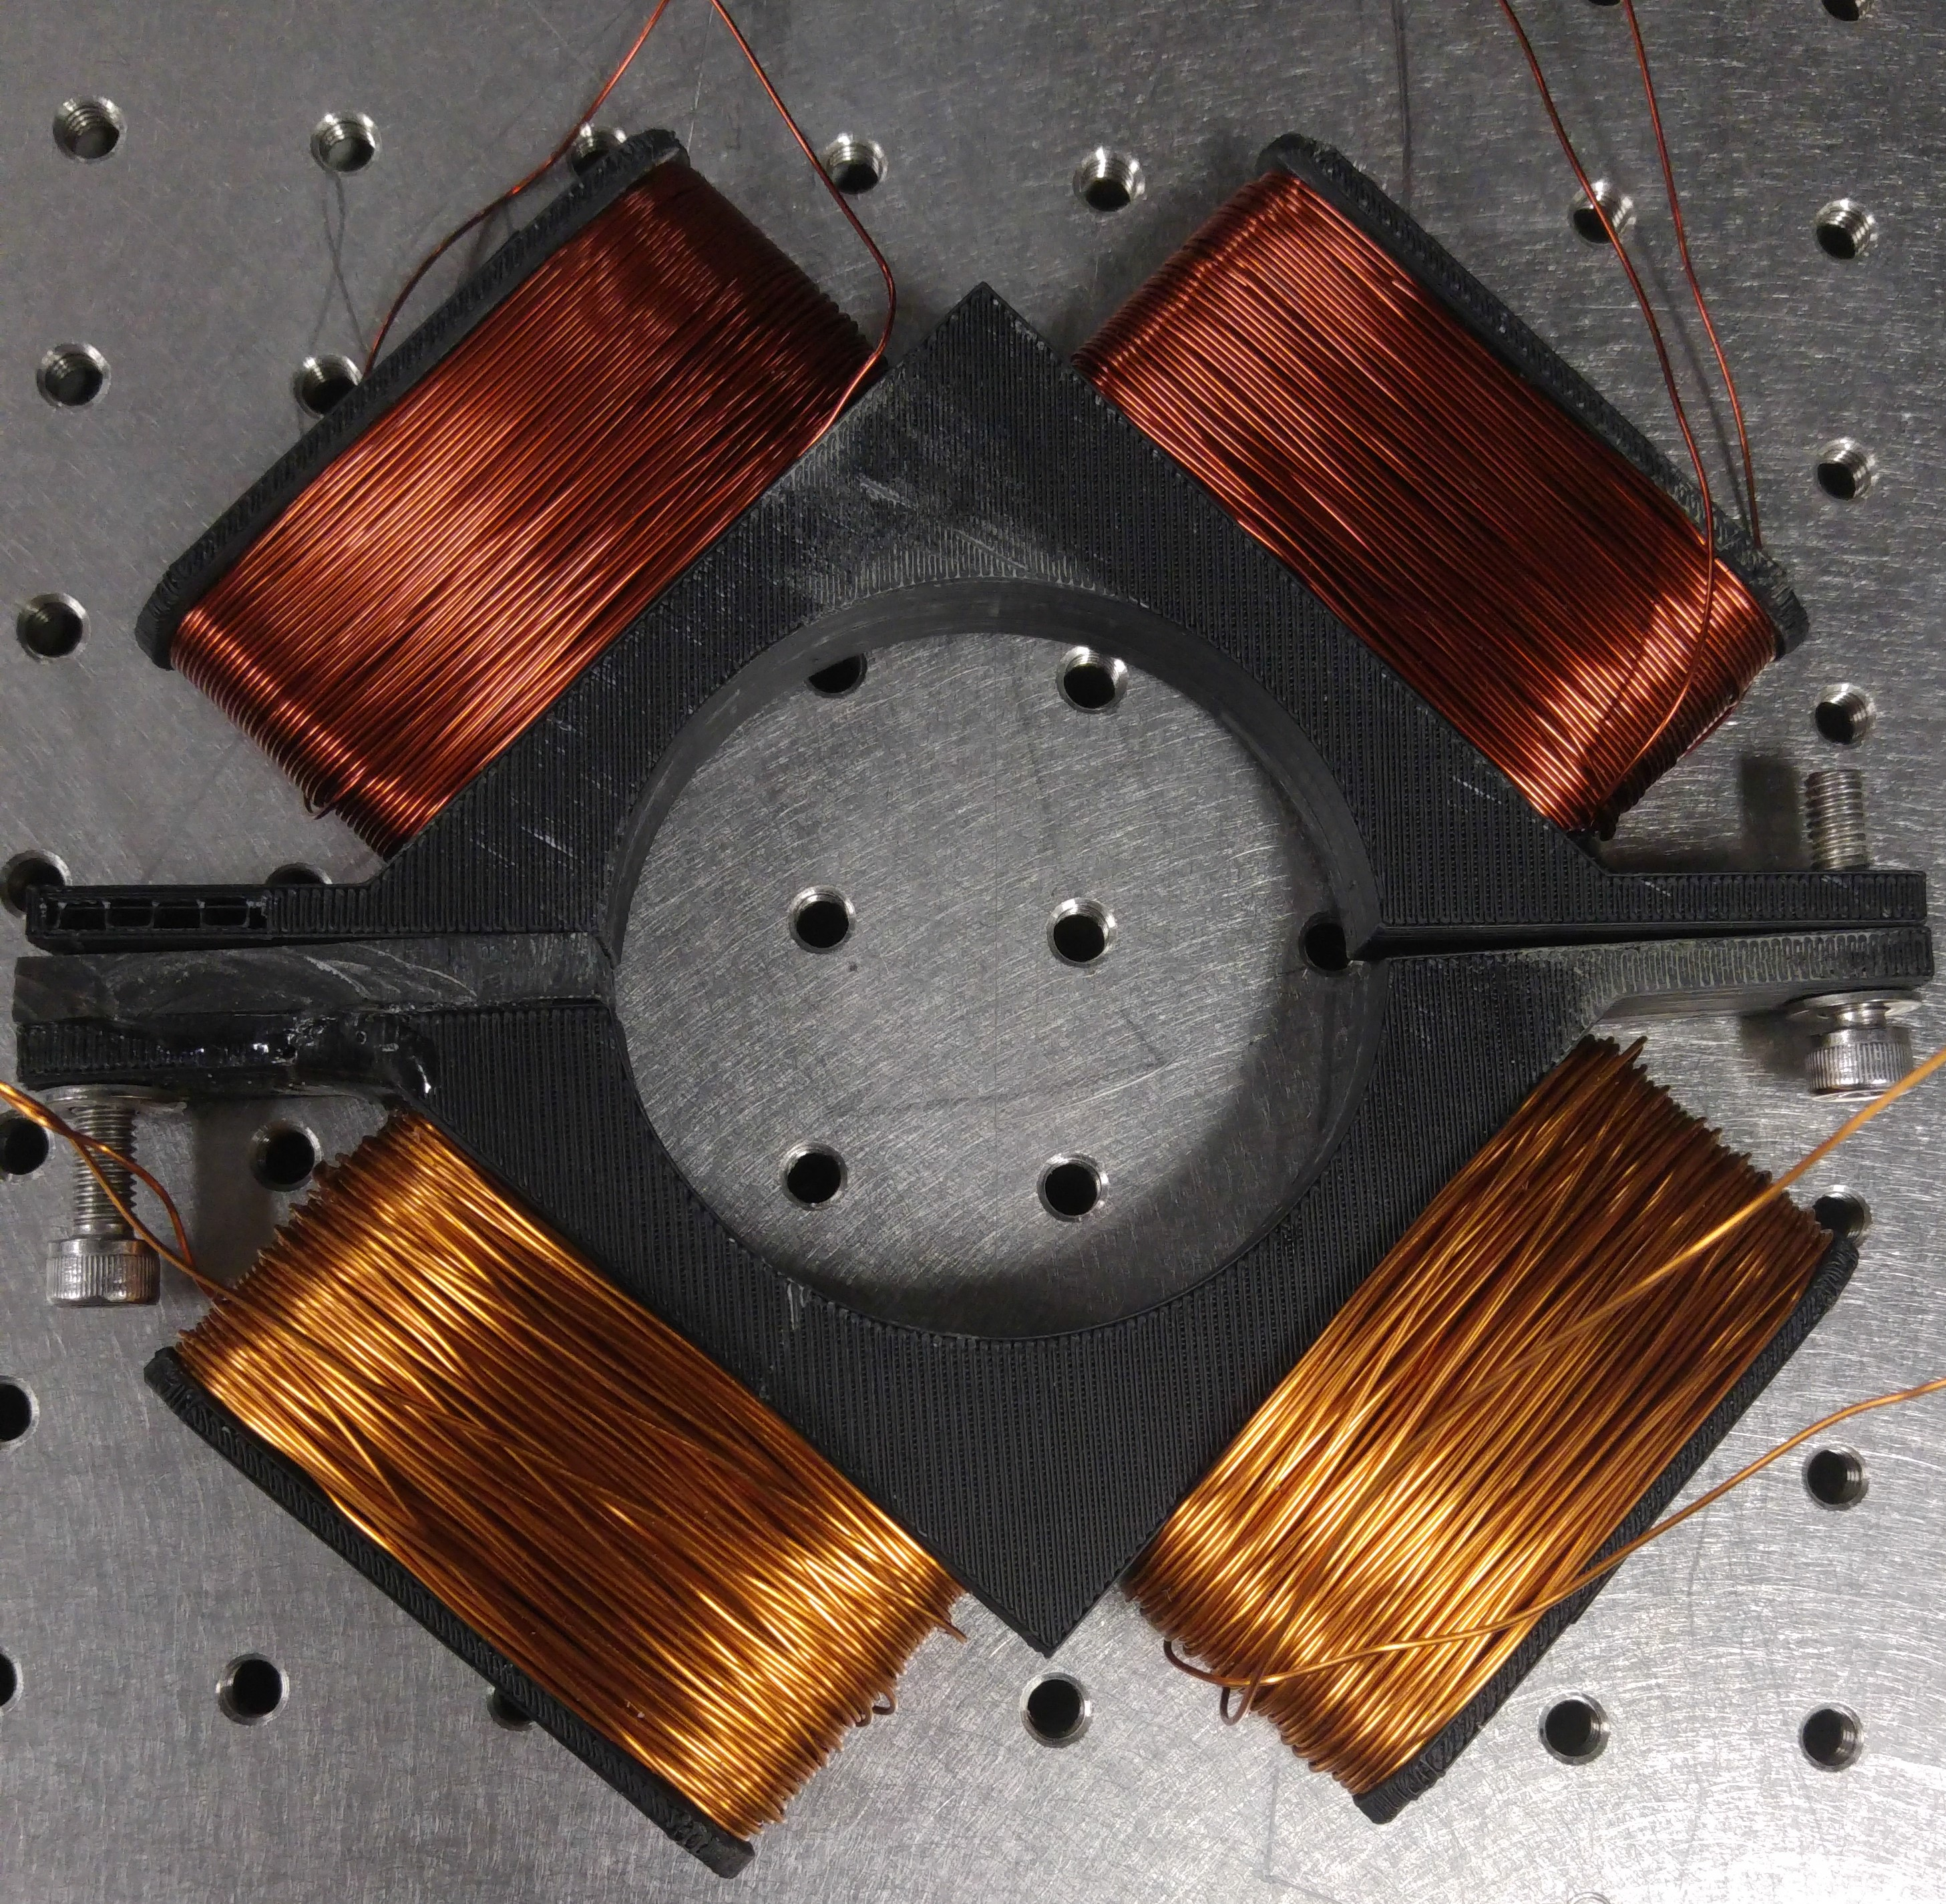
\includegraphics[width=0.5\linewidth]{part2/Figs/quadrupole.jpg}
    \caption[3D printed quadrupole lens.]{The 3D printed chassis wound with copper wire to form a quadrupole lens. The scale is apparent from \unit[70]{mm} inner diameter of the lens and the \unit[25]{mm} spacing of the holes of the optical bench the lens is resting on.}
    \label{figure:quadrupole}
\end{figure}

\subsection{Quadrupole Simulations}

A simple charged particle simulator was created with the ability to propagate charged particles through arbitrary magnetic fields which in this case were formed by a parameterised quadrupole lens.
The code for these simulations is given in Appendix~\ref{appendix:code}.
The electrons used in the simulations had a beam energy of \unit[8.5]{keV} and an initial \gls{rms} beam radius of \unit[5]{mm}, similar to electron bunches produced by the \gls{caes}.
The electrons were given normally distributed randomly determined initial transverse velocities with the $x$ velocity distribution given an \gls{rms} width of \unit[10]{km\,s$^{-1}$} and the $y$ velocity distribution given an \gls{rms} width of \unit[20]{km\,s$^{-1}$} which produced an astigmatism similar to that observed experimentally.
The electrons bunches were propagated \unit[250]{mm} to the virtual quadrupole lens, through the lens, for another \unit[250]{mm} to a focusing lens, and finally for another \unit[500]{mm} to observe the beam foci.
A number of figures of merit were available to determine the ideal design, such as the degree to which the quadrupole lens was able to correct the astigmatism, the current required for the lens to correct for the astigmatism, and the size of the beam waist.

A portion of the simulation results are shown in Figure~\ref{figure:quad_sims} and the main figures of merit used were the separation of the foci for each axis and the number of current turns required to achieve minimum foci separation for a given solenoid transverse radius.
The results indicate that negligible waist separation requires a transverse solenoid radius of at least \unit[35]{mm} and that the larger the transverse radius the lower the required current turns through the solenoids.

\begin{figure}
    \centering
    %% Creator: Matplotlib, PGF backend
%%
%% To include the figure in your LaTeX document, write
%%   \input{<filename>.pgf}
%%
%% Make sure the required packages are loaded in your preamble
%%   \usepackage{pgf}
%%
%% Figures using additional raster images can only be included by \input if
%% they are in the same directory as the main LaTeX file. For loading figures
%% from other directories you can use the `import` package
%%   \usepackage{import}
%% and then include the figures with
%%   \import{<path to file>}{<filename>.pgf}
%%
%% Matplotlib used the following preamble
%%
\begingroup%
\makeatletter%
\begin{pgfpicture}%
\pgfpathrectangle{\pgfpointorigin}{\pgfqpoint{5.710000in}{1.903333in}}%
\pgfusepath{use as bounding box, clip}%
\begin{pgfscope}%
\pgfsetbuttcap%
\pgfsetmiterjoin%
\definecolor{currentfill}{rgb}{1.000000,1.000000,1.000000}%
\pgfsetfillcolor{currentfill}%
\pgfsetlinewidth{0.000000pt}%
\definecolor{currentstroke}{rgb}{1.000000,1.000000,1.000000}%
\pgfsetstrokecolor{currentstroke}%
\pgfsetdash{}{0pt}%
\pgfpathmoveto{\pgfqpoint{0.000000in}{0.000000in}}%
\pgfpathlineto{\pgfqpoint{5.710000in}{0.000000in}}%
\pgfpathlineto{\pgfqpoint{5.710000in}{1.903333in}}%
\pgfpathlineto{\pgfqpoint{0.000000in}{1.903333in}}%
\pgfpathclose%
\pgfusepath{fill}%
\end{pgfscope}%
\begin{pgfscope}%
\pgfsetbuttcap%
\pgfsetmiterjoin%
\definecolor{currentfill}{rgb}{1.000000,1.000000,1.000000}%
\pgfsetfillcolor{currentfill}%
\pgfsetlinewidth{0.000000pt}%
\definecolor{currentstroke}{rgb}{0.000000,0.000000,0.000000}%
\pgfsetstrokecolor{currentstroke}%
\pgfsetstrokeopacity{0.000000}%
\pgfsetdash{}{0pt}%
\pgfpathmoveto{\pgfqpoint{0.536657in}{0.521575in}}%
\pgfpathlineto{\pgfqpoint{2.676222in}{0.521575in}}%
\pgfpathlineto{\pgfqpoint{2.676222in}{1.571809in}}%
\pgfpathlineto{\pgfqpoint{0.536657in}{1.571809in}}%
\pgfpathclose%
\pgfusepath{fill}%
\end{pgfscope}%
\begin{pgfscope}%
\pgfpathrectangle{\pgfqpoint{0.536657in}{0.521575in}}{\pgfqpoint{2.139565in}{1.050235in}} %
\pgfusepath{clip}%
\pgfsetrectcap%
\pgfsetroundjoin%
\pgfsetlinewidth{1.003750pt}%
\definecolor{currentstroke}{rgb}{0.000000,0.000000,1.000000}%
\pgfsetstrokecolor{currentstroke}%
\pgfsetdash{}{0pt}%
\pgfpathmoveto{\pgfqpoint{0.804103in}{1.446243in}}%
\pgfpathlineto{\pgfqpoint{0.927539in}{1.236091in}}%
\pgfpathlineto{\pgfqpoint{1.050976in}{0.983909in}}%
\pgfpathlineto{\pgfqpoint{1.174412in}{0.773757in}}%
\pgfpathlineto{\pgfqpoint{1.297849in}{0.521575in}}%
\pgfpathlineto{\pgfqpoint{1.421285in}{0.521575in}}%
\pgfpathlineto{\pgfqpoint{1.544722in}{0.521575in}}%
\pgfpathlineto{\pgfqpoint{1.668158in}{0.563605in}}%
\pgfpathlineto{\pgfqpoint{1.791595in}{0.542590in}}%
\pgfpathlineto{\pgfqpoint{1.915031in}{0.521575in}}%
\pgfpathlineto{\pgfqpoint{2.038467in}{0.521575in}}%
\pgfpathlineto{\pgfqpoint{2.161904in}{0.521575in}}%
\pgfpathlineto{\pgfqpoint{2.285340in}{0.521575in}}%
\pgfpathlineto{\pgfqpoint{2.408777in}{0.521575in}}%
\pgfusepath{stroke}%
\end{pgfscope}%
\begin{pgfscope}%
\pgfpathrectangle{\pgfqpoint{0.536657in}{0.521575in}}{\pgfqpoint{2.139565in}{1.050235in}} %
\pgfusepath{clip}%
\pgfsetbuttcap%
\pgfsetroundjoin%
\definecolor{currentfill}{rgb}{0.000000,0.000000,1.000000}%
\pgfsetfillcolor{currentfill}%
\pgfsetlinewidth{0.501875pt}%
\definecolor{currentstroke}{rgb}{0.000000,0.000000,1.000000}%
\pgfsetstrokecolor{currentstroke}%
\pgfsetdash{}{0pt}%
\pgfsys@defobject{currentmarker}{\pgfqpoint{-0.041667in}{-0.041667in}}{\pgfqpoint{0.041667in}{0.041667in}}{%
\pgfpathmoveto{\pgfqpoint{-0.041667in}{-0.041667in}}%
\pgfpathlineto{\pgfqpoint{0.041667in}{0.041667in}}%
\pgfpathmoveto{\pgfqpoint{-0.041667in}{0.041667in}}%
\pgfpathlineto{\pgfqpoint{0.041667in}{-0.041667in}}%
\pgfusepath{stroke,fill}%
}%
\begin{pgfscope}%
\pgfsys@transformshift{0.804103in}{1.446243in}%
\pgfsys@useobject{currentmarker}{}%
\end{pgfscope}%
\begin{pgfscope}%
\pgfsys@transformshift{0.927539in}{1.236091in}%
\pgfsys@useobject{currentmarker}{}%
\end{pgfscope}%
\begin{pgfscope}%
\pgfsys@transformshift{1.050976in}{0.983909in}%
\pgfsys@useobject{currentmarker}{}%
\end{pgfscope}%
\begin{pgfscope}%
\pgfsys@transformshift{1.174412in}{0.773757in}%
\pgfsys@useobject{currentmarker}{}%
\end{pgfscope}%
\begin{pgfscope}%
\pgfsys@transformshift{1.297849in}{0.521575in}%
\pgfsys@useobject{currentmarker}{}%
\end{pgfscope}%
\begin{pgfscope}%
\pgfsys@transformshift{1.421285in}{0.521575in}%
\pgfsys@useobject{currentmarker}{}%
\end{pgfscope}%
\begin{pgfscope}%
\pgfsys@transformshift{1.544722in}{0.521575in}%
\pgfsys@useobject{currentmarker}{}%
\end{pgfscope}%
\begin{pgfscope}%
\pgfsys@transformshift{1.668158in}{0.563605in}%
\pgfsys@useobject{currentmarker}{}%
\end{pgfscope}%
\begin{pgfscope}%
\pgfsys@transformshift{1.791595in}{0.542590in}%
\pgfsys@useobject{currentmarker}{}%
\end{pgfscope}%
\begin{pgfscope}%
\pgfsys@transformshift{1.915031in}{0.521575in}%
\pgfsys@useobject{currentmarker}{}%
\end{pgfscope}%
\begin{pgfscope}%
\pgfsys@transformshift{2.038467in}{0.521575in}%
\pgfsys@useobject{currentmarker}{}%
\end{pgfscope}%
\begin{pgfscope}%
\pgfsys@transformshift{2.161904in}{0.521575in}%
\pgfsys@useobject{currentmarker}{}%
\end{pgfscope}%
\begin{pgfscope}%
\pgfsys@transformshift{2.285340in}{0.521575in}%
\pgfsys@useobject{currentmarker}{}%
\end{pgfscope}%
\begin{pgfscope}%
\pgfsys@transformshift{2.408777in}{0.521575in}%
\pgfsys@useobject{currentmarker}{}%
\end{pgfscope}%
\end{pgfscope}%
\begin{pgfscope}%
\pgfsetrectcap%
\pgfsetmiterjoin%
\pgfsetlinewidth{1.003750pt}%
\definecolor{currentstroke}{rgb}{0.000000,0.000000,0.000000}%
\pgfsetstrokecolor{currentstroke}%
\pgfsetdash{}{0pt}%
\pgfpathmoveto{\pgfqpoint{0.536657in}{0.521575in}}%
\pgfpathlineto{\pgfqpoint{0.536657in}{1.571809in}}%
\pgfusepath{stroke}%
\end{pgfscope}%
\begin{pgfscope}%
\pgfsetrectcap%
\pgfsetmiterjoin%
\pgfsetlinewidth{1.003750pt}%
\definecolor{currentstroke}{rgb}{0.000000,0.000000,0.000000}%
\pgfsetstrokecolor{currentstroke}%
\pgfsetdash{}{0pt}%
\pgfpathmoveto{\pgfqpoint{0.536657in}{0.521575in}}%
\pgfpathlineto{\pgfqpoint{2.676222in}{0.521575in}}%
\pgfusepath{stroke}%
\end{pgfscope}%
\begin{pgfscope}%
\pgfsetrectcap%
\pgfsetmiterjoin%
\pgfsetlinewidth{1.003750pt}%
\definecolor{currentstroke}{rgb}{0.000000,0.000000,0.000000}%
\pgfsetstrokecolor{currentstroke}%
\pgfsetdash{}{0pt}%
\pgfpathmoveto{\pgfqpoint{2.676222in}{0.521575in}}%
\pgfpathlineto{\pgfqpoint{2.676222in}{1.571809in}}%
\pgfusepath{stroke}%
\end{pgfscope}%
\begin{pgfscope}%
\pgfsetrectcap%
\pgfsetmiterjoin%
\pgfsetlinewidth{1.003750pt}%
\definecolor{currentstroke}{rgb}{0.000000,0.000000,0.000000}%
\pgfsetstrokecolor{currentstroke}%
\pgfsetdash{}{0pt}%
\pgfpathmoveto{\pgfqpoint{0.536657in}{1.571809in}}%
\pgfpathlineto{\pgfqpoint{2.676222in}{1.571809in}}%
\pgfusepath{stroke}%
\end{pgfscope}%
\begin{pgfscope}%
\pgfsetbuttcap%
\pgfsetroundjoin%
\definecolor{currentfill}{rgb}{0.000000,0.000000,0.000000}%
\pgfsetfillcolor{currentfill}%
\pgfsetlinewidth{0.501875pt}%
\definecolor{currentstroke}{rgb}{0.000000,0.000000,0.000000}%
\pgfsetstrokecolor{currentstroke}%
\pgfsetdash{}{0pt}%
\pgfsys@defobject{currentmarker}{\pgfqpoint{0.000000in}{0.000000in}}{\pgfqpoint{0.000000in}{0.055556in}}{%
\pgfpathmoveto{\pgfqpoint{0.000000in}{0.000000in}}%
\pgfpathlineto{\pgfqpoint{0.000000in}{0.055556in}}%
\pgfusepath{stroke,fill}%
}%
\begin{pgfscope}%
\pgfsys@transformshift{0.536657in}{0.521575in}%
\pgfsys@useobject{currentmarker}{}%
\end{pgfscope}%
\end{pgfscope}%
\begin{pgfscope}%
\pgfsetbuttcap%
\pgfsetroundjoin%
\definecolor{currentfill}{rgb}{0.000000,0.000000,0.000000}%
\pgfsetfillcolor{currentfill}%
\pgfsetlinewidth{0.501875pt}%
\definecolor{currentstroke}{rgb}{0.000000,0.000000,0.000000}%
\pgfsetstrokecolor{currentstroke}%
\pgfsetdash{}{0pt}%
\pgfsys@defobject{currentmarker}{\pgfqpoint{0.000000in}{-0.055556in}}{\pgfqpoint{0.000000in}{0.000000in}}{%
\pgfpathmoveto{\pgfqpoint{0.000000in}{0.000000in}}%
\pgfpathlineto{\pgfqpoint{0.000000in}{-0.055556in}}%
\pgfusepath{stroke,fill}%
}%
\begin{pgfscope}%
\pgfsys@transformshift{0.536657in}{1.571809in}%
\pgfsys@useobject{currentmarker}{}%
\end{pgfscope}%
\end{pgfscope}%
\begin{pgfscope}%
\pgftext[x=0.536657in,y=0.466019in,,top]{\fontsize{10.000000}{12.000000}\selectfont \(\displaystyle 0\)}%
\end{pgfscope}%
\begin{pgfscope}%
\pgfsetbuttcap%
\pgfsetroundjoin%
\definecolor{currentfill}{rgb}{0.000000,0.000000,0.000000}%
\pgfsetfillcolor{currentfill}%
\pgfsetlinewidth{0.501875pt}%
\definecolor{currentstroke}{rgb}{0.000000,0.000000,0.000000}%
\pgfsetstrokecolor{currentstroke}%
\pgfsetdash{}{0pt}%
\pgfsys@defobject{currentmarker}{\pgfqpoint{0.000000in}{0.000000in}}{\pgfqpoint{0.000000in}{0.055556in}}{%
\pgfpathmoveto{\pgfqpoint{0.000000in}{0.000000in}}%
\pgfpathlineto{\pgfqpoint{0.000000in}{0.055556in}}%
\pgfusepath{stroke,fill}%
}%
\begin{pgfscope}%
\pgfsys@transformshift{0.893252in}{0.521575in}%
\pgfsys@useobject{currentmarker}{}%
\end{pgfscope}%
\end{pgfscope}%
\begin{pgfscope}%
\pgfsetbuttcap%
\pgfsetroundjoin%
\definecolor{currentfill}{rgb}{0.000000,0.000000,0.000000}%
\pgfsetfillcolor{currentfill}%
\pgfsetlinewidth{0.501875pt}%
\definecolor{currentstroke}{rgb}{0.000000,0.000000,0.000000}%
\pgfsetstrokecolor{currentstroke}%
\pgfsetdash{}{0pt}%
\pgfsys@defobject{currentmarker}{\pgfqpoint{0.000000in}{-0.055556in}}{\pgfqpoint{0.000000in}{0.000000in}}{%
\pgfpathmoveto{\pgfqpoint{0.000000in}{0.000000in}}%
\pgfpathlineto{\pgfqpoint{0.000000in}{-0.055556in}}%
\pgfusepath{stroke,fill}%
}%
\begin{pgfscope}%
\pgfsys@transformshift{0.893252in}{1.571809in}%
\pgfsys@useobject{currentmarker}{}%
\end{pgfscope}%
\end{pgfscope}%
\begin{pgfscope}%
\pgftext[x=0.893252in,y=0.466019in,,top]{\fontsize{10.000000}{12.000000}\selectfont \(\displaystyle 20\)}%
\end{pgfscope}%
\begin{pgfscope}%
\pgfsetbuttcap%
\pgfsetroundjoin%
\definecolor{currentfill}{rgb}{0.000000,0.000000,0.000000}%
\pgfsetfillcolor{currentfill}%
\pgfsetlinewidth{0.501875pt}%
\definecolor{currentstroke}{rgb}{0.000000,0.000000,0.000000}%
\pgfsetstrokecolor{currentstroke}%
\pgfsetdash{}{0pt}%
\pgfsys@defobject{currentmarker}{\pgfqpoint{0.000000in}{0.000000in}}{\pgfqpoint{0.000000in}{0.055556in}}{%
\pgfpathmoveto{\pgfqpoint{0.000000in}{0.000000in}}%
\pgfpathlineto{\pgfqpoint{0.000000in}{0.055556in}}%
\pgfusepath{stroke,fill}%
}%
\begin{pgfscope}%
\pgfsys@transformshift{1.249846in}{0.521575in}%
\pgfsys@useobject{currentmarker}{}%
\end{pgfscope}%
\end{pgfscope}%
\begin{pgfscope}%
\pgfsetbuttcap%
\pgfsetroundjoin%
\definecolor{currentfill}{rgb}{0.000000,0.000000,0.000000}%
\pgfsetfillcolor{currentfill}%
\pgfsetlinewidth{0.501875pt}%
\definecolor{currentstroke}{rgb}{0.000000,0.000000,0.000000}%
\pgfsetstrokecolor{currentstroke}%
\pgfsetdash{}{0pt}%
\pgfsys@defobject{currentmarker}{\pgfqpoint{0.000000in}{-0.055556in}}{\pgfqpoint{0.000000in}{0.000000in}}{%
\pgfpathmoveto{\pgfqpoint{0.000000in}{0.000000in}}%
\pgfpathlineto{\pgfqpoint{0.000000in}{-0.055556in}}%
\pgfusepath{stroke,fill}%
}%
\begin{pgfscope}%
\pgfsys@transformshift{1.249846in}{1.571809in}%
\pgfsys@useobject{currentmarker}{}%
\end{pgfscope}%
\end{pgfscope}%
\begin{pgfscope}%
\pgftext[x=1.249846in,y=0.466019in,,top]{\fontsize{10.000000}{12.000000}\selectfont \(\displaystyle 40\)}%
\end{pgfscope}%
\begin{pgfscope}%
\pgfsetbuttcap%
\pgfsetroundjoin%
\definecolor{currentfill}{rgb}{0.000000,0.000000,0.000000}%
\pgfsetfillcolor{currentfill}%
\pgfsetlinewidth{0.501875pt}%
\definecolor{currentstroke}{rgb}{0.000000,0.000000,0.000000}%
\pgfsetstrokecolor{currentstroke}%
\pgfsetdash{}{0pt}%
\pgfsys@defobject{currentmarker}{\pgfqpoint{0.000000in}{0.000000in}}{\pgfqpoint{0.000000in}{0.055556in}}{%
\pgfpathmoveto{\pgfqpoint{0.000000in}{0.000000in}}%
\pgfpathlineto{\pgfqpoint{0.000000in}{0.055556in}}%
\pgfusepath{stroke,fill}%
}%
\begin{pgfscope}%
\pgfsys@transformshift{1.606440in}{0.521575in}%
\pgfsys@useobject{currentmarker}{}%
\end{pgfscope}%
\end{pgfscope}%
\begin{pgfscope}%
\pgfsetbuttcap%
\pgfsetroundjoin%
\definecolor{currentfill}{rgb}{0.000000,0.000000,0.000000}%
\pgfsetfillcolor{currentfill}%
\pgfsetlinewidth{0.501875pt}%
\definecolor{currentstroke}{rgb}{0.000000,0.000000,0.000000}%
\pgfsetstrokecolor{currentstroke}%
\pgfsetdash{}{0pt}%
\pgfsys@defobject{currentmarker}{\pgfqpoint{0.000000in}{-0.055556in}}{\pgfqpoint{0.000000in}{0.000000in}}{%
\pgfpathmoveto{\pgfqpoint{0.000000in}{0.000000in}}%
\pgfpathlineto{\pgfqpoint{0.000000in}{-0.055556in}}%
\pgfusepath{stroke,fill}%
}%
\begin{pgfscope}%
\pgfsys@transformshift{1.606440in}{1.571809in}%
\pgfsys@useobject{currentmarker}{}%
\end{pgfscope}%
\end{pgfscope}%
\begin{pgfscope}%
\pgftext[x=1.606440in,y=0.466019in,,top]{\fontsize{10.000000}{12.000000}\selectfont \(\displaystyle 60\)}%
\end{pgfscope}%
\begin{pgfscope}%
\pgfsetbuttcap%
\pgfsetroundjoin%
\definecolor{currentfill}{rgb}{0.000000,0.000000,0.000000}%
\pgfsetfillcolor{currentfill}%
\pgfsetlinewidth{0.501875pt}%
\definecolor{currentstroke}{rgb}{0.000000,0.000000,0.000000}%
\pgfsetstrokecolor{currentstroke}%
\pgfsetdash{}{0pt}%
\pgfsys@defobject{currentmarker}{\pgfqpoint{0.000000in}{0.000000in}}{\pgfqpoint{0.000000in}{0.055556in}}{%
\pgfpathmoveto{\pgfqpoint{0.000000in}{0.000000in}}%
\pgfpathlineto{\pgfqpoint{0.000000in}{0.055556in}}%
\pgfusepath{stroke,fill}%
}%
\begin{pgfscope}%
\pgfsys@transformshift{1.963034in}{0.521575in}%
\pgfsys@useobject{currentmarker}{}%
\end{pgfscope}%
\end{pgfscope}%
\begin{pgfscope}%
\pgfsetbuttcap%
\pgfsetroundjoin%
\definecolor{currentfill}{rgb}{0.000000,0.000000,0.000000}%
\pgfsetfillcolor{currentfill}%
\pgfsetlinewidth{0.501875pt}%
\definecolor{currentstroke}{rgb}{0.000000,0.000000,0.000000}%
\pgfsetstrokecolor{currentstroke}%
\pgfsetdash{}{0pt}%
\pgfsys@defobject{currentmarker}{\pgfqpoint{0.000000in}{-0.055556in}}{\pgfqpoint{0.000000in}{0.000000in}}{%
\pgfpathmoveto{\pgfqpoint{0.000000in}{0.000000in}}%
\pgfpathlineto{\pgfqpoint{0.000000in}{-0.055556in}}%
\pgfusepath{stroke,fill}%
}%
\begin{pgfscope}%
\pgfsys@transformshift{1.963034in}{1.571809in}%
\pgfsys@useobject{currentmarker}{}%
\end{pgfscope}%
\end{pgfscope}%
\begin{pgfscope}%
\pgftext[x=1.963034in,y=0.466019in,,top]{\fontsize{10.000000}{12.000000}\selectfont \(\displaystyle 80\)}%
\end{pgfscope}%
\begin{pgfscope}%
\pgfsetbuttcap%
\pgfsetroundjoin%
\definecolor{currentfill}{rgb}{0.000000,0.000000,0.000000}%
\pgfsetfillcolor{currentfill}%
\pgfsetlinewidth{0.501875pt}%
\definecolor{currentstroke}{rgb}{0.000000,0.000000,0.000000}%
\pgfsetstrokecolor{currentstroke}%
\pgfsetdash{}{0pt}%
\pgfsys@defobject{currentmarker}{\pgfqpoint{0.000000in}{0.000000in}}{\pgfqpoint{0.000000in}{0.055556in}}{%
\pgfpathmoveto{\pgfqpoint{0.000000in}{0.000000in}}%
\pgfpathlineto{\pgfqpoint{0.000000in}{0.055556in}}%
\pgfusepath{stroke,fill}%
}%
\begin{pgfscope}%
\pgfsys@transformshift{2.319628in}{0.521575in}%
\pgfsys@useobject{currentmarker}{}%
\end{pgfscope}%
\end{pgfscope}%
\begin{pgfscope}%
\pgfsetbuttcap%
\pgfsetroundjoin%
\definecolor{currentfill}{rgb}{0.000000,0.000000,0.000000}%
\pgfsetfillcolor{currentfill}%
\pgfsetlinewidth{0.501875pt}%
\definecolor{currentstroke}{rgb}{0.000000,0.000000,0.000000}%
\pgfsetstrokecolor{currentstroke}%
\pgfsetdash{}{0pt}%
\pgfsys@defobject{currentmarker}{\pgfqpoint{0.000000in}{-0.055556in}}{\pgfqpoint{0.000000in}{0.000000in}}{%
\pgfpathmoveto{\pgfqpoint{0.000000in}{0.000000in}}%
\pgfpathlineto{\pgfqpoint{0.000000in}{-0.055556in}}%
\pgfusepath{stroke,fill}%
}%
\begin{pgfscope}%
\pgfsys@transformshift{2.319628in}{1.571809in}%
\pgfsys@useobject{currentmarker}{}%
\end{pgfscope}%
\end{pgfscope}%
\begin{pgfscope}%
\pgftext[x=2.319628in,y=0.466019in,,top]{\fontsize{10.000000}{12.000000}\selectfont \(\displaystyle 100\)}%
\end{pgfscope}%
\begin{pgfscope}%
\pgfsetbuttcap%
\pgfsetroundjoin%
\definecolor{currentfill}{rgb}{0.000000,0.000000,0.000000}%
\pgfsetfillcolor{currentfill}%
\pgfsetlinewidth{0.501875pt}%
\definecolor{currentstroke}{rgb}{0.000000,0.000000,0.000000}%
\pgfsetstrokecolor{currentstroke}%
\pgfsetdash{}{0pt}%
\pgfsys@defobject{currentmarker}{\pgfqpoint{0.000000in}{0.000000in}}{\pgfqpoint{0.000000in}{0.055556in}}{%
\pgfpathmoveto{\pgfqpoint{0.000000in}{0.000000in}}%
\pgfpathlineto{\pgfqpoint{0.000000in}{0.055556in}}%
\pgfusepath{stroke,fill}%
}%
\begin{pgfscope}%
\pgfsys@transformshift{2.676222in}{0.521575in}%
\pgfsys@useobject{currentmarker}{}%
\end{pgfscope}%
\end{pgfscope}%
\begin{pgfscope}%
\pgfsetbuttcap%
\pgfsetroundjoin%
\definecolor{currentfill}{rgb}{0.000000,0.000000,0.000000}%
\pgfsetfillcolor{currentfill}%
\pgfsetlinewidth{0.501875pt}%
\definecolor{currentstroke}{rgb}{0.000000,0.000000,0.000000}%
\pgfsetstrokecolor{currentstroke}%
\pgfsetdash{}{0pt}%
\pgfsys@defobject{currentmarker}{\pgfqpoint{0.000000in}{-0.055556in}}{\pgfqpoint{0.000000in}{0.000000in}}{%
\pgfpathmoveto{\pgfqpoint{0.000000in}{0.000000in}}%
\pgfpathlineto{\pgfqpoint{0.000000in}{-0.055556in}}%
\pgfusepath{stroke,fill}%
}%
\begin{pgfscope}%
\pgfsys@transformshift{2.676222in}{1.571809in}%
\pgfsys@useobject{currentmarker}{}%
\end{pgfscope}%
\end{pgfscope}%
\begin{pgfscope}%
\pgftext[x=2.676222in,y=0.466019in,,top]{\fontsize{10.000000}{12.000000}\selectfont \(\displaystyle 120\)}%
\end{pgfscope}%
\begin{pgfscope}%
\pgftext[x=1.606440in,y=0.273118in,,top]{\fontsize{10.000000}{12.000000}\selectfont Solenoid Transverse Width (mm)}%
\end{pgfscope}%
\begin{pgfscope}%
\pgfsetbuttcap%
\pgfsetroundjoin%
\definecolor{currentfill}{rgb}{0.000000,0.000000,0.000000}%
\pgfsetfillcolor{currentfill}%
\pgfsetlinewidth{0.501875pt}%
\definecolor{currentstroke}{rgb}{0.000000,0.000000,0.000000}%
\pgfsetstrokecolor{currentstroke}%
\pgfsetdash{}{0pt}%
\pgfsys@defobject{currentmarker}{\pgfqpoint{0.000000in}{0.000000in}}{\pgfqpoint{0.055556in}{0.000000in}}{%
\pgfpathmoveto{\pgfqpoint{0.000000in}{0.000000in}}%
\pgfpathlineto{\pgfqpoint{0.055556in}{0.000000in}}%
\pgfusepath{stroke,fill}%
}%
\begin{pgfscope}%
\pgfsys@transformshift{0.536657in}{0.521575in}%
\pgfsys@useobject{currentmarker}{}%
\end{pgfscope}%
\end{pgfscope}%
\begin{pgfscope}%
\pgfsetbuttcap%
\pgfsetroundjoin%
\definecolor{currentfill}{rgb}{0.000000,0.000000,0.000000}%
\pgfsetfillcolor{currentfill}%
\pgfsetlinewidth{0.501875pt}%
\definecolor{currentstroke}{rgb}{0.000000,0.000000,0.000000}%
\pgfsetstrokecolor{currentstroke}%
\pgfsetdash{}{0pt}%
\pgfsys@defobject{currentmarker}{\pgfqpoint{-0.055556in}{0.000000in}}{\pgfqpoint{0.000000in}{0.000000in}}{%
\pgfpathmoveto{\pgfqpoint{0.000000in}{0.000000in}}%
\pgfpathlineto{\pgfqpoint{-0.055556in}{0.000000in}}%
\pgfusepath{stroke,fill}%
}%
\begin{pgfscope}%
\pgfsys@transformshift{2.676222in}{0.521575in}%
\pgfsys@useobject{currentmarker}{}%
\end{pgfscope}%
\end{pgfscope}%
\begin{pgfscope}%
\pgftext[x=0.481102in,y=0.521575in,right,]{\fontsize{10.000000}{12.000000}\selectfont \(\displaystyle 0\)}%
\end{pgfscope}%
\begin{pgfscope}%
\pgfsetbuttcap%
\pgfsetroundjoin%
\definecolor{currentfill}{rgb}{0.000000,0.000000,0.000000}%
\pgfsetfillcolor{currentfill}%
\pgfsetlinewidth{0.501875pt}%
\definecolor{currentstroke}{rgb}{0.000000,0.000000,0.000000}%
\pgfsetstrokecolor{currentstroke}%
\pgfsetdash{}{0pt}%
\pgfsys@defobject{currentmarker}{\pgfqpoint{0.000000in}{0.000000in}}{\pgfqpoint{0.055556in}{0.000000in}}{%
\pgfpathmoveto{\pgfqpoint{0.000000in}{0.000000in}}%
\pgfpathlineto{\pgfqpoint{0.055556in}{0.000000in}}%
\pgfusepath{stroke,fill}%
}%
\begin{pgfscope}%
\pgfsys@transformshift{0.536657in}{0.731622in}%
\pgfsys@useobject{currentmarker}{}%
\end{pgfscope}%
\end{pgfscope}%
\begin{pgfscope}%
\pgfsetbuttcap%
\pgfsetroundjoin%
\definecolor{currentfill}{rgb}{0.000000,0.000000,0.000000}%
\pgfsetfillcolor{currentfill}%
\pgfsetlinewidth{0.501875pt}%
\definecolor{currentstroke}{rgb}{0.000000,0.000000,0.000000}%
\pgfsetstrokecolor{currentstroke}%
\pgfsetdash{}{0pt}%
\pgfsys@defobject{currentmarker}{\pgfqpoint{-0.055556in}{0.000000in}}{\pgfqpoint{0.000000in}{0.000000in}}{%
\pgfpathmoveto{\pgfqpoint{0.000000in}{0.000000in}}%
\pgfpathlineto{\pgfqpoint{-0.055556in}{0.000000in}}%
\pgfusepath{stroke,fill}%
}%
\begin{pgfscope}%
\pgfsys@transformshift{2.676222in}{0.731622in}%
\pgfsys@useobject{currentmarker}{}%
\end{pgfscope}%
\end{pgfscope}%
\begin{pgfscope}%
\pgftext[x=0.481102in,y=0.731622in,right,]{\fontsize{10.000000}{12.000000}\selectfont \(\displaystyle 5\)}%
\end{pgfscope}%
\begin{pgfscope}%
\pgfsetbuttcap%
\pgfsetroundjoin%
\definecolor{currentfill}{rgb}{0.000000,0.000000,0.000000}%
\pgfsetfillcolor{currentfill}%
\pgfsetlinewidth{0.501875pt}%
\definecolor{currentstroke}{rgb}{0.000000,0.000000,0.000000}%
\pgfsetstrokecolor{currentstroke}%
\pgfsetdash{}{0pt}%
\pgfsys@defobject{currentmarker}{\pgfqpoint{0.000000in}{0.000000in}}{\pgfqpoint{0.055556in}{0.000000in}}{%
\pgfpathmoveto{\pgfqpoint{0.000000in}{0.000000in}}%
\pgfpathlineto{\pgfqpoint{0.055556in}{0.000000in}}%
\pgfusepath{stroke,fill}%
}%
\begin{pgfscope}%
\pgfsys@transformshift{0.536657in}{0.941668in}%
\pgfsys@useobject{currentmarker}{}%
\end{pgfscope}%
\end{pgfscope}%
\begin{pgfscope}%
\pgfsetbuttcap%
\pgfsetroundjoin%
\definecolor{currentfill}{rgb}{0.000000,0.000000,0.000000}%
\pgfsetfillcolor{currentfill}%
\pgfsetlinewidth{0.501875pt}%
\definecolor{currentstroke}{rgb}{0.000000,0.000000,0.000000}%
\pgfsetstrokecolor{currentstroke}%
\pgfsetdash{}{0pt}%
\pgfsys@defobject{currentmarker}{\pgfqpoint{-0.055556in}{0.000000in}}{\pgfqpoint{0.000000in}{0.000000in}}{%
\pgfpathmoveto{\pgfqpoint{0.000000in}{0.000000in}}%
\pgfpathlineto{\pgfqpoint{-0.055556in}{0.000000in}}%
\pgfusepath{stroke,fill}%
}%
\begin{pgfscope}%
\pgfsys@transformshift{2.676222in}{0.941668in}%
\pgfsys@useobject{currentmarker}{}%
\end{pgfscope}%
\end{pgfscope}%
\begin{pgfscope}%
\pgftext[x=0.481102in,y=0.941668in,right,]{\fontsize{10.000000}{12.000000}\selectfont \(\displaystyle 10\)}%
\end{pgfscope}%
\begin{pgfscope}%
\pgfsetbuttcap%
\pgfsetroundjoin%
\definecolor{currentfill}{rgb}{0.000000,0.000000,0.000000}%
\pgfsetfillcolor{currentfill}%
\pgfsetlinewidth{0.501875pt}%
\definecolor{currentstroke}{rgb}{0.000000,0.000000,0.000000}%
\pgfsetstrokecolor{currentstroke}%
\pgfsetdash{}{0pt}%
\pgfsys@defobject{currentmarker}{\pgfqpoint{0.000000in}{0.000000in}}{\pgfqpoint{0.055556in}{0.000000in}}{%
\pgfpathmoveto{\pgfqpoint{0.000000in}{0.000000in}}%
\pgfpathlineto{\pgfqpoint{0.055556in}{0.000000in}}%
\pgfusepath{stroke,fill}%
}%
\begin{pgfscope}%
\pgfsys@transformshift{0.536657in}{1.151715in}%
\pgfsys@useobject{currentmarker}{}%
\end{pgfscope}%
\end{pgfscope}%
\begin{pgfscope}%
\pgfsetbuttcap%
\pgfsetroundjoin%
\definecolor{currentfill}{rgb}{0.000000,0.000000,0.000000}%
\pgfsetfillcolor{currentfill}%
\pgfsetlinewidth{0.501875pt}%
\definecolor{currentstroke}{rgb}{0.000000,0.000000,0.000000}%
\pgfsetstrokecolor{currentstroke}%
\pgfsetdash{}{0pt}%
\pgfsys@defobject{currentmarker}{\pgfqpoint{-0.055556in}{0.000000in}}{\pgfqpoint{0.000000in}{0.000000in}}{%
\pgfpathmoveto{\pgfqpoint{0.000000in}{0.000000in}}%
\pgfpathlineto{\pgfqpoint{-0.055556in}{0.000000in}}%
\pgfusepath{stroke,fill}%
}%
\begin{pgfscope}%
\pgfsys@transformshift{2.676222in}{1.151715in}%
\pgfsys@useobject{currentmarker}{}%
\end{pgfscope}%
\end{pgfscope}%
\begin{pgfscope}%
\pgftext[x=0.481102in,y=1.151715in,right,]{\fontsize{10.000000}{12.000000}\selectfont \(\displaystyle 15\)}%
\end{pgfscope}%
\begin{pgfscope}%
\pgfsetbuttcap%
\pgfsetroundjoin%
\definecolor{currentfill}{rgb}{0.000000,0.000000,0.000000}%
\pgfsetfillcolor{currentfill}%
\pgfsetlinewidth{0.501875pt}%
\definecolor{currentstroke}{rgb}{0.000000,0.000000,0.000000}%
\pgfsetstrokecolor{currentstroke}%
\pgfsetdash{}{0pt}%
\pgfsys@defobject{currentmarker}{\pgfqpoint{0.000000in}{0.000000in}}{\pgfqpoint{0.055556in}{0.000000in}}{%
\pgfpathmoveto{\pgfqpoint{0.000000in}{0.000000in}}%
\pgfpathlineto{\pgfqpoint{0.055556in}{0.000000in}}%
\pgfusepath{stroke,fill}%
}%
\begin{pgfscope}%
\pgfsys@transformshift{0.536657in}{1.361762in}%
\pgfsys@useobject{currentmarker}{}%
\end{pgfscope}%
\end{pgfscope}%
\begin{pgfscope}%
\pgfsetbuttcap%
\pgfsetroundjoin%
\definecolor{currentfill}{rgb}{0.000000,0.000000,0.000000}%
\pgfsetfillcolor{currentfill}%
\pgfsetlinewidth{0.501875pt}%
\definecolor{currentstroke}{rgb}{0.000000,0.000000,0.000000}%
\pgfsetstrokecolor{currentstroke}%
\pgfsetdash{}{0pt}%
\pgfsys@defobject{currentmarker}{\pgfqpoint{-0.055556in}{0.000000in}}{\pgfqpoint{0.000000in}{0.000000in}}{%
\pgfpathmoveto{\pgfqpoint{0.000000in}{0.000000in}}%
\pgfpathlineto{\pgfqpoint{-0.055556in}{0.000000in}}%
\pgfusepath{stroke,fill}%
}%
\begin{pgfscope}%
\pgfsys@transformshift{2.676222in}{1.361762in}%
\pgfsys@useobject{currentmarker}{}%
\end{pgfscope}%
\end{pgfscope}%
\begin{pgfscope}%
\pgftext[x=0.481102in,y=1.361762in,right,]{\fontsize{10.000000}{12.000000}\selectfont \(\displaystyle 20\)}%
\end{pgfscope}%
\begin{pgfscope}%
\pgfsetbuttcap%
\pgfsetroundjoin%
\definecolor{currentfill}{rgb}{0.000000,0.000000,0.000000}%
\pgfsetfillcolor{currentfill}%
\pgfsetlinewidth{0.501875pt}%
\definecolor{currentstroke}{rgb}{0.000000,0.000000,0.000000}%
\pgfsetstrokecolor{currentstroke}%
\pgfsetdash{}{0pt}%
\pgfsys@defobject{currentmarker}{\pgfqpoint{0.000000in}{0.000000in}}{\pgfqpoint{0.055556in}{0.000000in}}{%
\pgfpathmoveto{\pgfqpoint{0.000000in}{0.000000in}}%
\pgfpathlineto{\pgfqpoint{0.055556in}{0.000000in}}%
\pgfusepath{stroke,fill}%
}%
\begin{pgfscope}%
\pgfsys@transformshift{0.536657in}{1.571809in}%
\pgfsys@useobject{currentmarker}{}%
\end{pgfscope}%
\end{pgfscope}%
\begin{pgfscope}%
\pgfsetbuttcap%
\pgfsetroundjoin%
\definecolor{currentfill}{rgb}{0.000000,0.000000,0.000000}%
\pgfsetfillcolor{currentfill}%
\pgfsetlinewidth{0.501875pt}%
\definecolor{currentstroke}{rgb}{0.000000,0.000000,0.000000}%
\pgfsetstrokecolor{currentstroke}%
\pgfsetdash{}{0pt}%
\pgfsys@defobject{currentmarker}{\pgfqpoint{-0.055556in}{0.000000in}}{\pgfqpoint{0.000000in}{0.000000in}}{%
\pgfpathmoveto{\pgfqpoint{0.000000in}{0.000000in}}%
\pgfpathlineto{\pgfqpoint{-0.055556in}{0.000000in}}%
\pgfusepath{stroke,fill}%
}%
\begin{pgfscope}%
\pgfsys@transformshift{2.676222in}{1.571809in}%
\pgfsys@useobject{currentmarker}{}%
\end{pgfscope}%
\end{pgfscope}%
\begin{pgfscope}%
\pgftext[x=0.481102in,y=1.571809in,right,]{\fontsize{10.000000}{12.000000}\selectfont \(\displaystyle 25\)}%
\end{pgfscope}%
\begin{pgfscope}%
\pgftext[x=0.272768in,y=1.046692in,,bottom,rotate=90.000000]{\fontsize{10.000000}{12.000000}\selectfont Waist Separation (mm)}%
\end{pgfscope}%
\begin{pgfscope}%
\pgftext[x=1.606440in,y=1.641254in,,base]{\fontsize{12.000000}{14.400000}\selectfont Waist Separation}%
\end{pgfscope}%
\begin{pgfscope}%
\pgfsetbuttcap%
\pgfsetmiterjoin%
\definecolor{currentfill}{rgb}{1.000000,1.000000,1.000000}%
\pgfsetfillcolor{currentfill}%
\pgfsetlinewidth{0.000000pt}%
\definecolor{currentstroke}{rgb}{0.000000,0.000000,0.000000}%
\pgfsetstrokecolor{currentstroke}%
\pgfsetstrokeopacity{0.000000}%
\pgfsetdash{}{0pt}%
\pgfpathmoveto{\pgfqpoint{3.316657in}{0.521575in}}%
\pgfpathlineto{\pgfqpoint{5.456222in}{0.521575in}}%
\pgfpathlineto{\pgfqpoint{5.456222in}{1.571809in}}%
\pgfpathlineto{\pgfqpoint{3.316657in}{1.571809in}}%
\pgfpathclose%
\pgfusepath{fill}%
\end{pgfscope}%
\begin{pgfscope}%
\pgfpathrectangle{\pgfqpoint{3.316657in}{0.521575in}}{\pgfqpoint{2.139565in}{1.050235in}} %
\pgfusepath{clip}%
\pgfsetrectcap%
\pgfsetroundjoin%
\pgfsetlinewidth{1.003750pt}%
\definecolor{currentstroke}{rgb}{0.000000,0.000000,1.000000}%
\pgfsetstrokecolor{currentstroke}%
\pgfsetdash{}{0pt}%
\pgfpathmoveto{\pgfqpoint{3.584103in}{1.513463in}}%
\pgfpathlineto{\pgfqpoint{3.707539in}{1.455117in}}%
\pgfpathlineto{\pgfqpoint{3.830976in}{1.513463in}}%
\pgfpathlineto{\pgfqpoint{3.954412in}{1.513463in}}%
\pgfpathlineto{\pgfqpoint{4.077849in}{1.513463in}}%
\pgfpathlineto{\pgfqpoint{4.201285in}{1.280077in}}%
\pgfpathlineto{\pgfqpoint{4.324722in}{1.105038in}}%
\pgfpathlineto{\pgfqpoint{4.448158in}{0.929999in}}%
\pgfpathlineto{\pgfqpoint{4.571595in}{0.871653in}}%
\pgfpathlineto{\pgfqpoint{4.695031in}{0.754960in}}%
\pgfpathlineto{\pgfqpoint{4.818467in}{0.696614in}}%
\pgfpathlineto{\pgfqpoint{4.941904in}{0.638267in}}%
\pgfpathlineto{\pgfqpoint{5.065340in}{0.579921in}}%
\pgfpathlineto{\pgfqpoint{5.188777in}{0.521575in}}%
\pgfusepath{stroke}%
\end{pgfscope}%
\begin{pgfscope}%
\pgfpathrectangle{\pgfqpoint{3.316657in}{0.521575in}}{\pgfqpoint{2.139565in}{1.050235in}} %
\pgfusepath{clip}%
\pgfsetbuttcap%
\pgfsetroundjoin%
\definecolor{currentfill}{rgb}{0.000000,0.000000,1.000000}%
\pgfsetfillcolor{currentfill}%
\pgfsetlinewidth{0.501875pt}%
\definecolor{currentstroke}{rgb}{0.000000,0.000000,1.000000}%
\pgfsetstrokecolor{currentstroke}%
\pgfsetdash{}{0pt}%
\pgfsys@defobject{currentmarker}{\pgfqpoint{-0.041667in}{-0.041667in}}{\pgfqpoint{0.041667in}{0.041667in}}{%
\pgfpathmoveto{\pgfqpoint{-0.041667in}{-0.041667in}}%
\pgfpathlineto{\pgfqpoint{0.041667in}{0.041667in}}%
\pgfpathmoveto{\pgfqpoint{-0.041667in}{0.041667in}}%
\pgfpathlineto{\pgfqpoint{0.041667in}{-0.041667in}}%
\pgfusepath{stroke,fill}%
}%
\begin{pgfscope}%
\pgfsys@transformshift{3.584103in}{1.513463in}%
\pgfsys@useobject{currentmarker}{}%
\end{pgfscope}%
\begin{pgfscope}%
\pgfsys@transformshift{3.707539in}{1.455117in}%
\pgfsys@useobject{currentmarker}{}%
\end{pgfscope}%
\begin{pgfscope}%
\pgfsys@transformshift{3.830976in}{1.513463in}%
\pgfsys@useobject{currentmarker}{}%
\end{pgfscope}%
\begin{pgfscope}%
\pgfsys@transformshift{3.954412in}{1.513463in}%
\pgfsys@useobject{currentmarker}{}%
\end{pgfscope}%
\begin{pgfscope}%
\pgfsys@transformshift{4.077849in}{1.513463in}%
\pgfsys@useobject{currentmarker}{}%
\end{pgfscope}%
\begin{pgfscope}%
\pgfsys@transformshift{4.201285in}{1.280077in}%
\pgfsys@useobject{currentmarker}{}%
\end{pgfscope}%
\begin{pgfscope}%
\pgfsys@transformshift{4.324722in}{1.105038in}%
\pgfsys@useobject{currentmarker}{}%
\end{pgfscope}%
\begin{pgfscope}%
\pgfsys@transformshift{4.448158in}{0.929999in}%
\pgfsys@useobject{currentmarker}{}%
\end{pgfscope}%
\begin{pgfscope}%
\pgfsys@transformshift{4.571595in}{0.871653in}%
\pgfsys@useobject{currentmarker}{}%
\end{pgfscope}%
\begin{pgfscope}%
\pgfsys@transformshift{4.695031in}{0.754960in}%
\pgfsys@useobject{currentmarker}{}%
\end{pgfscope}%
\begin{pgfscope}%
\pgfsys@transformshift{4.818467in}{0.696614in}%
\pgfsys@useobject{currentmarker}{}%
\end{pgfscope}%
\begin{pgfscope}%
\pgfsys@transformshift{4.941904in}{0.638267in}%
\pgfsys@useobject{currentmarker}{}%
\end{pgfscope}%
\begin{pgfscope}%
\pgfsys@transformshift{5.065340in}{0.579921in}%
\pgfsys@useobject{currentmarker}{}%
\end{pgfscope}%
\begin{pgfscope}%
\pgfsys@transformshift{5.188777in}{0.521575in}%
\pgfsys@useobject{currentmarker}{}%
\end{pgfscope}%
\end{pgfscope}%
\begin{pgfscope}%
\pgfsetrectcap%
\pgfsetmiterjoin%
\pgfsetlinewidth{1.003750pt}%
\definecolor{currentstroke}{rgb}{0.000000,0.000000,0.000000}%
\pgfsetstrokecolor{currentstroke}%
\pgfsetdash{}{0pt}%
\pgfpathmoveto{\pgfqpoint{3.316657in}{0.521575in}}%
\pgfpathlineto{\pgfqpoint{3.316657in}{1.571809in}}%
\pgfusepath{stroke}%
\end{pgfscope}%
\begin{pgfscope}%
\pgfsetrectcap%
\pgfsetmiterjoin%
\pgfsetlinewidth{1.003750pt}%
\definecolor{currentstroke}{rgb}{0.000000,0.000000,0.000000}%
\pgfsetstrokecolor{currentstroke}%
\pgfsetdash{}{0pt}%
\pgfpathmoveto{\pgfqpoint{3.316657in}{0.521575in}}%
\pgfpathlineto{\pgfqpoint{5.456222in}{0.521575in}}%
\pgfusepath{stroke}%
\end{pgfscope}%
\begin{pgfscope}%
\pgfsetrectcap%
\pgfsetmiterjoin%
\pgfsetlinewidth{1.003750pt}%
\definecolor{currentstroke}{rgb}{0.000000,0.000000,0.000000}%
\pgfsetstrokecolor{currentstroke}%
\pgfsetdash{}{0pt}%
\pgfpathmoveto{\pgfqpoint{5.456222in}{0.521575in}}%
\pgfpathlineto{\pgfqpoint{5.456222in}{1.571809in}}%
\pgfusepath{stroke}%
\end{pgfscope}%
\begin{pgfscope}%
\pgfsetrectcap%
\pgfsetmiterjoin%
\pgfsetlinewidth{1.003750pt}%
\definecolor{currentstroke}{rgb}{0.000000,0.000000,0.000000}%
\pgfsetstrokecolor{currentstroke}%
\pgfsetdash{}{0pt}%
\pgfpathmoveto{\pgfqpoint{3.316657in}{1.571809in}}%
\pgfpathlineto{\pgfqpoint{5.456222in}{1.571809in}}%
\pgfusepath{stroke}%
\end{pgfscope}%
\begin{pgfscope}%
\pgfsetbuttcap%
\pgfsetroundjoin%
\definecolor{currentfill}{rgb}{0.000000,0.000000,0.000000}%
\pgfsetfillcolor{currentfill}%
\pgfsetlinewidth{0.501875pt}%
\definecolor{currentstroke}{rgb}{0.000000,0.000000,0.000000}%
\pgfsetstrokecolor{currentstroke}%
\pgfsetdash{}{0pt}%
\pgfsys@defobject{currentmarker}{\pgfqpoint{0.000000in}{0.000000in}}{\pgfqpoint{0.000000in}{0.055556in}}{%
\pgfpathmoveto{\pgfqpoint{0.000000in}{0.000000in}}%
\pgfpathlineto{\pgfqpoint{0.000000in}{0.055556in}}%
\pgfusepath{stroke,fill}%
}%
\begin{pgfscope}%
\pgfsys@transformshift{3.316657in}{0.521575in}%
\pgfsys@useobject{currentmarker}{}%
\end{pgfscope}%
\end{pgfscope}%
\begin{pgfscope}%
\pgfsetbuttcap%
\pgfsetroundjoin%
\definecolor{currentfill}{rgb}{0.000000,0.000000,0.000000}%
\pgfsetfillcolor{currentfill}%
\pgfsetlinewidth{0.501875pt}%
\definecolor{currentstroke}{rgb}{0.000000,0.000000,0.000000}%
\pgfsetstrokecolor{currentstroke}%
\pgfsetdash{}{0pt}%
\pgfsys@defobject{currentmarker}{\pgfqpoint{0.000000in}{-0.055556in}}{\pgfqpoint{0.000000in}{0.000000in}}{%
\pgfpathmoveto{\pgfqpoint{0.000000in}{0.000000in}}%
\pgfpathlineto{\pgfqpoint{0.000000in}{-0.055556in}}%
\pgfusepath{stroke,fill}%
}%
\begin{pgfscope}%
\pgfsys@transformshift{3.316657in}{1.571809in}%
\pgfsys@useobject{currentmarker}{}%
\end{pgfscope}%
\end{pgfscope}%
\begin{pgfscope}%
\pgftext[x=3.316657in,y=0.466019in,,top]{\fontsize{10.000000}{12.000000}\selectfont \(\displaystyle 0\)}%
\end{pgfscope}%
\begin{pgfscope}%
\pgfsetbuttcap%
\pgfsetroundjoin%
\definecolor{currentfill}{rgb}{0.000000,0.000000,0.000000}%
\pgfsetfillcolor{currentfill}%
\pgfsetlinewidth{0.501875pt}%
\definecolor{currentstroke}{rgb}{0.000000,0.000000,0.000000}%
\pgfsetstrokecolor{currentstroke}%
\pgfsetdash{}{0pt}%
\pgfsys@defobject{currentmarker}{\pgfqpoint{0.000000in}{0.000000in}}{\pgfqpoint{0.000000in}{0.055556in}}{%
\pgfpathmoveto{\pgfqpoint{0.000000in}{0.000000in}}%
\pgfpathlineto{\pgfqpoint{0.000000in}{0.055556in}}%
\pgfusepath{stroke,fill}%
}%
\begin{pgfscope}%
\pgfsys@transformshift{3.673252in}{0.521575in}%
\pgfsys@useobject{currentmarker}{}%
\end{pgfscope}%
\end{pgfscope}%
\begin{pgfscope}%
\pgfsetbuttcap%
\pgfsetroundjoin%
\definecolor{currentfill}{rgb}{0.000000,0.000000,0.000000}%
\pgfsetfillcolor{currentfill}%
\pgfsetlinewidth{0.501875pt}%
\definecolor{currentstroke}{rgb}{0.000000,0.000000,0.000000}%
\pgfsetstrokecolor{currentstroke}%
\pgfsetdash{}{0pt}%
\pgfsys@defobject{currentmarker}{\pgfqpoint{0.000000in}{-0.055556in}}{\pgfqpoint{0.000000in}{0.000000in}}{%
\pgfpathmoveto{\pgfqpoint{0.000000in}{0.000000in}}%
\pgfpathlineto{\pgfqpoint{0.000000in}{-0.055556in}}%
\pgfusepath{stroke,fill}%
}%
\begin{pgfscope}%
\pgfsys@transformshift{3.673252in}{1.571809in}%
\pgfsys@useobject{currentmarker}{}%
\end{pgfscope}%
\end{pgfscope}%
\begin{pgfscope}%
\pgftext[x=3.673252in,y=0.466019in,,top]{\fontsize{10.000000}{12.000000}\selectfont \(\displaystyle 20\)}%
\end{pgfscope}%
\begin{pgfscope}%
\pgfsetbuttcap%
\pgfsetroundjoin%
\definecolor{currentfill}{rgb}{0.000000,0.000000,0.000000}%
\pgfsetfillcolor{currentfill}%
\pgfsetlinewidth{0.501875pt}%
\definecolor{currentstroke}{rgb}{0.000000,0.000000,0.000000}%
\pgfsetstrokecolor{currentstroke}%
\pgfsetdash{}{0pt}%
\pgfsys@defobject{currentmarker}{\pgfqpoint{0.000000in}{0.000000in}}{\pgfqpoint{0.000000in}{0.055556in}}{%
\pgfpathmoveto{\pgfqpoint{0.000000in}{0.000000in}}%
\pgfpathlineto{\pgfqpoint{0.000000in}{0.055556in}}%
\pgfusepath{stroke,fill}%
}%
\begin{pgfscope}%
\pgfsys@transformshift{4.029846in}{0.521575in}%
\pgfsys@useobject{currentmarker}{}%
\end{pgfscope}%
\end{pgfscope}%
\begin{pgfscope}%
\pgfsetbuttcap%
\pgfsetroundjoin%
\definecolor{currentfill}{rgb}{0.000000,0.000000,0.000000}%
\pgfsetfillcolor{currentfill}%
\pgfsetlinewidth{0.501875pt}%
\definecolor{currentstroke}{rgb}{0.000000,0.000000,0.000000}%
\pgfsetstrokecolor{currentstroke}%
\pgfsetdash{}{0pt}%
\pgfsys@defobject{currentmarker}{\pgfqpoint{0.000000in}{-0.055556in}}{\pgfqpoint{0.000000in}{0.000000in}}{%
\pgfpathmoveto{\pgfqpoint{0.000000in}{0.000000in}}%
\pgfpathlineto{\pgfqpoint{0.000000in}{-0.055556in}}%
\pgfusepath{stroke,fill}%
}%
\begin{pgfscope}%
\pgfsys@transformshift{4.029846in}{1.571809in}%
\pgfsys@useobject{currentmarker}{}%
\end{pgfscope}%
\end{pgfscope}%
\begin{pgfscope}%
\pgftext[x=4.029846in,y=0.466019in,,top]{\fontsize{10.000000}{12.000000}\selectfont \(\displaystyle 40\)}%
\end{pgfscope}%
\begin{pgfscope}%
\pgfsetbuttcap%
\pgfsetroundjoin%
\definecolor{currentfill}{rgb}{0.000000,0.000000,0.000000}%
\pgfsetfillcolor{currentfill}%
\pgfsetlinewidth{0.501875pt}%
\definecolor{currentstroke}{rgb}{0.000000,0.000000,0.000000}%
\pgfsetstrokecolor{currentstroke}%
\pgfsetdash{}{0pt}%
\pgfsys@defobject{currentmarker}{\pgfqpoint{0.000000in}{0.000000in}}{\pgfqpoint{0.000000in}{0.055556in}}{%
\pgfpathmoveto{\pgfqpoint{0.000000in}{0.000000in}}%
\pgfpathlineto{\pgfqpoint{0.000000in}{0.055556in}}%
\pgfusepath{stroke,fill}%
}%
\begin{pgfscope}%
\pgfsys@transformshift{4.386440in}{0.521575in}%
\pgfsys@useobject{currentmarker}{}%
\end{pgfscope}%
\end{pgfscope}%
\begin{pgfscope}%
\pgfsetbuttcap%
\pgfsetroundjoin%
\definecolor{currentfill}{rgb}{0.000000,0.000000,0.000000}%
\pgfsetfillcolor{currentfill}%
\pgfsetlinewidth{0.501875pt}%
\definecolor{currentstroke}{rgb}{0.000000,0.000000,0.000000}%
\pgfsetstrokecolor{currentstroke}%
\pgfsetdash{}{0pt}%
\pgfsys@defobject{currentmarker}{\pgfqpoint{0.000000in}{-0.055556in}}{\pgfqpoint{0.000000in}{0.000000in}}{%
\pgfpathmoveto{\pgfqpoint{0.000000in}{0.000000in}}%
\pgfpathlineto{\pgfqpoint{0.000000in}{-0.055556in}}%
\pgfusepath{stroke,fill}%
}%
\begin{pgfscope}%
\pgfsys@transformshift{4.386440in}{1.571809in}%
\pgfsys@useobject{currentmarker}{}%
\end{pgfscope}%
\end{pgfscope}%
\begin{pgfscope}%
\pgftext[x=4.386440in,y=0.466019in,,top]{\fontsize{10.000000}{12.000000}\selectfont \(\displaystyle 60\)}%
\end{pgfscope}%
\begin{pgfscope}%
\pgfsetbuttcap%
\pgfsetroundjoin%
\definecolor{currentfill}{rgb}{0.000000,0.000000,0.000000}%
\pgfsetfillcolor{currentfill}%
\pgfsetlinewidth{0.501875pt}%
\definecolor{currentstroke}{rgb}{0.000000,0.000000,0.000000}%
\pgfsetstrokecolor{currentstroke}%
\pgfsetdash{}{0pt}%
\pgfsys@defobject{currentmarker}{\pgfqpoint{0.000000in}{0.000000in}}{\pgfqpoint{0.000000in}{0.055556in}}{%
\pgfpathmoveto{\pgfqpoint{0.000000in}{0.000000in}}%
\pgfpathlineto{\pgfqpoint{0.000000in}{0.055556in}}%
\pgfusepath{stroke,fill}%
}%
\begin{pgfscope}%
\pgfsys@transformshift{4.743034in}{0.521575in}%
\pgfsys@useobject{currentmarker}{}%
\end{pgfscope}%
\end{pgfscope}%
\begin{pgfscope}%
\pgfsetbuttcap%
\pgfsetroundjoin%
\definecolor{currentfill}{rgb}{0.000000,0.000000,0.000000}%
\pgfsetfillcolor{currentfill}%
\pgfsetlinewidth{0.501875pt}%
\definecolor{currentstroke}{rgb}{0.000000,0.000000,0.000000}%
\pgfsetstrokecolor{currentstroke}%
\pgfsetdash{}{0pt}%
\pgfsys@defobject{currentmarker}{\pgfqpoint{0.000000in}{-0.055556in}}{\pgfqpoint{0.000000in}{0.000000in}}{%
\pgfpathmoveto{\pgfqpoint{0.000000in}{0.000000in}}%
\pgfpathlineto{\pgfqpoint{0.000000in}{-0.055556in}}%
\pgfusepath{stroke,fill}%
}%
\begin{pgfscope}%
\pgfsys@transformshift{4.743034in}{1.571809in}%
\pgfsys@useobject{currentmarker}{}%
\end{pgfscope}%
\end{pgfscope}%
\begin{pgfscope}%
\pgftext[x=4.743034in,y=0.466019in,,top]{\fontsize{10.000000}{12.000000}\selectfont \(\displaystyle 80\)}%
\end{pgfscope}%
\begin{pgfscope}%
\pgfsetbuttcap%
\pgfsetroundjoin%
\definecolor{currentfill}{rgb}{0.000000,0.000000,0.000000}%
\pgfsetfillcolor{currentfill}%
\pgfsetlinewidth{0.501875pt}%
\definecolor{currentstroke}{rgb}{0.000000,0.000000,0.000000}%
\pgfsetstrokecolor{currentstroke}%
\pgfsetdash{}{0pt}%
\pgfsys@defobject{currentmarker}{\pgfqpoint{0.000000in}{0.000000in}}{\pgfqpoint{0.000000in}{0.055556in}}{%
\pgfpathmoveto{\pgfqpoint{0.000000in}{0.000000in}}%
\pgfpathlineto{\pgfqpoint{0.000000in}{0.055556in}}%
\pgfusepath{stroke,fill}%
}%
\begin{pgfscope}%
\pgfsys@transformshift{5.099628in}{0.521575in}%
\pgfsys@useobject{currentmarker}{}%
\end{pgfscope}%
\end{pgfscope}%
\begin{pgfscope}%
\pgfsetbuttcap%
\pgfsetroundjoin%
\definecolor{currentfill}{rgb}{0.000000,0.000000,0.000000}%
\pgfsetfillcolor{currentfill}%
\pgfsetlinewidth{0.501875pt}%
\definecolor{currentstroke}{rgb}{0.000000,0.000000,0.000000}%
\pgfsetstrokecolor{currentstroke}%
\pgfsetdash{}{0pt}%
\pgfsys@defobject{currentmarker}{\pgfqpoint{0.000000in}{-0.055556in}}{\pgfqpoint{0.000000in}{0.000000in}}{%
\pgfpathmoveto{\pgfqpoint{0.000000in}{0.000000in}}%
\pgfpathlineto{\pgfqpoint{0.000000in}{-0.055556in}}%
\pgfusepath{stroke,fill}%
}%
\begin{pgfscope}%
\pgfsys@transformshift{5.099628in}{1.571809in}%
\pgfsys@useobject{currentmarker}{}%
\end{pgfscope}%
\end{pgfscope}%
\begin{pgfscope}%
\pgftext[x=5.099628in,y=0.466019in,,top]{\fontsize{10.000000}{12.000000}\selectfont \(\displaystyle 100\)}%
\end{pgfscope}%
\begin{pgfscope}%
\pgfsetbuttcap%
\pgfsetroundjoin%
\definecolor{currentfill}{rgb}{0.000000,0.000000,0.000000}%
\pgfsetfillcolor{currentfill}%
\pgfsetlinewidth{0.501875pt}%
\definecolor{currentstroke}{rgb}{0.000000,0.000000,0.000000}%
\pgfsetstrokecolor{currentstroke}%
\pgfsetdash{}{0pt}%
\pgfsys@defobject{currentmarker}{\pgfqpoint{0.000000in}{0.000000in}}{\pgfqpoint{0.000000in}{0.055556in}}{%
\pgfpathmoveto{\pgfqpoint{0.000000in}{0.000000in}}%
\pgfpathlineto{\pgfqpoint{0.000000in}{0.055556in}}%
\pgfusepath{stroke,fill}%
}%
\begin{pgfscope}%
\pgfsys@transformshift{5.456222in}{0.521575in}%
\pgfsys@useobject{currentmarker}{}%
\end{pgfscope}%
\end{pgfscope}%
\begin{pgfscope}%
\pgfsetbuttcap%
\pgfsetroundjoin%
\definecolor{currentfill}{rgb}{0.000000,0.000000,0.000000}%
\pgfsetfillcolor{currentfill}%
\pgfsetlinewidth{0.501875pt}%
\definecolor{currentstroke}{rgb}{0.000000,0.000000,0.000000}%
\pgfsetstrokecolor{currentstroke}%
\pgfsetdash{}{0pt}%
\pgfsys@defobject{currentmarker}{\pgfqpoint{0.000000in}{-0.055556in}}{\pgfqpoint{0.000000in}{0.000000in}}{%
\pgfpathmoveto{\pgfqpoint{0.000000in}{0.000000in}}%
\pgfpathlineto{\pgfqpoint{0.000000in}{-0.055556in}}%
\pgfusepath{stroke,fill}%
}%
\begin{pgfscope}%
\pgfsys@transformshift{5.456222in}{1.571809in}%
\pgfsys@useobject{currentmarker}{}%
\end{pgfscope}%
\end{pgfscope}%
\begin{pgfscope}%
\pgftext[x=5.456222in,y=0.466019in,,top]{\fontsize{10.000000}{12.000000}\selectfont \(\displaystyle 120\)}%
\end{pgfscope}%
\begin{pgfscope}%
\pgftext[x=4.386440in,y=0.273118in,,top]{\fontsize{10.000000}{12.000000}\selectfont Solenoid Transverse Width (mm)}%
\end{pgfscope}%
\begin{pgfscope}%
\pgfsetbuttcap%
\pgfsetroundjoin%
\definecolor{currentfill}{rgb}{0.000000,0.000000,0.000000}%
\pgfsetfillcolor{currentfill}%
\pgfsetlinewidth{0.501875pt}%
\definecolor{currentstroke}{rgb}{0.000000,0.000000,0.000000}%
\pgfsetstrokecolor{currentstroke}%
\pgfsetdash{}{0pt}%
\pgfsys@defobject{currentmarker}{\pgfqpoint{0.000000in}{0.000000in}}{\pgfqpoint{0.055556in}{0.000000in}}{%
\pgfpathmoveto{\pgfqpoint{0.000000in}{0.000000in}}%
\pgfpathlineto{\pgfqpoint{0.055556in}{0.000000in}}%
\pgfusepath{stroke,fill}%
}%
\begin{pgfscope}%
\pgfsys@transformshift{3.316657in}{0.521575in}%
\pgfsys@useobject{currentmarker}{}%
\end{pgfscope}%
\end{pgfscope}%
\begin{pgfscope}%
\pgfsetbuttcap%
\pgfsetroundjoin%
\definecolor{currentfill}{rgb}{0.000000,0.000000,0.000000}%
\pgfsetfillcolor{currentfill}%
\pgfsetlinewidth{0.501875pt}%
\definecolor{currentstroke}{rgb}{0.000000,0.000000,0.000000}%
\pgfsetstrokecolor{currentstroke}%
\pgfsetdash{}{0pt}%
\pgfsys@defobject{currentmarker}{\pgfqpoint{-0.055556in}{0.000000in}}{\pgfqpoint{0.000000in}{0.000000in}}{%
\pgfpathmoveto{\pgfqpoint{0.000000in}{0.000000in}}%
\pgfpathlineto{\pgfqpoint{-0.055556in}{0.000000in}}%
\pgfusepath{stroke,fill}%
}%
\begin{pgfscope}%
\pgfsys@transformshift{5.456222in}{0.521575in}%
\pgfsys@useobject{currentmarker}{}%
\end{pgfscope}%
\end{pgfscope}%
\begin{pgfscope}%
\pgftext[x=3.261102in,y=0.521575in,right,]{\fontsize{10.000000}{12.000000}\selectfont \(\displaystyle 2\)}%
\end{pgfscope}%
\begin{pgfscope}%
\pgfsetbuttcap%
\pgfsetroundjoin%
\definecolor{currentfill}{rgb}{0.000000,0.000000,0.000000}%
\pgfsetfillcolor{currentfill}%
\pgfsetlinewidth{0.501875pt}%
\definecolor{currentstroke}{rgb}{0.000000,0.000000,0.000000}%
\pgfsetstrokecolor{currentstroke}%
\pgfsetdash{}{0pt}%
\pgfsys@defobject{currentmarker}{\pgfqpoint{0.000000in}{0.000000in}}{\pgfqpoint{0.055556in}{0.000000in}}{%
\pgfpathmoveto{\pgfqpoint{0.000000in}{0.000000in}}%
\pgfpathlineto{\pgfqpoint{0.055556in}{0.000000in}}%
\pgfusepath{stroke,fill}%
}%
\begin{pgfscope}%
\pgfsys@transformshift{3.316657in}{0.638267in}%
\pgfsys@useobject{currentmarker}{}%
\end{pgfscope}%
\end{pgfscope}%
\begin{pgfscope}%
\pgfsetbuttcap%
\pgfsetroundjoin%
\definecolor{currentfill}{rgb}{0.000000,0.000000,0.000000}%
\pgfsetfillcolor{currentfill}%
\pgfsetlinewidth{0.501875pt}%
\definecolor{currentstroke}{rgb}{0.000000,0.000000,0.000000}%
\pgfsetstrokecolor{currentstroke}%
\pgfsetdash{}{0pt}%
\pgfsys@defobject{currentmarker}{\pgfqpoint{-0.055556in}{0.000000in}}{\pgfqpoint{0.000000in}{0.000000in}}{%
\pgfpathmoveto{\pgfqpoint{0.000000in}{0.000000in}}%
\pgfpathlineto{\pgfqpoint{-0.055556in}{0.000000in}}%
\pgfusepath{stroke,fill}%
}%
\begin{pgfscope}%
\pgfsys@transformshift{5.456222in}{0.638267in}%
\pgfsys@useobject{currentmarker}{}%
\end{pgfscope}%
\end{pgfscope}%
\begin{pgfscope}%
\pgftext[x=3.261102in,y=0.638267in,right,]{\fontsize{10.000000}{12.000000}\selectfont \(\displaystyle 4\)}%
\end{pgfscope}%
\begin{pgfscope}%
\pgfsetbuttcap%
\pgfsetroundjoin%
\definecolor{currentfill}{rgb}{0.000000,0.000000,0.000000}%
\pgfsetfillcolor{currentfill}%
\pgfsetlinewidth{0.501875pt}%
\definecolor{currentstroke}{rgb}{0.000000,0.000000,0.000000}%
\pgfsetstrokecolor{currentstroke}%
\pgfsetdash{}{0pt}%
\pgfsys@defobject{currentmarker}{\pgfqpoint{0.000000in}{0.000000in}}{\pgfqpoint{0.055556in}{0.000000in}}{%
\pgfpathmoveto{\pgfqpoint{0.000000in}{0.000000in}}%
\pgfpathlineto{\pgfqpoint{0.055556in}{0.000000in}}%
\pgfusepath{stroke,fill}%
}%
\begin{pgfscope}%
\pgfsys@transformshift{3.316657in}{0.754960in}%
\pgfsys@useobject{currentmarker}{}%
\end{pgfscope}%
\end{pgfscope}%
\begin{pgfscope}%
\pgfsetbuttcap%
\pgfsetroundjoin%
\definecolor{currentfill}{rgb}{0.000000,0.000000,0.000000}%
\pgfsetfillcolor{currentfill}%
\pgfsetlinewidth{0.501875pt}%
\definecolor{currentstroke}{rgb}{0.000000,0.000000,0.000000}%
\pgfsetstrokecolor{currentstroke}%
\pgfsetdash{}{0pt}%
\pgfsys@defobject{currentmarker}{\pgfqpoint{-0.055556in}{0.000000in}}{\pgfqpoint{0.000000in}{0.000000in}}{%
\pgfpathmoveto{\pgfqpoint{0.000000in}{0.000000in}}%
\pgfpathlineto{\pgfqpoint{-0.055556in}{0.000000in}}%
\pgfusepath{stroke,fill}%
}%
\begin{pgfscope}%
\pgfsys@transformshift{5.456222in}{0.754960in}%
\pgfsys@useobject{currentmarker}{}%
\end{pgfscope}%
\end{pgfscope}%
\begin{pgfscope}%
\pgftext[x=3.261102in,y=0.754960in,right,]{\fontsize{10.000000}{12.000000}\selectfont \(\displaystyle 6\)}%
\end{pgfscope}%
\begin{pgfscope}%
\pgfsetbuttcap%
\pgfsetroundjoin%
\definecolor{currentfill}{rgb}{0.000000,0.000000,0.000000}%
\pgfsetfillcolor{currentfill}%
\pgfsetlinewidth{0.501875pt}%
\definecolor{currentstroke}{rgb}{0.000000,0.000000,0.000000}%
\pgfsetstrokecolor{currentstroke}%
\pgfsetdash{}{0pt}%
\pgfsys@defobject{currentmarker}{\pgfqpoint{0.000000in}{0.000000in}}{\pgfqpoint{0.055556in}{0.000000in}}{%
\pgfpathmoveto{\pgfqpoint{0.000000in}{0.000000in}}%
\pgfpathlineto{\pgfqpoint{0.055556in}{0.000000in}}%
\pgfusepath{stroke,fill}%
}%
\begin{pgfscope}%
\pgfsys@transformshift{3.316657in}{0.871653in}%
\pgfsys@useobject{currentmarker}{}%
\end{pgfscope}%
\end{pgfscope}%
\begin{pgfscope}%
\pgfsetbuttcap%
\pgfsetroundjoin%
\definecolor{currentfill}{rgb}{0.000000,0.000000,0.000000}%
\pgfsetfillcolor{currentfill}%
\pgfsetlinewidth{0.501875pt}%
\definecolor{currentstroke}{rgb}{0.000000,0.000000,0.000000}%
\pgfsetstrokecolor{currentstroke}%
\pgfsetdash{}{0pt}%
\pgfsys@defobject{currentmarker}{\pgfqpoint{-0.055556in}{0.000000in}}{\pgfqpoint{0.000000in}{0.000000in}}{%
\pgfpathmoveto{\pgfqpoint{0.000000in}{0.000000in}}%
\pgfpathlineto{\pgfqpoint{-0.055556in}{0.000000in}}%
\pgfusepath{stroke,fill}%
}%
\begin{pgfscope}%
\pgfsys@transformshift{5.456222in}{0.871653in}%
\pgfsys@useobject{currentmarker}{}%
\end{pgfscope}%
\end{pgfscope}%
\begin{pgfscope}%
\pgftext[x=3.261102in,y=0.871653in,right,]{\fontsize{10.000000}{12.000000}\selectfont \(\displaystyle 8\)}%
\end{pgfscope}%
\begin{pgfscope}%
\pgfsetbuttcap%
\pgfsetroundjoin%
\definecolor{currentfill}{rgb}{0.000000,0.000000,0.000000}%
\pgfsetfillcolor{currentfill}%
\pgfsetlinewidth{0.501875pt}%
\definecolor{currentstroke}{rgb}{0.000000,0.000000,0.000000}%
\pgfsetstrokecolor{currentstroke}%
\pgfsetdash{}{0pt}%
\pgfsys@defobject{currentmarker}{\pgfqpoint{0.000000in}{0.000000in}}{\pgfqpoint{0.055556in}{0.000000in}}{%
\pgfpathmoveto{\pgfqpoint{0.000000in}{0.000000in}}%
\pgfpathlineto{\pgfqpoint{0.055556in}{0.000000in}}%
\pgfusepath{stroke,fill}%
}%
\begin{pgfscope}%
\pgfsys@transformshift{3.316657in}{0.988346in}%
\pgfsys@useobject{currentmarker}{}%
\end{pgfscope}%
\end{pgfscope}%
\begin{pgfscope}%
\pgfsetbuttcap%
\pgfsetroundjoin%
\definecolor{currentfill}{rgb}{0.000000,0.000000,0.000000}%
\pgfsetfillcolor{currentfill}%
\pgfsetlinewidth{0.501875pt}%
\definecolor{currentstroke}{rgb}{0.000000,0.000000,0.000000}%
\pgfsetstrokecolor{currentstroke}%
\pgfsetdash{}{0pt}%
\pgfsys@defobject{currentmarker}{\pgfqpoint{-0.055556in}{0.000000in}}{\pgfqpoint{0.000000in}{0.000000in}}{%
\pgfpathmoveto{\pgfqpoint{0.000000in}{0.000000in}}%
\pgfpathlineto{\pgfqpoint{-0.055556in}{0.000000in}}%
\pgfusepath{stroke,fill}%
}%
\begin{pgfscope}%
\pgfsys@transformshift{5.456222in}{0.988346in}%
\pgfsys@useobject{currentmarker}{}%
\end{pgfscope}%
\end{pgfscope}%
\begin{pgfscope}%
\pgftext[x=3.261102in,y=0.988346in,right,]{\fontsize{10.000000}{12.000000}\selectfont \(\displaystyle 10\)}%
\end{pgfscope}%
\begin{pgfscope}%
\pgfsetbuttcap%
\pgfsetroundjoin%
\definecolor{currentfill}{rgb}{0.000000,0.000000,0.000000}%
\pgfsetfillcolor{currentfill}%
\pgfsetlinewidth{0.501875pt}%
\definecolor{currentstroke}{rgb}{0.000000,0.000000,0.000000}%
\pgfsetstrokecolor{currentstroke}%
\pgfsetdash{}{0pt}%
\pgfsys@defobject{currentmarker}{\pgfqpoint{0.000000in}{0.000000in}}{\pgfqpoint{0.055556in}{0.000000in}}{%
\pgfpathmoveto{\pgfqpoint{0.000000in}{0.000000in}}%
\pgfpathlineto{\pgfqpoint{0.055556in}{0.000000in}}%
\pgfusepath{stroke,fill}%
}%
\begin{pgfscope}%
\pgfsys@transformshift{3.316657in}{1.105038in}%
\pgfsys@useobject{currentmarker}{}%
\end{pgfscope}%
\end{pgfscope}%
\begin{pgfscope}%
\pgfsetbuttcap%
\pgfsetroundjoin%
\definecolor{currentfill}{rgb}{0.000000,0.000000,0.000000}%
\pgfsetfillcolor{currentfill}%
\pgfsetlinewidth{0.501875pt}%
\definecolor{currentstroke}{rgb}{0.000000,0.000000,0.000000}%
\pgfsetstrokecolor{currentstroke}%
\pgfsetdash{}{0pt}%
\pgfsys@defobject{currentmarker}{\pgfqpoint{-0.055556in}{0.000000in}}{\pgfqpoint{0.000000in}{0.000000in}}{%
\pgfpathmoveto{\pgfqpoint{0.000000in}{0.000000in}}%
\pgfpathlineto{\pgfqpoint{-0.055556in}{0.000000in}}%
\pgfusepath{stroke,fill}%
}%
\begin{pgfscope}%
\pgfsys@transformshift{5.456222in}{1.105038in}%
\pgfsys@useobject{currentmarker}{}%
\end{pgfscope}%
\end{pgfscope}%
\begin{pgfscope}%
\pgftext[x=3.261102in,y=1.105038in,right,]{\fontsize{10.000000}{12.000000}\selectfont \(\displaystyle 12\)}%
\end{pgfscope}%
\begin{pgfscope}%
\pgfsetbuttcap%
\pgfsetroundjoin%
\definecolor{currentfill}{rgb}{0.000000,0.000000,0.000000}%
\pgfsetfillcolor{currentfill}%
\pgfsetlinewidth{0.501875pt}%
\definecolor{currentstroke}{rgb}{0.000000,0.000000,0.000000}%
\pgfsetstrokecolor{currentstroke}%
\pgfsetdash{}{0pt}%
\pgfsys@defobject{currentmarker}{\pgfqpoint{0.000000in}{0.000000in}}{\pgfqpoint{0.055556in}{0.000000in}}{%
\pgfpathmoveto{\pgfqpoint{0.000000in}{0.000000in}}%
\pgfpathlineto{\pgfqpoint{0.055556in}{0.000000in}}%
\pgfusepath{stroke,fill}%
}%
\begin{pgfscope}%
\pgfsys@transformshift{3.316657in}{1.221731in}%
\pgfsys@useobject{currentmarker}{}%
\end{pgfscope}%
\end{pgfscope}%
\begin{pgfscope}%
\pgfsetbuttcap%
\pgfsetroundjoin%
\definecolor{currentfill}{rgb}{0.000000,0.000000,0.000000}%
\pgfsetfillcolor{currentfill}%
\pgfsetlinewidth{0.501875pt}%
\definecolor{currentstroke}{rgb}{0.000000,0.000000,0.000000}%
\pgfsetstrokecolor{currentstroke}%
\pgfsetdash{}{0pt}%
\pgfsys@defobject{currentmarker}{\pgfqpoint{-0.055556in}{0.000000in}}{\pgfqpoint{0.000000in}{0.000000in}}{%
\pgfpathmoveto{\pgfqpoint{0.000000in}{0.000000in}}%
\pgfpathlineto{\pgfqpoint{-0.055556in}{0.000000in}}%
\pgfusepath{stroke,fill}%
}%
\begin{pgfscope}%
\pgfsys@transformshift{5.456222in}{1.221731in}%
\pgfsys@useobject{currentmarker}{}%
\end{pgfscope}%
\end{pgfscope}%
\begin{pgfscope}%
\pgftext[x=3.261102in,y=1.221731in,right,]{\fontsize{10.000000}{12.000000}\selectfont \(\displaystyle 14\)}%
\end{pgfscope}%
\begin{pgfscope}%
\pgfsetbuttcap%
\pgfsetroundjoin%
\definecolor{currentfill}{rgb}{0.000000,0.000000,0.000000}%
\pgfsetfillcolor{currentfill}%
\pgfsetlinewidth{0.501875pt}%
\definecolor{currentstroke}{rgb}{0.000000,0.000000,0.000000}%
\pgfsetstrokecolor{currentstroke}%
\pgfsetdash{}{0pt}%
\pgfsys@defobject{currentmarker}{\pgfqpoint{0.000000in}{0.000000in}}{\pgfqpoint{0.055556in}{0.000000in}}{%
\pgfpathmoveto{\pgfqpoint{0.000000in}{0.000000in}}%
\pgfpathlineto{\pgfqpoint{0.055556in}{0.000000in}}%
\pgfusepath{stroke,fill}%
}%
\begin{pgfscope}%
\pgfsys@transformshift{3.316657in}{1.338424in}%
\pgfsys@useobject{currentmarker}{}%
\end{pgfscope}%
\end{pgfscope}%
\begin{pgfscope}%
\pgfsetbuttcap%
\pgfsetroundjoin%
\definecolor{currentfill}{rgb}{0.000000,0.000000,0.000000}%
\pgfsetfillcolor{currentfill}%
\pgfsetlinewidth{0.501875pt}%
\definecolor{currentstroke}{rgb}{0.000000,0.000000,0.000000}%
\pgfsetstrokecolor{currentstroke}%
\pgfsetdash{}{0pt}%
\pgfsys@defobject{currentmarker}{\pgfqpoint{-0.055556in}{0.000000in}}{\pgfqpoint{0.000000in}{0.000000in}}{%
\pgfpathmoveto{\pgfqpoint{0.000000in}{0.000000in}}%
\pgfpathlineto{\pgfqpoint{-0.055556in}{0.000000in}}%
\pgfusepath{stroke,fill}%
}%
\begin{pgfscope}%
\pgfsys@transformshift{5.456222in}{1.338424in}%
\pgfsys@useobject{currentmarker}{}%
\end{pgfscope}%
\end{pgfscope}%
\begin{pgfscope}%
\pgftext[x=3.261102in,y=1.338424in,right,]{\fontsize{10.000000}{12.000000}\selectfont \(\displaystyle 16\)}%
\end{pgfscope}%
\begin{pgfscope}%
\pgfsetbuttcap%
\pgfsetroundjoin%
\definecolor{currentfill}{rgb}{0.000000,0.000000,0.000000}%
\pgfsetfillcolor{currentfill}%
\pgfsetlinewidth{0.501875pt}%
\definecolor{currentstroke}{rgb}{0.000000,0.000000,0.000000}%
\pgfsetstrokecolor{currentstroke}%
\pgfsetdash{}{0pt}%
\pgfsys@defobject{currentmarker}{\pgfqpoint{0.000000in}{0.000000in}}{\pgfqpoint{0.055556in}{0.000000in}}{%
\pgfpathmoveto{\pgfqpoint{0.000000in}{0.000000in}}%
\pgfpathlineto{\pgfqpoint{0.055556in}{0.000000in}}%
\pgfusepath{stroke,fill}%
}%
\begin{pgfscope}%
\pgfsys@transformshift{3.316657in}{1.455117in}%
\pgfsys@useobject{currentmarker}{}%
\end{pgfscope}%
\end{pgfscope}%
\begin{pgfscope}%
\pgfsetbuttcap%
\pgfsetroundjoin%
\definecolor{currentfill}{rgb}{0.000000,0.000000,0.000000}%
\pgfsetfillcolor{currentfill}%
\pgfsetlinewidth{0.501875pt}%
\definecolor{currentstroke}{rgb}{0.000000,0.000000,0.000000}%
\pgfsetstrokecolor{currentstroke}%
\pgfsetdash{}{0pt}%
\pgfsys@defobject{currentmarker}{\pgfqpoint{-0.055556in}{0.000000in}}{\pgfqpoint{0.000000in}{0.000000in}}{%
\pgfpathmoveto{\pgfqpoint{0.000000in}{0.000000in}}%
\pgfpathlineto{\pgfqpoint{-0.055556in}{0.000000in}}%
\pgfusepath{stroke,fill}%
}%
\begin{pgfscope}%
\pgfsys@transformshift{5.456222in}{1.455117in}%
\pgfsys@useobject{currentmarker}{}%
\end{pgfscope}%
\end{pgfscope}%
\begin{pgfscope}%
\pgftext[x=3.261102in,y=1.455117in,right,]{\fontsize{10.000000}{12.000000}\selectfont \(\displaystyle 18\)}%
\end{pgfscope}%
\begin{pgfscope}%
\pgfsetbuttcap%
\pgfsetroundjoin%
\definecolor{currentfill}{rgb}{0.000000,0.000000,0.000000}%
\pgfsetfillcolor{currentfill}%
\pgfsetlinewidth{0.501875pt}%
\definecolor{currentstroke}{rgb}{0.000000,0.000000,0.000000}%
\pgfsetstrokecolor{currentstroke}%
\pgfsetdash{}{0pt}%
\pgfsys@defobject{currentmarker}{\pgfqpoint{0.000000in}{0.000000in}}{\pgfqpoint{0.055556in}{0.000000in}}{%
\pgfpathmoveto{\pgfqpoint{0.000000in}{0.000000in}}%
\pgfpathlineto{\pgfqpoint{0.055556in}{0.000000in}}%
\pgfusepath{stroke,fill}%
}%
\begin{pgfscope}%
\pgfsys@transformshift{3.316657in}{1.571809in}%
\pgfsys@useobject{currentmarker}{}%
\end{pgfscope}%
\end{pgfscope}%
\begin{pgfscope}%
\pgfsetbuttcap%
\pgfsetroundjoin%
\definecolor{currentfill}{rgb}{0.000000,0.000000,0.000000}%
\pgfsetfillcolor{currentfill}%
\pgfsetlinewidth{0.501875pt}%
\definecolor{currentstroke}{rgb}{0.000000,0.000000,0.000000}%
\pgfsetstrokecolor{currentstroke}%
\pgfsetdash{}{0pt}%
\pgfsys@defobject{currentmarker}{\pgfqpoint{-0.055556in}{0.000000in}}{\pgfqpoint{0.000000in}{0.000000in}}{%
\pgfpathmoveto{\pgfqpoint{0.000000in}{0.000000in}}%
\pgfpathlineto{\pgfqpoint{-0.055556in}{0.000000in}}%
\pgfusepath{stroke,fill}%
}%
\begin{pgfscope}%
\pgfsys@transformshift{5.456222in}{1.571809in}%
\pgfsys@useobject{currentmarker}{}%
\end{pgfscope}%
\end{pgfscope}%
\begin{pgfscope}%
\pgftext[x=3.261102in,y=1.571809in,right,]{\fontsize{10.000000}{12.000000}\selectfont \(\displaystyle 20\)}%
\end{pgfscope}%
\begin{pgfscope}%
\pgftext[x=3.052768in,y=1.046692in,,bottom,rotate=90.000000]{\fontsize{10.000000}{12.000000}\selectfont Current Turns (A turns)}%
\end{pgfscope}%
\begin{pgfscope}%
\pgftext[x=4.386440in,y=1.641254in,,base]{\fontsize{12.000000}{14.400000}\selectfont Current Turns}%
\end{pgfscope}%
\end{pgfpicture}%
\makeatother%
\endgroup%

    \caption[Quadrupole simulation results.]{Particle simulation results from propagating \unit[8.5]{keV} electrons through a quadrupole lens while varying the quadrupole parameters. The electrons had an initial \gls{rms} bunch radius of \unit[5]{mm} and were given initial velocities to replicate the astigmatism observed in the \gls{caes}. The left figure shows the minimum separation of the beams waists in the $x$ and $y$ direction as the transverse radius of the solenoids forming the quadrupole was varied. The right figure shows the current turns required to achieve the minimum waist separation as the transverse solenoid radius was varied.}
    \label{figure:quad_sims}
    % Code located at Code/Electrons/Simulation/Older Simulator Code/ElectronLens.py
\end{figure}

\subsection{Quadrupole Construction}

The selection of parameters for the construction of the quadrupole lens was informed by the simulations and a transverse radius of \unit[35]{mm} was chosen to provide small beam waist separation with a manageable number of current turns given the current supplies available.
Another consideration was the space available along the beamline: if a wider solenoid transverse width was chosen then there would be additional complexity required to mount the lens to the vacuum system in the limited space available.

The chassis for the quadrupole solenoids was modelled and 3D printed from plastic and the solenoid coils were hand wound onto the chassis, as shown in Figure~\ref{figure:quadrupole}.
Each of the solenoid coils had approximately 100 turns.

\subsection{Quadrupole Correction}

The quadrupole lens functioned as desired and was able to correct the astigmatism as demonstrated in Figure~\ref{figure:quadrupole_scans}.
The lens required a current of approximately \unit[1]{A} running through the solenoids in order to correct the astigmatism.
The lens was used during a number of measurements to improve the bunch quality; an example of this is shown in Figure~\ref{figure:astigmatic_pepperpot}. 

\begin{figure}
    \centering
    \begin{subfigure}{0.49\linewidth}
    \centering
    %% Creator: Matplotlib, PGF backend
%%
%% To include the figure in your LaTeX document, write
%%   \input{<filename>.pgf}
%%
%% Make sure the required packages are loaded in your preamble
%%   \usepackage{pgf}
%%
%% Figures using additional raster images can only be included by \input if
%% they are in the same directory as the main LaTeX file. For loading figures
%% from other directories you can use the `import` package
%%   \usepackage{import}
%% and then include the figures with
%%   \import{<path to file>}{<filename>.pgf}
%%
%% Matplotlib used the following preamble
%%
\begingroup%
\makeatletter%
\begin{pgfpicture}%
\pgfpathrectangle{\pgfpointorigin}{\pgfqpoint{2.855000in}{2.284000in}}%
\pgfusepath{use as bounding box, clip}%
\begin{pgfscope}%
\pgfsetbuttcap%
\pgfsetmiterjoin%
\definecolor{currentfill}{rgb}{1.000000,1.000000,1.000000}%
\pgfsetfillcolor{currentfill}%
\pgfsetlinewidth{0.000000pt}%
\definecolor{currentstroke}{rgb}{1.000000,1.000000,1.000000}%
\pgfsetstrokecolor{currentstroke}%
\pgfsetdash{}{0pt}%
\pgfpathmoveto{\pgfqpoint{0.000000in}{0.000000in}}%
\pgfpathlineto{\pgfqpoint{2.855000in}{0.000000in}}%
\pgfpathlineto{\pgfqpoint{2.855000in}{2.284000in}}%
\pgfpathlineto{\pgfqpoint{0.000000in}{2.284000in}}%
\pgfpathclose%
\pgfusepath{fill}%
\end{pgfscope}%
\begin{pgfscope}%
\pgfsetbuttcap%
\pgfsetmiterjoin%
\definecolor{currentfill}{rgb}{1.000000,1.000000,1.000000}%
\pgfsetfillcolor{currentfill}%
\pgfsetlinewidth{0.000000pt}%
\definecolor{currentstroke}{rgb}{0.000000,0.000000,0.000000}%
\pgfsetstrokecolor{currentstroke}%
\pgfsetstrokeopacity{0.000000}%
\pgfsetdash{}{0pt}%
\pgfpathmoveto{\pgfqpoint{0.467472in}{0.521851in}}%
\pgfpathlineto{\pgfqpoint{2.670407in}{0.521851in}}%
\pgfpathlineto{\pgfqpoint{2.670407in}{2.134000in}}%
\pgfpathlineto{\pgfqpoint{0.467472in}{2.134000in}}%
\pgfpathclose%
\pgfusepath{fill}%
\end{pgfscope}%
\begin{pgfscope}%
\pgfpathrectangle{\pgfqpoint{0.467472in}{0.521851in}}{\pgfqpoint{2.202935in}{1.612149in}} %
\pgfusepath{clip}%
\pgfsetrectcap%
\pgfsetroundjoin%
\pgfsetlinewidth{1.003750pt}%
\definecolor{currentstroke}{rgb}{0.309804,0.478431,0.682353}%
\pgfsetstrokecolor{currentstroke}%
\pgfsetdash{}{0pt}%
\pgfpathmoveto{\pgfqpoint{0.467472in}{1.383105in}}%
\pgfpathlineto{\pgfqpoint{0.522546in}{1.375123in}}%
\pgfpathlineto{\pgfqpoint{0.577619in}{1.357417in}}%
\pgfpathlineto{\pgfqpoint{0.632692in}{1.354230in}}%
\pgfpathlineto{\pgfqpoint{0.687766in}{1.373191in}}%
\pgfpathlineto{\pgfqpoint{0.742839in}{1.386022in}}%
\pgfpathlineto{\pgfqpoint{0.797913in}{1.376438in}}%
\pgfpathlineto{\pgfqpoint{0.852986in}{1.355743in}}%
\pgfpathlineto{\pgfqpoint{0.908059in}{1.349822in}}%
\pgfpathlineto{\pgfqpoint{0.963133in}{1.359595in}}%
\pgfpathlineto{\pgfqpoint{1.018206in}{1.361457in}}%
\pgfpathlineto{\pgfqpoint{1.073279in}{1.341959in}}%
\pgfpathlineto{\pgfqpoint{1.128353in}{1.320422in}}%
\pgfpathlineto{\pgfqpoint{1.183426in}{1.318257in}}%
\pgfpathlineto{\pgfqpoint{1.238500in}{1.323143in}}%
\pgfpathlineto{\pgfqpoint{1.293573in}{1.307152in}}%
\pgfpathlineto{\pgfqpoint{1.348646in}{1.259918in}}%
\pgfpathlineto{\pgfqpoint{1.403720in}{1.209002in}}%
\pgfpathlineto{\pgfqpoint{1.458793in}{1.184878in}}%
\pgfpathlineto{\pgfqpoint{1.513867in}{1.182843in}}%
\pgfpathlineto{\pgfqpoint{1.568940in}{1.166394in}}%
\pgfpathlineto{\pgfqpoint{1.624013in}{1.109085in}}%
\pgfpathlineto{\pgfqpoint{1.679087in}{1.019672in}}%
\pgfpathlineto{\pgfqpoint{1.734160in}{0.924480in}}%
\pgfpathlineto{\pgfqpoint{1.789233in}{0.859874in}}%
\pgfpathlineto{\pgfqpoint{1.844307in}{0.868862in}}%
\pgfpathlineto{\pgfqpoint{1.899380in}{0.958107in}}%
\pgfpathlineto{\pgfqpoint{1.954454in}{1.084195in}}%
\pgfpathlineto{\pgfqpoint{2.009527in}{1.213254in}}%
\pgfpathlineto{\pgfqpoint{2.064600in}{1.337199in}}%
\pgfpathlineto{\pgfqpoint{2.119674in}{1.433079in}}%
\pgfpathlineto{\pgfqpoint{2.174747in}{1.490100in}}%
\pgfpathlineto{\pgfqpoint{2.229820in}{1.516367in}}%
\pgfpathlineto{\pgfqpoint{2.284894in}{1.536032in}}%
\pgfpathlineto{\pgfqpoint{2.339967in}{1.568456in}}%
\pgfpathlineto{\pgfqpoint{2.395041in}{1.617531in}}%
\pgfpathlineto{\pgfqpoint{2.450114in}{1.678346in}}%
\pgfpathlineto{\pgfqpoint{2.505187in}{1.726845in}}%
\pgfpathlineto{\pgfqpoint{2.560261in}{1.752362in}}%
\pgfpathlineto{\pgfqpoint{2.615334in}{1.762618in}}%
\pgfusepath{stroke}%
\end{pgfscope}%
\begin{pgfscope}%
\pgfpathrectangle{\pgfqpoint{0.467472in}{0.521851in}}{\pgfqpoint{2.202935in}{1.612149in}} %
\pgfusepath{clip}%
\pgfsetrectcap%
\pgfsetroundjoin%
\pgfsetlinewidth{1.003750pt}%
\definecolor{currentstroke}{rgb}{0.301961,0.607843,0.301961}%
\pgfsetstrokecolor{currentstroke}%
\pgfsetdash{}{0pt}%
\pgfpathmoveto{\pgfqpoint{0.467472in}{1.903780in}}%
\pgfpathlineto{\pgfqpoint{0.522546in}{1.944342in}}%
\pgfpathlineto{\pgfqpoint{0.577619in}{1.989825in}}%
\pgfpathlineto{\pgfqpoint{0.632692in}{1.991613in}}%
\pgfpathlineto{\pgfqpoint{0.687766in}{1.938388in}}%
\pgfpathlineto{\pgfqpoint{0.742839in}{1.897128in}}%
\pgfpathlineto{\pgfqpoint{0.797913in}{1.921071in}}%
\pgfpathlineto{\pgfqpoint{0.852986in}{1.971503in}}%
\pgfpathlineto{\pgfqpoint{0.908059in}{1.969509in}}%
\pgfpathlineto{\pgfqpoint{0.963133in}{1.914195in}}%
\pgfpathlineto{\pgfqpoint{1.018206in}{1.876969in}}%
\pgfpathlineto{\pgfqpoint{1.073279in}{1.904070in}}%
\pgfpathlineto{\pgfqpoint{1.128353in}{1.940539in}}%
\pgfpathlineto{\pgfqpoint{1.183426in}{1.906050in}}%
\pgfpathlineto{\pgfqpoint{1.238500in}{1.850436in}}%
\pgfpathlineto{\pgfqpoint{1.293573in}{1.841411in}}%
\pgfpathlineto{\pgfqpoint{1.348646in}{1.863560in}}%
\pgfpathlineto{\pgfqpoint{1.403720in}{1.879693in}}%
\pgfpathlineto{\pgfqpoint{1.458793in}{1.858548in}}%
\pgfpathlineto{\pgfqpoint{1.513867in}{1.805008in}}%
\pgfpathlineto{\pgfqpoint{1.568940in}{1.769793in}}%
\pgfpathlineto{\pgfqpoint{1.624013in}{1.772310in}}%
\pgfpathlineto{\pgfqpoint{1.679087in}{1.768062in}}%
\pgfpathlineto{\pgfqpoint{1.734160in}{1.699092in}}%
\pgfpathlineto{\pgfqpoint{1.789233in}{1.549883in}}%
\pgfpathlineto{\pgfqpoint{1.844307in}{1.353693in}}%
\pgfpathlineto{\pgfqpoint{1.899380in}{1.151764in}}%
\pgfpathlineto{\pgfqpoint{1.954454in}{0.980506in}}%
\pgfpathlineto{\pgfqpoint{2.009527in}{0.883848in}}%
\pgfpathlineto{\pgfqpoint{2.064600in}{0.886148in}}%
\pgfpathlineto{\pgfqpoint{2.119674in}{0.956946in}}%
\pgfpathlineto{\pgfqpoint{2.174747in}{1.040483in}}%
\pgfpathlineto{\pgfqpoint{2.229820in}{1.115151in}}%
\pgfpathlineto{\pgfqpoint{2.284894in}{1.196521in}}%
\pgfpathlineto{\pgfqpoint{2.339967in}{1.295350in}}%
\pgfpathlineto{\pgfqpoint{2.395041in}{1.391793in}}%
\pgfpathlineto{\pgfqpoint{2.450114in}{1.462239in}}%
\pgfpathlineto{\pgfqpoint{2.505187in}{1.494851in}}%
\pgfpathlineto{\pgfqpoint{2.560261in}{1.497397in}}%
\pgfpathlineto{\pgfqpoint{2.615334in}{1.491666in}}%
\pgfusepath{stroke}%
\end{pgfscope}%
\begin{pgfscope}%
\pgfsetrectcap%
\pgfsetmiterjoin%
\pgfsetlinewidth{1.003750pt}%
\definecolor{currentstroke}{rgb}{0.000000,0.000000,0.000000}%
\pgfsetstrokecolor{currentstroke}%
\pgfsetdash{}{0pt}%
\pgfpathmoveto{\pgfqpoint{0.467472in}{0.521851in}}%
\pgfpathlineto{\pgfqpoint{0.467472in}{2.134000in}}%
\pgfusepath{stroke}%
\end{pgfscope}%
\begin{pgfscope}%
\pgfsetrectcap%
\pgfsetmiterjoin%
\pgfsetlinewidth{1.003750pt}%
\definecolor{currentstroke}{rgb}{0.000000,0.000000,0.000000}%
\pgfsetstrokecolor{currentstroke}%
\pgfsetdash{}{0pt}%
\pgfpathmoveto{\pgfqpoint{0.467472in}{2.134000in}}%
\pgfpathlineto{\pgfqpoint{2.670407in}{2.134000in}}%
\pgfusepath{stroke}%
\end{pgfscope}%
\begin{pgfscope}%
\pgfsetrectcap%
\pgfsetmiterjoin%
\pgfsetlinewidth{1.003750pt}%
\definecolor{currentstroke}{rgb}{0.000000,0.000000,0.000000}%
\pgfsetstrokecolor{currentstroke}%
\pgfsetdash{}{0pt}%
\pgfpathmoveto{\pgfqpoint{0.467472in}{0.521851in}}%
\pgfpathlineto{\pgfqpoint{2.670407in}{0.521851in}}%
\pgfusepath{stroke}%
\end{pgfscope}%
\begin{pgfscope}%
\pgfsetrectcap%
\pgfsetmiterjoin%
\pgfsetlinewidth{1.003750pt}%
\definecolor{currentstroke}{rgb}{0.000000,0.000000,0.000000}%
\pgfsetstrokecolor{currentstroke}%
\pgfsetdash{}{0pt}%
\pgfpathmoveto{\pgfqpoint{2.670407in}{0.521851in}}%
\pgfpathlineto{\pgfqpoint{2.670407in}{2.134000in}}%
\pgfusepath{stroke}%
\end{pgfscope}%
\begin{pgfscope}%
\pgfsetbuttcap%
\pgfsetroundjoin%
\definecolor{currentfill}{rgb}{0.000000,0.000000,0.000000}%
\pgfsetfillcolor{currentfill}%
\pgfsetlinewidth{0.501875pt}%
\definecolor{currentstroke}{rgb}{0.000000,0.000000,0.000000}%
\pgfsetstrokecolor{currentstroke}%
\pgfsetdash{}{0pt}%
\pgfsys@defobject{currentmarker}{\pgfqpoint{0.000000in}{0.000000in}}{\pgfqpoint{0.000000in}{0.055556in}}{%
\pgfpathmoveto{\pgfqpoint{0.000000in}{0.000000in}}%
\pgfpathlineto{\pgfqpoint{0.000000in}{0.055556in}}%
\pgfusepath{stroke,fill}%
}%
\begin{pgfscope}%
\pgfsys@transformshift{0.467472in}{0.521851in}%
\pgfsys@useobject{currentmarker}{}%
\end{pgfscope}%
\end{pgfscope}%
\begin{pgfscope}%
\pgfsetbuttcap%
\pgfsetroundjoin%
\definecolor{currentfill}{rgb}{0.000000,0.000000,0.000000}%
\pgfsetfillcolor{currentfill}%
\pgfsetlinewidth{0.501875pt}%
\definecolor{currentstroke}{rgb}{0.000000,0.000000,0.000000}%
\pgfsetstrokecolor{currentstroke}%
\pgfsetdash{}{0pt}%
\pgfsys@defobject{currentmarker}{\pgfqpoint{0.000000in}{-0.055556in}}{\pgfqpoint{0.000000in}{0.000000in}}{%
\pgfpathmoveto{\pgfqpoint{0.000000in}{0.000000in}}%
\pgfpathlineto{\pgfqpoint{0.000000in}{-0.055556in}}%
\pgfusepath{stroke,fill}%
}%
\begin{pgfscope}%
\pgfsys@transformshift{0.467472in}{2.134000in}%
\pgfsys@useobject{currentmarker}{}%
\end{pgfscope}%
\end{pgfscope}%
\begin{pgfscope}%
\pgftext[x=0.467472in,y=0.466296in,,top]{\fontsize{10.000000}{12.000000}\selectfont \(\displaystyle 0\)}%
\end{pgfscope}%
\begin{pgfscope}%
\pgfsetbuttcap%
\pgfsetroundjoin%
\definecolor{currentfill}{rgb}{0.000000,0.000000,0.000000}%
\pgfsetfillcolor{currentfill}%
\pgfsetlinewidth{0.501875pt}%
\definecolor{currentstroke}{rgb}{0.000000,0.000000,0.000000}%
\pgfsetstrokecolor{currentstroke}%
\pgfsetdash{}{0pt}%
\pgfsys@defobject{currentmarker}{\pgfqpoint{0.000000in}{0.000000in}}{\pgfqpoint{0.000000in}{0.055556in}}{%
\pgfpathmoveto{\pgfqpoint{0.000000in}{0.000000in}}%
\pgfpathlineto{\pgfqpoint{0.000000in}{0.055556in}}%
\pgfusepath{stroke,fill}%
}%
\begin{pgfscope}%
\pgfsys@transformshift{1.018206in}{0.521851in}%
\pgfsys@useobject{currentmarker}{}%
\end{pgfscope}%
\end{pgfscope}%
\begin{pgfscope}%
\pgfsetbuttcap%
\pgfsetroundjoin%
\definecolor{currentfill}{rgb}{0.000000,0.000000,0.000000}%
\pgfsetfillcolor{currentfill}%
\pgfsetlinewidth{0.501875pt}%
\definecolor{currentstroke}{rgb}{0.000000,0.000000,0.000000}%
\pgfsetstrokecolor{currentstroke}%
\pgfsetdash{}{0pt}%
\pgfsys@defobject{currentmarker}{\pgfqpoint{0.000000in}{-0.055556in}}{\pgfqpoint{0.000000in}{0.000000in}}{%
\pgfpathmoveto{\pgfqpoint{0.000000in}{0.000000in}}%
\pgfpathlineto{\pgfqpoint{0.000000in}{-0.055556in}}%
\pgfusepath{stroke,fill}%
}%
\begin{pgfscope}%
\pgfsys@transformshift{1.018206in}{2.134000in}%
\pgfsys@useobject{currentmarker}{}%
\end{pgfscope}%
\end{pgfscope}%
\begin{pgfscope}%
\pgftext[x=1.018206in,y=0.466296in,,top]{\fontsize{10.000000}{12.000000}\selectfont \(\displaystyle 1\)}%
\end{pgfscope}%
\begin{pgfscope}%
\pgfsetbuttcap%
\pgfsetroundjoin%
\definecolor{currentfill}{rgb}{0.000000,0.000000,0.000000}%
\pgfsetfillcolor{currentfill}%
\pgfsetlinewidth{0.501875pt}%
\definecolor{currentstroke}{rgb}{0.000000,0.000000,0.000000}%
\pgfsetstrokecolor{currentstroke}%
\pgfsetdash{}{0pt}%
\pgfsys@defobject{currentmarker}{\pgfqpoint{0.000000in}{0.000000in}}{\pgfqpoint{0.000000in}{0.055556in}}{%
\pgfpathmoveto{\pgfqpoint{0.000000in}{0.000000in}}%
\pgfpathlineto{\pgfqpoint{0.000000in}{0.055556in}}%
\pgfusepath{stroke,fill}%
}%
\begin{pgfscope}%
\pgfsys@transformshift{1.568940in}{0.521851in}%
\pgfsys@useobject{currentmarker}{}%
\end{pgfscope}%
\end{pgfscope}%
\begin{pgfscope}%
\pgfsetbuttcap%
\pgfsetroundjoin%
\definecolor{currentfill}{rgb}{0.000000,0.000000,0.000000}%
\pgfsetfillcolor{currentfill}%
\pgfsetlinewidth{0.501875pt}%
\definecolor{currentstroke}{rgb}{0.000000,0.000000,0.000000}%
\pgfsetstrokecolor{currentstroke}%
\pgfsetdash{}{0pt}%
\pgfsys@defobject{currentmarker}{\pgfqpoint{0.000000in}{-0.055556in}}{\pgfqpoint{0.000000in}{0.000000in}}{%
\pgfpathmoveto{\pgfqpoint{0.000000in}{0.000000in}}%
\pgfpathlineto{\pgfqpoint{0.000000in}{-0.055556in}}%
\pgfusepath{stroke,fill}%
}%
\begin{pgfscope}%
\pgfsys@transformshift{1.568940in}{2.134000in}%
\pgfsys@useobject{currentmarker}{}%
\end{pgfscope}%
\end{pgfscope}%
\begin{pgfscope}%
\pgftext[x=1.568940in,y=0.466296in,,top]{\fontsize{10.000000}{12.000000}\selectfont \(\displaystyle 2\)}%
\end{pgfscope}%
\begin{pgfscope}%
\pgfsetbuttcap%
\pgfsetroundjoin%
\definecolor{currentfill}{rgb}{0.000000,0.000000,0.000000}%
\pgfsetfillcolor{currentfill}%
\pgfsetlinewidth{0.501875pt}%
\definecolor{currentstroke}{rgb}{0.000000,0.000000,0.000000}%
\pgfsetstrokecolor{currentstroke}%
\pgfsetdash{}{0pt}%
\pgfsys@defobject{currentmarker}{\pgfqpoint{0.000000in}{0.000000in}}{\pgfqpoint{0.000000in}{0.055556in}}{%
\pgfpathmoveto{\pgfqpoint{0.000000in}{0.000000in}}%
\pgfpathlineto{\pgfqpoint{0.000000in}{0.055556in}}%
\pgfusepath{stroke,fill}%
}%
\begin{pgfscope}%
\pgfsys@transformshift{2.119674in}{0.521851in}%
\pgfsys@useobject{currentmarker}{}%
\end{pgfscope}%
\end{pgfscope}%
\begin{pgfscope}%
\pgfsetbuttcap%
\pgfsetroundjoin%
\definecolor{currentfill}{rgb}{0.000000,0.000000,0.000000}%
\pgfsetfillcolor{currentfill}%
\pgfsetlinewidth{0.501875pt}%
\definecolor{currentstroke}{rgb}{0.000000,0.000000,0.000000}%
\pgfsetstrokecolor{currentstroke}%
\pgfsetdash{}{0pt}%
\pgfsys@defobject{currentmarker}{\pgfqpoint{0.000000in}{-0.055556in}}{\pgfqpoint{0.000000in}{0.000000in}}{%
\pgfpathmoveto{\pgfqpoint{0.000000in}{0.000000in}}%
\pgfpathlineto{\pgfqpoint{0.000000in}{-0.055556in}}%
\pgfusepath{stroke,fill}%
}%
\begin{pgfscope}%
\pgfsys@transformshift{2.119674in}{2.134000in}%
\pgfsys@useobject{currentmarker}{}%
\end{pgfscope}%
\end{pgfscope}%
\begin{pgfscope}%
\pgftext[x=2.119674in,y=0.466296in,,top]{\fontsize{10.000000}{12.000000}\selectfont \(\displaystyle 3\)}%
\end{pgfscope}%
\begin{pgfscope}%
\pgfsetbuttcap%
\pgfsetroundjoin%
\definecolor{currentfill}{rgb}{0.000000,0.000000,0.000000}%
\pgfsetfillcolor{currentfill}%
\pgfsetlinewidth{0.501875pt}%
\definecolor{currentstroke}{rgb}{0.000000,0.000000,0.000000}%
\pgfsetstrokecolor{currentstroke}%
\pgfsetdash{}{0pt}%
\pgfsys@defobject{currentmarker}{\pgfqpoint{0.000000in}{0.000000in}}{\pgfqpoint{0.000000in}{0.055556in}}{%
\pgfpathmoveto{\pgfqpoint{0.000000in}{0.000000in}}%
\pgfpathlineto{\pgfqpoint{0.000000in}{0.055556in}}%
\pgfusepath{stroke,fill}%
}%
\begin{pgfscope}%
\pgfsys@transformshift{2.670407in}{0.521851in}%
\pgfsys@useobject{currentmarker}{}%
\end{pgfscope}%
\end{pgfscope}%
\begin{pgfscope}%
\pgfsetbuttcap%
\pgfsetroundjoin%
\definecolor{currentfill}{rgb}{0.000000,0.000000,0.000000}%
\pgfsetfillcolor{currentfill}%
\pgfsetlinewidth{0.501875pt}%
\definecolor{currentstroke}{rgb}{0.000000,0.000000,0.000000}%
\pgfsetstrokecolor{currentstroke}%
\pgfsetdash{}{0pt}%
\pgfsys@defobject{currentmarker}{\pgfqpoint{0.000000in}{-0.055556in}}{\pgfqpoint{0.000000in}{0.000000in}}{%
\pgfpathmoveto{\pgfqpoint{0.000000in}{0.000000in}}%
\pgfpathlineto{\pgfqpoint{0.000000in}{-0.055556in}}%
\pgfusepath{stroke,fill}%
}%
\begin{pgfscope}%
\pgfsys@transformshift{2.670407in}{2.134000in}%
\pgfsys@useobject{currentmarker}{}%
\end{pgfscope}%
\end{pgfscope}%
\begin{pgfscope}%
\pgftext[x=2.670407in,y=0.466296in,,top]{\fontsize{10.000000}{12.000000}\selectfont \(\displaystyle 4\)}%
\end{pgfscope}%
\begin{pgfscope}%
\pgftext[x=1.568940in,y=0.273395in,,top]{\fontsize{10.000000}{12.000000}\selectfont Einzel Lens Voltage (kV)}%
\end{pgfscope}%
\begin{pgfscope}%
\pgfsetbuttcap%
\pgfsetroundjoin%
\definecolor{currentfill}{rgb}{0.000000,0.000000,0.000000}%
\pgfsetfillcolor{currentfill}%
\pgfsetlinewidth{0.501875pt}%
\definecolor{currentstroke}{rgb}{0.000000,0.000000,0.000000}%
\pgfsetstrokecolor{currentstroke}%
\pgfsetdash{}{0pt}%
\pgfsys@defobject{currentmarker}{\pgfqpoint{0.000000in}{0.000000in}}{\pgfqpoint{0.055556in}{0.000000in}}{%
\pgfpathmoveto{\pgfqpoint{0.000000in}{0.000000in}}%
\pgfpathlineto{\pgfqpoint{0.055556in}{0.000000in}}%
\pgfusepath{stroke,fill}%
}%
\begin{pgfscope}%
\pgfsys@transformshift{0.467472in}{0.521851in}%
\pgfsys@useobject{currentmarker}{}%
\end{pgfscope}%
\end{pgfscope}%
\begin{pgfscope}%
\pgfsetbuttcap%
\pgfsetroundjoin%
\definecolor{currentfill}{rgb}{0.000000,0.000000,0.000000}%
\pgfsetfillcolor{currentfill}%
\pgfsetlinewidth{0.501875pt}%
\definecolor{currentstroke}{rgb}{0.000000,0.000000,0.000000}%
\pgfsetstrokecolor{currentstroke}%
\pgfsetdash{}{0pt}%
\pgfsys@defobject{currentmarker}{\pgfqpoint{-0.055556in}{0.000000in}}{\pgfqpoint{0.000000in}{0.000000in}}{%
\pgfpathmoveto{\pgfqpoint{0.000000in}{0.000000in}}%
\pgfpathlineto{\pgfqpoint{-0.055556in}{0.000000in}}%
\pgfusepath{stroke,fill}%
}%
\begin{pgfscope}%
\pgfsys@transformshift{2.670407in}{0.521851in}%
\pgfsys@useobject{currentmarker}{}%
\end{pgfscope}%
\end{pgfscope}%
\begin{pgfscope}%
\pgftext[x=0.411917in,y=0.521851in,right,]{\fontsize{10.000000}{12.000000}\selectfont \(\displaystyle 0\)}%
\end{pgfscope}%
\begin{pgfscope}%
\pgfsetbuttcap%
\pgfsetroundjoin%
\definecolor{currentfill}{rgb}{0.000000,0.000000,0.000000}%
\pgfsetfillcolor{currentfill}%
\pgfsetlinewidth{0.501875pt}%
\definecolor{currentstroke}{rgb}{0.000000,0.000000,0.000000}%
\pgfsetstrokecolor{currentstroke}%
\pgfsetdash{}{0pt}%
\pgfsys@defobject{currentmarker}{\pgfqpoint{0.000000in}{0.000000in}}{\pgfqpoint{0.055556in}{0.000000in}}{%
\pgfpathmoveto{\pgfqpoint{0.000000in}{0.000000in}}%
\pgfpathlineto{\pgfqpoint{0.055556in}{0.000000in}}%
\pgfusepath{stroke,fill}%
}%
\begin{pgfscope}%
\pgfsys@transformshift{0.467472in}{0.880107in}%
\pgfsys@useobject{currentmarker}{}%
\end{pgfscope}%
\end{pgfscope}%
\begin{pgfscope}%
\pgfsetbuttcap%
\pgfsetroundjoin%
\definecolor{currentfill}{rgb}{0.000000,0.000000,0.000000}%
\pgfsetfillcolor{currentfill}%
\pgfsetlinewidth{0.501875pt}%
\definecolor{currentstroke}{rgb}{0.000000,0.000000,0.000000}%
\pgfsetstrokecolor{currentstroke}%
\pgfsetdash{}{0pt}%
\pgfsys@defobject{currentmarker}{\pgfqpoint{-0.055556in}{0.000000in}}{\pgfqpoint{0.000000in}{0.000000in}}{%
\pgfpathmoveto{\pgfqpoint{0.000000in}{0.000000in}}%
\pgfpathlineto{\pgfqpoint{-0.055556in}{0.000000in}}%
\pgfusepath{stroke,fill}%
}%
\begin{pgfscope}%
\pgfsys@transformshift{2.670407in}{0.880107in}%
\pgfsys@useobject{currentmarker}{}%
\end{pgfscope}%
\end{pgfscope}%
\begin{pgfscope}%
\pgftext[x=0.411917in,y=0.880107in,right,]{\fontsize{10.000000}{12.000000}\selectfont \(\displaystyle 1\)}%
\end{pgfscope}%
\begin{pgfscope}%
\pgfsetbuttcap%
\pgfsetroundjoin%
\definecolor{currentfill}{rgb}{0.000000,0.000000,0.000000}%
\pgfsetfillcolor{currentfill}%
\pgfsetlinewidth{0.501875pt}%
\definecolor{currentstroke}{rgb}{0.000000,0.000000,0.000000}%
\pgfsetstrokecolor{currentstroke}%
\pgfsetdash{}{0pt}%
\pgfsys@defobject{currentmarker}{\pgfqpoint{0.000000in}{0.000000in}}{\pgfqpoint{0.055556in}{0.000000in}}{%
\pgfpathmoveto{\pgfqpoint{0.000000in}{0.000000in}}%
\pgfpathlineto{\pgfqpoint{0.055556in}{0.000000in}}%
\pgfusepath{stroke,fill}%
}%
\begin{pgfscope}%
\pgfsys@transformshift{0.467472in}{1.238362in}%
\pgfsys@useobject{currentmarker}{}%
\end{pgfscope}%
\end{pgfscope}%
\begin{pgfscope}%
\pgfsetbuttcap%
\pgfsetroundjoin%
\definecolor{currentfill}{rgb}{0.000000,0.000000,0.000000}%
\pgfsetfillcolor{currentfill}%
\pgfsetlinewidth{0.501875pt}%
\definecolor{currentstroke}{rgb}{0.000000,0.000000,0.000000}%
\pgfsetstrokecolor{currentstroke}%
\pgfsetdash{}{0pt}%
\pgfsys@defobject{currentmarker}{\pgfqpoint{-0.055556in}{0.000000in}}{\pgfqpoint{0.000000in}{0.000000in}}{%
\pgfpathmoveto{\pgfqpoint{0.000000in}{0.000000in}}%
\pgfpathlineto{\pgfqpoint{-0.055556in}{0.000000in}}%
\pgfusepath{stroke,fill}%
}%
\begin{pgfscope}%
\pgfsys@transformshift{2.670407in}{1.238362in}%
\pgfsys@useobject{currentmarker}{}%
\end{pgfscope}%
\end{pgfscope}%
\begin{pgfscope}%
\pgftext[x=0.411917in,y=1.238362in,right,]{\fontsize{10.000000}{12.000000}\selectfont \(\displaystyle 2\)}%
\end{pgfscope}%
\begin{pgfscope}%
\pgfsetbuttcap%
\pgfsetroundjoin%
\definecolor{currentfill}{rgb}{0.000000,0.000000,0.000000}%
\pgfsetfillcolor{currentfill}%
\pgfsetlinewidth{0.501875pt}%
\definecolor{currentstroke}{rgb}{0.000000,0.000000,0.000000}%
\pgfsetstrokecolor{currentstroke}%
\pgfsetdash{}{0pt}%
\pgfsys@defobject{currentmarker}{\pgfqpoint{0.000000in}{0.000000in}}{\pgfqpoint{0.055556in}{0.000000in}}{%
\pgfpathmoveto{\pgfqpoint{0.000000in}{0.000000in}}%
\pgfpathlineto{\pgfqpoint{0.055556in}{0.000000in}}%
\pgfusepath{stroke,fill}%
}%
\begin{pgfscope}%
\pgfsys@transformshift{0.467472in}{1.596617in}%
\pgfsys@useobject{currentmarker}{}%
\end{pgfscope}%
\end{pgfscope}%
\begin{pgfscope}%
\pgfsetbuttcap%
\pgfsetroundjoin%
\definecolor{currentfill}{rgb}{0.000000,0.000000,0.000000}%
\pgfsetfillcolor{currentfill}%
\pgfsetlinewidth{0.501875pt}%
\definecolor{currentstroke}{rgb}{0.000000,0.000000,0.000000}%
\pgfsetstrokecolor{currentstroke}%
\pgfsetdash{}{0pt}%
\pgfsys@defobject{currentmarker}{\pgfqpoint{-0.055556in}{0.000000in}}{\pgfqpoint{0.000000in}{0.000000in}}{%
\pgfpathmoveto{\pgfqpoint{0.000000in}{0.000000in}}%
\pgfpathlineto{\pgfqpoint{-0.055556in}{0.000000in}}%
\pgfusepath{stroke,fill}%
}%
\begin{pgfscope}%
\pgfsys@transformshift{2.670407in}{1.596617in}%
\pgfsys@useobject{currentmarker}{}%
\end{pgfscope}%
\end{pgfscope}%
\begin{pgfscope}%
\pgftext[x=0.411917in,y=1.596617in,right,]{\fontsize{10.000000}{12.000000}\selectfont \(\displaystyle 3\)}%
\end{pgfscope}%
\begin{pgfscope}%
\pgfsetbuttcap%
\pgfsetroundjoin%
\definecolor{currentfill}{rgb}{0.000000,0.000000,0.000000}%
\pgfsetfillcolor{currentfill}%
\pgfsetlinewidth{0.501875pt}%
\definecolor{currentstroke}{rgb}{0.000000,0.000000,0.000000}%
\pgfsetstrokecolor{currentstroke}%
\pgfsetdash{}{0pt}%
\pgfsys@defobject{currentmarker}{\pgfqpoint{0.000000in}{0.000000in}}{\pgfqpoint{0.055556in}{0.000000in}}{%
\pgfpathmoveto{\pgfqpoint{0.000000in}{0.000000in}}%
\pgfpathlineto{\pgfqpoint{0.055556in}{0.000000in}}%
\pgfusepath{stroke,fill}%
}%
\begin{pgfscope}%
\pgfsys@transformshift{0.467472in}{1.954872in}%
\pgfsys@useobject{currentmarker}{}%
\end{pgfscope}%
\end{pgfscope}%
\begin{pgfscope}%
\pgfsetbuttcap%
\pgfsetroundjoin%
\definecolor{currentfill}{rgb}{0.000000,0.000000,0.000000}%
\pgfsetfillcolor{currentfill}%
\pgfsetlinewidth{0.501875pt}%
\definecolor{currentstroke}{rgb}{0.000000,0.000000,0.000000}%
\pgfsetstrokecolor{currentstroke}%
\pgfsetdash{}{0pt}%
\pgfsys@defobject{currentmarker}{\pgfqpoint{-0.055556in}{0.000000in}}{\pgfqpoint{0.000000in}{0.000000in}}{%
\pgfpathmoveto{\pgfqpoint{0.000000in}{0.000000in}}%
\pgfpathlineto{\pgfqpoint{-0.055556in}{0.000000in}}%
\pgfusepath{stroke,fill}%
}%
\begin{pgfscope}%
\pgfsys@transformshift{2.670407in}{1.954872in}%
\pgfsys@useobject{currentmarker}{}%
\end{pgfscope}%
\end{pgfscope}%
\begin{pgfscope}%
\pgftext[x=0.411917in,y=1.954872in,right,]{\fontsize{10.000000}{12.000000}\selectfont \(\displaystyle 4\)}%
\end{pgfscope}%
\begin{pgfscope}%
\pgftext[x=0.273028in,y=1.327926in,,bottom,rotate=90.000000]{\fontsize{10.000000}{12.000000}\selectfont RMS Beam Size (mm)}%
\end{pgfscope}%
\begin{pgfscope}%
\definecolor{textcolor}{rgb}{0.309804,0.478431,0.682353}%
\pgfsetstrokecolor{textcolor}%
\pgfsetfillcolor{textcolor}%
\pgftext[x=1.679087in,y=0.715309in,left,base]{\color{textcolor}\fontsize{10.000000}{12.000000}\selectfont x-axis}%
\end{pgfscope}%
\begin{pgfscope}%
\definecolor{textcolor}{rgb}{0.301961,0.607843,0.301961}%
\pgfsetstrokecolor{textcolor}%
\pgfsetfillcolor{textcolor}%
\pgftext[x=1.679087in,y=1.940542in,left,base]{\color{textcolor}\fontsize{10.000000}{12.000000}\selectfont y-axis}%
\end{pgfscope}%
\begin{pgfscope}%
\pgfsetbuttcap%
\pgfsetmiterjoin%
\definecolor{currentfill}{rgb}{1.000000,1.000000,1.000000}%
\pgfsetfillcolor{currentfill}%
\pgfsetlinewidth{0.000000pt}%
\definecolor{currentstroke}{rgb}{0.000000,0.000000,0.000000}%
\pgfsetstrokecolor{currentstroke}%
\pgfsetstrokeopacity{0.000000}%
\pgfsetdash{}{0pt}%
\pgfpathmoveto{\pgfqpoint{0.528175in}{0.593840in}}%
\pgfpathlineto{\pgfqpoint{0.984975in}{0.593840in}}%
\pgfpathlineto{\pgfqpoint{0.984975in}{1.050640in}}%
\pgfpathlineto{\pgfqpoint{0.528175in}{1.050640in}}%
\pgfpathclose%
\pgfusepath{fill}%
\end{pgfscope}%
\begin{pgfscope}%
\pgfpathrectangle{\pgfqpoint{0.528175in}{0.593840in}}{\pgfqpoint{0.456800in}{0.456800in}} %
\pgfusepath{clip}%
\pgftext[at=\pgfqpoint{0.528175in}{0.593840in},left,bottom]{\pgfimage[interpolate=true,width=0.460000in,height=0.470000in]{quadrupole_off-img0.png}}%
\end{pgfscope}%
\begin{pgfscope}%
\pgfsetrectcap%
\pgfsetmiterjoin%
\pgfsetlinewidth{1.003750pt}%
\definecolor{currentstroke}{rgb}{0.000000,0.000000,0.000000}%
\pgfsetstrokecolor{currentstroke}%
\pgfsetdash{}{0pt}%
\pgfpathmoveto{\pgfqpoint{0.528175in}{0.593840in}}%
\pgfpathlineto{\pgfqpoint{0.528175in}{1.050640in}}%
\pgfusepath{stroke}%
\end{pgfscope}%
\begin{pgfscope}%
\pgfsetrectcap%
\pgfsetmiterjoin%
\pgfsetlinewidth{1.003750pt}%
\definecolor{currentstroke}{rgb}{0.000000,0.000000,0.000000}%
\pgfsetstrokecolor{currentstroke}%
\pgfsetdash{}{0pt}%
\pgfpathmoveto{\pgfqpoint{0.528175in}{1.050640in}}%
\pgfpathlineto{\pgfqpoint{0.984975in}{1.050640in}}%
\pgfusepath{stroke}%
\end{pgfscope}%
\begin{pgfscope}%
\pgfsetrectcap%
\pgfsetmiterjoin%
\pgfsetlinewidth{1.003750pt}%
\definecolor{currentstroke}{rgb}{0.000000,0.000000,0.000000}%
\pgfsetstrokecolor{currentstroke}%
\pgfsetdash{}{0pt}%
\pgfpathmoveto{\pgfqpoint{0.528175in}{0.593840in}}%
\pgfpathlineto{\pgfqpoint{0.984975in}{0.593840in}}%
\pgfusepath{stroke}%
\end{pgfscope}%
\begin{pgfscope}%
\pgfsetrectcap%
\pgfsetmiterjoin%
\pgfsetlinewidth{1.003750pt}%
\definecolor{currentstroke}{rgb}{0.000000,0.000000,0.000000}%
\pgfsetstrokecolor{currentstroke}%
\pgfsetdash{}{0pt}%
\pgfpathmoveto{\pgfqpoint{0.984975in}{0.593840in}}%
\pgfpathlineto{\pgfqpoint{0.984975in}{1.050640in}}%
\pgfusepath{stroke}%
\end{pgfscope}%
\begin{pgfscope}%
\pgfsetbuttcap%
\pgfsetmiterjoin%
\definecolor{currentfill}{rgb}{1.000000,1.000000,1.000000}%
\pgfsetfillcolor{currentfill}%
\pgfsetlinewidth{0.000000pt}%
\definecolor{currentstroke}{rgb}{0.000000,0.000000,0.000000}%
\pgfsetstrokecolor{currentstroke}%
\pgfsetstrokeopacity{0.000000}%
\pgfsetdash{}{0pt}%
\pgfpathmoveto{\pgfqpoint{1.027800in}{0.593840in}}%
\pgfpathlineto{\pgfqpoint{1.484600in}{0.593840in}}%
\pgfpathlineto{\pgfqpoint{1.484600in}{1.050640in}}%
\pgfpathlineto{\pgfqpoint{1.027800in}{1.050640in}}%
\pgfpathclose%
\pgfusepath{fill}%
\end{pgfscope}%
\begin{pgfscope}%
\pgfpathrectangle{\pgfqpoint{1.027800in}{0.593840in}}{\pgfqpoint{0.456800in}{0.456800in}} %
\pgfusepath{clip}%
\pgftext[at=\pgfqpoint{1.027800in}{0.593840in},left,bottom]{\pgfimage[interpolate=true,width=0.460000in,height=0.470000in]{quadrupole_off-img1.png}}%
\end{pgfscope}%
\begin{pgfscope}%
\pgfsetrectcap%
\pgfsetmiterjoin%
\pgfsetlinewidth{1.003750pt}%
\definecolor{currentstroke}{rgb}{0.000000,0.000000,0.000000}%
\pgfsetstrokecolor{currentstroke}%
\pgfsetdash{}{0pt}%
\pgfpathmoveto{\pgfqpoint{1.027800in}{0.593840in}}%
\pgfpathlineto{\pgfqpoint{1.027800in}{1.050640in}}%
\pgfusepath{stroke}%
\end{pgfscope}%
\begin{pgfscope}%
\pgfsetrectcap%
\pgfsetmiterjoin%
\pgfsetlinewidth{1.003750pt}%
\definecolor{currentstroke}{rgb}{0.000000,0.000000,0.000000}%
\pgfsetstrokecolor{currentstroke}%
\pgfsetdash{}{0pt}%
\pgfpathmoveto{\pgfqpoint{1.027800in}{1.050640in}}%
\pgfpathlineto{\pgfqpoint{1.484600in}{1.050640in}}%
\pgfusepath{stroke}%
\end{pgfscope}%
\begin{pgfscope}%
\pgfsetrectcap%
\pgfsetmiterjoin%
\pgfsetlinewidth{1.003750pt}%
\definecolor{currentstroke}{rgb}{0.000000,0.000000,0.000000}%
\pgfsetstrokecolor{currentstroke}%
\pgfsetdash{}{0pt}%
\pgfpathmoveto{\pgfqpoint{1.027800in}{0.593840in}}%
\pgfpathlineto{\pgfqpoint{1.484600in}{0.593840in}}%
\pgfusepath{stroke}%
\end{pgfscope}%
\begin{pgfscope}%
\pgfsetrectcap%
\pgfsetmiterjoin%
\pgfsetlinewidth{1.003750pt}%
\definecolor{currentstroke}{rgb}{0.000000,0.000000,0.000000}%
\pgfsetstrokecolor{currentstroke}%
\pgfsetdash{}{0pt}%
\pgfpathmoveto{\pgfqpoint{1.484600in}{0.593840in}}%
\pgfpathlineto{\pgfqpoint{1.484600in}{1.050640in}}%
\pgfusepath{stroke}%
\end{pgfscope}%
\end{pgfpicture}%
\makeatother%
\endgroup%

    \caption{Quadrupole Off}
    \label{figure:quadrupole_scans_off}
    \end{subfigure}
    \begin{subfigure}{0.49\linewidth}
    \centering
    %% Creator: Matplotlib, PGF backend
%%
%% To include the figure in your LaTeX document, write
%%   \input{<filename>.pgf}
%%
%% Make sure the required packages are loaded in your preamble
%%   \usepackage{pgf}
%%
%% Figures using additional raster images can only be included by \input if
%% they are in the same directory as the main LaTeX file. For loading figures
%% from other directories you can use the `import` package
%%   \usepackage{import}
%% and then include the figures with
%%   \import{<path to file>}{<filename>.pgf}
%%
%% Matplotlib used the following preamble
%%
\begingroup%
\makeatletter%
\begin{pgfpicture}%
\pgfpathrectangle{\pgfpointorigin}{\pgfqpoint{2.855000in}{2.284000in}}%
\pgfusepath{use as bounding box, clip}%
\begin{pgfscope}%
\pgfsetbuttcap%
\pgfsetmiterjoin%
\definecolor{currentfill}{rgb}{1.000000,1.000000,1.000000}%
\pgfsetfillcolor{currentfill}%
\pgfsetlinewidth{0.000000pt}%
\definecolor{currentstroke}{rgb}{1.000000,1.000000,1.000000}%
\pgfsetstrokecolor{currentstroke}%
\pgfsetdash{}{0pt}%
\pgfpathmoveto{\pgfqpoint{0.000000in}{0.000000in}}%
\pgfpathlineto{\pgfqpoint{2.855000in}{0.000000in}}%
\pgfpathlineto{\pgfqpoint{2.855000in}{2.284000in}}%
\pgfpathlineto{\pgfqpoint{0.000000in}{2.284000in}}%
\pgfpathclose%
\pgfusepath{fill}%
\end{pgfscope}%
\begin{pgfscope}%
\pgfsetbuttcap%
\pgfsetmiterjoin%
\definecolor{currentfill}{rgb}{1.000000,1.000000,1.000000}%
\pgfsetfillcolor{currentfill}%
\pgfsetlinewidth{0.000000pt}%
\definecolor{currentstroke}{rgb}{0.000000,0.000000,0.000000}%
\pgfsetstrokecolor{currentstroke}%
\pgfsetstrokeopacity{0.000000}%
\pgfsetdash{}{0pt}%
\pgfpathmoveto{\pgfqpoint{0.467472in}{0.521851in}}%
\pgfpathlineto{\pgfqpoint{2.670407in}{0.521851in}}%
\pgfpathlineto{\pgfqpoint{2.670407in}{2.072356in}}%
\pgfpathlineto{\pgfqpoint{0.467472in}{2.072356in}}%
\pgfpathclose%
\pgfusepath{fill}%
\end{pgfscope}%
\begin{pgfscope}%
\pgfpathrectangle{\pgfqpoint{0.467472in}{0.521851in}}{\pgfqpoint{2.202935in}{1.550505in}} %
\pgfusepath{clip}%
\pgfsetrectcap%
\pgfsetroundjoin%
\pgfsetlinewidth{1.003750pt}%
\definecolor{currentstroke}{rgb}{0.309804,0.478431,0.682353}%
\pgfsetstrokecolor{currentstroke}%
\pgfsetdash{}{0pt}%
\pgfpathmoveto{\pgfqpoint{0.467472in}{1.563420in}}%
\pgfpathlineto{\pgfqpoint{0.522546in}{1.564724in}}%
\pgfpathlineto{\pgfqpoint{0.577619in}{1.558480in}}%
\pgfpathlineto{\pgfqpoint{0.632692in}{1.535990in}}%
\pgfpathlineto{\pgfqpoint{0.687766in}{1.517243in}}%
\pgfpathlineto{\pgfqpoint{0.742839in}{1.528046in}}%
\pgfpathlineto{\pgfqpoint{0.797913in}{1.561612in}}%
\pgfpathlineto{\pgfqpoint{0.852986in}{1.578458in}}%
\pgfpathlineto{\pgfqpoint{0.908059in}{1.559769in}}%
\pgfpathlineto{\pgfqpoint{0.963133in}{1.522436in}}%
\pgfpathlineto{\pgfqpoint{1.018206in}{1.487766in}}%
\pgfpathlineto{\pgfqpoint{1.073279in}{1.473897in}}%
\pgfpathlineto{\pgfqpoint{1.128353in}{1.472236in}}%
\pgfpathlineto{\pgfqpoint{1.183426in}{1.456578in}}%
\pgfpathlineto{\pgfqpoint{1.238500in}{1.434141in}}%
\pgfpathlineto{\pgfqpoint{1.293573in}{1.413430in}}%
\pgfpathlineto{\pgfqpoint{1.348646in}{1.391051in}}%
\pgfpathlineto{\pgfqpoint{1.403720in}{1.381110in}}%
\pgfpathlineto{\pgfqpoint{1.458793in}{1.384843in}}%
\pgfpathlineto{\pgfqpoint{1.513867in}{1.374359in}}%
\pgfpathlineto{\pgfqpoint{1.568940in}{1.345258in}}%
\pgfpathlineto{\pgfqpoint{1.624013in}{1.309792in}}%
\pgfpathlineto{\pgfqpoint{1.679087in}{1.262930in}}%
\pgfpathlineto{\pgfqpoint{1.734160in}{1.186787in}}%
\pgfpathlineto{\pgfqpoint{1.789233in}{1.082364in}}%
\pgfpathlineto{\pgfqpoint{1.844307in}{0.979435in}}%
\pgfpathlineto{\pgfqpoint{1.899380in}{0.900801in}}%
\pgfpathlineto{\pgfqpoint{1.954454in}{0.870970in}}%
\pgfpathlineto{\pgfqpoint{2.009527in}{0.916107in}}%
\pgfpathlineto{\pgfqpoint{2.064600in}{1.016830in}}%
\pgfpathlineto{\pgfqpoint{2.119674in}{1.125569in}}%
\pgfpathlineto{\pgfqpoint{2.174747in}{1.205791in}}%
\pgfpathlineto{\pgfqpoint{2.229820in}{1.253277in}}%
\pgfpathlineto{\pgfqpoint{2.284894in}{1.294390in}}%
\pgfpathlineto{\pgfqpoint{2.339967in}{1.355014in}}%
\pgfpathlineto{\pgfqpoint{2.395041in}{1.431952in}}%
\pgfpathlineto{\pgfqpoint{2.450114in}{1.492210in}}%
\pgfpathlineto{\pgfqpoint{2.505187in}{1.517992in}}%
\pgfpathlineto{\pgfqpoint{2.560261in}{1.529944in}}%
\pgfpathlineto{\pgfqpoint{2.615334in}{1.536007in}}%
\pgfusepath{stroke}%
\end{pgfscope}%
\begin{pgfscope}%
\pgfpathrectangle{\pgfqpoint{0.467472in}{0.521851in}}{\pgfqpoint{2.202935in}{1.550505in}} %
\pgfusepath{clip}%
\pgfsetrectcap%
\pgfsetroundjoin%
\pgfsetlinewidth{1.003750pt}%
\definecolor{currentstroke}{rgb}{0.301961,0.607843,0.301961}%
\pgfsetstrokecolor{currentstroke}%
\pgfsetdash{}{0pt}%
\pgfpathmoveto{\pgfqpoint{0.467472in}{1.892263in}}%
\pgfpathlineto{\pgfqpoint{0.522546in}{1.860109in}}%
\pgfpathlineto{\pgfqpoint{0.577619in}{1.823632in}}%
\pgfpathlineto{\pgfqpoint{0.632692in}{1.840450in}}%
\pgfpathlineto{\pgfqpoint{0.687766in}{1.880861in}}%
\pgfpathlineto{\pgfqpoint{0.742839in}{1.873809in}}%
\pgfpathlineto{\pgfqpoint{0.797913in}{1.834981in}}%
\pgfpathlineto{\pgfqpoint{0.852986in}{1.834781in}}%
\pgfpathlineto{\pgfqpoint{0.908059in}{1.885685in}}%
\pgfpathlineto{\pgfqpoint{0.963133in}{1.929753in}}%
\pgfpathlineto{\pgfqpoint{1.018206in}{1.918448in}}%
\pgfpathlineto{\pgfqpoint{1.073279in}{1.873528in}}%
\pgfpathlineto{\pgfqpoint{1.128353in}{1.823245in}}%
\pgfpathlineto{\pgfqpoint{1.183426in}{1.773334in}}%
\pgfpathlineto{\pgfqpoint{1.238500in}{1.741711in}}%
\pgfpathlineto{\pgfqpoint{1.293573in}{1.737837in}}%
\pgfpathlineto{\pgfqpoint{1.348646in}{1.746803in}}%
\pgfpathlineto{\pgfqpoint{1.403720in}{1.729732in}}%
\pgfpathlineto{\pgfqpoint{1.458793in}{1.670476in}}%
\pgfpathlineto{\pgfqpoint{1.513867in}{1.610040in}}%
\pgfpathlineto{\pgfqpoint{1.568940in}{1.578973in}}%
\pgfpathlineto{\pgfqpoint{1.624013in}{1.558789in}}%
\pgfpathlineto{\pgfqpoint{1.679087in}{1.520293in}}%
\pgfpathlineto{\pgfqpoint{1.734160in}{1.454249in}}%
\pgfpathlineto{\pgfqpoint{1.789233in}{1.344532in}}%
\pgfpathlineto{\pgfqpoint{1.844307in}{1.181963in}}%
\pgfpathlineto{\pgfqpoint{1.899380in}{1.031696in}}%
\pgfpathlineto{\pgfqpoint{1.954454in}{0.985005in}}%
\pgfpathlineto{\pgfqpoint{2.009527in}{1.048940in}}%
\pgfpathlineto{\pgfqpoint{2.064600in}{1.157160in}}%
\pgfpathlineto{\pgfqpoint{2.119674in}{1.255914in}}%
\pgfpathlineto{\pgfqpoint{2.174747in}{1.333203in}}%
\pgfpathlineto{\pgfqpoint{2.229820in}{1.400275in}}%
\pgfpathlineto{\pgfqpoint{2.284894in}{1.476192in}}%
\pgfpathlineto{\pgfqpoint{2.339967in}{1.568402in}}%
\pgfpathlineto{\pgfqpoint{2.395041in}{1.657098in}}%
\pgfpathlineto{\pgfqpoint{2.450114in}{1.721409in}}%
\pgfpathlineto{\pgfqpoint{2.505187in}{1.763827in}}%
\pgfpathlineto{\pgfqpoint{2.560261in}{1.798684in}}%
\pgfpathlineto{\pgfqpoint{2.615334in}{1.816652in}}%
\pgfusepath{stroke}%
\end{pgfscope}%
\begin{pgfscope}%
\pgfsetrectcap%
\pgfsetmiterjoin%
\pgfsetlinewidth{1.003750pt}%
\definecolor{currentstroke}{rgb}{0.000000,0.000000,0.000000}%
\pgfsetstrokecolor{currentstroke}%
\pgfsetdash{}{0pt}%
\pgfpathmoveto{\pgfqpoint{0.467472in}{0.521851in}}%
\pgfpathlineto{\pgfqpoint{0.467472in}{2.072356in}}%
\pgfusepath{stroke}%
\end{pgfscope}%
\begin{pgfscope}%
\pgfsetrectcap%
\pgfsetmiterjoin%
\pgfsetlinewidth{1.003750pt}%
\definecolor{currentstroke}{rgb}{0.000000,0.000000,0.000000}%
\pgfsetstrokecolor{currentstroke}%
\pgfsetdash{}{0pt}%
\pgfpathmoveto{\pgfqpoint{0.467472in}{2.072356in}}%
\pgfpathlineto{\pgfqpoint{2.670407in}{2.072356in}}%
\pgfusepath{stroke}%
\end{pgfscope}%
\begin{pgfscope}%
\pgfsetrectcap%
\pgfsetmiterjoin%
\pgfsetlinewidth{1.003750pt}%
\definecolor{currentstroke}{rgb}{0.000000,0.000000,0.000000}%
\pgfsetstrokecolor{currentstroke}%
\pgfsetdash{}{0pt}%
\pgfpathmoveto{\pgfqpoint{0.467472in}{0.521851in}}%
\pgfpathlineto{\pgfqpoint{2.670407in}{0.521851in}}%
\pgfusepath{stroke}%
\end{pgfscope}%
\begin{pgfscope}%
\pgfsetrectcap%
\pgfsetmiterjoin%
\pgfsetlinewidth{1.003750pt}%
\definecolor{currentstroke}{rgb}{0.000000,0.000000,0.000000}%
\pgfsetstrokecolor{currentstroke}%
\pgfsetdash{}{0pt}%
\pgfpathmoveto{\pgfqpoint{2.670407in}{0.521851in}}%
\pgfpathlineto{\pgfqpoint{2.670407in}{2.072356in}}%
\pgfusepath{stroke}%
\end{pgfscope}%
\begin{pgfscope}%
\pgfsetbuttcap%
\pgfsetroundjoin%
\definecolor{currentfill}{rgb}{0.000000,0.000000,0.000000}%
\pgfsetfillcolor{currentfill}%
\pgfsetlinewidth{0.501875pt}%
\definecolor{currentstroke}{rgb}{0.000000,0.000000,0.000000}%
\pgfsetstrokecolor{currentstroke}%
\pgfsetdash{}{0pt}%
\pgfsys@defobject{currentmarker}{\pgfqpoint{0.000000in}{0.000000in}}{\pgfqpoint{0.000000in}{0.055556in}}{%
\pgfpathmoveto{\pgfqpoint{0.000000in}{0.000000in}}%
\pgfpathlineto{\pgfqpoint{0.000000in}{0.055556in}}%
\pgfusepath{stroke,fill}%
}%
\begin{pgfscope}%
\pgfsys@transformshift{0.467472in}{0.521851in}%
\pgfsys@useobject{currentmarker}{}%
\end{pgfscope}%
\end{pgfscope}%
\begin{pgfscope}%
\pgfsetbuttcap%
\pgfsetroundjoin%
\definecolor{currentfill}{rgb}{0.000000,0.000000,0.000000}%
\pgfsetfillcolor{currentfill}%
\pgfsetlinewidth{0.501875pt}%
\definecolor{currentstroke}{rgb}{0.000000,0.000000,0.000000}%
\pgfsetstrokecolor{currentstroke}%
\pgfsetdash{}{0pt}%
\pgfsys@defobject{currentmarker}{\pgfqpoint{0.000000in}{-0.055556in}}{\pgfqpoint{0.000000in}{0.000000in}}{%
\pgfpathmoveto{\pgfqpoint{0.000000in}{0.000000in}}%
\pgfpathlineto{\pgfqpoint{0.000000in}{-0.055556in}}%
\pgfusepath{stroke,fill}%
}%
\begin{pgfscope}%
\pgfsys@transformshift{0.467472in}{2.072356in}%
\pgfsys@useobject{currentmarker}{}%
\end{pgfscope}%
\end{pgfscope}%
\begin{pgfscope}%
\pgftext[x=0.467472in,y=0.466296in,,top]{\fontsize{10.000000}{12.000000}\selectfont \(\displaystyle 0\)}%
\end{pgfscope}%
\begin{pgfscope}%
\pgfsetbuttcap%
\pgfsetroundjoin%
\definecolor{currentfill}{rgb}{0.000000,0.000000,0.000000}%
\pgfsetfillcolor{currentfill}%
\pgfsetlinewidth{0.501875pt}%
\definecolor{currentstroke}{rgb}{0.000000,0.000000,0.000000}%
\pgfsetstrokecolor{currentstroke}%
\pgfsetdash{}{0pt}%
\pgfsys@defobject{currentmarker}{\pgfqpoint{0.000000in}{0.000000in}}{\pgfqpoint{0.000000in}{0.055556in}}{%
\pgfpathmoveto{\pgfqpoint{0.000000in}{0.000000in}}%
\pgfpathlineto{\pgfqpoint{0.000000in}{0.055556in}}%
\pgfusepath{stroke,fill}%
}%
\begin{pgfscope}%
\pgfsys@transformshift{1.018206in}{0.521851in}%
\pgfsys@useobject{currentmarker}{}%
\end{pgfscope}%
\end{pgfscope}%
\begin{pgfscope}%
\pgfsetbuttcap%
\pgfsetroundjoin%
\definecolor{currentfill}{rgb}{0.000000,0.000000,0.000000}%
\pgfsetfillcolor{currentfill}%
\pgfsetlinewidth{0.501875pt}%
\definecolor{currentstroke}{rgb}{0.000000,0.000000,0.000000}%
\pgfsetstrokecolor{currentstroke}%
\pgfsetdash{}{0pt}%
\pgfsys@defobject{currentmarker}{\pgfqpoint{0.000000in}{-0.055556in}}{\pgfqpoint{0.000000in}{0.000000in}}{%
\pgfpathmoveto{\pgfqpoint{0.000000in}{0.000000in}}%
\pgfpathlineto{\pgfqpoint{0.000000in}{-0.055556in}}%
\pgfusepath{stroke,fill}%
}%
\begin{pgfscope}%
\pgfsys@transformshift{1.018206in}{2.072356in}%
\pgfsys@useobject{currentmarker}{}%
\end{pgfscope}%
\end{pgfscope}%
\begin{pgfscope}%
\pgftext[x=1.018206in,y=0.466296in,,top]{\fontsize{10.000000}{12.000000}\selectfont \(\displaystyle 1\)}%
\end{pgfscope}%
\begin{pgfscope}%
\pgfsetbuttcap%
\pgfsetroundjoin%
\definecolor{currentfill}{rgb}{0.000000,0.000000,0.000000}%
\pgfsetfillcolor{currentfill}%
\pgfsetlinewidth{0.501875pt}%
\definecolor{currentstroke}{rgb}{0.000000,0.000000,0.000000}%
\pgfsetstrokecolor{currentstroke}%
\pgfsetdash{}{0pt}%
\pgfsys@defobject{currentmarker}{\pgfqpoint{0.000000in}{0.000000in}}{\pgfqpoint{0.000000in}{0.055556in}}{%
\pgfpathmoveto{\pgfqpoint{0.000000in}{0.000000in}}%
\pgfpathlineto{\pgfqpoint{0.000000in}{0.055556in}}%
\pgfusepath{stroke,fill}%
}%
\begin{pgfscope}%
\pgfsys@transformshift{1.568940in}{0.521851in}%
\pgfsys@useobject{currentmarker}{}%
\end{pgfscope}%
\end{pgfscope}%
\begin{pgfscope}%
\pgfsetbuttcap%
\pgfsetroundjoin%
\definecolor{currentfill}{rgb}{0.000000,0.000000,0.000000}%
\pgfsetfillcolor{currentfill}%
\pgfsetlinewidth{0.501875pt}%
\definecolor{currentstroke}{rgb}{0.000000,0.000000,0.000000}%
\pgfsetstrokecolor{currentstroke}%
\pgfsetdash{}{0pt}%
\pgfsys@defobject{currentmarker}{\pgfqpoint{0.000000in}{-0.055556in}}{\pgfqpoint{0.000000in}{0.000000in}}{%
\pgfpathmoveto{\pgfqpoint{0.000000in}{0.000000in}}%
\pgfpathlineto{\pgfqpoint{0.000000in}{-0.055556in}}%
\pgfusepath{stroke,fill}%
}%
\begin{pgfscope}%
\pgfsys@transformshift{1.568940in}{2.072356in}%
\pgfsys@useobject{currentmarker}{}%
\end{pgfscope}%
\end{pgfscope}%
\begin{pgfscope}%
\pgftext[x=1.568940in,y=0.466296in,,top]{\fontsize{10.000000}{12.000000}\selectfont \(\displaystyle 2\)}%
\end{pgfscope}%
\begin{pgfscope}%
\pgfsetbuttcap%
\pgfsetroundjoin%
\definecolor{currentfill}{rgb}{0.000000,0.000000,0.000000}%
\pgfsetfillcolor{currentfill}%
\pgfsetlinewidth{0.501875pt}%
\definecolor{currentstroke}{rgb}{0.000000,0.000000,0.000000}%
\pgfsetstrokecolor{currentstroke}%
\pgfsetdash{}{0pt}%
\pgfsys@defobject{currentmarker}{\pgfqpoint{0.000000in}{0.000000in}}{\pgfqpoint{0.000000in}{0.055556in}}{%
\pgfpathmoveto{\pgfqpoint{0.000000in}{0.000000in}}%
\pgfpathlineto{\pgfqpoint{0.000000in}{0.055556in}}%
\pgfusepath{stroke,fill}%
}%
\begin{pgfscope}%
\pgfsys@transformshift{2.119674in}{0.521851in}%
\pgfsys@useobject{currentmarker}{}%
\end{pgfscope}%
\end{pgfscope}%
\begin{pgfscope}%
\pgfsetbuttcap%
\pgfsetroundjoin%
\definecolor{currentfill}{rgb}{0.000000,0.000000,0.000000}%
\pgfsetfillcolor{currentfill}%
\pgfsetlinewidth{0.501875pt}%
\definecolor{currentstroke}{rgb}{0.000000,0.000000,0.000000}%
\pgfsetstrokecolor{currentstroke}%
\pgfsetdash{}{0pt}%
\pgfsys@defobject{currentmarker}{\pgfqpoint{0.000000in}{-0.055556in}}{\pgfqpoint{0.000000in}{0.000000in}}{%
\pgfpathmoveto{\pgfqpoint{0.000000in}{0.000000in}}%
\pgfpathlineto{\pgfqpoint{0.000000in}{-0.055556in}}%
\pgfusepath{stroke,fill}%
}%
\begin{pgfscope}%
\pgfsys@transformshift{2.119674in}{2.072356in}%
\pgfsys@useobject{currentmarker}{}%
\end{pgfscope}%
\end{pgfscope}%
\begin{pgfscope}%
\pgftext[x=2.119674in,y=0.466296in,,top]{\fontsize{10.000000}{12.000000}\selectfont \(\displaystyle 3\)}%
\end{pgfscope}%
\begin{pgfscope}%
\pgfsetbuttcap%
\pgfsetroundjoin%
\definecolor{currentfill}{rgb}{0.000000,0.000000,0.000000}%
\pgfsetfillcolor{currentfill}%
\pgfsetlinewidth{0.501875pt}%
\definecolor{currentstroke}{rgb}{0.000000,0.000000,0.000000}%
\pgfsetstrokecolor{currentstroke}%
\pgfsetdash{}{0pt}%
\pgfsys@defobject{currentmarker}{\pgfqpoint{0.000000in}{0.000000in}}{\pgfqpoint{0.000000in}{0.055556in}}{%
\pgfpathmoveto{\pgfqpoint{0.000000in}{0.000000in}}%
\pgfpathlineto{\pgfqpoint{0.000000in}{0.055556in}}%
\pgfusepath{stroke,fill}%
}%
\begin{pgfscope}%
\pgfsys@transformshift{2.670407in}{0.521851in}%
\pgfsys@useobject{currentmarker}{}%
\end{pgfscope}%
\end{pgfscope}%
\begin{pgfscope}%
\pgfsetbuttcap%
\pgfsetroundjoin%
\definecolor{currentfill}{rgb}{0.000000,0.000000,0.000000}%
\pgfsetfillcolor{currentfill}%
\pgfsetlinewidth{0.501875pt}%
\definecolor{currentstroke}{rgb}{0.000000,0.000000,0.000000}%
\pgfsetstrokecolor{currentstroke}%
\pgfsetdash{}{0pt}%
\pgfsys@defobject{currentmarker}{\pgfqpoint{0.000000in}{-0.055556in}}{\pgfqpoint{0.000000in}{0.000000in}}{%
\pgfpathmoveto{\pgfqpoint{0.000000in}{0.000000in}}%
\pgfpathlineto{\pgfqpoint{0.000000in}{-0.055556in}}%
\pgfusepath{stroke,fill}%
}%
\begin{pgfscope}%
\pgfsys@transformshift{2.670407in}{2.072356in}%
\pgfsys@useobject{currentmarker}{}%
\end{pgfscope}%
\end{pgfscope}%
\begin{pgfscope}%
\pgftext[x=2.670407in,y=0.466296in,,top]{\fontsize{10.000000}{12.000000}\selectfont \(\displaystyle 4\)}%
\end{pgfscope}%
\begin{pgfscope}%
\pgftext[x=1.568940in,y=0.273395in,,top]{\fontsize{10.000000}{12.000000}\selectfont Einzel Lens Voltage (kV)}%
\end{pgfscope}%
\begin{pgfscope}%
\pgfsetbuttcap%
\pgfsetroundjoin%
\definecolor{currentfill}{rgb}{0.000000,0.000000,0.000000}%
\pgfsetfillcolor{currentfill}%
\pgfsetlinewidth{0.501875pt}%
\definecolor{currentstroke}{rgb}{0.000000,0.000000,0.000000}%
\pgfsetstrokecolor{currentstroke}%
\pgfsetdash{}{0pt}%
\pgfsys@defobject{currentmarker}{\pgfqpoint{0.000000in}{0.000000in}}{\pgfqpoint{0.055556in}{0.000000in}}{%
\pgfpathmoveto{\pgfqpoint{0.000000in}{0.000000in}}%
\pgfpathlineto{\pgfqpoint{0.055556in}{0.000000in}}%
\pgfusepath{stroke,fill}%
}%
\begin{pgfscope}%
\pgfsys@transformshift{0.467472in}{0.521851in}%
\pgfsys@useobject{currentmarker}{}%
\end{pgfscope}%
\end{pgfscope}%
\begin{pgfscope}%
\pgfsetbuttcap%
\pgfsetroundjoin%
\definecolor{currentfill}{rgb}{0.000000,0.000000,0.000000}%
\pgfsetfillcolor{currentfill}%
\pgfsetlinewidth{0.501875pt}%
\definecolor{currentstroke}{rgb}{0.000000,0.000000,0.000000}%
\pgfsetstrokecolor{currentstroke}%
\pgfsetdash{}{0pt}%
\pgfsys@defobject{currentmarker}{\pgfqpoint{-0.055556in}{0.000000in}}{\pgfqpoint{0.000000in}{0.000000in}}{%
\pgfpathmoveto{\pgfqpoint{0.000000in}{0.000000in}}%
\pgfpathlineto{\pgfqpoint{-0.055556in}{0.000000in}}%
\pgfusepath{stroke,fill}%
}%
\begin{pgfscope}%
\pgfsys@transformshift{2.670407in}{0.521851in}%
\pgfsys@useobject{currentmarker}{}%
\end{pgfscope}%
\end{pgfscope}%
\begin{pgfscope}%
\pgftext[x=0.411917in,y=0.521851in,right,]{\fontsize{10.000000}{12.000000}\selectfont \(\displaystyle 0\)}%
\end{pgfscope}%
\begin{pgfscope}%
\pgfsetbuttcap%
\pgfsetroundjoin%
\definecolor{currentfill}{rgb}{0.000000,0.000000,0.000000}%
\pgfsetfillcolor{currentfill}%
\pgfsetlinewidth{0.501875pt}%
\definecolor{currentstroke}{rgb}{0.000000,0.000000,0.000000}%
\pgfsetstrokecolor{currentstroke}%
\pgfsetdash{}{0pt}%
\pgfsys@defobject{currentmarker}{\pgfqpoint{0.000000in}{0.000000in}}{\pgfqpoint{0.055556in}{0.000000in}}{%
\pgfpathmoveto{\pgfqpoint{0.000000in}{0.000000in}}%
\pgfpathlineto{\pgfqpoint{0.055556in}{0.000000in}}%
\pgfusepath{stroke,fill}%
}%
\begin{pgfscope}%
\pgfsys@transformshift{0.467472in}{0.909478in}%
\pgfsys@useobject{currentmarker}{}%
\end{pgfscope}%
\end{pgfscope}%
\begin{pgfscope}%
\pgfsetbuttcap%
\pgfsetroundjoin%
\definecolor{currentfill}{rgb}{0.000000,0.000000,0.000000}%
\pgfsetfillcolor{currentfill}%
\pgfsetlinewidth{0.501875pt}%
\definecolor{currentstroke}{rgb}{0.000000,0.000000,0.000000}%
\pgfsetstrokecolor{currentstroke}%
\pgfsetdash{}{0pt}%
\pgfsys@defobject{currentmarker}{\pgfqpoint{-0.055556in}{0.000000in}}{\pgfqpoint{0.000000in}{0.000000in}}{%
\pgfpathmoveto{\pgfqpoint{0.000000in}{0.000000in}}%
\pgfpathlineto{\pgfqpoint{-0.055556in}{0.000000in}}%
\pgfusepath{stroke,fill}%
}%
\begin{pgfscope}%
\pgfsys@transformshift{2.670407in}{0.909478in}%
\pgfsys@useobject{currentmarker}{}%
\end{pgfscope}%
\end{pgfscope}%
\begin{pgfscope}%
\pgftext[x=0.411917in,y=0.909478in,right,]{\fontsize{10.000000}{12.000000}\selectfont \(\displaystyle 1\)}%
\end{pgfscope}%
\begin{pgfscope}%
\pgfsetbuttcap%
\pgfsetroundjoin%
\definecolor{currentfill}{rgb}{0.000000,0.000000,0.000000}%
\pgfsetfillcolor{currentfill}%
\pgfsetlinewidth{0.501875pt}%
\definecolor{currentstroke}{rgb}{0.000000,0.000000,0.000000}%
\pgfsetstrokecolor{currentstroke}%
\pgfsetdash{}{0pt}%
\pgfsys@defobject{currentmarker}{\pgfqpoint{0.000000in}{0.000000in}}{\pgfqpoint{0.055556in}{0.000000in}}{%
\pgfpathmoveto{\pgfqpoint{0.000000in}{0.000000in}}%
\pgfpathlineto{\pgfqpoint{0.055556in}{0.000000in}}%
\pgfusepath{stroke,fill}%
}%
\begin{pgfscope}%
\pgfsys@transformshift{0.467472in}{1.297104in}%
\pgfsys@useobject{currentmarker}{}%
\end{pgfscope}%
\end{pgfscope}%
\begin{pgfscope}%
\pgfsetbuttcap%
\pgfsetroundjoin%
\definecolor{currentfill}{rgb}{0.000000,0.000000,0.000000}%
\pgfsetfillcolor{currentfill}%
\pgfsetlinewidth{0.501875pt}%
\definecolor{currentstroke}{rgb}{0.000000,0.000000,0.000000}%
\pgfsetstrokecolor{currentstroke}%
\pgfsetdash{}{0pt}%
\pgfsys@defobject{currentmarker}{\pgfqpoint{-0.055556in}{0.000000in}}{\pgfqpoint{0.000000in}{0.000000in}}{%
\pgfpathmoveto{\pgfqpoint{0.000000in}{0.000000in}}%
\pgfpathlineto{\pgfqpoint{-0.055556in}{0.000000in}}%
\pgfusepath{stroke,fill}%
}%
\begin{pgfscope}%
\pgfsys@transformshift{2.670407in}{1.297104in}%
\pgfsys@useobject{currentmarker}{}%
\end{pgfscope}%
\end{pgfscope}%
\begin{pgfscope}%
\pgftext[x=0.411917in,y=1.297104in,right,]{\fontsize{10.000000}{12.000000}\selectfont \(\displaystyle 2\)}%
\end{pgfscope}%
\begin{pgfscope}%
\pgfsetbuttcap%
\pgfsetroundjoin%
\definecolor{currentfill}{rgb}{0.000000,0.000000,0.000000}%
\pgfsetfillcolor{currentfill}%
\pgfsetlinewidth{0.501875pt}%
\definecolor{currentstroke}{rgb}{0.000000,0.000000,0.000000}%
\pgfsetstrokecolor{currentstroke}%
\pgfsetdash{}{0pt}%
\pgfsys@defobject{currentmarker}{\pgfqpoint{0.000000in}{0.000000in}}{\pgfqpoint{0.055556in}{0.000000in}}{%
\pgfpathmoveto{\pgfqpoint{0.000000in}{0.000000in}}%
\pgfpathlineto{\pgfqpoint{0.055556in}{0.000000in}}%
\pgfusepath{stroke,fill}%
}%
\begin{pgfscope}%
\pgfsys@transformshift{0.467472in}{1.684730in}%
\pgfsys@useobject{currentmarker}{}%
\end{pgfscope}%
\end{pgfscope}%
\begin{pgfscope}%
\pgfsetbuttcap%
\pgfsetroundjoin%
\definecolor{currentfill}{rgb}{0.000000,0.000000,0.000000}%
\pgfsetfillcolor{currentfill}%
\pgfsetlinewidth{0.501875pt}%
\definecolor{currentstroke}{rgb}{0.000000,0.000000,0.000000}%
\pgfsetstrokecolor{currentstroke}%
\pgfsetdash{}{0pt}%
\pgfsys@defobject{currentmarker}{\pgfqpoint{-0.055556in}{0.000000in}}{\pgfqpoint{0.000000in}{0.000000in}}{%
\pgfpathmoveto{\pgfqpoint{0.000000in}{0.000000in}}%
\pgfpathlineto{\pgfqpoint{-0.055556in}{0.000000in}}%
\pgfusepath{stroke,fill}%
}%
\begin{pgfscope}%
\pgfsys@transformshift{2.670407in}{1.684730in}%
\pgfsys@useobject{currentmarker}{}%
\end{pgfscope}%
\end{pgfscope}%
\begin{pgfscope}%
\pgftext[x=0.411917in,y=1.684730in,right,]{\fontsize{10.000000}{12.000000}\selectfont \(\displaystyle 3\)}%
\end{pgfscope}%
\begin{pgfscope}%
\pgfsetbuttcap%
\pgfsetroundjoin%
\definecolor{currentfill}{rgb}{0.000000,0.000000,0.000000}%
\pgfsetfillcolor{currentfill}%
\pgfsetlinewidth{0.501875pt}%
\definecolor{currentstroke}{rgb}{0.000000,0.000000,0.000000}%
\pgfsetstrokecolor{currentstroke}%
\pgfsetdash{}{0pt}%
\pgfsys@defobject{currentmarker}{\pgfqpoint{0.000000in}{0.000000in}}{\pgfqpoint{0.055556in}{0.000000in}}{%
\pgfpathmoveto{\pgfqpoint{0.000000in}{0.000000in}}%
\pgfpathlineto{\pgfqpoint{0.055556in}{0.000000in}}%
\pgfusepath{stroke,fill}%
}%
\begin{pgfscope}%
\pgfsys@transformshift{0.467472in}{2.072356in}%
\pgfsys@useobject{currentmarker}{}%
\end{pgfscope}%
\end{pgfscope}%
\begin{pgfscope}%
\pgfsetbuttcap%
\pgfsetroundjoin%
\definecolor{currentfill}{rgb}{0.000000,0.000000,0.000000}%
\pgfsetfillcolor{currentfill}%
\pgfsetlinewidth{0.501875pt}%
\definecolor{currentstroke}{rgb}{0.000000,0.000000,0.000000}%
\pgfsetstrokecolor{currentstroke}%
\pgfsetdash{}{0pt}%
\pgfsys@defobject{currentmarker}{\pgfqpoint{-0.055556in}{0.000000in}}{\pgfqpoint{0.000000in}{0.000000in}}{%
\pgfpathmoveto{\pgfqpoint{0.000000in}{0.000000in}}%
\pgfpathlineto{\pgfqpoint{-0.055556in}{0.000000in}}%
\pgfusepath{stroke,fill}%
}%
\begin{pgfscope}%
\pgfsys@transformshift{2.670407in}{2.072356in}%
\pgfsys@useobject{currentmarker}{}%
\end{pgfscope}%
\end{pgfscope}%
\begin{pgfscope}%
\pgftext[x=0.411917in,y=2.072356in,right,]{\fontsize{10.000000}{12.000000}\selectfont \(\displaystyle 4\)}%
\end{pgfscope}%
\begin{pgfscope}%
\pgftext[x=0.273028in,y=1.297104in,,bottom,rotate=90.000000]{\fontsize{10.000000}{12.000000}\selectfont RMS Beam Size (mm)}%
\end{pgfscope}%
\begin{pgfscope}%
\definecolor{textcolor}{rgb}{0.309804,0.478431,0.682353}%
\pgfsetstrokecolor{textcolor}%
\pgfsetfillcolor{textcolor}%
\pgftext[x=1.679087in,y=0.707912in,left,base]{\color{textcolor}\fontsize{10.000000}{12.000000}\selectfont x-axis}%
\end{pgfscope}%
\begin{pgfscope}%
\definecolor{textcolor}{rgb}{0.301961,0.607843,0.301961}%
\pgfsetstrokecolor{textcolor}%
\pgfsetfillcolor{textcolor}%
\pgftext[x=1.679087in,y=1.886296in,left,base]{\color{textcolor}\fontsize{10.000000}{12.000000}\selectfont y-axis}%
\end{pgfscope}%
\begin{pgfscope}%
\pgfsetbuttcap%
\pgfsetmiterjoin%
\definecolor{currentfill}{rgb}{1.000000,1.000000,1.000000}%
\pgfsetfillcolor{currentfill}%
\pgfsetlinewidth{0.000000pt}%
\definecolor{currentstroke}{rgb}{0.000000,0.000000,0.000000}%
\pgfsetstrokecolor{currentstroke}%
\pgfsetstrokeopacity{0.000000}%
\pgfsetdash{}{0pt}%
\pgfpathmoveto{\pgfqpoint{0.528175in}{0.593840in}}%
\pgfpathlineto{\pgfqpoint{0.984975in}{0.593840in}}%
\pgfpathlineto{\pgfqpoint{0.984975in}{1.050640in}}%
\pgfpathlineto{\pgfqpoint{0.528175in}{1.050640in}}%
\pgfpathclose%
\pgfusepath{fill}%
\end{pgfscope}%
\begin{pgfscope}%
\pgfpathrectangle{\pgfqpoint{0.528175in}{0.593840in}}{\pgfqpoint{0.456800in}{0.456800in}} %
\pgfusepath{clip}%
\pgftext[at=\pgfqpoint{0.528175in}{0.593840in},left,bottom]{\pgfimage[interpolate=true,width=0.460000in,height=0.470000in]{quadrupole_on-img0.png}}%
\end{pgfscope}%
\begin{pgfscope}%
\pgfsetrectcap%
\pgfsetmiterjoin%
\pgfsetlinewidth{1.003750pt}%
\definecolor{currentstroke}{rgb}{0.000000,0.000000,0.000000}%
\pgfsetstrokecolor{currentstroke}%
\pgfsetdash{}{0pt}%
\pgfpathmoveto{\pgfqpoint{0.528175in}{0.593840in}}%
\pgfpathlineto{\pgfqpoint{0.528175in}{1.050640in}}%
\pgfusepath{stroke}%
\end{pgfscope}%
\begin{pgfscope}%
\pgfsetrectcap%
\pgfsetmiterjoin%
\pgfsetlinewidth{1.003750pt}%
\definecolor{currentstroke}{rgb}{0.000000,0.000000,0.000000}%
\pgfsetstrokecolor{currentstroke}%
\pgfsetdash{}{0pt}%
\pgfpathmoveto{\pgfqpoint{0.528175in}{1.050640in}}%
\pgfpathlineto{\pgfqpoint{0.984975in}{1.050640in}}%
\pgfusepath{stroke}%
\end{pgfscope}%
\begin{pgfscope}%
\pgfsetrectcap%
\pgfsetmiterjoin%
\pgfsetlinewidth{1.003750pt}%
\definecolor{currentstroke}{rgb}{0.000000,0.000000,0.000000}%
\pgfsetstrokecolor{currentstroke}%
\pgfsetdash{}{0pt}%
\pgfpathmoveto{\pgfqpoint{0.528175in}{0.593840in}}%
\pgfpathlineto{\pgfqpoint{0.984975in}{0.593840in}}%
\pgfusepath{stroke}%
\end{pgfscope}%
\begin{pgfscope}%
\pgfsetrectcap%
\pgfsetmiterjoin%
\pgfsetlinewidth{1.003750pt}%
\definecolor{currentstroke}{rgb}{0.000000,0.000000,0.000000}%
\pgfsetstrokecolor{currentstroke}%
\pgfsetdash{}{0pt}%
\pgfpathmoveto{\pgfqpoint{0.984975in}{0.593840in}}%
\pgfpathlineto{\pgfqpoint{0.984975in}{1.050640in}}%
\pgfusepath{stroke}%
\end{pgfscope}%
\begin{pgfscope}%
\pgfsetbuttcap%
\pgfsetmiterjoin%
\definecolor{currentfill}{rgb}{1.000000,1.000000,1.000000}%
\pgfsetfillcolor{currentfill}%
\pgfsetlinewidth{0.000000pt}%
\definecolor{currentstroke}{rgb}{0.000000,0.000000,0.000000}%
\pgfsetstrokecolor{currentstroke}%
\pgfsetstrokeopacity{0.000000}%
\pgfsetdash{}{0pt}%
\pgfpathmoveto{\pgfqpoint{1.027800in}{0.593840in}}%
\pgfpathlineto{\pgfqpoint{1.484600in}{0.593840in}}%
\pgfpathlineto{\pgfqpoint{1.484600in}{1.050640in}}%
\pgfpathlineto{\pgfqpoint{1.027800in}{1.050640in}}%
\pgfpathclose%
\pgfusepath{fill}%
\end{pgfscope}%
\begin{pgfscope}%
\pgfpathrectangle{\pgfqpoint{1.027800in}{0.593840in}}{\pgfqpoint{0.456800in}{0.456800in}} %
\pgfusepath{clip}%
\pgftext[at=\pgfqpoint{1.027800in}{0.593840in},left,bottom]{\pgfimage[interpolate=true,width=0.460000in,height=0.470000in]{quadrupole_on-img1.png}}%
\end{pgfscope}%
\begin{pgfscope}%
\pgfsetrectcap%
\pgfsetmiterjoin%
\pgfsetlinewidth{1.003750pt}%
\definecolor{currentstroke}{rgb}{0.000000,0.000000,0.000000}%
\pgfsetstrokecolor{currentstroke}%
\pgfsetdash{}{0pt}%
\pgfpathmoveto{\pgfqpoint{1.027800in}{0.593840in}}%
\pgfpathlineto{\pgfqpoint{1.027800in}{1.050640in}}%
\pgfusepath{stroke}%
\end{pgfscope}%
\begin{pgfscope}%
\pgfsetrectcap%
\pgfsetmiterjoin%
\pgfsetlinewidth{1.003750pt}%
\definecolor{currentstroke}{rgb}{0.000000,0.000000,0.000000}%
\pgfsetstrokecolor{currentstroke}%
\pgfsetdash{}{0pt}%
\pgfpathmoveto{\pgfqpoint{1.027800in}{1.050640in}}%
\pgfpathlineto{\pgfqpoint{1.484600in}{1.050640in}}%
\pgfusepath{stroke}%
\end{pgfscope}%
\begin{pgfscope}%
\pgfsetrectcap%
\pgfsetmiterjoin%
\pgfsetlinewidth{1.003750pt}%
\definecolor{currentstroke}{rgb}{0.000000,0.000000,0.000000}%
\pgfsetstrokecolor{currentstroke}%
\pgfsetdash{}{0pt}%
\pgfpathmoveto{\pgfqpoint{1.027800in}{0.593840in}}%
\pgfpathlineto{\pgfqpoint{1.484600in}{0.593840in}}%
\pgfusepath{stroke}%
\end{pgfscope}%
\begin{pgfscope}%
\pgfsetrectcap%
\pgfsetmiterjoin%
\pgfsetlinewidth{1.003750pt}%
\definecolor{currentstroke}{rgb}{0.000000,0.000000,0.000000}%
\pgfsetstrokecolor{currentstroke}%
\pgfsetdash{}{0pt}%
\pgfpathmoveto{\pgfqpoint{1.484600in}{0.593840in}}%
\pgfpathlineto{\pgfqpoint{1.484600in}{1.050640in}}%
\pgfusepath{stroke}%
\end{pgfscope}%
\end{pgfpicture}%
\makeatother%
\endgroup%

    \caption{Quadrupole On}
    \label{figure:quadrupole_scans_on}
    \end{subfigure}
    \caption[Astigmatism correction.]{The size of the electron beam on the detector as the Einzel lens voltage is varied with the quadrupole lens off (a) and on (b). The blue lines indicate the horizontal, $x$, \gls{rms} beam size and the green lines the vertical, $y$, \gls{rms} beam size. Inset in each figure are linearly scaled images of the beam profiles for minimum spot size for each axis. The quadrupole is able to correct the astigmatism present in the beam.}
    \label{figure:quadrupole_scans}
    % Code and data at 2016.11.02
\end{figure}

\section{Summary}

The University of Melbourne \gls{caeis} has undergone many changes and improvements since its inception, the most recent of which have been detailed in this chapter.
The apparatus was able to produce low temperature electron and ion bunches with arbitrary transverse profiles which had sufficient coherence for the imaging of small biomolecules.

Careful manipulation of the ionisation mechanisms of \gls{caeis} allowed for the production of electron and ion bunches with duration that ranged from 10s of picoseconds to nanoseconds to 10s of microseconds.
Picosecond duration bunches have the potential to be used with bunch compression to produce femtosecond duration bunches for \gls{ued}.
The remaining obstacles to swift progress towards the production of molecular movies are the low beam current, particularly for ultrafast bunches, and the unstable electron trajectories.

A comparison of the usual pulsed \gls{caeis} operation with continuous beam production was undertaken in the hopes that beam current and electron trajectory stability could be improved.
This investigation did not result in an improvement to beam stability but did prove useful in eliminating the \gls{mot} coils as a potential cause and identifying the \unit[50]{Hz} frequency of the primary noise source.
Continuous operation was able to produce higher current beams than pulsed operation.

The registration algorithm is an essential component of the \gls{caeis} that deals with electron beam path instability by aligning images from multiple shots as the beam drifts.
This technique allows for measurement that would otherwise not be possible and is essential to the diffraction and brightness measurements that will be presented in Chapters~\ref{chapter:diffraction} and \ref{chapter:brightness}.

Beam astigmatism in the electron beam was also detected and characterised.
A magnetic quadrupole lens was designed and built to correct this astigmatism.
This quadrupole lens was used to improve the beam quality for the measurements presented in Chapter~\ref{chapter:brightness}.


\chapter{Ultrafast Diffractive Imaging}

\section{Theory}

\section{Why ultrafast?}

\section{How does CAES do it?}

\section{Sample Bias}\label{section:sample_bias}

\section{Results}

\subsection{Gold}

\subsection{Aluminium}

\subsection{Graphene}

\subsection{Other Stuff}

\section{Why don't all our samples work?}


\chapter{Time-Resolved Brightness Measurements}

Brightness is one of the best figure of merit for determining the quality of a charged particle beam.
The brightness of a beam represents the current density per unit solid angle and combines the beam charge with the focusability of the beam, which is known as the emittance.
Emittance determines the `focusability' of a beam which determines the minimum size of the probe for electron and ion microscopes and is equivalent to the coherence for synchrotrons, \glspl{xfel} and diffraction experiments.
Synchrotrons, \glspl{xfel} and diffraction experiments also have requirement on the beam charge required in order to perform measurements in suitable timescales which, for ultrafast experiments, can be measured in femtoseconds.

Time-resolved measurements of emittance and brightness can provide a powerful diagnostic for the improvement of charged particle beams.
Elucidation of temporal behaviour of brightness has the potential to permit better understanding of the processes involved in the creation and propagation of charged particle beam and thus could be a useful tool in improving these devices.
Time-resolved emittance measurements have been performed previously using a pulsed \gls{mcp}~\cite{yoshida_simple_2001}, with translating slits and a Faraday cup~\cite{anders_time-resolved_2003} and electro-optic shutters~\cite{bekefi_temporal_1987}, however all of these methods require many iterations of the experiment to build up the temporal profile.
Time-resolved emittance measurements have been used to study the behaviour of metal ion sources for implantation and fusion~\cite{anders_time-resolved_2003, yoshida_simple_2001} and to determine that velvet-backed cathodes in field-emission electron guns are superior to graphite backed ones~\cite{bekefi_temporal_1987}.

This chapter presents a simple and novel method of measuring time-resolved emittance that is applicable to a wide range of charged particle sources and has the potential to be performed with a single-shot measurement.
The brightness of a \gls{caeis} is important to all of it's potential applications and the time-resolution provided by the technique described in this chapter will be a useful tool to examine the behaviour of the source and hopefully provide avenues for improvement.

The method examined here for time-resolved emittance measurement is an adaption of the pepperpot method that achieves the time resolution through streaking.
Streaking of charged particle beams involves applying a changing electric field to the beam in order to move it across the detector.
The streaking technique has been used previously for a number of measurements and is central to the operation of streak cameras.
Streaking has been used to provide time-resolution to ultrafast diffraction experiments using an \gls{rf} deflecting cavity to $\sim$\unit[200]{fs} resolution\cite{li_note:_2010}.

With the potential to be performed in a single shot this technique could provide a number of interesting features to measurements in comparison with multi-shot measurements.
Single-shot measurement simple allow for measurement to be acquired quicker than through other methods which is particularly useful in experiments that require the exploration of multi-dimensional parameter spaces.
Time-resolved single-shot measurements also have the potential to reveal additional information on behaviours that may vary from shot-to-shot which would be obscured by multi-shot averaging.

This chapter examines time-resolved emittance measurements through the streaking of pepperpots; including the theory involved, various technical considerations, example measurements and implementation of this technique with the \gls{caeis} at the University of Melbourne.


{\color{red}When paper is done add citation here.}

\section{Brightness and Emittance}

A given ensemble of particles can be described by its density in six-dimensional phase space, $(x, p_x, y, p_x, z, p_z)$ where $(x, y, z)$ are the positions and $(p_x, p_y, p_z)$ are the momenta of each particle.
The extent of the beam in phase space is called the \emph{emittance}, $\epsilon$, of the beam.
Each Cartesian direction is examined separately, $(\epsilon_x, x, p_x)$, $(\epsilon_y, y, p_y)$ and $(\epsilon_z, z, p_z)$ where $z$ is the optic axis of the beam.

Typically the gradients of trajectories in $x$-$z$ and $y$-$z$ are measured rather than the momenta.
These gradients are referred to as the divergence and are defined as
\begin{equation}\label{equation:divergence}
x^\prime \equiv \frac{dx}{dz} = \frac{v_x}{v_z}.
\end{equation}
The space of $(x, x^\prime)$ is referred to as trace-space.
An example of the trace-space occupied by a beam is shown in Figure~\ref{figure:emittance_example}.
The \emph{emittance} can be defined as
\begin{equation}
\epsilon^x \equiv \frac{A^x}{\pi}
\end{equation}
where $A^x$ is the area occupied by the beam in trace space.

\begin{figure}
\center
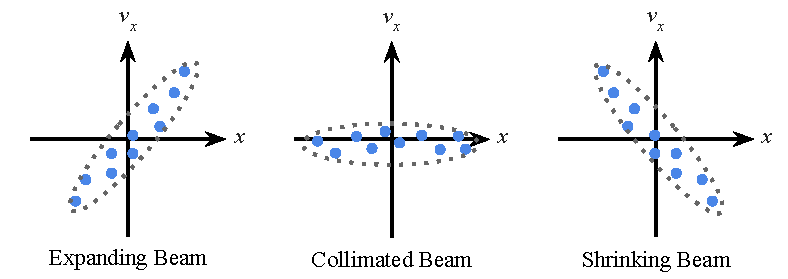
\includegraphics{part2/Figs/EmittanceExample.pdf}
\caption{An example of the trace-space occupied by an expanding, collimated and shrinking beam. The dotted line indicates the area occupied by the beam, the emittance.}
\label{figure:emittance_example}
\end{figure}

The density, $\rho$, of a beam of $N$ particles in trace space can usually be described by a Gaussian:
\begin{equation}\label{trace_space_density}
\rho(x, x^\prime) = N exp\left[ \frac{-(\sigma_{22}x^2-2\sigma_{12}xx^\prime+\sigma_{11}x^{\prime2}}{2|\sigma|} \right]
\end{equation}
where $|\sigma|$ is the determinant of the symmetric beam matrix,
\begin{equation}
\sigma = \begin{pmatrix} \sigma_{11} & \sigma_{12} \\ \sigma_{21} & \sigma_{22} \end{pmatrix}.
\end{equation}
$\sigma_{11}$ is the standard deviation of $x$, $\sigma_{22}$ the standard deviation of $x^\prime$ and $\sigma_{12}=\sigma_{21}$ indicates the coupling between $x$ and $x^\prime$. The \emph{emittance} can also be defined as
\begin{equation}\label{eq:emittancewithdeterminant}
\epsilon^x \equiv \sqrt{|\sigma|} = \sqrt{\sigma_{11}\sigma_{22}-\sigma_{12}^2}
\end{equation}

The \emph{\gls{rms} emittance} is a more practical measure and is defined as
\begin{equation}\label{emittance}
\epsilon \equiv \sqrt{\langle x^2\rangle \langle x^{\prime 2}\rangle - \langle x x^\prime\rangle^2}.
\end{equation}

The emittance of a beam represents the `focusability' of the beam.
A low emittance beam can be focused to a small waist than a high emittance beam, in fact a beam with zero emittance could be focused to a point whereas any beam with non-zero emittance has a finite spot size, this is shown in Figure~\ref{figure:focusability}.
This makes emittance an important quantity to consider in almost all beam applications but is particularly important to charged beams due to complications produced by space-charge repulsion.

\begin{figure}
\center
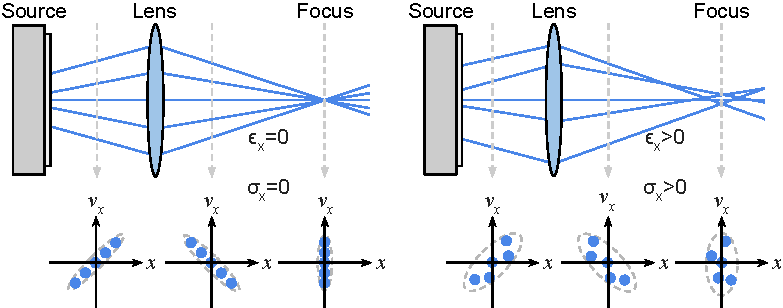
\includegraphics{part2/Figs/EmittanceFocasability.pdf}
\caption{On the left is a particle beam with zero emittance, and thus can be focused to a beam waist of zero width. On the right is a beam with non-zero emittance and thus a non-zero beam waist. Below each figure are plots of the phase space at difference points in the beam where the dashed line is indicative of the phase-space area or emittance.}
\label{figure:focusability}
\end{figure}

The emittance of a beam is not the only factor that determines the quality of the beam.
Emittance could be made arbitrarily small through the use of collimating slits however the reduced particle could would reduce the usefulness of that beam for most applications.
A more comprehensive figure of merit is the number of particles with a given emittance, known as \emph{brightness}~\cite{reiser_theory_2008};
\begin{equation}
B = \frac{I}{8\pi^2\epsilon_x\epsilon_y},
\end{equation}
where $I$ is the current of the beam and $\epsilon_{x,y}$ is the emittance as described above.
Brightness provides a better metric of a beam's quality with the additional requirement of knowing the beam current.

When comparing the emittance and brightness of particle beams from different sources it is often useful to use the \emph{normalised} emittance and brightness
\begin{align}
\bar{\epsilon_x} = \beta\epsilon_x,\\
\bar{B} = \frac{I}{8\pi^2\bar{\epsilon_x}\bar{\epsilon_y}}
\end{align}
where $\beta=v/c\approx v_z/c$.


\subsection{Emittance with a CAEIS}
\label{section:excess_energy_emittance}

For a \gls{caes} the normalised \gls{rms} emittance at the source is given by~\cite{mcculloch_high-coherence_2013}
\begin{equation}\label{equation:excess_energy_emittance}
\epsilon_x = \sigma_x \sqrt{\frac{k_B T}{m c^2}}
\end{equation}
where $\sigma_x$ is the \gls{rms} beam radius, $k_B$ is Boltzmann's constant, $T$ is the temperature of the source, $m$ is the particle mass and $c$ is the speed of light.
Equation~\ref{equation:excess_energy_emittance} highlights one of the advantages of a \gls{caeis} as the low source temperature allows for low emittance bunches compared to the common thermionic sources.

The temperature of the \gls{caeis} source can be calculated from the wavelength of the ionisation lasers, $\lambda_{red}$ and $\lambda_{blue}$,
\begin{align}
 E_{red} &= \frac{hc}{\lambda_{red}} \\
 E_{blue}&= \frac{hc}{\lambda_{blue}},
\end{align}
where $h$ is Plank's constant.
We can define the total ionisation energy to be
\begin{align}
E_{total} = E_{red} + E_{blue}.
\end{align}
The ionisation energy for Rubidium 85, $E_I$ is \unit[4.18]{eV} so we can determine the excess energy of ionisation
\begin{equation}
E_{excess} = E_{total} - E_I
\end{equation}

The excess energy can be related to the temperatures of the ionised particles via
\begin{equation}\label{equation:excess_energy_temperature}
T = \frac{E_{excess}}{k_B}.
\end{equation}
Combining Equations \ref{equation:excess_energy_emittance} and \ref{equation:excess_energy_temperature} allows for the calculation of the expected emittance of bunches generated from the \gls{caeis} for above-threshold ionisation.
The emittance of bunches generated from below-threshold pathways, such as Rydberg-excitation with field-ionisation, cannot be calculated using Equation~\ref{equation:excess_energy_emittance}.

\section{Measurement}

Directly calculating the emittance of an ensemble with Equation~\ref{emittance} requires full knowledge of the position and momenta of the particles which is difficult as beam monitors tend to only measure the transverse positions of particles.
There are a number of methods to practically calculate the emittance of a particle beam, namely pepperpots, the multiple profile method methods and the quadrupole method.

{\color{red}Is it worth mentioning multi-profile and quadrupole methods? I never used them.... I have data to \emph{attempt} multi-profile. Consider just removing those sections.}

\subsection{Pepperpots}

The pepperpot method uses a beam mask, consisting of an array of small holes, to obscure the beam which is then propagated and detected downstream.
by examining the size of the spots on the detector the divergence of the beam can be estimated and thus the emittance of the beam can be calculated.
Ideally the extent of the array should be larger than the size of the beam and the holes are as small as is practical while maintaining sufficient flux and ensuring the spots on the detector do not overlap.
The name refers to the similarity of the simplest beam mask to the perforated lid of a container for pepper.

A useful derivation of this technique is presented in Ref.~\cite{zhang_emittance_1996} with the one dimensional result:

\begin{dmath}\label{equation:pepperpot}
\epsilon_x^2 = \left\langle x^2\right\rangle \left\langle x^{\prime2}\right\rangle - \left\langle xx^\prime\right\rangle^2\allowbreak
\approx \frac{1}{N^2} \left\{\left[\sum_{j=1}^p{n_j\left(x_{sj}-\bar{x}\right)^2}\right] \left[ \sum_{j=1}^p{\left[n_j\sigma_{x_j^\prime}^2 + n_j\left(\bar{x_j^\prime}-\bar{x^\prime}\right)^2\right]}\right] - \left[ \sum_{j=1}^p{n_jx_{sj}\bar{x_j^\prime}-N\bar{x}\bar{x^\prime}}\right]^2\right\}
\end{dmath}
where;
\begin{itemize}
    \item $N$ is the total number of particles after the beam mask,
    \item $p$ is the total number of holes in the $x$ direction,
    \item $n_j$ is the number of particles passing through the $j$-th hole and hitting the detector,
    \item $x_{sj}$ is position of the $j$-th hole,
    \item $\bar{x}$ is the mean position of the holes,
    \item $\sigma_{x_j^\prime}$ is the \gls{rms} divergence of the $j$-th beamlet,
    \item $\bar{x_j^\prime}$ is the mean divergence of the $j$-th beamlet, and
    \item $\bar{x^\prime}$ is the mean divergence of all beamlets.
\end{itemize}

An example pepperpot mask and detected beamlets are shown in Figure~\ref{figure:pepperpot_example}.
This equation can be implemented by appropriately rotating the detected beamlets and then performing row and column sums of the pixels followed by application of Equation~\ref{equation:pepperpot} for $x$ and $y$.

\begin{figure}
    \centering
    \begin{subfigure}{0.49\linewidth}
    \centering
    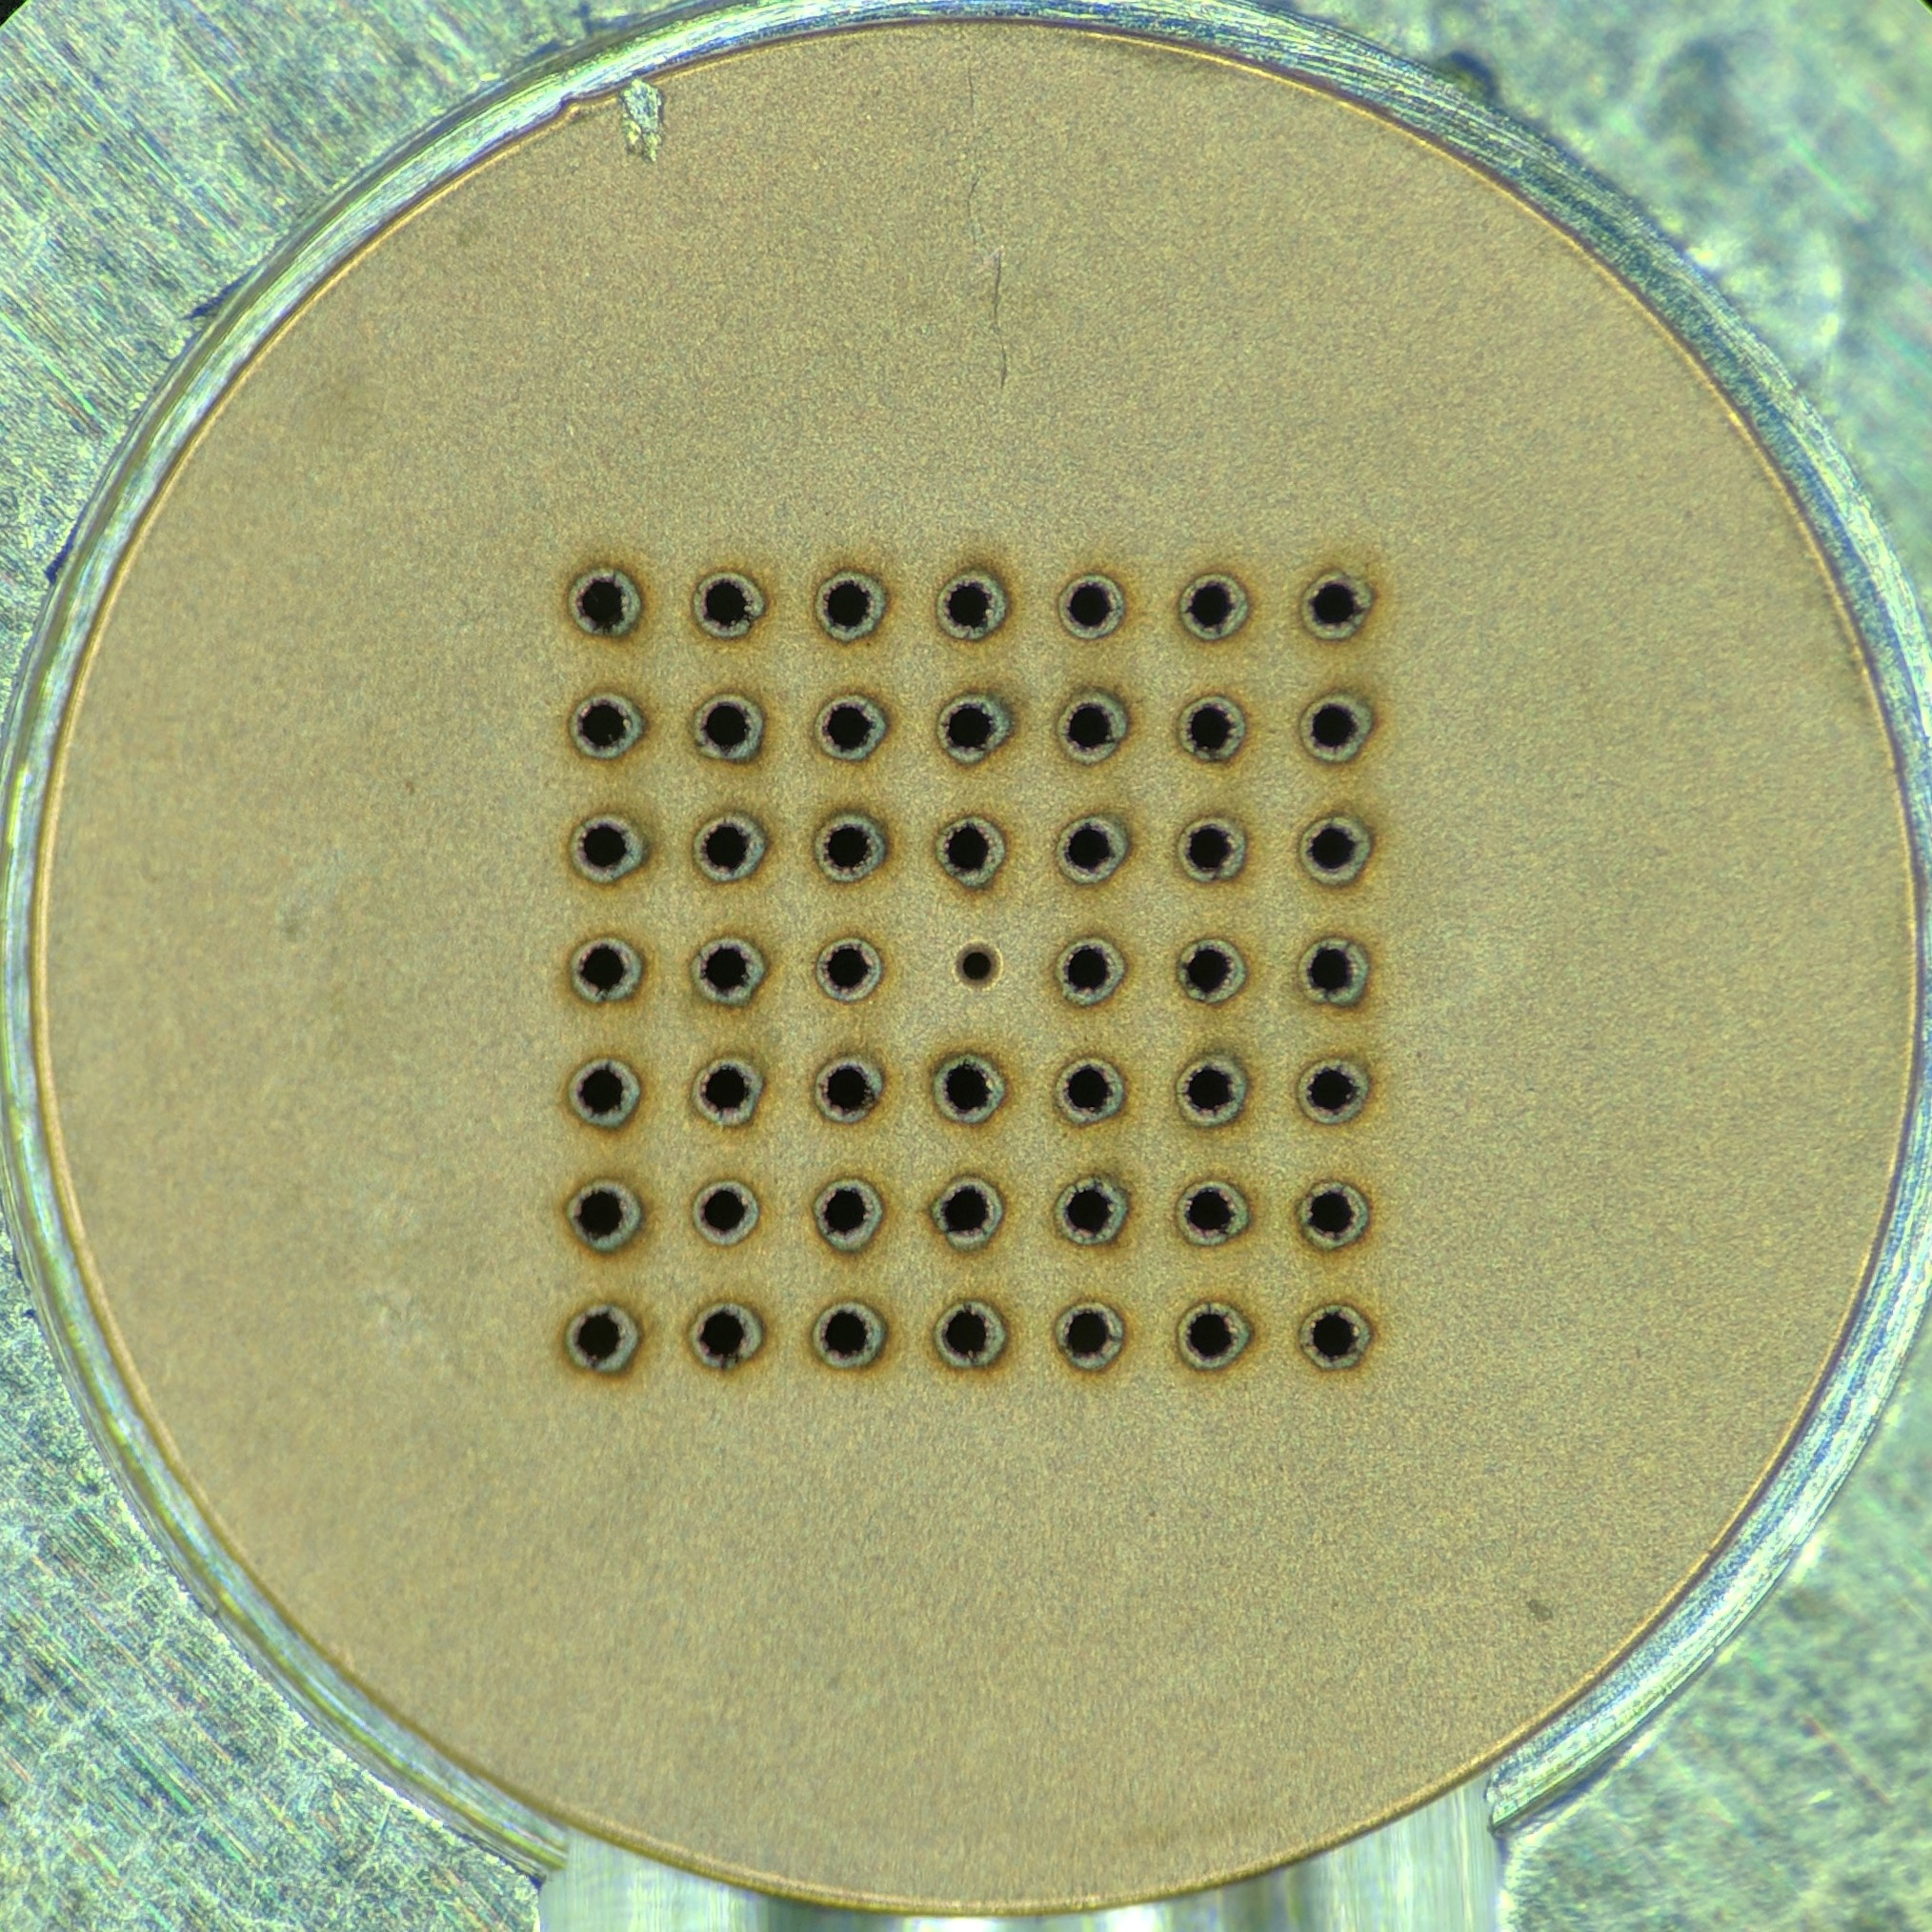
\includegraphics[width=\linewidth]{part2/Figs/example_pepperpot_mask.jpg}
    \caption{}
    \label{figure:pepperpot_mask}
    \end{subfigure}
    \begin{subfigure}{0.49\linewidth}
    \centering
    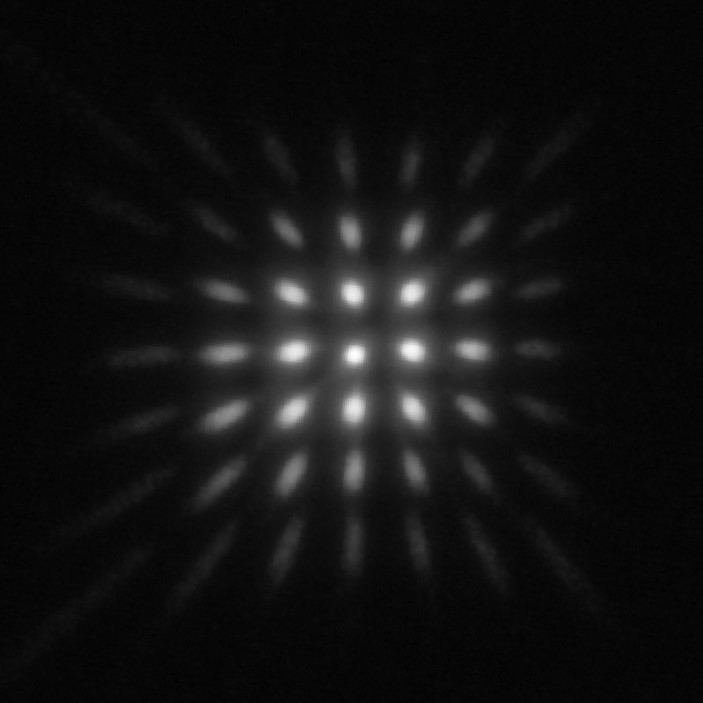
\includegraphics[width=\linewidth]{part2/Figs/example_pepperpot_detector_linear.jpeg}
    % 486.971 pepperpot from 2017.06.06
    \caption{}
    \label{figure:pepperpot_image}
    \end{subfigure}
    
    \begin{subfigure}{0.49\linewidth}
    \centering
    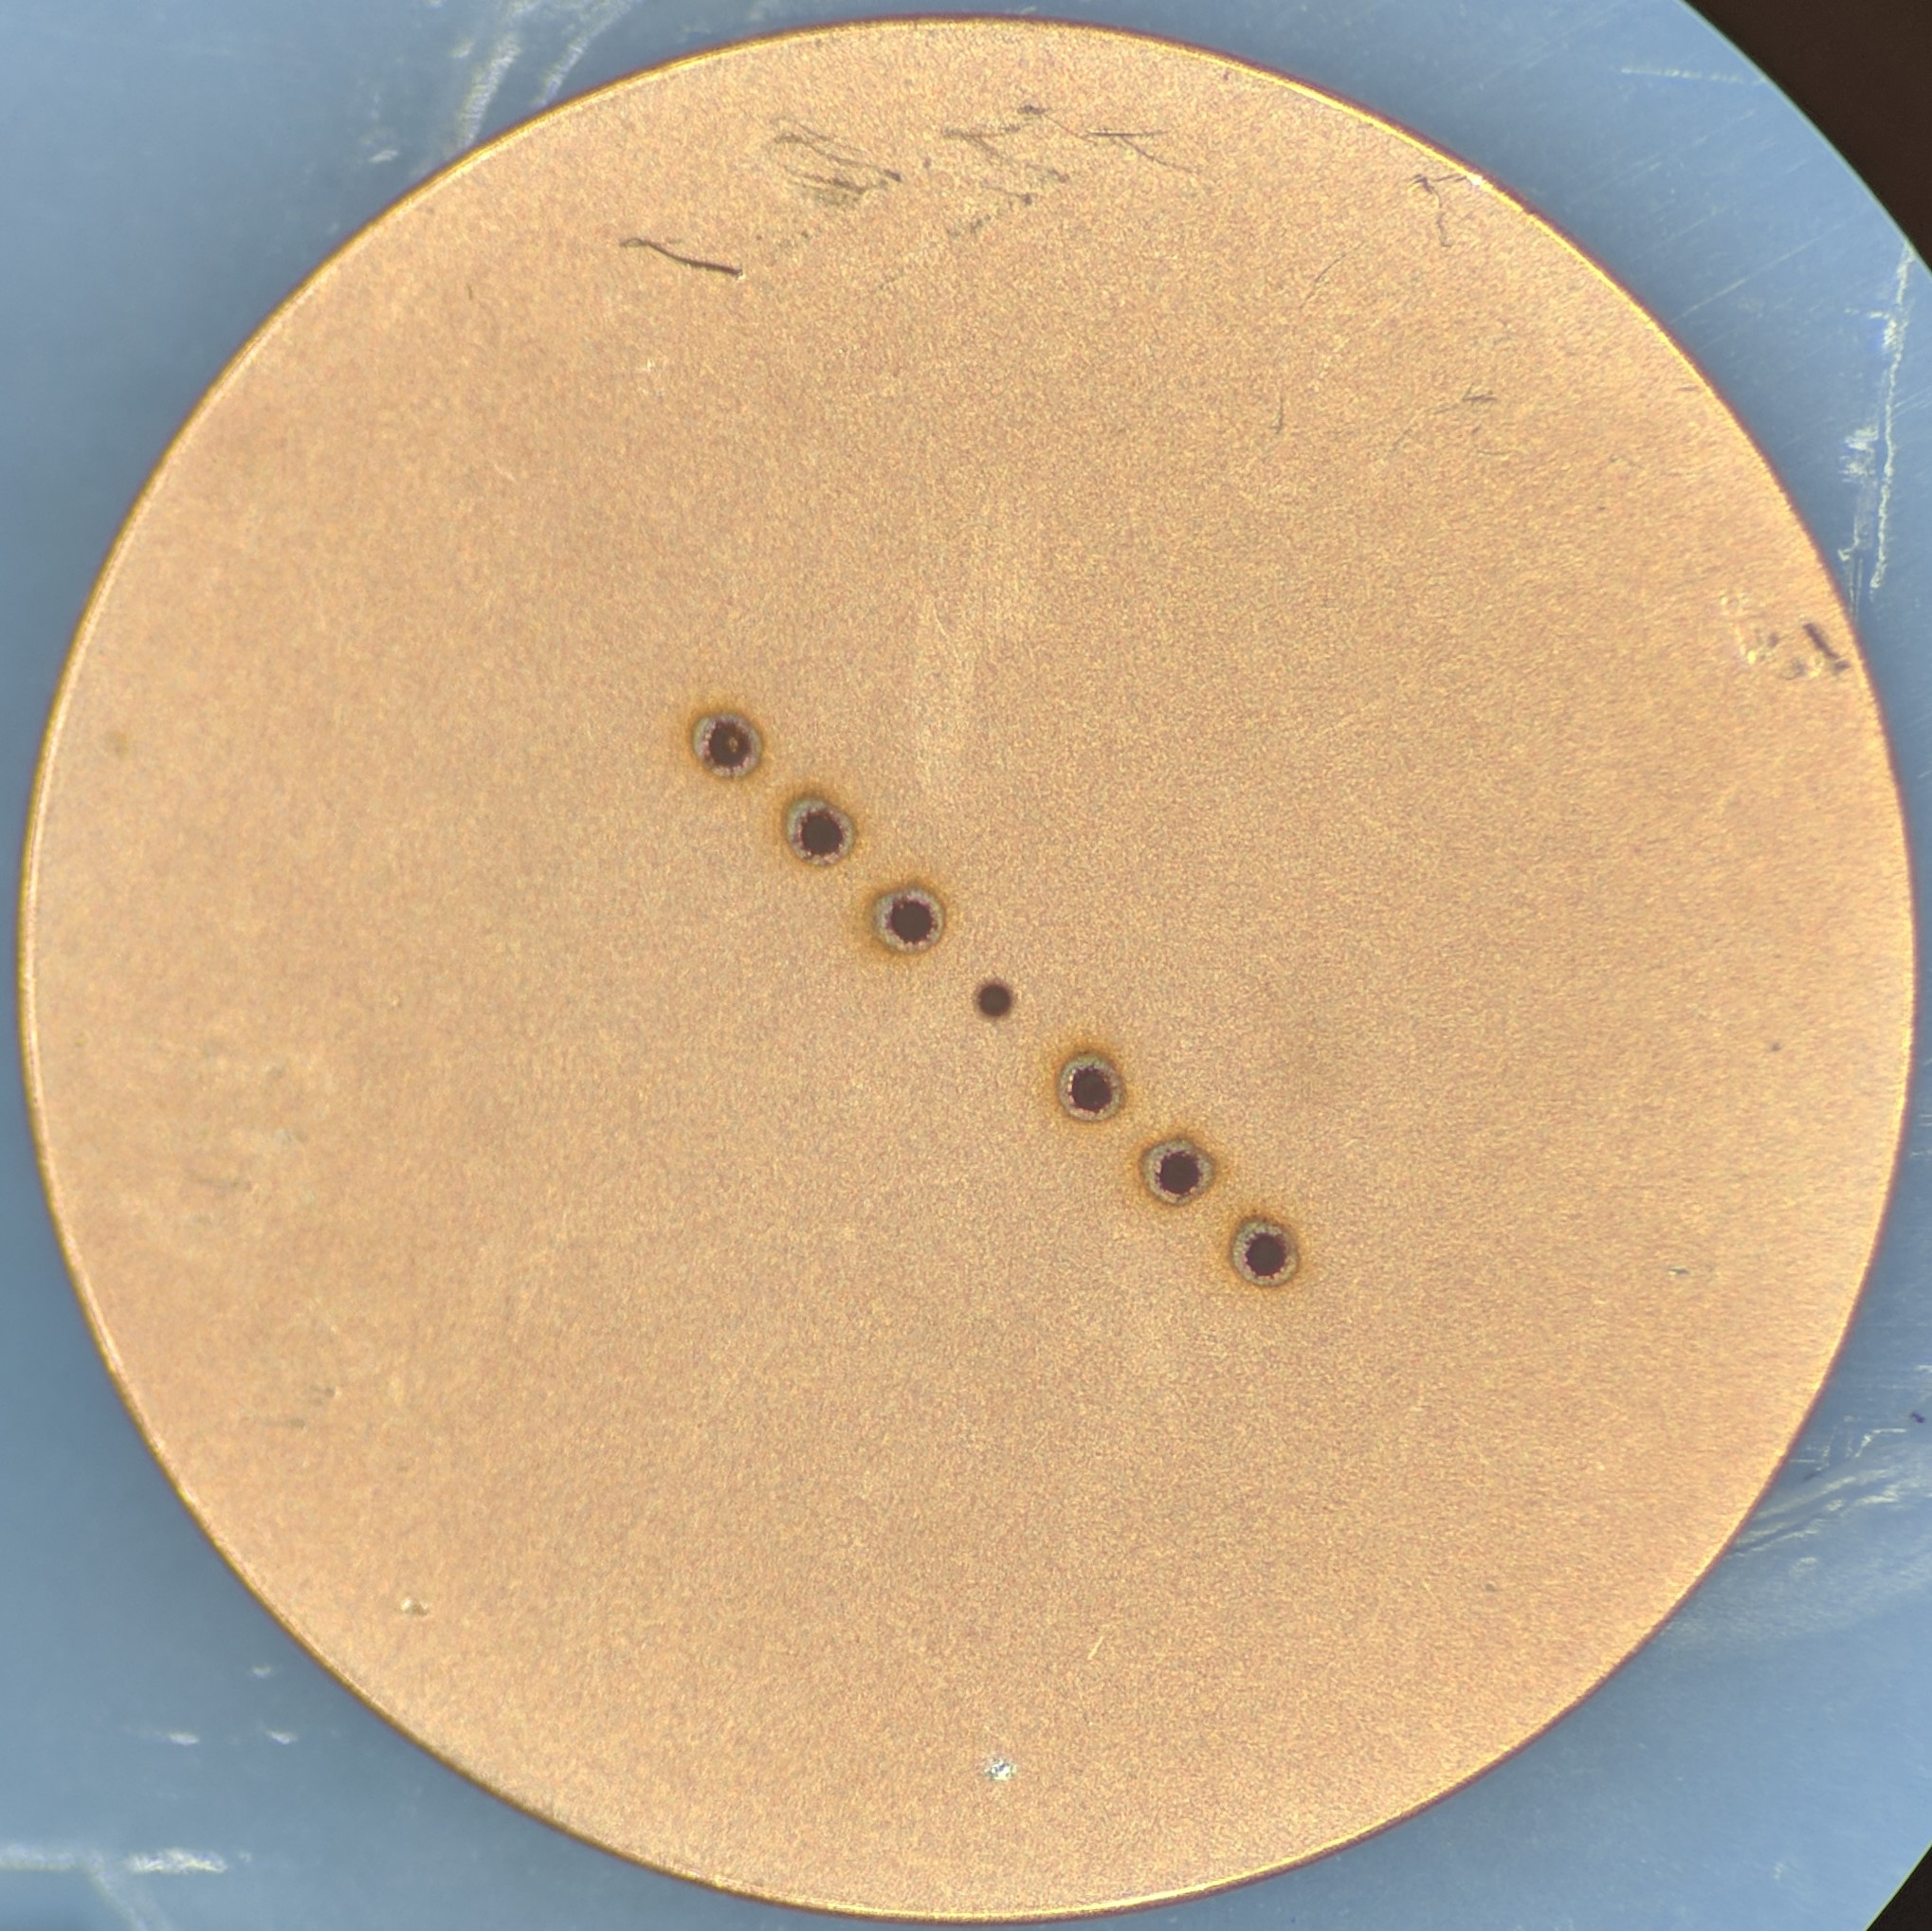
\includegraphics[width=\linewidth]{part2/Figs/example_pepperpot_1d.jpg}
    \caption{}
    \label{figure:1d_pepperpot}
    \end{subfigure}
    \begin{subfigure}{0.49\linewidth}
    \centering
    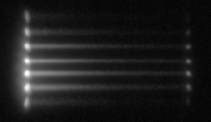
\includegraphics[width=\linewidth]{part2/Figs/example_streaked_pepperpot.png}
    \caption{}
    \label{figure:streaked_1d_pepperpot}
    \end{subfigure}
    % Manual labels.....
    \caption{(a) a pepperpot mask cut into a thing copper disk and, (b), the corresponding set of beamlets on the detector. (c) a one-dimensional pepperpot mask (held in place by a copper ring) and the corresponding streaked set of beamlets on the detector, (d). The beam images are log scaled.}
    \label{figure:pepperpot_example}
\end{figure}

\subsubsection{Temporal Resolution with Streaking}
A one-dimensional pepperpots can consist of a line of apertures and provide a prime target for a streak measurements.
In this case streaking is performed with a time varying electric field which deflects the charged particles across the detector, providing time-resolution.
For a pulsed charged particle source, such as the \gls{caeis}, the streak can be performed over the duration of the bunch or over a portion of the bunch if higher resolution is required.
There are some considerations for how fast an electric field can be swept, which will not be examined in detail here, so extremely short bunches will require more complicated systems, such as a \gls{rf} cavity, to provide the appropriate timing and electric field temporal-gradient~\cite{alesini_rf_2006}.
An example of a streaked pepperpot measurement is shown in Figure~\ref{figure:streaked_1d_pepperpot}.

\subsection{Multi-profile Method}

If a beam can be described by $\sigma^0$ at $z_0$ and by $\sigma^1$ at $z_1$ then the transformation matrix, $\mathbf{R}_{12}$ from $z_0$ to $z_1$ is
\begin{equation}
\mathbf{R} = \begin{pmatrix} R_{11} & R_{12} \\ R_{21} & R_{22} \end{pmatrix}
\end{equation}
and
\begin{equation}
\sigma^1 = \mathbf{R}\sigma^0\mathbf{R}^T
\end{equation}
where $\mathbf{R}^T$ is the transpose of $\mathbf{R}$.
The combined transfer matrix for a series of $z$ positions is simply the product of the individual transfer matrices.

We can write:
\begin{equation}\label{equation:multiprofile}
\sigma_{11}^1 = R_{11}^2\sigma_{11}^0 + 2R_{11}R_{12}\sigma_{12}^0 + R_{12}^2\sigma_{22}^0
\end{equation}

Typical detectors are only able to measure the standard deviation of $x$, $\sigma_{11}$.
With at least three measurements and known transfer matrices the other elements of $\sigma$ can be determined.
With more than three measurements uncertainty can be reduced.

The transfer matrix for simple propagation over a distance $L$ is
\begin{equation}
\mathbf{R}_L = \begin{pmatrix}1 & L \\ 0 & 1\end{pmatrix}
\end{equation}
and then Equation~\ref{equation:multiprofile} becomes
\begin{equation}
\sigma_{11}^1 = \sigma_{11}^0 + 2L \sigma_{12}^0 + L_1^2\sigma_{22}^0.
\end{equation}

\begin{figure}
\center
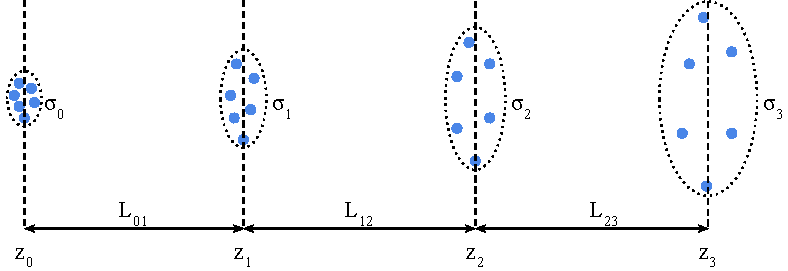
\includegraphics{part2/Figs/Multi-ProfileEmittance.pdf}
\caption{An example of a multi-profile emittance measurement conducted on an expanding beam travelling from left to right (or a shrinking beam travelling right to left).}
\label{figure:multiprofileexample}
\end{figure}

With an initial beam, $\sigma_0$, measured at $z_1, z_2$ and $z_3$ as shown in Figure~\ref{figure:multiprofileexample} then $\sigma_{11}^1$, $\sigma_{11}^2$, and $\sigma_{11}^3$ are know and we can write 
\begin{align}
\sigma_{11}^1 &= \sigma_{11}^0 +2L_{01}\sigma_{12}^0 + L_{01}^2\sigma_{22}^0 \notag\\
\sigma_{11}^2&= \sigma_{11}^0+2(L_{01}+L_{12})\sigma_{12}^0 + (L_{01}+L_{12})^2\sigma_{22}^0 \notag\\
\sigma_{11}^3&= \sigma_{11}^0+2(L_{01}+L_{12}+L_{23})\sigma_{12}^0 + (L_{01}+L_{12}+L_{23})^2\sigma_{22}^0 \label{eq:multiprofilesolution}
\end{align}

Which can easily be solved for $\sigma_0$ thus allowing the calculation of the emittance with Equation~\ref{eq:emittancewithdeterminant}.

This method is feasible with the \gls{caeis} at the University of Melbourne but labourious due to the manual operation of the bellows the detector is attached to.

\subsection{Quadrupole Method}

The quadrupole method is similar to the multi-profile method but requires only a single location to measure the beam width and a well characterised variable lens such as a quadrupole lens.
A quadrupole lens with a magnetic field gradient of $G$ has the transfer matrix in the focusing plane of
\begin{equation}
\mathbf{R}_f = \begin{pmatrix} \cos kl & (1/k)\sin kl\\
-k\sin kl & cos kl\end{pmatrix},
\end{equation}
where $l$ is the effective length of the quadrupole, $k^2=G/B\rho$ is the quadrupole strength and $B\rho$ is the magnetic rigidity of the particles in the assumed central trajectory.
The matrix in the defocusing plane is
\begin{equation}
\mathbf{R}_d = \begin{pmatrix} \cosh kl & (1/k) \sin kl\\
k \sinh kl & \cosh kl \end{pmatrix}
\end{equation}

A beam measured a distance $L$ away from the quadrupole will have undergone the transformation $\mathbf{R}=\mathbf{R}_L\mathbf{R}_f$ on one axis and $\mathbf{R}=\mathbf{R}_L\mathbf{R}_d$ on the other.
The symmetric beam matrix for the beam before the lens can then be determined from a series of beam profile measurements with different focusing strengths.
The main advantage of this measurement is that is only requires a single beam monitor location.

Due to the ad hoc nature of the magnetic lenses used in the \gls{caes} this method is not practical without a thorough characterisation of the lenses, especially in comparison with the ease of the alternative methods.

\section{Experimental Setup}

A number of modifications were made to the \gls{caeis} to prepare it for the streaked emittance measurements and there were a number of restrictions on various parameters due to the precise setup of the apparatus.
The \gls{caeis} was operated in electron mode for these measurements due to the available magnetic optics and the larger emittance expected from electrons as the source temperature is higher for electrons, a minimum temperature of approximately \unit[10]{K} for electrons and \unit[100]{$\mu K$} for ions~\cite{saliba_spatial_2012}.
Using electrons also allows some control of the bunch emittance as the excess energy can be controlled with the blue ionisation laser wavelength, with ions the change in emittance would be negligible.

See Chapter~\ref{chapter:setup} for a more detailed description of the \gls{caeis} and Figure~\ref{figure:emittance_schematic} for a schematic of the setup used for the measurements in this chapter.

\begin{figure}
\center
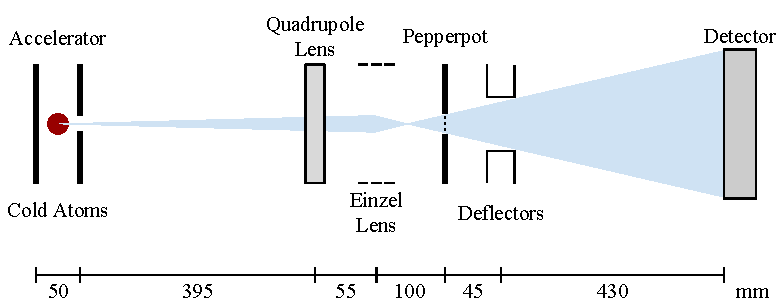
\includegraphics{part2/Figs/EmittanceApparatusSchematic.pdf}
\caption{A schematic of the experimental apparatus with relevant dimensions. The blue region indicates the electron beam envelope. Note that components are not necessarily orientate realistically in this schematic (particularly the deflectors).}
\label{figure:emittance_schematic}
\end{figure}

\subsection{Beam Optics}
The quadrupole electron optics discussed in Section \ref{section:quadrupole} were use to reduce the astigmatism present in the electron beam as discussed in the aforementioned section.
The two-dimensional pepperpot provide another avenue to monitor the astigmatism of the beam as with an astigmatic beam the spacing of the beamlets on the detector are not the same along each axis as shown in Figure~\ref{figure:astigmatic_pepperpot}.
When focussing was required the Einzel lens was used.

\begin{figure}
    \center
    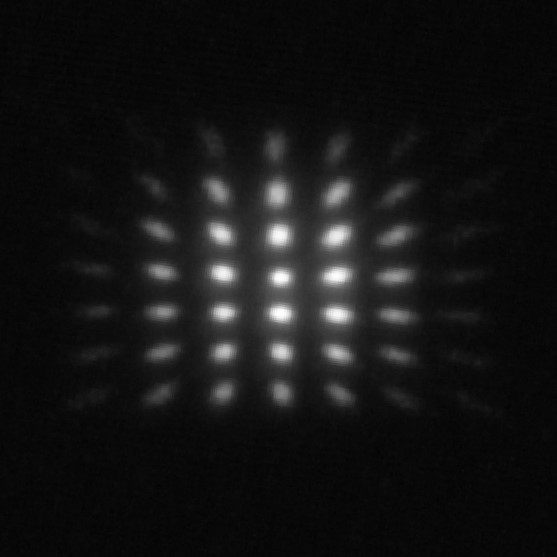
\includegraphics[width=0.5\linewidth]{part2/Figs/example_astigmatic_pepperpot.jpeg}
    \caption{An example of a pepperpot without the beam correction from the quadrupole lens. It is readily apparent that spacing of the beamlets is not the same for the $x$ and $y$ axes. This image is log scaled.}
    \label{figure:astigmatic_pepperpot}
    % From 2017.06.01
\end{figure}

A number of permanent magnets were used to steer the beam through the various apertures and onto the detector and care was taken to attempt to keep the beam on the central axis of the apparatus.
This was achieved by manually adjusting the positions of the magnets, which were mounted on posts external to the vacuum system, to ensure that the beam was passing through the apertures in the system and by scanning the Einzel lens to verify that the beam was passing through its centre.
Due to the unstable nature of the apparatus these magnets needed to be adjusted on a day-to-day basis to maintain the beam path.

The main limiting factor to pepperpot emittance measurements using the \gls{caes} was electron flux through the pepperpot masks.
Flux through the pepperpot masks was maximised by using the Einzel lens to focus the beam to the approximate size of the pepperpots in the pepperpot plane, thus maximising the flux through the apertures.
The Einzel lens voltage required for this was approximately \unit[4.8][kV] and varied slightly beam emittance, i.e.. high emittance beams result in a larger beam size and thus required adjusting the Einzel lens voltage by \unit[100]{V} or so.

\subsection{Beam Energy}
In many emittance measurements the beam energy would not be a free parameter as it will be used as a diagnostic for a specific system or scenario, however in this experiment we are able to vary the energy of our beam from a few hundred eV to around \unit[10]{keV}.
There are a number of considerations in determining the optimal beam energy to use for pepperpot measurements such as measurement resolution, beam current and beam stability.

The resolution of a pepperpot measurement is greater when the size of the beamlets on the detector is larger and, as shown in Equation~\ref{equation:divergence} the divergence is greater for slower beams.
Unfortunately the slower the beam the more fragile the alignment of the beam becomes.
While attempting to align a \unit[500][eV] beam through it system it was impossible to position the steering magnets such that an unobstructed beam made it through the system to the detector.

A relatively high energy beam of \unit[8]{keV} was used as this provided a robust beam alignment that was resistant to the transient changes in the magnetic environment while providing sufficient measurement resolution.

\subsection{Bellows}

The bellows provide an additional mechanism to control the resolution of the measurement by adjusting the propagation distance of the pepperpot beamlets and thus their size on the detector.
As this parameter is also adjustable with the strength of the Einzel lens the bellows were placed approximately halfway between the minimum and maximum position where the beam alignment was still well behaved.

{\color{red}Add photo of bellows}

\subsection{Streaking}
The streaking was performed using a pair of deflectors located after the pepperpot sample and orientated such that the one-dimensional pepperpots could be streaked across the detector.
For these measurements one deflector was grounded and the other given a time-varying voltage which was supplied in one of two ways:
\begin{itemize}
\item A fast ramp using a bipolar push-pull solid-state switch with a fixed transition time of \unit[10]{ns} and
\item A slower ramp using an amplified signal generator with a minimum transition of approximately \unit[10]{$\mu$s}.
\end{itemize}
An example of the voltage ramps is shown in Figure~\ref{figure:deflector_voltages}. The slow ramp was done by amplifying the output of signal generator\footnote{Rigol DG4162, able to operate up to \unit[160]{MHz}} which is highly configurable and thus capable of a wide range of pulse lengths, limited by the speed of the amplifier to a transition time approximately \unit[10]{$\mu$s} in duration as shown in Figure~\ref{figure:deflector_voltages}.
More detail on the design of the streaking electronics can be found in Reference~{\color{red}(Cite Rory's thesis)}.

\begin{figure}
    \center
    %% Creator: Matplotlib, PGF backend
%%
%% To include the figure in your LaTeX document, write
%%   \input{<filename>.pgf}
%%
%% Make sure the required packages are loaded in your preamble
%%   \usepackage{pgf}
%%
%% Figures using additional raster images can only be included by \input if
%% they are in the same directory as the main LaTeX file. For loading figures
%% from other directories you can use the `import` package
%%   \usepackage{import}
%% and then include the figures with
%%   \import{<path to file>}{<filename>.pgf}
%%
%% Matplotlib used the following preamble
%%
\begingroup%
\makeatletter%
\begin{pgfpicture}%
\pgfpathrectangle{\pgfpointorigin}{\pgfqpoint{5.710000in}{1.903333in}}%
\pgfusepath{use as bounding box, clip}%
\begin{pgfscope}%
\pgfsetbuttcap%
\pgfsetmiterjoin%
\definecolor{currentfill}{rgb}{1.000000,1.000000,1.000000}%
\pgfsetfillcolor{currentfill}%
\pgfsetlinewidth{0.000000pt}%
\definecolor{currentstroke}{rgb}{1.000000,1.000000,1.000000}%
\pgfsetstrokecolor{currentstroke}%
\pgfsetdash{}{0pt}%
\pgfpathmoveto{\pgfqpoint{0.000000in}{0.000000in}}%
\pgfpathlineto{\pgfqpoint{5.710000in}{0.000000in}}%
\pgfpathlineto{\pgfqpoint{5.710000in}{1.903333in}}%
\pgfpathlineto{\pgfqpoint{0.000000in}{1.903333in}}%
\pgfpathclose%
\pgfusepath{fill}%
\end{pgfscope}%
\begin{pgfscope}%
\pgfsetbuttcap%
\pgfsetmiterjoin%
\definecolor{currentfill}{rgb}{1.000000,1.000000,1.000000}%
\pgfsetfillcolor{currentfill}%
\pgfsetlinewidth{0.000000pt}%
\definecolor{currentstroke}{rgb}{0.000000,0.000000,0.000000}%
\pgfsetstrokecolor{currentstroke}%
\pgfsetstrokeopacity{0.000000}%
\pgfsetdash{}{0pt}%
\pgfpathmoveto{\pgfqpoint{0.661914in}{0.570703in}}%
\pgfpathlineto{\pgfqpoint{3.110957in}{0.570703in}}%
\pgfpathlineto{\pgfqpoint{3.110957in}{1.753333in}}%
\pgfpathlineto{\pgfqpoint{0.661914in}{1.753333in}}%
\pgfpathclose%
\pgfusepath{fill}%
\end{pgfscope}%
\begin{pgfscope}%
\pgfpathrectangle{\pgfqpoint{0.661914in}{0.570703in}}{\pgfqpoint{2.449043in}{1.182630in}} %
\pgfusepath{clip}%
\pgfsetrectcap%
\pgfsetroundjoin%
\pgfsetlinewidth{1.003750pt}%
\definecolor{currentstroke}{rgb}{0.309804,0.478431,0.682353}%
\pgfsetstrokecolor{currentstroke}%
\pgfsetdash{}{0pt}%
\pgfpathmoveto{\pgfqpoint{0.661914in}{0.639863in}}%
\pgfpathlineto{\pgfqpoint{0.685907in}{0.638678in}}%
\pgfpathlineto{\pgfqpoint{0.688437in}{0.638833in}}%
\pgfpathlineto{\pgfqpoint{0.691552in}{0.639256in}}%
\pgfpathlineto{\pgfqpoint{0.710846in}{0.640263in}}%
\pgfpathlineto{\pgfqpoint{0.712757in}{0.639892in}}%
\pgfpathlineto{\pgfqpoint{0.716371in}{0.638523in}}%
\pgfpathlineto{\pgfqpoint{0.720898in}{0.639289in}}%
\pgfpathlineto{\pgfqpoint{0.723118in}{0.639239in}}%
\pgfpathlineto{\pgfqpoint{0.725751in}{0.638742in}}%
\pgfpathlineto{\pgfqpoint{0.730157in}{0.640450in}}%
\pgfpathlineto{\pgfqpoint{0.733238in}{0.640418in}}%
\pgfpathlineto{\pgfqpoint{0.735820in}{0.640113in}}%
\pgfpathlineto{\pgfqpoint{0.741534in}{0.638183in}}%
\pgfpathlineto{\pgfqpoint{0.743806in}{0.638528in}}%
\pgfpathlineto{\pgfqpoint{0.747042in}{0.639045in}}%
\pgfpathlineto{\pgfqpoint{0.752498in}{0.639197in}}%
\pgfpathlineto{\pgfqpoint{0.756921in}{0.640379in}}%
\pgfpathlineto{\pgfqpoint{0.760088in}{0.639106in}}%
\pgfpathlineto{\pgfqpoint{0.764064in}{0.638800in}}%
\pgfpathlineto{\pgfqpoint{0.769313in}{0.639684in}}%
\pgfpathlineto{\pgfqpoint{0.783805in}{0.639351in}}%
\pgfpathlineto{\pgfqpoint{0.792015in}{0.641048in}}%
\pgfpathlineto{\pgfqpoint{0.796215in}{0.640030in}}%
\pgfpathlineto{\pgfqpoint{0.807867in}{0.639090in}}%
\pgfpathlineto{\pgfqpoint{0.810448in}{0.639002in}}%
\pgfpathlineto{\pgfqpoint{0.816782in}{0.640631in}}%
\pgfpathlineto{\pgfqpoint{0.819278in}{0.639510in}}%
\pgfpathlineto{\pgfqpoint{0.821636in}{0.639273in}}%
\pgfpathlineto{\pgfqpoint{0.824338in}{0.639420in}}%
\pgfpathlineto{\pgfqpoint{0.826989in}{0.638791in}}%
\pgfpathlineto{\pgfqpoint{0.830242in}{0.639425in}}%
\pgfpathlineto{\pgfqpoint{0.836420in}{0.639113in}}%
\pgfpathlineto{\pgfqpoint{0.840482in}{0.638745in}}%
\pgfpathlineto{\pgfqpoint{0.842806in}{0.639399in}}%
\pgfpathlineto{\pgfqpoint{0.845181in}{0.639797in}}%
\pgfpathlineto{\pgfqpoint{0.849123in}{0.639023in}}%
\pgfpathlineto{\pgfqpoint{0.852668in}{0.639534in}}%
\pgfpathlineto{\pgfqpoint{0.857264in}{0.639722in}}%
\pgfpathlineto{\pgfqpoint{0.862427in}{0.640019in}}%
\pgfpathlineto{\pgfqpoint{0.865886in}{0.639236in}}%
\pgfpathlineto{\pgfqpoint{0.871790in}{0.639947in}}%
\pgfpathlineto{\pgfqpoint{0.874303in}{0.639239in}}%
\pgfpathlineto{\pgfqpoint{0.878933in}{0.639722in}}%
\pgfpathlineto{\pgfqpoint{0.886024in}{0.640670in}}%
\pgfpathlineto{\pgfqpoint{0.900481in}{0.665955in}}%
\pgfpathlineto{\pgfqpoint{0.914991in}{0.692189in}}%
\pgfpathlineto{\pgfqpoint{0.984335in}{0.811283in}}%
\pgfpathlineto{\pgfqpoint{0.986934in}{0.815749in}}%
\pgfpathlineto{\pgfqpoint{0.995781in}{0.831818in}}%
\pgfpathlineto{\pgfqpoint{1.009602in}{0.855721in}}%
\pgfpathlineto{\pgfqpoint{1.013491in}{0.861243in}}%
\pgfpathlineto{\pgfqpoint{1.023181in}{0.875697in}}%
\pgfpathlineto{\pgfqpoint{1.031236in}{0.887602in}}%
\pgfpathlineto{\pgfqpoint{1.044506in}{0.905297in}}%
\pgfpathlineto{\pgfqpoint{1.051305in}{0.916597in}}%
\pgfpathlineto{\pgfqpoint{1.099256in}{0.993578in}}%
\pgfpathlineto{\pgfqpoint{1.105572in}{1.002734in}}%
\pgfpathlineto{\pgfqpoint{1.121028in}{1.028128in}}%
\pgfpathlineto{\pgfqpoint{1.134109in}{1.047792in}}%
\pgfpathlineto{\pgfqpoint{1.137121in}{1.053476in}}%
\pgfpathlineto{\pgfqpoint{1.139995in}{1.056965in}}%
\pgfpathlineto{\pgfqpoint{1.142990in}{1.060511in}}%
\pgfpathlineto{\pgfqpoint{1.160460in}{1.089288in}}%
\pgfpathlineto{\pgfqpoint{1.198376in}{1.148417in}}%
\pgfpathlineto{\pgfqpoint{1.201302in}{1.153386in}}%
\pgfpathlineto{\pgfqpoint{1.205037in}{1.159542in}}%
\pgfpathlineto{\pgfqpoint{1.213677in}{1.171255in}}%
\pgfpathlineto{\pgfqpoint{1.220269in}{1.181702in}}%
\pgfpathlineto{\pgfqpoint{1.225588in}{1.189842in}}%
\pgfpathlineto{\pgfqpoint{1.236190in}{1.205469in}}%
\pgfpathlineto{\pgfqpoint{1.272230in}{1.255450in}}%
\pgfpathlineto{\pgfqpoint{1.276172in}{1.260278in}}%
\pgfpathlineto{\pgfqpoint{1.284846in}{1.273493in}}%
\pgfpathlineto{\pgfqpoint{1.301077in}{1.296105in}}%
\pgfpathlineto{\pgfqpoint{1.308288in}{1.305361in}}%
\pgfpathlineto{\pgfqpoint{1.312540in}{1.311632in}}%
\pgfpathlineto{\pgfqpoint{1.318237in}{1.319983in}}%
\pgfpathlineto{\pgfqpoint{1.331334in}{1.337047in}}%
\pgfpathlineto{\pgfqpoint{1.340715in}{1.348001in}}%
\pgfpathlineto{\pgfqpoint{1.360336in}{1.368650in}}%
\pgfpathlineto{\pgfqpoint{1.367186in}{1.371538in}}%
\pgfpathlineto{\pgfqpoint{1.369974in}{1.371728in}}%
\pgfpathlineto{\pgfqpoint{1.378580in}{1.372520in}}%
\pgfpathlineto{\pgfqpoint{1.382383in}{1.373033in}}%
\pgfpathlineto{\pgfqpoint{1.385671in}{1.372624in}}%
\pgfpathlineto{\pgfqpoint{1.391798in}{1.369904in}}%
\pgfpathlineto{\pgfqpoint{1.398751in}{1.367030in}}%
\pgfpathlineto{\pgfqpoint{1.401936in}{1.366306in}}%
\pgfpathlineto{\pgfqpoint{1.405051in}{1.365280in}}%
\pgfpathlineto{\pgfqpoint{1.412916in}{1.361527in}}%
\pgfpathlineto{\pgfqpoint{1.414620in}{1.360642in}}%
\pgfpathlineto{\pgfqpoint{1.418803in}{1.357469in}}%
\pgfpathlineto{\pgfqpoint{1.422830in}{1.356282in}}%
\pgfpathlineto{\pgfqpoint{1.449215in}{1.342742in}}%
\pgfpathlineto{\pgfqpoint{1.451763in}{1.341815in}}%
\pgfpathlineto{\pgfqpoint{1.458768in}{1.337920in}}%
\pgfpathlineto{\pgfqpoint{1.463879in}{1.335066in}}%
\pgfpathlineto{\pgfqpoint{1.482278in}{1.323278in}}%
\pgfpathlineto{\pgfqpoint{1.486289in}{1.321369in}}%
\pgfpathlineto{\pgfqpoint{1.489301in}{1.319998in}}%
\pgfpathlineto{\pgfqpoint{1.491676in}{1.318482in}}%
\pgfpathlineto{\pgfqpoint{1.496702in}{1.315281in}}%
\pgfpathlineto{\pgfqpoint{1.508027in}{1.307857in}}%
\pgfpathlineto{\pgfqpoint{1.512519in}{1.305661in}}%
\pgfpathlineto{\pgfqpoint{1.536133in}{1.292034in}}%
\pgfpathlineto{\pgfqpoint{1.538680in}{1.290625in}}%
\pgfpathlineto{\pgfqpoint{1.543672in}{1.287161in}}%
\pgfpathlineto{\pgfqpoint{1.552604in}{1.281694in}}%
\pgfpathlineto{\pgfqpoint{1.559127in}{1.277377in}}%
\pgfpathlineto{\pgfqpoint{1.588060in}{1.259416in}}%
\pgfpathlineto{\pgfqpoint{1.592190in}{1.256355in}}%
\pgfpathlineto{\pgfqpoint{1.601450in}{1.251964in}}%
\pgfpathlineto{\pgfqpoint{1.606958in}{1.249291in}}%
\pgfpathlineto{\pgfqpoint{1.611054in}{1.245824in}}%
\pgfpathlineto{\pgfqpoint{1.616700in}{1.243599in}}%
\pgfpathlineto{\pgfqpoint{1.621983in}{1.241119in}}%
\pgfpathlineto{\pgfqpoint{1.624186in}{1.240234in}}%
\pgfpathlineto{\pgfqpoint{1.631312in}{1.234378in}}%
\pgfpathlineto{\pgfqpoint{1.650606in}{1.225090in}}%
\pgfpathlineto{\pgfqpoint{1.657542in}{1.220294in}}%
\pgfpathlineto{\pgfqpoint{1.663824in}{1.217270in}}%
\pgfpathlineto{\pgfqpoint{1.669280in}{1.214376in}}%
\pgfpathlineto{\pgfqpoint{1.671948in}{1.211721in}}%
\pgfpathlineto{\pgfqpoint{1.674513in}{1.209897in}}%
\pgfpathlineto{\pgfqpoint{1.677783in}{1.209593in}}%
\pgfpathlineto{\pgfqpoint{1.684977in}{1.206012in}}%
\pgfpathlineto{\pgfqpoint{1.687111in}{1.204250in}}%
\pgfpathlineto{\pgfqpoint{1.689986in}{1.202495in}}%
\pgfpathlineto{\pgfqpoint{1.693721in}{1.200464in}}%
\pgfpathlineto{\pgfqpoint{1.700622in}{1.196680in}}%
\pgfpathlineto{\pgfqpoint{1.702757in}{1.195139in}}%
\pgfpathlineto{\pgfqpoint{1.710261in}{1.189806in}}%
\pgfpathlineto{\pgfqpoint{1.712567in}{1.189085in}}%
\pgfpathlineto{\pgfqpoint{1.719090in}{1.184286in}}%
\pgfpathlineto{\pgfqpoint{1.722429in}{1.183228in}}%
\pgfpathlineto{\pgfqpoint{1.726250in}{1.179800in}}%
\pgfpathlineto{\pgfqpoint{1.731706in}{1.176591in}}%
\pgfpathlineto{\pgfqpoint{1.735596in}{1.174491in}}%
\pgfpathlineto{\pgfqpoint{1.738763in}{1.172988in}}%
\pgfpathlineto{\pgfqpoint{1.743479in}{1.169665in}}%
\pgfpathlineto{\pgfqpoint{1.746060in}{1.168250in}}%
\pgfpathlineto{\pgfqpoint{1.748418in}{1.166802in}}%
\pgfpathlineto{\pgfqpoint{1.760260in}{1.158948in}}%
\pgfpathlineto{\pgfqpoint{1.762928in}{1.158272in}}%
\pgfpathlineto{\pgfqpoint{1.767884in}{1.155173in}}%
\pgfpathlineto{\pgfqpoint{1.770673in}{1.153448in}}%
\pgfpathlineto{\pgfqpoint{1.774476in}{1.150514in}}%
\pgfpathlineto{\pgfqpoint{1.784614in}{1.143537in}}%
\pgfpathlineto{\pgfqpoint{1.794631in}{1.138029in}}%
\pgfpathlineto{\pgfqpoint{1.798831in}{1.135047in}}%
\pgfpathlineto{\pgfqpoint{1.806266in}{1.130913in}}%
\pgfpathlineto{\pgfqpoint{1.808090in}{1.130582in}}%
\pgfpathlineto{\pgfqpoint{1.815526in}{1.125060in}}%
\pgfpathlineto{\pgfqpoint{1.818658in}{1.123027in}}%
\pgfpathlineto{\pgfqpoint{1.827574in}{1.117849in}}%
\pgfpathlineto{\pgfqpoint{1.831567in}{1.115909in}}%
\pgfpathlineto{\pgfqpoint{1.835818in}{1.112834in}}%
\pgfpathlineto{\pgfqpoint{1.840706in}{1.110276in}}%
\pgfpathlineto{\pgfqpoint{1.850138in}{1.104195in}}%
\pgfpathlineto{\pgfqpoint{1.856368in}{1.100209in}}%
\pgfpathlineto{\pgfqpoint{1.859053in}{1.097177in}}%
\pgfpathlineto{\pgfqpoint{1.861463in}{1.095397in}}%
\pgfpathlineto{\pgfqpoint{1.864182in}{1.095064in}}%
\pgfpathlineto{\pgfqpoint{1.869724in}{1.091371in}}%
\pgfpathlineto{\pgfqpoint{1.872926in}{1.090020in}}%
\pgfpathlineto{\pgfqpoint{1.877831in}{1.086397in}}%
\pgfpathlineto{\pgfqpoint{1.881015in}{1.084090in}}%
\pgfpathlineto{\pgfqpoint{1.884681in}{1.081387in}}%
\pgfpathlineto{\pgfqpoint{1.898261in}{1.072633in}}%
\pgfpathlineto{\pgfqpoint{1.900963in}{1.070734in}}%
\pgfpathlineto{\pgfqpoint{1.904044in}{1.070255in}}%
\pgfpathlineto{\pgfqpoint{1.908605in}{1.067369in}}%
\pgfpathlineto{\pgfqpoint{1.920756in}{1.059650in}}%
\pgfpathlineto{\pgfqpoint{1.925610in}{1.057090in}}%
\pgfpathlineto{\pgfqpoint{1.935093in}{1.050792in}}%
\pgfpathlineto{\pgfqpoint{1.938759in}{1.048798in}}%
\pgfpathlineto{\pgfqpoint{1.943544in}{1.046823in}}%
\pgfpathlineto{\pgfqpoint{1.949465in}{1.041619in}}%
\pgfpathlineto{\pgfqpoint{1.952012in}{1.040593in}}%
\pgfpathlineto{\pgfqpoint{1.958484in}{1.036372in}}%
\pgfpathlineto{\pgfqpoint{1.961410in}{1.035261in}}%
\pgfpathlineto{\pgfqpoint{1.974748in}{1.026341in}}%
\pgfpathlineto{\pgfqpoint{1.978242in}{1.023999in}}%
\pgfpathlineto{\pgfqpoint{2.002252in}{1.010029in}}%
\pgfpathlineto{\pgfqpoint{2.004507in}{1.009139in}}%
\pgfpathlineto{\pgfqpoint{2.014610in}{1.001981in}}%
\pgfpathlineto{\pgfqpoint{2.019068in}{0.999305in}}%
\pgfpathlineto{\pgfqpoint{2.027037in}{0.994125in}}%
\pgfpathlineto{\pgfqpoint{2.029412in}{0.993518in}}%
\pgfpathlineto{\pgfqpoint{2.036107in}{0.988622in}}%
\pgfpathlineto{\pgfqpoint{2.038534in}{0.987743in}}%
\pgfpathlineto{\pgfqpoint{2.046417in}{0.980597in}}%
\pgfpathlineto{\pgfqpoint{2.067569in}{0.969592in}}%
\pgfpathlineto{\pgfqpoint{2.082182in}{0.960328in}}%
\pgfpathlineto{\pgfqpoint{2.085314in}{0.958055in}}%
\pgfpathlineto{\pgfqpoint{2.088481in}{0.955629in}}%
\pgfpathlineto{\pgfqpoint{2.091545in}{0.954590in}}%
\pgfpathlineto{\pgfqpoint{2.095211in}{0.953371in}}%
\pgfpathlineto{\pgfqpoint{2.113335in}{0.941803in}}%
\pgfpathlineto{\pgfqpoint{2.119014in}{0.938511in}}%
\pgfpathlineto{\pgfqpoint{2.122095in}{0.936371in}}%
\pgfpathlineto{\pgfqpoint{2.128136in}{0.932720in}}%
\pgfpathlineto{\pgfqpoint{2.133868in}{0.928294in}}%
\pgfpathlineto{\pgfqpoint{2.140391in}{0.925112in}}%
\pgfpathlineto{\pgfqpoint{2.146621in}{0.922096in}}%
\pgfpathlineto{\pgfqpoint{2.153506in}{0.918316in}}%
\pgfpathlineto{\pgfqpoint{2.157757in}{0.915177in}}%
\pgfpathlineto{\pgfqpoint{2.168359in}{0.909577in}}%
\pgfpathlineto{\pgfqpoint{2.172473in}{0.908267in}}%
\pgfpathlineto{\pgfqpoint{2.179444in}{0.904189in}}%
\pgfpathlineto{\pgfqpoint{2.195347in}{0.897681in}}%
\pgfpathlineto{\pgfqpoint{2.201440in}{0.894094in}}%
\pgfpathlineto{\pgfqpoint{2.206638in}{0.891776in}}%
\pgfpathlineto{\pgfqpoint{2.210906in}{0.888936in}}%
\pgfpathlineto{\pgfqpoint{2.238324in}{0.876719in}}%
\pgfpathlineto{\pgfqpoint{2.249701in}{0.870489in}}%
\pgfpathlineto{\pgfqpoint{2.255415in}{0.868058in}}%
\pgfpathlineto{\pgfqpoint{2.259477in}{0.865983in}}%
\pgfpathlineto{\pgfqpoint{2.296189in}{0.846240in}}%
\pgfpathlineto{\pgfqpoint{2.298529in}{0.845255in}}%
\pgfpathlineto{\pgfqpoint{2.330302in}{0.826656in}}%
\pgfpathlineto{\pgfqpoint{2.333141in}{0.826143in}}%
\pgfpathlineto{\pgfqpoint{2.339217in}{0.823781in}}%
\pgfpathlineto{\pgfqpoint{2.345310in}{0.819608in}}%
\pgfpathlineto{\pgfqpoint{2.352504in}{0.815799in}}%
\pgfpathlineto{\pgfqpoint{2.356153in}{0.814386in}}%
\pgfpathlineto{\pgfqpoint{2.370507in}{0.806952in}}%
\pgfpathlineto{\pgfqpoint{2.372263in}{0.806205in}}%
\pgfpathlineto{\pgfqpoint{2.375757in}{0.803834in}}%
\pgfpathlineto{\pgfqpoint{2.379027in}{0.802493in}}%
\pgfpathlineto{\pgfqpoint{2.384535in}{0.798330in}}%
\pgfpathlineto{\pgfqpoint{2.387254in}{0.796928in}}%
\pgfpathlineto{\pgfqpoint{2.390559in}{0.796050in}}%
\pgfpathlineto{\pgfqpoint{2.414810in}{0.784334in}}%
\pgfpathlineto{\pgfqpoint{2.418785in}{0.782833in}}%
\pgfpathlineto{\pgfqpoint{2.424362in}{0.780593in}}%
\pgfpathlineto{\pgfqpoint{2.426272in}{0.779517in}}%
\pgfpathlineto{\pgfqpoint{2.429456in}{0.777818in}}%
\pgfpathlineto{\pgfqpoint{2.435859in}{0.774243in}}%
\pgfpathlineto{\pgfqpoint{2.443329in}{0.770718in}}%
\pgfpathlineto{\pgfqpoint{2.446100in}{0.768410in}}%
\pgfpathlineto{\pgfqpoint{2.450592in}{0.765258in}}%
\pgfpathlineto{\pgfqpoint{2.459594in}{0.761596in}}%
\pgfpathlineto{\pgfqpoint{2.464464in}{0.758944in}}%
\pgfpathlineto{\pgfqpoint{2.470781in}{0.755581in}}%
\pgfpathlineto{\pgfqpoint{2.473914in}{0.754105in}}%
\pgfpathlineto{\pgfqpoint{2.482571in}{0.751605in}}%
\pgfpathlineto{\pgfqpoint{2.491762in}{0.746004in}}%
\pgfpathlineto{\pgfqpoint{2.495548in}{0.744999in}}%
\pgfpathlineto{\pgfqpoint{2.501779in}{0.741339in}}%
\pgfpathlineto{\pgfqpoint{2.506391in}{0.738890in}}%
\pgfpathlineto{\pgfqpoint{2.512880in}{0.736913in}}%
\pgfpathlineto{\pgfqpoint{2.515135in}{0.735100in}}%
\pgfpathlineto{\pgfqpoint{2.518164in}{0.733531in}}%
\pgfpathlineto{\pgfqpoint{2.521658in}{0.733234in}}%
\pgfpathlineto{\pgfqpoint{2.534584in}{0.726799in}}%
\pgfpathlineto{\pgfqpoint{2.538198in}{0.725167in}}%
\pgfpathlineto{\pgfqpoint{2.540694in}{0.724174in}}%
\pgfpathlineto{\pgfqpoint{2.543809in}{0.723993in}}%
\pgfpathlineto{\pgfqpoint{2.549953in}{0.720387in}}%
\pgfpathlineto{\pgfqpoint{2.553860in}{0.718642in}}%
\pgfpathlineto{\pgfqpoint{2.577423in}{0.707790in}}%
\pgfpathlineto{\pgfqpoint{2.582793in}{0.704677in}}%
\pgfpathlineto{\pgfqpoint{2.590710in}{0.702237in}}%
\pgfpathlineto{\pgfqpoint{2.601226in}{0.697290in}}%
\pgfpathlineto{\pgfqpoint{2.603774in}{0.696608in}}%
\pgfpathlineto{\pgfqpoint{2.606699in}{0.695425in}}%
\pgfpathlineto{\pgfqpoint{2.612104in}{0.692573in}}%
\pgfpathlineto{\pgfqpoint{2.615150in}{0.691304in}}%
\pgfpathlineto{\pgfqpoint{2.618730in}{0.691350in}}%
\pgfpathlineto{\pgfqpoint{2.620899in}{0.690780in}}%
\pgfpathlineto{\pgfqpoint{2.626148in}{0.687996in}}%
\pgfpathlineto{\pgfqpoint{2.629212in}{0.686733in}}%
\pgfpathlineto{\pgfqpoint{2.636578in}{0.681893in}}%
\pgfpathlineto{\pgfqpoint{2.642207in}{0.679494in}}%
\pgfpathlineto{\pgfqpoint{2.645064in}{0.677502in}}%
\pgfpathlineto{\pgfqpoint{2.649194in}{0.676921in}}%
\pgfpathlineto{\pgfqpoint{2.655304in}{0.674018in}}%
\pgfpathlineto{\pgfqpoint{2.658265in}{0.673861in}}%
\pgfpathlineto{\pgfqpoint{2.660451in}{0.672657in}}%
\pgfpathlineto{\pgfqpoint{2.664220in}{0.669872in}}%
\pgfpathlineto{\pgfqpoint{2.668179in}{0.668853in}}%
\pgfpathlineto{\pgfqpoint{2.672808in}{0.667316in}}%
\pgfpathlineto{\pgfqpoint{2.676802in}{0.665872in}}%
\pgfpathlineto{\pgfqpoint{2.681913in}{0.662074in}}%
\pgfpathlineto{\pgfqpoint{2.685820in}{0.660915in}}%
\pgfpathlineto{\pgfqpoint{2.690708in}{0.659040in}}%
\pgfpathlineto{\pgfqpoint{2.697404in}{0.657197in}}%
\pgfpathlineto{\pgfqpoint{2.700467in}{0.656157in}}%
\pgfpathlineto{\pgfqpoint{2.705992in}{0.654526in}}%
\pgfpathlineto{\pgfqpoint{2.710484in}{0.651805in}}%
\pgfpathlineto{\pgfqpoint{2.736473in}{0.644770in}}%
\pgfpathlineto{\pgfqpoint{2.740243in}{0.645682in}}%
\pgfpathlineto{\pgfqpoint{2.743840in}{0.644184in}}%
\pgfpathlineto{\pgfqpoint{2.746680in}{0.644043in}}%
\pgfpathlineto{\pgfqpoint{2.755389in}{0.644388in}}%
\pgfpathlineto{\pgfqpoint{2.758659in}{0.643327in}}%
\pgfpathlineto{\pgfqpoint{2.770862in}{0.643618in}}%
\pgfpathlineto{\pgfqpoint{2.773719in}{0.642939in}}%
\pgfpathlineto{\pgfqpoint{2.778091in}{0.642912in}}%
\pgfpathlineto{\pgfqpoint{2.781843in}{0.642376in}}%
\pgfpathlineto{\pgfqpoint{2.784545in}{0.642387in}}%
\pgfpathlineto{\pgfqpoint{2.793409in}{0.642164in}}%
\pgfpathlineto{\pgfqpoint{2.796197in}{0.642466in}}%
\pgfpathlineto{\pgfqpoint{2.830792in}{0.641798in}}%
\pgfpathlineto{\pgfqpoint{2.833924in}{0.641463in}}%
\pgfpathlineto{\pgfqpoint{2.836730in}{0.641891in}}%
\pgfpathlineto{\pgfqpoint{2.840706in}{0.641645in}}%
\pgfpathlineto{\pgfqpoint{2.847625in}{0.641870in}}%
\pgfpathlineto{\pgfqpoint{2.850327in}{0.641873in}}%
\pgfpathlineto{\pgfqpoint{2.854372in}{0.641692in}}%
\pgfpathlineto{\pgfqpoint{2.864578in}{0.640003in}}%
\pgfpathlineto{\pgfqpoint{2.867383in}{0.640282in}}%
\pgfpathlineto{\pgfqpoint{2.870912in}{0.640868in}}%
\pgfpathlineto{\pgfqpoint{2.874440in}{0.640202in}}%
\pgfpathlineto{\pgfqpoint{2.879173in}{0.641049in}}%
\pgfpathlineto{\pgfqpoint{2.882994in}{0.641235in}}%
\pgfpathlineto{\pgfqpoint{2.886591in}{0.641424in}}%
\pgfpathlineto{\pgfqpoint{2.891135in}{0.640226in}}%
\pgfpathlineto{\pgfqpoint{2.898588in}{0.640885in}}%
\pgfpathlineto{\pgfqpoint{2.903699in}{0.641801in}}%
\pgfpathlineto{\pgfqpoint{2.906952in}{0.641286in}}%
\pgfpathlineto{\pgfqpoint{2.911840in}{0.640658in}}%
\pgfpathlineto{\pgfqpoint{2.914904in}{0.640875in}}%
\pgfpathlineto{\pgfqpoint{2.921565in}{0.640269in}}%
\pgfpathlineto{\pgfqpoint{2.947244in}{0.639764in}}%
\pgfpathlineto{\pgfqpoint{2.950790in}{0.639702in}}%
\pgfpathlineto{\pgfqpoint{2.954508in}{0.639759in}}%
\pgfpathlineto{\pgfqpoint{2.957571in}{0.640221in}}%
\pgfpathlineto{\pgfqpoint{2.961082in}{0.640886in}}%
\pgfpathlineto{\pgfqpoint{2.964370in}{0.641031in}}%
\pgfpathlineto{\pgfqpoint{2.968500in}{0.641910in}}%
\pgfpathlineto{\pgfqpoint{2.976555in}{0.640036in}}%
\pgfpathlineto{\pgfqpoint{2.983578in}{0.640519in}}%
\pgfpathlineto{\pgfqpoint{2.986004in}{0.640597in}}%
\pgfpathlineto{\pgfqpoint{2.992614in}{0.641391in}}%
\pgfpathlineto{\pgfqpoint{2.996555in}{0.639939in}}%
\pgfpathlineto{\pgfqpoint{3.001168in}{0.640445in}}%
\pgfpathlineto{\pgfqpoint{3.004816in}{0.640508in}}%
\pgfpathlineto{\pgfqpoint{3.010290in}{0.639787in}}%
\pgfpathlineto{\pgfqpoint{3.013353in}{0.638891in}}%
\pgfpathlineto{\pgfqpoint{3.017725in}{0.639497in}}%
\pgfpathlineto{\pgfqpoint{3.027088in}{0.640419in}}%
\pgfpathlineto{\pgfqpoint{3.031116in}{0.639390in}}%
\pgfpathlineto{\pgfqpoint{3.034041in}{0.639799in}}%
\pgfpathlineto{\pgfqpoint{3.036417in}{0.639462in}}%
\pgfpathlineto{\pgfqpoint{3.039377in}{0.638991in}}%
\pgfpathlineto{\pgfqpoint{3.044489in}{0.638961in}}%
\pgfpathlineto{\pgfqpoint{3.046812in}{0.638655in}}%
\pgfpathlineto{\pgfqpoint{3.052096in}{0.639880in}}%
\pgfpathlineto{\pgfqpoint{3.058671in}{0.639665in}}%
\pgfpathlineto{\pgfqpoint{3.062389in}{0.638985in}}%
\pgfpathlineto{\pgfqpoint{3.065022in}{0.638876in}}%
\pgfpathlineto{\pgfqpoint{3.067879in}{0.638195in}}%
\pgfpathlineto{\pgfqpoint{3.071339in}{0.639036in}}%
\pgfpathlineto{\pgfqpoint{3.076829in}{0.639563in}}%
\pgfpathlineto{\pgfqpoint{3.080048in}{0.639522in}}%
\pgfpathlineto{\pgfqpoint{3.084299in}{0.639254in}}%
\pgfpathlineto{\pgfqpoint{3.110959in}{0.639799in}}%
\pgfpathlineto{\pgfqpoint{3.110959in}{0.639799in}}%
\pgfusepath{stroke}%
\end{pgfscope}%
\begin{pgfscope}%
\pgfpathrectangle{\pgfqpoint{0.661914in}{0.570703in}}{\pgfqpoint{2.449043in}{1.182630in}} %
\pgfusepath{clip}%
\pgfsetbuttcap%
\pgfsetroundjoin%
\pgfsetlinewidth{1.003750pt}%
\definecolor{currentstroke}{rgb}{0.000000,0.000000,0.000000}%
\pgfsetstrokecolor{currentstroke}%
\pgfsetdash{{1.000000pt}{3.000000pt}}{0.000000pt}%
\pgfpathmoveto{\pgfqpoint{1.475874in}{0.570703in}}%
\pgfpathlineto{\pgfqpoint{1.475874in}{1.753333in}}%
\pgfusepath{stroke}%
\end{pgfscope}%
\begin{pgfscope}%
\pgfsetrectcap%
\pgfsetmiterjoin%
\pgfsetlinewidth{1.003750pt}%
\definecolor{currentstroke}{rgb}{0.000000,0.000000,0.000000}%
\pgfsetstrokecolor{currentstroke}%
\pgfsetdash{}{0pt}%
\pgfpathmoveto{\pgfqpoint{0.661914in}{0.570703in}}%
\pgfpathlineto{\pgfqpoint{3.110957in}{0.570703in}}%
\pgfusepath{stroke}%
\end{pgfscope}%
\begin{pgfscope}%
\pgfsetrectcap%
\pgfsetmiterjoin%
\pgfsetlinewidth{1.003750pt}%
\definecolor{currentstroke}{rgb}{0.000000,0.000000,0.000000}%
\pgfsetstrokecolor{currentstroke}%
\pgfsetdash{}{0pt}%
\pgfpathmoveto{\pgfqpoint{3.110957in}{0.570703in}}%
\pgfpathlineto{\pgfqpoint{3.110957in}{1.753333in}}%
\pgfusepath{stroke}%
\end{pgfscope}%
\begin{pgfscope}%
\pgfsetrectcap%
\pgfsetmiterjoin%
\pgfsetlinewidth{1.003750pt}%
\definecolor{currentstroke}{rgb}{0.000000,0.000000,0.000000}%
\pgfsetstrokecolor{currentstroke}%
\pgfsetdash{}{0pt}%
\pgfpathmoveto{\pgfqpoint{0.661914in}{1.753333in}}%
\pgfpathlineto{\pgfqpoint{3.110957in}{1.753333in}}%
\pgfusepath{stroke}%
\end{pgfscope}%
\begin{pgfscope}%
\pgfsetrectcap%
\pgfsetmiterjoin%
\pgfsetlinewidth{1.003750pt}%
\definecolor{currentstroke}{rgb}{0.000000,0.000000,0.000000}%
\pgfsetstrokecolor{currentstroke}%
\pgfsetdash{}{0pt}%
\pgfpathmoveto{\pgfqpoint{0.661914in}{0.570703in}}%
\pgfpathlineto{\pgfqpoint{0.661914in}{1.753333in}}%
\pgfusepath{stroke}%
\end{pgfscope}%
\begin{pgfscope}%
\pgfsetbuttcap%
\pgfsetroundjoin%
\definecolor{currentfill}{rgb}{0.000000,0.000000,0.000000}%
\pgfsetfillcolor{currentfill}%
\pgfsetlinewidth{0.501875pt}%
\definecolor{currentstroke}{rgb}{0.000000,0.000000,0.000000}%
\pgfsetstrokecolor{currentstroke}%
\pgfsetdash{}{0pt}%
\pgfsys@defobject{currentmarker}{\pgfqpoint{0.000000in}{0.000000in}}{\pgfqpoint{0.000000in}{0.055556in}}{%
\pgfpathmoveto{\pgfqpoint{0.000000in}{0.000000in}}%
\pgfpathlineto{\pgfqpoint{0.000000in}{0.055556in}}%
\pgfusepath{stroke,fill}%
}%
\begin{pgfscope}%
\pgfsys@transformshift{1.045589in}{0.570703in}%
\pgfsys@useobject{currentmarker}{}%
\end{pgfscope}%
\end{pgfscope}%
\begin{pgfscope}%
\pgfsetbuttcap%
\pgfsetroundjoin%
\definecolor{currentfill}{rgb}{0.000000,0.000000,0.000000}%
\pgfsetfillcolor{currentfill}%
\pgfsetlinewidth{0.501875pt}%
\definecolor{currentstroke}{rgb}{0.000000,0.000000,0.000000}%
\pgfsetstrokecolor{currentstroke}%
\pgfsetdash{}{0pt}%
\pgfsys@defobject{currentmarker}{\pgfqpoint{0.000000in}{-0.055556in}}{\pgfqpoint{0.000000in}{0.000000in}}{%
\pgfpathmoveto{\pgfqpoint{0.000000in}{0.000000in}}%
\pgfpathlineto{\pgfqpoint{0.000000in}{-0.055556in}}%
\pgfusepath{stroke,fill}%
}%
\begin{pgfscope}%
\pgfsys@transformshift{1.045589in}{1.753333in}%
\pgfsys@useobject{currentmarker}{}%
\end{pgfscope}%
\end{pgfscope}%
\begin{pgfscope}%
\pgftext[x=1.045589in,y=0.515148in,,top]{\fontsize{10.000000}{12.000000}\selectfont -5}%
\end{pgfscope}%
\begin{pgfscope}%
\pgfsetbuttcap%
\pgfsetroundjoin%
\definecolor{currentfill}{rgb}{0.000000,0.000000,0.000000}%
\pgfsetfillcolor{currentfill}%
\pgfsetlinewidth{0.501875pt}%
\definecolor{currentstroke}{rgb}{0.000000,0.000000,0.000000}%
\pgfsetstrokecolor{currentstroke}%
\pgfsetdash{}{0pt}%
\pgfsys@defobject{currentmarker}{\pgfqpoint{0.000000in}{0.000000in}}{\pgfqpoint{0.000000in}{0.055556in}}{%
\pgfpathmoveto{\pgfqpoint{0.000000in}{0.000000in}}%
\pgfpathlineto{\pgfqpoint{0.000000in}{0.055556in}}%
\pgfusepath{stroke,fill}%
}%
\begin{pgfscope}%
\pgfsys@transformshift{1.475874in}{0.570703in}%
\pgfsys@useobject{currentmarker}{}%
\end{pgfscope}%
\end{pgfscope}%
\begin{pgfscope}%
\pgfsetbuttcap%
\pgfsetroundjoin%
\definecolor{currentfill}{rgb}{0.000000,0.000000,0.000000}%
\pgfsetfillcolor{currentfill}%
\pgfsetlinewidth{0.501875pt}%
\definecolor{currentstroke}{rgb}{0.000000,0.000000,0.000000}%
\pgfsetstrokecolor{currentstroke}%
\pgfsetdash{}{0pt}%
\pgfsys@defobject{currentmarker}{\pgfqpoint{0.000000in}{-0.055556in}}{\pgfqpoint{0.000000in}{0.000000in}}{%
\pgfpathmoveto{\pgfqpoint{0.000000in}{0.000000in}}%
\pgfpathlineto{\pgfqpoint{0.000000in}{-0.055556in}}%
\pgfusepath{stroke,fill}%
}%
\begin{pgfscope}%
\pgfsys@transformshift{1.475874in}{1.753333in}%
\pgfsys@useobject{currentmarker}{}%
\end{pgfscope}%
\end{pgfscope}%
\begin{pgfscope}%
\pgftext[x=1.475874in,y=0.515148in,,top]{\fontsize{10.000000}{12.000000}\selectfont 0}%
\end{pgfscope}%
\begin{pgfscope}%
\pgfsetbuttcap%
\pgfsetroundjoin%
\definecolor{currentfill}{rgb}{0.000000,0.000000,0.000000}%
\pgfsetfillcolor{currentfill}%
\pgfsetlinewidth{0.501875pt}%
\definecolor{currentstroke}{rgb}{0.000000,0.000000,0.000000}%
\pgfsetstrokecolor{currentstroke}%
\pgfsetdash{}{0pt}%
\pgfsys@defobject{currentmarker}{\pgfqpoint{0.000000in}{0.000000in}}{\pgfqpoint{0.000000in}{0.055556in}}{%
\pgfpathmoveto{\pgfqpoint{0.000000in}{0.000000in}}%
\pgfpathlineto{\pgfqpoint{0.000000in}{0.055556in}}%
\pgfusepath{stroke,fill}%
}%
\begin{pgfscope}%
\pgfsys@transformshift{1.906159in}{0.570703in}%
\pgfsys@useobject{currentmarker}{}%
\end{pgfscope}%
\end{pgfscope}%
\begin{pgfscope}%
\pgfsetbuttcap%
\pgfsetroundjoin%
\definecolor{currentfill}{rgb}{0.000000,0.000000,0.000000}%
\pgfsetfillcolor{currentfill}%
\pgfsetlinewidth{0.501875pt}%
\definecolor{currentstroke}{rgb}{0.000000,0.000000,0.000000}%
\pgfsetstrokecolor{currentstroke}%
\pgfsetdash{}{0pt}%
\pgfsys@defobject{currentmarker}{\pgfqpoint{0.000000in}{-0.055556in}}{\pgfqpoint{0.000000in}{0.000000in}}{%
\pgfpathmoveto{\pgfqpoint{0.000000in}{0.000000in}}%
\pgfpathlineto{\pgfqpoint{0.000000in}{-0.055556in}}%
\pgfusepath{stroke,fill}%
}%
\begin{pgfscope}%
\pgfsys@transformshift{1.906159in}{1.753333in}%
\pgfsys@useobject{currentmarker}{}%
\end{pgfscope}%
\end{pgfscope}%
\begin{pgfscope}%
\pgftext[x=1.906159in,y=0.515148in,,top]{\fontsize{10.000000}{12.000000}\selectfont 5}%
\end{pgfscope}%
\begin{pgfscope}%
\pgfsetbuttcap%
\pgfsetroundjoin%
\definecolor{currentfill}{rgb}{0.000000,0.000000,0.000000}%
\pgfsetfillcolor{currentfill}%
\pgfsetlinewidth{0.501875pt}%
\definecolor{currentstroke}{rgb}{0.000000,0.000000,0.000000}%
\pgfsetstrokecolor{currentstroke}%
\pgfsetdash{}{0pt}%
\pgfsys@defobject{currentmarker}{\pgfqpoint{0.000000in}{0.000000in}}{\pgfqpoint{0.000000in}{0.055556in}}{%
\pgfpathmoveto{\pgfqpoint{0.000000in}{0.000000in}}%
\pgfpathlineto{\pgfqpoint{0.000000in}{0.055556in}}%
\pgfusepath{stroke,fill}%
}%
\begin{pgfscope}%
\pgfsys@transformshift{2.336444in}{0.570703in}%
\pgfsys@useobject{currentmarker}{}%
\end{pgfscope}%
\end{pgfscope}%
\begin{pgfscope}%
\pgfsetbuttcap%
\pgfsetroundjoin%
\definecolor{currentfill}{rgb}{0.000000,0.000000,0.000000}%
\pgfsetfillcolor{currentfill}%
\pgfsetlinewidth{0.501875pt}%
\definecolor{currentstroke}{rgb}{0.000000,0.000000,0.000000}%
\pgfsetstrokecolor{currentstroke}%
\pgfsetdash{}{0pt}%
\pgfsys@defobject{currentmarker}{\pgfqpoint{0.000000in}{-0.055556in}}{\pgfqpoint{0.000000in}{0.000000in}}{%
\pgfpathmoveto{\pgfqpoint{0.000000in}{0.000000in}}%
\pgfpathlineto{\pgfqpoint{0.000000in}{-0.055556in}}%
\pgfusepath{stroke,fill}%
}%
\begin{pgfscope}%
\pgfsys@transformshift{2.336444in}{1.753333in}%
\pgfsys@useobject{currentmarker}{}%
\end{pgfscope}%
\end{pgfscope}%
\begin{pgfscope}%
\pgftext[x=2.336444in,y=0.515148in,,top]{\fontsize{10.000000}{12.000000}\selectfont 10}%
\end{pgfscope}%
\begin{pgfscope}%
\pgfsetbuttcap%
\pgfsetroundjoin%
\definecolor{currentfill}{rgb}{0.000000,0.000000,0.000000}%
\pgfsetfillcolor{currentfill}%
\pgfsetlinewidth{0.501875pt}%
\definecolor{currentstroke}{rgb}{0.000000,0.000000,0.000000}%
\pgfsetstrokecolor{currentstroke}%
\pgfsetdash{}{0pt}%
\pgfsys@defobject{currentmarker}{\pgfqpoint{0.000000in}{0.000000in}}{\pgfqpoint{0.000000in}{0.055556in}}{%
\pgfpathmoveto{\pgfqpoint{0.000000in}{0.000000in}}%
\pgfpathlineto{\pgfqpoint{0.000000in}{0.055556in}}%
\pgfusepath{stroke,fill}%
}%
\begin{pgfscope}%
\pgfsys@transformshift{2.766729in}{0.570703in}%
\pgfsys@useobject{currentmarker}{}%
\end{pgfscope}%
\end{pgfscope}%
\begin{pgfscope}%
\pgfsetbuttcap%
\pgfsetroundjoin%
\definecolor{currentfill}{rgb}{0.000000,0.000000,0.000000}%
\pgfsetfillcolor{currentfill}%
\pgfsetlinewidth{0.501875pt}%
\definecolor{currentstroke}{rgb}{0.000000,0.000000,0.000000}%
\pgfsetstrokecolor{currentstroke}%
\pgfsetdash{}{0pt}%
\pgfsys@defobject{currentmarker}{\pgfqpoint{0.000000in}{-0.055556in}}{\pgfqpoint{0.000000in}{0.000000in}}{%
\pgfpathmoveto{\pgfqpoint{0.000000in}{0.000000in}}%
\pgfpathlineto{\pgfqpoint{0.000000in}{-0.055556in}}%
\pgfusepath{stroke,fill}%
}%
\begin{pgfscope}%
\pgfsys@transformshift{2.766729in}{1.753333in}%
\pgfsys@useobject{currentmarker}{}%
\end{pgfscope}%
\end{pgfscope}%
\begin{pgfscope}%
\pgftext[x=2.766729in,y=0.515148in,,top]{\fontsize{10.000000}{12.000000}\selectfont 15}%
\end{pgfscope}%
\begin{pgfscope}%
\pgftext[x=1.886436in,y=0.322246in,,top]{\fontsize{10.000000}{12.000000}\selectfont Time (\(\displaystyle \muup\)s)}%
\end{pgfscope}%
\begin{pgfscope}%
\pgfsetbuttcap%
\pgfsetroundjoin%
\definecolor{currentfill}{rgb}{0.000000,0.000000,0.000000}%
\pgfsetfillcolor{currentfill}%
\pgfsetlinewidth{0.501875pt}%
\definecolor{currentstroke}{rgb}{0.000000,0.000000,0.000000}%
\pgfsetstrokecolor{currentstroke}%
\pgfsetdash{}{0pt}%
\pgfsys@defobject{currentmarker}{\pgfqpoint{0.000000in}{0.000000in}}{\pgfqpoint{0.055556in}{0.000000in}}{%
\pgfpathmoveto{\pgfqpoint{0.000000in}{0.000000in}}%
\pgfpathlineto{\pgfqpoint{0.055556in}{0.000000in}}%
\pgfusepath{stroke,fill}%
}%
\begin{pgfscope}%
\pgfsys@transformshift{0.661914in}{0.636405in}%
\pgfsys@useobject{currentmarker}{}%
\end{pgfscope}%
\end{pgfscope}%
\begin{pgfscope}%
\pgfsetbuttcap%
\pgfsetroundjoin%
\definecolor{currentfill}{rgb}{0.000000,0.000000,0.000000}%
\pgfsetfillcolor{currentfill}%
\pgfsetlinewidth{0.501875pt}%
\definecolor{currentstroke}{rgb}{0.000000,0.000000,0.000000}%
\pgfsetstrokecolor{currentstroke}%
\pgfsetdash{}{0pt}%
\pgfsys@defobject{currentmarker}{\pgfqpoint{-0.055556in}{0.000000in}}{\pgfqpoint{0.000000in}{0.000000in}}{%
\pgfpathmoveto{\pgfqpoint{0.000000in}{0.000000in}}%
\pgfpathlineto{\pgfqpoint{-0.055556in}{0.000000in}}%
\pgfusepath{stroke,fill}%
}%
\begin{pgfscope}%
\pgfsys@transformshift{3.110957in}{0.636405in}%
\pgfsys@useobject{currentmarker}{}%
\end{pgfscope}%
\end{pgfscope}%
\begin{pgfscope}%
\pgftext[x=0.606359in,y=0.636405in,right,]{\fontsize{10.000000}{12.000000}\selectfont -100}%
\end{pgfscope}%
\begin{pgfscope}%
\pgfsetbuttcap%
\pgfsetroundjoin%
\definecolor{currentfill}{rgb}{0.000000,0.000000,0.000000}%
\pgfsetfillcolor{currentfill}%
\pgfsetlinewidth{0.501875pt}%
\definecolor{currentstroke}{rgb}{0.000000,0.000000,0.000000}%
\pgfsetstrokecolor{currentstroke}%
\pgfsetdash{}{0pt}%
\pgfsys@defobject{currentmarker}{\pgfqpoint{0.000000in}{0.000000in}}{\pgfqpoint{0.055556in}{0.000000in}}{%
\pgfpathmoveto{\pgfqpoint{0.000000in}{0.000000in}}%
\pgfpathlineto{\pgfqpoint{0.055556in}{0.000000in}}%
\pgfusepath{stroke,fill}%
}%
\begin{pgfscope}%
\pgfsys@transformshift{0.661914in}{0.899212in}%
\pgfsys@useobject{currentmarker}{}%
\end{pgfscope}%
\end{pgfscope}%
\begin{pgfscope}%
\pgfsetbuttcap%
\pgfsetroundjoin%
\definecolor{currentfill}{rgb}{0.000000,0.000000,0.000000}%
\pgfsetfillcolor{currentfill}%
\pgfsetlinewidth{0.501875pt}%
\definecolor{currentstroke}{rgb}{0.000000,0.000000,0.000000}%
\pgfsetstrokecolor{currentstroke}%
\pgfsetdash{}{0pt}%
\pgfsys@defobject{currentmarker}{\pgfqpoint{-0.055556in}{0.000000in}}{\pgfqpoint{0.000000in}{0.000000in}}{%
\pgfpathmoveto{\pgfqpoint{0.000000in}{0.000000in}}%
\pgfpathlineto{\pgfqpoint{-0.055556in}{0.000000in}}%
\pgfusepath{stroke,fill}%
}%
\begin{pgfscope}%
\pgfsys@transformshift{3.110957in}{0.899212in}%
\pgfsys@useobject{currentmarker}{}%
\end{pgfscope}%
\end{pgfscope}%
\begin{pgfscope}%
\pgftext[x=0.606359in,y=0.899212in,right,]{\fontsize{10.000000}{12.000000}\selectfont 0}%
\end{pgfscope}%
\begin{pgfscope}%
\pgfsetbuttcap%
\pgfsetroundjoin%
\definecolor{currentfill}{rgb}{0.000000,0.000000,0.000000}%
\pgfsetfillcolor{currentfill}%
\pgfsetlinewidth{0.501875pt}%
\definecolor{currentstroke}{rgb}{0.000000,0.000000,0.000000}%
\pgfsetstrokecolor{currentstroke}%
\pgfsetdash{}{0pt}%
\pgfsys@defobject{currentmarker}{\pgfqpoint{0.000000in}{0.000000in}}{\pgfqpoint{0.055556in}{0.000000in}}{%
\pgfpathmoveto{\pgfqpoint{0.000000in}{0.000000in}}%
\pgfpathlineto{\pgfqpoint{0.055556in}{0.000000in}}%
\pgfusepath{stroke,fill}%
}%
\begin{pgfscope}%
\pgfsys@transformshift{0.661914in}{1.162018in}%
\pgfsys@useobject{currentmarker}{}%
\end{pgfscope}%
\end{pgfscope}%
\begin{pgfscope}%
\pgfsetbuttcap%
\pgfsetroundjoin%
\definecolor{currentfill}{rgb}{0.000000,0.000000,0.000000}%
\pgfsetfillcolor{currentfill}%
\pgfsetlinewidth{0.501875pt}%
\definecolor{currentstroke}{rgb}{0.000000,0.000000,0.000000}%
\pgfsetstrokecolor{currentstroke}%
\pgfsetdash{}{0pt}%
\pgfsys@defobject{currentmarker}{\pgfqpoint{-0.055556in}{0.000000in}}{\pgfqpoint{0.000000in}{0.000000in}}{%
\pgfpathmoveto{\pgfqpoint{0.000000in}{0.000000in}}%
\pgfpathlineto{\pgfqpoint{-0.055556in}{0.000000in}}%
\pgfusepath{stroke,fill}%
}%
\begin{pgfscope}%
\pgfsys@transformshift{3.110957in}{1.162018in}%
\pgfsys@useobject{currentmarker}{}%
\end{pgfscope}%
\end{pgfscope}%
\begin{pgfscope}%
\pgftext[x=0.606359in,y=1.162018in,right,]{\fontsize{10.000000}{12.000000}\selectfont 100}%
\end{pgfscope}%
\begin{pgfscope}%
\pgfsetbuttcap%
\pgfsetroundjoin%
\definecolor{currentfill}{rgb}{0.000000,0.000000,0.000000}%
\pgfsetfillcolor{currentfill}%
\pgfsetlinewidth{0.501875pt}%
\definecolor{currentstroke}{rgb}{0.000000,0.000000,0.000000}%
\pgfsetstrokecolor{currentstroke}%
\pgfsetdash{}{0pt}%
\pgfsys@defobject{currentmarker}{\pgfqpoint{0.000000in}{0.000000in}}{\pgfqpoint{0.055556in}{0.000000in}}{%
\pgfpathmoveto{\pgfqpoint{0.000000in}{0.000000in}}%
\pgfpathlineto{\pgfqpoint{0.055556in}{0.000000in}}%
\pgfusepath{stroke,fill}%
}%
\begin{pgfscope}%
\pgfsys@transformshift{0.661914in}{1.424825in}%
\pgfsys@useobject{currentmarker}{}%
\end{pgfscope}%
\end{pgfscope}%
\begin{pgfscope}%
\pgfsetbuttcap%
\pgfsetroundjoin%
\definecolor{currentfill}{rgb}{0.000000,0.000000,0.000000}%
\pgfsetfillcolor{currentfill}%
\pgfsetlinewidth{0.501875pt}%
\definecolor{currentstroke}{rgb}{0.000000,0.000000,0.000000}%
\pgfsetstrokecolor{currentstroke}%
\pgfsetdash{}{0pt}%
\pgfsys@defobject{currentmarker}{\pgfqpoint{-0.055556in}{0.000000in}}{\pgfqpoint{0.000000in}{0.000000in}}{%
\pgfpathmoveto{\pgfqpoint{0.000000in}{0.000000in}}%
\pgfpathlineto{\pgfqpoint{-0.055556in}{0.000000in}}%
\pgfusepath{stroke,fill}%
}%
\begin{pgfscope}%
\pgfsys@transformshift{3.110957in}{1.424825in}%
\pgfsys@useobject{currentmarker}{}%
\end{pgfscope}%
\end{pgfscope}%
\begin{pgfscope}%
\pgftext[x=0.606359in,y=1.424825in,right,]{\fontsize{10.000000}{12.000000}\selectfont 200}%
\end{pgfscope}%
\begin{pgfscope}%
\pgfsetbuttcap%
\pgfsetroundjoin%
\definecolor{currentfill}{rgb}{0.000000,0.000000,0.000000}%
\pgfsetfillcolor{currentfill}%
\pgfsetlinewidth{0.501875pt}%
\definecolor{currentstroke}{rgb}{0.000000,0.000000,0.000000}%
\pgfsetstrokecolor{currentstroke}%
\pgfsetdash{}{0pt}%
\pgfsys@defobject{currentmarker}{\pgfqpoint{0.000000in}{0.000000in}}{\pgfqpoint{0.055556in}{0.000000in}}{%
\pgfpathmoveto{\pgfqpoint{0.000000in}{0.000000in}}%
\pgfpathlineto{\pgfqpoint{0.055556in}{0.000000in}}%
\pgfusepath{stroke,fill}%
}%
\begin{pgfscope}%
\pgfsys@transformshift{0.661914in}{1.687632in}%
\pgfsys@useobject{currentmarker}{}%
\end{pgfscope}%
\end{pgfscope}%
\begin{pgfscope}%
\pgfsetbuttcap%
\pgfsetroundjoin%
\definecolor{currentfill}{rgb}{0.000000,0.000000,0.000000}%
\pgfsetfillcolor{currentfill}%
\pgfsetlinewidth{0.501875pt}%
\definecolor{currentstroke}{rgb}{0.000000,0.000000,0.000000}%
\pgfsetstrokecolor{currentstroke}%
\pgfsetdash{}{0pt}%
\pgfsys@defobject{currentmarker}{\pgfqpoint{-0.055556in}{0.000000in}}{\pgfqpoint{0.000000in}{0.000000in}}{%
\pgfpathmoveto{\pgfqpoint{0.000000in}{0.000000in}}%
\pgfpathlineto{\pgfqpoint{-0.055556in}{0.000000in}}%
\pgfusepath{stroke,fill}%
}%
\begin{pgfscope}%
\pgfsys@transformshift{3.110957in}{1.687632in}%
\pgfsys@useobject{currentmarker}{}%
\end{pgfscope}%
\end{pgfscope}%
\begin{pgfscope}%
\pgftext[x=0.606359in,y=1.687632in,right,]{\fontsize{10.000000}{12.000000}\selectfont 300}%
\end{pgfscope}%
\begin{pgfscope}%
\pgftext[x=0.282284in,y=1.162018in,,bottom,rotate=90.000000]{\fontsize{10.000000}{12.000000}\selectfont Deflector Voltage (V)}%
\end{pgfscope}%
\begin{pgfscope}%
\pgfsetbuttcap%
\pgfsetmiterjoin%
\definecolor{currentfill}{rgb}{1.000000,1.000000,1.000000}%
\pgfsetfillcolor{currentfill}%
\pgfsetlinewidth{0.000000pt}%
\definecolor{currentstroke}{rgb}{0.000000,0.000000,0.000000}%
\pgfsetstrokecolor{currentstroke}%
\pgfsetstrokeopacity{0.000000}%
\pgfsetdash{}{0pt}%
\pgfpathmoveto{\pgfqpoint{3.110957in}{0.570703in}}%
\pgfpathlineto{\pgfqpoint{5.560000in}{0.570703in}}%
\pgfpathlineto{\pgfqpoint{5.560000in}{1.753333in}}%
\pgfpathlineto{\pgfqpoint{3.110957in}{1.753333in}}%
\pgfpathclose%
\pgfusepath{fill}%
\end{pgfscope}%
\begin{pgfscope}%
\pgfpathrectangle{\pgfqpoint{3.110957in}{0.570703in}}{\pgfqpoint{2.449043in}{1.182630in}} %
\pgfusepath{clip}%
\pgfsetrectcap%
\pgfsetroundjoin%
\pgfsetlinewidth{1.003750pt}%
\definecolor{currentstroke}{rgb}{0.309804,0.478431,0.682353}%
\pgfsetstrokecolor{currentstroke}%
\pgfsetdash{}{0pt}%
\pgfpathmoveto{\pgfqpoint{3.008057in}{1.670606in}}%
\pgfpathmoveto{\pgfqpoint{3.100957in}{1.672136in}}%
\pgfpathlineto{\pgfqpoint{3.110958in}{1.672350in}}%
\pgfpathlineto{\pgfqpoint{3.131538in}{1.672742in}}%
\pgfpathlineto{\pgfqpoint{3.152118in}{1.673055in}}%
\pgfpathlineto{\pgfqpoint{3.172698in}{1.673273in}}%
\pgfpathlineto{\pgfqpoint{3.193278in}{1.673397in}}%
\pgfpathlineto{\pgfqpoint{3.213858in}{1.673441in}}%
\pgfpathlineto{\pgfqpoint{3.234439in}{1.673426in}}%
\pgfpathlineto{\pgfqpoint{3.255019in}{1.673376in}}%
\pgfpathlineto{\pgfqpoint{3.275599in}{1.673313in}}%
\pgfpathlineto{\pgfqpoint{3.296179in}{1.673262in}}%
\pgfpathlineto{\pgfqpoint{3.316759in}{1.673240in}}%
\pgfpathlineto{\pgfqpoint{3.337340in}{1.673265in}}%
\pgfpathlineto{\pgfqpoint{3.357920in}{1.673354in}}%
\pgfpathlineto{\pgfqpoint{3.378500in}{1.673518in}}%
\pgfpathlineto{\pgfqpoint{3.399080in}{1.673765in}}%
\pgfpathlineto{\pgfqpoint{3.419660in}{1.674100in}}%
\pgfpathlineto{\pgfqpoint{3.440241in}{1.674518in}}%
\pgfpathlineto{\pgfqpoint{3.460821in}{1.675010in}}%
\pgfpathlineto{\pgfqpoint{3.481401in}{1.675558in}}%
\pgfpathlineto{\pgfqpoint{3.501981in}{1.676142in}}%
\pgfpathlineto{\pgfqpoint{3.522561in}{1.676731in}}%
\pgfpathlineto{\pgfqpoint{3.543142in}{1.677294in}}%
\pgfpathlineto{\pgfqpoint{3.563722in}{1.677793in}}%
\pgfpathlineto{\pgfqpoint{3.584302in}{1.678189in}}%
\pgfpathlineto{\pgfqpoint{3.604882in}{1.678437in}}%
\pgfpathlineto{\pgfqpoint{3.625462in}{1.678493in}}%
\pgfpathlineto{\pgfqpoint{3.646042in}{1.678311in}}%
\pgfpathlineto{\pgfqpoint{3.666623in}{1.677847in}}%
\pgfpathlineto{\pgfqpoint{3.687203in}{1.677056in}}%
\pgfpathlineto{\pgfqpoint{3.707783in}{1.675889in}}%
\pgfpathlineto{\pgfqpoint{3.728363in}{1.674291in}}%
\pgfpathlineto{\pgfqpoint{3.748943in}{1.672190in}}%
\pgfpathlineto{\pgfqpoint{3.769524in}{1.669493in}}%
\pgfpathlineto{\pgfqpoint{3.790104in}{1.666082in}}%
\pgfpathlineto{\pgfqpoint{3.810684in}{1.661809in}}%
\pgfpathlineto{\pgfqpoint{3.831264in}{1.656504in}}%
\pgfpathlineto{\pgfqpoint{3.851844in}{1.649974in}}%
\pgfpathlineto{\pgfqpoint{3.872425in}{1.642020in}}%
\pgfpathlineto{\pgfqpoint{3.893005in}{1.632446in}}%
\pgfpathlineto{\pgfqpoint{3.913585in}{1.621061in}}%
\pgfpathlineto{\pgfqpoint{3.934165in}{1.607698in}}%
\pgfpathlineto{\pgfqpoint{3.954745in}{1.592210in}}%
\pgfpathlineto{\pgfqpoint{3.975325in}{1.574478in}}%
\pgfpathlineto{\pgfqpoint{3.995906in}{1.554414in}}%
\pgfpathlineto{\pgfqpoint{4.016486in}{1.531964in}}%
\pgfpathlineto{\pgfqpoint{4.037066in}{1.507114in}}%
\pgfpathlineto{\pgfqpoint{4.057646in}{1.479894in}}%
\pgfpathlineto{\pgfqpoint{4.078226in}{1.450384in}}%
\pgfpathlineto{\pgfqpoint{4.098807in}{1.418715in}}%
\pgfpathlineto{\pgfqpoint{4.119387in}{1.385066in}}%
\pgfpathlineto{\pgfqpoint{4.139967in}{1.349663in}}%
\pgfpathlineto{\pgfqpoint{4.160547in}{1.312772in}}%
\pgfpathlineto{\pgfqpoint{4.181127in}{1.274686in}}%
\pgfpathlineto{\pgfqpoint{4.201708in}{1.235723in}}%
\pgfpathlineto{\pgfqpoint{4.222288in}{1.196208in}}%
\pgfpathlineto{\pgfqpoint{4.242868in}{1.156475in}}%
\pgfpathlineto{\pgfqpoint{4.263448in}{1.116849in}}%
\pgfpathlineto{\pgfqpoint{4.284028in}{1.077644in}}%
\pgfpathlineto{\pgfqpoint{4.304608in}{1.039150in}}%
\pgfpathlineto{\pgfqpoint{4.325189in}{1.001630in}}%
\pgfpathlineto{\pgfqpoint{4.345769in}{0.965312in}}%
\pgfpathlineto{\pgfqpoint{4.366349in}{0.930390in}}%
\pgfpathlineto{\pgfqpoint{4.386929in}{0.897017in}}%
\pgfpathlineto{\pgfqpoint{4.407509in}{0.865317in}}%
\pgfpathlineto{\pgfqpoint{4.428090in}{0.835380in}}%
\pgfpathlineto{\pgfqpoint{4.448670in}{0.807273in}}%
\pgfpathlineto{\pgfqpoint{4.469250in}{0.781042in}}%
\pgfpathlineto{\pgfqpoint{4.489830in}{0.756717in}}%
\pgfpathlineto{\pgfqpoint{4.510410in}{0.734314in}}%
\pgfpathlineto{\pgfqpoint{4.530991in}{0.713840in}}%
\pgfpathlineto{\pgfqpoint{4.551571in}{0.695291in}}%
\pgfpathlineto{\pgfqpoint{4.572151in}{0.678657in}}%
\pgfpathlineto{\pgfqpoint{4.592731in}{0.663922in}}%
\pgfpathlineto{\pgfqpoint{4.613311in}{0.651065in}}%
\pgfpathlineto{\pgfqpoint{4.633892in}{0.640056in}}%
\pgfpathlineto{\pgfqpoint{4.654472in}{0.630862in}}%
\pgfpathlineto{\pgfqpoint{4.675052in}{0.623432in}}%
\pgfpathlineto{\pgfqpoint{4.695632in}{0.617707in}}%
\pgfpathlineto{\pgfqpoint{4.716212in}{0.613605in}}%
\pgfpathlineto{\pgfqpoint{4.736792in}{0.611028in}}%
\pgfpathlineto{\pgfqpoint{4.757373in}{0.609860in}}%
\pgfpathlineto{\pgfqpoint{4.777953in}{0.609969in}}%
\pgfpathlineto{\pgfqpoint{4.798533in}{0.611214in}}%
\pgfpathlineto{\pgfqpoint{4.819113in}{0.613453in}}%
\pgfpathlineto{\pgfqpoint{4.839693in}{0.616548in}}%
\pgfpathlineto{\pgfqpoint{4.860274in}{0.620372in}}%
\pgfpathlineto{\pgfqpoint{4.880854in}{0.624811in}}%
\pgfpathlineto{\pgfqpoint{4.901434in}{0.629766in}}%
\pgfpathlineto{\pgfqpoint{4.922014in}{0.635153in}}%
\pgfpathlineto{\pgfqpoint{4.942594in}{0.640899in}}%
\pgfpathlineto{\pgfqpoint{4.963175in}{0.646937in}}%
\pgfpathlineto{\pgfqpoint{4.983755in}{0.653211in}}%
\pgfpathlineto{\pgfqpoint{5.004335in}{0.659666in}}%
\pgfpathlineto{\pgfqpoint{5.024915in}{0.666257in}}%
\pgfpathlineto{\pgfqpoint{5.045495in}{0.672949in}}%
\pgfpathlineto{\pgfqpoint{5.066075in}{0.679721in}}%
\pgfpathlineto{\pgfqpoint{5.086656in}{0.686568in}}%
\pgfpathlineto{\pgfqpoint{5.107236in}{0.693501in}}%
\pgfpathlineto{\pgfqpoint{5.127816in}{0.700548in}}%
\pgfpathlineto{\pgfqpoint{5.148396in}{0.707745in}}%
\pgfpathlineto{\pgfqpoint{5.168976in}{0.715133in}}%
\pgfpathlineto{\pgfqpoint{5.189557in}{0.722749in}}%
\pgfpathlineto{\pgfqpoint{5.210137in}{0.730619in}}%
\pgfpathlineto{\pgfqpoint{5.230717in}{0.738754in}}%
\pgfpathlineto{\pgfqpoint{5.251297in}{0.747145in}}%
\pgfpathlineto{\pgfqpoint{5.271877in}{0.755761in}}%
\pgfpathlineto{\pgfqpoint{5.292458in}{0.764550in}}%
\pgfpathlineto{\pgfqpoint{5.313038in}{0.773438in}}%
\pgfpathlineto{\pgfqpoint{5.333618in}{0.782330in}}%
\pgfpathlineto{\pgfqpoint{5.354198in}{0.791112in}}%
\pgfpathlineto{\pgfqpoint{5.374778in}{0.799658in}}%
\pgfpathlineto{\pgfqpoint{5.395358in}{0.807828in}}%
\pgfpathlineto{\pgfqpoint{5.415939in}{0.815480in}}%
\pgfpathlineto{\pgfqpoint{5.436519in}{0.822475in}}%
\pgfpathlineto{\pgfqpoint{5.457099in}{0.828688in}}%
\pgfpathlineto{\pgfqpoint{5.477679in}{0.834009in}}%
\pgfpathlineto{\pgfqpoint{5.498259in}{0.838355in}}%
\pgfpathlineto{\pgfqpoint{5.518840in}{0.841660in}}%
\pgfpathlineto{\pgfqpoint{5.539420in}{0.843884in}}%
\pgfpathlineto{\pgfqpoint{5.560000in}{0.845001in}}%
\pgfusepath{stroke}%
\end{pgfscope}%
\begin{pgfscope}%
\pgfpathrectangle{\pgfqpoint{3.110957in}{0.570703in}}{\pgfqpoint{2.449043in}{1.182630in}} %
\pgfusepath{clip}%
\pgfsetbuttcap%
\pgfsetroundjoin%
\pgfsetlinewidth{1.003750pt}%
\definecolor{currentstroke}{rgb}{0.000000,0.000000,0.000000}%
\pgfsetstrokecolor{currentstroke}%
\pgfsetdash{{1.000000pt}{3.000000pt}}{0.000000pt}%
\pgfpathmoveto{\pgfqpoint{4.037066in}{0.570703in}}%
\pgfpathlineto{\pgfqpoint{4.037066in}{1.753333in}}%
\pgfusepath{stroke}%
\end{pgfscope}%
\begin{pgfscope}%
\pgfsetrectcap%
\pgfsetmiterjoin%
\pgfsetlinewidth{1.003750pt}%
\definecolor{currentstroke}{rgb}{0.000000,0.000000,0.000000}%
\pgfsetstrokecolor{currentstroke}%
\pgfsetdash{}{0pt}%
\pgfpathmoveto{\pgfqpoint{3.110957in}{0.570703in}}%
\pgfpathlineto{\pgfqpoint{5.560000in}{0.570703in}}%
\pgfusepath{stroke}%
\end{pgfscope}%
\begin{pgfscope}%
\pgfsetrectcap%
\pgfsetmiterjoin%
\pgfsetlinewidth{1.003750pt}%
\definecolor{currentstroke}{rgb}{0.000000,0.000000,0.000000}%
\pgfsetstrokecolor{currentstroke}%
\pgfsetdash{}{0pt}%
\pgfpathmoveto{\pgfqpoint{5.560000in}{0.570703in}}%
\pgfpathlineto{\pgfqpoint{5.560000in}{1.753333in}}%
\pgfusepath{stroke}%
\end{pgfscope}%
\begin{pgfscope}%
\pgfsetrectcap%
\pgfsetmiterjoin%
\pgfsetlinewidth{1.003750pt}%
\definecolor{currentstroke}{rgb}{0.000000,0.000000,0.000000}%
\pgfsetstrokecolor{currentstroke}%
\pgfsetdash{}{0pt}%
\pgfpathmoveto{\pgfqpoint{3.110957in}{1.753333in}}%
\pgfpathlineto{\pgfqpoint{5.560000in}{1.753333in}}%
\pgfusepath{stroke}%
\end{pgfscope}%
\begin{pgfscope}%
\pgfsetrectcap%
\pgfsetmiterjoin%
\pgfsetlinewidth{1.003750pt}%
\definecolor{currentstroke}{rgb}{0.000000,0.000000,0.000000}%
\pgfsetstrokecolor{currentstroke}%
\pgfsetdash{}{0pt}%
\pgfpathmoveto{\pgfqpoint{3.110957in}{0.570703in}}%
\pgfpathlineto{\pgfqpoint{3.110957in}{1.753333in}}%
\pgfusepath{stroke}%
\end{pgfscope}%
\begin{pgfscope}%
\pgfsetbuttcap%
\pgfsetroundjoin%
\definecolor{currentfill}{rgb}{0.000000,0.000000,0.000000}%
\pgfsetfillcolor{currentfill}%
\pgfsetlinewidth{0.501875pt}%
\definecolor{currentstroke}{rgb}{0.000000,0.000000,0.000000}%
\pgfsetstrokecolor{currentstroke}%
\pgfsetdash{}{0pt}%
\pgfsys@defobject{currentmarker}{\pgfqpoint{0.000000in}{0.000000in}}{\pgfqpoint{0.000000in}{0.055556in}}{%
\pgfpathmoveto{\pgfqpoint{0.000000in}{0.000000in}}%
\pgfpathlineto{\pgfqpoint{0.000000in}{0.055556in}}%
\pgfusepath{stroke,fill}%
}%
\begin{pgfscope}%
\pgfsys@transformshift{3.522561in}{0.570703in}%
\pgfsys@useobject{currentmarker}{}%
\end{pgfscope}%
\end{pgfscope}%
\begin{pgfscope}%
\pgfsetbuttcap%
\pgfsetroundjoin%
\definecolor{currentfill}{rgb}{0.000000,0.000000,0.000000}%
\pgfsetfillcolor{currentfill}%
\pgfsetlinewidth{0.501875pt}%
\definecolor{currentstroke}{rgb}{0.000000,0.000000,0.000000}%
\pgfsetstrokecolor{currentstroke}%
\pgfsetdash{}{0pt}%
\pgfsys@defobject{currentmarker}{\pgfqpoint{0.000000in}{-0.055556in}}{\pgfqpoint{0.000000in}{0.000000in}}{%
\pgfpathmoveto{\pgfqpoint{0.000000in}{0.000000in}}%
\pgfpathlineto{\pgfqpoint{0.000000in}{-0.055556in}}%
\pgfusepath{stroke,fill}%
}%
\begin{pgfscope}%
\pgfsys@transformshift{3.522561in}{1.753333in}%
\pgfsys@useobject{currentmarker}{}%
\end{pgfscope}%
\end{pgfscope}%
\begin{pgfscope}%
\pgftext[x=3.522561in,y=0.515148in,,top]{\fontsize{10.000000}{12.000000}\selectfont -10}%
\end{pgfscope}%
\begin{pgfscope}%
\pgfsetbuttcap%
\pgfsetroundjoin%
\definecolor{currentfill}{rgb}{0.000000,0.000000,0.000000}%
\pgfsetfillcolor{currentfill}%
\pgfsetlinewidth{0.501875pt}%
\definecolor{currentstroke}{rgb}{0.000000,0.000000,0.000000}%
\pgfsetstrokecolor{currentstroke}%
\pgfsetdash{}{0pt}%
\pgfsys@defobject{currentmarker}{\pgfqpoint{0.000000in}{0.000000in}}{\pgfqpoint{0.000000in}{0.055556in}}{%
\pgfpathmoveto{\pgfqpoint{0.000000in}{0.000000in}}%
\pgfpathlineto{\pgfqpoint{0.000000in}{0.055556in}}%
\pgfusepath{stroke,fill}%
}%
\begin{pgfscope}%
\pgfsys@transformshift{4.037066in}{0.570703in}%
\pgfsys@useobject{currentmarker}{}%
\end{pgfscope}%
\end{pgfscope}%
\begin{pgfscope}%
\pgfsetbuttcap%
\pgfsetroundjoin%
\definecolor{currentfill}{rgb}{0.000000,0.000000,0.000000}%
\pgfsetfillcolor{currentfill}%
\pgfsetlinewidth{0.501875pt}%
\definecolor{currentstroke}{rgb}{0.000000,0.000000,0.000000}%
\pgfsetstrokecolor{currentstroke}%
\pgfsetdash{}{0pt}%
\pgfsys@defobject{currentmarker}{\pgfqpoint{0.000000in}{-0.055556in}}{\pgfqpoint{0.000000in}{0.000000in}}{%
\pgfpathmoveto{\pgfqpoint{0.000000in}{0.000000in}}%
\pgfpathlineto{\pgfqpoint{0.000000in}{-0.055556in}}%
\pgfusepath{stroke,fill}%
}%
\begin{pgfscope}%
\pgfsys@transformshift{4.037066in}{1.753333in}%
\pgfsys@useobject{currentmarker}{}%
\end{pgfscope}%
\end{pgfscope}%
\begin{pgfscope}%
\pgftext[x=4.037066in,y=0.515148in,,top]{\fontsize{10.000000}{12.000000}\selectfont 0}%
\end{pgfscope}%
\begin{pgfscope}%
\pgfsetbuttcap%
\pgfsetroundjoin%
\definecolor{currentfill}{rgb}{0.000000,0.000000,0.000000}%
\pgfsetfillcolor{currentfill}%
\pgfsetlinewidth{0.501875pt}%
\definecolor{currentstroke}{rgb}{0.000000,0.000000,0.000000}%
\pgfsetstrokecolor{currentstroke}%
\pgfsetdash{}{0pt}%
\pgfsys@defobject{currentmarker}{\pgfqpoint{0.000000in}{0.000000in}}{\pgfqpoint{0.000000in}{0.055556in}}{%
\pgfpathmoveto{\pgfqpoint{0.000000in}{0.000000in}}%
\pgfpathlineto{\pgfqpoint{0.000000in}{0.055556in}}%
\pgfusepath{stroke,fill}%
}%
\begin{pgfscope}%
\pgfsys@transformshift{4.551570in}{0.570703in}%
\pgfsys@useobject{currentmarker}{}%
\end{pgfscope}%
\end{pgfscope}%
\begin{pgfscope}%
\pgfsetbuttcap%
\pgfsetroundjoin%
\definecolor{currentfill}{rgb}{0.000000,0.000000,0.000000}%
\pgfsetfillcolor{currentfill}%
\pgfsetlinewidth{0.501875pt}%
\definecolor{currentstroke}{rgb}{0.000000,0.000000,0.000000}%
\pgfsetstrokecolor{currentstroke}%
\pgfsetdash{}{0pt}%
\pgfsys@defobject{currentmarker}{\pgfqpoint{0.000000in}{-0.055556in}}{\pgfqpoint{0.000000in}{0.000000in}}{%
\pgfpathmoveto{\pgfqpoint{0.000000in}{0.000000in}}%
\pgfpathlineto{\pgfqpoint{0.000000in}{-0.055556in}}%
\pgfusepath{stroke,fill}%
}%
\begin{pgfscope}%
\pgfsys@transformshift{4.551570in}{1.753333in}%
\pgfsys@useobject{currentmarker}{}%
\end{pgfscope}%
\end{pgfscope}%
\begin{pgfscope}%
\pgftext[x=4.551570in,y=0.515148in,,top]{\fontsize{10.000000}{12.000000}\selectfont 10}%
\end{pgfscope}%
\begin{pgfscope}%
\pgfsetbuttcap%
\pgfsetroundjoin%
\definecolor{currentfill}{rgb}{0.000000,0.000000,0.000000}%
\pgfsetfillcolor{currentfill}%
\pgfsetlinewidth{0.501875pt}%
\definecolor{currentstroke}{rgb}{0.000000,0.000000,0.000000}%
\pgfsetstrokecolor{currentstroke}%
\pgfsetdash{}{0pt}%
\pgfsys@defobject{currentmarker}{\pgfqpoint{0.000000in}{0.000000in}}{\pgfqpoint{0.000000in}{0.055556in}}{%
\pgfpathmoveto{\pgfqpoint{0.000000in}{0.000000in}}%
\pgfpathlineto{\pgfqpoint{0.000000in}{0.055556in}}%
\pgfusepath{stroke,fill}%
}%
\begin{pgfscope}%
\pgfsys@transformshift{5.066075in}{0.570703in}%
\pgfsys@useobject{currentmarker}{}%
\end{pgfscope}%
\end{pgfscope}%
\begin{pgfscope}%
\pgfsetbuttcap%
\pgfsetroundjoin%
\definecolor{currentfill}{rgb}{0.000000,0.000000,0.000000}%
\pgfsetfillcolor{currentfill}%
\pgfsetlinewidth{0.501875pt}%
\definecolor{currentstroke}{rgb}{0.000000,0.000000,0.000000}%
\pgfsetstrokecolor{currentstroke}%
\pgfsetdash{}{0pt}%
\pgfsys@defobject{currentmarker}{\pgfqpoint{0.000000in}{-0.055556in}}{\pgfqpoint{0.000000in}{0.000000in}}{%
\pgfpathmoveto{\pgfqpoint{0.000000in}{0.000000in}}%
\pgfpathlineto{\pgfqpoint{0.000000in}{-0.055556in}}%
\pgfusepath{stroke,fill}%
}%
\begin{pgfscope}%
\pgfsys@transformshift{5.066075in}{1.753333in}%
\pgfsys@useobject{currentmarker}{}%
\end{pgfscope}%
\end{pgfscope}%
\begin{pgfscope}%
\pgftext[x=5.066075in,y=0.515148in,,top]{\fontsize{10.000000}{12.000000}\selectfont 20}%
\end{pgfscope}%
\begin{pgfscope}%
\pgftext[x=4.335479in,y=0.322246in,,top]{\fontsize{10.000000}{12.000000}\selectfont Time (ns)}%
\end{pgfscope}%
\begin{pgfscope}%
\pgfsetbuttcap%
\pgfsetroundjoin%
\definecolor{currentfill}{rgb}{0.000000,0.000000,0.000000}%
\pgfsetfillcolor{currentfill}%
\pgfsetlinewidth{0.501875pt}%
\definecolor{currentstroke}{rgb}{0.000000,0.000000,0.000000}%
\pgfsetstrokecolor{currentstroke}%
\pgfsetdash{}{0pt}%
\pgfsys@defobject{currentmarker}{\pgfqpoint{0.000000in}{0.000000in}}{\pgfqpoint{0.055556in}{0.000000in}}{%
\pgfpathmoveto{\pgfqpoint{0.000000in}{0.000000in}}%
\pgfpathlineto{\pgfqpoint{0.055556in}{0.000000in}}%
\pgfusepath{stroke,fill}%
}%
\begin{pgfscope}%
\pgfsys@transformshift{3.110957in}{0.636405in}%
\pgfsys@useobject{currentmarker}{}%
\end{pgfscope}%
\end{pgfscope}%
\begin{pgfscope}%
\pgfsetbuttcap%
\pgfsetroundjoin%
\definecolor{currentfill}{rgb}{0.000000,0.000000,0.000000}%
\pgfsetfillcolor{currentfill}%
\pgfsetlinewidth{0.501875pt}%
\definecolor{currentstroke}{rgb}{0.000000,0.000000,0.000000}%
\pgfsetstrokecolor{currentstroke}%
\pgfsetdash{}{0pt}%
\pgfsys@defobject{currentmarker}{\pgfqpoint{-0.055556in}{0.000000in}}{\pgfqpoint{0.000000in}{0.000000in}}{%
\pgfpathmoveto{\pgfqpoint{0.000000in}{0.000000in}}%
\pgfpathlineto{\pgfqpoint{-0.055556in}{0.000000in}}%
\pgfusepath{stroke,fill}%
}%
\begin{pgfscope}%
\pgfsys@transformshift{5.560000in}{0.636405in}%
\pgfsys@useobject{currentmarker}{}%
\end{pgfscope}%
\end{pgfscope}%
\begin{pgfscope}%
\pgfsetbuttcap%
\pgfsetroundjoin%
\definecolor{currentfill}{rgb}{0.000000,0.000000,0.000000}%
\pgfsetfillcolor{currentfill}%
\pgfsetlinewidth{0.501875pt}%
\definecolor{currentstroke}{rgb}{0.000000,0.000000,0.000000}%
\pgfsetstrokecolor{currentstroke}%
\pgfsetdash{}{0pt}%
\pgfsys@defobject{currentmarker}{\pgfqpoint{0.000000in}{0.000000in}}{\pgfqpoint{0.055556in}{0.000000in}}{%
\pgfpathmoveto{\pgfqpoint{0.000000in}{0.000000in}}%
\pgfpathlineto{\pgfqpoint{0.055556in}{0.000000in}}%
\pgfusepath{stroke,fill}%
}%
\begin{pgfscope}%
\pgfsys@transformshift{3.110957in}{0.899212in}%
\pgfsys@useobject{currentmarker}{}%
\end{pgfscope}%
\end{pgfscope}%
\begin{pgfscope}%
\pgfsetbuttcap%
\pgfsetroundjoin%
\definecolor{currentfill}{rgb}{0.000000,0.000000,0.000000}%
\pgfsetfillcolor{currentfill}%
\pgfsetlinewidth{0.501875pt}%
\definecolor{currentstroke}{rgb}{0.000000,0.000000,0.000000}%
\pgfsetstrokecolor{currentstroke}%
\pgfsetdash{}{0pt}%
\pgfsys@defobject{currentmarker}{\pgfqpoint{-0.055556in}{0.000000in}}{\pgfqpoint{0.000000in}{0.000000in}}{%
\pgfpathmoveto{\pgfqpoint{0.000000in}{0.000000in}}%
\pgfpathlineto{\pgfqpoint{-0.055556in}{0.000000in}}%
\pgfusepath{stroke,fill}%
}%
\begin{pgfscope}%
\pgfsys@transformshift{5.560000in}{0.899212in}%
\pgfsys@useobject{currentmarker}{}%
\end{pgfscope}%
\end{pgfscope}%
\begin{pgfscope}%
\pgfsetbuttcap%
\pgfsetroundjoin%
\definecolor{currentfill}{rgb}{0.000000,0.000000,0.000000}%
\pgfsetfillcolor{currentfill}%
\pgfsetlinewidth{0.501875pt}%
\definecolor{currentstroke}{rgb}{0.000000,0.000000,0.000000}%
\pgfsetstrokecolor{currentstroke}%
\pgfsetdash{}{0pt}%
\pgfsys@defobject{currentmarker}{\pgfqpoint{0.000000in}{0.000000in}}{\pgfqpoint{0.055556in}{0.000000in}}{%
\pgfpathmoveto{\pgfqpoint{0.000000in}{0.000000in}}%
\pgfpathlineto{\pgfqpoint{0.055556in}{0.000000in}}%
\pgfusepath{stroke,fill}%
}%
\begin{pgfscope}%
\pgfsys@transformshift{3.110957in}{1.162018in}%
\pgfsys@useobject{currentmarker}{}%
\end{pgfscope}%
\end{pgfscope}%
\begin{pgfscope}%
\pgfsetbuttcap%
\pgfsetroundjoin%
\definecolor{currentfill}{rgb}{0.000000,0.000000,0.000000}%
\pgfsetfillcolor{currentfill}%
\pgfsetlinewidth{0.501875pt}%
\definecolor{currentstroke}{rgb}{0.000000,0.000000,0.000000}%
\pgfsetstrokecolor{currentstroke}%
\pgfsetdash{}{0pt}%
\pgfsys@defobject{currentmarker}{\pgfqpoint{-0.055556in}{0.000000in}}{\pgfqpoint{0.000000in}{0.000000in}}{%
\pgfpathmoveto{\pgfqpoint{0.000000in}{0.000000in}}%
\pgfpathlineto{\pgfqpoint{-0.055556in}{0.000000in}}%
\pgfusepath{stroke,fill}%
}%
\begin{pgfscope}%
\pgfsys@transformshift{5.560000in}{1.162018in}%
\pgfsys@useobject{currentmarker}{}%
\end{pgfscope}%
\end{pgfscope}%
\begin{pgfscope}%
\pgfsetbuttcap%
\pgfsetroundjoin%
\definecolor{currentfill}{rgb}{0.000000,0.000000,0.000000}%
\pgfsetfillcolor{currentfill}%
\pgfsetlinewidth{0.501875pt}%
\definecolor{currentstroke}{rgb}{0.000000,0.000000,0.000000}%
\pgfsetstrokecolor{currentstroke}%
\pgfsetdash{}{0pt}%
\pgfsys@defobject{currentmarker}{\pgfqpoint{0.000000in}{0.000000in}}{\pgfqpoint{0.055556in}{0.000000in}}{%
\pgfpathmoveto{\pgfqpoint{0.000000in}{0.000000in}}%
\pgfpathlineto{\pgfqpoint{0.055556in}{0.000000in}}%
\pgfusepath{stroke,fill}%
}%
\begin{pgfscope}%
\pgfsys@transformshift{3.110957in}{1.424825in}%
\pgfsys@useobject{currentmarker}{}%
\end{pgfscope}%
\end{pgfscope}%
\begin{pgfscope}%
\pgfsetbuttcap%
\pgfsetroundjoin%
\definecolor{currentfill}{rgb}{0.000000,0.000000,0.000000}%
\pgfsetfillcolor{currentfill}%
\pgfsetlinewidth{0.501875pt}%
\definecolor{currentstroke}{rgb}{0.000000,0.000000,0.000000}%
\pgfsetstrokecolor{currentstroke}%
\pgfsetdash{}{0pt}%
\pgfsys@defobject{currentmarker}{\pgfqpoint{-0.055556in}{0.000000in}}{\pgfqpoint{0.000000in}{0.000000in}}{%
\pgfpathmoveto{\pgfqpoint{0.000000in}{0.000000in}}%
\pgfpathlineto{\pgfqpoint{-0.055556in}{0.000000in}}%
\pgfusepath{stroke,fill}%
}%
\begin{pgfscope}%
\pgfsys@transformshift{5.560000in}{1.424825in}%
\pgfsys@useobject{currentmarker}{}%
\end{pgfscope}%
\end{pgfscope}%
\begin{pgfscope}%
\pgfsetbuttcap%
\pgfsetroundjoin%
\definecolor{currentfill}{rgb}{0.000000,0.000000,0.000000}%
\pgfsetfillcolor{currentfill}%
\pgfsetlinewidth{0.501875pt}%
\definecolor{currentstroke}{rgb}{0.000000,0.000000,0.000000}%
\pgfsetstrokecolor{currentstroke}%
\pgfsetdash{}{0pt}%
\pgfsys@defobject{currentmarker}{\pgfqpoint{0.000000in}{0.000000in}}{\pgfqpoint{0.055556in}{0.000000in}}{%
\pgfpathmoveto{\pgfqpoint{0.000000in}{0.000000in}}%
\pgfpathlineto{\pgfqpoint{0.055556in}{0.000000in}}%
\pgfusepath{stroke,fill}%
}%
\begin{pgfscope}%
\pgfsys@transformshift{3.110957in}{1.687632in}%
\pgfsys@useobject{currentmarker}{}%
\end{pgfscope}%
\end{pgfscope}%
\begin{pgfscope}%
\pgfsetbuttcap%
\pgfsetroundjoin%
\definecolor{currentfill}{rgb}{0.000000,0.000000,0.000000}%
\pgfsetfillcolor{currentfill}%
\pgfsetlinewidth{0.501875pt}%
\definecolor{currentstroke}{rgb}{0.000000,0.000000,0.000000}%
\pgfsetstrokecolor{currentstroke}%
\pgfsetdash{}{0pt}%
\pgfsys@defobject{currentmarker}{\pgfqpoint{-0.055556in}{0.000000in}}{\pgfqpoint{0.000000in}{0.000000in}}{%
\pgfpathmoveto{\pgfqpoint{0.000000in}{0.000000in}}%
\pgfpathlineto{\pgfqpoint{-0.055556in}{0.000000in}}%
\pgfusepath{stroke,fill}%
}%
\begin{pgfscope}%
\pgfsys@transformshift{5.560000in}{1.687632in}%
\pgfsys@useobject{currentmarker}{}%
\end{pgfscope}%
\end{pgfscope}%
\end{pgfpicture}%
\makeatother%
\endgroup%

    \caption{The voltages applied to the deflectors for the `slow' (left) and `fast' (right) streak modes. The zero on the time axis refers to the start of the electron bunches as shown in Figure~\ref{figure:streaks}.}
    \label{figure:deflector_voltages}
    % Code and data located in 2017.07.25, plot2error.py
\end{figure}

Synchronisation with the experimental cycle was easily achieved using triggers from the pulse blaster, see Section~\ref{section:pulse_blaster}, and, while the pulse blaster did not have sufficient temporal resolution to correctly trigger the fast ramp, adjusting cable lengths for the trigger signal by a couple of meters provided an adequate delay.

An interesting effect that limited the potential length of the usable portion of fast streaks was `ringing' in the signal, this is shown in Figure~\ref{figure:ringing}.
Due to the ringing the range of the usable voltage sweep is somewhat truncated as any bunch with a duration longer than the sweep time will oscillate about the end point of the streak.
Fortunately the majority of the streak is usable and bunches with durations shorted than the voltage sweep time are not affected.

\begin{figure}
    \center
    %% Creator: Matplotlib, PGF backend
%%
%% To include the figure in your LaTeX document, write
%%   \input{<filename>.pgf}
%%
%% Make sure the required packages are loaded in your preamble
%%   \usepackage{pgf}
%%
%% Figures using additional raster images can only be included by \input if
%% they are in the same directory as the main LaTeX file. For loading figures
%% from other directories you can use the `import` package
%%   \usepackage{import}
%% and then include the figures with
%%   \import{<path to file>}{<filename>.pgf}
%%
%% Matplotlib used the following preamble
%%
\begingroup%
\makeatletter%
\begin{pgfpicture}%
\pgfpathrectangle{\pgfpointorigin}{\pgfqpoint{4.969839in}{1.656613in}}%
\pgfusepath{use as bounding box, clip}%
\begin{pgfscope}%
\pgfsetbuttcap%
\pgfsetmiterjoin%
\definecolor{currentfill}{rgb}{1.000000,1.000000,1.000000}%
\pgfsetfillcolor{currentfill}%
\pgfsetlinewidth{0.000000pt}%
\definecolor{currentstroke}{rgb}{1.000000,1.000000,1.000000}%
\pgfsetstrokecolor{currentstroke}%
\pgfsetdash{}{0pt}%
\pgfpathmoveto{\pgfqpoint{0.000000in}{0.000000in}}%
\pgfpathlineto{\pgfqpoint{4.969839in}{0.000000in}}%
\pgfpathlineto{\pgfqpoint{4.969839in}{1.656613in}}%
\pgfpathlineto{\pgfqpoint{0.000000in}{1.656613in}}%
\pgfpathclose%
\pgfusepath{fill}%
\end{pgfscope}%
\begin{pgfscope}%
\pgfsetbuttcap%
\pgfsetmiterjoin%
\definecolor{currentfill}{rgb}{1.000000,1.000000,1.000000}%
\pgfsetfillcolor{currentfill}%
\pgfsetlinewidth{0.000000pt}%
\definecolor{currentstroke}{rgb}{0.000000,0.000000,0.000000}%
\pgfsetstrokecolor{currentstroke}%
\pgfsetstrokeopacity{0.000000}%
\pgfsetdash{}{0pt}%
\pgfpathmoveto{\pgfqpoint{2.918670in}{0.528906in}}%
\pgfpathlineto{\pgfqpoint{4.819839in}{0.528906in}}%
\pgfpathlineto{\pgfqpoint{4.819839in}{1.506613in}}%
\pgfpathlineto{\pgfqpoint{2.918670in}{1.506613in}}%
\pgfpathclose%
\pgfusepath{fill}%
\end{pgfscope}%
\begin{pgfscope}%
\pgfpathrectangle{\pgfqpoint{2.918670in}{0.528906in}}{\pgfqpoint{1.901170in}{0.977707in}} %
\pgfusepath{clip}%
\pgftext[at=\pgfqpoint{2.918670in}{0.528906in},left,bottom]{\pgfimage[interpolate=true,width=1.910000in,height=0.990000in]{VoltagesRinging-img0.png}}%
\end{pgfscope}%
\begin{pgfscope}%
\pgfsetrectcap%
\pgfsetmiterjoin%
\pgfsetlinewidth{1.003750pt}%
\definecolor{currentstroke}{rgb}{0.000000,0.000000,0.000000}%
\pgfsetstrokecolor{currentstroke}%
\pgfsetdash{}{0pt}%
\pgfpathmoveto{\pgfqpoint{2.918670in}{0.528906in}}%
\pgfpathlineto{\pgfqpoint{2.918670in}{1.506613in}}%
\pgfusepath{stroke}%
\end{pgfscope}%
\begin{pgfscope}%
\pgfsetrectcap%
\pgfsetmiterjoin%
\pgfsetlinewidth{1.003750pt}%
\definecolor{currentstroke}{rgb}{0.000000,0.000000,0.000000}%
\pgfsetstrokecolor{currentstroke}%
\pgfsetdash{}{0pt}%
\pgfpathmoveto{\pgfqpoint{4.819839in}{0.528906in}}%
\pgfpathlineto{\pgfqpoint{4.819839in}{1.506613in}}%
\pgfusepath{stroke}%
\end{pgfscope}%
\begin{pgfscope}%
\pgfsetrectcap%
\pgfsetmiterjoin%
\pgfsetlinewidth{1.003750pt}%
\definecolor{currentstroke}{rgb}{0.000000,0.000000,0.000000}%
\pgfsetstrokecolor{currentstroke}%
\pgfsetdash{}{0pt}%
\pgfpathmoveto{\pgfqpoint{2.918670in}{1.506613in}}%
\pgfpathlineto{\pgfqpoint{4.819839in}{1.506613in}}%
\pgfusepath{stroke}%
\end{pgfscope}%
\begin{pgfscope}%
\pgfsetrectcap%
\pgfsetmiterjoin%
\pgfsetlinewidth{1.003750pt}%
\definecolor{currentstroke}{rgb}{0.000000,0.000000,0.000000}%
\pgfsetstrokecolor{currentstroke}%
\pgfsetdash{}{0pt}%
\pgfpathmoveto{\pgfqpoint{2.918670in}{0.528906in}}%
\pgfpathlineto{\pgfqpoint{4.819839in}{0.528906in}}%
\pgfusepath{stroke}%
\end{pgfscope}%
\begin{pgfscope}%
\pgfsetbuttcap%
\pgfsetmiterjoin%
\definecolor{currentfill}{rgb}{1.000000,1.000000,1.000000}%
\pgfsetfillcolor{currentfill}%
\pgfsetlinewidth{0.000000pt}%
\definecolor{currentstroke}{rgb}{0.000000,0.000000,0.000000}%
\pgfsetstrokecolor{currentstroke}%
\pgfsetstrokeopacity{0.000000}%
\pgfsetdash{}{0pt}%
\pgfpathmoveto{\pgfqpoint{0.867500in}{0.528906in}}%
\pgfpathlineto{\pgfqpoint{2.768670in}{0.528906in}}%
\pgfpathlineto{\pgfqpoint{2.768670in}{1.506613in}}%
\pgfpathlineto{\pgfqpoint{0.867500in}{1.506613in}}%
\pgfpathclose%
\pgfusepath{fill}%
\end{pgfscope}%
\begin{pgfscope}%
\pgfpathrectangle{\pgfqpoint{0.867500in}{0.528906in}}{\pgfqpoint{1.901170in}{0.977707in}} %
\pgfusepath{clip}%
\pgfsetrectcap%
\pgfsetroundjoin%
\pgfsetlinewidth{1.003750pt}%
\definecolor{currentstroke}{rgb}{0.000000,0.000000,1.000000}%
\pgfsetstrokecolor{currentstroke}%
\pgfsetdash{}{0pt}%
\pgfpathmoveto{\pgfqpoint{0.867500in}{1.396468in}}%
\pgfpathlineto{\pgfqpoint{0.869548in}{1.394833in}}%
\pgfpathlineto{\pgfqpoint{0.873645in}{1.390535in}}%
\pgfpathlineto{\pgfqpoint{0.875693in}{1.392429in}}%
\pgfpathlineto{\pgfqpoint{0.879789in}{1.396682in}}%
\pgfpathlineto{\pgfqpoint{0.881838in}{1.395787in}}%
\pgfpathlineto{\pgfqpoint{0.885115in}{1.394034in}}%
\pgfpathlineto{\pgfqpoint{0.888392in}{1.395593in}}%
\pgfpathlineto{\pgfqpoint{0.895356in}{1.398800in}}%
\pgfpathlineto{\pgfqpoint{0.901091in}{1.396735in}}%
\pgfpathlineto{\pgfqpoint{0.905187in}{1.394794in}}%
\pgfpathlineto{\pgfqpoint{0.910103in}{1.398238in}}%
\pgfpathlineto{\pgfqpoint{0.913380in}{1.398774in}}%
\pgfpathlineto{\pgfqpoint{0.918296in}{1.401562in}}%
\pgfpathlineto{\pgfqpoint{0.919935in}{1.397353in}}%
\pgfpathlineto{\pgfqpoint{0.921573in}{1.385682in}}%
\pgfpathlineto{\pgfqpoint{0.923622in}{1.349368in}}%
\pgfpathlineto{\pgfqpoint{0.926079in}{1.254275in}}%
\pgfpathlineto{\pgfqpoint{0.930586in}{0.954981in}}%
\pgfpathlineto{\pgfqpoint{0.935501in}{0.684293in}}%
\pgfpathlineto{\pgfqpoint{0.938369in}{0.617025in}}%
\pgfpathlineto{\pgfqpoint{0.940007in}{0.606926in}}%
\pgfpathlineto{\pgfqpoint{0.940417in}{0.607007in}}%
\pgfpathlineto{\pgfqpoint{0.941646in}{0.611903in}}%
\pgfpathlineto{\pgfqpoint{0.944514in}{0.639182in}}%
\pgfpathlineto{\pgfqpoint{0.951068in}{0.728633in}}%
\pgfpathlineto{\pgfqpoint{0.955164in}{0.780194in}}%
\pgfpathlineto{\pgfqpoint{0.957213in}{0.785496in}}%
\pgfpathlineto{\pgfqpoint{0.958442in}{0.783600in}}%
\pgfpathlineto{\pgfqpoint{0.960899in}{0.773690in}}%
\pgfpathlineto{\pgfqpoint{0.968683in}{0.739905in}}%
\pgfpathlineto{\pgfqpoint{0.973189in}{0.724844in}}%
\pgfpathlineto{\pgfqpoint{0.974827in}{0.724215in}}%
\pgfpathlineto{\pgfqpoint{0.978514in}{0.727899in}}%
\pgfpathlineto{\pgfqpoint{0.982201in}{0.735436in}}%
\pgfpathlineto{\pgfqpoint{0.985069in}{0.737931in}}%
\pgfpathlineto{\pgfqpoint{0.989984in}{0.740952in}}%
\pgfpathlineto{\pgfqpoint{0.994081in}{0.742386in}}%
\pgfpathlineto{\pgfqpoint{0.996129in}{0.740222in}}%
\pgfpathlineto{\pgfqpoint{1.000225in}{0.735143in}}%
\pgfpathlineto{\pgfqpoint{1.005551in}{0.735309in}}%
\pgfpathlineto{\pgfqpoint{1.009647in}{0.734557in}}%
\pgfpathlineto{\pgfqpoint{1.021527in}{0.730439in}}%
\pgfpathlineto{\pgfqpoint{1.025624in}{0.728381in}}%
\pgfpathlineto{\pgfqpoint{1.030949in}{0.723574in}}%
\pgfpathlineto{\pgfqpoint{1.039552in}{0.718096in}}%
\pgfpathlineto{\pgfqpoint{1.042009in}{0.717030in}}%
\pgfpathlineto{\pgfqpoint{1.047744in}{0.717069in}}%
\pgfpathlineto{\pgfqpoint{1.060034in}{0.707221in}}%
\pgfpathlineto{\pgfqpoint{1.072323in}{0.704686in}}%
\pgfpathlineto{\pgfqpoint{1.078468in}{0.699290in}}%
\pgfpathlineto{\pgfqpoint{1.089528in}{0.695031in}}%
\pgfpathlineto{\pgfqpoint{1.094035in}{0.691751in}}%
\pgfpathlineto{\pgfqpoint{1.097312in}{0.691877in}}%
\pgfpathlineto{\pgfqpoint{1.100179in}{0.691856in}}%
\pgfpathlineto{\pgfqpoint{1.106324in}{0.688597in}}%
\pgfpathlineto{\pgfqpoint{1.108782in}{0.687230in}}%
\pgfpathlineto{\pgfqpoint{1.113698in}{0.684738in}}%
\pgfpathlineto{\pgfqpoint{1.119842in}{0.681318in}}%
\pgfpathlineto{\pgfqpoint{1.127626in}{0.678869in}}%
\pgfpathlineto{\pgfqpoint{1.130903in}{0.677346in}}%
\pgfpathlineto{\pgfqpoint{1.133770in}{0.675797in}}%
\pgfpathlineto{\pgfqpoint{1.137457in}{0.673475in}}%
\pgfpathlineto{\pgfqpoint{1.144011in}{0.673595in}}%
\pgfpathlineto{\pgfqpoint{1.146879in}{0.674114in}}%
\pgfpathlineto{\pgfqpoint{1.149337in}{0.673704in}}%
\pgfpathlineto{\pgfqpoint{1.156301in}{0.669995in}}%
\pgfpathlineto{\pgfqpoint{1.163674in}{0.668781in}}%
\pgfpathlineto{\pgfqpoint{1.166542in}{0.669158in}}%
\pgfpathlineto{\pgfqpoint{1.169410in}{0.669316in}}%
\pgfpathlineto{\pgfqpoint{1.172277in}{0.669184in}}%
\pgfpathlineto{\pgfqpoint{1.175554in}{0.668699in}}%
\pgfpathlineto{\pgfqpoint{1.178012in}{0.667904in}}%
\pgfpathlineto{\pgfqpoint{1.182928in}{0.665599in}}%
\pgfpathlineto{\pgfqpoint{1.193169in}{0.664959in}}%
\pgfpathlineto{\pgfqpoint{1.199723in}{0.665022in}}%
\pgfpathlineto{\pgfqpoint{1.203410in}{0.666528in}}%
\pgfpathlineto{\pgfqpoint{1.206278in}{0.665409in}}%
\pgfpathlineto{\pgfqpoint{1.209555in}{0.663935in}}%
\pgfpathlineto{\pgfqpoint{1.215290in}{0.664981in}}%
\pgfpathlineto{\pgfqpoint{1.218567in}{0.663540in}}%
\pgfpathlineto{\pgfqpoint{1.227170in}{0.664121in}}%
\pgfpathlineto{\pgfqpoint{1.231676in}{0.666288in}}%
\pgfpathlineto{\pgfqpoint{1.234953in}{0.668352in}}%
\pgfpathlineto{\pgfqpoint{1.238640in}{0.666664in}}%
\pgfpathlineto{\pgfqpoint{1.245604in}{0.665036in}}%
\pgfpathlineto{\pgfqpoint{1.252158in}{0.669564in}}%
\pgfpathlineto{\pgfqpoint{1.257074in}{0.669880in}}%
\pgfpathlineto{\pgfqpoint{1.270592in}{0.675345in}}%
\pgfpathlineto{\pgfqpoint{1.272640in}{0.675954in}}%
\pgfpathlineto{\pgfqpoint{1.277966in}{0.674892in}}%
\pgfpathlineto{\pgfqpoint{1.281243in}{0.675840in}}%
\pgfpathlineto{\pgfqpoint{1.284930in}{0.676548in}}%
\pgfpathlineto{\pgfqpoint{1.289436in}{0.677203in}}%
\pgfpathlineto{\pgfqpoint{1.296400in}{0.677006in}}%
\pgfpathlineto{\pgfqpoint{1.301316in}{0.679419in}}%
\pgfpathlineto{\pgfqpoint{1.305822in}{0.682429in}}%
\pgfpathlineto{\pgfqpoint{1.309099in}{0.682799in}}%
\pgfpathlineto{\pgfqpoint{1.314834in}{0.686810in}}%
\pgfpathlineto{\pgfqpoint{1.322208in}{0.689480in}}%
\pgfpathlineto{\pgfqpoint{1.327123in}{0.692375in}}%
\pgfpathlineto{\pgfqpoint{1.330401in}{0.691986in}}%
\pgfpathlineto{\pgfqpoint{1.335726in}{0.694123in}}%
\pgfpathlineto{\pgfqpoint{1.341051in}{0.693300in}}%
\pgfpathlineto{\pgfqpoint{1.344738in}{0.693587in}}%
\pgfpathlineto{\pgfqpoint{1.352112in}{0.695708in}}%
\pgfpathlineto{\pgfqpoint{1.355799in}{0.695702in}}%
\pgfpathlineto{\pgfqpoint{1.359486in}{0.699625in}}%
\pgfpathlineto{\pgfqpoint{1.362763in}{0.702691in}}%
\pgfpathlineto{\pgfqpoint{1.369727in}{0.701685in}}%
\pgfpathlineto{\pgfqpoint{1.372594in}{0.701979in}}%
\pgfpathlineto{\pgfqpoint{1.376281in}{0.700725in}}%
\pgfpathlineto{\pgfqpoint{1.379558in}{0.705245in}}%
\pgfpathlineto{\pgfqpoint{1.382835in}{0.708362in}}%
\pgfpathlineto{\pgfqpoint{1.385293in}{0.707779in}}%
\pgfpathlineto{\pgfqpoint{1.389799in}{0.706582in}}%
\pgfpathlineto{\pgfqpoint{1.393077in}{0.707784in}}%
\pgfpathlineto{\pgfqpoint{1.395944in}{0.708451in}}%
\pgfpathlineto{\pgfqpoint{1.400450in}{0.707920in}}%
\pgfpathlineto{\pgfqpoint{1.408643in}{0.711412in}}%
\pgfpathlineto{\pgfqpoint{1.411920in}{0.710991in}}%
\pgfpathlineto{\pgfqpoint{1.416017in}{0.710327in}}%
\pgfpathlineto{\pgfqpoint{1.420933in}{0.712250in}}%
\pgfpathlineto{\pgfqpoint{1.425848in}{0.710743in}}%
\pgfpathlineto{\pgfqpoint{1.429125in}{0.710955in}}%
\pgfpathlineto{\pgfqpoint{1.431174in}{0.711472in}}%
\pgfpathlineto{\pgfqpoint{1.435270in}{0.714349in}}%
\pgfpathlineto{\pgfqpoint{1.440186in}{0.711849in}}%
\pgfpathlineto{\pgfqpoint{1.447150in}{0.713985in}}%
\pgfpathlineto{\pgfqpoint{1.450017in}{0.712648in}}%
\pgfpathlineto{\pgfqpoint{1.454933in}{0.710202in}}%
\pgfpathlineto{\pgfqpoint{1.458620in}{0.711733in}}%
\pgfpathlineto{\pgfqpoint{1.461897in}{0.712568in}}%
\pgfpathlineto{\pgfqpoint{1.466403in}{0.712150in}}%
\pgfpathlineto{\pgfqpoint{1.475006in}{0.711746in}}%
\pgfpathlineto{\pgfqpoint{1.479512in}{0.709367in}}%
\pgfpathlineto{\pgfqpoint{1.482380in}{0.710672in}}%
\pgfpathlineto{\pgfqpoint{1.486476in}{0.713083in}}%
\pgfpathlineto{\pgfqpoint{1.501223in}{0.712001in}}%
\pgfpathlineto{\pgfqpoint{1.505729in}{0.707421in}}%
\pgfpathlineto{\pgfqpoint{1.507778in}{0.708488in}}%
\pgfpathlineto{\pgfqpoint{1.510235in}{0.709511in}}%
\pgfpathlineto{\pgfqpoint{1.513103in}{0.707252in}}%
\pgfpathlineto{\pgfqpoint{1.518428in}{0.703849in}}%
\pgfpathlineto{\pgfqpoint{1.528670in}{0.702215in}}%
\pgfpathlineto{\pgfqpoint{1.531127in}{0.701241in}}%
\pgfpathlineto{\pgfqpoint{1.533995in}{0.700048in}}%
\pgfpathlineto{\pgfqpoint{1.536043in}{0.701867in}}%
\pgfpathlineto{\pgfqpoint{1.539320in}{0.705439in}}%
\pgfpathlineto{\pgfqpoint{1.540959in}{0.704089in}}%
\pgfpathlineto{\pgfqpoint{1.547513in}{0.696500in}}%
\pgfpathlineto{\pgfqpoint{1.551200in}{0.695174in}}%
\pgfpathlineto{\pgfqpoint{1.556116in}{0.693805in}}%
\pgfpathlineto{\pgfqpoint{1.559393in}{0.693689in}}%
\pgfpathlineto{\pgfqpoint{1.562261in}{0.692954in}}%
\pgfpathlineto{\pgfqpoint{1.569634in}{0.689748in}}%
\pgfpathlineto{\pgfqpoint{1.576189in}{0.689326in}}%
\pgfpathlineto{\pgfqpoint{1.579875in}{0.686861in}}%
\pgfpathlineto{\pgfqpoint{1.583562in}{0.687195in}}%
\pgfpathlineto{\pgfqpoint{1.588068in}{0.689050in}}%
\pgfpathlineto{\pgfqpoint{1.595852in}{0.682901in}}%
\pgfpathlineto{\pgfqpoint{1.598309in}{0.683618in}}%
\pgfpathlineto{\pgfqpoint{1.600767in}{0.684466in}}%
\pgfpathlineto{\pgfqpoint{1.613876in}{0.680480in}}%
\pgfpathlineto{\pgfqpoint{1.618382in}{0.681112in}}%
\pgfpathlineto{\pgfqpoint{1.620840in}{0.680491in}}%
\pgfpathlineto{\pgfqpoint{1.624527in}{0.679475in}}%
\pgfpathlineto{\pgfqpoint{1.632720in}{0.679262in}}%
\pgfpathlineto{\pgfqpoint{1.637226in}{0.675549in}}%
\pgfpathlineto{\pgfqpoint{1.640503in}{0.674887in}}%
\pgfpathlineto{\pgfqpoint{1.643371in}{0.674174in}}%
\pgfpathlineto{\pgfqpoint{1.647057in}{0.674721in}}%
\pgfpathlineto{\pgfqpoint{1.652792in}{0.672440in}}%
\pgfpathlineto{\pgfqpoint{1.656479in}{0.672253in}}%
\pgfpathlineto{\pgfqpoint{1.667130in}{0.672840in}}%
\pgfpathlineto{\pgfqpoint{1.670817in}{0.673101in}}%
\pgfpathlineto{\pgfqpoint{1.678600in}{0.668778in}}%
\pgfpathlineto{\pgfqpoint{1.692528in}{0.669272in}}%
\pgfpathlineto{\pgfqpoint{1.695396in}{0.669792in}}%
\pgfpathlineto{\pgfqpoint{1.701540in}{0.668397in}}%
\pgfpathlineto{\pgfqpoint{1.706047in}{0.666543in}}%
\pgfpathlineto{\pgfqpoint{1.708095in}{0.665794in}}%
\pgfpathlineto{\pgfqpoint{1.710143in}{0.668361in}}%
\pgfpathlineto{\pgfqpoint{1.713011in}{0.671035in}}%
\pgfpathlineto{\pgfqpoint{1.717926in}{0.671646in}}%
\pgfpathlineto{\pgfqpoint{1.720794in}{0.671839in}}%
\pgfpathlineto{\pgfqpoint{1.725710in}{0.669770in}}%
\pgfpathlineto{\pgfqpoint{1.728167in}{0.668673in}}%
\pgfpathlineto{\pgfqpoint{1.731035in}{0.671489in}}%
\pgfpathlineto{\pgfqpoint{1.734312in}{0.672945in}}%
\pgfpathlineto{\pgfqpoint{1.738409in}{0.672844in}}%
\pgfpathlineto{\pgfqpoint{1.742095in}{0.673286in}}%
\pgfpathlineto{\pgfqpoint{1.749059in}{0.675659in}}%
\pgfpathlineto{\pgfqpoint{1.755204in}{0.674479in}}%
\pgfpathlineto{\pgfqpoint{1.760530in}{0.674840in}}%
\pgfpathlineto{\pgfqpoint{1.764626in}{0.674760in}}%
\pgfpathlineto{\pgfqpoint{1.769542in}{0.678696in}}%
\pgfpathlineto{\pgfqpoint{1.773229in}{0.680723in}}%
\pgfpathlineto{\pgfqpoint{1.776096in}{0.678744in}}%
\pgfpathlineto{\pgfqpoint{1.778964in}{0.677902in}}%
\pgfpathlineto{\pgfqpoint{1.790024in}{0.680566in}}%
\pgfpathlineto{\pgfqpoint{1.798627in}{0.684802in}}%
\pgfpathlineto{\pgfqpoint{1.802723in}{0.685306in}}%
\pgfpathlineto{\pgfqpoint{1.809277in}{0.684843in}}%
\pgfpathlineto{\pgfqpoint{1.812145in}{0.686242in}}%
\pgfpathlineto{\pgfqpoint{1.816241in}{0.689247in}}%
\pgfpathlineto{\pgfqpoint{1.820338in}{0.688759in}}%
\pgfpathlineto{\pgfqpoint{1.824434in}{0.690028in}}%
\pgfpathlineto{\pgfqpoint{1.830989in}{0.690496in}}%
\pgfpathlineto{\pgfqpoint{1.840411in}{0.693574in}}%
\pgfpathlineto{\pgfqpoint{1.845326in}{0.693392in}}%
\pgfpathlineto{\pgfqpoint{1.848604in}{0.694040in}}%
\pgfpathlineto{\pgfqpoint{1.851471in}{0.694361in}}%
\pgfpathlineto{\pgfqpoint{1.854748in}{0.693544in}}%
\pgfpathlineto{\pgfqpoint{1.859664in}{0.696046in}}%
\pgfpathlineto{\pgfqpoint{1.862122in}{0.696275in}}%
\pgfpathlineto{\pgfqpoint{1.869905in}{0.699960in}}%
\pgfpathlineto{\pgfqpoint{1.873182in}{0.697514in}}%
\pgfpathlineto{\pgfqpoint{1.878508in}{0.700269in}}%
\pgfpathlineto{\pgfqpoint{1.883833in}{0.702973in}}%
\pgfpathlineto{\pgfqpoint{1.891616in}{0.700946in}}%
\pgfpathlineto{\pgfqpoint{1.894894in}{0.700087in}}%
\pgfpathlineto{\pgfqpoint{1.898171in}{0.702988in}}%
\pgfpathlineto{\pgfqpoint{1.900629in}{0.703222in}}%
\pgfpathlineto{\pgfqpoint{1.903496in}{0.703027in}}%
\pgfpathlineto{\pgfqpoint{1.909231in}{0.705614in}}%
\pgfpathlineto{\pgfqpoint{1.916605in}{0.704642in}}%
\pgfpathlineto{\pgfqpoint{1.931762in}{0.708010in}}%
\pgfpathlineto{\pgfqpoint{1.937497in}{0.704924in}}%
\pgfpathlineto{\pgfqpoint{1.939955in}{0.705064in}}%
\pgfpathlineto{\pgfqpoint{1.944870in}{0.707414in}}%
\pgfpathlineto{\pgfqpoint{1.950606in}{0.705145in}}%
\pgfpathlineto{\pgfqpoint{1.953473in}{0.703279in}}%
\pgfpathlineto{\pgfqpoint{1.956341in}{0.702304in}}%
\pgfpathlineto{\pgfqpoint{1.963714in}{0.702232in}}%
\pgfpathlineto{\pgfqpoint{1.966991in}{0.699833in}}%
\pgfpathlineto{\pgfqpoint{1.973136in}{0.702071in}}%
\pgfpathlineto{\pgfqpoint{1.976004in}{0.703000in}}%
\pgfpathlineto{\pgfqpoint{1.979281in}{0.703995in}}%
\pgfpathlineto{\pgfqpoint{1.983377in}{0.702732in}}%
\pgfpathlineto{\pgfqpoint{1.987883in}{0.704236in}}%
\pgfpathlineto{\pgfqpoint{1.995257in}{0.701299in}}%
\pgfpathlineto{\pgfqpoint{1.998125in}{0.702083in}}%
\pgfpathlineto{\pgfqpoint{2.001811in}{0.701191in}}%
\pgfpathlineto{\pgfqpoint{2.005498in}{0.701524in}}%
\pgfpathlineto{\pgfqpoint{2.011643in}{0.698714in}}%
\pgfpathlineto{\pgfqpoint{2.014920in}{0.699883in}}%
\pgfpathlineto{\pgfqpoint{2.029258in}{0.693990in}}%
\pgfpathlineto{\pgfqpoint{2.032535in}{0.693901in}}%
\pgfpathlineto{\pgfqpoint{2.041137in}{0.694831in}}%
\pgfpathlineto{\pgfqpoint{2.047282in}{0.689551in}}%
\pgfpathlineto{\pgfqpoint{2.054656in}{0.692135in}}%
\pgfpathlineto{\pgfqpoint{2.058343in}{0.690277in}}%
\pgfpathlineto{\pgfqpoint{2.064078in}{0.689437in}}%
\pgfpathlineto{\pgfqpoint{2.067355in}{0.688544in}}%
\pgfpathlineto{\pgfqpoint{2.071042in}{0.688874in}}%
\pgfpathlineto{\pgfqpoint{2.075957in}{0.686774in}}%
\pgfpathlineto{\pgfqpoint{2.080464in}{0.688189in}}%
\pgfpathlineto{\pgfqpoint{2.083331in}{0.686143in}}%
\pgfpathlineto{\pgfqpoint{2.087428in}{0.683018in}}%
\pgfpathlineto{\pgfqpoint{2.090705in}{0.684299in}}%
\pgfpathlineto{\pgfqpoint{2.093982in}{0.684786in}}%
\pgfpathlineto{\pgfqpoint{2.103813in}{0.682928in}}%
\pgfpathlineto{\pgfqpoint{2.107091in}{0.681036in}}%
\pgfpathlineto{\pgfqpoint{2.110368in}{0.680825in}}%
\pgfpathlineto{\pgfqpoint{2.114055in}{0.678753in}}%
\pgfpathlineto{\pgfqpoint{2.117332in}{0.679112in}}%
\pgfpathlineto{\pgfqpoint{2.121019in}{0.677356in}}%
\pgfpathlineto{\pgfqpoint{2.123886in}{0.680200in}}%
\pgfpathlineto{\pgfqpoint{2.126344in}{0.681441in}}%
\pgfpathlineto{\pgfqpoint{2.128392in}{0.680177in}}%
\pgfpathlineto{\pgfqpoint{2.133308in}{0.675406in}}%
\pgfpathlineto{\pgfqpoint{2.139862in}{0.676787in}}%
\pgfpathlineto{\pgfqpoint{2.143549in}{0.677535in}}%
\pgfpathlineto{\pgfqpoint{2.146826in}{0.675712in}}%
\pgfpathlineto{\pgfqpoint{2.150513in}{0.674126in}}%
\pgfpathlineto{\pgfqpoint{2.166489in}{0.676324in}}%
\pgfpathlineto{\pgfqpoint{2.168947in}{0.676529in}}%
\pgfpathlineto{\pgfqpoint{2.173044in}{0.676458in}}%
\pgfpathlineto{\pgfqpoint{2.175911in}{0.675598in}}%
\pgfpathlineto{\pgfqpoint{2.180008in}{0.673869in}}%
\pgfpathlineto{\pgfqpoint{2.187791in}{0.674468in}}%
\pgfpathlineto{\pgfqpoint{2.198032in}{0.673701in}}%
\pgfpathlineto{\pgfqpoint{2.200490in}{0.673000in}}%
\pgfpathlineto{\pgfqpoint{2.202538in}{0.675152in}}%
\pgfpathlineto{\pgfqpoint{2.206225in}{0.679187in}}%
\pgfpathlineto{\pgfqpoint{2.208683in}{0.677106in}}%
\pgfpathlineto{\pgfqpoint{2.211550in}{0.675678in}}%
\pgfpathlineto{\pgfqpoint{2.215237in}{0.676587in}}%
\pgfpathlineto{\pgfqpoint{2.218924in}{0.677674in}}%
\pgfpathlineto{\pgfqpoint{2.233262in}{0.675875in}}%
\pgfpathlineto{\pgfqpoint{2.237358in}{0.677649in}}%
\pgfpathlineto{\pgfqpoint{2.241045in}{0.679060in}}%
\pgfpathlineto{\pgfqpoint{2.243093in}{0.678458in}}%
\pgfpathlineto{\pgfqpoint{2.248419in}{0.675517in}}%
\pgfpathlineto{\pgfqpoint{2.251696in}{0.676147in}}%
\pgfpathlineto{\pgfqpoint{2.259069in}{0.679368in}}%
\pgfpathlineto{\pgfqpoint{2.261937in}{0.681058in}}%
\pgfpathlineto{\pgfqpoint{2.279552in}{0.683193in}}%
\pgfpathlineto{\pgfqpoint{2.287335in}{0.682676in}}%
\pgfpathlineto{\pgfqpoint{2.290612in}{0.683054in}}%
\pgfpathlineto{\pgfqpoint{2.293480in}{0.684056in}}%
\pgfpathlineto{\pgfqpoint{2.296347in}{0.684779in}}%
\pgfpathlineto{\pgfqpoint{2.299624in}{0.684792in}}%
\pgfpathlineto{\pgfqpoint{2.303721in}{0.686643in}}%
\pgfpathlineto{\pgfqpoint{2.308227in}{0.685149in}}%
\pgfpathlineto{\pgfqpoint{2.311504in}{0.688706in}}%
\pgfpathlineto{\pgfqpoint{2.314372in}{0.689894in}}%
\pgfpathlineto{\pgfqpoint{2.322155in}{0.690657in}}%
\pgfpathlineto{\pgfqpoint{2.341818in}{0.691972in}}%
\pgfpathlineto{\pgfqpoint{2.350830in}{0.692167in}}%
\pgfpathlineto{\pgfqpoint{2.354517in}{0.695371in}}%
\pgfpathlineto{\pgfqpoint{2.356975in}{0.696170in}}%
\pgfpathlineto{\pgfqpoint{2.362300in}{0.695059in}}%
\pgfpathlineto{\pgfqpoint{2.365168in}{0.696030in}}%
\pgfpathlineto{\pgfqpoint{2.368855in}{0.696217in}}%
\pgfpathlineto{\pgfqpoint{2.372951in}{0.697371in}}%
\pgfpathlineto{\pgfqpoint{2.376228in}{0.697962in}}%
\pgfpathlineto{\pgfqpoint{2.380734in}{0.700506in}}%
\pgfpathlineto{\pgfqpoint{2.383602in}{0.699070in}}%
\pgfpathlineto{\pgfqpoint{2.388518in}{0.696071in}}%
\pgfpathlineto{\pgfqpoint{2.399578in}{0.698892in}}%
\pgfpathlineto{\pgfqpoint{2.402855in}{0.698528in}}%
\pgfpathlineto{\pgfqpoint{2.407771in}{0.699713in}}%
\pgfpathlineto{\pgfqpoint{2.411458in}{0.698543in}}%
\pgfpathlineto{\pgfqpoint{2.413916in}{0.698271in}}%
\pgfpathlineto{\pgfqpoint{2.417193in}{0.697365in}}%
\pgfpathlineto{\pgfqpoint{2.421699in}{0.699585in}}%
\pgfpathlineto{\pgfqpoint{2.438495in}{0.699945in}}%
\pgfpathlineto{\pgfqpoint{2.441772in}{0.698476in}}%
\pgfpathlineto{\pgfqpoint{2.445459in}{0.697764in}}%
\pgfpathlineto{\pgfqpoint{2.447916in}{0.697490in}}%
\pgfpathlineto{\pgfqpoint{2.450374in}{0.700412in}}%
\pgfpathlineto{\pgfqpoint{2.453242in}{0.702588in}}%
\pgfpathlineto{\pgfqpoint{2.455700in}{0.700587in}}%
\pgfpathlineto{\pgfqpoint{2.458567in}{0.699150in}}%
\pgfpathlineto{\pgfqpoint{2.467170in}{0.699553in}}%
\pgfpathlineto{\pgfqpoint{2.472905in}{0.702563in}}%
\pgfpathlineto{\pgfqpoint{2.478640in}{0.697495in}}%
\pgfpathlineto{\pgfqpoint{2.481098in}{0.699031in}}%
\pgfpathlineto{\pgfqpoint{2.483556in}{0.699955in}}%
\pgfpathlineto{\pgfqpoint{2.488881in}{0.697361in}}%
\pgfpathlineto{\pgfqpoint{2.497074in}{0.697979in}}%
\pgfpathlineto{\pgfqpoint{2.499942in}{0.698060in}}%
\pgfpathlineto{\pgfqpoint{2.504038in}{0.697883in}}%
\pgfpathlineto{\pgfqpoint{2.507725in}{0.696635in}}%
\pgfpathlineto{\pgfqpoint{2.511002in}{0.695062in}}%
\pgfpathlineto{\pgfqpoint{2.515508in}{0.696034in}}%
\pgfpathlineto{\pgfqpoint{2.518376in}{0.695718in}}%
\pgfpathlineto{\pgfqpoint{2.521653in}{0.695736in}}%
\pgfpathlineto{\pgfqpoint{2.529846in}{0.693911in}}%
\pgfpathlineto{\pgfqpoint{2.542135in}{0.692101in}}%
\pgfpathlineto{\pgfqpoint{2.548280in}{0.689905in}}%
\pgfpathlineto{\pgfqpoint{2.553605in}{0.690618in}}%
\pgfpathlineto{\pgfqpoint{2.560160in}{0.691510in}}%
\pgfpathlineto{\pgfqpoint{2.569991in}{0.689078in}}%
\pgfpathlineto{\pgfqpoint{2.571630in}{0.688766in}}%
\pgfpathlineto{\pgfqpoint{2.578594in}{0.683259in}}%
\pgfpathlineto{\pgfqpoint{2.582690in}{0.684033in}}%
\pgfpathlineto{\pgfqpoint{2.590473in}{0.684610in}}%
\pgfpathlineto{\pgfqpoint{2.594980in}{0.684955in}}%
\pgfpathlineto{\pgfqpoint{2.599486in}{0.683325in}}%
\pgfpathlineto{\pgfqpoint{2.604401in}{0.684284in}}%
\pgfpathlineto{\pgfqpoint{2.611775in}{0.679756in}}%
\pgfpathlineto{\pgfqpoint{2.614643in}{0.680299in}}%
\pgfpathlineto{\pgfqpoint{2.617510in}{0.680237in}}%
\pgfpathlineto{\pgfqpoint{2.622016in}{0.678393in}}%
\pgfpathlineto{\pgfqpoint{2.631029in}{0.679966in}}%
\pgfpathlineto{\pgfqpoint{2.635944in}{0.679021in}}%
\pgfpathlineto{\pgfqpoint{2.645366in}{0.679139in}}%
\pgfpathlineto{\pgfqpoint{2.648234in}{0.677982in}}%
\pgfpathlineto{\pgfqpoint{2.654788in}{0.678073in}}%
\pgfpathlineto{\pgfqpoint{2.668306in}{0.674394in}}%
\pgfpathlineto{\pgfqpoint{2.671174in}{0.673057in}}%
\pgfpathlineto{\pgfqpoint{2.673632in}{0.675087in}}%
\pgfpathlineto{\pgfqpoint{2.677319in}{0.677924in}}%
\pgfpathlineto{\pgfqpoint{2.680186in}{0.675527in}}%
\pgfpathlineto{\pgfqpoint{2.682234in}{0.675114in}}%
\pgfpathlineto{\pgfqpoint{2.686740in}{0.675580in}}%
\pgfpathlineto{\pgfqpoint{2.690018in}{0.677096in}}%
\pgfpathlineto{\pgfqpoint{2.696162in}{0.678820in}}%
\pgfpathlineto{\pgfqpoint{2.701078in}{0.678965in}}%
\pgfpathlineto{\pgfqpoint{2.705584in}{0.676777in}}%
\pgfpathlineto{\pgfqpoint{2.708452in}{0.676967in}}%
\pgfpathlineto{\pgfqpoint{2.712548in}{0.674933in}}%
\pgfpathlineto{\pgfqpoint{2.718693in}{0.677382in}}%
\pgfpathlineto{\pgfqpoint{2.724428in}{0.677746in}}%
\pgfpathlineto{\pgfqpoint{2.730163in}{0.677744in}}%
\pgfpathlineto{\pgfqpoint{2.733030in}{0.678860in}}%
\pgfpathlineto{\pgfqpoint{2.737127in}{0.680526in}}%
\pgfpathlineto{\pgfqpoint{2.750645in}{0.680373in}}%
\pgfpathlineto{\pgfqpoint{2.753513in}{0.679560in}}%
\pgfpathlineto{\pgfqpoint{2.765802in}{0.686065in}}%
\pgfpathlineto{\pgfqpoint{2.768670in}{0.683139in}}%
\pgfpathlineto{\pgfqpoint{2.768670in}{0.683139in}}%
\pgfusepath{stroke}%
\end{pgfscope}%
\begin{pgfscope}%
\pgfsetrectcap%
\pgfsetmiterjoin%
\pgfsetlinewidth{1.003750pt}%
\definecolor{currentstroke}{rgb}{0.000000,0.000000,0.000000}%
\pgfsetstrokecolor{currentstroke}%
\pgfsetdash{}{0pt}%
\pgfpathmoveto{\pgfqpoint{0.867500in}{0.528906in}}%
\pgfpathlineto{\pgfqpoint{0.867500in}{1.506613in}}%
\pgfusepath{stroke}%
\end{pgfscope}%
\begin{pgfscope}%
\pgfsetrectcap%
\pgfsetmiterjoin%
\pgfsetlinewidth{1.003750pt}%
\definecolor{currentstroke}{rgb}{0.000000,0.000000,0.000000}%
\pgfsetstrokecolor{currentstroke}%
\pgfsetdash{}{0pt}%
\pgfpathmoveto{\pgfqpoint{2.768670in}{0.528906in}}%
\pgfpathlineto{\pgfqpoint{2.768670in}{1.506613in}}%
\pgfusepath{stroke}%
\end{pgfscope}%
\begin{pgfscope}%
\pgfsetrectcap%
\pgfsetmiterjoin%
\pgfsetlinewidth{1.003750pt}%
\definecolor{currentstroke}{rgb}{0.000000,0.000000,0.000000}%
\pgfsetstrokecolor{currentstroke}%
\pgfsetdash{}{0pt}%
\pgfpathmoveto{\pgfqpoint{0.867500in}{1.506613in}}%
\pgfpathlineto{\pgfqpoint{2.768670in}{1.506613in}}%
\pgfusepath{stroke}%
\end{pgfscope}%
\begin{pgfscope}%
\pgfsetrectcap%
\pgfsetmiterjoin%
\pgfsetlinewidth{1.003750pt}%
\definecolor{currentstroke}{rgb}{0.000000,0.000000,0.000000}%
\pgfsetstrokecolor{currentstroke}%
\pgfsetdash{}{0pt}%
\pgfpathmoveto{\pgfqpoint{0.867500in}{0.528906in}}%
\pgfpathlineto{\pgfqpoint{2.768670in}{0.528906in}}%
\pgfusepath{stroke}%
\end{pgfscope}%
\begin{pgfscope}%
\pgfsetbuttcap%
\pgfsetroundjoin%
\definecolor{currentfill}{rgb}{0.000000,0.000000,0.000000}%
\pgfsetfillcolor{currentfill}%
\pgfsetlinewidth{0.501875pt}%
\definecolor{currentstroke}{rgb}{0.000000,0.000000,0.000000}%
\pgfsetstrokecolor{currentstroke}%
\pgfsetdash{}{0pt}%
\pgfsys@defobject{currentmarker}{\pgfqpoint{0.000000in}{0.000000in}}{\pgfqpoint{0.000000in}{0.055556in}}{%
\pgfpathmoveto{\pgfqpoint{0.000000in}{0.000000in}}%
\pgfpathlineto{\pgfqpoint{0.000000in}{0.055556in}}%
\pgfusepath{stroke,fill}%
}%
\begin{pgfscope}%
\pgfsys@transformshift{0.925670in}{0.528906in}%
\pgfsys@useobject{currentmarker}{}%
\end{pgfscope}%
\end{pgfscope}%
\begin{pgfscope}%
\pgfsetbuttcap%
\pgfsetroundjoin%
\definecolor{currentfill}{rgb}{0.000000,0.000000,0.000000}%
\pgfsetfillcolor{currentfill}%
\pgfsetlinewidth{0.501875pt}%
\definecolor{currentstroke}{rgb}{0.000000,0.000000,0.000000}%
\pgfsetstrokecolor{currentstroke}%
\pgfsetdash{}{0pt}%
\pgfsys@defobject{currentmarker}{\pgfqpoint{0.000000in}{-0.055556in}}{\pgfqpoint{0.000000in}{0.000000in}}{%
\pgfpathmoveto{\pgfqpoint{0.000000in}{0.000000in}}%
\pgfpathlineto{\pgfqpoint{0.000000in}{-0.055556in}}%
\pgfusepath{stroke,fill}%
}%
\begin{pgfscope}%
\pgfsys@transformshift{0.925670in}{1.506613in}%
\pgfsys@useobject{currentmarker}{}%
\end{pgfscope}%
\end{pgfscope}%
\begin{pgfscope}%
\pgftext[x=0.925670in,y=0.473351in,,top]{\rmfamily\fontsize{10.000000}{12.000000}\selectfont 0}%
\end{pgfscope}%
\begin{pgfscope}%
\pgfsetbuttcap%
\pgfsetroundjoin%
\definecolor{currentfill}{rgb}{0.000000,0.000000,0.000000}%
\pgfsetfillcolor{currentfill}%
\pgfsetlinewidth{0.501875pt}%
\definecolor{currentstroke}{rgb}{0.000000,0.000000,0.000000}%
\pgfsetstrokecolor{currentstroke}%
\pgfsetdash{}{0pt}%
\pgfsys@defobject{currentmarker}{\pgfqpoint{0.000000in}{0.000000in}}{\pgfqpoint{0.000000in}{0.055556in}}{%
\pgfpathmoveto{\pgfqpoint{0.000000in}{0.000000in}}%
\pgfpathlineto{\pgfqpoint{0.000000in}{0.055556in}}%
\pgfusepath{stroke,fill}%
}%
\begin{pgfscope}%
\pgfsys@transformshift{1.437728in}{0.528906in}%
\pgfsys@useobject{currentmarker}{}%
\end{pgfscope}%
\end{pgfscope}%
\begin{pgfscope}%
\pgfsetbuttcap%
\pgfsetroundjoin%
\definecolor{currentfill}{rgb}{0.000000,0.000000,0.000000}%
\pgfsetfillcolor{currentfill}%
\pgfsetlinewidth{0.501875pt}%
\definecolor{currentstroke}{rgb}{0.000000,0.000000,0.000000}%
\pgfsetstrokecolor{currentstroke}%
\pgfsetdash{}{0pt}%
\pgfsys@defobject{currentmarker}{\pgfqpoint{0.000000in}{-0.055556in}}{\pgfqpoint{0.000000in}{0.000000in}}{%
\pgfpathmoveto{\pgfqpoint{0.000000in}{0.000000in}}%
\pgfpathlineto{\pgfqpoint{0.000000in}{-0.055556in}}%
\pgfusepath{stroke,fill}%
}%
\begin{pgfscope}%
\pgfsys@transformshift{1.437728in}{1.506613in}%
\pgfsys@useobject{currentmarker}{}%
\end{pgfscope}%
\end{pgfscope}%
\begin{pgfscope}%
\pgftext[x=1.437728in,y=0.473351in,,top]{\rmfamily\fontsize{10.000000}{12.000000}\selectfont 500}%
\end{pgfscope}%
\begin{pgfscope}%
\pgfsetbuttcap%
\pgfsetroundjoin%
\definecolor{currentfill}{rgb}{0.000000,0.000000,0.000000}%
\pgfsetfillcolor{currentfill}%
\pgfsetlinewidth{0.501875pt}%
\definecolor{currentstroke}{rgb}{0.000000,0.000000,0.000000}%
\pgfsetstrokecolor{currentstroke}%
\pgfsetdash{}{0pt}%
\pgfsys@defobject{currentmarker}{\pgfqpoint{0.000000in}{0.000000in}}{\pgfqpoint{0.000000in}{0.055556in}}{%
\pgfpathmoveto{\pgfqpoint{0.000000in}{0.000000in}}%
\pgfpathlineto{\pgfqpoint{0.000000in}{0.055556in}}%
\pgfusepath{stroke,fill}%
}%
\begin{pgfscope}%
\pgfsys@transformshift{1.949786in}{0.528906in}%
\pgfsys@useobject{currentmarker}{}%
\end{pgfscope}%
\end{pgfscope}%
\begin{pgfscope}%
\pgfsetbuttcap%
\pgfsetroundjoin%
\definecolor{currentfill}{rgb}{0.000000,0.000000,0.000000}%
\pgfsetfillcolor{currentfill}%
\pgfsetlinewidth{0.501875pt}%
\definecolor{currentstroke}{rgb}{0.000000,0.000000,0.000000}%
\pgfsetstrokecolor{currentstroke}%
\pgfsetdash{}{0pt}%
\pgfsys@defobject{currentmarker}{\pgfqpoint{0.000000in}{-0.055556in}}{\pgfqpoint{0.000000in}{0.000000in}}{%
\pgfpathmoveto{\pgfqpoint{0.000000in}{0.000000in}}%
\pgfpathlineto{\pgfqpoint{0.000000in}{-0.055556in}}%
\pgfusepath{stroke,fill}%
}%
\begin{pgfscope}%
\pgfsys@transformshift{1.949786in}{1.506613in}%
\pgfsys@useobject{currentmarker}{}%
\end{pgfscope}%
\end{pgfscope}%
\begin{pgfscope}%
\pgftext[x=1.949786in,y=0.473351in,,top]{\rmfamily\fontsize{10.000000}{12.000000}\selectfont 1000}%
\end{pgfscope}%
\begin{pgfscope}%
\pgfsetbuttcap%
\pgfsetroundjoin%
\definecolor{currentfill}{rgb}{0.000000,0.000000,0.000000}%
\pgfsetfillcolor{currentfill}%
\pgfsetlinewidth{0.501875pt}%
\definecolor{currentstroke}{rgb}{0.000000,0.000000,0.000000}%
\pgfsetstrokecolor{currentstroke}%
\pgfsetdash{}{0pt}%
\pgfsys@defobject{currentmarker}{\pgfqpoint{0.000000in}{0.000000in}}{\pgfqpoint{0.000000in}{0.055556in}}{%
\pgfpathmoveto{\pgfqpoint{0.000000in}{0.000000in}}%
\pgfpathlineto{\pgfqpoint{0.000000in}{0.055556in}}%
\pgfusepath{stroke,fill}%
}%
\begin{pgfscope}%
\pgfsys@transformshift{2.461844in}{0.528906in}%
\pgfsys@useobject{currentmarker}{}%
\end{pgfscope}%
\end{pgfscope}%
\begin{pgfscope}%
\pgfsetbuttcap%
\pgfsetroundjoin%
\definecolor{currentfill}{rgb}{0.000000,0.000000,0.000000}%
\pgfsetfillcolor{currentfill}%
\pgfsetlinewidth{0.501875pt}%
\definecolor{currentstroke}{rgb}{0.000000,0.000000,0.000000}%
\pgfsetstrokecolor{currentstroke}%
\pgfsetdash{}{0pt}%
\pgfsys@defobject{currentmarker}{\pgfqpoint{0.000000in}{-0.055556in}}{\pgfqpoint{0.000000in}{0.000000in}}{%
\pgfpathmoveto{\pgfqpoint{0.000000in}{0.000000in}}%
\pgfpathlineto{\pgfqpoint{0.000000in}{-0.055556in}}%
\pgfusepath{stroke,fill}%
}%
\begin{pgfscope}%
\pgfsys@transformshift{2.461844in}{1.506613in}%
\pgfsys@useobject{currentmarker}{}%
\end{pgfscope}%
\end{pgfscope}%
\begin{pgfscope}%
\pgftext[x=2.461844in,y=0.473351in,,top]{\rmfamily\fontsize{10.000000}{12.000000}\selectfont 1500}%
\end{pgfscope}%
\begin{pgfscope}%
\pgftext[x=1.818085in,y=0.280450in,,top]{\rmfamily\fontsize{10.000000}{12.000000}\selectfont Streak Time (ns)}%
\end{pgfscope}%
\begin{pgfscope}%
\pgfsetbuttcap%
\pgfsetroundjoin%
\definecolor{currentfill}{rgb}{0.000000,0.000000,0.000000}%
\pgfsetfillcolor{currentfill}%
\pgfsetlinewidth{0.501875pt}%
\definecolor{currentstroke}{rgb}{0.000000,0.000000,0.000000}%
\pgfsetstrokecolor{currentstroke}%
\pgfsetdash{}{0pt}%
\pgfsys@defobject{currentmarker}{\pgfqpoint{0.000000in}{0.000000in}}{\pgfqpoint{0.055556in}{0.000000in}}{%
\pgfpathmoveto{\pgfqpoint{0.000000in}{0.000000in}}%
\pgfpathlineto{\pgfqpoint{0.055556in}{0.000000in}}%
\pgfusepath{stroke,fill}%
}%
\begin{pgfscope}%
\pgfsys@transformshift{0.867500in}{0.626677in}%
\pgfsys@useobject{currentmarker}{}%
\end{pgfscope}%
\end{pgfscope}%
\begin{pgfscope}%
\pgfsetbuttcap%
\pgfsetroundjoin%
\definecolor{currentfill}{rgb}{0.000000,0.000000,0.000000}%
\pgfsetfillcolor{currentfill}%
\pgfsetlinewidth{0.501875pt}%
\definecolor{currentstroke}{rgb}{0.000000,0.000000,0.000000}%
\pgfsetstrokecolor{currentstroke}%
\pgfsetdash{}{0pt}%
\pgfsys@defobject{currentmarker}{\pgfqpoint{-0.055556in}{0.000000in}}{\pgfqpoint{0.000000in}{0.000000in}}{%
\pgfpathmoveto{\pgfqpoint{0.000000in}{0.000000in}}%
\pgfpathlineto{\pgfqpoint{-0.055556in}{0.000000in}}%
\pgfusepath{stroke,fill}%
}%
\begin{pgfscope}%
\pgfsys@transformshift{2.768670in}{0.626677in}%
\pgfsys@useobject{currentmarker}{}%
\end{pgfscope}%
\end{pgfscope}%
\begin{pgfscope}%
\pgftext[x=0.811944in,y=0.626677in,right,]{\rmfamily\fontsize{10.000000}{12.000000}\selectfont -100}%
\end{pgfscope}%
\begin{pgfscope}%
\pgfsetbuttcap%
\pgfsetroundjoin%
\definecolor{currentfill}{rgb}{0.000000,0.000000,0.000000}%
\pgfsetfillcolor{currentfill}%
\pgfsetlinewidth{0.501875pt}%
\definecolor{currentstroke}{rgb}{0.000000,0.000000,0.000000}%
\pgfsetstrokecolor{currentstroke}%
\pgfsetdash{}{0pt}%
\pgfsys@defobject{currentmarker}{\pgfqpoint{0.000000in}{0.000000in}}{\pgfqpoint{0.055556in}{0.000000in}}{%
\pgfpathmoveto{\pgfqpoint{0.000000in}{0.000000in}}%
\pgfpathlineto{\pgfqpoint{0.055556in}{0.000000in}}%
\pgfusepath{stroke,fill}%
}%
\begin{pgfscope}%
\pgfsys@transformshift{0.867500in}{0.822218in}%
\pgfsys@useobject{currentmarker}{}%
\end{pgfscope}%
\end{pgfscope}%
\begin{pgfscope}%
\pgfsetbuttcap%
\pgfsetroundjoin%
\definecolor{currentfill}{rgb}{0.000000,0.000000,0.000000}%
\pgfsetfillcolor{currentfill}%
\pgfsetlinewidth{0.501875pt}%
\definecolor{currentstroke}{rgb}{0.000000,0.000000,0.000000}%
\pgfsetstrokecolor{currentstroke}%
\pgfsetdash{}{0pt}%
\pgfsys@defobject{currentmarker}{\pgfqpoint{-0.055556in}{0.000000in}}{\pgfqpoint{0.000000in}{0.000000in}}{%
\pgfpathmoveto{\pgfqpoint{0.000000in}{0.000000in}}%
\pgfpathlineto{\pgfqpoint{-0.055556in}{0.000000in}}%
\pgfusepath{stroke,fill}%
}%
\begin{pgfscope}%
\pgfsys@transformshift{2.768670in}{0.822218in}%
\pgfsys@useobject{currentmarker}{}%
\end{pgfscope}%
\end{pgfscope}%
\begin{pgfscope}%
\pgftext[x=0.811944in,y=0.822218in,right,]{\rmfamily\fontsize{10.000000}{12.000000}\selectfont 0}%
\end{pgfscope}%
\begin{pgfscope}%
\pgfsetbuttcap%
\pgfsetroundjoin%
\definecolor{currentfill}{rgb}{0.000000,0.000000,0.000000}%
\pgfsetfillcolor{currentfill}%
\pgfsetlinewidth{0.501875pt}%
\definecolor{currentstroke}{rgb}{0.000000,0.000000,0.000000}%
\pgfsetstrokecolor{currentstroke}%
\pgfsetdash{}{0pt}%
\pgfsys@defobject{currentmarker}{\pgfqpoint{0.000000in}{0.000000in}}{\pgfqpoint{0.055556in}{0.000000in}}{%
\pgfpathmoveto{\pgfqpoint{0.000000in}{0.000000in}}%
\pgfpathlineto{\pgfqpoint{0.055556in}{0.000000in}}%
\pgfusepath{stroke,fill}%
}%
\begin{pgfscope}%
\pgfsys@transformshift{0.867500in}{1.017760in}%
\pgfsys@useobject{currentmarker}{}%
\end{pgfscope}%
\end{pgfscope}%
\begin{pgfscope}%
\pgfsetbuttcap%
\pgfsetroundjoin%
\definecolor{currentfill}{rgb}{0.000000,0.000000,0.000000}%
\pgfsetfillcolor{currentfill}%
\pgfsetlinewidth{0.501875pt}%
\definecolor{currentstroke}{rgb}{0.000000,0.000000,0.000000}%
\pgfsetstrokecolor{currentstroke}%
\pgfsetdash{}{0pt}%
\pgfsys@defobject{currentmarker}{\pgfqpoint{-0.055556in}{0.000000in}}{\pgfqpoint{0.000000in}{0.000000in}}{%
\pgfpathmoveto{\pgfqpoint{0.000000in}{0.000000in}}%
\pgfpathlineto{\pgfqpoint{-0.055556in}{0.000000in}}%
\pgfusepath{stroke,fill}%
}%
\begin{pgfscope}%
\pgfsys@transformshift{2.768670in}{1.017760in}%
\pgfsys@useobject{currentmarker}{}%
\end{pgfscope}%
\end{pgfscope}%
\begin{pgfscope}%
\pgftext[x=0.811944in,y=1.017760in,right,]{\rmfamily\fontsize{10.000000}{12.000000}\selectfont 100}%
\end{pgfscope}%
\begin{pgfscope}%
\pgfsetbuttcap%
\pgfsetroundjoin%
\definecolor{currentfill}{rgb}{0.000000,0.000000,0.000000}%
\pgfsetfillcolor{currentfill}%
\pgfsetlinewidth{0.501875pt}%
\definecolor{currentstroke}{rgb}{0.000000,0.000000,0.000000}%
\pgfsetstrokecolor{currentstroke}%
\pgfsetdash{}{0pt}%
\pgfsys@defobject{currentmarker}{\pgfqpoint{0.000000in}{0.000000in}}{\pgfqpoint{0.055556in}{0.000000in}}{%
\pgfpathmoveto{\pgfqpoint{0.000000in}{0.000000in}}%
\pgfpathlineto{\pgfqpoint{0.055556in}{0.000000in}}%
\pgfusepath{stroke,fill}%
}%
\begin{pgfscope}%
\pgfsys@transformshift{0.867500in}{1.213301in}%
\pgfsys@useobject{currentmarker}{}%
\end{pgfscope}%
\end{pgfscope}%
\begin{pgfscope}%
\pgfsetbuttcap%
\pgfsetroundjoin%
\definecolor{currentfill}{rgb}{0.000000,0.000000,0.000000}%
\pgfsetfillcolor{currentfill}%
\pgfsetlinewidth{0.501875pt}%
\definecolor{currentstroke}{rgb}{0.000000,0.000000,0.000000}%
\pgfsetstrokecolor{currentstroke}%
\pgfsetdash{}{0pt}%
\pgfsys@defobject{currentmarker}{\pgfqpoint{-0.055556in}{0.000000in}}{\pgfqpoint{0.000000in}{0.000000in}}{%
\pgfpathmoveto{\pgfqpoint{0.000000in}{0.000000in}}%
\pgfpathlineto{\pgfqpoint{-0.055556in}{0.000000in}}%
\pgfusepath{stroke,fill}%
}%
\begin{pgfscope}%
\pgfsys@transformshift{2.768670in}{1.213301in}%
\pgfsys@useobject{currentmarker}{}%
\end{pgfscope}%
\end{pgfscope}%
\begin{pgfscope}%
\pgftext[x=0.811944in,y=1.213301in,right,]{\rmfamily\fontsize{10.000000}{12.000000}\selectfont 200}%
\end{pgfscope}%
\begin{pgfscope}%
\pgfsetbuttcap%
\pgfsetroundjoin%
\definecolor{currentfill}{rgb}{0.000000,0.000000,0.000000}%
\pgfsetfillcolor{currentfill}%
\pgfsetlinewidth{0.501875pt}%
\definecolor{currentstroke}{rgb}{0.000000,0.000000,0.000000}%
\pgfsetstrokecolor{currentstroke}%
\pgfsetdash{}{0pt}%
\pgfsys@defobject{currentmarker}{\pgfqpoint{0.000000in}{0.000000in}}{\pgfqpoint{0.055556in}{0.000000in}}{%
\pgfpathmoveto{\pgfqpoint{0.000000in}{0.000000in}}%
\pgfpathlineto{\pgfqpoint{0.055556in}{0.000000in}}%
\pgfusepath{stroke,fill}%
}%
\begin{pgfscope}%
\pgfsys@transformshift{0.867500in}{1.408842in}%
\pgfsys@useobject{currentmarker}{}%
\end{pgfscope}%
\end{pgfscope}%
\begin{pgfscope}%
\pgfsetbuttcap%
\pgfsetroundjoin%
\definecolor{currentfill}{rgb}{0.000000,0.000000,0.000000}%
\pgfsetfillcolor{currentfill}%
\pgfsetlinewidth{0.501875pt}%
\definecolor{currentstroke}{rgb}{0.000000,0.000000,0.000000}%
\pgfsetstrokecolor{currentstroke}%
\pgfsetdash{}{0pt}%
\pgfsys@defobject{currentmarker}{\pgfqpoint{-0.055556in}{0.000000in}}{\pgfqpoint{0.000000in}{0.000000in}}{%
\pgfpathmoveto{\pgfqpoint{0.000000in}{0.000000in}}%
\pgfpathlineto{\pgfqpoint{-0.055556in}{0.000000in}}%
\pgfusepath{stroke,fill}%
}%
\begin{pgfscope}%
\pgfsys@transformshift{2.768670in}{1.408842in}%
\pgfsys@useobject{currentmarker}{}%
\end{pgfscope}%
\end{pgfscope}%
\begin{pgfscope}%
\pgftext[x=0.811944in,y=1.408842in,right,]{\rmfamily\fontsize{10.000000}{12.000000}\selectfont 300}%
\end{pgfscope}%
\begin{pgfscope}%
\pgftext[x=0.301142in,y=0.744611in,left,base,rotate=90.000000]{\rmfamily\fontsize{10.000000}{12.000000}\selectfont Deflector}%
\end{pgfscope}%
\begin{pgfscope}%
\pgftext[x=0.453148in,y=0.660892in,left,base,rotate=90.000000]{\rmfamily\fontsize{10.000000}{12.000000}\selectfont Voltage (V)}%
\end{pgfscope}%
\end{pgfpicture}%
\makeatother%
\endgroup%

    \caption{An example of ringing in the fast deflector voltage sweep. On the left is the Voltage on the detector from the start of the electron bunch, notice the slow damping oscillation after the fast \unit[10]{ns} sweep. On the right is an example of a streaked emittance measurement for a relatively long bunch length, notice the oscillations corresponding to the `ringing' present in the deflector voltage located on the right side of the figure.}
    \label{figure:ringing}
    % Fast streak from 2017.06.11 Set 12, code in 2017.07.25, plot2.py
\end{figure}

\subsubsection{Deflectors}

{\color{red}Figure showing deflectors, photo + cross section. Talk to Andy.}


\subsubsection{Calibration}
Calibration of the streak timing to the streak image was achieved with a calibration image, the voltage profile of the deflector during the streaking and assuming the streak position-time relation was linear.
The calibration image was taken by averaging a number of images with static deflector voltages at the maximum and minimum deflector positions in order to determine the pixel-voltage gradient, $\frac{dpixel}{dV}$.
The averaging of images at the two deflector positions was not required but is convenient for analysis.
Any transformations applied to the streaked pepperpot images, such as rotation and deskewing, needed to be applied to the calibration image before measuring $dpixel$.
An example calibration image is shown in Figure~\ref{figure:example_calibration}.
The deflector voltage profile was measured by a \unit[1]{GHz} oscilloscope\footnote{Tektronix DPO4104B-L Digital Phosphor Oscilloscope} with a probe attached to the vacuum feedthrough in order to minimise lag when comparing the deflector voltage to other signals, such as timing triggers.
The voltage gradient, $\frac{dV}{dt}$, was measured by a linear fit to the deflector voltage profile.
It was then simple to calculate the  deflection gradient for the image
\begin{equation}
\frac{dpixel}{dt} = \frac{dpixel}{dV} \frac{dV}{dt}.
\end{equation}

Determining the time during the voltage sweep that corresponds to the start of the streak was more difficult but could often be achieve by examining features that indicated the end of the streak such as that shown in Figure~\ref{figure:streaked_1d_pepperpot}.

\begin{figure}
    \center
    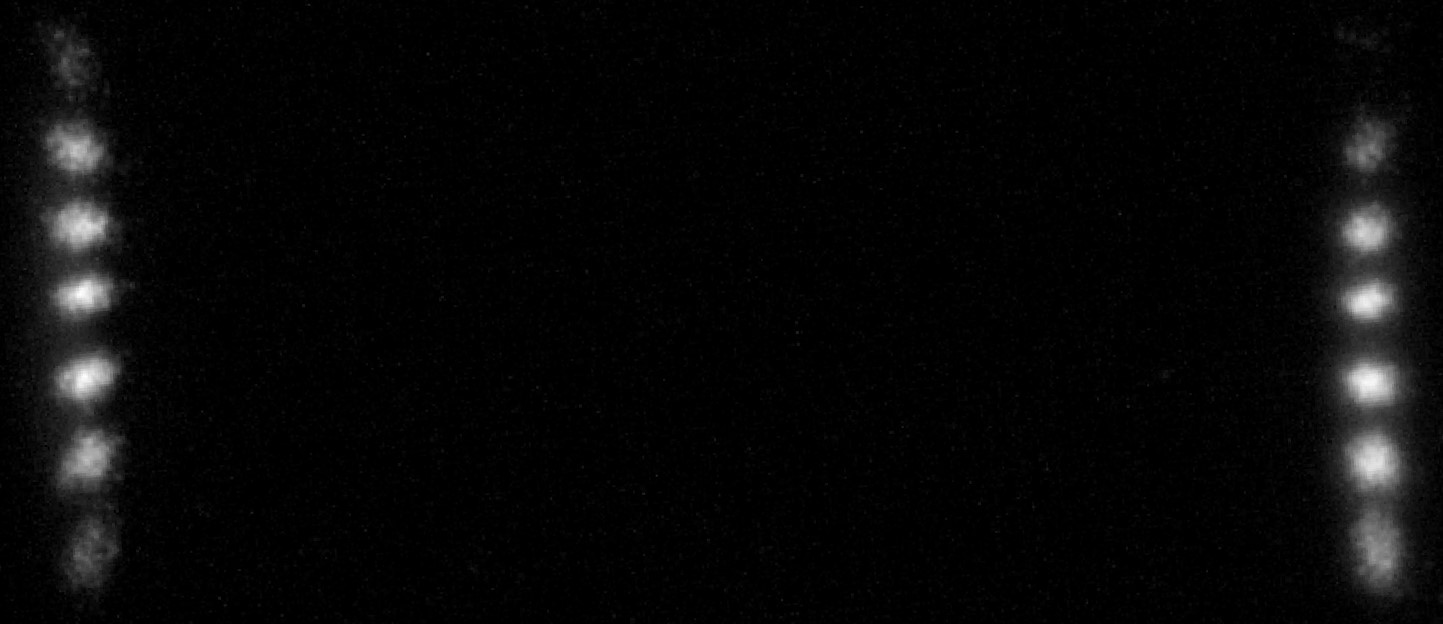
\includegraphics[width=0.5\linewidth]{part2/Figs/example_calibration.jpeg}
    \caption{An example of an image used to calibration the timing of the streaked pepperpots.}
    % Set 9 2017.06.11
    \label{figure:example_calibration}
\end{figure}

\subsection{Pepperpots}
There were a number of iterations on the precise configuration of the one- and two-dimensional pepperpots used in these experiments.
There are a number of considerations when designing pepperpot masks;
\begin{itemize}
    \item{\emph{Aperture size:} Smaller apertures provide a better resolution to the emittance measurement but reduce the signal as fewer particles pass through the hole.
    Aperture size affects the size of the beamlets on the detector, which impacts the overlap of beamlets on the detector, as the beamlets are a convolution of the aperture and the beam divergence. Smaller apertures also allow for a smaller aperture spacing as when the aperture diameter and aperture spacing are similar the pepperpot can become fragile.}
    \item{\emph{Aperture spacing:} Aperture spacing, also known as pitch, determines how well the full beam is sampled.
    Smaller pitch allows for better sampling of the full beam however pitch should be large enough that the beamlet overlap on the detector is manageable.
    If the pitch is too small then the pepperpot can also become fragile.}
    \item{\emph{Extent:} Ideally a the total extend of the pepperpot should be much larger than the largest beam for a particular apparatus.
    Unfortunately, due to the mounting arrangement of the Melbourne \gls{caeis}, the size of samples was limited to \unit[3]{mm} diameter and only a \unit[2]{mm} diameter portion of the sample was accessible to the beam. A view of the sample holder without the `lid' is shown in Figure~\ref{figure:sample_holder_pepperpots}.}
\end{itemize}

A number of restrictions aided the selection of parameters for the pepperpots used, the maximum pepperpot extent and need to focus the beam to the pepperpot size to maximise flux dictated the approximate size of the beamlets on the detector and thus the lowest feasibly pitch in order to minimise the overlap of beamlets on the detector.
The pepperpots were cut\footnote{The pepperpots were cut using a Oxford Laser Systems Alpha 532 laser micromachining system.} from \unit[25]{$\mu m$} thick copper pinholes\footnote{Gilder Grids GA50-C3, \unit[50]{$\mu m$} aperture.} with \unit[50]{$\mu m$} diameter holes cut in the centre.
The central pinholes were used as the central aperture for the pepperpot arrays and since \unit[50]{$\mu m$} apertures provide adequate flux the rest of the apertures were also cut to the same diameter to simplify analysis while providing acceptable measurement resolution.
A pitch of \unit[200]{$\mu m$} was chosen to provide acceptable sampling of the beam while minimising the overlap of beamlets on the detector.
Given the \unit[2]{mm} diameter available this pitch allowed for one dimensional pepperpots with 7 apertures and two dimensional pepperpots with 7$\times$7 apertures.
The pepperpots used are shown in Figures~\ref{figure:pepperpot_mask} and \ref{figure:1d_pepperpot}.

\begin{figure}
    \center
    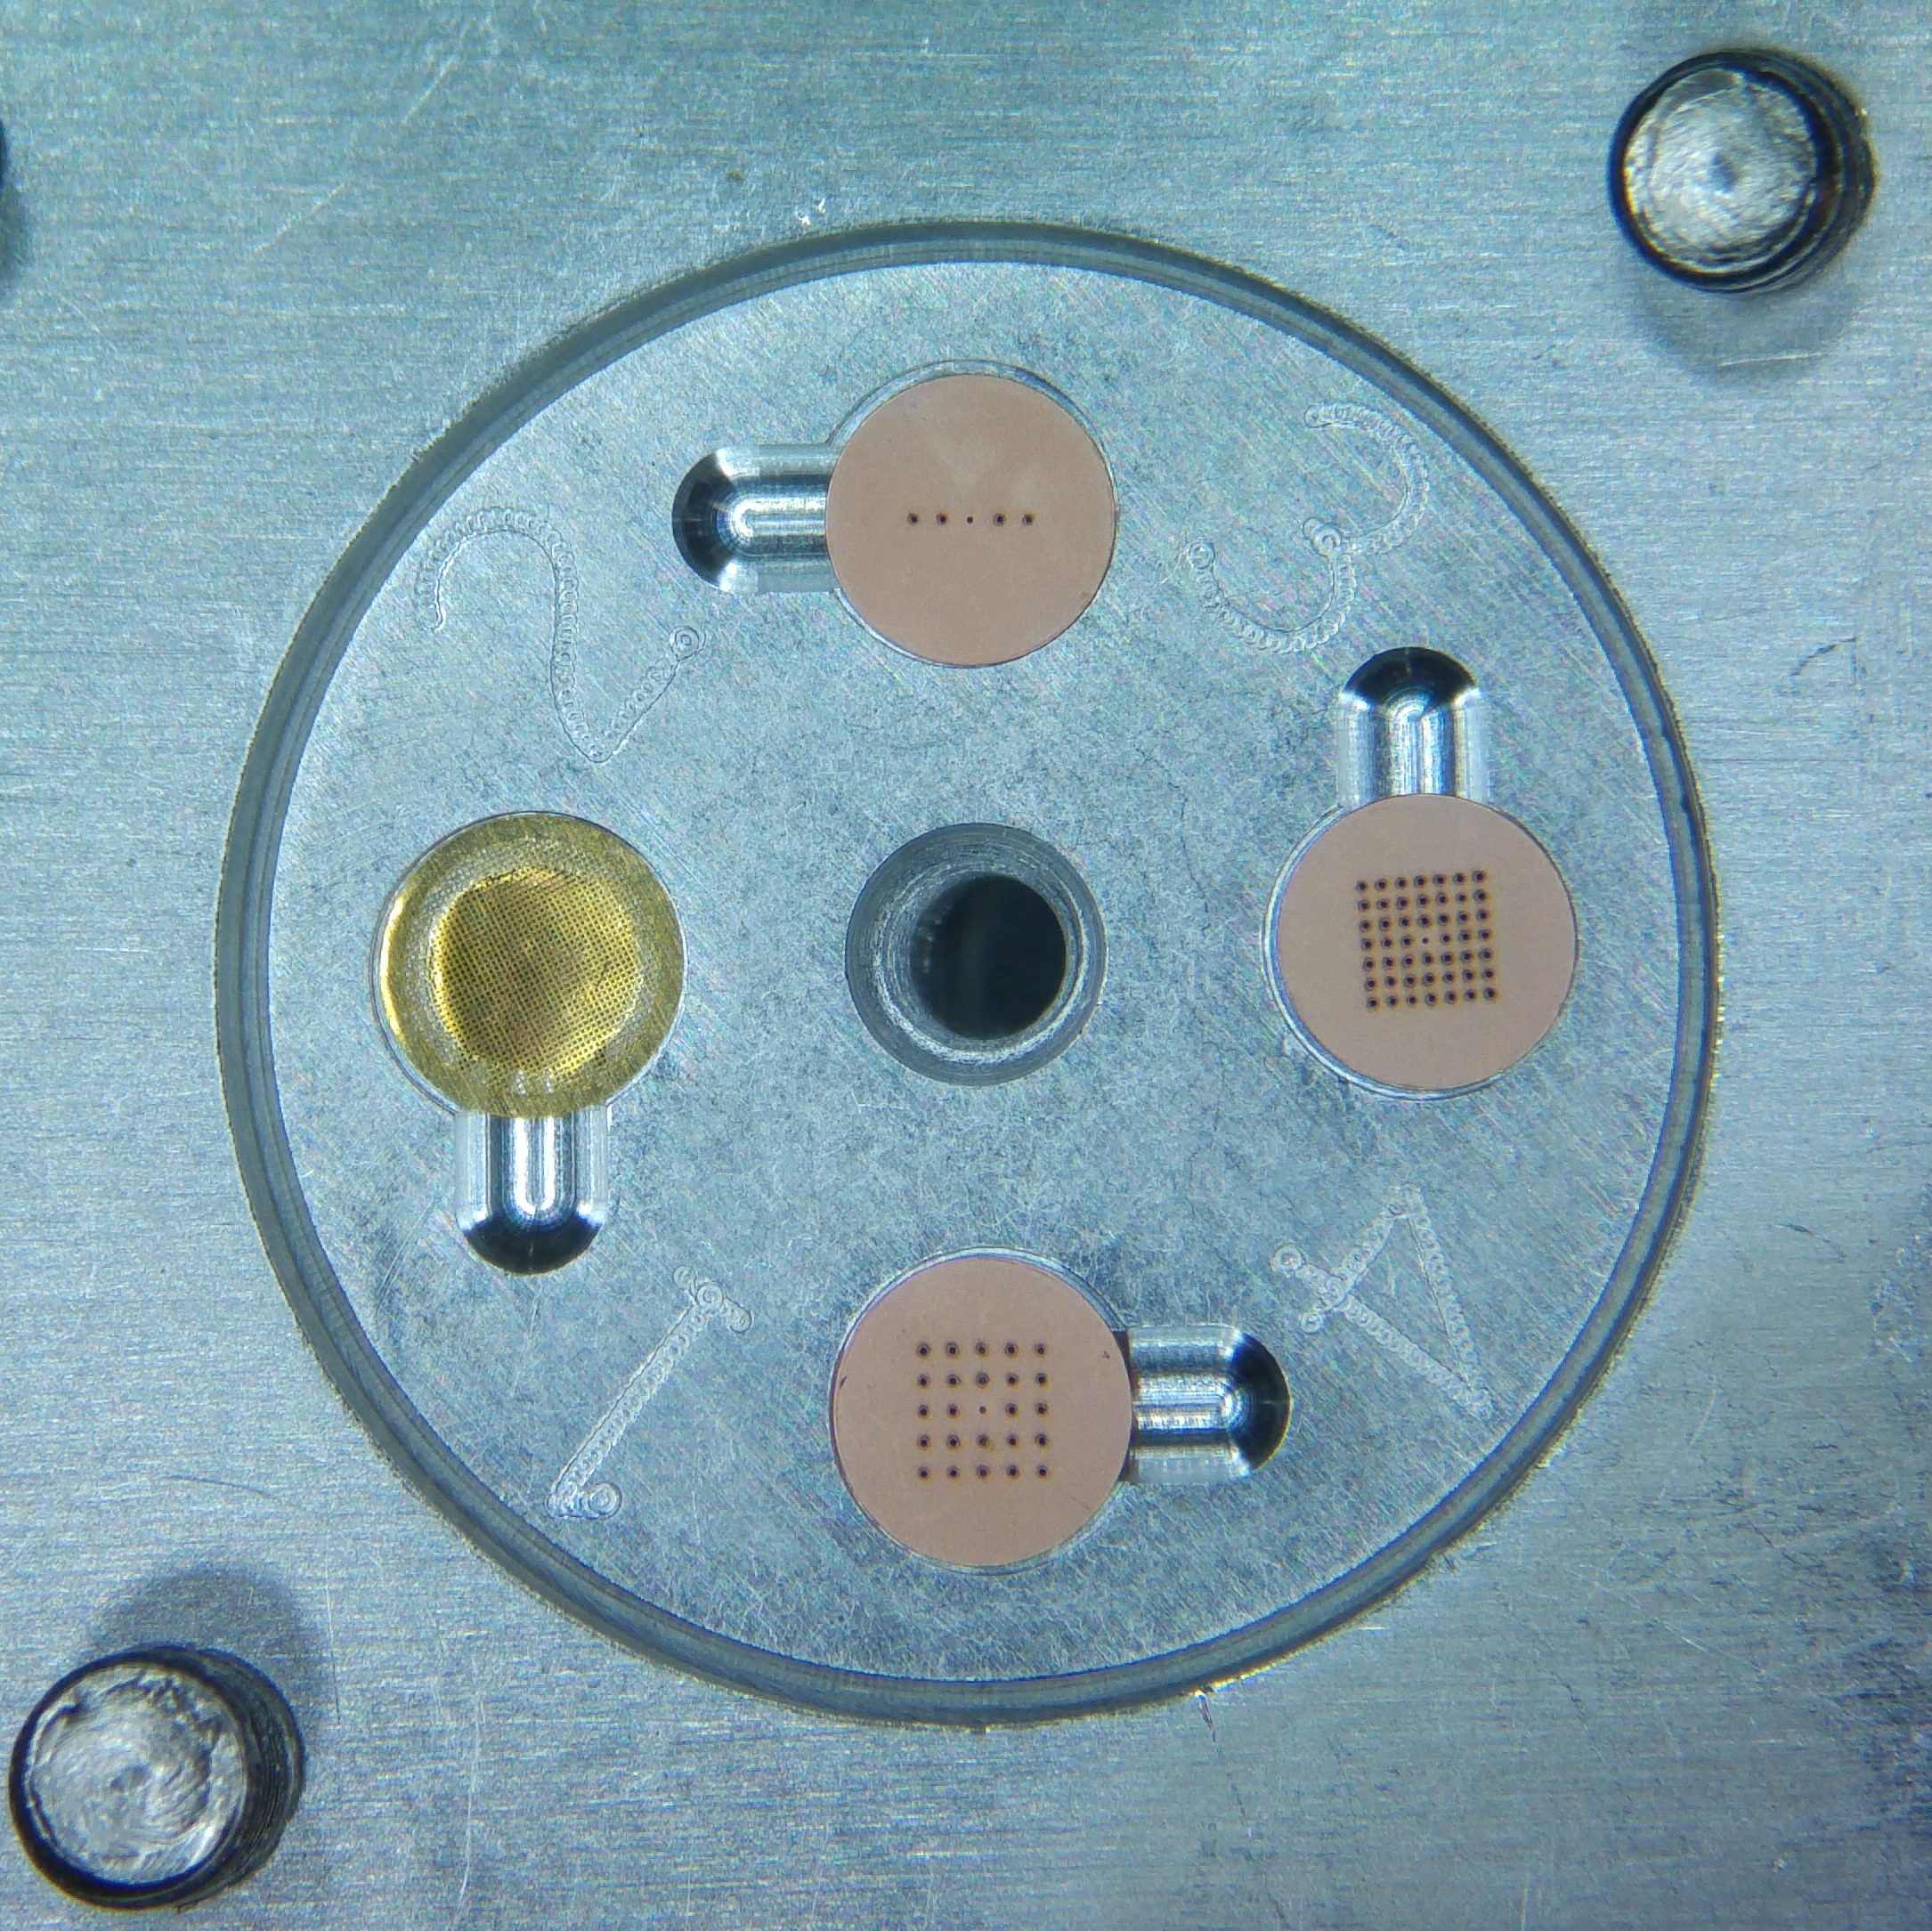
\includegraphics[width=0.49\linewidth]{part2/Figs/sample_holder.jpg}
    \caption{One of two sample holders that are used to load up to eight samples into the vacuum system. Clockwise from the top: five \unit[50]{$\mu m$} apertures with \unit[300]{$\mu m$} pitch, 7 by 7 pepperpot of \unit[50]{$\mu m$} apertures with \unit[200]{$\mu m$} pitch, 5 by 5 pepperpot of \unit[50]{$\mu m$} apertures with \unit[300]{$\mu m$} pitch, thin gold sample. Each sample is \unit[3]{mm} in diameter. A `lid' with appropriate apertures is placed over the samples to hold them in place.}
    \label{figure:sample_holder_pepperpots}
\end{figure}

\subsection{Laser Parameters}
Two of the lasers essential to the functioning are the `excitation' and `ionisation' lasers, see Section~\ref{section:two_stage_ionisation}, a CW red and pulsed blue laser respectively.
These lasers have a number of parameters that affect the emittance measurements.

\subsubsection{Excitation Laser}
The excitation laser was a \unit[780]{nm} laser, frequency locked to the Rb85 D2 F=3 to F=4 transition, which excites ground state atoms in the \gls{mot} to prepare the atoms for ionisation.
The spatial profile of this laser is highly controllable with a \gls{slm} allowing for arbitrary profiles to be mapped to the electron or ion bunch~\cite{mcculloch_arbitrarily_2011}.
The highest flux is possible by simply saturating the \gls{mot} however control over the electron beam profile and size is usually desirable.
One commonly used and simple distribution is a flat-top distribution as it can provide even electron intensity across the sample under examination however electron beams generated from electrons with high excess energy are unable to maintain the distribution, see Figure~\ref{figure:flat_top}.

\begin{figure}
    \center
    %% Creator: Matplotlib, PGF backend
%%
%% To include the figure in your LaTeX document, write
%%   \input{<filename>.pgf}
%%
%% Make sure the required packages are loaded in your preamble
%%   \usepackage{pgf}
%%
%% Figures using additional raster images can only be included by \input if
%% they are in the same directory as the main LaTeX file. For loading figures
%% from other directories you can use the `import` package
%%   \usepackage{import}
%% and then include the figures with
%%   \import{<path to file>}{<filename>.pgf}
%%
%% Matplotlib used the following preamble
%%
\begingroup%
\makeatletter%
\begin{pgfpicture}%
\pgfpathrectangle{\pgfpointorigin}{\pgfqpoint{5.424500in}{3.977967in}}%
\pgfusepath{use as bounding box, clip}%
\begin{pgfscope}%
\pgfsetbuttcap%
\pgfsetmiterjoin%
\definecolor{currentfill}{rgb}{1.000000,1.000000,1.000000}%
\pgfsetfillcolor{currentfill}%
\pgfsetlinewidth{0.000000pt}%
\definecolor{currentstroke}{rgb}{1.000000,1.000000,1.000000}%
\pgfsetstrokecolor{currentstroke}%
\pgfsetdash{}{0pt}%
\pgfpathmoveto{\pgfqpoint{0.000000in}{0.000000in}}%
\pgfpathlineto{\pgfqpoint{5.424500in}{0.000000in}}%
\pgfpathlineto{\pgfqpoint{5.424500in}{3.977967in}}%
\pgfpathlineto{\pgfqpoint{0.000000in}{3.977967in}}%
\pgfpathclose%
\pgfusepath{fill}%
\end{pgfscope}%
\begin{pgfscope}%
\pgfsetbuttcap%
\pgfsetmiterjoin%
\definecolor{currentfill}{rgb}{1.000000,1.000000,1.000000}%
\pgfsetfillcolor{currentfill}%
\pgfsetlinewidth{0.000000pt}%
\definecolor{currentstroke}{rgb}{0.000000,0.000000,0.000000}%
\pgfsetstrokecolor{currentstroke}%
\pgfsetstrokeopacity{0.000000}%
\pgfsetdash{}{0pt}%
\pgfpathmoveto{\pgfqpoint{0.396944in}{2.104261in}}%
\pgfpathlineto{\pgfqpoint{2.017796in}{2.104261in}}%
\pgfpathlineto{\pgfqpoint{2.017796in}{3.593522in}}%
\pgfpathlineto{\pgfqpoint{0.396944in}{3.593522in}}%
\pgfpathclose%
\pgfusepath{fill}%
\end{pgfscope}%
\begin{pgfscope}%
\pgfpathrectangle{\pgfqpoint{0.396944in}{2.104261in}}{\pgfqpoint{1.620852in}{1.489261in}} %
\pgfusepath{clip}%
\pgftext[at=\pgfqpoint{0.396944in}{2.104261in},left,bottom]{\pgfimage[interpolate=true,width=1.630000in,height=1.500000in]{flattops_emittance-img0.png}}%
\end{pgfscope}%
\begin{pgfscope}%
\pgfpathrectangle{\pgfqpoint{0.396944in}{2.104261in}}{\pgfqpoint{1.620852in}{1.489261in}} %
\pgfusepath{clip}%
\pgfsetbuttcap%
\pgfsetroundjoin%
\pgfsetlinewidth{1.003750pt}%
\definecolor{currentstroke}{rgb}{1.000000,1.000000,1.000000}%
\pgfsetstrokecolor{currentstroke}%
\pgfsetdash{{6.000000pt}{6.000000pt}}{0.000000pt}%
\pgfpathmoveto{\pgfqpoint{0.396944in}{2.846410in}}%
\pgfpathlineto{\pgfqpoint{2.017796in}{2.846410in}}%
\pgfusepath{stroke}%
\end{pgfscope}%
\begin{pgfscope}%
\pgfsetrectcap%
\pgfsetmiterjoin%
\pgfsetlinewidth{1.003750pt}%
\definecolor{currentstroke}{rgb}{0.000000,0.000000,0.000000}%
\pgfsetstrokecolor{currentstroke}%
\pgfsetdash{}{0pt}%
\pgfpathmoveto{\pgfqpoint{0.396944in}{2.104261in}}%
\pgfpathlineto{\pgfqpoint{0.396944in}{3.593522in}}%
\pgfusepath{stroke}%
\end{pgfscope}%
\begin{pgfscope}%
\pgfsetrectcap%
\pgfsetmiterjoin%
\pgfsetlinewidth{1.003750pt}%
\definecolor{currentstroke}{rgb}{0.000000,0.000000,0.000000}%
\pgfsetstrokecolor{currentstroke}%
\pgfsetdash{}{0pt}%
\pgfpathmoveto{\pgfqpoint{0.396944in}{2.104261in}}%
\pgfpathlineto{\pgfqpoint{2.017796in}{2.104261in}}%
\pgfusepath{stroke}%
\end{pgfscope}%
\begin{pgfscope}%
\pgfsetrectcap%
\pgfsetmiterjoin%
\pgfsetlinewidth{1.003750pt}%
\definecolor{currentstroke}{rgb}{0.000000,0.000000,0.000000}%
\pgfsetstrokecolor{currentstroke}%
\pgfsetdash{}{0pt}%
\pgfpathmoveto{\pgfqpoint{0.396944in}{3.593522in}}%
\pgfpathlineto{\pgfqpoint{2.017796in}{3.593522in}}%
\pgfusepath{stroke}%
\end{pgfscope}%
\begin{pgfscope}%
\pgfsetrectcap%
\pgfsetmiterjoin%
\pgfsetlinewidth{1.003750pt}%
\definecolor{currentstroke}{rgb}{0.000000,0.000000,0.000000}%
\pgfsetstrokecolor{currentstroke}%
\pgfsetdash{}{0pt}%
\pgfpathmoveto{\pgfqpoint{2.017796in}{2.104261in}}%
\pgfpathlineto{\pgfqpoint{2.017796in}{3.593522in}}%
\pgfusepath{stroke}%
\end{pgfscope}%
\begin{pgfscope}%
\pgftext[x=1.207370in,y=3.662967in,,base]{\rmfamily\fontsize{13.200000}{15.840000}\selectfont -42.0\(\displaystyle \,\)meV}%
\end{pgfscope}%
\begin{pgfscope}%
\pgfsetbuttcap%
\pgfsetmiterjoin%
\definecolor{currentfill}{rgb}{1.000000,1.000000,1.000000}%
\pgfsetfillcolor{currentfill}%
\pgfsetlinewidth{0.000000pt}%
\definecolor{currentstroke}{rgb}{0.000000,0.000000,0.000000}%
\pgfsetstrokecolor{currentstroke}%
\pgfsetstrokeopacity{0.000000}%
\pgfsetdash{}{0pt}%
\pgfpathmoveto{\pgfqpoint{0.396944in}{0.615000in}}%
\pgfpathlineto{\pgfqpoint{2.017796in}{0.615000in}}%
\pgfpathlineto{\pgfqpoint{2.017796in}{2.104261in}}%
\pgfpathlineto{\pgfqpoint{0.396944in}{2.104261in}}%
\pgfpathclose%
\pgfusepath{fill}%
\end{pgfscope}%
\begin{pgfscope}%
\pgfpathrectangle{\pgfqpoint{0.396944in}{0.615000in}}{\pgfqpoint{1.620852in}{1.489261in}} %
\pgfusepath{clip}%
\pgfsetbuttcap%
\pgfsetroundjoin%
\pgfsetlinewidth{1.003750pt}%
\definecolor{currentstroke}{rgb}{1.000000,0.000000,0.000000}%
\pgfsetstrokecolor{currentstroke}%
\pgfsetdash{{1.000000pt}{3.000000pt}}{0.000000pt}%
\pgfpathmoveto{\pgfqpoint{0.396944in}{0.624506in}}%
\pgfpathlineto{\pgfqpoint{0.402347in}{0.617183in}}%
\pgfpathlineto{\pgfqpoint{0.407750in}{0.615000in}}%
\pgfpathlineto{\pgfqpoint{0.413153in}{0.615830in}}%
\pgfpathlineto{\pgfqpoint{0.418556in}{0.618413in}}%
\pgfpathlineto{\pgfqpoint{0.434764in}{0.633164in}}%
\pgfpathlineto{\pgfqpoint{0.445570in}{0.631717in}}%
\pgfpathlineto{\pgfqpoint{0.450973in}{0.629860in}}%
\pgfpathlineto{\pgfqpoint{0.456376in}{0.633103in}}%
\pgfpathlineto{\pgfqpoint{0.461779in}{0.641380in}}%
\pgfpathlineto{\pgfqpoint{0.472584in}{0.653406in}}%
\pgfpathlineto{\pgfqpoint{0.477987in}{0.663637in}}%
\pgfpathlineto{\pgfqpoint{0.488793in}{0.674176in}}%
\pgfpathlineto{\pgfqpoint{0.494196in}{0.674855in}}%
\pgfpathlineto{\pgfqpoint{0.499598in}{0.680154in}}%
\pgfpathlineto{\pgfqpoint{0.505001in}{0.682156in}}%
\pgfpathlineto{\pgfqpoint{0.510404in}{0.692276in}}%
\pgfpathlineto{\pgfqpoint{0.515807in}{0.698970in}}%
\pgfpathlineto{\pgfqpoint{0.521210in}{0.701174in}}%
\pgfpathlineto{\pgfqpoint{0.532015in}{0.725330in}}%
\pgfpathlineto{\pgfqpoint{0.542821in}{0.753712in}}%
\pgfpathlineto{\pgfqpoint{0.548224in}{0.764961in}}%
\pgfpathlineto{\pgfqpoint{0.559030in}{0.773106in}}%
\pgfpathlineto{\pgfqpoint{0.564432in}{0.782553in}}%
\pgfpathlineto{\pgfqpoint{0.569835in}{0.795326in}}%
\pgfpathlineto{\pgfqpoint{0.580641in}{0.828780in}}%
\pgfpathlineto{\pgfqpoint{0.591447in}{0.846073in}}%
\pgfpathlineto{\pgfqpoint{0.596850in}{0.848364in}}%
\pgfpathlineto{\pgfqpoint{0.613058in}{0.908456in}}%
\pgfpathlineto{\pgfqpoint{0.623864in}{0.937368in}}%
\pgfpathlineto{\pgfqpoint{0.629267in}{0.949366in}}%
\pgfpathlineto{\pgfqpoint{0.640072in}{0.984131in}}%
\pgfpathlineto{\pgfqpoint{0.645475in}{0.996817in}}%
\pgfpathlineto{\pgfqpoint{0.650878in}{1.015002in}}%
\pgfpathlineto{\pgfqpoint{0.656281in}{1.023664in}}%
\pgfpathlineto{\pgfqpoint{0.661684in}{1.037305in}}%
\pgfpathlineto{\pgfqpoint{0.667086in}{1.043856in}}%
\pgfpathlineto{\pgfqpoint{0.683295in}{1.095942in}}%
\pgfpathlineto{\pgfqpoint{0.688698in}{1.110675in}}%
\pgfpathlineto{\pgfqpoint{0.694101in}{1.133854in}}%
\pgfpathlineto{\pgfqpoint{0.699503in}{1.144489in}}%
\pgfpathlineto{\pgfqpoint{0.704906in}{1.161049in}}%
\pgfpathlineto{\pgfqpoint{0.710309in}{1.186676in}}%
\pgfpathlineto{\pgfqpoint{0.715712in}{1.198221in}}%
\pgfpathlineto{\pgfqpoint{0.726518in}{1.217748in}}%
\pgfpathlineto{\pgfqpoint{0.731920in}{1.247198in}}%
\pgfpathlineto{\pgfqpoint{0.742726in}{1.291361in}}%
\pgfpathlineto{\pgfqpoint{0.753532in}{1.329699in}}%
\pgfpathlineto{\pgfqpoint{0.758935in}{1.330222in}}%
\pgfpathlineto{\pgfqpoint{0.764338in}{1.337509in}}%
\pgfpathlineto{\pgfqpoint{0.769740in}{1.352766in}}%
\pgfpathlineto{\pgfqpoint{0.775143in}{1.377587in}}%
\pgfpathlineto{\pgfqpoint{0.780546in}{1.395487in}}%
\pgfpathlineto{\pgfqpoint{0.785949in}{1.425367in}}%
\pgfpathlineto{\pgfqpoint{0.791352in}{1.447276in}}%
\pgfpathlineto{\pgfqpoint{0.796755in}{1.454341in}}%
\pgfpathlineto{\pgfqpoint{0.802157in}{1.456747in}}%
\pgfpathlineto{\pgfqpoint{0.807560in}{1.466169in}}%
\pgfpathlineto{\pgfqpoint{0.812963in}{1.478067in}}%
\pgfpathlineto{\pgfqpoint{0.818366in}{1.500692in}}%
\pgfpathlineto{\pgfqpoint{0.823769in}{1.506510in}}%
\pgfpathlineto{\pgfqpoint{0.834574in}{1.500069in}}%
\pgfpathlineto{\pgfqpoint{0.845380in}{1.517184in}}%
\pgfpathlineto{\pgfqpoint{0.861589in}{1.609881in}}%
\pgfpathlineto{\pgfqpoint{0.872394in}{1.625364in}}%
\pgfpathlineto{\pgfqpoint{0.877797in}{1.641911in}}%
\pgfpathlineto{\pgfqpoint{0.883200in}{1.676034in}}%
\pgfpathlineto{\pgfqpoint{0.888603in}{1.696906in}}%
\pgfpathlineto{\pgfqpoint{0.904811in}{1.705828in}}%
\pgfpathlineto{\pgfqpoint{0.910214in}{1.698244in}}%
\pgfpathlineto{\pgfqpoint{0.915617in}{1.704252in}}%
\pgfpathlineto{\pgfqpoint{0.921020in}{1.717012in}}%
\pgfpathlineto{\pgfqpoint{0.926423in}{1.746840in}}%
\pgfpathlineto{\pgfqpoint{0.931826in}{1.743679in}}%
\pgfpathlineto{\pgfqpoint{0.937228in}{1.742522in}}%
\pgfpathlineto{\pgfqpoint{0.942631in}{1.723305in}}%
\pgfpathlineto{\pgfqpoint{0.948034in}{1.711510in}}%
\pgfpathlineto{\pgfqpoint{0.953437in}{1.731151in}}%
\pgfpathlineto{\pgfqpoint{0.964243in}{1.758237in}}%
\pgfpathlineto{\pgfqpoint{0.969645in}{1.770696in}}%
\pgfpathlineto{\pgfqpoint{0.975048in}{1.763072in}}%
\pgfpathlineto{\pgfqpoint{0.980451in}{1.743022in}}%
\pgfpathlineto{\pgfqpoint{0.985854in}{1.741979in}}%
\pgfpathlineto{\pgfqpoint{0.991257in}{1.768678in}}%
\pgfpathlineto{\pgfqpoint{1.002062in}{1.804722in}}%
\pgfpathlineto{\pgfqpoint{1.012868in}{1.800859in}}%
\pgfpathlineto{\pgfqpoint{1.018271in}{1.804120in}}%
\pgfpathlineto{\pgfqpoint{1.023674in}{1.809490in}}%
\pgfpathlineto{\pgfqpoint{1.029077in}{1.830170in}}%
\pgfpathlineto{\pgfqpoint{1.034480in}{1.855304in}}%
\pgfpathlineto{\pgfqpoint{1.039882in}{1.850514in}}%
\pgfpathlineto{\pgfqpoint{1.045285in}{1.849056in}}%
\pgfpathlineto{\pgfqpoint{1.050688in}{1.845176in}}%
\pgfpathlineto{\pgfqpoint{1.056091in}{1.847910in}}%
\pgfpathlineto{\pgfqpoint{1.066897in}{1.918792in}}%
\pgfpathlineto{\pgfqpoint{1.072299in}{1.936413in}}%
\pgfpathlineto{\pgfqpoint{1.077702in}{1.942640in}}%
\pgfpathlineto{\pgfqpoint{1.083105in}{1.919165in}}%
\pgfpathlineto{\pgfqpoint{1.088508in}{1.929888in}}%
\pgfpathlineto{\pgfqpoint{1.093911in}{1.949997in}}%
\pgfpathlineto{\pgfqpoint{1.099314in}{1.984919in}}%
\pgfpathlineto{\pgfqpoint{1.104716in}{1.997039in}}%
\pgfpathlineto{\pgfqpoint{1.110119in}{1.985391in}}%
\pgfpathlineto{\pgfqpoint{1.115522in}{1.979564in}}%
\pgfpathlineto{\pgfqpoint{1.120925in}{1.993797in}}%
\pgfpathlineto{\pgfqpoint{1.131731in}{2.014487in}}%
\pgfpathlineto{\pgfqpoint{1.137133in}{2.028705in}}%
\pgfpathlineto{\pgfqpoint{1.147939in}{2.005485in}}%
\pgfpathlineto{\pgfqpoint{1.153342in}{1.978272in}}%
\pgfpathlineto{\pgfqpoint{1.158745in}{1.991513in}}%
\pgfpathlineto{\pgfqpoint{1.164148in}{1.999734in}}%
\pgfpathlineto{\pgfqpoint{1.169550in}{2.021193in}}%
\pgfpathlineto{\pgfqpoint{1.174953in}{2.033344in}}%
\pgfpathlineto{\pgfqpoint{1.180356in}{2.021453in}}%
\pgfpathlineto{\pgfqpoint{1.191162in}{1.975564in}}%
\pgfpathlineto{\pgfqpoint{1.196565in}{1.979900in}}%
\pgfpathlineto{\pgfqpoint{1.201968in}{1.996861in}}%
\pgfpathlineto{\pgfqpoint{1.207370in}{2.017661in}}%
\pgfpathlineto{\pgfqpoint{1.218176in}{2.001975in}}%
\pgfpathlineto{\pgfqpoint{1.228982in}{1.963851in}}%
\pgfpathlineto{\pgfqpoint{1.234385in}{1.983969in}}%
\pgfpathlineto{\pgfqpoint{1.239787in}{2.015341in}}%
\pgfpathlineto{\pgfqpoint{1.245190in}{2.015105in}}%
\pgfpathlineto{\pgfqpoint{1.250593in}{1.986095in}}%
\pgfpathlineto{\pgfqpoint{1.261399in}{1.953630in}}%
\pgfpathlineto{\pgfqpoint{1.266802in}{1.949386in}}%
\pgfpathlineto{\pgfqpoint{1.272204in}{1.966186in}}%
\pgfpathlineto{\pgfqpoint{1.277607in}{1.958593in}}%
\pgfpathlineto{\pgfqpoint{1.283010in}{1.955774in}}%
\pgfpathlineto{\pgfqpoint{1.293816in}{1.916153in}}%
\pgfpathlineto{\pgfqpoint{1.299219in}{1.912828in}}%
\pgfpathlineto{\pgfqpoint{1.304621in}{1.916281in}}%
\pgfpathlineto{\pgfqpoint{1.310024in}{1.929046in}}%
\pgfpathlineto{\pgfqpoint{1.320830in}{1.911792in}}%
\pgfpathlineto{\pgfqpoint{1.331636in}{1.881268in}}%
\pgfpathlineto{\pgfqpoint{1.337039in}{1.890023in}}%
\pgfpathlineto{\pgfqpoint{1.342441in}{1.905559in}}%
\pgfpathlineto{\pgfqpoint{1.347844in}{1.914307in}}%
\pgfpathlineto{\pgfqpoint{1.358650in}{1.901259in}}%
\pgfpathlineto{\pgfqpoint{1.364053in}{1.879160in}}%
\pgfpathlineto{\pgfqpoint{1.369456in}{1.868038in}}%
\pgfpathlineto{\pgfqpoint{1.374858in}{1.869194in}}%
\pgfpathlineto{\pgfqpoint{1.380261in}{1.891658in}}%
\pgfpathlineto{\pgfqpoint{1.385664in}{1.898922in}}%
\pgfpathlineto{\pgfqpoint{1.391067in}{1.884713in}}%
\pgfpathlineto{\pgfqpoint{1.396470in}{1.850157in}}%
\pgfpathlineto{\pgfqpoint{1.401873in}{1.825040in}}%
\pgfpathlineto{\pgfqpoint{1.407275in}{1.821226in}}%
\pgfpathlineto{\pgfqpoint{1.412678in}{1.826164in}}%
\pgfpathlineto{\pgfqpoint{1.418081in}{1.814499in}}%
\pgfpathlineto{\pgfqpoint{1.423484in}{1.806746in}}%
\pgfpathlineto{\pgfqpoint{1.428887in}{1.786458in}}%
\pgfpathlineto{\pgfqpoint{1.439692in}{1.717497in}}%
\pgfpathlineto{\pgfqpoint{1.445095in}{1.736045in}}%
\pgfpathlineto{\pgfqpoint{1.455901in}{1.783806in}}%
\pgfpathlineto{\pgfqpoint{1.461304in}{1.778362in}}%
\pgfpathlineto{\pgfqpoint{1.466707in}{1.759812in}}%
\pgfpathlineto{\pgfqpoint{1.472110in}{1.725997in}}%
\pgfpathlineto{\pgfqpoint{1.477512in}{1.745386in}}%
\pgfpathlineto{\pgfqpoint{1.482915in}{1.737790in}}%
\pgfpathlineto{\pgfqpoint{1.488318in}{1.726730in}}%
\pgfpathlineto{\pgfqpoint{1.499124in}{1.692137in}}%
\pgfpathlineto{\pgfqpoint{1.504527in}{1.657320in}}%
\pgfpathlineto{\pgfqpoint{1.515332in}{1.611988in}}%
\pgfpathlineto{\pgfqpoint{1.520735in}{1.620910in}}%
\pgfpathlineto{\pgfqpoint{1.526138in}{1.609485in}}%
\pgfpathlineto{\pgfqpoint{1.531541in}{1.592182in}}%
\pgfpathlineto{\pgfqpoint{1.536944in}{1.565616in}}%
\pgfpathlineto{\pgfqpoint{1.542346in}{1.530017in}}%
\pgfpathlineto{\pgfqpoint{1.547749in}{1.513145in}}%
\pgfpathlineto{\pgfqpoint{1.553152in}{1.506941in}}%
\pgfpathlineto{\pgfqpoint{1.563958in}{1.488595in}}%
\pgfpathlineto{\pgfqpoint{1.569361in}{1.490645in}}%
\pgfpathlineto{\pgfqpoint{1.580166in}{1.446096in}}%
\pgfpathlineto{\pgfqpoint{1.585569in}{1.435569in}}%
\pgfpathlineto{\pgfqpoint{1.590972in}{1.434589in}}%
\pgfpathlineto{\pgfqpoint{1.596375in}{1.426068in}}%
\pgfpathlineto{\pgfqpoint{1.601778in}{1.413680in}}%
\pgfpathlineto{\pgfqpoint{1.607180in}{1.389409in}}%
\pgfpathlineto{\pgfqpoint{1.617986in}{1.325803in}}%
\pgfpathlineto{\pgfqpoint{1.623389in}{1.309119in}}%
\pgfpathlineto{\pgfqpoint{1.645000in}{1.228860in}}%
\pgfpathlineto{\pgfqpoint{1.650403in}{1.198382in}}%
\pgfpathlineto{\pgfqpoint{1.655806in}{1.174633in}}%
\pgfpathlineto{\pgfqpoint{1.661209in}{1.160604in}}%
\pgfpathlineto{\pgfqpoint{1.672015in}{1.120440in}}%
\pgfpathlineto{\pgfqpoint{1.677417in}{1.107922in}}%
\pgfpathlineto{\pgfqpoint{1.682820in}{1.089267in}}%
\pgfpathlineto{\pgfqpoint{1.688223in}{1.094514in}}%
\pgfpathlineto{\pgfqpoint{1.693626in}{1.083771in}}%
\pgfpathlineto{\pgfqpoint{1.699029in}{1.057427in}}%
\pgfpathlineto{\pgfqpoint{1.709834in}{0.999439in}}%
\pgfpathlineto{\pgfqpoint{1.715237in}{0.990971in}}%
\pgfpathlineto{\pgfqpoint{1.720640in}{0.976461in}}%
\pgfpathlineto{\pgfqpoint{1.731446in}{0.959648in}}%
\pgfpathlineto{\pgfqpoint{1.747654in}{0.905056in}}%
\pgfpathlineto{\pgfqpoint{1.758460in}{0.860632in}}%
\pgfpathlineto{\pgfqpoint{1.763863in}{0.859552in}}%
\pgfpathlineto{\pgfqpoint{1.769266in}{0.843635in}}%
\pgfpathlineto{\pgfqpoint{1.785474in}{0.806525in}}%
\pgfpathlineto{\pgfqpoint{1.790877in}{0.793159in}}%
\pgfpathlineto{\pgfqpoint{1.801683in}{0.779348in}}%
\pgfpathlineto{\pgfqpoint{1.817891in}{0.740778in}}%
\pgfpathlineto{\pgfqpoint{1.823294in}{0.736172in}}%
\pgfpathlineto{\pgfqpoint{1.828697in}{0.735359in}}%
\pgfpathlineto{\pgfqpoint{1.839503in}{0.738763in}}%
\pgfpathlineto{\pgfqpoint{1.844905in}{0.729006in}}%
\pgfpathlineto{\pgfqpoint{1.850308in}{0.725054in}}%
\pgfpathlineto{\pgfqpoint{1.861114in}{0.727545in}}%
\pgfpathlineto{\pgfqpoint{1.866517in}{0.726100in}}%
\pgfpathlineto{\pgfqpoint{1.871920in}{0.723010in}}%
\pgfpathlineto{\pgfqpoint{1.877322in}{0.713266in}}%
\pgfpathlineto{\pgfqpoint{1.882725in}{0.706297in}}%
\pgfpathlineto{\pgfqpoint{1.888128in}{0.694800in}}%
\pgfpathlineto{\pgfqpoint{1.893531in}{0.686121in}}%
\pgfpathlineto{\pgfqpoint{1.898934in}{0.683309in}}%
\pgfpathlineto{\pgfqpoint{1.904337in}{0.683408in}}%
\pgfpathlineto{\pgfqpoint{1.915142in}{0.673374in}}%
\pgfpathlineto{\pgfqpoint{1.920545in}{0.670289in}}%
\pgfpathlineto{\pgfqpoint{1.925948in}{0.664697in}}%
\pgfpathlineto{\pgfqpoint{1.931351in}{0.664232in}}%
\pgfpathlineto{\pgfqpoint{1.936754in}{0.670154in}}%
\pgfpathlineto{\pgfqpoint{1.942157in}{0.678123in}}%
\pgfpathlineto{\pgfqpoint{1.947559in}{0.681880in}}%
\pgfpathlineto{\pgfqpoint{1.952962in}{0.679534in}}%
\pgfpathlineto{\pgfqpoint{1.958365in}{0.674227in}}%
\pgfpathlineto{\pgfqpoint{1.963768in}{0.666296in}}%
\pgfpathlineto{\pgfqpoint{1.969171in}{0.673768in}}%
\pgfpathlineto{\pgfqpoint{1.974574in}{0.684694in}}%
\pgfpathlineto{\pgfqpoint{1.979976in}{0.685555in}}%
\pgfpathlineto{\pgfqpoint{1.985379in}{0.681985in}}%
\pgfpathlineto{\pgfqpoint{1.990782in}{0.672626in}}%
\pgfpathlineto{\pgfqpoint{1.996185in}{0.666338in}}%
\pgfpathlineto{\pgfqpoint{2.012393in}{0.665880in}}%
\pgfpathlineto{\pgfqpoint{2.012393in}{0.665880in}}%
\pgfusepath{stroke}%
\end{pgfscope}%
\begin{pgfscope}%
\pgfpathrectangle{\pgfqpoint{0.396944in}{0.615000in}}{\pgfqpoint{1.620852in}{1.489261in}} %
\pgfusepath{clip}%
\pgfsetrectcap%
\pgfsetroundjoin%
\pgfsetlinewidth{1.003750pt}%
\definecolor{currentstroke}{rgb}{0.000000,0.000000,1.000000}%
\pgfsetstrokecolor{currentstroke}%
\pgfsetdash{}{0pt}%
\pgfpathmoveto{\pgfqpoint{0.396944in}{0.615000in}}%
\pgfpathlineto{\pgfqpoint{0.402347in}{0.618912in}}%
\pgfpathlineto{\pgfqpoint{0.407750in}{0.619150in}}%
\pgfpathlineto{\pgfqpoint{0.413153in}{0.621395in}}%
\pgfpathlineto{\pgfqpoint{0.423959in}{0.622383in}}%
\pgfpathlineto{\pgfqpoint{0.434764in}{0.619500in}}%
\pgfpathlineto{\pgfqpoint{0.450973in}{0.624916in}}%
\pgfpathlineto{\pgfqpoint{0.456376in}{0.621067in}}%
\pgfpathlineto{\pgfqpoint{0.461779in}{0.621715in}}%
\pgfpathlineto{\pgfqpoint{0.467181in}{0.624334in}}%
\pgfpathlineto{\pgfqpoint{0.472584in}{0.622872in}}%
\pgfpathlineto{\pgfqpoint{0.483390in}{0.623885in}}%
\pgfpathlineto{\pgfqpoint{0.488793in}{0.628712in}}%
\pgfpathlineto{\pgfqpoint{0.494196in}{0.630422in}}%
\pgfpathlineto{\pgfqpoint{0.510404in}{0.631175in}}%
\pgfpathlineto{\pgfqpoint{0.515807in}{0.639049in}}%
\pgfpathlineto{\pgfqpoint{0.521210in}{0.638590in}}%
\pgfpathlineto{\pgfqpoint{0.537418in}{0.629095in}}%
\pgfpathlineto{\pgfqpoint{0.542821in}{0.629626in}}%
\pgfpathlineto{\pgfqpoint{0.548224in}{0.632354in}}%
\pgfpathlineto{\pgfqpoint{0.553627in}{0.631579in}}%
\pgfpathlineto{\pgfqpoint{0.564432in}{0.643352in}}%
\pgfpathlineto{\pgfqpoint{0.575238in}{0.645350in}}%
\pgfpathlineto{\pgfqpoint{0.596850in}{0.658271in}}%
\pgfpathlineto{\pgfqpoint{0.602252in}{0.659259in}}%
\pgfpathlineto{\pgfqpoint{0.613058in}{0.652909in}}%
\pgfpathlineto{\pgfqpoint{0.623864in}{0.647374in}}%
\pgfpathlineto{\pgfqpoint{0.634669in}{0.653351in}}%
\pgfpathlineto{\pgfqpoint{0.645475in}{0.656883in}}%
\pgfpathlineto{\pgfqpoint{0.661684in}{0.669351in}}%
\pgfpathlineto{\pgfqpoint{0.672489in}{0.664428in}}%
\pgfpathlineto{\pgfqpoint{0.688698in}{0.677051in}}%
\pgfpathlineto{\pgfqpoint{0.704906in}{0.692320in}}%
\pgfpathlineto{\pgfqpoint{0.710309in}{0.705349in}}%
\pgfpathlineto{\pgfqpoint{0.715712in}{0.711165in}}%
\pgfpathlineto{\pgfqpoint{0.726518in}{0.726586in}}%
\pgfpathlineto{\pgfqpoint{0.737323in}{0.736936in}}%
\pgfpathlineto{\pgfqpoint{0.742726in}{0.743867in}}%
\pgfpathlineto{\pgfqpoint{0.753532in}{0.764385in}}%
\pgfpathlineto{\pgfqpoint{0.758935in}{0.777190in}}%
\pgfpathlineto{\pgfqpoint{0.769740in}{0.790451in}}%
\pgfpathlineto{\pgfqpoint{0.775143in}{0.800330in}}%
\pgfpathlineto{\pgfqpoint{0.780546in}{0.817574in}}%
\pgfpathlineto{\pgfqpoint{0.785949in}{0.824454in}}%
\pgfpathlineto{\pgfqpoint{0.796755in}{0.881494in}}%
\pgfpathlineto{\pgfqpoint{0.802157in}{0.908844in}}%
\pgfpathlineto{\pgfqpoint{0.807560in}{0.927323in}}%
\pgfpathlineto{\pgfqpoint{0.812963in}{0.941603in}}%
\pgfpathlineto{\pgfqpoint{0.829172in}{1.035107in}}%
\pgfpathlineto{\pgfqpoint{0.839977in}{1.150685in}}%
\pgfpathlineto{\pgfqpoint{0.856186in}{1.276340in}}%
\pgfpathlineto{\pgfqpoint{0.866991in}{1.385634in}}%
\pgfpathlineto{\pgfqpoint{0.899409in}{1.664456in}}%
\pgfpathlineto{\pgfqpoint{0.910214in}{1.714582in}}%
\pgfpathlineto{\pgfqpoint{0.915617in}{1.741586in}}%
\pgfpathlineto{\pgfqpoint{0.921020in}{1.751345in}}%
\pgfpathlineto{\pgfqpoint{0.926423in}{1.765812in}}%
\pgfpathlineto{\pgfqpoint{0.937228in}{1.849557in}}%
\pgfpathlineto{\pgfqpoint{0.942631in}{1.881232in}}%
\pgfpathlineto{\pgfqpoint{0.948034in}{1.874213in}}%
\pgfpathlineto{\pgfqpoint{0.953437in}{1.864884in}}%
\pgfpathlineto{\pgfqpoint{0.958840in}{1.868372in}}%
\pgfpathlineto{\pgfqpoint{0.964243in}{1.909196in}}%
\pgfpathlineto{\pgfqpoint{0.969645in}{1.927995in}}%
\pgfpathlineto{\pgfqpoint{0.975048in}{1.956620in}}%
\pgfpathlineto{\pgfqpoint{0.980451in}{1.961832in}}%
\pgfpathlineto{\pgfqpoint{0.985854in}{1.946864in}}%
\pgfpathlineto{\pgfqpoint{0.991257in}{1.942413in}}%
\pgfpathlineto{\pgfqpoint{0.996660in}{1.941014in}}%
\pgfpathlineto{\pgfqpoint{1.007465in}{1.992551in}}%
\pgfpathlineto{\pgfqpoint{1.012868in}{2.001597in}}%
\pgfpathlineto{\pgfqpoint{1.018271in}{1.990121in}}%
\pgfpathlineto{\pgfqpoint{1.023674in}{1.983319in}}%
\pgfpathlineto{\pgfqpoint{1.029077in}{1.985403in}}%
\pgfpathlineto{\pgfqpoint{1.034480in}{1.989844in}}%
\pgfpathlineto{\pgfqpoint{1.039882in}{2.008424in}}%
\pgfpathlineto{\pgfqpoint{1.045285in}{2.014164in}}%
\pgfpathlineto{\pgfqpoint{1.050688in}{1.990540in}}%
\pgfpathlineto{\pgfqpoint{1.056091in}{1.986105in}}%
\pgfpathlineto{\pgfqpoint{1.061494in}{1.992867in}}%
\pgfpathlineto{\pgfqpoint{1.066897in}{2.002957in}}%
\pgfpathlineto{\pgfqpoint{1.072299in}{2.003725in}}%
\pgfpathlineto{\pgfqpoint{1.077702in}{2.006272in}}%
\pgfpathlineto{\pgfqpoint{1.083105in}{1.996150in}}%
\pgfpathlineto{\pgfqpoint{1.093911in}{1.933907in}}%
\pgfpathlineto{\pgfqpoint{1.099314in}{1.918172in}}%
\pgfpathlineto{\pgfqpoint{1.104716in}{1.922672in}}%
\pgfpathlineto{\pgfqpoint{1.110119in}{1.950718in}}%
\pgfpathlineto{\pgfqpoint{1.115522in}{1.960164in}}%
\pgfpathlineto{\pgfqpoint{1.120925in}{1.955657in}}%
\pgfpathlineto{\pgfqpoint{1.126328in}{1.946150in}}%
\pgfpathlineto{\pgfqpoint{1.131731in}{1.933755in}}%
\pgfpathlineto{\pgfqpoint{1.137133in}{1.935600in}}%
\pgfpathlineto{\pgfqpoint{1.153342in}{1.931738in}}%
\pgfpathlineto{\pgfqpoint{1.158745in}{1.913619in}}%
\pgfpathlineto{\pgfqpoint{1.164148in}{1.888089in}}%
\pgfpathlineto{\pgfqpoint{1.169550in}{1.868714in}}%
\pgfpathlineto{\pgfqpoint{1.174953in}{1.872597in}}%
\pgfpathlineto{\pgfqpoint{1.180356in}{1.904971in}}%
\pgfpathlineto{\pgfqpoint{1.185759in}{1.906235in}}%
\pgfpathlineto{\pgfqpoint{1.196565in}{1.896670in}}%
\pgfpathlineto{\pgfqpoint{1.201968in}{1.879592in}}%
\pgfpathlineto{\pgfqpoint{1.207370in}{1.880253in}}%
\pgfpathlineto{\pgfqpoint{1.212773in}{1.907519in}}%
\pgfpathlineto{\pgfqpoint{1.223579in}{1.946205in}}%
\pgfpathlineto{\pgfqpoint{1.228982in}{1.952248in}}%
\pgfpathlineto{\pgfqpoint{1.239787in}{1.902057in}}%
\pgfpathlineto{\pgfqpoint{1.245190in}{1.917360in}}%
\pgfpathlineto{\pgfqpoint{1.250593in}{1.957087in}}%
\pgfpathlineto{\pgfqpoint{1.255996in}{1.957921in}}%
\pgfpathlineto{\pgfqpoint{1.261399in}{1.951796in}}%
\pgfpathlineto{\pgfqpoint{1.266802in}{1.936372in}}%
\pgfpathlineto{\pgfqpoint{1.272204in}{1.917340in}}%
\pgfpathlineto{\pgfqpoint{1.277607in}{1.931889in}}%
\pgfpathlineto{\pgfqpoint{1.283010in}{1.979207in}}%
\pgfpathlineto{\pgfqpoint{1.288413in}{1.999731in}}%
\pgfpathlineto{\pgfqpoint{1.293816in}{2.007455in}}%
\pgfpathlineto{\pgfqpoint{1.299219in}{1.997185in}}%
\pgfpathlineto{\pgfqpoint{1.304621in}{1.965638in}}%
\pgfpathlineto{\pgfqpoint{1.310024in}{1.971404in}}%
\pgfpathlineto{\pgfqpoint{1.315427in}{1.986499in}}%
\pgfpathlineto{\pgfqpoint{1.320830in}{2.014983in}}%
\pgfpathlineto{\pgfqpoint{1.331636in}{2.030597in}}%
\pgfpathlineto{\pgfqpoint{1.337039in}{2.020350in}}%
\pgfpathlineto{\pgfqpoint{1.342441in}{1.997754in}}%
\pgfpathlineto{\pgfqpoint{1.347844in}{2.004384in}}%
\pgfpathlineto{\pgfqpoint{1.353247in}{2.017365in}}%
\pgfpathlineto{\pgfqpoint{1.358650in}{2.033344in}}%
\pgfpathlineto{\pgfqpoint{1.364053in}{2.024337in}}%
\pgfpathlineto{\pgfqpoint{1.380261in}{1.973106in}}%
\pgfpathlineto{\pgfqpoint{1.385664in}{1.989691in}}%
\pgfpathlineto{\pgfqpoint{1.391067in}{1.999610in}}%
\pgfpathlineto{\pgfqpoint{1.396470in}{2.023655in}}%
\pgfpathlineto{\pgfqpoint{1.401873in}{2.014086in}}%
\pgfpathlineto{\pgfqpoint{1.407275in}{1.983908in}}%
\pgfpathlineto{\pgfqpoint{1.412678in}{1.963635in}}%
\pgfpathlineto{\pgfqpoint{1.418081in}{1.974668in}}%
\pgfpathlineto{\pgfqpoint{1.423484in}{2.000974in}}%
\pgfpathlineto{\pgfqpoint{1.428887in}{2.001001in}}%
\pgfpathlineto{\pgfqpoint{1.445095in}{1.937981in}}%
\pgfpathlineto{\pgfqpoint{1.450498in}{1.928205in}}%
\pgfpathlineto{\pgfqpoint{1.455901in}{1.935924in}}%
\pgfpathlineto{\pgfqpoint{1.461304in}{1.935682in}}%
\pgfpathlineto{\pgfqpoint{1.466707in}{1.895765in}}%
\pgfpathlineto{\pgfqpoint{1.472110in}{1.874621in}}%
\pgfpathlineto{\pgfqpoint{1.477512in}{1.835554in}}%
\pgfpathlineto{\pgfqpoint{1.482915in}{1.816250in}}%
\pgfpathlineto{\pgfqpoint{1.488318in}{1.792563in}}%
\pgfpathlineto{\pgfqpoint{1.493721in}{1.776855in}}%
\pgfpathlineto{\pgfqpoint{1.499124in}{1.745717in}}%
\pgfpathlineto{\pgfqpoint{1.504527in}{1.722712in}}%
\pgfpathlineto{\pgfqpoint{1.509929in}{1.704708in}}%
\pgfpathlineto{\pgfqpoint{1.515332in}{1.645289in}}%
\pgfpathlineto{\pgfqpoint{1.520735in}{1.600881in}}%
\pgfpathlineto{\pgfqpoint{1.526138in}{1.579487in}}%
\pgfpathlineto{\pgfqpoint{1.531541in}{1.549592in}}%
\pgfpathlineto{\pgfqpoint{1.536944in}{1.513051in}}%
\pgfpathlineto{\pgfqpoint{1.558555in}{1.324475in}}%
\pgfpathlineto{\pgfqpoint{1.569361in}{1.268428in}}%
\pgfpathlineto{\pgfqpoint{1.574763in}{1.226789in}}%
\pgfpathlineto{\pgfqpoint{1.585569in}{1.110129in}}%
\pgfpathlineto{\pgfqpoint{1.590972in}{1.072782in}}%
\pgfpathlineto{\pgfqpoint{1.607180in}{1.008093in}}%
\pgfpathlineto{\pgfqpoint{1.612583in}{0.986088in}}%
\pgfpathlineto{\pgfqpoint{1.617986in}{0.979177in}}%
\pgfpathlineto{\pgfqpoint{1.623389in}{0.976905in}}%
\pgfpathlineto{\pgfqpoint{1.634195in}{0.977395in}}%
\pgfpathlineto{\pgfqpoint{1.650403in}{0.937685in}}%
\pgfpathlineto{\pgfqpoint{1.655806in}{0.924531in}}%
\pgfpathlineto{\pgfqpoint{1.666612in}{0.904585in}}%
\pgfpathlineto{\pgfqpoint{1.672015in}{0.887072in}}%
\pgfpathlineto{\pgfqpoint{1.677417in}{0.865134in}}%
\pgfpathlineto{\pgfqpoint{1.682820in}{0.837298in}}%
\pgfpathlineto{\pgfqpoint{1.699029in}{0.787565in}}%
\pgfpathlineto{\pgfqpoint{1.709834in}{0.776299in}}%
\pgfpathlineto{\pgfqpoint{1.715237in}{0.766884in}}%
\pgfpathlineto{\pgfqpoint{1.720640in}{0.752444in}}%
\pgfpathlineto{\pgfqpoint{1.736849in}{0.722942in}}%
\pgfpathlineto{\pgfqpoint{1.742251in}{0.727315in}}%
\pgfpathlineto{\pgfqpoint{1.747654in}{0.726324in}}%
\pgfpathlineto{\pgfqpoint{1.753057in}{0.727095in}}%
\pgfpathlineto{\pgfqpoint{1.763863in}{0.709620in}}%
\pgfpathlineto{\pgfqpoint{1.774669in}{0.706389in}}%
\pgfpathlineto{\pgfqpoint{1.785474in}{0.707079in}}%
\pgfpathlineto{\pgfqpoint{1.790877in}{0.712786in}}%
\pgfpathlineto{\pgfqpoint{1.796280in}{0.706730in}}%
\pgfpathlineto{\pgfqpoint{1.801683in}{0.709591in}}%
\pgfpathlineto{\pgfqpoint{1.807086in}{0.706444in}}%
\pgfpathlineto{\pgfqpoint{1.812488in}{0.710389in}}%
\pgfpathlineto{\pgfqpoint{1.817891in}{0.710357in}}%
\pgfpathlineto{\pgfqpoint{1.823294in}{0.708831in}}%
\pgfpathlineto{\pgfqpoint{1.828697in}{0.702332in}}%
\pgfpathlineto{\pgfqpoint{1.834100in}{0.693553in}}%
\pgfpathlineto{\pgfqpoint{1.839503in}{0.691914in}}%
\pgfpathlineto{\pgfqpoint{1.844905in}{0.693582in}}%
\pgfpathlineto{\pgfqpoint{1.850308in}{0.692599in}}%
\pgfpathlineto{\pgfqpoint{1.861114in}{0.686981in}}%
\pgfpathlineto{\pgfqpoint{1.866517in}{0.687676in}}%
\pgfpathlineto{\pgfqpoint{1.871920in}{0.685420in}}%
\pgfpathlineto{\pgfqpoint{1.877322in}{0.684788in}}%
\pgfpathlineto{\pgfqpoint{1.882725in}{0.685356in}}%
\pgfpathlineto{\pgfqpoint{1.893531in}{0.690944in}}%
\pgfpathlineto{\pgfqpoint{1.898934in}{0.693871in}}%
\pgfpathlineto{\pgfqpoint{1.909740in}{0.685060in}}%
\pgfpathlineto{\pgfqpoint{1.915142in}{0.687653in}}%
\pgfpathlineto{\pgfqpoint{1.920545in}{0.692138in}}%
\pgfpathlineto{\pgfqpoint{1.925948in}{0.684024in}}%
\pgfpathlineto{\pgfqpoint{1.931351in}{0.684676in}}%
\pgfpathlineto{\pgfqpoint{1.936754in}{0.676625in}}%
\pgfpathlineto{\pgfqpoint{1.942157in}{0.672081in}}%
\pgfpathlineto{\pgfqpoint{1.947559in}{0.672821in}}%
\pgfpathlineto{\pgfqpoint{1.958365in}{0.677362in}}%
\pgfpathlineto{\pgfqpoint{1.969171in}{0.666552in}}%
\pgfpathlineto{\pgfqpoint{1.974574in}{0.661885in}}%
\pgfpathlineto{\pgfqpoint{1.985379in}{0.664240in}}%
\pgfpathlineto{\pgfqpoint{1.990782in}{0.656945in}}%
\pgfpathlineto{\pgfqpoint{1.996185in}{0.658742in}}%
\pgfpathlineto{\pgfqpoint{2.001588in}{0.664712in}}%
\pgfpathlineto{\pgfqpoint{2.006991in}{0.661463in}}%
\pgfpathlineto{\pgfqpoint{2.012393in}{0.662093in}}%
\pgfpathlineto{\pgfqpoint{2.012393in}{0.662093in}}%
\pgfusepath{stroke}%
\end{pgfscope}%
\begin{pgfscope}%
\pgfsetrectcap%
\pgfsetmiterjoin%
\pgfsetlinewidth{1.003750pt}%
\definecolor{currentstroke}{rgb}{0.000000,0.000000,0.000000}%
\pgfsetstrokecolor{currentstroke}%
\pgfsetdash{}{0pt}%
\pgfpathmoveto{\pgfqpoint{0.396944in}{0.615000in}}%
\pgfpathlineto{\pgfqpoint{0.396944in}{2.104261in}}%
\pgfusepath{stroke}%
\end{pgfscope}%
\begin{pgfscope}%
\pgfsetrectcap%
\pgfsetmiterjoin%
\pgfsetlinewidth{1.003750pt}%
\definecolor{currentstroke}{rgb}{0.000000,0.000000,0.000000}%
\pgfsetstrokecolor{currentstroke}%
\pgfsetdash{}{0pt}%
\pgfpathmoveto{\pgfqpoint{0.396944in}{0.615000in}}%
\pgfpathlineto{\pgfqpoint{2.017796in}{0.615000in}}%
\pgfusepath{stroke}%
\end{pgfscope}%
\begin{pgfscope}%
\pgfsetrectcap%
\pgfsetmiterjoin%
\pgfsetlinewidth{1.003750pt}%
\definecolor{currentstroke}{rgb}{0.000000,0.000000,0.000000}%
\pgfsetstrokecolor{currentstroke}%
\pgfsetdash{}{0pt}%
\pgfpathmoveto{\pgfqpoint{0.396944in}{2.104261in}}%
\pgfpathlineto{\pgfqpoint{2.017796in}{2.104261in}}%
\pgfusepath{stroke}%
\end{pgfscope}%
\begin{pgfscope}%
\pgfsetrectcap%
\pgfsetmiterjoin%
\pgfsetlinewidth{1.003750pt}%
\definecolor{currentstroke}{rgb}{0.000000,0.000000,0.000000}%
\pgfsetstrokecolor{currentstroke}%
\pgfsetdash{}{0pt}%
\pgfpathmoveto{\pgfqpoint{2.017796in}{0.615000in}}%
\pgfpathlineto{\pgfqpoint{2.017796in}{2.104261in}}%
\pgfusepath{stroke}%
\end{pgfscope}%
\begin{pgfscope}%
\pgfsetbuttcap%
\pgfsetroundjoin%
\definecolor{currentfill}{rgb}{0.000000,0.000000,0.000000}%
\pgfsetfillcolor{currentfill}%
\pgfsetlinewidth{0.501875pt}%
\definecolor{currentstroke}{rgb}{0.000000,0.000000,0.000000}%
\pgfsetstrokecolor{currentstroke}%
\pgfsetdash{}{0pt}%
\pgfsys@defobject{currentmarker}{\pgfqpoint{0.000000in}{0.000000in}}{\pgfqpoint{0.000000in}{0.055556in}}{%
\pgfpathmoveto{\pgfqpoint{0.000000in}{0.000000in}}%
\pgfpathlineto{\pgfqpoint{0.000000in}{0.055556in}}%
\pgfusepath{stroke,fill}%
}%
\begin{pgfscope}%
\pgfsys@transformshift{0.667086in}{0.615000in}%
\pgfsys@useobject{currentmarker}{}%
\end{pgfscope}%
\end{pgfscope}%
\begin{pgfscope}%
\pgfsetbuttcap%
\pgfsetroundjoin%
\definecolor{currentfill}{rgb}{0.000000,0.000000,0.000000}%
\pgfsetfillcolor{currentfill}%
\pgfsetlinewidth{0.501875pt}%
\definecolor{currentstroke}{rgb}{0.000000,0.000000,0.000000}%
\pgfsetstrokecolor{currentstroke}%
\pgfsetdash{}{0pt}%
\pgfsys@defobject{currentmarker}{\pgfqpoint{0.000000in}{-0.055556in}}{\pgfqpoint{0.000000in}{0.000000in}}{%
\pgfpathmoveto{\pgfqpoint{0.000000in}{0.000000in}}%
\pgfpathlineto{\pgfqpoint{0.000000in}{-0.055556in}}%
\pgfusepath{stroke,fill}%
}%
\begin{pgfscope}%
\pgfsys@transformshift{0.667086in}{2.104261in}%
\pgfsys@useobject{currentmarker}{}%
\end{pgfscope}%
\end{pgfscope}%
\begin{pgfscope}%
\pgftext[x=0.667086in,y=0.559444in,,top]{\rmfamily\fontsize{11.000000}{13.200000}\selectfont -100}%
\end{pgfscope}%
\begin{pgfscope}%
\pgfsetbuttcap%
\pgfsetroundjoin%
\definecolor{currentfill}{rgb}{0.000000,0.000000,0.000000}%
\pgfsetfillcolor{currentfill}%
\pgfsetlinewidth{0.501875pt}%
\definecolor{currentstroke}{rgb}{0.000000,0.000000,0.000000}%
\pgfsetstrokecolor{currentstroke}%
\pgfsetdash{}{0pt}%
\pgfsys@defobject{currentmarker}{\pgfqpoint{0.000000in}{0.000000in}}{\pgfqpoint{0.000000in}{0.055556in}}{%
\pgfpathmoveto{\pgfqpoint{0.000000in}{0.000000in}}%
\pgfpathlineto{\pgfqpoint{0.000000in}{0.055556in}}%
\pgfusepath{stroke,fill}%
}%
\begin{pgfscope}%
\pgfsys@transformshift{1.207370in}{0.615000in}%
\pgfsys@useobject{currentmarker}{}%
\end{pgfscope}%
\end{pgfscope}%
\begin{pgfscope}%
\pgfsetbuttcap%
\pgfsetroundjoin%
\definecolor{currentfill}{rgb}{0.000000,0.000000,0.000000}%
\pgfsetfillcolor{currentfill}%
\pgfsetlinewidth{0.501875pt}%
\definecolor{currentstroke}{rgb}{0.000000,0.000000,0.000000}%
\pgfsetstrokecolor{currentstroke}%
\pgfsetdash{}{0pt}%
\pgfsys@defobject{currentmarker}{\pgfqpoint{0.000000in}{-0.055556in}}{\pgfqpoint{0.000000in}{0.000000in}}{%
\pgfpathmoveto{\pgfqpoint{0.000000in}{0.000000in}}%
\pgfpathlineto{\pgfqpoint{0.000000in}{-0.055556in}}%
\pgfusepath{stroke,fill}%
}%
\begin{pgfscope}%
\pgfsys@transformshift{1.207370in}{2.104261in}%
\pgfsys@useobject{currentmarker}{}%
\end{pgfscope}%
\end{pgfscope}%
\begin{pgfscope}%
\pgftext[x=1.207370in,y=0.559444in,,top]{\rmfamily\fontsize{11.000000}{13.200000}\selectfont 0}%
\end{pgfscope}%
\begin{pgfscope}%
\pgfsetbuttcap%
\pgfsetroundjoin%
\definecolor{currentfill}{rgb}{0.000000,0.000000,0.000000}%
\pgfsetfillcolor{currentfill}%
\pgfsetlinewidth{0.501875pt}%
\definecolor{currentstroke}{rgb}{0.000000,0.000000,0.000000}%
\pgfsetstrokecolor{currentstroke}%
\pgfsetdash{}{0pt}%
\pgfsys@defobject{currentmarker}{\pgfqpoint{0.000000in}{0.000000in}}{\pgfqpoint{0.000000in}{0.055556in}}{%
\pgfpathmoveto{\pgfqpoint{0.000000in}{0.000000in}}%
\pgfpathlineto{\pgfqpoint{0.000000in}{0.055556in}}%
\pgfusepath{stroke,fill}%
}%
\begin{pgfscope}%
\pgfsys@transformshift{1.747654in}{0.615000in}%
\pgfsys@useobject{currentmarker}{}%
\end{pgfscope}%
\end{pgfscope}%
\begin{pgfscope}%
\pgfsetbuttcap%
\pgfsetroundjoin%
\definecolor{currentfill}{rgb}{0.000000,0.000000,0.000000}%
\pgfsetfillcolor{currentfill}%
\pgfsetlinewidth{0.501875pt}%
\definecolor{currentstroke}{rgb}{0.000000,0.000000,0.000000}%
\pgfsetstrokecolor{currentstroke}%
\pgfsetdash{}{0pt}%
\pgfsys@defobject{currentmarker}{\pgfqpoint{0.000000in}{-0.055556in}}{\pgfqpoint{0.000000in}{0.000000in}}{%
\pgfpathmoveto{\pgfqpoint{0.000000in}{0.000000in}}%
\pgfpathlineto{\pgfqpoint{0.000000in}{-0.055556in}}%
\pgfusepath{stroke,fill}%
}%
\begin{pgfscope}%
\pgfsys@transformshift{1.747654in}{2.104261in}%
\pgfsys@useobject{currentmarker}{}%
\end{pgfscope}%
\end{pgfscope}%
\begin{pgfscope}%
\pgftext[x=1.747654in,y=0.559444in,,top]{\rmfamily\fontsize{11.000000}{13.200000}\selectfont 100}%
\end{pgfscope}%
\begin{pgfscope}%
\pgftext[x=0.327500in,y=1.359631in,,bottom,rotate=90.000000]{\rmfamily\fontsize{11.000000}{13.200000}\selectfont Normalised Intensity}%
\end{pgfscope}%
\begin{pgfscope}%
\pgfsetbuttcap%
\pgfsetmiterjoin%
\definecolor{currentfill}{rgb}{1.000000,1.000000,1.000000}%
\pgfsetfillcolor{currentfill}%
\pgfsetlinewidth{0.000000pt}%
\definecolor{currentstroke}{rgb}{0.000000,0.000000,0.000000}%
\pgfsetstrokecolor{currentstroke}%
\pgfsetstrokeopacity{0.000000}%
\pgfsetdash{}{0pt}%
\pgfpathmoveto{\pgfqpoint{2.017796in}{2.104261in}}%
\pgfpathlineto{\pgfqpoint{3.638648in}{2.104261in}}%
\pgfpathlineto{\pgfqpoint{3.638648in}{3.593522in}}%
\pgfpathlineto{\pgfqpoint{2.017796in}{3.593522in}}%
\pgfpathclose%
\pgfusepath{fill}%
\end{pgfscope}%
\begin{pgfscope}%
\pgfpathrectangle{\pgfqpoint{2.017796in}{2.104261in}}{\pgfqpoint{1.620852in}{1.489261in}} %
\pgfusepath{clip}%
\pgftext[at=\pgfqpoint{2.017796in}{2.104261in},left,bottom]{\pgfimage[interpolate=true,width=1.630000in,height=1.500000in]{flattops_emittance-img1.png}}%
\end{pgfscope}%
\begin{pgfscope}%
\pgfpathrectangle{\pgfqpoint{2.017796in}{2.104261in}}{\pgfqpoint{1.620852in}{1.489261in}} %
\pgfusepath{clip}%
\pgfsetbuttcap%
\pgfsetroundjoin%
\pgfsetlinewidth{1.003750pt}%
\definecolor{currentstroke}{rgb}{1.000000,1.000000,1.000000}%
\pgfsetstrokecolor{currentstroke}%
\pgfsetdash{{6.000000pt}{6.000000pt}}{0.000000pt}%
\pgfpathmoveto{\pgfqpoint{2.017796in}{2.846410in}}%
\pgfpathlineto{\pgfqpoint{3.638648in}{2.846410in}}%
\pgfusepath{stroke}%
\end{pgfscope}%
\begin{pgfscope}%
\pgfsetrectcap%
\pgfsetmiterjoin%
\pgfsetlinewidth{1.003750pt}%
\definecolor{currentstroke}{rgb}{0.000000,0.000000,0.000000}%
\pgfsetstrokecolor{currentstroke}%
\pgfsetdash{}{0pt}%
\pgfpathmoveto{\pgfqpoint{2.017796in}{2.104261in}}%
\pgfpathlineto{\pgfqpoint{2.017796in}{3.593522in}}%
\pgfusepath{stroke}%
\end{pgfscope}%
\begin{pgfscope}%
\pgfsetrectcap%
\pgfsetmiterjoin%
\pgfsetlinewidth{1.003750pt}%
\definecolor{currentstroke}{rgb}{0.000000,0.000000,0.000000}%
\pgfsetstrokecolor{currentstroke}%
\pgfsetdash{}{0pt}%
\pgfpathmoveto{\pgfqpoint{2.017796in}{2.104261in}}%
\pgfpathlineto{\pgfqpoint{3.638648in}{2.104261in}}%
\pgfusepath{stroke}%
\end{pgfscope}%
\begin{pgfscope}%
\pgfsetrectcap%
\pgfsetmiterjoin%
\pgfsetlinewidth{1.003750pt}%
\definecolor{currentstroke}{rgb}{0.000000,0.000000,0.000000}%
\pgfsetstrokecolor{currentstroke}%
\pgfsetdash{}{0pt}%
\pgfpathmoveto{\pgfqpoint{2.017796in}{3.593522in}}%
\pgfpathlineto{\pgfqpoint{3.638648in}{3.593522in}}%
\pgfusepath{stroke}%
\end{pgfscope}%
\begin{pgfscope}%
\pgfsetrectcap%
\pgfsetmiterjoin%
\pgfsetlinewidth{1.003750pt}%
\definecolor{currentstroke}{rgb}{0.000000,0.000000,0.000000}%
\pgfsetstrokecolor{currentstroke}%
\pgfsetdash{}{0pt}%
\pgfpathmoveto{\pgfqpoint{3.638648in}{2.104261in}}%
\pgfpathlineto{\pgfqpoint{3.638648in}{3.593522in}}%
\pgfusepath{stroke}%
\end{pgfscope}%
\begin{pgfscope}%
\pgftext[x=2.828222in,y=3.662967in,,base]{\rmfamily\fontsize{13.200000}{15.840000}\selectfont 5.5\(\displaystyle \,\)meV}%
\end{pgfscope}%
\begin{pgfscope}%
\pgfsetbuttcap%
\pgfsetmiterjoin%
\definecolor{currentfill}{rgb}{1.000000,1.000000,1.000000}%
\pgfsetfillcolor{currentfill}%
\pgfsetlinewidth{0.000000pt}%
\definecolor{currentstroke}{rgb}{0.000000,0.000000,0.000000}%
\pgfsetstrokecolor{currentstroke}%
\pgfsetstrokeopacity{0.000000}%
\pgfsetdash{}{0pt}%
\pgfpathmoveto{\pgfqpoint{2.017796in}{0.615000in}}%
\pgfpathlineto{\pgfqpoint{3.638648in}{0.615000in}}%
\pgfpathlineto{\pgfqpoint{3.638648in}{2.104261in}}%
\pgfpathlineto{\pgfqpoint{2.017796in}{2.104261in}}%
\pgfpathclose%
\pgfusepath{fill}%
\end{pgfscope}%
\begin{pgfscope}%
\pgfpathrectangle{\pgfqpoint{2.017796in}{0.615000in}}{\pgfqpoint{1.620852in}{1.489261in}} %
\pgfusepath{clip}%
\pgfsetbuttcap%
\pgfsetroundjoin%
\pgfsetlinewidth{1.003750pt}%
\definecolor{currentstroke}{rgb}{0.000000,0.000000,1.000000}%
\pgfsetstrokecolor{currentstroke}%
\pgfsetdash{{1.000000pt}{3.000000pt}}{0.000000pt}%
\pgfpathmoveto{\pgfqpoint{2.017796in}{0.615000in}}%
\pgfpathlineto{\pgfqpoint{2.023199in}{0.618912in}}%
\pgfpathlineto{\pgfqpoint{2.028602in}{0.619150in}}%
\pgfpathlineto{\pgfqpoint{2.034005in}{0.621395in}}%
\pgfpathlineto{\pgfqpoint{2.044810in}{0.622383in}}%
\pgfpathlineto{\pgfqpoint{2.055616in}{0.619500in}}%
\pgfpathlineto{\pgfqpoint{2.071825in}{0.624916in}}%
\pgfpathlineto{\pgfqpoint{2.077228in}{0.621067in}}%
\pgfpathlineto{\pgfqpoint{2.082630in}{0.621715in}}%
\pgfpathlineto{\pgfqpoint{2.088033in}{0.624334in}}%
\pgfpathlineto{\pgfqpoint{2.093436in}{0.622872in}}%
\pgfpathlineto{\pgfqpoint{2.104242in}{0.623885in}}%
\pgfpathlineto{\pgfqpoint{2.109645in}{0.628712in}}%
\pgfpathlineto{\pgfqpoint{2.115047in}{0.630422in}}%
\pgfpathlineto{\pgfqpoint{2.131256in}{0.631175in}}%
\pgfpathlineto{\pgfqpoint{2.136659in}{0.639049in}}%
\pgfpathlineto{\pgfqpoint{2.142062in}{0.638590in}}%
\pgfpathlineto{\pgfqpoint{2.158270in}{0.629095in}}%
\pgfpathlineto{\pgfqpoint{2.163673in}{0.629626in}}%
\pgfpathlineto{\pgfqpoint{2.169076in}{0.632354in}}%
\pgfpathlineto{\pgfqpoint{2.174479in}{0.631579in}}%
\pgfpathlineto{\pgfqpoint{2.185284in}{0.643352in}}%
\pgfpathlineto{\pgfqpoint{2.196090in}{0.645350in}}%
\pgfpathlineto{\pgfqpoint{2.217701in}{0.658271in}}%
\pgfpathlineto{\pgfqpoint{2.223104in}{0.659259in}}%
\pgfpathlineto{\pgfqpoint{2.233910in}{0.652909in}}%
\pgfpathlineto{\pgfqpoint{2.244716in}{0.647374in}}%
\pgfpathlineto{\pgfqpoint{2.255521in}{0.653351in}}%
\pgfpathlineto{\pgfqpoint{2.266327in}{0.656883in}}%
\pgfpathlineto{\pgfqpoint{2.282535in}{0.669351in}}%
\pgfpathlineto{\pgfqpoint{2.293341in}{0.664428in}}%
\pgfpathlineto{\pgfqpoint{2.309550in}{0.677051in}}%
\pgfpathlineto{\pgfqpoint{2.325758in}{0.692320in}}%
\pgfpathlineto{\pgfqpoint{2.331161in}{0.705349in}}%
\pgfpathlineto{\pgfqpoint{2.336564in}{0.711165in}}%
\pgfpathlineto{\pgfqpoint{2.347370in}{0.726586in}}%
\pgfpathlineto{\pgfqpoint{2.358175in}{0.736936in}}%
\pgfpathlineto{\pgfqpoint{2.363578in}{0.743867in}}%
\pgfpathlineto{\pgfqpoint{2.374384in}{0.764385in}}%
\pgfpathlineto{\pgfqpoint{2.379787in}{0.777190in}}%
\pgfpathlineto{\pgfqpoint{2.390592in}{0.790451in}}%
\pgfpathlineto{\pgfqpoint{2.395995in}{0.800330in}}%
\pgfpathlineto{\pgfqpoint{2.401398in}{0.817574in}}%
\pgfpathlineto{\pgfqpoint{2.406801in}{0.824454in}}%
\pgfpathlineto{\pgfqpoint{2.417606in}{0.881494in}}%
\pgfpathlineto{\pgfqpoint{2.423009in}{0.908844in}}%
\pgfpathlineto{\pgfqpoint{2.428412in}{0.927323in}}%
\pgfpathlineto{\pgfqpoint{2.433815in}{0.941603in}}%
\pgfpathlineto{\pgfqpoint{2.450023in}{1.035107in}}%
\pgfpathlineto{\pgfqpoint{2.460829in}{1.150685in}}%
\pgfpathlineto{\pgfqpoint{2.477038in}{1.276340in}}%
\pgfpathlineto{\pgfqpoint{2.487843in}{1.385634in}}%
\pgfpathlineto{\pgfqpoint{2.520260in}{1.664456in}}%
\pgfpathlineto{\pgfqpoint{2.531066in}{1.714582in}}%
\pgfpathlineto{\pgfqpoint{2.536469in}{1.741586in}}%
\pgfpathlineto{\pgfqpoint{2.541872in}{1.751345in}}%
\pgfpathlineto{\pgfqpoint{2.547275in}{1.765812in}}%
\pgfpathlineto{\pgfqpoint{2.558080in}{1.849557in}}%
\pgfpathlineto{\pgfqpoint{2.563483in}{1.881232in}}%
\pgfpathlineto{\pgfqpoint{2.568886in}{1.874213in}}%
\pgfpathlineto{\pgfqpoint{2.574289in}{1.864884in}}%
\pgfpathlineto{\pgfqpoint{2.579692in}{1.868372in}}%
\pgfpathlineto{\pgfqpoint{2.585094in}{1.909196in}}%
\pgfpathlineto{\pgfqpoint{2.590497in}{1.927995in}}%
\pgfpathlineto{\pgfqpoint{2.595900in}{1.956620in}}%
\pgfpathlineto{\pgfqpoint{2.601303in}{1.961832in}}%
\pgfpathlineto{\pgfqpoint{2.606706in}{1.946864in}}%
\pgfpathlineto{\pgfqpoint{2.612109in}{1.942413in}}%
\pgfpathlineto{\pgfqpoint{2.617511in}{1.941014in}}%
\pgfpathlineto{\pgfqpoint{2.628317in}{1.992551in}}%
\pgfpathlineto{\pgfqpoint{2.633720in}{2.001597in}}%
\pgfpathlineto{\pgfqpoint{2.639123in}{1.990121in}}%
\pgfpathlineto{\pgfqpoint{2.644526in}{1.983319in}}%
\pgfpathlineto{\pgfqpoint{2.649929in}{1.985403in}}%
\pgfpathlineto{\pgfqpoint{2.655331in}{1.989844in}}%
\pgfpathlineto{\pgfqpoint{2.660734in}{2.008424in}}%
\pgfpathlineto{\pgfqpoint{2.666137in}{2.014164in}}%
\pgfpathlineto{\pgfqpoint{2.671540in}{1.990540in}}%
\pgfpathlineto{\pgfqpoint{2.676943in}{1.986105in}}%
\pgfpathlineto{\pgfqpoint{2.682346in}{1.992867in}}%
\pgfpathlineto{\pgfqpoint{2.687748in}{2.002957in}}%
\pgfpathlineto{\pgfqpoint{2.693151in}{2.003725in}}%
\pgfpathlineto{\pgfqpoint{2.698554in}{2.006272in}}%
\pgfpathlineto{\pgfqpoint{2.703957in}{1.996150in}}%
\pgfpathlineto{\pgfqpoint{2.714763in}{1.933907in}}%
\pgfpathlineto{\pgfqpoint{2.720165in}{1.918172in}}%
\pgfpathlineto{\pgfqpoint{2.725568in}{1.922672in}}%
\pgfpathlineto{\pgfqpoint{2.730971in}{1.950718in}}%
\pgfpathlineto{\pgfqpoint{2.736374in}{1.960164in}}%
\pgfpathlineto{\pgfqpoint{2.741777in}{1.955657in}}%
\pgfpathlineto{\pgfqpoint{2.747180in}{1.946150in}}%
\pgfpathlineto{\pgfqpoint{2.752582in}{1.933755in}}%
\pgfpathlineto{\pgfqpoint{2.757985in}{1.935600in}}%
\pgfpathlineto{\pgfqpoint{2.774194in}{1.931738in}}%
\pgfpathlineto{\pgfqpoint{2.779597in}{1.913619in}}%
\pgfpathlineto{\pgfqpoint{2.785000in}{1.888089in}}%
\pgfpathlineto{\pgfqpoint{2.790402in}{1.868714in}}%
\pgfpathlineto{\pgfqpoint{2.795805in}{1.872597in}}%
\pgfpathlineto{\pgfqpoint{2.801208in}{1.904971in}}%
\pgfpathlineto{\pgfqpoint{2.806611in}{1.906235in}}%
\pgfpathlineto{\pgfqpoint{2.817417in}{1.896670in}}%
\pgfpathlineto{\pgfqpoint{2.822819in}{1.879592in}}%
\pgfpathlineto{\pgfqpoint{2.828222in}{1.880253in}}%
\pgfpathlineto{\pgfqpoint{2.833625in}{1.907519in}}%
\pgfpathlineto{\pgfqpoint{2.844431in}{1.946205in}}%
\pgfpathlineto{\pgfqpoint{2.849834in}{1.952248in}}%
\pgfpathlineto{\pgfqpoint{2.860639in}{1.902057in}}%
\pgfpathlineto{\pgfqpoint{2.866042in}{1.917360in}}%
\pgfpathlineto{\pgfqpoint{2.871445in}{1.957087in}}%
\pgfpathlineto{\pgfqpoint{2.876848in}{1.957921in}}%
\pgfpathlineto{\pgfqpoint{2.882251in}{1.951796in}}%
\pgfpathlineto{\pgfqpoint{2.887653in}{1.936372in}}%
\pgfpathlineto{\pgfqpoint{2.893056in}{1.917340in}}%
\pgfpathlineto{\pgfqpoint{2.898459in}{1.931889in}}%
\pgfpathlineto{\pgfqpoint{2.903862in}{1.979207in}}%
\pgfpathlineto{\pgfqpoint{2.909265in}{1.999731in}}%
\pgfpathlineto{\pgfqpoint{2.914668in}{2.007455in}}%
\pgfpathlineto{\pgfqpoint{2.920070in}{1.997185in}}%
\pgfpathlineto{\pgfqpoint{2.925473in}{1.965638in}}%
\pgfpathlineto{\pgfqpoint{2.930876in}{1.971404in}}%
\pgfpathlineto{\pgfqpoint{2.936279in}{1.986499in}}%
\pgfpathlineto{\pgfqpoint{2.941682in}{2.014983in}}%
\pgfpathlineto{\pgfqpoint{2.952488in}{2.030597in}}%
\pgfpathlineto{\pgfqpoint{2.957890in}{2.020350in}}%
\pgfpathlineto{\pgfqpoint{2.963293in}{1.997754in}}%
\pgfpathlineto{\pgfqpoint{2.968696in}{2.004384in}}%
\pgfpathlineto{\pgfqpoint{2.974099in}{2.017365in}}%
\pgfpathlineto{\pgfqpoint{2.979502in}{2.033344in}}%
\pgfpathlineto{\pgfqpoint{2.984905in}{2.024337in}}%
\pgfpathlineto{\pgfqpoint{3.001113in}{1.973106in}}%
\pgfpathlineto{\pgfqpoint{3.006516in}{1.989691in}}%
\pgfpathlineto{\pgfqpoint{3.011919in}{1.999610in}}%
\pgfpathlineto{\pgfqpoint{3.017322in}{2.023655in}}%
\pgfpathlineto{\pgfqpoint{3.022724in}{2.014086in}}%
\pgfpathlineto{\pgfqpoint{3.028127in}{1.983908in}}%
\pgfpathlineto{\pgfqpoint{3.033530in}{1.963635in}}%
\pgfpathlineto{\pgfqpoint{3.038933in}{1.974668in}}%
\pgfpathlineto{\pgfqpoint{3.044336in}{2.000974in}}%
\pgfpathlineto{\pgfqpoint{3.049739in}{2.001001in}}%
\pgfpathlineto{\pgfqpoint{3.065947in}{1.937981in}}%
\pgfpathlineto{\pgfqpoint{3.071350in}{1.928205in}}%
\pgfpathlineto{\pgfqpoint{3.076753in}{1.935924in}}%
\pgfpathlineto{\pgfqpoint{3.082156in}{1.935682in}}%
\pgfpathlineto{\pgfqpoint{3.087559in}{1.895765in}}%
\pgfpathlineto{\pgfqpoint{3.092961in}{1.874621in}}%
\pgfpathlineto{\pgfqpoint{3.098364in}{1.835554in}}%
\pgfpathlineto{\pgfqpoint{3.103767in}{1.816250in}}%
\pgfpathlineto{\pgfqpoint{3.109170in}{1.792563in}}%
\pgfpathlineto{\pgfqpoint{3.114573in}{1.776855in}}%
\pgfpathlineto{\pgfqpoint{3.119976in}{1.745717in}}%
\pgfpathlineto{\pgfqpoint{3.125378in}{1.722712in}}%
\pgfpathlineto{\pgfqpoint{3.130781in}{1.704708in}}%
\pgfpathlineto{\pgfqpoint{3.136184in}{1.645289in}}%
\pgfpathlineto{\pgfqpoint{3.141587in}{1.600881in}}%
\pgfpathlineto{\pgfqpoint{3.146990in}{1.579487in}}%
\pgfpathlineto{\pgfqpoint{3.152393in}{1.549592in}}%
\pgfpathlineto{\pgfqpoint{3.157795in}{1.513051in}}%
\pgfpathlineto{\pgfqpoint{3.179407in}{1.324475in}}%
\pgfpathlineto{\pgfqpoint{3.190212in}{1.268428in}}%
\pgfpathlineto{\pgfqpoint{3.195615in}{1.226789in}}%
\pgfpathlineto{\pgfqpoint{3.206421in}{1.110129in}}%
\pgfpathlineto{\pgfqpoint{3.211824in}{1.072782in}}%
\pgfpathlineto{\pgfqpoint{3.228032in}{1.008093in}}%
\pgfpathlineto{\pgfqpoint{3.233435in}{0.986088in}}%
\pgfpathlineto{\pgfqpoint{3.238838in}{0.979177in}}%
\pgfpathlineto{\pgfqpoint{3.244241in}{0.976905in}}%
\pgfpathlineto{\pgfqpoint{3.255047in}{0.977395in}}%
\pgfpathlineto{\pgfqpoint{3.271255in}{0.937685in}}%
\pgfpathlineto{\pgfqpoint{3.276658in}{0.924531in}}%
\pgfpathlineto{\pgfqpoint{3.287464in}{0.904585in}}%
\pgfpathlineto{\pgfqpoint{3.292866in}{0.887072in}}%
\pgfpathlineto{\pgfqpoint{3.298269in}{0.865134in}}%
\pgfpathlineto{\pgfqpoint{3.303672in}{0.837298in}}%
\pgfpathlineto{\pgfqpoint{3.319881in}{0.787565in}}%
\pgfpathlineto{\pgfqpoint{3.330686in}{0.776299in}}%
\pgfpathlineto{\pgfqpoint{3.336089in}{0.766884in}}%
\pgfpathlineto{\pgfqpoint{3.341492in}{0.752444in}}%
\pgfpathlineto{\pgfqpoint{3.357700in}{0.722942in}}%
\pgfpathlineto{\pgfqpoint{3.363103in}{0.727315in}}%
\pgfpathlineto{\pgfqpoint{3.368506in}{0.726324in}}%
\pgfpathlineto{\pgfqpoint{3.373909in}{0.727095in}}%
\pgfpathlineto{\pgfqpoint{3.384715in}{0.709620in}}%
\pgfpathlineto{\pgfqpoint{3.395520in}{0.706389in}}%
\pgfpathlineto{\pgfqpoint{3.406326in}{0.707079in}}%
\pgfpathlineto{\pgfqpoint{3.411729in}{0.712786in}}%
\pgfpathlineto{\pgfqpoint{3.417132in}{0.706730in}}%
\pgfpathlineto{\pgfqpoint{3.422535in}{0.709591in}}%
\pgfpathlineto{\pgfqpoint{3.427937in}{0.706444in}}%
\pgfpathlineto{\pgfqpoint{3.433340in}{0.710389in}}%
\pgfpathlineto{\pgfqpoint{3.438743in}{0.710357in}}%
\pgfpathlineto{\pgfqpoint{3.444146in}{0.708831in}}%
\pgfpathlineto{\pgfqpoint{3.449549in}{0.702332in}}%
\pgfpathlineto{\pgfqpoint{3.454952in}{0.693553in}}%
\pgfpathlineto{\pgfqpoint{3.460354in}{0.691914in}}%
\pgfpathlineto{\pgfqpoint{3.465757in}{0.693582in}}%
\pgfpathlineto{\pgfqpoint{3.471160in}{0.692599in}}%
\pgfpathlineto{\pgfqpoint{3.481966in}{0.686981in}}%
\pgfpathlineto{\pgfqpoint{3.487369in}{0.687676in}}%
\pgfpathlineto{\pgfqpoint{3.492771in}{0.685420in}}%
\pgfpathlineto{\pgfqpoint{3.498174in}{0.684788in}}%
\pgfpathlineto{\pgfqpoint{3.503577in}{0.685356in}}%
\pgfpathlineto{\pgfqpoint{3.514383in}{0.690944in}}%
\pgfpathlineto{\pgfqpoint{3.519786in}{0.693871in}}%
\pgfpathlineto{\pgfqpoint{3.530591in}{0.685060in}}%
\pgfpathlineto{\pgfqpoint{3.535994in}{0.687653in}}%
\pgfpathlineto{\pgfqpoint{3.541397in}{0.692138in}}%
\pgfpathlineto{\pgfqpoint{3.546800in}{0.684024in}}%
\pgfpathlineto{\pgfqpoint{3.552203in}{0.684676in}}%
\pgfpathlineto{\pgfqpoint{3.557606in}{0.676625in}}%
\pgfpathlineto{\pgfqpoint{3.563008in}{0.672081in}}%
\pgfpathlineto{\pgfqpoint{3.568411in}{0.672821in}}%
\pgfpathlineto{\pgfqpoint{3.579217in}{0.677362in}}%
\pgfpathlineto{\pgfqpoint{3.590023in}{0.666552in}}%
\pgfpathlineto{\pgfqpoint{3.595425in}{0.661885in}}%
\pgfpathlineto{\pgfqpoint{3.606231in}{0.664240in}}%
\pgfpathlineto{\pgfqpoint{3.611634in}{0.656945in}}%
\pgfpathlineto{\pgfqpoint{3.617037in}{0.658742in}}%
\pgfpathlineto{\pgfqpoint{3.622440in}{0.664712in}}%
\pgfpathlineto{\pgfqpoint{3.627842in}{0.661463in}}%
\pgfpathlineto{\pgfqpoint{3.633245in}{0.662093in}}%
\pgfpathlineto{\pgfqpoint{3.633245in}{0.662093in}}%
\pgfusepath{stroke}%
\end{pgfscope}%
\begin{pgfscope}%
\pgfpathrectangle{\pgfqpoint{2.017796in}{0.615000in}}{\pgfqpoint{1.620852in}{1.489261in}} %
\pgfusepath{clip}%
\pgfsetbuttcap%
\pgfsetroundjoin%
\pgfsetlinewidth{1.003750pt}%
\definecolor{currentstroke}{rgb}{1.000000,0.000000,0.000000}%
\pgfsetstrokecolor{currentstroke}%
\pgfsetdash{{1.000000pt}{3.000000pt}}{0.000000pt}%
\pgfpathmoveto{\pgfqpoint{2.017796in}{0.624506in}}%
\pgfpathlineto{\pgfqpoint{2.023199in}{0.617183in}}%
\pgfpathlineto{\pgfqpoint{2.028602in}{0.615000in}}%
\pgfpathlineto{\pgfqpoint{2.034005in}{0.615830in}}%
\pgfpathlineto{\pgfqpoint{2.039408in}{0.618413in}}%
\pgfpathlineto{\pgfqpoint{2.055616in}{0.633164in}}%
\pgfpathlineto{\pgfqpoint{2.066422in}{0.631717in}}%
\pgfpathlineto{\pgfqpoint{2.071825in}{0.629860in}}%
\pgfpathlineto{\pgfqpoint{2.077228in}{0.633103in}}%
\pgfpathlineto{\pgfqpoint{2.082630in}{0.641380in}}%
\pgfpathlineto{\pgfqpoint{2.093436in}{0.653406in}}%
\pgfpathlineto{\pgfqpoint{2.098839in}{0.663637in}}%
\pgfpathlineto{\pgfqpoint{2.109645in}{0.674176in}}%
\pgfpathlineto{\pgfqpoint{2.115047in}{0.674855in}}%
\pgfpathlineto{\pgfqpoint{2.120450in}{0.680154in}}%
\pgfpathlineto{\pgfqpoint{2.125853in}{0.682156in}}%
\pgfpathlineto{\pgfqpoint{2.131256in}{0.692276in}}%
\pgfpathlineto{\pgfqpoint{2.136659in}{0.698970in}}%
\pgfpathlineto{\pgfqpoint{2.142062in}{0.701174in}}%
\pgfpathlineto{\pgfqpoint{2.152867in}{0.725330in}}%
\pgfpathlineto{\pgfqpoint{2.163673in}{0.753712in}}%
\pgfpathlineto{\pgfqpoint{2.169076in}{0.764961in}}%
\pgfpathlineto{\pgfqpoint{2.179881in}{0.773106in}}%
\pgfpathlineto{\pgfqpoint{2.185284in}{0.782553in}}%
\pgfpathlineto{\pgfqpoint{2.190687in}{0.795326in}}%
\pgfpathlineto{\pgfqpoint{2.201493in}{0.828780in}}%
\pgfpathlineto{\pgfqpoint{2.212299in}{0.846073in}}%
\pgfpathlineto{\pgfqpoint{2.217701in}{0.848364in}}%
\pgfpathlineto{\pgfqpoint{2.233910in}{0.908456in}}%
\pgfpathlineto{\pgfqpoint{2.244716in}{0.937368in}}%
\pgfpathlineto{\pgfqpoint{2.250118in}{0.949366in}}%
\pgfpathlineto{\pgfqpoint{2.260924in}{0.984131in}}%
\pgfpathlineto{\pgfqpoint{2.266327in}{0.996817in}}%
\pgfpathlineto{\pgfqpoint{2.271730in}{1.015002in}}%
\pgfpathlineto{\pgfqpoint{2.277133in}{1.023664in}}%
\pgfpathlineto{\pgfqpoint{2.282535in}{1.037305in}}%
\pgfpathlineto{\pgfqpoint{2.287938in}{1.043856in}}%
\pgfpathlineto{\pgfqpoint{2.304147in}{1.095942in}}%
\pgfpathlineto{\pgfqpoint{2.309550in}{1.110675in}}%
\pgfpathlineto{\pgfqpoint{2.314952in}{1.133854in}}%
\pgfpathlineto{\pgfqpoint{2.320355in}{1.144489in}}%
\pgfpathlineto{\pgfqpoint{2.325758in}{1.161049in}}%
\pgfpathlineto{\pgfqpoint{2.331161in}{1.186676in}}%
\pgfpathlineto{\pgfqpoint{2.336564in}{1.198221in}}%
\pgfpathlineto{\pgfqpoint{2.347370in}{1.217748in}}%
\pgfpathlineto{\pgfqpoint{2.352772in}{1.247198in}}%
\pgfpathlineto{\pgfqpoint{2.363578in}{1.291361in}}%
\pgfpathlineto{\pgfqpoint{2.374384in}{1.329699in}}%
\pgfpathlineto{\pgfqpoint{2.379787in}{1.330222in}}%
\pgfpathlineto{\pgfqpoint{2.385189in}{1.337509in}}%
\pgfpathlineto{\pgfqpoint{2.390592in}{1.352766in}}%
\pgfpathlineto{\pgfqpoint{2.395995in}{1.377587in}}%
\pgfpathlineto{\pgfqpoint{2.401398in}{1.395487in}}%
\pgfpathlineto{\pgfqpoint{2.406801in}{1.425367in}}%
\pgfpathlineto{\pgfqpoint{2.412204in}{1.447276in}}%
\pgfpathlineto{\pgfqpoint{2.417606in}{1.454341in}}%
\pgfpathlineto{\pgfqpoint{2.423009in}{1.456747in}}%
\pgfpathlineto{\pgfqpoint{2.428412in}{1.466169in}}%
\pgfpathlineto{\pgfqpoint{2.433815in}{1.478067in}}%
\pgfpathlineto{\pgfqpoint{2.439218in}{1.500692in}}%
\pgfpathlineto{\pgfqpoint{2.444621in}{1.506510in}}%
\pgfpathlineto{\pgfqpoint{2.455426in}{1.500069in}}%
\pgfpathlineto{\pgfqpoint{2.466232in}{1.517184in}}%
\pgfpathlineto{\pgfqpoint{2.482440in}{1.609881in}}%
\pgfpathlineto{\pgfqpoint{2.493246in}{1.625364in}}%
\pgfpathlineto{\pgfqpoint{2.498649in}{1.641911in}}%
\pgfpathlineto{\pgfqpoint{2.504052in}{1.676034in}}%
\pgfpathlineto{\pgfqpoint{2.509455in}{1.696906in}}%
\pgfpathlineto{\pgfqpoint{2.525663in}{1.705828in}}%
\pgfpathlineto{\pgfqpoint{2.531066in}{1.698244in}}%
\pgfpathlineto{\pgfqpoint{2.536469in}{1.704252in}}%
\pgfpathlineto{\pgfqpoint{2.541872in}{1.717012in}}%
\pgfpathlineto{\pgfqpoint{2.547275in}{1.746840in}}%
\pgfpathlineto{\pgfqpoint{2.552677in}{1.743679in}}%
\pgfpathlineto{\pgfqpoint{2.558080in}{1.742522in}}%
\pgfpathlineto{\pgfqpoint{2.563483in}{1.723305in}}%
\pgfpathlineto{\pgfqpoint{2.568886in}{1.711510in}}%
\pgfpathlineto{\pgfqpoint{2.574289in}{1.731151in}}%
\pgfpathlineto{\pgfqpoint{2.585094in}{1.758237in}}%
\pgfpathlineto{\pgfqpoint{2.590497in}{1.770696in}}%
\pgfpathlineto{\pgfqpoint{2.595900in}{1.763072in}}%
\pgfpathlineto{\pgfqpoint{2.601303in}{1.743022in}}%
\pgfpathlineto{\pgfqpoint{2.606706in}{1.741979in}}%
\pgfpathlineto{\pgfqpoint{2.612109in}{1.768678in}}%
\pgfpathlineto{\pgfqpoint{2.622914in}{1.804722in}}%
\pgfpathlineto{\pgfqpoint{2.633720in}{1.800859in}}%
\pgfpathlineto{\pgfqpoint{2.639123in}{1.804120in}}%
\pgfpathlineto{\pgfqpoint{2.644526in}{1.809490in}}%
\pgfpathlineto{\pgfqpoint{2.649929in}{1.830170in}}%
\pgfpathlineto{\pgfqpoint{2.655331in}{1.855304in}}%
\pgfpathlineto{\pgfqpoint{2.660734in}{1.850514in}}%
\pgfpathlineto{\pgfqpoint{2.666137in}{1.849056in}}%
\pgfpathlineto{\pgfqpoint{2.671540in}{1.845176in}}%
\pgfpathlineto{\pgfqpoint{2.676943in}{1.847910in}}%
\pgfpathlineto{\pgfqpoint{2.687748in}{1.918792in}}%
\pgfpathlineto{\pgfqpoint{2.693151in}{1.936413in}}%
\pgfpathlineto{\pgfqpoint{2.698554in}{1.942640in}}%
\pgfpathlineto{\pgfqpoint{2.703957in}{1.919165in}}%
\pgfpathlineto{\pgfqpoint{2.709360in}{1.929888in}}%
\pgfpathlineto{\pgfqpoint{2.714763in}{1.949997in}}%
\pgfpathlineto{\pgfqpoint{2.720165in}{1.984919in}}%
\pgfpathlineto{\pgfqpoint{2.725568in}{1.997039in}}%
\pgfpathlineto{\pgfqpoint{2.730971in}{1.985391in}}%
\pgfpathlineto{\pgfqpoint{2.736374in}{1.979564in}}%
\pgfpathlineto{\pgfqpoint{2.741777in}{1.993797in}}%
\pgfpathlineto{\pgfqpoint{2.752582in}{2.014487in}}%
\pgfpathlineto{\pgfqpoint{2.757985in}{2.028705in}}%
\pgfpathlineto{\pgfqpoint{2.768791in}{2.005485in}}%
\pgfpathlineto{\pgfqpoint{2.774194in}{1.978272in}}%
\pgfpathlineto{\pgfqpoint{2.779597in}{1.991513in}}%
\pgfpathlineto{\pgfqpoint{2.785000in}{1.999734in}}%
\pgfpathlineto{\pgfqpoint{2.790402in}{2.021193in}}%
\pgfpathlineto{\pgfqpoint{2.795805in}{2.033344in}}%
\pgfpathlineto{\pgfqpoint{2.801208in}{2.021453in}}%
\pgfpathlineto{\pgfqpoint{2.812014in}{1.975564in}}%
\pgfpathlineto{\pgfqpoint{2.817417in}{1.979900in}}%
\pgfpathlineto{\pgfqpoint{2.822819in}{1.996861in}}%
\pgfpathlineto{\pgfqpoint{2.828222in}{2.017661in}}%
\pgfpathlineto{\pgfqpoint{2.839028in}{2.001975in}}%
\pgfpathlineto{\pgfqpoint{2.849834in}{1.963851in}}%
\pgfpathlineto{\pgfqpoint{2.855236in}{1.983969in}}%
\pgfpathlineto{\pgfqpoint{2.860639in}{2.015341in}}%
\pgfpathlineto{\pgfqpoint{2.866042in}{2.015105in}}%
\pgfpathlineto{\pgfqpoint{2.871445in}{1.986095in}}%
\pgfpathlineto{\pgfqpoint{2.882251in}{1.953630in}}%
\pgfpathlineto{\pgfqpoint{2.887653in}{1.949386in}}%
\pgfpathlineto{\pgfqpoint{2.893056in}{1.966186in}}%
\pgfpathlineto{\pgfqpoint{2.898459in}{1.958593in}}%
\pgfpathlineto{\pgfqpoint{2.903862in}{1.955774in}}%
\pgfpathlineto{\pgfqpoint{2.914668in}{1.916153in}}%
\pgfpathlineto{\pgfqpoint{2.920070in}{1.912828in}}%
\pgfpathlineto{\pgfqpoint{2.925473in}{1.916281in}}%
\pgfpathlineto{\pgfqpoint{2.930876in}{1.929046in}}%
\pgfpathlineto{\pgfqpoint{2.941682in}{1.911792in}}%
\pgfpathlineto{\pgfqpoint{2.952488in}{1.881268in}}%
\pgfpathlineto{\pgfqpoint{2.957890in}{1.890023in}}%
\pgfpathlineto{\pgfqpoint{2.963293in}{1.905559in}}%
\pgfpathlineto{\pgfqpoint{2.968696in}{1.914307in}}%
\pgfpathlineto{\pgfqpoint{2.979502in}{1.901259in}}%
\pgfpathlineto{\pgfqpoint{2.984905in}{1.879160in}}%
\pgfpathlineto{\pgfqpoint{2.990307in}{1.868038in}}%
\pgfpathlineto{\pgfqpoint{2.995710in}{1.869194in}}%
\pgfpathlineto{\pgfqpoint{3.001113in}{1.891658in}}%
\pgfpathlineto{\pgfqpoint{3.006516in}{1.898922in}}%
\pgfpathlineto{\pgfqpoint{3.011919in}{1.884713in}}%
\pgfpathlineto{\pgfqpoint{3.017322in}{1.850157in}}%
\pgfpathlineto{\pgfqpoint{3.022724in}{1.825040in}}%
\pgfpathlineto{\pgfqpoint{3.028127in}{1.821226in}}%
\pgfpathlineto{\pgfqpoint{3.033530in}{1.826164in}}%
\pgfpathlineto{\pgfqpoint{3.038933in}{1.814499in}}%
\pgfpathlineto{\pgfqpoint{3.044336in}{1.806746in}}%
\pgfpathlineto{\pgfqpoint{3.049739in}{1.786458in}}%
\pgfpathlineto{\pgfqpoint{3.060544in}{1.717497in}}%
\pgfpathlineto{\pgfqpoint{3.065947in}{1.736045in}}%
\pgfpathlineto{\pgfqpoint{3.076753in}{1.783806in}}%
\pgfpathlineto{\pgfqpoint{3.082156in}{1.778362in}}%
\pgfpathlineto{\pgfqpoint{3.087559in}{1.759812in}}%
\pgfpathlineto{\pgfqpoint{3.092961in}{1.725997in}}%
\pgfpathlineto{\pgfqpoint{3.098364in}{1.745386in}}%
\pgfpathlineto{\pgfqpoint{3.103767in}{1.737790in}}%
\pgfpathlineto{\pgfqpoint{3.109170in}{1.726730in}}%
\pgfpathlineto{\pgfqpoint{3.119976in}{1.692137in}}%
\pgfpathlineto{\pgfqpoint{3.125378in}{1.657320in}}%
\pgfpathlineto{\pgfqpoint{3.136184in}{1.611988in}}%
\pgfpathlineto{\pgfqpoint{3.141587in}{1.620910in}}%
\pgfpathlineto{\pgfqpoint{3.146990in}{1.609485in}}%
\pgfpathlineto{\pgfqpoint{3.152393in}{1.592182in}}%
\pgfpathlineto{\pgfqpoint{3.157795in}{1.565616in}}%
\pgfpathlineto{\pgfqpoint{3.163198in}{1.530017in}}%
\pgfpathlineto{\pgfqpoint{3.168601in}{1.513145in}}%
\pgfpathlineto{\pgfqpoint{3.174004in}{1.506941in}}%
\pgfpathlineto{\pgfqpoint{3.184810in}{1.488595in}}%
\pgfpathlineto{\pgfqpoint{3.190212in}{1.490645in}}%
\pgfpathlineto{\pgfqpoint{3.201018in}{1.446096in}}%
\pgfpathlineto{\pgfqpoint{3.206421in}{1.435569in}}%
\pgfpathlineto{\pgfqpoint{3.211824in}{1.434589in}}%
\pgfpathlineto{\pgfqpoint{3.217227in}{1.426068in}}%
\pgfpathlineto{\pgfqpoint{3.222630in}{1.413680in}}%
\pgfpathlineto{\pgfqpoint{3.228032in}{1.389409in}}%
\pgfpathlineto{\pgfqpoint{3.238838in}{1.325803in}}%
\pgfpathlineto{\pgfqpoint{3.244241in}{1.309119in}}%
\pgfpathlineto{\pgfqpoint{3.265852in}{1.228860in}}%
\pgfpathlineto{\pgfqpoint{3.271255in}{1.198382in}}%
\pgfpathlineto{\pgfqpoint{3.276658in}{1.174633in}}%
\pgfpathlineto{\pgfqpoint{3.282061in}{1.160604in}}%
\pgfpathlineto{\pgfqpoint{3.292866in}{1.120440in}}%
\pgfpathlineto{\pgfqpoint{3.298269in}{1.107922in}}%
\pgfpathlineto{\pgfqpoint{3.303672in}{1.089267in}}%
\pgfpathlineto{\pgfqpoint{3.309075in}{1.094514in}}%
\pgfpathlineto{\pgfqpoint{3.314478in}{1.083771in}}%
\pgfpathlineto{\pgfqpoint{3.319881in}{1.057427in}}%
\pgfpathlineto{\pgfqpoint{3.330686in}{0.999439in}}%
\pgfpathlineto{\pgfqpoint{3.336089in}{0.990971in}}%
\pgfpathlineto{\pgfqpoint{3.341492in}{0.976461in}}%
\pgfpathlineto{\pgfqpoint{3.352298in}{0.959648in}}%
\pgfpathlineto{\pgfqpoint{3.368506in}{0.905056in}}%
\pgfpathlineto{\pgfqpoint{3.379312in}{0.860632in}}%
\pgfpathlineto{\pgfqpoint{3.384715in}{0.859552in}}%
\pgfpathlineto{\pgfqpoint{3.390118in}{0.843635in}}%
\pgfpathlineto{\pgfqpoint{3.406326in}{0.806525in}}%
\pgfpathlineto{\pgfqpoint{3.411729in}{0.793159in}}%
\pgfpathlineto{\pgfqpoint{3.422535in}{0.779348in}}%
\pgfpathlineto{\pgfqpoint{3.438743in}{0.740778in}}%
\pgfpathlineto{\pgfqpoint{3.444146in}{0.736172in}}%
\pgfpathlineto{\pgfqpoint{3.449549in}{0.735359in}}%
\pgfpathlineto{\pgfqpoint{3.460354in}{0.738763in}}%
\pgfpathlineto{\pgfqpoint{3.465757in}{0.729006in}}%
\pgfpathlineto{\pgfqpoint{3.471160in}{0.725054in}}%
\pgfpathlineto{\pgfqpoint{3.481966in}{0.727545in}}%
\pgfpathlineto{\pgfqpoint{3.487369in}{0.726100in}}%
\pgfpathlineto{\pgfqpoint{3.492771in}{0.723010in}}%
\pgfpathlineto{\pgfqpoint{3.498174in}{0.713266in}}%
\pgfpathlineto{\pgfqpoint{3.503577in}{0.706297in}}%
\pgfpathlineto{\pgfqpoint{3.508980in}{0.694800in}}%
\pgfpathlineto{\pgfqpoint{3.514383in}{0.686121in}}%
\pgfpathlineto{\pgfqpoint{3.519786in}{0.683309in}}%
\pgfpathlineto{\pgfqpoint{3.525189in}{0.683408in}}%
\pgfpathlineto{\pgfqpoint{3.535994in}{0.673374in}}%
\pgfpathlineto{\pgfqpoint{3.541397in}{0.670289in}}%
\pgfpathlineto{\pgfqpoint{3.546800in}{0.664697in}}%
\pgfpathlineto{\pgfqpoint{3.552203in}{0.664232in}}%
\pgfpathlineto{\pgfqpoint{3.557606in}{0.670154in}}%
\pgfpathlineto{\pgfqpoint{3.563008in}{0.678123in}}%
\pgfpathlineto{\pgfqpoint{3.568411in}{0.681880in}}%
\pgfpathlineto{\pgfqpoint{3.573814in}{0.679534in}}%
\pgfpathlineto{\pgfqpoint{3.579217in}{0.674227in}}%
\pgfpathlineto{\pgfqpoint{3.584620in}{0.666296in}}%
\pgfpathlineto{\pgfqpoint{3.590023in}{0.673768in}}%
\pgfpathlineto{\pgfqpoint{3.595425in}{0.684694in}}%
\pgfpathlineto{\pgfqpoint{3.600828in}{0.685555in}}%
\pgfpathlineto{\pgfqpoint{3.606231in}{0.681985in}}%
\pgfpathlineto{\pgfqpoint{3.611634in}{0.672626in}}%
\pgfpathlineto{\pgfqpoint{3.617037in}{0.666338in}}%
\pgfpathlineto{\pgfqpoint{3.633245in}{0.665880in}}%
\pgfpathlineto{\pgfqpoint{3.633245in}{0.665880in}}%
\pgfusepath{stroke}%
\end{pgfscope}%
\begin{pgfscope}%
\pgfpathrectangle{\pgfqpoint{2.017796in}{0.615000in}}{\pgfqpoint{1.620852in}{1.489261in}} %
\pgfusepath{clip}%
\pgfsetrectcap%
\pgfsetroundjoin%
\pgfsetlinewidth{1.003750pt}%
\definecolor{currentstroke}{rgb}{0.000000,0.500000,0.000000}%
\pgfsetstrokecolor{currentstroke}%
\pgfsetdash{}{0pt}%
\pgfpathmoveto{\pgfqpoint{2.017796in}{0.619336in}}%
\pgfpathlineto{\pgfqpoint{2.023199in}{0.619871in}}%
\pgfpathlineto{\pgfqpoint{2.034005in}{0.617987in}}%
\pgfpathlineto{\pgfqpoint{2.039408in}{0.615000in}}%
\pgfpathlineto{\pgfqpoint{2.044810in}{0.615058in}}%
\pgfpathlineto{\pgfqpoint{2.050213in}{0.618380in}}%
\pgfpathlineto{\pgfqpoint{2.061019in}{0.632791in}}%
\pgfpathlineto{\pgfqpoint{2.077228in}{0.627363in}}%
\pgfpathlineto{\pgfqpoint{2.082630in}{0.625087in}}%
\pgfpathlineto{\pgfqpoint{2.093436in}{0.633024in}}%
\pgfpathlineto{\pgfqpoint{2.098839in}{0.635743in}}%
\pgfpathlineto{\pgfqpoint{2.109645in}{0.648610in}}%
\pgfpathlineto{\pgfqpoint{2.115047in}{0.652591in}}%
\pgfpathlineto{\pgfqpoint{2.120450in}{0.653506in}}%
\pgfpathlineto{\pgfqpoint{2.125853in}{0.656838in}}%
\pgfpathlineto{\pgfqpoint{2.131256in}{0.654468in}}%
\pgfpathlineto{\pgfqpoint{2.142062in}{0.663573in}}%
\pgfpathlineto{\pgfqpoint{2.147464in}{0.667725in}}%
\pgfpathlineto{\pgfqpoint{2.152867in}{0.666537in}}%
\pgfpathlineto{\pgfqpoint{2.163673in}{0.669021in}}%
\pgfpathlineto{\pgfqpoint{2.169076in}{0.677107in}}%
\pgfpathlineto{\pgfqpoint{2.174479in}{0.682496in}}%
\pgfpathlineto{\pgfqpoint{2.179881in}{0.693038in}}%
\pgfpathlineto{\pgfqpoint{2.190687in}{0.690873in}}%
\pgfpathlineto{\pgfqpoint{2.201493in}{0.710325in}}%
\pgfpathlineto{\pgfqpoint{2.206896in}{0.721197in}}%
\pgfpathlineto{\pgfqpoint{2.212299in}{0.728632in}}%
\pgfpathlineto{\pgfqpoint{2.217701in}{0.738833in}}%
\pgfpathlineto{\pgfqpoint{2.233910in}{0.793079in}}%
\pgfpathlineto{\pgfqpoint{2.239313in}{0.800426in}}%
\pgfpathlineto{\pgfqpoint{2.244716in}{0.810736in}}%
\pgfpathlineto{\pgfqpoint{2.255521in}{0.826855in}}%
\pgfpathlineto{\pgfqpoint{2.260924in}{0.837837in}}%
\pgfpathlineto{\pgfqpoint{2.277133in}{0.887621in}}%
\pgfpathlineto{\pgfqpoint{2.282535in}{0.901240in}}%
\pgfpathlineto{\pgfqpoint{2.287938in}{0.925431in}}%
\pgfpathlineto{\pgfqpoint{2.293341in}{0.937289in}}%
\pgfpathlineto{\pgfqpoint{2.298744in}{0.955101in}}%
\pgfpathlineto{\pgfqpoint{2.320355in}{1.053958in}}%
\pgfpathlineto{\pgfqpoint{2.325758in}{1.062090in}}%
\pgfpathlineto{\pgfqpoint{2.331161in}{1.078961in}}%
\pgfpathlineto{\pgfqpoint{2.336564in}{1.103753in}}%
\pgfpathlineto{\pgfqpoint{2.347370in}{1.178887in}}%
\pgfpathlineto{\pgfqpoint{2.352772in}{1.202875in}}%
\pgfpathlineto{\pgfqpoint{2.358175in}{1.216424in}}%
\pgfpathlineto{\pgfqpoint{2.363578in}{1.222330in}}%
\pgfpathlineto{\pgfqpoint{2.379787in}{1.299263in}}%
\pgfpathlineto{\pgfqpoint{2.401398in}{1.372898in}}%
\pgfpathlineto{\pgfqpoint{2.412204in}{1.418914in}}%
\pgfpathlineto{\pgfqpoint{2.417606in}{1.451971in}}%
\pgfpathlineto{\pgfqpoint{2.428412in}{1.491821in}}%
\pgfpathlineto{\pgfqpoint{2.433815in}{1.522439in}}%
\pgfpathlineto{\pgfqpoint{2.444621in}{1.562380in}}%
\pgfpathlineto{\pgfqpoint{2.450023in}{1.593528in}}%
\pgfpathlineto{\pgfqpoint{2.455426in}{1.607674in}}%
\pgfpathlineto{\pgfqpoint{2.460829in}{1.613034in}}%
\pgfpathlineto{\pgfqpoint{2.466232in}{1.623492in}}%
\pgfpathlineto{\pgfqpoint{2.471635in}{1.646196in}}%
\pgfpathlineto{\pgfqpoint{2.477038in}{1.686839in}}%
\pgfpathlineto{\pgfqpoint{2.482440in}{1.711609in}}%
\pgfpathlineto{\pgfqpoint{2.487843in}{1.723839in}}%
\pgfpathlineto{\pgfqpoint{2.493246in}{1.709957in}}%
\pgfpathlineto{\pgfqpoint{2.498649in}{1.703783in}}%
\pgfpathlineto{\pgfqpoint{2.504052in}{1.695371in}}%
\pgfpathlineto{\pgfqpoint{2.514858in}{1.738739in}}%
\pgfpathlineto{\pgfqpoint{2.520260in}{1.770668in}}%
\pgfpathlineto{\pgfqpoint{2.525663in}{1.787202in}}%
\pgfpathlineto{\pgfqpoint{2.531066in}{1.785985in}}%
\pgfpathlineto{\pgfqpoint{2.536469in}{1.773087in}}%
\pgfpathlineto{\pgfqpoint{2.541872in}{1.747092in}}%
\pgfpathlineto{\pgfqpoint{2.547275in}{1.755037in}}%
\pgfpathlineto{\pgfqpoint{2.552677in}{1.768852in}}%
\pgfpathlineto{\pgfqpoint{2.558080in}{1.773859in}}%
\pgfpathlineto{\pgfqpoint{2.563483in}{1.771844in}}%
\pgfpathlineto{\pgfqpoint{2.574289in}{1.761802in}}%
\pgfpathlineto{\pgfqpoint{2.579692in}{1.768149in}}%
\pgfpathlineto{\pgfqpoint{2.585094in}{1.798604in}}%
\pgfpathlineto{\pgfqpoint{2.590497in}{1.817760in}}%
\pgfpathlineto{\pgfqpoint{2.595900in}{1.832303in}}%
\pgfpathlineto{\pgfqpoint{2.601303in}{1.831260in}}%
\pgfpathlineto{\pgfqpoint{2.606706in}{1.826681in}}%
\pgfpathlineto{\pgfqpoint{2.612109in}{1.826293in}}%
\pgfpathlineto{\pgfqpoint{2.617511in}{1.824529in}}%
\pgfpathlineto{\pgfqpoint{2.622914in}{1.838189in}}%
\pgfpathlineto{\pgfqpoint{2.628317in}{1.862209in}}%
\pgfpathlineto{\pgfqpoint{2.633720in}{1.868852in}}%
\pgfpathlineto{\pgfqpoint{2.639123in}{1.861867in}}%
\pgfpathlineto{\pgfqpoint{2.644526in}{1.861733in}}%
\pgfpathlineto{\pgfqpoint{2.649929in}{1.870384in}}%
\pgfpathlineto{\pgfqpoint{2.655331in}{1.883715in}}%
\pgfpathlineto{\pgfqpoint{2.666137in}{1.936141in}}%
\pgfpathlineto{\pgfqpoint{2.671540in}{1.937810in}}%
\pgfpathlineto{\pgfqpoint{2.682346in}{1.916938in}}%
\pgfpathlineto{\pgfqpoint{2.687748in}{1.936145in}}%
\pgfpathlineto{\pgfqpoint{2.693151in}{1.962181in}}%
\pgfpathlineto{\pgfqpoint{2.698554in}{1.982411in}}%
\pgfpathlineto{\pgfqpoint{2.703957in}{1.986942in}}%
\pgfpathlineto{\pgfqpoint{2.709360in}{1.993876in}}%
\pgfpathlineto{\pgfqpoint{2.714763in}{1.993360in}}%
\pgfpathlineto{\pgfqpoint{2.720165in}{2.000640in}}%
\pgfpathlineto{\pgfqpoint{2.725568in}{1.984639in}}%
\pgfpathlineto{\pgfqpoint{2.730971in}{1.992053in}}%
\pgfpathlineto{\pgfqpoint{2.736374in}{2.005766in}}%
\pgfpathlineto{\pgfqpoint{2.741777in}{2.009618in}}%
\pgfpathlineto{\pgfqpoint{2.747180in}{1.995182in}}%
\pgfpathlineto{\pgfqpoint{2.752582in}{1.987636in}}%
\pgfpathlineto{\pgfqpoint{2.757985in}{1.975918in}}%
\pgfpathlineto{\pgfqpoint{2.768791in}{2.007107in}}%
\pgfpathlineto{\pgfqpoint{2.774194in}{2.004617in}}%
\pgfpathlineto{\pgfqpoint{2.779597in}{1.983385in}}%
\pgfpathlineto{\pgfqpoint{2.785000in}{1.977547in}}%
\pgfpathlineto{\pgfqpoint{2.790402in}{1.985267in}}%
\pgfpathlineto{\pgfqpoint{2.795805in}{1.997435in}}%
\pgfpathlineto{\pgfqpoint{2.801208in}{2.025012in}}%
\pgfpathlineto{\pgfqpoint{2.806611in}{2.033344in}}%
\pgfpathlineto{\pgfqpoint{2.817417in}{1.999514in}}%
\pgfpathlineto{\pgfqpoint{2.822819in}{1.991902in}}%
\pgfpathlineto{\pgfqpoint{2.828222in}{2.008600in}}%
\pgfpathlineto{\pgfqpoint{2.839028in}{2.023509in}}%
\pgfpathlineto{\pgfqpoint{2.844431in}{2.017689in}}%
\pgfpathlineto{\pgfqpoint{2.849834in}{2.009594in}}%
\pgfpathlineto{\pgfqpoint{2.855236in}{2.003868in}}%
\pgfpathlineto{\pgfqpoint{2.866042in}{2.018174in}}%
\pgfpathlineto{\pgfqpoint{2.871445in}{2.017606in}}%
\pgfpathlineto{\pgfqpoint{2.876848in}{2.026788in}}%
\pgfpathlineto{\pgfqpoint{2.887653in}{1.977503in}}%
\pgfpathlineto{\pgfqpoint{2.893056in}{1.968212in}}%
\pgfpathlineto{\pgfqpoint{2.898459in}{1.969675in}}%
\pgfpathlineto{\pgfqpoint{2.903862in}{1.974218in}}%
\pgfpathlineto{\pgfqpoint{2.909265in}{1.975645in}}%
\pgfpathlineto{\pgfqpoint{2.914668in}{1.978237in}}%
\pgfpathlineto{\pgfqpoint{2.920070in}{1.971264in}}%
\pgfpathlineto{\pgfqpoint{2.925473in}{1.956304in}}%
\pgfpathlineto{\pgfqpoint{2.930876in}{1.959834in}}%
\pgfpathlineto{\pgfqpoint{2.936279in}{1.968029in}}%
\pgfpathlineto{\pgfqpoint{2.941682in}{1.982843in}}%
\pgfpathlineto{\pgfqpoint{2.947085in}{1.973655in}}%
\pgfpathlineto{\pgfqpoint{2.952488in}{1.979882in}}%
\pgfpathlineto{\pgfqpoint{2.963293in}{1.968699in}}%
\pgfpathlineto{\pgfqpoint{2.968696in}{1.957198in}}%
\pgfpathlineto{\pgfqpoint{2.974099in}{1.966116in}}%
\pgfpathlineto{\pgfqpoint{2.979502in}{1.971246in}}%
\pgfpathlineto{\pgfqpoint{2.984905in}{1.959940in}}%
\pgfpathlineto{\pgfqpoint{2.995710in}{1.906161in}}%
\pgfpathlineto{\pgfqpoint{3.001113in}{1.905881in}}%
\pgfpathlineto{\pgfqpoint{3.006516in}{1.901955in}}%
\pgfpathlineto{\pgfqpoint{3.011919in}{1.891402in}}%
\pgfpathlineto{\pgfqpoint{3.017322in}{1.883629in}}%
\pgfpathlineto{\pgfqpoint{3.022724in}{1.871513in}}%
\pgfpathlineto{\pgfqpoint{3.033530in}{1.832425in}}%
\pgfpathlineto{\pgfqpoint{3.038933in}{1.829079in}}%
\pgfpathlineto{\pgfqpoint{3.044336in}{1.823499in}}%
\pgfpathlineto{\pgfqpoint{3.055141in}{1.828197in}}%
\pgfpathlineto{\pgfqpoint{3.060544in}{1.815982in}}%
\pgfpathlineto{\pgfqpoint{3.065947in}{1.794335in}}%
\pgfpathlineto{\pgfqpoint{3.071350in}{1.793694in}}%
\pgfpathlineto{\pgfqpoint{3.076753in}{1.807790in}}%
\pgfpathlineto{\pgfqpoint{3.082156in}{1.790695in}}%
\pgfpathlineto{\pgfqpoint{3.087559in}{1.769758in}}%
\pgfpathlineto{\pgfqpoint{3.103767in}{1.669685in}}%
\pgfpathlineto{\pgfqpoint{3.109170in}{1.652605in}}%
\pgfpathlineto{\pgfqpoint{3.114573in}{1.655273in}}%
\pgfpathlineto{\pgfqpoint{3.125378in}{1.638565in}}%
\pgfpathlineto{\pgfqpoint{3.141587in}{1.548052in}}%
\pgfpathlineto{\pgfqpoint{3.146990in}{1.525652in}}%
\pgfpathlineto{\pgfqpoint{3.152393in}{1.516068in}}%
\pgfpathlineto{\pgfqpoint{3.163198in}{1.475054in}}%
\pgfpathlineto{\pgfqpoint{3.168601in}{1.453519in}}%
\pgfpathlineto{\pgfqpoint{3.174004in}{1.420872in}}%
\pgfpathlineto{\pgfqpoint{3.179407in}{1.402648in}}%
\pgfpathlineto{\pgfqpoint{3.184810in}{1.396713in}}%
\pgfpathlineto{\pgfqpoint{3.190212in}{1.375130in}}%
\pgfpathlineto{\pgfqpoint{3.195615in}{1.359392in}}%
\pgfpathlineto{\pgfqpoint{3.211824in}{1.298159in}}%
\pgfpathlineto{\pgfqpoint{3.217227in}{1.278757in}}%
\pgfpathlineto{\pgfqpoint{3.228032in}{1.219959in}}%
\pgfpathlineto{\pgfqpoint{3.244241in}{1.131153in}}%
\pgfpathlineto{\pgfqpoint{3.260449in}{1.069971in}}%
\pgfpathlineto{\pgfqpoint{3.271255in}{1.010009in}}%
\pgfpathlineto{\pgfqpoint{3.276658in}{0.989288in}}%
\pgfpathlineto{\pgfqpoint{3.292866in}{0.944306in}}%
\pgfpathlineto{\pgfqpoint{3.303672in}{0.904194in}}%
\pgfpathlineto{\pgfqpoint{3.314478in}{0.880695in}}%
\pgfpathlineto{\pgfqpoint{3.319881in}{0.874916in}}%
\pgfpathlineto{\pgfqpoint{3.325283in}{0.867414in}}%
\pgfpathlineto{\pgfqpoint{3.330686in}{0.856476in}}%
\pgfpathlineto{\pgfqpoint{3.341492in}{0.827312in}}%
\pgfpathlineto{\pgfqpoint{3.346895in}{0.807199in}}%
\pgfpathlineto{\pgfqpoint{3.352298in}{0.797764in}}%
\pgfpathlineto{\pgfqpoint{3.357700in}{0.782864in}}%
\pgfpathlineto{\pgfqpoint{3.363103in}{0.775252in}}%
\pgfpathlineto{\pgfqpoint{3.368506in}{0.772537in}}%
\pgfpathlineto{\pgfqpoint{3.379312in}{0.753903in}}%
\pgfpathlineto{\pgfqpoint{3.384715in}{0.749911in}}%
\pgfpathlineto{\pgfqpoint{3.390118in}{0.747686in}}%
\pgfpathlineto{\pgfqpoint{3.395520in}{0.738691in}}%
\pgfpathlineto{\pgfqpoint{3.400923in}{0.734698in}}%
\pgfpathlineto{\pgfqpoint{3.417132in}{0.715649in}}%
\pgfpathlineto{\pgfqpoint{3.422535in}{0.714715in}}%
\pgfpathlineto{\pgfqpoint{3.427937in}{0.710895in}}%
\pgfpathlineto{\pgfqpoint{3.433340in}{0.711889in}}%
\pgfpathlineto{\pgfqpoint{3.438743in}{0.707210in}}%
\pgfpathlineto{\pgfqpoint{3.444146in}{0.700311in}}%
\pgfpathlineto{\pgfqpoint{3.454952in}{0.692570in}}%
\pgfpathlineto{\pgfqpoint{3.460354in}{0.692429in}}%
\pgfpathlineto{\pgfqpoint{3.465757in}{0.693651in}}%
\pgfpathlineto{\pgfqpoint{3.471160in}{0.692375in}}%
\pgfpathlineto{\pgfqpoint{3.476563in}{0.700472in}}%
\pgfpathlineto{\pgfqpoint{3.481966in}{0.697356in}}%
\pgfpathlineto{\pgfqpoint{3.487369in}{0.691038in}}%
\pgfpathlineto{\pgfqpoint{3.492771in}{0.688371in}}%
\pgfpathlineto{\pgfqpoint{3.498174in}{0.683507in}}%
\pgfpathlineto{\pgfqpoint{3.503577in}{0.674586in}}%
\pgfpathlineto{\pgfqpoint{3.514383in}{0.671413in}}%
\pgfpathlineto{\pgfqpoint{3.519786in}{0.673455in}}%
\pgfpathlineto{\pgfqpoint{3.525189in}{0.665416in}}%
\pgfpathlineto{\pgfqpoint{3.530591in}{0.663683in}}%
\pgfpathlineto{\pgfqpoint{3.541397in}{0.662754in}}%
\pgfpathlineto{\pgfqpoint{3.546800in}{0.656641in}}%
\pgfpathlineto{\pgfqpoint{3.552203in}{0.665275in}}%
\pgfpathlineto{\pgfqpoint{3.557606in}{0.667004in}}%
\pgfpathlineto{\pgfqpoint{3.563008in}{0.665542in}}%
\pgfpathlineto{\pgfqpoint{3.568411in}{0.666911in}}%
\pgfpathlineto{\pgfqpoint{3.573814in}{0.661718in}}%
\pgfpathlineto{\pgfqpoint{3.584620in}{0.656329in}}%
\pgfpathlineto{\pgfqpoint{3.590023in}{0.652067in}}%
\pgfpathlineto{\pgfqpoint{3.600828in}{0.658450in}}%
\pgfpathlineto{\pgfqpoint{3.606231in}{0.658570in}}%
\pgfpathlineto{\pgfqpoint{3.611634in}{0.661813in}}%
\pgfpathlineto{\pgfqpoint{3.617037in}{0.659804in}}%
\pgfpathlineto{\pgfqpoint{3.622440in}{0.659490in}}%
\pgfpathlineto{\pgfqpoint{3.627842in}{0.664194in}}%
\pgfpathlineto{\pgfqpoint{3.633245in}{0.664403in}}%
\pgfpathlineto{\pgfqpoint{3.633245in}{0.664403in}}%
\pgfusepath{stroke}%
\end{pgfscope}%
\begin{pgfscope}%
\pgfsetrectcap%
\pgfsetmiterjoin%
\pgfsetlinewidth{1.003750pt}%
\definecolor{currentstroke}{rgb}{0.000000,0.000000,0.000000}%
\pgfsetstrokecolor{currentstroke}%
\pgfsetdash{}{0pt}%
\pgfpathmoveto{\pgfqpoint{2.017796in}{0.615000in}}%
\pgfpathlineto{\pgfqpoint{2.017796in}{2.104261in}}%
\pgfusepath{stroke}%
\end{pgfscope}%
\begin{pgfscope}%
\pgfsetrectcap%
\pgfsetmiterjoin%
\pgfsetlinewidth{1.003750pt}%
\definecolor{currentstroke}{rgb}{0.000000,0.000000,0.000000}%
\pgfsetstrokecolor{currentstroke}%
\pgfsetdash{}{0pt}%
\pgfpathmoveto{\pgfqpoint{2.017796in}{0.615000in}}%
\pgfpathlineto{\pgfqpoint{3.638648in}{0.615000in}}%
\pgfusepath{stroke}%
\end{pgfscope}%
\begin{pgfscope}%
\pgfsetrectcap%
\pgfsetmiterjoin%
\pgfsetlinewidth{1.003750pt}%
\definecolor{currentstroke}{rgb}{0.000000,0.000000,0.000000}%
\pgfsetstrokecolor{currentstroke}%
\pgfsetdash{}{0pt}%
\pgfpathmoveto{\pgfqpoint{2.017796in}{2.104261in}}%
\pgfpathlineto{\pgfqpoint{3.638648in}{2.104261in}}%
\pgfusepath{stroke}%
\end{pgfscope}%
\begin{pgfscope}%
\pgfsetrectcap%
\pgfsetmiterjoin%
\pgfsetlinewidth{1.003750pt}%
\definecolor{currentstroke}{rgb}{0.000000,0.000000,0.000000}%
\pgfsetstrokecolor{currentstroke}%
\pgfsetdash{}{0pt}%
\pgfpathmoveto{\pgfqpoint{3.638648in}{0.615000in}}%
\pgfpathlineto{\pgfqpoint{3.638648in}{2.104261in}}%
\pgfusepath{stroke}%
\end{pgfscope}%
\begin{pgfscope}%
\pgfsetbuttcap%
\pgfsetroundjoin%
\definecolor{currentfill}{rgb}{0.000000,0.000000,0.000000}%
\pgfsetfillcolor{currentfill}%
\pgfsetlinewidth{0.501875pt}%
\definecolor{currentstroke}{rgb}{0.000000,0.000000,0.000000}%
\pgfsetstrokecolor{currentstroke}%
\pgfsetdash{}{0pt}%
\pgfsys@defobject{currentmarker}{\pgfqpoint{0.000000in}{0.000000in}}{\pgfqpoint{0.000000in}{0.055556in}}{%
\pgfpathmoveto{\pgfqpoint{0.000000in}{0.000000in}}%
\pgfpathlineto{\pgfqpoint{0.000000in}{0.055556in}}%
\pgfusepath{stroke,fill}%
}%
\begin{pgfscope}%
\pgfsys@transformshift{2.287938in}{0.615000in}%
\pgfsys@useobject{currentmarker}{}%
\end{pgfscope}%
\end{pgfscope}%
\begin{pgfscope}%
\pgfsetbuttcap%
\pgfsetroundjoin%
\definecolor{currentfill}{rgb}{0.000000,0.000000,0.000000}%
\pgfsetfillcolor{currentfill}%
\pgfsetlinewidth{0.501875pt}%
\definecolor{currentstroke}{rgb}{0.000000,0.000000,0.000000}%
\pgfsetstrokecolor{currentstroke}%
\pgfsetdash{}{0pt}%
\pgfsys@defobject{currentmarker}{\pgfqpoint{0.000000in}{-0.055556in}}{\pgfqpoint{0.000000in}{0.000000in}}{%
\pgfpathmoveto{\pgfqpoint{0.000000in}{0.000000in}}%
\pgfpathlineto{\pgfqpoint{0.000000in}{-0.055556in}}%
\pgfusepath{stroke,fill}%
}%
\begin{pgfscope}%
\pgfsys@transformshift{2.287938in}{2.104261in}%
\pgfsys@useobject{currentmarker}{}%
\end{pgfscope}%
\end{pgfscope}%
\begin{pgfscope}%
\pgftext[x=2.287938in,y=0.559444in,,top]{\rmfamily\fontsize{11.000000}{13.200000}\selectfont -100}%
\end{pgfscope}%
\begin{pgfscope}%
\pgfsetbuttcap%
\pgfsetroundjoin%
\definecolor{currentfill}{rgb}{0.000000,0.000000,0.000000}%
\pgfsetfillcolor{currentfill}%
\pgfsetlinewidth{0.501875pt}%
\definecolor{currentstroke}{rgb}{0.000000,0.000000,0.000000}%
\pgfsetstrokecolor{currentstroke}%
\pgfsetdash{}{0pt}%
\pgfsys@defobject{currentmarker}{\pgfqpoint{0.000000in}{0.000000in}}{\pgfqpoint{0.000000in}{0.055556in}}{%
\pgfpathmoveto{\pgfqpoint{0.000000in}{0.000000in}}%
\pgfpathlineto{\pgfqpoint{0.000000in}{0.055556in}}%
\pgfusepath{stroke,fill}%
}%
\begin{pgfscope}%
\pgfsys@transformshift{2.828222in}{0.615000in}%
\pgfsys@useobject{currentmarker}{}%
\end{pgfscope}%
\end{pgfscope}%
\begin{pgfscope}%
\pgfsetbuttcap%
\pgfsetroundjoin%
\definecolor{currentfill}{rgb}{0.000000,0.000000,0.000000}%
\pgfsetfillcolor{currentfill}%
\pgfsetlinewidth{0.501875pt}%
\definecolor{currentstroke}{rgb}{0.000000,0.000000,0.000000}%
\pgfsetstrokecolor{currentstroke}%
\pgfsetdash{}{0pt}%
\pgfsys@defobject{currentmarker}{\pgfqpoint{0.000000in}{-0.055556in}}{\pgfqpoint{0.000000in}{0.000000in}}{%
\pgfpathmoveto{\pgfqpoint{0.000000in}{0.000000in}}%
\pgfpathlineto{\pgfqpoint{0.000000in}{-0.055556in}}%
\pgfusepath{stroke,fill}%
}%
\begin{pgfscope}%
\pgfsys@transformshift{2.828222in}{2.104261in}%
\pgfsys@useobject{currentmarker}{}%
\end{pgfscope}%
\end{pgfscope}%
\begin{pgfscope}%
\pgftext[x=2.828222in,y=0.559444in,,top]{\rmfamily\fontsize{11.000000}{13.200000}\selectfont 0}%
\end{pgfscope}%
\begin{pgfscope}%
\pgfsetbuttcap%
\pgfsetroundjoin%
\definecolor{currentfill}{rgb}{0.000000,0.000000,0.000000}%
\pgfsetfillcolor{currentfill}%
\pgfsetlinewidth{0.501875pt}%
\definecolor{currentstroke}{rgb}{0.000000,0.000000,0.000000}%
\pgfsetstrokecolor{currentstroke}%
\pgfsetdash{}{0pt}%
\pgfsys@defobject{currentmarker}{\pgfqpoint{0.000000in}{0.000000in}}{\pgfqpoint{0.000000in}{0.055556in}}{%
\pgfpathmoveto{\pgfqpoint{0.000000in}{0.000000in}}%
\pgfpathlineto{\pgfqpoint{0.000000in}{0.055556in}}%
\pgfusepath{stroke,fill}%
}%
\begin{pgfscope}%
\pgfsys@transformshift{3.368506in}{0.615000in}%
\pgfsys@useobject{currentmarker}{}%
\end{pgfscope}%
\end{pgfscope}%
\begin{pgfscope}%
\pgfsetbuttcap%
\pgfsetroundjoin%
\definecolor{currentfill}{rgb}{0.000000,0.000000,0.000000}%
\pgfsetfillcolor{currentfill}%
\pgfsetlinewidth{0.501875pt}%
\definecolor{currentstroke}{rgb}{0.000000,0.000000,0.000000}%
\pgfsetstrokecolor{currentstroke}%
\pgfsetdash{}{0pt}%
\pgfsys@defobject{currentmarker}{\pgfqpoint{0.000000in}{-0.055556in}}{\pgfqpoint{0.000000in}{0.000000in}}{%
\pgfpathmoveto{\pgfqpoint{0.000000in}{0.000000in}}%
\pgfpathlineto{\pgfqpoint{0.000000in}{-0.055556in}}%
\pgfusepath{stroke,fill}%
}%
\begin{pgfscope}%
\pgfsys@transformshift{3.368506in}{2.104261in}%
\pgfsys@useobject{currentmarker}{}%
\end{pgfscope}%
\end{pgfscope}%
\begin{pgfscope}%
\pgftext[x=3.368506in,y=0.559444in,,top]{\rmfamily\fontsize{11.000000}{13.200000}\selectfont 100}%
\end{pgfscope}%
\begin{pgfscope}%
\pgftext[x=2.828222in,y=0.354815in,,top]{\rmfamily\fontsize{11.000000}{13.200000}\selectfont Position (pixels)}%
\end{pgfscope}%
\begin{pgfscope}%
\pgfsetbuttcap%
\pgfsetmiterjoin%
\definecolor{currentfill}{rgb}{1.000000,1.000000,1.000000}%
\pgfsetfillcolor{currentfill}%
\pgfsetlinewidth{0.000000pt}%
\definecolor{currentstroke}{rgb}{0.000000,0.000000,0.000000}%
\pgfsetstrokecolor{currentstroke}%
\pgfsetstrokeopacity{0.000000}%
\pgfsetdash{}{0pt}%
\pgfpathmoveto{\pgfqpoint{3.638648in}{2.104261in}}%
\pgfpathlineto{\pgfqpoint{5.259500in}{2.104261in}}%
\pgfpathlineto{\pgfqpoint{5.259500in}{3.593522in}}%
\pgfpathlineto{\pgfqpoint{3.638648in}{3.593522in}}%
\pgfpathclose%
\pgfusepath{fill}%
\end{pgfscope}%
\begin{pgfscope}%
\pgfpathrectangle{\pgfqpoint{3.638648in}{2.104261in}}{\pgfqpoint{1.620852in}{1.489261in}} %
\pgfusepath{clip}%
\pgftext[at=\pgfqpoint{3.638648in}{2.104261in},left,bottom]{\pgfimage[interpolate=true,width=1.630000in,height=1.500000in]{flattops_emittance-img2.png}}%
\end{pgfscope}%
\begin{pgfscope}%
\pgfpathrectangle{\pgfqpoint{3.638648in}{2.104261in}}{\pgfqpoint{1.620852in}{1.489261in}} %
\pgfusepath{clip}%
\pgfsetbuttcap%
\pgfsetroundjoin%
\pgfsetlinewidth{1.003750pt}%
\definecolor{currentstroke}{rgb}{1.000000,1.000000,1.000000}%
\pgfsetstrokecolor{currentstroke}%
\pgfsetdash{{6.000000pt}{6.000000pt}}{0.000000pt}%
\pgfpathmoveto{\pgfqpoint{3.638648in}{2.846410in}}%
\pgfpathlineto{\pgfqpoint{5.259500in}{2.846410in}}%
\pgfusepath{stroke}%
\end{pgfscope}%
\begin{pgfscope}%
\pgfsetrectcap%
\pgfsetmiterjoin%
\pgfsetlinewidth{1.003750pt}%
\definecolor{currentstroke}{rgb}{0.000000,0.000000,0.000000}%
\pgfsetstrokecolor{currentstroke}%
\pgfsetdash{}{0pt}%
\pgfpathmoveto{\pgfqpoint{3.638648in}{2.104261in}}%
\pgfpathlineto{\pgfqpoint{3.638648in}{3.593522in}}%
\pgfusepath{stroke}%
\end{pgfscope}%
\begin{pgfscope}%
\pgfsetrectcap%
\pgfsetmiterjoin%
\pgfsetlinewidth{1.003750pt}%
\definecolor{currentstroke}{rgb}{0.000000,0.000000,0.000000}%
\pgfsetstrokecolor{currentstroke}%
\pgfsetdash{}{0pt}%
\pgfpathmoveto{\pgfqpoint{3.638648in}{2.104261in}}%
\pgfpathlineto{\pgfqpoint{5.259500in}{2.104261in}}%
\pgfusepath{stroke}%
\end{pgfscope}%
\begin{pgfscope}%
\pgfsetrectcap%
\pgfsetmiterjoin%
\pgfsetlinewidth{1.003750pt}%
\definecolor{currentstroke}{rgb}{0.000000,0.000000,0.000000}%
\pgfsetstrokecolor{currentstroke}%
\pgfsetdash{}{0pt}%
\pgfpathmoveto{\pgfqpoint{3.638648in}{3.593522in}}%
\pgfpathlineto{\pgfqpoint{5.259500in}{3.593522in}}%
\pgfusepath{stroke}%
\end{pgfscope}%
\begin{pgfscope}%
\pgfsetrectcap%
\pgfsetmiterjoin%
\pgfsetlinewidth{1.003750pt}%
\definecolor{currentstroke}{rgb}{0.000000,0.000000,0.000000}%
\pgfsetstrokecolor{currentstroke}%
\pgfsetdash{}{0pt}%
\pgfpathmoveto{\pgfqpoint{5.259500in}{2.104261in}}%
\pgfpathlineto{\pgfqpoint{5.259500in}{3.593522in}}%
\pgfusepath{stroke}%
\end{pgfscope}%
\begin{pgfscope}%
\pgftext[x=4.449074in,y=3.662967in,,base]{\rmfamily\fontsize{13.200000}{15.840000}\selectfont 22.5\(\displaystyle \,\)meV}%
\end{pgfscope}%
\begin{pgfscope}%
\pgfsetbuttcap%
\pgfsetmiterjoin%
\definecolor{currentfill}{rgb}{1.000000,1.000000,1.000000}%
\pgfsetfillcolor{currentfill}%
\pgfsetlinewidth{0.000000pt}%
\definecolor{currentstroke}{rgb}{0.000000,0.000000,0.000000}%
\pgfsetstrokecolor{currentstroke}%
\pgfsetstrokeopacity{0.000000}%
\pgfsetdash{}{0pt}%
\pgfpathmoveto{\pgfqpoint{3.638648in}{0.615000in}}%
\pgfpathlineto{\pgfqpoint{5.259500in}{0.615000in}}%
\pgfpathlineto{\pgfqpoint{5.259500in}{2.104261in}}%
\pgfpathlineto{\pgfqpoint{3.638648in}{2.104261in}}%
\pgfpathclose%
\pgfusepath{fill}%
\end{pgfscope}%
\begin{pgfscope}%
\pgfpathrectangle{\pgfqpoint{3.638648in}{0.615000in}}{\pgfqpoint{1.620852in}{1.489261in}} %
\pgfusepath{clip}%
\pgfsetbuttcap%
\pgfsetroundjoin%
\pgfsetlinewidth{1.003750pt}%
\definecolor{currentstroke}{rgb}{0.000000,0.000000,1.000000}%
\pgfsetstrokecolor{currentstroke}%
\pgfsetdash{{1.000000pt}{3.000000pt}}{0.000000pt}%
\pgfpathmoveto{\pgfqpoint{3.638648in}{0.615000in}}%
\pgfpathlineto{\pgfqpoint{3.644051in}{0.618912in}}%
\pgfpathlineto{\pgfqpoint{3.649454in}{0.619150in}}%
\pgfpathlineto{\pgfqpoint{3.654857in}{0.621395in}}%
\pgfpathlineto{\pgfqpoint{3.665662in}{0.622383in}}%
\pgfpathlineto{\pgfqpoint{3.676468in}{0.619500in}}%
\pgfpathlineto{\pgfqpoint{3.692677in}{0.624916in}}%
\pgfpathlineto{\pgfqpoint{3.698079in}{0.621067in}}%
\pgfpathlineto{\pgfqpoint{3.703482in}{0.621715in}}%
\pgfpathlineto{\pgfqpoint{3.708885in}{0.624334in}}%
\pgfpathlineto{\pgfqpoint{3.714288in}{0.622872in}}%
\pgfpathlineto{\pgfqpoint{3.725094in}{0.623885in}}%
\pgfpathlineto{\pgfqpoint{3.730496in}{0.628712in}}%
\pgfpathlineto{\pgfqpoint{3.735899in}{0.630422in}}%
\pgfpathlineto{\pgfqpoint{3.752108in}{0.631175in}}%
\pgfpathlineto{\pgfqpoint{3.757511in}{0.639049in}}%
\pgfpathlineto{\pgfqpoint{3.762913in}{0.638590in}}%
\pgfpathlineto{\pgfqpoint{3.779122in}{0.629095in}}%
\pgfpathlineto{\pgfqpoint{3.784525in}{0.629626in}}%
\pgfpathlineto{\pgfqpoint{3.789928in}{0.632354in}}%
\pgfpathlineto{\pgfqpoint{3.795330in}{0.631579in}}%
\pgfpathlineto{\pgfqpoint{3.806136in}{0.643352in}}%
\pgfpathlineto{\pgfqpoint{3.816942in}{0.645350in}}%
\pgfpathlineto{\pgfqpoint{3.838553in}{0.658271in}}%
\pgfpathlineto{\pgfqpoint{3.843956in}{0.659259in}}%
\pgfpathlineto{\pgfqpoint{3.854762in}{0.652909in}}%
\pgfpathlineto{\pgfqpoint{3.865567in}{0.647374in}}%
\pgfpathlineto{\pgfqpoint{3.876373in}{0.653351in}}%
\pgfpathlineto{\pgfqpoint{3.887179in}{0.656883in}}%
\pgfpathlineto{\pgfqpoint{3.903387in}{0.669351in}}%
\pgfpathlineto{\pgfqpoint{3.914193in}{0.664428in}}%
\pgfpathlineto{\pgfqpoint{3.930401in}{0.677051in}}%
\pgfpathlineto{\pgfqpoint{3.946610in}{0.692320in}}%
\pgfpathlineto{\pgfqpoint{3.952013in}{0.705349in}}%
\pgfpathlineto{\pgfqpoint{3.957416in}{0.711165in}}%
\pgfpathlineto{\pgfqpoint{3.968221in}{0.726586in}}%
\pgfpathlineto{\pgfqpoint{3.979027in}{0.736936in}}%
\pgfpathlineto{\pgfqpoint{3.984430in}{0.743867in}}%
\pgfpathlineto{\pgfqpoint{3.995236in}{0.764385in}}%
\pgfpathlineto{\pgfqpoint{4.000638in}{0.777190in}}%
\pgfpathlineto{\pgfqpoint{4.011444in}{0.790451in}}%
\pgfpathlineto{\pgfqpoint{4.016847in}{0.800330in}}%
\pgfpathlineto{\pgfqpoint{4.022250in}{0.817574in}}%
\pgfpathlineto{\pgfqpoint{4.027653in}{0.824454in}}%
\pgfpathlineto{\pgfqpoint{4.038458in}{0.881494in}}%
\pgfpathlineto{\pgfqpoint{4.043861in}{0.908844in}}%
\pgfpathlineto{\pgfqpoint{4.049264in}{0.927323in}}%
\pgfpathlineto{\pgfqpoint{4.054667in}{0.941603in}}%
\pgfpathlineto{\pgfqpoint{4.070875in}{1.035107in}}%
\pgfpathlineto{\pgfqpoint{4.081681in}{1.150685in}}%
\pgfpathlineto{\pgfqpoint{4.097890in}{1.276340in}}%
\pgfpathlineto{\pgfqpoint{4.108695in}{1.385634in}}%
\pgfpathlineto{\pgfqpoint{4.141112in}{1.664456in}}%
\pgfpathlineto{\pgfqpoint{4.151918in}{1.714582in}}%
\pgfpathlineto{\pgfqpoint{4.157321in}{1.741586in}}%
\pgfpathlineto{\pgfqpoint{4.162724in}{1.751345in}}%
\pgfpathlineto{\pgfqpoint{4.168126in}{1.765812in}}%
\pgfpathlineto{\pgfqpoint{4.178932in}{1.849557in}}%
\pgfpathlineto{\pgfqpoint{4.184335in}{1.881232in}}%
\pgfpathlineto{\pgfqpoint{4.189738in}{1.874213in}}%
\pgfpathlineto{\pgfqpoint{4.195141in}{1.864884in}}%
\pgfpathlineto{\pgfqpoint{4.200543in}{1.868372in}}%
\pgfpathlineto{\pgfqpoint{4.205946in}{1.909196in}}%
\pgfpathlineto{\pgfqpoint{4.211349in}{1.927995in}}%
\pgfpathlineto{\pgfqpoint{4.216752in}{1.956620in}}%
\pgfpathlineto{\pgfqpoint{4.222155in}{1.961832in}}%
\pgfpathlineto{\pgfqpoint{4.227558in}{1.946864in}}%
\pgfpathlineto{\pgfqpoint{4.232960in}{1.942413in}}%
\pgfpathlineto{\pgfqpoint{4.238363in}{1.941014in}}%
\pgfpathlineto{\pgfqpoint{4.249169in}{1.992551in}}%
\pgfpathlineto{\pgfqpoint{4.254572in}{2.001597in}}%
\pgfpathlineto{\pgfqpoint{4.259975in}{1.990121in}}%
\pgfpathlineto{\pgfqpoint{4.265378in}{1.983319in}}%
\pgfpathlineto{\pgfqpoint{4.270780in}{1.985403in}}%
\pgfpathlineto{\pgfqpoint{4.276183in}{1.989844in}}%
\pgfpathlineto{\pgfqpoint{4.281586in}{2.008424in}}%
\pgfpathlineto{\pgfqpoint{4.286989in}{2.014164in}}%
\pgfpathlineto{\pgfqpoint{4.292392in}{1.990540in}}%
\pgfpathlineto{\pgfqpoint{4.297795in}{1.986105in}}%
\pgfpathlineto{\pgfqpoint{4.303197in}{1.992867in}}%
\pgfpathlineto{\pgfqpoint{4.308600in}{2.002957in}}%
\pgfpathlineto{\pgfqpoint{4.314003in}{2.003725in}}%
\pgfpathlineto{\pgfqpoint{4.319406in}{2.006272in}}%
\pgfpathlineto{\pgfqpoint{4.324809in}{1.996150in}}%
\pgfpathlineto{\pgfqpoint{4.335614in}{1.933907in}}%
\pgfpathlineto{\pgfqpoint{4.341017in}{1.918172in}}%
\pgfpathlineto{\pgfqpoint{4.346420in}{1.922672in}}%
\pgfpathlineto{\pgfqpoint{4.351823in}{1.950718in}}%
\pgfpathlineto{\pgfqpoint{4.357226in}{1.960164in}}%
\pgfpathlineto{\pgfqpoint{4.362629in}{1.955657in}}%
\pgfpathlineto{\pgfqpoint{4.368031in}{1.946150in}}%
\pgfpathlineto{\pgfqpoint{4.373434in}{1.933755in}}%
\pgfpathlineto{\pgfqpoint{4.378837in}{1.935600in}}%
\pgfpathlineto{\pgfqpoint{4.395046in}{1.931738in}}%
\pgfpathlineto{\pgfqpoint{4.400449in}{1.913619in}}%
\pgfpathlineto{\pgfqpoint{4.405851in}{1.888089in}}%
\pgfpathlineto{\pgfqpoint{4.411254in}{1.868714in}}%
\pgfpathlineto{\pgfqpoint{4.416657in}{1.872597in}}%
\pgfpathlineto{\pgfqpoint{4.422060in}{1.904971in}}%
\pgfpathlineto{\pgfqpoint{4.427463in}{1.906235in}}%
\pgfpathlineto{\pgfqpoint{4.438268in}{1.896670in}}%
\pgfpathlineto{\pgfqpoint{4.443671in}{1.879592in}}%
\pgfpathlineto{\pgfqpoint{4.449074in}{1.880253in}}%
\pgfpathlineto{\pgfqpoint{4.454477in}{1.907519in}}%
\pgfpathlineto{\pgfqpoint{4.465283in}{1.946205in}}%
\pgfpathlineto{\pgfqpoint{4.470685in}{1.952248in}}%
\pgfpathlineto{\pgfqpoint{4.481491in}{1.902057in}}%
\pgfpathlineto{\pgfqpoint{4.486894in}{1.917360in}}%
\pgfpathlineto{\pgfqpoint{4.492297in}{1.957087in}}%
\pgfpathlineto{\pgfqpoint{4.497700in}{1.957921in}}%
\pgfpathlineto{\pgfqpoint{4.503102in}{1.951796in}}%
\pgfpathlineto{\pgfqpoint{4.508505in}{1.936372in}}%
\pgfpathlineto{\pgfqpoint{4.513908in}{1.917340in}}%
\pgfpathlineto{\pgfqpoint{4.519311in}{1.931889in}}%
\pgfpathlineto{\pgfqpoint{4.524714in}{1.979207in}}%
\pgfpathlineto{\pgfqpoint{4.530117in}{1.999731in}}%
\pgfpathlineto{\pgfqpoint{4.535520in}{2.007455in}}%
\pgfpathlineto{\pgfqpoint{4.540922in}{1.997185in}}%
\pgfpathlineto{\pgfqpoint{4.546325in}{1.965638in}}%
\pgfpathlineto{\pgfqpoint{4.551728in}{1.971404in}}%
\pgfpathlineto{\pgfqpoint{4.557131in}{1.986499in}}%
\pgfpathlineto{\pgfqpoint{4.562534in}{2.014983in}}%
\pgfpathlineto{\pgfqpoint{4.573339in}{2.030597in}}%
\pgfpathlineto{\pgfqpoint{4.578742in}{2.020350in}}%
\pgfpathlineto{\pgfqpoint{4.584145in}{1.997754in}}%
\pgfpathlineto{\pgfqpoint{4.589548in}{2.004384in}}%
\pgfpathlineto{\pgfqpoint{4.594951in}{2.017365in}}%
\pgfpathlineto{\pgfqpoint{4.600354in}{2.033344in}}%
\pgfpathlineto{\pgfqpoint{4.605756in}{2.024337in}}%
\pgfpathlineto{\pgfqpoint{4.621965in}{1.973106in}}%
\pgfpathlineto{\pgfqpoint{4.627368in}{1.989691in}}%
\pgfpathlineto{\pgfqpoint{4.632771in}{1.999610in}}%
\pgfpathlineto{\pgfqpoint{4.638173in}{2.023655in}}%
\pgfpathlineto{\pgfqpoint{4.643576in}{2.014086in}}%
\pgfpathlineto{\pgfqpoint{4.648979in}{1.983908in}}%
\pgfpathlineto{\pgfqpoint{4.654382in}{1.963635in}}%
\pgfpathlineto{\pgfqpoint{4.659785in}{1.974668in}}%
\pgfpathlineto{\pgfqpoint{4.665188in}{2.000974in}}%
\pgfpathlineto{\pgfqpoint{4.670590in}{2.001001in}}%
\pgfpathlineto{\pgfqpoint{4.686799in}{1.937981in}}%
\pgfpathlineto{\pgfqpoint{4.692202in}{1.928205in}}%
\pgfpathlineto{\pgfqpoint{4.697605in}{1.935924in}}%
\pgfpathlineto{\pgfqpoint{4.703008in}{1.935682in}}%
\pgfpathlineto{\pgfqpoint{4.708410in}{1.895765in}}%
\pgfpathlineto{\pgfqpoint{4.713813in}{1.874621in}}%
\pgfpathlineto{\pgfqpoint{4.719216in}{1.835554in}}%
\pgfpathlineto{\pgfqpoint{4.724619in}{1.816250in}}%
\pgfpathlineto{\pgfqpoint{4.730022in}{1.792563in}}%
\pgfpathlineto{\pgfqpoint{4.735425in}{1.776855in}}%
\pgfpathlineto{\pgfqpoint{4.740827in}{1.745717in}}%
\pgfpathlineto{\pgfqpoint{4.746230in}{1.722712in}}%
\pgfpathlineto{\pgfqpoint{4.751633in}{1.704708in}}%
\pgfpathlineto{\pgfqpoint{4.757036in}{1.645289in}}%
\pgfpathlineto{\pgfqpoint{4.762439in}{1.600881in}}%
\pgfpathlineto{\pgfqpoint{4.767842in}{1.579487in}}%
\pgfpathlineto{\pgfqpoint{4.773244in}{1.549592in}}%
\pgfpathlineto{\pgfqpoint{4.778647in}{1.513051in}}%
\pgfpathlineto{\pgfqpoint{4.800259in}{1.324475in}}%
\pgfpathlineto{\pgfqpoint{4.811064in}{1.268428in}}%
\pgfpathlineto{\pgfqpoint{4.816467in}{1.226789in}}%
\pgfpathlineto{\pgfqpoint{4.827273in}{1.110129in}}%
\pgfpathlineto{\pgfqpoint{4.832676in}{1.072782in}}%
\pgfpathlineto{\pgfqpoint{4.848884in}{1.008093in}}%
\pgfpathlineto{\pgfqpoint{4.854287in}{0.986088in}}%
\pgfpathlineto{\pgfqpoint{4.859690in}{0.979177in}}%
\pgfpathlineto{\pgfqpoint{4.865093in}{0.976905in}}%
\pgfpathlineto{\pgfqpoint{4.875898in}{0.977395in}}%
\pgfpathlineto{\pgfqpoint{4.892107in}{0.937685in}}%
\pgfpathlineto{\pgfqpoint{4.897510in}{0.924531in}}%
\pgfpathlineto{\pgfqpoint{4.908315in}{0.904585in}}%
\pgfpathlineto{\pgfqpoint{4.913718in}{0.887072in}}%
\pgfpathlineto{\pgfqpoint{4.919121in}{0.865134in}}%
\pgfpathlineto{\pgfqpoint{4.924524in}{0.837298in}}%
\pgfpathlineto{\pgfqpoint{4.940732in}{0.787565in}}%
\pgfpathlineto{\pgfqpoint{4.951538in}{0.776299in}}%
\pgfpathlineto{\pgfqpoint{4.956941in}{0.766884in}}%
\pgfpathlineto{\pgfqpoint{4.962344in}{0.752444in}}%
\pgfpathlineto{\pgfqpoint{4.978552in}{0.722942in}}%
\pgfpathlineto{\pgfqpoint{4.983955in}{0.727315in}}%
\pgfpathlineto{\pgfqpoint{4.989358in}{0.726324in}}%
\pgfpathlineto{\pgfqpoint{4.994761in}{0.727095in}}%
\pgfpathlineto{\pgfqpoint{5.005567in}{0.709620in}}%
\pgfpathlineto{\pgfqpoint{5.016372in}{0.706389in}}%
\pgfpathlineto{\pgfqpoint{5.027178in}{0.707079in}}%
\pgfpathlineto{\pgfqpoint{5.032581in}{0.712786in}}%
\pgfpathlineto{\pgfqpoint{5.037984in}{0.706730in}}%
\pgfpathlineto{\pgfqpoint{5.043386in}{0.709591in}}%
\pgfpathlineto{\pgfqpoint{5.048789in}{0.706444in}}%
\pgfpathlineto{\pgfqpoint{5.054192in}{0.710389in}}%
\pgfpathlineto{\pgfqpoint{5.059595in}{0.710357in}}%
\pgfpathlineto{\pgfqpoint{5.064998in}{0.708831in}}%
\pgfpathlineto{\pgfqpoint{5.070401in}{0.702332in}}%
\pgfpathlineto{\pgfqpoint{5.075803in}{0.693553in}}%
\pgfpathlineto{\pgfqpoint{5.081206in}{0.691914in}}%
\pgfpathlineto{\pgfqpoint{5.086609in}{0.693582in}}%
\pgfpathlineto{\pgfqpoint{5.092012in}{0.692599in}}%
\pgfpathlineto{\pgfqpoint{5.102818in}{0.686981in}}%
\pgfpathlineto{\pgfqpoint{5.108220in}{0.687676in}}%
\pgfpathlineto{\pgfqpoint{5.113623in}{0.685420in}}%
\pgfpathlineto{\pgfqpoint{5.119026in}{0.684788in}}%
\pgfpathlineto{\pgfqpoint{5.124429in}{0.685356in}}%
\pgfpathlineto{\pgfqpoint{5.135235in}{0.690944in}}%
\pgfpathlineto{\pgfqpoint{5.140638in}{0.693871in}}%
\pgfpathlineto{\pgfqpoint{5.151443in}{0.685060in}}%
\pgfpathlineto{\pgfqpoint{5.156846in}{0.687653in}}%
\pgfpathlineto{\pgfqpoint{5.162249in}{0.692138in}}%
\pgfpathlineto{\pgfqpoint{5.167652in}{0.684024in}}%
\pgfpathlineto{\pgfqpoint{5.173055in}{0.684676in}}%
\pgfpathlineto{\pgfqpoint{5.178457in}{0.676625in}}%
\pgfpathlineto{\pgfqpoint{5.183860in}{0.672081in}}%
\pgfpathlineto{\pgfqpoint{5.189263in}{0.672821in}}%
\pgfpathlineto{\pgfqpoint{5.200069in}{0.677362in}}%
\pgfpathlineto{\pgfqpoint{5.210874in}{0.666552in}}%
\pgfpathlineto{\pgfqpoint{5.216277in}{0.661885in}}%
\pgfpathlineto{\pgfqpoint{5.227083in}{0.664240in}}%
\pgfpathlineto{\pgfqpoint{5.232486in}{0.656945in}}%
\pgfpathlineto{\pgfqpoint{5.237889in}{0.658742in}}%
\pgfpathlineto{\pgfqpoint{5.243291in}{0.664712in}}%
\pgfpathlineto{\pgfqpoint{5.248694in}{0.661463in}}%
\pgfpathlineto{\pgfqpoint{5.254097in}{0.662093in}}%
\pgfpathlineto{\pgfqpoint{5.254097in}{0.662093in}}%
\pgfusepath{stroke}%
\end{pgfscope}%
\begin{pgfscope}%
\pgfpathrectangle{\pgfqpoint{3.638648in}{0.615000in}}{\pgfqpoint{1.620852in}{1.489261in}} %
\pgfusepath{clip}%
\pgfsetrectcap%
\pgfsetroundjoin%
\pgfsetlinewidth{1.003750pt}%
\definecolor{currentstroke}{rgb}{1.000000,0.000000,0.000000}%
\pgfsetstrokecolor{currentstroke}%
\pgfsetdash{}{0pt}%
\pgfpathmoveto{\pgfqpoint{3.638648in}{0.624506in}}%
\pgfpathlineto{\pgfqpoint{3.644051in}{0.617183in}}%
\pgfpathlineto{\pgfqpoint{3.649454in}{0.615000in}}%
\pgfpathlineto{\pgfqpoint{3.654857in}{0.615830in}}%
\pgfpathlineto{\pgfqpoint{3.660260in}{0.618413in}}%
\pgfpathlineto{\pgfqpoint{3.676468in}{0.633164in}}%
\pgfpathlineto{\pgfqpoint{3.687274in}{0.631717in}}%
\pgfpathlineto{\pgfqpoint{3.692677in}{0.629860in}}%
\pgfpathlineto{\pgfqpoint{3.698079in}{0.633103in}}%
\pgfpathlineto{\pgfqpoint{3.703482in}{0.641380in}}%
\pgfpathlineto{\pgfqpoint{3.714288in}{0.653406in}}%
\pgfpathlineto{\pgfqpoint{3.719691in}{0.663637in}}%
\pgfpathlineto{\pgfqpoint{3.730496in}{0.674176in}}%
\pgfpathlineto{\pgfqpoint{3.735899in}{0.674855in}}%
\pgfpathlineto{\pgfqpoint{3.741302in}{0.680154in}}%
\pgfpathlineto{\pgfqpoint{3.746705in}{0.682156in}}%
\pgfpathlineto{\pgfqpoint{3.752108in}{0.692276in}}%
\pgfpathlineto{\pgfqpoint{3.757511in}{0.698970in}}%
\pgfpathlineto{\pgfqpoint{3.762913in}{0.701174in}}%
\pgfpathlineto{\pgfqpoint{3.773719in}{0.725330in}}%
\pgfpathlineto{\pgfqpoint{3.784525in}{0.753712in}}%
\pgfpathlineto{\pgfqpoint{3.789928in}{0.764961in}}%
\pgfpathlineto{\pgfqpoint{3.800733in}{0.773106in}}%
\pgfpathlineto{\pgfqpoint{3.806136in}{0.782553in}}%
\pgfpathlineto{\pgfqpoint{3.811539in}{0.795326in}}%
\pgfpathlineto{\pgfqpoint{3.822345in}{0.828780in}}%
\pgfpathlineto{\pgfqpoint{3.833150in}{0.846073in}}%
\pgfpathlineto{\pgfqpoint{3.838553in}{0.848364in}}%
\pgfpathlineto{\pgfqpoint{3.854762in}{0.908456in}}%
\pgfpathlineto{\pgfqpoint{3.865567in}{0.937368in}}%
\pgfpathlineto{\pgfqpoint{3.870970in}{0.949366in}}%
\pgfpathlineto{\pgfqpoint{3.881776in}{0.984131in}}%
\pgfpathlineto{\pgfqpoint{3.887179in}{0.996817in}}%
\pgfpathlineto{\pgfqpoint{3.892582in}{1.015002in}}%
\pgfpathlineto{\pgfqpoint{3.897984in}{1.023664in}}%
\pgfpathlineto{\pgfqpoint{3.903387in}{1.037305in}}%
\pgfpathlineto{\pgfqpoint{3.908790in}{1.043856in}}%
\pgfpathlineto{\pgfqpoint{3.924999in}{1.095942in}}%
\pgfpathlineto{\pgfqpoint{3.930401in}{1.110675in}}%
\pgfpathlineto{\pgfqpoint{3.935804in}{1.133854in}}%
\pgfpathlineto{\pgfqpoint{3.941207in}{1.144489in}}%
\pgfpathlineto{\pgfqpoint{3.946610in}{1.161049in}}%
\pgfpathlineto{\pgfqpoint{3.952013in}{1.186676in}}%
\pgfpathlineto{\pgfqpoint{3.957416in}{1.198221in}}%
\pgfpathlineto{\pgfqpoint{3.968221in}{1.217748in}}%
\pgfpathlineto{\pgfqpoint{3.973624in}{1.247198in}}%
\pgfpathlineto{\pgfqpoint{3.984430in}{1.291361in}}%
\pgfpathlineto{\pgfqpoint{3.995236in}{1.329699in}}%
\pgfpathlineto{\pgfqpoint{4.000638in}{1.330222in}}%
\pgfpathlineto{\pgfqpoint{4.006041in}{1.337509in}}%
\pgfpathlineto{\pgfqpoint{4.011444in}{1.352766in}}%
\pgfpathlineto{\pgfqpoint{4.016847in}{1.377587in}}%
\pgfpathlineto{\pgfqpoint{4.022250in}{1.395487in}}%
\pgfpathlineto{\pgfqpoint{4.027653in}{1.425367in}}%
\pgfpathlineto{\pgfqpoint{4.033055in}{1.447276in}}%
\pgfpathlineto{\pgfqpoint{4.038458in}{1.454341in}}%
\pgfpathlineto{\pgfqpoint{4.043861in}{1.456747in}}%
\pgfpathlineto{\pgfqpoint{4.049264in}{1.466169in}}%
\pgfpathlineto{\pgfqpoint{4.054667in}{1.478067in}}%
\pgfpathlineto{\pgfqpoint{4.060070in}{1.500692in}}%
\pgfpathlineto{\pgfqpoint{4.065472in}{1.506510in}}%
\pgfpathlineto{\pgfqpoint{4.076278in}{1.500069in}}%
\pgfpathlineto{\pgfqpoint{4.087084in}{1.517184in}}%
\pgfpathlineto{\pgfqpoint{4.103292in}{1.609881in}}%
\pgfpathlineto{\pgfqpoint{4.114098in}{1.625364in}}%
\pgfpathlineto{\pgfqpoint{4.119501in}{1.641911in}}%
\pgfpathlineto{\pgfqpoint{4.124904in}{1.676034in}}%
\pgfpathlineto{\pgfqpoint{4.130307in}{1.696906in}}%
\pgfpathlineto{\pgfqpoint{4.146515in}{1.705828in}}%
\pgfpathlineto{\pgfqpoint{4.151918in}{1.698244in}}%
\pgfpathlineto{\pgfqpoint{4.157321in}{1.704252in}}%
\pgfpathlineto{\pgfqpoint{4.162724in}{1.717012in}}%
\pgfpathlineto{\pgfqpoint{4.168126in}{1.746840in}}%
\pgfpathlineto{\pgfqpoint{4.173529in}{1.743679in}}%
\pgfpathlineto{\pgfqpoint{4.178932in}{1.742522in}}%
\pgfpathlineto{\pgfqpoint{4.184335in}{1.723305in}}%
\pgfpathlineto{\pgfqpoint{4.189738in}{1.711510in}}%
\pgfpathlineto{\pgfqpoint{4.195141in}{1.731151in}}%
\pgfpathlineto{\pgfqpoint{4.205946in}{1.758237in}}%
\pgfpathlineto{\pgfqpoint{4.211349in}{1.770696in}}%
\pgfpathlineto{\pgfqpoint{4.216752in}{1.763072in}}%
\pgfpathlineto{\pgfqpoint{4.222155in}{1.743022in}}%
\pgfpathlineto{\pgfqpoint{4.227558in}{1.741979in}}%
\pgfpathlineto{\pgfqpoint{4.232960in}{1.768678in}}%
\pgfpathlineto{\pgfqpoint{4.243766in}{1.804722in}}%
\pgfpathlineto{\pgfqpoint{4.254572in}{1.800859in}}%
\pgfpathlineto{\pgfqpoint{4.259975in}{1.804120in}}%
\pgfpathlineto{\pgfqpoint{4.265378in}{1.809490in}}%
\pgfpathlineto{\pgfqpoint{4.270780in}{1.830170in}}%
\pgfpathlineto{\pgfqpoint{4.276183in}{1.855304in}}%
\pgfpathlineto{\pgfqpoint{4.281586in}{1.850514in}}%
\pgfpathlineto{\pgfqpoint{4.286989in}{1.849056in}}%
\pgfpathlineto{\pgfqpoint{4.292392in}{1.845176in}}%
\pgfpathlineto{\pgfqpoint{4.297795in}{1.847910in}}%
\pgfpathlineto{\pgfqpoint{4.308600in}{1.918792in}}%
\pgfpathlineto{\pgfqpoint{4.314003in}{1.936413in}}%
\pgfpathlineto{\pgfqpoint{4.319406in}{1.942640in}}%
\pgfpathlineto{\pgfqpoint{4.324809in}{1.919165in}}%
\pgfpathlineto{\pgfqpoint{4.330212in}{1.929888in}}%
\pgfpathlineto{\pgfqpoint{4.335614in}{1.949997in}}%
\pgfpathlineto{\pgfqpoint{4.341017in}{1.984919in}}%
\pgfpathlineto{\pgfqpoint{4.346420in}{1.997039in}}%
\pgfpathlineto{\pgfqpoint{4.351823in}{1.985391in}}%
\pgfpathlineto{\pgfqpoint{4.357226in}{1.979564in}}%
\pgfpathlineto{\pgfqpoint{4.362629in}{1.993797in}}%
\pgfpathlineto{\pgfqpoint{4.373434in}{2.014487in}}%
\pgfpathlineto{\pgfqpoint{4.378837in}{2.028705in}}%
\pgfpathlineto{\pgfqpoint{4.389643in}{2.005485in}}%
\pgfpathlineto{\pgfqpoint{4.395046in}{1.978272in}}%
\pgfpathlineto{\pgfqpoint{4.400449in}{1.991513in}}%
\pgfpathlineto{\pgfqpoint{4.405851in}{1.999734in}}%
\pgfpathlineto{\pgfqpoint{4.411254in}{2.021193in}}%
\pgfpathlineto{\pgfqpoint{4.416657in}{2.033344in}}%
\pgfpathlineto{\pgfqpoint{4.422060in}{2.021453in}}%
\pgfpathlineto{\pgfqpoint{4.432866in}{1.975564in}}%
\pgfpathlineto{\pgfqpoint{4.438268in}{1.979900in}}%
\pgfpathlineto{\pgfqpoint{4.443671in}{1.996861in}}%
\pgfpathlineto{\pgfqpoint{4.449074in}{2.017661in}}%
\pgfpathlineto{\pgfqpoint{4.459880in}{2.001975in}}%
\pgfpathlineto{\pgfqpoint{4.470685in}{1.963851in}}%
\pgfpathlineto{\pgfqpoint{4.476088in}{1.983969in}}%
\pgfpathlineto{\pgfqpoint{4.481491in}{2.015341in}}%
\pgfpathlineto{\pgfqpoint{4.486894in}{2.015105in}}%
\pgfpathlineto{\pgfqpoint{4.492297in}{1.986095in}}%
\pgfpathlineto{\pgfqpoint{4.503102in}{1.953630in}}%
\pgfpathlineto{\pgfqpoint{4.508505in}{1.949386in}}%
\pgfpathlineto{\pgfqpoint{4.513908in}{1.966186in}}%
\pgfpathlineto{\pgfqpoint{4.519311in}{1.958593in}}%
\pgfpathlineto{\pgfqpoint{4.524714in}{1.955774in}}%
\pgfpathlineto{\pgfqpoint{4.535520in}{1.916153in}}%
\pgfpathlineto{\pgfqpoint{4.540922in}{1.912828in}}%
\pgfpathlineto{\pgfqpoint{4.546325in}{1.916281in}}%
\pgfpathlineto{\pgfqpoint{4.551728in}{1.929046in}}%
\pgfpathlineto{\pgfqpoint{4.562534in}{1.911792in}}%
\pgfpathlineto{\pgfqpoint{4.573339in}{1.881268in}}%
\pgfpathlineto{\pgfqpoint{4.578742in}{1.890023in}}%
\pgfpathlineto{\pgfqpoint{4.584145in}{1.905559in}}%
\pgfpathlineto{\pgfqpoint{4.589548in}{1.914307in}}%
\pgfpathlineto{\pgfqpoint{4.600354in}{1.901259in}}%
\pgfpathlineto{\pgfqpoint{4.605756in}{1.879160in}}%
\pgfpathlineto{\pgfqpoint{4.611159in}{1.868038in}}%
\pgfpathlineto{\pgfqpoint{4.616562in}{1.869194in}}%
\pgfpathlineto{\pgfqpoint{4.621965in}{1.891658in}}%
\pgfpathlineto{\pgfqpoint{4.627368in}{1.898922in}}%
\pgfpathlineto{\pgfqpoint{4.632771in}{1.884713in}}%
\pgfpathlineto{\pgfqpoint{4.638173in}{1.850157in}}%
\pgfpathlineto{\pgfqpoint{4.643576in}{1.825040in}}%
\pgfpathlineto{\pgfqpoint{4.648979in}{1.821226in}}%
\pgfpathlineto{\pgfqpoint{4.654382in}{1.826164in}}%
\pgfpathlineto{\pgfqpoint{4.659785in}{1.814499in}}%
\pgfpathlineto{\pgfqpoint{4.665188in}{1.806746in}}%
\pgfpathlineto{\pgfqpoint{4.670590in}{1.786458in}}%
\pgfpathlineto{\pgfqpoint{4.681396in}{1.717497in}}%
\pgfpathlineto{\pgfqpoint{4.686799in}{1.736045in}}%
\pgfpathlineto{\pgfqpoint{4.697605in}{1.783806in}}%
\pgfpathlineto{\pgfqpoint{4.703008in}{1.778362in}}%
\pgfpathlineto{\pgfqpoint{4.708410in}{1.759812in}}%
\pgfpathlineto{\pgfqpoint{4.713813in}{1.725997in}}%
\pgfpathlineto{\pgfqpoint{4.719216in}{1.745386in}}%
\pgfpathlineto{\pgfqpoint{4.724619in}{1.737790in}}%
\pgfpathlineto{\pgfqpoint{4.730022in}{1.726730in}}%
\pgfpathlineto{\pgfqpoint{4.740827in}{1.692137in}}%
\pgfpathlineto{\pgfqpoint{4.746230in}{1.657320in}}%
\pgfpathlineto{\pgfqpoint{4.757036in}{1.611988in}}%
\pgfpathlineto{\pgfqpoint{4.762439in}{1.620910in}}%
\pgfpathlineto{\pgfqpoint{4.767842in}{1.609485in}}%
\pgfpathlineto{\pgfqpoint{4.773244in}{1.592182in}}%
\pgfpathlineto{\pgfqpoint{4.778647in}{1.565616in}}%
\pgfpathlineto{\pgfqpoint{4.784050in}{1.530017in}}%
\pgfpathlineto{\pgfqpoint{4.789453in}{1.513145in}}%
\pgfpathlineto{\pgfqpoint{4.794856in}{1.506941in}}%
\pgfpathlineto{\pgfqpoint{4.805661in}{1.488595in}}%
\pgfpathlineto{\pgfqpoint{4.811064in}{1.490645in}}%
\pgfpathlineto{\pgfqpoint{4.821870in}{1.446096in}}%
\pgfpathlineto{\pgfqpoint{4.827273in}{1.435569in}}%
\pgfpathlineto{\pgfqpoint{4.832676in}{1.434589in}}%
\pgfpathlineto{\pgfqpoint{4.838079in}{1.426068in}}%
\pgfpathlineto{\pgfqpoint{4.843481in}{1.413680in}}%
\pgfpathlineto{\pgfqpoint{4.848884in}{1.389409in}}%
\pgfpathlineto{\pgfqpoint{4.859690in}{1.325803in}}%
\pgfpathlineto{\pgfqpoint{4.865093in}{1.309119in}}%
\pgfpathlineto{\pgfqpoint{4.886704in}{1.228860in}}%
\pgfpathlineto{\pgfqpoint{4.892107in}{1.198382in}}%
\pgfpathlineto{\pgfqpoint{4.897510in}{1.174633in}}%
\pgfpathlineto{\pgfqpoint{4.902913in}{1.160604in}}%
\pgfpathlineto{\pgfqpoint{4.913718in}{1.120440in}}%
\pgfpathlineto{\pgfqpoint{4.919121in}{1.107922in}}%
\pgfpathlineto{\pgfqpoint{4.924524in}{1.089267in}}%
\pgfpathlineto{\pgfqpoint{4.929927in}{1.094514in}}%
\pgfpathlineto{\pgfqpoint{4.935330in}{1.083771in}}%
\pgfpathlineto{\pgfqpoint{4.940732in}{1.057427in}}%
\pgfpathlineto{\pgfqpoint{4.951538in}{0.999439in}}%
\pgfpathlineto{\pgfqpoint{4.956941in}{0.990971in}}%
\pgfpathlineto{\pgfqpoint{4.962344in}{0.976461in}}%
\pgfpathlineto{\pgfqpoint{4.973150in}{0.959648in}}%
\pgfpathlineto{\pgfqpoint{4.989358in}{0.905056in}}%
\pgfpathlineto{\pgfqpoint{5.000164in}{0.860632in}}%
\pgfpathlineto{\pgfqpoint{5.005567in}{0.859552in}}%
\pgfpathlineto{\pgfqpoint{5.010969in}{0.843635in}}%
\pgfpathlineto{\pgfqpoint{5.027178in}{0.806525in}}%
\pgfpathlineto{\pgfqpoint{5.032581in}{0.793159in}}%
\pgfpathlineto{\pgfqpoint{5.043386in}{0.779348in}}%
\pgfpathlineto{\pgfqpoint{5.059595in}{0.740778in}}%
\pgfpathlineto{\pgfqpoint{5.064998in}{0.736172in}}%
\pgfpathlineto{\pgfqpoint{5.070401in}{0.735359in}}%
\pgfpathlineto{\pgfqpoint{5.081206in}{0.738763in}}%
\pgfpathlineto{\pgfqpoint{5.086609in}{0.729006in}}%
\pgfpathlineto{\pgfqpoint{5.092012in}{0.725054in}}%
\pgfpathlineto{\pgfqpoint{5.102818in}{0.727545in}}%
\pgfpathlineto{\pgfqpoint{5.108220in}{0.726100in}}%
\pgfpathlineto{\pgfqpoint{5.113623in}{0.723010in}}%
\pgfpathlineto{\pgfqpoint{5.119026in}{0.713266in}}%
\pgfpathlineto{\pgfqpoint{5.124429in}{0.706297in}}%
\pgfpathlineto{\pgfqpoint{5.129832in}{0.694800in}}%
\pgfpathlineto{\pgfqpoint{5.135235in}{0.686121in}}%
\pgfpathlineto{\pgfqpoint{5.140638in}{0.683309in}}%
\pgfpathlineto{\pgfqpoint{5.146040in}{0.683408in}}%
\pgfpathlineto{\pgfqpoint{5.156846in}{0.673374in}}%
\pgfpathlineto{\pgfqpoint{5.162249in}{0.670289in}}%
\pgfpathlineto{\pgfqpoint{5.167652in}{0.664697in}}%
\pgfpathlineto{\pgfqpoint{5.173055in}{0.664232in}}%
\pgfpathlineto{\pgfqpoint{5.178457in}{0.670154in}}%
\pgfpathlineto{\pgfqpoint{5.183860in}{0.678123in}}%
\pgfpathlineto{\pgfqpoint{5.189263in}{0.681880in}}%
\pgfpathlineto{\pgfqpoint{5.194666in}{0.679534in}}%
\pgfpathlineto{\pgfqpoint{5.200069in}{0.674227in}}%
\pgfpathlineto{\pgfqpoint{5.205472in}{0.666296in}}%
\pgfpathlineto{\pgfqpoint{5.210874in}{0.673768in}}%
\pgfpathlineto{\pgfqpoint{5.216277in}{0.684694in}}%
\pgfpathlineto{\pgfqpoint{5.221680in}{0.685555in}}%
\pgfpathlineto{\pgfqpoint{5.227083in}{0.681985in}}%
\pgfpathlineto{\pgfqpoint{5.232486in}{0.672626in}}%
\pgfpathlineto{\pgfqpoint{5.237889in}{0.666338in}}%
\pgfpathlineto{\pgfqpoint{5.254097in}{0.665880in}}%
\pgfpathlineto{\pgfqpoint{5.254097in}{0.665880in}}%
\pgfusepath{stroke}%
\end{pgfscope}%
\begin{pgfscope}%
\pgfsetrectcap%
\pgfsetmiterjoin%
\pgfsetlinewidth{1.003750pt}%
\definecolor{currentstroke}{rgb}{0.000000,0.000000,0.000000}%
\pgfsetstrokecolor{currentstroke}%
\pgfsetdash{}{0pt}%
\pgfpathmoveto{\pgfqpoint{3.638648in}{0.615000in}}%
\pgfpathlineto{\pgfqpoint{3.638648in}{2.104261in}}%
\pgfusepath{stroke}%
\end{pgfscope}%
\begin{pgfscope}%
\pgfsetrectcap%
\pgfsetmiterjoin%
\pgfsetlinewidth{1.003750pt}%
\definecolor{currentstroke}{rgb}{0.000000,0.000000,0.000000}%
\pgfsetstrokecolor{currentstroke}%
\pgfsetdash{}{0pt}%
\pgfpathmoveto{\pgfqpoint{3.638648in}{0.615000in}}%
\pgfpathlineto{\pgfqpoint{5.259500in}{0.615000in}}%
\pgfusepath{stroke}%
\end{pgfscope}%
\begin{pgfscope}%
\pgfsetrectcap%
\pgfsetmiterjoin%
\pgfsetlinewidth{1.003750pt}%
\definecolor{currentstroke}{rgb}{0.000000,0.000000,0.000000}%
\pgfsetstrokecolor{currentstroke}%
\pgfsetdash{}{0pt}%
\pgfpathmoveto{\pgfqpoint{3.638648in}{2.104261in}}%
\pgfpathlineto{\pgfqpoint{5.259500in}{2.104261in}}%
\pgfusepath{stroke}%
\end{pgfscope}%
\begin{pgfscope}%
\pgfsetrectcap%
\pgfsetmiterjoin%
\pgfsetlinewidth{1.003750pt}%
\definecolor{currentstroke}{rgb}{0.000000,0.000000,0.000000}%
\pgfsetstrokecolor{currentstroke}%
\pgfsetdash{}{0pt}%
\pgfpathmoveto{\pgfqpoint{5.259500in}{0.615000in}}%
\pgfpathlineto{\pgfqpoint{5.259500in}{2.104261in}}%
\pgfusepath{stroke}%
\end{pgfscope}%
\begin{pgfscope}%
\pgfsetbuttcap%
\pgfsetroundjoin%
\definecolor{currentfill}{rgb}{0.000000,0.000000,0.000000}%
\pgfsetfillcolor{currentfill}%
\pgfsetlinewidth{0.501875pt}%
\definecolor{currentstroke}{rgb}{0.000000,0.000000,0.000000}%
\pgfsetstrokecolor{currentstroke}%
\pgfsetdash{}{0pt}%
\pgfsys@defobject{currentmarker}{\pgfqpoint{0.000000in}{0.000000in}}{\pgfqpoint{0.000000in}{0.055556in}}{%
\pgfpathmoveto{\pgfqpoint{0.000000in}{0.000000in}}%
\pgfpathlineto{\pgfqpoint{0.000000in}{0.055556in}}%
\pgfusepath{stroke,fill}%
}%
\begin{pgfscope}%
\pgfsys@transformshift{3.908790in}{0.615000in}%
\pgfsys@useobject{currentmarker}{}%
\end{pgfscope}%
\end{pgfscope}%
\begin{pgfscope}%
\pgfsetbuttcap%
\pgfsetroundjoin%
\definecolor{currentfill}{rgb}{0.000000,0.000000,0.000000}%
\pgfsetfillcolor{currentfill}%
\pgfsetlinewidth{0.501875pt}%
\definecolor{currentstroke}{rgb}{0.000000,0.000000,0.000000}%
\pgfsetstrokecolor{currentstroke}%
\pgfsetdash{}{0pt}%
\pgfsys@defobject{currentmarker}{\pgfqpoint{0.000000in}{-0.055556in}}{\pgfqpoint{0.000000in}{0.000000in}}{%
\pgfpathmoveto{\pgfqpoint{0.000000in}{0.000000in}}%
\pgfpathlineto{\pgfqpoint{0.000000in}{-0.055556in}}%
\pgfusepath{stroke,fill}%
}%
\begin{pgfscope}%
\pgfsys@transformshift{3.908790in}{2.104261in}%
\pgfsys@useobject{currentmarker}{}%
\end{pgfscope}%
\end{pgfscope}%
\begin{pgfscope}%
\pgftext[x=3.908790in,y=0.559444in,,top]{\rmfamily\fontsize{11.000000}{13.200000}\selectfont -100}%
\end{pgfscope}%
\begin{pgfscope}%
\pgfsetbuttcap%
\pgfsetroundjoin%
\definecolor{currentfill}{rgb}{0.000000,0.000000,0.000000}%
\pgfsetfillcolor{currentfill}%
\pgfsetlinewidth{0.501875pt}%
\definecolor{currentstroke}{rgb}{0.000000,0.000000,0.000000}%
\pgfsetstrokecolor{currentstroke}%
\pgfsetdash{}{0pt}%
\pgfsys@defobject{currentmarker}{\pgfqpoint{0.000000in}{0.000000in}}{\pgfqpoint{0.000000in}{0.055556in}}{%
\pgfpathmoveto{\pgfqpoint{0.000000in}{0.000000in}}%
\pgfpathlineto{\pgfqpoint{0.000000in}{0.055556in}}%
\pgfusepath{stroke,fill}%
}%
\begin{pgfscope}%
\pgfsys@transformshift{4.449074in}{0.615000in}%
\pgfsys@useobject{currentmarker}{}%
\end{pgfscope}%
\end{pgfscope}%
\begin{pgfscope}%
\pgfsetbuttcap%
\pgfsetroundjoin%
\definecolor{currentfill}{rgb}{0.000000,0.000000,0.000000}%
\pgfsetfillcolor{currentfill}%
\pgfsetlinewidth{0.501875pt}%
\definecolor{currentstroke}{rgb}{0.000000,0.000000,0.000000}%
\pgfsetstrokecolor{currentstroke}%
\pgfsetdash{}{0pt}%
\pgfsys@defobject{currentmarker}{\pgfqpoint{0.000000in}{-0.055556in}}{\pgfqpoint{0.000000in}{0.000000in}}{%
\pgfpathmoveto{\pgfqpoint{0.000000in}{0.000000in}}%
\pgfpathlineto{\pgfqpoint{0.000000in}{-0.055556in}}%
\pgfusepath{stroke,fill}%
}%
\begin{pgfscope}%
\pgfsys@transformshift{4.449074in}{2.104261in}%
\pgfsys@useobject{currentmarker}{}%
\end{pgfscope}%
\end{pgfscope}%
\begin{pgfscope}%
\pgftext[x=4.449074in,y=0.559444in,,top]{\rmfamily\fontsize{11.000000}{13.200000}\selectfont 0}%
\end{pgfscope}%
\begin{pgfscope}%
\pgfsetbuttcap%
\pgfsetroundjoin%
\definecolor{currentfill}{rgb}{0.000000,0.000000,0.000000}%
\pgfsetfillcolor{currentfill}%
\pgfsetlinewidth{0.501875pt}%
\definecolor{currentstroke}{rgb}{0.000000,0.000000,0.000000}%
\pgfsetstrokecolor{currentstroke}%
\pgfsetdash{}{0pt}%
\pgfsys@defobject{currentmarker}{\pgfqpoint{0.000000in}{0.000000in}}{\pgfqpoint{0.000000in}{0.055556in}}{%
\pgfpathmoveto{\pgfqpoint{0.000000in}{0.000000in}}%
\pgfpathlineto{\pgfqpoint{0.000000in}{0.055556in}}%
\pgfusepath{stroke,fill}%
}%
\begin{pgfscope}%
\pgfsys@transformshift{4.989358in}{0.615000in}%
\pgfsys@useobject{currentmarker}{}%
\end{pgfscope}%
\end{pgfscope}%
\begin{pgfscope}%
\pgfsetbuttcap%
\pgfsetroundjoin%
\definecolor{currentfill}{rgb}{0.000000,0.000000,0.000000}%
\pgfsetfillcolor{currentfill}%
\pgfsetlinewidth{0.501875pt}%
\definecolor{currentstroke}{rgb}{0.000000,0.000000,0.000000}%
\pgfsetstrokecolor{currentstroke}%
\pgfsetdash{}{0pt}%
\pgfsys@defobject{currentmarker}{\pgfqpoint{0.000000in}{-0.055556in}}{\pgfqpoint{0.000000in}{0.000000in}}{%
\pgfpathmoveto{\pgfqpoint{0.000000in}{0.000000in}}%
\pgfpathlineto{\pgfqpoint{0.000000in}{-0.055556in}}%
\pgfusepath{stroke,fill}%
}%
\begin{pgfscope}%
\pgfsys@transformshift{4.989358in}{2.104261in}%
\pgfsys@useobject{currentmarker}{}%
\end{pgfscope}%
\end{pgfscope}%
\begin{pgfscope}%
\pgftext[x=4.989358in,y=0.559444in,,top]{\rmfamily\fontsize{11.000000}{13.200000}\selectfont 100}%
\end{pgfscope}%
\end{pgfpicture}%
\makeatother%
\endgroup%

    \caption{Unobstructed, unfocused electron beams generated with a flat-top profile on the excitation laser with varying ionisation laser wavelengths, and thus excess energies. The excess energy is listed above each beam profile. Below each profile is a trace of the central row of pixels (indicated by the dashed white line). The dotted lines on the lower figures indicate the profiles of the first and last profile for comparison.}
    \label{figure:flat_top}
    % Data and code at 2017.05.09
\end{figure}

If the electron beam has a simple, non-uniform spatial distribution, such as a Gaussian, then the specifics of the beam profile can be extrapolated from the pepperpot images allowing for further metrics to be calculated such as beam size and total electron count.
An example is shown in Figure~\ref{figure:pepperpot_profile}, the rows and columns of the pepperpot image can be summed to generate a one-dimensional set of beamlets.
From the amplitude and standard deviation of each beamlet the total number of electrons in each beamlet can be calculated and this corresponds to the number of electrons that passed through the corresponding apertures.
The apertures sample the full beam and a Gaussian (or other known beam profile) can be fitted to the beamlet electron counts to estimate the full beam profile and thus the beam size and full beam electron count can be determined.

\begin{figure}
    \center
    %% Creator: Matplotlib, PGF backend
%%
%% To include the figure in your LaTeX document, write
%%   \input{<filename>.pgf}
%%
%% Make sure the required packages are loaded in your preamble
%%   \usepackage{pgf}
%%
%% Figures using additional raster images can only be included by \input if
%% they are in the same directory as the main LaTeX file. For loading figures
%% from other directories you can use the `import` package
%%   \usepackage{import}
%% and then include the figures with
%%   \import{<path to file>}{<filename>.pgf}
%%
%% Matplotlib used the following preamble
%%
\begingroup%
\makeatletter%
\begin{pgfpicture}%
\pgfpathrectangle{\pgfpointorigin}{\pgfqpoint{5.415000in}{2.599200in}}%
\pgfusepath{use as bounding box, clip}%
\begin{pgfscope}%
\pgfsetbuttcap%
\pgfsetmiterjoin%
\definecolor{currentfill}{rgb}{1.000000,1.000000,1.000000}%
\pgfsetfillcolor{currentfill}%
\pgfsetlinewidth{0.000000pt}%
\definecolor{currentstroke}{rgb}{1.000000,1.000000,1.000000}%
\pgfsetstrokecolor{currentstroke}%
\pgfsetdash{}{0pt}%
\pgfpathmoveto{\pgfqpoint{0.000000in}{0.000000in}}%
\pgfpathlineto{\pgfqpoint{5.415000in}{0.000000in}}%
\pgfpathlineto{\pgfqpoint{5.415000in}{2.599200in}}%
\pgfpathlineto{\pgfqpoint{0.000000in}{2.599200in}}%
\pgfpathclose%
\pgfusepath{fill}%
\end{pgfscope}%
\begin{pgfscope}%
\pgfsetbuttcap%
\pgfsetmiterjoin%
\definecolor{currentfill}{rgb}{1.000000,1.000000,1.000000}%
\pgfsetfillcolor{currentfill}%
\pgfsetlinewidth{0.000000pt}%
\definecolor{currentstroke}{rgb}{0.000000,0.000000,0.000000}%
\pgfsetstrokecolor{currentstroke}%
\pgfsetstrokeopacity{0.000000}%
\pgfsetdash{}{0pt}%
\pgfpathmoveto{\pgfqpoint{0.180000in}{0.817500in}}%
\pgfpathlineto{\pgfqpoint{1.787685in}{0.817500in}}%
\pgfpathlineto{\pgfqpoint{1.787685in}{2.419200in}}%
\pgfpathlineto{\pgfqpoint{0.180000in}{2.419200in}}%
\pgfpathclose%
\pgfusepath{fill}%
\end{pgfscope}%
\begin{pgfscope}%
\pgfpathrectangle{\pgfqpoint{0.180000in}{0.817500in}}{\pgfqpoint{1.607685in}{1.601700in}} %
\pgfusepath{clip}%
\pgftext[at=\pgfqpoint{0.180000in}{0.817500in},left,bottom]{\pgfimage[interpolate=true,width=1.620000in,height=1.610000in]{beam_size-img0.png}}%
\end{pgfscope}%
\begin{pgfscope}%
\pgfsetrectcap%
\pgfsetmiterjoin%
\pgfsetlinewidth{1.003750pt}%
\definecolor{currentstroke}{rgb}{0.000000,0.000000,0.000000}%
\pgfsetstrokecolor{currentstroke}%
\pgfsetdash{}{0pt}%
\pgfpathmoveto{\pgfqpoint{0.180000in}{0.817500in}}%
\pgfpathlineto{\pgfqpoint{1.787685in}{0.817500in}}%
\pgfusepath{stroke}%
\end{pgfscope}%
\begin{pgfscope}%
\pgfsetrectcap%
\pgfsetmiterjoin%
\pgfsetlinewidth{1.003750pt}%
\definecolor{currentstroke}{rgb}{0.000000,0.000000,0.000000}%
\pgfsetstrokecolor{currentstroke}%
\pgfsetdash{}{0pt}%
\pgfpathmoveto{\pgfqpoint{0.180000in}{2.419200in}}%
\pgfpathlineto{\pgfqpoint{1.787685in}{2.419200in}}%
\pgfusepath{stroke}%
\end{pgfscope}%
\begin{pgfscope}%
\pgfsetrectcap%
\pgfsetmiterjoin%
\pgfsetlinewidth{1.003750pt}%
\definecolor{currentstroke}{rgb}{0.000000,0.000000,0.000000}%
\pgfsetstrokecolor{currentstroke}%
\pgfsetdash{}{0pt}%
\pgfpathmoveto{\pgfqpoint{1.787685in}{0.817500in}}%
\pgfpathlineto{\pgfqpoint{1.787685in}{2.419200in}}%
\pgfusepath{stroke}%
\end{pgfscope}%
\begin{pgfscope}%
\pgfsetrectcap%
\pgfsetmiterjoin%
\pgfsetlinewidth{1.003750pt}%
\definecolor{currentstroke}{rgb}{0.000000,0.000000,0.000000}%
\pgfsetstrokecolor{currentstroke}%
\pgfsetdash{}{0pt}%
\pgfpathmoveto{\pgfqpoint{0.180000in}{0.817500in}}%
\pgfpathlineto{\pgfqpoint{0.180000in}{2.419200in}}%
\pgfusepath{stroke}%
\end{pgfscope}%
\begin{pgfscope}%
\pgfsetbuttcap%
\pgfsetmiterjoin%
\definecolor{currentfill}{rgb}{1.000000,1.000000,1.000000}%
\pgfsetfillcolor{currentfill}%
\pgfsetlinewidth{0.000000pt}%
\definecolor{currentstroke}{rgb}{0.000000,0.000000,0.000000}%
\pgfsetstrokecolor{currentstroke}%
\pgfsetstrokeopacity{0.000000}%
\pgfsetdash{}{0pt}%
\pgfpathmoveto{\pgfqpoint{1.787685in}{0.817500in}}%
\pgfpathlineto{\pgfqpoint{3.395370in}{0.817500in}}%
\pgfpathlineto{\pgfqpoint{3.395370in}{2.419200in}}%
\pgfpathlineto{\pgfqpoint{1.787685in}{2.419200in}}%
\pgfpathclose%
\pgfusepath{fill}%
\end{pgfscope}%
\begin{pgfscope}%
\pgfpathrectangle{\pgfqpoint{1.787685in}{0.817500in}}{\pgfqpoint{1.607685in}{1.601700in}} %
\pgfusepath{clip}%
\pgfsetrectcap%
\pgfsetroundjoin%
\pgfsetlinewidth{1.003750pt}%
\definecolor{currentstroke}{rgb}{0.000000,0.000000,1.000000}%
\pgfsetstrokecolor{currentstroke}%
\pgfsetdash{}{0pt}%
\pgfpathmoveto{\pgfqpoint{1.777685in}{0.818352in}}%
\pgfpathlineto{\pgfqpoint{1.782880in}{0.817682in}}%
\pgfpathlineto{\pgfqpoint{1.786194in}{0.819156in}}%
\pgfpathlineto{\pgfqpoint{1.806079in}{0.819074in}}%
\pgfpathlineto{\pgfqpoint{1.816021in}{0.819140in}}%
\pgfpathlineto{\pgfqpoint{1.819335in}{0.818201in}}%
\pgfpathlineto{\pgfqpoint{1.835906in}{0.819999in}}%
\pgfpathlineto{\pgfqpoint{1.839220in}{0.821081in}}%
\pgfpathlineto{\pgfqpoint{1.842534in}{0.819964in}}%
\pgfpathlineto{\pgfqpoint{1.845848in}{0.820875in}}%
\pgfpathlineto{\pgfqpoint{1.852476in}{0.819791in}}%
\pgfpathlineto{\pgfqpoint{1.878990in}{0.821107in}}%
\pgfpathlineto{\pgfqpoint{1.885618in}{0.820432in}}%
\pgfpathlineto{\pgfqpoint{1.912131in}{0.821317in}}%
\pgfpathlineto{\pgfqpoint{1.918759in}{0.820805in}}%
\pgfpathlineto{\pgfqpoint{1.935330in}{0.823522in}}%
\pgfpathlineto{\pgfqpoint{1.941958in}{0.823958in}}%
\pgfpathlineto{\pgfqpoint{1.945272in}{0.824605in}}%
\pgfpathlineto{\pgfqpoint{1.948586in}{0.823378in}}%
\pgfpathlineto{\pgfqpoint{1.951900in}{0.824654in}}%
\pgfpathlineto{\pgfqpoint{1.971785in}{0.826112in}}%
\pgfpathlineto{\pgfqpoint{1.985042in}{0.827039in}}%
\pgfpathlineto{\pgfqpoint{1.994984in}{0.827456in}}%
\pgfpathlineto{\pgfqpoint{2.001612in}{0.827902in}}%
\pgfpathlineto{\pgfqpoint{2.008241in}{0.827856in}}%
\pgfpathlineto{\pgfqpoint{2.011555in}{0.829046in}}%
\pgfpathlineto{\pgfqpoint{2.018183in}{0.826318in}}%
\pgfpathlineto{\pgfqpoint{2.024811in}{0.827295in}}%
\pgfpathlineto{\pgfqpoint{2.051324in}{0.833072in}}%
\pgfpathlineto{\pgfqpoint{2.061267in}{0.832075in}}%
\pgfpathlineto{\pgfqpoint{2.074523in}{0.833393in}}%
\pgfpathlineto{\pgfqpoint{2.081152in}{0.835198in}}%
\pgfpathlineto{\pgfqpoint{2.087780in}{0.836124in}}%
\pgfpathlineto{\pgfqpoint{2.091094in}{0.839425in}}%
\pgfpathlineto{\pgfqpoint{2.097722in}{0.840114in}}%
\pgfpathlineto{\pgfqpoint{2.101036in}{0.842193in}}%
\pgfpathlineto{\pgfqpoint{2.114293in}{0.844173in}}%
\pgfpathlineto{\pgfqpoint{2.120921in}{0.847696in}}%
\pgfpathlineto{\pgfqpoint{2.127549in}{0.852241in}}%
\pgfpathlineto{\pgfqpoint{2.160691in}{0.861703in}}%
\pgfpathlineto{\pgfqpoint{2.164005in}{0.860276in}}%
\pgfpathlineto{\pgfqpoint{2.173947in}{0.865768in}}%
\pgfpathlineto{\pgfqpoint{2.180575in}{0.869114in}}%
\pgfpathlineto{\pgfqpoint{2.187204in}{0.869425in}}%
\pgfpathlineto{\pgfqpoint{2.190518in}{0.868408in}}%
\pgfpathlineto{\pgfqpoint{2.197146in}{0.871072in}}%
\pgfpathlineto{\pgfqpoint{2.223659in}{0.869049in}}%
\pgfpathlineto{\pgfqpoint{2.226973in}{0.871408in}}%
\pgfpathlineto{\pgfqpoint{2.230287in}{0.871331in}}%
\pgfpathlineto{\pgfqpoint{2.233602in}{0.869945in}}%
\pgfpathlineto{\pgfqpoint{2.236916in}{0.870064in}}%
\pgfpathlineto{\pgfqpoint{2.240230in}{0.868879in}}%
\pgfpathlineto{\pgfqpoint{2.243544in}{0.870114in}}%
\pgfpathlineto{\pgfqpoint{2.250172in}{0.867239in}}%
\pgfpathlineto{\pgfqpoint{2.270057in}{0.872874in}}%
\pgfpathlineto{\pgfqpoint{2.283314in}{0.888416in}}%
\pgfpathlineto{\pgfqpoint{2.296570in}{0.916535in}}%
\pgfpathlineto{\pgfqpoint{2.306512in}{0.949855in}}%
\pgfpathlineto{\pgfqpoint{2.316455in}{0.996496in}}%
\pgfpathlineto{\pgfqpoint{2.329711in}{1.069123in}}%
\pgfpathlineto{\pgfqpoint{2.336340in}{1.098978in}}%
\pgfpathlineto{\pgfqpoint{2.342968in}{1.123541in}}%
\pgfpathlineto{\pgfqpoint{2.346282in}{1.133374in}}%
\pgfpathlineto{\pgfqpoint{2.349596in}{1.136493in}}%
\pgfpathlineto{\pgfqpoint{2.352910in}{1.136078in}}%
\pgfpathlineto{\pgfqpoint{2.359539in}{1.122114in}}%
\pgfpathlineto{\pgfqpoint{2.362853in}{1.112319in}}%
\pgfpathlineto{\pgfqpoint{2.369481in}{1.084186in}}%
\pgfpathlineto{\pgfqpoint{2.389366in}{0.969022in}}%
\pgfpathlineto{\pgfqpoint{2.395994in}{0.949668in}}%
\pgfpathlineto{\pgfqpoint{2.399308in}{0.944771in}}%
\pgfpathlineto{\pgfqpoint{2.402622in}{0.943535in}}%
\pgfpathlineto{\pgfqpoint{2.409251in}{0.948595in}}%
\pgfpathlineto{\pgfqpoint{2.415879in}{0.962702in}}%
\pgfpathlineto{\pgfqpoint{2.422507in}{0.982116in}}%
\pgfpathlineto{\pgfqpoint{2.429135in}{1.012659in}}%
\pgfpathlineto{\pgfqpoint{2.435764in}{1.058962in}}%
\pgfpathlineto{\pgfqpoint{2.442392in}{1.124769in}}%
\pgfpathlineto{\pgfqpoint{2.449020in}{1.239487in}}%
\pgfpathlineto{\pgfqpoint{2.455648in}{1.400734in}}%
\pgfpathlineto{\pgfqpoint{2.468905in}{1.773890in}}%
\pgfpathlineto{\pgfqpoint{2.472219in}{1.831292in}}%
\pgfpathlineto{\pgfqpoint{2.475533in}{1.863669in}}%
\pgfpathlineto{\pgfqpoint{2.478847in}{1.864227in}}%
\pgfpathlineto{\pgfqpoint{2.482161in}{1.834118in}}%
\pgfpathlineto{\pgfqpoint{2.485476in}{1.771481in}}%
\pgfpathlineto{\pgfqpoint{2.492104in}{1.575918in}}%
\pgfpathlineto{\pgfqpoint{2.502046in}{1.250154in}}%
\pgfpathlineto{\pgfqpoint{2.508674in}{1.122306in}}%
\pgfpathlineto{\pgfqpoint{2.515303in}{1.056927in}}%
\pgfpathlineto{\pgfqpoint{2.521931in}{1.023850in}}%
\pgfpathlineto{\pgfqpoint{2.525245in}{1.014588in}}%
\pgfpathlineto{\pgfqpoint{2.528559in}{1.010020in}}%
\pgfpathlineto{\pgfqpoint{2.531873in}{1.008935in}}%
\pgfpathlineto{\pgfqpoint{2.535188in}{1.012707in}}%
\pgfpathlineto{\pgfqpoint{2.538502in}{1.018371in}}%
\pgfpathlineto{\pgfqpoint{2.541816in}{1.026408in}}%
\pgfpathlineto{\pgfqpoint{2.545130in}{1.037937in}}%
\pgfpathlineto{\pgfqpoint{2.551758in}{1.073829in}}%
\pgfpathlineto{\pgfqpoint{2.558386in}{1.130230in}}%
\pgfpathlineto{\pgfqpoint{2.565015in}{1.229011in}}%
\pgfpathlineto{\pgfqpoint{2.568329in}{1.318685in}}%
\pgfpathlineto{\pgfqpoint{2.571643in}{1.453413in}}%
\pgfpathlineto{\pgfqpoint{2.578271in}{1.862920in}}%
\pgfpathlineto{\pgfqpoint{2.584900in}{2.253727in}}%
\pgfpathlineto{\pgfqpoint{2.588214in}{2.362940in}}%
\pgfpathlineto{\pgfqpoint{2.591528in}{2.393828in}}%
\pgfpathlineto{\pgfqpoint{2.594842in}{2.342226in}}%
\pgfpathlineto{\pgfqpoint{2.598156in}{2.210093in}}%
\pgfpathlineto{\pgfqpoint{2.611413in}{1.344089in}}%
\pgfpathlineto{\pgfqpoint{2.614727in}{1.232542in}}%
\pgfpathlineto{\pgfqpoint{2.621355in}{1.113440in}}%
\pgfpathlineto{\pgfqpoint{2.627983in}{1.053581in}}%
\pgfpathlineto{\pgfqpoint{2.634611in}{1.016635in}}%
\pgfpathlineto{\pgfqpoint{2.637926in}{1.006241in}}%
\pgfpathlineto{\pgfqpoint{2.641240in}{1.000596in}}%
\pgfpathlineto{\pgfqpoint{2.644554in}{0.999256in}}%
\pgfpathlineto{\pgfqpoint{2.647868in}{0.999743in}}%
\pgfpathlineto{\pgfqpoint{2.651182in}{1.003830in}}%
\pgfpathlineto{\pgfqpoint{2.654496in}{1.013738in}}%
\pgfpathlineto{\pgfqpoint{2.661125in}{1.046841in}}%
\pgfpathlineto{\pgfqpoint{2.667753in}{1.095331in}}%
\pgfpathlineto{\pgfqpoint{2.671067in}{1.129688in}}%
\pgfpathlineto{\pgfqpoint{2.674381in}{1.178585in}}%
\pgfpathlineto{\pgfqpoint{2.677695in}{1.251817in}}%
\pgfpathlineto{\pgfqpoint{2.681009in}{1.361622in}}%
\pgfpathlineto{\pgfqpoint{2.687638in}{1.691785in}}%
\pgfpathlineto{\pgfqpoint{2.694266in}{2.016254in}}%
\pgfpathlineto{\pgfqpoint{2.697580in}{2.109160in}}%
\pgfpathlineto{\pgfqpoint{2.700894in}{2.141586in}}%
\pgfpathlineto{\pgfqpoint{2.704208in}{2.115530in}}%
\pgfpathlineto{\pgfqpoint{2.707522in}{2.035463in}}%
\pgfpathlineto{\pgfqpoint{2.714151in}{1.745825in}}%
\pgfpathlineto{\pgfqpoint{2.720779in}{1.419970in}}%
\pgfpathlineto{\pgfqpoint{2.727407in}{1.202493in}}%
\pgfpathlineto{\pgfqpoint{2.734035in}{1.093525in}}%
\pgfpathlineto{\pgfqpoint{2.740664in}{1.033547in}}%
\pgfpathlineto{\pgfqpoint{2.747292in}{0.993657in}}%
\pgfpathlineto{\pgfqpoint{2.753920in}{0.967953in}}%
\pgfpathlineto{\pgfqpoint{2.760548in}{0.956261in}}%
\pgfpathlineto{\pgfqpoint{2.767177in}{0.953042in}}%
\pgfpathlineto{\pgfqpoint{2.770491in}{0.954722in}}%
\pgfpathlineto{\pgfqpoint{2.773805in}{0.958308in}}%
\pgfpathlineto{\pgfqpoint{2.777119in}{0.966451in}}%
\pgfpathlineto{\pgfqpoint{2.780433in}{0.978609in}}%
\pgfpathlineto{\pgfqpoint{2.783747in}{0.998085in}}%
\pgfpathlineto{\pgfqpoint{2.790376in}{1.055479in}}%
\pgfpathlineto{\pgfqpoint{2.806946in}{1.217588in}}%
\pgfpathlineto{\pgfqpoint{2.810260in}{1.234927in}}%
\pgfpathlineto{\pgfqpoint{2.813575in}{1.243185in}}%
\pgfpathlineto{\pgfqpoint{2.816889in}{1.243906in}}%
\pgfpathlineto{\pgfqpoint{2.820203in}{1.233715in}}%
\pgfpathlineto{\pgfqpoint{2.823517in}{1.211101in}}%
\pgfpathlineto{\pgfqpoint{2.833459in}{1.112577in}}%
\pgfpathlineto{\pgfqpoint{2.843402in}{1.016600in}}%
\pgfpathlineto{\pgfqpoint{2.850030in}{0.964597in}}%
\pgfpathlineto{\pgfqpoint{2.856658in}{0.929822in}}%
\pgfpathlineto{\pgfqpoint{2.863287in}{0.907753in}}%
\pgfpathlineto{\pgfqpoint{2.869915in}{0.890966in}}%
\pgfpathlineto{\pgfqpoint{2.876543in}{0.880128in}}%
\pgfpathlineto{\pgfqpoint{2.889800in}{0.871513in}}%
\pgfpathlineto{\pgfqpoint{2.899742in}{0.877539in}}%
\pgfpathlineto{\pgfqpoint{2.916313in}{0.892556in}}%
\pgfpathlineto{\pgfqpoint{2.919627in}{0.894902in}}%
\pgfpathlineto{\pgfqpoint{2.922941in}{0.895551in}}%
\pgfpathlineto{\pgfqpoint{2.929569in}{0.900511in}}%
\pgfpathlineto{\pgfqpoint{2.932883in}{0.901878in}}%
\pgfpathlineto{\pgfqpoint{2.946140in}{0.898060in}}%
\pgfpathlineto{\pgfqpoint{2.959396in}{0.886045in}}%
\pgfpathlineto{\pgfqpoint{2.962711in}{0.885685in}}%
\pgfpathlineto{\pgfqpoint{2.969339in}{0.881195in}}%
\pgfpathlineto{\pgfqpoint{2.975967in}{0.875923in}}%
\pgfpathlineto{\pgfqpoint{2.982595in}{0.867062in}}%
\pgfpathlineto{\pgfqpoint{2.985909in}{0.861592in}}%
\pgfpathlineto{\pgfqpoint{2.989224in}{0.858635in}}%
\pgfpathlineto{\pgfqpoint{2.995852in}{0.856284in}}%
\pgfpathlineto{\pgfqpoint{3.002480in}{0.849608in}}%
\pgfpathlineto{\pgfqpoint{3.022365in}{0.838815in}}%
\pgfpathlineto{\pgfqpoint{3.042250in}{0.831149in}}%
\pgfpathlineto{\pgfqpoint{3.048878in}{0.831964in}}%
\pgfpathlineto{\pgfqpoint{3.052192in}{0.830117in}}%
\pgfpathlineto{\pgfqpoint{3.062134in}{0.829364in}}%
\pgfpathlineto{\pgfqpoint{3.065449in}{0.828606in}}%
\pgfpathlineto{\pgfqpoint{3.068763in}{0.826658in}}%
\pgfpathlineto{\pgfqpoint{3.072077in}{0.826235in}}%
\pgfpathlineto{\pgfqpoint{3.075391in}{0.827542in}}%
\pgfpathlineto{\pgfqpoint{3.082019in}{0.825013in}}%
\pgfpathlineto{\pgfqpoint{3.091962in}{0.825406in}}%
\pgfpathlineto{\pgfqpoint{3.101904in}{0.823807in}}%
\pgfpathlineto{\pgfqpoint{3.105218in}{0.823195in}}%
\pgfpathlineto{\pgfqpoint{3.108532in}{0.824157in}}%
\pgfpathlineto{\pgfqpoint{3.125103in}{0.821697in}}%
\pgfpathlineto{\pgfqpoint{3.135045in}{0.824023in}}%
\pgfpathlineto{\pgfqpoint{3.138359in}{0.823038in}}%
\pgfpathlineto{\pgfqpoint{3.141674in}{0.823467in}}%
\pgfpathlineto{\pgfqpoint{3.148302in}{0.821512in}}%
\pgfpathlineto{\pgfqpoint{3.161558in}{0.821789in}}%
\pgfpathlineto{\pgfqpoint{3.164873in}{0.820543in}}%
\pgfpathlineto{\pgfqpoint{3.168187in}{0.821871in}}%
\pgfpathlineto{\pgfqpoint{3.171501in}{0.820501in}}%
\pgfpathlineto{\pgfqpoint{3.211270in}{0.819274in}}%
\pgfpathlineto{\pgfqpoint{3.214584in}{0.818306in}}%
\pgfpathlineto{\pgfqpoint{3.221213in}{0.819586in}}%
\pgfpathlineto{\pgfqpoint{3.224527in}{0.818545in}}%
\pgfpathlineto{\pgfqpoint{3.241098in}{0.819012in}}%
\pgfpathlineto{\pgfqpoint{3.244412in}{0.817952in}}%
\pgfpathlineto{\pgfqpoint{3.251040in}{0.818662in}}%
\pgfpathlineto{\pgfqpoint{3.254354in}{0.817712in}}%
\pgfpathlineto{\pgfqpoint{3.257668in}{0.818508in}}%
\pgfpathlineto{\pgfqpoint{3.264296in}{0.817264in}}%
\pgfpathlineto{\pgfqpoint{3.277553in}{0.817435in}}%
\pgfpathlineto{\pgfqpoint{3.280867in}{0.818820in}}%
\pgfpathlineto{\pgfqpoint{3.284181in}{0.817298in}}%
\pgfpathlineto{\pgfqpoint{3.290810in}{0.817688in}}%
\pgfpathlineto{\pgfqpoint{3.294124in}{0.815977in}}%
\pgfpathlineto{\pgfqpoint{3.304066in}{0.816241in}}%
\pgfpathlineto{\pgfqpoint{3.307380in}{0.817885in}}%
\pgfpathlineto{\pgfqpoint{3.314008in}{0.817039in}}%
\pgfpathlineto{\pgfqpoint{3.317323in}{0.817430in}}%
\pgfpathlineto{\pgfqpoint{3.320637in}{0.814976in}}%
\pgfpathlineto{\pgfqpoint{3.323951in}{0.815226in}}%
\pgfpathlineto{\pgfqpoint{3.327265in}{0.817266in}}%
\pgfpathlineto{\pgfqpoint{3.333893in}{0.816358in}}%
\pgfpathlineto{\pgfqpoint{3.360406in}{0.816043in}}%
\pgfpathlineto{\pgfqpoint{3.367035in}{0.815335in}}%
\pgfpathlineto{\pgfqpoint{3.370349in}{0.815805in}}%
\pgfpathlineto{\pgfqpoint{3.373663in}{0.817543in}}%
\pgfpathlineto{\pgfqpoint{3.376977in}{0.815131in}}%
\pgfpathlineto{\pgfqpoint{3.383605in}{0.817464in}}%
\pgfpathlineto{\pgfqpoint{3.396862in}{0.814615in}}%
\pgfpathlineto{\pgfqpoint{3.405370in}{0.814626in}}%
\pgfpathlineto{\pgfqpoint{3.405370in}{0.814626in}}%
\pgfusepath{stroke}%
\end{pgfscope}%
\begin{pgfscope}%
\pgfsetrectcap%
\pgfsetmiterjoin%
\pgfsetlinewidth{1.003750pt}%
\definecolor{currentstroke}{rgb}{0.000000,0.000000,0.000000}%
\pgfsetstrokecolor{currentstroke}%
\pgfsetdash{}{0pt}%
\pgfpathmoveto{\pgfqpoint{1.787685in}{0.817500in}}%
\pgfpathlineto{\pgfqpoint{3.395370in}{0.817500in}}%
\pgfusepath{stroke}%
\end{pgfscope}%
\begin{pgfscope}%
\pgfsetrectcap%
\pgfsetmiterjoin%
\pgfsetlinewidth{1.003750pt}%
\definecolor{currentstroke}{rgb}{0.000000,0.000000,0.000000}%
\pgfsetstrokecolor{currentstroke}%
\pgfsetdash{}{0pt}%
\pgfpathmoveto{\pgfqpoint{1.787685in}{2.419200in}}%
\pgfpathlineto{\pgfqpoint{3.395370in}{2.419200in}}%
\pgfusepath{stroke}%
\end{pgfscope}%
\begin{pgfscope}%
\pgfsetrectcap%
\pgfsetmiterjoin%
\pgfsetlinewidth{1.003750pt}%
\definecolor{currentstroke}{rgb}{0.000000,0.000000,0.000000}%
\pgfsetstrokecolor{currentstroke}%
\pgfsetdash{}{0pt}%
\pgfpathmoveto{\pgfqpoint{3.395370in}{0.817500in}}%
\pgfpathlineto{\pgfqpoint{3.395370in}{2.419200in}}%
\pgfusepath{stroke}%
\end{pgfscope}%
\begin{pgfscope}%
\pgfsetrectcap%
\pgfsetmiterjoin%
\pgfsetlinewidth{1.003750pt}%
\definecolor{currentstroke}{rgb}{0.000000,0.000000,0.000000}%
\pgfsetstrokecolor{currentstroke}%
\pgfsetdash{}{0pt}%
\pgfpathmoveto{\pgfqpoint{1.787685in}{0.817500in}}%
\pgfpathlineto{\pgfqpoint{1.787685in}{2.419200in}}%
\pgfusepath{stroke}%
\end{pgfscope}%
\begin{pgfscope}%
\pgfsetbuttcap%
\pgfsetroundjoin%
\definecolor{currentfill}{rgb}{0.000000,0.000000,0.000000}%
\pgfsetfillcolor{currentfill}%
\pgfsetlinewidth{0.501875pt}%
\definecolor{currentstroke}{rgb}{0.000000,0.000000,0.000000}%
\pgfsetstrokecolor{currentstroke}%
\pgfsetdash{}{0pt}%
\pgfsys@defobject{currentmarker}{\pgfqpoint{0.000000in}{0.000000in}}{\pgfqpoint{0.000000in}{0.055556in}}{%
\pgfpathmoveto{\pgfqpoint{0.000000in}{0.000000in}}%
\pgfpathlineto{\pgfqpoint{0.000000in}{0.055556in}}%
\pgfusepath{stroke,fill}%
}%
\begin{pgfscope}%
\pgfsys@transformshift{2.185547in}{0.817500in}%
\pgfsys@useobject{currentmarker}{}%
\end{pgfscope}%
\end{pgfscope}%
\begin{pgfscope}%
\pgfsetbuttcap%
\pgfsetroundjoin%
\definecolor{currentfill}{rgb}{0.000000,0.000000,0.000000}%
\pgfsetfillcolor{currentfill}%
\pgfsetlinewidth{0.501875pt}%
\definecolor{currentstroke}{rgb}{0.000000,0.000000,0.000000}%
\pgfsetstrokecolor{currentstroke}%
\pgfsetdash{}{0pt}%
\pgfsys@defobject{currentmarker}{\pgfqpoint{0.000000in}{-0.055556in}}{\pgfqpoint{0.000000in}{0.000000in}}{%
\pgfpathmoveto{\pgfqpoint{0.000000in}{0.000000in}}%
\pgfpathlineto{\pgfqpoint{0.000000in}{-0.055556in}}%
\pgfusepath{stroke,fill}%
}%
\begin{pgfscope}%
\pgfsys@transformshift{2.185547in}{2.419200in}%
\pgfsys@useobject{currentmarker}{}%
\end{pgfscope}%
\end{pgfscope}%
\begin{pgfscope}%
\pgftext[x=2.185547in,y=0.761944in,,top]{\sffamily\fontsize{12.000000}{14.400000}\selectfont -5}%
\end{pgfscope}%
\begin{pgfscope}%
\pgfsetbuttcap%
\pgfsetroundjoin%
\definecolor{currentfill}{rgb}{0.000000,0.000000,0.000000}%
\pgfsetfillcolor{currentfill}%
\pgfsetlinewidth{0.501875pt}%
\definecolor{currentstroke}{rgb}{0.000000,0.000000,0.000000}%
\pgfsetstrokecolor{currentstroke}%
\pgfsetdash{}{0pt}%
\pgfsys@defobject{currentmarker}{\pgfqpoint{0.000000in}{0.000000in}}{\pgfqpoint{0.000000in}{0.055556in}}{%
\pgfpathmoveto{\pgfqpoint{0.000000in}{0.000000in}}%
\pgfpathlineto{\pgfqpoint{0.000000in}{0.055556in}}%
\pgfusepath{stroke,fill}%
}%
\begin{pgfscope}%
\pgfsys@transformshift{2.591528in}{0.817500in}%
\pgfsys@useobject{currentmarker}{}%
\end{pgfscope}%
\end{pgfscope}%
\begin{pgfscope}%
\pgfsetbuttcap%
\pgfsetroundjoin%
\definecolor{currentfill}{rgb}{0.000000,0.000000,0.000000}%
\pgfsetfillcolor{currentfill}%
\pgfsetlinewidth{0.501875pt}%
\definecolor{currentstroke}{rgb}{0.000000,0.000000,0.000000}%
\pgfsetstrokecolor{currentstroke}%
\pgfsetdash{}{0pt}%
\pgfsys@defobject{currentmarker}{\pgfqpoint{0.000000in}{-0.055556in}}{\pgfqpoint{0.000000in}{0.000000in}}{%
\pgfpathmoveto{\pgfqpoint{0.000000in}{0.000000in}}%
\pgfpathlineto{\pgfqpoint{0.000000in}{-0.055556in}}%
\pgfusepath{stroke,fill}%
}%
\begin{pgfscope}%
\pgfsys@transformshift{2.591528in}{2.419200in}%
\pgfsys@useobject{currentmarker}{}%
\end{pgfscope}%
\end{pgfscope}%
\begin{pgfscope}%
\pgftext[x=2.591528in,y=0.761944in,,top]{\sffamily\fontsize{12.000000}{14.400000}\selectfont 0}%
\end{pgfscope}%
\begin{pgfscope}%
\pgfsetbuttcap%
\pgfsetroundjoin%
\definecolor{currentfill}{rgb}{0.000000,0.000000,0.000000}%
\pgfsetfillcolor{currentfill}%
\pgfsetlinewidth{0.501875pt}%
\definecolor{currentstroke}{rgb}{0.000000,0.000000,0.000000}%
\pgfsetstrokecolor{currentstroke}%
\pgfsetdash{}{0pt}%
\pgfsys@defobject{currentmarker}{\pgfqpoint{0.000000in}{0.000000in}}{\pgfqpoint{0.000000in}{0.055556in}}{%
\pgfpathmoveto{\pgfqpoint{0.000000in}{0.000000in}}%
\pgfpathlineto{\pgfqpoint{0.000000in}{0.055556in}}%
\pgfusepath{stroke,fill}%
}%
\begin{pgfscope}%
\pgfsys@transformshift{2.997509in}{0.817500in}%
\pgfsys@useobject{currentmarker}{}%
\end{pgfscope}%
\end{pgfscope}%
\begin{pgfscope}%
\pgfsetbuttcap%
\pgfsetroundjoin%
\definecolor{currentfill}{rgb}{0.000000,0.000000,0.000000}%
\pgfsetfillcolor{currentfill}%
\pgfsetlinewidth{0.501875pt}%
\definecolor{currentstroke}{rgb}{0.000000,0.000000,0.000000}%
\pgfsetstrokecolor{currentstroke}%
\pgfsetdash{}{0pt}%
\pgfsys@defobject{currentmarker}{\pgfqpoint{0.000000in}{-0.055556in}}{\pgfqpoint{0.000000in}{0.000000in}}{%
\pgfpathmoveto{\pgfqpoint{0.000000in}{0.000000in}}%
\pgfpathlineto{\pgfqpoint{0.000000in}{-0.055556in}}%
\pgfusepath{stroke,fill}%
}%
\begin{pgfscope}%
\pgfsys@transformshift{2.997509in}{2.419200in}%
\pgfsys@useobject{currentmarker}{}%
\end{pgfscope}%
\end{pgfscope}%
\begin{pgfscope}%
\pgftext[x=2.997509in,y=0.761944in,,top]{\sffamily\fontsize{12.000000}{14.400000}\selectfont 5}%
\end{pgfscope}%
\begin{pgfscope}%
\pgftext[x=1.999444in,y=0.437872in,left,base]{\sffamily\fontsize{12.000000}{14.400000}\selectfont Detector Position}%
\end{pgfscope}%
\begin{pgfscope}%
\pgftext[x=2.399015in,y=0.255465in,left,base]{\sffamily\fontsize{12.000000}{14.400000}\selectfont (mm)}%
\end{pgfscope}%
\begin{pgfscope}%
\pgfsetbuttcap%
\pgfsetmiterjoin%
\definecolor{currentfill}{rgb}{1.000000,1.000000,1.000000}%
\pgfsetfillcolor{currentfill}%
\pgfsetlinewidth{0.000000pt}%
\definecolor{currentstroke}{rgb}{0.000000,0.000000,0.000000}%
\pgfsetstrokecolor{currentstroke}%
\pgfsetstrokeopacity{0.000000}%
\pgfsetdash{}{0pt}%
\pgfpathmoveto{\pgfqpoint{3.395370in}{0.817500in}}%
\pgfpathlineto{\pgfqpoint{5.003056in}{0.817500in}}%
\pgfpathlineto{\pgfqpoint{5.003056in}{2.419200in}}%
\pgfpathlineto{\pgfqpoint{3.395370in}{2.419200in}}%
\pgfpathclose%
\pgfusepath{fill}%
\end{pgfscope}%
\begin{pgfscope}%
\pgfpathrectangle{\pgfqpoint{3.395370in}{0.817500in}}{\pgfqpoint{1.607685in}{1.601700in}} %
\pgfusepath{clip}%
\pgfsetrectcap%
\pgfsetroundjoin%
\pgfsetlinewidth{1.003750pt}%
\definecolor{currentstroke}{rgb}{0.000000,0.000000,0.000000}%
\pgfsetstrokecolor{currentstroke}%
\pgfsetdash{}{0pt}%
\pgfpathmoveto{\pgfqpoint{3.395370in}{0.817500in}}%
\pgfpathlineto{\pgfqpoint{3.676635in}{0.817500in}}%
\pgfpathlineto{\pgfqpoint{3.677760in}{2.220600in}}%
\pgfpathlineto{\pgfqpoint{3.757019in}{2.220600in}}%
\pgfpathlineto{\pgfqpoint{3.758145in}{0.817500in}}%
\pgfpathlineto{\pgfqpoint{3.837403in}{0.817500in}}%
\pgfpathlineto{\pgfqpoint{3.838529in}{2.220600in}}%
\pgfpathlineto{\pgfqpoint{3.917788in}{2.220600in}}%
\pgfpathlineto{\pgfqpoint{3.918913in}{0.817500in}}%
\pgfpathlineto{\pgfqpoint{3.998172in}{0.817500in}}%
\pgfpathlineto{\pgfqpoint{3.999297in}{2.220600in}}%
\pgfpathlineto{\pgfqpoint{4.078556in}{2.220600in}}%
\pgfpathlineto{\pgfqpoint{4.079682in}{0.817500in}}%
\pgfpathlineto{\pgfqpoint{4.158940in}{0.817500in}}%
\pgfpathlineto{\pgfqpoint{4.160066in}{2.220600in}}%
\pgfpathlineto{\pgfqpoint{4.239325in}{2.220600in}}%
\pgfpathlineto{\pgfqpoint{4.240450in}{0.817500in}}%
\pgfpathlineto{\pgfqpoint{4.319709in}{0.817500in}}%
\pgfpathlineto{\pgfqpoint{4.320834in}{2.220600in}}%
\pgfpathlineto{\pgfqpoint{4.400093in}{2.220600in}}%
\pgfpathlineto{\pgfqpoint{4.401219in}{0.817500in}}%
\pgfpathlineto{\pgfqpoint{4.480477in}{0.817500in}}%
\pgfpathlineto{\pgfqpoint{4.481603in}{2.220600in}}%
\pgfpathlineto{\pgfqpoint{4.560862in}{2.220600in}}%
\pgfpathlineto{\pgfqpoint{4.561987in}{0.817500in}}%
\pgfpathlineto{\pgfqpoint{4.641246in}{0.817500in}}%
\pgfpathlineto{\pgfqpoint{4.642371in}{2.220600in}}%
\pgfpathlineto{\pgfqpoint{4.721630in}{2.220600in}}%
\pgfpathlineto{\pgfqpoint{4.722756in}{0.817500in}}%
\pgfpathlineto{\pgfqpoint{5.002975in}{0.817500in}}%
\pgfpathlineto{\pgfqpoint{5.002975in}{0.817500in}}%
\pgfusepath{stroke}%
\end{pgfscope}%
\begin{pgfscope}%
\pgfpathrectangle{\pgfqpoint{3.395370in}{0.817500in}}{\pgfqpoint{1.607685in}{1.601700in}} %
\pgfusepath{clip}%
\pgfsetbuttcap%
\pgfsetroundjoin%
\definecolor{currentfill}{rgb}{0.000000,0.000000,1.000000}%
\pgfsetfillcolor{currentfill}%
\pgfsetlinewidth{0.501875pt}%
\definecolor{currentstroke}{rgb}{0.000000,0.000000,1.000000}%
\pgfsetstrokecolor{currentstroke}%
\pgfsetdash{}{0pt}%
\pgfsys@defobject{currentmarker}{\pgfqpoint{-0.041667in}{-0.041667in}}{\pgfqpoint{0.041667in}{0.041667in}}{%
\pgfpathmoveto{\pgfqpoint{-0.041667in}{-0.041667in}}%
\pgfpathlineto{\pgfqpoint{0.041667in}{0.041667in}}%
\pgfpathmoveto{\pgfqpoint{-0.041667in}{0.041667in}}%
\pgfpathlineto{\pgfqpoint{0.041667in}{-0.041667in}}%
\pgfusepath{stroke,fill}%
}%
\begin{pgfscope}%
\pgfsys@transformshift{3.716907in}{0.914611in}%
\pgfsys@useobject{currentmarker}{}%
\end{pgfscope}%
\begin{pgfscope}%
\pgfsys@transformshift{3.877676in}{1.198033in}%
\pgfsys@useobject{currentmarker}{}%
\end{pgfscope}%
\begin{pgfscope}%
\pgfsys@transformshift{4.038444in}{2.009650in}%
\pgfsys@useobject{currentmarker}{}%
\end{pgfscope}%
\begin{pgfscope}%
\pgfsys@transformshift{4.199213in}{2.220600in}%
\pgfsys@useobject{currentmarker}{}%
\end{pgfscope}%
\begin{pgfscope}%
\pgfsys@transformshift{4.359981in}{1.980821in}%
\pgfsys@useobject{currentmarker}{}%
\end{pgfscope}%
\begin{pgfscope}%
\pgfsys@transformshift{4.520750in}{1.254938in}%
\pgfsys@useobject{currentmarker}{}%
\end{pgfscope}%
\begin{pgfscope}%
\pgfsys@transformshift{4.681519in}{0.976627in}%
\pgfsys@useobject{currentmarker}{}%
\end{pgfscope}%
\end{pgfscope}%
\begin{pgfscope}%
\pgfpathrectangle{\pgfqpoint{3.395370in}{0.817500in}}{\pgfqpoint{1.607685in}{1.601700in}} %
\pgfusepath{clip}%
\pgfsetbuttcap%
\pgfsetroundjoin%
\pgfsetlinewidth{1.003750pt}%
\definecolor{currentstroke}{rgb}{1.000000,0.000000,0.000000}%
\pgfsetstrokecolor{currentstroke}%
\pgfsetdash{{1.000000pt}{3.000000pt}}{0.000000pt}%
\pgfpathmoveto{\pgfqpoint{3.395370in}{0.816702in}}%
\pgfpathlineto{\pgfqpoint{3.465626in}{0.819098in}}%
\pgfpathlineto{\pgfqpoint{3.511606in}{0.822797in}}%
\pgfpathlineto{\pgfqpoint{3.546975in}{0.827803in}}%
\pgfpathlineto{\pgfqpoint{3.576396in}{0.834165in}}%
\pgfpathlineto{\pgfqpoint{3.601958in}{0.841935in}}%
\pgfpathlineto{\pgfqpoint{3.624867in}{0.851193in}}%
\pgfpathlineto{\pgfqpoint{3.646008in}{0.862123in}}%
\pgfpathlineto{\pgfqpoint{3.665863in}{0.874892in}}%
\pgfpathlineto{\pgfqpoint{3.684834in}{0.889747in}}%
\pgfpathlineto{\pgfqpoint{3.703242in}{0.907009in}}%
\pgfpathlineto{\pgfqpoint{3.721329in}{0.927056in}}%
\pgfpathlineto{\pgfqpoint{3.739254in}{0.950287in}}%
\pgfpathlineto{\pgfqpoint{3.757260in}{0.977326in}}%
\pgfpathlineto{\pgfqpoint{3.775427in}{1.008688in}}%
\pgfpathlineto{\pgfqpoint{3.793996in}{1.045278in}}%
\pgfpathlineto{\pgfqpoint{3.813047in}{1.087846in}}%
\pgfpathlineto{\pgfqpoint{3.832822in}{1.137614in}}%
\pgfpathlineto{\pgfqpoint{3.853480in}{1.195778in}}%
\pgfpathlineto{\pgfqpoint{3.875425in}{1.264390in}}%
\pgfpathlineto{\pgfqpoint{3.899139in}{1.346043in}}%
\pgfpathlineto{\pgfqpoint{3.925665in}{1.445634in}}%
\pgfpathlineto{\pgfqpoint{3.957739in}{1.575172in}}%
\pgfpathlineto{\pgfqpoint{4.065132in}{2.016716in}}%
\pgfpathlineto{\pgfqpoint{4.087318in}{2.094121in}}%
\pgfpathlineto{\pgfqpoint{4.106128in}{2.152042in}}%
\pgfpathlineto{\pgfqpoint{4.122607in}{2.195913in}}%
\pgfpathlineto{\pgfqpoint{4.137237in}{2.228840in}}%
\pgfpathlineto{\pgfqpoint{4.150420in}{2.253263in}}%
\pgfpathlineto{\pgfqpoint{4.162236in}{2.270688in}}%
\pgfpathlineto{\pgfqpoint{4.172927in}{2.282674in}}%
\pgfpathlineto{\pgfqpoint{4.182654in}{2.290378in}}%
\pgfpathlineto{\pgfqpoint{4.191576in}{2.294720in}}%
\pgfpathlineto{\pgfqpoint{4.200017in}{2.296405in}}%
\pgfpathlineto{\pgfqpoint{4.208216in}{2.295778in}}%
\pgfpathlineto{\pgfqpoint{4.216496in}{2.292886in}}%
\pgfpathlineto{\pgfqpoint{4.225177in}{2.287428in}}%
\pgfpathlineto{\pgfqpoint{4.234502in}{2.278832in}}%
\pgfpathlineto{\pgfqpoint{4.244630in}{2.266345in}}%
\pgfpathlineto{\pgfqpoint{4.255723in}{2.249005in}}%
\pgfpathlineto{\pgfqpoint{4.268022in}{2.225469in}}%
\pgfpathlineto{\pgfqpoint{4.281607in}{2.194476in}}%
\pgfpathlineto{\pgfqpoint{4.296799in}{2.154048in}}%
\pgfpathlineto{\pgfqpoint{4.313921in}{2.101904in}}%
\pgfpathlineto{\pgfqpoint{4.333615in}{2.034489in}}%
\pgfpathlineto{\pgfqpoint{4.357168in}{1.945518in}}%
\pgfpathlineto{\pgfqpoint{4.388196in}{1.818920in}}%
\pgfpathlineto{\pgfqpoint{4.483532in}{1.424080in}}%
\pgfpathlineto{\pgfqpoint{4.511184in}{1.322242in}}%
\pgfpathlineto{\pgfqpoint{4.535701in}{1.240173in}}%
\pgfpathlineto{\pgfqpoint{4.558289in}{1.172106in}}%
\pgfpathlineto{\pgfqpoint{4.579591in}{1.114796in}}%
\pgfpathlineto{\pgfqpoint{4.599928in}{1.066312in}}%
\pgfpathlineto{\pgfqpoint{4.619542in}{1.025165in}}%
\pgfpathlineto{\pgfqpoint{4.638674in}{0.990092in}}%
\pgfpathlineto{\pgfqpoint{4.657403in}{0.960298in}}%
\pgfpathlineto{\pgfqpoint{4.675972in}{0.934858in}}%
\pgfpathlineto{\pgfqpoint{4.694541in}{0.913137in}}%
\pgfpathlineto{\pgfqpoint{4.713270in}{0.894616in}}%
\pgfpathlineto{\pgfqpoint{4.732321in}{0.878873in}}%
\pgfpathlineto{\pgfqpoint{4.752016in}{0.865464in}}%
\pgfpathlineto{\pgfqpoint{4.772674in}{0.854085in}}%
\pgfpathlineto{\pgfqpoint{4.794700in}{0.844498in}}%
\pgfpathlineto{\pgfqpoint{4.818734in}{0.836486in}}%
\pgfpathlineto{\pgfqpoint{4.845583in}{0.829921in}}%
\pgfpathlineto{\pgfqpoint{4.876531in}{0.824698in}}%
\pgfpathlineto{\pgfqpoint{4.913909in}{0.820729in}}%
\pgfpathlineto{\pgfqpoint{4.962220in}{0.817960in}}%
\pgfpathlineto{\pgfqpoint{5.002975in}{0.816803in}}%
\pgfpathlineto{\pgfqpoint{5.002975in}{0.816803in}}%
\pgfusepath{stroke}%
\end{pgfscope}%
\begin{pgfscope}%
\pgfsetrectcap%
\pgfsetmiterjoin%
\pgfsetlinewidth{1.003750pt}%
\definecolor{currentstroke}{rgb}{0.000000,0.000000,0.000000}%
\pgfsetstrokecolor{currentstroke}%
\pgfsetdash{}{0pt}%
\pgfpathmoveto{\pgfqpoint{3.395370in}{0.817500in}}%
\pgfpathlineto{\pgfqpoint{5.003056in}{0.817500in}}%
\pgfusepath{stroke}%
\end{pgfscope}%
\begin{pgfscope}%
\pgfsetrectcap%
\pgfsetmiterjoin%
\pgfsetlinewidth{1.003750pt}%
\definecolor{currentstroke}{rgb}{0.000000,0.000000,0.000000}%
\pgfsetstrokecolor{currentstroke}%
\pgfsetdash{}{0pt}%
\pgfpathmoveto{\pgfqpoint{3.395370in}{2.419200in}}%
\pgfpathlineto{\pgfqpoint{5.003056in}{2.419200in}}%
\pgfusepath{stroke}%
\end{pgfscope}%
\begin{pgfscope}%
\pgfsetrectcap%
\pgfsetmiterjoin%
\pgfsetlinewidth{1.003750pt}%
\definecolor{currentstroke}{rgb}{0.000000,0.000000,0.000000}%
\pgfsetstrokecolor{currentstroke}%
\pgfsetdash{}{0pt}%
\pgfpathmoveto{\pgfqpoint{5.003056in}{0.817500in}}%
\pgfpathlineto{\pgfqpoint{5.003056in}{2.419200in}}%
\pgfusepath{stroke}%
\end{pgfscope}%
\begin{pgfscope}%
\pgfsetrectcap%
\pgfsetmiterjoin%
\pgfsetlinewidth{1.003750pt}%
\definecolor{currentstroke}{rgb}{0.000000,0.000000,0.000000}%
\pgfsetstrokecolor{currentstroke}%
\pgfsetdash{}{0pt}%
\pgfpathmoveto{\pgfqpoint{3.395370in}{0.817500in}}%
\pgfpathlineto{\pgfqpoint{3.395370in}{2.419200in}}%
\pgfusepath{stroke}%
\end{pgfscope}%
\begin{pgfscope}%
\pgfsetbuttcap%
\pgfsetroundjoin%
\definecolor{currentfill}{rgb}{0.000000,0.000000,0.000000}%
\pgfsetfillcolor{currentfill}%
\pgfsetlinewidth{0.501875pt}%
\definecolor{currentstroke}{rgb}{0.000000,0.000000,0.000000}%
\pgfsetstrokecolor{currentstroke}%
\pgfsetdash{}{0pt}%
\pgfsys@defobject{currentmarker}{\pgfqpoint{0.000000in}{0.000000in}}{\pgfqpoint{0.000000in}{0.055556in}}{%
\pgfpathmoveto{\pgfqpoint{0.000000in}{0.000000in}}%
\pgfpathlineto{\pgfqpoint{0.000000in}{0.055556in}}%
\pgfusepath{stroke,fill}%
}%
\begin{pgfscope}%
\pgfsys@transformshift{3.395370in}{0.817500in}%
\pgfsys@useobject{currentmarker}{}%
\end{pgfscope}%
\end{pgfscope}%
\begin{pgfscope}%
\pgfsetbuttcap%
\pgfsetroundjoin%
\definecolor{currentfill}{rgb}{0.000000,0.000000,0.000000}%
\pgfsetfillcolor{currentfill}%
\pgfsetlinewidth{0.501875pt}%
\definecolor{currentstroke}{rgb}{0.000000,0.000000,0.000000}%
\pgfsetstrokecolor{currentstroke}%
\pgfsetdash{}{0pt}%
\pgfsys@defobject{currentmarker}{\pgfqpoint{0.000000in}{-0.055556in}}{\pgfqpoint{0.000000in}{0.000000in}}{%
\pgfpathmoveto{\pgfqpoint{0.000000in}{0.000000in}}%
\pgfpathlineto{\pgfqpoint{0.000000in}{-0.055556in}}%
\pgfusepath{stroke,fill}%
}%
\begin{pgfscope}%
\pgfsys@transformshift{3.395370in}{2.419200in}%
\pgfsys@useobject{currentmarker}{}%
\end{pgfscope}%
\end{pgfscope}%
\begin{pgfscope}%
\pgftext[x=3.395370in,y=0.761944in,,top]{\sffamily\fontsize{12.000000}{14.400000}\selectfont -1.0}%
\end{pgfscope}%
\begin{pgfscope}%
\pgfsetbuttcap%
\pgfsetroundjoin%
\definecolor{currentfill}{rgb}{0.000000,0.000000,0.000000}%
\pgfsetfillcolor{currentfill}%
\pgfsetlinewidth{0.501875pt}%
\definecolor{currentstroke}{rgb}{0.000000,0.000000,0.000000}%
\pgfsetstrokecolor{currentstroke}%
\pgfsetdash{}{0pt}%
\pgfsys@defobject{currentmarker}{\pgfqpoint{0.000000in}{0.000000in}}{\pgfqpoint{0.000000in}{0.055556in}}{%
\pgfpathmoveto{\pgfqpoint{0.000000in}{0.000000in}}%
\pgfpathlineto{\pgfqpoint{0.000000in}{0.055556in}}%
\pgfusepath{stroke,fill}%
}%
\begin{pgfscope}%
\pgfsys@transformshift{3.797292in}{0.817500in}%
\pgfsys@useobject{currentmarker}{}%
\end{pgfscope}%
\end{pgfscope}%
\begin{pgfscope}%
\pgfsetbuttcap%
\pgfsetroundjoin%
\definecolor{currentfill}{rgb}{0.000000,0.000000,0.000000}%
\pgfsetfillcolor{currentfill}%
\pgfsetlinewidth{0.501875pt}%
\definecolor{currentstroke}{rgb}{0.000000,0.000000,0.000000}%
\pgfsetstrokecolor{currentstroke}%
\pgfsetdash{}{0pt}%
\pgfsys@defobject{currentmarker}{\pgfqpoint{0.000000in}{-0.055556in}}{\pgfqpoint{0.000000in}{0.000000in}}{%
\pgfpathmoveto{\pgfqpoint{0.000000in}{0.000000in}}%
\pgfpathlineto{\pgfqpoint{0.000000in}{-0.055556in}}%
\pgfusepath{stroke,fill}%
}%
\begin{pgfscope}%
\pgfsys@transformshift{3.797292in}{2.419200in}%
\pgfsys@useobject{currentmarker}{}%
\end{pgfscope}%
\end{pgfscope}%
\begin{pgfscope}%
\pgftext[x=3.797292in,y=0.761944in,,top]{\sffamily\fontsize{12.000000}{14.400000}\selectfont -0.5}%
\end{pgfscope}%
\begin{pgfscope}%
\pgfsetbuttcap%
\pgfsetroundjoin%
\definecolor{currentfill}{rgb}{0.000000,0.000000,0.000000}%
\pgfsetfillcolor{currentfill}%
\pgfsetlinewidth{0.501875pt}%
\definecolor{currentstroke}{rgb}{0.000000,0.000000,0.000000}%
\pgfsetstrokecolor{currentstroke}%
\pgfsetdash{}{0pt}%
\pgfsys@defobject{currentmarker}{\pgfqpoint{0.000000in}{0.000000in}}{\pgfqpoint{0.000000in}{0.055556in}}{%
\pgfpathmoveto{\pgfqpoint{0.000000in}{0.000000in}}%
\pgfpathlineto{\pgfqpoint{0.000000in}{0.055556in}}%
\pgfusepath{stroke,fill}%
}%
\begin{pgfscope}%
\pgfsys@transformshift{4.199213in}{0.817500in}%
\pgfsys@useobject{currentmarker}{}%
\end{pgfscope}%
\end{pgfscope}%
\begin{pgfscope}%
\pgfsetbuttcap%
\pgfsetroundjoin%
\definecolor{currentfill}{rgb}{0.000000,0.000000,0.000000}%
\pgfsetfillcolor{currentfill}%
\pgfsetlinewidth{0.501875pt}%
\definecolor{currentstroke}{rgb}{0.000000,0.000000,0.000000}%
\pgfsetstrokecolor{currentstroke}%
\pgfsetdash{}{0pt}%
\pgfsys@defobject{currentmarker}{\pgfqpoint{0.000000in}{-0.055556in}}{\pgfqpoint{0.000000in}{0.000000in}}{%
\pgfpathmoveto{\pgfqpoint{0.000000in}{0.000000in}}%
\pgfpathlineto{\pgfqpoint{0.000000in}{-0.055556in}}%
\pgfusepath{stroke,fill}%
}%
\begin{pgfscope}%
\pgfsys@transformshift{4.199213in}{2.419200in}%
\pgfsys@useobject{currentmarker}{}%
\end{pgfscope}%
\end{pgfscope}%
\begin{pgfscope}%
\pgftext[x=4.199213in,y=0.761944in,,top]{\sffamily\fontsize{12.000000}{14.400000}\selectfont 0.0}%
\end{pgfscope}%
\begin{pgfscope}%
\pgfsetbuttcap%
\pgfsetroundjoin%
\definecolor{currentfill}{rgb}{0.000000,0.000000,0.000000}%
\pgfsetfillcolor{currentfill}%
\pgfsetlinewidth{0.501875pt}%
\definecolor{currentstroke}{rgb}{0.000000,0.000000,0.000000}%
\pgfsetstrokecolor{currentstroke}%
\pgfsetdash{}{0pt}%
\pgfsys@defobject{currentmarker}{\pgfqpoint{0.000000in}{0.000000in}}{\pgfqpoint{0.000000in}{0.055556in}}{%
\pgfpathmoveto{\pgfqpoint{0.000000in}{0.000000in}}%
\pgfpathlineto{\pgfqpoint{0.000000in}{0.055556in}}%
\pgfusepath{stroke,fill}%
}%
\begin{pgfscope}%
\pgfsys@transformshift{4.601134in}{0.817500in}%
\pgfsys@useobject{currentmarker}{}%
\end{pgfscope}%
\end{pgfscope}%
\begin{pgfscope}%
\pgfsetbuttcap%
\pgfsetroundjoin%
\definecolor{currentfill}{rgb}{0.000000,0.000000,0.000000}%
\pgfsetfillcolor{currentfill}%
\pgfsetlinewidth{0.501875pt}%
\definecolor{currentstroke}{rgb}{0.000000,0.000000,0.000000}%
\pgfsetstrokecolor{currentstroke}%
\pgfsetdash{}{0pt}%
\pgfsys@defobject{currentmarker}{\pgfqpoint{0.000000in}{-0.055556in}}{\pgfqpoint{0.000000in}{0.000000in}}{%
\pgfpathmoveto{\pgfqpoint{0.000000in}{0.000000in}}%
\pgfpathlineto{\pgfqpoint{0.000000in}{-0.055556in}}%
\pgfusepath{stroke,fill}%
}%
\begin{pgfscope}%
\pgfsys@transformshift{4.601134in}{2.419200in}%
\pgfsys@useobject{currentmarker}{}%
\end{pgfscope}%
\end{pgfscope}%
\begin{pgfscope}%
\pgftext[x=4.601134in,y=0.761944in,,top]{\sffamily\fontsize{12.000000}{14.400000}\selectfont 0.5}%
\end{pgfscope}%
\begin{pgfscope}%
\pgfsetbuttcap%
\pgfsetroundjoin%
\definecolor{currentfill}{rgb}{0.000000,0.000000,0.000000}%
\pgfsetfillcolor{currentfill}%
\pgfsetlinewidth{0.501875pt}%
\definecolor{currentstroke}{rgb}{0.000000,0.000000,0.000000}%
\pgfsetstrokecolor{currentstroke}%
\pgfsetdash{}{0pt}%
\pgfsys@defobject{currentmarker}{\pgfqpoint{0.000000in}{0.000000in}}{\pgfqpoint{0.000000in}{0.055556in}}{%
\pgfpathmoveto{\pgfqpoint{0.000000in}{0.000000in}}%
\pgfpathlineto{\pgfqpoint{0.000000in}{0.055556in}}%
\pgfusepath{stroke,fill}%
}%
\begin{pgfscope}%
\pgfsys@transformshift{5.003056in}{0.817500in}%
\pgfsys@useobject{currentmarker}{}%
\end{pgfscope}%
\end{pgfscope}%
\begin{pgfscope}%
\pgfsetbuttcap%
\pgfsetroundjoin%
\definecolor{currentfill}{rgb}{0.000000,0.000000,0.000000}%
\pgfsetfillcolor{currentfill}%
\pgfsetlinewidth{0.501875pt}%
\definecolor{currentstroke}{rgb}{0.000000,0.000000,0.000000}%
\pgfsetstrokecolor{currentstroke}%
\pgfsetdash{}{0pt}%
\pgfsys@defobject{currentmarker}{\pgfqpoint{0.000000in}{-0.055556in}}{\pgfqpoint{0.000000in}{0.000000in}}{%
\pgfpathmoveto{\pgfqpoint{0.000000in}{0.000000in}}%
\pgfpathlineto{\pgfqpoint{0.000000in}{-0.055556in}}%
\pgfusepath{stroke,fill}%
}%
\begin{pgfscope}%
\pgfsys@transformshift{5.003056in}{2.419200in}%
\pgfsys@useobject{currentmarker}{}%
\end{pgfscope}%
\end{pgfscope}%
\begin{pgfscope}%
\pgftext[x=5.003056in,y=0.761944in,,top]{\sffamily\fontsize{12.000000}{14.400000}\selectfont 1.0}%
\end{pgfscope}%
\begin{pgfscope}%
\pgftext[x=3.549549in,y=0.437872in,left,base]{\sffamily\fontsize{12.000000}{14.400000}\selectfont Pepperpot Position}%
\end{pgfscope}%
\begin{pgfscope}%
\pgftext[x=4.006700in,y=0.255465in,left,base]{\sffamily\fontsize{12.000000}{14.400000}\selectfont (mm)}%
\end{pgfscope}%
\begin{pgfscope}%
\pgftext[x=5.072500in,y=1.618350in,,top,rotate=90.000000]{\sffamily\fontsize{12.000000}{14.400000}\selectfont Electron Count}%
\end{pgfscope}%
\end{pgfpicture}%
\makeatother%
\endgroup%

    \caption{On the left is a pepperpot image from a below-threshold low-emittance bunch (blue $\lambda=$\unit[486.9]{nm}). In the centre is a column sum of the pixels in the first image for which the amplitude and standard deviation are calculated for each of the seven peaks. In the right image the black line indicates the shape of the pepperpot in one-dimension, the blue crosses indicate the total number of electrons in each of the seven, column-summed, beamlets and the red dotted line indicates a Gaussian fitted to the beamlet electron counts and represents the full profile of the electron bunch incident on the pepperpots.}
    \label{figure:pepperpot_profile}
    % Data and code at 2017.06.06
\end{figure}

\subsubsection{Ionisation Laser}
The ionisation laser was a \unit[457-493]{nm}, \unit[10]{ns} pulse laser\footnote{Sirah dye laser system CSTR-D-3000.} which ionises the atoms excited by the red excitation laser.
The wavelength can be tuned to select various ionisation pathways such as above-threshold ionisation or field ionisation.
The pathway selected affects the duration of the bunch produced, above threshold ionisation results in short bunches with durations the same as the duration of the ionisation laser and below threshold ionisation can result in much longer bunches with durations of \unit[10s]{$\mu s$} due to electrons tunneling out after the end of the ionisation pulse.

Another useful impact of the ionisation lasers wavelength is on the excess energy of the electrons and thus the emittance of the electron bunches.
This is discussed in Sections~\ref{section:excess_energy} and \ref{section:excess_energy_emittance}.
Equation~\ref{equation:excess_energy_emittance} gives a useful comparison and allows for verification of the accuracy of the emittance measurements.

\section{Simulations}

Due to the experimental constraints involving the low beam flux, pepperpot mask size limitations and lens aberations it was not possible to engineer an idea setup of beam and pepperpot parameters.
The non-ideal experimental parameters cause some distortions to the emittance measurements so some simulations were undertaken in order to understand the effect and verify the validity of the corrections.
These simulation also proved to be a useful confirmation of the analysis procedure used on the experimental data.

The simulations were performed by a simple homemade particle tracker, able to operate in one- and two-dimensions, create arbirary bunch profiles with arbitrary emittances, propagate bunches and apply arbirary masks to the bunch.

For these simulations a Gaussian bunch profile was used and the emittance of the bunch was set to one of a range of values similar to those achieveable with the actual apparatus.
The path of the bunch was designed to replicate that of the \gls{caeis} by propagating the bunch to a `lens', then to a pepperpot mask and finally to a `detector'.
The `lens' was implemented by applying a radially dependent velocity change to the particles in order to focus the beam such that the beam size was approximately the same as the size of the pepperpot mask, approximately \unit[2]{mm}.

\subsection{Pepperpot Aperture Size}

The first set of simulations investigated the effects of aperture size on the emittance measurement.
The procedure outline in Reference~\cite{zhang_emittance_1996}, which formed the foundation of the analysis used here, assumes that the size of the apertures used is neglible compared to the divergence of the particles.
Due the low emittance of the CAEIS and the low electron flux it is not feasible to use pepperpots with neglibly small holes so it is necessary to understand and correct for large pepperpot apertures.

The profile of a beamlet on the detector can be thought of as a convolution of the aperture and beamlet profile from an infinitesimally small aperture thus when the aperture size is large compared to the effects of the divergence of the beam it will be difficult to determine the divergence whereas if the divergence affect is similar or large compared to the aperture size then the divergence will be easier to determine.
The correction for finite apertures, where the aperture is not too large compared to the effect of the divergence, is thus to deconvolve the aperture size from the beamlet profile which, computationally, is most easily implemented by fitting the width of a Gaussian convolved with the aperture size to the known beamlet size, taking magnification into account.
Reapplying the magnification to the result of the fit supplies the profile of beamlets had the apertures been infinitesimally small.

The results of the analysis of a simulations that varies the size of the apertures is shown in Figure~\ref{figure:aperture_size_sim}, the improvement in the accuracy of the analysis when the aperture size correction is applied is evident.

\begin{figure}
    \center
    %% Creator: Matplotlib, PGF backend
%%
%% To include the figure in your LaTeX document, write
%%   \input{<filename>.pgf}
%%
%% Make sure the required packages are loaded in your preamble
%%   \usepackage{pgf}
%%
%% Figures using additional raster images can only be included by \input if
%% they are in the same directory as the main LaTeX file. For loading figures
%% from other directories you can use the `import` package
%%   \usepackage{import}
%% and then include the figures with
%%   \import{<path to file>}{<filename>.pgf}
%%
%% Matplotlib used the following preamble
%%
\begingroup%
\makeatletter%
\begin{pgfpicture}%
\pgfpathrectangle{\pgfpointorigin}{\pgfqpoint{5.424500in}{2.603760in}}%
\pgfusepath{use as bounding box, clip}%
\begin{pgfscope}%
\pgfsetbuttcap%
\pgfsetmiterjoin%
\definecolor{currentfill}{rgb}{1.000000,1.000000,1.000000}%
\pgfsetfillcolor{currentfill}%
\pgfsetlinewidth{0.000000pt}%
\definecolor{currentstroke}{rgb}{1.000000,1.000000,1.000000}%
\pgfsetstrokecolor{currentstroke}%
\pgfsetdash{}{0pt}%
\pgfpathmoveto{\pgfqpoint{0.000000in}{0.000000in}}%
\pgfpathlineto{\pgfqpoint{5.424500in}{0.000000in}}%
\pgfpathlineto{\pgfqpoint{5.424500in}{2.603760in}}%
\pgfpathlineto{\pgfqpoint{0.000000in}{2.603760in}}%
\pgfpathclose%
\pgfusepath{fill}%
\end{pgfscope}%
\begin{pgfscope}%
\pgfsetbuttcap%
\pgfsetmiterjoin%
\definecolor{currentfill}{rgb}{1.000000,1.000000,1.000000}%
\pgfsetfillcolor{currentfill}%
\pgfsetlinewidth{0.000000pt}%
\definecolor{currentstroke}{rgb}{0.000000,0.000000,0.000000}%
\pgfsetstrokecolor{currentstroke}%
\pgfsetstrokeopacity{0.000000}%
\pgfsetdash{}{0pt}%
\pgfpathmoveto{\pgfqpoint{0.671094in}{0.587500in}}%
\pgfpathlineto{\pgfqpoint{5.140906in}{0.587500in}}%
\pgfpathlineto{\pgfqpoint{5.140906in}{2.391260in}}%
\pgfpathlineto{\pgfqpoint{0.671094in}{2.391260in}}%
\pgfpathclose%
\pgfusepath{fill}%
\end{pgfscope}%
\begin{pgfscope}%
\pgfpathrectangle{\pgfqpoint{0.671094in}{0.587500in}}{\pgfqpoint{4.469813in}{1.803760in}} %
\pgfusepath{clip}%
\pgfsetrectcap%
\pgfsetroundjoin%
\pgfsetlinewidth{1.003750pt}%
\definecolor{currentstroke}{rgb}{0.000000,0.000000,1.000000}%
\pgfsetstrokecolor{currentstroke}%
\pgfsetdash{}{0pt}%
\pgfpathmoveto{\pgfqpoint{0.715792in}{0.794661in}}%
\pgfpathlineto{\pgfqpoint{0.760490in}{0.779208in}}%
\pgfpathlineto{\pgfqpoint{0.805188in}{0.779997in}}%
\pgfpathlineto{\pgfqpoint{0.849886in}{0.782657in}}%
\pgfpathlineto{\pgfqpoint{0.894584in}{0.786300in}}%
\pgfpathlineto{\pgfqpoint{0.939283in}{0.786764in}}%
\pgfpathlineto{\pgfqpoint{0.983981in}{0.788700in}}%
\pgfpathlineto{\pgfqpoint{1.028679in}{0.792065in}}%
\pgfpathlineto{\pgfqpoint{1.073377in}{0.793360in}}%
\pgfpathlineto{\pgfqpoint{1.118075in}{0.800891in}}%
\pgfpathlineto{\pgfqpoint{1.565056in}{0.847773in}}%
\pgfpathlineto{\pgfqpoint{2.012038in}{0.928527in}}%
\pgfpathlineto{\pgfqpoint{2.459019in}{1.033068in}}%
\pgfpathlineto{\pgfqpoint{2.906000in}{1.175601in}}%
\pgfpathlineto{\pgfqpoint{3.352981in}{1.352142in}}%
\pgfpathlineto{\pgfqpoint{3.799963in}{1.555960in}}%
\pgfpathlineto{\pgfqpoint{4.246944in}{1.782371in}}%
\pgfpathlineto{\pgfqpoint{4.693925in}{2.039734in}}%
\pgfpathlineto{\pgfqpoint{5.140906in}{2.316124in}}%
\pgfusepath{stroke}%
\end{pgfscope}%
\begin{pgfscope}%
\pgfpathrectangle{\pgfqpoint{0.671094in}{0.587500in}}{\pgfqpoint{4.469813in}{1.803760in}} %
\pgfusepath{clip}%
\pgfsetrectcap%
\pgfsetroundjoin%
\pgfsetlinewidth{1.003750pt}%
\definecolor{currentstroke}{rgb}{0.000000,0.500000,0.000000}%
\pgfsetstrokecolor{currentstroke}%
\pgfsetdash{}{0pt}%
\pgfpathmoveto{\pgfqpoint{0.715792in}{0.794617in}}%
\pgfpathlineto{\pgfqpoint{0.760490in}{0.778483in}}%
\pgfpathlineto{\pgfqpoint{0.805188in}{0.778701in}}%
\pgfpathlineto{\pgfqpoint{0.849886in}{0.780609in}}%
\pgfpathlineto{\pgfqpoint{0.894584in}{0.782262in}}%
\pgfpathlineto{\pgfqpoint{0.939283in}{0.781447in}}%
\pgfpathlineto{\pgfqpoint{0.983981in}{0.780494in}}%
\pgfpathlineto{\pgfqpoint{1.028679in}{0.782052in}}%
\pgfpathlineto{\pgfqpoint{1.073377in}{0.781484in}}%
\pgfpathlineto{\pgfqpoint{1.118075in}{0.785728in}}%
\pgfpathlineto{\pgfqpoint{1.565056in}{0.786806in}}%
\pgfpathlineto{\pgfqpoint{2.012038in}{0.789360in}}%
\pgfpathlineto{\pgfqpoint{2.459019in}{0.780152in}}%
\pgfpathlineto{\pgfqpoint{2.906000in}{0.773337in}}%
\pgfpathlineto{\pgfqpoint{3.352981in}{0.769147in}}%
\pgfpathlineto{\pgfqpoint{3.799963in}{0.780410in}}%
\pgfpathlineto{\pgfqpoint{4.246944in}{0.758944in}}%
\pgfpathlineto{\pgfqpoint{4.693925in}{0.718417in}}%
\pgfpathlineto{\pgfqpoint{5.140906in}{0.686262in}}%
\pgfusepath{stroke}%
\end{pgfscope}%
\begin{pgfscope}%
\pgfpathrectangle{\pgfqpoint{0.671094in}{0.587500in}}{\pgfqpoint{4.469813in}{1.803760in}} %
\pgfusepath{clip}%
\pgfsetbuttcap%
\pgfsetroundjoin%
\pgfsetlinewidth{1.003750pt}%
\definecolor{currentstroke}{rgb}{0.000000,0.000000,0.000000}%
\pgfsetstrokecolor{currentstroke}%
\pgfsetdash{{1.000000pt}{3.000000pt}}{0.000000pt}%
\pgfpathmoveto{\pgfqpoint{0.671094in}{0.736725in}}%
\pgfpathlineto{\pgfqpoint{5.140906in}{0.736725in}}%
\pgfusepath{stroke}%
\end{pgfscope}%
\begin{pgfscope}%
\pgfsetrectcap%
\pgfsetmiterjoin%
\pgfsetlinewidth{1.003750pt}%
\definecolor{currentstroke}{rgb}{0.000000,0.000000,0.000000}%
\pgfsetstrokecolor{currentstroke}%
\pgfsetdash{}{0pt}%
\pgfpathmoveto{\pgfqpoint{5.140906in}{0.587500in}}%
\pgfpathlineto{\pgfqpoint{5.140906in}{2.391260in}}%
\pgfusepath{stroke}%
\end{pgfscope}%
\begin{pgfscope}%
\pgfsetrectcap%
\pgfsetmiterjoin%
\pgfsetlinewidth{1.003750pt}%
\definecolor{currentstroke}{rgb}{0.000000,0.000000,0.000000}%
\pgfsetstrokecolor{currentstroke}%
\pgfsetdash{}{0pt}%
\pgfpathmoveto{\pgfqpoint{0.671094in}{0.587500in}}%
\pgfpathlineto{\pgfqpoint{0.671094in}{2.391260in}}%
\pgfusepath{stroke}%
\end{pgfscope}%
\begin{pgfscope}%
\pgfsetrectcap%
\pgfsetmiterjoin%
\pgfsetlinewidth{1.003750pt}%
\definecolor{currentstroke}{rgb}{0.000000,0.000000,0.000000}%
\pgfsetstrokecolor{currentstroke}%
\pgfsetdash{}{0pt}%
\pgfpathmoveto{\pgfqpoint{0.671094in}{2.391260in}}%
\pgfpathlineto{\pgfqpoint{5.140906in}{2.391260in}}%
\pgfusepath{stroke}%
\end{pgfscope}%
\begin{pgfscope}%
\pgfsetrectcap%
\pgfsetmiterjoin%
\pgfsetlinewidth{1.003750pt}%
\definecolor{currentstroke}{rgb}{0.000000,0.000000,0.000000}%
\pgfsetstrokecolor{currentstroke}%
\pgfsetdash{}{0pt}%
\pgfpathmoveto{\pgfqpoint{0.671094in}{0.587500in}}%
\pgfpathlineto{\pgfqpoint{5.140906in}{0.587500in}}%
\pgfusepath{stroke}%
\end{pgfscope}%
\begin{pgfscope}%
\pgfsetbuttcap%
\pgfsetroundjoin%
\definecolor{currentfill}{rgb}{0.000000,0.000000,0.000000}%
\pgfsetfillcolor{currentfill}%
\pgfsetlinewidth{0.501875pt}%
\definecolor{currentstroke}{rgb}{0.000000,0.000000,0.000000}%
\pgfsetstrokecolor{currentstroke}%
\pgfsetdash{}{0pt}%
\pgfsys@defobject{currentmarker}{\pgfqpoint{0.000000in}{0.000000in}}{\pgfqpoint{0.000000in}{0.055556in}}{%
\pgfpathmoveto{\pgfqpoint{0.000000in}{0.000000in}}%
\pgfpathlineto{\pgfqpoint{0.000000in}{0.055556in}}%
\pgfusepath{stroke,fill}%
}%
\begin{pgfscope}%
\pgfsys@transformshift{0.671094in}{0.587500in}%
\pgfsys@useobject{currentmarker}{}%
\end{pgfscope}%
\end{pgfscope}%
\begin{pgfscope}%
\pgfsetbuttcap%
\pgfsetroundjoin%
\definecolor{currentfill}{rgb}{0.000000,0.000000,0.000000}%
\pgfsetfillcolor{currentfill}%
\pgfsetlinewidth{0.501875pt}%
\definecolor{currentstroke}{rgb}{0.000000,0.000000,0.000000}%
\pgfsetstrokecolor{currentstroke}%
\pgfsetdash{}{0pt}%
\pgfsys@defobject{currentmarker}{\pgfqpoint{0.000000in}{-0.055556in}}{\pgfqpoint{0.000000in}{0.000000in}}{%
\pgfpathmoveto{\pgfqpoint{0.000000in}{0.000000in}}%
\pgfpathlineto{\pgfqpoint{0.000000in}{-0.055556in}}%
\pgfusepath{stroke,fill}%
}%
\begin{pgfscope}%
\pgfsys@transformshift{0.671094in}{2.391260in}%
\pgfsys@useobject{currentmarker}{}%
\end{pgfscope}%
\end{pgfscope}%
\begin{pgfscope}%
\pgftext[x=0.671094in,y=0.531944in,,top]{\rmfamily\fontsize{10.000000}{12.000000}\selectfont 0}%
\end{pgfscope}%
\begin{pgfscope}%
\pgfsetbuttcap%
\pgfsetroundjoin%
\definecolor{currentfill}{rgb}{0.000000,0.000000,0.000000}%
\pgfsetfillcolor{currentfill}%
\pgfsetlinewidth{0.501875pt}%
\definecolor{currentstroke}{rgb}{0.000000,0.000000,0.000000}%
\pgfsetstrokecolor{currentstroke}%
\pgfsetdash{}{0pt}%
\pgfsys@defobject{currentmarker}{\pgfqpoint{0.000000in}{0.000000in}}{\pgfqpoint{0.000000in}{0.055556in}}{%
\pgfpathmoveto{\pgfqpoint{0.000000in}{0.000000in}}%
\pgfpathlineto{\pgfqpoint{0.000000in}{0.055556in}}%
\pgfusepath{stroke,fill}%
}%
\begin{pgfscope}%
\pgfsys@transformshift{1.565056in}{0.587500in}%
\pgfsys@useobject{currentmarker}{}%
\end{pgfscope}%
\end{pgfscope}%
\begin{pgfscope}%
\pgfsetbuttcap%
\pgfsetroundjoin%
\definecolor{currentfill}{rgb}{0.000000,0.000000,0.000000}%
\pgfsetfillcolor{currentfill}%
\pgfsetlinewidth{0.501875pt}%
\definecolor{currentstroke}{rgb}{0.000000,0.000000,0.000000}%
\pgfsetstrokecolor{currentstroke}%
\pgfsetdash{}{0pt}%
\pgfsys@defobject{currentmarker}{\pgfqpoint{0.000000in}{-0.055556in}}{\pgfqpoint{0.000000in}{0.000000in}}{%
\pgfpathmoveto{\pgfqpoint{0.000000in}{0.000000in}}%
\pgfpathlineto{\pgfqpoint{0.000000in}{-0.055556in}}%
\pgfusepath{stroke,fill}%
}%
\begin{pgfscope}%
\pgfsys@transformshift{1.565056in}{2.391260in}%
\pgfsys@useobject{currentmarker}{}%
\end{pgfscope}%
\end{pgfscope}%
\begin{pgfscope}%
\pgftext[x=1.565056in,y=0.531944in,,top]{\rmfamily\fontsize{10.000000}{12.000000}\selectfont 20}%
\end{pgfscope}%
\begin{pgfscope}%
\pgfsetbuttcap%
\pgfsetroundjoin%
\definecolor{currentfill}{rgb}{0.000000,0.000000,0.000000}%
\pgfsetfillcolor{currentfill}%
\pgfsetlinewidth{0.501875pt}%
\definecolor{currentstroke}{rgb}{0.000000,0.000000,0.000000}%
\pgfsetstrokecolor{currentstroke}%
\pgfsetdash{}{0pt}%
\pgfsys@defobject{currentmarker}{\pgfqpoint{0.000000in}{0.000000in}}{\pgfqpoint{0.000000in}{0.055556in}}{%
\pgfpathmoveto{\pgfqpoint{0.000000in}{0.000000in}}%
\pgfpathlineto{\pgfqpoint{0.000000in}{0.055556in}}%
\pgfusepath{stroke,fill}%
}%
\begin{pgfscope}%
\pgfsys@transformshift{2.459019in}{0.587500in}%
\pgfsys@useobject{currentmarker}{}%
\end{pgfscope}%
\end{pgfscope}%
\begin{pgfscope}%
\pgfsetbuttcap%
\pgfsetroundjoin%
\definecolor{currentfill}{rgb}{0.000000,0.000000,0.000000}%
\pgfsetfillcolor{currentfill}%
\pgfsetlinewidth{0.501875pt}%
\definecolor{currentstroke}{rgb}{0.000000,0.000000,0.000000}%
\pgfsetstrokecolor{currentstroke}%
\pgfsetdash{}{0pt}%
\pgfsys@defobject{currentmarker}{\pgfqpoint{0.000000in}{-0.055556in}}{\pgfqpoint{0.000000in}{0.000000in}}{%
\pgfpathmoveto{\pgfqpoint{0.000000in}{0.000000in}}%
\pgfpathlineto{\pgfqpoint{0.000000in}{-0.055556in}}%
\pgfusepath{stroke,fill}%
}%
\begin{pgfscope}%
\pgfsys@transformshift{2.459019in}{2.391260in}%
\pgfsys@useobject{currentmarker}{}%
\end{pgfscope}%
\end{pgfscope}%
\begin{pgfscope}%
\pgftext[x=2.459019in,y=0.531944in,,top]{\rmfamily\fontsize{10.000000}{12.000000}\selectfont 40}%
\end{pgfscope}%
\begin{pgfscope}%
\pgfsetbuttcap%
\pgfsetroundjoin%
\definecolor{currentfill}{rgb}{0.000000,0.000000,0.000000}%
\pgfsetfillcolor{currentfill}%
\pgfsetlinewidth{0.501875pt}%
\definecolor{currentstroke}{rgb}{0.000000,0.000000,0.000000}%
\pgfsetstrokecolor{currentstroke}%
\pgfsetdash{}{0pt}%
\pgfsys@defobject{currentmarker}{\pgfqpoint{0.000000in}{0.000000in}}{\pgfqpoint{0.000000in}{0.055556in}}{%
\pgfpathmoveto{\pgfqpoint{0.000000in}{0.000000in}}%
\pgfpathlineto{\pgfqpoint{0.000000in}{0.055556in}}%
\pgfusepath{stroke,fill}%
}%
\begin{pgfscope}%
\pgfsys@transformshift{3.352981in}{0.587500in}%
\pgfsys@useobject{currentmarker}{}%
\end{pgfscope}%
\end{pgfscope}%
\begin{pgfscope}%
\pgfsetbuttcap%
\pgfsetroundjoin%
\definecolor{currentfill}{rgb}{0.000000,0.000000,0.000000}%
\pgfsetfillcolor{currentfill}%
\pgfsetlinewidth{0.501875pt}%
\definecolor{currentstroke}{rgb}{0.000000,0.000000,0.000000}%
\pgfsetstrokecolor{currentstroke}%
\pgfsetdash{}{0pt}%
\pgfsys@defobject{currentmarker}{\pgfqpoint{0.000000in}{-0.055556in}}{\pgfqpoint{0.000000in}{0.000000in}}{%
\pgfpathmoveto{\pgfqpoint{0.000000in}{0.000000in}}%
\pgfpathlineto{\pgfqpoint{0.000000in}{-0.055556in}}%
\pgfusepath{stroke,fill}%
}%
\begin{pgfscope}%
\pgfsys@transformshift{3.352981in}{2.391260in}%
\pgfsys@useobject{currentmarker}{}%
\end{pgfscope}%
\end{pgfscope}%
\begin{pgfscope}%
\pgftext[x=3.352981in,y=0.531944in,,top]{\rmfamily\fontsize{10.000000}{12.000000}\selectfont 60}%
\end{pgfscope}%
\begin{pgfscope}%
\pgfsetbuttcap%
\pgfsetroundjoin%
\definecolor{currentfill}{rgb}{0.000000,0.000000,0.000000}%
\pgfsetfillcolor{currentfill}%
\pgfsetlinewidth{0.501875pt}%
\definecolor{currentstroke}{rgb}{0.000000,0.000000,0.000000}%
\pgfsetstrokecolor{currentstroke}%
\pgfsetdash{}{0pt}%
\pgfsys@defobject{currentmarker}{\pgfqpoint{0.000000in}{0.000000in}}{\pgfqpoint{0.000000in}{0.055556in}}{%
\pgfpathmoveto{\pgfqpoint{0.000000in}{0.000000in}}%
\pgfpathlineto{\pgfqpoint{0.000000in}{0.055556in}}%
\pgfusepath{stroke,fill}%
}%
\begin{pgfscope}%
\pgfsys@transformshift{4.246944in}{0.587500in}%
\pgfsys@useobject{currentmarker}{}%
\end{pgfscope}%
\end{pgfscope}%
\begin{pgfscope}%
\pgfsetbuttcap%
\pgfsetroundjoin%
\definecolor{currentfill}{rgb}{0.000000,0.000000,0.000000}%
\pgfsetfillcolor{currentfill}%
\pgfsetlinewidth{0.501875pt}%
\definecolor{currentstroke}{rgb}{0.000000,0.000000,0.000000}%
\pgfsetstrokecolor{currentstroke}%
\pgfsetdash{}{0pt}%
\pgfsys@defobject{currentmarker}{\pgfqpoint{0.000000in}{-0.055556in}}{\pgfqpoint{0.000000in}{0.000000in}}{%
\pgfpathmoveto{\pgfqpoint{0.000000in}{0.000000in}}%
\pgfpathlineto{\pgfqpoint{0.000000in}{-0.055556in}}%
\pgfusepath{stroke,fill}%
}%
\begin{pgfscope}%
\pgfsys@transformshift{4.246944in}{2.391260in}%
\pgfsys@useobject{currentmarker}{}%
\end{pgfscope}%
\end{pgfscope}%
\begin{pgfscope}%
\pgftext[x=4.246944in,y=0.531944in,,top]{\rmfamily\fontsize{10.000000}{12.000000}\selectfont 80}%
\end{pgfscope}%
\begin{pgfscope}%
\pgfsetbuttcap%
\pgfsetroundjoin%
\definecolor{currentfill}{rgb}{0.000000,0.000000,0.000000}%
\pgfsetfillcolor{currentfill}%
\pgfsetlinewidth{0.501875pt}%
\definecolor{currentstroke}{rgb}{0.000000,0.000000,0.000000}%
\pgfsetstrokecolor{currentstroke}%
\pgfsetdash{}{0pt}%
\pgfsys@defobject{currentmarker}{\pgfqpoint{0.000000in}{0.000000in}}{\pgfqpoint{0.000000in}{0.055556in}}{%
\pgfpathmoveto{\pgfqpoint{0.000000in}{0.000000in}}%
\pgfpathlineto{\pgfqpoint{0.000000in}{0.055556in}}%
\pgfusepath{stroke,fill}%
}%
\begin{pgfscope}%
\pgfsys@transformshift{5.140906in}{0.587500in}%
\pgfsys@useobject{currentmarker}{}%
\end{pgfscope}%
\end{pgfscope}%
\begin{pgfscope}%
\pgfsetbuttcap%
\pgfsetroundjoin%
\definecolor{currentfill}{rgb}{0.000000,0.000000,0.000000}%
\pgfsetfillcolor{currentfill}%
\pgfsetlinewidth{0.501875pt}%
\definecolor{currentstroke}{rgb}{0.000000,0.000000,0.000000}%
\pgfsetstrokecolor{currentstroke}%
\pgfsetdash{}{0pt}%
\pgfsys@defobject{currentmarker}{\pgfqpoint{0.000000in}{-0.055556in}}{\pgfqpoint{0.000000in}{0.000000in}}{%
\pgfpathmoveto{\pgfqpoint{0.000000in}{0.000000in}}%
\pgfpathlineto{\pgfqpoint{0.000000in}{-0.055556in}}%
\pgfusepath{stroke,fill}%
}%
\begin{pgfscope}%
\pgfsys@transformshift{5.140906in}{2.391260in}%
\pgfsys@useobject{currentmarker}{}%
\end{pgfscope}%
\end{pgfscope}%
\begin{pgfscope}%
\pgftext[x=5.140906in,y=0.531944in,,top]{\rmfamily\fontsize{10.000000}{12.000000}\selectfont 100}%
\end{pgfscope}%
\begin{pgfscope}%
\pgftext[x=2.906000in,y=0.339043in,,top]{\rmfamily\fontsize{10.000000}{12.000000}\selectfont Aperture Size (\(\displaystyle \mu\)m)}%
\end{pgfscope}%
\begin{pgfscope}%
\pgfsetbuttcap%
\pgfsetroundjoin%
\definecolor{currentfill}{rgb}{0.000000,0.000000,0.000000}%
\pgfsetfillcolor{currentfill}%
\pgfsetlinewidth{0.501875pt}%
\definecolor{currentstroke}{rgb}{0.000000,0.000000,0.000000}%
\pgfsetstrokecolor{currentstroke}%
\pgfsetdash{}{0pt}%
\pgfsys@defobject{currentmarker}{\pgfqpoint{0.000000in}{0.000000in}}{\pgfqpoint{0.055556in}{0.000000in}}{%
\pgfpathmoveto{\pgfqpoint{0.000000in}{0.000000in}}%
\pgfpathlineto{\pgfqpoint{0.055556in}{0.000000in}}%
\pgfusepath{stroke,fill}%
}%
\begin{pgfscope}%
\pgfsys@transformshift{0.671094in}{0.587500in}%
\pgfsys@useobject{currentmarker}{}%
\end{pgfscope}%
\end{pgfscope}%
\begin{pgfscope}%
\pgfsetbuttcap%
\pgfsetroundjoin%
\definecolor{currentfill}{rgb}{0.000000,0.000000,0.000000}%
\pgfsetfillcolor{currentfill}%
\pgfsetlinewidth{0.501875pt}%
\definecolor{currentstroke}{rgb}{0.000000,0.000000,0.000000}%
\pgfsetstrokecolor{currentstroke}%
\pgfsetdash{}{0pt}%
\pgfsys@defobject{currentmarker}{\pgfqpoint{-0.055556in}{0.000000in}}{\pgfqpoint{0.000000in}{0.000000in}}{%
\pgfpathmoveto{\pgfqpoint{0.000000in}{0.000000in}}%
\pgfpathlineto{\pgfqpoint{-0.055556in}{0.000000in}}%
\pgfusepath{stroke,fill}%
}%
\begin{pgfscope}%
\pgfsys@transformshift{5.140906in}{0.587500in}%
\pgfsys@useobject{currentmarker}{}%
\end{pgfscope}%
\end{pgfscope}%
\begin{pgfscope}%
\pgftext[x=0.615538in,y=0.587500in,right,]{\rmfamily\fontsize{10.000000}{12.000000}\selectfont 115}%
\end{pgfscope}%
\begin{pgfscope}%
\pgfsetbuttcap%
\pgfsetroundjoin%
\definecolor{currentfill}{rgb}{0.000000,0.000000,0.000000}%
\pgfsetfillcolor{currentfill}%
\pgfsetlinewidth{0.501875pt}%
\definecolor{currentstroke}{rgb}{0.000000,0.000000,0.000000}%
\pgfsetstrokecolor{currentstroke}%
\pgfsetdash{}{0pt}%
\pgfsys@defobject{currentmarker}{\pgfqpoint{0.000000in}{0.000000in}}{\pgfqpoint{0.055556in}{0.000000in}}{%
\pgfpathmoveto{\pgfqpoint{0.000000in}{0.000000in}}%
\pgfpathlineto{\pgfqpoint{0.055556in}{0.000000in}}%
\pgfusepath{stroke,fill}%
}%
\begin{pgfscope}%
\pgfsys@transformshift{0.671094in}{0.787918in}%
\pgfsys@useobject{currentmarker}{}%
\end{pgfscope}%
\end{pgfscope}%
\begin{pgfscope}%
\pgfsetbuttcap%
\pgfsetroundjoin%
\definecolor{currentfill}{rgb}{0.000000,0.000000,0.000000}%
\pgfsetfillcolor{currentfill}%
\pgfsetlinewidth{0.501875pt}%
\definecolor{currentstroke}{rgb}{0.000000,0.000000,0.000000}%
\pgfsetstrokecolor{currentstroke}%
\pgfsetdash{}{0pt}%
\pgfsys@defobject{currentmarker}{\pgfqpoint{-0.055556in}{0.000000in}}{\pgfqpoint{0.000000in}{0.000000in}}{%
\pgfpathmoveto{\pgfqpoint{0.000000in}{0.000000in}}%
\pgfpathlineto{\pgfqpoint{-0.055556in}{0.000000in}}%
\pgfusepath{stroke,fill}%
}%
\begin{pgfscope}%
\pgfsys@transformshift{5.140906in}{0.787918in}%
\pgfsys@useobject{currentmarker}{}%
\end{pgfscope}%
\end{pgfscope}%
\begin{pgfscope}%
\pgftext[x=0.615538in,y=0.787918in,right,]{\rmfamily\fontsize{10.000000}{12.000000}\selectfont 120}%
\end{pgfscope}%
\begin{pgfscope}%
\pgfsetbuttcap%
\pgfsetroundjoin%
\definecolor{currentfill}{rgb}{0.000000,0.000000,0.000000}%
\pgfsetfillcolor{currentfill}%
\pgfsetlinewidth{0.501875pt}%
\definecolor{currentstroke}{rgb}{0.000000,0.000000,0.000000}%
\pgfsetstrokecolor{currentstroke}%
\pgfsetdash{}{0pt}%
\pgfsys@defobject{currentmarker}{\pgfqpoint{0.000000in}{0.000000in}}{\pgfqpoint{0.055556in}{0.000000in}}{%
\pgfpathmoveto{\pgfqpoint{0.000000in}{0.000000in}}%
\pgfpathlineto{\pgfqpoint{0.055556in}{0.000000in}}%
\pgfusepath{stroke,fill}%
}%
\begin{pgfscope}%
\pgfsys@transformshift{0.671094in}{0.988336in}%
\pgfsys@useobject{currentmarker}{}%
\end{pgfscope}%
\end{pgfscope}%
\begin{pgfscope}%
\pgfsetbuttcap%
\pgfsetroundjoin%
\definecolor{currentfill}{rgb}{0.000000,0.000000,0.000000}%
\pgfsetfillcolor{currentfill}%
\pgfsetlinewidth{0.501875pt}%
\definecolor{currentstroke}{rgb}{0.000000,0.000000,0.000000}%
\pgfsetstrokecolor{currentstroke}%
\pgfsetdash{}{0pt}%
\pgfsys@defobject{currentmarker}{\pgfqpoint{-0.055556in}{0.000000in}}{\pgfqpoint{0.000000in}{0.000000in}}{%
\pgfpathmoveto{\pgfqpoint{0.000000in}{0.000000in}}%
\pgfpathlineto{\pgfqpoint{-0.055556in}{0.000000in}}%
\pgfusepath{stroke,fill}%
}%
\begin{pgfscope}%
\pgfsys@transformshift{5.140906in}{0.988336in}%
\pgfsys@useobject{currentmarker}{}%
\end{pgfscope}%
\end{pgfscope}%
\begin{pgfscope}%
\pgftext[x=0.615538in,y=0.988336in,right,]{\rmfamily\fontsize{10.000000}{12.000000}\selectfont 125}%
\end{pgfscope}%
\begin{pgfscope}%
\pgfsetbuttcap%
\pgfsetroundjoin%
\definecolor{currentfill}{rgb}{0.000000,0.000000,0.000000}%
\pgfsetfillcolor{currentfill}%
\pgfsetlinewidth{0.501875pt}%
\definecolor{currentstroke}{rgb}{0.000000,0.000000,0.000000}%
\pgfsetstrokecolor{currentstroke}%
\pgfsetdash{}{0pt}%
\pgfsys@defobject{currentmarker}{\pgfqpoint{0.000000in}{0.000000in}}{\pgfqpoint{0.055556in}{0.000000in}}{%
\pgfpathmoveto{\pgfqpoint{0.000000in}{0.000000in}}%
\pgfpathlineto{\pgfqpoint{0.055556in}{0.000000in}}%
\pgfusepath{stroke,fill}%
}%
\begin{pgfscope}%
\pgfsys@transformshift{0.671094in}{1.188753in}%
\pgfsys@useobject{currentmarker}{}%
\end{pgfscope}%
\end{pgfscope}%
\begin{pgfscope}%
\pgfsetbuttcap%
\pgfsetroundjoin%
\definecolor{currentfill}{rgb}{0.000000,0.000000,0.000000}%
\pgfsetfillcolor{currentfill}%
\pgfsetlinewidth{0.501875pt}%
\definecolor{currentstroke}{rgb}{0.000000,0.000000,0.000000}%
\pgfsetstrokecolor{currentstroke}%
\pgfsetdash{}{0pt}%
\pgfsys@defobject{currentmarker}{\pgfqpoint{-0.055556in}{0.000000in}}{\pgfqpoint{0.000000in}{0.000000in}}{%
\pgfpathmoveto{\pgfqpoint{0.000000in}{0.000000in}}%
\pgfpathlineto{\pgfqpoint{-0.055556in}{0.000000in}}%
\pgfusepath{stroke,fill}%
}%
\begin{pgfscope}%
\pgfsys@transformshift{5.140906in}{1.188753in}%
\pgfsys@useobject{currentmarker}{}%
\end{pgfscope}%
\end{pgfscope}%
\begin{pgfscope}%
\pgftext[x=0.615538in,y=1.188753in,right,]{\rmfamily\fontsize{10.000000}{12.000000}\selectfont 130}%
\end{pgfscope}%
\begin{pgfscope}%
\pgfsetbuttcap%
\pgfsetroundjoin%
\definecolor{currentfill}{rgb}{0.000000,0.000000,0.000000}%
\pgfsetfillcolor{currentfill}%
\pgfsetlinewidth{0.501875pt}%
\definecolor{currentstroke}{rgb}{0.000000,0.000000,0.000000}%
\pgfsetstrokecolor{currentstroke}%
\pgfsetdash{}{0pt}%
\pgfsys@defobject{currentmarker}{\pgfqpoint{0.000000in}{0.000000in}}{\pgfqpoint{0.055556in}{0.000000in}}{%
\pgfpathmoveto{\pgfqpoint{0.000000in}{0.000000in}}%
\pgfpathlineto{\pgfqpoint{0.055556in}{0.000000in}}%
\pgfusepath{stroke,fill}%
}%
\begin{pgfscope}%
\pgfsys@transformshift{0.671094in}{1.389171in}%
\pgfsys@useobject{currentmarker}{}%
\end{pgfscope}%
\end{pgfscope}%
\begin{pgfscope}%
\pgfsetbuttcap%
\pgfsetroundjoin%
\definecolor{currentfill}{rgb}{0.000000,0.000000,0.000000}%
\pgfsetfillcolor{currentfill}%
\pgfsetlinewidth{0.501875pt}%
\definecolor{currentstroke}{rgb}{0.000000,0.000000,0.000000}%
\pgfsetstrokecolor{currentstroke}%
\pgfsetdash{}{0pt}%
\pgfsys@defobject{currentmarker}{\pgfqpoint{-0.055556in}{0.000000in}}{\pgfqpoint{0.000000in}{0.000000in}}{%
\pgfpathmoveto{\pgfqpoint{0.000000in}{0.000000in}}%
\pgfpathlineto{\pgfqpoint{-0.055556in}{0.000000in}}%
\pgfusepath{stroke,fill}%
}%
\begin{pgfscope}%
\pgfsys@transformshift{5.140906in}{1.389171in}%
\pgfsys@useobject{currentmarker}{}%
\end{pgfscope}%
\end{pgfscope}%
\begin{pgfscope}%
\pgftext[x=0.615538in,y=1.389171in,right,]{\rmfamily\fontsize{10.000000}{12.000000}\selectfont 135}%
\end{pgfscope}%
\begin{pgfscope}%
\pgfsetbuttcap%
\pgfsetroundjoin%
\definecolor{currentfill}{rgb}{0.000000,0.000000,0.000000}%
\pgfsetfillcolor{currentfill}%
\pgfsetlinewidth{0.501875pt}%
\definecolor{currentstroke}{rgb}{0.000000,0.000000,0.000000}%
\pgfsetstrokecolor{currentstroke}%
\pgfsetdash{}{0pt}%
\pgfsys@defobject{currentmarker}{\pgfqpoint{0.000000in}{0.000000in}}{\pgfqpoint{0.055556in}{0.000000in}}{%
\pgfpathmoveto{\pgfqpoint{0.000000in}{0.000000in}}%
\pgfpathlineto{\pgfqpoint{0.055556in}{0.000000in}}%
\pgfusepath{stroke,fill}%
}%
\begin{pgfscope}%
\pgfsys@transformshift{0.671094in}{1.589589in}%
\pgfsys@useobject{currentmarker}{}%
\end{pgfscope}%
\end{pgfscope}%
\begin{pgfscope}%
\pgfsetbuttcap%
\pgfsetroundjoin%
\definecolor{currentfill}{rgb}{0.000000,0.000000,0.000000}%
\pgfsetfillcolor{currentfill}%
\pgfsetlinewidth{0.501875pt}%
\definecolor{currentstroke}{rgb}{0.000000,0.000000,0.000000}%
\pgfsetstrokecolor{currentstroke}%
\pgfsetdash{}{0pt}%
\pgfsys@defobject{currentmarker}{\pgfqpoint{-0.055556in}{0.000000in}}{\pgfqpoint{0.000000in}{0.000000in}}{%
\pgfpathmoveto{\pgfqpoint{0.000000in}{0.000000in}}%
\pgfpathlineto{\pgfqpoint{-0.055556in}{0.000000in}}%
\pgfusepath{stroke,fill}%
}%
\begin{pgfscope}%
\pgfsys@transformshift{5.140906in}{1.589589in}%
\pgfsys@useobject{currentmarker}{}%
\end{pgfscope}%
\end{pgfscope}%
\begin{pgfscope}%
\pgftext[x=0.615538in,y=1.589589in,right,]{\rmfamily\fontsize{10.000000}{12.000000}\selectfont 140}%
\end{pgfscope}%
\begin{pgfscope}%
\pgfsetbuttcap%
\pgfsetroundjoin%
\definecolor{currentfill}{rgb}{0.000000,0.000000,0.000000}%
\pgfsetfillcolor{currentfill}%
\pgfsetlinewidth{0.501875pt}%
\definecolor{currentstroke}{rgb}{0.000000,0.000000,0.000000}%
\pgfsetstrokecolor{currentstroke}%
\pgfsetdash{}{0pt}%
\pgfsys@defobject{currentmarker}{\pgfqpoint{0.000000in}{0.000000in}}{\pgfqpoint{0.055556in}{0.000000in}}{%
\pgfpathmoveto{\pgfqpoint{0.000000in}{0.000000in}}%
\pgfpathlineto{\pgfqpoint{0.055556in}{0.000000in}}%
\pgfusepath{stroke,fill}%
}%
\begin{pgfscope}%
\pgfsys@transformshift{0.671094in}{1.790007in}%
\pgfsys@useobject{currentmarker}{}%
\end{pgfscope}%
\end{pgfscope}%
\begin{pgfscope}%
\pgfsetbuttcap%
\pgfsetroundjoin%
\definecolor{currentfill}{rgb}{0.000000,0.000000,0.000000}%
\pgfsetfillcolor{currentfill}%
\pgfsetlinewidth{0.501875pt}%
\definecolor{currentstroke}{rgb}{0.000000,0.000000,0.000000}%
\pgfsetstrokecolor{currentstroke}%
\pgfsetdash{}{0pt}%
\pgfsys@defobject{currentmarker}{\pgfqpoint{-0.055556in}{0.000000in}}{\pgfqpoint{0.000000in}{0.000000in}}{%
\pgfpathmoveto{\pgfqpoint{0.000000in}{0.000000in}}%
\pgfpathlineto{\pgfqpoint{-0.055556in}{0.000000in}}%
\pgfusepath{stroke,fill}%
}%
\begin{pgfscope}%
\pgfsys@transformshift{5.140906in}{1.790007in}%
\pgfsys@useobject{currentmarker}{}%
\end{pgfscope}%
\end{pgfscope}%
\begin{pgfscope}%
\pgftext[x=0.615538in,y=1.790007in,right,]{\rmfamily\fontsize{10.000000}{12.000000}\selectfont 145}%
\end{pgfscope}%
\begin{pgfscope}%
\pgfsetbuttcap%
\pgfsetroundjoin%
\definecolor{currentfill}{rgb}{0.000000,0.000000,0.000000}%
\pgfsetfillcolor{currentfill}%
\pgfsetlinewidth{0.501875pt}%
\definecolor{currentstroke}{rgb}{0.000000,0.000000,0.000000}%
\pgfsetstrokecolor{currentstroke}%
\pgfsetdash{}{0pt}%
\pgfsys@defobject{currentmarker}{\pgfqpoint{0.000000in}{0.000000in}}{\pgfqpoint{0.055556in}{0.000000in}}{%
\pgfpathmoveto{\pgfqpoint{0.000000in}{0.000000in}}%
\pgfpathlineto{\pgfqpoint{0.055556in}{0.000000in}}%
\pgfusepath{stroke,fill}%
}%
\begin{pgfscope}%
\pgfsys@transformshift{0.671094in}{1.990424in}%
\pgfsys@useobject{currentmarker}{}%
\end{pgfscope}%
\end{pgfscope}%
\begin{pgfscope}%
\pgfsetbuttcap%
\pgfsetroundjoin%
\definecolor{currentfill}{rgb}{0.000000,0.000000,0.000000}%
\pgfsetfillcolor{currentfill}%
\pgfsetlinewidth{0.501875pt}%
\definecolor{currentstroke}{rgb}{0.000000,0.000000,0.000000}%
\pgfsetstrokecolor{currentstroke}%
\pgfsetdash{}{0pt}%
\pgfsys@defobject{currentmarker}{\pgfqpoint{-0.055556in}{0.000000in}}{\pgfqpoint{0.000000in}{0.000000in}}{%
\pgfpathmoveto{\pgfqpoint{0.000000in}{0.000000in}}%
\pgfpathlineto{\pgfqpoint{-0.055556in}{0.000000in}}%
\pgfusepath{stroke,fill}%
}%
\begin{pgfscope}%
\pgfsys@transformshift{5.140906in}{1.990424in}%
\pgfsys@useobject{currentmarker}{}%
\end{pgfscope}%
\end{pgfscope}%
\begin{pgfscope}%
\pgftext[x=0.615538in,y=1.990424in,right,]{\rmfamily\fontsize{10.000000}{12.000000}\selectfont 150}%
\end{pgfscope}%
\begin{pgfscope}%
\pgfsetbuttcap%
\pgfsetroundjoin%
\definecolor{currentfill}{rgb}{0.000000,0.000000,0.000000}%
\pgfsetfillcolor{currentfill}%
\pgfsetlinewidth{0.501875pt}%
\definecolor{currentstroke}{rgb}{0.000000,0.000000,0.000000}%
\pgfsetstrokecolor{currentstroke}%
\pgfsetdash{}{0pt}%
\pgfsys@defobject{currentmarker}{\pgfqpoint{0.000000in}{0.000000in}}{\pgfqpoint{0.055556in}{0.000000in}}{%
\pgfpathmoveto{\pgfqpoint{0.000000in}{0.000000in}}%
\pgfpathlineto{\pgfqpoint{0.055556in}{0.000000in}}%
\pgfusepath{stroke,fill}%
}%
\begin{pgfscope}%
\pgfsys@transformshift{0.671094in}{2.190842in}%
\pgfsys@useobject{currentmarker}{}%
\end{pgfscope}%
\end{pgfscope}%
\begin{pgfscope}%
\pgfsetbuttcap%
\pgfsetroundjoin%
\definecolor{currentfill}{rgb}{0.000000,0.000000,0.000000}%
\pgfsetfillcolor{currentfill}%
\pgfsetlinewidth{0.501875pt}%
\definecolor{currentstroke}{rgb}{0.000000,0.000000,0.000000}%
\pgfsetstrokecolor{currentstroke}%
\pgfsetdash{}{0pt}%
\pgfsys@defobject{currentmarker}{\pgfqpoint{-0.055556in}{0.000000in}}{\pgfqpoint{0.000000in}{0.000000in}}{%
\pgfpathmoveto{\pgfqpoint{0.000000in}{0.000000in}}%
\pgfpathlineto{\pgfqpoint{-0.055556in}{0.000000in}}%
\pgfusepath{stroke,fill}%
}%
\begin{pgfscope}%
\pgfsys@transformshift{5.140906in}{2.190842in}%
\pgfsys@useobject{currentmarker}{}%
\end{pgfscope}%
\end{pgfscope}%
\begin{pgfscope}%
\pgftext[x=0.615538in,y=2.190842in,right,]{\rmfamily\fontsize{10.000000}{12.000000}\selectfont 155}%
\end{pgfscope}%
\begin{pgfscope}%
\pgfsetbuttcap%
\pgfsetroundjoin%
\definecolor{currentfill}{rgb}{0.000000,0.000000,0.000000}%
\pgfsetfillcolor{currentfill}%
\pgfsetlinewidth{0.501875pt}%
\definecolor{currentstroke}{rgb}{0.000000,0.000000,0.000000}%
\pgfsetstrokecolor{currentstroke}%
\pgfsetdash{}{0pt}%
\pgfsys@defobject{currentmarker}{\pgfqpoint{0.000000in}{0.000000in}}{\pgfqpoint{0.055556in}{0.000000in}}{%
\pgfpathmoveto{\pgfqpoint{0.000000in}{0.000000in}}%
\pgfpathlineto{\pgfqpoint{0.055556in}{0.000000in}}%
\pgfusepath{stroke,fill}%
}%
\begin{pgfscope}%
\pgfsys@transformshift{0.671094in}{2.391260in}%
\pgfsys@useobject{currentmarker}{}%
\end{pgfscope}%
\end{pgfscope}%
\begin{pgfscope}%
\pgfsetbuttcap%
\pgfsetroundjoin%
\definecolor{currentfill}{rgb}{0.000000,0.000000,0.000000}%
\pgfsetfillcolor{currentfill}%
\pgfsetlinewidth{0.501875pt}%
\definecolor{currentstroke}{rgb}{0.000000,0.000000,0.000000}%
\pgfsetstrokecolor{currentstroke}%
\pgfsetdash{}{0pt}%
\pgfsys@defobject{currentmarker}{\pgfqpoint{-0.055556in}{0.000000in}}{\pgfqpoint{0.000000in}{0.000000in}}{%
\pgfpathmoveto{\pgfqpoint{0.000000in}{0.000000in}}%
\pgfpathlineto{\pgfqpoint{-0.055556in}{0.000000in}}%
\pgfusepath{stroke,fill}%
}%
\begin{pgfscope}%
\pgfsys@transformshift{5.140906in}{2.391260in}%
\pgfsys@useobject{currentmarker}{}%
\end{pgfscope}%
\end{pgfscope}%
\begin{pgfscope}%
\pgftext[x=0.615538in,y=2.391260in,right,]{\rmfamily\fontsize{10.000000}{12.000000}\selectfont 160}%
\end{pgfscope}%
\begin{pgfscope}%
\pgftext[x=0.337760in,y=1.489380in,,bottom,rotate=90.000000]{\rmfamily\fontsize{10.000000}{12.000000}\selectfont Measured Emittance (nm rad)}%
\end{pgfscope}%
\end{pgfpicture}%
\makeatother%
\endgroup%

    \caption{The results of a simulation that varies the size of the apertures used in the pepperpot mask. The blue line indicates the results of analysis without the correction for aperture size and the green line indicates the results with the correction. The dotted black line is the true emittance of the bunch being simulated.}
    \label{figure:aperture_size_sim}
    % Data and code located in Code/Electrons/Simulation/1D Simulation SimScript1D.py
\end{figure}

\subsection{Beamlet Overlap}



\subsection{Pepperpot Extent and Beam Coverage}

\section{Results}
In order to demonstrate the feasibility of time-resolved emittance measurement via the streaking of pepperpot measurements a number of measurements have been made including a comparison of two dimensional pepperpot emittance measurements with theory and slow and fast streaks used to determine the time-resolved brightness of electron bunches produced by the \gls{caes}.

\subsection{Analysis}
The analysis procedure developed was based on the theory described in Reference~\ref{zhang_emittance_1996} and Equation~\ref{equation:pepperpot}.
In order to determine the emittance from a one dimensional pepperpot measurement a number of parameters are required:
\begin{itemize}
    \item Size of pepperpot apertures
    \item Position of pepperpot apertures
    \item Size of beamlets on the detector
    \item Position of beamlets on the detector
    \item Total number of electrons (or camera counts) for each beamlet
\end{itemize}
The pepperpot parameters are known from the fabrication and the beamlet parameters can be determined from appropriately prepared two dimensional pepperpot and streaked pepperpot measurements.

The analysis procedure is roughly as follows:
\begin{enumerate}
    \item Acquire images from camera
    \item Register images (see Section~\ref{section:emittance_registration})
    \item Average registered images
    \item Rotate image so dominant features are aligned with the pixel rows
    \item Deskew image so features along the second axis aligned with the columns
    \begin{itemize}
        \item For two dimensional pepperpots sum the rows and columns individually to produce two one-dimensional sets of beamlets
        \item For streaked emittance measurements examine each column of pixels independently to produce a number of one-dimensional sets of beamlets.
    \end{itemize}
    \item For each beamlet set use peak finding algorithms to find the location of each beamlet peak
    \item Separate each beamlet set into individual beamlets
    \item Determine the amplitude, mean position and \gls{rms} width of each beamlet
    \item Transform the position and width measurements from pixel measurement to real measurements using the camera calibration
    \item Use Equation~\ref{equation:pepperpot} to determine the emittance
\end{enumerate}

Care has been taken to ensure that the full beam profile is Gaussian and this allows for the beamlet and pepperpot parameters to be used to fit to the full beam profile allowing for calculation of the full beam width and charge for each beamlet set.

\subsection{Calibrations}
A number of experimental parameters require calibration and the procedures for doing so are briefly outlined here.

\subsubsection{Detector-Camera Calibration}
The detector for the \gls{caeis} consists of a phosphor-coupled \gls{mcp} observed with a \gls{ccd} camera.
In order to relate distance in the images, measured in pixels, to distances on the phosphor screen, measured in meters, it is necessary to calibrate the camera.
This is easily achieved by placing a reliable ruler alongside the phosphor screen and taking an image which the number of pixels corresponding to a distance on the ruler, and thus the phosphor screen, to be determined.
The calibration was found to be \unit[24.5]{pixels per mm}.

\subsubsection{Electron-\gls{mcp}-Camera Calibration}
The number of camera counts generated by a single electron is another required calibration.
This is achieved by focusing a beam on to the Faraday cup that can be inserted into the beamline and measuring the number of electrons per bunch followed by removing the cup, unfocusing the beam and recording an image.
The total number of counts on the image can then be compared to the known number of electrons in the bunch.
To reduce the uncertainty in this measurement the number of electrons can be varied by adjusting the power of the red excitation laser.
The calibration was found to be 34.3 counts per electron.

This process was performed with the \gls{mcp} voltage at \unit[1.7]{kV} and the phosphor voltage at \unit[4.0]{kV} and all the measurement shown in this chapter use those parameters.

\subsubsection{Source Size}
Another required parameter is the size of the source which is required to determine the expected emittance using Equation~\ref{equation:excess_energy_emittance}.
The transverse source size is the same size as the excitation laser as it passed through the \gls{mot}.
This can be determined by intercepting the excitation laser with a mirror and directing the beam onto a camera placed the same distance away from the intercepting mirror as the location of the \gls{mot}.
Knowing the size of pixels for the camera allows for an image of the beam to be determined.
The source size was determined to be \unit[450.8]{$\mu m$} in the vertical direction and \unit[690.6]{$\mu m$} in the horizontal direction.
For simplicity the calculations in the following section have used the average of these two measurements.

\subsection{Two-Dimensional Pepperpots}
The frequency of the ionisation laser can to tuned to control the emittance of electron bunches as it determines the excess energy of bunches.
By varying the wavelength of the ionisation laser and measuring the emittance of the electron bunches using the two dimensional pepperpot allows for testing of the emittance measurement system and analysis as the results can be compared to the theory described by Equation~\ref{equation:excess_energy_emittance}.
The results from this test can be seen in Figure~\ref{figure:emittance_vs_theory} and the results are well matched to the theory and previous measurements of the emittance of this \gls{caes}~\cite{mcculloch_high-coherence_2013}.

\begin{figure}
    \center
    %% Creator: Matplotlib, PGF backend
%%
%% To include the figure in your LaTeX document, write
%%   \input{<filename>.pgf}
%%
%% Make sure the required packages are loaded in your preamble
%%   \usepackage{pgf}
%%
%% Figures using additional raster images can only be included by \input if
%% they are in the same directory as the main LaTeX file. For loading figures
%% from other directories you can use the `import` package
%%   \usepackage{import}
%% and then include the figures with
%%   \import{<path to file>}{<filename>.pgf}
%%
%% Matplotlib used the following preamble
%%
\begingroup%
\makeatletter%
\begin{pgfpicture}%
\pgfpathrectangle{\pgfpointorigin}{\pgfqpoint{5.424500in}{2.603760in}}%
\pgfusepath{use as bounding box, clip}%
\begin{pgfscope}%
\pgfsetbuttcap%
\pgfsetmiterjoin%
\definecolor{currentfill}{rgb}{1.000000,1.000000,1.000000}%
\pgfsetfillcolor{currentfill}%
\pgfsetlinewidth{0.000000pt}%
\definecolor{currentstroke}{rgb}{1.000000,1.000000,1.000000}%
\pgfsetstrokecolor{currentstroke}%
\pgfsetdash{}{0pt}%
\pgfpathmoveto{\pgfqpoint{0.000000in}{0.000000in}}%
\pgfpathlineto{\pgfqpoint{5.424500in}{0.000000in}}%
\pgfpathlineto{\pgfqpoint{5.424500in}{2.603760in}}%
\pgfpathlineto{\pgfqpoint{0.000000in}{2.603760in}}%
\pgfpathclose%
\pgfusepath{fill}%
\end{pgfscope}%
\begin{pgfscope}%
\pgfsetbuttcap%
\pgfsetmiterjoin%
\definecolor{currentfill}{rgb}{1.000000,1.000000,1.000000}%
\pgfsetfillcolor{currentfill}%
\pgfsetlinewidth{0.000000pt}%
\definecolor{currentstroke}{rgb}{0.000000,0.000000,0.000000}%
\pgfsetstrokecolor{currentstroke}%
\pgfsetstrokeopacity{0.000000}%
\pgfsetdash{}{0pt}%
\pgfpathmoveto{\pgfqpoint{0.671094in}{0.532031in}}%
\pgfpathlineto{\pgfqpoint{5.185438in}{0.532031in}}%
\pgfpathlineto{\pgfqpoint{5.185438in}{2.453760in}}%
\pgfpathlineto{\pgfqpoint{0.671094in}{2.453760in}}%
\pgfpathclose%
\pgfusepath{fill}%
\end{pgfscope}%
\begin{pgfscope}%
\pgfpathrectangle{\pgfqpoint{0.671094in}{0.532031in}}{\pgfqpoint{4.514344in}{1.921729in}} %
\pgfusepath{clip}%
\pgfsetbuttcap%
\pgfsetroundjoin%
\pgfsetlinewidth{1.003750pt}%
\definecolor{currentstroke}{rgb}{0.000000,0.000000,1.000000}%
\pgfsetstrokecolor{currentstroke}%
\pgfsetdash{}{0pt}%
\pgfpathmoveto{\pgfqpoint{4.953510in}{1.660023in}}%
\pgfpathlineto{\pgfqpoint{4.953510in}{2.085921in}}%
\pgfusepath{stroke}%
\end{pgfscope}%
\begin{pgfscope}%
\pgfpathrectangle{\pgfqpoint{0.671094in}{0.532031in}}{\pgfqpoint{4.514344in}{1.921729in}} %
\pgfusepath{clip}%
\pgfsetbuttcap%
\pgfsetroundjoin%
\pgfsetlinewidth{1.003750pt}%
\definecolor{currentstroke}{rgb}{0.000000,0.000000,1.000000}%
\pgfsetstrokecolor{currentstroke}%
\pgfsetdash{}{0pt}%
\pgfpathmoveto{\pgfqpoint{4.751996in}{1.290897in}}%
\pgfpathlineto{\pgfqpoint{4.751996in}{2.438584in}}%
\pgfusepath{stroke}%
\end{pgfscope}%
\begin{pgfscope}%
\pgfpathrectangle{\pgfqpoint{0.671094in}{0.532031in}}{\pgfqpoint{4.514344in}{1.921729in}} %
\pgfusepath{clip}%
\pgfsetbuttcap%
\pgfsetroundjoin%
\pgfsetlinewidth{1.003750pt}%
\definecolor{currentstroke}{rgb}{0.000000,0.000000,1.000000}%
\pgfsetstrokecolor{currentstroke}%
\pgfsetdash{}{0pt}%
\pgfpathmoveto{\pgfqpoint{4.551752in}{1.477983in}}%
\pgfpathlineto{\pgfqpoint{4.551752in}{1.871020in}}%
\pgfusepath{stroke}%
\end{pgfscope}%
\begin{pgfscope}%
\pgfpathrectangle{\pgfqpoint{0.671094in}{0.532031in}}{\pgfqpoint{4.514344in}{1.921729in}} %
\pgfusepath{clip}%
\pgfsetbuttcap%
\pgfsetroundjoin%
\pgfsetlinewidth{1.003750pt}%
\definecolor{currentstroke}{rgb}{0.000000,0.000000,1.000000}%
\pgfsetstrokecolor{currentstroke}%
\pgfsetdash{}{0pt}%
\pgfpathmoveto{\pgfqpoint{4.352768in}{1.351668in}}%
\pgfpathlineto{\pgfqpoint{4.352768in}{1.821336in}}%
\pgfusepath{stroke}%
\end{pgfscope}%
\begin{pgfscope}%
\pgfpathrectangle{\pgfqpoint{0.671094in}{0.532031in}}{\pgfqpoint{4.514344in}{1.921729in}} %
\pgfusepath{clip}%
\pgfsetbuttcap%
\pgfsetroundjoin%
\pgfsetlinewidth{1.003750pt}%
\definecolor{currentstroke}{rgb}{0.000000,0.000000,1.000000}%
\pgfsetstrokecolor{currentstroke}%
\pgfsetdash{}{0pt}%
\pgfpathmoveto{\pgfqpoint{4.155422in}{1.616477in}}%
\pgfpathlineto{\pgfqpoint{4.155422in}{1.668251in}}%
\pgfusepath{stroke}%
\end{pgfscope}%
\begin{pgfscope}%
\pgfpathrectangle{\pgfqpoint{0.671094in}{0.532031in}}{\pgfqpoint{4.514344in}{1.921729in}} %
\pgfusepath{clip}%
\pgfsetbuttcap%
\pgfsetroundjoin%
\pgfsetlinewidth{1.003750pt}%
\definecolor{currentstroke}{rgb}{0.000000,0.000000,1.000000}%
\pgfsetstrokecolor{currentstroke}%
\pgfsetdash{}{0pt}%
\pgfpathmoveto{\pgfqpoint{3.959117in}{1.460331in}}%
\pgfpathlineto{\pgfqpoint{3.959117in}{1.621405in}}%
\pgfusepath{stroke}%
\end{pgfscope}%
\begin{pgfscope}%
\pgfpathrectangle{\pgfqpoint{0.671094in}{0.532031in}}{\pgfqpoint{4.514344in}{1.921729in}} %
\pgfusepath{clip}%
\pgfsetbuttcap%
\pgfsetroundjoin%
\pgfsetlinewidth{1.003750pt}%
\definecolor{currentstroke}{rgb}{0.000000,0.000000,1.000000}%
\pgfsetstrokecolor{currentstroke}%
\pgfsetdash{}{0pt}%
\pgfpathmoveto{\pgfqpoint{3.764232in}{1.273912in}}%
\pgfpathlineto{\pgfqpoint{3.764232in}{1.566350in}}%
\pgfusepath{stroke}%
\end{pgfscope}%
\begin{pgfscope}%
\pgfpathrectangle{\pgfqpoint{0.671094in}{0.532031in}}{\pgfqpoint{4.514344in}{1.921729in}} %
\pgfusepath{clip}%
\pgfsetbuttcap%
\pgfsetroundjoin%
\pgfsetlinewidth{1.003750pt}%
\definecolor{currentstroke}{rgb}{0.000000,0.000000,1.000000}%
\pgfsetstrokecolor{currentstroke}%
\pgfsetdash{}{0pt}%
\pgfpathmoveto{\pgfqpoint{3.570368in}{1.322231in}}%
\pgfpathlineto{\pgfqpoint{3.570368in}{1.502017in}}%
\pgfusepath{stroke}%
\end{pgfscope}%
\begin{pgfscope}%
\pgfpathrectangle{\pgfqpoint{0.671094in}{0.532031in}}{\pgfqpoint{4.514344in}{1.921729in}} %
\pgfusepath{clip}%
\pgfsetbuttcap%
\pgfsetroundjoin%
\pgfsetlinewidth{1.003750pt}%
\definecolor{currentstroke}{rgb}{0.000000,0.000000,1.000000}%
\pgfsetstrokecolor{currentstroke}%
\pgfsetdash{}{0pt}%
\pgfpathmoveto{\pgfqpoint{3.378859in}{0.932726in}}%
\pgfpathlineto{\pgfqpoint{3.378859in}{1.494042in}}%
\pgfusepath{stroke}%
\end{pgfscope}%
\begin{pgfscope}%
\pgfpathrectangle{\pgfqpoint{0.671094in}{0.532031in}}{\pgfqpoint{4.514344in}{1.921729in}} %
\pgfusepath{clip}%
\pgfsetbuttcap%
\pgfsetroundjoin%
\pgfsetlinewidth{1.003750pt}%
\definecolor{currentstroke}{rgb}{0.000000,0.000000,1.000000}%
\pgfsetstrokecolor{currentstroke}%
\pgfsetdash{}{0pt}%
\pgfpathmoveto{\pgfqpoint{3.187582in}{1.141421in}}%
\pgfpathlineto{\pgfqpoint{3.187582in}{1.342643in}}%
\pgfusepath{stroke}%
\end{pgfscope}%
\begin{pgfscope}%
\pgfpathrectangle{\pgfqpoint{0.671094in}{0.532031in}}{\pgfqpoint{4.514344in}{1.921729in}} %
\pgfusepath{clip}%
\pgfsetbuttcap%
\pgfsetroundjoin%
\pgfsetlinewidth{1.003750pt}%
\definecolor{currentstroke}{rgb}{0.000000,0.000000,1.000000}%
\pgfsetstrokecolor{currentstroke}%
\pgfsetdash{}{0pt}%
\pgfpathmoveto{\pgfqpoint{2.997489in}{1.221413in}}%
\pgfpathlineto{\pgfqpoint{2.997489in}{1.232215in}}%
\pgfusepath{stroke}%
\end{pgfscope}%
\begin{pgfscope}%
\pgfpathrectangle{\pgfqpoint{0.671094in}{0.532031in}}{\pgfqpoint{4.514344in}{1.921729in}} %
\pgfusepath{clip}%
\pgfsetbuttcap%
\pgfsetroundjoin%
\pgfsetlinewidth{1.003750pt}%
\definecolor{currentstroke}{rgb}{0.000000,0.000000,1.000000}%
\pgfsetstrokecolor{currentstroke}%
\pgfsetdash{}{0pt}%
\pgfpathmoveto{\pgfqpoint{2.808570in}{1.229383in}}%
\pgfpathlineto{\pgfqpoint{2.808570in}{1.265896in}}%
\pgfusepath{stroke}%
\end{pgfscope}%
\begin{pgfscope}%
\pgfpathrectangle{\pgfqpoint{0.671094in}{0.532031in}}{\pgfqpoint{4.514344in}{1.921729in}} %
\pgfusepath{clip}%
\pgfsetbuttcap%
\pgfsetroundjoin%
\pgfsetlinewidth{1.003750pt}%
\definecolor{currentstroke}{rgb}{0.000000,0.000000,1.000000}%
\pgfsetstrokecolor{currentstroke}%
\pgfsetdash{}{0pt}%
\pgfpathmoveto{\pgfqpoint{2.620816in}{0.807523in}}%
\pgfpathlineto{\pgfqpoint{2.620816in}{1.190820in}}%
\pgfusepath{stroke}%
\end{pgfscope}%
\begin{pgfscope}%
\pgfpathrectangle{\pgfqpoint{0.671094in}{0.532031in}}{\pgfqpoint{4.514344in}{1.921729in}} %
\pgfusepath{clip}%
\pgfsetbuttcap%
\pgfsetroundjoin%
\pgfsetlinewidth{1.003750pt}%
\definecolor{currentstroke}{rgb}{0.000000,0.000000,1.000000}%
\pgfsetstrokecolor{currentstroke}%
\pgfsetdash{}{0pt}%
\pgfpathmoveto{\pgfqpoint{2.434404in}{1.126553in}}%
\pgfpathlineto{\pgfqpoint{2.434404in}{1.153984in}}%
\pgfusepath{stroke}%
\end{pgfscope}%
\begin{pgfscope}%
\pgfpathrectangle{\pgfqpoint{0.671094in}{0.532031in}}{\pgfqpoint{4.514344in}{1.921729in}} %
\pgfusepath{clip}%
\pgfsetbuttcap%
\pgfsetroundjoin%
\pgfsetlinewidth{1.003750pt}%
\definecolor{currentstroke}{rgb}{0.000000,0.000000,1.000000}%
\pgfsetstrokecolor{currentstroke}%
\pgfsetdash{}{0pt}%
\pgfpathmoveto{\pgfqpoint{2.249135in}{1.064156in}}%
\pgfpathlineto{\pgfqpoint{2.249135in}{1.257583in}}%
\pgfusepath{stroke}%
\end{pgfscope}%
\begin{pgfscope}%
\pgfpathrectangle{\pgfqpoint{0.671094in}{0.532031in}}{\pgfqpoint{4.514344in}{1.921729in}} %
\pgfusepath{clip}%
\pgfsetbuttcap%
\pgfsetroundjoin%
\pgfsetlinewidth{1.003750pt}%
\definecolor{currentstroke}{rgb}{0.000000,0.000000,1.000000}%
\pgfsetstrokecolor{currentstroke}%
\pgfsetdash{}{0pt}%
\pgfpathmoveto{\pgfqpoint{2.064815in}{1.093212in}}%
\pgfpathlineto{\pgfqpoint{2.064815in}{1.103503in}}%
\pgfusepath{stroke}%
\end{pgfscope}%
\begin{pgfscope}%
\pgfpathrectangle{\pgfqpoint{0.671094in}{0.532031in}}{\pgfqpoint{4.514344in}{1.921729in}} %
\pgfusepath{clip}%
\pgfsetbuttcap%
\pgfsetroundjoin%
\pgfsetlinewidth{1.003750pt}%
\definecolor{currentstroke}{rgb}{0.000000,0.000000,1.000000}%
\pgfsetstrokecolor{currentstroke}%
\pgfsetdash{}{0pt}%
\pgfpathmoveto{\pgfqpoint{1.881622in}{1.033071in}}%
\pgfpathlineto{\pgfqpoint{1.881622in}{1.212178in}}%
\pgfusepath{stroke}%
\end{pgfscope}%
\begin{pgfscope}%
\pgfpathrectangle{\pgfqpoint{0.671094in}{0.532031in}}{\pgfqpoint{4.514344in}{1.921729in}} %
\pgfusepath{clip}%
\pgfsetbuttcap%
\pgfsetroundjoin%
\pgfsetlinewidth{1.003750pt}%
\definecolor{currentstroke}{rgb}{0.000000,0.000000,1.000000}%
\pgfsetstrokecolor{currentstroke}%
\pgfsetdash{}{0pt}%
\pgfpathmoveto{\pgfqpoint{1.699731in}{1.064366in}}%
\pgfpathlineto{\pgfqpoint{1.699731in}{1.091170in}}%
\pgfusepath{stroke}%
\end{pgfscope}%
\begin{pgfscope}%
\pgfpathrectangle{\pgfqpoint{0.671094in}{0.532031in}}{\pgfqpoint{4.514344in}{1.921729in}} %
\pgfusepath{clip}%
\pgfsetbuttcap%
\pgfsetroundjoin%
\pgfsetlinewidth{1.003750pt}%
\definecolor{currentstroke}{rgb}{0.000000,0.000000,1.000000}%
\pgfsetstrokecolor{currentstroke}%
\pgfsetdash{}{0pt}%
\pgfpathmoveto{\pgfqpoint{1.518578in}{0.982975in}}%
\pgfpathlineto{\pgfqpoint{1.518578in}{1.130408in}}%
\pgfusepath{stroke}%
\end{pgfscope}%
\begin{pgfscope}%
\pgfpathrectangle{\pgfqpoint{0.671094in}{0.532031in}}{\pgfqpoint{4.514344in}{1.921729in}} %
\pgfusepath{clip}%
\pgfsetbuttcap%
\pgfsetroundjoin%
\pgfsetlinewidth{1.003750pt}%
\definecolor{currentstroke}{rgb}{0.000000,0.000000,1.000000}%
\pgfsetstrokecolor{currentstroke}%
\pgfsetdash{}{0pt}%
\pgfpathmoveto{\pgfqpoint{1.338710in}{0.896140in}}%
\pgfpathlineto{\pgfqpoint{1.338710in}{1.163839in}}%
\pgfusepath{stroke}%
\end{pgfscope}%
\begin{pgfscope}%
\pgfpathrectangle{\pgfqpoint{0.671094in}{0.532031in}}{\pgfqpoint{4.514344in}{1.921729in}} %
\pgfusepath{clip}%
\pgfsetbuttcap%
\pgfsetroundjoin%
\pgfsetlinewidth{1.003750pt}%
\definecolor{currentstroke}{rgb}{0.000000,0.000000,1.000000}%
\pgfsetstrokecolor{currentstroke}%
\pgfsetdash{}{0pt}%
\pgfpathmoveto{\pgfqpoint{1.163946in}{1.005599in}}%
\pgfpathlineto{\pgfqpoint{1.163946in}{1.054500in}}%
\pgfusepath{stroke}%
\end{pgfscope}%
\begin{pgfscope}%
\pgfpathrectangle{\pgfqpoint{0.671094in}{0.532031in}}{\pgfqpoint{4.514344in}{1.921729in}} %
\pgfusepath{clip}%
\pgfsetbuttcap%
\pgfsetroundjoin%
\pgfsetlinewidth{1.003750pt}%
\definecolor{currentstroke}{rgb}{0.000000,0.000000,1.000000}%
\pgfsetstrokecolor{currentstroke}%
\pgfsetdash{}{0pt}%
\pgfpathmoveto{\pgfqpoint{0.982600in}{0.934763in}}%
\pgfpathlineto{\pgfqpoint{0.982600in}{1.142738in}}%
\pgfusepath{stroke}%
\end{pgfscope}%
\begin{pgfscope}%
\pgfpathrectangle{\pgfqpoint{0.671094in}{0.532031in}}{\pgfqpoint{4.514344in}{1.921729in}} %
\pgfusepath{clip}%
\pgfsetbuttcap%
\pgfsetroundjoin%
\pgfsetlinewidth{1.003750pt}%
\definecolor{currentstroke}{rgb}{0.000000,0.000000,1.000000}%
\pgfsetstrokecolor{currentstroke}%
\pgfsetdash{}{0pt}%
\pgfpathmoveto{\pgfqpoint{0.947183in}{1.030245in}}%
\pgfpathlineto{\pgfqpoint{0.947183in}{1.087798in}}%
\pgfusepath{stroke}%
\end{pgfscope}%
\begin{pgfscope}%
\pgfpathrectangle{\pgfqpoint{0.671094in}{0.532031in}}{\pgfqpoint{4.514344in}{1.921729in}} %
\pgfusepath{clip}%
\pgfsetrectcap%
\pgfsetroundjoin%
\pgfsetlinewidth{1.003750pt}%
\definecolor{currentstroke}{rgb}{1.000000,0.000000,0.000000}%
\pgfsetstrokecolor{currentstroke}%
\pgfsetdash{}{0pt}%
\pgfpathmoveto{\pgfqpoint{5.195438in}{1.897183in}}%
\pgfpathlineto{\pgfqpoint{4.978114in}{1.842899in}}%
\pgfpathlineto{\pgfqpoint{4.766232in}{1.787716in}}%
\pgfpathlineto{\pgfqpoint{4.571508in}{1.734771in}}%
\pgfpathlineto{\pgfqpoint{4.385668in}{1.681971in}}%
\pgfpathlineto{\pgfqpoint{4.208609in}{1.629304in}}%
\pgfpathlineto{\pgfqpoint{4.048238in}{1.579318in}}%
\pgfpathlineto{\pgfqpoint{3.896404in}{1.529688in}}%
\pgfpathlineto{\pgfqpoint{3.753025in}{1.480440in}}%
\pgfpathlineto{\pgfqpoint{3.625954in}{1.434550in}}%
\pgfpathlineto{\pgfqpoint{3.507147in}{1.389425in}}%
\pgfpathlineto{\pgfqpoint{3.396539in}{1.345167in}}%
\pgfpathlineto{\pgfqpoint{3.294072in}{1.301900in}}%
\pgfpathlineto{\pgfqpoint{3.199693in}{1.259775in}}%
\pgfpathlineto{\pgfqpoint{3.113350in}{1.218978in}}%
\pgfpathlineto{\pgfqpoint{3.035000in}{1.179738in}}%
\pgfpathlineto{\pgfqpoint{2.956785in}{1.138036in}}%
\pgfpathlineto{\pgfqpoint{2.886506in}{1.097952in}}%
\pgfpathlineto{\pgfqpoint{2.824129in}{1.059829in}}%
\pgfpathlineto{\pgfqpoint{2.769619in}{1.024102in}}%
\pgfpathlineto{\pgfqpoint{2.715175in}{0.985618in}}%
\pgfpathlineto{\pgfqpoint{2.668560in}{0.949862in}}%
\pgfpathlineto{\pgfqpoint{2.629752in}{0.917572in}}%
\pgfpathlineto{\pgfqpoint{2.590977in}{0.882350in}}%
\pgfpathlineto{\pgfqpoint{2.559981in}{0.851412in}}%
\pgfpathlineto{\pgfqpoint{2.529007in}{0.817162in}}%
\pgfpathlineto{\pgfqpoint{2.505790in}{0.788509in}}%
\pgfpathlineto{\pgfqpoint{2.482585in}{0.756240in}}%
\pgfpathlineto{\pgfqpoint{2.467121in}{0.731865in}}%
\pgfpathlineto{\pgfqpoint{2.451663in}{0.704080in}}%
\pgfpathlineto{\pgfqpoint{2.436211in}{0.670853in}}%
\pgfpathlineto{\pgfqpoint{2.428486in}{0.650809in}}%
\pgfpathlineto{\pgfqpoint{2.420763in}{0.626614in}}%
\pgfpathlineto{\pgfqpoint{2.413041in}{0.593549in}}%
\pgfpathlineto{\pgfqpoint{2.413041in}{0.593549in}}%
\pgfusepath{stroke}%
\end{pgfscope}%
\begin{pgfscope}%
\pgfpathrectangle{\pgfqpoint{0.671094in}{0.532031in}}{\pgfqpoint{4.514344in}{1.921729in}} %
\pgfusepath{clip}%
\pgfsetrectcap%
\pgfsetroundjoin%
\pgfsetlinewidth{1.003750pt}%
\definecolor{currentstroke}{rgb}{0.000000,0.000000,1.000000}%
\pgfsetstrokecolor{currentstroke}%
\pgfsetdash{}{0pt}%
\pgfpathmoveto{\pgfqpoint{4.953510in}{1.872972in}}%
\pgfpathlineto{\pgfqpoint{4.751996in}{1.864740in}}%
\pgfpathlineto{\pgfqpoint{4.551752in}{1.674501in}}%
\pgfpathlineto{\pgfqpoint{4.352768in}{1.586502in}}%
\pgfpathlineto{\pgfqpoint{4.155422in}{1.642364in}}%
\pgfpathlineto{\pgfqpoint{3.959117in}{1.540868in}}%
\pgfpathlineto{\pgfqpoint{3.764232in}{1.420131in}}%
\pgfpathlineto{\pgfqpoint{3.570368in}{1.412124in}}%
\pgfpathlineto{\pgfqpoint{3.378859in}{1.213384in}}%
\pgfpathlineto{\pgfqpoint{3.187582in}{1.242032in}}%
\pgfpathlineto{\pgfqpoint{2.997489in}{1.226814in}}%
\pgfpathlineto{\pgfqpoint{2.808570in}{1.247639in}}%
\pgfpathlineto{\pgfqpoint{2.620816in}{0.999171in}}%
\pgfpathlineto{\pgfqpoint{2.434404in}{1.140269in}}%
\pgfpathlineto{\pgfqpoint{2.249135in}{1.160869in}}%
\pgfpathlineto{\pgfqpoint{2.064815in}{1.098358in}}%
\pgfpathlineto{\pgfqpoint{1.881622in}{1.122625in}}%
\pgfpathlineto{\pgfqpoint{1.699731in}{1.077768in}}%
\pgfpathlineto{\pgfqpoint{1.518578in}{1.056692in}}%
\pgfpathlineto{\pgfqpoint{1.338710in}{1.029990in}}%
\pgfpathlineto{\pgfqpoint{1.163946in}{1.030049in}}%
\pgfpathlineto{\pgfqpoint{0.982600in}{1.038751in}}%
\pgfpathlineto{\pgfqpoint{0.947183in}{1.059022in}}%
\pgfusepath{stroke}%
\end{pgfscope}%
\begin{pgfscope}%
\pgfpathrectangle{\pgfqpoint{0.671094in}{0.532031in}}{\pgfqpoint{4.514344in}{1.921729in}} %
\pgfusepath{clip}%
\pgfsetbuttcap%
\pgfsetroundjoin%
\definecolor{currentfill}{rgb}{0.000000,0.000000,1.000000}%
\pgfsetfillcolor{currentfill}%
\pgfsetlinewidth{0.501875pt}%
\definecolor{currentstroke}{rgb}{0.000000,0.000000,1.000000}%
\pgfsetstrokecolor{currentstroke}%
\pgfsetdash{}{0pt}%
\pgfsys@defobject{currentmarker}{\pgfqpoint{-0.041667in}{-0.000000in}}{\pgfqpoint{0.041667in}{0.000000in}}{%
\pgfpathmoveto{\pgfqpoint{0.041667in}{-0.000000in}}%
\pgfpathlineto{\pgfqpoint{-0.041667in}{0.000000in}}%
\pgfusepath{stroke,fill}%
}%
\begin{pgfscope}%
\pgfsys@transformshift{4.953510in}{1.660023in}%
\pgfsys@useobject{currentmarker}{}%
\end{pgfscope}%
\begin{pgfscope}%
\pgfsys@transformshift{4.751996in}{1.290897in}%
\pgfsys@useobject{currentmarker}{}%
\end{pgfscope}%
\begin{pgfscope}%
\pgfsys@transformshift{4.551752in}{1.477983in}%
\pgfsys@useobject{currentmarker}{}%
\end{pgfscope}%
\begin{pgfscope}%
\pgfsys@transformshift{4.352768in}{1.351668in}%
\pgfsys@useobject{currentmarker}{}%
\end{pgfscope}%
\begin{pgfscope}%
\pgfsys@transformshift{4.155422in}{1.616477in}%
\pgfsys@useobject{currentmarker}{}%
\end{pgfscope}%
\begin{pgfscope}%
\pgfsys@transformshift{3.959117in}{1.460331in}%
\pgfsys@useobject{currentmarker}{}%
\end{pgfscope}%
\begin{pgfscope}%
\pgfsys@transformshift{3.764232in}{1.273912in}%
\pgfsys@useobject{currentmarker}{}%
\end{pgfscope}%
\begin{pgfscope}%
\pgfsys@transformshift{3.570368in}{1.322231in}%
\pgfsys@useobject{currentmarker}{}%
\end{pgfscope}%
\begin{pgfscope}%
\pgfsys@transformshift{3.378859in}{0.932726in}%
\pgfsys@useobject{currentmarker}{}%
\end{pgfscope}%
\begin{pgfscope}%
\pgfsys@transformshift{3.187582in}{1.141421in}%
\pgfsys@useobject{currentmarker}{}%
\end{pgfscope}%
\begin{pgfscope}%
\pgfsys@transformshift{2.997489in}{1.221413in}%
\pgfsys@useobject{currentmarker}{}%
\end{pgfscope}%
\begin{pgfscope}%
\pgfsys@transformshift{2.808570in}{1.229383in}%
\pgfsys@useobject{currentmarker}{}%
\end{pgfscope}%
\begin{pgfscope}%
\pgfsys@transformshift{2.620816in}{0.807523in}%
\pgfsys@useobject{currentmarker}{}%
\end{pgfscope}%
\begin{pgfscope}%
\pgfsys@transformshift{2.434404in}{1.126553in}%
\pgfsys@useobject{currentmarker}{}%
\end{pgfscope}%
\begin{pgfscope}%
\pgfsys@transformshift{2.249135in}{1.064156in}%
\pgfsys@useobject{currentmarker}{}%
\end{pgfscope}%
\begin{pgfscope}%
\pgfsys@transformshift{2.064815in}{1.093212in}%
\pgfsys@useobject{currentmarker}{}%
\end{pgfscope}%
\begin{pgfscope}%
\pgfsys@transformshift{1.881622in}{1.033071in}%
\pgfsys@useobject{currentmarker}{}%
\end{pgfscope}%
\begin{pgfscope}%
\pgfsys@transformshift{1.699731in}{1.064366in}%
\pgfsys@useobject{currentmarker}{}%
\end{pgfscope}%
\begin{pgfscope}%
\pgfsys@transformshift{1.518578in}{0.982975in}%
\pgfsys@useobject{currentmarker}{}%
\end{pgfscope}%
\begin{pgfscope}%
\pgfsys@transformshift{1.338710in}{0.896140in}%
\pgfsys@useobject{currentmarker}{}%
\end{pgfscope}%
\begin{pgfscope}%
\pgfsys@transformshift{1.163946in}{1.005599in}%
\pgfsys@useobject{currentmarker}{}%
\end{pgfscope}%
\begin{pgfscope}%
\pgfsys@transformshift{0.982600in}{0.934763in}%
\pgfsys@useobject{currentmarker}{}%
\end{pgfscope}%
\begin{pgfscope}%
\pgfsys@transformshift{0.947183in}{1.030245in}%
\pgfsys@useobject{currentmarker}{}%
\end{pgfscope}%
\end{pgfscope}%
\begin{pgfscope}%
\pgfpathrectangle{\pgfqpoint{0.671094in}{0.532031in}}{\pgfqpoint{4.514344in}{1.921729in}} %
\pgfusepath{clip}%
\pgfsetbuttcap%
\pgfsetroundjoin%
\definecolor{currentfill}{rgb}{0.000000,0.000000,1.000000}%
\pgfsetfillcolor{currentfill}%
\pgfsetlinewidth{0.501875pt}%
\definecolor{currentstroke}{rgb}{0.000000,0.000000,1.000000}%
\pgfsetstrokecolor{currentstroke}%
\pgfsetdash{}{0pt}%
\pgfsys@defobject{currentmarker}{\pgfqpoint{-0.041667in}{-0.000000in}}{\pgfqpoint{0.041667in}{0.000000in}}{%
\pgfpathmoveto{\pgfqpoint{0.041667in}{-0.000000in}}%
\pgfpathlineto{\pgfqpoint{-0.041667in}{0.000000in}}%
\pgfusepath{stroke,fill}%
}%
\begin{pgfscope}%
\pgfsys@transformshift{4.953510in}{2.085921in}%
\pgfsys@useobject{currentmarker}{}%
\end{pgfscope}%
\begin{pgfscope}%
\pgfsys@transformshift{4.751996in}{2.438584in}%
\pgfsys@useobject{currentmarker}{}%
\end{pgfscope}%
\begin{pgfscope}%
\pgfsys@transformshift{4.551752in}{1.871020in}%
\pgfsys@useobject{currentmarker}{}%
\end{pgfscope}%
\begin{pgfscope}%
\pgfsys@transformshift{4.352768in}{1.821336in}%
\pgfsys@useobject{currentmarker}{}%
\end{pgfscope}%
\begin{pgfscope}%
\pgfsys@transformshift{4.155422in}{1.668251in}%
\pgfsys@useobject{currentmarker}{}%
\end{pgfscope}%
\begin{pgfscope}%
\pgfsys@transformshift{3.959117in}{1.621405in}%
\pgfsys@useobject{currentmarker}{}%
\end{pgfscope}%
\begin{pgfscope}%
\pgfsys@transformshift{3.764232in}{1.566350in}%
\pgfsys@useobject{currentmarker}{}%
\end{pgfscope}%
\begin{pgfscope}%
\pgfsys@transformshift{3.570368in}{1.502017in}%
\pgfsys@useobject{currentmarker}{}%
\end{pgfscope}%
\begin{pgfscope}%
\pgfsys@transformshift{3.378859in}{1.494042in}%
\pgfsys@useobject{currentmarker}{}%
\end{pgfscope}%
\begin{pgfscope}%
\pgfsys@transformshift{3.187582in}{1.342643in}%
\pgfsys@useobject{currentmarker}{}%
\end{pgfscope}%
\begin{pgfscope}%
\pgfsys@transformshift{2.997489in}{1.232215in}%
\pgfsys@useobject{currentmarker}{}%
\end{pgfscope}%
\begin{pgfscope}%
\pgfsys@transformshift{2.808570in}{1.265896in}%
\pgfsys@useobject{currentmarker}{}%
\end{pgfscope}%
\begin{pgfscope}%
\pgfsys@transformshift{2.620816in}{1.190820in}%
\pgfsys@useobject{currentmarker}{}%
\end{pgfscope}%
\begin{pgfscope}%
\pgfsys@transformshift{2.434404in}{1.153984in}%
\pgfsys@useobject{currentmarker}{}%
\end{pgfscope}%
\begin{pgfscope}%
\pgfsys@transformshift{2.249135in}{1.257583in}%
\pgfsys@useobject{currentmarker}{}%
\end{pgfscope}%
\begin{pgfscope}%
\pgfsys@transformshift{2.064815in}{1.103503in}%
\pgfsys@useobject{currentmarker}{}%
\end{pgfscope}%
\begin{pgfscope}%
\pgfsys@transformshift{1.881622in}{1.212178in}%
\pgfsys@useobject{currentmarker}{}%
\end{pgfscope}%
\begin{pgfscope}%
\pgfsys@transformshift{1.699731in}{1.091170in}%
\pgfsys@useobject{currentmarker}{}%
\end{pgfscope}%
\begin{pgfscope}%
\pgfsys@transformshift{1.518578in}{1.130408in}%
\pgfsys@useobject{currentmarker}{}%
\end{pgfscope}%
\begin{pgfscope}%
\pgfsys@transformshift{1.338710in}{1.163839in}%
\pgfsys@useobject{currentmarker}{}%
\end{pgfscope}%
\begin{pgfscope}%
\pgfsys@transformshift{1.163946in}{1.054500in}%
\pgfsys@useobject{currentmarker}{}%
\end{pgfscope}%
\begin{pgfscope}%
\pgfsys@transformshift{0.982600in}{1.142738in}%
\pgfsys@useobject{currentmarker}{}%
\end{pgfscope}%
\begin{pgfscope}%
\pgfsys@transformshift{0.947183in}{1.087798in}%
\pgfsys@useobject{currentmarker}{}%
\end{pgfscope}%
\end{pgfscope}%
\begin{pgfscope}%
\pgfpathrectangle{\pgfqpoint{0.671094in}{0.532031in}}{\pgfqpoint{4.514344in}{1.921729in}} %
\pgfusepath{clip}%
\pgfsetrectcap%
\pgfsetroundjoin%
\pgfsetlinewidth{1.003750pt}%
\definecolor{currentstroke}{rgb}{0.000000,0.000000,1.000000}%
\pgfsetstrokecolor{currentstroke}%
\pgfsetdash{}{0pt}%
\pgfpathmoveto{\pgfqpoint{4.953510in}{1.872972in}}%
\pgfpathlineto{\pgfqpoint{4.751996in}{1.864740in}}%
\pgfpathlineto{\pgfqpoint{4.551752in}{1.674501in}}%
\pgfpathlineto{\pgfqpoint{4.352768in}{1.586502in}}%
\pgfpathlineto{\pgfqpoint{4.155422in}{1.642364in}}%
\pgfpathlineto{\pgfqpoint{3.959117in}{1.540868in}}%
\pgfpathlineto{\pgfqpoint{3.764232in}{1.420131in}}%
\pgfpathlineto{\pgfqpoint{3.570368in}{1.412124in}}%
\pgfpathlineto{\pgfqpoint{3.378859in}{1.213384in}}%
\pgfpathlineto{\pgfqpoint{3.187582in}{1.242032in}}%
\pgfpathlineto{\pgfqpoint{2.997489in}{1.226814in}}%
\pgfpathlineto{\pgfqpoint{2.808570in}{1.247639in}}%
\pgfpathlineto{\pgfqpoint{2.620816in}{0.999171in}}%
\pgfpathlineto{\pgfqpoint{2.434404in}{1.140269in}}%
\pgfpathlineto{\pgfqpoint{2.249135in}{1.160869in}}%
\pgfpathlineto{\pgfqpoint{2.064815in}{1.098358in}}%
\pgfpathlineto{\pgfqpoint{1.881622in}{1.122625in}}%
\pgfpathlineto{\pgfqpoint{1.699731in}{1.077768in}}%
\pgfpathlineto{\pgfqpoint{1.518578in}{1.056692in}}%
\pgfpathlineto{\pgfqpoint{1.338710in}{1.029990in}}%
\pgfpathlineto{\pgfqpoint{1.163946in}{1.030049in}}%
\pgfpathlineto{\pgfqpoint{0.982600in}{1.038751in}}%
\pgfpathlineto{\pgfqpoint{0.947183in}{1.059022in}}%
\pgfusepath{stroke}%
\end{pgfscope}%
\begin{pgfscope}%
\pgfsetrectcap%
\pgfsetmiterjoin%
\pgfsetlinewidth{1.003750pt}%
\definecolor{currentstroke}{rgb}{0.000000,0.000000,0.000000}%
\pgfsetstrokecolor{currentstroke}%
\pgfsetdash{}{0pt}%
\pgfpathmoveto{\pgfqpoint{0.671094in}{0.532031in}}%
\pgfpathlineto{\pgfqpoint{0.671094in}{2.453760in}}%
\pgfusepath{stroke}%
\end{pgfscope}%
\begin{pgfscope}%
\pgfsetrectcap%
\pgfsetmiterjoin%
\pgfsetlinewidth{1.003750pt}%
\definecolor{currentstroke}{rgb}{0.000000,0.000000,0.000000}%
\pgfsetstrokecolor{currentstroke}%
\pgfsetdash{}{0pt}%
\pgfpathmoveto{\pgfqpoint{5.185438in}{0.532031in}}%
\pgfpathlineto{\pgfqpoint{5.185438in}{2.453760in}}%
\pgfusepath{stroke}%
\end{pgfscope}%
\begin{pgfscope}%
\pgfsetrectcap%
\pgfsetmiterjoin%
\pgfsetlinewidth{1.003750pt}%
\definecolor{currentstroke}{rgb}{0.000000,0.000000,0.000000}%
\pgfsetstrokecolor{currentstroke}%
\pgfsetdash{}{0pt}%
\pgfpathmoveto{\pgfqpoint{0.671094in}{0.532031in}}%
\pgfpathlineto{\pgfqpoint{5.185438in}{0.532031in}}%
\pgfusepath{stroke}%
\end{pgfscope}%
\begin{pgfscope}%
\pgfsetrectcap%
\pgfsetmiterjoin%
\pgfsetlinewidth{1.003750pt}%
\definecolor{currentstroke}{rgb}{0.000000,0.000000,0.000000}%
\pgfsetstrokecolor{currentstroke}%
\pgfsetdash{}{0pt}%
\pgfpathmoveto{\pgfqpoint{0.671094in}{2.453760in}}%
\pgfpathlineto{\pgfqpoint{5.185438in}{2.453760in}}%
\pgfusepath{stroke}%
\end{pgfscope}%
\begin{pgfscope}%
\pgfsetbuttcap%
\pgfsetroundjoin%
\definecolor{currentfill}{rgb}{0.000000,0.000000,0.000000}%
\pgfsetfillcolor{currentfill}%
\pgfsetlinewidth{0.501875pt}%
\definecolor{currentstroke}{rgb}{0.000000,0.000000,0.000000}%
\pgfsetstrokecolor{currentstroke}%
\pgfsetdash{}{0pt}%
\pgfsys@defobject{currentmarker}{\pgfqpoint{0.000000in}{0.000000in}}{\pgfqpoint{0.000000in}{0.055556in}}{%
\pgfpathmoveto{\pgfqpoint{0.000000in}{0.000000in}}%
\pgfpathlineto{\pgfqpoint{0.000000in}{0.055556in}}%
\pgfusepath{stroke,fill}%
}%
\begin{pgfscope}%
\pgfsys@transformshift{1.018351in}{0.532031in}%
\pgfsys@useobject{currentmarker}{}%
\end{pgfscope}%
\end{pgfscope}%
\begin{pgfscope}%
\pgfsetbuttcap%
\pgfsetroundjoin%
\definecolor{currentfill}{rgb}{0.000000,0.000000,0.000000}%
\pgfsetfillcolor{currentfill}%
\pgfsetlinewidth{0.501875pt}%
\definecolor{currentstroke}{rgb}{0.000000,0.000000,0.000000}%
\pgfsetstrokecolor{currentstroke}%
\pgfsetdash{}{0pt}%
\pgfsys@defobject{currentmarker}{\pgfqpoint{0.000000in}{-0.055556in}}{\pgfqpoint{0.000000in}{0.000000in}}{%
\pgfpathmoveto{\pgfqpoint{0.000000in}{0.000000in}}%
\pgfpathlineto{\pgfqpoint{0.000000in}{-0.055556in}}%
\pgfusepath{stroke,fill}%
}%
\begin{pgfscope}%
\pgfsys@transformshift{1.018351in}{2.453760in}%
\pgfsys@useobject{currentmarker}{}%
\end{pgfscope}%
\end{pgfscope}%
\begin{pgfscope}%
\pgftext[x=1.018351in,y=0.476476in,,top]{\rmfamily\fontsize{10.000000}{12.000000}\selectfont -40}%
\end{pgfscope}%
\begin{pgfscope}%
\pgfsetbuttcap%
\pgfsetroundjoin%
\definecolor{currentfill}{rgb}{0.000000,0.000000,0.000000}%
\pgfsetfillcolor{currentfill}%
\pgfsetlinewidth{0.501875pt}%
\definecolor{currentstroke}{rgb}{0.000000,0.000000,0.000000}%
\pgfsetstrokecolor{currentstroke}%
\pgfsetdash{}{0pt}%
\pgfsys@defobject{currentmarker}{\pgfqpoint{0.000000in}{0.000000in}}{\pgfqpoint{0.000000in}{0.055556in}}{%
\pgfpathmoveto{\pgfqpoint{0.000000in}{0.000000in}}%
\pgfpathlineto{\pgfqpoint{0.000000in}{0.055556in}}%
\pgfusepath{stroke,fill}%
}%
\begin{pgfscope}%
\pgfsys@transformshift{1.712865in}{0.532031in}%
\pgfsys@useobject{currentmarker}{}%
\end{pgfscope}%
\end{pgfscope}%
\begin{pgfscope}%
\pgfsetbuttcap%
\pgfsetroundjoin%
\definecolor{currentfill}{rgb}{0.000000,0.000000,0.000000}%
\pgfsetfillcolor{currentfill}%
\pgfsetlinewidth{0.501875pt}%
\definecolor{currentstroke}{rgb}{0.000000,0.000000,0.000000}%
\pgfsetstrokecolor{currentstroke}%
\pgfsetdash{}{0pt}%
\pgfsys@defobject{currentmarker}{\pgfqpoint{0.000000in}{-0.055556in}}{\pgfqpoint{0.000000in}{0.000000in}}{%
\pgfpathmoveto{\pgfqpoint{0.000000in}{0.000000in}}%
\pgfpathlineto{\pgfqpoint{0.000000in}{-0.055556in}}%
\pgfusepath{stroke,fill}%
}%
\begin{pgfscope}%
\pgfsys@transformshift{1.712865in}{2.453760in}%
\pgfsys@useobject{currentmarker}{}%
\end{pgfscope}%
\end{pgfscope}%
\begin{pgfscope}%
\pgftext[x=1.712865in,y=0.476476in,,top]{\rmfamily\fontsize{10.000000}{12.000000}\selectfont -20}%
\end{pgfscope}%
\begin{pgfscope}%
\pgfsetbuttcap%
\pgfsetroundjoin%
\definecolor{currentfill}{rgb}{0.000000,0.000000,0.000000}%
\pgfsetfillcolor{currentfill}%
\pgfsetlinewidth{0.501875pt}%
\definecolor{currentstroke}{rgb}{0.000000,0.000000,0.000000}%
\pgfsetstrokecolor{currentstroke}%
\pgfsetdash{}{0pt}%
\pgfsys@defobject{currentmarker}{\pgfqpoint{0.000000in}{0.000000in}}{\pgfqpoint{0.000000in}{0.055556in}}{%
\pgfpathmoveto{\pgfqpoint{0.000000in}{0.000000in}}%
\pgfpathlineto{\pgfqpoint{0.000000in}{0.055556in}}%
\pgfusepath{stroke,fill}%
}%
\begin{pgfscope}%
\pgfsys@transformshift{2.407380in}{0.532031in}%
\pgfsys@useobject{currentmarker}{}%
\end{pgfscope}%
\end{pgfscope}%
\begin{pgfscope}%
\pgfsetbuttcap%
\pgfsetroundjoin%
\definecolor{currentfill}{rgb}{0.000000,0.000000,0.000000}%
\pgfsetfillcolor{currentfill}%
\pgfsetlinewidth{0.501875pt}%
\definecolor{currentstroke}{rgb}{0.000000,0.000000,0.000000}%
\pgfsetstrokecolor{currentstroke}%
\pgfsetdash{}{0pt}%
\pgfsys@defobject{currentmarker}{\pgfqpoint{0.000000in}{-0.055556in}}{\pgfqpoint{0.000000in}{0.000000in}}{%
\pgfpathmoveto{\pgfqpoint{0.000000in}{0.000000in}}%
\pgfpathlineto{\pgfqpoint{0.000000in}{-0.055556in}}%
\pgfusepath{stroke,fill}%
}%
\begin{pgfscope}%
\pgfsys@transformshift{2.407380in}{2.453760in}%
\pgfsys@useobject{currentmarker}{}%
\end{pgfscope}%
\end{pgfscope}%
\begin{pgfscope}%
\pgftext[x=2.407380in,y=0.476476in,,top]{\rmfamily\fontsize{10.000000}{12.000000}\selectfont 0}%
\end{pgfscope}%
\begin{pgfscope}%
\pgfsetbuttcap%
\pgfsetroundjoin%
\definecolor{currentfill}{rgb}{0.000000,0.000000,0.000000}%
\pgfsetfillcolor{currentfill}%
\pgfsetlinewidth{0.501875pt}%
\definecolor{currentstroke}{rgb}{0.000000,0.000000,0.000000}%
\pgfsetstrokecolor{currentstroke}%
\pgfsetdash{}{0pt}%
\pgfsys@defobject{currentmarker}{\pgfqpoint{0.000000in}{0.000000in}}{\pgfqpoint{0.000000in}{0.055556in}}{%
\pgfpathmoveto{\pgfqpoint{0.000000in}{0.000000in}}%
\pgfpathlineto{\pgfqpoint{0.000000in}{0.055556in}}%
\pgfusepath{stroke,fill}%
}%
\begin{pgfscope}%
\pgfsys@transformshift{3.101894in}{0.532031in}%
\pgfsys@useobject{currentmarker}{}%
\end{pgfscope}%
\end{pgfscope}%
\begin{pgfscope}%
\pgfsetbuttcap%
\pgfsetroundjoin%
\definecolor{currentfill}{rgb}{0.000000,0.000000,0.000000}%
\pgfsetfillcolor{currentfill}%
\pgfsetlinewidth{0.501875pt}%
\definecolor{currentstroke}{rgb}{0.000000,0.000000,0.000000}%
\pgfsetstrokecolor{currentstroke}%
\pgfsetdash{}{0pt}%
\pgfsys@defobject{currentmarker}{\pgfqpoint{0.000000in}{-0.055556in}}{\pgfqpoint{0.000000in}{0.000000in}}{%
\pgfpathmoveto{\pgfqpoint{0.000000in}{0.000000in}}%
\pgfpathlineto{\pgfqpoint{0.000000in}{-0.055556in}}%
\pgfusepath{stroke,fill}%
}%
\begin{pgfscope}%
\pgfsys@transformshift{3.101894in}{2.453760in}%
\pgfsys@useobject{currentmarker}{}%
\end{pgfscope}%
\end{pgfscope}%
\begin{pgfscope}%
\pgftext[x=3.101894in,y=0.476476in,,top]{\rmfamily\fontsize{10.000000}{12.000000}\selectfont 20}%
\end{pgfscope}%
\begin{pgfscope}%
\pgfsetbuttcap%
\pgfsetroundjoin%
\definecolor{currentfill}{rgb}{0.000000,0.000000,0.000000}%
\pgfsetfillcolor{currentfill}%
\pgfsetlinewidth{0.501875pt}%
\definecolor{currentstroke}{rgb}{0.000000,0.000000,0.000000}%
\pgfsetstrokecolor{currentstroke}%
\pgfsetdash{}{0pt}%
\pgfsys@defobject{currentmarker}{\pgfqpoint{0.000000in}{0.000000in}}{\pgfqpoint{0.000000in}{0.055556in}}{%
\pgfpathmoveto{\pgfqpoint{0.000000in}{0.000000in}}%
\pgfpathlineto{\pgfqpoint{0.000000in}{0.055556in}}%
\pgfusepath{stroke,fill}%
}%
\begin{pgfscope}%
\pgfsys@transformshift{3.796409in}{0.532031in}%
\pgfsys@useobject{currentmarker}{}%
\end{pgfscope}%
\end{pgfscope}%
\begin{pgfscope}%
\pgfsetbuttcap%
\pgfsetroundjoin%
\definecolor{currentfill}{rgb}{0.000000,0.000000,0.000000}%
\pgfsetfillcolor{currentfill}%
\pgfsetlinewidth{0.501875pt}%
\definecolor{currentstroke}{rgb}{0.000000,0.000000,0.000000}%
\pgfsetstrokecolor{currentstroke}%
\pgfsetdash{}{0pt}%
\pgfsys@defobject{currentmarker}{\pgfqpoint{0.000000in}{-0.055556in}}{\pgfqpoint{0.000000in}{0.000000in}}{%
\pgfpathmoveto{\pgfqpoint{0.000000in}{0.000000in}}%
\pgfpathlineto{\pgfqpoint{0.000000in}{-0.055556in}}%
\pgfusepath{stroke,fill}%
}%
\begin{pgfscope}%
\pgfsys@transformshift{3.796409in}{2.453760in}%
\pgfsys@useobject{currentmarker}{}%
\end{pgfscope}%
\end{pgfscope}%
\begin{pgfscope}%
\pgftext[x=3.796409in,y=0.476476in,,top]{\rmfamily\fontsize{10.000000}{12.000000}\selectfont 40}%
\end{pgfscope}%
\begin{pgfscope}%
\pgfsetbuttcap%
\pgfsetroundjoin%
\definecolor{currentfill}{rgb}{0.000000,0.000000,0.000000}%
\pgfsetfillcolor{currentfill}%
\pgfsetlinewidth{0.501875pt}%
\definecolor{currentstroke}{rgb}{0.000000,0.000000,0.000000}%
\pgfsetstrokecolor{currentstroke}%
\pgfsetdash{}{0pt}%
\pgfsys@defobject{currentmarker}{\pgfqpoint{0.000000in}{0.000000in}}{\pgfqpoint{0.000000in}{0.055556in}}{%
\pgfpathmoveto{\pgfqpoint{0.000000in}{0.000000in}}%
\pgfpathlineto{\pgfqpoint{0.000000in}{0.055556in}}%
\pgfusepath{stroke,fill}%
}%
\begin{pgfscope}%
\pgfsys@transformshift{4.490923in}{0.532031in}%
\pgfsys@useobject{currentmarker}{}%
\end{pgfscope}%
\end{pgfscope}%
\begin{pgfscope}%
\pgfsetbuttcap%
\pgfsetroundjoin%
\definecolor{currentfill}{rgb}{0.000000,0.000000,0.000000}%
\pgfsetfillcolor{currentfill}%
\pgfsetlinewidth{0.501875pt}%
\definecolor{currentstroke}{rgb}{0.000000,0.000000,0.000000}%
\pgfsetstrokecolor{currentstroke}%
\pgfsetdash{}{0pt}%
\pgfsys@defobject{currentmarker}{\pgfqpoint{0.000000in}{-0.055556in}}{\pgfqpoint{0.000000in}{0.000000in}}{%
\pgfpathmoveto{\pgfqpoint{0.000000in}{0.000000in}}%
\pgfpathlineto{\pgfqpoint{0.000000in}{-0.055556in}}%
\pgfusepath{stroke,fill}%
}%
\begin{pgfscope}%
\pgfsys@transformshift{4.490923in}{2.453760in}%
\pgfsys@useobject{currentmarker}{}%
\end{pgfscope}%
\end{pgfscope}%
\begin{pgfscope}%
\pgftext[x=4.490923in,y=0.476476in,,top]{\rmfamily\fontsize{10.000000}{12.000000}\selectfont 60}%
\end{pgfscope}%
\begin{pgfscope}%
\pgfsetbuttcap%
\pgfsetroundjoin%
\definecolor{currentfill}{rgb}{0.000000,0.000000,0.000000}%
\pgfsetfillcolor{currentfill}%
\pgfsetlinewidth{0.501875pt}%
\definecolor{currentstroke}{rgb}{0.000000,0.000000,0.000000}%
\pgfsetstrokecolor{currentstroke}%
\pgfsetdash{}{0pt}%
\pgfsys@defobject{currentmarker}{\pgfqpoint{0.000000in}{0.000000in}}{\pgfqpoint{0.000000in}{0.055556in}}{%
\pgfpathmoveto{\pgfqpoint{0.000000in}{0.000000in}}%
\pgfpathlineto{\pgfqpoint{0.000000in}{0.055556in}}%
\pgfusepath{stroke,fill}%
}%
\begin{pgfscope}%
\pgfsys@transformshift{5.185438in}{0.532031in}%
\pgfsys@useobject{currentmarker}{}%
\end{pgfscope}%
\end{pgfscope}%
\begin{pgfscope}%
\pgfsetbuttcap%
\pgfsetroundjoin%
\definecolor{currentfill}{rgb}{0.000000,0.000000,0.000000}%
\pgfsetfillcolor{currentfill}%
\pgfsetlinewidth{0.501875pt}%
\definecolor{currentstroke}{rgb}{0.000000,0.000000,0.000000}%
\pgfsetstrokecolor{currentstroke}%
\pgfsetdash{}{0pt}%
\pgfsys@defobject{currentmarker}{\pgfqpoint{0.000000in}{-0.055556in}}{\pgfqpoint{0.000000in}{0.000000in}}{%
\pgfpathmoveto{\pgfqpoint{0.000000in}{0.000000in}}%
\pgfpathlineto{\pgfqpoint{0.000000in}{-0.055556in}}%
\pgfusepath{stroke,fill}%
}%
\begin{pgfscope}%
\pgfsys@transformshift{5.185438in}{2.453760in}%
\pgfsys@useobject{currentmarker}{}%
\end{pgfscope}%
\end{pgfscope}%
\begin{pgfscope}%
\pgftext[x=5.185438in,y=0.476476in,,top]{\rmfamily\fontsize{10.000000}{12.000000}\selectfont 80}%
\end{pgfscope}%
\begin{pgfscope}%
\pgftext[x=2.928266in,y=0.283575in,,top]{\rmfamily\fontsize{10.000000}{12.000000}\selectfont Excess Energy (meV)}%
\end{pgfscope}%
\begin{pgfscope}%
\pgfsetbuttcap%
\pgfsetroundjoin%
\definecolor{currentfill}{rgb}{0.000000,0.000000,0.000000}%
\pgfsetfillcolor{currentfill}%
\pgfsetlinewidth{0.501875pt}%
\definecolor{currentstroke}{rgb}{0.000000,0.000000,0.000000}%
\pgfsetstrokecolor{currentstroke}%
\pgfsetdash{}{0pt}%
\pgfsys@defobject{currentmarker}{\pgfqpoint{0.000000in}{0.000000in}}{\pgfqpoint{0.055556in}{0.000000in}}{%
\pgfpathmoveto{\pgfqpoint{0.000000in}{0.000000in}}%
\pgfpathlineto{\pgfqpoint{0.055556in}{0.000000in}}%
\pgfusepath{stroke,fill}%
}%
\begin{pgfscope}%
\pgfsys@transformshift{0.671094in}{0.532031in}%
\pgfsys@useobject{currentmarker}{}%
\end{pgfscope}%
\end{pgfscope}%
\begin{pgfscope}%
\pgfsetbuttcap%
\pgfsetroundjoin%
\definecolor{currentfill}{rgb}{0.000000,0.000000,0.000000}%
\pgfsetfillcolor{currentfill}%
\pgfsetlinewidth{0.501875pt}%
\definecolor{currentstroke}{rgb}{0.000000,0.000000,0.000000}%
\pgfsetstrokecolor{currentstroke}%
\pgfsetdash{}{0pt}%
\pgfsys@defobject{currentmarker}{\pgfqpoint{-0.055556in}{0.000000in}}{\pgfqpoint{0.000000in}{0.000000in}}{%
\pgfpathmoveto{\pgfqpoint{0.000000in}{0.000000in}}%
\pgfpathlineto{\pgfqpoint{-0.055556in}{0.000000in}}%
\pgfusepath{stroke,fill}%
}%
\begin{pgfscope}%
\pgfsys@transformshift{5.185438in}{0.532031in}%
\pgfsys@useobject{currentmarker}{}%
\end{pgfscope}%
\end{pgfscope}%
\begin{pgfscope}%
\pgftext[x=0.615538in,y=0.532031in,right,]{\rmfamily\fontsize{10.000000}{12.000000}\selectfont 0}%
\end{pgfscope}%
\begin{pgfscope}%
\pgfsetbuttcap%
\pgfsetroundjoin%
\definecolor{currentfill}{rgb}{0.000000,0.000000,0.000000}%
\pgfsetfillcolor{currentfill}%
\pgfsetlinewidth{0.501875pt}%
\definecolor{currentstroke}{rgb}{0.000000,0.000000,0.000000}%
\pgfsetstrokecolor{currentstroke}%
\pgfsetdash{}{0pt}%
\pgfsys@defobject{currentmarker}{\pgfqpoint{0.000000in}{0.000000in}}{\pgfqpoint{0.055556in}{0.000000in}}{%
\pgfpathmoveto{\pgfqpoint{0.000000in}{0.000000in}}%
\pgfpathlineto{\pgfqpoint{0.055556in}{0.000000in}}%
\pgfusepath{stroke,fill}%
}%
\begin{pgfscope}%
\pgfsys@transformshift{0.671094in}{0.901594in}%
\pgfsys@useobject{currentmarker}{}%
\end{pgfscope}%
\end{pgfscope}%
\begin{pgfscope}%
\pgfsetbuttcap%
\pgfsetroundjoin%
\definecolor{currentfill}{rgb}{0.000000,0.000000,0.000000}%
\pgfsetfillcolor{currentfill}%
\pgfsetlinewidth{0.501875pt}%
\definecolor{currentstroke}{rgb}{0.000000,0.000000,0.000000}%
\pgfsetstrokecolor{currentstroke}%
\pgfsetdash{}{0pt}%
\pgfsys@defobject{currentmarker}{\pgfqpoint{-0.055556in}{0.000000in}}{\pgfqpoint{0.000000in}{0.000000in}}{%
\pgfpathmoveto{\pgfqpoint{0.000000in}{0.000000in}}%
\pgfpathlineto{\pgfqpoint{-0.055556in}{0.000000in}}%
\pgfusepath{stroke,fill}%
}%
\begin{pgfscope}%
\pgfsys@transformshift{5.185438in}{0.901594in}%
\pgfsys@useobject{currentmarker}{}%
\end{pgfscope}%
\end{pgfscope}%
\begin{pgfscope}%
\pgftext[x=0.615538in,y=0.901594in,right,]{\rmfamily\fontsize{10.000000}{12.000000}\selectfont 50}%
\end{pgfscope}%
\begin{pgfscope}%
\pgfsetbuttcap%
\pgfsetroundjoin%
\definecolor{currentfill}{rgb}{0.000000,0.000000,0.000000}%
\pgfsetfillcolor{currentfill}%
\pgfsetlinewidth{0.501875pt}%
\definecolor{currentstroke}{rgb}{0.000000,0.000000,0.000000}%
\pgfsetstrokecolor{currentstroke}%
\pgfsetdash{}{0pt}%
\pgfsys@defobject{currentmarker}{\pgfqpoint{0.000000in}{0.000000in}}{\pgfqpoint{0.055556in}{0.000000in}}{%
\pgfpathmoveto{\pgfqpoint{0.000000in}{0.000000in}}%
\pgfpathlineto{\pgfqpoint{0.055556in}{0.000000in}}%
\pgfusepath{stroke,fill}%
}%
\begin{pgfscope}%
\pgfsys@transformshift{0.671094in}{1.271158in}%
\pgfsys@useobject{currentmarker}{}%
\end{pgfscope}%
\end{pgfscope}%
\begin{pgfscope}%
\pgfsetbuttcap%
\pgfsetroundjoin%
\definecolor{currentfill}{rgb}{0.000000,0.000000,0.000000}%
\pgfsetfillcolor{currentfill}%
\pgfsetlinewidth{0.501875pt}%
\definecolor{currentstroke}{rgb}{0.000000,0.000000,0.000000}%
\pgfsetstrokecolor{currentstroke}%
\pgfsetdash{}{0pt}%
\pgfsys@defobject{currentmarker}{\pgfqpoint{-0.055556in}{0.000000in}}{\pgfqpoint{0.000000in}{0.000000in}}{%
\pgfpathmoveto{\pgfqpoint{0.000000in}{0.000000in}}%
\pgfpathlineto{\pgfqpoint{-0.055556in}{0.000000in}}%
\pgfusepath{stroke,fill}%
}%
\begin{pgfscope}%
\pgfsys@transformshift{5.185438in}{1.271158in}%
\pgfsys@useobject{currentmarker}{}%
\end{pgfscope}%
\end{pgfscope}%
\begin{pgfscope}%
\pgftext[x=0.615538in,y=1.271158in,right,]{\rmfamily\fontsize{10.000000}{12.000000}\selectfont 100}%
\end{pgfscope}%
\begin{pgfscope}%
\pgfsetbuttcap%
\pgfsetroundjoin%
\definecolor{currentfill}{rgb}{0.000000,0.000000,0.000000}%
\pgfsetfillcolor{currentfill}%
\pgfsetlinewidth{0.501875pt}%
\definecolor{currentstroke}{rgb}{0.000000,0.000000,0.000000}%
\pgfsetstrokecolor{currentstroke}%
\pgfsetdash{}{0pt}%
\pgfsys@defobject{currentmarker}{\pgfqpoint{0.000000in}{0.000000in}}{\pgfqpoint{0.055556in}{0.000000in}}{%
\pgfpathmoveto{\pgfqpoint{0.000000in}{0.000000in}}%
\pgfpathlineto{\pgfqpoint{0.055556in}{0.000000in}}%
\pgfusepath{stroke,fill}%
}%
\begin{pgfscope}%
\pgfsys@transformshift{0.671094in}{1.640721in}%
\pgfsys@useobject{currentmarker}{}%
\end{pgfscope}%
\end{pgfscope}%
\begin{pgfscope}%
\pgfsetbuttcap%
\pgfsetroundjoin%
\definecolor{currentfill}{rgb}{0.000000,0.000000,0.000000}%
\pgfsetfillcolor{currentfill}%
\pgfsetlinewidth{0.501875pt}%
\definecolor{currentstroke}{rgb}{0.000000,0.000000,0.000000}%
\pgfsetstrokecolor{currentstroke}%
\pgfsetdash{}{0pt}%
\pgfsys@defobject{currentmarker}{\pgfqpoint{-0.055556in}{0.000000in}}{\pgfqpoint{0.000000in}{0.000000in}}{%
\pgfpathmoveto{\pgfqpoint{0.000000in}{0.000000in}}%
\pgfpathlineto{\pgfqpoint{-0.055556in}{0.000000in}}%
\pgfusepath{stroke,fill}%
}%
\begin{pgfscope}%
\pgfsys@transformshift{5.185438in}{1.640721in}%
\pgfsys@useobject{currentmarker}{}%
\end{pgfscope}%
\end{pgfscope}%
\begin{pgfscope}%
\pgftext[x=0.615538in,y=1.640721in,right,]{\rmfamily\fontsize{10.000000}{12.000000}\selectfont 150}%
\end{pgfscope}%
\begin{pgfscope}%
\pgfsetbuttcap%
\pgfsetroundjoin%
\definecolor{currentfill}{rgb}{0.000000,0.000000,0.000000}%
\pgfsetfillcolor{currentfill}%
\pgfsetlinewidth{0.501875pt}%
\definecolor{currentstroke}{rgb}{0.000000,0.000000,0.000000}%
\pgfsetstrokecolor{currentstroke}%
\pgfsetdash{}{0pt}%
\pgfsys@defobject{currentmarker}{\pgfqpoint{0.000000in}{0.000000in}}{\pgfqpoint{0.055556in}{0.000000in}}{%
\pgfpathmoveto{\pgfqpoint{0.000000in}{0.000000in}}%
\pgfpathlineto{\pgfqpoint{0.055556in}{0.000000in}}%
\pgfusepath{stroke,fill}%
}%
\begin{pgfscope}%
\pgfsys@transformshift{0.671094in}{2.010284in}%
\pgfsys@useobject{currentmarker}{}%
\end{pgfscope}%
\end{pgfscope}%
\begin{pgfscope}%
\pgfsetbuttcap%
\pgfsetroundjoin%
\definecolor{currentfill}{rgb}{0.000000,0.000000,0.000000}%
\pgfsetfillcolor{currentfill}%
\pgfsetlinewidth{0.501875pt}%
\definecolor{currentstroke}{rgb}{0.000000,0.000000,0.000000}%
\pgfsetstrokecolor{currentstroke}%
\pgfsetdash{}{0pt}%
\pgfsys@defobject{currentmarker}{\pgfqpoint{-0.055556in}{0.000000in}}{\pgfqpoint{0.000000in}{0.000000in}}{%
\pgfpathmoveto{\pgfqpoint{0.000000in}{0.000000in}}%
\pgfpathlineto{\pgfqpoint{-0.055556in}{0.000000in}}%
\pgfusepath{stroke,fill}%
}%
\begin{pgfscope}%
\pgfsys@transformshift{5.185438in}{2.010284in}%
\pgfsys@useobject{currentmarker}{}%
\end{pgfscope}%
\end{pgfscope}%
\begin{pgfscope}%
\pgftext[x=0.615538in,y=2.010284in,right,]{\rmfamily\fontsize{10.000000}{12.000000}\selectfont 200}%
\end{pgfscope}%
\begin{pgfscope}%
\pgfsetbuttcap%
\pgfsetroundjoin%
\definecolor{currentfill}{rgb}{0.000000,0.000000,0.000000}%
\pgfsetfillcolor{currentfill}%
\pgfsetlinewidth{0.501875pt}%
\definecolor{currentstroke}{rgb}{0.000000,0.000000,0.000000}%
\pgfsetstrokecolor{currentstroke}%
\pgfsetdash{}{0pt}%
\pgfsys@defobject{currentmarker}{\pgfqpoint{0.000000in}{0.000000in}}{\pgfqpoint{0.055556in}{0.000000in}}{%
\pgfpathmoveto{\pgfqpoint{0.000000in}{0.000000in}}%
\pgfpathlineto{\pgfqpoint{0.055556in}{0.000000in}}%
\pgfusepath{stroke,fill}%
}%
\begin{pgfscope}%
\pgfsys@transformshift{0.671094in}{2.379847in}%
\pgfsys@useobject{currentmarker}{}%
\end{pgfscope}%
\end{pgfscope}%
\begin{pgfscope}%
\pgfsetbuttcap%
\pgfsetroundjoin%
\definecolor{currentfill}{rgb}{0.000000,0.000000,0.000000}%
\pgfsetfillcolor{currentfill}%
\pgfsetlinewidth{0.501875pt}%
\definecolor{currentstroke}{rgb}{0.000000,0.000000,0.000000}%
\pgfsetstrokecolor{currentstroke}%
\pgfsetdash{}{0pt}%
\pgfsys@defobject{currentmarker}{\pgfqpoint{-0.055556in}{0.000000in}}{\pgfqpoint{0.000000in}{0.000000in}}{%
\pgfpathmoveto{\pgfqpoint{0.000000in}{0.000000in}}%
\pgfpathlineto{\pgfqpoint{-0.055556in}{0.000000in}}%
\pgfusepath{stroke,fill}%
}%
\begin{pgfscope}%
\pgfsys@transformshift{5.185438in}{2.379847in}%
\pgfsys@useobject{currentmarker}{}%
\end{pgfscope}%
\end{pgfscope}%
\begin{pgfscope}%
\pgftext[x=0.615538in,y=2.379847in,right,]{\rmfamily\fontsize{10.000000}{12.000000}\selectfont 250}%
\end{pgfscope}%
\begin{pgfscope}%
\pgftext[x=0.337760in,y=1.492896in,,bottom,rotate=90.000000]{\rmfamily\fontsize{10.000000}{12.000000}\selectfont Emittance (nm rad)}%
\end{pgfscope}%
\end{pgfpicture}%
\makeatother%
\endgroup%

    \caption{Emittance of electron bunches produced by the \gls{caes} (blue) compared to the theoretical predictions (red), see Equation~\ref{equation:excess_energy_emittance}, as the excess energy is varied.}
    \label{figure:emittance_vs_theory}
    % Data and code located in 2017.06.06, Analyse.py
\end{figure}


\subsection{Streaked One-Dimensional Pepperpots}\label{section:streaked_pepperpot_results}
Shown in Figure~\ref{figure:streaks} are examples of time-resolved brightness measurement from streaked pepperpot measurements.
The measurements were conducted in the `slow' and `fast' modes previously discussed.
Both measurements were constructed from 1000 shot registered averages.
The wavelength of the blue ionisation laser was \unit[487.2]{nm} for the slow streak and \unit[475.9]{nm} for the fast streak which corresponds to \unit[-42.67]{meV} and \unit[17.00]{meV} excess energy respectively.
The wavelengths were carefully chosen to demonstrate streaking in the fast and slow modes.
As has been discussed a number of metrics can be extracted from the measurements each with temporal resolution.

\begin{figure}
    \center
    %% Creator: Matplotlib, PGF backend
%%
%% To include the figure in your LaTeX document, write
%%   \input{<filename>.pgf}
%%
%% Make sure the required packages are loaded in your preamble
%%   \usepackage{pgf}
%%
%% Figures using additional raster images can only be included by \input if
%% they are in the same directory as the main LaTeX file. For loading figures
%% from other directories you can use the `import` package
%%   \usepackage{import}
%% and then include the figures with
%%   \import{<path to file>}{<filename>.pgf}
%%
%% Matplotlib used the following preamble
%%
\begingroup%
\makeatletter%
\begin{pgfpicture}%
\pgfpathrectangle{\pgfpointorigin}{\pgfqpoint{5.710000in}{7.613333in}}%
\pgfusepath{use as bounding box, clip}%
\begin{pgfscope}%
\pgfsetbuttcap%
\pgfsetmiterjoin%
\definecolor{currentfill}{rgb}{1.000000,1.000000,1.000000}%
\pgfsetfillcolor{currentfill}%
\pgfsetlinewidth{0.000000pt}%
\definecolor{currentstroke}{rgb}{1.000000,1.000000,1.000000}%
\pgfsetstrokecolor{currentstroke}%
\pgfsetdash{}{0pt}%
\pgfpathmoveto{\pgfqpoint{0.000000in}{0.000000in}}%
\pgfpathlineto{\pgfqpoint{5.710000in}{0.000000in}}%
\pgfpathlineto{\pgfqpoint{5.710000in}{7.613333in}}%
\pgfpathlineto{\pgfqpoint{0.000000in}{7.613333in}}%
\pgfpathclose%
\pgfusepath{fill}%
\end{pgfscope}%
\begin{pgfscope}%
\pgfsetbuttcap%
\pgfsetmiterjoin%
\definecolor{currentfill}{rgb}{1.000000,1.000000,1.000000}%
\pgfsetfillcolor{currentfill}%
\pgfsetlinewidth{0.000000pt}%
\definecolor{currentstroke}{rgb}{0.000000,0.000000,0.000000}%
\pgfsetstrokecolor{currentstroke}%
\pgfsetstrokeopacity{0.000000}%
\pgfsetdash{}{0pt}%
\pgfpathmoveto{\pgfqpoint{0.809633in}{5.740176in}}%
\pgfpathlineto{\pgfqpoint{3.184816in}{5.740176in}}%
\pgfpathlineto{\pgfqpoint{3.184816in}{7.463333in}}%
\pgfpathlineto{\pgfqpoint{0.809633in}{7.463333in}}%
\pgfpathclose%
\pgfusepath{fill}%
\end{pgfscope}%
\begin{pgfscope}%
\pgfpathrectangle{\pgfqpoint{0.809633in}{5.740176in}}{\pgfqpoint{2.375184in}{1.723158in}} %
\pgfusepath{clip}%
\pgftext[at=\pgfqpoint{0.809633in}{5.740176in},left,bottom]{\pgfimage[interpolate=true,width=2.380000in,height=1.730000in]{streaks-img0.png}}%
\end{pgfscope}%
\begin{pgfscope}%
\pgfpathrectangle{\pgfqpoint{0.809633in}{5.740176in}}{\pgfqpoint{2.375184in}{1.723158in}} %
\pgfusepath{clip}%
\pgfsetrectcap%
\pgfsetroundjoin%
\pgfsetlinewidth{0.501875pt}%
\definecolor{currentstroke}{rgb}{1.000000,1.000000,1.000000}%
\pgfsetstrokecolor{currentstroke}%
\pgfsetdash{}{0pt}%
\pgfpathmoveto{\pgfqpoint{2.484510in}{5.795941in}}%
\pgfpathlineto{\pgfqpoint{3.136887in}{5.795941in}}%
\pgfusepath{stroke}%
\end{pgfscope}%
\begin{pgfscope}%
\pgfpathrectangle{\pgfqpoint{0.809633in}{5.740176in}}{\pgfqpoint{2.375184in}{1.723158in}} %
\pgfusepath{clip}%
\pgfsetrectcap%
\pgfsetroundjoin%
\pgfsetlinewidth{0.501875pt}%
\definecolor{currentstroke}{rgb}{1.000000,1.000000,1.000000}%
\pgfsetstrokecolor{currentstroke}%
\pgfsetdash{}{0pt}%
\pgfpathmoveto{\pgfqpoint{2.484510in}{5.818248in}}%
\pgfpathlineto{\pgfqpoint{2.484510in}{5.773635in}}%
\pgfusepath{stroke}%
\end{pgfscope}%
\begin{pgfscope}%
\pgfpathrectangle{\pgfqpoint{0.809633in}{5.740176in}}{\pgfqpoint{2.375184in}{1.723158in}} %
\pgfusepath{clip}%
\pgfsetrectcap%
\pgfsetroundjoin%
\pgfsetlinewidth{0.501875pt}%
\definecolor{currentstroke}{rgb}{1.000000,1.000000,1.000000}%
\pgfsetstrokecolor{currentstroke}%
\pgfsetdash{}{0pt}%
\pgfpathmoveto{\pgfqpoint{3.136887in}{5.818248in}}%
\pgfpathlineto{\pgfqpoint{3.136887in}{5.773635in}}%
\pgfusepath{stroke}%
\end{pgfscope}%
\begin{pgfscope}%
\pgfsetrectcap%
\pgfsetmiterjoin%
\pgfsetlinewidth{1.003750pt}%
\definecolor{currentstroke}{rgb}{0.000000,0.000000,0.000000}%
\pgfsetstrokecolor{currentstroke}%
\pgfsetdash{}{0pt}%
\pgfpathmoveto{\pgfqpoint{0.809633in}{7.463333in}}%
\pgfpathlineto{\pgfqpoint{3.184816in}{7.463333in}}%
\pgfusepath{stroke}%
\end{pgfscope}%
\begin{pgfscope}%
\pgfsetrectcap%
\pgfsetmiterjoin%
\pgfsetlinewidth{1.003750pt}%
\definecolor{currentstroke}{rgb}{0.000000,0.000000,0.000000}%
\pgfsetstrokecolor{currentstroke}%
\pgfsetdash{}{0pt}%
\pgfpathmoveto{\pgfqpoint{3.184816in}{5.740176in}}%
\pgfpathlineto{\pgfqpoint{3.184816in}{7.463333in}}%
\pgfusepath{stroke}%
\end{pgfscope}%
\begin{pgfscope}%
\pgfsetrectcap%
\pgfsetmiterjoin%
\pgfsetlinewidth{1.003750pt}%
\definecolor{currentstroke}{rgb}{0.000000,0.000000,0.000000}%
\pgfsetstrokecolor{currentstroke}%
\pgfsetdash{}{0pt}%
\pgfpathmoveto{\pgfqpoint{0.809633in}{5.740176in}}%
\pgfpathlineto{\pgfqpoint{0.809633in}{7.463333in}}%
\pgfusepath{stroke}%
\end{pgfscope}%
\begin{pgfscope}%
\pgfsetrectcap%
\pgfsetmiterjoin%
\pgfsetlinewidth{1.003750pt}%
\definecolor{currentstroke}{rgb}{0.000000,0.000000,0.000000}%
\pgfsetstrokecolor{currentstroke}%
\pgfsetdash{}{0pt}%
\pgfpathmoveto{\pgfqpoint{0.809633in}{5.740176in}}%
\pgfpathlineto{\pgfqpoint{3.184816in}{5.740176in}}%
\pgfusepath{stroke}%
\end{pgfscope}%
\begin{pgfscope}%
\definecolor{textcolor}{rgb}{1.000000,1.000000,1.000000}%
\pgfsetstrokecolor{textcolor}%
\pgfsetfillcolor{textcolor}%
\pgftext[x=2.810698in,y=5.818248in,,bottom]{\color{textcolor}\fontsize{6.000000}{7.200000}\selectfont 5mm}%
\end{pgfscope}%
\begin{pgfscope}%
\pgfsetbuttcap%
\pgfsetmiterjoin%
\definecolor{currentfill}{rgb}{1.000000,1.000000,1.000000}%
\pgfsetfillcolor{currentfill}%
\pgfsetlinewidth{0.000000pt}%
\definecolor{currentstroke}{rgb}{0.000000,0.000000,0.000000}%
\pgfsetstrokecolor{currentstroke}%
\pgfsetstrokeopacity{0.000000}%
\pgfsetdash{}{0pt}%
\pgfpathmoveto{\pgfqpoint{0.809633in}{4.017018in}}%
\pgfpathlineto{\pgfqpoint{3.184816in}{4.017018in}}%
\pgfpathlineto{\pgfqpoint{3.184816in}{5.740176in}}%
\pgfpathlineto{\pgfqpoint{0.809633in}{5.740176in}}%
\pgfpathclose%
\pgfusepath{fill}%
\end{pgfscope}%
\begin{pgfscope}%
\pgfpathrectangle{\pgfqpoint{0.809633in}{4.017018in}}{\pgfqpoint{2.375184in}{1.723158in}} %
\pgfusepath{clip}%
\pgfsetbuttcap%
\pgfsetroundjoin%
\definecolor{currentfill}{rgb}{1.000000,0.400000,0.200000}%
\pgfsetfillcolor{currentfill}%
\pgfsetfillopacity{0.500000}%
\pgfsetlinewidth{0.000000pt}%
\definecolor{currentstroke}{rgb}{0.000000,0.000000,0.000000}%
\pgfsetstrokecolor{currentstroke}%
\pgfsetdash{}{0pt}%
\pgfpathmoveto{\pgfqpoint{1.113188in}{4.485834in}}%
\pgfpathlineto{\pgfqpoint{1.113188in}{4.485834in}}%
\pgfpathlineto{\pgfqpoint{1.118513in}{4.463870in}}%
\pgfpathlineto{\pgfqpoint{1.123839in}{4.416818in}}%
\pgfpathlineto{\pgfqpoint{1.129164in}{4.350880in}}%
\pgfpathlineto{\pgfqpoint{1.134490in}{4.280691in}}%
\pgfpathlineto{\pgfqpoint{1.139815in}{4.220400in}}%
\pgfpathlineto{\pgfqpoint{1.145141in}{4.176232in}}%
\pgfpathlineto{\pgfqpoint{1.150466in}{4.147624in}}%
\pgfpathlineto{\pgfqpoint{1.155792in}{4.127128in}}%
\pgfpathlineto{\pgfqpoint{1.161117in}{4.113360in}}%
\pgfpathlineto{\pgfqpoint{1.166443in}{4.105426in}}%
\pgfpathlineto{\pgfqpoint{1.171768in}{4.100592in}}%
\pgfpathlineto{\pgfqpoint{1.177094in}{4.097837in}}%
\pgfpathlineto{\pgfqpoint{1.182419in}{4.096000in}}%
\pgfpathlineto{\pgfqpoint{1.187745in}{4.094526in}}%
\pgfpathlineto{\pgfqpoint{1.193071in}{4.092799in}}%
\pgfpathlineto{\pgfqpoint{1.198396in}{4.091505in}}%
\pgfpathlineto{\pgfqpoint{1.203722in}{4.090411in}}%
\pgfpathlineto{\pgfqpoint{1.209047in}{4.090132in}}%
\pgfpathlineto{\pgfqpoint{1.214373in}{4.089485in}}%
\pgfpathlineto{\pgfqpoint{1.219698in}{4.088639in}}%
\pgfpathlineto{\pgfqpoint{1.225024in}{4.088591in}}%
\pgfpathlineto{\pgfqpoint{1.230349in}{4.086508in}}%
\pgfpathlineto{\pgfqpoint{1.235675in}{4.085232in}}%
\pgfpathlineto{\pgfqpoint{1.241000in}{4.085036in}}%
\pgfpathlineto{\pgfqpoint{1.246326in}{4.085033in}}%
\pgfpathlineto{\pgfqpoint{1.251651in}{4.084524in}}%
\pgfpathlineto{\pgfqpoint{1.256977in}{4.083927in}}%
\pgfpathlineto{\pgfqpoint{1.262302in}{4.085281in}}%
\pgfpathlineto{\pgfqpoint{1.267628in}{4.085790in}}%
\pgfpathlineto{\pgfqpoint{1.272953in}{4.084806in}}%
\pgfpathlineto{\pgfqpoint{1.278279in}{4.083840in}}%
\pgfpathlineto{\pgfqpoint{1.283604in}{4.082803in}}%
\pgfpathlineto{\pgfqpoint{1.288930in}{4.082919in}}%
\pgfpathlineto{\pgfqpoint{1.294255in}{4.082702in}}%
\pgfpathlineto{\pgfqpoint{1.299581in}{4.081174in}}%
\pgfpathlineto{\pgfqpoint{1.304907in}{4.079834in}}%
\pgfpathlineto{\pgfqpoint{1.310232in}{4.078576in}}%
\pgfpathlineto{\pgfqpoint{1.315558in}{4.077209in}}%
\pgfpathlineto{\pgfqpoint{1.320883in}{4.077001in}}%
\pgfpathlineto{\pgfqpoint{1.326209in}{4.077781in}}%
\pgfpathlineto{\pgfqpoint{1.331534in}{4.078053in}}%
\pgfpathlineto{\pgfqpoint{1.336860in}{4.077845in}}%
\pgfpathlineto{\pgfqpoint{1.342185in}{4.077760in}}%
\pgfpathlineto{\pgfqpoint{1.347511in}{4.076660in}}%
\pgfpathlineto{\pgfqpoint{1.352836in}{4.076358in}}%
\pgfpathlineto{\pgfqpoint{1.358162in}{4.075630in}}%
\pgfpathlineto{\pgfqpoint{1.363487in}{4.075327in}}%
\pgfpathlineto{\pgfqpoint{1.368813in}{4.075233in}}%
\pgfpathlineto{\pgfqpoint{1.374138in}{4.074674in}}%
\pgfpathlineto{\pgfqpoint{1.379464in}{4.074310in}}%
\pgfpathlineto{\pgfqpoint{1.384789in}{4.073088in}}%
\pgfpathlineto{\pgfqpoint{1.390115in}{4.071944in}}%
\pgfpathlineto{\pgfqpoint{1.395440in}{4.071073in}}%
\pgfpathlineto{\pgfqpoint{1.400766in}{4.071075in}}%
\pgfpathlineto{\pgfqpoint{1.406091in}{4.070951in}}%
\pgfpathlineto{\pgfqpoint{1.411417in}{4.070112in}}%
\pgfpathlineto{\pgfqpoint{1.416743in}{4.069310in}}%
\pgfpathlineto{\pgfqpoint{1.422068in}{4.068551in}}%
\pgfpathlineto{\pgfqpoint{1.427394in}{4.069435in}}%
\pgfpathlineto{\pgfqpoint{1.432719in}{4.069015in}}%
\pgfpathlineto{\pgfqpoint{1.438045in}{4.068884in}}%
\pgfpathlineto{\pgfqpoint{1.443370in}{4.068747in}}%
\pgfpathlineto{\pgfqpoint{1.448696in}{4.068133in}}%
\pgfpathlineto{\pgfqpoint{1.454021in}{4.067390in}}%
\pgfpathlineto{\pgfqpoint{1.459347in}{4.067094in}}%
\pgfpathlineto{\pgfqpoint{1.464672in}{4.067115in}}%
\pgfpathlineto{\pgfqpoint{1.469998in}{4.066464in}}%
\pgfpathlineto{\pgfqpoint{1.475323in}{4.065448in}}%
\pgfpathlineto{\pgfqpoint{1.480649in}{4.065303in}}%
\pgfpathlineto{\pgfqpoint{1.485974in}{4.065029in}}%
\pgfpathlineto{\pgfqpoint{1.491300in}{4.064823in}}%
\pgfpathlineto{\pgfqpoint{1.496625in}{4.064233in}}%
\pgfpathlineto{\pgfqpoint{1.501951in}{4.063691in}}%
\pgfpathlineto{\pgfqpoint{1.507276in}{4.063947in}}%
\pgfpathlineto{\pgfqpoint{1.512602in}{4.064265in}}%
\pgfpathlineto{\pgfqpoint{1.517927in}{4.064018in}}%
\pgfpathlineto{\pgfqpoint{1.523253in}{4.064083in}}%
\pgfpathlineto{\pgfqpoint{1.528579in}{4.064292in}}%
\pgfpathlineto{\pgfqpoint{1.533904in}{4.064312in}}%
\pgfpathlineto{\pgfqpoint{1.539230in}{4.063317in}}%
\pgfpathlineto{\pgfqpoint{1.544555in}{4.062392in}}%
\pgfpathlineto{\pgfqpoint{1.549881in}{4.061733in}}%
\pgfpathlineto{\pgfqpoint{1.555206in}{4.061409in}}%
\pgfpathlineto{\pgfqpoint{1.560532in}{4.061424in}}%
\pgfpathlineto{\pgfqpoint{1.565857in}{4.061741in}}%
\pgfpathlineto{\pgfqpoint{1.571183in}{4.061473in}}%
\pgfpathlineto{\pgfqpoint{1.576508in}{4.062244in}}%
\pgfpathlineto{\pgfqpoint{1.581834in}{4.062585in}}%
\pgfpathlineto{\pgfqpoint{1.587159in}{4.061774in}}%
\pgfpathlineto{\pgfqpoint{1.592485in}{4.060700in}}%
\pgfpathlineto{\pgfqpoint{1.597810in}{4.060392in}}%
\pgfpathlineto{\pgfqpoint{1.603136in}{4.060561in}}%
\pgfpathlineto{\pgfqpoint{1.608461in}{4.059775in}}%
\pgfpathlineto{\pgfqpoint{1.613787in}{4.058791in}}%
\pgfpathlineto{\pgfqpoint{1.619112in}{4.058845in}}%
\pgfpathlineto{\pgfqpoint{1.624438in}{4.058748in}}%
\pgfpathlineto{\pgfqpoint{1.629763in}{4.058845in}}%
\pgfpathlineto{\pgfqpoint{1.635089in}{4.058764in}}%
\pgfpathlineto{\pgfqpoint{1.640415in}{4.058755in}}%
\pgfpathlineto{\pgfqpoint{1.645740in}{4.058044in}}%
\pgfpathlineto{\pgfqpoint{1.651066in}{4.057949in}}%
\pgfpathlineto{\pgfqpoint{1.656391in}{4.058053in}}%
\pgfpathlineto{\pgfqpoint{1.661717in}{4.057531in}}%
\pgfpathlineto{\pgfqpoint{1.667042in}{4.056983in}}%
\pgfpathlineto{\pgfqpoint{1.672368in}{4.056553in}}%
\pgfpathlineto{\pgfqpoint{1.677693in}{4.057008in}}%
\pgfpathlineto{\pgfqpoint{1.683019in}{4.057766in}}%
\pgfpathlineto{\pgfqpoint{1.688344in}{4.057987in}}%
\pgfpathlineto{\pgfqpoint{1.693670in}{4.057022in}}%
\pgfpathlineto{\pgfqpoint{1.698995in}{4.056834in}}%
\pgfpathlineto{\pgfqpoint{1.704321in}{4.055961in}}%
\pgfpathlineto{\pgfqpoint{1.709646in}{4.055080in}}%
\pgfpathlineto{\pgfqpoint{1.714972in}{4.054798in}}%
\pgfpathlineto{\pgfqpoint{1.720297in}{4.055929in}}%
\pgfpathlineto{\pgfqpoint{1.725623in}{4.056149in}}%
\pgfpathlineto{\pgfqpoint{1.730948in}{4.056328in}}%
\pgfpathlineto{\pgfqpoint{1.736274in}{4.056410in}}%
\pgfpathlineto{\pgfqpoint{1.741599in}{4.056534in}}%
\pgfpathlineto{\pgfqpoint{1.746925in}{4.055622in}}%
\pgfpathlineto{\pgfqpoint{1.752251in}{4.054969in}}%
\pgfpathlineto{\pgfqpoint{1.757576in}{4.054667in}}%
\pgfpathlineto{\pgfqpoint{1.762902in}{4.054607in}}%
\pgfpathlineto{\pgfqpoint{1.768227in}{4.055430in}}%
\pgfpathlineto{\pgfqpoint{1.773553in}{4.054969in}}%
\pgfpathlineto{\pgfqpoint{1.778878in}{4.054479in}}%
\pgfpathlineto{\pgfqpoint{1.784204in}{4.054052in}}%
\pgfpathlineto{\pgfqpoint{1.789529in}{4.054265in}}%
\pgfpathlineto{\pgfqpoint{1.794855in}{4.054036in}}%
\pgfpathlineto{\pgfqpoint{1.800180in}{4.053160in}}%
\pgfpathlineto{\pgfqpoint{1.805506in}{4.053435in}}%
\pgfpathlineto{\pgfqpoint{1.810831in}{4.053345in}}%
\pgfpathlineto{\pgfqpoint{1.816157in}{4.052822in}}%
\pgfpathlineto{\pgfqpoint{1.821482in}{4.052413in}}%
\pgfpathlineto{\pgfqpoint{1.826808in}{4.052785in}}%
\pgfpathlineto{\pgfqpoint{1.832133in}{4.052048in}}%
\pgfpathlineto{\pgfqpoint{1.837459in}{4.051818in}}%
\pgfpathlineto{\pgfqpoint{1.842784in}{4.051731in}}%
\pgfpathlineto{\pgfqpoint{1.848110in}{4.052108in}}%
\pgfpathlineto{\pgfqpoint{1.853435in}{4.052539in}}%
\pgfpathlineto{\pgfqpoint{1.858761in}{4.052703in}}%
\pgfpathlineto{\pgfqpoint{1.864087in}{4.052189in}}%
\pgfpathlineto{\pgfqpoint{1.869412in}{4.053400in}}%
\pgfpathlineto{\pgfqpoint{1.874738in}{4.053415in}}%
\pgfpathlineto{\pgfqpoint{1.880063in}{4.052966in}}%
\pgfpathlineto{\pgfqpoint{1.885389in}{4.052561in}}%
\pgfpathlineto{\pgfqpoint{1.890714in}{4.051474in}}%
\pgfpathlineto{\pgfqpoint{1.896040in}{4.050615in}}%
\pgfpathlineto{\pgfqpoint{1.901365in}{4.050441in}}%
\pgfpathlineto{\pgfqpoint{1.906691in}{4.050398in}}%
\pgfpathlineto{\pgfqpoint{1.912016in}{4.050400in}}%
\pgfpathlineto{\pgfqpoint{1.917342in}{4.050066in}}%
\pgfpathlineto{\pgfqpoint{1.922667in}{4.049536in}}%
\pgfpathlineto{\pgfqpoint{1.927993in}{4.049897in}}%
\pgfpathlineto{\pgfqpoint{1.933318in}{4.050167in}}%
\pgfpathlineto{\pgfqpoint{1.938644in}{4.050638in}}%
\pgfpathlineto{\pgfqpoint{1.943969in}{4.050820in}}%
\pgfpathlineto{\pgfqpoint{1.949295in}{4.050825in}}%
\pgfpathlineto{\pgfqpoint{1.954620in}{4.050720in}}%
\pgfpathlineto{\pgfqpoint{1.959946in}{4.049863in}}%
\pgfpathlineto{\pgfqpoint{1.965271in}{4.049949in}}%
\pgfpathlineto{\pgfqpoint{1.970597in}{4.050468in}}%
\pgfpathlineto{\pgfqpoint{1.975923in}{4.050775in}}%
\pgfpathlineto{\pgfqpoint{1.981248in}{4.051015in}}%
\pgfpathlineto{\pgfqpoint{1.986574in}{4.050135in}}%
\pgfpathlineto{\pgfqpoint{1.991899in}{4.049507in}}%
\pgfpathlineto{\pgfqpoint{1.997225in}{4.049615in}}%
\pgfpathlineto{\pgfqpoint{2.002550in}{4.050111in}}%
\pgfpathlineto{\pgfqpoint{2.007876in}{4.050255in}}%
\pgfpathlineto{\pgfqpoint{2.013201in}{4.050256in}}%
\pgfpathlineto{\pgfqpoint{2.018527in}{4.050072in}}%
\pgfpathlineto{\pgfqpoint{2.023852in}{4.050271in}}%
\pgfpathlineto{\pgfqpoint{2.029178in}{4.050361in}}%
\pgfpathlineto{\pgfqpoint{2.034503in}{4.050060in}}%
\pgfpathlineto{\pgfqpoint{2.039829in}{4.050055in}}%
\pgfpathlineto{\pgfqpoint{2.045154in}{4.050675in}}%
\pgfpathlineto{\pgfqpoint{2.050480in}{4.050335in}}%
\pgfpathlineto{\pgfqpoint{2.055805in}{4.050095in}}%
\pgfpathlineto{\pgfqpoint{2.061131in}{4.049849in}}%
\pgfpathlineto{\pgfqpoint{2.066456in}{4.050009in}}%
\pgfpathlineto{\pgfqpoint{2.071782in}{4.049902in}}%
\pgfpathlineto{\pgfqpoint{2.077107in}{4.049766in}}%
\pgfpathlineto{\pgfqpoint{2.082433in}{4.049183in}}%
\pgfpathlineto{\pgfqpoint{2.087759in}{4.049213in}}%
\pgfpathlineto{\pgfqpoint{2.093084in}{4.049430in}}%
\pgfpathlineto{\pgfqpoint{2.098410in}{4.049462in}}%
\pgfpathlineto{\pgfqpoint{2.103735in}{4.049601in}}%
\pgfpathlineto{\pgfqpoint{2.109061in}{4.048969in}}%
\pgfpathlineto{\pgfqpoint{2.114386in}{4.048328in}}%
\pgfpathlineto{\pgfqpoint{2.119712in}{4.048406in}}%
\pgfpathlineto{\pgfqpoint{2.125037in}{4.047996in}}%
\pgfpathlineto{\pgfqpoint{2.130363in}{4.047897in}}%
\pgfpathlineto{\pgfqpoint{2.135688in}{4.048479in}}%
\pgfpathlineto{\pgfqpoint{2.141014in}{4.048263in}}%
\pgfpathlineto{\pgfqpoint{2.146339in}{4.048497in}}%
\pgfpathlineto{\pgfqpoint{2.151665in}{4.048598in}}%
\pgfpathlineto{\pgfqpoint{2.156990in}{4.048373in}}%
\pgfpathlineto{\pgfqpoint{2.162316in}{4.048103in}}%
\pgfpathlineto{\pgfqpoint{2.167641in}{4.047618in}}%
\pgfpathlineto{\pgfqpoint{2.172967in}{4.047422in}}%
\pgfpathlineto{\pgfqpoint{2.178292in}{4.048370in}}%
\pgfpathlineto{\pgfqpoint{2.183618in}{4.048545in}}%
\pgfpathlineto{\pgfqpoint{2.188943in}{4.047917in}}%
\pgfpathlineto{\pgfqpoint{2.194269in}{4.048040in}}%
\pgfpathlineto{\pgfqpoint{2.199595in}{4.048201in}}%
\pgfpathlineto{\pgfqpoint{2.204920in}{4.048374in}}%
\pgfpathlineto{\pgfqpoint{2.210246in}{4.048745in}}%
\pgfpathlineto{\pgfqpoint{2.215571in}{4.048933in}}%
\pgfpathlineto{\pgfqpoint{2.220897in}{4.048793in}}%
\pgfpathlineto{\pgfqpoint{2.226222in}{4.048785in}}%
\pgfpathlineto{\pgfqpoint{2.231548in}{4.047905in}}%
\pgfpathlineto{\pgfqpoint{2.236873in}{4.047643in}}%
\pgfpathlineto{\pgfqpoint{2.242199in}{4.048045in}}%
\pgfpathlineto{\pgfqpoint{2.247524in}{4.047704in}}%
\pgfpathlineto{\pgfqpoint{2.252850in}{4.048055in}}%
\pgfpathlineto{\pgfqpoint{2.258175in}{4.048028in}}%
\pgfpathlineto{\pgfqpoint{2.263501in}{4.048062in}}%
\pgfpathlineto{\pgfqpoint{2.268826in}{4.047909in}}%
\pgfpathlineto{\pgfqpoint{2.274152in}{4.048053in}}%
\pgfpathlineto{\pgfqpoint{2.279477in}{4.047752in}}%
\pgfpathlineto{\pgfqpoint{2.284803in}{4.047246in}}%
\pgfpathlineto{\pgfqpoint{2.290128in}{4.047075in}}%
\pgfpathlineto{\pgfqpoint{2.295454in}{4.047012in}}%
\pgfpathlineto{\pgfqpoint{2.300779in}{4.046490in}}%
\pgfpathlineto{\pgfqpoint{2.306105in}{4.046313in}}%
\pgfpathlineto{\pgfqpoint{2.311431in}{4.047124in}}%
\pgfpathlineto{\pgfqpoint{2.316756in}{4.046567in}}%
\pgfpathlineto{\pgfqpoint{2.322082in}{4.047479in}}%
\pgfpathlineto{\pgfqpoint{2.327407in}{4.048067in}}%
\pgfpathlineto{\pgfqpoint{2.332733in}{4.048632in}}%
\pgfpathlineto{\pgfqpoint{2.338058in}{4.048630in}}%
\pgfpathlineto{\pgfqpoint{2.343384in}{4.048648in}}%
\pgfpathlineto{\pgfqpoint{2.348709in}{4.048867in}}%
\pgfpathlineto{\pgfqpoint{2.354035in}{4.048576in}}%
\pgfpathlineto{\pgfqpoint{2.359360in}{4.047702in}}%
\pgfpathlineto{\pgfqpoint{2.364686in}{4.047783in}}%
\pgfpathlineto{\pgfqpoint{2.370011in}{4.047474in}}%
\pgfpathlineto{\pgfqpoint{2.375337in}{4.047317in}}%
\pgfpathlineto{\pgfqpoint{2.380662in}{4.046618in}}%
\pgfpathlineto{\pgfqpoint{2.385988in}{4.047022in}}%
\pgfpathlineto{\pgfqpoint{2.391313in}{4.046967in}}%
\pgfpathlineto{\pgfqpoint{2.396639in}{4.046455in}}%
\pgfpathlineto{\pgfqpoint{2.401964in}{4.046891in}}%
\pgfpathlineto{\pgfqpoint{2.407290in}{4.047540in}}%
\pgfpathlineto{\pgfqpoint{2.412615in}{4.046986in}}%
\pgfpathlineto{\pgfqpoint{2.417941in}{4.046794in}}%
\pgfpathlineto{\pgfqpoint{2.423267in}{4.046933in}}%
\pgfpathlineto{\pgfqpoint{2.428592in}{4.046762in}}%
\pgfpathlineto{\pgfqpoint{2.433918in}{4.046080in}}%
\pgfpathlineto{\pgfqpoint{2.439243in}{4.046009in}}%
\pgfpathlineto{\pgfqpoint{2.444569in}{4.046395in}}%
\pgfpathlineto{\pgfqpoint{2.449894in}{4.046599in}}%
\pgfpathlineto{\pgfqpoint{2.455220in}{4.046267in}}%
\pgfpathlineto{\pgfqpoint{2.460545in}{4.046945in}}%
\pgfpathlineto{\pgfqpoint{2.465871in}{4.047095in}}%
\pgfpathlineto{\pgfqpoint{2.471196in}{4.046932in}}%
\pgfpathlineto{\pgfqpoint{2.476522in}{4.047526in}}%
\pgfpathlineto{\pgfqpoint{2.481847in}{4.047297in}}%
\pgfpathlineto{\pgfqpoint{2.487173in}{4.046810in}}%
\pgfpathlineto{\pgfqpoint{2.492498in}{4.047171in}}%
\pgfpathlineto{\pgfqpoint{2.497824in}{4.047312in}}%
\pgfpathlineto{\pgfqpoint{2.503149in}{4.047364in}}%
\pgfpathlineto{\pgfqpoint{2.508475in}{4.046950in}}%
\pgfpathlineto{\pgfqpoint{2.513800in}{4.047203in}}%
\pgfpathlineto{\pgfqpoint{2.519126in}{4.047798in}}%
\pgfpathlineto{\pgfqpoint{2.524451in}{4.047454in}}%
\pgfpathlineto{\pgfqpoint{2.529777in}{4.048285in}}%
\pgfpathlineto{\pgfqpoint{2.535103in}{4.048297in}}%
\pgfpathlineto{\pgfqpoint{2.540428in}{4.048260in}}%
\pgfpathlineto{\pgfqpoint{2.545754in}{4.046513in}}%
\pgfpathlineto{\pgfqpoint{2.551079in}{4.045602in}}%
\pgfpathlineto{\pgfqpoint{2.556405in}{4.046490in}}%
\pgfpathlineto{\pgfqpoint{2.561730in}{4.046523in}}%
\pgfpathlineto{\pgfqpoint{2.567056in}{4.045598in}}%
\pgfpathlineto{\pgfqpoint{2.572381in}{4.045737in}}%
\pgfpathlineto{\pgfqpoint{2.577707in}{4.046941in}}%
\pgfpathlineto{\pgfqpoint{2.583032in}{4.047464in}}%
\pgfpathlineto{\pgfqpoint{2.588358in}{4.047477in}}%
\pgfpathlineto{\pgfqpoint{2.593683in}{4.047266in}}%
\pgfpathlineto{\pgfqpoint{2.599009in}{4.046730in}}%
\pgfpathlineto{\pgfqpoint{2.604334in}{4.046494in}}%
\pgfpathlineto{\pgfqpoint{2.609660in}{4.047327in}}%
\pgfpathlineto{\pgfqpoint{2.614985in}{4.046667in}}%
\pgfpathlineto{\pgfqpoint{2.620311in}{4.046198in}}%
\pgfpathlineto{\pgfqpoint{2.625636in}{4.046704in}}%
\pgfpathlineto{\pgfqpoint{2.630962in}{4.047002in}}%
\pgfpathlineto{\pgfqpoint{2.636287in}{4.047073in}}%
\pgfpathlineto{\pgfqpoint{2.641613in}{4.046774in}}%
\pgfpathlineto{\pgfqpoint{2.646939in}{4.047275in}}%
\pgfpathlineto{\pgfqpoint{2.652264in}{4.046576in}}%
\pgfpathlineto{\pgfqpoint{2.657590in}{4.046667in}}%
\pgfpathlineto{\pgfqpoint{2.662915in}{4.046259in}}%
\pgfpathlineto{\pgfqpoint{2.668241in}{4.046276in}}%
\pgfpathlineto{\pgfqpoint{2.673566in}{4.045682in}}%
\pgfpathlineto{\pgfqpoint{2.678892in}{4.045947in}}%
\pgfpathlineto{\pgfqpoint{2.684217in}{4.046171in}}%
\pgfpathlineto{\pgfqpoint{2.689543in}{4.046392in}}%
\pgfpathlineto{\pgfqpoint{2.694868in}{4.046513in}}%
\pgfpathlineto{\pgfqpoint{2.700194in}{4.046826in}}%
\pgfpathlineto{\pgfqpoint{2.705519in}{4.046870in}}%
\pgfpathlineto{\pgfqpoint{2.710845in}{4.046692in}}%
\pgfpathlineto{\pgfqpoint{2.716170in}{4.046997in}}%
\pgfpathlineto{\pgfqpoint{2.721496in}{4.047256in}}%
\pgfpathlineto{\pgfqpoint{2.726821in}{4.047010in}}%
\pgfpathlineto{\pgfqpoint{2.732147in}{4.046531in}}%
\pgfpathlineto{\pgfqpoint{2.737472in}{4.046490in}}%
\pgfpathlineto{\pgfqpoint{2.742798in}{4.046607in}}%
\pgfpathlineto{\pgfqpoint{2.748123in}{4.046472in}}%
\pgfpathlineto{\pgfqpoint{2.753449in}{4.045980in}}%
\pgfpathlineto{\pgfqpoint{2.758775in}{4.045378in}}%
\pgfpathlineto{\pgfqpoint{2.764100in}{4.045923in}}%
\pgfpathlineto{\pgfqpoint{2.769426in}{4.046098in}}%
\pgfpathlineto{\pgfqpoint{2.774751in}{4.046429in}}%
\pgfpathlineto{\pgfqpoint{2.780077in}{4.046761in}}%
\pgfpathlineto{\pgfqpoint{2.785402in}{4.046294in}}%
\pgfpathlineto{\pgfqpoint{2.790728in}{4.047009in}}%
\pgfpathlineto{\pgfqpoint{2.796053in}{4.047143in}}%
\pgfpathlineto{\pgfqpoint{2.801379in}{4.046391in}}%
\pgfpathlineto{\pgfqpoint{2.806704in}{4.046728in}}%
\pgfpathlineto{\pgfqpoint{2.812030in}{4.046626in}}%
\pgfpathlineto{\pgfqpoint{2.817355in}{4.046242in}}%
\pgfpathlineto{\pgfqpoint{2.822681in}{4.045784in}}%
\pgfpathlineto{\pgfqpoint{2.828006in}{4.045799in}}%
\pgfpathlineto{\pgfqpoint{2.833332in}{4.045860in}}%
\pgfpathlineto{\pgfqpoint{2.838657in}{4.046478in}}%
\pgfpathlineto{\pgfqpoint{2.843983in}{4.046331in}}%
\pgfpathlineto{\pgfqpoint{2.849308in}{4.046557in}}%
\pgfpathlineto{\pgfqpoint{2.854634in}{4.047232in}}%
\pgfpathlineto{\pgfqpoint{2.859959in}{4.046959in}}%
\pgfpathlineto{\pgfqpoint{2.865285in}{4.046940in}}%
\pgfpathlineto{\pgfqpoint{2.870611in}{4.047474in}}%
\pgfpathlineto{\pgfqpoint{2.875936in}{4.048005in}}%
\pgfpathlineto{\pgfqpoint{2.881262in}{4.048326in}}%
\pgfpathlineto{\pgfqpoint{2.886587in}{4.048912in}}%
\pgfpathlineto{\pgfqpoint{2.891913in}{4.048959in}}%
\pgfpathlineto{\pgfqpoint{2.897238in}{4.049788in}}%
\pgfpathlineto{\pgfqpoint{2.902564in}{4.050931in}}%
\pgfpathlineto{\pgfqpoint{2.907889in}{4.051698in}}%
\pgfpathlineto{\pgfqpoint{2.913215in}{4.053460in}}%
\pgfpathlineto{\pgfqpoint{2.918540in}{4.055735in}}%
\pgfpathlineto{\pgfqpoint{2.923866in}{4.057776in}}%
\pgfpathlineto{\pgfqpoint{2.929191in}{4.058898in}}%
\pgfpathlineto{\pgfqpoint{2.929191in}{4.058898in}}%
\pgfpathlineto{\pgfqpoint{2.929191in}{4.058898in}}%
\pgfpathlineto{\pgfqpoint{2.923866in}{4.057776in}}%
\pgfpathlineto{\pgfqpoint{2.918540in}{4.055736in}}%
\pgfpathlineto{\pgfqpoint{2.913215in}{4.053460in}}%
\pgfpathlineto{\pgfqpoint{2.907889in}{4.051698in}}%
\pgfpathlineto{\pgfqpoint{2.902564in}{4.050931in}}%
\pgfpathlineto{\pgfqpoint{2.897238in}{4.049788in}}%
\pgfpathlineto{\pgfqpoint{2.891913in}{4.048959in}}%
\pgfpathlineto{\pgfqpoint{2.886587in}{4.048912in}}%
\pgfpathlineto{\pgfqpoint{2.881262in}{4.048327in}}%
\pgfpathlineto{\pgfqpoint{2.875936in}{4.048005in}}%
\pgfpathlineto{\pgfqpoint{2.870611in}{4.047474in}}%
\pgfpathlineto{\pgfqpoint{2.865285in}{4.046940in}}%
\pgfpathlineto{\pgfqpoint{2.859959in}{4.046959in}}%
\pgfpathlineto{\pgfqpoint{2.854634in}{4.047232in}}%
\pgfpathlineto{\pgfqpoint{2.849308in}{4.046558in}}%
\pgfpathlineto{\pgfqpoint{2.843983in}{4.046332in}}%
\pgfpathlineto{\pgfqpoint{2.838657in}{4.046479in}}%
\pgfpathlineto{\pgfqpoint{2.833332in}{4.045861in}}%
\pgfpathlineto{\pgfqpoint{2.828006in}{4.045800in}}%
\pgfpathlineto{\pgfqpoint{2.822681in}{4.045785in}}%
\pgfpathlineto{\pgfqpoint{2.817355in}{4.046243in}}%
\pgfpathlineto{\pgfqpoint{2.812030in}{4.046627in}}%
\pgfpathlineto{\pgfqpoint{2.806704in}{4.046729in}}%
\pgfpathlineto{\pgfqpoint{2.801379in}{4.046392in}}%
\pgfpathlineto{\pgfqpoint{2.796053in}{4.047144in}}%
\pgfpathlineto{\pgfqpoint{2.790728in}{4.047009in}}%
\pgfpathlineto{\pgfqpoint{2.785402in}{4.046295in}}%
\pgfpathlineto{\pgfqpoint{2.780077in}{4.046762in}}%
\pgfpathlineto{\pgfqpoint{2.774751in}{4.046430in}}%
\pgfpathlineto{\pgfqpoint{2.769426in}{4.046099in}}%
\pgfpathlineto{\pgfqpoint{2.764100in}{4.045924in}}%
\pgfpathlineto{\pgfqpoint{2.758775in}{4.045378in}}%
\pgfpathlineto{\pgfqpoint{2.753449in}{4.045981in}}%
\pgfpathlineto{\pgfqpoint{2.748123in}{4.046472in}}%
\pgfpathlineto{\pgfqpoint{2.742798in}{4.046608in}}%
\pgfpathlineto{\pgfqpoint{2.737472in}{4.046490in}}%
\pgfpathlineto{\pgfqpoint{2.732147in}{4.046531in}}%
\pgfpathlineto{\pgfqpoint{2.726821in}{4.047010in}}%
\pgfpathlineto{\pgfqpoint{2.721496in}{4.047257in}}%
\pgfpathlineto{\pgfqpoint{2.716170in}{4.046997in}}%
\pgfpathlineto{\pgfqpoint{2.710845in}{4.046692in}}%
\pgfpathlineto{\pgfqpoint{2.705519in}{4.046870in}}%
\pgfpathlineto{\pgfqpoint{2.700194in}{4.046826in}}%
\pgfpathlineto{\pgfqpoint{2.694868in}{4.046514in}}%
\pgfpathlineto{\pgfqpoint{2.689543in}{4.046392in}}%
\pgfpathlineto{\pgfqpoint{2.684217in}{4.046171in}}%
\pgfpathlineto{\pgfqpoint{2.678892in}{4.045947in}}%
\pgfpathlineto{\pgfqpoint{2.673566in}{4.045682in}}%
\pgfpathlineto{\pgfqpoint{2.668241in}{4.046276in}}%
\pgfpathlineto{\pgfqpoint{2.662915in}{4.046260in}}%
\pgfpathlineto{\pgfqpoint{2.657590in}{4.046667in}}%
\pgfpathlineto{\pgfqpoint{2.652264in}{4.046576in}}%
\pgfpathlineto{\pgfqpoint{2.646939in}{4.047276in}}%
\pgfpathlineto{\pgfqpoint{2.641613in}{4.046774in}}%
\pgfpathlineto{\pgfqpoint{2.636287in}{4.047074in}}%
\pgfpathlineto{\pgfqpoint{2.630962in}{4.047002in}}%
\pgfpathlineto{\pgfqpoint{2.625636in}{4.046704in}}%
\pgfpathlineto{\pgfqpoint{2.620311in}{4.046199in}}%
\pgfpathlineto{\pgfqpoint{2.614985in}{4.046667in}}%
\pgfpathlineto{\pgfqpoint{2.609660in}{4.047327in}}%
\pgfpathlineto{\pgfqpoint{2.604334in}{4.046495in}}%
\pgfpathlineto{\pgfqpoint{2.599009in}{4.046731in}}%
\pgfpathlineto{\pgfqpoint{2.593683in}{4.047267in}}%
\pgfpathlineto{\pgfqpoint{2.588358in}{4.047477in}}%
\pgfpathlineto{\pgfqpoint{2.583032in}{4.047464in}}%
\pgfpathlineto{\pgfqpoint{2.577707in}{4.046942in}}%
\pgfpathlineto{\pgfqpoint{2.572381in}{4.045738in}}%
\pgfpathlineto{\pgfqpoint{2.567056in}{4.045599in}}%
\pgfpathlineto{\pgfqpoint{2.561730in}{4.046523in}}%
\pgfpathlineto{\pgfqpoint{2.556405in}{4.046490in}}%
\pgfpathlineto{\pgfqpoint{2.551079in}{4.045602in}}%
\pgfpathlineto{\pgfqpoint{2.545754in}{4.046513in}}%
\pgfpathlineto{\pgfqpoint{2.540428in}{4.048260in}}%
\pgfpathlineto{\pgfqpoint{2.535103in}{4.048298in}}%
\pgfpathlineto{\pgfqpoint{2.529777in}{4.048286in}}%
\pgfpathlineto{\pgfqpoint{2.524451in}{4.047454in}}%
\pgfpathlineto{\pgfqpoint{2.519126in}{4.047798in}}%
\pgfpathlineto{\pgfqpoint{2.513800in}{4.047204in}}%
\pgfpathlineto{\pgfqpoint{2.508475in}{4.046950in}}%
\pgfpathlineto{\pgfqpoint{2.503149in}{4.047365in}}%
\pgfpathlineto{\pgfqpoint{2.497824in}{4.047312in}}%
\pgfpathlineto{\pgfqpoint{2.492498in}{4.047171in}}%
\pgfpathlineto{\pgfqpoint{2.487173in}{4.046810in}}%
\pgfpathlineto{\pgfqpoint{2.481847in}{4.047297in}}%
\pgfpathlineto{\pgfqpoint{2.476522in}{4.047527in}}%
\pgfpathlineto{\pgfqpoint{2.471196in}{4.046932in}}%
\pgfpathlineto{\pgfqpoint{2.465871in}{4.047095in}}%
\pgfpathlineto{\pgfqpoint{2.460545in}{4.046945in}}%
\pgfpathlineto{\pgfqpoint{2.455220in}{4.046267in}}%
\pgfpathlineto{\pgfqpoint{2.449894in}{4.046599in}}%
\pgfpathlineto{\pgfqpoint{2.444569in}{4.046395in}}%
\pgfpathlineto{\pgfqpoint{2.439243in}{4.046009in}}%
\pgfpathlineto{\pgfqpoint{2.433918in}{4.046080in}}%
\pgfpathlineto{\pgfqpoint{2.428592in}{4.046762in}}%
\pgfpathlineto{\pgfqpoint{2.423267in}{4.046933in}}%
\pgfpathlineto{\pgfqpoint{2.417941in}{4.046794in}}%
\pgfpathlineto{\pgfqpoint{2.412615in}{4.046986in}}%
\pgfpathlineto{\pgfqpoint{2.407290in}{4.047540in}}%
\pgfpathlineto{\pgfqpoint{2.401964in}{4.046891in}}%
\pgfpathlineto{\pgfqpoint{2.396639in}{4.046455in}}%
\pgfpathlineto{\pgfqpoint{2.391313in}{4.046968in}}%
\pgfpathlineto{\pgfqpoint{2.385988in}{4.047022in}}%
\pgfpathlineto{\pgfqpoint{2.380662in}{4.046618in}}%
\pgfpathlineto{\pgfqpoint{2.375337in}{4.047317in}}%
\pgfpathlineto{\pgfqpoint{2.370011in}{4.047475in}}%
\pgfpathlineto{\pgfqpoint{2.364686in}{4.047783in}}%
\pgfpathlineto{\pgfqpoint{2.359360in}{4.047702in}}%
\pgfpathlineto{\pgfqpoint{2.354035in}{4.048576in}}%
\pgfpathlineto{\pgfqpoint{2.348709in}{4.048868in}}%
\pgfpathlineto{\pgfqpoint{2.343384in}{4.048648in}}%
\pgfpathlineto{\pgfqpoint{2.338058in}{4.048631in}}%
\pgfpathlineto{\pgfqpoint{2.332733in}{4.048632in}}%
\pgfpathlineto{\pgfqpoint{2.327407in}{4.048067in}}%
\pgfpathlineto{\pgfqpoint{2.322082in}{4.047479in}}%
\pgfpathlineto{\pgfqpoint{2.316756in}{4.046567in}}%
\pgfpathlineto{\pgfqpoint{2.311431in}{4.047124in}}%
\pgfpathlineto{\pgfqpoint{2.306105in}{4.046313in}}%
\pgfpathlineto{\pgfqpoint{2.300779in}{4.046490in}}%
\pgfpathlineto{\pgfqpoint{2.295454in}{4.047012in}}%
\pgfpathlineto{\pgfqpoint{2.290128in}{4.047075in}}%
\pgfpathlineto{\pgfqpoint{2.284803in}{4.047246in}}%
\pgfpathlineto{\pgfqpoint{2.279477in}{4.047753in}}%
\pgfpathlineto{\pgfqpoint{2.274152in}{4.048054in}}%
\pgfpathlineto{\pgfqpoint{2.268826in}{4.047909in}}%
\pgfpathlineto{\pgfqpoint{2.263501in}{4.048062in}}%
\pgfpathlineto{\pgfqpoint{2.258175in}{4.048028in}}%
\pgfpathlineto{\pgfqpoint{2.252850in}{4.048055in}}%
\pgfpathlineto{\pgfqpoint{2.247524in}{4.047705in}}%
\pgfpathlineto{\pgfqpoint{2.242199in}{4.048046in}}%
\pgfpathlineto{\pgfqpoint{2.236873in}{4.047643in}}%
\pgfpathlineto{\pgfqpoint{2.231548in}{4.047905in}}%
\pgfpathlineto{\pgfqpoint{2.226222in}{4.048785in}}%
\pgfpathlineto{\pgfqpoint{2.220897in}{4.048793in}}%
\pgfpathlineto{\pgfqpoint{2.215571in}{4.048933in}}%
\pgfpathlineto{\pgfqpoint{2.210246in}{4.048745in}}%
\pgfpathlineto{\pgfqpoint{2.204920in}{4.048374in}}%
\pgfpathlineto{\pgfqpoint{2.199595in}{4.048202in}}%
\pgfpathlineto{\pgfqpoint{2.194269in}{4.048040in}}%
\pgfpathlineto{\pgfqpoint{2.188943in}{4.047917in}}%
\pgfpathlineto{\pgfqpoint{2.183618in}{4.048545in}}%
\pgfpathlineto{\pgfqpoint{2.178292in}{4.048370in}}%
\pgfpathlineto{\pgfqpoint{2.172967in}{4.047422in}}%
\pgfpathlineto{\pgfqpoint{2.167641in}{4.047618in}}%
\pgfpathlineto{\pgfqpoint{2.162316in}{4.048103in}}%
\pgfpathlineto{\pgfqpoint{2.156990in}{4.048373in}}%
\pgfpathlineto{\pgfqpoint{2.151665in}{4.048598in}}%
\pgfpathlineto{\pgfqpoint{2.146339in}{4.048497in}}%
\pgfpathlineto{\pgfqpoint{2.141014in}{4.048263in}}%
\pgfpathlineto{\pgfqpoint{2.135688in}{4.048479in}}%
\pgfpathlineto{\pgfqpoint{2.130363in}{4.047897in}}%
\pgfpathlineto{\pgfqpoint{2.125037in}{4.047996in}}%
\pgfpathlineto{\pgfqpoint{2.119712in}{4.048406in}}%
\pgfpathlineto{\pgfqpoint{2.114386in}{4.048328in}}%
\pgfpathlineto{\pgfqpoint{2.109061in}{4.048969in}}%
\pgfpathlineto{\pgfqpoint{2.103735in}{4.049601in}}%
\pgfpathlineto{\pgfqpoint{2.098410in}{4.049462in}}%
\pgfpathlineto{\pgfqpoint{2.093084in}{4.049430in}}%
\pgfpathlineto{\pgfqpoint{2.087759in}{4.049213in}}%
\pgfpathlineto{\pgfqpoint{2.082433in}{4.049183in}}%
\pgfpathlineto{\pgfqpoint{2.077107in}{4.049766in}}%
\pgfpathlineto{\pgfqpoint{2.071782in}{4.049902in}}%
\pgfpathlineto{\pgfqpoint{2.066456in}{4.050009in}}%
\pgfpathlineto{\pgfqpoint{2.061131in}{4.049849in}}%
\pgfpathlineto{\pgfqpoint{2.055805in}{4.050095in}}%
\pgfpathlineto{\pgfqpoint{2.050480in}{4.050335in}}%
\pgfpathlineto{\pgfqpoint{2.045154in}{4.050675in}}%
\pgfpathlineto{\pgfqpoint{2.039829in}{4.050055in}}%
\pgfpathlineto{\pgfqpoint{2.034503in}{4.050061in}}%
\pgfpathlineto{\pgfqpoint{2.029178in}{4.050361in}}%
\pgfpathlineto{\pgfqpoint{2.023852in}{4.050271in}}%
\pgfpathlineto{\pgfqpoint{2.018527in}{4.050072in}}%
\pgfpathlineto{\pgfqpoint{2.013201in}{4.050256in}}%
\pgfpathlineto{\pgfqpoint{2.007876in}{4.050255in}}%
\pgfpathlineto{\pgfqpoint{2.002550in}{4.050111in}}%
\pgfpathlineto{\pgfqpoint{1.997225in}{4.049615in}}%
\pgfpathlineto{\pgfqpoint{1.991899in}{4.049507in}}%
\pgfpathlineto{\pgfqpoint{1.986574in}{4.050135in}}%
\pgfpathlineto{\pgfqpoint{1.981248in}{4.051015in}}%
\pgfpathlineto{\pgfqpoint{1.975923in}{4.050775in}}%
\pgfpathlineto{\pgfqpoint{1.970597in}{4.050468in}}%
\pgfpathlineto{\pgfqpoint{1.965271in}{4.049949in}}%
\pgfpathlineto{\pgfqpoint{1.959946in}{4.049863in}}%
\pgfpathlineto{\pgfqpoint{1.954620in}{4.050720in}}%
\pgfpathlineto{\pgfqpoint{1.949295in}{4.050825in}}%
\pgfpathlineto{\pgfqpoint{1.943969in}{4.050820in}}%
\pgfpathlineto{\pgfqpoint{1.938644in}{4.050638in}}%
\pgfpathlineto{\pgfqpoint{1.933318in}{4.050167in}}%
\pgfpathlineto{\pgfqpoint{1.927993in}{4.049897in}}%
\pgfpathlineto{\pgfqpoint{1.922667in}{4.049536in}}%
\pgfpathlineto{\pgfqpoint{1.917342in}{4.050066in}}%
\pgfpathlineto{\pgfqpoint{1.912016in}{4.050400in}}%
\pgfpathlineto{\pgfqpoint{1.906691in}{4.050398in}}%
\pgfpathlineto{\pgfqpoint{1.901365in}{4.050441in}}%
\pgfpathlineto{\pgfqpoint{1.896040in}{4.050615in}}%
\pgfpathlineto{\pgfqpoint{1.890714in}{4.051474in}}%
\pgfpathlineto{\pgfqpoint{1.885389in}{4.052561in}}%
\pgfpathlineto{\pgfqpoint{1.880063in}{4.052966in}}%
\pgfpathlineto{\pgfqpoint{1.874738in}{4.053415in}}%
\pgfpathlineto{\pgfqpoint{1.869412in}{4.053400in}}%
\pgfpathlineto{\pgfqpoint{1.864087in}{4.052189in}}%
\pgfpathlineto{\pgfqpoint{1.858761in}{4.052703in}}%
\pgfpathlineto{\pgfqpoint{1.853435in}{4.052539in}}%
\pgfpathlineto{\pgfqpoint{1.848110in}{4.052108in}}%
\pgfpathlineto{\pgfqpoint{1.842784in}{4.051731in}}%
\pgfpathlineto{\pgfqpoint{1.837459in}{4.051818in}}%
\pgfpathlineto{\pgfqpoint{1.832133in}{4.052048in}}%
\pgfpathlineto{\pgfqpoint{1.826808in}{4.052785in}}%
\pgfpathlineto{\pgfqpoint{1.821482in}{4.052413in}}%
\pgfpathlineto{\pgfqpoint{1.816157in}{4.052822in}}%
\pgfpathlineto{\pgfqpoint{1.810831in}{4.053345in}}%
\pgfpathlineto{\pgfqpoint{1.805506in}{4.053435in}}%
\pgfpathlineto{\pgfqpoint{1.800180in}{4.053160in}}%
\pgfpathlineto{\pgfqpoint{1.794855in}{4.054036in}}%
\pgfpathlineto{\pgfqpoint{1.789529in}{4.054265in}}%
\pgfpathlineto{\pgfqpoint{1.784204in}{4.054052in}}%
\pgfpathlineto{\pgfqpoint{1.778878in}{4.054479in}}%
\pgfpathlineto{\pgfqpoint{1.773553in}{4.054969in}}%
\pgfpathlineto{\pgfqpoint{1.768227in}{4.055430in}}%
\pgfpathlineto{\pgfqpoint{1.762902in}{4.054607in}}%
\pgfpathlineto{\pgfqpoint{1.757576in}{4.054667in}}%
\pgfpathlineto{\pgfqpoint{1.752251in}{4.054969in}}%
\pgfpathlineto{\pgfqpoint{1.746925in}{4.055622in}}%
\pgfpathlineto{\pgfqpoint{1.741599in}{4.056534in}}%
\pgfpathlineto{\pgfqpoint{1.736274in}{4.056410in}}%
\pgfpathlineto{\pgfqpoint{1.730948in}{4.056328in}}%
\pgfpathlineto{\pgfqpoint{1.725623in}{4.056149in}}%
\pgfpathlineto{\pgfqpoint{1.720297in}{4.055929in}}%
\pgfpathlineto{\pgfqpoint{1.714972in}{4.054798in}}%
\pgfpathlineto{\pgfqpoint{1.709646in}{4.055080in}}%
\pgfpathlineto{\pgfqpoint{1.704321in}{4.055961in}}%
\pgfpathlineto{\pgfqpoint{1.698995in}{4.056834in}}%
\pgfpathlineto{\pgfqpoint{1.693670in}{4.057022in}}%
\pgfpathlineto{\pgfqpoint{1.688344in}{4.057987in}}%
\pgfpathlineto{\pgfqpoint{1.683019in}{4.057766in}}%
\pgfpathlineto{\pgfqpoint{1.677693in}{4.057008in}}%
\pgfpathlineto{\pgfqpoint{1.672368in}{4.056553in}}%
\pgfpathlineto{\pgfqpoint{1.667042in}{4.056983in}}%
\pgfpathlineto{\pgfqpoint{1.661717in}{4.057531in}}%
\pgfpathlineto{\pgfqpoint{1.656391in}{4.058053in}}%
\pgfpathlineto{\pgfqpoint{1.651066in}{4.057949in}}%
\pgfpathlineto{\pgfqpoint{1.645740in}{4.058045in}}%
\pgfpathlineto{\pgfqpoint{1.640415in}{4.058755in}}%
\pgfpathlineto{\pgfqpoint{1.635089in}{4.058764in}}%
\pgfpathlineto{\pgfqpoint{1.629763in}{4.058845in}}%
\pgfpathlineto{\pgfqpoint{1.624438in}{4.058748in}}%
\pgfpathlineto{\pgfqpoint{1.619112in}{4.058845in}}%
\pgfpathlineto{\pgfqpoint{1.613787in}{4.058791in}}%
\pgfpathlineto{\pgfqpoint{1.608461in}{4.059775in}}%
\pgfpathlineto{\pgfqpoint{1.603136in}{4.060561in}}%
\pgfpathlineto{\pgfqpoint{1.597810in}{4.060392in}}%
\pgfpathlineto{\pgfqpoint{1.592485in}{4.060700in}}%
\pgfpathlineto{\pgfqpoint{1.587159in}{4.061774in}}%
\pgfpathlineto{\pgfqpoint{1.581834in}{4.062585in}}%
\pgfpathlineto{\pgfqpoint{1.576508in}{4.062244in}}%
\pgfpathlineto{\pgfqpoint{1.571183in}{4.061473in}}%
\pgfpathlineto{\pgfqpoint{1.565857in}{4.061741in}}%
\pgfpathlineto{\pgfqpoint{1.560532in}{4.061424in}}%
\pgfpathlineto{\pgfqpoint{1.555206in}{4.061409in}}%
\pgfpathlineto{\pgfqpoint{1.549881in}{4.061733in}}%
\pgfpathlineto{\pgfqpoint{1.544555in}{4.062392in}}%
\pgfpathlineto{\pgfqpoint{1.539230in}{4.063317in}}%
\pgfpathlineto{\pgfqpoint{1.533904in}{4.064312in}}%
\pgfpathlineto{\pgfqpoint{1.528579in}{4.064292in}}%
\pgfpathlineto{\pgfqpoint{1.523253in}{4.064083in}}%
\pgfpathlineto{\pgfqpoint{1.517927in}{4.064018in}}%
\pgfpathlineto{\pgfqpoint{1.512602in}{4.064265in}}%
\pgfpathlineto{\pgfqpoint{1.507276in}{4.063947in}}%
\pgfpathlineto{\pgfqpoint{1.501951in}{4.063691in}}%
\pgfpathlineto{\pgfqpoint{1.496625in}{4.064233in}}%
\pgfpathlineto{\pgfqpoint{1.491300in}{4.064823in}}%
\pgfpathlineto{\pgfqpoint{1.485974in}{4.065029in}}%
\pgfpathlineto{\pgfqpoint{1.480649in}{4.065303in}}%
\pgfpathlineto{\pgfqpoint{1.475323in}{4.065448in}}%
\pgfpathlineto{\pgfqpoint{1.469998in}{4.066464in}}%
\pgfpathlineto{\pgfqpoint{1.464672in}{4.067115in}}%
\pgfpathlineto{\pgfqpoint{1.459347in}{4.067094in}}%
\pgfpathlineto{\pgfqpoint{1.454021in}{4.067390in}}%
\pgfpathlineto{\pgfqpoint{1.448696in}{4.068133in}}%
\pgfpathlineto{\pgfqpoint{1.443370in}{4.068747in}}%
\pgfpathlineto{\pgfqpoint{1.438045in}{4.068884in}}%
\pgfpathlineto{\pgfqpoint{1.432719in}{4.069015in}}%
\pgfpathlineto{\pgfqpoint{1.427394in}{4.069435in}}%
\pgfpathlineto{\pgfqpoint{1.422068in}{4.068551in}}%
\pgfpathlineto{\pgfqpoint{1.416743in}{4.069310in}}%
\pgfpathlineto{\pgfqpoint{1.411417in}{4.070112in}}%
\pgfpathlineto{\pgfqpoint{1.406091in}{4.070951in}}%
\pgfpathlineto{\pgfqpoint{1.400766in}{4.071075in}}%
\pgfpathlineto{\pgfqpoint{1.395440in}{4.071073in}}%
\pgfpathlineto{\pgfqpoint{1.390115in}{4.071944in}}%
\pgfpathlineto{\pgfqpoint{1.384789in}{4.073088in}}%
\pgfpathlineto{\pgfqpoint{1.379464in}{4.074310in}}%
\pgfpathlineto{\pgfqpoint{1.374138in}{4.074674in}}%
\pgfpathlineto{\pgfqpoint{1.368813in}{4.075233in}}%
\pgfpathlineto{\pgfqpoint{1.363487in}{4.075327in}}%
\pgfpathlineto{\pgfqpoint{1.358162in}{4.075630in}}%
\pgfpathlineto{\pgfqpoint{1.352836in}{4.076358in}}%
\pgfpathlineto{\pgfqpoint{1.347511in}{4.076660in}}%
\pgfpathlineto{\pgfqpoint{1.342185in}{4.077760in}}%
\pgfpathlineto{\pgfqpoint{1.336860in}{4.077845in}}%
\pgfpathlineto{\pgfqpoint{1.331534in}{4.078053in}}%
\pgfpathlineto{\pgfqpoint{1.326209in}{4.077781in}}%
\pgfpathlineto{\pgfqpoint{1.320883in}{4.077001in}}%
\pgfpathlineto{\pgfqpoint{1.315558in}{4.077209in}}%
\pgfpathlineto{\pgfqpoint{1.310232in}{4.078576in}}%
\pgfpathlineto{\pgfqpoint{1.304907in}{4.079834in}}%
\pgfpathlineto{\pgfqpoint{1.299581in}{4.081174in}}%
\pgfpathlineto{\pgfqpoint{1.294255in}{4.082702in}}%
\pgfpathlineto{\pgfqpoint{1.288930in}{4.082919in}}%
\pgfpathlineto{\pgfqpoint{1.283604in}{4.082803in}}%
\pgfpathlineto{\pgfqpoint{1.278279in}{4.083840in}}%
\pgfpathlineto{\pgfqpoint{1.272953in}{4.084806in}}%
\pgfpathlineto{\pgfqpoint{1.267628in}{4.085790in}}%
\pgfpathlineto{\pgfqpoint{1.262302in}{4.085281in}}%
\pgfpathlineto{\pgfqpoint{1.256977in}{4.083927in}}%
\pgfpathlineto{\pgfqpoint{1.251651in}{4.084524in}}%
\pgfpathlineto{\pgfqpoint{1.246326in}{4.085033in}}%
\pgfpathlineto{\pgfqpoint{1.241000in}{4.085036in}}%
\pgfpathlineto{\pgfqpoint{1.235675in}{4.085232in}}%
\pgfpathlineto{\pgfqpoint{1.230349in}{4.086508in}}%
\pgfpathlineto{\pgfqpoint{1.225024in}{4.088591in}}%
\pgfpathlineto{\pgfqpoint{1.219698in}{4.088639in}}%
\pgfpathlineto{\pgfqpoint{1.214373in}{4.089485in}}%
\pgfpathlineto{\pgfqpoint{1.209047in}{4.090132in}}%
\pgfpathlineto{\pgfqpoint{1.203722in}{4.090411in}}%
\pgfpathlineto{\pgfqpoint{1.198396in}{4.091505in}}%
\pgfpathlineto{\pgfqpoint{1.193071in}{4.092799in}}%
\pgfpathlineto{\pgfqpoint{1.187745in}{4.094526in}}%
\pgfpathlineto{\pgfqpoint{1.182419in}{4.096000in}}%
\pgfpathlineto{\pgfqpoint{1.177094in}{4.097837in}}%
\pgfpathlineto{\pgfqpoint{1.171768in}{4.100592in}}%
\pgfpathlineto{\pgfqpoint{1.166443in}{4.105426in}}%
\pgfpathlineto{\pgfqpoint{1.161117in}{4.113360in}}%
\pgfpathlineto{\pgfqpoint{1.155792in}{4.127128in}}%
\pgfpathlineto{\pgfqpoint{1.150466in}{4.147624in}}%
\pgfpathlineto{\pgfqpoint{1.145141in}{4.176232in}}%
\pgfpathlineto{\pgfqpoint{1.139815in}{4.220400in}}%
\pgfpathlineto{\pgfqpoint{1.134490in}{4.280691in}}%
\pgfpathlineto{\pgfqpoint{1.129164in}{4.350880in}}%
\pgfpathlineto{\pgfqpoint{1.123839in}{4.416818in}}%
\pgfpathlineto{\pgfqpoint{1.118513in}{4.463870in}}%
\pgfpathlineto{\pgfqpoint{1.113188in}{4.485834in}}%
\pgfpathclose%
\pgfusepath{fill}%
\end{pgfscope}%
\begin{pgfscope}%
\pgfpathrectangle{\pgfqpoint{0.809633in}{4.017018in}}{\pgfqpoint{2.375184in}{1.723158in}} %
\pgfusepath{clip}%
\pgfsetrectcap%
\pgfsetroundjoin%
\pgfsetlinewidth{1.003750pt}%
\definecolor{currentstroke}{rgb}{1.000000,0.400000,0.200000}%
\pgfsetstrokecolor{currentstroke}%
\pgfsetdash{}{0pt}%
\pgfpathmoveto{\pgfqpoint{1.113188in}{4.485834in}}%
\pgfpathlineto{\pgfqpoint{1.118513in}{4.463870in}}%
\pgfpathlineto{\pgfqpoint{1.123839in}{4.416818in}}%
\pgfpathlineto{\pgfqpoint{1.139815in}{4.220400in}}%
\pgfpathlineto{\pgfqpoint{1.145141in}{4.176232in}}%
\pgfpathlineto{\pgfqpoint{1.150466in}{4.147624in}}%
\pgfpathlineto{\pgfqpoint{1.155792in}{4.127128in}}%
\pgfpathlineto{\pgfqpoint{1.161117in}{4.113360in}}%
\pgfpathlineto{\pgfqpoint{1.166443in}{4.105426in}}%
\pgfpathlineto{\pgfqpoint{1.171768in}{4.100592in}}%
\pgfpathlineto{\pgfqpoint{1.182419in}{4.096000in}}%
\pgfpathlineto{\pgfqpoint{1.203722in}{4.090411in}}%
\pgfpathlineto{\pgfqpoint{1.225024in}{4.088591in}}%
\pgfpathlineto{\pgfqpoint{1.235675in}{4.085232in}}%
\pgfpathlineto{\pgfqpoint{1.262302in}{4.085281in}}%
\pgfpathlineto{\pgfqpoint{1.267628in}{4.085790in}}%
\pgfpathlineto{\pgfqpoint{1.288930in}{4.082919in}}%
\pgfpathlineto{\pgfqpoint{1.294255in}{4.082702in}}%
\pgfpathlineto{\pgfqpoint{1.315558in}{4.077209in}}%
\pgfpathlineto{\pgfqpoint{1.326209in}{4.077781in}}%
\pgfpathlineto{\pgfqpoint{1.342185in}{4.077760in}}%
\pgfpathlineto{\pgfqpoint{1.352836in}{4.076358in}}%
\pgfpathlineto{\pgfqpoint{1.368813in}{4.075233in}}%
\pgfpathlineto{\pgfqpoint{1.390115in}{4.071944in}}%
\pgfpathlineto{\pgfqpoint{1.400766in}{4.071075in}}%
\pgfpathlineto{\pgfqpoint{1.411417in}{4.070112in}}%
\pgfpathlineto{\pgfqpoint{1.422068in}{4.068551in}}%
\pgfpathlineto{\pgfqpoint{1.427394in}{4.069435in}}%
\pgfpathlineto{\pgfqpoint{1.507276in}{4.063947in}}%
\pgfpathlineto{\pgfqpoint{1.528579in}{4.064292in}}%
\pgfpathlineto{\pgfqpoint{1.539230in}{4.063317in}}%
\pgfpathlineto{\pgfqpoint{1.555206in}{4.061409in}}%
\pgfpathlineto{\pgfqpoint{1.592485in}{4.060700in}}%
\pgfpathlineto{\pgfqpoint{1.672368in}{4.056553in}}%
\pgfpathlineto{\pgfqpoint{1.688344in}{4.057987in}}%
\pgfpathlineto{\pgfqpoint{1.709646in}{4.055080in}}%
\pgfpathlineto{\pgfqpoint{1.714972in}{4.054798in}}%
\pgfpathlineto{\pgfqpoint{1.725623in}{4.056149in}}%
\pgfpathlineto{\pgfqpoint{1.741599in}{4.056534in}}%
\pgfpathlineto{\pgfqpoint{1.757576in}{4.054667in}}%
\pgfpathlineto{\pgfqpoint{1.810831in}{4.053345in}}%
\pgfpathlineto{\pgfqpoint{1.837459in}{4.051818in}}%
\pgfpathlineto{\pgfqpoint{1.853435in}{4.052539in}}%
\pgfpathlineto{\pgfqpoint{1.885389in}{4.052561in}}%
\pgfpathlineto{\pgfqpoint{1.896040in}{4.050615in}}%
\pgfpathlineto{\pgfqpoint{1.933318in}{4.050167in}}%
\pgfpathlineto{\pgfqpoint{1.949295in}{4.050825in}}%
\pgfpathlineto{\pgfqpoint{2.039829in}{4.050055in}}%
\pgfpathlineto{\pgfqpoint{2.050480in}{4.050335in}}%
\pgfpathlineto{\pgfqpoint{2.093084in}{4.049430in}}%
\pgfpathlineto{\pgfqpoint{2.109061in}{4.048969in}}%
\pgfpathlineto{\pgfqpoint{2.125037in}{4.047996in}}%
\pgfpathlineto{\pgfqpoint{2.172967in}{4.047422in}}%
\pgfpathlineto{\pgfqpoint{2.183618in}{4.048545in}}%
\pgfpathlineto{\pgfqpoint{2.194269in}{4.048040in}}%
\pgfpathlineto{\pgfqpoint{2.226222in}{4.048785in}}%
\pgfpathlineto{\pgfqpoint{2.236873in}{4.047643in}}%
\pgfpathlineto{\pgfqpoint{2.252850in}{4.048055in}}%
\pgfpathlineto{\pgfqpoint{2.295454in}{4.047012in}}%
\pgfpathlineto{\pgfqpoint{2.306105in}{4.046313in}}%
\pgfpathlineto{\pgfqpoint{2.311431in}{4.047124in}}%
\pgfpathlineto{\pgfqpoint{2.316756in}{4.046567in}}%
\pgfpathlineto{\pgfqpoint{2.332733in}{4.048632in}}%
\pgfpathlineto{\pgfqpoint{2.364686in}{4.047783in}}%
\pgfpathlineto{\pgfqpoint{2.396639in}{4.046455in}}%
\pgfpathlineto{\pgfqpoint{2.412615in}{4.046986in}}%
\pgfpathlineto{\pgfqpoint{2.455220in}{4.046267in}}%
\pgfpathlineto{\pgfqpoint{2.465871in}{4.047095in}}%
\pgfpathlineto{\pgfqpoint{2.492498in}{4.047171in}}%
\pgfpathlineto{\pgfqpoint{2.540428in}{4.048260in}}%
\pgfpathlineto{\pgfqpoint{2.551079in}{4.045602in}}%
\pgfpathlineto{\pgfqpoint{2.561730in}{4.046523in}}%
\pgfpathlineto{\pgfqpoint{2.572381in}{4.045737in}}%
\pgfpathlineto{\pgfqpoint{2.583032in}{4.047464in}}%
\pgfpathlineto{\pgfqpoint{2.614985in}{4.046667in}}%
\pgfpathlineto{\pgfqpoint{2.625636in}{4.046704in}}%
\pgfpathlineto{\pgfqpoint{2.646939in}{4.047276in}}%
\pgfpathlineto{\pgfqpoint{2.662915in}{4.046260in}}%
\pgfpathlineto{\pgfqpoint{2.753449in}{4.045980in}}%
\pgfpathlineto{\pgfqpoint{2.758775in}{4.045378in}}%
\pgfpathlineto{\pgfqpoint{2.780077in}{4.046761in}}%
\pgfpathlineto{\pgfqpoint{2.785402in}{4.046295in}}%
\pgfpathlineto{\pgfqpoint{2.796053in}{4.047144in}}%
\pgfpathlineto{\pgfqpoint{2.806704in}{4.046729in}}%
\pgfpathlineto{\pgfqpoint{2.849308in}{4.046557in}}%
\pgfpathlineto{\pgfqpoint{2.859959in}{4.046959in}}%
\pgfpathlineto{\pgfqpoint{2.875936in}{4.048005in}}%
\pgfpathlineto{\pgfqpoint{2.897238in}{4.049788in}}%
\pgfpathlineto{\pgfqpoint{2.913215in}{4.053460in}}%
\pgfpathlineto{\pgfqpoint{2.923866in}{4.057776in}}%
\pgfpathlineto{\pgfqpoint{2.929191in}{4.058898in}}%
\pgfpathlineto{\pgfqpoint{2.929191in}{4.058898in}}%
\pgfusepath{stroke}%
\end{pgfscope}%
\begin{pgfscope}%
\pgfpathrectangle{\pgfqpoint{0.809633in}{4.017018in}}{\pgfqpoint{2.375184in}{1.723158in}} %
\pgfusepath{clip}%
\pgfsetbuttcap%
\pgfsetroundjoin%
\pgfsetlinewidth{1.003750pt}%
\definecolor{currentstroke}{rgb}{0.000000,0.000000,0.000000}%
\pgfsetstrokecolor{currentstroke}%
\pgfsetdash{{1.000000pt}{3.000000pt}}{0.000000pt}%
\pgfpathmoveto{\pgfqpoint{1.113188in}{4.017018in}}%
\pgfpathlineto{\pgfqpoint{1.113188in}{5.740176in}}%
\pgfusepath{stroke}%
\end{pgfscope}%
\begin{pgfscope}%
\pgfsetrectcap%
\pgfsetmiterjoin%
\pgfsetlinewidth{1.003750pt}%
\definecolor{currentstroke}{rgb}{0.000000,0.000000,0.000000}%
\pgfsetstrokecolor{currentstroke}%
\pgfsetdash{}{0pt}%
\pgfpathmoveto{\pgfqpoint{0.809633in}{5.740176in}}%
\pgfpathlineto{\pgfqpoint{3.184816in}{5.740176in}}%
\pgfusepath{stroke}%
\end{pgfscope}%
\begin{pgfscope}%
\pgfsetrectcap%
\pgfsetmiterjoin%
\pgfsetlinewidth{1.003750pt}%
\definecolor{currentstroke}{rgb}{0.000000,0.000000,0.000000}%
\pgfsetstrokecolor{currentstroke}%
\pgfsetdash{}{0pt}%
\pgfpathmoveto{\pgfqpoint{3.184816in}{4.017018in}}%
\pgfpathlineto{\pgfqpoint{3.184816in}{5.740176in}}%
\pgfusepath{stroke}%
\end{pgfscope}%
\begin{pgfscope}%
\pgfsetrectcap%
\pgfsetmiterjoin%
\pgfsetlinewidth{1.003750pt}%
\definecolor{currentstroke}{rgb}{0.000000,0.000000,0.000000}%
\pgfsetstrokecolor{currentstroke}%
\pgfsetdash{}{0pt}%
\pgfpathmoveto{\pgfqpoint{0.809633in}{4.017018in}}%
\pgfpathlineto{\pgfqpoint{0.809633in}{5.740176in}}%
\pgfusepath{stroke}%
\end{pgfscope}%
\begin{pgfscope}%
\pgfsetrectcap%
\pgfsetmiterjoin%
\pgfsetlinewidth{1.003750pt}%
\definecolor{currentstroke}{rgb}{0.000000,0.000000,0.000000}%
\pgfsetstrokecolor{currentstroke}%
\pgfsetdash{}{0pt}%
\pgfpathmoveto{\pgfqpoint{0.809633in}{4.017018in}}%
\pgfpathlineto{\pgfqpoint{3.184816in}{4.017018in}}%
\pgfusepath{stroke}%
\end{pgfscope}%
\begin{pgfscope}%
\pgfsetbuttcap%
\pgfsetroundjoin%
\definecolor{currentfill}{rgb}{0.000000,0.000000,0.000000}%
\pgfsetfillcolor{currentfill}%
\pgfsetlinewidth{0.501875pt}%
\definecolor{currentstroke}{rgb}{0.000000,0.000000,0.000000}%
\pgfsetstrokecolor{currentstroke}%
\pgfsetdash{}{0pt}%
\pgfsys@defobject{currentmarker}{\pgfqpoint{0.000000in}{0.000000in}}{\pgfqpoint{0.000000in}{0.055556in}}{%
\pgfpathmoveto{\pgfqpoint{0.000000in}{0.000000in}}%
\pgfpathlineto{\pgfqpoint{0.000000in}{0.055556in}}%
\pgfusepath{stroke,fill}%
}%
\begin{pgfscope}%
\pgfsys@transformshift{1.113188in}{4.017018in}%
\pgfsys@useobject{currentmarker}{}%
\end{pgfscope}%
\end{pgfscope}%
\begin{pgfscope}%
\pgfsetbuttcap%
\pgfsetroundjoin%
\definecolor{currentfill}{rgb}{0.000000,0.000000,0.000000}%
\pgfsetfillcolor{currentfill}%
\pgfsetlinewidth{0.501875pt}%
\definecolor{currentstroke}{rgb}{0.000000,0.000000,0.000000}%
\pgfsetstrokecolor{currentstroke}%
\pgfsetdash{}{0pt}%
\pgfsys@defobject{currentmarker}{\pgfqpoint{0.000000in}{-0.055556in}}{\pgfqpoint{0.000000in}{0.000000in}}{%
\pgfpathmoveto{\pgfqpoint{0.000000in}{0.000000in}}%
\pgfpathlineto{\pgfqpoint{0.000000in}{-0.055556in}}%
\pgfusepath{stroke,fill}%
}%
\begin{pgfscope}%
\pgfsys@transformshift{1.113188in}{5.740176in}%
\pgfsys@useobject{currentmarker}{}%
\end{pgfscope}%
\end{pgfscope}%
\begin{pgfscope}%
\pgftext[x=1.113188in,y=3.961463in,,top]{\fontsize{10.000000}{12.000000}\selectfont 0}%
\end{pgfscope}%
\begin{pgfscope}%
\pgfsetbuttcap%
\pgfsetroundjoin%
\definecolor{currentfill}{rgb}{0.000000,0.000000,0.000000}%
\pgfsetfillcolor{currentfill}%
\pgfsetlinewidth{0.501875pt}%
\definecolor{currentstroke}{rgb}{0.000000,0.000000,0.000000}%
\pgfsetstrokecolor{currentstroke}%
\pgfsetdash{}{0pt}%
\pgfsys@defobject{currentmarker}{\pgfqpoint{0.000000in}{0.000000in}}{\pgfqpoint{0.000000in}{0.055556in}}{%
\pgfpathmoveto{\pgfqpoint{0.000000in}{0.000000in}}%
\pgfpathlineto{\pgfqpoint{0.000000in}{0.055556in}}%
\pgfusepath{stroke,fill}%
}%
\begin{pgfscope}%
\pgfsys@transformshift{1.752299in}{4.017018in}%
\pgfsys@useobject{currentmarker}{}%
\end{pgfscope}%
\end{pgfscope}%
\begin{pgfscope}%
\pgfsetbuttcap%
\pgfsetroundjoin%
\definecolor{currentfill}{rgb}{0.000000,0.000000,0.000000}%
\pgfsetfillcolor{currentfill}%
\pgfsetlinewidth{0.501875pt}%
\definecolor{currentstroke}{rgb}{0.000000,0.000000,0.000000}%
\pgfsetstrokecolor{currentstroke}%
\pgfsetdash{}{0pt}%
\pgfsys@defobject{currentmarker}{\pgfqpoint{0.000000in}{-0.055556in}}{\pgfqpoint{0.000000in}{0.000000in}}{%
\pgfpathmoveto{\pgfqpoint{0.000000in}{0.000000in}}%
\pgfpathlineto{\pgfqpoint{0.000000in}{-0.055556in}}%
\pgfusepath{stroke,fill}%
}%
\begin{pgfscope}%
\pgfsys@transformshift{1.752299in}{5.740176in}%
\pgfsys@useobject{currentmarker}{}%
\end{pgfscope}%
\end{pgfscope}%
\begin{pgfscope}%
\pgftext[x=1.752299in,y=3.961463in,,top]{\fontsize{10.000000}{12.000000}\selectfont 5}%
\end{pgfscope}%
\begin{pgfscope}%
\pgfsetbuttcap%
\pgfsetroundjoin%
\definecolor{currentfill}{rgb}{0.000000,0.000000,0.000000}%
\pgfsetfillcolor{currentfill}%
\pgfsetlinewidth{0.501875pt}%
\definecolor{currentstroke}{rgb}{0.000000,0.000000,0.000000}%
\pgfsetstrokecolor{currentstroke}%
\pgfsetdash{}{0pt}%
\pgfsys@defobject{currentmarker}{\pgfqpoint{0.000000in}{0.000000in}}{\pgfqpoint{0.000000in}{0.055556in}}{%
\pgfpathmoveto{\pgfqpoint{0.000000in}{0.000000in}}%
\pgfpathlineto{\pgfqpoint{0.000000in}{0.055556in}}%
\pgfusepath{stroke,fill}%
}%
\begin{pgfscope}%
\pgfsys@transformshift{2.391411in}{4.017018in}%
\pgfsys@useobject{currentmarker}{}%
\end{pgfscope}%
\end{pgfscope}%
\begin{pgfscope}%
\pgfsetbuttcap%
\pgfsetroundjoin%
\definecolor{currentfill}{rgb}{0.000000,0.000000,0.000000}%
\pgfsetfillcolor{currentfill}%
\pgfsetlinewidth{0.501875pt}%
\definecolor{currentstroke}{rgb}{0.000000,0.000000,0.000000}%
\pgfsetstrokecolor{currentstroke}%
\pgfsetdash{}{0pt}%
\pgfsys@defobject{currentmarker}{\pgfqpoint{0.000000in}{-0.055556in}}{\pgfqpoint{0.000000in}{0.000000in}}{%
\pgfpathmoveto{\pgfqpoint{0.000000in}{0.000000in}}%
\pgfpathlineto{\pgfqpoint{0.000000in}{-0.055556in}}%
\pgfusepath{stroke,fill}%
}%
\begin{pgfscope}%
\pgfsys@transformshift{2.391411in}{5.740176in}%
\pgfsys@useobject{currentmarker}{}%
\end{pgfscope}%
\end{pgfscope}%
\begin{pgfscope}%
\pgftext[x=2.391411in,y=3.961463in,,top]{\fontsize{10.000000}{12.000000}\selectfont 10}%
\end{pgfscope}%
\begin{pgfscope}%
\pgfsetbuttcap%
\pgfsetroundjoin%
\definecolor{currentfill}{rgb}{0.000000,0.000000,0.000000}%
\pgfsetfillcolor{currentfill}%
\pgfsetlinewidth{0.501875pt}%
\definecolor{currentstroke}{rgb}{0.000000,0.000000,0.000000}%
\pgfsetstrokecolor{currentstroke}%
\pgfsetdash{}{0pt}%
\pgfsys@defobject{currentmarker}{\pgfqpoint{0.000000in}{0.000000in}}{\pgfqpoint{0.000000in}{0.055556in}}{%
\pgfpathmoveto{\pgfqpoint{0.000000in}{0.000000in}}%
\pgfpathlineto{\pgfqpoint{0.000000in}{0.055556in}}%
\pgfusepath{stroke,fill}%
}%
\begin{pgfscope}%
\pgfsys@transformshift{3.030522in}{4.017018in}%
\pgfsys@useobject{currentmarker}{}%
\end{pgfscope}%
\end{pgfscope}%
\begin{pgfscope}%
\pgfsetbuttcap%
\pgfsetroundjoin%
\definecolor{currentfill}{rgb}{0.000000,0.000000,0.000000}%
\pgfsetfillcolor{currentfill}%
\pgfsetlinewidth{0.501875pt}%
\definecolor{currentstroke}{rgb}{0.000000,0.000000,0.000000}%
\pgfsetstrokecolor{currentstroke}%
\pgfsetdash{}{0pt}%
\pgfsys@defobject{currentmarker}{\pgfqpoint{0.000000in}{-0.055556in}}{\pgfqpoint{0.000000in}{0.000000in}}{%
\pgfpathmoveto{\pgfqpoint{0.000000in}{0.000000in}}%
\pgfpathlineto{\pgfqpoint{0.000000in}{-0.055556in}}%
\pgfusepath{stroke,fill}%
}%
\begin{pgfscope}%
\pgfsys@transformshift{3.030522in}{5.740176in}%
\pgfsys@useobject{currentmarker}{}%
\end{pgfscope}%
\end{pgfscope}%
\begin{pgfscope}%
\pgftext[x=3.030522in,y=3.961463in,,top]{\fontsize{10.000000}{12.000000}\selectfont 15}%
\end{pgfscope}%
\begin{pgfscope}%
\pgfsetbuttcap%
\pgfsetroundjoin%
\definecolor{currentfill}{rgb}{0.000000,0.000000,0.000000}%
\pgfsetfillcolor{currentfill}%
\pgfsetlinewidth{0.501875pt}%
\definecolor{currentstroke}{rgb}{0.000000,0.000000,0.000000}%
\pgfsetstrokecolor{currentstroke}%
\pgfsetdash{}{0pt}%
\pgfsys@defobject{currentmarker}{\pgfqpoint{0.000000in}{0.000000in}}{\pgfqpoint{0.055556in}{0.000000in}}{%
\pgfpathmoveto{\pgfqpoint{0.000000in}{0.000000in}}%
\pgfpathlineto{\pgfqpoint{0.055556in}{0.000000in}}%
\pgfusepath{stroke,fill}%
}%
\begin{pgfscope}%
\pgfsys@transformshift{0.809633in}{4.043127in}%
\pgfsys@useobject{currentmarker}{}%
\end{pgfscope}%
\end{pgfscope}%
\begin{pgfscope}%
\pgfsetbuttcap%
\pgfsetroundjoin%
\definecolor{currentfill}{rgb}{0.000000,0.000000,0.000000}%
\pgfsetfillcolor{currentfill}%
\pgfsetlinewidth{0.501875pt}%
\definecolor{currentstroke}{rgb}{0.000000,0.000000,0.000000}%
\pgfsetstrokecolor{currentstroke}%
\pgfsetdash{}{0pt}%
\pgfsys@defobject{currentmarker}{\pgfqpoint{-0.055556in}{0.000000in}}{\pgfqpoint{0.000000in}{0.000000in}}{%
\pgfpathmoveto{\pgfqpoint{0.000000in}{0.000000in}}%
\pgfpathlineto{\pgfqpoint{-0.055556in}{0.000000in}}%
\pgfusepath{stroke,fill}%
}%
\begin{pgfscope}%
\pgfsys@transformshift{3.184816in}{4.043127in}%
\pgfsys@useobject{currentmarker}{}%
\end{pgfscope}%
\end{pgfscope}%
\begin{pgfscope}%
\pgftext[x=0.754077in,y=4.043127in,right,]{\fontsize{10.000000}{12.000000}\selectfont 0}%
\end{pgfscope}%
\begin{pgfscope}%
\pgfsetbuttcap%
\pgfsetroundjoin%
\definecolor{currentfill}{rgb}{0.000000,0.000000,0.000000}%
\pgfsetfillcolor{currentfill}%
\pgfsetlinewidth{0.501875pt}%
\definecolor{currentstroke}{rgb}{0.000000,0.000000,0.000000}%
\pgfsetstrokecolor{currentstroke}%
\pgfsetdash{}{0pt}%
\pgfsys@defobject{currentmarker}{\pgfqpoint{0.000000in}{0.000000in}}{\pgfqpoint{0.055556in}{0.000000in}}{%
\pgfpathmoveto{\pgfqpoint{0.000000in}{0.000000in}}%
\pgfpathlineto{\pgfqpoint{0.055556in}{0.000000in}}%
\pgfusepath{stroke,fill}%
}%
\begin{pgfscope}%
\pgfsys@transformshift{0.809633in}{4.304211in}%
\pgfsys@useobject{currentmarker}{}%
\end{pgfscope}%
\end{pgfscope}%
\begin{pgfscope}%
\pgfsetbuttcap%
\pgfsetroundjoin%
\definecolor{currentfill}{rgb}{0.000000,0.000000,0.000000}%
\pgfsetfillcolor{currentfill}%
\pgfsetlinewidth{0.501875pt}%
\definecolor{currentstroke}{rgb}{0.000000,0.000000,0.000000}%
\pgfsetstrokecolor{currentstroke}%
\pgfsetdash{}{0pt}%
\pgfsys@defobject{currentmarker}{\pgfqpoint{-0.055556in}{0.000000in}}{\pgfqpoint{0.000000in}{0.000000in}}{%
\pgfpathmoveto{\pgfqpoint{0.000000in}{0.000000in}}%
\pgfpathlineto{\pgfqpoint{-0.055556in}{0.000000in}}%
\pgfusepath{stroke,fill}%
}%
\begin{pgfscope}%
\pgfsys@transformshift{3.184816in}{4.304211in}%
\pgfsys@useobject{currentmarker}{}%
\end{pgfscope}%
\end{pgfscope}%
\begin{pgfscope}%
\pgftext[x=0.754077in,y=4.304211in,right,]{\fontsize{10.000000}{12.000000}\selectfont 10}%
\end{pgfscope}%
\begin{pgfscope}%
\pgfsetbuttcap%
\pgfsetroundjoin%
\definecolor{currentfill}{rgb}{0.000000,0.000000,0.000000}%
\pgfsetfillcolor{currentfill}%
\pgfsetlinewidth{0.501875pt}%
\definecolor{currentstroke}{rgb}{0.000000,0.000000,0.000000}%
\pgfsetstrokecolor{currentstroke}%
\pgfsetdash{}{0pt}%
\pgfsys@defobject{currentmarker}{\pgfqpoint{0.000000in}{0.000000in}}{\pgfqpoint{0.055556in}{0.000000in}}{%
\pgfpathmoveto{\pgfqpoint{0.000000in}{0.000000in}}%
\pgfpathlineto{\pgfqpoint{0.055556in}{0.000000in}}%
\pgfusepath{stroke,fill}%
}%
\begin{pgfscope}%
\pgfsys@transformshift{0.809633in}{4.565296in}%
\pgfsys@useobject{currentmarker}{}%
\end{pgfscope}%
\end{pgfscope}%
\begin{pgfscope}%
\pgfsetbuttcap%
\pgfsetroundjoin%
\definecolor{currentfill}{rgb}{0.000000,0.000000,0.000000}%
\pgfsetfillcolor{currentfill}%
\pgfsetlinewidth{0.501875pt}%
\definecolor{currentstroke}{rgb}{0.000000,0.000000,0.000000}%
\pgfsetstrokecolor{currentstroke}%
\pgfsetdash{}{0pt}%
\pgfsys@defobject{currentmarker}{\pgfqpoint{-0.055556in}{0.000000in}}{\pgfqpoint{0.000000in}{0.000000in}}{%
\pgfpathmoveto{\pgfqpoint{0.000000in}{0.000000in}}%
\pgfpathlineto{\pgfqpoint{-0.055556in}{0.000000in}}%
\pgfusepath{stroke,fill}%
}%
\begin{pgfscope}%
\pgfsys@transformshift{3.184816in}{4.565296in}%
\pgfsys@useobject{currentmarker}{}%
\end{pgfscope}%
\end{pgfscope}%
\begin{pgfscope}%
\pgftext[x=0.754077in,y=4.565296in,right,]{\fontsize{10.000000}{12.000000}\selectfont 20}%
\end{pgfscope}%
\begin{pgfscope}%
\pgfsetbuttcap%
\pgfsetroundjoin%
\definecolor{currentfill}{rgb}{0.000000,0.000000,0.000000}%
\pgfsetfillcolor{currentfill}%
\pgfsetlinewidth{0.501875pt}%
\definecolor{currentstroke}{rgb}{0.000000,0.000000,0.000000}%
\pgfsetstrokecolor{currentstroke}%
\pgfsetdash{}{0pt}%
\pgfsys@defobject{currentmarker}{\pgfqpoint{0.000000in}{0.000000in}}{\pgfqpoint{0.055556in}{0.000000in}}{%
\pgfpathmoveto{\pgfqpoint{0.000000in}{0.000000in}}%
\pgfpathlineto{\pgfqpoint{0.055556in}{0.000000in}}%
\pgfusepath{stroke,fill}%
}%
\begin{pgfscope}%
\pgfsys@transformshift{0.809633in}{4.826380in}%
\pgfsys@useobject{currentmarker}{}%
\end{pgfscope}%
\end{pgfscope}%
\begin{pgfscope}%
\pgfsetbuttcap%
\pgfsetroundjoin%
\definecolor{currentfill}{rgb}{0.000000,0.000000,0.000000}%
\pgfsetfillcolor{currentfill}%
\pgfsetlinewidth{0.501875pt}%
\definecolor{currentstroke}{rgb}{0.000000,0.000000,0.000000}%
\pgfsetstrokecolor{currentstroke}%
\pgfsetdash{}{0pt}%
\pgfsys@defobject{currentmarker}{\pgfqpoint{-0.055556in}{0.000000in}}{\pgfqpoint{0.000000in}{0.000000in}}{%
\pgfpathmoveto{\pgfqpoint{0.000000in}{0.000000in}}%
\pgfpathlineto{\pgfqpoint{-0.055556in}{0.000000in}}%
\pgfusepath{stroke,fill}%
}%
\begin{pgfscope}%
\pgfsys@transformshift{3.184816in}{4.826380in}%
\pgfsys@useobject{currentmarker}{}%
\end{pgfscope}%
\end{pgfscope}%
\begin{pgfscope}%
\pgftext[x=0.754077in,y=4.826380in,right,]{\fontsize{10.000000}{12.000000}\selectfont 30}%
\end{pgfscope}%
\begin{pgfscope}%
\pgfsetbuttcap%
\pgfsetroundjoin%
\definecolor{currentfill}{rgb}{0.000000,0.000000,0.000000}%
\pgfsetfillcolor{currentfill}%
\pgfsetlinewidth{0.501875pt}%
\definecolor{currentstroke}{rgb}{0.000000,0.000000,0.000000}%
\pgfsetstrokecolor{currentstroke}%
\pgfsetdash{}{0pt}%
\pgfsys@defobject{currentmarker}{\pgfqpoint{0.000000in}{0.000000in}}{\pgfqpoint{0.055556in}{0.000000in}}{%
\pgfpathmoveto{\pgfqpoint{0.000000in}{0.000000in}}%
\pgfpathlineto{\pgfqpoint{0.055556in}{0.000000in}}%
\pgfusepath{stroke,fill}%
}%
\begin{pgfscope}%
\pgfsys@transformshift{0.809633in}{5.087465in}%
\pgfsys@useobject{currentmarker}{}%
\end{pgfscope}%
\end{pgfscope}%
\begin{pgfscope}%
\pgfsetbuttcap%
\pgfsetroundjoin%
\definecolor{currentfill}{rgb}{0.000000,0.000000,0.000000}%
\pgfsetfillcolor{currentfill}%
\pgfsetlinewidth{0.501875pt}%
\definecolor{currentstroke}{rgb}{0.000000,0.000000,0.000000}%
\pgfsetstrokecolor{currentstroke}%
\pgfsetdash{}{0pt}%
\pgfsys@defobject{currentmarker}{\pgfqpoint{-0.055556in}{0.000000in}}{\pgfqpoint{0.000000in}{0.000000in}}{%
\pgfpathmoveto{\pgfqpoint{0.000000in}{0.000000in}}%
\pgfpathlineto{\pgfqpoint{-0.055556in}{0.000000in}}%
\pgfusepath{stroke,fill}%
}%
\begin{pgfscope}%
\pgfsys@transformshift{3.184816in}{5.087465in}%
\pgfsys@useobject{currentmarker}{}%
\end{pgfscope}%
\end{pgfscope}%
\begin{pgfscope}%
\pgftext[x=0.754077in,y=5.087465in,right,]{\fontsize{10.000000}{12.000000}\selectfont 40}%
\end{pgfscope}%
\begin{pgfscope}%
\pgfsetbuttcap%
\pgfsetroundjoin%
\definecolor{currentfill}{rgb}{0.000000,0.000000,0.000000}%
\pgfsetfillcolor{currentfill}%
\pgfsetlinewidth{0.501875pt}%
\definecolor{currentstroke}{rgb}{0.000000,0.000000,0.000000}%
\pgfsetstrokecolor{currentstroke}%
\pgfsetdash{}{0pt}%
\pgfsys@defobject{currentmarker}{\pgfqpoint{0.000000in}{0.000000in}}{\pgfqpoint{0.055556in}{0.000000in}}{%
\pgfpathmoveto{\pgfqpoint{0.000000in}{0.000000in}}%
\pgfpathlineto{\pgfqpoint{0.055556in}{0.000000in}}%
\pgfusepath{stroke,fill}%
}%
\begin{pgfscope}%
\pgfsys@transformshift{0.809633in}{5.348549in}%
\pgfsys@useobject{currentmarker}{}%
\end{pgfscope}%
\end{pgfscope}%
\begin{pgfscope}%
\pgfsetbuttcap%
\pgfsetroundjoin%
\definecolor{currentfill}{rgb}{0.000000,0.000000,0.000000}%
\pgfsetfillcolor{currentfill}%
\pgfsetlinewidth{0.501875pt}%
\definecolor{currentstroke}{rgb}{0.000000,0.000000,0.000000}%
\pgfsetstrokecolor{currentstroke}%
\pgfsetdash{}{0pt}%
\pgfsys@defobject{currentmarker}{\pgfqpoint{-0.055556in}{0.000000in}}{\pgfqpoint{0.000000in}{0.000000in}}{%
\pgfpathmoveto{\pgfqpoint{0.000000in}{0.000000in}}%
\pgfpathlineto{\pgfqpoint{-0.055556in}{0.000000in}}%
\pgfusepath{stroke,fill}%
}%
\begin{pgfscope}%
\pgfsys@transformshift{3.184816in}{5.348549in}%
\pgfsys@useobject{currentmarker}{}%
\end{pgfscope}%
\end{pgfscope}%
\begin{pgfscope}%
\pgftext[x=0.754077in,y=5.348549in,right,]{\fontsize{10.000000}{12.000000}\selectfont 50}%
\end{pgfscope}%
\begin{pgfscope}%
\pgfsetbuttcap%
\pgfsetroundjoin%
\definecolor{currentfill}{rgb}{0.000000,0.000000,0.000000}%
\pgfsetfillcolor{currentfill}%
\pgfsetlinewidth{0.501875pt}%
\definecolor{currentstroke}{rgb}{0.000000,0.000000,0.000000}%
\pgfsetstrokecolor{currentstroke}%
\pgfsetdash{}{0pt}%
\pgfsys@defobject{currentmarker}{\pgfqpoint{0.000000in}{0.000000in}}{\pgfqpoint{0.055556in}{0.000000in}}{%
\pgfpathmoveto{\pgfqpoint{0.000000in}{0.000000in}}%
\pgfpathlineto{\pgfqpoint{0.055556in}{0.000000in}}%
\pgfusepath{stroke,fill}%
}%
\begin{pgfscope}%
\pgfsys@transformshift{0.809633in}{5.609634in}%
\pgfsys@useobject{currentmarker}{}%
\end{pgfscope}%
\end{pgfscope}%
\begin{pgfscope}%
\pgfsetbuttcap%
\pgfsetroundjoin%
\definecolor{currentfill}{rgb}{0.000000,0.000000,0.000000}%
\pgfsetfillcolor{currentfill}%
\pgfsetlinewidth{0.501875pt}%
\definecolor{currentstroke}{rgb}{0.000000,0.000000,0.000000}%
\pgfsetstrokecolor{currentstroke}%
\pgfsetdash{}{0pt}%
\pgfsys@defobject{currentmarker}{\pgfqpoint{-0.055556in}{0.000000in}}{\pgfqpoint{0.000000in}{0.000000in}}{%
\pgfpathmoveto{\pgfqpoint{0.000000in}{0.000000in}}%
\pgfpathlineto{\pgfqpoint{-0.055556in}{0.000000in}}%
\pgfusepath{stroke,fill}%
}%
\begin{pgfscope}%
\pgfsys@transformshift{3.184816in}{5.609634in}%
\pgfsys@useobject{currentmarker}{}%
\end{pgfscope}%
\end{pgfscope}%
\begin{pgfscope}%
\pgftext[x=0.754077in,y=5.609634in,right,]{\fontsize{10.000000}{12.000000}\selectfont 60}%
\end{pgfscope}%
\begin{pgfscope}%
\pgftext[x=0.261793in,y=4.640942in,left,base,rotate=90.000000]{\fontsize{10.000000}{12.000000}\selectfont Current}%
\end{pgfscope}%
\begin{pgfscope}%
\pgftext[x=0.413799in,y=4.733921in,left,base,rotate=90.000000]{\fontsize{10.000000}{12.000000}\selectfont (nA)}%
\end{pgfscope}%
\begin{pgfscope}%
\pgfsetbuttcap%
\pgfsetmiterjoin%
\definecolor{currentfill}{rgb}{1.000000,1.000000,1.000000}%
\pgfsetfillcolor{currentfill}%
\pgfsetlinewidth{0.000000pt}%
\definecolor{currentstroke}{rgb}{0.000000,0.000000,0.000000}%
\pgfsetstrokecolor{currentstroke}%
\pgfsetstrokeopacity{0.000000}%
\pgfsetdash{}{0pt}%
\pgfpathmoveto{\pgfqpoint{0.809633in}{2.293861in}}%
\pgfpathlineto{\pgfqpoint{3.184816in}{2.293861in}}%
\pgfpathlineto{\pgfqpoint{3.184816in}{4.017018in}}%
\pgfpathlineto{\pgfqpoint{0.809633in}{4.017018in}}%
\pgfpathclose%
\pgfusepath{fill}%
\end{pgfscope}%
\begin{pgfscope}%
\pgfpathrectangle{\pgfqpoint{0.809633in}{2.293861in}}{\pgfqpoint{2.375184in}{1.723158in}} %
\pgfusepath{clip}%
\pgfsetbuttcap%
\pgfsetroundjoin%
\definecolor{currentfill}{rgb}{0.309804,0.478431,0.682353}%
\pgfsetfillcolor{currentfill}%
\pgfsetfillopacity{0.500000}%
\pgfsetlinewidth{0.000000pt}%
\definecolor{currentstroke}{rgb}{0.000000,0.000000,0.000000}%
\pgfsetstrokecolor{currentstroke}%
\pgfsetdash{}{0pt}%
\pgfpathmoveto{\pgfqpoint{1.113188in}{2.793111in}}%
\pgfpathlineto{\pgfqpoint{1.113188in}{2.749734in}}%
\pgfpathlineto{\pgfqpoint{1.118513in}{2.752673in}}%
\pgfpathlineto{\pgfqpoint{1.123839in}{2.758422in}}%
\pgfpathlineto{\pgfqpoint{1.129164in}{2.766671in}}%
\pgfpathlineto{\pgfqpoint{1.134490in}{2.776873in}}%
\pgfpathlineto{\pgfqpoint{1.139815in}{2.788249in}}%
\pgfpathlineto{\pgfqpoint{1.145141in}{2.799874in}}%
\pgfpathlineto{\pgfqpoint{1.150466in}{2.810834in}}%
\pgfpathlineto{\pgfqpoint{1.155792in}{2.820373in}}%
\pgfpathlineto{\pgfqpoint{1.161117in}{2.827984in}}%
\pgfpathlineto{\pgfqpoint{1.166443in}{2.833414in}}%
\pgfpathlineto{\pgfqpoint{1.171768in}{2.836618in}}%
\pgfpathlineto{\pgfqpoint{1.177094in}{2.837719in}}%
\pgfpathlineto{\pgfqpoint{1.182419in}{2.837003in}}%
\pgfpathlineto{\pgfqpoint{1.187745in}{2.834927in}}%
\pgfpathlineto{\pgfqpoint{1.193071in}{2.832109in}}%
\pgfpathlineto{\pgfqpoint{1.198396in}{2.829241in}}%
\pgfpathlineto{\pgfqpoint{1.203722in}{2.826944in}}%
\pgfpathlineto{\pgfqpoint{1.209047in}{2.825611in}}%
\pgfpathlineto{\pgfqpoint{1.214373in}{2.825303in}}%
\pgfpathlineto{\pgfqpoint{1.219698in}{2.825761in}}%
\pgfpathlineto{\pgfqpoint{1.225024in}{2.826511in}}%
\pgfpathlineto{\pgfqpoint{1.230349in}{2.827042in}}%
\pgfpathlineto{\pgfqpoint{1.235675in}{2.826966in}}%
\pgfpathlineto{\pgfqpoint{1.241000in}{2.826121in}}%
\pgfpathlineto{\pgfqpoint{1.246326in}{2.824570in}}%
\pgfpathlineto{\pgfqpoint{1.251651in}{2.822541in}}%
\pgfpathlineto{\pgfqpoint{1.256977in}{2.820328in}}%
\pgfpathlineto{\pgfqpoint{1.262302in}{2.818211in}}%
\pgfpathlineto{\pgfqpoint{1.267628in}{2.816408in}}%
\pgfpathlineto{\pgfqpoint{1.272953in}{2.815063in}}%
\pgfpathlineto{\pgfqpoint{1.278279in}{2.814238in}}%
\pgfpathlineto{\pgfqpoint{1.283604in}{2.813913in}}%
\pgfpathlineto{\pgfqpoint{1.288930in}{2.814014in}}%
\pgfpathlineto{\pgfqpoint{1.294255in}{2.814445in}}%
\pgfpathlineto{\pgfqpoint{1.299581in}{2.815140in}}%
\pgfpathlineto{\pgfqpoint{1.304907in}{2.816077in}}%
\pgfpathlineto{\pgfqpoint{1.310232in}{2.817245in}}%
\pgfpathlineto{\pgfqpoint{1.315558in}{2.818588in}}%
\pgfpathlineto{\pgfqpoint{1.320883in}{2.819966in}}%
\pgfpathlineto{\pgfqpoint{1.326209in}{2.821162in}}%
\pgfpathlineto{\pgfqpoint{1.331534in}{2.821951in}}%
\pgfpathlineto{\pgfqpoint{1.336860in}{2.822183in}}%
\pgfpathlineto{\pgfqpoint{1.342185in}{2.821851in}}%
\pgfpathlineto{\pgfqpoint{1.347511in}{2.821116in}}%
\pgfpathlineto{\pgfqpoint{1.352836in}{2.820260in}}%
\pgfpathlineto{\pgfqpoint{1.358162in}{2.819600in}}%
\pgfpathlineto{\pgfqpoint{1.363487in}{2.819381in}}%
\pgfpathlineto{\pgfqpoint{1.368813in}{2.819705in}}%
\pgfpathlineto{\pgfqpoint{1.374138in}{2.820498in}}%
\pgfpathlineto{\pgfqpoint{1.379464in}{2.821531in}}%
\pgfpathlineto{\pgfqpoint{1.384789in}{2.822492in}}%
\pgfpathlineto{\pgfqpoint{1.390115in}{2.823081in}}%
\pgfpathlineto{\pgfqpoint{1.395440in}{2.823098in}}%
\pgfpathlineto{\pgfqpoint{1.400766in}{2.822511in}}%
\pgfpathlineto{\pgfqpoint{1.406091in}{2.821459in}}%
\pgfpathlineto{\pgfqpoint{1.411417in}{2.820193in}}%
\pgfpathlineto{\pgfqpoint{1.416743in}{2.818976in}}%
\pgfpathlineto{\pgfqpoint{1.422068in}{2.817993in}}%
\pgfpathlineto{\pgfqpoint{1.427394in}{2.817323in}}%
\pgfpathlineto{\pgfqpoint{1.432719in}{2.816986in}}%
\pgfpathlineto{\pgfqpoint{1.438045in}{2.817025in}}%
\pgfpathlineto{\pgfqpoint{1.443370in}{2.817550in}}%
\pgfpathlineto{\pgfqpoint{1.448696in}{2.818699in}}%
\pgfpathlineto{\pgfqpoint{1.454021in}{2.820529in}}%
\pgfpathlineto{\pgfqpoint{1.459347in}{2.822907in}}%
\pgfpathlineto{\pgfqpoint{1.464672in}{2.825489in}}%
\pgfpathlineto{\pgfqpoint{1.469998in}{2.827813in}}%
\pgfpathlineto{\pgfqpoint{1.475323in}{2.829465in}}%
\pgfpathlineto{\pgfqpoint{1.480649in}{2.830245in}}%
\pgfpathlineto{\pgfqpoint{1.485974in}{2.830258in}}%
\pgfpathlineto{\pgfqpoint{1.491300in}{2.829887in}}%
\pgfpathlineto{\pgfqpoint{1.496625in}{2.829651in}}%
\pgfpathlineto{\pgfqpoint{1.501951in}{2.830014in}}%
\pgfpathlineto{\pgfqpoint{1.507276in}{2.831196in}}%
\pgfpathlineto{\pgfqpoint{1.512602in}{2.833088in}}%
\pgfpathlineto{\pgfqpoint{1.517927in}{2.835291in}}%
\pgfpathlineto{\pgfqpoint{1.523253in}{2.837277in}}%
\pgfpathlineto{\pgfqpoint{1.528579in}{2.838586in}}%
\pgfpathlineto{\pgfqpoint{1.533904in}{2.838987in}}%
\pgfpathlineto{\pgfqpoint{1.539230in}{2.838529in}}%
\pgfpathlineto{\pgfqpoint{1.544555in}{2.837479in}}%
\pgfpathlineto{\pgfqpoint{1.549881in}{2.836198in}}%
\pgfpathlineto{\pgfqpoint{1.555206in}{2.835009in}}%
\pgfpathlineto{\pgfqpoint{1.560532in}{2.834107in}}%
\pgfpathlineto{\pgfqpoint{1.565857in}{2.833540in}}%
\pgfpathlineto{\pgfqpoint{1.571183in}{2.833243in}}%
\pgfpathlineto{\pgfqpoint{1.576508in}{2.833103in}}%
\pgfpathlineto{\pgfqpoint{1.581834in}{2.833024in}}%
\pgfpathlineto{\pgfqpoint{1.587159in}{2.832952in}}%
\pgfpathlineto{\pgfqpoint{1.592485in}{2.832871in}}%
\pgfpathlineto{\pgfqpoint{1.597810in}{2.832752in}}%
\pgfpathlineto{\pgfqpoint{1.603136in}{2.832512in}}%
\pgfpathlineto{\pgfqpoint{1.608461in}{2.832018in}}%
\pgfpathlineto{\pgfqpoint{1.613787in}{2.831142in}}%
\pgfpathlineto{\pgfqpoint{1.619112in}{2.829842in}}%
\pgfpathlineto{\pgfqpoint{1.624438in}{2.828221in}}%
\pgfpathlineto{\pgfqpoint{1.629763in}{2.826509in}}%
\pgfpathlineto{\pgfqpoint{1.635089in}{2.824996in}}%
\pgfpathlineto{\pgfqpoint{1.640415in}{2.823946in}}%
\pgfpathlineto{\pgfqpoint{1.645740in}{2.823536in}}%
\pgfpathlineto{\pgfqpoint{1.651066in}{2.823840in}}%
\pgfpathlineto{\pgfqpoint{1.656391in}{2.824844in}}%
\pgfpathlineto{\pgfqpoint{1.661717in}{2.826448in}}%
\pgfpathlineto{\pgfqpoint{1.667042in}{2.828464in}}%
\pgfpathlineto{\pgfqpoint{1.672368in}{2.830600in}}%
\pgfpathlineto{\pgfqpoint{1.677693in}{2.832490in}}%
\pgfpathlineto{\pgfqpoint{1.683019in}{2.833809in}}%
\pgfpathlineto{\pgfqpoint{1.688344in}{2.834431in}}%
\pgfpathlineto{\pgfqpoint{1.693670in}{2.834553in}}%
\pgfpathlineto{\pgfqpoint{1.698995in}{2.834690in}}%
\pgfpathlineto{\pgfqpoint{1.704321in}{2.835487in}}%
\pgfpathlineto{\pgfqpoint{1.709646in}{2.837417in}}%
\pgfpathlineto{\pgfqpoint{1.714972in}{2.840517in}}%
\pgfpathlineto{\pgfqpoint{1.720297in}{2.844314in}}%
\pgfpathlineto{\pgfqpoint{1.725623in}{2.847992in}}%
\pgfpathlineto{\pgfqpoint{1.730948in}{2.850716in}}%
\pgfpathlineto{\pgfqpoint{1.736274in}{2.851969in}}%
\pgfpathlineto{\pgfqpoint{1.741599in}{2.851738in}}%
\pgfpathlineto{\pgfqpoint{1.746925in}{2.850483in}}%
\pgfpathlineto{\pgfqpoint{1.752251in}{2.848920in}}%
\pgfpathlineto{\pgfqpoint{1.757576in}{2.847736in}}%
\pgfpathlineto{\pgfqpoint{1.762902in}{2.847363in}}%
\pgfpathlineto{\pgfqpoint{1.768227in}{2.847918in}}%
\pgfpathlineto{\pgfqpoint{1.773553in}{2.849253in}}%
\pgfpathlineto{\pgfqpoint{1.778878in}{2.851075in}}%
\pgfpathlineto{\pgfqpoint{1.784204in}{2.853031in}}%
\pgfpathlineto{\pgfqpoint{1.789529in}{2.854731in}}%
\pgfpathlineto{\pgfqpoint{1.794855in}{2.855771in}}%
\pgfpathlineto{\pgfqpoint{1.800180in}{2.855772in}}%
\pgfpathlineto{\pgfqpoint{1.805506in}{2.854456in}}%
\pgfpathlineto{\pgfqpoint{1.810831in}{2.851735in}}%
\pgfpathlineto{\pgfqpoint{1.816157in}{2.847771in}}%
\pgfpathlineto{\pgfqpoint{1.821482in}{2.842995in}}%
\pgfpathlineto{\pgfqpoint{1.826808in}{2.838069in}}%
\pgfpathlineto{\pgfqpoint{1.832133in}{2.833773in}}%
\pgfpathlineto{\pgfqpoint{1.837459in}{2.830830in}}%
\pgfpathlineto{\pgfqpoint{1.842784in}{2.829712in}}%
\pgfpathlineto{\pgfqpoint{1.848110in}{2.830511in}}%
\pgfpathlineto{\pgfqpoint{1.853435in}{2.832928in}}%
\pgfpathlineto{\pgfqpoint{1.858761in}{2.836394in}}%
\pgfpathlineto{\pgfqpoint{1.864087in}{2.840243in}}%
\pgfpathlineto{\pgfqpoint{1.869412in}{2.843864in}}%
\pgfpathlineto{\pgfqpoint{1.874738in}{2.846761in}}%
\pgfpathlineto{\pgfqpoint{1.880063in}{2.848559in}}%
\pgfpathlineto{\pgfqpoint{1.885389in}{2.849009in}}%
\pgfpathlineto{\pgfqpoint{1.890714in}{2.848050in}}%
\pgfpathlineto{\pgfqpoint{1.896040in}{2.845876in}}%
\pgfpathlineto{\pgfqpoint{1.901365in}{2.842962in}}%
\pgfpathlineto{\pgfqpoint{1.906691in}{2.839992in}}%
\pgfpathlineto{\pgfqpoint{1.912016in}{2.837708in}}%
\pgfpathlineto{\pgfqpoint{1.917342in}{2.836762in}}%
\pgfpathlineto{\pgfqpoint{1.922667in}{2.837585in}}%
\pgfpathlineto{\pgfqpoint{1.927993in}{2.840295in}}%
\pgfpathlineto{\pgfqpoint{1.933318in}{2.844638in}}%
\pgfpathlineto{\pgfqpoint{1.938644in}{2.849950in}}%
\pgfpathlineto{\pgfqpoint{1.943969in}{2.855236in}}%
\pgfpathlineto{\pgfqpoint{1.949295in}{2.859359in}}%
\pgfpathlineto{\pgfqpoint{1.954620in}{2.861313in}}%
\pgfpathlineto{\pgfqpoint{1.959946in}{2.860501in}}%
\pgfpathlineto{\pgfqpoint{1.965271in}{2.856931in}}%
\pgfpathlineto{\pgfqpoint{1.970597in}{2.851290in}}%
\pgfpathlineto{\pgfqpoint{1.975923in}{2.844893in}}%
\pgfpathlineto{\pgfqpoint{1.981248in}{2.839455in}}%
\pgfpathlineto{\pgfqpoint{1.986574in}{2.836659in}}%
\pgfpathlineto{\pgfqpoint{1.991899in}{2.837579in}}%
\pgfpathlineto{\pgfqpoint{1.997225in}{2.842198in}}%
\pgfpathlineto{\pgfqpoint{2.002550in}{2.849283in}}%
\pgfpathlineto{\pgfqpoint{2.007876in}{2.856771in}}%
\pgfpathlineto{\pgfqpoint{2.013201in}{2.862521in}}%
\pgfpathlineto{\pgfqpoint{2.018527in}{2.865065in}}%
\pgfpathlineto{\pgfqpoint{2.023852in}{2.864003in}}%
\pgfpathlineto{\pgfqpoint{2.029178in}{2.859918in}}%
\pgfpathlineto{\pgfqpoint{2.034503in}{2.853973in}}%
\pgfpathlineto{\pgfqpoint{2.039829in}{2.847433in}}%
\pgfpathlineto{\pgfqpoint{2.045154in}{2.841306in}}%
\pgfpathlineto{\pgfqpoint{2.050480in}{2.836166in}}%
\pgfpathlineto{\pgfqpoint{2.055805in}{2.832113in}}%
\pgfpathlineto{\pgfqpoint{2.061131in}{2.828860in}}%
\pgfpathlineto{\pgfqpoint{2.066456in}{2.825910in}}%
\pgfpathlineto{\pgfqpoint{2.071782in}{2.822760in}}%
\pgfpathlineto{\pgfqpoint{2.077107in}{2.819013in}}%
\pgfpathlineto{\pgfqpoint{2.082433in}{2.814388in}}%
\pgfpathlineto{\pgfqpoint{2.087759in}{2.808654in}}%
\pgfpathlineto{\pgfqpoint{2.093084in}{2.801615in}}%
\pgfpathlineto{\pgfqpoint{2.098410in}{2.793220in}}%
\pgfpathlineto{\pgfqpoint{2.103735in}{2.783765in}}%
\pgfpathlineto{\pgfqpoint{2.109061in}{2.774049in}}%
\pgfpathlineto{\pgfqpoint{2.114386in}{2.765361in}}%
\pgfpathlineto{\pgfqpoint{2.119712in}{2.759214in}}%
\pgfpathlineto{\pgfqpoint{2.125037in}{2.756882in}}%
\pgfpathlineto{\pgfqpoint{2.130363in}{2.758931in}}%
\pgfpathlineto{\pgfqpoint{2.135688in}{2.764956in}}%
\pgfpathlineto{\pgfqpoint{2.141014in}{2.773684in}}%
\pgfpathlineto{\pgfqpoint{2.146339in}{2.783453in}}%
\pgfpathlineto{\pgfqpoint{2.151665in}{2.792851in}}%
\pgfpathlineto{\pgfqpoint{2.156990in}{2.801200in}}%
\pgfpathlineto{\pgfqpoint{2.162316in}{2.808602in}}%
\pgfpathlineto{\pgfqpoint{2.167641in}{2.815569in}}%
\pgfpathlineto{\pgfqpoint{2.172967in}{2.822451in}}%
\pgfpathlineto{\pgfqpoint{2.178292in}{2.829056in}}%
\pgfpathlineto{\pgfqpoint{2.183618in}{2.834676in}}%
\pgfpathlineto{\pgfqpoint{2.188943in}{2.838450in}}%
\pgfpathlineto{\pgfqpoint{2.194269in}{2.839808in}}%
\pgfpathlineto{\pgfqpoint{2.199595in}{2.838756in}}%
\pgfpathlineto{\pgfqpoint{2.204920in}{2.835868in}}%
\pgfpathlineto{\pgfqpoint{2.210246in}{2.832075in}}%
\pgfpathlineto{\pgfqpoint{2.215571in}{2.828367in}}%
\pgfpathlineto{\pgfqpoint{2.220897in}{2.825563in}}%
\pgfpathlineto{\pgfqpoint{2.226222in}{2.824176in}}%
\pgfpathlineto{\pgfqpoint{2.231548in}{2.824419in}}%
\pgfpathlineto{\pgfqpoint{2.236873in}{2.826285in}}%
\pgfpathlineto{\pgfqpoint{2.242199in}{2.829673in}}%
\pgfpathlineto{\pgfqpoint{2.247524in}{2.834445in}}%
\pgfpathlineto{\pgfqpoint{2.252850in}{2.840424in}}%
\pgfpathlineto{\pgfqpoint{2.258175in}{2.847297in}}%
\pgfpathlineto{\pgfqpoint{2.263501in}{2.854542in}}%
\pgfpathlineto{\pgfqpoint{2.268826in}{2.861454in}}%
\pgfpathlineto{\pgfqpoint{2.274152in}{2.867304in}}%
\pgfpathlineto{\pgfqpoint{2.279477in}{2.871597in}}%
\pgfpathlineto{\pgfqpoint{2.284803in}{2.874315in}}%
\pgfpathlineto{\pgfqpoint{2.290128in}{2.876049in}}%
\pgfpathlineto{\pgfqpoint{2.295454in}{2.877926in}}%
\pgfpathlineto{\pgfqpoint{2.300779in}{2.881323in}}%
\pgfpathlineto{\pgfqpoint{2.306105in}{2.887396in}}%
\pgfpathlineto{\pgfqpoint{2.311431in}{2.896585in}}%
\pgfpathlineto{\pgfqpoint{2.316756in}{2.908287in}}%
\pgfpathlineto{\pgfqpoint{2.322082in}{2.920881in}}%
\pgfpathlineto{\pgfqpoint{2.327407in}{2.932153in}}%
\pgfpathlineto{\pgfqpoint{2.332733in}{2.939984in}}%
\pgfpathlineto{\pgfqpoint{2.338058in}{2.942987in}}%
\pgfpathlineto{\pgfqpoint{2.343384in}{2.940843in}}%
\pgfpathlineto{\pgfqpoint{2.348709in}{2.934198in}}%
\pgfpathlineto{\pgfqpoint{2.354035in}{2.924257in}}%
\pgfpathlineto{\pgfqpoint{2.359360in}{2.912347in}}%
\pgfpathlineto{\pgfqpoint{2.364686in}{2.899641in}}%
\pgfpathlineto{\pgfqpoint{2.370011in}{2.887122in}}%
\pgfpathlineto{\pgfqpoint{2.375337in}{2.875615in}}%
\pgfpathlineto{\pgfqpoint{2.380662in}{2.865783in}}%
\pgfpathlineto{\pgfqpoint{2.385988in}{2.858020in}}%
\pgfpathlineto{\pgfqpoint{2.391313in}{2.852341in}}%
\pgfpathlineto{\pgfqpoint{2.396639in}{2.848373in}}%
\pgfpathlineto{\pgfqpoint{2.401964in}{2.845513in}}%
\pgfpathlineto{\pgfqpoint{2.407290in}{2.843186in}}%
\pgfpathlineto{\pgfqpoint{2.412615in}{2.841060in}}%
\pgfpathlineto{\pgfqpoint{2.417941in}{2.839142in}}%
\pgfpathlineto{\pgfqpoint{2.423267in}{2.837692in}}%
\pgfpathlineto{\pgfqpoint{2.428592in}{2.837035in}}%
\pgfpathlineto{\pgfqpoint{2.433918in}{2.837405in}}%
\pgfpathlineto{\pgfqpoint{2.439243in}{2.838928in}}%
\pgfpathlineto{\pgfqpoint{2.444569in}{2.841749in}}%
\pgfpathlineto{\pgfqpoint{2.449894in}{2.846146in}}%
\pgfpathlineto{\pgfqpoint{2.455220in}{2.852496in}}%
\pgfpathlineto{\pgfqpoint{2.460545in}{2.861075in}}%
\pgfpathlineto{\pgfqpoint{2.465871in}{2.871800in}}%
\pgfpathlineto{\pgfqpoint{2.471196in}{2.884094in}}%
\pgfpathlineto{\pgfqpoint{2.476522in}{2.896978in}}%
\pgfpathlineto{\pgfqpoint{2.481847in}{2.909328in}}%
\pgfpathlineto{\pgfqpoint{2.487173in}{2.920214in}}%
\pgfpathlineto{\pgfqpoint{2.492498in}{2.929203in}}%
\pgfpathlineto{\pgfqpoint{2.497824in}{2.936530in}}%
\pgfpathlineto{\pgfqpoint{2.503149in}{2.942995in}}%
\pgfpathlineto{\pgfqpoint{2.508475in}{2.949554in}}%
\pgfpathlineto{\pgfqpoint{2.513800in}{2.956683in}}%
\pgfpathlineto{\pgfqpoint{2.519126in}{2.963841in}}%
\pgfpathlineto{\pgfqpoint{2.524451in}{2.969371in}}%
\pgfpathlineto{\pgfqpoint{2.529777in}{2.971048in}}%
\pgfpathlineto{\pgfqpoint{2.535103in}{2.967106in}}%
\pgfpathlineto{\pgfqpoint{2.540428in}{2.957290in}}%
\pgfpathlineto{\pgfqpoint{2.545754in}{2.943382in}}%
\pgfpathlineto{\pgfqpoint{2.551079in}{2.928875in}}%
\pgfpathlineto{\pgfqpoint{2.556405in}{2.917833in}}%
\pgfpathlineto{\pgfqpoint{2.561730in}{2.913400in}}%
\pgfpathlineto{\pgfqpoint{2.567056in}{2.916590in}}%
\pgfpathlineto{\pgfqpoint{2.572381in}{2.925944in}}%
\pgfpathlineto{\pgfqpoint{2.577707in}{2.938194in}}%
\pgfpathlineto{\pgfqpoint{2.583032in}{2.949621in}}%
\pgfpathlineto{\pgfqpoint{2.588358in}{2.957435in}}%
\pgfpathlineto{\pgfqpoint{2.593683in}{2.960567in}}%
\pgfpathlineto{\pgfqpoint{2.599009in}{2.959642in}}%
\pgfpathlineto{\pgfqpoint{2.604334in}{2.956357in}}%
\pgfpathlineto{\pgfqpoint{2.609660in}{2.952730in}}%
\pgfpathlineto{\pgfqpoint{2.614985in}{2.950474in}}%
\pgfpathlineto{\pgfqpoint{2.620311in}{2.950691in}}%
\pgfpathlineto{\pgfqpoint{2.625636in}{2.953777in}}%
\pgfpathlineto{\pgfqpoint{2.630962in}{2.959486in}}%
\pgfpathlineto{\pgfqpoint{2.636287in}{2.967092in}}%
\pgfpathlineto{\pgfqpoint{2.641613in}{2.975635in}}%
\pgfpathlineto{\pgfqpoint{2.646939in}{2.984209in}}%
\pgfpathlineto{\pgfqpoint{2.652264in}{2.992229in}}%
\pgfpathlineto{\pgfqpoint{2.657590in}{2.999531in}}%
\pgfpathlineto{\pgfqpoint{2.662915in}{3.006214in}}%
\pgfpathlineto{\pgfqpoint{2.668241in}{3.012268in}}%
\pgfpathlineto{\pgfqpoint{2.673566in}{3.017188in}}%
\pgfpathlineto{\pgfqpoint{2.678892in}{3.019936in}}%
\pgfpathlineto{\pgfqpoint{2.684217in}{3.019383in}}%
\pgfpathlineto{\pgfqpoint{2.689543in}{3.015050in}}%
\pgfpathlineto{\pgfqpoint{2.694868in}{3.007638in}}%
\pgfpathlineto{\pgfqpoint{2.700194in}{2.998924in}}%
\pgfpathlineto{\pgfqpoint{2.705519in}{2.990961in}}%
\pgfpathlineto{\pgfqpoint{2.710845in}{2.985087in}}%
\pgfpathlineto{\pgfqpoint{2.716170in}{2.981297in}}%
\pgfpathlineto{\pgfqpoint{2.721496in}{2.978347in}}%
\pgfpathlineto{\pgfqpoint{2.726821in}{2.974495in}}%
\pgfpathlineto{\pgfqpoint{2.732147in}{2.968426in}}%
\pgfpathlineto{\pgfqpoint{2.737472in}{2.959911in}}%
\pgfpathlineto{\pgfqpoint{2.742798in}{2.949916in}}%
\pgfpathlineto{\pgfqpoint{2.748123in}{2.940229in}}%
\pgfpathlineto{\pgfqpoint{2.753449in}{2.932826in}}%
\pgfpathlineto{\pgfqpoint{2.758775in}{2.929263in}}%
\pgfpathlineto{\pgfqpoint{2.764100in}{2.930219in}}%
\pgfpathlineto{\pgfqpoint{2.769426in}{2.935312in}}%
\pgfpathlineto{\pgfqpoint{2.774751in}{2.943155in}}%
\pgfpathlineto{\pgfqpoint{2.780077in}{2.951707in}}%
\pgfpathlineto{\pgfqpoint{2.785402in}{2.958797in}}%
\pgfpathlineto{\pgfqpoint{2.790728in}{2.962695in}}%
\pgfpathlineto{\pgfqpoint{2.796053in}{2.962504in}}%
\pgfpathlineto{\pgfqpoint{2.801379in}{2.958273in}}%
\pgfpathlineto{\pgfqpoint{2.806704in}{2.950844in}}%
\pgfpathlineto{\pgfqpoint{2.812030in}{2.941640in}}%
\pgfpathlineto{\pgfqpoint{2.817355in}{2.932453in}}%
\pgfpathlineto{\pgfqpoint{2.822681in}{2.925213in}}%
\pgfpathlineto{\pgfqpoint{2.828006in}{2.921622in}}%
\pgfpathlineto{\pgfqpoint{2.833332in}{2.922644in}}%
\pgfpathlineto{\pgfqpoint{2.838657in}{2.928122in}}%
\pgfpathlineto{\pgfqpoint{2.843983in}{2.936774in}}%
\pgfpathlineto{\pgfqpoint{2.849308in}{2.946672in}}%
\pgfpathlineto{\pgfqpoint{2.854634in}{2.955943in}}%
\pgfpathlineto{\pgfqpoint{2.859959in}{2.963262in}}%
\pgfpathlineto{\pgfqpoint{2.865285in}{2.967879in}}%
\pgfpathlineto{\pgfqpoint{2.870611in}{2.969232in}}%
\pgfpathlineto{\pgfqpoint{2.875936in}{2.966527in}}%
\pgfpathlineto{\pgfqpoint{2.881262in}{2.958639in}}%
\pgfpathlineto{\pgfqpoint{2.886587in}{2.944472in}}%
\pgfpathlineto{\pgfqpoint{2.891913in}{2.923551in}}%
\pgfpathlineto{\pgfqpoint{2.897238in}{2.896499in}}%
\pgfpathlineto{\pgfqpoint{2.902564in}{2.865160in}}%
\pgfpathlineto{\pgfqpoint{2.907889in}{2.832302in}}%
\pgfpathlineto{\pgfqpoint{2.913215in}{2.801111in}}%
\pgfpathlineto{\pgfqpoint{2.918540in}{2.774658in}}%
\pgfpathlineto{\pgfqpoint{2.923866in}{2.755510in}}%
\pgfpathlineto{\pgfqpoint{2.929191in}{2.745471in}}%
\pgfpathlineto{\pgfqpoint{2.929191in}{2.907226in}}%
\pgfpathlineto{\pgfqpoint{2.929191in}{2.907226in}}%
\pgfpathlineto{\pgfqpoint{2.923866in}{2.922130in}}%
\pgfpathlineto{\pgfqpoint{2.918540in}{2.950780in}}%
\pgfpathlineto{\pgfqpoint{2.913215in}{2.990892in}}%
\pgfpathlineto{\pgfqpoint{2.907889in}{3.039236in}}%
\pgfpathlineto{\pgfqpoint{2.902564in}{3.092026in}}%
\pgfpathlineto{\pgfqpoint{2.897238in}{3.145530in}}%
\pgfpathlineto{\pgfqpoint{2.891913in}{3.196631in}}%
\pgfpathlineto{\pgfqpoint{2.886587in}{3.243117in}}%
\pgfpathlineto{\pgfqpoint{2.881262in}{3.283588in}}%
\pgfpathlineto{\pgfqpoint{2.875936in}{3.317138in}}%
\pgfpathlineto{\pgfqpoint{2.870611in}{3.343063in}}%
\pgfpathlineto{\pgfqpoint{2.865285in}{3.360829in}}%
\pgfpathlineto{\pgfqpoint{2.859959in}{3.370272in}}%
\pgfpathlineto{\pgfqpoint{2.854634in}{3.371827in}}%
\pgfpathlineto{\pgfqpoint{2.849308in}{3.366635in}}%
\pgfpathlineto{\pgfqpoint{2.843983in}{3.356440in}}%
\pgfpathlineto{\pgfqpoint{2.838657in}{3.343425in}}%
\pgfpathlineto{\pgfqpoint{2.833332in}{3.330028in}}%
\pgfpathlineto{\pgfqpoint{2.828006in}{3.318719in}}%
\pgfpathlineto{\pgfqpoint{2.822681in}{3.311660in}}%
\pgfpathlineto{\pgfqpoint{2.817355in}{3.310208in}}%
\pgfpathlineto{\pgfqpoint{2.812030in}{3.314465in}}%
\pgfpathlineto{\pgfqpoint{2.806704in}{3.323107in}}%
\pgfpathlineto{\pgfqpoint{2.801379in}{3.333628in}}%
\pgfpathlineto{\pgfqpoint{2.796053in}{3.342954in}}%
\pgfpathlineto{\pgfqpoint{2.790728in}{3.348217in}}%
\pgfpathlineto{\pgfqpoint{2.785402in}{3.347476in}}%
\pgfpathlineto{\pgfqpoint{2.780077in}{3.340202in}}%
\pgfpathlineto{\pgfqpoint{2.774751in}{3.327436in}}%
\pgfpathlineto{\pgfqpoint{2.769426in}{3.311574in}}%
\pgfpathlineto{\pgfqpoint{2.764100in}{3.295829in}}%
\pgfpathlineto{\pgfqpoint{2.758775in}{3.283473in}}%
\pgfpathlineto{\pgfqpoint{2.753449in}{3.277060in}}%
\pgfpathlineto{\pgfqpoint{2.748123in}{3.277837in}}%
\pgfpathlineto{\pgfqpoint{2.742798in}{3.285495in}}%
\pgfpathlineto{\pgfqpoint{2.737472in}{3.298270in}}%
\pgfpathlineto{\pgfqpoint{2.732147in}{3.313368in}}%
\pgfpathlineto{\pgfqpoint{2.726821in}{3.327565in}}%
\pgfpathlineto{\pgfqpoint{2.721496in}{3.337875in}}%
\pgfpathlineto{\pgfqpoint{2.716170in}{3.342108in}}%
\pgfpathlineto{\pgfqpoint{2.710845in}{3.339216in}}%
\pgfpathlineto{\pgfqpoint{2.705519in}{3.329343in}}%
\pgfpathlineto{\pgfqpoint{2.700194in}{3.313681in}}%
\pgfpathlineto{\pgfqpoint{2.694868in}{3.294218in}}%
\pgfpathlineto{\pgfqpoint{2.689543in}{3.273473in}}%
\pgfpathlineto{\pgfqpoint{2.684217in}{3.254213in}}%
\pgfpathlineto{\pgfqpoint{2.678892in}{3.239052in}}%
\pgfpathlineto{\pgfqpoint{2.673566in}{3.229941in}}%
\pgfpathlineto{\pgfqpoint{2.668241in}{3.227645in}}%
\pgfpathlineto{\pgfqpoint{2.662915in}{3.231466in}}%
\pgfpathlineto{\pgfqpoint{2.657590in}{3.239438in}}%
\pgfpathlineto{\pgfqpoint{2.652264in}{3.249057in}}%
\pgfpathlineto{\pgfqpoint{2.646939in}{3.258280in}}%
\pgfpathlineto{\pgfqpoint{2.641613in}{3.266292in}}%
\pgfpathlineto{\pgfqpoint{2.636287in}{3.273625in}}%
\pgfpathlineto{\pgfqpoint{2.630962in}{3.281538in}}%
\pgfpathlineto{\pgfqpoint{2.625636in}{3.291025in}}%
\pgfpathlineto{\pgfqpoint{2.620311in}{3.301990in}}%
\pgfpathlineto{\pgfqpoint{2.614985in}{3.313037in}}%
\pgfpathlineto{\pgfqpoint{2.609660in}{3.321945in}}%
\pgfpathlineto{\pgfqpoint{2.604334in}{3.326525in}}%
\pgfpathlineto{\pgfqpoint{2.599009in}{3.325447in}}%
\pgfpathlineto{\pgfqpoint{2.593683in}{3.318709in}}%
\pgfpathlineto{\pgfqpoint{2.588358in}{3.307602in}}%
\pgfpathlineto{\pgfqpoint{2.583032in}{3.294297in}}%
\pgfpathlineto{\pgfqpoint{2.577707in}{3.281229in}}%
\pgfpathlineto{\pgfqpoint{2.572381in}{3.270540in}}%
\pgfpathlineto{\pgfqpoint{2.567056in}{3.263728in}}%
\pgfpathlineto{\pgfqpoint{2.561730in}{3.261542in}}%
\pgfpathlineto{\pgfqpoint{2.556405in}{3.264010in}}%
\pgfpathlineto{\pgfqpoint{2.551079in}{3.270434in}}%
\pgfpathlineto{\pgfqpoint{2.545754in}{3.279373in}}%
\pgfpathlineto{\pgfqpoint{2.540428in}{3.288740in}}%
\pgfpathlineto{\pgfqpoint{2.535103in}{3.296178in}}%
\pgfpathlineto{\pgfqpoint{2.529777in}{3.299634in}}%
\pgfpathlineto{\pgfqpoint{2.524451in}{3.297929in}}%
\pgfpathlineto{\pgfqpoint{2.519126in}{3.291054in}}%
\pgfpathlineto{\pgfqpoint{2.513800in}{3.280086in}}%
\pgfpathlineto{\pgfqpoint{2.508475in}{3.266828in}}%
\pgfpathlineto{\pgfqpoint{2.503149in}{3.253297in}}%
\pgfpathlineto{\pgfqpoint{2.497824in}{3.241259in}}%
\pgfpathlineto{\pgfqpoint{2.492498in}{3.231863in}}%
\pgfpathlineto{\pgfqpoint{2.487173in}{3.225489in}}%
\pgfpathlineto{\pgfqpoint{2.481847in}{3.221818in}}%
\pgfpathlineto{\pgfqpoint{2.476522in}{3.220080in}}%
\pgfpathlineto{\pgfqpoint{2.471196in}{3.219365in}}%
\pgfpathlineto{\pgfqpoint{2.465871in}{3.218913in}}%
\pgfpathlineto{\pgfqpoint{2.460545in}{3.218318in}}%
\pgfpathlineto{\pgfqpoint{2.455220in}{3.217614in}}%
\pgfpathlineto{\pgfqpoint{2.449894in}{3.217253in}}%
\pgfpathlineto{\pgfqpoint{2.444569in}{3.217888in}}%
\pgfpathlineto{\pgfqpoint{2.439243in}{3.220011in}}%
\pgfpathlineto{\pgfqpoint{2.433918in}{3.223605in}}%
\pgfpathlineto{\pgfqpoint{2.428592in}{3.227997in}}%
\pgfpathlineto{\pgfqpoint{2.423267in}{3.232046in}}%
\pgfpathlineto{\pgfqpoint{2.417941in}{3.234577in}}%
\pgfpathlineto{\pgfqpoint{2.412615in}{3.234893in}}%
\pgfpathlineto{\pgfqpoint{2.407290in}{3.233163in}}%
\pgfpathlineto{\pgfqpoint{2.401964in}{3.230507in}}%
\pgfpathlineto{\pgfqpoint{2.396639in}{3.228727in}}%
\pgfpathlineto{\pgfqpoint{2.391313in}{3.229749in}}%
\pgfpathlineto{\pgfqpoint{2.385988in}{3.234987in}}%
\pgfpathlineto{\pgfqpoint{2.380662in}{3.244860in}}%
\pgfpathlineto{\pgfqpoint{2.375337in}{3.258615in}}%
\pgfpathlineto{\pgfqpoint{2.370011in}{3.274496in}}%
\pgfpathlineto{\pgfqpoint{2.364686in}{3.290140in}}%
\pgfpathlineto{\pgfqpoint{2.359360in}{3.303068in}}%
\pgfpathlineto{\pgfqpoint{2.354035in}{3.311115in}}%
\pgfpathlineto{\pgfqpoint{2.348709in}{3.312769in}}%
\pgfpathlineto{\pgfqpoint{2.343384in}{3.307402in}}%
\pgfpathlineto{\pgfqpoint{2.338058in}{3.295387in}}%
\pgfpathlineto{\pgfqpoint{2.332733in}{3.278103in}}%
\pgfpathlineto{\pgfqpoint{2.327407in}{3.257756in}}%
\pgfpathlineto{\pgfqpoint{2.322082in}{3.236984in}}%
\pgfpathlineto{\pgfqpoint{2.316756in}{3.218360in}}%
\pgfpathlineto{\pgfqpoint{2.311431in}{3.203883in}}%
\pgfpathlineto{\pgfqpoint{2.306105in}{3.194650in}}%
\pgfpathlineto{\pgfqpoint{2.300779in}{3.190747in}}%
\pgfpathlineto{\pgfqpoint{2.295454in}{3.191379in}}%
\pgfpathlineto{\pgfqpoint{2.290128in}{3.195159in}}%
\pgfpathlineto{\pgfqpoint{2.284803in}{3.200505in}}%
\pgfpathlineto{\pgfqpoint{2.279477in}{3.205981in}}%
\pgfpathlineto{\pgfqpoint{2.274152in}{3.210534in}}%
\pgfpathlineto{\pgfqpoint{2.268826in}{3.213537in}}%
\pgfpathlineto{\pgfqpoint{2.263501in}{3.214732in}}%
\pgfpathlineto{\pgfqpoint{2.258175in}{3.214174in}}%
\pgfpathlineto{\pgfqpoint{2.252850in}{3.212235in}}%
\pgfpathlineto{\pgfqpoint{2.247524in}{3.209570in}}%
\pgfpathlineto{\pgfqpoint{2.242199in}{3.206951in}}%
\pgfpathlineto{\pgfqpoint{2.236873in}{3.204948in}}%
\pgfpathlineto{\pgfqpoint{2.231548in}{3.203621in}}%
\pgfpathlineto{\pgfqpoint{2.226222in}{3.202451in}}%
\pgfpathlineto{\pgfqpoint{2.220897in}{3.200572in}}%
\pgfpathlineto{\pgfqpoint{2.215571in}{3.197176in}}%
\pgfpathlineto{\pgfqpoint{2.210246in}{3.191817in}}%
\pgfpathlineto{\pgfqpoint{2.204920in}{3.184481in}}%
\pgfpathlineto{\pgfqpoint{2.199595in}{3.175455in}}%
\pgfpathlineto{\pgfqpoint{2.194269in}{3.165206in}}%
\pgfpathlineto{\pgfqpoint{2.188943in}{3.154352in}}%
\pgfpathlineto{\pgfqpoint{2.183618in}{3.143712in}}%
\pgfpathlineto{\pgfqpoint{2.178292in}{3.134308in}}%
\pgfpathlineto{\pgfqpoint{2.172967in}{3.127225in}}%
\pgfpathlineto{\pgfqpoint{2.167641in}{3.123354in}}%
\pgfpathlineto{\pgfqpoint{2.162316in}{3.123122in}}%
\pgfpathlineto{\pgfqpoint{2.156990in}{3.126321in}}%
\pgfpathlineto{\pgfqpoint{2.151665in}{3.132087in}}%
\pgfpathlineto{\pgfqpoint{2.146339in}{3.139070in}}%
\pgfpathlineto{\pgfqpoint{2.141014in}{3.145769in}}%
\pgfpathlineto{\pgfqpoint{2.135688in}{3.150930in}}%
\pgfpathlineto{\pgfqpoint{2.130363in}{3.153885in}}%
\pgfpathlineto{\pgfqpoint{2.125037in}{3.154668in}}%
\pgfpathlineto{\pgfqpoint{2.119712in}{3.153889in}}%
\pgfpathlineto{\pgfqpoint{2.114386in}{3.152407in}}%
\pgfpathlineto{\pgfqpoint{2.109061in}{3.150998in}}%
\pgfpathlineto{\pgfqpoint{2.103735in}{3.150158in}}%
\pgfpathlineto{\pgfqpoint{2.098410in}{3.150059in}}%
\pgfpathlineto{\pgfqpoint{2.093084in}{3.150628in}}%
\pgfpathlineto{\pgfqpoint{2.087759in}{3.151690in}}%
\pgfpathlineto{\pgfqpoint{2.082433in}{3.153092in}}%
\pgfpathlineto{\pgfqpoint{2.077107in}{3.154793in}}%
\pgfpathlineto{\pgfqpoint{2.071782in}{3.156849in}}%
\pgfpathlineto{\pgfqpoint{2.066456in}{3.159285in}}%
\pgfpathlineto{\pgfqpoint{2.061131in}{3.161916in}}%
\pgfpathlineto{\pgfqpoint{2.055805in}{3.164284in}}%
\pgfpathlineto{\pgfqpoint{2.050480in}{3.165771in}}%
\pgfpathlineto{\pgfqpoint{2.045154in}{3.165861in}}%
\pgfpathlineto{\pgfqpoint{2.039829in}{3.164374in}}%
\pgfpathlineto{\pgfqpoint{2.034503in}{3.161511in}}%
\pgfpathlineto{\pgfqpoint{2.029178in}{3.157746in}}%
\pgfpathlineto{\pgfqpoint{2.023852in}{3.153637in}}%
\pgfpathlineto{\pgfqpoint{2.018527in}{3.149647in}}%
\pgfpathlineto{\pgfqpoint{2.013201in}{3.145988in}}%
\pgfpathlineto{\pgfqpoint{2.007876in}{3.142512in}}%
\pgfpathlineto{\pgfqpoint{2.002550in}{3.138670in}}%
\pgfpathlineto{\pgfqpoint{1.997225in}{3.133638in}}%
\pgfpathlineto{\pgfqpoint{1.991899in}{3.126604in}}%
\pgfpathlineto{\pgfqpoint{1.986574in}{3.117122in}}%
\pgfpathlineto{\pgfqpoint{1.981248in}{3.105366in}}%
\pgfpathlineto{\pgfqpoint{1.975923in}{3.092181in}}%
\pgfpathlineto{\pgfqpoint{1.970597in}{3.078898in}}%
\pgfpathlineto{\pgfqpoint{1.965271in}{3.066974in}}%
\pgfpathlineto{\pgfqpoint{1.959946in}{3.057571in}}%
\pgfpathlineto{\pgfqpoint{1.954620in}{3.051217in}}%
\pgfpathlineto{\pgfqpoint{1.949295in}{3.047643in}}%
\pgfpathlineto{\pgfqpoint{1.943969in}{3.045864in}}%
\pgfpathlineto{\pgfqpoint{1.938644in}{3.044486in}}%
\pgfpathlineto{\pgfqpoint{1.933318in}{3.042136in}}%
\pgfpathlineto{\pgfqpoint{1.927993in}{3.037890in}}%
\pgfpathlineto{\pgfqpoint{1.922667in}{3.031568in}}%
\pgfpathlineto{\pgfqpoint{1.917342in}{3.023849in}}%
\pgfpathlineto{\pgfqpoint{1.912016in}{3.016112in}}%
\pgfpathlineto{\pgfqpoint{1.906691in}{3.010079in}}%
\pgfpathlineto{\pgfqpoint{1.901365in}{3.007261in}}%
\pgfpathlineto{\pgfqpoint{1.896040in}{3.008422in}}%
\pgfpathlineto{\pgfqpoint{1.890714in}{3.013295in}}%
\pgfpathlineto{\pgfqpoint{1.885389in}{3.020666in}}%
\pgfpathlineto{\pgfqpoint{1.880063in}{3.028851in}}%
\pgfpathlineto{\pgfqpoint{1.874738in}{3.036299in}}%
\pgfpathlineto{\pgfqpoint{1.869412in}{3.042031in}}%
\pgfpathlineto{\pgfqpoint{1.864087in}{3.045716in}}%
\pgfpathlineto{\pgfqpoint{1.858761in}{3.047426in}}%
\pgfpathlineto{\pgfqpoint{1.853435in}{3.047276in}}%
\pgfpathlineto{\pgfqpoint{1.848110in}{3.045222in}}%
\pgfpathlineto{\pgfqpoint{1.842784in}{3.041123in}}%
\pgfpathlineto{\pgfqpoint{1.837459in}{3.035029in}}%
\pgfpathlineto{\pgfqpoint{1.832133in}{3.027467in}}%
\pgfpathlineto{\pgfqpoint{1.826808in}{3.019534in}}%
\pgfpathlineto{\pgfqpoint{1.821482in}{3.012695in}}%
\pgfpathlineto{\pgfqpoint{1.816157in}{3.008332in}}%
\pgfpathlineto{\pgfqpoint{1.810831in}{3.007253in}}%
\pgfpathlineto{\pgfqpoint{1.805506in}{3.009372in}}%
\pgfpathlineto{\pgfqpoint{1.800180in}{3.013721in}}%
\pgfpathlineto{\pgfqpoint{1.794855in}{3.018793in}}%
\pgfpathlineto{\pgfqpoint{1.789529in}{3.023081in}}%
\pgfpathlineto{\pgfqpoint{1.784204in}{3.025568in}}%
\pgfpathlineto{\pgfqpoint{1.778878in}{3.025973in}}%
\pgfpathlineto{\pgfqpoint{1.773553in}{3.024651in}}%
\pgfpathlineto{\pgfqpoint{1.768227in}{3.022231in}}%
\pgfpathlineto{\pgfqpoint{1.762902in}{3.019192in}}%
\pgfpathlineto{\pgfqpoint{1.757576in}{3.015607in}}%
\pgfpathlineto{\pgfqpoint{1.752251in}{3.011162in}}%
\pgfpathlineto{\pgfqpoint{1.746925in}{3.005387in}}%
\pgfpathlineto{\pgfqpoint{1.741599in}{2.997956in}}%
\pgfpathlineto{\pgfqpoint{1.736274in}{2.988877in}}%
\pgfpathlineto{\pgfqpoint{1.730948in}{2.978516in}}%
\pgfpathlineto{\pgfqpoint{1.725623in}{2.967500in}}%
\pgfpathlineto{\pgfqpoint{1.720297in}{2.956589in}}%
\pgfpathlineto{\pgfqpoint{1.714972in}{2.946565in}}%
\pgfpathlineto{\pgfqpoint{1.709646in}{2.938132in}}%
\pgfpathlineto{\pgfqpoint{1.704321in}{2.931809in}}%
\pgfpathlineto{\pgfqpoint{1.698995in}{2.927818in}}%
\pgfpathlineto{\pgfqpoint{1.693670in}{2.926028in}}%
\pgfpathlineto{\pgfqpoint{1.688344in}{2.925970in}}%
\pgfpathlineto{\pgfqpoint{1.683019in}{2.926959in}}%
\pgfpathlineto{\pgfqpoint{1.677693in}{2.928277in}}%
\pgfpathlineto{\pgfqpoint{1.672368in}{2.929373in}}%
\pgfpathlineto{\pgfqpoint{1.667042in}{2.930012in}}%
\pgfpathlineto{\pgfqpoint{1.661717in}{2.930335in}}%
\pgfpathlineto{\pgfqpoint{1.656391in}{2.930784in}}%
\pgfpathlineto{\pgfqpoint{1.651066in}{2.931907in}}%
\pgfpathlineto{\pgfqpoint{1.645740in}{2.934130in}}%
\pgfpathlineto{\pgfqpoint{1.640415in}{2.937582in}}%
\pgfpathlineto{\pgfqpoint{1.635089in}{2.942052in}}%
\pgfpathlineto{\pgfqpoint{1.629763in}{2.947064in}}%
\pgfpathlineto{\pgfqpoint{1.624438in}{2.952000in}}%
\pgfpathlineto{\pgfqpoint{1.619112in}{2.956208in}}%
\pgfpathlineto{\pgfqpoint{1.613787in}{2.959081in}}%
\pgfpathlineto{\pgfqpoint{1.608461in}{2.960138in}}%
\pgfpathlineto{\pgfqpoint{1.603136in}{2.959114in}}%
\pgfpathlineto{\pgfqpoint{1.597810in}{2.956047in}}%
\pgfpathlineto{\pgfqpoint{1.592485in}{2.951304in}}%
\pgfpathlineto{\pgfqpoint{1.587159in}{2.945510in}}%
\pgfpathlineto{\pgfqpoint{1.581834in}{2.939407in}}%
\pgfpathlineto{\pgfqpoint{1.576508in}{2.933685in}}%
\pgfpathlineto{\pgfqpoint{1.571183in}{2.928854in}}%
\pgfpathlineto{\pgfqpoint{1.565857in}{2.925196in}}%
\pgfpathlineto{\pgfqpoint{1.560532in}{2.922774in}}%
\pgfpathlineto{\pgfqpoint{1.555206in}{2.921469in}}%
\pgfpathlineto{\pgfqpoint{1.549881in}{2.921014in}}%
\pgfpathlineto{\pgfqpoint{1.544555in}{2.921025in}}%
\pgfpathlineto{\pgfqpoint{1.539230in}{2.921066in}}%
\pgfpathlineto{\pgfqpoint{1.533904in}{2.920732in}}%
\pgfpathlineto{\pgfqpoint{1.528579in}{2.919760in}}%
\pgfpathlineto{\pgfqpoint{1.523253in}{2.918095in}}%
\pgfpathlineto{\pgfqpoint{1.517927in}{2.915903in}}%
\pgfpathlineto{\pgfqpoint{1.512602in}{2.913508in}}%
\pgfpathlineto{\pgfqpoint{1.507276in}{2.911290in}}%
\pgfpathlineto{\pgfqpoint{1.501951in}{2.909564in}}%
\pgfpathlineto{\pgfqpoint{1.496625in}{2.908483in}}%
\pgfpathlineto{\pgfqpoint{1.491300in}{2.907984in}}%
\pgfpathlineto{\pgfqpoint{1.485974in}{2.907814in}}%
\pgfpathlineto{\pgfqpoint{1.480649in}{2.907622in}}%
\pgfpathlineto{\pgfqpoint{1.475323in}{2.907077in}}%
\pgfpathlineto{\pgfqpoint{1.469998in}{2.905961in}}%
\pgfpathlineto{\pgfqpoint{1.464672in}{2.904202in}}%
\pgfpathlineto{\pgfqpoint{1.459347in}{2.901855in}}%
\pgfpathlineto{\pgfqpoint{1.454021in}{2.899052in}}%
\pgfpathlineto{\pgfqpoint{1.448696in}{2.895977in}}%
\pgfpathlineto{\pgfqpoint{1.443370in}{2.892840in}}%
\pgfpathlineto{\pgfqpoint{1.438045in}{2.889869in}}%
\pgfpathlineto{\pgfqpoint{1.432719in}{2.887270in}}%
\pgfpathlineto{\pgfqpoint{1.427394in}{2.885189in}}%
\pgfpathlineto{\pgfqpoint{1.422068in}{2.883685in}}%
\pgfpathlineto{\pgfqpoint{1.416743in}{2.882732in}}%
\pgfpathlineto{\pgfqpoint{1.411417in}{2.882241in}}%
\pgfpathlineto{\pgfqpoint{1.406091in}{2.882103in}}%
\pgfpathlineto{\pgfqpoint{1.400766in}{2.882220in}}%
\pgfpathlineto{\pgfqpoint{1.395440in}{2.882545in}}%
\pgfpathlineto{\pgfqpoint{1.390115in}{2.883092in}}%
\pgfpathlineto{\pgfqpoint{1.384789in}{2.883931in}}%
\pgfpathlineto{\pgfqpoint{1.379464in}{2.885149in}}%
\pgfpathlineto{\pgfqpoint{1.374138in}{2.886798in}}%
\pgfpathlineto{\pgfqpoint{1.368813in}{2.888850in}}%
\pgfpathlineto{\pgfqpoint{1.363487in}{2.891177in}}%
\pgfpathlineto{\pgfqpoint{1.358162in}{2.893581in}}%
\pgfpathlineto{\pgfqpoint{1.352836in}{2.895820in}}%
\pgfpathlineto{\pgfqpoint{1.347511in}{2.897634in}}%
\pgfpathlineto{\pgfqpoint{1.342185in}{2.898752in}}%
\pgfpathlineto{\pgfqpoint{1.336860in}{2.898905in}}%
\pgfpathlineto{\pgfqpoint{1.331534in}{2.897871in}}%
\pgfpathlineto{\pgfqpoint{1.326209in}{2.895585in}}%
\pgfpathlineto{\pgfqpoint{1.320883in}{2.892239in}}%
\pgfpathlineto{\pgfqpoint{1.315558in}{2.888327in}}%
\pgfpathlineto{\pgfqpoint{1.310232in}{2.884547in}}%
\pgfpathlineto{\pgfqpoint{1.304907in}{2.881585in}}%
\pgfpathlineto{\pgfqpoint{1.299581in}{2.879878in}}%
\pgfpathlineto{\pgfqpoint{1.294255in}{2.879492in}}%
\pgfpathlineto{\pgfqpoint{1.288930in}{2.880165in}}%
\pgfpathlineto{\pgfqpoint{1.283604in}{2.881468in}}%
\pgfpathlineto{\pgfqpoint{1.278279in}{2.882977in}}%
\pgfpathlineto{\pgfqpoint{1.272953in}{2.884365in}}%
\pgfpathlineto{\pgfqpoint{1.267628in}{2.885423in}}%
\pgfpathlineto{\pgfqpoint{1.262302in}{2.886046in}}%
\pgfpathlineto{\pgfqpoint{1.256977in}{2.886221in}}%
\pgfpathlineto{\pgfqpoint{1.251651in}{2.886036in}}%
\pgfpathlineto{\pgfqpoint{1.246326in}{2.885671in}}%
\pgfpathlineto{\pgfqpoint{1.241000in}{2.885355in}}%
\pgfpathlineto{\pgfqpoint{1.235675in}{2.885311in}}%
\pgfpathlineto{\pgfqpoint{1.230349in}{2.885688in}}%
\pgfpathlineto{\pgfqpoint{1.225024in}{2.886530in}}%
\pgfpathlineto{\pgfqpoint{1.219698in}{2.887779in}}%
\pgfpathlineto{\pgfqpoint{1.214373in}{2.889304in}}%
\pgfpathlineto{\pgfqpoint{1.209047in}{2.890942in}}%
\pgfpathlineto{\pgfqpoint{1.203722in}{2.892527in}}%
\pgfpathlineto{\pgfqpoint{1.198396in}{2.893901in}}%
\pgfpathlineto{\pgfqpoint{1.193071in}{2.894905in}}%
\pgfpathlineto{\pgfqpoint{1.187745in}{2.895367in}}%
\pgfpathlineto{\pgfqpoint{1.182419in}{2.895092in}}%
\pgfpathlineto{\pgfqpoint{1.177094in}{2.893855in}}%
\pgfpathlineto{\pgfqpoint{1.171768in}{2.891387in}}%
\pgfpathlineto{\pgfqpoint{1.166443in}{2.887376in}}%
\pgfpathlineto{\pgfqpoint{1.161117in}{2.881501in}}%
\pgfpathlineto{\pgfqpoint{1.155792in}{2.873523in}}%
\pgfpathlineto{\pgfqpoint{1.150466in}{2.863425in}}%
\pgfpathlineto{\pgfqpoint{1.145141in}{2.851534in}}%
\pgfpathlineto{\pgfqpoint{1.139815in}{2.838565in}}%
\pgfpathlineto{\pgfqpoint{1.134490in}{2.825531in}}%
\pgfpathlineto{\pgfqpoint{1.129164in}{2.813564in}}%
\pgfpathlineto{\pgfqpoint{1.123839in}{2.803696in}}%
\pgfpathlineto{\pgfqpoint{1.118513in}{2.796714in}}%
\pgfpathlineto{\pgfqpoint{1.113188in}{2.793111in}}%
\pgfpathclose%
\pgfusepath{fill}%
\end{pgfscope}%
\begin{pgfscope}%
\pgfpathrectangle{\pgfqpoint{0.809633in}{2.293861in}}{\pgfqpoint{2.375184in}{1.723158in}} %
\pgfusepath{clip}%
\pgfsetrectcap%
\pgfsetroundjoin%
\pgfsetlinewidth{1.003750pt}%
\definecolor{currentstroke}{rgb}{0.309804,0.478431,0.682353}%
\pgfsetstrokecolor{currentstroke}%
\pgfsetdash{}{0pt}%
\pgfpathmoveto{\pgfqpoint{1.113188in}{2.771422in}}%
\pgfpathlineto{\pgfqpoint{1.118513in}{2.774694in}}%
\pgfpathlineto{\pgfqpoint{1.123839in}{2.781059in}}%
\pgfpathlineto{\pgfqpoint{1.134490in}{2.801202in}}%
\pgfpathlineto{\pgfqpoint{1.150466in}{2.837130in}}%
\pgfpathlineto{\pgfqpoint{1.161117in}{2.854743in}}%
\pgfpathlineto{\pgfqpoint{1.166443in}{2.860395in}}%
\pgfpathlineto{\pgfqpoint{1.171768in}{2.864002in}}%
\pgfpathlineto{\pgfqpoint{1.177094in}{2.865787in}}%
\pgfpathlineto{\pgfqpoint{1.182419in}{2.866048in}}%
\pgfpathlineto{\pgfqpoint{1.193071in}{2.863507in}}%
\pgfpathlineto{\pgfqpoint{1.209047in}{2.858276in}}%
\pgfpathlineto{\pgfqpoint{1.219698in}{2.856770in}}%
\pgfpathlineto{\pgfqpoint{1.251651in}{2.854289in}}%
\pgfpathlineto{\pgfqpoint{1.294255in}{2.846969in}}%
\pgfpathlineto{\pgfqpoint{1.304907in}{2.848831in}}%
\pgfpathlineto{\pgfqpoint{1.320883in}{2.856102in}}%
\pgfpathlineto{\pgfqpoint{1.331534in}{2.859911in}}%
\pgfpathlineto{\pgfqpoint{1.342185in}{2.860302in}}%
\pgfpathlineto{\pgfqpoint{1.358162in}{2.856590in}}%
\pgfpathlineto{\pgfqpoint{1.374138in}{2.853648in}}%
\pgfpathlineto{\pgfqpoint{1.427394in}{2.851256in}}%
\pgfpathlineto{\pgfqpoint{1.438045in}{2.853447in}}%
\pgfpathlineto{\pgfqpoint{1.454021in}{2.859791in}}%
\pgfpathlineto{\pgfqpoint{1.469998in}{2.866887in}}%
\pgfpathlineto{\pgfqpoint{1.480649in}{2.868934in}}%
\pgfpathlineto{\pgfqpoint{1.501951in}{2.869789in}}%
\pgfpathlineto{\pgfqpoint{1.512602in}{2.873298in}}%
\pgfpathlineto{\pgfqpoint{1.528579in}{2.879173in}}%
\pgfpathlineto{\pgfqpoint{1.539230in}{2.879798in}}%
\pgfpathlineto{\pgfqpoint{1.560532in}{2.878440in}}%
\pgfpathlineto{\pgfqpoint{1.571183in}{2.881048in}}%
\pgfpathlineto{\pgfqpoint{1.587159in}{2.889231in}}%
\pgfpathlineto{\pgfqpoint{1.597810in}{2.894400in}}%
\pgfpathlineto{\pgfqpoint{1.608461in}{2.896078in}}%
\pgfpathlineto{\pgfqpoint{1.619112in}{2.893025in}}%
\pgfpathlineto{\pgfqpoint{1.645740in}{2.878833in}}%
\pgfpathlineto{\pgfqpoint{1.656391in}{2.877814in}}%
\pgfpathlineto{\pgfqpoint{1.688344in}{2.880200in}}%
\pgfpathlineto{\pgfqpoint{1.698995in}{2.881254in}}%
\pgfpathlineto{\pgfqpoint{1.704321in}{2.883648in}}%
\pgfpathlineto{\pgfqpoint{1.709646in}{2.887775in}}%
\pgfpathlineto{\pgfqpoint{1.720297in}{2.900452in}}%
\pgfpathlineto{\pgfqpoint{1.730948in}{2.914616in}}%
\pgfpathlineto{\pgfqpoint{1.741599in}{2.924847in}}%
\pgfpathlineto{\pgfqpoint{1.752251in}{2.930041in}}%
\pgfpathlineto{\pgfqpoint{1.784204in}{2.939299in}}%
\pgfpathlineto{\pgfqpoint{1.789529in}{2.938906in}}%
\pgfpathlineto{\pgfqpoint{1.800180in}{2.934747in}}%
\pgfpathlineto{\pgfqpoint{1.810831in}{2.929494in}}%
\pgfpathlineto{\pgfqpoint{1.816157in}{2.928052in}}%
\pgfpathlineto{\pgfqpoint{1.821482in}{2.927845in}}%
\pgfpathlineto{\pgfqpoint{1.832133in}{2.930620in}}%
\pgfpathlineto{\pgfqpoint{1.858761in}{2.941910in}}%
\pgfpathlineto{\pgfqpoint{1.869412in}{2.942948in}}%
\pgfpathlineto{\pgfqpoint{1.874738in}{2.941530in}}%
\pgfpathlineto{\pgfqpoint{1.885389in}{2.934838in}}%
\pgfpathlineto{\pgfqpoint{1.896040in}{2.927149in}}%
\pgfpathlineto{\pgfqpoint{1.901365in}{2.925111in}}%
\pgfpathlineto{\pgfqpoint{1.906691in}{2.925036in}}%
\pgfpathlineto{\pgfqpoint{1.912016in}{2.926910in}}%
\pgfpathlineto{\pgfqpoint{1.922667in}{2.934577in}}%
\pgfpathlineto{\pgfqpoint{1.938644in}{2.947218in}}%
\pgfpathlineto{\pgfqpoint{1.954620in}{2.956265in}}%
\pgfpathlineto{\pgfqpoint{1.975923in}{2.968537in}}%
\pgfpathlineto{\pgfqpoint{1.986574in}{2.976891in}}%
\pgfpathlineto{\pgfqpoint{2.002550in}{2.993976in}}%
\pgfpathlineto{\pgfqpoint{2.013201in}{3.004254in}}%
\pgfpathlineto{\pgfqpoint{2.018527in}{3.007356in}}%
\pgfpathlineto{\pgfqpoint{2.023852in}{3.008820in}}%
\pgfpathlineto{\pgfqpoint{2.034503in}{3.007742in}}%
\pgfpathlineto{\pgfqpoint{2.045154in}{3.003584in}}%
\pgfpathlineto{\pgfqpoint{2.077107in}{2.986903in}}%
\pgfpathlineto{\pgfqpoint{2.087759in}{2.980172in}}%
\pgfpathlineto{\pgfqpoint{2.103735in}{2.966961in}}%
\pgfpathlineto{\pgfqpoint{2.114386in}{2.958884in}}%
\pgfpathlineto{\pgfqpoint{2.119712in}{2.956552in}}%
\pgfpathlineto{\pgfqpoint{2.125037in}{2.955775in}}%
\pgfpathlineto{\pgfqpoint{2.135688in}{2.957943in}}%
\pgfpathlineto{\pgfqpoint{2.151665in}{2.962469in}}%
\pgfpathlineto{\pgfqpoint{2.162316in}{2.965862in}}%
\pgfpathlineto{\pgfqpoint{2.167641in}{2.969461in}}%
\pgfpathlineto{\pgfqpoint{2.178292in}{2.981682in}}%
\pgfpathlineto{\pgfqpoint{2.194269in}{3.002507in}}%
\pgfpathlineto{\pgfqpoint{2.199595in}{3.007105in}}%
\pgfpathlineto{\pgfqpoint{2.204920in}{3.010175in}}%
\pgfpathlineto{\pgfqpoint{2.215571in}{3.012771in}}%
\pgfpathlineto{\pgfqpoint{2.231548in}{3.014020in}}%
\pgfpathlineto{\pgfqpoint{2.242199in}{3.018312in}}%
\pgfpathlineto{\pgfqpoint{2.258175in}{3.030735in}}%
\pgfpathlineto{\pgfqpoint{2.268826in}{3.037495in}}%
\pgfpathlineto{\pgfqpoint{2.274152in}{3.038919in}}%
\pgfpathlineto{\pgfqpoint{2.279477in}{3.038789in}}%
\pgfpathlineto{\pgfqpoint{2.295454in}{3.034652in}}%
\pgfpathlineto{\pgfqpoint{2.300779in}{3.036035in}}%
\pgfpathlineto{\pgfqpoint{2.306105in}{3.041023in}}%
\pgfpathlineto{\pgfqpoint{2.311431in}{3.050234in}}%
\pgfpathlineto{\pgfqpoint{2.322082in}{3.078933in}}%
\pgfpathlineto{\pgfqpoint{2.332733in}{3.109043in}}%
\pgfpathlineto{\pgfqpoint{2.338058in}{3.119187in}}%
\pgfpathlineto{\pgfqpoint{2.343384in}{3.124122in}}%
\pgfpathlineto{\pgfqpoint{2.348709in}{3.123484in}}%
\pgfpathlineto{\pgfqpoint{2.354035in}{3.117686in}}%
\pgfpathlineto{\pgfqpoint{2.359360in}{3.107707in}}%
\pgfpathlineto{\pgfqpoint{2.385988in}{3.046504in}}%
\pgfpathlineto{\pgfqpoint{2.391313in}{3.041045in}}%
\pgfpathlineto{\pgfqpoint{2.396639in}{3.038550in}}%
\pgfpathlineto{\pgfqpoint{2.423267in}{3.034869in}}%
\pgfpathlineto{\pgfqpoint{2.433918in}{3.030505in}}%
\pgfpathlineto{\pgfqpoint{2.439243in}{3.029470in}}%
\pgfpathlineto{\pgfqpoint{2.444569in}{3.029818in}}%
\pgfpathlineto{\pgfqpoint{2.449894in}{3.031700in}}%
\pgfpathlineto{\pgfqpoint{2.460545in}{3.039697in}}%
\pgfpathlineto{\pgfqpoint{2.471196in}{3.051729in}}%
\pgfpathlineto{\pgfqpoint{2.492498in}{3.080533in}}%
\pgfpathlineto{\pgfqpoint{2.503149in}{3.098146in}}%
\pgfpathlineto{\pgfqpoint{2.519126in}{3.127448in}}%
\pgfpathlineto{\pgfqpoint{2.524451in}{3.133650in}}%
\pgfpathlineto{\pgfqpoint{2.529777in}{3.135341in}}%
\pgfpathlineto{\pgfqpoint{2.535103in}{3.131642in}}%
\pgfpathlineto{\pgfqpoint{2.540428in}{3.123015in}}%
\pgfpathlineto{\pgfqpoint{2.551079in}{3.099654in}}%
\pgfpathlineto{\pgfqpoint{2.556405in}{3.090921in}}%
\pgfpathlineto{\pgfqpoint{2.561730in}{3.087471in}}%
\pgfpathlineto{\pgfqpoint{2.567056in}{3.090159in}}%
\pgfpathlineto{\pgfqpoint{2.572381in}{3.098242in}}%
\pgfpathlineto{\pgfqpoint{2.588358in}{3.132519in}}%
\pgfpathlineto{\pgfqpoint{2.593683in}{3.139638in}}%
\pgfpathlineto{\pgfqpoint{2.599009in}{3.142544in}}%
\pgfpathlineto{\pgfqpoint{2.604334in}{3.141441in}}%
\pgfpathlineto{\pgfqpoint{2.609660in}{3.137338in}}%
\pgfpathlineto{\pgfqpoint{2.620311in}{3.126341in}}%
\pgfpathlineto{\pgfqpoint{2.625636in}{3.122401in}}%
\pgfpathlineto{\pgfqpoint{2.630962in}{3.120512in}}%
\pgfpathlineto{\pgfqpoint{2.641613in}{3.120964in}}%
\pgfpathlineto{\pgfqpoint{2.652264in}{3.120643in}}%
\pgfpathlineto{\pgfqpoint{2.662915in}{3.118840in}}%
\pgfpathlineto{\pgfqpoint{2.668241in}{3.119956in}}%
\pgfpathlineto{\pgfqpoint{2.673566in}{3.123564in}}%
\pgfpathlineto{\pgfqpoint{2.684217in}{3.136798in}}%
\pgfpathlineto{\pgfqpoint{2.694868in}{3.150928in}}%
\pgfpathlineto{\pgfqpoint{2.705519in}{3.160152in}}%
\pgfpathlineto{\pgfqpoint{2.710845in}{3.162152in}}%
\pgfpathlineto{\pgfqpoint{2.716170in}{3.161703in}}%
\pgfpathlineto{\pgfqpoint{2.721496in}{3.158111in}}%
\pgfpathlineto{\pgfqpoint{2.726821in}{3.151030in}}%
\pgfpathlineto{\pgfqpoint{2.737472in}{3.129091in}}%
\pgfpathlineto{\pgfqpoint{2.742798in}{3.117705in}}%
\pgfpathlineto{\pgfqpoint{2.748123in}{3.109033in}}%
\pgfpathlineto{\pgfqpoint{2.753449in}{3.104943in}}%
\pgfpathlineto{\pgfqpoint{2.758775in}{3.106368in}}%
\pgfpathlineto{\pgfqpoint{2.764100in}{3.113024in}}%
\pgfpathlineto{\pgfqpoint{2.785402in}{3.153136in}}%
\pgfpathlineto{\pgfqpoint{2.790728in}{3.155456in}}%
\pgfpathlineto{\pgfqpoint{2.796053in}{3.152729in}}%
\pgfpathlineto{\pgfqpoint{2.801379in}{3.145950in}}%
\pgfpathlineto{\pgfqpoint{2.812030in}{3.128053in}}%
\pgfpathlineto{\pgfqpoint{2.817355in}{3.121330in}}%
\pgfpathlineto{\pgfqpoint{2.822681in}{3.118437in}}%
\pgfpathlineto{\pgfqpoint{2.828006in}{3.120170in}}%
\pgfpathlineto{\pgfqpoint{2.833332in}{3.126336in}}%
\pgfpathlineto{\pgfqpoint{2.854634in}{3.163885in}}%
\pgfpathlineto{\pgfqpoint{2.859959in}{3.166767in}}%
\pgfpathlineto{\pgfqpoint{2.865285in}{3.164354in}}%
\pgfpathlineto{\pgfqpoint{2.870611in}{3.156147in}}%
\pgfpathlineto{\pgfqpoint{2.875936in}{3.141832in}}%
\pgfpathlineto{\pgfqpoint{2.881262in}{3.121114in}}%
\pgfpathlineto{\pgfqpoint{2.886587in}{3.093795in}}%
\pgfpathlineto{\pgfqpoint{2.897238in}{3.021015in}}%
\pgfpathlineto{\pgfqpoint{2.913215in}{2.896002in}}%
\pgfpathlineto{\pgfqpoint{2.918540in}{2.862719in}}%
\pgfpathlineto{\pgfqpoint{2.923866in}{2.838820in}}%
\pgfpathlineto{\pgfqpoint{2.929191in}{2.826348in}}%
\pgfpathlineto{\pgfqpoint{2.929191in}{2.826348in}}%
\pgfusepath{stroke}%
\end{pgfscope}%
\begin{pgfscope}%
\pgfpathrectangle{\pgfqpoint{0.809633in}{2.293861in}}{\pgfqpoint{2.375184in}{1.723158in}} %
\pgfusepath{clip}%
\pgfsetbuttcap%
\pgfsetroundjoin%
\pgfsetlinewidth{1.003750pt}%
\definecolor{currentstroke}{rgb}{0.000000,0.000000,0.000000}%
\pgfsetstrokecolor{currentstroke}%
\pgfsetdash{{1.000000pt}{3.000000pt}}{0.000000pt}%
\pgfpathmoveto{\pgfqpoint{1.113188in}{2.293861in}}%
\pgfpathlineto{\pgfqpoint{1.113188in}{4.017018in}}%
\pgfusepath{stroke}%
\end{pgfscope}%
\begin{pgfscope}%
\pgfpathrectangle{\pgfqpoint{0.809633in}{2.293861in}}{\pgfqpoint{2.375184in}{1.723158in}} %
\pgfusepath{clip}%
\pgfsetbuttcap%
\pgfsetroundjoin%
\pgfsetlinewidth{1.003750pt}%
\definecolor{currentstroke}{rgb}{1.000000,0.400000,0.200000}%
\pgfsetstrokecolor{currentstroke}%
\pgfsetdash{{1.000000pt}{3.000000pt}}{0.000000pt}%
\pgfpathmoveto{\pgfqpoint{0.809633in}{2.908204in}}%
\pgfpathlineto{\pgfqpoint{3.184816in}{2.908204in}}%
\pgfusepath{stroke}%
\end{pgfscope}%
\begin{pgfscope}%
\pgfsetrectcap%
\pgfsetmiterjoin%
\pgfsetlinewidth{1.003750pt}%
\definecolor{currentstroke}{rgb}{0.000000,0.000000,0.000000}%
\pgfsetstrokecolor{currentstroke}%
\pgfsetdash{}{0pt}%
\pgfpathmoveto{\pgfqpoint{0.809633in}{4.017018in}}%
\pgfpathlineto{\pgfqpoint{3.184816in}{4.017018in}}%
\pgfusepath{stroke}%
\end{pgfscope}%
\begin{pgfscope}%
\pgfsetrectcap%
\pgfsetmiterjoin%
\pgfsetlinewidth{1.003750pt}%
\definecolor{currentstroke}{rgb}{0.000000,0.000000,0.000000}%
\pgfsetstrokecolor{currentstroke}%
\pgfsetdash{}{0pt}%
\pgfpathmoveto{\pgfqpoint{3.184816in}{2.293861in}}%
\pgfpathlineto{\pgfqpoint{3.184816in}{4.017018in}}%
\pgfusepath{stroke}%
\end{pgfscope}%
\begin{pgfscope}%
\pgfsetrectcap%
\pgfsetmiterjoin%
\pgfsetlinewidth{1.003750pt}%
\definecolor{currentstroke}{rgb}{0.000000,0.000000,0.000000}%
\pgfsetstrokecolor{currentstroke}%
\pgfsetdash{}{0pt}%
\pgfpathmoveto{\pgfqpoint{0.809633in}{2.293861in}}%
\pgfpathlineto{\pgfqpoint{0.809633in}{4.017018in}}%
\pgfusepath{stroke}%
\end{pgfscope}%
\begin{pgfscope}%
\pgfsetrectcap%
\pgfsetmiterjoin%
\pgfsetlinewidth{1.003750pt}%
\definecolor{currentstroke}{rgb}{0.000000,0.000000,0.000000}%
\pgfsetstrokecolor{currentstroke}%
\pgfsetdash{}{0pt}%
\pgfpathmoveto{\pgfqpoint{0.809633in}{2.293861in}}%
\pgfpathlineto{\pgfqpoint{3.184816in}{2.293861in}}%
\pgfusepath{stroke}%
\end{pgfscope}%
\begin{pgfscope}%
\pgfsetbuttcap%
\pgfsetroundjoin%
\definecolor{currentfill}{rgb}{0.000000,0.000000,0.000000}%
\pgfsetfillcolor{currentfill}%
\pgfsetlinewidth{0.501875pt}%
\definecolor{currentstroke}{rgb}{0.000000,0.000000,0.000000}%
\pgfsetstrokecolor{currentstroke}%
\pgfsetdash{}{0pt}%
\pgfsys@defobject{currentmarker}{\pgfqpoint{0.000000in}{0.000000in}}{\pgfqpoint{0.000000in}{0.055556in}}{%
\pgfpathmoveto{\pgfqpoint{0.000000in}{0.000000in}}%
\pgfpathlineto{\pgfqpoint{0.000000in}{0.055556in}}%
\pgfusepath{stroke,fill}%
}%
\begin{pgfscope}%
\pgfsys@transformshift{1.113188in}{2.293861in}%
\pgfsys@useobject{currentmarker}{}%
\end{pgfscope}%
\end{pgfscope}%
\begin{pgfscope}%
\pgfsetbuttcap%
\pgfsetroundjoin%
\definecolor{currentfill}{rgb}{0.000000,0.000000,0.000000}%
\pgfsetfillcolor{currentfill}%
\pgfsetlinewidth{0.501875pt}%
\definecolor{currentstroke}{rgb}{0.000000,0.000000,0.000000}%
\pgfsetstrokecolor{currentstroke}%
\pgfsetdash{}{0pt}%
\pgfsys@defobject{currentmarker}{\pgfqpoint{0.000000in}{-0.055556in}}{\pgfqpoint{0.000000in}{0.000000in}}{%
\pgfpathmoveto{\pgfqpoint{0.000000in}{0.000000in}}%
\pgfpathlineto{\pgfqpoint{0.000000in}{-0.055556in}}%
\pgfusepath{stroke,fill}%
}%
\begin{pgfscope}%
\pgfsys@transformshift{1.113188in}{4.017018in}%
\pgfsys@useobject{currentmarker}{}%
\end{pgfscope}%
\end{pgfscope}%
\begin{pgfscope}%
\pgftext[x=1.113188in,y=2.238305in,,top]{\fontsize{10.000000}{12.000000}\selectfont 0}%
\end{pgfscope}%
\begin{pgfscope}%
\pgfsetbuttcap%
\pgfsetroundjoin%
\definecolor{currentfill}{rgb}{0.000000,0.000000,0.000000}%
\pgfsetfillcolor{currentfill}%
\pgfsetlinewidth{0.501875pt}%
\definecolor{currentstroke}{rgb}{0.000000,0.000000,0.000000}%
\pgfsetstrokecolor{currentstroke}%
\pgfsetdash{}{0pt}%
\pgfsys@defobject{currentmarker}{\pgfqpoint{0.000000in}{0.000000in}}{\pgfqpoint{0.000000in}{0.055556in}}{%
\pgfpathmoveto{\pgfqpoint{0.000000in}{0.000000in}}%
\pgfpathlineto{\pgfqpoint{0.000000in}{0.055556in}}%
\pgfusepath{stroke,fill}%
}%
\begin{pgfscope}%
\pgfsys@transformshift{1.752299in}{2.293861in}%
\pgfsys@useobject{currentmarker}{}%
\end{pgfscope}%
\end{pgfscope}%
\begin{pgfscope}%
\pgfsetbuttcap%
\pgfsetroundjoin%
\definecolor{currentfill}{rgb}{0.000000,0.000000,0.000000}%
\pgfsetfillcolor{currentfill}%
\pgfsetlinewidth{0.501875pt}%
\definecolor{currentstroke}{rgb}{0.000000,0.000000,0.000000}%
\pgfsetstrokecolor{currentstroke}%
\pgfsetdash{}{0pt}%
\pgfsys@defobject{currentmarker}{\pgfqpoint{0.000000in}{-0.055556in}}{\pgfqpoint{0.000000in}{0.000000in}}{%
\pgfpathmoveto{\pgfqpoint{0.000000in}{0.000000in}}%
\pgfpathlineto{\pgfqpoint{0.000000in}{-0.055556in}}%
\pgfusepath{stroke,fill}%
}%
\begin{pgfscope}%
\pgfsys@transformshift{1.752299in}{4.017018in}%
\pgfsys@useobject{currentmarker}{}%
\end{pgfscope}%
\end{pgfscope}%
\begin{pgfscope}%
\pgftext[x=1.752299in,y=2.238305in,,top]{\fontsize{10.000000}{12.000000}\selectfont 5}%
\end{pgfscope}%
\begin{pgfscope}%
\pgfsetbuttcap%
\pgfsetroundjoin%
\definecolor{currentfill}{rgb}{0.000000,0.000000,0.000000}%
\pgfsetfillcolor{currentfill}%
\pgfsetlinewidth{0.501875pt}%
\definecolor{currentstroke}{rgb}{0.000000,0.000000,0.000000}%
\pgfsetstrokecolor{currentstroke}%
\pgfsetdash{}{0pt}%
\pgfsys@defobject{currentmarker}{\pgfqpoint{0.000000in}{0.000000in}}{\pgfqpoint{0.000000in}{0.055556in}}{%
\pgfpathmoveto{\pgfqpoint{0.000000in}{0.000000in}}%
\pgfpathlineto{\pgfqpoint{0.000000in}{0.055556in}}%
\pgfusepath{stroke,fill}%
}%
\begin{pgfscope}%
\pgfsys@transformshift{2.391411in}{2.293861in}%
\pgfsys@useobject{currentmarker}{}%
\end{pgfscope}%
\end{pgfscope}%
\begin{pgfscope}%
\pgfsetbuttcap%
\pgfsetroundjoin%
\definecolor{currentfill}{rgb}{0.000000,0.000000,0.000000}%
\pgfsetfillcolor{currentfill}%
\pgfsetlinewidth{0.501875pt}%
\definecolor{currentstroke}{rgb}{0.000000,0.000000,0.000000}%
\pgfsetstrokecolor{currentstroke}%
\pgfsetdash{}{0pt}%
\pgfsys@defobject{currentmarker}{\pgfqpoint{0.000000in}{-0.055556in}}{\pgfqpoint{0.000000in}{0.000000in}}{%
\pgfpathmoveto{\pgfqpoint{0.000000in}{0.000000in}}%
\pgfpathlineto{\pgfqpoint{0.000000in}{-0.055556in}}%
\pgfusepath{stroke,fill}%
}%
\begin{pgfscope}%
\pgfsys@transformshift{2.391411in}{4.017018in}%
\pgfsys@useobject{currentmarker}{}%
\end{pgfscope}%
\end{pgfscope}%
\begin{pgfscope}%
\pgftext[x=2.391411in,y=2.238305in,,top]{\fontsize{10.000000}{12.000000}\selectfont 10}%
\end{pgfscope}%
\begin{pgfscope}%
\pgfsetbuttcap%
\pgfsetroundjoin%
\definecolor{currentfill}{rgb}{0.000000,0.000000,0.000000}%
\pgfsetfillcolor{currentfill}%
\pgfsetlinewidth{0.501875pt}%
\definecolor{currentstroke}{rgb}{0.000000,0.000000,0.000000}%
\pgfsetstrokecolor{currentstroke}%
\pgfsetdash{}{0pt}%
\pgfsys@defobject{currentmarker}{\pgfqpoint{0.000000in}{0.000000in}}{\pgfqpoint{0.000000in}{0.055556in}}{%
\pgfpathmoveto{\pgfqpoint{0.000000in}{0.000000in}}%
\pgfpathlineto{\pgfqpoint{0.000000in}{0.055556in}}%
\pgfusepath{stroke,fill}%
}%
\begin{pgfscope}%
\pgfsys@transformshift{3.030522in}{2.293861in}%
\pgfsys@useobject{currentmarker}{}%
\end{pgfscope}%
\end{pgfscope}%
\begin{pgfscope}%
\pgfsetbuttcap%
\pgfsetroundjoin%
\definecolor{currentfill}{rgb}{0.000000,0.000000,0.000000}%
\pgfsetfillcolor{currentfill}%
\pgfsetlinewidth{0.501875pt}%
\definecolor{currentstroke}{rgb}{0.000000,0.000000,0.000000}%
\pgfsetstrokecolor{currentstroke}%
\pgfsetdash{}{0pt}%
\pgfsys@defobject{currentmarker}{\pgfqpoint{0.000000in}{-0.055556in}}{\pgfqpoint{0.000000in}{0.000000in}}{%
\pgfpathmoveto{\pgfqpoint{0.000000in}{0.000000in}}%
\pgfpathlineto{\pgfqpoint{0.000000in}{-0.055556in}}%
\pgfusepath{stroke,fill}%
}%
\begin{pgfscope}%
\pgfsys@transformshift{3.030522in}{4.017018in}%
\pgfsys@useobject{currentmarker}{}%
\end{pgfscope}%
\end{pgfscope}%
\begin{pgfscope}%
\pgftext[x=3.030522in,y=2.238305in,,top]{\fontsize{10.000000}{12.000000}\selectfont 15}%
\end{pgfscope}%
\begin{pgfscope}%
\pgfsetbuttcap%
\pgfsetroundjoin%
\definecolor{currentfill}{rgb}{0.000000,0.000000,0.000000}%
\pgfsetfillcolor{currentfill}%
\pgfsetlinewidth{0.501875pt}%
\definecolor{currentstroke}{rgb}{0.000000,0.000000,0.000000}%
\pgfsetstrokecolor{currentstroke}%
\pgfsetdash{}{0pt}%
\pgfsys@defobject{currentmarker}{\pgfqpoint{0.000000in}{0.000000in}}{\pgfqpoint{0.055556in}{0.000000in}}{%
\pgfpathmoveto{\pgfqpoint{0.000000in}{0.000000in}}%
\pgfpathlineto{\pgfqpoint{0.055556in}{0.000000in}}%
\pgfusepath{stroke,fill}%
}%
\begin{pgfscope}%
\pgfsys@transformshift{0.809633in}{2.293861in}%
\pgfsys@useobject{currentmarker}{}%
\end{pgfscope}%
\end{pgfscope}%
\begin{pgfscope}%
\pgfsetbuttcap%
\pgfsetroundjoin%
\definecolor{currentfill}{rgb}{0.000000,0.000000,0.000000}%
\pgfsetfillcolor{currentfill}%
\pgfsetlinewidth{0.501875pt}%
\definecolor{currentstroke}{rgb}{0.000000,0.000000,0.000000}%
\pgfsetstrokecolor{currentstroke}%
\pgfsetdash{}{0pt}%
\pgfsys@defobject{currentmarker}{\pgfqpoint{-0.055556in}{0.000000in}}{\pgfqpoint{0.000000in}{0.000000in}}{%
\pgfpathmoveto{\pgfqpoint{0.000000in}{0.000000in}}%
\pgfpathlineto{\pgfqpoint{-0.055556in}{0.000000in}}%
\pgfusepath{stroke,fill}%
}%
\begin{pgfscope}%
\pgfsys@transformshift{3.184816in}{2.293861in}%
\pgfsys@useobject{currentmarker}{}%
\end{pgfscope}%
\end{pgfscope}%
\begin{pgfscope}%
\pgftext[x=0.754077in,y=2.293861in,right,]{\fontsize{10.000000}{12.000000}\selectfont 0}%
\end{pgfscope}%
\begin{pgfscope}%
\pgfsetbuttcap%
\pgfsetroundjoin%
\definecolor{currentfill}{rgb}{0.000000,0.000000,0.000000}%
\pgfsetfillcolor{currentfill}%
\pgfsetlinewidth{0.501875pt}%
\definecolor{currentstroke}{rgb}{0.000000,0.000000,0.000000}%
\pgfsetstrokecolor{currentstroke}%
\pgfsetdash{}{0pt}%
\pgfsys@defobject{currentmarker}{\pgfqpoint{0.000000in}{0.000000in}}{\pgfqpoint{0.055556in}{0.000000in}}{%
\pgfpathmoveto{\pgfqpoint{0.000000in}{0.000000in}}%
\pgfpathlineto{\pgfqpoint{0.055556in}{0.000000in}}%
\pgfusepath{stroke,fill}%
}%
\begin{pgfscope}%
\pgfsys@transformshift{0.809633in}{2.593540in}%
\pgfsys@useobject{currentmarker}{}%
\end{pgfscope}%
\end{pgfscope}%
\begin{pgfscope}%
\pgfsetbuttcap%
\pgfsetroundjoin%
\definecolor{currentfill}{rgb}{0.000000,0.000000,0.000000}%
\pgfsetfillcolor{currentfill}%
\pgfsetlinewidth{0.501875pt}%
\definecolor{currentstroke}{rgb}{0.000000,0.000000,0.000000}%
\pgfsetstrokecolor{currentstroke}%
\pgfsetdash{}{0pt}%
\pgfsys@defobject{currentmarker}{\pgfqpoint{-0.055556in}{0.000000in}}{\pgfqpoint{0.000000in}{0.000000in}}{%
\pgfpathmoveto{\pgfqpoint{0.000000in}{0.000000in}}%
\pgfpathlineto{\pgfqpoint{-0.055556in}{0.000000in}}%
\pgfusepath{stroke,fill}%
}%
\begin{pgfscope}%
\pgfsys@transformshift{3.184816in}{2.593540in}%
\pgfsys@useobject{currentmarker}{}%
\end{pgfscope}%
\end{pgfscope}%
\begin{pgfscope}%
\pgftext[x=0.754077in,y=2.593540in,right,]{\fontsize{10.000000}{12.000000}\selectfont 20}%
\end{pgfscope}%
\begin{pgfscope}%
\pgfsetbuttcap%
\pgfsetroundjoin%
\definecolor{currentfill}{rgb}{0.000000,0.000000,0.000000}%
\pgfsetfillcolor{currentfill}%
\pgfsetlinewidth{0.501875pt}%
\definecolor{currentstroke}{rgb}{0.000000,0.000000,0.000000}%
\pgfsetstrokecolor{currentstroke}%
\pgfsetdash{}{0pt}%
\pgfsys@defobject{currentmarker}{\pgfqpoint{0.000000in}{0.000000in}}{\pgfqpoint{0.055556in}{0.000000in}}{%
\pgfpathmoveto{\pgfqpoint{0.000000in}{0.000000in}}%
\pgfpathlineto{\pgfqpoint{0.055556in}{0.000000in}}%
\pgfusepath{stroke,fill}%
}%
\begin{pgfscope}%
\pgfsys@transformshift{0.809633in}{2.893220in}%
\pgfsys@useobject{currentmarker}{}%
\end{pgfscope}%
\end{pgfscope}%
\begin{pgfscope}%
\pgfsetbuttcap%
\pgfsetroundjoin%
\definecolor{currentfill}{rgb}{0.000000,0.000000,0.000000}%
\pgfsetfillcolor{currentfill}%
\pgfsetlinewidth{0.501875pt}%
\definecolor{currentstroke}{rgb}{0.000000,0.000000,0.000000}%
\pgfsetstrokecolor{currentstroke}%
\pgfsetdash{}{0pt}%
\pgfsys@defobject{currentmarker}{\pgfqpoint{-0.055556in}{0.000000in}}{\pgfqpoint{0.000000in}{0.000000in}}{%
\pgfpathmoveto{\pgfqpoint{0.000000in}{0.000000in}}%
\pgfpathlineto{\pgfqpoint{-0.055556in}{0.000000in}}%
\pgfusepath{stroke,fill}%
}%
\begin{pgfscope}%
\pgfsys@transformshift{3.184816in}{2.893220in}%
\pgfsys@useobject{currentmarker}{}%
\end{pgfscope}%
\end{pgfscope}%
\begin{pgfscope}%
\pgftext[x=0.754077in,y=2.893220in,right,]{\fontsize{10.000000}{12.000000}\selectfont 40}%
\end{pgfscope}%
\begin{pgfscope}%
\pgfsetbuttcap%
\pgfsetroundjoin%
\definecolor{currentfill}{rgb}{0.000000,0.000000,0.000000}%
\pgfsetfillcolor{currentfill}%
\pgfsetlinewidth{0.501875pt}%
\definecolor{currentstroke}{rgb}{0.000000,0.000000,0.000000}%
\pgfsetstrokecolor{currentstroke}%
\pgfsetdash{}{0pt}%
\pgfsys@defobject{currentmarker}{\pgfqpoint{0.000000in}{0.000000in}}{\pgfqpoint{0.055556in}{0.000000in}}{%
\pgfpathmoveto{\pgfqpoint{0.000000in}{0.000000in}}%
\pgfpathlineto{\pgfqpoint{0.055556in}{0.000000in}}%
\pgfusepath{stroke,fill}%
}%
\begin{pgfscope}%
\pgfsys@transformshift{0.809633in}{3.192899in}%
\pgfsys@useobject{currentmarker}{}%
\end{pgfscope}%
\end{pgfscope}%
\begin{pgfscope}%
\pgfsetbuttcap%
\pgfsetroundjoin%
\definecolor{currentfill}{rgb}{0.000000,0.000000,0.000000}%
\pgfsetfillcolor{currentfill}%
\pgfsetlinewidth{0.501875pt}%
\definecolor{currentstroke}{rgb}{0.000000,0.000000,0.000000}%
\pgfsetstrokecolor{currentstroke}%
\pgfsetdash{}{0pt}%
\pgfsys@defobject{currentmarker}{\pgfqpoint{-0.055556in}{0.000000in}}{\pgfqpoint{0.000000in}{0.000000in}}{%
\pgfpathmoveto{\pgfqpoint{0.000000in}{0.000000in}}%
\pgfpathlineto{\pgfqpoint{-0.055556in}{0.000000in}}%
\pgfusepath{stroke,fill}%
}%
\begin{pgfscope}%
\pgfsys@transformshift{3.184816in}{3.192899in}%
\pgfsys@useobject{currentmarker}{}%
\end{pgfscope}%
\end{pgfscope}%
\begin{pgfscope}%
\pgftext[x=0.754077in,y=3.192899in,right,]{\fontsize{10.000000}{12.000000}\selectfont 60}%
\end{pgfscope}%
\begin{pgfscope}%
\pgfsetbuttcap%
\pgfsetroundjoin%
\definecolor{currentfill}{rgb}{0.000000,0.000000,0.000000}%
\pgfsetfillcolor{currentfill}%
\pgfsetlinewidth{0.501875pt}%
\definecolor{currentstroke}{rgb}{0.000000,0.000000,0.000000}%
\pgfsetstrokecolor{currentstroke}%
\pgfsetdash{}{0pt}%
\pgfsys@defobject{currentmarker}{\pgfqpoint{0.000000in}{0.000000in}}{\pgfqpoint{0.055556in}{0.000000in}}{%
\pgfpathmoveto{\pgfqpoint{0.000000in}{0.000000in}}%
\pgfpathlineto{\pgfqpoint{0.055556in}{0.000000in}}%
\pgfusepath{stroke,fill}%
}%
\begin{pgfscope}%
\pgfsys@transformshift{0.809633in}{3.492579in}%
\pgfsys@useobject{currentmarker}{}%
\end{pgfscope}%
\end{pgfscope}%
\begin{pgfscope}%
\pgfsetbuttcap%
\pgfsetroundjoin%
\definecolor{currentfill}{rgb}{0.000000,0.000000,0.000000}%
\pgfsetfillcolor{currentfill}%
\pgfsetlinewidth{0.501875pt}%
\definecolor{currentstroke}{rgb}{0.000000,0.000000,0.000000}%
\pgfsetstrokecolor{currentstroke}%
\pgfsetdash{}{0pt}%
\pgfsys@defobject{currentmarker}{\pgfqpoint{-0.055556in}{0.000000in}}{\pgfqpoint{0.000000in}{0.000000in}}{%
\pgfpathmoveto{\pgfqpoint{0.000000in}{0.000000in}}%
\pgfpathlineto{\pgfqpoint{-0.055556in}{0.000000in}}%
\pgfusepath{stroke,fill}%
}%
\begin{pgfscope}%
\pgfsys@transformshift{3.184816in}{3.492579in}%
\pgfsys@useobject{currentmarker}{}%
\end{pgfscope}%
\end{pgfscope}%
\begin{pgfscope}%
\pgftext[x=0.754077in,y=3.492579in,right,]{\fontsize{10.000000}{12.000000}\selectfont 80}%
\end{pgfscope}%
\begin{pgfscope}%
\pgfsetbuttcap%
\pgfsetroundjoin%
\definecolor{currentfill}{rgb}{0.000000,0.000000,0.000000}%
\pgfsetfillcolor{currentfill}%
\pgfsetlinewidth{0.501875pt}%
\definecolor{currentstroke}{rgb}{0.000000,0.000000,0.000000}%
\pgfsetstrokecolor{currentstroke}%
\pgfsetdash{}{0pt}%
\pgfsys@defobject{currentmarker}{\pgfqpoint{0.000000in}{0.000000in}}{\pgfqpoint{0.055556in}{0.000000in}}{%
\pgfpathmoveto{\pgfqpoint{0.000000in}{0.000000in}}%
\pgfpathlineto{\pgfqpoint{0.055556in}{0.000000in}}%
\pgfusepath{stroke,fill}%
}%
\begin{pgfscope}%
\pgfsys@transformshift{0.809633in}{3.792259in}%
\pgfsys@useobject{currentmarker}{}%
\end{pgfscope}%
\end{pgfscope}%
\begin{pgfscope}%
\pgfsetbuttcap%
\pgfsetroundjoin%
\definecolor{currentfill}{rgb}{0.000000,0.000000,0.000000}%
\pgfsetfillcolor{currentfill}%
\pgfsetlinewidth{0.501875pt}%
\definecolor{currentstroke}{rgb}{0.000000,0.000000,0.000000}%
\pgfsetstrokecolor{currentstroke}%
\pgfsetdash{}{0pt}%
\pgfsys@defobject{currentmarker}{\pgfqpoint{-0.055556in}{0.000000in}}{\pgfqpoint{0.000000in}{0.000000in}}{%
\pgfpathmoveto{\pgfqpoint{0.000000in}{0.000000in}}%
\pgfpathlineto{\pgfqpoint{-0.055556in}{0.000000in}}%
\pgfusepath{stroke,fill}%
}%
\begin{pgfscope}%
\pgfsys@transformshift{3.184816in}{3.792259in}%
\pgfsys@useobject{currentmarker}{}%
\end{pgfscope}%
\end{pgfscope}%
\begin{pgfscope}%
\pgftext[x=0.754077in,y=3.792259in,right,]{\fontsize{10.000000}{12.000000}\selectfont 100}%
\end{pgfscope}%
\begin{pgfscope}%
\pgftext[x=0.261793in,y=2.841974in,left,base,rotate=90.000000]{\fontsize{10.000000}{12.000000}\selectfont Emittance}%
\end{pgfscope}%
\begin{pgfscope}%
\pgftext[x=0.413799in,y=2.881326in,left,base,rotate=90.000000]{\fontsize{10.000000}{12.000000}\selectfont (nm rad)}%
\end{pgfscope}%
\begin{pgfscope}%
\pgfsetbuttcap%
\pgfsetmiterjoin%
\definecolor{currentfill}{rgb}{1.000000,1.000000,1.000000}%
\pgfsetfillcolor{currentfill}%
\pgfsetlinewidth{0.000000pt}%
\definecolor{currentstroke}{rgb}{0.000000,0.000000,0.000000}%
\pgfsetstrokecolor{currentstroke}%
\pgfsetstrokeopacity{0.000000}%
\pgfsetdash{}{0pt}%
\pgfpathmoveto{\pgfqpoint{0.809633in}{0.570703in}}%
\pgfpathlineto{\pgfqpoint{3.184816in}{0.570703in}}%
\pgfpathlineto{\pgfqpoint{3.184816in}{2.293861in}}%
\pgfpathlineto{\pgfqpoint{0.809633in}{2.293861in}}%
\pgfpathclose%
\pgfusepath{fill}%
\end{pgfscope}%
\begin{pgfscope}%
\pgfpathrectangle{\pgfqpoint{0.809633in}{0.570703in}}{\pgfqpoint{2.375184in}{1.723158in}} %
\pgfusepath{clip}%
\pgfsetrectcap%
\pgfsetroundjoin%
\pgfsetlinewidth{1.003750pt}%
\definecolor{currentstroke}{rgb}{0.301961,0.607843,0.301961}%
\pgfsetstrokecolor{currentstroke}%
\pgfsetdash{}{0pt}%
\pgfpathmoveto{\pgfqpoint{1.113188in}{1.851668in}}%
\pgfpathlineto{\pgfqpoint{1.118513in}{1.800216in}}%
\pgfpathlineto{\pgfqpoint{1.123839in}{1.704047in}}%
\pgfpathlineto{\pgfqpoint{1.134490in}{1.429134in}}%
\pgfpathlineto{\pgfqpoint{1.145141in}{1.143308in}}%
\pgfpathlineto{\pgfqpoint{1.155792in}{0.930140in}}%
\pgfpathlineto{\pgfqpoint{1.161117in}{0.858333in}}%
\pgfpathlineto{\pgfqpoint{1.166443in}{0.806842in}}%
\pgfpathlineto{\pgfqpoint{1.171768in}{0.771577in}}%
\pgfpathlineto{\pgfqpoint{1.177094in}{0.748333in}}%
\pgfpathlineto{\pgfqpoint{1.182419in}{0.733463in}}%
\pgfpathlineto{\pgfqpoint{1.187745in}{0.724127in}}%
\pgfpathlineto{\pgfqpoint{1.193071in}{0.718267in}}%
\pgfpathlineto{\pgfqpoint{1.203722in}{0.711770in}}%
\pgfpathlineto{\pgfqpoint{1.230349in}{0.702093in}}%
\pgfpathlineto{\pgfqpoint{1.246326in}{0.698514in}}%
\pgfpathlineto{\pgfqpoint{1.288930in}{0.693798in}}%
\pgfpathlineto{\pgfqpoint{1.304907in}{0.687915in}}%
\pgfpathlineto{\pgfqpoint{1.326209in}{0.679032in}}%
\pgfpathlineto{\pgfqpoint{1.342185in}{0.675709in}}%
\pgfpathlineto{\pgfqpoint{1.374138in}{0.670738in}}%
\pgfpathlineto{\pgfqpoint{1.416743in}{0.660418in}}%
\pgfpathlineto{\pgfqpoint{1.448696in}{0.654125in}}%
\pgfpathlineto{\pgfqpoint{1.485974in}{0.645029in}}%
\pgfpathlineto{\pgfqpoint{1.560532in}{0.635989in}}%
\pgfpathlineto{\pgfqpoint{1.587159in}{0.632684in}}%
\pgfpathlineto{\pgfqpoint{1.613787in}{0.628261in}}%
\pgfpathlineto{\pgfqpoint{1.640415in}{0.627396in}}%
\pgfpathlineto{\pgfqpoint{1.672368in}{0.625076in}}%
\pgfpathlineto{\pgfqpoint{1.709646in}{0.621689in}}%
\pgfpathlineto{\pgfqpoint{1.752251in}{0.616324in}}%
\pgfpathlineto{\pgfqpoint{1.816157in}{0.611652in}}%
\pgfpathlineto{\pgfqpoint{1.853435in}{0.609989in}}%
\pgfpathlineto{\pgfqpoint{1.885389in}{0.609279in}}%
\pgfpathlineto{\pgfqpoint{1.949295in}{0.605627in}}%
\pgfpathlineto{\pgfqpoint{2.279477in}{0.598669in}}%
\pgfpathlineto{\pgfqpoint{2.327407in}{0.598102in}}%
\pgfpathlineto{\pgfqpoint{2.417941in}{0.597642in}}%
\pgfpathlineto{\pgfqpoint{2.503149in}{0.597517in}}%
\pgfpathlineto{\pgfqpoint{2.737472in}{0.596273in}}%
\pgfpathlineto{\pgfqpoint{2.859959in}{0.596696in}}%
\pgfpathlineto{\pgfqpoint{2.875936in}{0.598619in}}%
\pgfpathlineto{\pgfqpoint{2.886587in}{0.601805in}}%
\pgfpathlineto{\pgfqpoint{2.897238in}{0.607809in}}%
\pgfpathlineto{\pgfqpoint{2.913215in}{0.621832in}}%
\pgfpathlineto{\pgfqpoint{2.923866in}{0.630010in}}%
\pgfpathlineto{\pgfqpoint{2.929191in}{0.631960in}}%
\pgfpathlineto{\pgfqpoint{2.929191in}{0.631960in}}%
\pgfusepath{stroke}%
\end{pgfscope}%
\begin{pgfscope}%
\pgfpathrectangle{\pgfqpoint{0.809633in}{0.570703in}}{\pgfqpoint{2.375184in}{1.723158in}} %
\pgfusepath{clip}%
\pgfsetbuttcap%
\pgfsetroundjoin%
\pgfsetlinewidth{1.003750pt}%
\definecolor{currentstroke}{rgb}{0.000000,0.000000,0.000000}%
\pgfsetstrokecolor{currentstroke}%
\pgfsetdash{{1.000000pt}{3.000000pt}}{0.000000pt}%
\pgfpathmoveto{\pgfqpoint{1.113188in}{0.570703in}}%
\pgfpathlineto{\pgfqpoint{1.113188in}{2.293861in}}%
\pgfusepath{stroke}%
\end{pgfscope}%
\begin{pgfscope}%
\pgfsetrectcap%
\pgfsetmiterjoin%
\pgfsetlinewidth{1.003750pt}%
\definecolor{currentstroke}{rgb}{0.000000,0.000000,0.000000}%
\pgfsetstrokecolor{currentstroke}%
\pgfsetdash{}{0pt}%
\pgfpathmoveto{\pgfqpoint{0.809633in}{2.293861in}}%
\pgfpathlineto{\pgfqpoint{3.184816in}{2.293861in}}%
\pgfusepath{stroke}%
\end{pgfscope}%
\begin{pgfscope}%
\pgfsetrectcap%
\pgfsetmiterjoin%
\pgfsetlinewidth{1.003750pt}%
\definecolor{currentstroke}{rgb}{0.000000,0.000000,0.000000}%
\pgfsetstrokecolor{currentstroke}%
\pgfsetdash{}{0pt}%
\pgfpathmoveto{\pgfqpoint{3.184816in}{0.570703in}}%
\pgfpathlineto{\pgfqpoint{3.184816in}{2.293861in}}%
\pgfusepath{stroke}%
\end{pgfscope}%
\begin{pgfscope}%
\pgfsetrectcap%
\pgfsetmiterjoin%
\pgfsetlinewidth{1.003750pt}%
\definecolor{currentstroke}{rgb}{0.000000,0.000000,0.000000}%
\pgfsetstrokecolor{currentstroke}%
\pgfsetdash{}{0pt}%
\pgfpathmoveto{\pgfqpoint{0.809633in}{0.570703in}}%
\pgfpathlineto{\pgfqpoint{0.809633in}{2.293861in}}%
\pgfusepath{stroke}%
\end{pgfscope}%
\begin{pgfscope}%
\pgfsetrectcap%
\pgfsetmiterjoin%
\pgfsetlinewidth{1.003750pt}%
\definecolor{currentstroke}{rgb}{0.000000,0.000000,0.000000}%
\pgfsetstrokecolor{currentstroke}%
\pgfsetdash{}{0pt}%
\pgfpathmoveto{\pgfqpoint{0.809633in}{0.570703in}}%
\pgfpathlineto{\pgfqpoint{3.184816in}{0.570703in}}%
\pgfusepath{stroke}%
\end{pgfscope}%
\begin{pgfscope}%
\pgfsetbuttcap%
\pgfsetroundjoin%
\definecolor{currentfill}{rgb}{0.000000,0.000000,0.000000}%
\pgfsetfillcolor{currentfill}%
\pgfsetlinewidth{0.501875pt}%
\definecolor{currentstroke}{rgb}{0.000000,0.000000,0.000000}%
\pgfsetstrokecolor{currentstroke}%
\pgfsetdash{}{0pt}%
\pgfsys@defobject{currentmarker}{\pgfqpoint{0.000000in}{0.000000in}}{\pgfqpoint{0.000000in}{0.055556in}}{%
\pgfpathmoveto{\pgfqpoint{0.000000in}{0.000000in}}%
\pgfpathlineto{\pgfqpoint{0.000000in}{0.055556in}}%
\pgfusepath{stroke,fill}%
}%
\begin{pgfscope}%
\pgfsys@transformshift{1.113188in}{0.570703in}%
\pgfsys@useobject{currentmarker}{}%
\end{pgfscope}%
\end{pgfscope}%
\begin{pgfscope}%
\pgfsetbuttcap%
\pgfsetroundjoin%
\definecolor{currentfill}{rgb}{0.000000,0.000000,0.000000}%
\pgfsetfillcolor{currentfill}%
\pgfsetlinewidth{0.501875pt}%
\definecolor{currentstroke}{rgb}{0.000000,0.000000,0.000000}%
\pgfsetstrokecolor{currentstroke}%
\pgfsetdash{}{0pt}%
\pgfsys@defobject{currentmarker}{\pgfqpoint{0.000000in}{-0.055556in}}{\pgfqpoint{0.000000in}{0.000000in}}{%
\pgfpathmoveto{\pgfqpoint{0.000000in}{0.000000in}}%
\pgfpathlineto{\pgfqpoint{0.000000in}{-0.055556in}}%
\pgfusepath{stroke,fill}%
}%
\begin{pgfscope}%
\pgfsys@transformshift{1.113188in}{2.293861in}%
\pgfsys@useobject{currentmarker}{}%
\end{pgfscope}%
\end{pgfscope}%
\begin{pgfscope}%
\pgftext[x=1.113188in,y=0.515148in,,top]{\fontsize{10.000000}{12.000000}\selectfont 0}%
\end{pgfscope}%
\begin{pgfscope}%
\pgfsetbuttcap%
\pgfsetroundjoin%
\definecolor{currentfill}{rgb}{0.000000,0.000000,0.000000}%
\pgfsetfillcolor{currentfill}%
\pgfsetlinewidth{0.501875pt}%
\definecolor{currentstroke}{rgb}{0.000000,0.000000,0.000000}%
\pgfsetstrokecolor{currentstroke}%
\pgfsetdash{}{0pt}%
\pgfsys@defobject{currentmarker}{\pgfqpoint{0.000000in}{0.000000in}}{\pgfqpoint{0.000000in}{0.055556in}}{%
\pgfpathmoveto{\pgfqpoint{0.000000in}{0.000000in}}%
\pgfpathlineto{\pgfqpoint{0.000000in}{0.055556in}}%
\pgfusepath{stroke,fill}%
}%
\begin{pgfscope}%
\pgfsys@transformshift{1.752299in}{0.570703in}%
\pgfsys@useobject{currentmarker}{}%
\end{pgfscope}%
\end{pgfscope}%
\begin{pgfscope}%
\pgfsetbuttcap%
\pgfsetroundjoin%
\definecolor{currentfill}{rgb}{0.000000,0.000000,0.000000}%
\pgfsetfillcolor{currentfill}%
\pgfsetlinewidth{0.501875pt}%
\definecolor{currentstroke}{rgb}{0.000000,0.000000,0.000000}%
\pgfsetstrokecolor{currentstroke}%
\pgfsetdash{}{0pt}%
\pgfsys@defobject{currentmarker}{\pgfqpoint{0.000000in}{-0.055556in}}{\pgfqpoint{0.000000in}{0.000000in}}{%
\pgfpathmoveto{\pgfqpoint{0.000000in}{0.000000in}}%
\pgfpathlineto{\pgfqpoint{0.000000in}{-0.055556in}}%
\pgfusepath{stroke,fill}%
}%
\begin{pgfscope}%
\pgfsys@transformshift{1.752299in}{2.293861in}%
\pgfsys@useobject{currentmarker}{}%
\end{pgfscope}%
\end{pgfscope}%
\begin{pgfscope}%
\pgftext[x=1.752299in,y=0.515148in,,top]{\fontsize{10.000000}{12.000000}\selectfont 5}%
\end{pgfscope}%
\begin{pgfscope}%
\pgfsetbuttcap%
\pgfsetroundjoin%
\definecolor{currentfill}{rgb}{0.000000,0.000000,0.000000}%
\pgfsetfillcolor{currentfill}%
\pgfsetlinewidth{0.501875pt}%
\definecolor{currentstroke}{rgb}{0.000000,0.000000,0.000000}%
\pgfsetstrokecolor{currentstroke}%
\pgfsetdash{}{0pt}%
\pgfsys@defobject{currentmarker}{\pgfqpoint{0.000000in}{0.000000in}}{\pgfqpoint{0.000000in}{0.055556in}}{%
\pgfpathmoveto{\pgfqpoint{0.000000in}{0.000000in}}%
\pgfpathlineto{\pgfqpoint{0.000000in}{0.055556in}}%
\pgfusepath{stroke,fill}%
}%
\begin{pgfscope}%
\pgfsys@transformshift{2.391411in}{0.570703in}%
\pgfsys@useobject{currentmarker}{}%
\end{pgfscope}%
\end{pgfscope}%
\begin{pgfscope}%
\pgfsetbuttcap%
\pgfsetroundjoin%
\definecolor{currentfill}{rgb}{0.000000,0.000000,0.000000}%
\pgfsetfillcolor{currentfill}%
\pgfsetlinewidth{0.501875pt}%
\definecolor{currentstroke}{rgb}{0.000000,0.000000,0.000000}%
\pgfsetstrokecolor{currentstroke}%
\pgfsetdash{}{0pt}%
\pgfsys@defobject{currentmarker}{\pgfqpoint{0.000000in}{-0.055556in}}{\pgfqpoint{0.000000in}{0.000000in}}{%
\pgfpathmoveto{\pgfqpoint{0.000000in}{0.000000in}}%
\pgfpathlineto{\pgfqpoint{0.000000in}{-0.055556in}}%
\pgfusepath{stroke,fill}%
}%
\begin{pgfscope}%
\pgfsys@transformshift{2.391411in}{2.293861in}%
\pgfsys@useobject{currentmarker}{}%
\end{pgfscope}%
\end{pgfscope}%
\begin{pgfscope}%
\pgftext[x=2.391411in,y=0.515148in,,top]{\fontsize{10.000000}{12.000000}\selectfont 10}%
\end{pgfscope}%
\begin{pgfscope}%
\pgfsetbuttcap%
\pgfsetroundjoin%
\definecolor{currentfill}{rgb}{0.000000,0.000000,0.000000}%
\pgfsetfillcolor{currentfill}%
\pgfsetlinewidth{0.501875pt}%
\definecolor{currentstroke}{rgb}{0.000000,0.000000,0.000000}%
\pgfsetstrokecolor{currentstroke}%
\pgfsetdash{}{0pt}%
\pgfsys@defobject{currentmarker}{\pgfqpoint{0.000000in}{0.000000in}}{\pgfqpoint{0.000000in}{0.055556in}}{%
\pgfpathmoveto{\pgfqpoint{0.000000in}{0.000000in}}%
\pgfpathlineto{\pgfqpoint{0.000000in}{0.055556in}}%
\pgfusepath{stroke,fill}%
}%
\begin{pgfscope}%
\pgfsys@transformshift{3.030522in}{0.570703in}%
\pgfsys@useobject{currentmarker}{}%
\end{pgfscope}%
\end{pgfscope}%
\begin{pgfscope}%
\pgfsetbuttcap%
\pgfsetroundjoin%
\definecolor{currentfill}{rgb}{0.000000,0.000000,0.000000}%
\pgfsetfillcolor{currentfill}%
\pgfsetlinewidth{0.501875pt}%
\definecolor{currentstroke}{rgb}{0.000000,0.000000,0.000000}%
\pgfsetstrokecolor{currentstroke}%
\pgfsetdash{}{0pt}%
\pgfsys@defobject{currentmarker}{\pgfqpoint{0.000000in}{-0.055556in}}{\pgfqpoint{0.000000in}{0.000000in}}{%
\pgfpathmoveto{\pgfqpoint{0.000000in}{0.000000in}}%
\pgfpathlineto{\pgfqpoint{0.000000in}{-0.055556in}}%
\pgfusepath{stroke,fill}%
}%
\begin{pgfscope}%
\pgfsys@transformshift{3.030522in}{2.293861in}%
\pgfsys@useobject{currentmarker}{}%
\end{pgfscope}%
\end{pgfscope}%
\begin{pgfscope}%
\pgftext[x=3.030522in,y=0.515148in,,top]{\fontsize{10.000000}{12.000000}\selectfont 15}%
\end{pgfscope}%
\begin{pgfscope}%
\pgftext[x=1.997225in,y=0.322246in,,top]{\fontsize{10.000000}{12.000000}\selectfont Time (\(\displaystyle \muup\)s)}%
\end{pgfscope}%
\begin{pgfscope}%
\pgfsetbuttcap%
\pgfsetroundjoin%
\definecolor{currentfill}{rgb}{0.000000,0.000000,0.000000}%
\pgfsetfillcolor{currentfill}%
\pgfsetlinewidth{0.501875pt}%
\definecolor{currentstroke}{rgb}{0.000000,0.000000,0.000000}%
\pgfsetstrokecolor{currentstroke}%
\pgfsetdash{}{0pt}%
\pgfsys@defobject{currentmarker}{\pgfqpoint{0.000000in}{0.000000in}}{\pgfqpoint{0.055556in}{0.000000in}}{%
\pgfpathmoveto{\pgfqpoint{0.000000in}{0.000000in}}%
\pgfpathlineto{\pgfqpoint{0.055556in}{0.000000in}}%
\pgfusepath{stroke,fill}%
}%
\begin{pgfscope}%
\pgfsys@transformshift{0.809633in}{0.592424in}%
\pgfsys@useobject{currentmarker}{}%
\end{pgfscope}%
\end{pgfscope}%
\begin{pgfscope}%
\pgfsetbuttcap%
\pgfsetroundjoin%
\definecolor{currentfill}{rgb}{0.000000,0.000000,0.000000}%
\pgfsetfillcolor{currentfill}%
\pgfsetlinewidth{0.501875pt}%
\definecolor{currentstroke}{rgb}{0.000000,0.000000,0.000000}%
\pgfsetstrokecolor{currentstroke}%
\pgfsetdash{}{0pt}%
\pgfsys@defobject{currentmarker}{\pgfqpoint{-0.055556in}{0.000000in}}{\pgfqpoint{0.000000in}{0.000000in}}{%
\pgfpathmoveto{\pgfqpoint{0.000000in}{0.000000in}}%
\pgfpathlineto{\pgfqpoint{-0.055556in}{0.000000in}}%
\pgfusepath{stroke,fill}%
}%
\begin{pgfscope}%
\pgfsys@transformshift{3.184816in}{0.592424in}%
\pgfsys@useobject{currentmarker}{}%
\end{pgfscope}%
\end{pgfscope}%
\begin{pgfscope}%
\pgftext[x=0.754077in,y=0.592424in,right,]{\fontsize{10.000000}{12.000000}\selectfont 0}%
\end{pgfscope}%
\begin{pgfscope}%
\pgfsetbuttcap%
\pgfsetroundjoin%
\definecolor{currentfill}{rgb}{0.000000,0.000000,0.000000}%
\pgfsetfillcolor{currentfill}%
\pgfsetlinewidth{0.501875pt}%
\definecolor{currentstroke}{rgb}{0.000000,0.000000,0.000000}%
\pgfsetstrokecolor{currentstroke}%
\pgfsetdash{}{0pt}%
\pgfsys@defobject{currentmarker}{\pgfqpoint{0.000000in}{0.000000in}}{\pgfqpoint{0.055556in}{0.000000in}}{%
\pgfpathmoveto{\pgfqpoint{0.000000in}{0.000000in}}%
\pgfpathlineto{\pgfqpoint{0.055556in}{0.000000in}}%
\pgfusepath{stroke,fill}%
}%
\begin{pgfscope}%
\pgfsys@transformshift{0.809633in}{0.954431in}%
\pgfsys@useobject{currentmarker}{}%
\end{pgfscope}%
\end{pgfscope}%
\begin{pgfscope}%
\pgfsetbuttcap%
\pgfsetroundjoin%
\definecolor{currentfill}{rgb}{0.000000,0.000000,0.000000}%
\pgfsetfillcolor{currentfill}%
\pgfsetlinewidth{0.501875pt}%
\definecolor{currentstroke}{rgb}{0.000000,0.000000,0.000000}%
\pgfsetstrokecolor{currentstroke}%
\pgfsetdash{}{0pt}%
\pgfsys@defobject{currentmarker}{\pgfqpoint{-0.055556in}{0.000000in}}{\pgfqpoint{0.000000in}{0.000000in}}{%
\pgfpathmoveto{\pgfqpoint{0.000000in}{0.000000in}}%
\pgfpathlineto{\pgfqpoint{-0.055556in}{0.000000in}}%
\pgfusepath{stroke,fill}%
}%
\begin{pgfscope}%
\pgfsys@transformshift{3.184816in}{0.954431in}%
\pgfsys@useobject{currentmarker}{}%
\end{pgfscope}%
\end{pgfscope}%
\begin{pgfscope}%
\pgftext[x=0.754077in,y=0.954431in,right,]{\fontsize{10.000000}{12.000000}\selectfont 50}%
\end{pgfscope}%
\begin{pgfscope}%
\pgfsetbuttcap%
\pgfsetroundjoin%
\definecolor{currentfill}{rgb}{0.000000,0.000000,0.000000}%
\pgfsetfillcolor{currentfill}%
\pgfsetlinewidth{0.501875pt}%
\definecolor{currentstroke}{rgb}{0.000000,0.000000,0.000000}%
\pgfsetstrokecolor{currentstroke}%
\pgfsetdash{}{0pt}%
\pgfsys@defobject{currentmarker}{\pgfqpoint{0.000000in}{0.000000in}}{\pgfqpoint{0.055556in}{0.000000in}}{%
\pgfpathmoveto{\pgfqpoint{0.000000in}{0.000000in}}%
\pgfpathlineto{\pgfqpoint{0.055556in}{0.000000in}}%
\pgfusepath{stroke,fill}%
}%
\begin{pgfscope}%
\pgfsys@transformshift{0.809633in}{1.316439in}%
\pgfsys@useobject{currentmarker}{}%
\end{pgfscope}%
\end{pgfscope}%
\begin{pgfscope}%
\pgfsetbuttcap%
\pgfsetroundjoin%
\definecolor{currentfill}{rgb}{0.000000,0.000000,0.000000}%
\pgfsetfillcolor{currentfill}%
\pgfsetlinewidth{0.501875pt}%
\definecolor{currentstroke}{rgb}{0.000000,0.000000,0.000000}%
\pgfsetstrokecolor{currentstroke}%
\pgfsetdash{}{0pt}%
\pgfsys@defobject{currentmarker}{\pgfqpoint{-0.055556in}{0.000000in}}{\pgfqpoint{0.000000in}{0.000000in}}{%
\pgfpathmoveto{\pgfqpoint{0.000000in}{0.000000in}}%
\pgfpathlineto{\pgfqpoint{-0.055556in}{0.000000in}}%
\pgfusepath{stroke,fill}%
}%
\begin{pgfscope}%
\pgfsys@transformshift{3.184816in}{1.316439in}%
\pgfsys@useobject{currentmarker}{}%
\end{pgfscope}%
\end{pgfscope}%
\begin{pgfscope}%
\pgftext[x=0.754077in,y=1.316439in,right,]{\fontsize{10.000000}{12.000000}\selectfont 100}%
\end{pgfscope}%
\begin{pgfscope}%
\pgfsetbuttcap%
\pgfsetroundjoin%
\definecolor{currentfill}{rgb}{0.000000,0.000000,0.000000}%
\pgfsetfillcolor{currentfill}%
\pgfsetlinewidth{0.501875pt}%
\definecolor{currentstroke}{rgb}{0.000000,0.000000,0.000000}%
\pgfsetstrokecolor{currentstroke}%
\pgfsetdash{}{0pt}%
\pgfsys@defobject{currentmarker}{\pgfqpoint{0.000000in}{0.000000in}}{\pgfqpoint{0.055556in}{0.000000in}}{%
\pgfpathmoveto{\pgfqpoint{0.000000in}{0.000000in}}%
\pgfpathlineto{\pgfqpoint{0.055556in}{0.000000in}}%
\pgfusepath{stroke,fill}%
}%
\begin{pgfscope}%
\pgfsys@transformshift{0.809633in}{1.678447in}%
\pgfsys@useobject{currentmarker}{}%
\end{pgfscope}%
\end{pgfscope}%
\begin{pgfscope}%
\pgfsetbuttcap%
\pgfsetroundjoin%
\definecolor{currentfill}{rgb}{0.000000,0.000000,0.000000}%
\pgfsetfillcolor{currentfill}%
\pgfsetlinewidth{0.501875pt}%
\definecolor{currentstroke}{rgb}{0.000000,0.000000,0.000000}%
\pgfsetstrokecolor{currentstroke}%
\pgfsetdash{}{0pt}%
\pgfsys@defobject{currentmarker}{\pgfqpoint{-0.055556in}{0.000000in}}{\pgfqpoint{0.000000in}{0.000000in}}{%
\pgfpathmoveto{\pgfqpoint{0.000000in}{0.000000in}}%
\pgfpathlineto{\pgfqpoint{-0.055556in}{0.000000in}}%
\pgfusepath{stroke,fill}%
}%
\begin{pgfscope}%
\pgfsys@transformshift{3.184816in}{1.678447in}%
\pgfsys@useobject{currentmarker}{}%
\end{pgfscope}%
\end{pgfscope}%
\begin{pgfscope}%
\pgftext[x=0.754077in,y=1.678447in,right,]{\fontsize{10.000000}{12.000000}\selectfont 150}%
\end{pgfscope}%
\begin{pgfscope}%
\pgfsetbuttcap%
\pgfsetroundjoin%
\definecolor{currentfill}{rgb}{0.000000,0.000000,0.000000}%
\pgfsetfillcolor{currentfill}%
\pgfsetlinewidth{0.501875pt}%
\definecolor{currentstroke}{rgb}{0.000000,0.000000,0.000000}%
\pgfsetstrokecolor{currentstroke}%
\pgfsetdash{}{0pt}%
\pgfsys@defobject{currentmarker}{\pgfqpoint{0.000000in}{0.000000in}}{\pgfqpoint{0.055556in}{0.000000in}}{%
\pgfpathmoveto{\pgfqpoint{0.000000in}{0.000000in}}%
\pgfpathlineto{\pgfqpoint{0.055556in}{0.000000in}}%
\pgfusepath{stroke,fill}%
}%
\begin{pgfscope}%
\pgfsys@transformshift{0.809633in}{2.040455in}%
\pgfsys@useobject{currentmarker}{}%
\end{pgfscope}%
\end{pgfscope}%
\begin{pgfscope}%
\pgfsetbuttcap%
\pgfsetroundjoin%
\definecolor{currentfill}{rgb}{0.000000,0.000000,0.000000}%
\pgfsetfillcolor{currentfill}%
\pgfsetlinewidth{0.501875pt}%
\definecolor{currentstroke}{rgb}{0.000000,0.000000,0.000000}%
\pgfsetstrokecolor{currentstroke}%
\pgfsetdash{}{0pt}%
\pgfsys@defobject{currentmarker}{\pgfqpoint{-0.055556in}{0.000000in}}{\pgfqpoint{0.000000in}{0.000000in}}{%
\pgfpathmoveto{\pgfqpoint{0.000000in}{0.000000in}}%
\pgfpathlineto{\pgfqpoint{-0.055556in}{0.000000in}}%
\pgfusepath{stroke,fill}%
}%
\begin{pgfscope}%
\pgfsys@transformshift{3.184816in}{2.040455in}%
\pgfsys@useobject{currentmarker}{}%
\end{pgfscope}%
\end{pgfscope}%
\begin{pgfscope}%
\pgftext[x=0.754077in,y=2.040455in,right,]{\fontsize{10.000000}{12.000000}\selectfont 200}%
\end{pgfscope}%
\begin{pgfscope}%
\pgftext[x=0.270570in,y=1.113994in,left,base,rotate=90.000000]{\fontsize{10.000000}{12.000000}\selectfont Brightness}%
\end{pgfscope}%
\begin{pgfscope}%
\pgftext[x=0.441577in,y=0.935753in,left,base,rotate=90.000000]{\fontsize{10.000000}{12.000000}\selectfont (kA m\(\displaystyle ^{-2}\) rad\(\displaystyle ^{-2}\))}%
\end{pgfscope}%
\begin{pgfscope}%
\pgfsetbuttcap%
\pgfsetmiterjoin%
\definecolor{currentfill}{rgb}{1.000000,1.000000,1.000000}%
\pgfsetfillcolor{currentfill}%
\pgfsetlinewidth{0.000000pt}%
\definecolor{currentstroke}{rgb}{0.000000,0.000000,0.000000}%
\pgfsetstrokecolor{currentstroke}%
\pgfsetstrokeopacity{0.000000}%
\pgfsetdash{}{0pt}%
\pgfpathmoveto{\pgfqpoint{3.184816in}{5.740176in}}%
\pgfpathlineto{\pgfqpoint{5.560000in}{5.740176in}}%
\pgfpathlineto{\pgfqpoint{5.560000in}{7.463333in}}%
\pgfpathlineto{\pgfqpoint{3.184816in}{7.463333in}}%
\pgfpathclose%
\pgfusepath{fill}%
\end{pgfscope}%
\begin{pgfscope}%
\pgfpathrectangle{\pgfqpoint{3.184816in}{5.740176in}}{\pgfqpoint{2.375184in}{1.723158in}} %
\pgfusepath{clip}%
\pgftext[at=\pgfqpoint{3.184816in}{5.740176in},left,bottom]{\pgfimage[interpolate=true,width=2.390000in,height=1.730000in]{streaks-img1.png}}%
\end{pgfscope}%
\begin{pgfscope}%
\pgfpathrectangle{\pgfqpoint{3.184816in}{5.740176in}}{\pgfqpoint{2.375184in}{1.723158in}} %
\pgfusepath{clip}%
\pgfsetrectcap%
\pgfsetroundjoin%
\pgfsetlinewidth{0.501875pt}%
\definecolor{currentstroke}{rgb}{1.000000,1.000000,1.000000}%
\pgfsetstrokecolor{currentstroke}%
\pgfsetdash{}{0pt}%
\pgfpathmoveto{\pgfqpoint{4.796341in}{5.800850in}}%
\pgfpathlineto{\pgfqpoint{5.507734in}{5.800850in}}%
\pgfusepath{stroke}%
\end{pgfscope}%
\begin{pgfscope}%
\pgfpathrectangle{\pgfqpoint{3.184816in}{5.740176in}}{\pgfqpoint{2.375184in}{1.723158in}} %
\pgfusepath{clip}%
\pgfsetrectcap%
\pgfsetroundjoin%
\pgfsetlinewidth{0.501875pt}%
\definecolor{currentstroke}{rgb}{1.000000,1.000000,1.000000}%
\pgfsetstrokecolor{currentstroke}%
\pgfsetdash{}{0pt}%
\pgfpathmoveto{\pgfqpoint{4.796341in}{5.825120in}}%
\pgfpathlineto{\pgfqpoint{4.796341in}{5.776581in}}%
\pgfusepath{stroke}%
\end{pgfscope}%
\begin{pgfscope}%
\pgfpathrectangle{\pgfqpoint{3.184816in}{5.740176in}}{\pgfqpoint{2.375184in}{1.723158in}} %
\pgfusepath{clip}%
\pgfsetrectcap%
\pgfsetroundjoin%
\pgfsetlinewidth{0.501875pt}%
\definecolor{currentstroke}{rgb}{1.000000,1.000000,1.000000}%
\pgfsetstrokecolor{currentstroke}%
\pgfsetdash{}{0pt}%
\pgfpathmoveto{\pgfqpoint{5.507734in}{5.825120in}}%
\pgfpathlineto{\pgfqpoint{5.507734in}{5.776581in}}%
\pgfusepath{stroke}%
\end{pgfscope}%
\begin{pgfscope}%
\pgfsetrectcap%
\pgfsetmiterjoin%
\pgfsetlinewidth{1.003750pt}%
\definecolor{currentstroke}{rgb}{0.000000,0.000000,0.000000}%
\pgfsetstrokecolor{currentstroke}%
\pgfsetdash{}{0pt}%
\pgfpathmoveto{\pgfqpoint{3.184816in}{7.463333in}}%
\pgfpathlineto{\pgfqpoint{5.560000in}{7.463333in}}%
\pgfusepath{stroke}%
\end{pgfscope}%
\begin{pgfscope}%
\pgfsetrectcap%
\pgfsetmiterjoin%
\pgfsetlinewidth{1.003750pt}%
\definecolor{currentstroke}{rgb}{0.000000,0.000000,0.000000}%
\pgfsetstrokecolor{currentstroke}%
\pgfsetdash{}{0pt}%
\pgfpathmoveto{\pgfqpoint{5.560000in}{5.740176in}}%
\pgfpathlineto{\pgfqpoint{5.560000in}{7.463333in}}%
\pgfusepath{stroke}%
\end{pgfscope}%
\begin{pgfscope}%
\pgfsetrectcap%
\pgfsetmiterjoin%
\pgfsetlinewidth{1.003750pt}%
\definecolor{currentstroke}{rgb}{0.000000,0.000000,0.000000}%
\pgfsetstrokecolor{currentstroke}%
\pgfsetdash{}{0pt}%
\pgfpathmoveto{\pgfqpoint{3.184816in}{5.740176in}}%
\pgfpathlineto{\pgfqpoint{3.184816in}{7.463333in}}%
\pgfusepath{stroke}%
\end{pgfscope}%
\begin{pgfscope}%
\pgfsetrectcap%
\pgfsetmiterjoin%
\pgfsetlinewidth{1.003750pt}%
\definecolor{currentstroke}{rgb}{0.000000,0.000000,0.000000}%
\pgfsetstrokecolor{currentstroke}%
\pgfsetdash{}{0pt}%
\pgfpathmoveto{\pgfqpoint{3.184816in}{5.740176in}}%
\pgfpathlineto{\pgfqpoint{5.560000in}{5.740176in}}%
\pgfusepath{stroke}%
\end{pgfscope}%
\begin{pgfscope}%
\definecolor{textcolor}{rgb}{1.000000,1.000000,1.000000}%
\pgfsetstrokecolor{textcolor}%
\pgfsetfillcolor{textcolor}%
\pgftext[x=5.152038in,y=5.825120in,,bottom]{\color{textcolor}\fontsize{6.000000}{7.200000}\selectfont 5mm}%
\end{pgfscope}%
\begin{pgfscope}%
\pgfsetbuttcap%
\pgfsetmiterjoin%
\definecolor{currentfill}{rgb}{1.000000,1.000000,1.000000}%
\pgfsetfillcolor{currentfill}%
\pgfsetlinewidth{0.000000pt}%
\definecolor{currentstroke}{rgb}{0.000000,0.000000,0.000000}%
\pgfsetstrokecolor{currentstroke}%
\pgfsetstrokeopacity{0.000000}%
\pgfsetdash{}{0pt}%
\pgfpathmoveto{\pgfqpoint{3.184816in}{4.017018in}}%
\pgfpathlineto{\pgfqpoint{5.560000in}{4.017018in}}%
\pgfpathlineto{\pgfqpoint{5.560000in}{5.740176in}}%
\pgfpathlineto{\pgfqpoint{3.184816in}{5.740176in}}%
\pgfpathclose%
\pgfusepath{fill}%
\end{pgfscope}%
\begin{pgfscope}%
\pgfpathrectangle{\pgfqpoint{3.184816in}{4.017018in}}{\pgfqpoint{2.375184in}{1.723158in}} %
\pgfusepath{clip}%
\pgfsetbuttcap%
\pgfsetroundjoin%
\definecolor{currentfill}{rgb}{1.000000,0.400000,0.200000}%
\pgfsetfillcolor{currentfill}%
\pgfsetfillopacity{0.500000}%
\pgfsetlinewidth{0.000000pt}%
\definecolor{currentstroke}{rgb}{0.000000,0.000000,0.000000}%
\pgfsetstrokecolor{currentstroke}%
\pgfsetdash{}{0pt}%
\pgfpathmoveto{\pgfqpoint{3.405494in}{4.351384in}}%
\pgfpathlineto{\pgfqpoint{3.405494in}{4.351367in}}%
\pgfpathlineto{\pgfqpoint{3.411301in}{4.357329in}}%
\pgfpathlineto{\pgfqpoint{3.417108in}{4.368777in}}%
\pgfpathlineto{\pgfqpoint{3.422915in}{4.384895in}}%
\pgfpathlineto{\pgfqpoint{3.428723in}{4.404731in}}%
\pgfpathlineto{\pgfqpoint{3.434530in}{4.427403in}}%
\pgfpathlineto{\pgfqpoint{3.440337in}{4.452235in}}%
\pgfpathlineto{\pgfqpoint{3.446145in}{4.478805in}}%
\pgfpathlineto{\pgfqpoint{3.451952in}{4.506922in}}%
\pgfpathlineto{\pgfqpoint{3.457759in}{4.536552in}}%
\pgfpathlineto{\pgfqpoint{3.463567in}{4.567740in}}%
\pgfpathlineto{\pgfqpoint{3.469374in}{4.600528in}}%
\pgfpathlineto{\pgfqpoint{3.475181in}{4.634906in}}%
\pgfpathlineto{\pgfqpoint{3.480988in}{4.670773in}}%
\pgfpathlineto{\pgfqpoint{3.486796in}{4.707937in}}%
\pgfpathlineto{\pgfqpoint{3.492603in}{4.746126in}}%
\pgfpathlineto{\pgfqpoint{3.498410in}{4.785023in}}%
\pgfpathlineto{\pgfqpoint{3.504218in}{4.824309in}}%
\pgfpathlineto{\pgfqpoint{3.510025in}{4.863704in}}%
\pgfpathlineto{\pgfqpoint{3.515832in}{4.902998in}}%
\pgfpathlineto{\pgfqpoint{3.521640in}{4.942073in}}%
\pgfpathlineto{\pgfqpoint{3.527447in}{4.980896in}}%
\pgfpathlineto{\pgfqpoint{3.533254in}{5.019502in}}%
\pgfpathlineto{\pgfqpoint{3.539061in}{5.057953in}}%
\pgfpathlineto{\pgfqpoint{3.544869in}{5.096293in}}%
\pgfpathlineto{\pgfqpoint{3.550676in}{5.134500in}}%
\pgfpathlineto{\pgfqpoint{3.556483in}{5.172445in}}%
\pgfpathlineto{\pgfqpoint{3.562291in}{5.209873in}}%
\pgfpathlineto{\pgfqpoint{3.568098in}{5.246404in}}%
\pgfpathlineto{\pgfqpoint{3.573905in}{5.281564in}}%
\pgfpathlineto{\pgfqpoint{3.579712in}{5.314835in}}%
\pgfpathlineto{\pgfqpoint{3.585520in}{5.345714in}}%
\pgfpathlineto{\pgfqpoint{3.591327in}{5.373775in}}%
\pgfpathlineto{\pgfqpoint{3.597134in}{5.398712in}}%
\pgfpathlineto{\pgfqpoint{3.602942in}{5.420365in}}%
\pgfpathlineto{\pgfqpoint{3.608749in}{5.438724in}}%
\pgfpathlineto{\pgfqpoint{3.614556in}{5.453911in}}%
\pgfpathlineto{\pgfqpoint{3.620364in}{5.466152in}}%
\pgfpathlineto{\pgfqpoint{3.626171in}{5.475732in}}%
\pgfpathlineto{\pgfqpoint{3.631978in}{5.482970in}}%
\pgfpathlineto{\pgfqpoint{3.637785in}{5.488179in}}%
\pgfpathlineto{\pgfqpoint{3.643593in}{5.491652in}}%
\pgfpathlineto{\pgfqpoint{3.649400in}{5.493648in}}%
\pgfpathlineto{\pgfqpoint{3.655207in}{5.494401in}}%
\pgfpathlineto{\pgfqpoint{3.661015in}{5.494124in}}%
\pgfpathlineto{\pgfqpoint{3.666822in}{5.493032in}}%
\pgfpathlineto{\pgfqpoint{3.672629in}{5.491355in}}%
\pgfpathlineto{\pgfqpoint{3.678436in}{5.489351in}}%
\pgfpathlineto{\pgfqpoint{3.684244in}{5.487294in}}%
\pgfpathlineto{\pgfqpoint{3.690051in}{5.485453in}}%
\pgfpathlineto{\pgfqpoint{3.695858in}{5.484040in}}%
\pgfpathlineto{\pgfqpoint{3.701666in}{5.483161in}}%
\pgfpathlineto{\pgfqpoint{3.707473in}{5.482756in}}%
\pgfpathlineto{\pgfqpoint{3.713280in}{5.482576in}}%
\pgfpathlineto{\pgfqpoint{3.719088in}{5.482184in}}%
\pgfpathlineto{\pgfqpoint{3.724895in}{5.481003in}}%
\pgfpathlineto{\pgfqpoint{3.730702in}{5.478402in}}%
\pgfpathlineto{\pgfqpoint{3.736509in}{5.473806in}}%
\pgfpathlineto{\pgfqpoint{3.742317in}{5.466794in}}%
\pgfpathlineto{\pgfqpoint{3.748124in}{5.457188in}}%
\pgfpathlineto{\pgfqpoint{3.753931in}{5.445083in}}%
\pgfpathlineto{\pgfqpoint{3.759739in}{5.430834in}}%
\pgfpathlineto{\pgfqpoint{3.765546in}{5.414992in}}%
\pgfpathlineto{\pgfqpoint{3.771353in}{5.398217in}}%
\pgfpathlineto{\pgfqpoint{3.777160in}{5.381167in}}%
\pgfpathlineto{\pgfqpoint{3.782968in}{5.364410in}}%
\pgfpathlineto{\pgfqpoint{3.788775in}{5.348358in}}%
\pgfpathlineto{\pgfqpoint{3.794582in}{5.333227in}}%
\pgfpathlineto{\pgfqpoint{3.800390in}{5.319039in}}%
\pgfpathlineto{\pgfqpoint{3.806197in}{5.305642in}}%
\pgfpathlineto{\pgfqpoint{3.812004in}{5.292752in}}%
\pgfpathlineto{\pgfqpoint{3.817812in}{5.280014in}}%
\pgfpathlineto{\pgfqpoint{3.823619in}{5.267060in}}%
\pgfpathlineto{\pgfqpoint{3.829426in}{5.253571in}}%
\pgfpathlineto{\pgfqpoint{3.835233in}{5.239329in}}%
\pgfpathlineto{\pgfqpoint{3.841041in}{5.224256in}}%
\pgfpathlineto{\pgfqpoint{3.846848in}{5.208422in}}%
\pgfpathlineto{\pgfqpoint{3.852655in}{5.192038in}}%
\pgfpathlineto{\pgfqpoint{3.858463in}{5.175417in}}%
\pgfpathlineto{\pgfqpoint{3.864270in}{5.158923in}}%
\pgfpathlineto{\pgfqpoint{3.870077in}{5.142907in}}%
\pgfpathlineto{\pgfqpoint{3.875884in}{5.127651in}}%
\pgfpathlineto{\pgfqpoint{3.881692in}{5.113321in}}%
\pgfpathlineto{\pgfqpoint{3.887499in}{5.099952in}}%
\pgfpathlineto{\pgfqpoint{3.893306in}{5.087445in}}%
\pgfpathlineto{\pgfqpoint{3.899114in}{5.075603in}}%
\pgfpathlineto{\pgfqpoint{3.904921in}{5.064170in}}%
\pgfpathlineto{\pgfqpoint{3.910728in}{5.052892in}}%
\pgfpathlineto{\pgfqpoint{3.916536in}{5.041556in}}%
\pgfpathlineto{\pgfqpoint{3.922343in}{5.030030in}}%
\pgfpathlineto{\pgfqpoint{3.928150in}{5.018265in}}%
\pgfpathlineto{\pgfqpoint{3.933957in}{5.006289in}}%
\pgfpathlineto{\pgfqpoint{3.939765in}{4.994178in}}%
\pgfpathlineto{\pgfqpoint{3.945572in}{4.982024in}}%
\pgfpathlineto{\pgfqpoint{3.951379in}{4.969908in}}%
\pgfpathlineto{\pgfqpoint{3.957187in}{4.957882in}}%
\pgfpathlineto{\pgfqpoint{3.962994in}{4.945967in}}%
\pgfpathlineto{\pgfqpoint{3.968801in}{4.934160in}}%
\pgfpathlineto{\pgfqpoint{3.974609in}{4.922447in}}%
\pgfpathlineto{\pgfqpoint{3.980416in}{4.910819in}}%
\pgfpathlineto{\pgfqpoint{3.986223in}{4.899278in}}%
\pgfpathlineto{\pgfqpoint{3.992030in}{4.887839in}}%
\pgfpathlineto{\pgfqpoint{3.997838in}{4.876520in}}%
\pgfpathlineto{\pgfqpoint{4.003645in}{4.865335in}}%
\pgfpathlineto{\pgfqpoint{4.009452in}{4.854281in}}%
\pgfpathlineto{\pgfqpoint{4.015260in}{4.843339in}}%
\pgfpathlineto{\pgfqpoint{4.021067in}{4.832487in}}%
\pgfpathlineto{\pgfqpoint{4.026874in}{4.821712in}}%
\pgfpathlineto{\pgfqpoint{4.032681in}{4.811030in}}%
\pgfpathlineto{\pgfqpoint{4.038489in}{4.800499in}}%
\pgfpathlineto{\pgfqpoint{4.044296in}{4.790207in}}%
\pgfpathlineto{\pgfqpoint{4.050103in}{4.780250in}}%
\pgfpathlineto{\pgfqpoint{4.055911in}{4.770697in}}%
\pgfpathlineto{\pgfqpoint{4.061718in}{4.761559in}}%
\pgfpathlineto{\pgfqpoint{4.067525in}{4.752770in}}%
\pgfpathlineto{\pgfqpoint{4.073333in}{4.744198in}}%
\pgfpathlineto{\pgfqpoint{4.079140in}{4.735674in}}%
\pgfpathlineto{\pgfqpoint{4.084947in}{4.727046in}}%
\pgfpathlineto{\pgfqpoint{4.090754in}{4.718227in}}%
\pgfpathlineto{\pgfqpoint{4.096562in}{4.709220in}}%
\pgfpathlineto{\pgfqpoint{4.102369in}{4.700126in}}%
\pgfpathlineto{\pgfqpoint{4.108176in}{4.691108in}}%
\pgfpathlineto{\pgfqpoint{4.113984in}{4.682348in}}%
\pgfpathlineto{\pgfqpoint{4.119791in}{4.674013in}}%
\pgfpathlineto{\pgfqpoint{4.125598in}{4.666235in}}%
\pgfpathlineto{\pgfqpoint{4.131405in}{4.659104in}}%
\pgfpathlineto{\pgfqpoint{4.137213in}{4.652664in}}%
\pgfpathlineto{\pgfqpoint{4.143020in}{4.646896in}}%
\pgfpathlineto{\pgfqpoint{4.148827in}{4.641697in}}%
\pgfpathlineto{\pgfqpoint{4.154635in}{4.636883in}}%
\pgfpathlineto{\pgfqpoint{4.160442in}{4.632221in}}%
\pgfpathlineto{\pgfqpoint{4.166249in}{4.627492in}}%
\pgfpathlineto{\pgfqpoint{4.172057in}{4.622544in}}%
\pgfpathlineto{\pgfqpoint{4.177864in}{4.617324in}}%
\pgfpathlineto{\pgfqpoint{4.183671in}{4.611871in}}%
\pgfpathlineto{\pgfqpoint{4.189478in}{4.606282in}}%
\pgfpathlineto{\pgfqpoint{4.195286in}{4.600672in}}%
\pgfpathlineto{\pgfqpoint{4.201093in}{4.595136in}}%
\pgfpathlineto{\pgfqpoint{4.206900in}{4.589735in}}%
\pgfpathlineto{\pgfqpoint{4.212708in}{4.584489in}}%
\pgfpathlineto{\pgfqpoint{4.218515in}{4.579386in}}%
\pgfpathlineto{\pgfqpoint{4.224322in}{4.574397in}}%
\pgfpathlineto{\pgfqpoint{4.230129in}{4.569486in}}%
\pgfpathlineto{\pgfqpoint{4.235937in}{4.564631in}}%
\pgfpathlineto{\pgfqpoint{4.241744in}{4.559818in}}%
\pgfpathlineto{\pgfqpoint{4.247551in}{4.555043in}}%
\pgfpathlineto{\pgfqpoint{4.253359in}{4.550300in}}%
\pgfpathlineto{\pgfqpoint{4.259166in}{4.545569in}}%
\pgfpathlineto{\pgfqpoint{4.264973in}{4.540809in}}%
\pgfpathlineto{\pgfqpoint{4.270781in}{4.535964in}}%
\pgfpathlineto{\pgfqpoint{4.276588in}{4.530969in}}%
\pgfpathlineto{\pgfqpoint{4.282395in}{4.525766in}}%
\pgfpathlineto{\pgfqpoint{4.288202in}{4.520315in}}%
\pgfpathlineto{\pgfqpoint{4.294010in}{4.514602in}}%
\pgfpathlineto{\pgfqpoint{4.299817in}{4.508638in}}%
\pgfpathlineto{\pgfqpoint{4.305624in}{4.502455in}}%
\pgfpathlineto{\pgfqpoint{4.311432in}{4.496092in}}%
\pgfpathlineto{\pgfqpoint{4.317239in}{4.489599in}}%
\pgfpathlineto{\pgfqpoint{4.323046in}{4.483023in}}%
\pgfpathlineto{\pgfqpoint{4.328853in}{4.476412in}}%
\pgfpathlineto{\pgfqpoint{4.334661in}{4.469809in}}%
\pgfpathlineto{\pgfqpoint{4.340468in}{4.463257in}}%
\pgfpathlineto{\pgfqpoint{4.346275in}{4.456798in}}%
\pgfpathlineto{\pgfqpoint{4.352083in}{4.450483in}}%
\pgfpathlineto{\pgfqpoint{4.357890in}{4.444379in}}%
\pgfpathlineto{\pgfqpoint{4.363697in}{4.438576in}}%
\pgfpathlineto{\pgfqpoint{4.369505in}{4.433183in}}%
\pgfpathlineto{\pgfqpoint{4.375312in}{4.428317in}}%
\pgfpathlineto{\pgfqpoint{4.381119in}{4.424084in}}%
\pgfpathlineto{\pgfqpoint{4.386926in}{4.420554in}}%
\pgfpathlineto{\pgfqpoint{4.392734in}{4.417736in}}%
\pgfpathlineto{\pgfqpoint{4.398541in}{4.415579in}}%
\pgfpathlineto{\pgfqpoint{4.404348in}{4.413973in}}%
\pgfpathlineto{\pgfqpoint{4.410156in}{4.412770in}}%
\pgfpathlineto{\pgfqpoint{4.415963in}{4.411814in}}%
\pgfpathlineto{\pgfqpoint{4.421770in}{4.410957in}}%
\pgfpathlineto{\pgfqpoint{4.427578in}{4.410073in}}%
\pgfpathlineto{\pgfqpoint{4.433385in}{4.409055in}}%
\pgfpathlineto{\pgfqpoint{4.439192in}{4.407807in}}%
\pgfpathlineto{\pgfqpoint{4.444999in}{4.406233in}}%
\pgfpathlineto{\pgfqpoint{4.450807in}{4.404238in}}%
\pgfpathlineto{\pgfqpoint{4.456614in}{4.401730in}}%
\pgfpathlineto{\pgfqpoint{4.462421in}{4.398639in}}%
\pgfpathlineto{\pgfqpoint{4.468229in}{4.394925in}}%
\pgfpathlineto{\pgfqpoint{4.474036in}{4.390599in}}%
\pgfpathlineto{\pgfqpoint{4.479843in}{4.385716in}}%
\pgfpathlineto{\pgfqpoint{4.485650in}{4.380374in}}%
\pgfpathlineto{\pgfqpoint{4.491458in}{4.374695in}}%
\pgfpathlineto{\pgfqpoint{4.497265in}{4.368803in}}%
\pgfpathlineto{\pgfqpoint{4.503072in}{4.362810in}}%
\pgfpathlineto{\pgfqpoint{4.508880in}{4.356802in}}%
\pgfpathlineto{\pgfqpoint{4.514687in}{4.350840in}}%
\pgfpathlineto{\pgfqpoint{4.520494in}{4.344969in}}%
\pgfpathlineto{\pgfqpoint{4.526302in}{4.339235in}}%
\pgfpathlineto{\pgfqpoint{4.532109in}{4.333699in}}%
\pgfpathlineto{\pgfqpoint{4.537916in}{4.328437in}}%
\pgfpathlineto{\pgfqpoint{4.543723in}{4.323538in}}%
\pgfpathlineto{\pgfqpoint{4.549531in}{4.319077in}}%
\pgfpathlineto{\pgfqpoint{4.555338in}{4.315097in}}%
\pgfpathlineto{\pgfqpoint{4.561145in}{4.311581in}}%
\pgfpathlineto{\pgfqpoint{4.566953in}{4.308452in}}%
\pgfpathlineto{\pgfqpoint{4.572760in}{4.305572in}}%
\pgfpathlineto{\pgfqpoint{4.578567in}{4.302772in}}%
\pgfpathlineto{\pgfqpoint{4.584374in}{4.299882in}}%
\pgfpathlineto{\pgfqpoint{4.590182in}{4.296763in}}%
\pgfpathlineto{\pgfqpoint{4.595989in}{4.293329in}}%
\pgfpathlineto{\pgfqpoint{4.601796in}{4.289564in}}%
\pgfpathlineto{\pgfqpoint{4.607604in}{4.285517in}}%
\pgfpathlineto{\pgfqpoint{4.613411in}{4.281284in}}%
\pgfpathlineto{\pgfqpoint{4.619218in}{4.276995in}}%
\pgfpathlineto{\pgfqpoint{4.625026in}{4.272781in}}%
\pgfpathlineto{\pgfqpoint{4.630833in}{4.268759in}}%
\pgfpathlineto{\pgfqpoint{4.636640in}{4.265008in}}%
\pgfpathlineto{\pgfqpoint{4.642447in}{4.261563in}}%
\pgfpathlineto{\pgfqpoint{4.648255in}{4.258409in}}%
\pgfpathlineto{\pgfqpoint{4.654062in}{4.255487in}}%
\pgfpathlineto{\pgfqpoint{4.659869in}{4.252711in}}%
\pgfpathlineto{\pgfqpoint{4.665677in}{4.249987in}}%
\pgfpathlineto{\pgfqpoint{4.671484in}{4.247232in}}%
\pgfpathlineto{\pgfqpoint{4.677291in}{4.244394in}}%
\pgfpathlineto{\pgfqpoint{4.683098in}{4.241454in}}%
\pgfpathlineto{\pgfqpoint{4.688906in}{4.238427in}}%
\pgfpathlineto{\pgfqpoint{4.694713in}{4.235349in}}%
\pgfpathlineto{\pgfqpoint{4.700520in}{4.232270in}}%
\pgfpathlineto{\pgfqpoint{4.706328in}{4.229241in}}%
\pgfpathlineto{\pgfqpoint{4.712135in}{4.226310in}}%
\pgfpathlineto{\pgfqpoint{4.717942in}{4.223521in}}%
\pgfpathlineto{\pgfqpoint{4.723750in}{4.220915in}}%
\pgfpathlineto{\pgfqpoint{4.729557in}{4.218528in}}%
\pgfpathlineto{\pgfqpoint{4.735364in}{4.216390in}}%
\pgfpathlineto{\pgfqpoint{4.741171in}{4.214517in}}%
\pgfpathlineto{\pgfqpoint{4.746979in}{4.212899in}}%
\pgfpathlineto{\pgfqpoint{4.752786in}{4.211498in}}%
\pgfpathlineto{\pgfqpoint{4.758593in}{4.210246in}}%
\pgfpathlineto{\pgfqpoint{4.764401in}{4.209050in}}%
\pgfpathlineto{\pgfqpoint{4.770208in}{4.207807in}}%
\pgfpathlineto{\pgfqpoint{4.776015in}{4.206420in}}%
\pgfpathlineto{\pgfqpoint{4.781822in}{4.204813in}}%
\pgfpathlineto{\pgfqpoint{4.787630in}{4.202936in}}%
\pgfpathlineto{\pgfqpoint{4.793437in}{4.200768in}}%
\pgfpathlineto{\pgfqpoint{4.799244in}{4.198310in}}%
\pgfpathlineto{\pgfqpoint{4.805052in}{4.195576in}}%
\pgfpathlineto{\pgfqpoint{4.810859in}{4.192587in}}%
\pgfpathlineto{\pgfqpoint{4.816666in}{4.189366in}}%
\pgfpathlineto{\pgfqpoint{4.822474in}{4.185945in}}%
\pgfpathlineto{\pgfqpoint{4.828281in}{4.182370in}}%
\pgfpathlineto{\pgfqpoint{4.834088in}{4.178701in}}%
\pgfpathlineto{\pgfqpoint{4.839895in}{4.175014in}}%
\pgfpathlineto{\pgfqpoint{4.845703in}{4.171390in}}%
\pgfpathlineto{\pgfqpoint{4.851510in}{4.167906in}}%
\pgfpathlineto{\pgfqpoint{4.857317in}{4.164620in}}%
\pgfpathlineto{\pgfqpoint{4.863125in}{4.161564in}}%
\pgfpathlineto{\pgfqpoint{4.868932in}{4.158739in}}%
\pgfpathlineto{\pgfqpoint{4.874739in}{4.156120in}}%
\pgfpathlineto{\pgfqpoint{4.880547in}{4.153664in}}%
\pgfpathlineto{\pgfqpoint{4.886354in}{4.151326in}}%
\pgfpathlineto{\pgfqpoint{4.892161in}{4.149064in}}%
\pgfpathlineto{\pgfqpoint{4.897968in}{4.146855in}}%
\pgfpathlineto{\pgfqpoint{4.903776in}{4.144692in}}%
\pgfpathlineto{\pgfqpoint{4.909583in}{4.142586in}}%
\pgfpathlineto{\pgfqpoint{4.915390in}{4.140558in}}%
\pgfpathlineto{\pgfqpoint{4.921198in}{4.138637in}}%
\pgfpathlineto{\pgfqpoint{4.927005in}{4.136845in}}%
\pgfpathlineto{\pgfqpoint{4.932812in}{4.135202in}}%
\pgfpathlineto{\pgfqpoint{4.938619in}{4.133716in}}%
\pgfpathlineto{\pgfqpoint{4.944427in}{4.132383in}}%
\pgfpathlineto{\pgfqpoint{4.950234in}{4.131191in}}%
\pgfpathlineto{\pgfqpoint{4.956041in}{4.130123in}}%
\pgfpathlineto{\pgfqpoint{4.961849in}{4.129158in}}%
\pgfpathlineto{\pgfqpoint{4.967656in}{4.128284in}}%
\pgfpathlineto{\pgfqpoint{4.973463in}{4.127506in}}%
\pgfpathlineto{\pgfqpoint{4.979271in}{4.126852in}}%
\pgfpathlineto{\pgfqpoint{4.985078in}{4.126374in}}%
\pgfpathlineto{\pgfqpoint{4.990885in}{4.126138in}}%
\pgfpathlineto{\pgfqpoint{4.996692in}{4.126205in}}%
\pgfpathlineto{\pgfqpoint{5.002500in}{4.126609in}}%
\pgfpathlineto{\pgfqpoint{5.008307in}{4.127337in}}%
\pgfpathlineto{\pgfqpoint{5.014114in}{4.128330in}}%
\pgfpathlineto{\pgfqpoint{5.019922in}{4.129487in}}%
\pgfpathlineto{\pgfqpoint{5.025729in}{4.130693in}}%
\pgfpathlineto{\pgfqpoint{5.031536in}{4.131838in}}%
\pgfpathlineto{\pgfqpoint{5.037343in}{4.132840in}}%
\pgfpathlineto{\pgfqpoint{5.043151in}{4.133661in}}%
\pgfpathlineto{\pgfqpoint{5.048958in}{4.134310in}}%
\pgfpathlineto{\pgfqpoint{5.054765in}{4.134830in}}%
\pgfpathlineto{\pgfqpoint{5.060573in}{4.135275in}}%
\pgfpathlineto{\pgfqpoint{5.066380in}{4.135683in}}%
\pgfpathlineto{\pgfqpoint{5.072187in}{4.136055in}}%
\pgfpathlineto{\pgfqpoint{5.077995in}{4.136352in}}%
\pgfpathlineto{\pgfqpoint{5.083802in}{4.136520in}}%
\pgfpathlineto{\pgfqpoint{5.083802in}{4.136532in}}%
\pgfpathlineto{\pgfqpoint{5.083802in}{4.136532in}}%
\pgfpathlineto{\pgfqpoint{5.077995in}{4.136364in}}%
\pgfpathlineto{\pgfqpoint{5.072187in}{4.136068in}}%
\pgfpathlineto{\pgfqpoint{5.066380in}{4.135697in}}%
\pgfpathlineto{\pgfqpoint{5.060573in}{4.135290in}}%
\pgfpathlineto{\pgfqpoint{5.054765in}{4.134847in}}%
\pgfpathlineto{\pgfqpoint{5.048958in}{4.134330in}}%
\pgfpathlineto{\pgfqpoint{5.043151in}{4.133684in}}%
\pgfpathlineto{\pgfqpoint{5.037343in}{4.132865in}}%
\pgfpathlineto{\pgfqpoint{5.031536in}{4.131865in}}%
\pgfpathlineto{\pgfqpoint{5.025729in}{4.130722in}}%
\pgfpathlineto{\pgfqpoint{5.019922in}{4.129517in}}%
\pgfpathlineto{\pgfqpoint{5.014114in}{4.128358in}}%
\pgfpathlineto{\pgfqpoint{5.008307in}{4.127364in}}%
\pgfpathlineto{\pgfqpoint{5.002500in}{4.126633in}}%
\pgfpathlineto{\pgfqpoint{4.996692in}{4.126226in}}%
\pgfpathlineto{\pgfqpoint{4.990885in}{4.126155in}}%
\pgfpathlineto{\pgfqpoint{4.985078in}{4.126388in}}%
\pgfpathlineto{\pgfqpoint{4.979271in}{4.126864in}}%
\pgfpathlineto{\pgfqpoint{4.973463in}{4.127516in}}%
\pgfpathlineto{\pgfqpoint{4.967656in}{4.128293in}}%
\pgfpathlineto{\pgfqpoint{4.961849in}{4.129165in}}%
\pgfpathlineto{\pgfqpoint{4.956041in}{4.130130in}}%
\pgfpathlineto{\pgfqpoint{4.950234in}{4.131199in}}%
\pgfpathlineto{\pgfqpoint{4.944427in}{4.132390in}}%
\pgfpathlineto{\pgfqpoint{4.938619in}{4.133724in}}%
\pgfpathlineto{\pgfqpoint{4.932812in}{4.135211in}}%
\pgfpathlineto{\pgfqpoint{4.927005in}{4.136854in}}%
\pgfpathlineto{\pgfqpoint{4.921198in}{4.138645in}}%
\pgfpathlineto{\pgfqpoint{4.915390in}{4.140567in}}%
\pgfpathlineto{\pgfqpoint{4.909583in}{4.142595in}}%
\pgfpathlineto{\pgfqpoint{4.903776in}{4.144701in}}%
\pgfpathlineto{\pgfqpoint{4.897968in}{4.146864in}}%
\pgfpathlineto{\pgfqpoint{4.892161in}{4.149073in}}%
\pgfpathlineto{\pgfqpoint{4.886354in}{4.151334in}}%
\pgfpathlineto{\pgfqpoint{4.880547in}{4.153672in}}%
\pgfpathlineto{\pgfqpoint{4.874739in}{4.156127in}}%
\pgfpathlineto{\pgfqpoint{4.868932in}{4.158745in}}%
\pgfpathlineto{\pgfqpoint{4.863125in}{4.161569in}}%
\pgfpathlineto{\pgfqpoint{4.857317in}{4.164624in}}%
\pgfpathlineto{\pgfqpoint{4.851510in}{4.167909in}}%
\pgfpathlineto{\pgfqpoint{4.845703in}{4.171393in}}%
\pgfpathlineto{\pgfqpoint{4.839895in}{4.175018in}}%
\pgfpathlineto{\pgfqpoint{4.834088in}{4.178705in}}%
\pgfpathlineto{\pgfqpoint{4.828281in}{4.182375in}}%
\pgfpathlineto{\pgfqpoint{4.822474in}{4.185950in}}%
\pgfpathlineto{\pgfqpoint{4.816666in}{4.189371in}}%
\pgfpathlineto{\pgfqpoint{4.810859in}{4.192592in}}%
\pgfpathlineto{\pgfqpoint{4.805052in}{4.195582in}}%
\pgfpathlineto{\pgfqpoint{4.799244in}{4.198317in}}%
\pgfpathlineto{\pgfqpoint{4.793437in}{4.200777in}}%
\pgfpathlineto{\pgfqpoint{4.787630in}{4.202947in}}%
\pgfpathlineto{\pgfqpoint{4.781822in}{4.204826in}}%
\pgfpathlineto{\pgfqpoint{4.776015in}{4.206435in}}%
\pgfpathlineto{\pgfqpoint{4.770208in}{4.207822in}}%
\pgfpathlineto{\pgfqpoint{4.764401in}{4.209065in}}%
\pgfpathlineto{\pgfqpoint{4.758593in}{4.210261in}}%
\pgfpathlineto{\pgfqpoint{4.752786in}{4.211512in}}%
\pgfpathlineto{\pgfqpoint{4.746979in}{4.212911in}}%
\pgfpathlineto{\pgfqpoint{4.741171in}{4.214527in}}%
\pgfpathlineto{\pgfqpoint{4.735364in}{4.216399in}}%
\pgfpathlineto{\pgfqpoint{4.729557in}{4.218535in}}%
\pgfpathlineto{\pgfqpoint{4.723750in}{4.220920in}}%
\pgfpathlineto{\pgfqpoint{4.717942in}{4.223525in}}%
\pgfpathlineto{\pgfqpoint{4.712135in}{4.226313in}}%
\pgfpathlineto{\pgfqpoint{4.706328in}{4.229243in}}%
\pgfpathlineto{\pgfqpoint{4.700520in}{4.232272in}}%
\pgfpathlineto{\pgfqpoint{4.694713in}{4.235351in}}%
\pgfpathlineto{\pgfqpoint{4.688906in}{4.238428in}}%
\pgfpathlineto{\pgfqpoint{4.683098in}{4.241456in}}%
\pgfpathlineto{\pgfqpoint{4.677291in}{4.244396in}}%
\pgfpathlineto{\pgfqpoint{4.671484in}{4.247234in}}%
\pgfpathlineto{\pgfqpoint{4.665677in}{4.249989in}}%
\pgfpathlineto{\pgfqpoint{4.659869in}{4.252713in}}%
\pgfpathlineto{\pgfqpoint{4.654062in}{4.255489in}}%
\pgfpathlineto{\pgfqpoint{4.648255in}{4.258411in}}%
\pgfpathlineto{\pgfqpoint{4.642447in}{4.261566in}}%
\pgfpathlineto{\pgfqpoint{4.636640in}{4.265010in}}%
\pgfpathlineto{\pgfqpoint{4.630833in}{4.268761in}}%
\pgfpathlineto{\pgfqpoint{4.625026in}{4.272783in}}%
\pgfpathlineto{\pgfqpoint{4.619218in}{4.276996in}}%
\pgfpathlineto{\pgfqpoint{4.613411in}{4.281286in}}%
\pgfpathlineto{\pgfqpoint{4.607604in}{4.285518in}}%
\pgfpathlineto{\pgfqpoint{4.601796in}{4.289565in}}%
\pgfpathlineto{\pgfqpoint{4.595989in}{4.293330in}}%
\pgfpathlineto{\pgfqpoint{4.590182in}{4.296763in}}%
\pgfpathlineto{\pgfqpoint{4.584374in}{4.299883in}}%
\pgfpathlineto{\pgfqpoint{4.578567in}{4.302773in}}%
\pgfpathlineto{\pgfqpoint{4.572760in}{4.305572in}}%
\pgfpathlineto{\pgfqpoint{4.566953in}{4.308452in}}%
\pgfpathlineto{\pgfqpoint{4.561145in}{4.311582in}}%
\pgfpathlineto{\pgfqpoint{4.555338in}{4.315098in}}%
\pgfpathlineto{\pgfqpoint{4.549531in}{4.319079in}}%
\pgfpathlineto{\pgfqpoint{4.543723in}{4.323539in}}%
\pgfpathlineto{\pgfqpoint{4.537916in}{4.328439in}}%
\pgfpathlineto{\pgfqpoint{4.532109in}{4.333700in}}%
\pgfpathlineto{\pgfqpoint{4.526302in}{4.339237in}}%
\pgfpathlineto{\pgfqpoint{4.520494in}{4.344970in}}%
\pgfpathlineto{\pgfqpoint{4.514687in}{4.350841in}}%
\pgfpathlineto{\pgfqpoint{4.508880in}{4.356804in}}%
\pgfpathlineto{\pgfqpoint{4.503072in}{4.362812in}}%
\pgfpathlineto{\pgfqpoint{4.497265in}{4.368804in}}%
\pgfpathlineto{\pgfqpoint{4.491458in}{4.374696in}}%
\pgfpathlineto{\pgfqpoint{4.485650in}{4.380376in}}%
\pgfpathlineto{\pgfqpoint{4.479843in}{4.385717in}}%
\pgfpathlineto{\pgfqpoint{4.474036in}{4.390600in}}%
\pgfpathlineto{\pgfqpoint{4.468229in}{4.394926in}}%
\pgfpathlineto{\pgfqpoint{4.462421in}{4.398639in}}%
\pgfpathlineto{\pgfqpoint{4.456614in}{4.401731in}}%
\pgfpathlineto{\pgfqpoint{4.450807in}{4.404238in}}%
\pgfpathlineto{\pgfqpoint{4.444999in}{4.406234in}}%
\pgfpathlineto{\pgfqpoint{4.439192in}{4.407807in}}%
\pgfpathlineto{\pgfqpoint{4.433385in}{4.409055in}}%
\pgfpathlineto{\pgfqpoint{4.427578in}{4.410073in}}%
\pgfpathlineto{\pgfqpoint{4.421770in}{4.410957in}}%
\pgfpathlineto{\pgfqpoint{4.415963in}{4.411814in}}%
\pgfpathlineto{\pgfqpoint{4.410156in}{4.412770in}}%
\pgfpathlineto{\pgfqpoint{4.404348in}{4.413973in}}%
\pgfpathlineto{\pgfqpoint{4.398541in}{4.415579in}}%
\pgfpathlineto{\pgfqpoint{4.392734in}{4.417736in}}%
\pgfpathlineto{\pgfqpoint{4.386926in}{4.420554in}}%
\pgfpathlineto{\pgfqpoint{4.381119in}{4.424084in}}%
\pgfpathlineto{\pgfqpoint{4.375312in}{4.428317in}}%
\pgfpathlineto{\pgfqpoint{4.369505in}{4.433183in}}%
\pgfpathlineto{\pgfqpoint{4.363697in}{4.438576in}}%
\pgfpathlineto{\pgfqpoint{4.357890in}{4.444379in}}%
\pgfpathlineto{\pgfqpoint{4.352083in}{4.450483in}}%
\pgfpathlineto{\pgfqpoint{4.346275in}{4.456798in}}%
\pgfpathlineto{\pgfqpoint{4.340468in}{4.463257in}}%
\pgfpathlineto{\pgfqpoint{4.334661in}{4.469809in}}%
\pgfpathlineto{\pgfqpoint{4.328853in}{4.476412in}}%
\pgfpathlineto{\pgfqpoint{4.323046in}{4.483023in}}%
\pgfpathlineto{\pgfqpoint{4.317239in}{4.489599in}}%
\pgfpathlineto{\pgfqpoint{4.311432in}{4.496092in}}%
\pgfpathlineto{\pgfqpoint{4.305624in}{4.502455in}}%
\pgfpathlineto{\pgfqpoint{4.299817in}{4.508639in}}%
\pgfpathlineto{\pgfqpoint{4.294010in}{4.514602in}}%
\pgfpathlineto{\pgfqpoint{4.288202in}{4.520315in}}%
\pgfpathlineto{\pgfqpoint{4.282395in}{4.525766in}}%
\pgfpathlineto{\pgfqpoint{4.276588in}{4.530969in}}%
\pgfpathlineto{\pgfqpoint{4.270781in}{4.535964in}}%
\pgfpathlineto{\pgfqpoint{4.264973in}{4.540809in}}%
\pgfpathlineto{\pgfqpoint{4.259166in}{4.545569in}}%
\pgfpathlineto{\pgfqpoint{4.253359in}{4.550300in}}%
\pgfpathlineto{\pgfqpoint{4.247551in}{4.555043in}}%
\pgfpathlineto{\pgfqpoint{4.241744in}{4.559818in}}%
\pgfpathlineto{\pgfqpoint{4.235937in}{4.564631in}}%
\pgfpathlineto{\pgfqpoint{4.230129in}{4.569486in}}%
\pgfpathlineto{\pgfqpoint{4.224322in}{4.574397in}}%
\pgfpathlineto{\pgfqpoint{4.218515in}{4.579387in}}%
\pgfpathlineto{\pgfqpoint{4.212708in}{4.584489in}}%
\pgfpathlineto{\pgfqpoint{4.206900in}{4.589735in}}%
\pgfpathlineto{\pgfqpoint{4.201093in}{4.595136in}}%
\pgfpathlineto{\pgfqpoint{4.195286in}{4.600672in}}%
\pgfpathlineto{\pgfqpoint{4.189478in}{4.606282in}}%
\pgfpathlineto{\pgfqpoint{4.183671in}{4.611871in}}%
\pgfpathlineto{\pgfqpoint{4.177864in}{4.617324in}}%
\pgfpathlineto{\pgfqpoint{4.172057in}{4.622544in}}%
\pgfpathlineto{\pgfqpoint{4.166249in}{4.627492in}}%
\pgfpathlineto{\pgfqpoint{4.160442in}{4.632221in}}%
\pgfpathlineto{\pgfqpoint{4.154635in}{4.636883in}}%
\pgfpathlineto{\pgfqpoint{4.148827in}{4.641697in}}%
\pgfpathlineto{\pgfqpoint{4.143020in}{4.646896in}}%
\pgfpathlineto{\pgfqpoint{4.137213in}{4.652665in}}%
\pgfpathlineto{\pgfqpoint{4.131405in}{4.659104in}}%
\pgfpathlineto{\pgfqpoint{4.125598in}{4.666235in}}%
\pgfpathlineto{\pgfqpoint{4.119791in}{4.674013in}}%
\pgfpathlineto{\pgfqpoint{4.113984in}{4.682348in}}%
\pgfpathlineto{\pgfqpoint{4.108176in}{4.691108in}}%
\pgfpathlineto{\pgfqpoint{4.102369in}{4.700126in}}%
\pgfpathlineto{\pgfqpoint{4.096562in}{4.709220in}}%
\pgfpathlineto{\pgfqpoint{4.090754in}{4.718227in}}%
\pgfpathlineto{\pgfqpoint{4.084947in}{4.727047in}}%
\pgfpathlineto{\pgfqpoint{4.079140in}{4.735674in}}%
\pgfpathlineto{\pgfqpoint{4.073333in}{4.744198in}}%
\pgfpathlineto{\pgfqpoint{4.067525in}{4.752771in}}%
\pgfpathlineto{\pgfqpoint{4.061718in}{4.761559in}}%
\pgfpathlineto{\pgfqpoint{4.055911in}{4.770697in}}%
\pgfpathlineto{\pgfqpoint{4.050103in}{4.780250in}}%
\pgfpathlineto{\pgfqpoint{4.044296in}{4.790208in}}%
\pgfpathlineto{\pgfqpoint{4.038489in}{4.800500in}}%
\pgfpathlineto{\pgfqpoint{4.032681in}{4.811030in}}%
\pgfpathlineto{\pgfqpoint{4.026874in}{4.821712in}}%
\pgfpathlineto{\pgfqpoint{4.021067in}{4.832487in}}%
\pgfpathlineto{\pgfqpoint{4.015260in}{4.843340in}}%
\pgfpathlineto{\pgfqpoint{4.009452in}{4.854281in}}%
\pgfpathlineto{\pgfqpoint{4.003645in}{4.865335in}}%
\pgfpathlineto{\pgfqpoint{3.997838in}{4.876520in}}%
\pgfpathlineto{\pgfqpoint{3.992030in}{4.887839in}}%
\pgfpathlineto{\pgfqpoint{3.986223in}{4.899278in}}%
\pgfpathlineto{\pgfqpoint{3.980416in}{4.910819in}}%
\pgfpathlineto{\pgfqpoint{3.974609in}{4.922447in}}%
\pgfpathlineto{\pgfqpoint{3.968801in}{4.934160in}}%
\pgfpathlineto{\pgfqpoint{3.962994in}{4.945967in}}%
\pgfpathlineto{\pgfqpoint{3.957187in}{4.957882in}}%
\pgfpathlineto{\pgfqpoint{3.951379in}{4.969908in}}%
\pgfpathlineto{\pgfqpoint{3.945572in}{4.982024in}}%
\pgfpathlineto{\pgfqpoint{3.939765in}{4.994178in}}%
\pgfpathlineto{\pgfqpoint{3.933957in}{5.006289in}}%
\pgfpathlineto{\pgfqpoint{3.928150in}{5.018265in}}%
\pgfpathlineto{\pgfqpoint{3.922343in}{5.030030in}}%
\pgfpathlineto{\pgfqpoint{3.916536in}{5.041556in}}%
\pgfpathlineto{\pgfqpoint{3.910728in}{5.052892in}}%
\pgfpathlineto{\pgfqpoint{3.904921in}{5.064171in}}%
\pgfpathlineto{\pgfqpoint{3.899114in}{5.075603in}}%
\pgfpathlineto{\pgfqpoint{3.893306in}{5.087445in}}%
\pgfpathlineto{\pgfqpoint{3.887499in}{5.099952in}}%
\pgfpathlineto{\pgfqpoint{3.881692in}{5.113321in}}%
\pgfpathlineto{\pgfqpoint{3.875884in}{5.127651in}}%
\pgfpathlineto{\pgfqpoint{3.870077in}{5.142907in}}%
\pgfpathlineto{\pgfqpoint{3.864270in}{5.158923in}}%
\pgfpathlineto{\pgfqpoint{3.858463in}{5.175417in}}%
\pgfpathlineto{\pgfqpoint{3.852655in}{5.192038in}}%
\pgfpathlineto{\pgfqpoint{3.846848in}{5.208422in}}%
\pgfpathlineto{\pgfqpoint{3.841041in}{5.224256in}}%
\pgfpathlineto{\pgfqpoint{3.835233in}{5.239329in}}%
\pgfpathlineto{\pgfqpoint{3.829426in}{5.253571in}}%
\pgfpathlineto{\pgfqpoint{3.823619in}{5.267060in}}%
\pgfpathlineto{\pgfqpoint{3.817812in}{5.280014in}}%
\pgfpathlineto{\pgfqpoint{3.812004in}{5.292752in}}%
\pgfpathlineto{\pgfqpoint{3.806197in}{5.305642in}}%
\pgfpathlineto{\pgfqpoint{3.800390in}{5.319040in}}%
\pgfpathlineto{\pgfqpoint{3.794582in}{5.333227in}}%
\pgfpathlineto{\pgfqpoint{3.788775in}{5.348358in}}%
\pgfpathlineto{\pgfqpoint{3.782968in}{5.364410in}}%
\pgfpathlineto{\pgfqpoint{3.777160in}{5.381167in}}%
\pgfpathlineto{\pgfqpoint{3.771353in}{5.398217in}}%
\pgfpathlineto{\pgfqpoint{3.765546in}{5.414993in}}%
\pgfpathlineto{\pgfqpoint{3.759739in}{5.430834in}}%
\pgfpathlineto{\pgfqpoint{3.753931in}{5.445083in}}%
\pgfpathlineto{\pgfqpoint{3.748124in}{5.457188in}}%
\pgfpathlineto{\pgfqpoint{3.742317in}{5.466794in}}%
\pgfpathlineto{\pgfqpoint{3.736509in}{5.473806in}}%
\pgfpathlineto{\pgfqpoint{3.730702in}{5.478403in}}%
\pgfpathlineto{\pgfqpoint{3.724895in}{5.481003in}}%
\pgfpathlineto{\pgfqpoint{3.719088in}{5.482184in}}%
\pgfpathlineto{\pgfqpoint{3.713280in}{5.482576in}}%
\pgfpathlineto{\pgfqpoint{3.707473in}{5.482756in}}%
\pgfpathlineto{\pgfqpoint{3.701666in}{5.483161in}}%
\pgfpathlineto{\pgfqpoint{3.695858in}{5.484041in}}%
\pgfpathlineto{\pgfqpoint{3.690051in}{5.485453in}}%
\pgfpathlineto{\pgfqpoint{3.684244in}{5.487295in}}%
\pgfpathlineto{\pgfqpoint{3.678436in}{5.489351in}}%
\pgfpathlineto{\pgfqpoint{3.672629in}{5.491356in}}%
\pgfpathlineto{\pgfqpoint{3.666822in}{5.493032in}}%
\pgfpathlineto{\pgfqpoint{3.661015in}{5.494125in}}%
\pgfpathlineto{\pgfqpoint{3.655207in}{5.494402in}}%
\pgfpathlineto{\pgfqpoint{3.649400in}{5.493650in}}%
\pgfpathlineto{\pgfqpoint{3.643593in}{5.491655in}}%
\pgfpathlineto{\pgfqpoint{3.637785in}{5.488183in}}%
\pgfpathlineto{\pgfqpoint{3.631978in}{5.482975in}}%
\pgfpathlineto{\pgfqpoint{3.626171in}{5.475738in}}%
\pgfpathlineto{\pgfqpoint{3.620364in}{5.466159in}}%
\pgfpathlineto{\pgfqpoint{3.614556in}{5.453919in}}%
\pgfpathlineto{\pgfqpoint{3.608749in}{5.438732in}}%
\pgfpathlineto{\pgfqpoint{3.602942in}{5.420373in}}%
\pgfpathlineto{\pgfqpoint{3.597134in}{5.398720in}}%
\pgfpathlineto{\pgfqpoint{3.591327in}{5.373784in}}%
\pgfpathlineto{\pgfqpoint{3.585520in}{5.345723in}}%
\pgfpathlineto{\pgfqpoint{3.579712in}{5.314843in}}%
\pgfpathlineto{\pgfqpoint{3.573905in}{5.281573in}}%
\pgfpathlineto{\pgfqpoint{3.568098in}{5.246412in}}%
\pgfpathlineto{\pgfqpoint{3.562291in}{5.209882in}}%
\pgfpathlineto{\pgfqpoint{3.556483in}{5.172454in}}%
\pgfpathlineto{\pgfqpoint{3.550676in}{5.134510in}}%
\pgfpathlineto{\pgfqpoint{3.544869in}{5.096304in}}%
\pgfpathlineto{\pgfqpoint{3.539061in}{5.057967in}}%
\pgfpathlineto{\pgfqpoint{3.533254in}{5.019518in}}%
\pgfpathlineto{\pgfqpoint{3.527447in}{4.980915in}}%
\pgfpathlineto{\pgfqpoint{3.521640in}{4.942094in}}%
\pgfpathlineto{\pgfqpoint{3.515832in}{4.903020in}}%
\pgfpathlineto{\pgfqpoint{3.510025in}{4.863726in}}%
\pgfpathlineto{\pgfqpoint{3.504218in}{4.824330in}}%
\pgfpathlineto{\pgfqpoint{3.498410in}{4.785043in}}%
\pgfpathlineto{\pgfqpoint{3.492603in}{4.746144in}}%
\pgfpathlineto{\pgfqpoint{3.486796in}{4.707953in}}%
\pgfpathlineto{\pgfqpoint{3.480988in}{4.670787in}}%
\pgfpathlineto{\pgfqpoint{3.475181in}{4.634919in}}%
\pgfpathlineto{\pgfqpoint{3.469374in}{4.600540in}}%
\pgfpathlineto{\pgfqpoint{3.463567in}{4.567751in}}%
\pgfpathlineto{\pgfqpoint{3.457759in}{4.536563in}}%
\pgfpathlineto{\pgfqpoint{3.451952in}{4.506932in}}%
\pgfpathlineto{\pgfqpoint{3.446145in}{4.478816in}}%
\pgfpathlineto{\pgfqpoint{3.440337in}{4.452247in}}%
\pgfpathlineto{\pgfqpoint{3.434530in}{4.427416in}}%
\pgfpathlineto{\pgfqpoint{3.428723in}{4.404745in}}%
\pgfpathlineto{\pgfqpoint{3.422915in}{4.384910in}}%
\pgfpathlineto{\pgfqpoint{3.417108in}{4.368792in}}%
\pgfpathlineto{\pgfqpoint{3.411301in}{4.357345in}}%
\pgfpathlineto{\pgfqpoint{3.405494in}{4.351384in}}%
\pgfpathclose%
\pgfusepath{fill}%
\end{pgfscope}%
\begin{pgfscope}%
\pgfpathrectangle{\pgfqpoint{3.184816in}{4.017018in}}{\pgfqpoint{2.375184in}{1.723158in}} %
\pgfusepath{clip}%
\pgfsetrectcap%
\pgfsetroundjoin%
\pgfsetlinewidth{1.003750pt}%
\definecolor{currentstroke}{rgb}{1.000000,0.400000,0.200000}%
\pgfsetstrokecolor{currentstroke}%
\pgfsetdash{}{0pt}%
\pgfpathmoveto{\pgfqpoint{3.405494in}{4.351375in}}%
\pgfpathlineto{\pgfqpoint{3.411301in}{4.357337in}}%
\pgfpathlineto{\pgfqpoint{3.417108in}{4.368785in}}%
\pgfpathlineto{\pgfqpoint{3.422915in}{4.384902in}}%
\pgfpathlineto{\pgfqpoint{3.434530in}{4.427410in}}%
\pgfpathlineto{\pgfqpoint{3.446145in}{4.478810in}}%
\pgfpathlineto{\pgfqpoint{3.463567in}{4.567745in}}%
\pgfpathlineto{\pgfqpoint{3.480988in}{4.670780in}}%
\pgfpathlineto{\pgfqpoint{3.510025in}{4.863715in}}%
\pgfpathlineto{\pgfqpoint{3.562291in}{5.209877in}}%
\pgfpathlineto{\pgfqpoint{3.579712in}{5.314839in}}%
\pgfpathlineto{\pgfqpoint{3.591327in}{5.373779in}}%
\pgfpathlineto{\pgfqpoint{3.602942in}{5.420369in}}%
\pgfpathlineto{\pgfqpoint{3.614556in}{5.453915in}}%
\pgfpathlineto{\pgfqpoint{3.620364in}{5.466155in}}%
\pgfpathlineto{\pgfqpoint{3.626171in}{5.475735in}}%
\pgfpathlineto{\pgfqpoint{3.631978in}{5.482973in}}%
\pgfpathlineto{\pgfqpoint{3.637785in}{5.488181in}}%
\pgfpathlineto{\pgfqpoint{3.643593in}{5.491653in}}%
\pgfpathlineto{\pgfqpoint{3.649400in}{5.493649in}}%
\pgfpathlineto{\pgfqpoint{3.661015in}{5.494124in}}%
\pgfpathlineto{\pgfqpoint{3.672629in}{5.491355in}}%
\pgfpathlineto{\pgfqpoint{3.695858in}{5.484041in}}%
\pgfpathlineto{\pgfqpoint{3.707473in}{5.482756in}}%
\pgfpathlineto{\pgfqpoint{3.719088in}{5.482184in}}%
\pgfpathlineto{\pgfqpoint{3.724895in}{5.481003in}}%
\pgfpathlineto{\pgfqpoint{3.730702in}{5.478402in}}%
\pgfpathlineto{\pgfqpoint{3.736509in}{5.473806in}}%
\pgfpathlineto{\pgfqpoint{3.742317in}{5.466794in}}%
\pgfpathlineto{\pgfqpoint{3.748124in}{5.457188in}}%
\pgfpathlineto{\pgfqpoint{3.759739in}{5.430834in}}%
\pgfpathlineto{\pgfqpoint{3.782968in}{5.364410in}}%
\pgfpathlineto{\pgfqpoint{3.800390in}{5.319039in}}%
\pgfpathlineto{\pgfqpoint{3.841041in}{5.224256in}}%
\pgfpathlineto{\pgfqpoint{3.887499in}{5.099952in}}%
\pgfpathlineto{\pgfqpoint{3.904921in}{5.064170in}}%
\pgfpathlineto{\pgfqpoint{3.939765in}{4.994178in}}%
\pgfpathlineto{\pgfqpoint{3.986223in}{4.899278in}}%
\pgfpathlineto{\pgfqpoint{4.021067in}{4.832487in}}%
\pgfpathlineto{\pgfqpoint{4.050103in}{4.780250in}}%
\pgfpathlineto{\pgfqpoint{4.067525in}{4.752770in}}%
\pgfpathlineto{\pgfqpoint{4.131405in}{4.659104in}}%
\pgfpathlineto{\pgfqpoint{4.143020in}{4.646896in}}%
\pgfpathlineto{\pgfqpoint{4.166249in}{4.627492in}}%
\pgfpathlineto{\pgfqpoint{4.189478in}{4.606282in}}%
\pgfpathlineto{\pgfqpoint{4.218515in}{4.579387in}}%
\pgfpathlineto{\pgfqpoint{4.264973in}{4.540809in}}%
\pgfpathlineto{\pgfqpoint{4.288202in}{4.520315in}}%
\pgfpathlineto{\pgfqpoint{4.311432in}{4.496092in}}%
\pgfpathlineto{\pgfqpoint{4.363697in}{4.438576in}}%
\pgfpathlineto{\pgfqpoint{4.375312in}{4.428317in}}%
\pgfpathlineto{\pgfqpoint{4.386926in}{4.420554in}}%
\pgfpathlineto{\pgfqpoint{4.398541in}{4.415579in}}%
\pgfpathlineto{\pgfqpoint{4.415963in}{4.411814in}}%
\pgfpathlineto{\pgfqpoint{4.439192in}{4.407807in}}%
\pgfpathlineto{\pgfqpoint{4.450807in}{4.404238in}}%
\pgfpathlineto{\pgfqpoint{4.462421in}{4.398639in}}%
\pgfpathlineto{\pgfqpoint{4.474036in}{4.390599in}}%
\pgfpathlineto{\pgfqpoint{4.491458in}{4.374695in}}%
\pgfpathlineto{\pgfqpoint{4.537916in}{4.328438in}}%
\pgfpathlineto{\pgfqpoint{4.555338in}{4.315097in}}%
\pgfpathlineto{\pgfqpoint{4.572760in}{4.305572in}}%
\pgfpathlineto{\pgfqpoint{4.595989in}{4.293329in}}%
\pgfpathlineto{\pgfqpoint{4.619218in}{4.276996in}}%
\pgfpathlineto{\pgfqpoint{4.636640in}{4.265009in}}%
\pgfpathlineto{\pgfqpoint{4.654062in}{4.255488in}}%
\pgfpathlineto{\pgfqpoint{4.700520in}{4.232271in}}%
\pgfpathlineto{\pgfqpoint{4.723750in}{4.220917in}}%
\pgfpathlineto{\pgfqpoint{4.741171in}{4.214522in}}%
\pgfpathlineto{\pgfqpoint{4.764401in}{4.209057in}}%
\pgfpathlineto{\pgfqpoint{4.781822in}{4.204819in}}%
\pgfpathlineto{\pgfqpoint{4.799244in}{4.198314in}}%
\pgfpathlineto{\pgfqpoint{4.816666in}{4.189368in}}%
\pgfpathlineto{\pgfqpoint{4.874739in}{4.156123in}}%
\pgfpathlineto{\pgfqpoint{4.909583in}{4.142590in}}%
\pgfpathlineto{\pgfqpoint{4.932812in}{4.135207in}}%
\pgfpathlineto{\pgfqpoint{4.956041in}{4.130127in}}%
\pgfpathlineto{\pgfqpoint{4.985078in}{4.126381in}}%
\pgfpathlineto{\pgfqpoint{5.002500in}{4.126621in}}%
\pgfpathlineto{\pgfqpoint{5.019922in}{4.129502in}}%
\pgfpathlineto{\pgfqpoint{5.043151in}{4.133672in}}%
\pgfpathlineto{\pgfqpoint{5.072187in}{4.136061in}}%
\pgfpathlineto{\pgfqpoint{5.083802in}{4.136526in}}%
\pgfpathlineto{\pgfqpoint{5.083802in}{4.136526in}}%
\pgfusepath{stroke}%
\end{pgfscope}%
\begin{pgfscope}%
\pgfpathrectangle{\pgfqpoint{3.184816in}{4.017018in}}{\pgfqpoint{2.375184in}{1.723158in}} %
\pgfusepath{clip}%
\pgfsetbuttcap%
\pgfsetroundjoin%
\pgfsetlinewidth{1.003750pt}%
\definecolor{currentstroke}{rgb}{0.000000,0.000000,0.000000}%
\pgfsetstrokecolor{currentstroke}%
\pgfsetdash{{1.000000pt}{3.000000pt}}{0.000000pt}%
\pgfpathmoveto{\pgfqpoint{3.405494in}{4.017018in}}%
\pgfpathlineto{\pgfqpoint{3.405494in}{5.740176in}}%
\pgfusepath{stroke}%
\end{pgfscope}%
\begin{pgfscope}%
\pgfsetrectcap%
\pgfsetmiterjoin%
\pgfsetlinewidth{1.003750pt}%
\definecolor{currentstroke}{rgb}{0.000000,0.000000,0.000000}%
\pgfsetstrokecolor{currentstroke}%
\pgfsetdash{}{0pt}%
\pgfpathmoveto{\pgfqpoint{3.184816in}{5.740176in}}%
\pgfpathlineto{\pgfqpoint{5.560000in}{5.740176in}}%
\pgfusepath{stroke}%
\end{pgfscope}%
\begin{pgfscope}%
\pgfsetrectcap%
\pgfsetmiterjoin%
\pgfsetlinewidth{1.003750pt}%
\definecolor{currentstroke}{rgb}{0.000000,0.000000,0.000000}%
\pgfsetstrokecolor{currentstroke}%
\pgfsetdash{}{0pt}%
\pgfpathmoveto{\pgfqpoint{5.560000in}{4.017018in}}%
\pgfpathlineto{\pgfqpoint{5.560000in}{5.740176in}}%
\pgfusepath{stroke}%
\end{pgfscope}%
\begin{pgfscope}%
\pgfsetrectcap%
\pgfsetmiterjoin%
\pgfsetlinewidth{1.003750pt}%
\definecolor{currentstroke}{rgb}{0.000000,0.000000,0.000000}%
\pgfsetstrokecolor{currentstroke}%
\pgfsetdash{}{0pt}%
\pgfpathmoveto{\pgfqpoint{3.184816in}{4.017018in}}%
\pgfpathlineto{\pgfqpoint{3.184816in}{5.740176in}}%
\pgfusepath{stroke}%
\end{pgfscope}%
\begin{pgfscope}%
\pgfsetrectcap%
\pgfsetmiterjoin%
\pgfsetlinewidth{1.003750pt}%
\definecolor{currentstroke}{rgb}{0.000000,0.000000,0.000000}%
\pgfsetstrokecolor{currentstroke}%
\pgfsetdash{}{0pt}%
\pgfpathmoveto{\pgfqpoint{3.184816in}{4.017018in}}%
\pgfpathlineto{\pgfqpoint{5.560000in}{4.017018in}}%
\pgfusepath{stroke}%
\end{pgfscope}%
\begin{pgfscope}%
\pgfsetbuttcap%
\pgfsetroundjoin%
\definecolor{currentfill}{rgb}{0.000000,0.000000,0.000000}%
\pgfsetfillcolor{currentfill}%
\pgfsetlinewidth{0.501875pt}%
\definecolor{currentstroke}{rgb}{0.000000,0.000000,0.000000}%
\pgfsetstrokecolor{currentstroke}%
\pgfsetdash{}{0pt}%
\pgfsys@defobject{currentmarker}{\pgfqpoint{0.000000in}{0.000000in}}{\pgfqpoint{0.000000in}{0.055556in}}{%
\pgfpathmoveto{\pgfqpoint{0.000000in}{0.000000in}}%
\pgfpathlineto{\pgfqpoint{0.000000in}{0.055556in}}%
\pgfusepath{stroke,fill}%
}%
\begin{pgfscope}%
\pgfsys@transformshift{3.405494in}{4.017018in}%
\pgfsys@useobject{currentmarker}{}%
\end{pgfscope}%
\end{pgfscope}%
\begin{pgfscope}%
\pgfsetbuttcap%
\pgfsetroundjoin%
\definecolor{currentfill}{rgb}{0.000000,0.000000,0.000000}%
\pgfsetfillcolor{currentfill}%
\pgfsetlinewidth{0.501875pt}%
\definecolor{currentstroke}{rgb}{0.000000,0.000000,0.000000}%
\pgfsetstrokecolor{currentstroke}%
\pgfsetdash{}{0pt}%
\pgfsys@defobject{currentmarker}{\pgfqpoint{0.000000in}{-0.055556in}}{\pgfqpoint{0.000000in}{0.000000in}}{%
\pgfpathmoveto{\pgfqpoint{0.000000in}{0.000000in}}%
\pgfpathlineto{\pgfqpoint{0.000000in}{-0.055556in}}%
\pgfusepath{stroke,fill}%
}%
\begin{pgfscope}%
\pgfsys@transformshift{3.405494in}{5.740176in}%
\pgfsys@useobject{currentmarker}{}%
\end{pgfscope}%
\end{pgfscope}%
\begin{pgfscope}%
\pgftext[x=3.405494in,y=3.961463in,,top]{\fontsize{10.000000}{12.000000}\selectfont 0}%
\end{pgfscope}%
\begin{pgfscope}%
\pgfsetbuttcap%
\pgfsetroundjoin%
\definecolor{currentfill}{rgb}{0.000000,0.000000,0.000000}%
\pgfsetfillcolor{currentfill}%
\pgfsetlinewidth{0.501875pt}%
\definecolor{currentstroke}{rgb}{0.000000,0.000000,0.000000}%
\pgfsetstrokecolor{currentstroke}%
\pgfsetdash{}{0pt}%
\pgfsys@defobject{currentmarker}{\pgfqpoint{0.000000in}{0.000000in}}{\pgfqpoint{0.000000in}{0.055556in}}{%
\pgfpathmoveto{\pgfqpoint{0.000000in}{0.000000in}}%
\pgfpathlineto{\pgfqpoint{0.000000in}{0.055556in}}%
\pgfusepath{stroke,fill}%
}%
\begin{pgfscope}%
\pgfsys@transformshift{3.701333in}{4.017018in}%
\pgfsys@useobject{currentmarker}{}%
\end{pgfscope}%
\end{pgfscope}%
\begin{pgfscope}%
\pgfsetbuttcap%
\pgfsetroundjoin%
\definecolor{currentfill}{rgb}{0.000000,0.000000,0.000000}%
\pgfsetfillcolor{currentfill}%
\pgfsetlinewidth{0.501875pt}%
\definecolor{currentstroke}{rgb}{0.000000,0.000000,0.000000}%
\pgfsetstrokecolor{currentstroke}%
\pgfsetdash{}{0pt}%
\pgfsys@defobject{currentmarker}{\pgfqpoint{0.000000in}{-0.055556in}}{\pgfqpoint{0.000000in}{0.000000in}}{%
\pgfpathmoveto{\pgfqpoint{0.000000in}{0.000000in}}%
\pgfpathlineto{\pgfqpoint{0.000000in}{-0.055556in}}%
\pgfusepath{stroke,fill}%
}%
\begin{pgfscope}%
\pgfsys@transformshift{3.701333in}{5.740176in}%
\pgfsys@useobject{currentmarker}{}%
\end{pgfscope}%
\end{pgfscope}%
\begin{pgfscope}%
\pgftext[x=3.701333in,y=3.961463in,,top]{\fontsize{10.000000}{12.000000}\selectfont 1}%
\end{pgfscope}%
\begin{pgfscope}%
\pgfsetbuttcap%
\pgfsetroundjoin%
\definecolor{currentfill}{rgb}{0.000000,0.000000,0.000000}%
\pgfsetfillcolor{currentfill}%
\pgfsetlinewidth{0.501875pt}%
\definecolor{currentstroke}{rgb}{0.000000,0.000000,0.000000}%
\pgfsetstrokecolor{currentstroke}%
\pgfsetdash{}{0pt}%
\pgfsys@defobject{currentmarker}{\pgfqpoint{0.000000in}{0.000000in}}{\pgfqpoint{0.000000in}{0.055556in}}{%
\pgfpathmoveto{\pgfqpoint{0.000000in}{0.000000in}}%
\pgfpathlineto{\pgfqpoint{0.000000in}{0.055556in}}%
\pgfusepath{stroke,fill}%
}%
\begin{pgfscope}%
\pgfsys@transformshift{3.997171in}{4.017018in}%
\pgfsys@useobject{currentmarker}{}%
\end{pgfscope}%
\end{pgfscope}%
\begin{pgfscope}%
\pgfsetbuttcap%
\pgfsetroundjoin%
\definecolor{currentfill}{rgb}{0.000000,0.000000,0.000000}%
\pgfsetfillcolor{currentfill}%
\pgfsetlinewidth{0.501875pt}%
\definecolor{currentstroke}{rgb}{0.000000,0.000000,0.000000}%
\pgfsetstrokecolor{currentstroke}%
\pgfsetdash{}{0pt}%
\pgfsys@defobject{currentmarker}{\pgfqpoint{0.000000in}{-0.055556in}}{\pgfqpoint{0.000000in}{0.000000in}}{%
\pgfpathmoveto{\pgfqpoint{0.000000in}{0.000000in}}%
\pgfpathlineto{\pgfqpoint{0.000000in}{-0.055556in}}%
\pgfusepath{stroke,fill}%
}%
\begin{pgfscope}%
\pgfsys@transformshift{3.997171in}{5.740176in}%
\pgfsys@useobject{currentmarker}{}%
\end{pgfscope}%
\end{pgfscope}%
\begin{pgfscope}%
\pgftext[x=3.997171in,y=3.961463in,,top]{\fontsize{10.000000}{12.000000}\selectfont 2}%
\end{pgfscope}%
\begin{pgfscope}%
\pgfsetbuttcap%
\pgfsetroundjoin%
\definecolor{currentfill}{rgb}{0.000000,0.000000,0.000000}%
\pgfsetfillcolor{currentfill}%
\pgfsetlinewidth{0.501875pt}%
\definecolor{currentstroke}{rgb}{0.000000,0.000000,0.000000}%
\pgfsetstrokecolor{currentstroke}%
\pgfsetdash{}{0pt}%
\pgfsys@defobject{currentmarker}{\pgfqpoint{0.000000in}{0.000000in}}{\pgfqpoint{0.000000in}{0.055556in}}{%
\pgfpathmoveto{\pgfqpoint{0.000000in}{0.000000in}}%
\pgfpathlineto{\pgfqpoint{0.000000in}{0.055556in}}%
\pgfusepath{stroke,fill}%
}%
\begin{pgfscope}%
\pgfsys@transformshift{4.293010in}{4.017018in}%
\pgfsys@useobject{currentmarker}{}%
\end{pgfscope}%
\end{pgfscope}%
\begin{pgfscope}%
\pgfsetbuttcap%
\pgfsetroundjoin%
\definecolor{currentfill}{rgb}{0.000000,0.000000,0.000000}%
\pgfsetfillcolor{currentfill}%
\pgfsetlinewidth{0.501875pt}%
\definecolor{currentstroke}{rgb}{0.000000,0.000000,0.000000}%
\pgfsetstrokecolor{currentstroke}%
\pgfsetdash{}{0pt}%
\pgfsys@defobject{currentmarker}{\pgfqpoint{0.000000in}{-0.055556in}}{\pgfqpoint{0.000000in}{0.000000in}}{%
\pgfpathmoveto{\pgfqpoint{0.000000in}{0.000000in}}%
\pgfpathlineto{\pgfqpoint{0.000000in}{-0.055556in}}%
\pgfusepath{stroke,fill}%
}%
\begin{pgfscope}%
\pgfsys@transformshift{4.293010in}{5.740176in}%
\pgfsys@useobject{currentmarker}{}%
\end{pgfscope}%
\end{pgfscope}%
\begin{pgfscope}%
\pgftext[x=4.293010in,y=3.961463in,,top]{\fontsize{10.000000}{12.000000}\selectfont 3}%
\end{pgfscope}%
\begin{pgfscope}%
\pgfsetbuttcap%
\pgfsetroundjoin%
\definecolor{currentfill}{rgb}{0.000000,0.000000,0.000000}%
\pgfsetfillcolor{currentfill}%
\pgfsetlinewidth{0.501875pt}%
\definecolor{currentstroke}{rgb}{0.000000,0.000000,0.000000}%
\pgfsetstrokecolor{currentstroke}%
\pgfsetdash{}{0pt}%
\pgfsys@defobject{currentmarker}{\pgfqpoint{0.000000in}{0.000000in}}{\pgfqpoint{0.000000in}{0.055556in}}{%
\pgfpathmoveto{\pgfqpoint{0.000000in}{0.000000in}}%
\pgfpathlineto{\pgfqpoint{0.000000in}{0.055556in}}%
\pgfusepath{stroke,fill}%
}%
\begin{pgfscope}%
\pgfsys@transformshift{4.588849in}{4.017018in}%
\pgfsys@useobject{currentmarker}{}%
\end{pgfscope}%
\end{pgfscope}%
\begin{pgfscope}%
\pgfsetbuttcap%
\pgfsetroundjoin%
\definecolor{currentfill}{rgb}{0.000000,0.000000,0.000000}%
\pgfsetfillcolor{currentfill}%
\pgfsetlinewidth{0.501875pt}%
\definecolor{currentstroke}{rgb}{0.000000,0.000000,0.000000}%
\pgfsetstrokecolor{currentstroke}%
\pgfsetdash{}{0pt}%
\pgfsys@defobject{currentmarker}{\pgfqpoint{0.000000in}{-0.055556in}}{\pgfqpoint{0.000000in}{0.000000in}}{%
\pgfpathmoveto{\pgfqpoint{0.000000in}{0.000000in}}%
\pgfpathlineto{\pgfqpoint{0.000000in}{-0.055556in}}%
\pgfusepath{stroke,fill}%
}%
\begin{pgfscope}%
\pgfsys@transformshift{4.588849in}{5.740176in}%
\pgfsys@useobject{currentmarker}{}%
\end{pgfscope}%
\end{pgfscope}%
\begin{pgfscope}%
\pgftext[x=4.588849in,y=3.961463in,,top]{\fontsize{10.000000}{12.000000}\selectfont 4}%
\end{pgfscope}%
\begin{pgfscope}%
\pgfsetbuttcap%
\pgfsetroundjoin%
\definecolor{currentfill}{rgb}{0.000000,0.000000,0.000000}%
\pgfsetfillcolor{currentfill}%
\pgfsetlinewidth{0.501875pt}%
\definecolor{currentstroke}{rgb}{0.000000,0.000000,0.000000}%
\pgfsetstrokecolor{currentstroke}%
\pgfsetdash{}{0pt}%
\pgfsys@defobject{currentmarker}{\pgfqpoint{0.000000in}{0.000000in}}{\pgfqpoint{0.000000in}{0.055556in}}{%
\pgfpathmoveto{\pgfqpoint{0.000000in}{0.000000in}}%
\pgfpathlineto{\pgfqpoint{0.000000in}{0.055556in}}%
\pgfusepath{stroke,fill}%
}%
\begin{pgfscope}%
\pgfsys@transformshift{4.884688in}{4.017018in}%
\pgfsys@useobject{currentmarker}{}%
\end{pgfscope}%
\end{pgfscope}%
\begin{pgfscope}%
\pgfsetbuttcap%
\pgfsetroundjoin%
\definecolor{currentfill}{rgb}{0.000000,0.000000,0.000000}%
\pgfsetfillcolor{currentfill}%
\pgfsetlinewidth{0.501875pt}%
\definecolor{currentstroke}{rgb}{0.000000,0.000000,0.000000}%
\pgfsetstrokecolor{currentstroke}%
\pgfsetdash{}{0pt}%
\pgfsys@defobject{currentmarker}{\pgfqpoint{0.000000in}{-0.055556in}}{\pgfqpoint{0.000000in}{0.000000in}}{%
\pgfpathmoveto{\pgfqpoint{0.000000in}{0.000000in}}%
\pgfpathlineto{\pgfqpoint{0.000000in}{-0.055556in}}%
\pgfusepath{stroke,fill}%
}%
\begin{pgfscope}%
\pgfsys@transformshift{4.884688in}{5.740176in}%
\pgfsys@useobject{currentmarker}{}%
\end{pgfscope}%
\end{pgfscope}%
\begin{pgfscope}%
\pgftext[x=4.884688in,y=3.961463in,,top]{\fontsize{10.000000}{12.000000}\selectfont 5}%
\end{pgfscope}%
\begin{pgfscope}%
\pgfsetbuttcap%
\pgfsetroundjoin%
\definecolor{currentfill}{rgb}{0.000000,0.000000,0.000000}%
\pgfsetfillcolor{currentfill}%
\pgfsetlinewidth{0.501875pt}%
\definecolor{currentstroke}{rgb}{0.000000,0.000000,0.000000}%
\pgfsetstrokecolor{currentstroke}%
\pgfsetdash{}{0pt}%
\pgfsys@defobject{currentmarker}{\pgfqpoint{0.000000in}{0.000000in}}{\pgfqpoint{0.000000in}{0.055556in}}{%
\pgfpathmoveto{\pgfqpoint{0.000000in}{0.000000in}}%
\pgfpathlineto{\pgfqpoint{0.000000in}{0.055556in}}%
\pgfusepath{stroke,fill}%
}%
\begin{pgfscope}%
\pgfsys@transformshift{5.180527in}{4.017018in}%
\pgfsys@useobject{currentmarker}{}%
\end{pgfscope}%
\end{pgfscope}%
\begin{pgfscope}%
\pgfsetbuttcap%
\pgfsetroundjoin%
\definecolor{currentfill}{rgb}{0.000000,0.000000,0.000000}%
\pgfsetfillcolor{currentfill}%
\pgfsetlinewidth{0.501875pt}%
\definecolor{currentstroke}{rgb}{0.000000,0.000000,0.000000}%
\pgfsetstrokecolor{currentstroke}%
\pgfsetdash{}{0pt}%
\pgfsys@defobject{currentmarker}{\pgfqpoint{0.000000in}{-0.055556in}}{\pgfqpoint{0.000000in}{0.000000in}}{%
\pgfpathmoveto{\pgfqpoint{0.000000in}{0.000000in}}%
\pgfpathlineto{\pgfqpoint{0.000000in}{-0.055556in}}%
\pgfusepath{stroke,fill}%
}%
\begin{pgfscope}%
\pgfsys@transformshift{5.180527in}{5.740176in}%
\pgfsys@useobject{currentmarker}{}%
\end{pgfscope}%
\end{pgfscope}%
\begin{pgfscope}%
\pgftext[x=5.180527in,y=3.961463in,,top]{\fontsize{10.000000}{12.000000}\selectfont 6}%
\end{pgfscope}%
\begin{pgfscope}%
\pgfsetbuttcap%
\pgfsetroundjoin%
\definecolor{currentfill}{rgb}{0.000000,0.000000,0.000000}%
\pgfsetfillcolor{currentfill}%
\pgfsetlinewidth{0.501875pt}%
\definecolor{currentstroke}{rgb}{0.000000,0.000000,0.000000}%
\pgfsetstrokecolor{currentstroke}%
\pgfsetdash{}{0pt}%
\pgfsys@defobject{currentmarker}{\pgfqpoint{0.000000in}{0.000000in}}{\pgfqpoint{0.000000in}{0.055556in}}{%
\pgfpathmoveto{\pgfqpoint{0.000000in}{0.000000in}}%
\pgfpathlineto{\pgfqpoint{0.000000in}{0.055556in}}%
\pgfusepath{stroke,fill}%
}%
\begin{pgfscope}%
\pgfsys@transformshift{5.476366in}{4.017018in}%
\pgfsys@useobject{currentmarker}{}%
\end{pgfscope}%
\end{pgfscope}%
\begin{pgfscope}%
\pgfsetbuttcap%
\pgfsetroundjoin%
\definecolor{currentfill}{rgb}{0.000000,0.000000,0.000000}%
\pgfsetfillcolor{currentfill}%
\pgfsetlinewidth{0.501875pt}%
\definecolor{currentstroke}{rgb}{0.000000,0.000000,0.000000}%
\pgfsetstrokecolor{currentstroke}%
\pgfsetdash{}{0pt}%
\pgfsys@defobject{currentmarker}{\pgfqpoint{0.000000in}{-0.055556in}}{\pgfqpoint{0.000000in}{0.000000in}}{%
\pgfpathmoveto{\pgfqpoint{0.000000in}{0.000000in}}%
\pgfpathlineto{\pgfqpoint{0.000000in}{-0.055556in}}%
\pgfusepath{stroke,fill}%
}%
\begin{pgfscope}%
\pgfsys@transformshift{5.476366in}{5.740176in}%
\pgfsys@useobject{currentmarker}{}%
\end{pgfscope}%
\end{pgfscope}%
\begin{pgfscope}%
\pgftext[x=5.476366in,y=3.961463in,,top]{\fontsize{10.000000}{12.000000}\selectfont 7}%
\end{pgfscope}%
\begin{pgfscope}%
\pgfsetbuttcap%
\pgfsetroundjoin%
\definecolor{currentfill}{rgb}{0.000000,0.000000,0.000000}%
\pgfsetfillcolor{currentfill}%
\pgfsetlinewidth{0.501875pt}%
\definecolor{currentstroke}{rgb}{0.000000,0.000000,0.000000}%
\pgfsetstrokecolor{currentstroke}%
\pgfsetdash{}{0pt}%
\pgfsys@defobject{currentmarker}{\pgfqpoint{0.000000in}{0.000000in}}{\pgfqpoint{0.055556in}{0.000000in}}{%
\pgfpathmoveto{\pgfqpoint{0.000000in}{0.000000in}}%
\pgfpathlineto{\pgfqpoint{0.055556in}{0.000000in}}%
\pgfusepath{stroke,fill}%
}%
\begin{pgfscope}%
\pgfsys@transformshift{3.184816in}{4.043127in}%
\pgfsys@useobject{currentmarker}{}%
\end{pgfscope}%
\end{pgfscope}%
\begin{pgfscope}%
\pgfsetbuttcap%
\pgfsetroundjoin%
\definecolor{currentfill}{rgb}{0.000000,0.000000,0.000000}%
\pgfsetfillcolor{currentfill}%
\pgfsetlinewidth{0.501875pt}%
\definecolor{currentstroke}{rgb}{0.000000,0.000000,0.000000}%
\pgfsetstrokecolor{currentstroke}%
\pgfsetdash{}{0pt}%
\pgfsys@defobject{currentmarker}{\pgfqpoint{-0.055556in}{0.000000in}}{\pgfqpoint{0.000000in}{0.000000in}}{%
\pgfpathmoveto{\pgfqpoint{0.000000in}{0.000000in}}%
\pgfpathlineto{\pgfqpoint{-0.055556in}{0.000000in}}%
\pgfusepath{stroke,fill}%
}%
\begin{pgfscope}%
\pgfsys@transformshift{5.560000in}{4.043127in}%
\pgfsys@useobject{currentmarker}{}%
\end{pgfscope}%
\end{pgfscope}%
\begin{pgfscope}%
\pgfsetbuttcap%
\pgfsetroundjoin%
\definecolor{currentfill}{rgb}{0.000000,0.000000,0.000000}%
\pgfsetfillcolor{currentfill}%
\pgfsetlinewidth{0.501875pt}%
\definecolor{currentstroke}{rgb}{0.000000,0.000000,0.000000}%
\pgfsetstrokecolor{currentstroke}%
\pgfsetdash{}{0pt}%
\pgfsys@defobject{currentmarker}{\pgfqpoint{0.000000in}{0.000000in}}{\pgfqpoint{0.055556in}{0.000000in}}{%
\pgfpathmoveto{\pgfqpoint{0.000000in}{0.000000in}}%
\pgfpathlineto{\pgfqpoint{0.055556in}{0.000000in}}%
\pgfusepath{stroke,fill}%
}%
\begin{pgfscope}%
\pgfsys@transformshift{3.184816in}{4.304211in}%
\pgfsys@useobject{currentmarker}{}%
\end{pgfscope}%
\end{pgfscope}%
\begin{pgfscope}%
\pgfsetbuttcap%
\pgfsetroundjoin%
\definecolor{currentfill}{rgb}{0.000000,0.000000,0.000000}%
\pgfsetfillcolor{currentfill}%
\pgfsetlinewidth{0.501875pt}%
\definecolor{currentstroke}{rgb}{0.000000,0.000000,0.000000}%
\pgfsetstrokecolor{currentstroke}%
\pgfsetdash{}{0pt}%
\pgfsys@defobject{currentmarker}{\pgfqpoint{-0.055556in}{0.000000in}}{\pgfqpoint{0.000000in}{0.000000in}}{%
\pgfpathmoveto{\pgfqpoint{0.000000in}{0.000000in}}%
\pgfpathlineto{\pgfqpoint{-0.055556in}{0.000000in}}%
\pgfusepath{stroke,fill}%
}%
\begin{pgfscope}%
\pgfsys@transformshift{5.560000in}{4.304211in}%
\pgfsys@useobject{currentmarker}{}%
\end{pgfscope}%
\end{pgfscope}%
\begin{pgfscope}%
\pgfsetbuttcap%
\pgfsetroundjoin%
\definecolor{currentfill}{rgb}{0.000000,0.000000,0.000000}%
\pgfsetfillcolor{currentfill}%
\pgfsetlinewidth{0.501875pt}%
\definecolor{currentstroke}{rgb}{0.000000,0.000000,0.000000}%
\pgfsetstrokecolor{currentstroke}%
\pgfsetdash{}{0pt}%
\pgfsys@defobject{currentmarker}{\pgfqpoint{0.000000in}{0.000000in}}{\pgfqpoint{0.055556in}{0.000000in}}{%
\pgfpathmoveto{\pgfqpoint{0.000000in}{0.000000in}}%
\pgfpathlineto{\pgfqpoint{0.055556in}{0.000000in}}%
\pgfusepath{stroke,fill}%
}%
\begin{pgfscope}%
\pgfsys@transformshift{3.184816in}{4.565296in}%
\pgfsys@useobject{currentmarker}{}%
\end{pgfscope}%
\end{pgfscope}%
\begin{pgfscope}%
\pgfsetbuttcap%
\pgfsetroundjoin%
\definecolor{currentfill}{rgb}{0.000000,0.000000,0.000000}%
\pgfsetfillcolor{currentfill}%
\pgfsetlinewidth{0.501875pt}%
\definecolor{currentstroke}{rgb}{0.000000,0.000000,0.000000}%
\pgfsetstrokecolor{currentstroke}%
\pgfsetdash{}{0pt}%
\pgfsys@defobject{currentmarker}{\pgfqpoint{-0.055556in}{0.000000in}}{\pgfqpoint{0.000000in}{0.000000in}}{%
\pgfpathmoveto{\pgfqpoint{0.000000in}{0.000000in}}%
\pgfpathlineto{\pgfqpoint{-0.055556in}{0.000000in}}%
\pgfusepath{stroke,fill}%
}%
\begin{pgfscope}%
\pgfsys@transformshift{5.560000in}{4.565296in}%
\pgfsys@useobject{currentmarker}{}%
\end{pgfscope}%
\end{pgfscope}%
\begin{pgfscope}%
\pgfsetbuttcap%
\pgfsetroundjoin%
\definecolor{currentfill}{rgb}{0.000000,0.000000,0.000000}%
\pgfsetfillcolor{currentfill}%
\pgfsetlinewidth{0.501875pt}%
\definecolor{currentstroke}{rgb}{0.000000,0.000000,0.000000}%
\pgfsetstrokecolor{currentstroke}%
\pgfsetdash{}{0pt}%
\pgfsys@defobject{currentmarker}{\pgfqpoint{0.000000in}{0.000000in}}{\pgfqpoint{0.055556in}{0.000000in}}{%
\pgfpathmoveto{\pgfqpoint{0.000000in}{0.000000in}}%
\pgfpathlineto{\pgfqpoint{0.055556in}{0.000000in}}%
\pgfusepath{stroke,fill}%
}%
\begin{pgfscope}%
\pgfsys@transformshift{3.184816in}{4.826380in}%
\pgfsys@useobject{currentmarker}{}%
\end{pgfscope}%
\end{pgfscope}%
\begin{pgfscope}%
\pgfsetbuttcap%
\pgfsetroundjoin%
\definecolor{currentfill}{rgb}{0.000000,0.000000,0.000000}%
\pgfsetfillcolor{currentfill}%
\pgfsetlinewidth{0.501875pt}%
\definecolor{currentstroke}{rgb}{0.000000,0.000000,0.000000}%
\pgfsetstrokecolor{currentstroke}%
\pgfsetdash{}{0pt}%
\pgfsys@defobject{currentmarker}{\pgfqpoint{-0.055556in}{0.000000in}}{\pgfqpoint{0.000000in}{0.000000in}}{%
\pgfpathmoveto{\pgfqpoint{0.000000in}{0.000000in}}%
\pgfpathlineto{\pgfqpoint{-0.055556in}{0.000000in}}%
\pgfusepath{stroke,fill}%
}%
\begin{pgfscope}%
\pgfsys@transformshift{5.560000in}{4.826380in}%
\pgfsys@useobject{currentmarker}{}%
\end{pgfscope}%
\end{pgfscope}%
\begin{pgfscope}%
\pgfsetbuttcap%
\pgfsetroundjoin%
\definecolor{currentfill}{rgb}{0.000000,0.000000,0.000000}%
\pgfsetfillcolor{currentfill}%
\pgfsetlinewidth{0.501875pt}%
\definecolor{currentstroke}{rgb}{0.000000,0.000000,0.000000}%
\pgfsetstrokecolor{currentstroke}%
\pgfsetdash{}{0pt}%
\pgfsys@defobject{currentmarker}{\pgfqpoint{0.000000in}{0.000000in}}{\pgfqpoint{0.055556in}{0.000000in}}{%
\pgfpathmoveto{\pgfqpoint{0.000000in}{0.000000in}}%
\pgfpathlineto{\pgfqpoint{0.055556in}{0.000000in}}%
\pgfusepath{stroke,fill}%
}%
\begin{pgfscope}%
\pgfsys@transformshift{3.184816in}{5.087465in}%
\pgfsys@useobject{currentmarker}{}%
\end{pgfscope}%
\end{pgfscope}%
\begin{pgfscope}%
\pgfsetbuttcap%
\pgfsetroundjoin%
\definecolor{currentfill}{rgb}{0.000000,0.000000,0.000000}%
\pgfsetfillcolor{currentfill}%
\pgfsetlinewidth{0.501875pt}%
\definecolor{currentstroke}{rgb}{0.000000,0.000000,0.000000}%
\pgfsetstrokecolor{currentstroke}%
\pgfsetdash{}{0pt}%
\pgfsys@defobject{currentmarker}{\pgfqpoint{-0.055556in}{0.000000in}}{\pgfqpoint{0.000000in}{0.000000in}}{%
\pgfpathmoveto{\pgfqpoint{0.000000in}{0.000000in}}%
\pgfpathlineto{\pgfqpoint{-0.055556in}{0.000000in}}%
\pgfusepath{stroke,fill}%
}%
\begin{pgfscope}%
\pgfsys@transformshift{5.560000in}{5.087465in}%
\pgfsys@useobject{currentmarker}{}%
\end{pgfscope}%
\end{pgfscope}%
\begin{pgfscope}%
\pgfsetbuttcap%
\pgfsetroundjoin%
\definecolor{currentfill}{rgb}{0.000000,0.000000,0.000000}%
\pgfsetfillcolor{currentfill}%
\pgfsetlinewidth{0.501875pt}%
\definecolor{currentstroke}{rgb}{0.000000,0.000000,0.000000}%
\pgfsetstrokecolor{currentstroke}%
\pgfsetdash{}{0pt}%
\pgfsys@defobject{currentmarker}{\pgfqpoint{0.000000in}{0.000000in}}{\pgfqpoint{0.055556in}{0.000000in}}{%
\pgfpathmoveto{\pgfqpoint{0.000000in}{0.000000in}}%
\pgfpathlineto{\pgfqpoint{0.055556in}{0.000000in}}%
\pgfusepath{stroke,fill}%
}%
\begin{pgfscope}%
\pgfsys@transformshift{3.184816in}{5.348549in}%
\pgfsys@useobject{currentmarker}{}%
\end{pgfscope}%
\end{pgfscope}%
\begin{pgfscope}%
\pgfsetbuttcap%
\pgfsetroundjoin%
\definecolor{currentfill}{rgb}{0.000000,0.000000,0.000000}%
\pgfsetfillcolor{currentfill}%
\pgfsetlinewidth{0.501875pt}%
\definecolor{currentstroke}{rgb}{0.000000,0.000000,0.000000}%
\pgfsetstrokecolor{currentstroke}%
\pgfsetdash{}{0pt}%
\pgfsys@defobject{currentmarker}{\pgfqpoint{-0.055556in}{0.000000in}}{\pgfqpoint{0.000000in}{0.000000in}}{%
\pgfpathmoveto{\pgfqpoint{0.000000in}{0.000000in}}%
\pgfpathlineto{\pgfqpoint{-0.055556in}{0.000000in}}%
\pgfusepath{stroke,fill}%
}%
\begin{pgfscope}%
\pgfsys@transformshift{5.560000in}{5.348549in}%
\pgfsys@useobject{currentmarker}{}%
\end{pgfscope}%
\end{pgfscope}%
\begin{pgfscope}%
\pgfsetbuttcap%
\pgfsetroundjoin%
\definecolor{currentfill}{rgb}{0.000000,0.000000,0.000000}%
\pgfsetfillcolor{currentfill}%
\pgfsetlinewidth{0.501875pt}%
\definecolor{currentstroke}{rgb}{0.000000,0.000000,0.000000}%
\pgfsetstrokecolor{currentstroke}%
\pgfsetdash{}{0pt}%
\pgfsys@defobject{currentmarker}{\pgfqpoint{0.000000in}{0.000000in}}{\pgfqpoint{0.055556in}{0.000000in}}{%
\pgfpathmoveto{\pgfqpoint{0.000000in}{0.000000in}}%
\pgfpathlineto{\pgfqpoint{0.055556in}{0.000000in}}%
\pgfusepath{stroke,fill}%
}%
\begin{pgfscope}%
\pgfsys@transformshift{3.184816in}{5.609634in}%
\pgfsys@useobject{currentmarker}{}%
\end{pgfscope}%
\end{pgfscope}%
\begin{pgfscope}%
\pgfsetbuttcap%
\pgfsetroundjoin%
\definecolor{currentfill}{rgb}{0.000000,0.000000,0.000000}%
\pgfsetfillcolor{currentfill}%
\pgfsetlinewidth{0.501875pt}%
\definecolor{currentstroke}{rgb}{0.000000,0.000000,0.000000}%
\pgfsetstrokecolor{currentstroke}%
\pgfsetdash{}{0pt}%
\pgfsys@defobject{currentmarker}{\pgfqpoint{-0.055556in}{0.000000in}}{\pgfqpoint{0.000000in}{0.000000in}}{%
\pgfpathmoveto{\pgfqpoint{0.000000in}{0.000000in}}%
\pgfpathlineto{\pgfqpoint{-0.055556in}{0.000000in}}%
\pgfusepath{stroke,fill}%
}%
\begin{pgfscope}%
\pgfsys@transformshift{5.560000in}{5.609634in}%
\pgfsys@useobject{currentmarker}{}%
\end{pgfscope}%
\end{pgfscope}%
\begin{pgfscope}%
\pgftext[x=4.529682in,y=4.434753in,left,base]{\fontsize{10.000000}{12.000000}\selectfont \(\displaystyle \times100\)}%
\end{pgfscope}%
\begin{pgfscope}%
\pgfsetbuttcap%
\pgfsetmiterjoin%
\definecolor{currentfill}{rgb}{1.000000,1.000000,1.000000}%
\pgfsetfillcolor{currentfill}%
\pgfsetlinewidth{0.000000pt}%
\definecolor{currentstroke}{rgb}{0.000000,0.000000,0.000000}%
\pgfsetstrokecolor{currentstroke}%
\pgfsetstrokeopacity{0.000000}%
\pgfsetdash{}{0pt}%
\pgfpathmoveto{\pgfqpoint{3.184816in}{2.293861in}}%
\pgfpathlineto{\pgfqpoint{5.560000in}{2.293861in}}%
\pgfpathlineto{\pgfqpoint{5.560000in}{4.017018in}}%
\pgfpathlineto{\pgfqpoint{3.184816in}{4.017018in}}%
\pgfpathclose%
\pgfusepath{fill}%
\end{pgfscope}%
\begin{pgfscope}%
\pgfpathrectangle{\pgfqpoint{3.184816in}{2.293861in}}{\pgfqpoint{2.375184in}{1.723158in}} %
\pgfusepath{clip}%
\pgfsetbuttcap%
\pgfsetroundjoin%
\definecolor{currentfill}{rgb}{0.309804,0.478431,0.682353}%
\pgfsetfillcolor{currentfill}%
\pgfsetfillopacity{0.500000}%
\pgfsetlinewidth{0.000000pt}%
\definecolor{currentstroke}{rgb}{0.000000,0.000000,0.000000}%
\pgfsetstrokecolor{currentstroke}%
\pgfsetdash{}{0pt}%
\pgfpathmoveto{\pgfqpoint{3.405494in}{3.562280in}}%
\pgfpathlineto{\pgfqpoint{3.405494in}{3.303154in}}%
\pgfpathlineto{\pgfqpoint{3.411301in}{3.302854in}}%
\pgfpathlineto{\pgfqpoint{3.417108in}{3.302279in}}%
\pgfpathlineto{\pgfqpoint{3.422915in}{3.301515in}}%
\pgfpathlineto{\pgfqpoint{3.428723in}{3.300729in}}%
\pgfpathlineto{\pgfqpoint{3.434530in}{3.300131in}}%
\pgfpathlineto{\pgfqpoint{3.440337in}{3.299869in}}%
\pgfpathlineto{\pgfqpoint{3.446145in}{3.299949in}}%
\pgfpathlineto{\pgfqpoint{3.451952in}{3.300183in}}%
\pgfpathlineto{\pgfqpoint{3.457759in}{3.300228in}}%
\pgfpathlineto{\pgfqpoint{3.463567in}{3.299660in}}%
\pgfpathlineto{\pgfqpoint{3.469374in}{3.298095in}}%
\pgfpathlineto{\pgfqpoint{3.475181in}{3.295308in}}%
\pgfpathlineto{\pgfqpoint{3.480988in}{3.291320in}}%
\pgfpathlineto{\pgfqpoint{3.486796in}{3.286401in}}%
\pgfpathlineto{\pgfqpoint{3.492603in}{3.280964in}}%
\pgfpathlineto{\pgfqpoint{3.498410in}{3.275393in}}%
\pgfpathlineto{\pgfqpoint{3.504218in}{3.269900in}}%
\pgfpathlineto{\pgfqpoint{3.510025in}{3.264471in}}%
\pgfpathlineto{\pgfqpoint{3.515832in}{3.258940in}}%
\pgfpathlineto{\pgfqpoint{3.521640in}{3.253122in}}%
\pgfpathlineto{\pgfqpoint{3.527447in}{3.246950in}}%
\pgfpathlineto{\pgfqpoint{3.533254in}{3.240561in}}%
\pgfpathlineto{\pgfqpoint{3.539061in}{3.234304in}}%
\pgfpathlineto{\pgfqpoint{3.544869in}{3.228682in}}%
\pgfpathlineto{\pgfqpoint{3.550676in}{3.224204in}}%
\pgfpathlineto{\pgfqpoint{3.556483in}{3.221203in}}%
\pgfpathlineto{\pgfqpoint{3.562291in}{3.219690in}}%
\pgfpathlineto{\pgfqpoint{3.568098in}{3.219311in}}%
\pgfpathlineto{\pgfqpoint{3.573905in}{3.219471in}}%
\pgfpathlineto{\pgfqpoint{3.579712in}{3.219556in}}%
\pgfpathlineto{\pgfqpoint{3.585520in}{3.219163in}}%
\pgfpathlineto{\pgfqpoint{3.591327in}{3.218224in}}%
\pgfpathlineto{\pgfqpoint{3.597134in}{3.216958in}}%
\pgfpathlineto{\pgfqpoint{3.602942in}{3.215698in}}%
\pgfpathlineto{\pgfqpoint{3.608749in}{3.214701in}}%
\pgfpathlineto{\pgfqpoint{3.614556in}{3.214033in}}%
\pgfpathlineto{\pgfqpoint{3.620364in}{3.213597in}}%
\pgfpathlineto{\pgfqpoint{3.626171in}{3.213246in}}%
\pgfpathlineto{\pgfqpoint{3.631978in}{3.212900in}}%
\pgfpathlineto{\pgfqpoint{3.637785in}{3.212574in}}%
\pgfpathlineto{\pgfqpoint{3.643593in}{3.212335in}}%
\pgfpathlineto{\pgfqpoint{3.649400in}{3.212213in}}%
\pgfpathlineto{\pgfqpoint{3.655207in}{3.212159in}}%
\pgfpathlineto{\pgfqpoint{3.661015in}{3.212064in}}%
\pgfpathlineto{\pgfqpoint{3.666822in}{3.211824in}}%
\pgfpathlineto{\pgfqpoint{3.672629in}{3.211408in}}%
\pgfpathlineto{\pgfqpoint{3.678436in}{3.210901in}}%
\pgfpathlineto{\pgfqpoint{3.684244in}{3.210516in}}%
\pgfpathlineto{\pgfqpoint{3.690051in}{3.210557in}}%
\pgfpathlineto{\pgfqpoint{3.695858in}{3.211348in}}%
\pgfpathlineto{\pgfqpoint{3.701666in}{3.213120in}}%
\pgfpathlineto{\pgfqpoint{3.707473in}{3.215918in}}%
\pgfpathlineto{\pgfqpoint{3.713280in}{3.219548in}}%
\pgfpathlineto{\pgfqpoint{3.719088in}{3.223626in}}%
\pgfpathlineto{\pgfqpoint{3.724895in}{3.227692in}}%
\pgfpathlineto{\pgfqpoint{3.730702in}{3.231342in}}%
\pgfpathlineto{\pgfqpoint{3.736509in}{3.234323in}}%
\pgfpathlineto{\pgfqpoint{3.742317in}{3.236558in}}%
\pgfpathlineto{\pgfqpoint{3.748124in}{3.238103in}}%
\pgfpathlineto{\pgfqpoint{3.753931in}{3.239070in}}%
\pgfpathlineto{\pgfqpoint{3.759739in}{3.239568in}}%
\pgfpathlineto{\pgfqpoint{3.765546in}{3.239667in}}%
\pgfpathlineto{\pgfqpoint{3.771353in}{3.239390in}}%
\pgfpathlineto{\pgfqpoint{3.777160in}{3.238730in}}%
\pgfpathlineto{\pgfqpoint{3.782968in}{3.237649in}}%
\pgfpathlineto{\pgfqpoint{3.788775in}{3.236097in}}%
\pgfpathlineto{\pgfqpoint{3.794582in}{3.234020in}}%
\pgfpathlineto{\pgfqpoint{3.800390in}{3.231408in}}%
\pgfpathlineto{\pgfqpoint{3.806197in}{3.228331in}}%
\pgfpathlineto{\pgfqpoint{3.812004in}{3.224958in}}%
\pgfpathlineto{\pgfqpoint{3.817812in}{3.221517in}}%
\pgfpathlineto{\pgfqpoint{3.823619in}{3.218222in}}%
\pgfpathlineto{\pgfqpoint{3.829426in}{3.215193in}}%
\pgfpathlineto{\pgfqpoint{3.835233in}{3.212425in}}%
\pgfpathlineto{\pgfqpoint{3.841041in}{3.209829in}}%
\pgfpathlineto{\pgfqpoint{3.846848in}{3.207319in}}%
\pgfpathlineto{\pgfqpoint{3.852655in}{3.204895in}}%
\pgfpathlineto{\pgfqpoint{3.858463in}{3.202704in}}%
\pgfpathlineto{\pgfqpoint{3.864270in}{3.201045in}}%
\pgfpathlineto{\pgfqpoint{3.870077in}{3.200328in}}%
\pgfpathlineto{\pgfqpoint{3.875884in}{3.200975in}}%
\pgfpathlineto{\pgfqpoint{3.881692in}{3.203290in}}%
\pgfpathlineto{\pgfqpoint{3.887499in}{3.207311in}}%
\pgfpathlineto{\pgfqpoint{3.893306in}{3.212732in}}%
\pgfpathlineto{\pgfqpoint{3.899114in}{3.218929in}}%
\pgfpathlineto{\pgfqpoint{3.904921in}{3.225086in}}%
\pgfpathlineto{\pgfqpoint{3.910728in}{3.230392in}}%
\pgfpathlineto{\pgfqpoint{3.916536in}{3.234193in}}%
\pgfpathlineto{\pgfqpoint{3.922343in}{3.236060in}}%
\pgfpathlineto{\pgfqpoint{3.928150in}{3.235778in}}%
\pgfpathlineto{\pgfqpoint{3.933957in}{3.233336in}}%
\pgfpathlineto{\pgfqpoint{3.939765in}{3.228955in}}%
\pgfpathlineto{\pgfqpoint{3.945572in}{3.223160in}}%
\pgfpathlineto{\pgfqpoint{3.951379in}{3.216796in}}%
\pgfpathlineto{\pgfqpoint{3.957187in}{3.210908in}}%
\pgfpathlineto{\pgfqpoint{3.962994in}{3.206465in}}%
\pgfpathlineto{\pgfqpoint{3.968801in}{3.204067in}}%
\pgfpathlineto{\pgfqpoint{3.974609in}{3.203791in}}%
\pgfpathlineto{\pgfqpoint{3.980416in}{3.205277in}}%
\pgfpathlineto{\pgfqpoint{3.986223in}{3.207979in}}%
\pgfpathlineto{\pgfqpoint{3.992030in}{3.211432in}}%
\pgfpathlineto{\pgfqpoint{3.997838in}{3.215359in}}%
\pgfpathlineto{\pgfqpoint{4.003645in}{3.219626in}}%
\pgfpathlineto{\pgfqpoint{4.009452in}{3.224097in}}%
\pgfpathlineto{\pgfqpoint{4.015260in}{3.228550in}}%
\pgfpathlineto{\pgfqpoint{4.021067in}{3.232687in}}%
\pgfpathlineto{\pgfqpoint{4.026874in}{3.236238in}}%
\pgfpathlineto{\pgfqpoint{4.032681in}{3.239078in}}%
\pgfpathlineto{\pgfqpoint{4.038489in}{3.241287in}}%
\pgfpathlineto{\pgfqpoint{4.044296in}{3.243124in}}%
\pgfpathlineto{\pgfqpoint{4.050103in}{3.244923in}}%
\pgfpathlineto{\pgfqpoint{4.055911in}{3.246953in}}%
\pgfpathlineto{\pgfqpoint{4.061718in}{3.249280in}}%
\pgfpathlineto{\pgfqpoint{4.067525in}{3.251685in}}%
\pgfpathlineto{\pgfqpoint{4.073333in}{3.253684in}}%
\pgfpathlineto{\pgfqpoint{4.079140in}{3.254654in}}%
\pgfpathlineto{\pgfqpoint{4.084947in}{3.254030in}}%
\pgfpathlineto{\pgfqpoint{4.090754in}{3.251521in}}%
\pgfpathlineto{\pgfqpoint{4.096562in}{3.247251in}}%
\pgfpathlineto{\pgfqpoint{4.102369in}{3.241769in}}%
\pgfpathlineto{\pgfqpoint{4.108176in}{3.235906in}}%
\pgfpathlineto{\pgfqpoint{4.113984in}{3.230537in}}%
\pgfpathlineto{\pgfqpoint{4.119791in}{3.226337in}}%
\pgfpathlineto{\pgfqpoint{4.125598in}{3.223643in}}%
\pgfpathlineto{\pgfqpoint{4.131405in}{3.222453in}}%
\pgfpathlineto{\pgfqpoint{4.137213in}{3.222519in}}%
\pgfpathlineto{\pgfqpoint{4.143020in}{3.223464in}}%
\pgfpathlineto{\pgfqpoint{4.148827in}{3.224866in}}%
\pgfpathlineto{\pgfqpoint{4.154635in}{3.226316in}}%
\pgfpathlineto{\pgfqpoint{4.160442in}{3.227454in}}%
\pgfpathlineto{\pgfqpoint{4.166249in}{3.228014in}}%
\pgfpathlineto{\pgfqpoint{4.172057in}{3.227870in}}%
\pgfpathlineto{\pgfqpoint{4.177864in}{3.227057in}}%
\pgfpathlineto{\pgfqpoint{4.183671in}{3.225744in}}%
\pgfpathlineto{\pgfqpoint{4.189478in}{3.224159in}}%
\pgfpathlineto{\pgfqpoint{4.195286in}{3.222482in}}%
\pgfpathlineto{\pgfqpoint{4.201093in}{3.220742in}}%
\pgfpathlineto{\pgfqpoint{4.206900in}{3.218777in}}%
\pgfpathlineto{\pgfqpoint{4.212708in}{3.216286in}}%
\pgfpathlineto{\pgfqpoint{4.218515in}{3.213000in}}%
\pgfpathlineto{\pgfqpoint{4.224322in}{3.208889in}}%
\pgfpathlineto{\pgfqpoint{4.230129in}{3.204308in}}%
\pgfpathlineto{\pgfqpoint{4.235937in}{3.199975in}}%
\pgfpathlineto{\pgfqpoint{4.241744in}{3.196766in}}%
\pgfpathlineto{\pgfqpoint{4.247551in}{3.195410in}}%
\pgfpathlineto{\pgfqpoint{4.253359in}{3.196221in}}%
\pgfpathlineto{\pgfqpoint{4.259166in}{3.198966in}}%
\pgfpathlineto{\pgfqpoint{4.264973in}{3.202917in}}%
\pgfpathlineto{\pgfqpoint{4.270781in}{3.207044in}}%
\pgfpathlineto{\pgfqpoint{4.276588in}{3.210284in}}%
\pgfpathlineto{\pgfqpoint{4.282395in}{3.211763in}}%
\pgfpathlineto{\pgfqpoint{4.288202in}{3.210972in}}%
\pgfpathlineto{\pgfqpoint{4.294010in}{3.207778in}}%
\pgfpathlineto{\pgfqpoint{4.299817in}{3.202322in}}%
\pgfpathlineto{\pgfqpoint{4.305624in}{3.194822in}}%
\pgfpathlineto{\pgfqpoint{4.311432in}{3.185437in}}%
\pgfpathlineto{\pgfqpoint{4.317239in}{3.174286in}}%
\pgfpathlineto{\pgfqpoint{4.323046in}{3.161667in}}%
\pgfpathlineto{\pgfqpoint{4.328853in}{3.148336in}}%
\pgfpathlineto{\pgfqpoint{4.334661in}{3.135633in}}%
\pgfpathlineto{\pgfqpoint{4.340468in}{3.125320in}}%
\pgfpathlineto{\pgfqpoint{4.346275in}{3.119143in}}%
\pgfpathlineto{\pgfqpoint{4.352083in}{3.118303in}}%
\pgfpathlineto{\pgfqpoint{4.357890in}{3.123058in}}%
\pgfpathlineto{\pgfqpoint{4.363697in}{3.132573in}}%
\pgfpathlineto{\pgfqpoint{4.369505in}{3.145085in}}%
\pgfpathlineto{\pgfqpoint{4.375312in}{3.158347in}}%
\pgfpathlineto{\pgfqpoint{4.381119in}{3.170221in}}%
\pgfpathlineto{\pgfqpoint{4.386926in}{3.179224in}}%
\pgfpathlineto{\pgfqpoint{4.392734in}{3.184787in}}%
\pgfpathlineto{\pgfqpoint{4.398541in}{3.187108in}}%
\pgfpathlineto{\pgfqpoint{4.404348in}{3.186706in}}%
\pgfpathlineto{\pgfqpoint{4.410156in}{3.183942in}}%
\pgfpathlineto{\pgfqpoint{4.415963in}{3.178819in}}%
\pgfpathlineto{\pgfqpoint{4.421770in}{3.171195in}}%
\pgfpathlineto{\pgfqpoint{4.427578in}{3.161233in}}%
\pgfpathlineto{\pgfqpoint{4.433385in}{3.149845in}}%
\pgfpathlineto{\pgfqpoint{4.439192in}{3.138778in}}%
\pgfpathlineto{\pgfqpoint{4.444999in}{3.130194in}}%
\pgfpathlineto{\pgfqpoint{4.450807in}{3.125922in}}%
\pgfpathlineto{\pgfqpoint{4.456614in}{3.126686in}}%
\pgfpathlineto{\pgfqpoint{4.462421in}{3.131748in}}%
\pgfpathlineto{\pgfqpoint{4.468229in}{3.139186in}}%
\pgfpathlineto{\pgfqpoint{4.474036in}{3.146688in}}%
\pgfpathlineto{\pgfqpoint{4.479843in}{3.152448in}}%
\pgfpathlineto{\pgfqpoint{4.485650in}{3.155695in}}%
\pgfpathlineto{\pgfqpoint{4.491458in}{3.156653in}}%
\pgfpathlineto{\pgfqpoint{4.497265in}{3.156052in}}%
\pgfpathlineto{\pgfqpoint{4.503072in}{3.154546in}}%
\pgfpathlineto{\pgfqpoint{4.508880in}{3.152361in}}%
\pgfpathlineto{\pgfqpoint{4.514687in}{3.149301in}}%
\pgfpathlineto{\pgfqpoint{4.520494in}{3.145028in}}%
\pgfpathlineto{\pgfqpoint{4.526302in}{3.139394in}}%
\pgfpathlineto{\pgfqpoint{4.532109in}{3.132668in}}%
\pgfpathlineto{\pgfqpoint{4.537916in}{3.125517in}}%
\pgfpathlineto{\pgfqpoint{4.543723in}{3.118796in}}%
\pgfpathlineto{\pgfqpoint{4.549531in}{3.113170in}}%
\pgfpathlineto{\pgfqpoint{4.555338in}{3.108849in}}%
\pgfpathlineto{\pgfqpoint{4.561145in}{3.105543in}}%
\pgfpathlineto{\pgfqpoint{4.566953in}{3.102690in}}%
\pgfpathlineto{\pgfqpoint{4.572760in}{3.099831in}}%
\pgfpathlineto{\pgfqpoint{4.578567in}{3.096875in}}%
\pgfpathlineto{\pgfqpoint{4.584374in}{3.094150in}}%
\pgfpathlineto{\pgfqpoint{4.590182in}{3.092161in}}%
\pgfpathlineto{\pgfqpoint{4.595989in}{3.091285in}}%
\pgfpathlineto{\pgfqpoint{4.601796in}{3.091546in}}%
\pgfpathlineto{\pgfqpoint{4.607604in}{3.092620in}}%
\pgfpathlineto{\pgfqpoint{4.613411in}{3.093996in}}%
\pgfpathlineto{\pgfqpoint{4.619218in}{3.095205in}}%
\pgfpathlineto{\pgfqpoint{4.625026in}{3.095961in}}%
\pgfpathlineto{\pgfqpoint{4.630833in}{3.096187in}}%
\pgfpathlineto{\pgfqpoint{4.636640in}{3.095973in}}%
\pgfpathlineto{\pgfqpoint{4.642447in}{3.095542in}}%
\pgfpathlineto{\pgfqpoint{4.648255in}{3.095218in}}%
\pgfpathlineto{\pgfqpoint{4.654062in}{3.095323in}}%
\pgfpathlineto{\pgfqpoint{4.659869in}{3.096018in}}%
\pgfpathlineto{\pgfqpoint{4.665677in}{3.097127in}}%
\pgfpathlineto{\pgfqpoint{4.671484in}{3.098118in}}%
\pgfpathlineto{\pgfqpoint{4.677291in}{3.098261in}}%
\pgfpathlineto{\pgfqpoint{4.683098in}{3.096907in}}%
\pgfpathlineto{\pgfqpoint{4.688906in}{3.093757in}}%
\pgfpathlineto{\pgfqpoint{4.694713in}{3.088987in}}%
\pgfpathlineto{\pgfqpoint{4.700520in}{3.083170in}}%
\pgfpathlineto{\pgfqpoint{4.706328in}{3.077101in}}%
\pgfpathlineto{\pgfqpoint{4.712135in}{3.071557in}}%
\pgfpathlineto{\pgfqpoint{4.717942in}{3.067080in}}%
\pgfpathlineto{\pgfqpoint{4.723750in}{3.063897in}}%
\pgfpathlineto{\pgfqpoint{4.729557in}{3.061904in}}%
\pgfpathlineto{\pgfqpoint{4.735364in}{3.060803in}}%
\pgfpathlineto{\pgfqpoint{4.741171in}{3.060238in}}%
\pgfpathlineto{\pgfqpoint{4.746979in}{3.059893in}}%
\pgfpathlineto{\pgfqpoint{4.752786in}{3.059451in}}%
\pgfpathlineto{\pgfqpoint{4.758593in}{3.058489in}}%
\pgfpathlineto{\pgfqpoint{4.764401in}{3.056421in}}%
\pgfpathlineto{\pgfqpoint{4.770208in}{3.052651in}}%
\pgfpathlineto{\pgfqpoint{4.776015in}{3.046828in}}%
\pgfpathlineto{\pgfqpoint{4.781822in}{3.039073in}}%
\pgfpathlineto{\pgfqpoint{4.787630in}{3.029975in}}%
\pgfpathlineto{\pgfqpoint{4.793437in}{3.020386in}}%
\pgfpathlineto{\pgfqpoint{4.799244in}{3.011134in}}%
\pgfpathlineto{\pgfqpoint{4.805052in}{3.002812in}}%
\pgfpathlineto{\pgfqpoint{4.810859in}{2.995674in}}%
\pgfpathlineto{\pgfqpoint{4.816666in}{2.989584in}}%
\pgfpathlineto{\pgfqpoint{4.822474in}{2.984030in}}%
\pgfpathlineto{\pgfqpoint{4.828281in}{2.978282in}}%
\pgfpathlineto{\pgfqpoint{4.834088in}{2.971705in}}%
\pgfpathlineto{\pgfqpoint{4.839895in}{2.964106in}}%
\pgfpathlineto{\pgfqpoint{4.845703in}{2.955901in}}%
\pgfpathlineto{\pgfqpoint{4.851510in}{2.947924in}}%
\pgfpathlineto{\pgfqpoint{4.857317in}{2.941002in}}%
\pgfpathlineto{\pgfqpoint{4.863125in}{2.935531in}}%
\pgfpathlineto{\pgfqpoint{4.868932in}{2.931372in}}%
\pgfpathlineto{\pgfqpoint{4.874739in}{2.928148in}}%
\pgfpathlineto{\pgfqpoint{4.880547in}{2.925721in}}%
\pgfpathlineto{\pgfqpoint{4.886354in}{2.924520in}}%
\pgfpathlineto{\pgfqpoint{4.892161in}{2.925411in}}%
\pgfpathlineto{\pgfqpoint{4.897968in}{2.929160in}}%
\pgfpathlineto{\pgfqpoint{4.903776in}{2.935770in}}%
\pgfpathlineto{\pgfqpoint{4.909583in}{2.944145in}}%
\pgfpathlineto{\pgfqpoint{4.915390in}{2.952405in}}%
\pgfpathlineto{\pgfqpoint{4.921198in}{2.958614in}}%
\pgfpathlineto{\pgfqpoint{4.927005in}{2.961588in}}%
\pgfpathlineto{\pgfqpoint{4.932812in}{2.961293in}}%
\pgfpathlineto{\pgfqpoint{4.938619in}{2.958732in}}%
\pgfpathlineto{\pgfqpoint{4.944427in}{2.955490in}}%
\pgfpathlineto{\pgfqpoint{4.950234in}{2.953188in}}%
\pgfpathlineto{\pgfqpoint{4.956041in}{2.953086in}}%
\pgfpathlineto{\pgfqpoint{4.961849in}{2.955818in}}%
\pgfpathlineto{\pgfqpoint{4.967656in}{2.961385in}}%
\pgfpathlineto{\pgfqpoint{4.973463in}{2.969329in}}%
\pgfpathlineto{\pgfqpoint{4.979271in}{2.979128in}}%
\pgfpathlineto{\pgfqpoint{4.985078in}{2.990541in}}%
\pgfpathlineto{\pgfqpoint{4.990885in}{3.003784in}}%
\pgfpathlineto{\pgfqpoint{4.996692in}{3.019402in}}%
\pgfpathlineto{\pgfqpoint{5.002500in}{3.037974in}}%
\pgfpathlineto{\pgfqpoint{5.008307in}{3.059749in}}%
\pgfpathlineto{\pgfqpoint{5.014114in}{3.084331in}}%
\pgfpathlineto{\pgfqpoint{5.019922in}{3.110460in}}%
\pgfpathlineto{\pgfqpoint{5.025729in}{3.136009in}}%
\pgfpathlineto{\pgfqpoint{5.031536in}{3.158275in}}%
\pgfpathlineto{\pgfqpoint{5.037343in}{3.174628in}}%
\pgfpathlineto{\pgfqpoint{5.043151in}{3.183318in}}%
\pgfpathlineto{\pgfqpoint{5.048958in}{3.184080in}}%
\pgfpathlineto{\pgfqpoint{5.054765in}{3.178232in}}%
\pgfpathlineto{\pgfqpoint{5.060573in}{3.168209in}}%
\pgfpathlineto{\pgfqpoint{5.066380in}{3.156794in}}%
\pgfpathlineto{\pgfqpoint{5.072187in}{3.146383in}}%
\pgfpathlineto{\pgfqpoint{5.077995in}{3.138671in}}%
\pgfpathlineto{\pgfqpoint{5.083802in}{3.134612in}}%
\pgfpathlineto{\pgfqpoint{5.083802in}{3.685727in}}%
\pgfpathlineto{\pgfqpoint{5.083802in}{3.685727in}}%
\pgfpathlineto{\pgfqpoint{5.077995in}{3.674660in}}%
\pgfpathlineto{\pgfqpoint{5.072187in}{3.653884in}}%
\pgfpathlineto{\pgfqpoint{5.066380in}{3.625831in}}%
\pgfpathlineto{\pgfqpoint{5.060573in}{3.593591in}}%
\pgfpathlineto{\pgfqpoint{5.054765in}{3.560456in}}%
\pgfpathlineto{\pgfqpoint{5.048958in}{3.529593in}}%
\pgfpathlineto{\pgfqpoint{5.043151in}{3.503669in}}%
\pgfpathlineto{\pgfqpoint{5.037343in}{3.484578in}}%
\pgfpathlineto{\pgfqpoint{5.031536in}{3.473292in}}%
\pgfpathlineto{\pgfqpoint{5.025729in}{3.469880in}}%
\pgfpathlineto{\pgfqpoint{5.019922in}{3.473631in}}%
\pgfpathlineto{\pgfqpoint{5.014114in}{3.483171in}}%
\pgfpathlineto{\pgfqpoint{5.008307in}{3.496544in}}%
\pgfpathlineto{\pgfqpoint{5.002500in}{3.511380in}}%
\pgfpathlineto{\pgfqpoint{4.996692in}{3.525271in}}%
\pgfpathlineto{\pgfqpoint{4.990885in}{3.536268in}}%
\pgfpathlineto{\pgfqpoint{4.985078in}{3.543262in}}%
\pgfpathlineto{\pgfqpoint{4.979271in}{3.546012in}}%
\pgfpathlineto{\pgfqpoint{4.973463in}{3.544835in}}%
\pgfpathlineto{\pgfqpoint{4.967656in}{3.540205in}}%
\pgfpathlineto{\pgfqpoint{4.961849in}{3.532562in}}%
\pgfpathlineto{\pgfqpoint{4.956041in}{3.522394in}}%
\pgfpathlineto{\pgfqpoint{4.950234in}{3.510479in}}%
\pgfpathlineto{\pgfqpoint{4.944427in}{3.498038in}}%
\pgfpathlineto{\pgfqpoint{4.938619in}{3.486733in}}%
\pgfpathlineto{\pgfqpoint{4.932812in}{3.478444in}}%
\pgfpathlineto{\pgfqpoint{4.927005in}{3.474877in}}%
\pgfpathlineto{\pgfqpoint{4.921198in}{3.477026in}}%
\pgfpathlineto{\pgfqpoint{4.915390in}{3.484704in}}%
\pgfpathlineto{\pgfqpoint{4.909583in}{3.496440in}}%
\pgfpathlineto{\pgfqpoint{4.903776in}{3.509903in}}%
\pgfpathlineto{\pgfqpoint{4.897968in}{3.522774in}}%
\pgfpathlineto{\pgfqpoint{4.892161in}{3.533549in}}%
\pgfpathlineto{\pgfqpoint{4.886354in}{3.541946in}}%
\pgfpathlineto{\pgfqpoint{4.880547in}{3.548620in}}%
\pgfpathlineto{\pgfqpoint{4.874739in}{3.554513in}}%
\pgfpathlineto{\pgfqpoint{4.868932in}{3.560261in}}%
\pgfpathlineto{\pgfqpoint{4.863125in}{3.565972in}}%
\pgfpathlineto{\pgfqpoint{4.857317in}{3.571442in}}%
\pgfpathlineto{\pgfqpoint{4.851510in}{3.576532in}}%
\pgfpathlineto{\pgfqpoint{4.845703in}{3.581434in}}%
\pgfpathlineto{\pgfqpoint{4.839895in}{3.586584in}}%
\pgfpathlineto{\pgfqpoint{4.834088in}{3.592326in}}%
\pgfpathlineto{\pgfqpoint{4.828281in}{3.598591in}}%
\pgfpathlineto{\pgfqpoint{4.822474in}{3.604814in}}%
\pgfpathlineto{\pgfqpoint{4.816666in}{3.610144in}}%
\pgfpathlineto{\pgfqpoint{4.810859in}{3.613782in}}%
\pgfpathlineto{\pgfqpoint{4.805052in}{3.615237in}}%
\pgfpathlineto{\pgfqpoint{4.799244in}{3.614397in}}%
\pgfpathlineto{\pgfqpoint{4.793437in}{3.611488in}}%
\pgfpathlineto{\pgfqpoint{4.787630in}{3.606996in}}%
\pgfpathlineto{\pgfqpoint{4.781822in}{3.601605in}}%
\pgfpathlineto{\pgfqpoint{4.776015in}{3.596051in}}%
\pgfpathlineto{\pgfqpoint{4.770208in}{3.590916in}}%
\pgfpathlineto{\pgfqpoint{4.764401in}{3.586485in}}%
\pgfpathlineto{\pgfqpoint{4.758593in}{3.582760in}}%
\pgfpathlineto{\pgfqpoint{4.752786in}{3.579661in}}%
\pgfpathlineto{\pgfqpoint{4.746979in}{3.577214in}}%
\pgfpathlineto{\pgfqpoint{4.741171in}{3.575607in}}%
\pgfpathlineto{\pgfqpoint{4.735364in}{3.575046in}}%
\pgfpathlineto{\pgfqpoint{4.729557in}{3.575570in}}%
\pgfpathlineto{\pgfqpoint{4.723750in}{3.576978in}}%
\pgfpathlineto{\pgfqpoint{4.717942in}{3.578920in}}%
\pgfpathlineto{\pgfqpoint{4.712135in}{3.581056in}}%
\pgfpathlineto{\pgfqpoint{4.706328in}{3.583225in}}%
\pgfpathlineto{\pgfqpoint{4.700520in}{3.585467in}}%
\pgfpathlineto{\pgfqpoint{4.694713in}{3.587979in}}%
\pgfpathlineto{\pgfqpoint{4.688906in}{3.590959in}}%
\pgfpathlineto{\pgfqpoint{4.683098in}{3.594445in}}%
\pgfpathlineto{\pgfqpoint{4.677291in}{3.598238in}}%
\pgfpathlineto{\pgfqpoint{4.671484in}{3.601914in}}%
\pgfpathlineto{\pgfqpoint{4.665677in}{3.605010in}}%
\pgfpathlineto{\pgfqpoint{4.659869in}{3.607260in}}%
\pgfpathlineto{\pgfqpoint{4.654062in}{3.608789in}}%
\pgfpathlineto{\pgfqpoint{4.648255in}{3.610115in}}%
\pgfpathlineto{\pgfqpoint{4.642447in}{3.611967in}}%
\pgfpathlineto{\pgfqpoint{4.636640in}{3.614977in}}%
\pgfpathlineto{\pgfqpoint{4.630833in}{3.619445in}}%
\pgfpathlineto{\pgfqpoint{4.625026in}{3.625238in}}%
\pgfpathlineto{\pgfqpoint{4.619218in}{3.631812in}}%
\pgfpathlineto{\pgfqpoint{4.613411in}{3.638285in}}%
\pgfpathlineto{\pgfqpoint{4.607604in}{3.643525in}}%
\pgfpathlineto{\pgfqpoint{4.601796in}{3.646302in}}%
\pgfpathlineto{\pgfqpoint{4.595989in}{3.645553in}}%
\pgfpathlineto{\pgfqpoint{4.590182in}{3.640709in}}%
\pgfpathlineto{\pgfqpoint{4.584374in}{3.631917in}}%
\pgfpathlineto{\pgfqpoint{4.578567in}{3.620043in}}%
\pgfpathlineto{\pgfqpoint{4.572760in}{3.606392in}}%
\pgfpathlineto{\pgfqpoint{4.566953in}{3.592277in}}%
\pgfpathlineto{\pgfqpoint{4.561145in}{3.578614in}}%
\pgfpathlineto{\pgfqpoint{4.555338in}{3.565800in}}%
\pgfpathlineto{\pgfqpoint{4.549531in}{3.553854in}}%
\pgfpathlineto{\pgfqpoint{4.543723in}{3.542732in}}%
\pgfpathlineto{\pgfqpoint{4.537916in}{3.532586in}}%
\pgfpathlineto{\pgfqpoint{4.532109in}{3.523826in}}%
\pgfpathlineto{\pgfqpoint{4.526302in}{3.516965in}}%
\pgfpathlineto{\pgfqpoint{4.520494in}{3.512360in}}%
\pgfpathlineto{\pgfqpoint{4.514687in}{3.510044in}}%
\pgfpathlineto{\pgfqpoint{4.508880in}{3.509709in}}%
\pgfpathlineto{\pgfqpoint{4.503072in}{3.510881in}}%
\pgfpathlineto{\pgfqpoint{4.497265in}{3.513197in}}%
\pgfpathlineto{\pgfqpoint{4.491458in}{3.516647in}}%
\pgfpathlineto{\pgfqpoint{4.485650in}{3.521572in}}%
\pgfpathlineto{\pgfqpoint{4.479843in}{3.528358in}}%
\pgfpathlineto{\pgfqpoint{4.474036in}{3.536906in}}%
\pgfpathlineto{\pgfqpoint{4.468229in}{3.546214in}}%
\pgfpathlineto{\pgfqpoint{4.462421in}{3.554377in}}%
\pgfpathlineto{\pgfqpoint{4.456614in}{3.559128in}}%
\pgfpathlineto{\pgfqpoint{4.450807in}{3.558700in}}%
\pgfpathlineto{\pgfqpoint{4.444999in}{3.552571in}}%
\pgfpathlineto{\pgfqpoint{4.439192in}{3.541664in}}%
\pgfpathlineto{\pgfqpoint{4.433385in}{3.527939in}}%
\pgfpathlineto{\pgfqpoint{4.427578in}{3.513597in}}%
\pgfpathlineto{\pgfqpoint{4.421770in}{3.500355in}}%
\pgfpathlineto{\pgfqpoint{4.415963in}{3.489082in}}%
\pgfpathlineto{\pgfqpoint{4.410156in}{3.479969in}}%
\pgfpathlineto{\pgfqpoint{4.404348in}{3.473013in}}%
\pgfpathlineto{\pgfqpoint{4.398541in}{3.468483in}}%
\pgfpathlineto{\pgfqpoint{4.392734in}{3.467076in}}%
\pgfpathlineto{\pgfqpoint{4.386926in}{3.469636in}}%
\pgfpathlineto{\pgfqpoint{4.381119in}{3.476579in}}%
\pgfpathlineto{\pgfqpoint{4.375312in}{3.487394in}}%
\pgfpathlineto{\pgfqpoint{4.369505in}{3.500493in}}%
\pgfpathlineto{\pgfqpoint{4.363697in}{3.513516in}}%
\pgfpathlineto{\pgfqpoint{4.357890in}{3.523953in}}%
\pgfpathlineto{\pgfqpoint{4.352083in}{3.529815in}}%
\pgfpathlineto{\pgfqpoint{4.346275in}{3.530115in}}%
\pgfpathlineto{\pgfqpoint{4.340468in}{3.525046in}}%
\pgfpathlineto{\pgfqpoint{4.334661in}{3.515792in}}%
\pgfpathlineto{\pgfqpoint{4.328853in}{3.504092in}}%
\pgfpathlineto{\pgfqpoint{4.323046in}{3.491677in}}%
\pgfpathlineto{\pgfqpoint{4.317239in}{3.479819in}}%
\pgfpathlineto{\pgfqpoint{4.311432in}{3.469180in}}%
\pgfpathlineto{\pgfqpoint{4.305624in}{3.459958in}}%
\pgfpathlineto{\pgfqpoint{4.299817in}{3.452186in}}%
\pgfpathlineto{\pgfqpoint{4.294010in}{3.445964in}}%
\pgfpathlineto{\pgfqpoint{4.288202in}{3.441480in}}%
\pgfpathlineto{\pgfqpoint{4.282395in}{3.438890in}}%
\pgfpathlineto{\pgfqpoint{4.276588in}{3.438119in}}%
\pgfpathlineto{\pgfqpoint{4.270781in}{3.438773in}}%
\pgfpathlineto{\pgfqpoint{4.264973in}{3.440143in}}%
\pgfpathlineto{\pgfqpoint{4.259166in}{3.441357in}}%
\pgfpathlineto{\pgfqpoint{4.253359in}{3.441568in}}%
\pgfpathlineto{\pgfqpoint{4.247551in}{3.440177in}}%
\pgfpathlineto{\pgfqpoint{4.241744in}{3.436998in}}%
\pgfpathlineto{\pgfqpoint{4.235937in}{3.432303in}}%
\pgfpathlineto{\pgfqpoint{4.230129in}{3.426702in}}%
\pgfpathlineto{\pgfqpoint{4.224322in}{3.420906in}}%
\pgfpathlineto{\pgfqpoint{4.218515in}{3.415470in}}%
\pgfpathlineto{\pgfqpoint{4.212708in}{3.410621in}}%
\pgfpathlineto{\pgfqpoint{4.206900in}{3.406258in}}%
\pgfpathlineto{\pgfqpoint{4.201093in}{3.402106in}}%
\pgfpathlineto{\pgfqpoint{4.195286in}{3.397918in}}%
\pgfpathlineto{\pgfqpoint{4.189478in}{3.393619in}}%
\pgfpathlineto{\pgfqpoint{4.183671in}{3.389360in}}%
\pgfpathlineto{\pgfqpoint{4.177864in}{3.385450in}}%
\pgfpathlineto{\pgfqpoint{4.172057in}{3.382250in}}%
\pgfpathlineto{\pgfqpoint{4.166249in}{3.380042in}}%
\pgfpathlineto{\pgfqpoint{4.160442in}{3.378946in}}%
\pgfpathlineto{\pgfqpoint{4.154635in}{3.378905in}}%
\pgfpathlineto{\pgfqpoint{4.148827in}{3.379734in}}%
\pgfpathlineto{\pgfqpoint{4.143020in}{3.381202in}}%
\pgfpathlineto{\pgfqpoint{4.137213in}{3.383071in}}%
\pgfpathlineto{\pgfqpoint{4.131405in}{3.385081in}}%
\pgfpathlineto{\pgfqpoint{4.125598in}{3.386902in}}%
\pgfpathlineto{\pgfqpoint{4.119791in}{3.388134in}}%
\pgfpathlineto{\pgfqpoint{4.113984in}{3.388397in}}%
\pgfpathlineto{\pgfqpoint{4.108176in}{3.387481in}}%
\pgfpathlineto{\pgfqpoint{4.102369in}{3.385462in}}%
\pgfpathlineto{\pgfqpoint{4.096562in}{3.382694in}}%
\pgfpathlineto{\pgfqpoint{4.090754in}{3.379671in}}%
\pgfpathlineto{\pgfqpoint{4.084947in}{3.376835in}}%
\pgfpathlineto{\pgfqpoint{4.079140in}{3.374433in}}%
\pgfpathlineto{\pgfqpoint{4.073333in}{3.372480in}}%
\pgfpathlineto{\pgfqpoint{4.067525in}{3.370817in}}%
\pgfpathlineto{\pgfqpoint{4.061718in}{3.369223in}}%
\pgfpathlineto{\pgfqpoint{4.055911in}{3.367526in}}%
\pgfpathlineto{\pgfqpoint{4.050103in}{3.365660in}}%
\pgfpathlineto{\pgfqpoint{4.044296in}{3.363694in}}%
\pgfpathlineto{\pgfqpoint{4.038489in}{3.361797in}}%
\pgfpathlineto{\pgfqpoint{4.032681in}{3.360183in}}%
\pgfpathlineto{\pgfqpoint{4.026874in}{3.359041in}}%
\pgfpathlineto{\pgfqpoint{4.021067in}{3.358477in}}%
\pgfpathlineto{\pgfqpoint{4.015260in}{3.358483in}}%
\pgfpathlineto{\pgfqpoint{4.009452in}{3.358978in}}%
\pgfpathlineto{\pgfqpoint{4.003645in}{3.359881in}}%
\pgfpathlineto{\pgfqpoint{3.997838in}{3.361182in}}%
\pgfpathlineto{\pgfqpoint{3.992030in}{3.362926in}}%
\pgfpathlineto{\pgfqpoint{3.986223in}{3.365102in}}%
\pgfpathlineto{\pgfqpoint{3.980416in}{3.367486in}}%
\pgfpathlineto{\pgfqpoint{3.974609in}{3.369575in}}%
\pgfpathlineto{\pgfqpoint{3.968801in}{3.370697in}}%
\pgfpathlineto{\pgfqpoint{3.962994in}{3.370272in}}%
\pgfpathlineto{\pgfqpoint{3.957187in}{3.368092in}}%
\pgfpathlineto{\pgfqpoint{3.951379in}{3.364429in}}%
\pgfpathlineto{\pgfqpoint{3.945572in}{3.359923in}}%
\pgfpathlineto{\pgfqpoint{3.939765in}{3.355314in}}%
\pgfpathlineto{\pgfqpoint{3.933957in}{3.351199in}}%
\pgfpathlineto{\pgfqpoint{3.928150in}{3.347923in}}%
\pgfpathlineto{\pgfqpoint{3.922343in}{3.345614in}}%
\pgfpathlineto{\pgfqpoint{3.916536in}{3.344270in}}%
\pgfpathlineto{\pgfqpoint{3.910728in}{3.343798in}}%
\pgfpathlineto{\pgfqpoint{3.904921in}{3.344004in}}%
\pgfpathlineto{\pgfqpoint{3.899114in}{3.344572in}}%
\pgfpathlineto{\pgfqpoint{3.893306in}{3.345093in}}%
\pgfpathlineto{\pgfqpoint{3.887499in}{3.345173in}}%
\pgfpathlineto{\pgfqpoint{3.881692in}{3.344557in}}%
\pgfpathlineto{\pgfqpoint{3.875884in}{3.343209in}}%
\pgfpathlineto{\pgfqpoint{3.870077in}{3.341286in}}%
\pgfpathlineto{\pgfqpoint{3.864270in}{3.339047in}}%
\pgfpathlineto{\pgfqpoint{3.858463in}{3.336727in}}%
\pgfpathlineto{\pgfqpoint{3.852655in}{3.334448in}}%
\pgfpathlineto{\pgfqpoint{3.846848in}{3.332194in}}%
\pgfpathlineto{\pgfqpoint{3.841041in}{3.329842in}}%
\pgfpathlineto{\pgfqpoint{3.835233in}{3.327226in}}%
\pgfpathlineto{\pgfqpoint{3.829426in}{3.324225in}}%
\pgfpathlineto{\pgfqpoint{3.823619in}{3.320839in}}%
\pgfpathlineto{\pgfqpoint{3.817812in}{3.317227in}}%
\pgfpathlineto{\pgfqpoint{3.812004in}{3.313690in}}%
\pgfpathlineto{\pgfqpoint{3.806197in}{3.310588in}}%
\pgfpathlineto{\pgfqpoint{3.800390in}{3.308241in}}%
\pgfpathlineto{\pgfqpoint{3.794582in}{3.306842in}}%
\pgfpathlineto{\pgfqpoint{3.788775in}{3.306429in}}%
\pgfpathlineto{\pgfqpoint{3.782968in}{3.306901in}}%
\pgfpathlineto{\pgfqpoint{3.777160in}{3.308048in}}%
\pgfpathlineto{\pgfqpoint{3.771353in}{3.309593in}}%
\pgfpathlineto{\pgfqpoint{3.765546in}{3.311217in}}%
\pgfpathlineto{\pgfqpoint{3.759739in}{3.312608in}}%
\pgfpathlineto{\pgfqpoint{3.753931in}{3.313515in}}%
\pgfpathlineto{\pgfqpoint{3.748124in}{3.313812in}}%
\pgfpathlineto{\pgfqpoint{3.742317in}{3.313533in}}%
\pgfpathlineto{\pgfqpoint{3.736509in}{3.312863in}}%
\pgfpathlineto{\pgfqpoint{3.730702in}{3.312071in}}%
\pgfpathlineto{\pgfqpoint{3.724895in}{3.311410in}}%
\pgfpathlineto{\pgfqpoint{3.719088in}{3.311022in}}%
\pgfpathlineto{\pgfqpoint{3.713280in}{3.310881in}}%
\pgfpathlineto{\pgfqpoint{3.707473in}{3.310817in}}%
\pgfpathlineto{\pgfqpoint{3.701666in}{3.310591in}}%
\pgfpathlineto{\pgfqpoint{3.695858in}{3.310002in}}%
\pgfpathlineto{\pgfqpoint{3.690051in}{3.308958in}}%
\pgfpathlineto{\pgfqpoint{3.684244in}{3.307503in}}%
\pgfpathlineto{\pgfqpoint{3.678436in}{3.305789in}}%
\pgfpathlineto{\pgfqpoint{3.672629in}{3.304027in}}%
\pgfpathlineto{\pgfqpoint{3.666822in}{3.302430in}}%
\pgfpathlineto{\pgfqpoint{3.661015in}{3.301176in}}%
\pgfpathlineto{\pgfqpoint{3.655207in}{3.300375in}}%
\pgfpathlineto{\pgfqpoint{3.649400in}{3.300076in}}%
\pgfpathlineto{\pgfqpoint{3.643593in}{3.300290in}}%
\pgfpathlineto{\pgfqpoint{3.637785in}{3.301020in}}%
\pgfpathlineto{\pgfqpoint{3.631978in}{3.302271in}}%
\pgfpathlineto{\pgfqpoint{3.626171in}{3.303996in}}%
\pgfpathlineto{\pgfqpoint{3.620364in}{3.306039in}}%
\pgfpathlineto{\pgfqpoint{3.614556in}{3.308106in}}%
\pgfpathlineto{\pgfqpoint{3.608749in}{3.309843in}}%
\pgfpathlineto{\pgfqpoint{3.602942in}{3.310983in}}%
\pgfpathlineto{\pgfqpoint{3.597134in}{3.311497in}}%
\pgfpathlineto{\pgfqpoint{3.591327in}{3.311640in}}%
\pgfpathlineto{\pgfqpoint{3.585520in}{3.311859in}}%
\pgfpathlineto{\pgfqpoint{3.579712in}{3.312589in}}%
\pgfpathlineto{\pgfqpoint{3.573905in}{3.314053in}}%
\pgfpathlineto{\pgfqpoint{3.568098in}{3.316182in}}%
\pgfpathlineto{\pgfqpoint{3.562291in}{3.318686in}}%
\pgfpathlineto{\pgfqpoint{3.556483in}{3.321240in}}%
\pgfpathlineto{\pgfqpoint{3.550676in}{3.323695in}}%
\pgfpathlineto{\pgfqpoint{3.544869in}{3.326179in}}%
\pgfpathlineto{\pgfqpoint{3.539061in}{3.329072in}}%
\pgfpathlineto{\pgfqpoint{3.533254in}{3.332857in}}%
\pgfpathlineto{\pgfqpoint{3.527447in}{3.337944in}}%
\pgfpathlineto{\pgfqpoint{3.521640in}{3.344530in}}%
\pgfpathlineto{\pgfqpoint{3.515832in}{3.352526in}}%
\pgfpathlineto{\pgfqpoint{3.510025in}{3.361586in}}%
\pgfpathlineto{\pgfqpoint{3.504218in}{3.371205in}}%
\pgfpathlineto{\pgfqpoint{3.498410in}{3.380897in}}%
\pgfpathlineto{\pgfqpoint{3.492603in}{3.390368in}}%
\pgfpathlineto{\pgfqpoint{3.486796in}{3.399638in}}%
\pgfpathlineto{\pgfqpoint{3.480988in}{3.409020in}}%
\pgfpathlineto{\pgfqpoint{3.475181in}{3.418987in}}%
\pgfpathlineto{\pgfqpoint{3.469374in}{3.429973in}}%
\pgfpathlineto{\pgfqpoint{3.463567in}{3.442225in}}%
\pgfpathlineto{\pgfqpoint{3.457759in}{3.455735in}}%
\pgfpathlineto{\pgfqpoint{3.451952in}{3.470256in}}%
\pgfpathlineto{\pgfqpoint{3.446145in}{3.485371in}}%
\pgfpathlineto{\pgfqpoint{3.440337in}{3.500571in}}%
\pgfpathlineto{\pgfqpoint{3.434530in}{3.515317in}}%
\pgfpathlineto{\pgfqpoint{3.428723in}{3.529068in}}%
\pgfpathlineto{\pgfqpoint{3.422915in}{3.541265in}}%
\pgfpathlineto{\pgfqpoint{3.417108in}{3.551294in}}%
\pgfpathlineto{\pgfqpoint{3.411301in}{3.558497in}}%
\pgfpathlineto{\pgfqpoint{3.405494in}{3.562280in}}%
\pgfpathclose%
\pgfusepath{fill}%
\end{pgfscope}%
\begin{pgfscope}%
\pgfpathrectangle{\pgfqpoint{3.184816in}{2.293861in}}{\pgfqpoint{2.375184in}{1.723158in}} %
\pgfusepath{clip}%
\pgfsetrectcap%
\pgfsetroundjoin%
\pgfsetlinewidth{1.003750pt}%
\definecolor{currentstroke}{rgb}{0.309804,0.478431,0.682353}%
\pgfsetstrokecolor{currentstroke}%
\pgfsetdash{}{0pt}%
\pgfpathmoveto{\pgfqpoint{3.405494in}{3.432717in}}%
\pgfpathlineto{\pgfqpoint{3.411301in}{3.430676in}}%
\pgfpathlineto{\pgfqpoint{3.417108in}{3.426787in}}%
\pgfpathlineto{\pgfqpoint{3.428723in}{3.414899in}}%
\pgfpathlineto{\pgfqpoint{3.533254in}{3.286709in}}%
\pgfpathlineto{\pgfqpoint{3.544869in}{3.277431in}}%
\pgfpathlineto{\pgfqpoint{3.556483in}{3.271222in}}%
\pgfpathlineto{\pgfqpoint{3.568098in}{3.267747in}}%
\pgfpathlineto{\pgfqpoint{3.591327in}{3.264932in}}%
\pgfpathlineto{\pgfqpoint{3.614556in}{3.261070in}}%
\pgfpathlineto{\pgfqpoint{3.637785in}{3.256797in}}%
\pgfpathlineto{\pgfqpoint{3.655207in}{3.256267in}}%
\pgfpathlineto{\pgfqpoint{3.684244in}{3.259009in}}%
\pgfpathlineto{\pgfqpoint{3.701666in}{3.261856in}}%
\pgfpathlineto{\pgfqpoint{3.719088in}{3.267324in}}%
\pgfpathlineto{\pgfqpoint{3.742317in}{3.275046in}}%
\pgfpathlineto{\pgfqpoint{3.753931in}{3.276292in}}%
\pgfpathlineto{\pgfqpoint{3.765546in}{3.275442in}}%
\pgfpathlineto{\pgfqpoint{3.806197in}{3.269460in}}%
\pgfpathlineto{\pgfqpoint{3.835233in}{3.269825in}}%
\pgfpathlineto{\pgfqpoint{3.870077in}{3.270807in}}%
\pgfpathlineto{\pgfqpoint{3.881692in}{3.273924in}}%
\pgfpathlineto{\pgfqpoint{3.899114in}{3.281750in}}%
\pgfpathlineto{\pgfqpoint{3.916536in}{3.289232in}}%
\pgfpathlineto{\pgfqpoint{3.928150in}{3.291850in}}%
\pgfpathlineto{\pgfqpoint{3.939765in}{3.292135in}}%
\pgfpathlineto{\pgfqpoint{3.957187in}{3.289500in}}%
\pgfpathlineto{\pgfqpoint{3.974609in}{3.286683in}}%
\pgfpathlineto{\pgfqpoint{3.986223in}{3.286541in}}%
\pgfpathlineto{\pgfqpoint{3.997838in}{3.288271in}}%
\pgfpathlineto{\pgfqpoint{4.015260in}{3.293517in}}%
\pgfpathlineto{\pgfqpoint{4.073333in}{3.313082in}}%
\pgfpathlineto{\pgfqpoint{4.084947in}{3.315433in}}%
\pgfpathlineto{\pgfqpoint{4.096562in}{3.314973in}}%
\pgfpathlineto{\pgfqpoint{4.108176in}{3.311693in}}%
\pgfpathlineto{\pgfqpoint{4.131405in}{3.303767in}}%
\pgfpathlineto{\pgfqpoint{4.143020in}{3.302333in}}%
\pgfpathlineto{\pgfqpoint{4.160442in}{3.303200in}}%
\pgfpathlineto{\pgfqpoint{4.183671in}{3.307552in}}%
\pgfpathlineto{\pgfqpoint{4.212708in}{3.313453in}}%
\pgfpathlineto{\pgfqpoint{4.264973in}{3.321530in}}%
\pgfpathlineto{\pgfqpoint{4.288202in}{3.326226in}}%
\pgfpathlineto{\pgfqpoint{4.305624in}{3.327390in}}%
\pgfpathlineto{\pgfqpoint{4.328853in}{3.326214in}}%
\pgfpathlineto{\pgfqpoint{4.375312in}{3.322870in}}%
\pgfpathlineto{\pgfqpoint{4.386926in}{3.324430in}}%
\pgfpathlineto{\pgfqpoint{4.404348in}{3.329860in}}%
\pgfpathlineto{\pgfqpoint{4.427578in}{3.337415in}}%
\pgfpathlineto{\pgfqpoint{4.450807in}{3.342311in}}%
\pgfpathlineto{\pgfqpoint{4.462421in}{3.343063in}}%
\pgfpathlineto{\pgfqpoint{4.474036in}{3.341797in}}%
\pgfpathlineto{\pgfqpoint{4.491458in}{3.336650in}}%
\pgfpathlineto{\pgfqpoint{4.514687in}{3.329673in}}%
\pgfpathlineto{\pgfqpoint{4.526302in}{3.328180in}}%
\pgfpathlineto{\pgfqpoint{4.537916in}{3.329052in}}%
\pgfpathlineto{\pgfqpoint{4.549531in}{3.333512in}}%
\pgfpathlineto{\pgfqpoint{4.561145in}{3.342078in}}%
\pgfpathlineto{\pgfqpoint{4.584374in}{3.363034in}}%
\pgfpathlineto{\pgfqpoint{4.590182in}{3.366435in}}%
\pgfpathlineto{\pgfqpoint{4.595989in}{3.368419in}}%
\pgfpathlineto{\pgfqpoint{4.601796in}{3.368924in}}%
\pgfpathlineto{\pgfqpoint{4.613411in}{3.366141in}}%
\pgfpathlineto{\pgfqpoint{4.642447in}{3.353754in}}%
\pgfpathlineto{\pgfqpoint{4.654062in}{3.352056in}}%
\pgfpathlineto{\pgfqpoint{4.671484in}{3.350016in}}%
\pgfpathlineto{\pgfqpoint{4.683098in}{3.345676in}}%
\pgfpathlineto{\pgfqpoint{4.694713in}{3.338483in}}%
\pgfpathlineto{\pgfqpoint{4.717942in}{3.323000in}}%
\pgfpathlineto{\pgfqpoint{4.729557in}{3.318737in}}%
\pgfpathlineto{\pgfqpoint{4.741171in}{3.317923in}}%
\pgfpathlineto{\pgfqpoint{4.776015in}{3.321439in}}%
\pgfpathlineto{\pgfqpoint{4.787630in}{3.318486in}}%
\pgfpathlineto{\pgfqpoint{4.799244in}{3.312766in}}%
\pgfpathlineto{\pgfqpoint{4.810859in}{3.304728in}}%
\pgfpathlineto{\pgfqpoint{4.822474in}{3.294422in}}%
\pgfpathlineto{\pgfqpoint{4.839895in}{3.275345in}}%
\pgfpathlineto{\pgfqpoint{4.857317in}{3.256222in}}%
\pgfpathlineto{\pgfqpoint{4.874739in}{3.241330in}}%
\pgfpathlineto{\pgfqpoint{4.897968in}{3.225967in}}%
\pgfpathlineto{\pgfqpoint{4.909583in}{3.220293in}}%
\pgfpathlineto{\pgfqpoint{4.921198in}{3.217820in}}%
\pgfpathlineto{\pgfqpoint{4.927005in}{3.218233in}}%
\pgfpathlineto{\pgfqpoint{4.932812in}{3.219868in}}%
\pgfpathlineto{\pgfqpoint{4.944427in}{3.226764in}}%
\pgfpathlineto{\pgfqpoint{4.956041in}{3.237740in}}%
\pgfpathlineto{\pgfqpoint{4.979271in}{3.262570in}}%
\pgfpathlineto{\pgfqpoint{4.990885in}{3.270026in}}%
\pgfpathlineto{\pgfqpoint{5.008307in}{3.278146in}}%
\pgfpathlineto{\pgfqpoint{5.014114in}{3.283751in}}%
\pgfpathlineto{\pgfqpoint{5.019922in}{3.292046in}}%
\pgfpathlineto{\pgfqpoint{5.031536in}{3.315784in}}%
\pgfpathlineto{\pgfqpoint{5.054765in}{3.369344in}}%
\pgfpathlineto{\pgfqpoint{5.066380in}{3.391312in}}%
\pgfpathlineto{\pgfqpoint{5.072187in}{3.400133in}}%
\pgfpathlineto{\pgfqpoint{5.077995in}{3.406665in}}%
\pgfpathlineto{\pgfqpoint{5.083802in}{3.410170in}}%
\pgfpathlineto{\pgfqpoint{5.083802in}{3.410170in}}%
\pgfusepath{stroke}%
\end{pgfscope}%
\begin{pgfscope}%
\pgfpathrectangle{\pgfqpoint{3.184816in}{2.293861in}}{\pgfqpoint{2.375184in}{1.723158in}} %
\pgfusepath{clip}%
\pgfsetbuttcap%
\pgfsetroundjoin%
\pgfsetlinewidth{1.003750pt}%
\definecolor{currentstroke}{rgb}{0.000000,0.000000,0.000000}%
\pgfsetstrokecolor{currentstroke}%
\pgfsetdash{{1.000000pt}{3.000000pt}}{0.000000pt}%
\pgfpathmoveto{\pgfqpoint{3.405494in}{2.293861in}}%
\pgfpathlineto{\pgfqpoint{3.405494in}{4.017018in}}%
\pgfusepath{stroke}%
\end{pgfscope}%
\begin{pgfscope}%
\pgfpathrectangle{\pgfqpoint{3.184816in}{2.293861in}}{\pgfqpoint{2.375184in}{1.723158in}} %
\pgfusepath{clip}%
\pgfsetbuttcap%
\pgfsetroundjoin%
\pgfsetlinewidth{1.003750pt}%
\definecolor{currentstroke}{rgb}{1.000000,0.400000,0.200000}%
\pgfsetstrokecolor{currentstroke}%
\pgfsetdash{{1.000000pt}{3.000000pt}}{0.000000pt}%
\pgfpathmoveto{\pgfqpoint{3.184816in}{3.392186in}}%
\pgfpathlineto{\pgfqpoint{5.560000in}{3.392186in}}%
\pgfusepath{stroke}%
\end{pgfscope}%
\begin{pgfscope}%
\pgfsetrectcap%
\pgfsetmiterjoin%
\pgfsetlinewidth{1.003750pt}%
\definecolor{currentstroke}{rgb}{0.000000,0.000000,0.000000}%
\pgfsetstrokecolor{currentstroke}%
\pgfsetdash{}{0pt}%
\pgfpathmoveto{\pgfqpoint{3.184816in}{4.017018in}}%
\pgfpathlineto{\pgfqpoint{5.560000in}{4.017018in}}%
\pgfusepath{stroke}%
\end{pgfscope}%
\begin{pgfscope}%
\pgfsetrectcap%
\pgfsetmiterjoin%
\pgfsetlinewidth{1.003750pt}%
\definecolor{currentstroke}{rgb}{0.000000,0.000000,0.000000}%
\pgfsetstrokecolor{currentstroke}%
\pgfsetdash{}{0pt}%
\pgfpathmoveto{\pgfqpoint{5.560000in}{2.293861in}}%
\pgfpathlineto{\pgfqpoint{5.560000in}{4.017018in}}%
\pgfusepath{stroke}%
\end{pgfscope}%
\begin{pgfscope}%
\pgfsetrectcap%
\pgfsetmiterjoin%
\pgfsetlinewidth{1.003750pt}%
\definecolor{currentstroke}{rgb}{0.000000,0.000000,0.000000}%
\pgfsetstrokecolor{currentstroke}%
\pgfsetdash{}{0pt}%
\pgfpathmoveto{\pgfqpoint{3.184816in}{2.293861in}}%
\pgfpathlineto{\pgfqpoint{3.184816in}{4.017018in}}%
\pgfusepath{stroke}%
\end{pgfscope}%
\begin{pgfscope}%
\pgfsetrectcap%
\pgfsetmiterjoin%
\pgfsetlinewidth{1.003750pt}%
\definecolor{currentstroke}{rgb}{0.000000,0.000000,0.000000}%
\pgfsetstrokecolor{currentstroke}%
\pgfsetdash{}{0pt}%
\pgfpathmoveto{\pgfqpoint{3.184816in}{2.293861in}}%
\pgfpathlineto{\pgfqpoint{5.560000in}{2.293861in}}%
\pgfusepath{stroke}%
\end{pgfscope}%
\begin{pgfscope}%
\pgfsetbuttcap%
\pgfsetroundjoin%
\definecolor{currentfill}{rgb}{0.000000,0.000000,0.000000}%
\pgfsetfillcolor{currentfill}%
\pgfsetlinewidth{0.501875pt}%
\definecolor{currentstroke}{rgb}{0.000000,0.000000,0.000000}%
\pgfsetstrokecolor{currentstroke}%
\pgfsetdash{}{0pt}%
\pgfsys@defobject{currentmarker}{\pgfqpoint{0.000000in}{0.000000in}}{\pgfqpoint{0.000000in}{0.055556in}}{%
\pgfpathmoveto{\pgfqpoint{0.000000in}{0.000000in}}%
\pgfpathlineto{\pgfqpoint{0.000000in}{0.055556in}}%
\pgfusepath{stroke,fill}%
}%
\begin{pgfscope}%
\pgfsys@transformshift{3.405494in}{2.293861in}%
\pgfsys@useobject{currentmarker}{}%
\end{pgfscope}%
\end{pgfscope}%
\begin{pgfscope}%
\pgfsetbuttcap%
\pgfsetroundjoin%
\definecolor{currentfill}{rgb}{0.000000,0.000000,0.000000}%
\pgfsetfillcolor{currentfill}%
\pgfsetlinewidth{0.501875pt}%
\definecolor{currentstroke}{rgb}{0.000000,0.000000,0.000000}%
\pgfsetstrokecolor{currentstroke}%
\pgfsetdash{}{0pt}%
\pgfsys@defobject{currentmarker}{\pgfqpoint{0.000000in}{-0.055556in}}{\pgfqpoint{0.000000in}{0.000000in}}{%
\pgfpathmoveto{\pgfqpoint{0.000000in}{0.000000in}}%
\pgfpathlineto{\pgfqpoint{0.000000in}{-0.055556in}}%
\pgfusepath{stroke,fill}%
}%
\begin{pgfscope}%
\pgfsys@transformshift{3.405494in}{4.017018in}%
\pgfsys@useobject{currentmarker}{}%
\end{pgfscope}%
\end{pgfscope}%
\begin{pgfscope}%
\pgftext[x=3.405494in,y=2.238305in,,top]{\fontsize{10.000000}{12.000000}\selectfont 0}%
\end{pgfscope}%
\begin{pgfscope}%
\pgfsetbuttcap%
\pgfsetroundjoin%
\definecolor{currentfill}{rgb}{0.000000,0.000000,0.000000}%
\pgfsetfillcolor{currentfill}%
\pgfsetlinewidth{0.501875pt}%
\definecolor{currentstroke}{rgb}{0.000000,0.000000,0.000000}%
\pgfsetstrokecolor{currentstroke}%
\pgfsetdash{}{0pt}%
\pgfsys@defobject{currentmarker}{\pgfqpoint{0.000000in}{0.000000in}}{\pgfqpoint{0.000000in}{0.055556in}}{%
\pgfpathmoveto{\pgfqpoint{0.000000in}{0.000000in}}%
\pgfpathlineto{\pgfqpoint{0.000000in}{0.055556in}}%
\pgfusepath{stroke,fill}%
}%
\begin{pgfscope}%
\pgfsys@transformshift{3.701333in}{2.293861in}%
\pgfsys@useobject{currentmarker}{}%
\end{pgfscope}%
\end{pgfscope}%
\begin{pgfscope}%
\pgfsetbuttcap%
\pgfsetroundjoin%
\definecolor{currentfill}{rgb}{0.000000,0.000000,0.000000}%
\pgfsetfillcolor{currentfill}%
\pgfsetlinewidth{0.501875pt}%
\definecolor{currentstroke}{rgb}{0.000000,0.000000,0.000000}%
\pgfsetstrokecolor{currentstroke}%
\pgfsetdash{}{0pt}%
\pgfsys@defobject{currentmarker}{\pgfqpoint{0.000000in}{-0.055556in}}{\pgfqpoint{0.000000in}{0.000000in}}{%
\pgfpathmoveto{\pgfqpoint{0.000000in}{0.000000in}}%
\pgfpathlineto{\pgfqpoint{0.000000in}{-0.055556in}}%
\pgfusepath{stroke,fill}%
}%
\begin{pgfscope}%
\pgfsys@transformshift{3.701333in}{4.017018in}%
\pgfsys@useobject{currentmarker}{}%
\end{pgfscope}%
\end{pgfscope}%
\begin{pgfscope}%
\pgftext[x=3.701333in,y=2.238305in,,top]{\fontsize{10.000000}{12.000000}\selectfont 1}%
\end{pgfscope}%
\begin{pgfscope}%
\pgfsetbuttcap%
\pgfsetroundjoin%
\definecolor{currentfill}{rgb}{0.000000,0.000000,0.000000}%
\pgfsetfillcolor{currentfill}%
\pgfsetlinewidth{0.501875pt}%
\definecolor{currentstroke}{rgb}{0.000000,0.000000,0.000000}%
\pgfsetstrokecolor{currentstroke}%
\pgfsetdash{}{0pt}%
\pgfsys@defobject{currentmarker}{\pgfqpoint{0.000000in}{0.000000in}}{\pgfqpoint{0.000000in}{0.055556in}}{%
\pgfpathmoveto{\pgfqpoint{0.000000in}{0.000000in}}%
\pgfpathlineto{\pgfqpoint{0.000000in}{0.055556in}}%
\pgfusepath{stroke,fill}%
}%
\begin{pgfscope}%
\pgfsys@transformshift{3.997171in}{2.293861in}%
\pgfsys@useobject{currentmarker}{}%
\end{pgfscope}%
\end{pgfscope}%
\begin{pgfscope}%
\pgfsetbuttcap%
\pgfsetroundjoin%
\definecolor{currentfill}{rgb}{0.000000,0.000000,0.000000}%
\pgfsetfillcolor{currentfill}%
\pgfsetlinewidth{0.501875pt}%
\definecolor{currentstroke}{rgb}{0.000000,0.000000,0.000000}%
\pgfsetstrokecolor{currentstroke}%
\pgfsetdash{}{0pt}%
\pgfsys@defobject{currentmarker}{\pgfqpoint{0.000000in}{-0.055556in}}{\pgfqpoint{0.000000in}{0.000000in}}{%
\pgfpathmoveto{\pgfqpoint{0.000000in}{0.000000in}}%
\pgfpathlineto{\pgfqpoint{0.000000in}{-0.055556in}}%
\pgfusepath{stroke,fill}%
}%
\begin{pgfscope}%
\pgfsys@transformshift{3.997171in}{4.017018in}%
\pgfsys@useobject{currentmarker}{}%
\end{pgfscope}%
\end{pgfscope}%
\begin{pgfscope}%
\pgftext[x=3.997171in,y=2.238305in,,top]{\fontsize{10.000000}{12.000000}\selectfont 2}%
\end{pgfscope}%
\begin{pgfscope}%
\pgfsetbuttcap%
\pgfsetroundjoin%
\definecolor{currentfill}{rgb}{0.000000,0.000000,0.000000}%
\pgfsetfillcolor{currentfill}%
\pgfsetlinewidth{0.501875pt}%
\definecolor{currentstroke}{rgb}{0.000000,0.000000,0.000000}%
\pgfsetstrokecolor{currentstroke}%
\pgfsetdash{}{0pt}%
\pgfsys@defobject{currentmarker}{\pgfqpoint{0.000000in}{0.000000in}}{\pgfqpoint{0.000000in}{0.055556in}}{%
\pgfpathmoveto{\pgfqpoint{0.000000in}{0.000000in}}%
\pgfpathlineto{\pgfqpoint{0.000000in}{0.055556in}}%
\pgfusepath{stroke,fill}%
}%
\begin{pgfscope}%
\pgfsys@transformshift{4.293010in}{2.293861in}%
\pgfsys@useobject{currentmarker}{}%
\end{pgfscope}%
\end{pgfscope}%
\begin{pgfscope}%
\pgfsetbuttcap%
\pgfsetroundjoin%
\definecolor{currentfill}{rgb}{0.000000,0.000000,0.000000}%
\pgfsetfillcolor{currentfill}%
\pgfsetlinewidth{0.501875pt}%
\definecolor{currentstroke}{rgb}{0.000000,0.000000,0.000000}%
\pgfsetstrokecolor{currentstroke}%
\pgfsetdash{}{0pt}%
\pgfsys@defobject{currentmarker}{\pgfqpoint{0.000000in}{-0.055556in}}{\pgfqpoint{0.000000in}{0.000000in}}{%
\pgfpathmoveto{\pgfqpoint{0.000000in}{0.000000in}}%
\pgfpathlineto{\pgfqpoint{0.000000in}{-0.055556in}}%
\pgfusepath{stroke,fill}%
}%
\begin{pgfscope}%
\pgfsys@transformshift{4.293010in}{4.017018in}%
\pgfsys@useobject{currentmarker}{}%
\end{pgfscope}%
\end{pgfscope}%
\begin{pgfscope}%
\pgftext[x=4.293010in,y=2.238305in,,top]{\fontsize{10.000000}{12.000000}\selectfont 3}%
\end{pgfscope}%
\begin{pgfscope}%
\pgfsetbuttcap%
\pgfsetroundjoin%
\definecolor{currentfill}{rgb}{0.000000,0.000000,0.000000}%
\pgfsetfillcolor{currentfill}%
\pgfsetlinewidth{0.501875pt}%
\definecolor{currentstroke}{rgb}{0.000000,0.000000,0.000000}%
\pgfsetstrokecolor{currentstroke}%
\pgfsetdash{}{0pt}%
\pgfsys@defobject{currentmarker}{\pgfqpoint{0.000000in}{0.000000in}}{\pgfqpoint{0.000000in}{0.055556in}}{%
\pgfpathmoveto{\pgfqpoint{0.000000in}{0.000000in}}%
\pgfpathlineto{\pgfqpoint{0.000000in}{0.055556in}}%
\pgfusepath{stroke,fill}%
}%
\begin{pgfscope}%
\pgfsys@transformshift{4.588849in}{2.293861in}%
\pgfsys@useobject{currentmarker}{}%
\end{pgfscope}%
\end{pgfscope}%
\begin{pgfscope}%
\pgfsetbuttcap%
\pgfsetroundjoin%
\definecolor{currentfill}{rgb}{0.000000,0.000000,0.000000}%
\pgfsetfillcolor{currentfill}%
\pgfsetlinewidth{0.501875pt}%
\definecolor{currentstroke}{rgb}{0.000000,0.000000,0.000000}%
\pgfsetstrokecolor{currentstroke}%
\pgfsetdash{}{0pt}%
\pgfsys@defobject{currentmarker}{\pgfqpoint{0.000000in}{-0.055556in}}{\pgfqpoint{0.000000in}{0.000000in}}{%
\pgfpathmoveto{\pgfqpoint{0.000000in}{0.000000in}}%
\pgfpathlineto{\pgfqpoint{0.000000in}{-0.055556in}}%
\pgfusepath{stroke,fill}%
}%
\begin{pgfscope}%
\pgfsys@transformshift{4.588849in}{4.017018in}%
\pgfsys@useobject{currentmarker}{}%
\end{pgfscope}%
\end{pgfscope}%
\begin{pgfscope}%
\pgftext[x=4.588849in,y=2.238305in,,top]{\fontsize{10.000000}{12.000000}\selectfont 4}%
\end{pgfscope}%
\begin{pgfscope}%
\pgfsetbuttcap%
\pgfsetroundjoin%
\definecolor{currentfill}{rgb}{0.000000,0.000000,0.000000}%
\pgfsetfillcolor{currentfill}%
\pgfsetlinewidth{0.501875pt}%
\definecolor{currentstroke}{rgb}{0.000000,0.000000,0.000000}%
\pgfsetstrokecolor{currentstroke}%
\pgfsetdash{}{0pt}%
\pgfsys@defobject{currentmarker}{\pgfqpoint{0.000000in}{0.000000in}}{\pgfqpoint{0.000000in}{0.055556in}}{%
\pgfpathmoveto{\pgfqpoint{0.000000in}{0.000000in}}%
\pgfpathlineto{\pgfqpoint{0.000000in}{0.055556in}}%
\pgfusepath{stroke,fill}%
}%
\begin{pgfscope}%
\pgfsys@transformshift{4.884688in}{2.293861in}%
\pgfsys@useobject{currentmarker}{}%
\end{pgfscope}%
\end{pgfscope}%
\begin{pgfscope}%
\pgfsetbuttcap%
\pgfsetroundjoin%
\definecolor{currentfill}{rgb}{0.000000,0.000000,0.000000}%
\pgfsetfillcolor{currentfill}%
\pgfsetlinewidth{0.501875pt}%
\definecolor{currentstroke}{rgb}{0.000000,0.000000,0.000000}%
\pgfsetstrokecolor{currentstroke}%
\pgfsetdash{}{0pt}%
\pgfsys@defobject{currentmarker}{\pgfqpoint{0.000000in}{-0.055556in}}{\pgfqpoint{0.000000in}{0.000000in}}{%
\pgfpathmoveto{\pgfqpoint{0.000000in}{0.000000in}}%
\pgfpathlineto{\pgfqpoint{0.000000in}{-0.055556in}}%
\pgfusepath{stroke,fill}%
}%
\begin{pgfscope}%
\pgfsys@transformshift{4.884688in}{4.017018in}%
\pgfsys@useobject{currentmarker}{}%
\end{pgfscope}%
\end{pgfscope}%
\begin{pgfscope}%
\pgftext[x=4.884688in,y=2.238305in,,top]{\fontsize{10.000000}{12.000000}\selectfont 5}%
\end{pgfscope}%
\begin{pgfscope}%
\pgfsetbuttcap%
\pgfsetroundjoin%
\definecolor{currentfill}{rgb}{0.000000,0.000000,0.000000}%
\pgfsetfillcolor{currentfill}%
\pgfsetlinewidth{0.501875pt}%
\definecolor{currentstroke}{rgb}{0.000000,0.000000,0.000000}%
\pgfsetstrokecolor{currentstroke}%
\pgfsetdash{}{0pt}%
\pgfsys@defobject{currentmarker}{\pgfqpoint{0.000000in}{0.000000in}}{\pgfqpoint{0.000000in}{0.055556in}}{%
\pgfpathmoveto{\pgfqpoint{0.000000in}{0.000000in}}%
\pgfpathlineto{\pgfqpoint{0.000000in}{0.055556in}}%
\pgfusepath{stroke,fill}%
}%
\begin{pgfscope}%
\pgfsys@transformshift{5.180527in}{2.293861in}%
\pgfsys@useobject{currentmarker}{}%
\end{pgfscope}%
\end{pgfscope}%
\begin{pgfscope}%
\pgfsetbuttcap%
\pgfsetroundjoin%
\definecolor{currentfill}{rgb}{0.000000,0.000000,0.000000}%
\pgfsetfillcolor{currentfill}%
\pgfsetlinewidth{0.501875pt}%
\definecolor{currentstroke}{rgb}{0.000000,0.000000,0.000000}%
\pgfsetstrokecolor{currentstroke}%
\pgfsetdash{}{0pt}%
\pgfsys@defobject{currentmarker}{\pgfqpoint{0.000000in}{-0.055556in}}{\pgfqpoint{0.000000in}{0.000000in}}{%
\pgfpathmoveto{\pgfqpoint{0.000000in}{0.000000in}}%
\pgfpathlineto{\pgfqpoint{0.000000in}{-0.055556in}}%
\pgfusepath{stroke,fill}%
}%
\begin{pgfscope}%
\pgfsys@transformshift{5.180527in}{4.017018in}%
\pgfsys@useobject{currentmarker}{}%
\end{pgfscope}%
\end{pgfscope}%
\begin{pgfscope}%
\pgftext[x=5.180527in,y=2.238305in,,top]{\fontsize{10.000000}{12.000000}\selectfont 6}%
\end{pgfscope}%
\begin{pgfscope}%
\pgfsetbuttcap%
\pgfsetroundjoin%
\definecolor{currentfill}{rgb}{0.000000,0.000000,0.000000}%
\pgfsetfillcolor{currentfill}%
\pgfsetlinewidth{0.501875pt}%
\definecolor{currentstroke}{rgb}{0.000000,0.000000,0.000000}%
\pgfsetstrokecolor{currentstroke}%
\pgfsetdash{}{0pt}%
\pgfsys@defobject{currentmarker}{\pgfqpoint{0.000000in}{0.000000in}}{\pgfqpoint{0.000000in}{0.055556in}}{%
\pgfpathmoveto{\pgfqpoint{0.000000in}{0.000000in}}%
\pgfpathlineto{\pgfqpoint{0.000000in}{0.055556in}}%
\pgfusepath{stroke,fill}%
}%
\begin{pgfscope}%
\pgfsys@transformshift{5.476366in}{2.293861in}%
\pgfsys@useobject{currentmarker}{}%
\end{pgfscope}%
\end{pgfscope}%
\begin{pgfscope}%
\pgfsetbuttcap%
\pgfsetroundjoin%
\definecolor{currentfill}{rgb}{0.000000,0.000000,0.000000}%
\pgfsetfillcolor{currentfill}%
\pgfsetlinewidth{0.501875pt}%
\definecolor{currentstroke}{rgb}{0.000000,0.000000,0.000000}%
\pgfsetstrokecolor{currentstroke}%
\pgfsetdash{}{0pt}%
\pgfsys@defobject{currentmarker}{\pgfqpoint{0.000000in}{-0.055556in}}{\pgfqpoint{0.000000in}{0.000000in}}{%
\pgfpathmoveto{\pgfqpoint{0.000000in}{0.000000in}}%
\pgfpathlineto{\pgfqpoint{0.000000in}{-0.055556in}}%
\pgfusepath{stroke,fill}%
}%
\begin{pgfscope}%
\pgfsys@transformshift{5.476366in}{4.017018in}%
\pgfsys@useobject{currentmarker}{}%
\end{pgfscope}%
\end{pgfscope}%
\begin{pgfscope}%
\pgftext[x=5.476366in,y=2.238305in,,top]{\fontsize{10.000000}{12.000000}\selectfont 7}%
\end{pgfscope}%
\begin{pgfscope}%
\pgfsetbuttcap%
\pgfsetroundjoin%
\definecolor{currentfill}{rgb}{0.000000,0.000000,0.000000}%
\pgfsetfillcolor{currentfill}%
\pgfsetlinewidth{0.501875pt}%
\definecolor{currentstroke}{rgb}{0.000000,0.000000,0.000000}%
\pgfsetstrokecolor{currentstroke}%
\pgfsetdash{}{0pt}%
\pgfsys@defobject{currentmarker}{\pgfqpoint{0.000000in}{0.000000in}}{\pgfqpoint{0.055556in}{0.000000in}}{%
\pgfpathmoveto{\pgfqpoint{0.000000in}{0.000000in}}%
\pgfpathlineto{\pgfqpoint{0.055556in}{0.000000in}}%
\pgfusepath{stroke,fill}%
}%
\begin{pgfscope}%
\pgfsys@transformshift{3.184816in}{2.293861in}%
\pgfsys@useobject{currentmarker}{}%
\end{pgfscope}%
\end{pgfscope}%
\begin{pgfscope}%
\pgfsetbuttcap%
\pgfsetroundjoin%
\definecolor{currentfill}{rgb}{0.000000,0.000000,0.000000}%
\pgfsetfillcolor{currentfill}%
\pgfsetlinewidth{0.501875pt}%
\definecolor{currentstroke}{rgb}{0.000000,0.000000,0.000000}%
\pgfsetstrokecolor{currentstroke}%
\pgfsetdash{}{0pt}%
\pgfsys@defobject{currentmarker}{\pgfqpoint{-0.055556in}{0.000000in}}{\pgfqpoint{0.000000in}{0.000000in}}{%
\pgfpathmoveto{\pgfqpoint{0.000000in}{0.000000in}}%
\pgfpathlineto{\pgfqpoint{-0.055556in}{0.000000in}}%
\pgfusepath{stroke,fill}%
}%
\begin{pgfscope}%
\pgfsys@transformshift{5.560000in}{2.293861in}%
\pgfsys@useobject{currentmarker}{}%
\end{pgfscope}%
\end{pgfscope}%
\begin{pgfscope}%
\pgfsetbuttcap%
\pgfsetroundjoin%
\definecolor{currentfill}{rgb}{0.000000,0.000000,0.000000}%
\pgfsetfillcolor{currentfill}%
\pgfsetlinewidth{0.501875pt}%
\definecolor{currentstroke}{rgb}{0.000000,0.000000,0.000000}%
\pgfsetstrokecolor{currentstroke}%
\pgfsetdash{}{0pt}%
\pgfsys@defobject{currentmarker}{\pgfqpoint{0.000000in}{0.000000in}}{\pgfqpoint{0.055556in}{0.000000in}}{%
\pgfpathmoveto{\pgfqpoint{0.000000in}{0.000000in}}%
\pgfpathlineto{\pgfqpoint{0.055556in}{0.000000in}}%
\pgfusepath{stroke,fill}%
}%
\begin{pgfscope}%
\pgfsys@transformshift{3.184816in}{2.593540in}%
\pgfsys@useobject{currentmarker}{}%
\end{pgfscope}%
\end{pgfscope}%
\begin{pgfscope}%
\pgfsetbuttcap%
\pgfsetroundjoin%
\definecolor{currentfill}{rgb}{0.000000,0.000000,0.000000}%
\pgfsetfillcolor{currentfill}%
\pgfsetlinewidth{0.501875pt}%
\definecolor{currentstroke}{rgb}{0.000000,0.000000,0.000000}%
\pgfsetstrokecolor{currentstroke}%
\pgfsetdash{}{0pt}%
\pgfsys@defobject{currentmarker}{\pgfqpoint{-0.055556in}{0.000000in}}{\pgfqpoint{0.000000in}{0.000000in}}{%
\pgfpathmoveto{\pgfqpoint{0.000000in}{0.000000in}}%
\pgfpathlineto{\pgfqpoint{-0.055556in}{0.000000in}}%
\pgfusepath{stroke,fill}%
}%
\begin{pgfscope}%
\pgfsys@transformshift{5.560000in}{2.593540in}%
\pgfsys@useobject{currentmarker}{}%
\end{pgfscope}%
\end{pgfscope}%
\begin{pgfscope}%
\pgfsetbuttcap%
\pgfsetroundjoin%
\definecolor{currentfill}{rgb}{0.000000,0.000000,0.000000}%
\pgfsetfillcolor{currentfill}%
\pgfsetlinewidth{0.501875pt}%
\definecolor{currentstroke}{rgb}{0.000000,0.000000,0.000000}%
\pgfsetstrokecolor{currentstroke}%
\pgfsetdash{}{0pt}%
\pgfsys@defobject{currentmarker}{\pgfqpoint{0.000000in}{0.000000in}}{\pgfqpoint{0.055556in}{0.000000in}}{%
\pgfpathmoveto{\pgfqpoint{0.000000in}{0.000000in}}%
\pgfpathlineto{\pgfqpoint{0.055556in}{0.000000in}}%
\pgfusepath{stroke,fill}%
}%
\begin{pgfscope}%
\pgfsys@transformshift{3.184816in}{2.893220in}%
\pgfsys@useobject{currentmarker}{}%
\end{pgfscope}%
\end{pgfscope}%
\begin{pgfscope}%
\pgfsetbuttcap%
\pgfsetroundjoin%
\definecolor{currentfill}{rgb}{0.000000,0.000000,0.000000}%
\pgfsetfillcolor{currentfill}%
\pgfsetlinewidth{0.501875pt}%
\definecolor{currentstroke}{rgb}{0.000000,0.000000,0.000000}%
\pgfsetstrokecolor{currentstroke}%
\pgfsetdash{}{0pt}%
\pgfsys@defobject{currentmarker}{\pgfqpoint{-0.055556in}{0.000000in}}{\pgfqpoint{0.000000in}{0.000000in}}{%
\pgfpathmoveto{\pgfqpoint{0.000000in}{0.000000in}}%
\pgfpathlineto{\pgfqpoint{-0.055556in}{0.000000in}}%
\pgfusepath{stroke,fill}%
}%
\begin{pgfscope}%
\pgfsys@transformshift{5.560000in}{2.893220in}%
\pgfsys@useobject{currentmarker}{}%
\end{pgfscope}%
\end{pgfscope}%
\begin{pgfscope}%
\pgfsetbuttcap%
\pgfsetroundjoin%
\definecolor{currentfill}{rgb}{0.000000,0.000000,0.000000}%
\pgfsetfillcolor{currentfill}%
\pgfsetlinewidth{0.501875pt}%
\definecolor{currentstroke}{rgb}{0.000000,0.000000,0.000000}%
\pgfsetstrokecolor{currentstroke}%
\pgfsetdash{}{0pt}%
\pgfsys@defobject{currentmarker}{\pgfqpoint{0.000000in}{0.000000in}}{\pgfqpoint{0.055556in}{0.000000in}}{%
\pgfpathmoveto{\pgfqpoint{0.000000in}{0.000000in}}%
\pgfpathlineto{\pgfqpoint{0.055556in}{0.000000in}}%
\pgfusepath{stroke,fill}%
}%
\begin{pgfscope}%
\pgfsys@transformshift{3.184816in}{3.192899in}%
\pgfsys@useobject{currentmarker}{}%
\end{pgfscope}%
\end{pgfscope}%
\begin{pgfscope}%
\pgfsetbuttcap%
\pgfsetroundjoin%
\definecolor{currentfill}{rgb}{0.000000,0.000000,0.000000}%
\pgfsetfillcolor{currentfill}%
\pgfsetlinewidth{0.501875pt}%
\definecolor{currentstroke}{rgb}{0.000000,0.000000,0.000000}%
\pgfsetstrokecolor{currentstroke}%
\pgfsetdash{}{0pt}%
\pgfsys@defobject{currentmarker}{\pgfqpoint{-0.055556in}{0.000000in}}{\pgfqpoint{0.000000in}{0.000000in}}{%
\pgfpathmoveto{\pgfqpoint{0.000000in}{0.000000in}}%
\pgfpathlineto{\pgfqpoint{-0.055556in}{0.000000in}}%
\pgfusepath{stroke,fill}%
}%
\begin{pgfscope}%
\pgfsys@transformshift{5.560000in}{3.192899in}%
\pgfsys@useobject{currentmarker}{}%
\end{pgfscope}%
\end{pgfscope}%
\begin{pgfscope}%
\pgfsetbuttcap%
\pgfsetroundjoin%
\definecolor{currentfill}{rgb}{0.000000,0.000000,0.000000}%
\pgfsetfillcolor{currentfill}%
\pgfsetlinewidth{0.501875pt}%
\definecolor{currentstroke}{rgb}{0.000000,0.000000,0.000000}%
\pgfsetstrokecolor{currentstroke}%
\pgfsetdash{}{0pt}%
\pgfsys@defobject{currentmarker}{\pgfqpoint{0.000000in}{0.000000in}}{\pgfqpoint{0.055556in}{0.000000in}}{%
\pgfpathmoveto{\pgfqpoint{0.000000in}{0.000000in}}%
\pgfpathlineto{\pgfqpoint{0.055556in}{0.000000in}}%
\pgfusepath{stroke,fill}%
}%
\begin{pgfscope}%
\pgfsys@transformshift{3.184816in}{3.492579in}%
\pgfsys@useobject{currentmarker}{}%
\end{pgfscope}%
\end{pgfscope}%
\begin{pgfscope}%
\pgfsetbuttcap%
\pgfsetroundjoin%
\definecolor{currentfill}{rgb}{0.000000,0.000000,0.000000}%
\pgfsetfillcolor{currentfill}%
\pgfsetlinewidth{0.501875pt}%
\definecolor{currentstroke}{rgb}{0.000000,0.000000,0.000000}%
\pgfsetstrokecolor{currentstroke}%
\pgfsetdash{}{0pt}%
\pgfsys@defobject{currentmarker}{\pgfqpoint{-0.055556in}{0.000000in}}{\pgfqpoint{0.000000in}{0.000000in}}{%
\pgfpathmoveto{\pgfqpoint{0.000000in}{0.000000in}}%
\pgfpathlineto{\pgfqpoint{-0.055556in}{0.000000in}}%
\pgfusepath{stroke,fill}%
}%
\begin{pgfscope}%
\pgfsys@transformshift{5.560000in}{3.492579in}%
\pgfsys@useobject{currentmarker}{}%
\end{pgfscope}%
\end{pgfscope}%
\begin{pgfscope}%
\pgfsetbuttcap%
\pgfsetroundjoin%
\definecolor{currentfill}{rgb}{0.000000,0.000000,0.000000}%
\pgfsetfillcolor{currentfill}%
\pgfsetlinewidth{0.501875pt}%
\definecolor{currentstroke}{rgb}{0.000000,0.000000,0.000000}%
\pgfsetstrokecolor{currentstroke}%
\pgfsetdash{}{0pt}%
\pgfsys@defobject{currentmarker}{\pgfqpoint{0.000000in}{0.000000in}}{\pgfqpoint{0.055556in}{0.000000in}}{%
\pgfpathmoveto{\pgfqpoint{0.000000in}{0.000000in}}%
\pgfpathlineto{\pgfqpoint{0.055556in}{0.000000in}}%
\pgfusepath{stroke,fill}%
}%
\begin{pgfscope}%
\pgfsys@transformshift{3.184816in}{3.792259in}%
\pgfsys@useobject{currentmarker}{}%
\end{pgfscope}%
\end{pgfscope}%
\begin{pgfscope}%
\pgfsetbuttcap%
\pgfsetroundjoin%
\definecolor{currentfill}{rgb}{0.000000,0.000000,0.000000}%
\pgfsetfillcolor{currentfill}%
\pgfsetlinewidth{0.501875pt}%
\definecolor{currentstroke}{rgb}{0.000000,0.000000,0.000000}%
\pgfsetstrokecolor{currentstroke}%
\pgfsetdash{}{0pt}%
\pgfsys@defobject{currentmarker}{\pgfqpoint{-0.055556in}{0.000000in}}{\pgfqpoint{0.000000in}{0.000000in}}{%
\pgfpathmoveto{\pgfqpoint{0.000000in}{0.000000in}}%
\pgfpathlineto{\pgfqpoint{-0.055556in}{0.000000in}}%
\pgfusepath{stroke,fill}%
}%
\begin{pgfscope}%
\pgfsys@transformshift{5.560000in}{3.792259in}%
\pgfsys@useobject{currentmarker}{}%
\end{pgfscope}%
\end{pgfscope}%
\begin{pgfscope}%
\pgfsetbuttcap%
\pgfsetmiterjoin%
\definecolor{currentfill}{rgb}{1.000000,1.000000,1.000000}%
\pgfsetfillcolor{currentfill}%
\pgfsetlinewidth{0.000000pt}%
\definecolor{currentstroke}{rgb}{0.000000,0.000000,0.000000}%
\pgfsetstrokecolor{currentstroke}%
\pgfsetstrokeopacity{0.000000}%
\pgfsetdash{}{0pt}%
\pgfpathmoveto{\pgfqpoint{3.184816in}{0.570703in}}%
\pgfpathlineto{\pgfqpoint{5.560000in}{0.570703in}}%
\pgfpathlineto{\pgfqpoint{5.560000in}{2.293861in}}%
\pgfpathlineto{\pgfqpoint{3.184816in}{2.293861in}}%
\pgfpathclose%
\pgfusepath{fill}%
\end{pgfscope}%
\begin{pgfscope}%
\pgfpathrectangle{\pgfqpoint{3.184816in}{0.570703in}}{\pgfqpoint{2.375184in}{1.723158in}} %
\pgfusepath{clip}%
\pgfsetrectcap%
\pgfsetroundjoin%
\pgfsetlinewidth{1.003750pt}%
\definecolor{currentstroke}{rgb}{0.301961,0.607843,0.301961}%
\pgfsetstrokecolor{currentstroke}%
\pgfsetdash{}{0pt}%
\pgfpathmoveto{\pgfqpoint{3.405494in}{0.780714in}}%
\pgfpathlineto{\pgfqpoint{3.411301in}{0.785209in}}%
\pgfpathlineto{\pgfqpoint{3.417108in}{0.793881in}}%
\pgfpathlineto{\pgfqpoint{3.422915in}{0.806178in}}%
\pgfpathlineto{\pgfqpoint{3.434530in}{0.839099in}}%
\pgfpathlineto{\pgfqpoint{3.446145in}{0.879803in}}%
\pgfpathlineto{\pgfqpoint{3.457759in}{0.926548in}}%
\pgfpathlineto{\pgfqpoint{3.469374in}{0.979648in}}%
\pgfpathlineto{\pgfqpoint{3.480988in}{1.040064in}}%
\pgfpathlineto{\pgfqpoint{3.498410in}{1.144410in}}%
\pgfpathlineto{\pgfqpoint{3.533254in}{1.377468in}}%
\pgfpathlineto{\pgfqpoint{3.556483in}{1.526395in}}%
\pgfpathlineto{\pgfqpoint{3.573905in}{1.624693in}}%
\pgfpathlineto{\pgfqpoint{3.585520in}{1.680674in}}%
\pgfpathlineto{\pgfqpoint{3.597134in}{1.727955in}}%
\pgfpathlineto{\pgfqpoint{3.608749in}{1.766241in}}%
\pgfpathlineto{\pgfqpoint{3.620364in}{1.795349in}}%
\pgfpathlineto{\pgfqpoint{3.631978in}{1.815090in}}%
\pgfpathlineto{\pgfqpoint{3.637785in}{1.821463in}}%
\pgfpathlineto{\pgfqpoint{3.643593in}{1.825612in}}%
\pgfpathlineto{\pgfqpoint{3.649400in}{1.827714in}}%
\pgfpathlineto{\pgfqpoint{3.655207in}{1.828028in}}%
\pgfpathlineto{\pgfqpoint{3.666822in}{1.824657in}}%
\pgfpathlineto{\pgfqpoint{3.684244in}{1.815005in}}%
\pgfpathlineto{\pgfqpoint{3.707473in}{1.800312in}}%
\pgfpathlineto{\pgfqpoint{3.719088in}{1.790116in}}%
\pgfpathlineto{\pgfqpoint{3.730702in}{1.776319in}}%
\pgfpathlineto{\pgfqpoint{3.742317in}{1.758681in}}%
\pgfpathlineto{\pgfqpoint{3.759739in}{1.726524in}}%
\pgfpathlineto{\pgfqpoint{3.794582in}{1.658971in}}%
\pgfpathlineto{\pgfqpoint{3.829426in}{1.594791in}}%
\pgfpathlineto{\pgfqpoint{3.846848in}{1.557245in}}%
\pgfpathlineto{\pgfqpoint{3.870077in}{1.501366in}}%
\pgfpathlineto{\pgfqpoint{3.910728in}{1.400150in}}%
\pgfpathlineto{\pgfqpoint{3.928150in}{1.364653in}}%
\pgfpathlineto{\pgfqpoint{3.945572in}{1.336125in}}%
\pgfpathlineto{\pgfqpoint{3.986223in}{1.277637in}}%
\pgfpathlineto{\pgfqpoint{4.003645in}{1.246489in}}%
\pgfpathlineto{\pgfqpoint{4.044296in}{1.170792in}}%
\pgfpathlineto{\pgfqpoint{4.067525in}{1.133366in}}%
\pgfpathlineto{\pgfqpoint{4.084947in}{1.109302in}}%
\pgfpathlineto{\pgfqpoint{4.096562in}{1.096101in}}%
\pgfpathlineto{\pgfqpoint{4.108176in}{1.085466in}}%
\pgfpathlineto{\pgfqpoint{4.131405in}{1.068601in}}%
\pgfpathlineto{\pgfqpoint{4.172057in}{1.039379in}}%
\pgfpathlineto{\pgfqpoint{4.230129in}{0.990136in}}%
\pgfpathlineto{\pgfqpoint{4.264973in}{0.964141in}}%
\pgfpathlineto{\pgfqpoint{4.363697in}{0.886788in}}%
\pgfpathlineto{\pgfqpoint{4.386926in}{0.872705in}}%
\pgfpathlineto{\pgfqpoint{4.404348in}{0.864958in}}%
\pgfpathlineto{\pgfqpoint{4.427578in}{0.858170in}}%
\pgfpathlineto{\pgfqpoint{4.450807in}{0.851490in}}%
\pgfpathlineto{\pgfqpoint{4.468229in}{0.844557in}}%
\pgfpathlineto{\pgfqpoint{4.491458in}{0.832729in}}%
\pgfpathlineto{\pgfqpoint{4.514687in}{0.818497in}}%
\pgfpathlineto{\pgfqpoint{4.549531in}{0.793986in}}%
\pgfpathlineto{\pgfqpoint{4.578567in}{0.773394in}}%
\pgfpathlineto{\pgfqpoint{4.595989in}{0.763376in}}%
\pgfpathlineto{\pgfqpoint{4.613411in}{0.755663in}}%
\pgfpathlineto{\pgfqpoint{4.642447in}{0.745702in}}%
\pgfpathlineto{\pgfqpoint{4.683098in}{0.733708in}}%
\pgfpathlineto{\pgfqpoint{4.770208in}{0.715329in}}%
\pgfpathlineto{\pgfqpoint{4.810859in}{0.707610in}}%
\pgfpathlineto{\pgfqpoint{4.938619in}{0.675348in}}%
\pgfpathlineto{\pgfqpoint{4.979271in}{0.662990in}}%
\pgfpathlineto{\pgfqpoint{4.990885in}{0.661309in}}%
\pgfpathlineto{\pgfqpoint{5.037343in}{0.658611in}}%
\pgfpathlineto{\pgfqpoint{5.072187in}{0.652404in}}%
\pgfpathlineto{\pgfqpoint{5.083802in}{0.651595in}}%
\pgfpathlineto{\pgfqpoint{5.083802in}{0.651595in}}%
\pgfusepath{stroke}%
\end{pgfscope}%
\begin{pgfscope}%
\pgfpathrectangle{\pgfqpoint{3.184816in}{0.570703in}}{\pgfqpoint{2.375184in}{1.723158in}} %
\pgfusepath{clip}%
\pgfsetbuttcap%
\pgfsetroundjoin%
\pgfsetlinewidth{1.003750pt}%
\definecolor{currentstroke}{rgb}{0.000000,0.000000,0.000000}%
\pgfsetstrokecolor{currentstroke}%
\pgfsetdash{{1.000000pt}{3.000000pt}}{0.000000pt}%
\pgfpathmoveto{\pgfqpoint{3.405494in}{0.570703in}}%
\pgfpathlineto{\pgfqpoint{3.405494in}{2.293861in}}%
\pgfusepath{stroke}%
\end{pgfscope}%
\begin{pgfscope}%
\pgfsetrectcap%
\pgfsetmiterjoin%
\pgfsetlinewidth{1.003750pt}%
\definecolor{currentstroke}{rgb}{0.000000,0.000000,0.000000}%
\pgfsetstrokecolor{currentstroke}%
\pgfsetdash{}{0pt}%
\pgfpathmoveto{\pgfqpoint{3.184816in}{2.293861in}}%
\pgfpathlineto{\pgfqpoint{5.560000in}{2.293861in}}%
\pgfusepath{stroke}%
\end{pgfscope}%
\begin{pgfscope}%
\pgfsetrectcap%
\pgfsetmiterjoin%
\pgfsetlinewidth{1.003750pt}%
\definecolor{currentstroke}{rgb}{0.000000,0.000000,0.000000}%
\pgfsetstrokecolor{currentstroke}%
\pgfsetdash{}{0pt}%
\pgfpathmoveto{\pgfqpoint{5.560000in}{0.570703in}}%
\pgfpathlineto{\pgfqpoint{5.560000in}{2.293861in}}%
\pgfusepath{stroke}%
\end{pgfscope}%
\begin{pgfscope}%
\pgfsetrectcap%
\pgfsetmiterjoin%
\pgfsetlinewidth{1.003750pt}%
\definecolor{currentstroke}{rgb}{0.000000,0.000000,0.000000}%
\pgfsetstrokecolor{currentstroke}%
\pgfsetdash{}{0pt}%
\pgfpathmoveto{\pgfqpoint{3.184816in}{0.570703in}}%
\pgfpathlineto{\pgfqpoint{3.184816in}{2.293861in}}%
\pgfusepath{stroke}%
\end{pgfscope}%
\begin{pgfscope}%
\pgfsetrectcap%
\pgfsetmiterjoin%
\pgfsetlinewidth{1.003750pt}%
\definecolor{currentstroke}{rgb}{0.000000,0.000000,0.000000}%
\pgfsetstrokecolor{currentstroke}%
\pgfsetdash{}{0pt}%
\pgfpathmoveto{\pgfqpoint{3.184816in}{0.570703in}}%
\pgfpathlineto{\pgfqpoint{5.560000in}{0.570703in}}%
\pgfusepath{stroke}%
\end{pgfscope}%
\begin{pgfscope}%
\pgfsetbuttcap%
\pgfsetroundjoin%
\definecolor{currentfill}{rgb}{0.000000,0.000000,0.000000}%
\pgfsetfillcolor{currentfill}%
\pgfsetlinewidth{0.501875pt}%
\definecolor{currentstroke}{rgb}{0.000000,0.000000,0.000000}%
\pgfsetstrokecolor{currentstroke}%
\pgfsetdash{}{0pt}%
\pgfsys@defobject{currentmarker}{\pgfqpoint{0.000000in}{0.000000in}}{\pgfqpoint{0.000000in}{0.055556in}}{%
\pgfpathmoveto{\pgfqpoint{0.000000in}{0.000000in}}%
\pgfpathlineto{\pgfqpoint{0.000000in}{0.055556in}}%
\pgfusepath{stroke,fill}%
}%
\begin{pgfscope}%
\pgfsys@transformshift{3.405494in}{0.570703in}%
\pgfsys@useobject{currentmarker}{}%
\end{pgfscope}%
\end{pgfscope}%
\begin{pgfscope}%
\pgfsetbuttcap%
\pgfsetroundjoin%
\definecolor{currentfill}{rgb}{0.000000,0.000000,0.000000}%
\pgfsetfillcolor{currentfill}%
\pgfsetlinewidth{0.501875pt}%
\definecolor{currentstroke}{rgb}{0.000000,0.000000,0.000000}%
\pgfsetstrokecolor{currentstroke}%
\pgfsetdash{}{0pt}%
\pgfsys@defobject{currentmarker}{\pgfqpoint{0.000000in}{-0.055556in}}{\pgfqpoint{0.000000in}{0.000000in}}{%
\pgfpathmoveto{\pgfqpoint{0.000000in}{0.000000in}}%
\pgfpathlineto{\pgfqpoint{0.000000in}{-0.055556in}}%
\pgfusepath{stroke,fill}%
}%
\begin{pgfscope}%
\pgfsys@transformshift{3.405494in}{2.293861in}%
\pgfsys@useobject{currentmarker}{}%
\end{pgfscope}%
\end{pgfscope}%
\begin{pgfscope}%
\pgftext[x=3.405494in,y=0.515148in,,top]{\fontsize{10.000000}{12.000000}\selectfont 0}%
\end{pgfscope}%
\begin{pgfscope}%
\pgfsetbuttcap%
\pgfsetroundjoin%
\definecolor{currentfill}{rgb}{0.000000,0.000000,0.000000}%
\pgfsetfillcolor{currentfill}%
\pgfsetlinewidth{0.501875pt}%
\definecolor{currentstroke}{rgb}{0.000000,0.000000,0.000000}%
\pgfsetstrokecolor{currentstroke}%
\pgfsetdash{}{0pt}%
\pgfsys@defobject{currentmarker}{\pgfqpoint{0.000000in}{0.000000in}}{\pgfqpoint{0.000000in}{0.055556in}}{%
\pgfpathmoveto{\pgfqpoint{0.000000in}{0.000000in}}%
\pgfpathlineto{\pgfqpoint{0.000000in}{0.055556in}}%
\pgfusepath{stroke,fill}%
}%
\begin{pgfscope}%
\pgfsys@transformshift{3.701333in}{0.570703in}%
\pgfsys@useobject{currentmarker}{}%
\end{pgfscope}%
\end{pgfscope}%
\begin{pgfscope}%
\pgfsetbuttcap%
\pgfsetroundjoin%
\definecolor{currentfill}{rgb}{0.000000,0.000000,0.000000}%
\pgfsetfillcolor{currentfill}%
\pgfsetlinewidth{0.501875pt}%
\definecolor{currentstroke}{rgb}{0.000000,0.000000,0.000000}%
\pgfsetstrokecolor{currentstroke}%
\pgfsetdash{}{0pt}%
\pgfsys@defobject{currentmarker}{\pgfqpoint{0.000000in}{-0.055556in}}{\pgfqpoint{0.000000in}{0.000000in}}{%
\pgfpathmoveto{\pgfqpoint{0.000000in}{0.000000in}}%
\pgfpathlineto{\pgfqpoint{0.000000in}{-0.055556in}}%
\pgfusepath{stroke,fill}%
}%
\begin{pgfscope}%
\pgfsys@transformshift{3.701333in}{2.293861in}%
\pgfsys@useobject{currentmarker}{}%
\end{pgfscope}%
\end{pgfscope}%
\begin{pgfscope}%
\pgftext[x=3.701333in,y=0.515148in,,top]{\fontsize{10.000000}{12.000000}\selectfont 1}%
\end{pgfscope}%
\begin{pgfscope}%
\pgfsetbuttcap%
\pgfsetroundjoin%
\definecolor{currentfill}{rgb}{0.000000,0.000000,0.000000}%
\pgfsetfillcolor{currentfill}%
\pgfsetlinewidth{0.501875pt}%
\definecolor{currentstroke}{rgb}{0.000000,0.000000,0.000000}%
\pgfsetstrokecolor{currentstroke}%
\pgfsetdash{}{0pt}%
\pgfsys@defobject{currentmarker}{\pgfqpoint{0.000000in}{0.000000in}}{\pgfqpoint{0.000000in}{0.055556in}}{%
\pgfpathmoveto{\pgfqpoint{0.000000in}{0.000000in}}%
\pgfpathlineto{\pgfqpoint{0.000000in}{0.055556in}}%
\pgfusepath{stroke,fill}%
}%
\begin{pgfscope}%
\pgfsys@transformshift{3.997171in}{0.570703in}%
\pgfsys@useobject{currentmarker}{}%
\end{pgfscope}%
\end{pgfscope}%
\begin{pgfscope}%
\pgfsetbuttcap%
\pgfsetroundjoin%
\definecolor{currentfill}{rgb}{0.000000,0.000000,0.000000}%
\pgfsetfillcolor{currentfill}%
\pgfsetlinewidth{0.501875pt}%
\definecolor{currentstroke}{rgb}{0.000000,0.000000,0.000000}%
\pgfsetstrokecolor{currentstroke}%
\pgfsetdash{}{0pt}%
\pgfsys@defobject{currentmarker}{\pgfqpoint{0.000000in}{-0.055556in}}{\pgfqpoint{0.000000in}{0.000000in}}{%
\pgfpathmoveto{\pgfqpoint{0.000000in}{0.000000in}}%
\pgfpathlineto{\pgfqpoint{0.000000in}{-0.055556in}}%
\pgfusepath{stroke,fill}%
}%
\begin{pgfscope}%
\pgfsys@transformshift{3.997171in}{2.293861in}%
\pgfsys@useobject{currentmarker}{}%
\end{pgfscope}%
\end{pgfscope}%
\begin{pgfscope}%
\pgftext[x=3.997171in,y=0.515148in,,top]{\fontsize{10.000000}{12.000000}\selectfont 2}%
\end{pgfscope}%
\begin{pgfscope}%
\pgfsetbuttcap%
\pgfsetroundjoin%
\definecolor{currentfill}{rgb}{0.000000,0.000000,0.000000}%
\pgfsetfillcolor{currentfill}%
\pgfsetlinewidth{0.501875pt}%
\definecolor{currentstroke}{rgb}{0.000000,0.000000,0.000000}%
\pgfsetstrokecolor{currentstroke}%
\pgfsetdash{}{0pt}%
\pgfsys@defobject{currentmarker}{\pgfqpoint{0.000000in}{0.000000in}}{\pgfqpoint{0.000000in}{0.055556in}}{%
\pgfpathmoveto{\pgfqpoint{0.000000in}{0.000000in}}%
\pgfpathlineto{\pgfqpoint{0.000000in}{0.055556in}}%
\pgfusepath{stroke,fill}%
}%
\begin{pgfscope}%
\pgfsys@transformshift{4.293010in}{0.570703in}%
\pgfsys@useobject{currentmarker}{}%
\end{pgfscope}%
\end{pgfscope}%
\begin{pgfscope}%
\pgfsetbuttcap%
\pgfsetroundjoin%
\definecolor{currentfill}{rgb}{0.000000,0.000000,0.000000}%
\pgfsetfillcolor{currentfill}%
\pgfsetlinewidth{0.501875pt}%
\definecolor{currentstroke}{rgb}{0.000000,0.000000,0.000000}%
\pgfsetstrokecolor{currentstroke}%
\pgfsetdash{}{0pt}%
\pgfsys@defobject{currentmarker}{\pgfqpoint{0.000000in}{-0.055556in}}{\pgfqpoint{0.000000in}{0.000000in}}{%
\pgfpathmoveto{\pgfqpoint{0.000000in}{0.000000in}}%
\pgfpathlineto{\pgfqpoint{0.000000in}{-0.055556in}}%
\pgfusepath{stroke,fill}%
}%
\begin{pgfscope}%
\pgfsys@transformshift{4.293010in}{2.293861in}%
\pgfsys@useobject{currentmarker}{}%
\end{pgfscope}%
\end{pgfscope}%
\begin{pgfscope}%
\pgftext[x=4.293010in,y=0.515148in,,top]{\fontsize{10.000000}{12.000000}\selectfont 3}%
\end{pgfscope}%
\begin{pgfscope}%
\pgfsetbuttcap%
\pgfsetroundjoin%
\definecolor{currentfill}{rgb}{0.000000,0.000000,0.000000}%
\pgfsetfillcolor{currentfill}%
\pgfsetlinewidth{0.501875pt}%
\definecolor{currentstroke}{rgb}{0.000000,0.000000,0.000000}%
\pgfsetstrokecolor{currentstroke}%
\pgfsetdash{}{0pt}%
\pgfsys@defobject{currentmarker}{\pgfqpoint{0.000000in}{0.000000in}}{\pgfqpoint{0.000000in}{0.055556in}}{%
\pgfpathmoveto{\pgfqpoint{0.000000in}{0.000000in}}%
\pgfpathlineto{\pgfqpoint{0.000000in}{0.055556in}}%
\pgfusepath{stroke,fill}%
}%
\begin{pgfscope}%
\pgfsys@transformshift{4.588849in}{0.570703in}%
\pgfsys@useobject{currentmarker}{}%
\end{pgfscope}%
\end{pgfscope}%
\begin{pgfscope}%
\pgfsetbuttcap%
\pgfsetroundjoin%
\definecolor{currentfill}{rgb}{0.000000,0.000000,0.000000}%
\pgfsetfillcolor{currentfill}%
\pgfsetlinewidth{0.501875pt}%
\definecolor{currentstroke}{rgb}{0.000000,0.000000,0.000000}%
\pgfsetstrokecolor{currentstroke}%
\pgfsetdash{}{0pt}%
\pgfsys@defobject{currentmarker}{\pgfqpoint{0.000000in}{-0.055556in}}{\pgfqpoint{0.000000in}{0.000000in}}{%
\pgfpathmoveto{\pgfqpoint{0.000000in}{0.000000in}}%
\pgfpathlineto{\pgfqpoint{0.000000in}{-0.055556in}}%
\pgfusepath{stroke,fill}%
}%
\begin{pgfscope}%
\pgfsys@transformshift{4.588849in}{2.293861in}%
\pgfsys@useobject{currentmarker}{}%
\end{pgfscope}%
\end{pgfscope}%
\begin{pgfscope}%
\pgftext[x=4.588849in,y=0.515148in,,top]{\fontsize{10.000000}{12.000000}\selectfont 4}%
\end{pgfscope}%
\begin{pgfscope}%
\pgfsetbuttcap%
\pgfsetroundjoin%
\definecolor{currentfill}{rgb}{0.000000,0.000000,0.000000}%
\pgfsetfillcolor{currentfill}%
\pgfsetlinewidth{0.501875pt}%
\definecolor{currentstroke}{rgb}{0.000000,0.000000,0.000000}%
\pgfsetstrokecolor{currentstroke}%
\pgfsetdash{}{0pt}%
\pgfsys@defobject{currentmarker}{\pgfqpoint{0.000000in}{0.000000in}}{\pgfqpoint{0.000000in}{0.055556in}}{%
\pgfpathmoveto{\pgfqpoint{0.000000in}{0.000000in}}%
\pgfpathlineto{\pgfqpoint{0.000000in}{0.055556in}}%
\pgfusepath{stroke,fill}%
}%
\begin{pgfscope}%
\pgfsys@transformshift{4.884688in}{0.570703in}%
\pgfsys@useobject{currentmarker}{}%
\end{pgfscope}%
\end{pgfscope}%
\begin{pgfscope}%
\pgfsetbuttcap%
\pgfsetroundjoin%
\definecolor{currentfill}{rgb}{0.000000,0.000000,0.000000}%
\pgfsetfillcolor{currentfill}%
\pgfsetlinewidth{0.501875pt}%
\definecolor{currentstroke}{rgb}{0.000000,0.000000,0.000000}%
\pgfsetstrokecolor{currentstroke}%
\pgfsetdash{}{0pt}%
\pgfsys@defobject{currentmarker}{\pgfqpoint{0.000000in}{-0.055556in}}{\pgfqpoint{0.000000in}{0.000000in}}{%
\pgfpathmoveto{\pgfqpoint{0.000000in}{0.000000in}}%
\pgfpathlineto{\pgfqpoint{0.000000in}{-0.055556in}}%
\pgfusepath{stroke,fill}%
}%
\begin{pgfscope}%
\pgfsys@transformshift{4.884688in}{2.293861in}%
\pgfsys@useobject{currentmarker}{}%
\end{pgfscope}%
\end{pgfscope}%
\begin{pgfscope}%
\pgftext[x=4.884688in,y=0.515148in,,top]{\fontsize{10.000000}{12.000000}\selectfont 5}%
\end{pgfscope}%
\begin{pgfscope}%
\pgfsetbuttcap%
\pgfsetroundjoin%
\definecolor{currentfill}{rgb}{0.000000,0.000000,0.000000}%
\pgfsetfillcolor{currentfill}%
\pgfsetlinewidth{0.501875pt}%
\definecolor{currentstroke}{rgb}{0.000000,0.000000,0.000000}%
\pgfsetstrokecolor{currentstroke}%
\pgfsetdash{}{0pt}%
\pgfsys@defobject{currentmarker}{\pgfqpoint{0.000000in}{0.000000in}}{\pgfqpoint{0.000000in}{0.055556in}}{%
\pgfpathmoveto{\pgfqpoint{0.000000in}{0.000000in}}%
\pgfpathlineto{\pgfqpoint{0.000000in}{0.055556in}}%
\pgfusepath{stroke,fill}%
}%
\begin{pgfscope}%
\pgfsys@transformshift{5.180527in}{0.570703in}%
\pgfsys@useobject{currentmarker}{}%
\end{pgfscope}%
\end{pgfscope}%
\begin{pgfscope}%
\pgfsetbuttcap%
\pgfsetroundjoin%
\definecolor{currentfill}{rgb}{0.000000,0.000000,0.000000}%
\pgfsetfillcolor{currentfill}%
\pgfsetlinewidth{0.501875pt}%
\definecolor{currentstroke}{rgb}{0.000000,0.000000,0.000000}%
\pgfsetstrokecolor{currentstroke}%
\pgfsetdash{}{0pt}%
\pgfsys@defobject{currentmarker}{\pgfqpoint{0.000000in}{-0.055556in}}{\pgfqpoint{0.000000in}{0.000000in}}{%
\pgfpathmoveto{\pgfqpoint{0.000000in}{0.000000in}}%
\pgfpathlineto{\pgfqpoint{0.000000in}{-0.055556in}}%
\pgfusepath{stroke,fill}%
}%
\begin{pgfscope}%
\pgfsys@transformshift{5.180527in}{2.293861in}%
\pgfsys@useobject{currentmarker}{}%
\end{pgfscope}%
\end{pgfscope}%
\begin{pgfscope}%
\pgftext[x=5.180527in,y=0.515148in,,top]{\fontsize{10.000000}{12.000000}\selectfont 6}%
\end{pgfscope}%
\begin{pgfscope}%
\pgfsetbuttcap%
\pgfsetroundjoin%
\definecolor{currentfill}{rgb}{0.000000,0.000000,0.000000}%
\pgfsetfillcolor{currentfill}%
\pgfsetlinewidth{0.501875pt}%
\definecolor{currentstroke}{rgb}{0.000000,0.000000,0.000000}%
\pgfsetstrokecolor{currentstroke}%
\pgfsetdash{}{0pt}%
\pgfsys@defobject{currentmarker}{\pgfqpoint{0.000000in}{0.000000in}}{\pgfqpoint{0.000000in}{0.055556in}}{%
\pgfpathmoveto{\pgfqpoint{0.000000in}{0.000000in}}%
\pgfpathlineto{\pgfqpoint{0.000000in}{0.055556in}}%
\pgfusepath{stroke,fill}%
}%
\begin{pgfscope}%
\pgfsys@transformshift{5.476366in}{0.570703in}%
\pgfsys@useobject{currentmarker}{}%
\end{pgfscope}%
\end{pgfscope}%
\begin{pgfscope}%
\pgfsetbuttcap%
\pgfsetroundjoin%
\definecolor{currentfill}{rgb}{0.000000,0.000000,0.000000}%
\pgfsetfillcolor{currentfill}%
\pgfsetlinewidth{0.501875pt}%
\definecolor{currentstroke}{rgb}{0.000000,0.000000,0.000000}%
\pgfsetstrokecolor{currentstroke}%
\pgfsetdash{}{0pt}%
\pgfsys@defobject{currentmarker}{\pgfqpoint{0.000000in}{-0.055556in}}{\pgfqpoint{0.000000in}{0.000000in}}{%
\pgfpathmoveto{\pgfqpoint{0.000000in}{0.000000in}}%
\pgfpathlineto{\pgfqpoint{0.000000in}{-0.055556in}}%
\pgfusepath{stroke,fill}%
}%
\begin{pgfscope}%
\pgfsys@transformshift{5.476366in}{2.293861in}%
\pgfsys@useobject{currentmarker}{}%
\end{pgfscope}%
\end{pgfscope}%
\begin{pgfscope}%
\pgftext[x=5.476366in,y=0.515148in,,top]{\fontsize{10.000000}{12.000000}\selectfont 7}%
\end{pgfscope}%
\begin{pgfscope}%
\pgftext[x=4.372408in,y=0.322246in,,top]{\fontsize{10.000000}{12.000000}\selectfont Time (ns)}%
\end{pgfscope}%
\begin{pgfscope}%
\pgfsetbuttcap%
\pgfsetroundjoin%
\definecolor{currentfill}{rgb}{0.000000,0.000000,0.000000}%
\pgfsetfillcolor{currentfill}%
\pgfsetlinewidth{0.501875pt}%
\definecolor{currentstroke}{rgb}{0.000000,0.000000,0.000000}%
\pgfsetstrokecolor{currentstroke}%
\pgfsetdash{}{0pt}%
\pgfsys@defobject{currentmarker}{\pgfqpoint{0.000000in}{0.000000in}}{\pgfqpoint{0.055556in}{0.000000in}}{%
\pgfpathmoveto{\pgfqpoint{0.000000in}{0.000000in}}%
\pgfpathlineto{\pgfqpoint{0.055556in}{0.000000in}}%
\pgfusepath{stroke,fill}%
}%
\begin{pgfscope}%
\pgfsys@transformshift{3.184816in}{0.592424in}%
\pgfsys@useobject{currentmarker}{}%
\end{pgfscope}%
\end{pgfscope}%
\begin{pgfscope}%
\pgfsetbuttcap%
\pgfsetroundjoin%
\definecolor{currentfill}{rgb}{0.000000,0.000000,0.000000}%
\pgfsetfillcolor{currentfill}%
\pgfsetlinewidth{0.501875pt}%
\definecolor{currentstroke}{rgb}{0.000000,0.000000,0.000000}%
\pgfsetstrokecolor{currentstroke}%
\pgfsetdash{}{0pt}%
\pgfsys@defobject{currentmarker}{\pgfqpoint{-0.055556in}{0.000000in}}{\pgfqpoint{0.000000in}{0.000000in}}{%
\pgfpathmoveto{\pgfqpoint{0.000000in}{0.000000in}}%
\pgfpathlineto{\pgfqpoint{-0.055556in}{0.000000in}}%
\pgfusepath{stroke,fill}%
}%
\begin{pgfscope}%
\pgfsys@transformshift{5.560000in}{0.592424in}%
\pgfsys@useobject{currentmarker}{}%
\end{pgfscope}%
\end{pgfscope}%
\begin{pgfscope}%
\pgfsetbuttcap%
\pgfsetroundjoin%
\definecolor{currentfill}{rgb}{0.000000,0.000000,0.000000}%
\pgfsetfillcolor{currentfill}%
\pgfsetlinewidth{0.501875pt}%
\definecolor{currentstroke}{rgb}{0.000000,0.000000,0.000000}%
\pgfsetstrokecolor{currentstroke}%
\pgfsetdash{}{0pt}%
\pgfsys@defobject{currentmarker}{\pgfqpoint{0.000000in}{0.000000in}}{\pgfqpoint{0.055556in}{0.000000in}}{%
\pgfpathmoveto{\pgfqpoint{0.000000in}{0.000000in}}%
\pgfpathlineto{\pgfqpoint{0.055556in}{0.000000in}}%
\pgfusepath{stroke,fill}%
}%
\begin{pgfscope}%
\pgfsys@transformshift{3.184816in}{0.954431in}%
\pgfsys@useobject{currentmarker}{}%
\end{pgfscope}%
\end{pgfscope}%
\begin{pgfscope}%
\pgfsetbuttcap%
\pgfsetroundjoin%
\definecolor{currentfill}{rgb}{0.000000,0.000000,0.000000}%
\pgfsetfillcolor{currentfill}%
\pgfsetlinewidth{0.501875pt}%
\definecolor{currentstroke}{rgb}{0.000000,0.000000,0.000000}%
\pgfsetstrokecolor{currentstroke}%
\pgfsetdash{}{0pt}%
\pgfsys@defobject{currentmarker}{\pgfqpoint{-0.055556in}{0.000000in}}{\pgfqpoint{0.000000in}{0.000000in}}{%
\pgfpathmoveto{\pgfqpoint{0.000000in}{0.000000in}}%
\pgfpathlineto{\pgfqpoint{-0.055556in}{0.000000in}}%
\pgfusepath{stroke,fill}%
}%
\begin{pgfscope}%
\pgfsys@transformshift{5.560000in}{0.954431in}%
\pgfsys@useobject{currentmarker}{}%
\end{pgfscope}%
\end{pgfscope}%
\begin{pgfscope}%
\pgfsetbuttcap%
\pgfsetroundjoin%
\definecolor{currentfill}{rgb}{0.000000,0.000000,0.000000}%
\pgfsetfillcolor{currentfill}%
\pgfsetlinewidth{0.501875pt}%
\definecolor{currentstroke}{rgb}{0.000000,0.000000,0.000000}%
\pgfsetstrokecolor{currentstroke}%
\pgfsetdash{}{0pt}%
\pgfsys@defobject{currentmarker}{\pgfqpoint{0.000000in}{0.000000in}}{\pgfqpoint{0.055556in}{0.000000in}}{%
\pgfpathmoveto{\pgfqpoint{0.000000in}{0.000000in}}%
\pgfpathlineto{\pgfqpoint{0.055556in}{0.000000in}}%
\pgfusepath{stroke,fill}%
}%
\begin{pgfscope}%
\pgfsys@transformshift{3.184816in}{1.316439in}%
\pgfsys@useobject{currentmarker}{}%
\end{pgfscope}%
\end{pgfscope}%
\begin{pgfscope}%
\pgfsetbuttcap%
\pgfsetroundjoin%
\definecolor{currentfill}{rgb}{0.000000,0.000000,0.000000}%
\pgfsetfillcolor{currentfill}%
\pgfsetlinewidth{0.501875pt}%
\definecolor{currentstroke}{rgb}{0.000000,0.000000,0.000000}%
\pgfsetstrokecolor{currentstroke}%
\pgfsetdash{}{0pt}%
\pgfsys@defobject{currentmarker}{\pgfqpoint{-0.055556in}{0.000000in}}{\pgfqpoint{0.000000in}{0.000000in}}{%
\pgfpathmoveto{\pgfqpoint{0.000000in}{0.000000in}}%
\pgfpathlineto{\pgfqpoint{-0.055556in}{0.000000in}}%
\pgfusepath{stroke,fill}%
}%
\begin{pgfscope}%
\pgfsys@transformshift{5.560000in}{1.316439in}%
\pgfsys@useobject{currentmarker}{}%
\end{pgfscope}%
\end{pgfscope}%
\begin{pgfscope}%
\pgfsetbuttcap%
\pgfsetroundjoin%
\definecolor{currentfill}{rgb}{0.000000,0.000000,0.000000}%
\pgfsetfillcolor{currentfill}%
\pgfsetlinewidth{0.501875pt}%
\definecolor{currentstroke}{rgb}{0.000000,0.000000,0.000000}%
\pgfsetstrokecolor{currentstroke}%
\pgfsetdash{}{0pt}%
\pgfsys@defobject{currentmarker}{\pgfqpoint{0.000000in}{0.000000in}}{\pgfqpoint{0.055556in}{0.000000in}}{%
\pgfpathmoveto{\pgfqpoint{0.000000in}{0.000000in}}%
\pgfpathlineto{\pgfqpoint{0.055556in}{0.000000in}}%
\pgfusepath{stroke,fill}%
}%
\begin{pgfscope}%
\pgfsys@transformshift{3.184816in}{1.678447in}%
\pgfsys@useobject{currentmarker}{}%
\end{pgfscope}%
\end{pgfscope}%
\begin{pgfscope}%
\pgfsetbuttcap%
\pgfsetroundjoin%
\definecolor{currentfill}{rgb}{0.000000,0.000000,0.000000}%
\pgfsetfillcolor{currentfill}%
\pgfsetlinewidth{0.501875pt}%
\definecolor{currentstroke}{rgb}{0.000000,0.000000,0.000000}%
\pgfsetstrokecolor{currentstroke}%
\pgfsetdash{}{0pt}%
\pgfsys@defobject{currentmarker}{\pgfqpoint{-0.055556in}{0.000000in}}{\pgfqpoint{0.000000in}{0.000000in}}{%
\pgfpathmoveto{\pgfqpoint{0.000000in}{0.000000in}}%
\pgfpathlineto{\pgfqpoint{-0.055556in}{0.000000in}}%
\pgfusepath{stroke,fill}%
}%
\begin{pgfscope}%
\pgfsys@transformshift{5.560000in}{1.678447in}%
\pgfsys@useobject{currentmarker}{}%
\end{pgfscope}%
\end{pgfscope}%
\begin{pgfscope}%
\pgfsetbuttcap%
\pgfsetroundjoin%
\definecolor{currentfill}{rgb}{0.000000,0.000000,0.000000}%
\pgfsetfillcolor{currentfill}%
\pgfsetlinewidth{0.501875pt}%
\definecolor{currentstroke}{rgb}{0.000000,0.000000,0.000000}%
\pgfsetstrokecolor{currentstroke}%
\pgfsetdash{}{0pt}%
\pgfsys@defobject{currentmarker}{\pgfqpoint{0.000000in}{0.000000in}}{\pgfqpoint{0.055556in}{0.000000in}}{%
\pgfpathmoveto{\pgfqpoint{0.000000in}{0.000000in}}%
\pgfpathlineto{\pgfqpoint{0.055556in}{0.000000in}}%
\pgfusepath{stroke,fill}%
}%
\begin{pgfscope}%
\pgfsys@transformshift{3.184816in}{2.040455in}%
\pgfsys@useobject{currentmarker}{}%
\end{pgfscope}%
\end{pgfscope}%
\begin{pgfscope}%
\pgfsetbuttcap%
\pgfsetroundjoin%
\definecolor{currentfill}{rgb}{0.000000,0.000000,0.000000}%
\pgfsetfillcolor{currentfill}%
\pgfsetlinewidth{0.501875pt}%
\definecolor{currentstroke}{rgb}{0.000000,0.000000,0.000000}%
\pgfsetstrokecolor{currentstroke}%
\pgfsetdash{}{0pt}%
\pgfsys@defobject{currentmarker}{\pgfqpoint{-0.055556in}{0.000000in}}{\pgfqpoint{0.000000in}{0.000000in}}{%
\pgfpathmoveto{\pgfqpoint{0.000000in}{0.000000in}}%
\pgfpathlineto{\pgfqpoint{-0.055556in}{0.000000in}}%
\pgfusepath{stroke,fill}%
}%
\begin{pgfscope}%
\pgfsys@transformshift{5.560000in}{2.040455in}%
\pgfsys@useobject{currentmarker}{}%
\end{pgfscope}%
\end{pgfscope}%
\begin{pgfscope}%
\pgftext[x=4.529682in,y=0.932711in,left,base]{\fontsize{10.000000}{12.000000}\selectfont \(\displaystyle \times100\)}%
\end{pgfscope}%
\end{pgfpicture}%
\makeatother%
\endgroup%

    \caption{{\color{red}WIP Figure - colours, errors, beautifying.} A `slow', left, and `fast', right, streaked pepperpot measurement showing, from top to bottom, the measurement, then the corresponding electron count, emittance, brightness and full beam size. The time axes have been aligned with the images at the top.}
    \label{figure:streaks}
\end{figure}

\subsubsection{Measurement Resolution}
The temporal resolution of these measurements in dictated by a couple of factors, the finite \gls{psf} of the detector and the gradient or speed of the streak across the detector.
The \gls{ccd} camera and lens used to take images of the detector is assumed to have a resolution much better than the point spread function of the phosphor screen.

The \gls{psf} of the \gls{mcp} and phosphor screen is approximately Gaussian with a standard deviation of \unit[35]{$\mu$m} and is measured by examining single electron events on the detector~\cite{rory_thesis}.
The majority of the signal from an electron is therefore contained within an area of four times the standard deviation or \unit[140]{$\mu$m} and thus the slow and fast streaks shown in Figure~\ref{figure:streaks} can be sliced into 100 and 74 temporal slices which correspond to time resolutions of \unit[143]{ns} and \unit[67.3]{ps} respectively.

The temporal resolution can be enhanced by careful optimisation of the streak on the detector.
Ensuring that the streak takes up the maximum available extent on the detector minimises the effect of the \gls{psf} on the temporal resolution with the downside that signal is now spread over a wider area thus reducing the \gls{snr}.
Another method to increase temporal resolution is to increase the temporal gradient of the electric field generated by the deflectors.

\subsection{Registration}\label{section:emittance_registration}
Due to the instability in the beam path (see Section~\ref{section:stability}) it is necessary to `register' the sets of images captured for measurements.
The registration consisted of convolving each image with a reference image, recording the maximum value of the convolution and then aligning all the images using the convolution maxima.
The reference image usually consists of either just the first image in the set or the average image of the entire set.
The registration process can also be performed iteratively where the reference image become the output of the previous iteration.

This works well for high-signal image sets but does not work as well for lower signal sets such as two-dimensional pepperpots or one-dimensional pepperpot streaks.
Lower signal data requires more care and in some cases cannot be registered.
One of the registration errors that occurs with pepperpot data is `slipping' where the brightest beamlets in the reference image and the image being aligned are not the same and the image is thus aligned incorrectly.
This error can be evaded by applying a limit to how far the convolution maxima of an image can change from shot to shot, generally the limit should be less than the distance between beamlets.
This allows slow drift of the beam path to be dealt with while preventing slipping.
Any changes to the beam path between shots with a magnitude greater than the registration limit will result in slipping while the limit is applied but may be catered for if it is not enforced, as sudden jumps are rare this is rarely an issue and often causes more disruptive and blatant issues.

Slipped, and therefore failed, pepperpot registrations were easy to identify since the number of beamlets was known and slipped errors results in extra beamlets appearing the the registered image.
While registering the pepperpots the best results were provided with around 3 iterations and limits on the shot-to-shot drift less than distance between the pepperpots.
An example of a slipped registration is shown in Figure~\ref{figure:registration_examples}.

\begin{figure}
    \center
    %% Creator: Matplotlib, PGF backend
%%
%% To include the figure in your LaTeX document, write
%%   \input{<filename>.pgf}
%%
%% Make sure the required packages are loaded in your preamble
%%   \usepackage{pgf}
%%
%% Figures using additional raster images can only be included by \input if
%% they are in the same directory as the main LaTeX file. For loading figures
%% from other directories you can use the `import` package
%%   \usepackage{import}
%% and then include the figures with
%%   \import{<path to file>}{<filename>.pgf}
%%
%% Matplotlib used the following preamble
%%
\begingroup%
\makeatletter%
\begin{pgfpicture}%
\pgfpathrectangle{\pgfpointorigin}{\pgfqpoint{5.710000in}{5.710000in}}%
\pgfusepath{use as bounding box, clip}%
\begin{pgfscope}%
\pgfsetbuttcap%
\pgfsetmiterjoin%
\definecolor{currentfill}{rgb}{1.000000,1.000000,1.000000}%
\pgfsetfillcolor{currentfill}%
\pgfsetlinewidth{0.000000pt}%
\definecolor{currentstroke}{rgb}{1.000000,1.000000,1.000000}%
\pgfsetstrokecolor{currentstroke}%
\pgfsetdash{}{0pt}%
\pgfpathmoveto{\pgfqpoint{0.000000in}{0.000000in}}%
\pgfpathlineto{\pgfqpoint{5.710000in}{0.000000in}}%
\pgfpathlineto{\pgfqpoint{5.710000in}{5.710000in}}%
\pgfpathlineto{\pgfqpoint{0.000000in}{5.710000in}}%
\pgfpathclose%
\pgfusepath{fill}%
\end{pgfscope}%
\begin{pgfscope}%
\pgfsetbuttcap%
\pgfsetmiterjoin%
\definecolor{currentfill}{rgb}{1.000000,1.000000,1.000000}%
\pgfsetfillcolor{currentfill}%
\pgfsetlinewidth{0.000000pt}%
\definecolor{currentstroke}{rgb}{0.000000,0.000000,0.000000}%
\pgfsetstrokecolor{currentstroke}%
\pgfsetstrokeopacity{0.000000}%
\pgfsetdash{}{0pt}%
\pgfpathmoveto{\pgfqpoint{0.216430in}{2.913778in}}%
\pgfpathlineto{\pgfqpoint{2.713570in}{2.913778in}}%
\pgfpathlineto{\pgfqpoint{2.713570in}{5.410919in}}%
\pgfpathlineto{\pgfqpoint{0.216430in}{5.410919in}}%
\pgfpathclose%
\pgfusepath{fill}%
\end{pgfscope}%
\begin{pgfscope}%
\pgfpathrectangle{\pgfqpoint{0.216430in}{2.913778in}}{\pgfqpoint{2.497141in}{2.497141in}} %
\pgfusepath{clip}%
\pgftext[at=\pgfqpoint{0.216430in}{2.913778in},left,bottom]{\pgfimage[interpolate=true,width=2.500000in,height=2.510000in]{registration_examples-img0.png}}%
\end{pgfscope}%
\begin{pgfscope}%
\pgfsetrectcap%
\pgfsetmiterjoin%
\pgfsetlinewidth{1.003750pt}%
\definecolor{currentstroke}{rgb}{0.000000,0.000000,0.000000}%
\pgfsetstrokecolor{currentstroke}%
\pgfsetdash{}{0pt}%
\pgfpathmoveto{\pgfqpoint{2.713570in}{2.913778in}}%
\pgfpathlineto{\pgfqpoint{2.713570in}{5.410919in}}%
\pgfusepath{stroke}%
\end{pgfscope}%
\begin{pgfscope}%
\pgfsetrectcap%
\pgfsetmiterjoin%
\pgfsetlinewidth{1.003750pt}%
\definecolor{currentstroke}{rgb}{0.000000,0.000000,0.000000}%
\pgfsetstrokecolor{currentstroke}%
\pgfsetdash{}{0pt}%
\pgfpathmoveto{\pgfqpoint{0.216430in}{2.913778in}}%
\pgfpathlineto{\pgfqpoint{2.713570in}{2.913778in}}%
\pgfusepath{stroke}%
\end{pgfscope}%
\begin{pgfscope}%
\pgfsetrectcap%
\pgfsetmiterjoin%
\pgfsetlinewidth{1.003750pt}%
\definecolor{currentstroke}{rgb}{0.000000,0.000000,0.000000}%
\pgfsetstrokecolor{currentstroke}%
\pgfsetdash{}{0pt}%
\pgfpathmoveto{\pgfqpoint{0.216430in}{2.913778in}}%
\pgfpathlineto{\pgfqpoint{0.216430in}{5.410919in}}%
\pgfusepath{stroke}%
\end{pgfscope}%
\begin{pgfscope}%
\pgfsetrectcap%
\pgfsetmiterjoin%
\pgfsetlinewidth{1.003750pt}%
\definecolor{currentstroke}{rgb}{0.000000,0.000000,0.000000}%
\pgfsetstrokecolor{currentstroke}%
\pgfsetdash{}{0pt}%
\pgfpathmoveto{\pgfqpoint{0.216430in}{5.410919in}}%
\pgfpathlineto{\pgfqpoint{2.713570in}{5.410919in}}%
\pgfusepath{stroke}%
\end{pgfscope}%
\begin{pgfscope}%
\pgftext[x=1.465000in,y=5.480364in,,base]{\fontsize{12.000000}{14.400000}\selectfont Single-Shot}%
\end{pgfscope}%
\begin{pgfscope}%
\pgfsetbuttcap%
\pgfsetmiterjoin%
\definecolor{currentfill}{rgb}{1.000000,1.000000,1.000000}%
\pgfsetfillcolor{currentfill}%
\pgfsetlinewidth{0.000000pt}%
\definecolor{currentstroke}{rgb}{0.000000,0.000000,0.000000}%
\pgfsetstrokecolor{currentstroke}%
\pgfsetstrokeopacity{0.000000}%
\pgfsetdash{}{0pt}%
\pgfpathmoveto{\pgfqpoint{2.996430in}{2.913778in}}%
\pgfpathlineto{\pgfqpoint{5.493570in}{2.913778in}}%
\pgfpathlineto{\pgfqpoint{5.493570in}{5.410919in}}%
\pgfpathlineto{\pgfqpoint{2.996430in}{5.410919in}}%
\pgfpathclose%
\pgfusepath{fill}%
\end{pgfscope}%
\begin{pgfscope}%
\pgfpathrectangle{\pgfqpoint{2.996430in}{2.913778in}}{\pgfqpoint{2.497141in}{2.497141in}} %
\pgfusepath{clip}%
\pgftext[at=\pgfqpoint{2.996430in}{2.913778in},left,bottom]{\pgfimage[interpolate=true,width=2.500000in,height=2.510000in]{registration_examples-img1.png}}%
\end{pgfscope}%
\begin{pgfscope}%
\pgfsetrectcap%
\pgfsetmiterjoin%
\pgfsetlinewidth{1.003750pt}%
\definecolor{currentstroke}{rgb}{0.000000,0.000000,0.000000}%
\pgfsetstrokecolor{currentstroke}%
\pgfsetdash{}{0pt}%
\pgfpathmoveto{\pgfqpoint{5.493570in}{2.913778in}}%
\pgfpathlineto{\pgfqpoint{5.493570in}{5.410919in}}%
\pgfusepath{stroke}%
\end{pgfscope}%
\begin{pgfscope}%
\pgfsetrectcap%
\pgfsetmiterjoin%
\pgfsetlinewidth{1.003750pt}%
\definecolor{currentstroke}{rgb}{0.000000,0.000000,0.000000}%
\pgfsetstrokecolor{currentstroke}%
\pgfsetdash{}{0pt}%
\pgfpathmoveto{\pgfqpoint{2.996430in}{2.913778in}}%
\pgfpathlineto{\pgfqpoint{5.493570in}{2.913778in}}%
\pgfusepath{stroke}%
\end{pgfscope}%
\begin{pgfscope}%
\pgfsetrectcap%
\pgfsetmiterjoin%
\pgfsetlinewidth{1.003750pt}%
\definecolor{currentstroke}{rgb}{0.000000,0.000000,0.000000}%
\pgfsetstrokecolor{currentstroke}%
\pgfsetdash{}{0pt}%
\pgfpathmoveto{\pgfqpoint{2.996430in}{2.913778in}}%
\pgfpathlineto{\pgfqpoint{2.996430in}{5.410919in}}%
\pgfusepath{stroke}%
\end{pgfscope}%
\begin{pgfscope}%
\pgfsetrectcap%
\pgfsetmiterjoin%
\pgfsetlinewidth{1.003750pt}%
\definecolor{currentstroke}{rgb}{0.000000,0.000000,0.000000}%
\pgfsetstrokecolor{currentstroke}%
\pgfsetdash{}{0pt}%
\pgfpathmoveto{\pgfqpoint{2.996430in}{5.410919in}}%
\pgfpathlineto{\pgfqpoint{5.493570in}{5.410919in}}%
\pgfusepath{stroke}%
\end{pgfscope}%
\begin{pgfscope}%
\pgftext[x=4.245000in,y=5.480364in,,base]{\fontsize{12.000000}{14.400000}\selectfont Average}%
\end{pgfscope}%
\begin{pgfscope}%
\pgfsetbuttcap%
\pgfsetmiterjoin%
\definecolor{currentfill}{rgb}{1.000000,1.000000,1.000000}%
\pgfsetfillcolor{currentfill}%
\pgfsetlinewidth{0.000000pt}%
\definecolor{currentstroke}{rgb}{0.000000,0.000000,0.000000}%
\pgfsetstrokecolor{currentstroke}%
\pgfsetstrokeopacity{0.000000}%
\pgfsetdash{}{0pt}%
\pgfpathmoveto{\pgfqpoint{0.216430in}{0.150000in}}%
\pgfpathlineto{\pgfqpoint{2.713570in}{0.150000in}}%
\pgfpathlineto{\pgfqpoint{2.713570in}{2.647141in}}%
\pgfpathlineto{\pgfqpoint{0.216430in}{2.647141in}}%
\pgfpathclose%
\pgfusepath{fill}%
\end{pgfscope}%
\begin{pgfscope}%
\pgfpathrectangle{\pgfqpoint{0.216430in}{0.150000in}}{\pgfqpoint{2.497141in}{2.497141in}} %
\pgfusepath{clip}%
\pgftext[at=\pgfqpoint{0.216430in}{0.150000in},left,bottom]{\pgfimage[interpolate=true,width=2.500000in,height=2.510000in]{registration_examples-img2.png}}%
\end{pgfscope}%
\begin{pgfscope}%
\pgfsetrectcap%
\pgfsetmiterjoin%
\pgfsetlinewidth{1.003750pt}%
\definecolor{currentstroke}{rgb}{0.000000,0.000000,0.000000}%
\pgfsetstrokecolor{currentstroke}%
\pgfsetdash{}{0pt}%
\pgfpathmoveto{\pgfqpoint{2.713570in}{0.150000in}}%
\pgfpathlineto{\pgfqpoint{2.713570in}{2.647141in}}%
\pgfusepath{stroke}%
\end{pgfscope}%
\begin{pgfscope}%
\pgfsetrectcap%
\pgfsetmiterjoin%
\pgfsetlinewidth{1.003750pt}%
\definecolor{currentstroke}{rgb}{0.000000,0.000000,0.000000}%
\pgfsetstrokecolor{currentstroke}%
\pgfsetdash{}{0pt}%
\pgfpathmoveto{\pgfqpoint{0.216430in}{0.150000in}}%
\pgfpathlineto{\pgfqpoint{2.713570in}{0.150000in}}%
\pgfusepath{stroke}%
\end{pgfscope}%
\begin{pgfscope}%
\pgfsetrectcap%
\pgfsetmiterjoin%
\pgfsetlinewidth{1.003750pt}%
\definecolor{currentstroke}{rgb}{0.000000,0.000000,0.000000}%
\pgfsetstrokecolor{currentstroke}%
\pgfsetdash{}{0pt}%
\pgfpathmoveto{\pgfqpoint{0.216430in}{0.150000in}}%
\pgfpathlineto{\pgfqpoint{0.216430in}{2.647141in}}%
\pgfusepath{stroke}%
\end{pgfscope}%
\begin{pgfscope}%
\pgfsetrectcap%
\pgfsetmiterjoin%
\pgfsetlinewidth{1.003750pt}%
\definecolor{currentstroke}{rgb}{0.000000,0.000000,0.000000}%
\pgfsetstrokecolor{currentstroke}%
\pgfsetdash{}{0pt}%
\pgfpathmoveto{\pgfqpoint{0.216430in}{2.647141in}}%
\pgfpathlineto{\pgfqpoint{2.713570in}{2.647141in}}%
\pgfusepath{stroke}%
\end{pgfscope}%
\begin{pgfscope}%
\pgftext[x=1.465000in,y=2.716585in,,base]{\fontsize{12.000000}{14.400000}\selectfont Slipped}%
\end{pgfscope}%
\begin{pgfscope}%
\pgfsetbuttcap%
\pgfsetmiterjoin%
\definecolor{currentfill}{rgb}{1.000000,1.000000,1.000000}%
\pgfsetfillcolor{currentfill}%
\pgfsetlinewidth{0.000000pt}%
\definecolor{currentstroke}{rgb}{0.000000,0.000000,0.000000}%
\pgfsetstrokecolor{currentstroke}%
\pgfsetstrokeopacity{0.000000}%
\pgfsetdash{}{0pt}%
\pgfpathmoveto{\pgfqpoint{2.996430in}{0.150000in}}%
\pgfpathlineto{\pgfqpoint{5.493570in}{0.150000in}}%
\pgfpathlineto{\pgfqpoint{5.493570in}{2.647141in}}%
\pgfpathlineto{\pgfqpoint{2.996430in}{2.647141in}}%
\pgfpathclose%
\pgfusepath{fill}%
\end{pgfscope}%
\begin{pgfscope}%
\pgfpathrectangle{\pgfqpoint{2.996430in}{0.150000in}}{\pgfqpoint{2.497141in}{2.497141in}} %
\pgfusepath{clip}%
\pgftext[at=\pgfqpoint{2.996430in}{0.150000in},left,bottom]{\pgfimage[interpolate=true,width=2.500000in,height=2.510000in]{registration_examples-img3.png}}%
\end{pgfscope}%
\begin{pgfscope}%
\pgfsetrectcap%
\pgfsetmiterjoin%
\pgfsetlinewidth{1.003750pt}%
\definecolor{currentstroke}{rgb}{0.000000,0.000000,0.000000}%
\pgfsetstrokecolor{currentstroke}%
\pgfsetdash{}{0pt}%
\pgfpathmoveto{\pgfqpoint{5.493570in}{0.150000in}}%
\pgfpathlineto{\pgfqpoint{5.493570in}{2.647141in}}%
\pgfusepath{stroke}%
\end{pgfscope}%
\begin{pgfscope}%
\pgfsetrectcap%
\pgfsetmiterjoin%
\pgfsetlinewidth{1.003750pt}%
\definecolor{currentstroke}{rgb}{0.000000,0.000000,0.000000}%
\pgfsetstrokecolor{currentstroke}%
\pgfsetdash{}{0pt}%
\pgfpathmoveto{\pgfqpoint{2.996430in}{0.150000in}}%
\pgfpathlineto{\pgfqpoint{5.493570in}{0.150000in}}%
\pgfusepath{stroke}%
\end{pgfscope}%
\begin{pgfscope}%
\pgfsetrectcap%
\pgfsetmiterjoin%
\pgfsetlinewidth{1.003750pt}%
\definecolor{currentstroke}{rgb}{0.000000,0.000000,0.000000}%
\pgfsetstrokecolor{currentstroke}%
\pgfsetdash{}{0pt}%
\pgfpathmoveto{\pgfqpoint{2.996430in}{0.150000in}}%
\pgfpathlineto{\pgfqpoint{2.996430in}{2.647141in}}%
\pgfusepath{stroke}%
\end{pgfscope}%
\begin{pgfscope}%
\pgfsetrectcap%
\pgfsetmiterjoin%
\pgfsetlinewidth{1.003750pt}%
\definecolor{currentstroke}{rgb}{0.000000,0.000000,0.000000}%
\pgfsetstrokecolor{currentstroke}%
\pgfsetdash{}{0pt}%
\pgfpathmoveto{\pgfqpoint{2.996430in}{2.647141in}}%
\pgfpathlineto{\pgfqpoint{5.493570in}{2.647141in}}%
\pgfusepath{stroke}%
\end{pgfscope}%
\begin{pgfscope}%
\pgftext[x=4.245000in,y=2.716585in,,base]{\fontsize{12.000000}{14.400000}\selectfont Registered}%
\end{pgfscope}%
\end{pgfpicture}%
\makeatother%
\endgroup%

    \caption{Single-Shot is a single image from a streaked pepperpot data set of 1000 images. Average is the simple of all 1000 images. Slipped is an attempt at registration that only looks for the maximum value of the convolution with no limit on shot-to-shot variation, there is an additional, faint beamlet visible at the top of the image. Registration is a successful registration where a shot-to-shot limit to drift of 5 pixels was enforced. Below each image is the row sum of image. All the images are independently log scaled.}
    \label{figure:registration_examples}
    % Data and code in 2017.07.24 plot_registration_examples.py
\end{figure}

{\color{red} I'm still not happy with this example of slipping. I should look for a better one. I may have to engineer one.}

{\color{red}This should also be probably moved to a more general chapter with a rewording and just a reference to that section here.}

\subsection{Electron Flux}
The current electron flux of the \gls{caes} is not sufficient to perform the streaked emittance measurement in a single-shot and in some scenarios (such as ionisation pathways with poor coupling) the flux is so low that registration of measurements cannot be performed making those measurements impossible.

At the core of the image analysis required for this measurement is the determination of the amplitude, mean and standard deviation of the peaks of the pepperpot beamlets.
In order to roughly estimate the number of electrons required in a beamlet to determine the mean and standard deviation to 95\% accuracy some simulations were run.
These simulations randomly draw $N$ values from a normal distribution and then compare the sample's mean, $\bar{x_s}$ and standard deviation, $\sigma_s$ to those of the normal distribution, $\bar{x}$ and $\sigma$, with the error functions
\begin{align}
E_{\bar{x}} &= \frac{\left|\bar{x} - \bar{x_s}\right|}{\sigma}\label{equation:error_mean}\\
E_{\sigma} &= \frac{\left|\sigma - \sigma_s\right|}{\sigma}.\label{equation:error_std}
\end{align}
The simulation is repeated multiple times for a range of values of $N$.
While not rigorous Equations~\ref{equation:error_mean} and \ref{equation:error_std} give an estimate of the accuracy possible with a given number of electrons when determining beamlet parameters.
The results of these simulations are shown in Figure\ref{figure:gaussian_simulation}.
In order to reduce the value of the error functions below 0.05 then 253 electrons are required for the mean and 128 for the standard deviation.

\begin{figure}
    \center
    %% Creator: Matplotlib, PGF backend
%%
%% To include the figure in your LaTeX document, write
%%   \input{<filename>.pgf}
%%
%% Make sure the required packages are loaded in your preamble
%%   \usepackage{pgf}
%%
%% Figures using additional raster images can only be included by \input if
%% they are in the same directory as the main LaTeX file. For loading figures
%% from other directories you can use the `import` package
%%   \usepackage{import}
%% and then include the figures with
%%   \import{<path to file>}{<filename>.pgf}
%%
%% Matplotlib used the following preamble
%%
\begingroup%
\makeatletter%
\begin{pgfpicture}%
\pgfpathrectangle{\pgfpointorigin}{\pgfqpoint{5.424500in}{2.603760in}}%
\pgfusepath{use as bounding box, clip}%
\begin{pgfscope}%
\pgfsetbuttcap%
\pgfsetmiterjoin%
\definecolor{currentfill}{rgb}{1.000000,1.000000,1.000000}%
\pgfsetfillcolor{currentfill}%
\pgfsetlinewidth{0.000000pt}%
\definecolor{currentstroke}{rgb}{1.000000,1.000000,1.000000}%
\pgfsetstrokecolor{currentstroke}%
\pgfsetdash{}{0pt}%
\pgfpathmoveto{\pgfqpoint{0.000000in}{0.000000in}}%
\pgfpathlineto{\pgfqpoint{5.424500in}{0.000000in}}%
\pgfpathlineto{\pgfqpoint{5.424500in}{2.603760in}}%
\pgfpathlineto{\pgfqpoint{0.000000in}{2.603760in}}%
\pgfpathclose%
\pgfusepath{fill}%
\end{pgfscope}%
\begin{pgfscope}%
\pgfsetbuttcap%
\pgfsetmiterjoin%
\definecolor{currentfill}{rgb}{1.000000,1.000000,1.000000}%
\pgfsetfillcolor{currentfill}%
\pgfsetlinewidth{0.000000pt}%
\definecolor{currentstroke}{rgb}{0.000000,0.000000,0.000000}%
\pgfsetstrokecolor{currentstroke}%
\pgfsetstrokeopacity{0.000000}%
\pgfsetdash{}{0pt}%
\pgfpathmoveto{\pgfqpoint{0.621875in}{0.525000in}}%
\pgfpathlineto{\pgfqpoint{5.140906in}{0.525000in}}%
\pgfpathlineto{\pgfqpoint{5.140906in}{2.391260in}}%
\pgfpathlineto{\pgfqpoint{0.621875in}{2.391260in}}%
\pgfpathclose%
\pgfusepath{fill}%
\end{pgfscope}%
\begin{pgfscope}%
\pgfpathrectangle{\pgfqpoint{0.621875in}{0.525000in}}{\pgfqpoint{4.519031in}{1.866260in}} %
\pgfusepath{clip}%
\pgfsetrectcap%
\pgfsetroundjoin%
\pgfsetlinewidth{1.003750pt}%
\definecolor{currentstroke}{rgb}{0.000000,0.000000,1.000000}%
\pgfsetstrokecolor{currentstroke}%
\pgfsetdash{}{0pt}%
\pgfpathmoveto{\pgfqpoint{0.652002in}{2.251954in}}%
\pgfpathlineto{\pgfqpoint{0.667065in}{1.956444in}}%
\pgfpathlineto{\pgfqpoint{0.682129in}{1.759995in}}%
\pgfpathlineto{\pgfqpoint{0.697192in}{1.627708in}}%
\pgfpathlineto{\pgfqpoint{0.712256in}{1.530205in}}%
\pgfpathlineto{\pgfqpoint{0.742382in}{1.396308in}}%
\pgfpathlineto{\pgfqpoint{0.757446in}{1.348602in}}%
\pgfpathlineto{\pgfqpoint{0.787573in}{1.272423in}}%
\pgfpathlineto{\pgfqpoint{0.817700in}{1.212746in}}%
\pgfpathlineto{\pgfqpoint{0.832763in}{1.187010in}}%
\pgfpathlineto{\pgfqpoint{0.847827in}{1.164245in}}%
\pgfpathlineto{\pgfqpoint{0.877953in}{1.126024in}}%
\pgfpathlineto{\pgfqpoint{0.893017in}{1.109468in}}%
\pgfpathlineto{\pgfqpoint{0.908080in}{1.094974in}}%
\pgfpathlineto{\pgfqpoint{0.923144in}{1.077146in}}%
\pgfpathlineto{\pgfqpoint{0.983397in}{1.031044in}}%
\pgfpathlineto{\pgfqpoint{1.013524in}{1.011312in}}%
\pgfpathlineto{\pgfqpoint{1.088842in}{0.969739in}}%
\pgfpathlineto{\pgfqpoint{1.103905in}{0.962963in}}%
\pgfpathlineto{\pgfqpoint{1.118968in}{0.958104in}}%
\pgfpathlineto{\pgfqpoint{1.149095in}{0.943724in}}%
\pgfpathlineto{\pgfqpoint{1.164159in}{0.939603in}}%
\pgfpathlineto{\pgfqpoint{1.194286in}{0.927885in}}%
\pgfpathlineto{\pgfqpoint{1.299730in}{0.892968in}}%
\pgfpathlineto{\pgfqpoint{1.329857in}{0.885355in}}%
\pgfpathlineto{\pgfqpoint{1.375047in}{0.874864in}}%
\pgfpathlineto{\pgfqpoint{1.420237in}{0.865353in}}%
\pgfpathlineto{\pgfqpoint{1.450364in}{0.858158in}}%
\pgfpathlineto{\pgfqpoint{1.510618in}{0.845950in}}%
\pgfpathlineto{\pgfqpoint{1.540745in}{0.839746in}}%
\pgfpathlineto{\pgfqpoint{1.570872in}{0.834918in}}%
\pgfpathlineto{\pgfqpoint{1.585935in}{0.830965in}}%
\pgfpathlineto{\pgfqpoint{1.676316in}{0.818648in}}%
\pgfpathlineto{\pgfqpoint{1.751633in}{0.808898in}}%
\pgfpathlineto{\pgfqpoint{1.796823in}{0.803015in}}%
\pgfpathlineto{\pgfqpoint{1.842013in}{0.798405in}}%
\pgfpathlineto{\pgfqpoint{1.872140in}{0.794774in}}%
\pgfpathlineto{\pgfqpoint{1.917331in}{0.791768in}}%
\pgfpathlineto{\pgfqpoint{1.932394in}{0.789373in}}%
\pgfpathlineto{\pgfqpoint{2.248726in}{0.764067in}}%
\pgfpathlineto{\pgfqpoint{2.806073in}{0.732004in}}%
\pgfpathlineto{\pgfqpoint{2.911517in}{0.727648in}}%
\pgfpathlineto{\pgfqpoint{3.032025in}{0.722996in}}%
\pgfpathlineto{\pgfqpoint{3.197723in}{0.716312in}}%
\pgfpathlineto{\pgfqpoint{3.348357in}{0.712148in}}%
\pgfpathlineto{\pgfqpoint{3.453801in}{0.708587in}}%
\pgfpathlineto{\pgfqpoint{3.544182in}{0.705298in}}%
\pgfpathlineto{\pgfqpoint{3.815324in}{0.697284in}}%
\pgfpathlineto{\pgfqpoint{3.920768in}{0.694396in}}%
\pgfpathlineto{\pgfqpoint{4.011148in}{0.691721in}}%
\pgfpathlineto{\pgfqpoint{4.161783in}{0.688310in}}%
\pgfpathlineto{\pgfqpoint{4.206973in}{0.687286in}}%
\pgfpathlineto{\pgfqpoint{4.357607in}{0.684130in}}%
\pgfpathlineto{\pgfqpoint{4.432925in}{0.682069in}}%
\pgfpathlineto{\pgfqpoint{4.975208in}{0.672606in}}%
\pgfpathlineto{\pgfqpoint{5.125843in}{0.669662in}}%
\pgfpathlineto{\pgfqpoint{5.125843in}{0.669662in}}%
\pgfusepath{stroke}%
\end{pgfscope}%
\begin{pgfscope}%
\pgfpathrectangle{\pgfqpoint{0.621875in}{0.525000in}}{\pgfqpoint{4.519031in}{1.866260in}} %
\pgfusepath{clip}%
\pgfsetrectcap%
\pgfsetroundjoin%
\pgfsetlinewidth{1.003750pt}%
\definecolor{currentstroke}{rgb}{0.000000,0.500000,0.000000}%
\pgfsetstrokecolor{currentstroke}%
\pgfsetdash{}{0pt}%
\pgfpathmoveto{\pgfqpoint{0.652002in}{2.183419in}}%
\pgfpathlineto{\pgfqpoint{0.667065in}{1.748151in}}%
\pgfpathlineto{\pgfqpoint{0.682129in}{1.531247in}}%
\pgfpathlineto{\pgfqpoint{0.697192in}{1.398360in}}%
\pgfpathlineto{\pgfqpoint{0.712256in}{1.305716in}}%
\pgfpathlineto{\pgfqpoint{0.727319in}{1.240054in}}%
\pgfpathlineto{\pgfqpoint{0.742382in}{1.189632in}}%
\pgfpathlineto{\pgfqpoint{0.757446in}{1.148312in}}%
\pgfpathlineto{\pgfqpoint{0.772509in}{1.111054in}}%
\pgfpathlineto{\pgfqpoint{0.787573in}{1.081605in}}%
\pgfpathlineto{\pgfqpoint{0.802636in}{1.055778in}}%
\pgfpathlineto{\pgfqpoint{0.817700in}{1.032933in}}%
\pgfpathlineto{\pgfqpoint{0.847827in}{0.994612in}}%
\pgfpathlineto{\pgfqpoint{0.862890in}{0.978307in}}%
\pgfpathlineto{\pgfqpoint{0.877953in}{0.964697in}}%
\pgfpathlineto{\pgfqpoint{0.893017in}{0.955657in}}%
\pgfpathlineto{\pgfqpoint{0.923144in}{0.931690in}}%
\pgfpathlineto{\pgfqpoint{0.938207in}{0.923353in}}%
\pgfpathlineto{\pgfqpoint{0.953271in}{0.913140in}}%
\pgfpathlineto{\pgfqpoint{0.968334in}{0.904285in}}%
\pgfpathlineto{\pgfqpoint{0.983397in}{0.897525in}}%
\pgfpathlineto{\pgfqpoint{0.998461in}{0.888345in}}%
\pgfpathlineto{\pgfqpoint{1.073778in}{0.856326in}}%
\pgfpathlineto{\pgfqpoint{1.088842in}{0.849140in}}%
\pgfpathlineto{\pgfqpoint{1.118968in}{0.839381in}}%
\pgfpathlineto{\pgfqpoint{1.134032in}{0.833446in}}%
\pgfpathlineto{\pgfqpoint{1.209349in}{0.812082in}}%
\pgfpathlineto{\pgfqpoint{1.254539in}{0.801472in}}%
\pgfpathlineto{\pgfqpoint{1.269603in}{0.797752in}}%
\pgfpathlineto{\pgfqpoint{1.284666in}{0.795411in}}%
\pgfpathlineto{\pgfqpoint{1.314793in}{0.788979in}}%
\pgfpathlineto{\pgfqpoint{1.329857in}{0.786948in}}%
\pgfpathlineto{\pgfqpoint{1.375047in}{0.777758in}}%
\pgfpathlineto{\pgfqpoint{1.435301in}{0.769738in}}%
\pgfpathlineto{\pgfqpoint{1.465428in}{0.766025in}}%
\pgfpathlineto{\pgfqpoint{1.510618in}{0.759594in}}%
\pgfpathlineto{\pgfqpoint{1.661252in}{0.742416in}}%
\pgfpathlineto{\pgfqpoint{1.796823in}{0.728932in}}%
\pgfpathlineto{\pgfqpoint{1.992648in}{0.712632in}}%
\pgfpathlineto{\pgfqpoint{2.489741in}{0.685405in}}%
\pgfpathlineto{\pgfqpoint{2.655439in}{0.679404in}}%
\pgfpathlineto{\pgfqpoint{2.715693in}{0.677007in}}%
\pgfpathlineto{\pgfqpoint{2.836200in}{0.672376in}}%
\pgfpathlineto{\pgfqpoint{2.896454in}{0.670207in}}%
\pgfpathlineto{\pgfqpoint{3.032025in}{0.665706in}}%
\pgfpathlineto{\pgfqpoint{3.212786in}{0.660188in}}%
\pgfpathlineto{\pgfqpoint{3.273040in}{0.658654in}}%
\pgfpathlineto{\pgfqpoint{3.544182in}{0.651924in}}%
\pgfpathlineto{\pgfqpoint{3.845451in}{0.645624in}}%
\pgfpathlineto{\pgfqpoint{3.965958in}{0.643631in}}%
\pgfpathlineto{\pgfqpoint{4.146719in}{0.640339in}}%
\pgfpathlineto{\pgfqpoint{5.125843in}{0.626656in}}%
\pgfpathlineto{\pgfqpoint{5.125843in}{0.626656in}}%
\pgfusepath{stroke}%
\end{pgfscope}%
\begin{pgfscope}%
\pgfpathrectangle{\pgfqpoint{0.621875in}{0.525000in}}{\pgfqpoint{4.519031in}{1.866260in}} %
\pgfusepath{clip}%
\pgfsetbuttcap%
\pgfsetroundjoin%
\pgfsetlinewidth{1.003750pt}%
\definecolor{currentstroke}{rgb}{1.000000,0.000000,0.000000}%
\pgfsetstrokecolor{currentstroke}%
\pgfsetdash{{6.000000pt}{6.000000pt}}{0.000000pt}%
\pgfpathmoveto{\pgfqpoint{0.621875in}{0.680522in}}%
\pgfpathlineto{\pgfqpoint{5.140906in}{0.680522in}}%
\pgfusepath{stroke}%
\end{pgfscope}%
\begin{pgfscope}%
\pgfsetrectcap%
\pgfsetmiterjoin%
\pgfsetlinewidth{1.003750pt}%
\definecolor{currentstroke}{rgb}{0.000000,0.000000,0.000000}%
\pgfsetstrokecolor{currentstroke}%
\pgfsetdash{}{0pt}%
\pgfpathmoveto{\pgfqpoint{0.621875in}{0.525000in}}%
\pgfpathlineto{\pgfqpoint{0.621875in}{2.391260in}}%
\pgfusepath{stroke}%
\end{pgfscope}%
\begin{pgfscope}%
\pgfsetrectcap%
\pgfsetmiterjoin%
\pgfsetlinewidth{1.003750pt}%
\definecolor{currentstroke}{rgb}{0.000000,0.000000,0.000000}%
\pgfsetstrokecolor{currentstroke}%
\pgfsetdash{}{0pt}%
\pgfpathmoveto{\pgfqpoint{5.140906in}{0.525000in}}%
\pgfpathlineto{\pgfqpoint{5.140906in}{2.391260in}}%
\pgfusepath{stroke}%
\end{pgfscope}%
\begin{pgfscope}%
\pgfsetrectcap%
\pgfsetmiterjoin%
\pgfsetlinewidth{1.003750pt}%
\definecolor{currentstroke}{rgb}{0.000000,0.000000,0.000000}%
\pgfsetstrokecolor{currentstroke}%
\pgfsetdash{}{0pt}%
\pgfpathmoveto{\pgfqpoint{0.621875in}{2.391260in}}%
\pgfpathlineto{\pgfqpoint{5.140906in}{2.391260in}}%
\pgfusepath{stroke}%
\end{pgfscope}%
\begin{pgfscope}%
\pgfsetrectcap%
\pgfsetmiterjoin%
\pgfsetlinewidth{1.003750pt}%
\definecolor{currentstroke}{rgb}{0.000000,0.000000,0.000000}%
\pgfsetstrokecolor{currentstroke}%
\pgfsetdash{}{0pt}%
\pgfpathmoveto{\pgfqpoint{0.621875in}{0.525000in}}%
\pgfpathlineto{\pgfqpoint{5.140906in}{0.525000in}}%
\pgfusepath{stroke}%
\end{pgfscope}%
\begin{pgfscope}%
\pgfsetbuttcap%
\pgfsetroundjoin%
\definecolor{currentfill}{rgb}{0.000000,0.000000,0.000000}%
\pgfsetfillcolor{currentfill}%
\pgfsetlinewidth{0.501875pt}%
\definecolor{currentstroke}{rgb}{0.000000,0.000000,0.000000}%
\pgfsetstrokecolor{currentstroke}%
\pgfsetdash{}{0pt}%
\pgfsys@defobject{currentmarker}{\pgfqpoint{0.000000in}{0.000000in}}{\pgfqpoint{0.000000in}{0.055556in}}{%
\pgfpathmoveto{\pgfqpoint{0.000000in}{0.000000in}}%
\pgfpathlineto{\pgfqpoint{0.000000in}{0.055556in}}%
\pgfusepath{stroke,fill}%
}%
\begin{pgfscope}%
\pgfsys@transformshift{0.621875in}{0.525000in}%
\pgfsys@useobject{currentmarker}{}%
\end{pgfscope}%
\end{pgfscope}%
\begin{pgfscope}%
\pgfsetbuttcap%
\pgfsetroundjoin%
\definecolor{currentfill}{rgb}{0.000000,0.000000,0.000000}%
\pgfsetfillcolor{currentfill}%
\pgfsetlinewidth{0.501875pt}%
\definecolor{currentstroke}{rgb}{0.000000,0.000000,0.000000}%
\pgfsetstrokecolor{currentstroke}%
\pgfsetdash{}{0pt}%
\pgfsys@defobject{currentmarker}{\pgfqpoint{0.000000in}{-0.055556in}}{\pgfqpoint{0.000000in}{0.000000in}}{%
\pgfpathmoveto{\pgfqpoint{0.000000in}{0.000000in}}%
\pgfpathlineto{\pgfqpoint{0.000000in}{-0.055556in}}%
\pgfusepath{stroke,fill}%
}%
\begin{pgfscope}%
\pgfsys@transformshift{0.621875in}{2.391260in}%
\pgfsys@useobject{currentmarker}{}%
\end{pgfscope}%
\end{pgfscope}%
\begin{pgfscope}%
\pgftext[x=0.621875in,y=0.469444in,,top]{\rmfamily\fontsize{10.000000}{12.000000}\selectfont 0}%
\end{pgfscope}%
\begin{pgfscope}%
\pgfsetbuttcap%
\pgfsetroundjoin%
\definecolor{currentfill}{rgb}{0.000000,0.000000,0.000000}%
\pgfsetfillcolor{currentfill}%
\pgfsetlinewidth{0.501875pt}%
\definecolor{currentstroke}{rgb}{0.000000,0.000000,0.000000}%
\pgfsetstrokecolor{currentstroke}%
\pgfsetdash{}{0pt}%
\pgfsys@defobject{currentmarker}{\pgfqpoint{0.000000in}{0.000000in}}{\pgfqpoint{0.000000in}{0.055556in}}{%
\pgfpathmoveto{\pgfqpoint{0.000000in}{0.000000in}}%
\pgfpathlineto{\pgfqpoint{0.000000in}{0.055556in}}%
\pgfusepath{stroke,fill}%
}%
\begin{pgfscope}%
\pgfsys@transformshift{1.375047in}{0.525000in}%
\pgfsys@useobject{currentmarker}{}%
\end{pgfscope}%
\end{pgfscope}%
\begin{pgfscope}%
\pgfsetbuttcap%
\pgfsetroundjoin%
\definecolor{currentfill}{rgb}{0.000000,0.000000,0.000000}%
\pgfsetfillcolor{currentfill}%
\pgfsetlinewidth{0.501875pt}%
\definecolor{currentstroke}{rgb}{0.000000,0.000000,0.000000}%
\pgfsetstrokecolor{currentstroke}%
\pgfsetdash{}{0pt}%
\pgfsys@defobject{currentmarker}{\pgfqpoint{0.000000in}{-0.055556in}}{\pgfqpoint{0.000000in}{0.000000in}}{%
\pgfpathmoveto{\pgfqpoint{0.000000in}{0.000000in}}%
\pgfpathlineto{\pgfqpoint{0.000000in}{-0.055556in}}%
\pgfusepath{stroke,fill}%
}%
\begin{pgfscope}%
\pgfsys@transformshift{1.375047in}{2.391260in}%
\pgfsys@useobject{currentmarker}{}%
\end{pgfscope}%
\end{pgfscope}%
\begin{pgfscope}%
\pgftext[x=1.375047in,y=0.469444in,,top]{\rmfamily\fontsize{10.000000}{12.000000}\selectfont 50}%
\end{pgfscope}%
\begin{pgfscope}%
\pgfsetbuttcap%
\pgfsetroundjoin%
\definecolor{currentfill}{rgb}{0.000000,0.000000,0.000000}%
\pgfsetfillcolor{currentfill}%
\pgfsetlinewidth{0.501875pt}%
\definecolor{currentstroke}{rgb}{0.000000,0.000000,0.000000}%
\pgfsetstrokecolor{currentstroke}%
\pgfsetdash{}{0pt}%
\pgfsys@defobject{currentmarker}{\pgfqpoint{0.000000in}{0.000000in}}{\pgfqpoint{0.000000in}{0.055556in}}{%
\pgfpathmoveto{\pgfqpoint{0.000000in}{0.000000in}}%
\pgfpathlineto{\pgfqpoint{0.000000in}{0.055556in}}%
\pgfusepath{stroke,fill}%
}%
\begin{pgfscope}%
\pgfsys@transformshift{2.128219in}{0.525000in}%
\pgfsys@useobject{currentmarker}{}%
\end{pgfscope}%
\end{pgfscope}%
\begin{pgfscope}%
\pgfsetbuttcap%
\pgfsetroundjoin%
\definecolor{currentfill}{rgb}{0.000000,0.000000,0.000000}%
\pgfsetfillcolor{currentfill}%
\pgfsetlinewidth{0.501875pt}%
\definecolor{currentstroke}{rgb}{0.000000,0.000000,0.000000}%
\pgfsetstrokecolor{currentstroke}%
\pgfsetdash{}{0pt}%
\pgfsys@defobject{currentmarker}{\pgfqpoint{0.000000in}{-0.055556in}}{\pgfqpoint{0.000000in}{0.000000in}}{%
\pgfpathmoveto{\pgfqpoint{0.000000in}{0.000000in}}%
\pgfpathlineto{\pgfqpoint{0.000000in}{-0.055556in}}%
\pgfusepath{stroke,fill}%
}%
\begin{pgfscope}%
\pgfsys@transformshift{2.128219in}{2.391260in}%
\pgfsys@useobject{currentmarker}{}%
\end{pgfscope}%
\end{pgfscope}%
\begin{pgfscope}%
\pgftext[x=2.128219in,y=0.469444in,,top]{\rmfamily\fontsize{10.000000}{12.000000}\selectfont 100}%
\end{pgfscope}%
\begin{pgfscope}%
\pgfsetbuttcap%
\pgfsetroundjoin%
\definecolor{currentfill}{rgb}{0.000000,0.000000,0.000000}%
\pgfsetfillcolor{currentfill}%
\pgfsetlinewidth{0.501875pt}%
\definecolor{currentstroke}{rgb}{0.000000,0.000000,0.000000}%
\pgfsetstrokecolor{currentstroke}%
\pgfsetdash{}{0pt}%
\pgfsys@defobject{currentmarker}{\pgfqpoint{0.000000in}{0.000000in}}{\pgfqpoint{0.000000in}{0.055556in}}{%
\pgfpathmoveto{\pgfqpoint{0.000000in}{0.000000in}}%
\pgfpathlineto{\pgfqpoint{0.000000in}{0.055556in}}%
\pgfusepath{stroke,fill}%
}%
\begin{pgfscope}%
\pgfsys@transformshift{2.881391in}{0.525000in}%
\pgfsys@useobject{currentmarker}{}%
\end{pgfscope}%
\end{pgfscope}%
\begin{pgfscope}%
\pgfsetbuttcap%
\pgfsetroundjoin%
\definecolor{currentfill}{rgb}{0.000000,0.000000,0.000000}%
\pgfsetfillcolor{currentfill}%
\pgfsetlinewidth{0.501875pt}%
\definecolor{currentstroke}{rgb}{0.000000,0.000000,0.000000}%
\pgfsetstrokecolor{currentstroke}%
\pgfsetdash{}{0pt}%
\pgfsys@defobject{currentmarker}{\pgfqpoint{0.000000in}{-0.055556in}}{\pgfqpoint{0.000000in}{0.000000in}}{%
\pgfpathmoveto{\pgfqpoint{0.000000in}{0.000000in}}%
\pgfpathlineto{\pgfqpoint{0.000000in}{-0.055556in}}%
\pgfusepath{stroke,fill}%
}%
\begin{pgfscope}%
\pgfsys@transformshift{2.881391in}{2.391260in}%
\pgfsys@useobject{currentmarker}{}%
\end{pgfscope}%
\end{pgfscope}%
\begin{pgfscope}%
\pgftext[x=2.881391in,y=0.469444in,,top]{\rmfamily\fontsize{10.000000}{12.000000}\selectfont 150}%
\end{pgfscope}%
\begin{pgfscope}%
\pgfsetbuttcap%
\pgfsetroundjoin%
\definecolor{currentfill}{rgb}{0.000000,0.000000,0.000000}%
\pgfsetfillcolor{currentfill}%
\pgfsetlinewidth{0.501875pt}%
\definecolor{currentstroke}{rgb}{0.000000,0.000000,0.000000}%
\pgfsetstrokecolor{currentstroke}%
\pgfsetdash{}{0pt}%
\pgfsys@defobject{currentmarker}{\pgfqpoint{0.000000in}{0.000000in}}{\pgfqpoint{0.000000in}{0.055556in}}{%
\pgfpathmoveto{\pgfqpoint{0.000000in}{0.000000in}}%
\pgfpathlineto{\pgfqpoint{0.000000in}{0.055556in}}%
\pgfusepath{stroke,fill}%
}%
\begin{pgfscope}%
\pgfsys@transformshift{3.634562in}{0.525000in}%
\pgfsys@useobject{currentmarker}{}%
\end{pgfscope}%
\end{pgfscope}%
\begin{pgfscope}%
\pgfsetbuttcap%
\pgfsetroundjoin%
\definecolor{currentfill}{rgb}{0.000000,0.000000,0.000000}%
\pgfsetfillcolor{currentfill}%
\pgfsetlinewidth{0.501875pt}%
\definecolor{currentstroke}{rgb}{0.000000,0.000000,0.000000}%
\pgfsetstrokecolor{currentstroke}%
\pgfsetdash{}{0pt}%
\pgfsys@defobject{currentmarker}{\pgfqpoint{0.000000in}{-0.055556in}}{\pgfqpoint{0.000000in}{0.000000in}}{%
\pgfpathmoveto{\pgfqpoint{0.000000in}{0.000000in}}%
\pgfpathlineto{\pgfqpoint{0.000000in}{-0.055556in}}%
\pgfusepath{stroke,fill}%
}%
\begin{pgfscope}%
\pgfsys@transformshift{3.634562in}{2.391260in}%
\pgfsys@useobject{currentmarker}{}%
\end{pgfscope}%
\end{pgfscope}%
\begin{pgfscope}%
\pgftext[x=3.634562in,y=0.469444in,,top]{\rmfamily\fontsize{10.000000}{12.000000}\selectfont 200}%
\end{pgfscope}%
\begin{pgfscope}%
\pgfsetbuttcap%
\pgfsetroundjoin%
\definecolor{currentfill}{rgb}{0.000000,0.000000,0.000000}%
\pgfsetfillcolor{currentfill}%
\pgfsetlinewidth{0.501875pt}%
\definecolor{currentstroke}{rgb}{0.000000,0.000000,0.000000}%
\pgfsetstrokecolor{currentstroke}%
\pgfsetdash{}{0pt}%
\pgfsys@defobject{currentmarker}{\pgfqpoint{0.000000in}{0.000000in}}{\pgfqpoint{0.000000in}{0.055556in}}{%
\pgfpathmoveto{\pgfqpoint{0.000000in}{0.000000in}}%
\pgfpathlineto{\pgfqpoint{0.000000in}{0.055556in}}%
\pgfusepath{stroke,fill}%
}%
\begin{pgfscope}%
\pgfsys@transformshift{4.387734in}{0.525000in}%
\pgfsys@useobject{currentmarker}{}%
\end{pgfscope}%
\end{pgfscope}%
\begin{pgfscope}%
\pgfsetbuttcap%
\pgfsetroundjoin%
\definecolor{currentfill}{rgb}{0.000000,0.000000,0.000000}%
\pgfsetfillcolor{currentfill}%
\pgfsetlinewidth{0.501875pt}%
\definecolor{currentstroke}{rgb}{0.000000,0.000000,0.000000}%
\pgfsetstrokecolor{currentstroke}%
\pgfsetdash{}{0pt}%
\pgfsys@defobject{currentmarker}{\pgfqpoint{0.000000in}{-0.055556in}}{\pgfqpoint{0.000000in}{0.000000in}}{%
\pgfpathmoveto{\pgfqpoint{0.000000in}{0.000000in}}%
\pgfpathlineto{\pgfqpoint{0.000000in}{-0.055556in}}%
\pgfusepath{stroke,fill}%
}%
\begin{pgfscope}%
\pgfsys@transformshift{4.387734in}{2.391260in}%
\pgfsys@useobject{currentmarker}{}%
\end{pgfscope}%
\end{pgfscope}%
\begin{pgfscope}%
\pgftext[x=4.387734in,y=0.469444in,,top]{\rmfamily\fontsize{10.000000}{12.000000}\selectfont 250}%
\end{pgfscope}%
\begin{pgfscope}%
\pgfsetbuttcap%
\pgfsetroundjoin%
\definecolor{currentfill}{rgb}{0.000000,0.000000,0.000000}%
\pgfsetfillcolor{currentfill}%
\pgfsetlinewidth{0.501875pt}%
\definecolor{currentstroke}{rgb}{0.000000,0.000000,0.000000}%
\pgfsetstrokecolor{currentstroke}%
\pgfsetdash{}{0pt}%
\pgfsys@defobject{currentmarker}{\pgfqpoint{0.000000in}{0.000000in}}{\pgfqpoint{0.000000in}{0.055556in}}{%
\pgfpathmoveto{\pgfqpoint{0.000000in}{0.000000in}}%
\pgfpathlineto{\pgfqpoint{0.000000in}{0.055556in}}%
\pgfusepath{stroke,fill}%
}%
\begin{pgfscope}%
\pgfsys@transformshift{5.140906in}{0.525000in}%
\pgfsys@useobject{currentmarker}{}%
\end{pgfscope}%
\end{pgfscope}%
\begin{pgfscope}%
\pgfsetbuttcap%
\pgfsetroundjoin%
\definecolor{currentfill}{rgb}{0.000000,0.000000,0.000000}%
\pgfsetfillcolor{currentfill}%
\pgfsetlinewidth{0.501875pt}%
\definecolor{currentstroke}{rgb}{0.000000,0.000000,0.000000}%
\pgfsetstrokecolor{currentstroke}%
\pgfsetdash{}{0pt}%
\pgfsys@defobject{currentmarker}{\pgfqpoint{0.000000in}{-0.055556in}}{\pgfqpoint{0.000000in}{0.000000in}}{%
\pgfpathmoveto{\pgfqpoint{0.000000in}{0.000000in}}%
\pgfpathlineto{\pgfqpoint{0.000000in}{-0.055556in}}%
\pgfusepath{stroke,fill}%
}%
\begin{pgfscope}%
\pgfsys@transformshift{5.140906in}{2.391260in}%
\pgfsys@useobject{currentmarker}{}%
\end{pgfscope}%
\end{pgfscope}%
\begin{pgfscope}%
\pgftext[x=5.140906in,y=0.469444in,,top]{\rmfamily\fontsize{10.000000}{12.000000}\selectfont 300}%
\end{pgfscope}%
\begin{pgfscope}%
\pgftext[x=2.881391in,y=0.276543in,,top]{\rmfamily\fontsize{10.000000}{12.000000}\selectfont Number of samples}%
\end{pgfscope}%
\begin{pgfscope}%
\pgfsetbuttcap%
\pgfsetroundjoin%
\definecolor{currentfill}{rgb}{0.000000,0.000000,0.000000}%
\pgfsetfillcolor{currentfill}%
\pgfsetlinewidth{0.501875pt}%
\definecolor{currentstroke}{rgb}{0.000000,0.000000,0.000000}%
\pgfsetstrokecolor{currentstroke}%
\pgfsetdash{}{0pt}%
\pgfsys@defobject{currentmarker}{\pgfqpoint{0.000000in}{0.000000in}}{\pgfqpoint{0.055556in}{0.000000in}}{%
\pgfpathmoveto{\pgfqpoint{0.000000in}{0.000000in}}%
\pgfpathlineto{\pgfqpoint{0.055556in}{0.000000in}}%
\pgfusepath{stroke,fill}%
}%
\begin{pgfscope}%
\pgfsys@transformshift{0.621875in}{0.525000in}%
\pgfsys@useobject{currentmarker}{}%
\end{pgfscope}%
\end{pgfscope}%
\begin{pgfscope}%
\pgfsetbuttcap%
\pgfsetroundjoin%
\definecolor{currentfill}{rgb}{0.000000,0.000000,0.000000}%
\pgfsetfillcolor{currentfill}%
\pgfsetlinewidth{0.501875pt}%
\definecolor{currentstroke}{rgb}{0.000000,0.000000,0.000000}%
\pgfsetstrokecolor{currentstroke}%
\pgfsetdash{}{0pt}%
\pgfsys@defobject{currentmarker}{\pgfqpoint{-0.055556in}{0.000000in}}{\pgfqpoint{0.000000in}{0.000000in}}{%
\pgfpathmoveto{\pgfqpoint{0.000000in}{0.000000in}}%
\pgfpathlineto{\pgfqpoint{-0.055556in}{0.000000in}}%
\pgfusepath{stroke,fill}%
}%
\begin{pgfscope}%
\pgfsys@transformshift{5.140906in}{0.525000in}%
\pgfsys@useobject{currentmarker}{}%
\end{pgfscope}%
\end{pgfscope}%
\begin{pgfscope}%
\pgftext[x=0.566319in,y=0.525000in,right,]{\rmfamily\fontsize{10.000000}{12.000000}\selectfont 0.0}%
\end{pgfscope}%
\begin{pgfscope}%
\pgfsetbuttcap%
\pgfsetroundjoin%
\definecolor{currentfill}{rgb}{0.000000,0.000000,0.000000}%
\pgfsetfillcolor{currentfill}%
\pgfsetlinewidth{0.501875pt}%
\definecolor{currentstroke}{rgb}{0.000000,0.000000,0.000000}%
\pgfsetstrokecolor{currentstroke}%
\pgfsetdash{}{0pt}%
\pgfsys@defobject{currentmarker}{\pgfqpoint{0.000000in}{0.000000in}}{\pgfqpoint{0.055556in}{0.000000in}}{%
\pgfpathmoveto{\pgfqpoint{0.000000in}{0.000000in}}%
\pgfpathlineto{\pgfqpoint{0.055556in}{0.000000in}}%
\pgfusepath{stroke,fill}%
}%
\begin{pgfscope}%
\pgfsys@transformshift{0.621875in}{0.836043in}%
\pgfsys@useobject{currentmarker}{}%
\end{pgfscope}%
\end{pgfscope}%
\begin{pgfscope}%
\pgfsetbuttcap%
\pgfsetroundjoin%
\definecolor{currentfill}{rgb}{0.000000,0.000000,0.000000}%
\pgfsetfillcolor{currentfill}%
\pgfsetlinewidth{0.501875pt}%
\definecolor{currentstroke}{rgb}{0.000000,0.000000,0.000000}%
\pgfsetstrokecolor{currentstroke}%
\pgfsetdash{}{0pt}%
\pgfsys@defobject{currentmarker}{\pgfqpoint{-0.055556in}{0.000000in}}{\pgfqpoint{0.000000in}{0.000000in}}{%
\pgfpathmoveto{\pgfqpoint{0.000000in}{0.000000in}}%
\pgfpathlineto{\pgfqpoint{-0.055556in}{0.000000in}}%
\pgfusepath{stroke,fill}%
}%
\begin{pgfscope}%
\pgfsys@transformshift{5.140906in}{0.836043in}%
\pgfsys@useobject{currentmarker}{}%
\end{pgfscope}%
\end{pgfscope}%
\begin{pgfscope}%
\pgftext[x=0.566319in,y=0.836043in,right,]{\rmfamily\fontsize{10.000000}{12.000000}\selectfont 0.1}%
\end{pgfscope}%
\begin{pgfscope}%
\pgfsetbuttcap%
\pgfsetroundjoin%
\definecolor{currentfill}{rgb}{0.000000,0.000000,0.000000}%
\pgfsetfillcolor{currentfill}%
\pgfsetlinewidth{0.501875pt}%
\definecolor{currentstroke}{rgb}{0.000000,0.000000,0.000000}%
\pgfsetstrokecolor{currentstroke}%
\pgfsetdash{}{0pt}%
\pgfsys@defobject{currentmarker}{\pgfqpoint{0.000000in}{0.000000in}}{\pgfqpoint{0.055556in}{0.000000in}}{%
\pgfpathmoveto{\pgfqpoint{0.000000in}{0.000000in}}%
\pgfpathlineto{\pgfqpoint{0.055556in}{0.000000in}}%
\pgfusepath{stroke,fill}%
}%
\begin{pgfscope}%
\pgfsys@transformshift{0.621875in}{1.147087in}%
\pgfsys@useobject{currentmarker}{}%
\end{pgfscope}%
\end{pgfscope}%
\begin{pgfscope}%
\pgfsetbuttcap%
\pgfsetroundjoin%
\definecolor{currentfill}{rgb}{0.000000,0.000000,0.000000}%
\pgfsetfillcolor{currentfill}%
\pgfsetlinewidth{0.501875pt}%
\definecolor{currentstroke}{rgb}{0.000000,0.000000,0.000000}%
\pgfsetstrokecolor{currentstroke}%
\pgfsetdash{}{0pt}%
\pgfsys@defobject{currentmarker}{\pgfqpoint{-0.055556in}{0.000000in}}{\pgfqpoint{0.000000in}{0.000000in}}{%
\pgfpathmoveto{\pgfqpoint{0.000000in}{0.000000in}}%
\pgfpathlineto{\pgfqpoint{-0.055556in}{0.000000in}}%
\pgfusepath{stroke,fill}%
}%
\begin{pgfscope}%
\pgfsys@transformshift{5.140906in}{1.147087in}%
\pgfsys@useobject{currentmarker}{}%
\end{pgfscope}%
\end{pgfscope}%
\begin{pgfscope}%
\pgftext[x=0.566319in,y=1.147087in,right,]{\rmfamily\fontsize{10.000000}{12.000000}\selectfont 0.2}%
\end{pgfscope}%
\begin{pgfscope}%
\pgfsetbuttcap%
\pgfsetroundjoin%
\definecolor{currentfill}{rgb}{0.000000,0.000000,0.000000}%
\pgfsetfillcolor{currentfill}%
\pgfsetlinewidth{0.501875pt}%
\definecolor{currentstroke}{rgb}{0.000000,0.000000,0.000000}%
\pgfsetstrokecolor{currentstroke}%
\pgfsetdash{}{0pt}%
\pgfsys@defobject{currentmarker}{\pgfqpoint{0.000000in}{0.000000in}}{\pgfqpoint{0.055556in}{0.000000in}}{%
\pgfpathmoveto{\pgfqpoint{0.000000in}{0.000000in}}%
\pgfpathlineto{\pgfqpoint{0.055556in}{0.000000in}}%
\pgfusepath{stroke,fill}%
}%
\begin{pgfscope}%
\pgfsys@transformshift{0.621875in}{1.458130in}%
\pgfsys@useobject{currentmarker}{}%
\end{pgfscope}%
\end{pgfscope}%
\begin{pgfscope}%
\pgfsetbuttcap%
\pgfsetroundjoin%
\definecolor{currentfill}{rgb}{0.000000,0.000000,0.000000}%
\pgfsetfillcolor{currentfill}%
\pgfsetlinewidth{0.501875pt}%
\definecolor{currentstroke}{rgb}{0.000000,0.000000,0.000000}%
\pgfsetstrokecolor{currentstroke}%
\pgfsetdash{}{0pt}%
\pgfsys@defobject{currentmarker}{\pgfqpoint{-0.055556in}{0.000000in}}{\pgfqpoint{0.000000in}{0.000000in}}{%
\pgfpathmoveto{\pgfqpoint{0.000000in}{0.000000in}}%
\pgfpathlineto{\pgfqpoint{-0.055556in}{0.000000in}}%
\pgfusepath{stroke,fill}%
}%
\begin{pgfscope}%
\pgfsys@transformshift{5.140906in}{1.458130in}%
\pgfsys@useobject{currentmarker}{}%
\end{pgfscope}%
\end{pgfscope}%
\begin{pgfscope}%
\pgftext[x=0.566319in,y=1.458130in,right,]{\rmfamily\fontsize{10.000000}{12.000000}\selectfont 0.3}%
\end{pgfscope}%
\begin{pgfscope}%
\pgfsetbuttcap%
\pgfsetroundjoin%
\definecolor{currentfill}{rgb}{0.000000,0.000000,0.000000}%
\pgfsetfillcolor{currentfill}%
\pgfsetlinewidth{0.501875pt}%
\definecolor{currentstroke}{rgb}{0.000000,0.000000,0.000000}%
\pgfsetstrokecolor{currentstroke}%
\pgfsetdash{}{0pt}%
\pgfsys@defobject{currentmarker}{\pgfqpoint{0.000000in}{0.000000in}}{\pgfqpoint{0.055556in}{0.000000in}}{%
\pgfpathmoveto{\pgfqpoint{0.000000in}{0.000000in}}%
\pgfpathlineto{\pgfqpoint{0.055556in}{0.000000in}}%
\pgfusepath{stroke,fill}%
}%
\begin{pgfscope}%
\pgfsys@transformshift{0.621875in}{1.769173in}%
\pgfsys@useobject{currentmarker}{}%
\end{pgfscope}%
\end{pgfscope}%
\begin{pgfscope}%
\pgfsetbuttcap%
\pgfsetroundjoin%
\definecolor{currentfill}{rgb}{0.000000,0.000000,0.000000}%
\pgfsetfillcolor{currentfill}%
\pgfsetlinewidth{0.501875pt}%
\definecolor{currentstroke}{rgb}{0.000000,0.000000,0.000000}%
\pgfsetstrokecolor{currentstroke}%
\pgfsetdash{}{0pt}%
\pgfsys@defobject{currentmarker}{\pgfqpoint{-0.055556in}{0.000000in}}{\pgfqpoint{0.000000in}{0.000000in}}{%
\pgfpathmoveto{\pgfqpoint{0.000000in}{0.000000in}}%
\pgfpathlineto{\pgfqpoint{-0.055556in}{0.000000in}}%
\pgfusepath{stroke,fill}%
}%
\begin{pgfscope}%
\pgfsys@transformshift{5.140906in}{1.769173in}%
\pgfsys@useobject{currentmarker}{}%
\end{pgfscope}%
\end{pgfscope}%
\begin{pgfscope}%
\pgftext[x=0.566319in,y=1.769173in,right,]{\rmfamily\fontsize{10.000000}{12.000000}\selectfont 0.4}%
\end{pgfscope}%
\begin{pgfscope}%
\pgfsetbuttcap%
\pgfsetroundjoin%
\definecolor{currentfill}{rgb}{0.000000,0.000000,0.000000}%
\pgfsetfillcolor{currentfill}%
\pgfsetlinewidth{0.501875pt}%
\definecolor{currentstroke}{rgb}{0.000000,0.000000,0.000000}%
\pgfsetstrokecolor{currentstroke}%
\pgfsetdash{}{0pt}%
\pgfsys@defobject{currentmarker}{\pgfqpoint{0.000000in}{0.000000in}}{\pgfqpoint{0.055556in}{0.000000in}}{%
\pgfpathmoveto{\pgfqpoint{0.000000in}{0.000000in}}%
\pgfpathlineto{\pgfqpoint{0.055556in}{0.000000in}}%
\pgfusepath{stroke,fill}%
}%
\begin{pgfscope}%
\pgfsys@transformshift{0.621875in}{2.080217in}%
\pgfsys@useobject{currentmarker}{}%
\end{pgfscope}%
\end{pgfscope}%
\begin{pgfscope}%
\pgfsetbuttcap%
\pgfsetroundjoin%
\definecolor{currentfill}{rgb}{0.000000,0.000000,0.000000}%
\pgfsetfillcolor{currentfill}%
\pgfsetlinewidth{0.501875pt}%
\definecolor{currentstroke}{rgb}{0.000000,0.000000,0.000000}%
\pgfsetstrokecolor{currentstroke}%
\pgfsetdash{}{0pt}%
\pgfsys@defobject{currentmarker}{\pgfqpoint{-0.055556in}{0.000000in}}{\pgfqpoint{0.000000in}{0.000000in}}{%
\pgfpathmoveto{\pgfqpoint{0.000000in}{0.000000in}}%
\pgfpathlineto{\pgfqpoint{-0.055556in}{0.000000in}}%
\pgfusepath{stroke,fill}%
}%
\begin{pgfscope}%
\pgfsys@transformshift{5.140906in}{2.080217in}%
\pgfsys@useobject{currentmarker}{}%
\end{pgfscope}%
\end{pgfscope}%
\begin{pgfscope}%
\pgftext[x=0.566319in,y=2.080217in,right,]{\rmfamily\fontsize{10.000000}{12.000000}\selectfont 0.5}%
\end{pgfscope}%
\begin{pgfscope}%
\pgfsetbuttcap%
\pgfsetroundjoin%
\definecolor{currentfill}{rgb}{0.000000,0.000000,0.000000}%
\pgfsetfillcolor{currentfill}%
\pgfsetlinewidth{0.501875pt}%
\definecolor{currentstroke}{rgb}{0.000000,0.000000,0.000000}%
\pgfsetstrokecolor{currentstroke}%
\pgfsetdash{}{0pt}%
\pgfsys@defobject{currentmarker}{\pgfqpoint{0.000000in}{0.000000in}}{\pgfqpoint{0.055556in}{0.000000in}}{%
\pgfpathmoveto{\pgfqpoint{0.000000in}{0.000000in}}%
\pgfpathlineto{\pgfqpoint{0.055556in}{0.000000in}}%
\pgfusepath{stroke,fill}%
}%
\begin{pgfscope}%
\pgfsys@transformshift{0.621875in}{2.391260in}%
\pgfsys@useobject{currentmarker}{}%
\end{pgfscope}%
\end{pgfscope}%
\begin{pgfscope}%
\pgfsetbuttcap%
\pgfsetroundjoin%
\definecolor{currentfill}{rgb}{0.000000,0.000000,0.000000}%
\pgfsetfillcolor{currentfill}%
\pgfsetlinewidth{0.501875pt}%
\definecolor{currentstroke}{rgb}{0.000000,0.000000,0.000000}%
\pgfsetstrokecolor{currentstroke}%
\pgfsetdash{}{0pt}%
\pgfsys@defobject{currentmarker}{\pgfqpoint{-0.055556in}{0.000000in}}{\pgfqpoint{0.000000in}{0.000000in}}{%
\pgfpathmoveto{\pgfqpoint{0.000000in}{0.000000in}}%
\pgfpathlineto{\pgfqpoint{-0.055556in}{0.000000in}}%
\pgfusepath{stroke,fill}%
}%
\begin{pgfscope}%
\pgfsys@transformshift{5.140906in}{2.391260in}%
\pgfsys@useobject{currentmarker}{}%
\end{pgfscope}%
\end{pgfscope}%
\begin{pgfscope}%
\pgftext[x=0.566319in,y=2.391260in,right,]{\rmfamily\fontsize{10.000000}{12.000000}\selectfont 0.6}%
\end{pgfscope}%
\begin{pgfscope}%
\pgftext[x=0.319405in,y=1.458130in,,bottom,rotate=90.000000]{\rmfamily\fontsize{10.000000}{12.000000}\selectfont Error}%
\end{pgfscope}%
\begin{pgfscope}%
\pgfsetbuttcap%
\pgfsetmiterjoin%
\definecolor{currentfill}{rgb}{1.000000,1.000000,1.000000}%
\pgfsetfillcolor{currentfill}%
\pgfsetlinewidth{1.003750pt}%
\definecolor{currentstroke}{rgb}{0.000000,0.000000,0.000000}%
\pgfsetstrokecolor{currentstroke}%
\pgfsetdash{}{0pt}%
\pgfpathmoveto{\pgfqpoint{4.063248in}{1.793112in}}%
\pgfpathlineto{\pgfqpoint{5.057573in}{1.793112in}}%
\pgfpathlineto{\pgfqpoint{5.057573in}{2.307927in}}%
\pgfpathlineto{\pgfqpoint{4.063248in}{2.307927in}}%
\pgfpathclose%
\pgfusepath{stroke,fill}%
\end{pgfscope}%
\begin{pgfscope}%
\pgfsetrectcap%
\pgfsetroundjoin%
\pgfsetlinewidth{1.003750pt}%
\definecolor{currentstroke}{rgb}{0.000000,0.000000,1.000000}%
\pgfsetstrokecolor{currentstroke}%
\pgfsetdash{}{0pt}%
\pgfpathmoveto{\pgfqpoint{4.179915in}{2.182927in}}%
\pgfpathlineto{\pgfqpoint{4.413248in}{2.182927in}}%
\pgfusepath{stroke}%
\end{pgfscope}%
\begin{pgfscope}%
\pgftext[x=4.596582in,y=2.124593in,left,base]{\rmfamily\fontsize{12.000000}{14.400000}\selectfont Mean}%
\end{pgfscope}%
\begin{pgfscope}%
\pgfsetrectcap%
\pgfsetroundjoin%
\pgfsetlinewidth{1.003750pt}%
\definecolor{currentstroke}{rgb}{0.000000,0.500000,0.000000}%
\pgfsetstrokecolor{currentstroke}%
\pgfsetdash{}{0pt}%
\pgfpathmoveto{\pgfqpoint{4.179915in}{1.950520in}}%
\pgfpathlineto{\pgfqpoint{4.413248in}{1.950520in}}%
\pgfusepath{stroke}%
\end{pgfscope}%
\begin{pgfscope}%
\pgftext[x=4.596582in,y=1.892186in,left,base]{\rmfamily\fontsize{12.000000}{14.400000}\selectfont STD}%
\end{pgfscope}%
\end{pgfpicture}%
\makeatother%
\endgroup%

    \caption{Results from a simulation of the accuracy of sample mean and standard deviation given the size of the sample. For each value of sample size the simulation are repeated 100,000 times. The red dashed line indicates an error value of 0.05 and it intersects the mean (blue) at 253 and the standard deviation (STD, green) at 128. Error is defined in Equations~\ref{equation:error_mean} and \ref{equation:error_std}.}
    \label{figure:gaussian_simulation}
    % Code can be found in Code/Electrons/Simulation/MinimumSignal.py
\end{figure}

Estimating the required number of particles for a single-shot streaked emittance measurement is impossible without knowing a number of the parameters involved in a particular measurement scenario.
To simplify matters here the parameters are assumed to be the same as those used in the fast mode streaks described in Section~\ref{section:streaked_pepperpot_results}.
With a measurement with 200 points in time and 7 beamlets each requiring a minimum of 253 electrons would require 354,000 electrons after the pepperpot mask and approximately 10 million electrons in the full beam.
This estimate is somewhat generous as it assumes all the beamlets have the same intensity across the pepperpot and throughout the streak.
Certain photocathode sources are able to achieve electron counts of order $10^8$ electrons per bunch and thus these techniques could performed in a single shot and thus prove useful for beam diagnostics for these sources~\cite{li_note:_2010,musumeci_high_2010}.

{\color{red}Extrapolate properly taking beam spatial and temporal profile into account.

Consider mentioning that just multiplying the total number of trons times the number of shots gets the same result.... much easier, more intuitive way of calculating it.}
% fast streak length in 256-24=232pixels


{\color{red}I'm not happy with my error function for the mean... Doing it properly looks complicated. :/}

\section{Conclusion}
This chapter has presented an implementation of time-resolved brightness measurements using streaked pepperpots at the University of Melbourne \gls{caes}.
This technique has promise for use in a wide range of charged particle beam sources and is widely applicable to a range of scenarios.
With a sufficiently high-current source, such as photocathode electron sources, this technique can also be used to perform measurements in a single-shot.
Time-resolved brightness measurements have the potential to provide information on the behaviour of charged particle sources allowing for a better understanding of the physics involved and improvement of the apparatus involved.



\chapter{Conclusion}

Where do we go from here?

\section{Why CDI won't work with this generation of CAES}

\section{New source}

\section{What can the old source investigate?}


